\documentclass[twoside]{book}

% Packages required by doxygen
\usepackage{calc}
\usepackage{doxygen}
\usepackage{graphicx}
\usepackage[utf8]{inputenc}
\usepackage{makeidx}
\usepackage{multicol}
\usepackage{multirow}
\usepackage{textcomp}
\usepackage[table]{xcolor}

% Font selection
\usepackage[T1]{fontenc}
\usepackage{mathptmx}
\usepackage[scaled=.90]{helvet}
\usepackage{courier}
\usepackage{amssymb}
\usepackage{sectsty}
\renewcommand{\familydefault}{\sfdefault}
\allsectionsfont{%
  \fontseries{bc}\selectfont%
  \color{darkgray}%
}
\renewcommand{\DoxyLabelFont}{%
  \fontseries{bc}\selectfont%
  \color{darkgray}%
}

% Page & text layout
\usepackage{geometry}
\geometry{%
  a4paper,%
  top=2.5cm,%
  bottom=2.5cm,%
  left=2.5cm,%
  right=2.5cm%
}
\tolerance=750
\hfuzz=15pt
\hbadness=750
\setlength{\emergencystretch}{15pt}
\setlength{\parindent}{0cm}
\setlength{\parskip}{0.2cm}
\makeatletter
\renewcommand{\paragraph}{%
  \@startsection{paragraph}{4}{0ex}{-1.0ex}{1.0ex}{%
    \normalfont\normalsize\bfseries\SS@parafont%
  }%
}
\renewcommand{\subparagraph}{%
  \@startsection{subparagraph}{5}{0ex}{-1.0ex}{1.0ex}{%
    \normalfont\normalsize\bfseries\SS@subparafont%
  }%
}
\makeatother

% Headers & footers
\usepackage{fancyhdr}
\pagestyle{fancyplain}
\fancyhead[LE]{\fancyplain{}{\bfseries\thepage}}
\fancyhead[CE]{\fancyplain{}{}}
\fancyhead[RE]{\fancyplain{}{\bfseries\leftmark}}
\fancyhead[LO]{\fancyplain{}{\bfseries\rightmark}}
\fancyhead[CO]{\fancyplain{}{}}
\fancyhead[RO]{\fancyplain{}{\bfseries\thepage}}
\fancyfoot[LE]{\fancyplain{}{}}
\fancyfoot[CE]{\fancyplain{}{}}
\fancyfoot[RE]{\fancyplain{}{\bfseries\scriptsize Generated on Thu Jul 30 2015 16\-:34\-:35 for D.\-I.\-T. ( Do It Tizen! ) by Doxygen }}
\fancyfoot[LO]{\fancyplain{}{\bfseries\scriptsize Generated on Thu Jul 30 2015 16\-:34\-:35 for D.\-I.\-T. ( Do It Tizen! ) by Doxygen }}
\fancyfoot[CO]{\fancyplain{}{}}
\fancyfoot[RO]{\fancyplain{}{}}
\renewcommand{\footrulewidth}{0.4pt}
\renewcommand{\chaptermark}[1]{%
  \markboth{#1}{}%
}
\renewcommand{\sectionmark}[1]{%
  \markright{\thesection\ #1}%
}

% Indices & bibliography
\usepackage{natbib}
\usepackage[titles]{tocloft}
\setcounter{tocdepth}{3}
\setcounter{secnumdepth}{5}
\makeindex

% Custom commands
\newcommand{\clearemptydoublepage}{%
  \newpage{\pagestyle{empty}\cleardoublepage}%
}


%===== C O N T E N T S =====

\begin{document}

% Titlepage & ToC
\pagenumbering{roman}
\begin{titlepage}
\vspace*{7cm}
\begin{center}%
{\Large D.\-I.\-T. ( Do It Tizen! ) \\[1ex]\large 1.\-0.\-0 }\\
\vspace*{1cm}
{\large Generated by Doxygen 1.8.6}\\
\vspace*{0.5cm}
{\small Thu Jul 30 2015 16:34:35}\\
\end{center}
\end{titlepage}
\clearemptydoublepage
\tableofcontents
\clearemptydoublepage
\pagenumbering{arabic}

%--- Begin generated contents ---
\chapter{'Do It Tizen!' library for Native A\-P\-I}
\label{index}간략한 설명 자세한 설명 \hypertarget{index_intro}{}\section{Introduction}\label{index_intro}
Tizen 2.\-3의 Native Application A\-P\-I는 필요한 정보들이 세분화 분리가 되어있다. 예를 들어 N\-F\-C를 이용하여서 기본적인 데이터를 작성하는 Application을 개발 해야 한다고 가정 하면, N\-F\-C를 기록하기 위해서는 기본적인 N\-F\-C 장비의 유무를 체크하고(\-Sensor), N\-F\-C 장비가 활성화 상태인지 확인하고(\-System Information), N\-D\-E\-F 형태의 데이터 기록을 준비하고(\-N\-D\-E\-F), N\-F\-C를 기록(\-N\-F\-C) 하는 형태로 진행이 된다. 각각의 A\-P\-I가 독립적으로 있기 때문에 개발자는 각 각의 A\-P\-I를 통해서 접근 해야 한다. Tizen Application을 개발할 때 한 기능을 구현 하기 위해서는 여러 A\-P\-I를 융합하면서 사용한다. 따라서 Tizen Application을 개발을 할 때는 기능을 사용하기 위한 A\-P\-I와 기능을 수행하는 데 필요한 역할을 하는 A\-P\-I를 알아야 한다는 부담이 존재한다. D\-I\-T의 A\-P\-I는 다음과 같이 3개로 구분된 구조를 제공 함으로써 기존에 나눠서 제공 되어있는 A\-P\-I를 묶어서 제공한다. 또한, Tizen A\-P\-I를 사용하면서 직관적이지 못한 함수명과 함수의 매개변수 전달 시의 복잡한 문제를 해결을 하여 사용하기 쉬운 구조로 변경을 한다. \hypertarget{index_Program}{}\section{프로그램명??}\label{index_Program}

\begin{DoxyItemize}
\item 프로그램명 \-: D\-I\-T라고 허허...여기 앞을 어떻게 채울지 핵고민중
\item 프로그램내용 \-: Tizen Native A\-P\-I easy version 
\end{DoxyItemize}\hypertarget{index_CREATEINFO}{}\section{작성정보}\label{index_CREATEINFO}

\begin{DoxyItemize}
\item 작성자 \-: 최똥
\item 작성일 \-: 2015-\/07-\/24 \begin{DoxyDate}{Date}
2015-\/07-\/24 
\end{DoxyDate}

\end{DoxyItemize}\hypertarget{index_MODIFYINFO}{}\section{수정정보}\label{index_MODIFYINFO}

\begin{DoxyItemize}
\item 수정일 / 수정자 \-: R\-E\-A\-D\-M\-E.\-md처럼 꾸며야 할듯
\item 멘붕... 

 
\end{DoxyItemize}
\chapter{D.\-I.\-T. A\-P\-I Reference list}
\label{md__Users_CDJ_Dropbox_DJ_SSM_DIT_doxygen_DIT_API_Reference_list}
\subsection*{Communication}

\subsubsection*{Bluetooth}


\begin{DoxyItemize}
\item {\tt Bluetooth}
\begin{DoxyItemize}
\item New\-Bluetooth
\item Destroy\-Bluetooth
\item is\-Accessible
\item on\-Connect
\item is\-Connected
\item on\-Disconnect
\item File\-Send
\item File\-Recv
\end{DoxyItemize}
\end{DoxyItemize}

\subsubsection*{G\-P\-S}


\begin{DoxyItemize}
\item {\tt G\-P\-S}
\begin{DoxyItemize}
\item New\-Gps
\item Destroy\-Gps
\item is\-Accessible
\item on\-Connect
\item on\-Disconnect
\item Recv
\end{DoxyItemize}
\end{DoxyItemize}

\subsubsection*{H\-T\-T\-P}


\begin{DoxyItemize}
\item {\tt H\-T\-T\-P}
\begin{DoxyItemize}
\item New\-Http
\item Destory\-Http
\item is\-Accessible
\item on\-Connect
\item on\-Disconnect
\item Download
\item Post
\item Get
\end{DoxyItemize}
\end{DoxyItemize}

\subsubsection*{N\-F\-C}


\begin{DoxyItemize}
\item {\tt N\-D\-E\-F}
\begin{DoxyItemize}
\item Create\-N\-D\-E\-F
\item Delete\-N\-D\-E\-F
\end{DoxyItemize}
\item {\tt N\-F\-C}
\begin{DoxyItemize}
\item New\-N\-F\-C
\item Destroy\-N\-F\-C
\item is\-Accessible
\item on\-Connect
\item on\-Disconnect
\item Send
\item Recv
\end{DoxyItemize}
\end{DoxyItemize}

\subsubsection*{Socket}


\begin{DoxyItemize}
\item {\tt Socket}
\begin{DoxyItemize}
\item New\-Socket
\item Destory\-Socket
\item is\-Accessible
\item on\-Connect
\item on\-Disconnect
\item Send
\item Recv
\end{DoxyItemize}
\end{DoxyItemize}

\subsection*{Device}

\subsubsection*{Device Status}


\begin{DoxyItemize}
\item {\tt Vibration}
\begin{DoxyItemize}
\item New\-Vibration
\item Destroy\-Vibration
\item Custom
\item Short
\item Middle
\item Long
\end{DoxyItemize}
\item {\tt Display}
\begin{DoxyItemize}
\item New\-Display
\item Destroy\-Display
\item Lock
\item Unlock
\item Dim
\item get\-Bright
\item set\-Bright
\end{DoxyItemize}
\item Battery
\begin{DoxyItemize}
\item New\-Battery
\item Destory\-Battery
\item get\-Level
\item is\-Charging
\end{DoxyItemize}
\item Flash
\begin{DoxyItemize}
\item New\-Flash
\item Destory\-Flash
\item On
\item Off
\end{DoxyItemize}
\end{DoxyItemize}

\subsubsection*{File}


\begin{DoxyItemize}
\item File
\begin{DoxyItemize}
\item New\-File
\item Destroy\-File
\item Delete
\item Copy
\item Move
\item Search
\item delete\-Searched\-List
\end{DoxyItemize}
\item Video
\begin{DoxyItemize}
\item New\-Video
\item Destory\-Video
\item Play
\item Pause
\item Stop
\item get\-Info
\item set\-U\-R\-I
\item set\-Object
\end{DoxyItemize}
\item Audio
\begin{DoxyItemize}
\item New\-Audio
\item Destory\-Audio
\item Play
\item Pause
\item Stop
\item get\-Info
\item set\-U\-R\-I
\end{DoxyItemize}
\item Image
\begin{DoxyItemize}
\item New\-Image
\item Destory\-Image
\item set\-U\-R\-I
\item get\-Media\-Id
\item get\-Date
\item get\-Width
\item get\-Height
\end{DoxyItemize}
\end{DoxyItemize}

\subsubsection*{Preference}


\begin{DoxyItemize}
\item Preference
\begin{DoxyItemize}
\item New\-Preference
\item Destroy\-Preference
\item get\-Int
\item get\-Double
\item get\-Boolean
\item get\-String
\item set\-Int
\item set\-Double
\item set\-Boolean
\item set\-String
\item Remove
\item Clear
\end{DoxyItemize}
\end{DoxyItemize}

\subsubsection*{Sensor}


\begin{DoxyItemize}
\item Accelerometer
\begin{DoxyItemize}
\item New\-Accelerometer
\item Destroy\-Accelerometer
\item add\-Callback
\item detach\-Callback
\item On
\item Off
\item is\-Supported
\item get\-Value
\end{DoxyItemize}
\item Gravity
\begin{DoxyItemize}
\item New\-Gravity
\item Destroy\-Gravity
\item add\-Callback
\item detach\-Callback
\item On
\item Off
\item is\-Supported
\item get\-Value
\end{DoxyItemize}
\item Linear\-Accelation
\begin{DoxyItemize}
\item New\-Linear\-Accelation
\item Destroy\-Linear\-Accelation
\item add\-Callback
\item detach\-Callback
\item On
\item Off
\item is\-Supported
\item get\-Value
\end{DoxyItemize}
\item Magnetometer
\begin{DoxyItemize}
\item New\-Magnetometer
\item Destroy\-Magnetometer
\item add\-Callback
\item detach\-Callback
\item On
\item Off
\item is\-Supported
\item get\-Value
\end{DoxyItemize}
\item Rotation\-Vector
\begin{DoxyItemize}
\item New\-Rotation\-Vector
\item Destroy\-Rotation\-Vector
\item add\-Callback
\item detach\-Callback
\item On
\item Off
\item is\-Supported
\item get\-Value
\end{DoxyItemize}
\item Orientation
\begin{DoxyItemize}
\item New\-Orientation
\item Destroy\-Orientation
\item add\-Callback
\item detach\-Callback
\item On
\item Off
\item is\-Supported
\item get\-Value
\end{DoxyItemize}
\item Gyroscope
\begin{DoxyItemize}
\item New\-Gyroscope
\item Destroy\-Gyroscope
\item add\-Callback
\item detach\-Callback
\item On
\item Off
\item is\-Supported
\item get\-Value
\end{DoxyItemize}
\item Light
\begin{DoxyItemize}
\item New\-Light
\item Destroy\-Light
\item add\-Callback
\item detach\-Callback
\item On
\item Off
\item is\-Supported
\item get\-Value
\end{DoxyItemize}
\item Proximity
\begin{DoxyItemize}
\item New\-Proximity
\item Destroy
\item add\-Callback
\item detach\-Callback
\item On
\item Off
\item is\-Supported
\item get\-Value
\end{DoxyItemize}
\item Pressure
\begin{DoxyItemize}
\item New\-Pressure
\item Destroy\-Pressure
\item add\-Callback
\item detach\-Callback
\item On
\item Off
\item is\-Supported
\item get\-Value
\end{DoxyItemize}
\item Ultra\-Violet
\begin{DoxyItemize}
\item New\-Ultra\-Violet
\item Destroy\-Ultra\-Violet
\item add\-Callback
\item detach\-Callback
\item On
\item Off
\item is\-Supported
\item get\-Value
\end{DoxyItemize}
\item Temperature
\begin{DoxyItemize}
\item New\-Temperature
\item Destroy\-Temperature
\item add\-Callback
\item detach\-Callback
\item On
\item Off
\item is\-Supported
\item get\-Value
\end{DoxyItemize}
\item Humidity
\begin{DoxyItemize}
\item New\-Humidity
\item Destroy\-Humidity
\item add\-Callback
\item detach\-Callback
\item On
\item Off
\item is\-Supported
\item get\-Value
\end{DoxyItemize}
\end{DoxyItemize}

\subsubsection*{Media Recorder}


\begin{DoxyItemize}
\item Audio\-Recorder
\begin{DoxyItemize}
\item New\-Audio\-Recorder
\item Destroy\-Audio\-Recorder
\item Init
\item Start
\item Pause
\item End
\item Cancel
\end{DoxyItemize}
\item Camera\-Recorder
\begin{DoxyItemize}
\item New\-Camera\-Recorder
\item Destroy\-Camera\-Recorder
\item Init
\item Start
\item Pause
\item End
\item Cancel
\end{DoxyItemize}
\end{DoxyItemize}

\subsection*{Interface}

\subsubsection*{Log}


\begin{DoxyItemize}
\item Log
\begin{DoxyItemize}
\item L\-O\-G\-I\-N\-F\-O
\item L\-O\-G\-D\-E\-B\-U\-G
\item L\-O\-G\-W\-A\-R\-N\-I\-N\-G
\item L\-O\-G\-E\-R\-R\-O\-R
\item L\-O\-G\-I\-F
\end{DoxyItemize}
\end{DoxyItemize}

\subsubsection*{Notification}


\begin{DoxyItemize}
\item Notification
\begin{DoxyItemize}
\item New\-Notification
\item Destroy\-Notification
\item Show
\item Hide
\item set\-Title
\item set\-Text
\item set\-Icon
\item set\-Sound
\item update
\end{DoxyItemize}
\end{DoxyItemize}

\subsubsection*{Ongoing Notification}


\begin{DoxyItemize}
\item Ongoing\-Notification
\begin{DoxyItemize}
\item New\-Ongoing\-Notification
\item Destroy\-Ongoing\-Notification
\item Show
\item Hide
\item set\-Title
\item set\-Text
\item set\-Icon
\item set\-Sound
\item set\-Progress
\item update 
\end{DoxyItemize}
\end{DoxyItemize}
\chapter{Data Structure Index}
\section{Data Structures}
Here are the data structures with brief descriptions\-:\begin{DoxyCompactList}
\item\contentsline{section}{{\bf Accelerometer} \\*Accelerometer 모듈에 대한 구조체이다. Accelerometer 모듈은 Accelerometer Sensor를 다양한 방식으로 제어할 수 있다 }{\pageref{struct__Accelerometer}}{}
\item\contentsline{section}{{\bf Audio} \\*Audio 모듈에 대한 구조체이다. Audio 모듈은 다양한 방식으로 음악 파일을 제어 할 수 있다 }{\pageref{struct__Audio}}{}
\item\contentsline{section}{{\bf Audio\-Recorder} \\*Audio\-Recorder 모듈에 대한 구조체이다. Audio\-Recorder 모듈은 음원을 녹음할 수 있다 }{\pageref{struct__AudioRecorder}}{}
\item\contentsline{section}{{\bf Bluetooth} \\*Bluetooth 모듈에 대한 구조체이다. Bluetooth 모듈은 다양한 방식으로 Bluetooth 통신을 할 수 있다 }{\pageref{struct__Bluetooth}}{}
\item\contentsline{section}{{\bf Camera\-Recorder} \\*Camera\-Recorder 모듈에 대한 구조체이다. Camera\-Recorder 모듈은 동영상을 녹화할 수 있다 }{\pageref{struct__CameraRecorder}}{}
\item\contentsline{section}{{\bf File} \\*File 모듈에 대한 구조체이다. File 모듈은 다양한 방식으로 파일을 제어 할 수 있다 }{\pageref{struct__File}}{}
\item\contentsline{section}{{\bf G\-P\-S} \\*G\-P\-S 모듈에 대한 구조체이다. G\-P\-S 모듈은 다양한 방식으로 G\-P\-S를 사용할 수 있다 }{\pageref{struct__gps}}{}
\item\contentsline{section}{{\bf Gravity} \\*Gravity 모듈에 대한 구조체이다. Gravity 모듈은 Gravity Sensor를 다양한 방식으로 제어할 수 있다 }{\pageref{struct__Gravity}}{}
\item\contentsline{section}{{\bf Gyroscope} \\*Gyroscope 모듈에 대한 구조체이다. Gyroscope 모듈은 Gyroscope Sensor를 다양한 방식으로 제어할 수 있다 }{\pageref{struct__Gyroscope}}{}
\item\contentsline{section}{{\bf Http} \\*Http 모듈에 대한 구조체이다. Http 모듈은 다양한 방식으로 Http 통신을 할 수 있다 }{\pageref{struct__Http}}{}
\item\contentsline{section}{{\bf Humidity} \\*Humidity 모듈에 대한 구조체이다. Humidity 모듈은 Humidity Sensor를 다양한 방식으로 제어할 수 있다 }{\pageref{struct__Humidity}}{}
\item\contentsline{section}{{\bf Image} \\*Image 모듈에 대한 구조체이다. Image 모듈은 다양한 방식으로 동영상 파일을 제어 할 수 있다 }{\pageref{struct__Image}}{}
\item\contentsline{section}{{\bf Light} \\*Light 모듈에 대한 구조체이다. Light 모듈은 Photometer Sensor를 다양한 방식으로 제어할 수 있다 }{\pageref{struct__Light}}{}
\item\contentsline{section}{{\bf Linear\-Accelation} \\*Linear\-Accelation 모듈에 대한 구조체이다. Linear\-Accelation 모듈은 Linear\-Accelation Sensor를 다양한 방식으로 제어할 수 있다 }{\pageref{struct__LinearAccelation}}{}
\item\contentsline{section}{{\bf Magnetometer} \\*Magnetometer 모듈에 대한 구조체이다. Magnetometer 모듈은 Magnetometer Sensor를 다양한 방식으로 제어할 수 있다 }{\pageref{struct__Magnetometer}}{}
\item\contentsline{section}{{\bf N\-F\-C} \\*N\-F\-C모듈에 대한 구조체이다 }{\pageref{struct__NFC}}{}
\item\contentsline{section}{{\bf Notification} \\*Notification 모듈에 대한 구조체이다. Notification 모듈은 다양한 방식으로 알림을 설정 할 수 있다 }{\pageref{struct__Notification}}{}
\item\contentsline{section}{{\bf Ongoing\-Notification} \\*Ongoing\-Notification 모듈에 대한 구조체이다. Ongoing\-Notification 모듈은 다양한 방식으로 알림을 설정 할 수 있다 }{\pageref{struct__OngoingNotification}}{}
\item\contentsline{section}{{\bf Orientation} \\*Orientation 모듈에 대한 구조체이다. Orientation 모듈은 Orientation Sensor를 다양한 방식으로 제어할 수 있다 }{\pageref{struct__Orientation}}{}
\item\contentsline{section}{{\bf Preference} \\*Preference 모듈에 대한 구조체이다. Preference 모듈은 다양한 형식으로 key값을 제어 할 수 있다 }{\pageref{struct__Preference}}{}
\item\contentsline{section}{{\bf Pressure} \\*Pressure 모듈에 대한 구조체이다. Pressure 모듈은 Pressure Sensor를 다양한 방식으로 제어할 수 있다 }{\pageref{struct__Pressure}}{}
\item\contentsline{section}{{\bf Proximity} \\*Proximity 모듈에 대한 구조체이다. Proximity 모듈은 Proximity Sensor를 다양한 방식으로 제어할 수 있다 }{\pageref{struct__Proximity}}{}
\item\contentsline{section}{{\bf Rotation\-Vector} \\*Rotation\-Vector 모듈에 대한 구조체이다. Rotation\-Vector 모듈은 Rotation\-Vector Sensor를 다양한 방식으로 제어할 수 있다 }{\pageref{struct__RotationVector}}{}
\item\contentsline{section}{{\bf Socket} \\*Socket 모듈에 대한 구조체이다. Socket 모듈은 다양한 방식으로 Socket 통신을 할 수 있다 }{\pageref{struct__Socket}}{}
\item\contentsline{section}{{\bf Temperature} \\*Temperature 모듈에 대한 구조체이다. Temperature 모듈은 Temperature Sensor를 다양한 방식으로 제어할 수 있다 }{\pageref{struct__Temperature}}{}
\item\contentsline{section}{{\bf Ultra\-Violet} \\*Ultra\-Violet 모듈에 대한 구조체이다. Ultra\-Violet 모듈은 Ultra\-Violet Sensor를 다양한 방식으로 제어할 수 있다 }{\pageref{struct__UltraViolet}}{}
\item\contentsline{section}{{\bf Vibration} \\*Vibration 모듈에 대한 구조체이다. Vibration 모듈은 다양한 방식으로 진동을 조절 할 수 있다 }{\pageref{struct__Vibration}}{}
\item\contentsline{section}{{\bf Video} \\*Video 모듈에 대한 구조체이다. Video 모듈은 다양한 방식으로 동영상 파일을 제어 할 수 있다 }{\pageref{struct__Video}}{}
\end{DoxyCompactList}

\chapter{File Index}
\section{File List}
Here is a list of all documented files with brief descriptions\-:\begin{DoxyCompactList}
\item\contentsline{section}{\hyperlink{Bluetooth_8c}{Bluetooth.\-c} \\*Bluetooth A\-P\-I가 정의되어있다 }{\pageref{d3/d1c/Bluetooth_8c}}{}
\item\contentsline{section}{{\bfseries Bluetooth.\-d} }{\pageref{d4/dac/Bluetooth_8d}}{}
\item\contentsline{section}{\hyperlink{Bluetooth_8h}{Bluetooth.\-h} \\*Bluetooth A\-P\-I 를 사용하기 위해 포함해야 하는 헤더이다 }{\pageref{d6/d4f/Bluetooth_8h}}{}
\item\contentsline{section}{\hyperlink{DeviceStatus_8c}{Device\-Status.\-c} \\*Device Status A\-P\-I가 정의되어있다 }{\pageref{d0/df5/DeviceStatus_8c}}{}
\item\contentsline{section}{{\bfseries Device\-Status.\-d} }{\pageref{df/d6c/DeviceStatus_8d}}{}
\item\contentsline{section}{\hyperlink{DeviceStatus_8h}{Device\-Status.\-h} \\*Device Status A\-P\-I 를 사용하기 위해 포함해야 하는 헤더이다 }{\pageref{d8/d92/DeviceStatus_8h}}{}
\item\contentsline{section}{\hyperlink{dit_8h}{dit.\-h} \\*D\-I\-T Library를 통합 관리한다 }{\pageref{d6/dff/dit_8h}}{}
\item\contentsline{section}{\hyperlink{File_8c}{File.\-c} \\*File A\-P\-I가 정의되어있다 }{\pageref{d7/d37/File_8c}}{}
\item\contentsline{section}{{\bfseries File.\-d} }{\pageref{df/db5/File_8d}}{}
\item\contentsline{section}{\hyperlink{File_8h}{File.\-h} \\*File A\-P\-I 를 사용하기 위해 포함해야 하는 헤더이다 }{\pageref{d6/db7/File_8h}}{}
\item\contentsline{section}{\hyperlink{GPS_8c}{G\-P\-S.\-c} \\*G\-P\-S A\-P\-I가 정의되어있다 }{\pageref{d2/dfe/GPS_8c}}{}
\item\contentsline{section}{{\bfseries G\-P\-S.\-d} }{\pageref{d4/dc7/GPS_8d}}{}
\item\contentsline{section}{\hyperlink{GPS_8h}{G\-P\-S.\-h} \\*G\-P\-S A\-P\-I 를 사용하기 위해 포함해야 하는 헤더이다 }{\pageref{d9/dae/GPS_8h}}{}
\item\contentsline{section}{\hyperlink{Http_8c}{Http.\-c} \\*H\-T\-T\-P A\-P\-I가 정의되어있다 }{\pageref{d6/d77/Http_8c}}{}
\item\contentsline{section}{{\bfseries Http.\-d} }{\pageref{db/da3/Http_8d}}{}
\item\contentsline{section}{\hyperlink{Http_8h}{Http.\-h} \\*H\-T\-T\-P A\-P\-I 를 사용하기 위해 포함해야 하는 헤더이다 }{\pageref{d2/d5f/Http_8h}}{}
\item\contentsline{section}{{\bfseries Log.\-d} }{\pageref{d7/d59/Log_8d}}{}
\item\contentsline{section}{\hyperlink{Log_8h}{Log.\-h} \\*Log A\-P\-I 를 사용하기 위해 포함해야 하는 헤더이다 }{\pageref{d1/d45/Log_8h}}{}
\item\contentsline{section}{{\bfseries Media\-Recorder.\-c} }{\pageref{da/d7e/MediaRecorder_8c}}{}
\item\contentsline{section}{{\bfseries Media\-Recorder.\-h} }{\pageref{d3/dc9/MediaRecorder_8h}}{}
\item\contentsline{section}{\hyperlink{NFC_8c}{N\-F\-C.\-c} \\*N\-F\-C A\-P\-I가 정의되어있다 }{\pageref{d2/d96/NFC_8c}}{}
\item\contentsline{section}{{\bfseries N\-F\-C.\-d} }{\pageref{d6/d43/NFC_8d}}{}
\item\contentsline{section}{\hyperlink{NFC_8h}{N\-F\-C.\-h} \\*N\-F\-C A\-P\-I 를 사용하기 위해 포함해야 하는 헤더이다 }{\pageref{d4/d44/NFC_8h}}{}
\item\contentsline{section}{\hyperlink{Notification_8c}{Notification.\-c} \\*Notification A\-P\-I가 정의되어있다 }{\pageref{d1/ddf/Notification_8c}}{}
\item\contentsline{section}{{\bfseries Notification.\-d} }{\pageref{dc/d39/Notification_8d}}{}
\item\contentsline{section}{\hyperlink{Notification_8h}{Notification.\-h} \\*Notification A\-P\-I 를 사용하기 위해 포함해야 하는 헤더이다 }{\pageref{d8/d47/Notification_8h}}{}
\item\contentsline{section}{\hyperlink{OngoingNotification_8c}{Ongoing\-Notification.\-c} \\*Ongoing Notification A\-P\-I가 정의되어있다 }{\pageref{d6/d44/OngoingNotification_8c}}{}
\item\contentsline{section}{{\bfseries Ongoing\-Notification.\-d} }{\pageref{d5/d08/OngoingNotification_8d}}{}
\item\contentsline{section}{\hyperlink{OngoingNotification_8h}{Ongoing\-Notification.\-h} \\*Ongoing Notification A\-P\-I 를 사용하기 위해 포함해야 하는 헤더이다 }{\pageref{dd/dd4/OngoingNotification_8h}}{}
\item\contentsline{section}{\hyperlink{Preference_8c}{Preference.\-c} \\*Preference A\-P\-I가 정의되어있다 }{\pageref{db/df7/Preference_8c}}{}
\item\contentsline{section}{{\bfseries Preference.\-d} }{\pageref{dd/d95/Preference_8d}}{}
\item\contentsline{section}{\hyperlink{Preference_8h}{Preference.\-h} \\*Preference A\-P\-I 를 사용하기 위해 포함해야 하는 헤더이다 }{\pageref{dd/d5c/Preference_8h}}{}
\item\contentsline{section}{\hyperlink{Sensor_8c}{Sensor.\-c} \\*Sensor A\-P\-I가 정의되어있다 }{\pageref{d1/d38/Sensor_8c}}{}
\item\contentsline{section}{{\bfseries Sensor.\-d} }{\pageref{d9/de8/Sensor_8d}}{}
\item\contentsline{section}{\hyperlink{Sensor_8h}{Sensor.\-h} \\*Sensor A\-P\-I 를 사용하기 위해 포함해야 하는 헤더이다 }{\pageref{d5/d65/Sensor_8h}}{}
\item\contentsline{section}{\hyperlink{Socket_8c}{Socket.\-c} \\*Socket A\-P\-I가 정의되어있다 }{\pageref{d2/d04/Socket_8c}}{}
\item\contentsline{section}{{\bfseries Socket.\-d} }{\pageref{da/d86/Socket_8d}}{}
\item\contentsline{section}{\hyperlink{Socket_8h}{Socket.\-h} \\*Socket A\-P\-I 를 사용하기 위해 포함해야 하는 헤더이다 }{\pageref{da/d75/Socket_8h}}{}
\item\contentsline{section}{{\bfseries Vibrator.\-d} }{\pageref{d3/d38/Vibrator_8d}}{}
\end{DoxyCompactList}

\chapter{Data Structure Documentation}
\hypertarget{struct__Accelerometer}{\section{\-\_\-\-Accelerometer Struct Reference}
\label{struct__Accelerometer}\index{\-\_\-\-Accelerometer@{\-\_\-\-Accelerometer}}
}


Accelerometer 모듈에 대한 구조체이다. Accelerometer 모듈은 Accelerometer Sensor를 다양한 방식으로 제어할 수 있다.  




{\ttfamily \#include $<$Sensor.\-h$>$}



Collaboration diagram for \-\_\-\-Accelerometer\-:\nopagebreak
\begin{figure}[H]
\begin{center}
\leavevmode
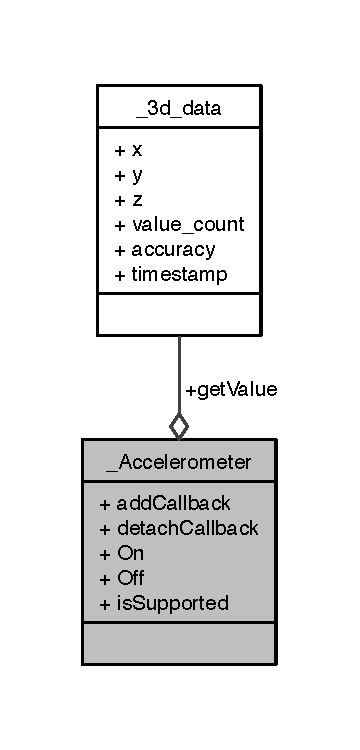
\includegraphics[width=173pt]{d5/d5a/struct__Accelerometer__coll__graph}
\end{center}
\end{figure}
\subsection*{Data Fields}
\begin{DoxyCompactItemize}
\item 
\hypertarget{struct__Accelerometer_a49a22e79a1d2f43397c0f2dd7b4b38b3}{bool($\ast$ {\bfseries add\-Callback} )(\hyperlink{struct__Accelerometer}{Accelerometer} this\-\_\-gen, sensor\-\_\-callback sensor\-Callback, int timeinterval, void $\ast$data)}\label{struct__Accelerometer_a49a22e79a1d2f43397c0f2dd7b4b38b3}

\item 
\hypertarget{struct__Accelerometer_a78f284559bbc8500ca54fa069369d4c6}{bool($\ast$ {\bfseries detach\-Callback} )(\hyperlink{struct__Accelerometer}{Accelerometer} this\-\_\-gen)}\label{struct__Accelerometer_a78f284559bbc8500ca54fa069369d4c6}

\item 
\hypertarget{struct__Accelerometer_a17eaafbdf2b40f38b82ad1cbb6025540}{bool($\ast$ {\bfseries On} )(\hyperlink{struct__Accelerometer}{Accelerometer} this\-\_\-gen)}\label{struct__Accelerometer_a17eaafbdf2b40f38b82ad1cbb6025540}

\item 
\hypertarget{struct__Accelerometer_ae9e0090f67466b06e0f14f59b4830990}{bool($\ast$ {\bfseries Off} )(\hyperlink{struct__Accelerometer}{Accelerometer} this\-\_\-gen)}\label{struct__Accelerometer_ae9e0090f67466b06e0f14f59b4830990}

\item 
\hypertarget{struct__Accelerometer_a0c01b8a5a915f39afb4429cbe3ee6d2c}{bool($\ast$ {\bfseries is\-Supported} )(\hyperlink{struct__Accelerometer}{Accelerometer} this\-\_\-gen)}\label{struct__Accelerometer_a0c01b8a5a915f39afb4429cbe3ee6d2c}

\item 
\hypertarget{struct__Accelerometer_a8c75dfb5dbc8f9da5ea69ef2fb597185}{\hyperlink{Sensor_8h_df/d29/struct__3d__data}{Accelerometer\-\_\-data}($\ast$ {\bfseries get\-Value} )(\hyperlink{struct__Accelerometer}{Accelerometer} this\-\_\-gen)}\label{struct__Accelerometer_a8c75dfb5dbc8f9da5ea69ef2fb597185}

\end{DoxyCompactItemize}


\subsection{Detailed Description}
Accelerometer 모듈에 대한 구조체이다. Accelerometer 모듈은 Accelerometer Sensor를 다양한 방식으로 제어할 수 있다. 

\begin{DoxyNote}{Note}
Accelerometer 모듈에 대한 구조체이다. \par
 구조체를 사용하기 전에 \hyperlink{Sensor_8h_abcf9601a4eab47e714e89190dc79ad50}{New\-Accelerometer()} 함수를 사용해야 하며 사용이 끝났을 때 \hyperlink{Sensor_8h_a275aeca9a471074bf414e5e9b817c8c1}{Destroy\-Accelerometer()} 함수를 꼭 사용해야 한다. 
\end{DoxyNote}
\begin{DoxySeeAlso}{See Also}
\href{https://developer.tizen.org/dev-guide/2.3.0/org.tizen.native.mobile.apireference/group__CAPI__SYSTEM__SENSOR__MODULE.html}{\tt https\-://developer.\-tizen.\-org/dev-\/guide/2.\-3.\-0/org.\-tizen.\-native.\-mobile.\-apireference/group\-\_\-\-\_\-\-C\-A\-P\-I\-\_\-\-\_\-\-S\-Y\-S\-T\-E\-M\-\_\-\-\_\-\-S\-E\-N\-S\-O\-R\-\_\-\-\_\-\-M\-O\-D\-U\-L\-E.\-html} 
\end{DoxySeeAlso}


Definition at line 121 of file Sensor.\-h.



The documentation for this struct was generated from the following file\-:\begin{DoxyCompactItemize}
\item 
\hyperlink{Sensor_8h}{Sensor.\-h}\end{DoxyCompactItemize}

\section{Audio Struct Reference}
\label{struct__Audio}\index{Audio@{Audio}}


Audio 모듈에 대한 구조체이다. Audio 모듈은 다양한 방식으로 음악 파일을 제어 할 수 있다.  




{\ttfamily \#include $<$File.\-h$>$}



Collaboration diagram for Audio\-:\nopagebreak
\begin{figure}[H]
\begin{center}
\leavevmode
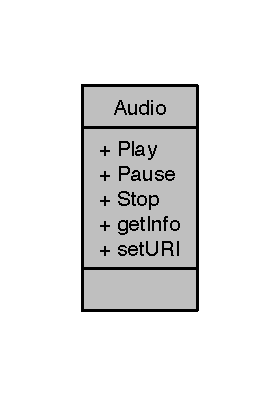
\includegraphics[width=134pt]{struct__Audio__coll__graph}
\end{center}
\end{figure}
\subsection*{Data Fields}
\begin{DoxyCompactItemize}
\item 
bool($\ast$ {\bfseries Play} )(Audio this\-\_\-gen)\label{struct__Audio_a2533056bdf8c73f787288908969451b6}

\item 
bool($\ast$ {\bfseries Pause} )(Audio this\-\_\-gen)\label{struct__Audio_a3f1043412c68fde6976ad12c4e04b562}

\item 
bool($\ast$ {\bfseries Stop} )(Audio this\-\_\-gen)\label{struct__Audio_a656614b835148875d471eb83d6c92d92}

\item 
String($\ast$ {\bfseries get\-Info} )(Audio this\-\_\-gen, metadata\-\_\-extractor\-\_\-attr\-\_\-e metadata\-Key)\label{struct__Audio_ace021bdc3095855893529b4a41e9668f}

\item 
bool($\ast$ {\bfseries set\-U\-R\-I} )(Audio this\-\_\-gen, String uri)\label{struct__Audio_a88de7890a374c4fe254bca82bd996395}

\end{DoxyCompactItemize}


\subsection{Detailed Description}
Audio 모듈에 대한 구조체이다. Audio 모듈은 다양한 방식으로 음악 파일을 제어 할 수 있다. 

\begin{DoxyNote}{Note}
File의 Audio 모듈에 대한 구조체이다. \par
 구조체를 사용하기 전에 \doxyref{New\-Audio()}{p.}{File_8h_abe7f8cf85bbeefba4700f61bc5877322} 함수를 사용해야 하며 사용이 끝났을 때 \doxyref{Destroy\-Audio()}{p.}{File_8h_a1c24d11e9397892d289591033dd8d174} 함수를 꼭 사용해야 한다. 
\end{DoxyNote}
\begin{DoxySeeAlso}{See Also}
{\tt Tizen Native A\-P\-I Document -\/ Audio part} 
\end{DoxySeeAlso}
\begin{DoxyPrecond}{Precondition}
{\bfseries privilege} \par

\begin{DoxyItemize}
\item {\tt http\-://tizen.\-org/privilege/mediastorage} \par

\item {\tt http\-://tizen.\-org/privilege/externalstorage} \par

\item {\tt http\-://tizen.\-org/privilege/internet} 
\end{DoxyItemize}
\end{DoxyPrecond}


The documentation for this struct was generated from the following file\-:\begin{DoxyCompactItemize}
\item 
{\bf File.\-h}\end{DoxyCompactItemize}

\section{Audio\-Recorder Struct Reference}
\label{struct__AudioRecorder}\index{Audio\-Recorder@{Audio\-Recorder}}


Audio\-Recorder 모듈에 대한 구조체이다. Audio\-Recorder 모듈은 음원을 녹음할 수 있다.  




{\ttfamily \#include $<$Media\-Recorder.\-h$>$}



Collaboration diagram for Audio\-Recorder\-:\nopagebreak
\begin{figure}[H]
\begin{center}
\leavevmode
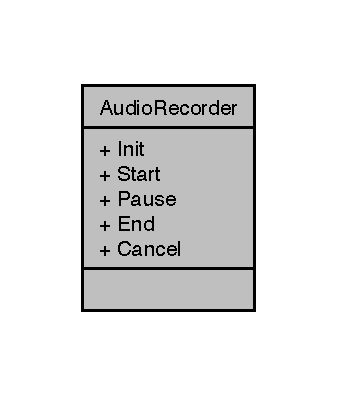
\includegraphics[width=162pt]{struct__AudioRecorder__coll__graph}
\end{center}
\end{figure}
\subsection*{Data Fields}
\begin{DoxyCompactItemize}
\item 
bool($\ast$ {\bfseries Init} )(Audio\-Recorder this\-\_\-gen, const String filename)\label{struct__AudioRecorder_aeac8a703c71a8d725a801a202ce15866}

\item 
bool($\ast$ {\bfseries Start} )(Audio\-Recorder this\-\_\-gen)\label{struct__AudioRecorder_a7b0b84a744f8f11e2c128599cf22076e}

\item 
bool($\ast$ {\bfseries Pause} )(Audio\-Recorder this\-\_\-gen)\label{struct__AudioRecorder_a135f2f30efe2b658c89959426768abdc}

\item 
bool($\ast$ {\bfseries End} )(Audio\-Recorder this\-\_\-gen)\label{struct__AudioRecorder_a647e10f47215e13990cb853f40ba3c9d}

\item 
bool($\ast$ {\bfseries Cancel} )(Audio\-Recorder this\-\_\-gen)\label{struct__AudioRecorder_a2a1482c37d01197a70e5f72aa114884d}

\end{DoxyCompactItemize}


\subsection{Detailed Description}
Audio\-Recorder 모듈에 대한 구조체이다. Audio\-Recorder 모듈은 음원을 녹음할 수 있다. 

\begin{DoxyNote}{Note}
Media Recorder의 Audio\-Recorder 모듈에 대한 구조체이다. \par
 구조체를 사용하기 전에 \doxyref{New\-Audio\-Recorder()}{p.}{MediaRecorder_8h_af96b985470296cf59ff534f9035dad36} 함수를 사용해야 하며 사용이 끝났을 때 \doxyref{Destroy\-Audio\-Recorder()}{p.}{MediaRecorder_8h_a97f3afce2235e4208952b52f9087c598} 함수를 꼭 사용해야 한다. 
\end{DoxyNote}
\begin{DoxySeeAlso}{See Also}
{\tt Tizen Native A\-P\-I Document -\/ Recorder part} 
\end{DoxySeeAlso}
\begin{DoxyPrecond}{Precondition}
{\bfseries privilege} \par

\begin{DoxyItemize}
\item {\tt http\-://tizen.\-org/privilege/recorder} \par

\item {\tt http\-://tizen.\-org/privilege/mediastorage} \par

\item {\tt http\-://tizen.\-org/privilege/externalstorage} \par

\end{DoxyItemize}

{\bfseries feature} \par

\begin{DoxyItemize}
\item {\tt http\-://tizen.\-org/feature/microphone} 
\end{DoxyItemize}
\end{DoxyPrecond}


The documentation for this struct was generated from the following file\-:\begin{DoxyCompactItemize}
\item 
{\bf Media\-Recorder.\-h}\end{DoxyCompactItemize}

\hypertarget{struct__Battery}{\section{\-\_\-\-Battery Struct Reference}
\label{struct__Battery}\index{\-\_\-\-Battery@{\-\_\-\-Battery}}
}


Battery 모듈에 대한 구조체이다. Battery 모듈은 배터리의 정보를 읽어 올 수 있다.  




{\ttfamily \#include $<$Device\-Status.\-h$>$}



Collaboration diagram for \-\_\-\-Battery\-:\nopagebreak
\begin{figure}[H]
\begin{center}
\leavevmode
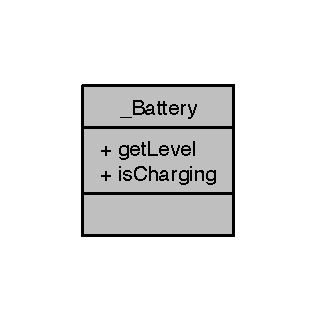
\includegraphics[width=152pt]{d3/d5f/struct__Battery__coll__graph}
\end{center}
\end{figure}
\subsection*{Data Fields}
\begin{DoxyCompactItemize}
\item 
\hypertarget{struct__Battery_a6321988705fe01fbbd13ed44645920ce}{int($\ast$ {\bfseries get\-Level} )(\hyperlink{struct__Battery}{Battery} this\-\_\-gen)}\label{struct__Battery_a6321988705fe01fbbd13ed44645920ce}

\item 
\hypertarget{struct__Battery_a58bd0a8a8a168cad5a323b2cef48f161}{bool($\ast$ {\bfseries is\-Charging} )(\hyperlink{struct__Battery}{Battery} this\-\_\-gen)}\label{struct__Battery_a58bd0a8a8a168cad5a323b2cef48f161}

\end{DoxyCompactItemize}


\subsection{Detailed Description}
Battery 모듈에 대한 구조체이다. Battery 모듈은 배터리의 정보를 읽어 올 수 있다. 

\begin{DoxyNote}{Note}
Device Status의 Battery 모듈에 대한 구조체이다. \par
 구조체를 사용하기 전에 \hyperlink{DeviceStatus_8h_a0fe7ab1f89e01e459f94bdecce693301}{New\-Battery()} 함수를 사용해야 하며 사용이 끝났을 때 \hyperlink{DeviceStatus_8h_a01b69d107b6708af6900d4279eeff281}{Destory\-Battery()} 함수를 꼭 사용해야 한다. 
\end{DoxyNote}
\begin{DoxySeeAlso}{See Also}
\href{https://developer.tizen.org/dev-guide/2.3.0/org.tizen.native.mobile.apireference/group__CAPI__SYSTEM__DEVICE__BATTERY__MODULE.html}{\tt https\-://developer.\-tizen.\-org/dev-\/guide/2.\-3.\-0/org.\-tizen.\-native.\-mobile.\-apireference/group\-\_\-\-\_\-\-C\-A\-P\-I\-\_\-\-\_\-\-S\-Y\-S\-T\-E\-M\-\_\-\-\_\-\-D\-E\-V\-I\-C\-E\-\_\-\-\_\-\-B\-A\-T\-T\-E\-R\-Y\-\_\-\-\_\-\-M\-O\-D\-U\-L\-E.\-html} 
\end{DoxySeeAlso}


Definition at line 322 of file Device\-Status.\-h.



The documentation for this struct was generated from the following file\-:\begin{DoxyCompactItemize}
\item 
\hyperlink{DeviceStatus_8h}{Device\-Status.\-h}\end{DoxyCompactItemize}

\hypertarget{struct__Bluetooth}{\section{\-\_\-\-Bluetooth Struct Reference}
\label{struct__Bluetooth}\index{\-\_\-\-Bluetooth@{\-\_\-\-Bluetooth}}
}


Bluetooth 모듈에 대한 구조체이다. Bluetooth 모듈은 다양한 방식으로 Bluetooth 통신을 할 수 있다.  




{\ttfamily \#include $<$Bluetooth.\-h$>$}



Collaboration diagram for \-\_\-\-Bluetooth\-:\nopagebreak
\begin{figure}[H]
\begin{center}
\leavevmode
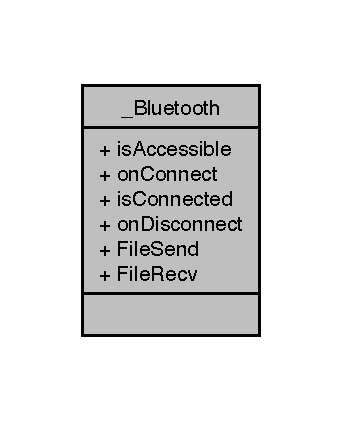
\includegraphics[width=164pt]{df/de6/struct__Bluetooth__coll__graph}
\end{center}
\end{figure}
\subsection*{Data Fields}
\begin{DoxyCompactItemize}
\item 
\hypertarget{struct__Bluetooth_a4d17357ef3f36198ec75747159ba463e}{bool($\ast$ {\bfseries is\-Accessible} )(\hyperlink{struct__Bluetooth}{Bluetooth} this\-\_\-gen)}\label{struct__Bluetooth_a4d17357ef3f36198ec75747159ba463e}

\item 
\hypertarget{struct__Bluetooth_a02ed8ce853ef7914c2d0663ddc85bf71}{bool($\ast$ {\bfseries on\-Connect} )(\hyperlink{struct__Bluetooth}{Bluetooth} this\-\_\-gen)}\label{struct__Bluetooth_a02ed8ce853ef7914c2d0663ddc85bf71}

\item 
\hypertarget{struct__Bluetooth_afaf7348f13265482f31f6bb326de23d3}{bool($\ast$ {\bfseries is\-Connected} )(\hyperlink{struct__Bluetooth}{Bluetooth} this\-\_\-gen)}\label{struct__Bluetooth_afaf7348f13265482f31f6bb326de23d3}

\item 
\hypertarget{struct__Bluetooth_a73fc8eb303afc5b6d5e9188e623f8d3d}{bool($\ast$ {\bfseries on\-Disconnect} )(\hyperlink{struct__Bluetooth}{Bluetooth} this\-\_\-gen)}\label{struct__Bluetooth_a73fc8eb303afc5b6d5e9188e623f8d3d}

\item 
\hypertarget{struct__Bluetooth_a32031c7a682e3eb8ccce66942ae01104}{bool($\ast$ {\bfseries File\-Send} )(\hyperlink{struct__Bluetooth}{Bluetooth} this\-\_\-gen, String send\-Buffer)}\label{struct__Bluetooth_a32031c7a682e3eb8ccce66942ae01104}

\item 
\hypertarget{struct__Bluetooth_ab7586458920997808d8564b5d337a60b}{bool($\ast$ {\bfseries File\-Recv} )(\hyperlink{struct__Bluetooth}{Bluetooth} this\-\_\-gen, String $\ast$recv\-Buffer)}\label{struct__Bluetooth_ab7586458920997808d8564b5d337a60b}

\end{DoxyCompactItemize}


\subsection{Detailed Description}
Bluetooth 모듈에 대한 구조체이다. Bluetooth 모듈은 다양한 방식으로 Bluetooth 통신을 할 수 있다. 

\begin{DoxyNote}{Note}
Bluetooth의 Bluetooth 모듈에 대한 구조체이다. \par
 구조체를 사용하기 전에 \hyperlink{Bluetooth_8h_aedecb2f1b25b6d408a1880978b66712a}{New\-Bluetooth()} 함수를 사용해야 하며 사용이 끝났을 때 \hyperlink{Bluetooth_8h_a643b6a392ddbcf1c02bcfeb15ca52df8}{Destroy\-Bluetooth()} 함수를 꼭 사용해야 한다. 
\end{DoxyNote}
\begin{DoxySeeAlso}{See Also}
\href{https://developer.tizen.org/dev-guide/2.3.0/org.tizen.native.mobile.apireference/group__CAPI__NETWORK__BLUETOOTH__MODULE.html}{\tt Tizen Native A\-P\-I Document -\/ Bluetooth part} 
\end{DoxySeeAlso}
\begin{DoxyPrecond}{Precondition}
{\bfseries feature} \par

\begin{DoxyItemize}
\item \href{http://tizen.org/feature/network.bluetooth}{\tt http\-://tizen.\-org/feature/network.\-bluetooth} \par

\item ddddddddddddddddd \par
 {\bfseries priviledge} \par

\item \href{http://tizen.org/feature/network.bluetooth}{\tt http\-://tizen.\-org/feature/network.\-bluetooth} \par

\end{DoxyItemize}
\end{DoxyPrecond}


Definition at line 70 of file Bluetooth.\-h.



The documentation for this struct was generated from the following file\-:\begin{DoxyCompactItemize}
\item 
\hyperlink{Bluetooth_8h}{Bluetooth.\-h}\end{DoxyCompactItemize}

\section{Camera\-Recorder Struct Reference}
\label{struct__CameraRecorder}\index{Camera\-Recorder@{Camera\-Recorder}}


Camera\-Recorder 모듈에 대한 구조체이다. Camera\-Recorder 모듈은 동영상을 녹화할 수 있다.  




{\ttfamily \#include $<$Media\-Recorder.\-h$>$}



Collaboration diagram for Camera\-Recorder\-:
\nopagebreak
\begin{figure}[H]
\begin{center}
\leavevmode
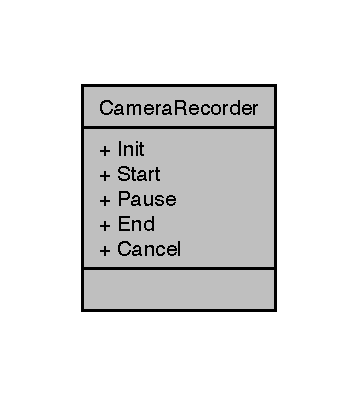
\includegraphics[width=172pt]{struct__CameraRecorder__coll__graph}
\end{center}
\end{figure}
\subsection*{Data Fields}
\begin{DoxyCompactItemize}
\item 
bool($\ast$ {\bfseries Init} )(Camera\-Recorder this\-\_\-gen, const String filename, camera\-\_\-type camera, Evas\-\_\-\-Object $\ast$evas\-Object)\label{struct__CameraRecorder_a96d7c4905492495101ed5438530c2543}

\item 
bool($\ast$ {\bfseries Start} )(Camera\-Recorder this\-\_\-gen)\label{struct__CameraRecorder_aa5d3fc3bf8c7fafac1cdb2f531fe8d24}

\item 
bool($\ast$ {\bfseries Pause} )(Camera\-Recorder this\-\_\-gen)\label{struct__CameraRecorder_a6ca0baf56971d59353e4c9ee48848b02}

\item 
bool($\ast$ {\bfseries End} )(Camera\-Recorder this\-\_\-gen)\label{struct__CameraRecorder_a5529a506cfd2c835306085d0fa8e6d3c}

\item 
bool($\ast$ {\bfseries Cancel} )(Camera\-Recorder this\-\_\-gen)\label{struct__CameraRecorder_adc473d693f9aa9c57ecdd7aeacf110b2}

\end{DoxyCompactItemize}


\subsection{Detailed Description}
Camera\-Recorder 모듈에 대한 구조체이다. Camera\-Recorder 모듈은 동영상을 녹화할 수 있다. 

\begin{DoxyNote}{Note}
Media Recorder의 Camera\-Recorder 모듈에 대한 구조체이다. \par
 구조체를 사용하기 전에 \doxyref{New\-Camera\-Recorder()}{p.}{MediaRecorder_8h_a7bbb16d9e9a7aa0d54f9a576573154b5} 함수를 사용해야 하며 사용이 끝났을 때 \doxyref{Destroy\-Audio\-Recorder()}{p.}{MediaRecorder_8h_a97f3afce2235e4208952b52f9087c598} 함수를 꼭 사용해야 한다. 
\end{DoxyNote}
\begin{DoxySeeAlso}{See Also}
{\tt Tizen Native A\-P\-I Document -\/ Recorder part} 
\end{DoxySeeAlso}
\begin{DoxyPrecond}{Precondition}
{\bfseries privilege} \par

\begin{DoxyItemize}
\item {\tt http\-://tizen.\-org/privilege/recorder} \par

\item {\tt http\-://tizen.\-org/privilege/mediastorage} \par

\item {\tt http\-://tizen.\-org/privilege/externalstorage} \par

\end{DoxyItemize}

{\bfseries feature} \par

\begin{DoxyItemize}
\item {\tt http\-://tizen.\-org/feature/camera} \par

\item {\tt http\-://tizen.\-org/feature/microphone} 
\end{DoxyItemize}
\end{DoxyPrecond}


The documentation for this struct was generated from the following file\-:\begin{DoxyCompactItemize}
\item 
{\bf Media\-Recorder.\-h}\end{DoxyCompactItemize}

\section{Display Struct Reference}
\label{struct__Display}\index{Display@{Display}}


Display 모듈에 대한 구조체이다. Display 모듈은 다양한 방식으로 화면을 조절 할 수 있다.  




{\ttfamily \#include $<$Device\-Status.\-h$>$}



Collaboration diagram for Display\-:\nopagebreak
\begin{figure}[H]
\begin{center}
\leavevmode
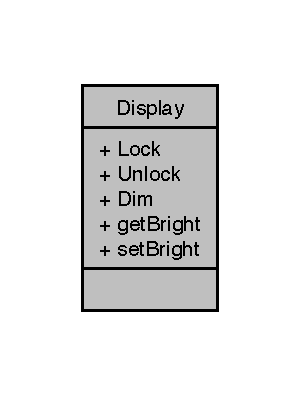
\includegraphics[width=144pt]{struct__Display__coll__graph}
\end{center}
\end{figure}
\subsection*{Data Fields}
\begin{DoxyCompactItemize}
\item 
bool($\ast$ {\bfseries Lock} )(Display this\-\_\-gen)\label{struct__Display_ae63a3abcf51257dbc7f94817504953e9}

\item 
bool($\ast$ {\bfseries Unlock} )(Display this\-\_\-gen)\label{struct__Display_a30c16960b10431b893543a04a25d282f}

\item 
bool($\ast$ {\bfseries Dim} )(Display this\-\_\-gen)\label{struct__Display_a244281b52b37bea0fc4ecc449e94892b}

\item 
int($\ast$ {\bfseries get\-Bright} )(Display this\-\_\-gen)\label{struct__Display_a4496ff482b37623f947cb8104f0d1bc3}

\item 
bool($\ast$ {\bfseries set\-Bright} )(Display this\-\_\-gen, int bright)\label{struct__Display_a8fa8f7fa9933f014e0ca2ededdc3a648}

\end{DoxyCompactItemize}


\subsection{Detailed Description}
Display 모듈에 대한 구조체이다. Display 모듈은 다양한 방식으로 화면을 조절 할 수 있다. 

\begin{DoxyNote}{Note}
Device Status의 Display 모듈에 대한 구조체이다. \par
 구조체를 사용하기 전에 \doxyref{New\-Display()}{p.}{DeviceStatus_8h_a239d9485c4000ae77b11e5f12378f95f} 함수를 사용해야 하며 사용이 끝났을 때 \doxyref{Destroy\-Display()}{p.}{DeviceStatus_8h_aa18ddc0342d1ca47145c759a8fa35d91} 함수를 꼭 사용해야 한다. 
\end{DoxyNote}
\begin{DoxySeeAlso}{See Also}
{\tt Tizen Native A\-P\-I Document -\/ Display part} 
\end{DoxySeeAlso}
\begin{DoxyPrecond}{Precondition}
{\bfseries privilege} \par

\begin{DoxyItemize}
\item {\tt http\-://tizen.\-org/privilege/display} 
\end{DoxyItemize}
\end{DoxyPrecond}


The documentation for this struct was generated from the following file\-:\begin{DoxyCompactItemize}
\item 
{\bf Device\-Status.\-h}\end{DoxyCompactItemize}

\section{File Struct Reference}
\label{struct__File}\index{File@{File}}


File 모듈에 대한 구조체이다. File 모듈은 다양한 방식으로 파일을 제어 할 수 있다.  




{\ttfamily \#include $<$File.\-h$>$}



Collaboration diagram for File\-:
\nopagebreak
\begin{figure}[H]
\begin{center}
\leavevmode
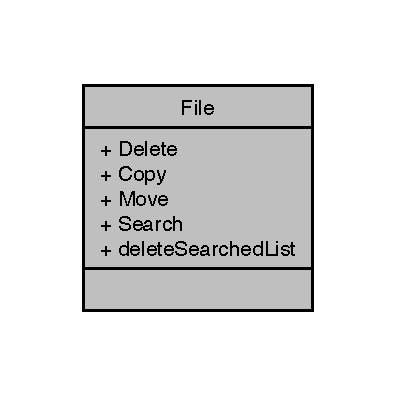
\includegraphics[width=190pt]{struct__File__coll__graph}
\end{center}
\end{figure}
\subsection*{Data Fields}
\begin{DoxyCompactItemize}
\item 
bool($\ast$ {\bfseries Delete} )(String src)\label{struct__File_adf274a397a0985b8a8675c15efc8829a}

\item 
bool($\ast$ {\bfseries Copy} )(String src, String dst)\label{struct__File_a2f79e552b30735dabf7cc0e7f0b88b6c}

\item 
bool($\ast$ {\bfseries Move} )(String src, String dst)\label{struct__File_a1a27af6781f09718e0f9b9802ef3d9e5}

\item 
G\-List $\ast$($\ast$ {\bfseries Search} )(String src, String dst)\label{struct__File_a53ec46e614def6722aa115461f377ec1}

\item 
void($\ast$ {\bfseries delete\-Searched\-List} )(G\-List $\ast$searched\-List)\label{struct__File_a99be93124b91f4c2c66704e6b49dc6ef}

\end{DoxyCompactItemize}


\subsection{Detailed Description}
File 모듈에 대한 구조체이다. File 모듈은 다양한 방식으로 파일을 제어 할 수 있다. 

\begin{DoxyNote}{Note}
File의 File 모듈에 대한 구조체이다. \par
 구조체를 사용하기 전에 \doxyref{New\-File()}{p.}{File_8h_a9dc7e152baf123500677519b3d311532} 함수를 사용해야 하며 사용이 끝났을 때 \doxyref{Destroy\-File()}{p.}{File_8h_ab44ac1360d2598918dd2c655833e10c0} 함수를 꼭 사용해야 한다. 
\end{DoxyNote}
\begin{DoxySeeAlso}{See Also}
{\tt Tizen Native A\-P\-I Document -\/ File part} 
\end{DoxySeeAlso}
\begin{DoxyPrecond}{Precondition}
{\bfseries privilege} \par

\begin{DoxyItemize}
\item {\tt http\-://tizen.\-org/privilege/mediastorage} \par

\item {\tt http\-://tizen.\-org/privilege/externalstorage} 
\end{DoxyItemize}
\end{DoxyPrecond}


The documentation for this struct was generated from the following file\-:\begin{DoxyCompactItemize}
\item 
{\bf File.\-h}\end{DoxyCompactItemize}

\hypertarget{struct__Flash}{\section{\-\_\-\-Flash Struct Reference}
\label{struct__Flash}\index{\-\_\-\-Flash@{\-\_\-\-Flash}}
}


Flash 모듈에 대한 구조체이다. Flash 모듈은 Device의 플래시를 제어 할 수 있다.  




{\ttfamily \#include $<$Device\-Status.\-h$>$}



Collaboration diagram for \-\_\-\-Flash\-:\nopagebreak
\begin{figure}[H]
\begin{center}
\leavevmode
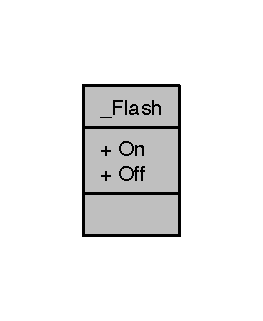
\includegraphics[width=126pt]{da/d34/struct__Flash__coll__graph}
\end{center}
\end{figure}
\subsection*{Data Fields}
\begin{DoxyCompactItemize}
\item 
\hypertarget{struct__Flash_ae123319afef15c36b1d52f41184e2387}{bool($\ast$ {\bfseries On} )(void)}\label{struct__Flash_ae123319afef15c36b1d52f41184e2387}

\item 
\hypertarget{struct__Flash_a9cba109cd9391d9c09b3a7b46a345dad}{bool($\ast$ {\bfseries Off} )(void)}\label{struct__Flash_a9cba109cd9391d9c09b3a7b46a345dad}

\end{DoxyCompactItemize}


\subsection{Detailed Description}
Flash 모듈에 대한 구조체이다. Flash 모듈은 Device의 플래시를 제어 할 수 있다. 

\begin{DoxyNote}{Note}
Device Status의 Flash 모듈에 대한 구조체이다. \par
 구조체를 사용하기 전에 \hyperlink{DeviceStatus_8h_a503e0814548cc9f370f87a3359187bff}{New\-Flash()} 함수를 사용해야 하며 사용이 끝났을 때 \hyperlink{DeviceStatus_8h_a4d0567730f41384d32902ef2b7c4b242}{Destory\-Flash()} 함수를 꼭 사용해야 한다. 
\end{DoxyNote}
\begin{DoxySeeAlso}{See Also}
\href{https://developer.tizen.org/dev-guide/2.3.0/org.tizen.native.mobile.apireference/group__CAPI__SYSTEM__DEVICE__LED__MODULE.html}{\tt https\-://developer.\-tizen.\-org/dev-\/guide/2.\-3.\-0/org.\-tizen.\-native.\-mobile.\-apireference/group\-\_\-\-\_\-\-C\-A\-P\-I\-\_\-\-\_\-\-S\-Y\-S\-T\-E\-M\-\_\-\-\_\-\-D\-E\-V\-I\-C\-E\-\_\-\-\_\-\-L\-E\-D\-\_\-\-\_\-\-M\-O\-D\-U\-L\-E.\-html} 
\end{DoxySeeAlso}
\begin{DoxyPrecond}{Precondition}
privilege에 \char`\"{}http\-://tizen.\-org/privilege/led\char`\"{} 를 반드시 추가해야 한다. \par
 features에 \char`\"{}http\-://tizen.\-org/feature/led\char`\"{} 를 반드시 추가한다. \par
 features에 \char`\"{}http\-://tizen.\-org/feature/camera.\-back.\-flash\char`\"{} 를 반드시 추가한다. 
\end{DoxyPrecond}


Definition at line 397 of file Device\-Status.\-h.



The documentation for this struct was generated from the following file\-:\begin{DoxyCompactItemize}
\item 
\hyperlink{DeviceStatus_8h}{Device\-Status.\-h}\end{DoxyCompactItemize}

\hypertarget{struct__gps}{\section{\-\_\-gps 구조체 참조}
\label{struct__gps}\index{\-\_\-gps@{\-\_\-gps}}
}


{\ttfamily \#include $<$G\-P\-S.\-h$>$}

\subsection*{데이타 필드}
\begin{DoxyCompactItemize}
\item 
bool($\ast$ \hyperlink{struct__gps_ab422e6e9531279ce2cf7836d6fdad824}{is\-Accessible} )(\hyperlink{_g_p_s_8h_abd7b5738587f7a619dbeddcd69e8a319}{G\-P\-S} this\-\_\-gen)
\item 
bool($\ast$ \hyperlink{struct__gps_ac1e7688363e326df6919afc5d8cc848c}{on\-Connect} )(\hyperlink{_g_p_s_8h_abd7b5738587f7a619dbeddcd69e8a319}{G\-P\-S} this\-\_\-gen)
\item 
bool($\ast$ \hyperlink{struct__gps_a7ad2cd5581984147767aa12d71a7ff74}{on\-Disconnect} )(\hyperlink{_g_p_s_8h_abd7b5738587f7a619dbeddcd69e8a319}{G\-P\-S} this\-\_\-gen)
\item 
\hyperlink{_g_p_s_8h_ac4745ca529cacca07c33d7d83cce62c9}{Location}($\ast$ \hyperlink{struct__gps_a983b023f987a119a6df5c57b8a998f61}{Recv} )(\hyperlink{_g_p_s_8h_abd7b5738587f7a619dbeddcd69e8a319}{G\-P\-S} this\-\_\-gen)
\end{DoxyCompactItemize}


\subsection{상세한 설명}


G\-P\-S.\-h 파일의 29 번째 라인에서 정의되었습니다.



\subsection{필드 문서화}
\hypertarget{struct__gps_ab422e6e9531279ce2cf7836d6fdad824}{\index{\-\_\-gps@{\-\_\-gps}!is\-Accessible@{is\-Accessible}}
\index{is\-Accessible@{is\-Accessible}!_gps@{\-\_\-gps}}
\subsubsection[{is\-Accessible}]{\setlength{\rightskip}{0pt plus 5cm}bool($\ast$  is\-Accessible)({\bf G\-P\-S} this\-\_\-gen)}}\label{struct__gps_ab422e6e9531279ce2cf7836d6fdad824}


G\-P\-S.\-h 파일의 31 번째 라인에서 정의되었습니다.

\hypertarget{struct__gps_ac1e7688363e326df6919afc5d8cc848c}{\index{\-\_\-gps@{\-\_\-gps}!on\-Connect@{on\-Connect}}
\index{on\-Connect@{on\-Connect}!_gps@{\-\_\-gps}}
\subsubsection[{on\-Connect}]{\setlength{\rightskip}{0pt plus 5cm}bool($\ast$  on\-Connect)({\bf G\-P\-S} this\-\_\-gen)}}\label{struct__gps_ac1e7688363e326df6919afc5d8cc848c}


G\-P\-S.\-h 파일의 33 번째 라인에서 정의되었습니다.

\hypertarget{struct__gps_a7ad2cd5581984147767aa12d71a7ff74}{\index{\-\_\-gps@{\-\_\-gps}!on\-Disconnect@{on\-Disconnect}}
\index{on\-Disconnect@{on\-Disconnect}!_gps@{\-\_\-gps}}
\subsubsection[{on\-Disconnect}]{\setlength{\rightskip}{0pt plus 5cm}bool($\ast$  on\-Disconnect)({\bf G\-P\-S} this\-\_\-gen)}}\label{struct__gps_a7ad2cd5581984147767aa12d71a7ff74}


G\-P\-S.\-h 파일의 35 번째 라인에서 정의되었습니다.

\hypertarget{struct__gps_a983b023f987a119a6df5c57b8a998f61}{\index{\-\_\-gps@{\-\_\-gps}!Recv@{Recv}}
\index{Recv@{Recv}!_gps@{\-\_\-gps}}
\subsubsection[{Recv}]{\setlength{\rightskip}{0pt plus 5cm}{\bf Location}($\ast$  Recv)({\bf G\-P\-S} this\-\_\-gen)}}\label{struct__gps_a983b023f987a119a6df5c57b8a998f61}


G\-P\-S.\-h 파일의 37 번째 라인에서 정의되었습니다.



이 구조체에 대한 문서화 페이지는 다음의 파일로부터 생성되었습니다.\-:\begin{DoxyCompactItemize}
\item 
\hyperlink{_g_p_s_8h}{G\-P\-S.\-h}\end{DoxyCompactItemize}

\section{Gravity Struct Reference}
\label{struct__Gravity}\index{Gravity@{Gravity}}


Gravity 모듈에 대한 구조체이다. Gravity 모듈은 Gravity Sensor를 다양한 방식으로 제어할 수 있다.  




{\ttfamily \#include $<$Sensor.\-h$>$}



Collaboration diagram for Gravity\-:\nopagebreak
\begin{figure}[H]
\begin{center}
\leavevmode
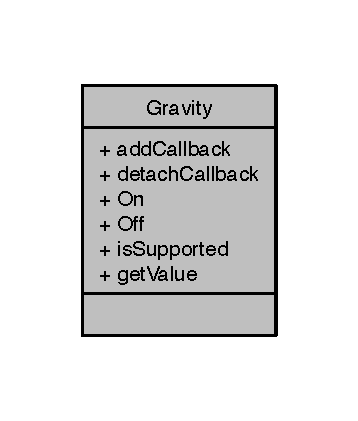
\includegraphics[width=172pt]{struct__Gravity__coll__graph}
\end{center}
\end{figure}
\subsection*{Data Fields}
\begin{DoxyCompactItemize}
\item 
bool($\ast$ {\bfseries add\-Callback} )(Gravity this\-\_\-gen, sensor\-\_\-callback sensor\-Callback, int timeinterval, void $\ast$data)\label{struct__Gravity_a138736bfc3d4fff133c938b173031b02}

\item 
bool($\ast$ {\bfseries detach\-Callback} )(Gravity this\-\_\-gen)\label{struct__Gravity_a99ff1e248087163600fd61db54f91cb2}

\item 
bool($\ast$ {\bfseries On} )(Gravity this\-\_\-gen)\label{struct__Gravity_ad36fdb2df66c142cc6ed7b97ca6fff87}

\item 
bool($\ast$ {\bfseries Off} )(Gravity this\-\_\-gen)\label{struct__Gravity_a8515dc119b3228a1feffd287134eef7e}

\item 
bool($\ast$ {\bfseries is\-Supported} )(Gravity this\-\_\-gen)\label{struct__Gravity_a500b049aa54b528ae9ee1a68e49f3b22}

\item 
Gravity\-\_\-data($\ast$ {\bfseries get\-Value} )(Gravity this\-\_\-gen)\label{struct__Gravity_a1fb6f67d7ba292e2a5247862d34aeca6}

\end{DoxyCompactItemize}


\subsection{Detailed Description}
Gravity 모듈에 대한 구조체이다. Gravity 모듈은 Gravity Sensor를 다양한 방식으로 제어할 수 있다. 

\begin{DoxyNote}{Note}
Gravity 모듈에 대한 구조체이다. \par
 구조체를 사용하기 전에 \doxyref{New\-Gravity()}{p.}{Sensor_8h_a300e5404c843b1366edef9183be709c6} 함수를 사용해야 하며 사용이 끝났을 때 \doxyref{Destroy\-Gravity()}{p.}{Sensor_8h_a4ac22619e930846038a60e69536844db} 함수를 꼭 사용해야 한다. 
\end{DoxyNote}
\begin{DoxySeeAlso}{See Also}
{\tt Tizen Native A\-P\-I Document -\/ Sensor part} 
\end{DoxySeeAlso}
\begin{DoxyPrecond}{Precondition}
{\bfseries feature} \par

\begin{DoxyItemize}
\item {\tt http\-://tizen.\-org/feature/sensor.\-gravity} 
\end{DoxyItemize}
\end{DoxyPrecond}


The documentation for this struct was generated from the following file\-:\begin{DoxyCompactItemize}
\item 
{\bf Sensor.\-h}\end{DoxyCompactItemize}

\hypertarget{struct__Gyroscope}{\section{\-\_\-\-Gyroscope Struct Reference}
\label{struct__Gyroscope}\index{\-\_\-\-Gyroscope@{\-\_\-\-Gyroscope}}
}


Gyroscope 모듈에 대한 구조체이다. Gyroscope 모듈은 Gyroscope Sensor를 다양한 방식으로 제어할 수 있다.  




{\ttfamily \#include $<$Sensor.\-h$>$}



Collaboration diagram for \-\_\-\-Gyroscope\-:\nopagebreak
\begin{figure}[H]
\begin{center}
\leavevmode
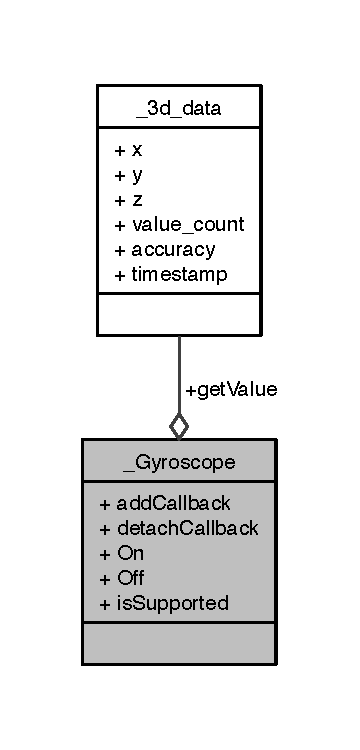
\includegraphics[width=173pt]{d8/d92/struct__Gyroscope__coll__graph}
\end{center}
\end{figure}
\subsection*{Data Fields}
\begin{DoxyCompactItemize}
\item 
\hypertarget{struct__Gyroscope_a8ed204dd4cf27c9ed2995c2f54a39dc3}{bool($\ast$ {\bfseries add\-Callback} )(\hyperlink{struct__Gyroscope}{Gyroscope} this\-\_\-gen, sensor\-\_\-callback sensor\-Callback, int timeinterval, void $\ast$data)}\label{struct__Gyroscope_a8ed204dd4cf27c9ed2995c2f54a39dc3}

\item 
\hypertarget{struct__Gyroscope_a8563723f9f86ef959ae1209f2fbf7645}{bool($\ast$ {\bfseries detach\-Callback} )(\hyperlink{struct__Gyroscope}{Gyroscope} this\-\_\-gen)}\label{struct__Gyroscope_a8563723f9f86ef959ae1209f2fbf7645}

\item 
\hypertarget{struct__Gyroscope_a65cf092766f15c09f9e052d4e9932869}{bool($\ast$ {\bfseries On} )(\hyperlink{struct__Gyroscope}{Gyroscope} this\-\_\-gen)}\label{struct__Gyroscope_a65cf092766f15c09f9e052d4e9932869}

\item 
\hypertarget{struct__Gyroscope_afe811258869c9f8b112ea029df3d1fae}{bool($\ast$ {\bfseries Off} )(\hyperlink{struct__Gyroscope}{Gyroscope} this\-\_\-gen)}\label{struct__Gyroscope_afe811258869c9f8b112ea029df3d1fae}

\item 
\hypertarget{struct__Gyroscope_ac0f373cd10a93722406c823688676dee}{bool($\ast$ {\bfseries is\-Supported} )(\hyperlink{struct__Gyroscope}{Gyroscope} this\-\_\-gen)}\label{struct__Gyroscope_ac0f373cd10a93722406c823688676dee}

\item 
\hypertarget{struct__Gyroscope_a9e5519a135ce1a2b58d7e21fd2d53171}{\hyperlink{Sensor_8h_df/d29/struct__3d__data}{Gyroscope\-\_\-data}($\ast$ {\bfseries get\-Value} )(\hyperlink{struct__Gyroscope}{Gyroscope} this\-\_\-gen)}\label{struct__Gyroscope_a9e5519a135ce1a2b58d7e21fd2d53171}

\end{DoxyCompactItemize}


\subsection{Detailed Description}
Gyroscope 모듈에 대한 구조체이다. Gyroscope 모듈은 Gyroscope Sensor를 다양한 방식으로 제어할 수 있다. 

\begin{DoxyNote}{Note}
Gyroscope 모듈에 대한 구조체이다. \par
 구조체를 사용하기 전에 \hyperlink{Sensor_8h_aad893caaae4e3153286926b76443bcf2}{New\-Gyroscope()} 함수를 사용해야 하며 사용이 끝났을 때 \hyperlink{Sensor_8h_a33c4827cef482ac97b726c6afd4f2c02}{Destroy\-Gyroscope()} 함수를 꼭 사용해야 한다. 
\end{DoxyNote}
\begin{DoxySeeAlso}{See Also}
\href{https://developer.tizen.org/dev-guide/2.3.0/org.tizen.native.mobile.apireference/group__CAPI__SYSTEM__SENSOR__MODULE.html}{\tt https\-://developer.\-tizen.\-org/dev-\/guide/2.\-3.\-0/org.\-tizen.\-native.\-mobile.\-apireference/group\-\_\-\-\_\-\-C\-A\-P\-I\-\_\-\-\_\-\-S\-Y\-S\-T\-E\-M\-\_\-\-\_\-\-S\-E\-N\-S\-O\-R\-\_\-\-\_\-\-M\-O\-D\-U\-L\-E.\-html} 
\end{DoxySeeAlso}


Definition at line 1178 of file Sensor.\-h.



The documentation for this struct was generated from the following file\-:\begin{DoxyCompactItemize}
\item 
\hyperlink{Sensor_8h}{Sensor.\-h}\end{DoxyCompactItemize}

\hypertarget{struct__Http}{\section{\-\_\-\-Http Struct Reference}
\label{struct__Http}\index{\-\_\-\-Http@{\-\_\-\-Http}}
}


Http 모듈에 대한 구조체이다. Http 모듈은 다양한 방식으로 Http 통신을 할 수 있다.  




{\ttfamily \#include $<$Http.\-h$>$}



Collaboration diagram for \-\_\-\-Http\-:\nopagebreak
\begin{figure}[H]
\begin{center}
\leavevmode
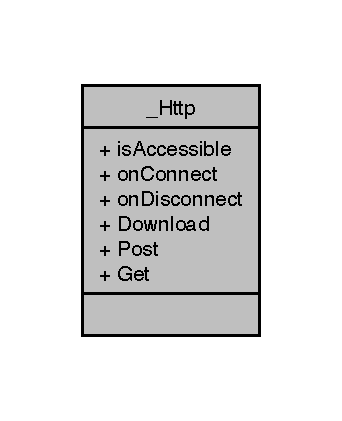
\includegraphics[width=164pt]{d8/d80/struct__Http__coll__graph}
\end{center}
\end{figure}
\subsection*{Data Fields}
\begin{DoxyCompactItemize}
\item 
\hypertarget{struct__Http_a3f21ba58588b0d2e11e7611caf3fa65c}{bool($\ast$ {\bfseries is\-Accessible} )(\hyperlink{struct__Http}{Http} this\-\_\-gen)}\label{struct__Http_a3f21ba58588b0d2e11e7611caf3fa65c}

\item 
\hypertarget{struct__Http_a952cc07a3505431bf33a7a6393a1503a}{bool($\ast$ {\bfseries on\-Connect} )(\hyperlink{struct__Http}{Http} this\-\_\-gen, String url, int port)}\label{struct__Http_a952cc07a3505431bf33a7a6393a1503a}

\item 
\hypertarget{struct__Http_ad6d1f6047ef195fe434e3d259aa0375a}{bool($\ast$ {\bfseries on\-Disconnect} )(\hyperlink{struct__Http}{Http} this\-\_\-gen)}\label{struct__Http_ad6d1f6047ef195fe434e3d259aa0375a}

\item 
\hypertarget{struct__Http_ab1e77582577b37757ed378ed3f86d298}{bool($\ast$ {\bfseries Download} )(\hyperlink{struct__Http}{Http} this\-\_\-gen, String filename)}\label{struct__Http_ab1e77582577b37757ed378ed3f86d298}

\item 
\hypertarget{struct__Http_af5fa9b3c938bda9972d5e4b9f880835b}{bool($\ast$ {\bfseries Post} )(\hyperlink{struct__Http}{Http} this\-\_\-gen, String res, String $\ast$req)}\label{struct__Http_af5fa9b3c938bda9972d5e4b9f880835b}

\item 
\hypertarget{struct__Http_ae18bf127b32304b57ce442c8282fe73a}{bool($\ast$ {\bfseries Get} )(\hyperlink{struct__Http}{Http} this\-\_\-gen, String res, String $\ast$req)}\label{struct__Http_ae18bf127b32304b57ce442c8282fe73a}

\end{DoxyCompactItemize}


\subsection{Detailed Description}
Http 모듈에 대한 구조체이다. Http 모듈은 다양한 방식으로 Http 통신을 할 수 있다. 

\begin{DoxyNote}{Note}
Http의 Http 모듈에 대한 구조체이다. \par
 구조체를 사용하기 전에 \hyperlink{Http_8h_a8f651c47670c3bb629ce2fe7e5d64d57}{New\-Http()} 함수를 사용해야 하며 사용이 끝났을 때 \hyperlink{Http_8h_afc5917bb56ffeda1df7514c8238f0cc4}{Destory\-Http()} 함수를 꼭 사용해야 한다. 
\end{DoxyNote}
\begin{DoxySeeAlso}{See Also}
\href{https://developer.tizen.org/dev-guide/2.3.0/org.tizen.native.mobile.apireference/group__OPENSRC__CURL__FRAMEWORK.html}{\tt https\-://developer.\-tizen.\-org/dev-\/guide/2.\-3.\-0/org.\-tizen.\-native.\-mobile.\-apireference/group\-\_\-\-\_\-\-O\-P\-E\-N\-S\-R\-C\-\_\-\-\_\-\-C\-U\-R\-L\-\_\-\-\_\-\-F\-R\-A\-M\-E\-W\-O\-R\-K.\-html} 
\end{DoxySeeAlso}
\begin{DoxyPrecond}{Precondition}
privilege에 \char`\"{}http\-://tizen.\-org/privilege/internet\char`\"{} 을 반드시 추가해야 한다. 
\end{DoxyPrecond}


Definition at line 120 of file Http.\-h.



The documentation for this struct was generated from the following file\-:\begin{DoxyCompactItemize}
\item 
\hyperlink{Http_8h}{Http.\-h}\end{DoxyCompactItemize}

\hypertarget{struct__Humidity}{\section{\-\_\-\-Humidity Struct Reference}
\label{struct__Humidity}\index{\-\_\-\-Humidity@{\-\_\-\-Humidity}}
}


Humidity 모듈에 대한 구조체이다. Humidity 모듈은 Humidity Sensor를 다양한 방식으로 제어할 수 있다.  




{\ttfamily \#include $<$Sensor.\-h$>$}



Collaboration diagram for \-\_\-\-Humidity\-:\nopagebreak
\begin{figure}[H]
\begin{center}
\leavevmode
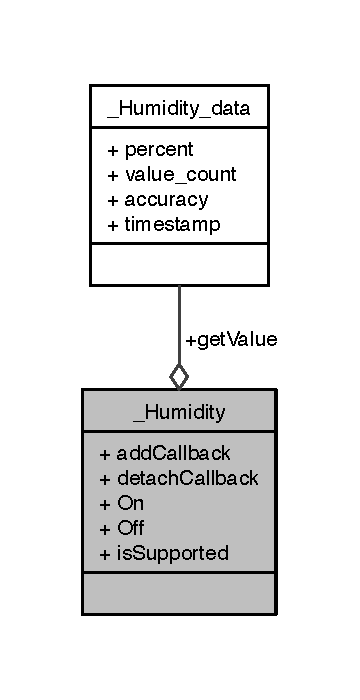
\includegraphics[width=173pt]{d5/d8c/struct__Humidity__coll__graph}
\end{center}
\end{figure}
\subsection*{Data Fields}
\begin{DoxyCompactItemize}
\item 
\hypertarget{struct__Humidity_ae020e34ba54ea361a9fabce5bc3e9467}{bool($\ast$ {\bfseries add\-Callback} )(\hyperlink{struct__Humidity}{Humidity} this\-\_\-gen, sensor\-\_\-callback sensor\-Callback, int timeinterval, void $\ast$data)}\label{struct__Humidity_ae020e34ba54ea361a9fabce5bc3e9467}

\item 
\hypertarget{struct__Humidity_ae00fb0f7d2a7a4c1f3a865019ddf157c}{bool($\ast$ {\bfseries detach\-Callback} )(\hyperlink{struct__Humidity}{Humidity} this\-\_\-gen)}\label{struct__Humidity_ae00fb0f7d2a7a4c1f3a865019ddf157c}

\item 
\hypertarget{struct__Humidity_a0feebb4da2daa33a6a2c44caafc985b4}{bool($\ast$ {\bfseries On} )(\hyperlink{struct__Humidity}{Humidity} this\-\_\-gen)}\label{struct__Humidity_a0feebb4da2daa33a6a2c44caafc985b4}

\item 
\hypertarget{struct__Humidity_a67ae0522e0566cf1ee22346f1e45a41b}{bool($\ast$ {\bfseries Off} )(\hyperlink{struct__Humidity}{Humidity} this\-\_\-gen)}\label{struct__Humidity_a67ae0522e0566cf1ee22346f1e45a41b}

\item 
\hypertarget{struct__Humidity_adda26eb4f1a4ee9bda6cacbbe67ec5b4}{bool($\ast$ {\bfseries is\-Supported} )(\hyperlink{struct__Humidity}{Humidity} this\-\_\-gen)}\label{struct__Humidity_adda26eb4f1a4ee9bda6cacbbe67ec5b4}

\item 
\hypertarget{struct__Humidity_ab66479293e120169b7f5be17bb6b307a}{\hyperlink{Sensor_8h_d9/d9d/struct__Humidity__data}{Humidity\-\_\-data}($\ast$ {\bfseries get\-Value} )(\hyperlink{struct__Humidity}{Humidity} this\-\_\-gen)}\label{struct__Humidity_ab66479293e120169b7f5be17bb6b307a}

\end{DoxyCompactItemize}


\subsection{Detailed Description}
Humidity 모듈에 대한 구조체이다. Humidity 모듈은 Humidity Sensor를 다양한 방식으로 제어할 수 있다. 

\begin{DoxyNote}{Note}
Humidity 모듈에 대한 구조체이다. \par
 구조체를 사용하기 전에 \hyperlink{Sensor_8h_a65b86637b5f2ab7028100fd63b25a6cb}{New\-Humidity()} 함수를 사용해야 하며 사용이 끝났을 때 \hyperlink{Sensor_8h_a229737618125919dd35eac6ef10906dc}{Destroy\-Humidity()} 함수를 꼭 사용해야 한다. 
\end{DoxyNote}
\begin{DoxySeeAlso}{See Also}
\href{https://developer.tizen.org/dev-guide/2.3.0/org.tizen.native.mobile.apireference/group__CAPI__SYSTEM__SENSOR__MODULE.html}{\tt https\-://developer.\-tizen.\-org/dev-\/guide/2.\-3.\-0/org.\-tizen.\-native.\-mobile.\-apireference/group\-\_\-\-\_\-\-C\-A\-P\-I\-\_\-\-\_\-\-S\-Y\-S\-T\-E\-M\-\_\-\-\_\-\-S\-E\-N\-S\-O\-R\-\_\-\-\_\-\-M\-O\-D\-U\-L\-E.\-html} 
\end{DoxySeeAlso}


Definition at line 2325 of file Sensor.\-h.



The documentation for this struct was generated from the following file\-:\begin{DoxyCompactItemize}
\item 
\hyperlink{Sensor_8h}{Sensor.\-h}\end{DoxyCompactItemize}

\hypertarget{struct__Image}{\section{\-\_\-\-Image Struct Reference}
\label{struct__Image}\index{\-\_\-\-Image@{\-\_\-\-Image}}
}


Image 모듈에 대한 구조체이다. Image 모듈은 다양한 방식으로 동영상 파일을 제어 할 수 있다.  




{\ttfamily \#include $<$File.\-h$>$}



Collaboration diagram for \-\_\-\-Image\-:\nopagebreak
\begin{figure}[H]
\begin{center}
\leavevmode
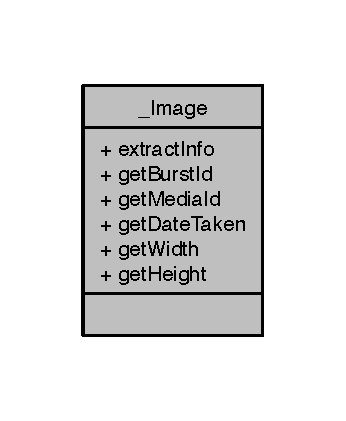
\includegraphics[width=166pt]{d1/d9b/struct__Image__coll__graph}
\end{center}
\end{figure}
\subsection*{Data Fields}
\begin{DoxyCompactItemize}
\item 
\hypertarget{struct__Image_abc38422f15a135e8d3d488fd17404a11}{bool($\ast$ {\bfseries extract\-Info} )(\hyperlink{struct__Image}{Image} this\-\_\-gen, String src)}\label{struct__Image_abc38422f15a135e8d3d488fd17404a11}

\item 
\hypertarget{struct__Image_a43ccbbf065326a2647887464f16b7373}{String($\ast$ {\bfseries get\-Burst\-Id} )(\hyperlink{struct__Image}{Image} this\-\_\-gen)}\label{struct__Image_a43ccbbf065326a2647887464f16b7373}

\item 
\hypertarget{struct__Image_a3ebc4a1fcad891955f6bd315dbf79b87}{String($\ast$ {\bfseries get\-Media\-Id} )(\hyperlink{struct__Image}{Image} this\-\_\-gen)}\label{struct__Image_a3ebc4a1fcad891955f6bd315dbf79b87}

\item 
\hypertarget{struct__Image_a170cc9a88ad9e65b2d8725d1370bc946}{String($\ast$ {\bfseries get\-Date\-Taken} )(\hyperlink{struct__Image}{Image} this\-\_\-gen)}\label{struct__Image_a170cc9a88ad9e65b2d8725d1370bc946}

\item 
\hypertarget{struct__Image_ac1af259a21d8c67dab2729dc2ca8e6ab}{int($\ast$ {\bfseries get\-Width} )(\hyperlink{struct__Image}{Image} this\-\_\-gen)}\label{struct__Image_ac1af259a21d8c67dab2729dc2ca8e6ab}

\item 
\hypertarget{struct__Image_a8958794ba1906035ca256305dc103399}{int($\ast$ {\bfseries get\-Height} )(\hyperlink{struct__Image}{Image} this\-\_\-gen)}\label{struct__Image_a8958794ba1906035ca256305dc103399}

\end{DoxyCompactItemize}


\subsection{Detailed Description}
Image 모듈에 대한 구조체이다. Image 모듈은 다양한 방식으로 동영상 파일을 제어 할 수 있다. 

\begin{DoxyNote}{Note}
File의 Image 모듈에 대한 구조체이다. \par
 구조체를 사용하기 전에 \hyperlink{File_8h_a8a073ef272f81217cf7a3665721970a7}{New\-Image()} 함수를 사용해야 하며 사용이 끝났을 때 \hyperlink{File_8h_a4dcf832a1b8f74b72f2fd59b99c53eb6}{Destroy\-Image()} 함수를 꼭 사용해야 한다. 
\end{DoxyNote}
\begin{DoxySeeAlso}{See Also}
\href{https://developer.tizen.org/dev-guide/2.3.0/org.tizen.native.mobile.apireference/group__CAPI__CONTENT__MEDIA__IMAGE__MODULE.html}{\tt https\-://developer.\-tizen.\-org/dev-\/guide/2.\-3.\-0/org.\-tizen.\-native.\-mobile.\-apireference/group\-\_\-\-\_\-\-C\-A\-P\-I\-\_\-\-\_\-\-C\-O\-N\-T\-E\-N\-T\-\_\-\-\_\-\-M\-E\-D\-I\-A\-\_\-\-\_\-\-I\-M\-A\-G\-E\-\_\-\-\_\-\-M\-O\-D\-U\-L\-E.\-html} 
\end{DoxySeeAlso}


Definition at line 555 of file File.\-h.



The documentation for this struct was generated from the following file\-:\begin{DoxyCompactItemize}
\item 
\hyperlink{File_8h}{File.\-h}\end{DoxyCompactItemize}

\section{Light Struct Reference}
\label{struct__Light}\index{Light@{Light}}


Light 모듈에 대한 구조체이다. Light 모듈은 Photometer Sensor를 다양한 방식으로 제어할 수 있다.  




{\ttfamily \#include $<$Sensor.\-h$>$}



Collaboration diagram for Light\-:\nopagebreak
\begin{figure}[H]
\begin{center}
\leavevmode
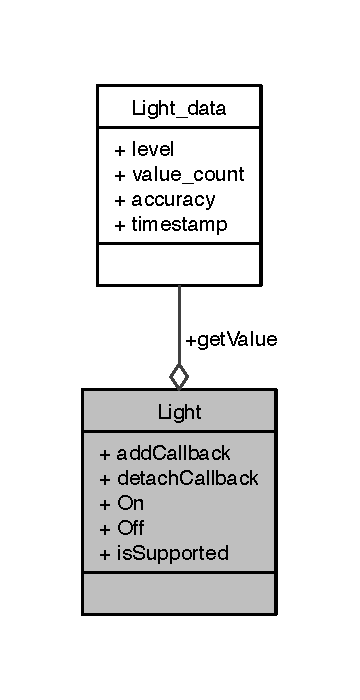
\includegraphics[width=173pt]{struct__Light__coll__graph}
\end{center}
\end{figure}
\subsection*{Data Fields}
\begin{DoxyCompactItemize}
\item 
bool($\ast$ {\bfseries add\-Callback} )(Light this\-\_\-gen, sensor\-\_\-callback sensor\-Callback, int timeinterval, void $\ast$data)\label{struct__Light_aeec1e6f6ea47e14947dd91d66fd2f228}

\item 
bool($\ast$ {\bfseries detach\-Callback} )(Light this\-\_\-gen)\label{struct__Light_a88fda56b990b88e192a9af894fae2271}

\item 
bool($\ast$ {\bfseries On} )(Light this\-\_\-gen)\label{struct__Light_a3ad693923f47b9b9e147f084f21c3dd3}

\item 
bool($\ast$ {\bfseries Off} )(Light this\-\_\-gen)\label{struct__Light_ac3aae8952fa68eb7f1245029157ab942}

\item 
bool($\ast$ {\bfseries is\-Supported} )(Light this\-\_\-gen)\label{struct__Light_a14f84ae58d7bca9de3236631eb8b50a8}

\item 
{\bf Light\-\_\-data}($\ast$ {\bfseries get\-Value} )(Light this\-\_\-gen)\label{struct__Light_ac57a94e478d6c653330a780e23ca600f}

\end{DoxyCompactItemize}


\subsection{Detailed Description}
Light 모듈에 대한 구조체이다. Light 모듈은 Photometer Sensor를 다양한 방식으로 제어할 수 있다. 

\begin{DoxyNote}{Note}
Light 모듈에 대한 구조체이다. \par
 구조체를 사용하기 전에 \doxyref{New\-Light()}{p.}{Sensor_8h_acc102a67ded8d183805b270f2e350dc3} 함수를 사용해야 하며 사용이 끝났을 때 \doxyref{Destroy\-Light()}{p.}{Sensor_8h_a8886d4cca6cda321936c1db6050f46c9} 함수를 꼭 사용해야 한다. 
\end{DoxyNote}
\begin{DoxySeeAlso}{See Also}
{\tt Tizen Native A\-P\-I Document -\/ Sensor part} 
\end{DoxySeeAlso}
\begin{DoxyPrecond}{Precondition}
{\bfseries feature} \par

\begin{DoxyItemize}
\item {\tt http\-://tizen.\-org/feature/sensor.\-photometer} 
\end{DoxyItemize}
\end{DoxyPrecond}


The documentation for this struct was generated from the following file\-:\begin{DoxyCompactItemize}
\item 
{\bf Sensor.\-h}\end{DoxyCompactItemize}

\hypertarget{struct__LinearAccelation}{\section{\-\_\-\-Linear\-Accelation Struct Reference}
\label{struct__LinearAccelation}\index{\-\_\-\-Linear\-Accelation@{\-\_\-\-Linear\-Accelation}}
}


Linear\-Accelation 모듈에 대한 구조체이다. Linear\-Accelation 모듈은 Linear\-Accelation Sensor를 다양한 방식으로 제어할 수 있다.  




{\ttfamily \#include $<$Sensor.\-h$>$}



Collaboration diagram for \-\_\-\-Linear\-Accelation\-:\nopagebreak
\begin{figure}[H]
\begin{center}
\leavevmode
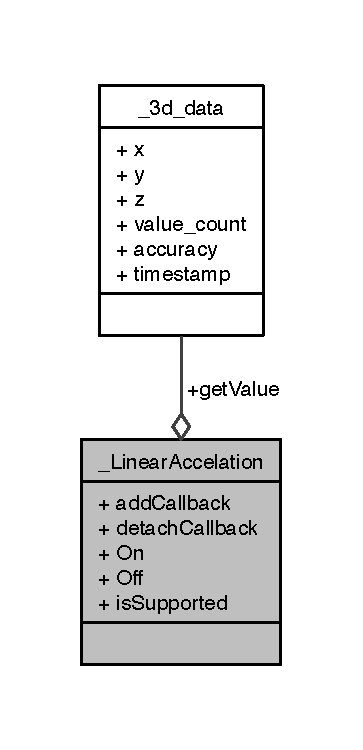
\includegraphics[width=174pt]{dd/d17/struct__LinearAccelation__coll__graph}
\end{center}
\end{figure}
\subsection*{Data Fields}
\begin{DoxyCompactItemize}
\item 
\hypertarget{struct__LinearAccelation_ae693a7f0650526be7b2439f650e811d5}{bool($\ast$ {\bfseries add\-Callback} )(\hyperlink{struct__LinearAccelation}{Linear\-Accelation} this\-\_\-gen, sensor\-\_\-callback sensor\-Callback, int timeinterval, void $\ast$data)}\label{struct__LinearAccelation_ae693a7f0650526be7b2439f650e811d5}

\item 
\hypertarget{struct__LinearAccelation_a8018bab15839a523647ae0eef1866403}{bool($\ast$ {\bfseries detach\-Callback} )(\hyperlink{struct__LinearAccelation}{Linear\-Accelation} this\-\_\-gen)}\label{struct__LinearAccelation_a8018bab15839a523647ae0eef1866403}

\item 
\hypertarget{struct__LinearAccelation_a4f1be3c71a431ac369f48cc7bdf4ab2e}{bool($\ast$ {\bfseries On} )(\hyperlink{struct__LinearAccelation}{Linear\-Accelation} this\-\_\-gen)}\label{struct__LinearAccelation_a4f1be3c71a431ac369f48cc7bdf4ab2e}

\item 
\hypertarget{struct__LinearAccelation_a117a2ff551470e568c61325a20047582}{bool($\ast$ {\bfseries Off} )(\hyperlink{struct__LinearAccelation}{Linear\-Accelation} this\-\_\-gen)}\label{struct__LinearAccelation_a117a2ff551470e568c61325a20047582}

\item 
\hypertarget{struct__LinearAccelation_afc42a6003589d08871b06adfc3f2ee9c}{bool($\ast$ {\bfseries is\-Supported} )(\hyperlink{struct__LinearAccelation}{Linear\-Accelation} this\-\_\-gen)}\label{struct__LinearAccelation_afc42a6003589d08871b06adfc3f2ee9c}

\item 
\hypertarget{struct__LinearAccelation_aaf02870c60aa510568b3376a4cd4d965}{\hyperlink{Sensor_8h_df/d29/struct__3d__data}{Linear\-Acceleration\-\_\-data}($\ast$ {\bfseries get\-Value} )(\hyperlink{struct__LinearAccelation}{Linear\-Accelation} this\-\_\-gen)}\label{struct__LinearAccelation_aaf02870c60aa510568b3376a4cd4d965}

\end{DoxyCompactItemize}


\subsection{Detailed Description}
Linear\-Accelation 모듈에 대한 구조체이다. Linear\-Accelation 모듈은 Linear\-Accelation Sensor를 다양한 방식으로 제어할 수 있다. 

\begin{DoxyNote}{Note}
Linear\-Accelation 모듈에 대한 구조체이다. \par
 구조체를 사용하기 전에 \hyperlink{Sensor_8h_aa7dc89111815a354e208a521a89936e9}{New\-Linear\-Accelation()} 함수를 사용해야 하며 사용이 끝났을 때 \hyperlink{Sensor_8h_a855b978e0631263963def31aa53c3545}{Destroy\-Linear\-Accelation()} 함수를 꼭 사용해야 한다. 
\end{DoxyNote}
\begin{DoxySeeAlso}{See Also}
\href{https://developer.tizen.org/dev-guide/2.3.0/org.tizen.native.mobile.apireference/group__CAPI__SYSTEM__SENSOR__MODULE.html}{\tt https\-://developer.\-tizen.\-org/dev-\/guide/2.\-3.\-0/org.\-tizen.\-native.\-mobile.\-apireference/group\-\_\-\-\_\-\-C\-A\-P\-I\-\_\-\-\_\-\-S\-Y\-S\-T\-E\-M\-\_\-\-\_\-\-S\-E\-N\-S\-O\-R\-\_\-\-\_\-\-M\-O\-D\-U\-L\-E.\-html} 
\end{DoxySeeAlso}


Definition at line 470 of file Sensor.\-h.



The documentation for this struct was generated from the following file\-:\begin{DoxyCompactItemize}
\item 
\hyperlink{Sensor_8h}{Sensor.\-h}\end{DoxyCompactItemize}

\hypertarget{struct__Magnetometer}{\section{\-\_\-\-Magnetometer Struct Reference}
\label{struct__Magnetometer}\index{\-\_\-\-Magnetometer@{\-\_\-\-Magnetometer}}
}


Magnetometer 모듈에 대한 구조체이다. Magnetometer 모듈은 Magnetometer Sensor를 다양한 방식으로 제어할 수 있다.  




{\ttfamily \#include $<$Sensor.\-h$>$}



Collaboration diagram for \-\_\-\-Magnetometer\-:\nopagebreak
\begin{figure}[H]
\begin{center}
\leavevmode
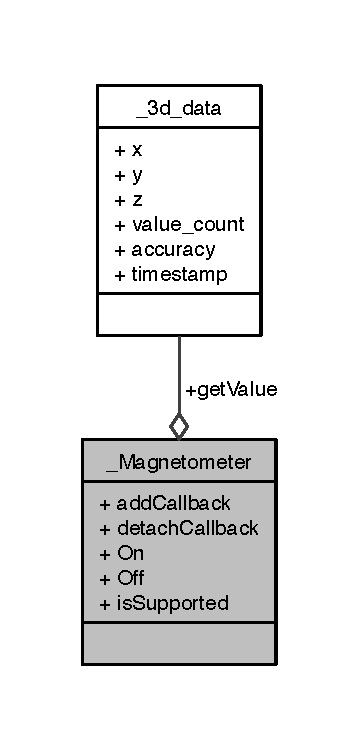
\includegraphics[width=173pt]{db/d36/struct__Magnetometer__coll__graph}
\end{center}
\end{figure}
\subsection*{Data Fields}
\begin{DoxyCompactItemize}
\item 
\hypertarget{struct__Magnetometer_aa97811d8ff97e63d37b695621c93ddd1}{bool($\ast$ {\bfseries add\-Callback} )(\hyperlink{struct__Magnetometer}{Magnetometer} this\-\_\-gen, sensor\-\_\-callback sensor\-Callback, int timeinterval, void $\ast$data)}\label{struct__Magnetometer_aa97811d8ff97e63d37b695621c93ddd1}

\item 
\hypertarget{struct__Magnetometer_a4af51e807baed6e87e3e6f7f509824e4}{bool($\ast$ {\bfseries detach\-Callback} )(\hyperlink{struct__Magnetometer}{Magnetometer} this\-\_\-gen)}\label{struct__Magnetometer_a4af51e807baed6e87e3e6f7f509824e4}

\item 
\hypertarget{struct__Magnetometer_aca82b27cfacc817306728b032909a7d5}{bool($\ast$ {\bfseries On} )(\hyperlink{struct__Magnetometer}{Magnetometer} this\-\_\-gen)}\label{struct__Magnetometer_aca82b27cfacc817306728b032909a7d5}

\item 
\hypertarget{struct__Magnetometer_ab987078b8057e016a32165087eb8fffc}{bool($\ast$ {\bfseries Off} )(\hyperlink{struct__Magnetometer}{Magnetometer} this\-\_\-gen)}\label{struct__Magnetometer_ab987078b8057e016a32165087eb8fffc}

\item 
\hypertarget{struct__Magnetometer_a1a1f2459baf385d09129335c806b66fe}{bool($\ast$ {\bfseries is\-Supported} )(\hyperlink{struct__Magnetometer}{Magnetometer} this\-\_\-gen)}\label{struct__Magnetometer_a1a1f2459baf385d09129335c806b66fe}

\item 
\hypertarget{struct__Magnetometer_a50494d12eb8d68827c7ea74b34dd2261}{\hyperlink{Sensor_8h_df/d29/struct__3d__data}{Magnetometer\-\_\-data}($\ast$ {\bfseries get\-Value} )(\hyperlink{struct__Magnetometer}{Magnetometer} this\-\_\-gen)}\label{struct__Magnetometer_a50494d12eb8d68827c7ea74b34dd2261}

\end{DoxyCompactItemize}


\subsection{Detailed Description}
Magnetometer 모듈에 대한 구조체이다. Magnetometer 모듈은 Magnetometer Sensor를 다양한 방식으로 제어할 수 있다. 

\begin{DoxyNote}{Note}
Magnetometer 모듈에 대한 구조체이다. \par
 구조체를 사용하기 전에 \hyperlink{Sensor_8h_ac0cc761c2c9b3872743da478e9c8b03a}{New\-Magnetometer()} 함수를 사용해야 하며 사용이 끝났을 때 \hyperlink{Sensor_8h_ade729513094ff7a9a2600b5389e346ac}{Destroy\-Magnetometer()} 함수를 꼭 사용해야 한다. 
\end{DoxyNote}
\begin{DoxySeeAlso}{See Also}
\href{https://developer.tizen.org/dev-guide/2.3.0/org.tizen.native.mobile.apireference/group__CAPI__SYSTEM__SENSOR__MODULE.html}{\tt https\-://developer.\-tizen.\-org/dev-\/guide/2.\-3.\-0/org.\-tizen.\-native.\-mobile.\-apireference/group\-\_\-\-\_\-\-C\-A\-P\-I\-\_\-\-\_\-\-S\-Y\-S\-T\-E\-M\-\_\-\-\_\-\-S\-E\-N\-S\-O\-R\-\_\-\-\_\-\-M\-O\-D\-U\-L\-E.\-html} 
\end{DoxySeeAlso}


Definition at line 645 of file Sensor.\-h.



The documentation for this struct was generated from the following file\-:\begin{DoxyCompactItemize}
\item 
\hyperlink{Sensor_8h}{Sensor.\-h}\end{DoxyCompactItemize}

\hypertarget{struct__NFC}{\section{\-\_\-\-N\-F\-C Struct Reference}
\label{struct__NFC}\index{\-\_\-\-N\-F\-C@{\-\_\-\-N\-F\-C}}
}


N\-F\-C모듈에 대한 구조체이다.  




{\ttfamily \#include $<$N\-F\-C.\-h$>$}



Collaboration diagram for \-\_\-\-N\-F\-C\-:\nopagebreak
\begin{figure}[H]
\begin{center}
\leavevmode
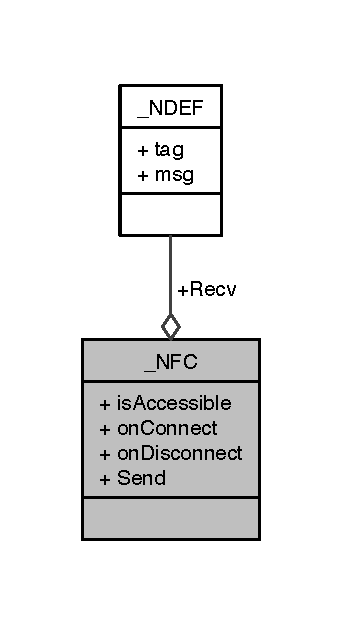
\includegraphics[width=164pt]{db/d89/struct__NFC__coll__graph}
\end{center}
\end{figure}
\subsection*{Data Fields}
\begin{DoxyCompactItemize}
\item 
\hypertarget{struct__NFC_ac1c45ebcef1f0a82a2bc140a9a2d572b}{bool($\ast$ {\bfseries is\-Accessible} )(\hyperlink{struct__NFC}{N\-F\-C} this\-\_\-gen)}\label{struct__NFC_ac1c45ebcef1f0a82a2bc140a9a2d572b}

\item 
\hypertarget{struct__NFC_a070219e871b65c63119b2b9fcf2f7e40}{bool($\ast$ {\bfseries on\-Connect} )(\hyperlink{struct__NFC}{N\-F\-C} this\-\_\-gen)}\label{struct__NFC_a070219e871b65c63119b2b9fcf2f7e40}

\item 
\hypertarget{struct__NFC_a3c638b599b78d063fd8472ea015597e0}{bool($\ast$ {\bfseries on\-Disconnect} )(\hyperlink{struct__NFC}{N\-F\-C} this\-\_\-gen)}\label{struct__NFC_a3c638b599b78d063fd8472ea015597e0}

\item 
\hypertarget{struct__NFC_a66682eb598e5e0ae8ab320f1e936f775}{bool($\ast$ {\bfseries Send} )(\hyperlink{struct__NFC}{N\-F\-C} this\-\_\-gen, \hyperlink{NFC_8h_d2/dce/struct__NDEF}{N\-D\-E\-F} message)}\label{struct__NFC_a66682eb598e5e0ae8ab320f1e936f775}

\item 
\hypertarget{struct__NFC_a2c24741e6d306b941e4b30559e5b7a52}{\hyperlink{NFC_8h_d2/dce/struct__NDEF}{N\-D\-E\-F}($\ast$ {\bfseries Recv} )(\hyperlink{struct__NFC}{N\-F\-C} this\-\_\-gen)}\label{struct__NFC_a2c24741e6d306b941e4b30559e5b7a52}

\end{DoxyCompactItemize}


\subsection{Detailed Description}
N\-F\-C모듈에 대한 구조체이다. 

\begin{DoxyNote}{Note}
N\-F\-C모듈에 대한 구조체이다. 구조체를 사용하기전에 \hyperlink{NFC_8h_a03b543f63bf7d41bb184db9209d5cc9c}{New\-N\-F\-C()} 함수를 사용 해야 하며 사용이 끝났을 때 \hyperlink{NFC_8h_a1e5dc8f957d33cd59f30e03f113d63fe}{Destroy\-N\-F\-C()}함수를 꼭 사용해야한다. 
\end{DoxyNote}
\begin{DoxySeeAlso}{See Also}
\href{https://developer.tizen.org/dev-guide/2.3.0/org.tizen.native.mobile.apireference/group__CAPI__NETWORK__NFC__MODULE.html}{\tt https\-://developer.\-tizen.\-org/dev-\/guide/2.\-3.\-0/org.\-tizen.\-native.\-mobile.\-apireference/group\-\_\-\-\_\-\-C\-A\-P\-I\-\_\-\-\_\-\-N\-E\-T\-W\-O\-R\-K\-\_\-\-\_\-\-N\-F\-C\-\_\-\-\_\-\-M\-O\-D\-U\-L\-E.\-html} 
\end{DoxySeeAlso}
\begin{DoxyPrecond}{Precondition}
features에 \char`\"{}http\-://tizen.\-org/feature/network.\-nfc\char`\"{} 를 추가해야 한다. 
\end{DoxyPrecond}


Definition at line 104 of file N\-F\-C.\-h.



The documentation for this struct was generated from the following file\-:\begin{DoxyCompactItemize}
\item 
\hyperlink{NFC_8h}{N\-F\-C.\-h}\end{DoxyCompactItemize}

\section{Notification Struct Reference}
\label{struct__Notification}\index{Notification@{Notification}}


Notification 모듈에 대한 구조체이다. Notification 모듈은 다양한 방식으로 알림을 설정 할 수 있다.  




{\ttfamily \#include $<$Notification.\-h$>$}



Collaboration diagram for Notification\-:\nopagebreak
\begin{figure}[H]
\begin{center}
\leavevmode
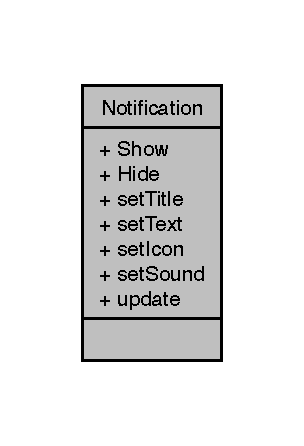
\includegraphics[width=146pt]{struct__Notification__coll__graph}
\end{center}
\end{figure}
\subsection*{Data Fields}
\begin{DoxyCompactItemize}
\item 
bool($\ast$ {\bfseries Show} )(Notification this\-\_\-gen)\label{struct__Notification_ab49ce2c6de39138bdeed864779f72a01}

\item 
bool($\ast$ {\bfseries Hide} )(Notification this\-\_\-gen)\label{struct__Notification_a924c840bdfa028ecff645aa4c9904ad9}

\item 
bool($\ast$ {\bfseries set\-Title} )(Notification this\-\_\-gen, String title)\label{struct__Notification_a5eb7a012d7a9f55dea3a10158bec5d19}

\item 
bool($\ast$ {\bfseries set\-Text} )(Notification this\-\_\-gen, String text)\label{struct__Notification_a52fc9be6dbfa7ca638c7c001a82c82e9}

\item 
bool($\ast$ {\bfseries set\-Icon} )(Notification this\-\_\-gen, String image\-Path)\label{struct__Notification_a7c293fca72b6ec788caf94542a906bc6}

\item 
bool($\ast$ {\bfseries set\-Sound} )(Notification this\-\_\-gen, String sound\-Path)\label{struct__Notification_ae47875a1c8bb2e6101c1601ab9c200bd}

\item 
bool($\ast$ {\bfseries update} )(Notification this\-\_\-gen)\label{struct__Notification_a8c9af5acbd17f0e8d15ee4bbbb1912cd}

\end{DoxyCompactItemize}


\subsection{Detailed Description}
Notification 모듈에 대한 구조체이다. Notification 모듈은 다양한 방식으로 알림을 설정 할 수 있다. 

\begin{DoxyNote}{Note}
Notification 모듈에 대한 구조체이다. \par
 구조체를 사용하기 전에 \doxyref{New\-Notification()}{p.}{Notification_8h_a404347c07b739823c244d09934047898} 함수를 사용해야 하며 사용이 끝났을 때 \doxyref{Destroy\-Notification()}{p.}{Notification_8h_a940d91a8e15dc9c5fd098c134842a326} 함수를 꼭 사용해야 한다. 
\end{DoxyNote}
\begin{DoxySeeAlso}{See Also}
{\tt Tizen Native A\-P\-I Document -\/ Notification part} 
\end{DoxySeeAlso}
\begin{DoxyPrecond}{Precondition}
{\bfseries privilege} \par

\begin{DoxyItemize}
\item {\tt http\-://tizen.\-org/privilege/notification} 
\end{DoxyItemize}
\end{DoxyPrecond}


The documentation for this struct was generated from the following file\-:\begin{DoxyCompactItemize}
\item 
{\bf Notification.\-h}\end{DoxyCompactItemize}

\section{Ongoing\-Notification Struct Reference}
\label{struct__OngoingNotification}\index{Ongoing\-Notification@{Ongoing\-Notification}}


Ongoing\-Notification 모듈에 대한 구조체이다. Ongoing\-Notification 모듈은 다양한 방식으로 알림을 설정 할 수 있다.  




{\ttfamily \#include $<$Ongoing\-Notification.\-h$>$}



Collaboration diagram for Ongoing\-Notification\-:\nopagebreak
\begin{figure}[H]
\begin{center}
\leavevmode
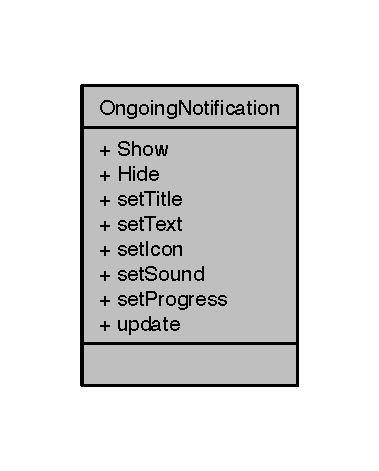
\includegraphics[width=182pt]{struct__OngoingNotification__coll__graph}
\end{center}
\end{figure}
\subsection*{Data Fields}
\begin{DoxyCompactItemize}
\item 
bool($\ast$ {\bfseries Show} )(Ongoing\-Notification this\-\_\-gen)\label{struct__OngoingNotification_aa21241d82ff53185630e4be0f97499d5}

\item 
bool($\ast$ {\bfseries Hide} )(Ongoing\-Notification this\-\_\-gen)\label{struct__OngoingNotification_a300d850ec8ec64944695b3d53b27b18e}

\item 
bool($\ast$ {\bfseries set\-Title} )(Ongoing\-Notification this\-\_\-gen, String title)\label{struct__OngoingNotification_af7c6b33a0a6fdb8ee98e2e0222388582}

\item 
bool($\ast$ {\bfseries set\-Text} )(Ongoing\-Notification this\-\_\-gen, String text)\label{struct__OngoingNotification_ac9c362dd4e9dea93c28e3692ec99f60c}

\item 
bool($\ast$ {\bfseries set\-Icon} )(Ongoing\-Notification this\-\_\-gen, String image\-Path)\label{struct__OngoingNotification_a0626b356e9ebaa9e9eae25bc3d3362c1}

\item 
bool($\ast$ {\bfseries set\-Sound} )(Ongoing\-Notification this\-\_\-gen, String sound\-Path)\label{struct__OngoingNotification_a6ee588fbcc8710d4e60024e0c5b44856}

\item 
bool($\ast$ {\bfseries set\-Progress} )(Ongoing\-Notification this\-\_\-gen, double progress)\label{struct__OngoingNotification_ad79a95e96a1a3645d03487ef48865412}

\item 
bool($\ast$ {\bfseries update} )(Ongoing\-Notification this\-\_\-gen)\label{struct__OngoingNotification_a9cd4eebab7558d84b6fb5f4999a8aa3b}

\end{DoxyCompactItemize}


\subsection{Detailed Description}
Ongoing\-Notification 모듈에 대한 구조체이다. Ongoing\-Notification 모듈은 다양한 방식으로 알림을 설정 할 수 있다. 

\begin{DoxyNote}{Note}
Ongoing\-Notification 모듈에 대한 구조체이다. \par
 구조체를 사용하기 전에 \doxyref{New\-Ongoing\-Notification()}{p.}{OngoingNotification_8h_a87a80dfbcb3f8f9bde6cfbd468dc2da3} 함수를 사용해야 하며 사용이 끝났을 때 \doxyref{Destroy\-Ongoing\-Notification()}{p.}{OngoingNotification_8h_a4368aefd18207753cebec1fffc8f5fc5} 함수를 꼭 사용해야 한다. 
\end{DoxyNote}
\begin{DoxySeeAlso}{See Also}
{\tt Tizen Native A\-P\-I Document -\/ Notification part} 
\end{DoxySeeAlso}
\begin{DoxyPrecond}{Precondition}
{\bfseries privilege} \par

\begin{DoxyItemize}
\item {\tt http\-://tizen.\-org/privilege/notification} 
\end{DoxyItemize}
\end{DoxyPrecond}


The documentation for this struct was generated from the following file\-:\begin{DoxyCompactItemize}
\item 
{\bf Ongoing\-Notification.\-h}\end{DoxyCompactItemize}

\hypertarget{struct__Orientation}{\section{\-\_\-\-Orientation Struct Reference}
\label{struct__Orientation}\index{\-\_\-\-Orientation@{\-\_\-\-Orientation}}
}


Orientation 모듈에 대한 구조체이다. Orientation 모듈은 Orientation Sensor를 다양한 방식으로 제어할 수 있다.  




{\ttfamily \#include $<$Sensor.\-h$>$}



Collaboration diagram for \-\_\-\-Orientation\-:\nopagebreak
\begin{figure}[H]
\begin{center}
\leavevmode
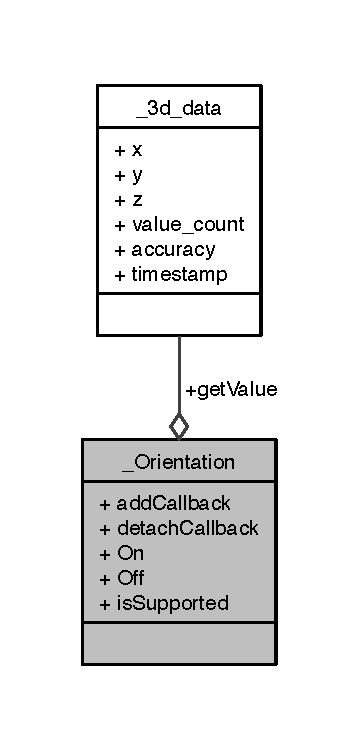
\includegraphics[width=173pt]{d5/dad/struct__Orientation__coll__graph}
\end{center}
\end{figure}
\subsection*{Data Fields}
\begin{DoxyCompactItemize}
\item 
\hypertarget{struct__Orientation_a62e2301d56463501b712969250de0b51}{bool($\ast$ {\bfseries add\-Callback} )(\hyperlink{struct__Orientation}{Orientation} this\-\_\-gen, sensor\-\_\-callback sensor\-Callback, int timeinterval, void $\ast$data)}\label{struct__Orientation_a62e2301d56463501b712969250de0b51}

\item 
\hypertarget{struct__Orientation_a5a0f426bae69f9f93d2455d65089084d}{bool($\ast$ {\bfseries detach\-Callback} )(\hyperlink{struct__Orientation}{Orientation} this\-\_\-gen)}\label{struct__Orientation_a5a0f426bae69f9f93d2455d65089084d}

\item 
\hypertarget{struct__Orientation_a1fdc91ded986983fc430dbb768964cf1}{bool($\ast$ {\bfseries On} )(\hyperlink{struct__Orientation}{Orientation} this\-\_\-gen)}\label{struct__Orientation_a1fdc91ded986983fc430dbb768964cf1}

\item 
\hypertarget{struct__Orientation_a5a8bf0f2c2a0508fb6ecf20731ae1965}{bool($\ast$ {\bfseries Off} )(\hyperlink{struct__Orientation}{Orientation} this\-\_\-gen)}\label{struct__Orientation_a5a8bf0f2c2a0508fb6ecf20731ae1965}

\item 
\hypertarget{struct__Orientation_af272be2847d4987b9107f4f016b573f1}{bool($\ast$ {\bfseries is\-Supported} )(\hyperlink{struct__Orientation}{Orientation} this\-\_\-gen)}\label{struct__Orientation_af272be2847d4987b9107f4f016b573f1}

\item 
\hypertarget{struct__Orientation_abb38457c67d18f412e911e5173d62419}{\hyperlink{Sensor_8h_df/d29/struct__3d__data}{Orientation\-\_\-data}($\ast$ {\bfseries get\-Value} )(\hyperlink{struct__Orientation}{Orientation} this\-\_\-gen)}\label{struct__Orientation_abb38457c67d18f412e911e5173d62419}

\end{DoxyCompactItemize}


\subsection{Detailed Description}
Orientation 모듈에 대한 구조체이다. Orientation 모듈은 Orientation Sensor를 다양한 방식으로 제어할 수 있다. 

\begin{DoxyNote}{Note}
Orientation 모듈에 대한 구조체이다. \par
 구조체를 사용하기 전에 \hyperlink{Sensor_8h_a12902ef31bcac8b287d775743c1b774d}{New\-Orientation()} 함수를 사용해야 하며 사용이 끝났을 때 \hyperlink{Sensor_8h_ab42d602375fb6943a8823543a349100a}{Destroy\-Orientation()} 함수를 꼭 사용해야 한다. 
\end{DoxyNote}
\begin{DoxySeeAlso}{See Also}
\href{https://developer.tizen.org/dev-guide/2.3.0/org.tizen.native.mobile.apireference/group__CAPI__SYSTEM__SENSOR__MODULE.html}{\tt https\-://developer.\-tizen.\-org/dev-\/guide/2.\-3.\-0/org.\-tizen.\-native.\-mobile.\-apireference/group\-\_\-\-\_\-\-C\-A\-P\-I\-\_\-\-\_\-\-S\-Y\-S\-T\-E\-M\-\_\-\-\_\-\-S\-E\-N\-S\-O\-R\-\_\-\-\_\-\-M\-O\-D\-U\-L\-E.\-html} 
\end{DoxySeeAlso}


Definition at line 995 of file Sensor.\-h.



The documentation for this struct was generated from the following file\-:\begin{DoxyCompactItemize}
\item 
\hyperlink{Sensor_8h}{Sensor.\-h}\end{DoxyCompactItemize}

\hypertarget{struct__Preference}{\section{\-\_\-\-Preference Struct Reference}
\label{struct__Preference}\index{\-\_\-\-Preference@{\-\_\-\-Preference}}
}


Preference 모듈에 대한 구조체이다. Preference 모듈은 다양한 형식으로 key값을 제어 할 수 있다.  




{\ttfamily \#include $<$Preference.\-h$>$}



Collaboration diagram for \-\_\-\-Preference\-:\nopagebreak
\begin{figure}[H]
\begin{center}
\leavevmode
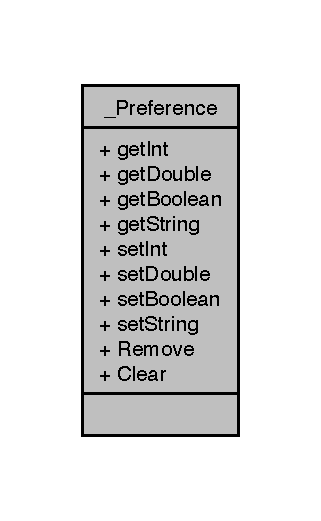
\includegraphics[width=154pt]{d5/d04/struct__Preference__coll__graph}
\end{center}
\end{figure}
\subsection*{Data Fields}
\begin{DoxyCompactItemize}
\item 
\hypertarget{struct__Preference_a354ae0d851333f72a06ea51e0bcb8360}{int($\ast$ {\bfseries get\-Int} )(String key, int def\-Value)}\label{struct__Preference_a354ae0d851333f72a06ea51e0bcb8360}

\item 
\hypertarget{struct__Preference_a96f41840c325a881dc63177979b83b52}{double($\ast$ {\bfseries get\-Double} )(String key, double def\-Value)}\label{struct__Preference_a96f41840c325a881dc63177979b83b52}

\item 
\hypertarget{struct__Preference_a32b9944e22dd04233008ebc1afba21c8}{bool($\ast$ {\bfseries get\-Boolean} )(String key, bool def\-Value)}\label{struct__Preference_a32b9944e22dd04233008ebc1afba21c8}

\item 
\hypertarget{struct__Preference_ab43532513cb470d242f06a41c90c2320}{String($\ast$ {\bfseries get\-String} )(String key, String def\-Value)}\label{struct__Preference_ab43532513cb470d242f06a41c90c2320}

\item 
\hypertarget{struct__Preference_a6417c5ebd12f4db875a6cd38ef44be02}{bool($\ast$ {\bfseries set\-Int} )(String key, int value)}\label{struct__Preference_a6417c5ebd12f4db875a6cd38ef44be02}

\item 
\hypertarget{struct__Preference_a0d0e596ceb6c5a3550393ccef4c75ae2}{bool($\ast$ {\bfseries set\-Double} )(String key, double value)}\label{struct__Preference_a0d0e596ceb6c5a3550393ccef4c75ae2}

\item 
\hypertarget{struct__Preference_a485c55e39fd4e98f77330a0db4cb7356}{bool($\ast$ {\bfseries set\-Boolean} )(String key, bool value)}\label{struct__Preference_a485c55e39fd4e98f77330a0db4cb7356}

\item 
\hypertarget{struct__Preference_af78be25d0215f85c626cbc4743622b09}{bool($\ast$ {\bfseries set\-String} )(String key, String value)}\label{struct__Preference_af78be25d0215f85c626cbc4743622b09}

\item 
\hypertarget{struct__Preference_a7edaf50caa291810d8f0ece33aa870a4}{bool($\ast$ {\bfseries Remove} )(String key)}\label{struct__Preference_a7edaf50caa291810d8f0ece33aa870a4}

\item 
\hypertarget{struct__Preference_a52f04c61197aaf2ff41e083fcd140bf6}{bool($\ast$ {\bfseries Clear} )()}\label{struct__Preference_a52f04c61197aaf2ff41e083fcd140bf6}

\end{DoxyCompactItemize}


\subsection{Detailed Description}
Preference 모듈에 대한 구조체이다. Preference 모듈은 다양한 형식으로 key값을 제어 할 수 있다. 

\begin{DoxyNote}{Note}
Preference 모듈에 대한 구조체이다. \par
 구조체를 사용하기 전에 \hyperlink{Preference_8h_ac230ae82d235023850371be1c8e281fb}{New\-Preference()} 함수를 사용해야 하며 사용이 끝났을 때 \hyperlink{Preference_8h_afb9b36e8c53758ed9f012b907e1a17c4}{Destroy\-Preference()} 함수를 꼭 사용해야 한다. 
\end{DoxyNote}
\begin{DoxySeeAlso}{See Also}
\href{https://developer.tizen.org/dev-guide/2.3.0/org.tizen.native.mobile.apireference/group__CAPI__PREFERENCE__MODULE.html}{\tt https\-://developer.\-tizen.\-org/dev-\/guide/2.\-3.\-0/org.\-tizen.\-native.\-mobile.\-apireference/group\-\_\-\-\_\-\-C\-A\-P\-I\-\_\-\-\_\-\-P\-R\-E\-F\-E\-R\-E\-N\-C\-E\-\_\-\-\_\-\-M\-O\-D\-U\-L\-E.\-html} 
\end{DoxySeeAlso}


Definition at line 46 of file Preference.\-h.



The documentation for this struct was generated from the following file\-:\begin{DoxyCompactItemize}
\item 
\hyperlink{Preference_8h}{Preference.\-h}\end{DoxyCompactItemize}

\hypertarget{struct__Pressure}{\section{\-\_\-\-Pressure Struct Reference}
\label{struct__Pressure}\index{\-\_\-\-Pressure@{\-\_\-\-Pressure}}
}


Pressure 모듈에 대한 구조체이다. Pressure 모듈은 Pressure Sensor를 다양한 방식으로 제어할 수 있다.  




{\ttfamily \#include $<$Sensor.\-h$>$}



Collaboration diagram for \-\_\-\-Pressure\-:\nopagebreak
\begin{figure}[H]
\begin{center}
\leavevmode
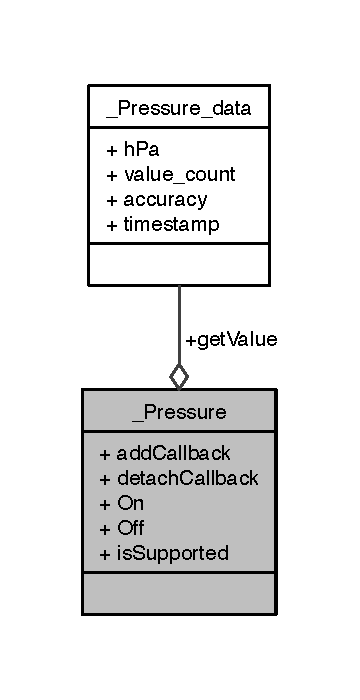
\includegraphics[width=173pt]{d8/df1/struct__Pressure__coll__graph}
\end{center}
\end{figure}
\subsection*{Data Fields}
\begin{DoxyCompactItemize}
\item 
\hypertarget{struct__Pressure_a34f0a13161a6d73a82b9cae7319ddf50}{bool($\ast$ {\bfseries add\-Callback} )(\hyperlink{struct__Pressure}{Pressure} this\-\_\-gen, sensor\-\_\-callback sensor\-Callback, int timeinterval, void $\ast$data)}\label{struct__Pressure_a34f0a13161a6d73a82b9cae7319ddf50}

\item 
\hypertarget{struct__Pressure_a7345c6a3cb4c89f7c1d8c7d8bdb91e80}{bool($\ast$ {\bfseries detach\-Callback} )(\hyperlink{struct__Pressure}{Pressure} this\-\_\-gen)}\label{struct__Pressure_a7345c6a3cb4c89f7c1d8c7d8bdb91e80}

\item 
\hypertarget{struct__Pressure_a76a894862d359f094d24add3cabae5ea}{bool($\ast$ {\bfseries On} )(\hyperlink{struct__Pressure}{Pressure} this\-\_\-gen)}\label{struct__Pressure_a76a894862d359f094d24add3cabae5ea}

\item 
\hypertarget{struct__Pressure_a30cf8913cc8a1712dc76eff8a73ced94}{bool($\ast$ {\bfseries Off} )(\hyperlink{struct__Pressure}{Pressure} this\-\_\-gen)}\label{struct__Pressure_a30cf8913cc8a1712dc76eff8a73ced94}

\item 
\hypertarget{struct__Pressure_af2099f6f9efc1f7213acfd420ea7b8c6}{bool($\ast$ {\bfseries is\-Supported} )(\hyperlink{struct__Pressure}{Pressure} this\-\_\-gen)}\label{struct__Pressure_af2099f6f9efc1f7213acfd420ea7b8c6}

\item 
\hypertarget{struct__Pressure_a9739a7d1b596639f720e0fbb2dd8f064}{\hyperlink{Sensor_8h_d4/dbb/struct__Pressure__data}{Pressure\-\_\-data}($\ast$ {\bfseries get\-Value} )(\hyperlink{struct__Pressure}{Pressure} this\-\_\-gen)}\label{struct__Pressure_a9739a7d1b596639f720e0fbb2dd8f064}

\end{DoxyCompactItemize}


\subsection{Detailed Description}
Pressure 모듈에 대한 구조체이다. Pressure 모듈은 Pressure Sensor를 다양한 방식으로 제어할 수 있다. 

\begin{DoxyNote}{Note}
Pressure 모듈에 대한 구조체이다. \par
 구조체를 사용하기 전에 \hyperlink{Sensor_8h_ae9affb62208c3fa0cd182163c2447cb0}{New\-Pressure()} 함수를 사용해야 하며 사용이 끝났을 때 \hyperlink{Sensor_8h_af30fd514c8a87224bc535116633bbba3}{Destroy\-Pressure()} 함수를 꼭 사용해야 한다. 
\end{DoxyNote}
\begin{DoxySeeAlso}{See Also}
\href{https://developer.tizen.org/dev-guide/2.3.0/org.tizen.native.mobile.apireference/group__CAPI__SYSTEM__SENSOR__MODULE.html}{\tt https\-://developer.\-tizen.\-org/dev-\/guide/2.\-3.\-0/org.\-tizen.\-native.\-mobile.\-apireference/group\-\_\-\-\_\-\-C\-A\-P\-I\-\_\-\-\_\-\-S\-Y\-S\-T\-E\-M\-\_\-\-\_\-\-S\-E\-N\-S\-O\-R\-\_\-\-\_\-\-M\-O\-D\-U\-L\-E.\-html} 
\end{DoxySeeAlso}


Definition at line 1704 of file Sensor.\-h.



The documentation for this struct was generated from the following file\-:\begin{DoxyCompactItemize}
\item 
\hyperlink{Sensor_8h}{Sensor.\-h}\end{DoxyCompactItemize}

\hypertarget{struct__Proximity}{\section{\-\_\-\-Proximity Struct Reference}
\label{struct__Proximity}\index{\-\_\-\-Proximity@{\-\_\-\-Proximity}}
}


Proximity 모듈에 대한 구조체이다. Proximity 모듈은 Proximity Sensor를 다양한 방식으로 제어할 수 있다.  




{\ttfamily \#include $<$Sensor.\-h$>$}



Collaboration diagram for \-\_\-\-Proximity\-:\nopagebreak
\begin{figure}[H]
\begin{center}
\leavevmode
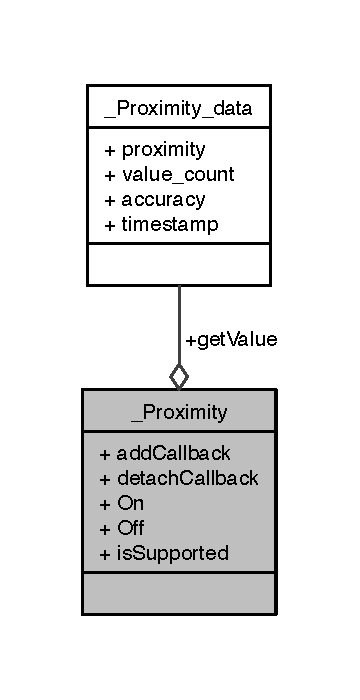
\includegraphics[width=173pt]{db/df8/struct__Proximity__coll__graph}
\end{center}
\end{figure}
\subsection*{Data Fields}
\begin{DoxyCompactItemize}
\item 
\hypertarget{struct__Proximity_a34233b2c53cafa32a16fee93bc87ee4d}{bool($\ast$ {\bfseries add\-Callback} )(\hyperlink{struct__Proximity}{Proximity} this\-\_\-gen, sensor\-\_\-callback sensor\-Callback, int timeinterval, void $\ast$data)}\label{struct__Proximity_a34233b2c53cafa32a16fee93bc87ee4d}

\item 
\hypertarget{struct__Proximity_ae3b089dbc605cca6672de861f726299d}{bool($\ast$ {\bfseries detach\-Callback} )(\hyperlink{struct__Proximity}{Proximity} this\-\_\-gen)}\label{struct__Proximity_ae3b089dbc605cca6672de861f726299d}

\item 
\hypertarget{struct__Proximity_a430c35da418a70bf04d59918d117c855}{bool($\ast$ {\bfseries On} )(\hyperlink{struct__Proximity}{Proximity} this\-\_\-gen)}\label{struct__Proximity_a430c35da418a70bf04d59918d117c855}

\item 
\hypertarget{struct__Proximity_a387e00eb751ec2969828e147580cf074}{bool($\ast$ {\bfseries Off} )(\hyperlink{struct__Proximity}{Proximity} this\-\_\-gen)}\label{struct__Proximity_a387e00eb751ec2969828e147580cf074}

\item 
\hypertarget{struct__Proximity_adfb2002e855b02ccf6f3dbcd636723ea}{bool($\ast$ {\bfseries is\-Supported} )(\hyperlink{struct__Proximity}{Proximity} this\-\_\-gen)}\label{struct__Proximity_adfb2002e855b02ccf6f3dbcd636723ea}

\item 
\hypertarget{struct__Proximity_abf3276a84c1e43e8e5ff5ecb6c665ee1}{\hyperlink{Sensor_8h_db/d98/struct__Proximity__data}{Proximity\-\_\-data}($\ast$ {\bfseries get\-Value} )(\hyperlink{struct__Proximity}{Proximity} this\-\_\-gen)}\label{struct__Proximity_abf3276a84c1e43e8e5ff5ecb6c665ee1}

\end{DoxyCompactItemize}


\subsection{Detailed Description}
Proximity 모듈에 대한 구조체이다. Proximity 모듈은 Proximity Sensor를 다양한 방식으로 제어할 수 있다. 

\begin{DoxyNote}{Note}
Proximity 모듈에 대한 구조체이다. \par
 구조체를 사용하기 전에 \hyperlink{Sensor_8h_adb707c0710a6913565dda16b69559940}{New\-Proximity()} 함수를 사용해야 하며 사용이 끝났을 때 \hyperlink{Sensor_8h_a826d9c3073df9e3332c8f6110bb3f991}{Destroy\-Proximity()} 함수를 꼭 사용해야 한다. 
\end{DoxyNote}
\begin{DoxySeeAlso}{See Also}
\href{https://developer.tizen.org/dev-guide/2.3.0/org.tizen.native.mobile.apireference/group__CAPI__SYSTEM__SENSOR__MODULE.html}{\tt https\-://developer.\-tizen.\-org/dev-\/guide/2.\-3.\-0/org.\-tizen.\-native.\-mobile.\-apireference/group\-\_\-\-\_\-\-C\-A\-P\-I\-\_\-\-\_\-\-S\-Y\-S\-T\-E\-M\-\_\-\-\_\-\-S\-E\-N\-S\-O\-R\-\_\-\-\_\-\-M\-O\-D\-U\-L\-E.\-html} 
\end{DoxySeeAlso}


Definition at line 1529 of file Sensor.\-h.



The documentation for this struct was generated from the following file\-:\begin{DoxyCompactItemize}
\item 
\hyperlink{Sensor_8h}{Sensor.\-h}\end{DoxyCompactItemize}

\section{Rotation\-Vector Struct Reference}
\label{struct__RotationVector}\index{Rotation\-Vector@{Rotation\-Vector}}


Rotation\-Vector 모듈에 대한 구조체이다. Rotation\-Vector 모듈은 Rotation\-Vector Sensor를 다양한 방식으로 제어할 수 있다.  




{\ttfamily \#include $<$Sensor.\-h$>$}



Collaboration diagram for Rotation\-Vector\-:\nopagebreak
\begin{figure}[H]
\begin{center}
\leavevmode
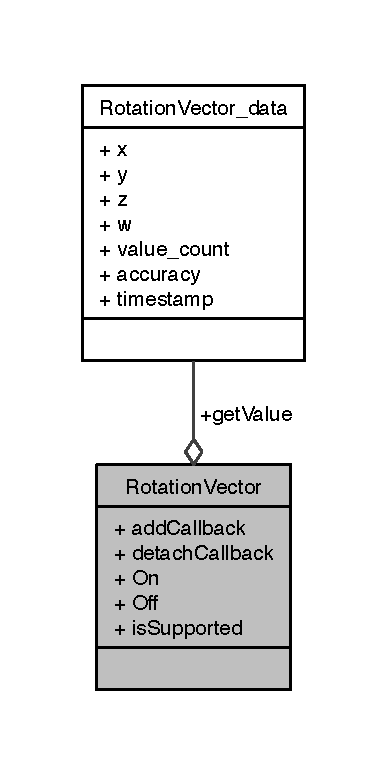
\includegraphics[width=186pt]{struct__RotationVector__coll__graph}
\end{center}
\end{figure}
\subsection*{Data Fields}
\begin{DoxyCompactItemize}
\item 
bool($\ast$ {\bfseries add\-Callback} )(Rotation\-Vector this\-\_\-gen, sensor\-\_\-callback sensor\-Callback, int timeinterval, void $\ast$data)\label{struct__RotationVector_a5c7c1ef26d4066e4b168ad0bdaa87c9c}

\item 
bool($\ast$ {\bfseries detach\-Callback} )(Rotation\-Vector this\-\_\-gen)\label{struct__RotationVector_ad95cf3aeadc994d223c58108b4c18521}

\item 
bool($\ast$ {\bfseries On} )(Rotation\-Vector this\-\_\-gen)\label{struct__RotationVector_a6c4bab80ab480bd0cb338a7b516290cc}

\item 
bool($\ast$ {\bfseries Off} )(Rotation\-Vector this\-\_\-gen)\label{struct__RotationVector_ac237d7751564daacd203f589c2da277a}

\item 
bool($\ast$ {\bfseries is\-Supported} )(Rotation\-Vector this\-\_\-gen)\label{struct__RotationVector_a461da1063b0477549abb8f3eb27e771a}

\item 
{\bf Rotation\-Vector\-\_\-data}($\ast$ {\bfseries get\-Value} )(Rotation\-Vector this\-\_\-gen)\label{struct__RotationVector_ab9137dff6865eb8ede19ef67318fdb26}

\end{DoxyCompactItemize}


\subsection{Detailed Description}
Rotation\-Vector 모듈에 대한 구조체이다. Rotation\-Vector 모듈은 Rotation\-Vector Sensor를 다양한 방식으로 제어할 수 있다. 

\begin{DoxyNote}{Note}
Rotation\-Vector 모듈에 대한 구조체이다. \par
 구조체를 사용하기 전에 \doxyref{New\-Rotation\-Vector()}{p.}{Sensor_8h_a5feb892af05fc21bb647dd0203ce384e} 함수를 사용해야 하며 사용이 끝났을 때 \doxyref{Destroy\-Rotation\-Vector()}{p.}{Sensor_8h_a88e94d5f3af20819de0f97b12f5435b1} 함수를 꼭 사용해야 한다. 
\end{DoxyNote}
\begin{DoxySeeAlso}{See Also}
{\tt Tizen Native A\-P\-I Document -\/ Sensor part} 
\end{DoxySeeAlso}
\begin{DoxyPrecond}{Precondition}
{\bfseries feature} \par

\begin{DoxyItemize}
\item {\tt http\-://tizen.\-org/feature/sensor.\-rotation\-\_\-vector} 
\end{DoxyItemize}
\end{DoxyPrecond}


The documentation for this struct was generated from the following file\-:\begin{DoxyCompactItemize}
\item 
{\bf Sensor.\-h}\end{DoxyCompactItemize}

\section{Socket Struct Reference}
\label{struct__Socket}\index{Socket@{Socket}}


Socket 모듈에 대한 구조체이다. Socket 모듈은 다양한 방식으로 Socket 통신을 할 수 있다.  




{\ttfamily \#include $<$Socket.\-h$>$}



Collaboration diagram for Socket\-:
\nopagebreak
\begin{figure}[H]
\begin{center}
\leavevmode
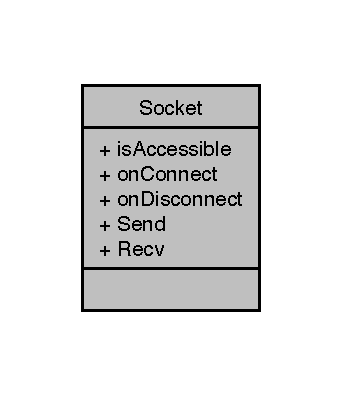
\includegraphics[width=164pt]{struct__Socket__coll__graph}
\end{center}
\end{figure}
\subsection*{Data Fields}
\begin{DoxyCompactItemize}
\item 
bool($\ast$ {\bfseries is\-Accessible} )(Socket this\-\_\-gen)\label{struct__Socket_ad4fe5e4e28f39180d8fe7e3fba9a1500}

\item 
bool($\ast$ {\bfseries on\-Connect} )(Socket this\-\_\-gen, String url, int port)\label{struct__Socket_aff2e54781fdd8d197c2eab035c32f309}

\item 
bool($\ast$ {\bfseries on\-Disconnect} )(Socket this\-\_\-gen)\label{struct__Socket_aed19956aa5326ac658b93c41e4a2f2e3}

\item 
bool($\ast$ {\bfseries Send} )(Socket this\-\_\-gen, String msg)\label{struct__Socket_a305bd4bc5e03c6de0586b2272fbc5982}

\item 
bool($\ast$ {\bfseries Recv} )(Socket this\-\_\-gen, String $\ast$msg)\label{struct__Socket_ad30b5d10747a9de59cfdf097447e2a65}

\end{DoxyCompactItemize}


\subsection{Detailed Description}
Socket 모듈에 대한 구조체이다. Socket 모듈은 다양한 방식으로 Socket 통신을 할 수 있다. 

\begin{DoxyNote}{Note}
Socket의 Socket 모듈에 대한 구조체이다. \par
 구조체를 사용하기 전에 \doxyref{New\-Socket()}{p.}{Socket_8h_a1e1d2bbe80adb61014a4a67b3b507aae} 함수를 사용해야 하며 사용이 끝났을 때 \doxyref{Destory\-Socket()}{p.}{Socket_8h_a72ff91c23eed60f629fbae39dbce94e2} 함수를 꼭 사용해야 한다. 
\end{DoxyNote}
\begin{DoxySeeAlso}{See Also}
{\tt Tizen Native A\-P\-I Document -\/ C\-U\-R\-L part} 
\end{DoxySeeAlso}
\begin{DoxyPrecond}{Precondition}
{\bfseries privilege} \par

\begin{DoxyItemize}
\item {\tt http\-://tizen.\-org/privilege/internet} 
\end{DoxyItemize}
\end{DoxyPrecond}


The documentation for this struct was generated from the following file\-:\begin{DoxyCompactItemize}
\item 
{\bf Socket.\-h}\end{DoxyCompactItemize}

\section{Temperature Struct Reference}
\label{struct__Temperature}\index{Temperature@{Temperature}}


Temperature 모듈에 대한 구조체이다. Temperature 모듈은 Temperature Sensor를 다양한 방식으로 제어할 수 있다.  




{\ttfamily \#include $<$Sensor.\-h$>$}



Collaboration diagram for Temperature\-:
\nopagebreak
\begin{figure}[H]
\begin{center}
\leavevmode
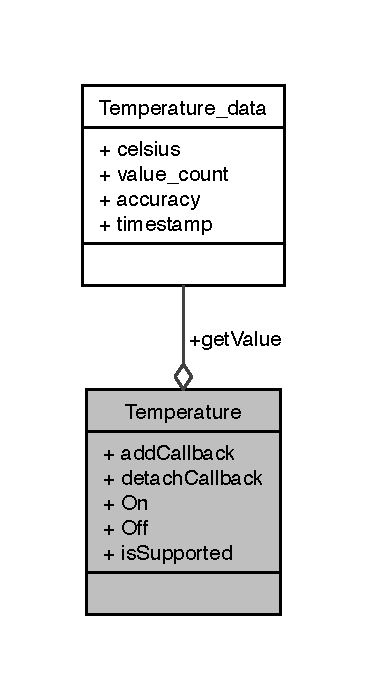
\includegraphics[width=176pt]{struct__Temperature__coll__graph}
\end{center}
\end{figure}
\subsection*{Data Fields}
\begin{DoxyCompactItemize}
\item 
bool($\ast$ {\bfseries add\-Callback} )(Temperature this\-\_\-gen, sensor\-\_\-callback sensor\-Callback, int timeinterval, void $\ast$data)\label{struct__Temperature_ae42650b42a974f34ab33f3cf50741f7a}

\item 
bool($\ast$ {\bfseries detach\-Callback} )(Temperature this\-\_\-gen)\label{struct__Temperature_a1528ad56ee1074d3a450dd26539cc2c5}

\item 
bool($\ast$ {\bfseries On} )(Temperature this\-\_\-gen)\label{struct__Temperature_a1e4f2d11cf25d437b746cc165dd1ff7b}

\item 
bool($\ast$ {\bfseries Off} )(Temperature this\-\_\-gen)\label{struct__Temperature_a6941ec5e6f840402b39f3dbdd12396e6}

\item 
bool($\ast$ {\bfseries is\-Supported} )(Temperature this\-\_\-gen)\label{struct__Temperature_a956fc3dcba797854840a1075fed89a92}

\item 
{\bf Temperature\-\_\-data}($\ast$ {\bfseries get\-Value} )(Temperature this\-\_\-gen)\label{struct__Temperature_ab2698eb90ec24a33a4c7675fd0ff7665}

\end{DoxyCompactItemize}


\subsection{Detailed Description}
Temperature 모듈에 대한 구조체이다. Temperature 모듈은 Temperature Sensor를 다양한 방식으로 제어할 수 있다. 

\begin{DoxyNote}{Note}
Temperature 모듈에 대한 구조체이다. \par
 구조체를 사용하기 전에 \doxyref{New\-Temperature()}{p.}{Sensor_8h_afd32f5f2a72ba185361018d8f2b450f7} 함수를 사용해야 하며 사용이 끝났을 때 \doxyref{Destroy\-Temperature()}{p.}{Sensor_8h_a31db7bd04fb88393523fe985fe007023} 함수를 꼭 사용해야 한다. 
\end{DoxyNote}
\begin{DoxySeeAlso}{See Also}
{\tt Tizen Native A\-P\-I Document -\/ Sensor part} 
\end{DoxySeeAlso}
\begin{DoxyPrecond}{Precondition}
{\bfseries feature} \par

\begin{DoxyItemize}
\item {\tt http\-://tizen.\-org/feature/sensor.\-temperature} 
\end{DoxyItemize}
\end{DoxyPrecond}


The documentation for this struct was generated from the following file\-:\begin{DoxyCompactItemize}
\item 
{\bf Sensor.\-h}\end{DoxyCompactItemize}

\section{Ultra\-Violet Struct Reference}
\label{struct__UltraViolet}\index{Ultra\-Violet@{Ultra\-Violet}}


Ultra\-Violet 모듈에 대한 구조체이다. Ultra\-Violet 모듈은 Ultra\-Violet Sensor를 다양한 방식으로 제어할 수 있다.  




{\ttfamily \#include $<$Sensor.\-h$>$}



Collaboration diagram for Ultra\-Violet\-:
\nopagebreak
\begin{figure}[H]
\begin{center}
\leavevmode
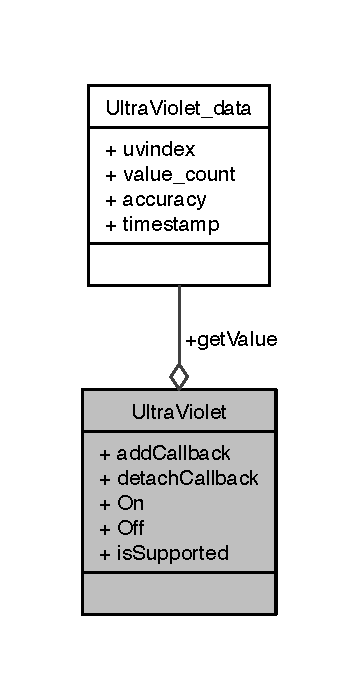
\includegraphics[width=173pt]{struct__UltraViolet__coll__graph}
\end{center}
\end{figure}
\subsection*{Data Fields}
\begin{DoxyCompactItemize}
\item 
bool($\ast$ {\bfseries add\-Callback} )(Ultra\-Violet this\-\_\-gen, sensor\-\_\-callback sensor\-Callback, int timeinterval, void $\ast$data)\label{struct__UltraViolet_a6f618f6eb746c4c6b36d2960eb51ca66}

\item 
bool($\ast$ {\bfseries detach\-Callback} )(Ultra\-Violet this\-\_\-gen)\label{struct__UltraViolet_ac9849529c808a351a56f552a6df0bc07}

\item 
bool($\ast$ {\bfseries On} )(Ultra\-Violet this\-\_\-gen)\label{struct__UltraViolet_ad6f214badc46556c865bec0f5c1195c9}

\item 
bool($\ast$ {\bfseries Off} )(Ultra\-Violet this\-\_\-gen)\label{struct__UltraViolet_ab5453dd539e93e0142669b39146963bb}

\item 
bool($\ast$ {\bfseries is\-Supported} )(Ultra\-Violet this\-\_\-gen)\label{struct__UltraViolet_af1f290e0f1cdf4f1389f9d64eab58804}

\item 
{\bf Ultra\-Violet\-\_\-data}($\ast$ {\bfseries get\-Value} )(Ultra\-Violet this\-\_\-gen)\label{struct__UltraViolet_a01b25572f437f19b612cf7953b575313}

\end{DoxyCompactItemize}


\subsection{Detailed Description}
Ultra\-Violet 모듈에 대한 구조체이다. Ultra\-Violet 모듈은 Ultra\-Violet Sensor를 다양한 방식으로 제어할 수 있다. 

\begin{DoxyNote}{Note}
Ultra\-Violet 모듈에 대한 구조체이다. \par
 구조체를 사용하기 전에 \doxyref{New\-Ultra\-Violet()}{p.}{Sensor_8h_a7bd9a5544d00f631a0e617b332f0b032} 함수를 사용해야 하며 사용이 끝났을 때 \doxyref{Destroy\-Ultra\-Violet()}{p.}{Sensor_8h_a42bd8c6715137f5fd8892667fe232c5c} 함수를 꼭 사용해야 한다. 
\end{DoxyNote}
\begin{DoxySeeAlso}{See Also}
{\tt Tizen Native A\-P\-I Document -\/ Sensor part} 
\end{DoxySeeAlso}
\begin{DoxyPrecond}{Precondition}
{\bfseries feature} \par

\begin{DoxyItemize}
\item {\tt http\-://tizen.\-org/feature/sensor.\-ultraviolet} 
\end{DoxyItemize}
\end{DoxyPrecond}


The documentation for this struct was generated from the following file\-:\begin{DoxyCompactItemize}
\item 
{\bf Sensor.\-h}\end{DoxyCompactItemize}

\hypertarget{struct__Vibration}{\section{\-\_\-\-Vibration Struct Reference}
\label{struct__Vibration}\index{\-\_\-\-Vibration@{\-\_\-\-Vibration}}
}


Vibration 모듈에 대한 구조체이다. Vibration 모듈은 다양한 방식으로 진동을 조절 할 수 있다.  




{\ttfamily \#include $<$Device\-Status.\-h$>$}



Collaboration diagram for \-\_\-\-Vibration\-:\nopagebreak
\begin{figure}[H]
\begin{center}
\leavevmode
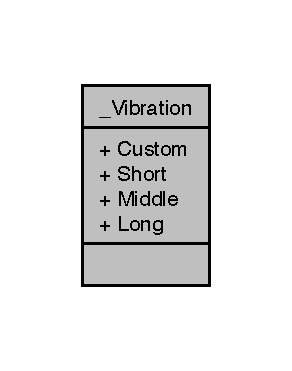
\includegraphics[width=140pt]{d6/d45/struct__Vibration__coll__graph}
\end{center}
\end{figure}
\subsection*{Data Fields}
\begin{DoxyCompactItemize}
\item 
\hypertarget{struct__Vibration_a1e609bae048cc8d21ad4e2eb03dc70d2}{bool($\ast$ {\bfseries Custom} )(\hyperlink{struct__Vibration}{Vibration} this\-\_\-gen, int period)}\label{struct__Vibration_a1e609bae048cc8d21ad4e2eb03dc70d2}

\item 
\hypertarget{struct__Vibration_a6df62054739bf6fdb04f6014b5a721b3}{bool($\ast$ {\bfseries Short} )(\hyperlink{struct__Vibration}{Vibration} this\-\_\-gen)}\label{struct__Vibration_a6df62054739bf6fdb04f6014b5a721b3}

\item 
\hypertarget{struct__Vibration_a524fb3aaeea4a2f0fc1b15127621de0f}{bool($\ast$ {\bfseries Middle} )(\hyperlink{struct__Vibration}{Vibration} this\-\_\-gen)}\label{struct__Vibration_a524fb3aaeea4a2f0fc1b15127621de0f}

\item 
\hypertarget{struct__Vibration_a919f62ebeb930afff1a6f150b25130d2}{bool($\ast$ {\bfseries Long} )(\hyperlink{struct__Vibration}{Vibration} this\-\_\-gen)}\label{struct__Vibration_a919f62ebeb930afff1a6f150b25130d2}

\end{DoxyCompactItemize}


\subsection{Detailed Description}
Vibration 모듈에 대한 구조체이다. Vibration 모듈은 다양한 방식으로 진동을 조절 할 수 있다. 

\begin{DoxyNote}{Note}
Device Status의 Vibration 모듈에 대한 구조체이다. \par
 구조체를 사용하기 전에 \hyperlink{DeviceStatus_8h_a9c3d84ca51a859ceb9eaa0097fa14266}{New\-Vibration()} 함수를 사용해야 하며 사용이 끝났을 때 \hyperlink{DeviceStatus_8h_a336e3f65421006097670aec144c07e4a}{Destroy\-Vibration()} 함수를 꼭 사용해야 한다. 
\end{DoxyNote}
\begin{DoxySeeAlso}{See Also}
\href{https://developer.tizen.org/dev-guide/2.3.0/org.tizen.native.mobile.apireference/group__CAPI__SYSTEM__DEVICE__HAPTIC__MODULE.html}{\tt https\-://developer.\-tizen.\-org/dev-\/guide/2.\-3.\-0/org.\-tizen.\-native.\-mobile.\-apireference/group\-\_\-\-\_\-\-C\-A\-P\-I\-\_\-\-\_\-\-S\-Y\-S\-T\-E\-M\-\_\-\-\_\-\-D\-E\-V\-I\-C\-E\-\_\-\-\_\-\-H\-A\-P\-T\-I\-C\-\_\-\-\_\-\-M\-O\-D\-U\-L\-E.\-html} 
\end{DoxySeeAlso}
\begin{DoxyPrecond}{Precondition}
privilege에 \char`\"{}http\-://tizen.\-org/privilege/haptic\char`\"{} 을 반드시 추가해야 한다. 
\end{DoxyPrecond}


Definition at line 50 of file Device\-Status.\-h.



The documentation for this struct was generated from the following file\-:\begin{DoxyCompactItemize}
\item 
\hyperlink{DeviceStatus_8h}{Device\-Status.\-h}\end{DoxyCompactItemize}

\hypertarget{struct__Video}{\section{\-\_\-\-Video Struct Reference}
\label{struct__Video}\index{\-\_\-\-Video@{\-\_\-\-Video}}
}


Video 모듈에 대한 구조체이다. Video 모듈은 다양한 방식으로 동영상 파일을 제어 할 수 있다.  




{\ttfamily \#include $<$File.\-h$>$}



Collaboration diagram for \-\_\-\-Video\-:\nopagebreak
\begin{figure}[H]
\begin{center}
\leavevmode
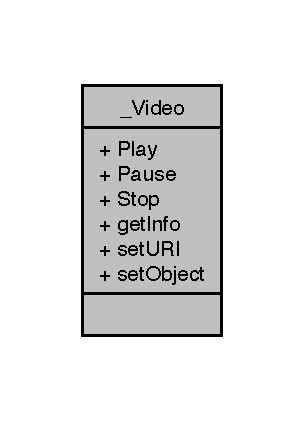
\includegraphics[width=146pt]{d5/da5/struct__Video__coll__graph}
\end{center}
\end{figure}
\subsection*{Data Fields}
\begin{DoxyCompactItemize}
\item 
\hypertarget{struct__Video_aef888a8e657f38d44001a2545ad9bcb1}{bool($\ast$ {\bfseries Play} )(\hyperlink{struct__Video}{Video} this\-\_\-gen)}\label{struct__Video_aef888a8e657f38d44001a2545ad9bcb1}

\item 
\hypertarget{struct__Video_a1144f0da810f7d94cf57acd612731803}{bool($\ast$ {\bfseries Pause} )(\hyperlink{struct__Video}{Video} this\-\_\-gen)}\label{struct__Video_a1144f0da810f7d94cf57acd612731803}

\item 
\hypertarget{struct__Video_a1c9916d4c5b3271d563d4857dc365a18}{bool($\ast$ {\bfseries Stop} )(\hyperlink{struct__Video}{Video} this\-\_\-gen)}\label{struct__Video_a1c9916d4c5b3271d563d4857dc365a18}

\item 
\hypertarget{struct__Video_a28466d9896b523beacac4a1add633aa6}{String($\ast$ {\bfseries get\-Info} )(\hyperlink{struct__Video}{Video} this\-\_\-gen, metadata\-\_\-extractor\-\_\-attr\-\_\-e element)}\label{struct__Video_a28466d9896b523beacac4a1add633aa6}

\item 
\hypertarget{struct__Video_a3d9407567e93bffc6b9121c742fa90e1}{bool($\ast$ {\bfseries set\-U\-R\-I} )(\hyperlink{struct__Video}{Video} this\-\_\-gen, String uri)}\label{struct__Video_a3d9407567e93bffc6b9121c742fa90e1}

\item 
\hypertarget{struct__Video_a42ce7237758001acc69e762904354aae}{bool($\ast$ {\bfseries set\-Object} )(\hyperlink{struct__Video}{Video} this\-\_\-gen, Evas\-\_\-\-Object $\ast$Evas\-Object)}\label{struct__Video_a42ce7237758001acc69e762904354aae}

\end{DoxyCompactItemize}


\subsection{Detailed Description}
Video 모듈에 대한 구조체이다. Video 모듈은 다양한 방식으로 동영상 파일을 제어 할 수 있다. 

\begin{DoxyNote}{Note}
File의 Video 모듈에 대한 구조체이다. \par
 구조체를 사용하기 전에 \hyperlink{File_8h_acc20c940b38ba0ace77f77a2992dea58}{New\-Video()} 함수를 사용해야 하며 사용이 끝났을 때 \hyperlink{File_8h_a23fb13c9330e924604c6d93e67e957c6}{Destroy\-Video()} 함수를 꼭 사용해야 한다. 
\end{DoxyNote}
\begin{DoxySeeAlso}{See Also}
\href{https://developer.tizen.org/dev-guide/2.3.0/org.tizen.native.mobile.apireference/group__CAPI__MEDIA__CONTENT__MODULE.html}{\tt https\-://developer.\-tizen.\-org/dev-\/guide/2.\-3.\-0/org.\-tizen.\-native.\-mobile.\-apireference/group\-\_\-\-\_\-\-C\-A\-P\-I\-\_\-\-\_\-\-M\-E\-D\-I\-A\-\_\-\-\_\-\-C\-O\-N\-T\-E\-N\-T\-\_\-\-\_\-\-M\-O\-D\-U\-L\-E.\-html} 
\end{DoxySeeAlso}


Definition at line 183 of file File.\-h.



The documentation for this struct was generated from the following file\-:\begin{DoxyCompactItemize}
\item 
\hyperlink{File_8h}{File.\-h}\end{DoxyCompactItemize}

\chapter{File Documentation}
\section{Bluetooth.\-c File Reference}
\label{Bluetooth_8c}\index{Bluetooth.\-c@{Bluetooth.\-c}}


Bluetooth A\-P\-I가 정의되어있다.  


{\ttfamily \#include \char`\"{}Commnucation/\-Bluetooth.\-h\char`\"{}}\\*
{\ttfamily \#include $<$stdlib.\-h$>$}\\*
{\ttfamily \#include $<$stdbool.\-h$>$}\\*
{\ttfamily \#include $<$system\-\_\-info.\-h$>$}\\*
{\ttfamily \#include $<$app\-\_\-control.\-h$>$}\\*
{\ttfamily \#include $<$dlog.\-h$>$}\\*
{\ttfamily \#include $<$glib.\-h$>$}\\*
Include dependency graph for Bluetooth.\-c\-:\nopagebreak
\begin{figure}[H]
\begin{center}
\leavevmode
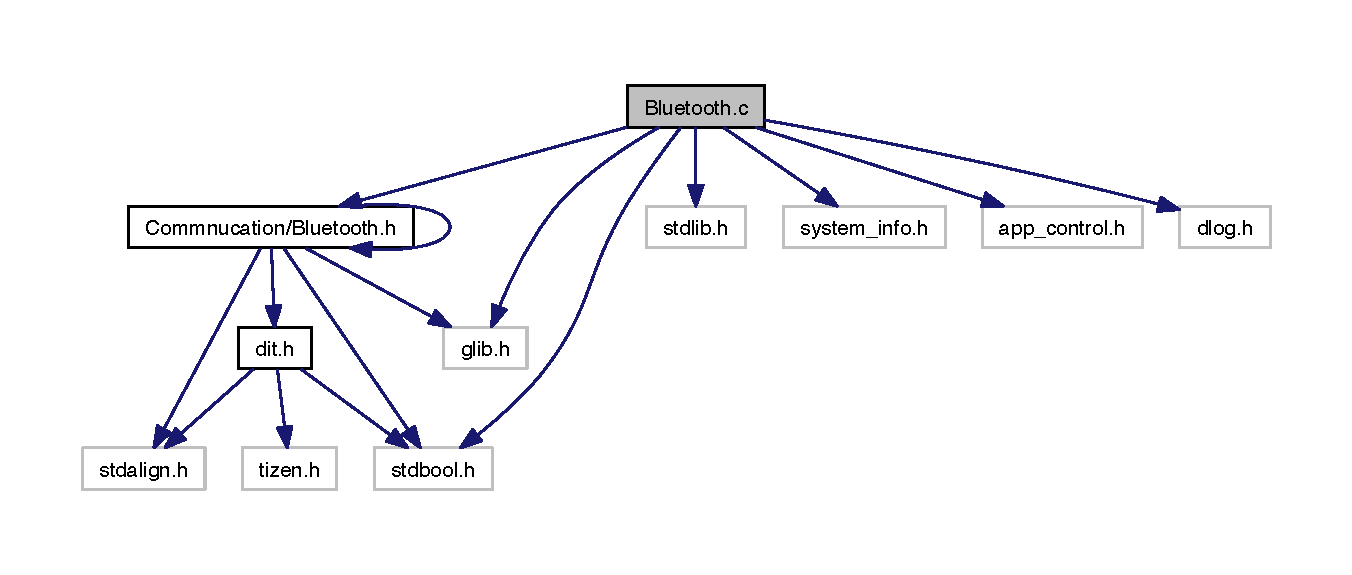
\includegraphics[width=350pt]{Bluetooth_8c__incl}
\end{center}
\end{figure}
\subsection*{Functions}
\begin{DoxyCompactItemize}
\item 
Bluetooth {\bf New\-Bluetooth} (void)
\begin{DoxyCompactList}\small\item\em 새로운 Bluetooth 객체를 생성한다. \end{DoxyCompactList}\item 
void {\bf Destroy\-Bluetooth} (Bluetooth this\-\_\-gen)
\begin{DoxyCompactList}\small\item\em 생성한 Bluetooth 객체를 소멸 시킨다. \end{DoxyCompactList}\item 
bool {\bf is\-Bluetooth\-Accessible} (Bluetooth this\-\_\-gen)
\begin{DoxyCompactList}\small\item\em 현재 Bluetooth 기능 지원 여부를 반환 한다. \end{DoxyCompactList}\item 
bool {\bf on\-Bluetooth\-Connect} (Bluetooth this\-\_\-gen)
\begin{DoxyCompactList}\small\item\em Bluetooth기기로 연결을 시도하며 이의 성공 여부를 반환한다. \end{DoxyCompactList}\item 
bool {\bf is\-Bluetooth\-Connected} (Bluetooth this\-\_\-gen)
\begin{DoxyCompactList}\small\item\em Bluetooth기기와의 연결 상태를 확인한다. \end{DoxyCompactList}\item 
bool {\bf on\-Bluetooth\-Disconnect} (Bluetooth this\-\_\-gen)
\begin{DoxyCompactList}\small\item\em Bluetooth기기로 연결을 해제하며 이의 성공 여부를 반환한다. \end{DoxyCompactList}\item 
bool {\bf Bluetooth\-File\-Recv} (Bluetooth this\-\_\-gen, String $\ast$recv\-Buffer)
\begin{DoxyCompactList}\small\item\em Bluetooth기기로 부터 데이터를 수신한다. \end{DoxyCompactList}\item 
bool {\bf Bluetooth\-File\-Send} (Bluetooth this\-\_\-gen, String sendbuffer)
\begin{DoxyCompactList}\small\item\em Bluetooth기기로 데이터를 송신한다. \end{DoxyCompactList}\item 
const char $\ast$ {\bf Bluetooth\-Error\-Check} (int err\-Code)
\begin{DoxyCompactList}\small\item\em Bluetooth A\-P\-I에서 발생하는 Error Code들을 확인 해준다. \end{DoxyCompactList}\end{DoxyCompactItemize}


\subsection{Detailed Description}
Bluetooth A\-P\-I가 정의되어있다. \begin{DoxyNote}{Note}
Bluetooth A\-P\-I가 정의되어있다. 
\end{DoxyNote}
\begin{DoxySeeAlso}{See Also}
\doxyref{Bluetooth.\-h}{p.}{Bluetooth_8h} 
\end{DoxySeeAlso}


\subsection{Function Documentation}
\index{Bluetooth.\-c@{Bluetooth.\-c}!Bluetooth\-Error\-Check@{Bluetooth\-Error\-Check}}
\index{Bluetooth\-Error\-Check@{Bluetooth\-Error\-Check}!Bluetooth.c@{Bluetooth.\-c}}
\subsubsection[{Bluetooth\-Error\-Check}]{\setlength{\rightskip}{0pt plus 5cm}const char$\ast$ Bluetooth\-Error\-Check (
\begin{DoxyParamCaption}
\item[{int}]{err\-Code}
\end{DoxyParamCaption}
)}\label{Bluetooth_8c_a27d2daee8cbfd1a01955b71a879af863}


Bluetooth A\-P\-I에서 발생하는 Error Code들을 확인 해준다. 


\begin{DoxyParams}[1]{Parameters}
\mbox{\tt in}  & {\em err\-Code} & 확인 하고자 하는 Error Code \\
\hline
\mbox{\tt out}  & {\em null} & \\
\hline
\end{DoxyParams}

\begin{DoxyRetVals}{Return values}
{\em B\-T\-\_\-\-E\-R\-R\-O\-R\-\_\-\-N\-O\-N\-E} & \-: Successful \\
\hline
{\em B\-T\-\_\-\-E\-R\-R\-O\-R\-\_\-\-C\-A\-N\-C\-E\-L\-L\-E\-D} & \-: Operation cancelled \\
\hline
{\em B\-T\-\_\-\-E\-R\-R\-O\-R\-\_\-\-I\-N\-V\-A\-L\-I\-D\-\_\-\-P\-A\-R\-A\-M\-E\-T\-E\-R} & \-: Invalid parameter \\
\hline
{\em B\-T\-\_\-\-E\-R\-R\-O\-R\-\_\-\-O\-U\-T\-\_\-\-O\-F\-\_\-\-M\-E\-M\-O\-R\-Y} & \-: Out of memory \\
\hline
{\em B\-T\-\_\-\-E\-R\-R\-O\-R\-\_\-\-R\-E\-S\-O\-U\-R\-C\-E\-\_\-\-B\-U\-S\-Y} & \-: Device or resource busy \\
\hline
{\em B\-T\-\_\-\-E\-R\-R\-O\-R\-\_\-\-T\-I\-M\-E\-D\-\_\-\-O\-U\-T} & \-: Timeout error \\
\hline
{\em B\-T\-\_\-\-E\-R\-R\-O\-R\-\_\-\-N\-O\-W\-\_\-\-I\-N\-\_\-\-P\-R\-O\-G\-R\-E\-S\-S} & \-: Operation now in progress \\
\hline
{\em B\-T\-\_\-\-E\-R\-R\-O\-R\-\_\-\-N\-O\-T\-\_\-\-S\-U\-P\-P\-O\-R\-T\-E\-D} & \-: Not Supported \\
\hline
{\em B\-T\-\_\-\-E\-R\-R\-O\-R\-\_\-\-P\-E\-R\-M\-I\-S\-S\-I\-O\-N\-\_\-\-D\-E\-N\-I\-E\-D} & \-: Permission denied \\
\hline
{\em B\-T\-\_\-\-E\-R\-R\-O\-R\-\_\-\-Q\-U\-O\-T\-A\-\_\-\-E\-X\-C\-E\-E\-D\-E\-D} & \-: Quota exceeded \\
\hline
{\em B\-T\-\_\-\-E\-R\-R\-O\-R\-\_\-\-N\-O\-T\-\_\-\-I\-N\-I\-T\-I\-A\-L\-I\-Z\-E\-D} & \-: Local adapter not initialized \\
\hline
{\em B\-T\-\_\-\-E\-R\-R\-O\-R\-\_\-\-N\-O\-T\-\_\-\-E\-N\-A\-B\-L\-E\-D} & \-: Local adapter not enabled \\
\hline
{\em B\-T\-\_\-\-E\-R\-R\-O\-R\-\_\-\-A\-L\-R\-E\-A\-D\-Y\-\_\-\-D\-O\-N\-E} & \-: Operation already done \\
\hline
{\em B\-T\-\_\-\-E\-R\-R\-O\-R\-\_\-\-O\-P\-E\-R\-A\-T\-I\-O\-N\-\_\-\-F\-A\-I\-L\-E\-D} & \-: Operation failed \\
\hline
{\em B\-T\-\_\-\-E\-R\-R\-O\-R\-\_\-\-N\-O\-T\-\_\-\-I\-N\-\_\-\-P\-R\-O\-G\-R\-E\-S\-S} & \-: Operation not in progress \\
\hline
{\em B\-T\-\_\-\-E\-R\-R\-O\-R\-\_\-\-R\-E\-M\-O\-T\-E\-\_\-\-D\-E\-V\-I\-C\-E\-\_\-\-N\-O\-T\-\_\-\-B\-O\-N\-D\-E\-D} & \-: Remote device not bonded \\
\hline
{\em B\-T\-\_\-\-E\-R\-R\-O\-R\-\_\-\-A\-U\-T\-H\-\_\-\-R\-E\-J\-E\-C\-T\-E\-D} & \-: Authentication rejected \\
\hline
{\em B\-T\-\_\-\-E\-R\-R\-O\-R\-\_\-\-A\-U\-T\-H\-\_\-\-F\-A\-I\-L\-E\-D} & \-: Authentication failed \\
\hline
{\em B\-T\-\_\-\-E\-R\-R\-O\-R\-\_\-\-R\-E\-M\-O\-T\-E\-\_\-\-D\-E\-V\-I\-C\-E\-\_\-\-N\-O\-T\-\_\-\-F\-O\-U\-N\-D} & \-: Remote device not found \\
\hline
{\em B\-T\-\_\-\-E\-R\-R\-O\-R\-\_\-\-S\-E\-R\-V\-I\-C\-E\-\_\-\-S\-E\-A\-R\-C\-H\-\_\-\-F\-A\-I\-L\-E\-D} & \-: Service search failed \\
\hline
{\em B\-T\-\_\-\-E\-R\-R\-O\-R\-\_\-\-R\-E\-M\-O\-T\-E\-\_\-\-D\-E\-V\-I\-C\-E\-\_\-\-N\-O\-T\-\_\-\-C\-O\-N\-N\-E\-C\-T\-E\-D} & \-: Remote device is not connected \\
\hline
{\em B\-T\-\_\-\-E\-R\-R\-O\-R\-\_\-\-A\-G\-A\-I\-N} & \-: Resource temporarily unavailable \\
\hline
{\em B\-T\-\_\-\-E\-R\-R\-O\-R\-\_\-\-S\-E\-R\-V\-I\-C\-E\-\_\-\-N\-O\-T\-\_\-\-F\-O\-U\-N\-D} & \-: Service Not Found \\
\hline
{\em B\-T\-\_\-\-E\-R\-R\-O\-R\-\_\-\-U\-N\-K\-N\-W\-O\-N} & \-: Unknown error occurred \\
\hline
\end{DoxyRetVals}
\begin{DoxyNote}{Note}
Bluetooth A\-P\-I에서 발생하는 Error Code들을 확인 해준다. \par
 Error의 내용은 Log를 통해 출력 된다. \par
 24가지의 Error Code들을 확인 가능 하다. 
\end{DoxyNote}
\begin{DoxySeeAlso}{See Also}
{\tt Tizen Native A\-P\-I Document -\/ Bluetooth part} 
\end{DoxySeeAlso}


Here is the caller graph for this function\-:\nopagebreak
\begin{figure}[H]
\begin{center}
\leavevmode
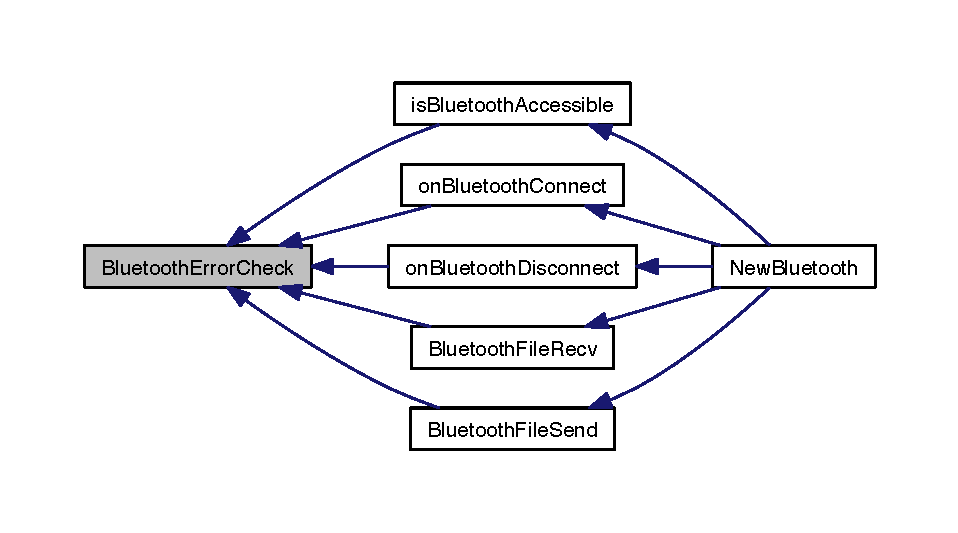
\includegraphics[width=350pt]{Bluetooth_8c_a27d2daee8cbfd1a01955b71a879af863_icgraph}
\end{center}
\end{figure}


\index{Bluetooth.\-c@{Bluetooth.\-c}!Bluetooth\-File\-Recv@{Bluetooth\-File\-Recv}}
\index{Bluetooth\-File\-Recv@{Bluetooth\-File\-Recv}!Bluetooth.c@{Bluetooth.\-c}}
\subsubsection[{Bluetooth\-File\-Recv}]{\setlength{\rightskip}{0pt plus 5cm}bool Bluetooth\-File\-Recv (
\begin{DoxyParamCaption}
\item[{Bluetooth}]{this\-\_\-gen, }
\item[{String $\ast$}]{recv\-Buffer}
\end{DoxyParamCaption}
)}\label{Bluetooth_8c_a43d4d767fbb4f0a1568a453e7b6a9995}


Bluetooth기기로 부터 데이터를 수신한다. 


\begin{DoxyParams}[1]{Parameters}
\mbox{\tt in}  & {\em this\-\_\-gen} & 데이터를 수신할 Bluetooth 객체 \\
\hline
\mbox{\tt in}  & {\em recv\-Buffer} & 수신할 데이터 주소 \\
\hline
\mbox{\tt out}  & {\em recv\-Buffer} & 수신한 데이터 \\
\hline
\end{DoxyParams}

\begin{DoxyRetVals}{Return values}
{\em bool} & \par
 함수의 성공 여부를 반환한다. \par
 실패시 {\ttfamily false를} 반환하며 상세한 원인을 Log로 출력한다. \\
\hline
\end{DoxyRetVals}
\begin{DoxyNote}{Note}
Bluetooth기기로 부터 데이터를 수신한다. 
\end{DoxyNote}
\begin{DoxySeeAlso}{See Also}
\doxyref{New\-Bluetooth}{p.}{Bluetooth_8h_aedecb2f1b25b6d408a1880978b66712a} \par
 \doxyref{Destroy\-Bluetooth}{p.}{Bluetooth_8h_a643b6a392ddbcf1c02bcfeb15ca52df8} \par
 \doxyref{is\-Bluetooth\-Accessible}{p.}{Bluetooth_8h_a00b401ae906bf1d77f232c88a14314fc} \par
 \doxyref{on\-Bluetooth\-Connect}{p.}{Bluetooth_8h_a77d0c6bf9a2f45a43a3b5801dd978fb6} \par
 \doxyref{is\-Bluetooth\-Connected}{p.}{Bluetooth_8h_a4959b3be5e12c0d3e4cc317e00e4621e} \par
 \doxyref{on\-Bluetooth\-Disconnect}{p.}{Bluetooth_8h_a26f809a19ded06421baab533eb8a59a6} \par
 \doxyref{Bluetooth\-File\-Send}{p.}{Bluetooth_8h_a169790dd12357103f392285063a4cfb9} 
\end{DoxySeeAlso}
\begin{DoxyPrecond}{Precondition}
{\bfseries feature} \par

\begin{DoxyItemize}
\item {\tt http\-://tizen.\-org/feature/network.\-bluetooth} 
\end{DoxyItemize}
\end{DoxyPrecond}


Here is the call graph for this function\-:\nopagebreak
\begin{figure}[H]
\begin{center}
\leavevmode
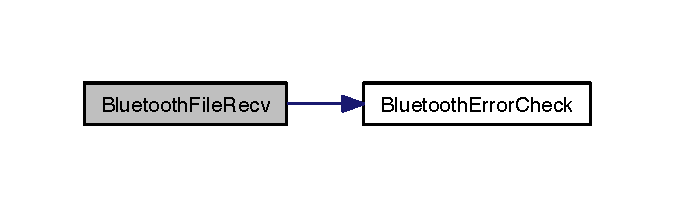
\includegraphics[width=324pt]{Bluetooth_8c_a43d4d767fbb4f0a1568a453e7b6a9995_cgraph}
\end{center}
\end{figure}




Here is the caller graph for this function\-:\nopagebreak
\begin{figure}[H]
\begin{center}
\leavevmode
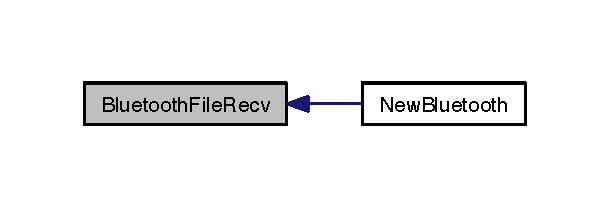
\includegraphics[width=292pt]{Bluetooth_8c_a43d4d767fbb4f0a1568a453e7b6a9995_icgraph}
\end{center}
\end{figure}


\index{Bluetooth.\-c@{Bluetooth.\-c}!Bluetooth\-File\-Send@{Bluetooth\-File\-Send}}
\index{Bluetooth\-File\-Send@{Bluetooth\-File\-Send}!Bluetooth.c@{Bluetooth.\-c}}
\subsubsection[{Bluetooth\-File\-Send}]{\setlength{\rightskip}{0pt plus 5cm}bool Bluetooth\-File\-Send (
\begin{DoxyParamCaption}
\item[{Bluetooth}]{this\-\_\-gen, }
\item[{String}]{sendbuffer}
\end{DoxyParamCaption}
)}\label{Bluetooth_8c_a169790dd12357103f392285063a4cfb9}


Bluetooth기기로 데이터를 송신한다. 


\begin{DoxyParams}[1]{Parameters}
\mbox{\tt in}  & {\em this\-\_\-gen} & 데이터를 송신할 Bluetooth 객체 \\
\hline
\mbox{\tt in}  & {\em sendbuffer} & 송신할 파일 path \\
\hline
\mbox{\tt out}  & {\em null} & \\
\hline
\end{DoxyParams}

\begin{DoxyRetVals}{Return values}
{\em bool} & \par
 함수의 성공 여부를 반환한다. \par
 실패시 {\ttfamily false를} 반환하며 상세한 원인을 Log로 출력한다. \\
\hline
\end{DoxyRetVals}
\begin{DoxyNote}{Note}
Bluetooth기기로 데이터를 송신한다. \par

\end{DoxyNote}
\begin{DoxySeeAlso}{See Also}
\doxyref{New\-Bluetooth}{p.}{Bluetooth_8h_aedecb2f1b25b6d408a1880978b66712a} \par
 \doxyref{Destroy\-Bluetooth}{p.}{Bluetooth_8h_a643b6a392ddbcf1c02bcfeb15ca52df8} \par
 \doxyref{is\-Bluetooth\-Accessible}{p.}{Bluetooth_8h_a00b401ae906bf1d77f232c88a14314fc} \par
 \doxyref{on\-Bluetooth\-Connect}{p.}{Bluetooth_8h_a77d0c6bf9a2f45a43a3b5801dd978fb6} \par
 \doxyref{is\-Bluetooth\-Connected}{p.}{Bluetooth_8h_a4959b3be5e12c0d3e4cc317e00e4621e} \par
 \doxyref{on\-Bluetooth\-Disconnect}{p.}{Bluetooth_8h_a26f809a19ded06421baab533eb8a59a6} \par
 \doxyref{Bluetooth\-File\-Recv}{p.}{Bluetooth_8h_a43d4d767fbb4f0a1568a453e7b6a9995} 
\end{DoxySeeAlso}
\begin{DoxyPrecond}{Precondition}
{\bfseries feature} \par

\begin{DoxyItemize}
\item {\tt http\-://tizen.\-org/feature/network.\-bluetooth} 
\end{DoxyItemize}
\end{DoxyPrecond}


Here is the call graph for this function\-:\nopagebreak
\begin{figure}[H]
\begin{center}
\leavevmode
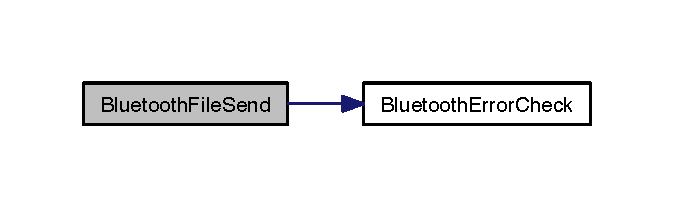
\includegraphics[width=324pt]{Bluetooth_8c_a169790dd12357103f392285063a4cfb9_cgraph}
\end{center}
\end{figure}




Here is the caller graph for this function\-:\nopagebreak
\begin{figure}[H]
\begin{center}
\leavevmode
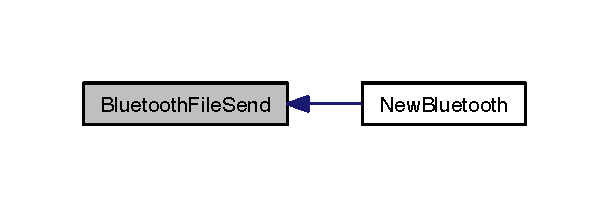
\includegraphics[width=292pt]{Bluetooth_8c_a169790dd12357103f392285063a4cfb9_icgraph}
\end{center}
\end{figure}


\index{Bluetooth.\-c@{Bluetooth.\-c}!Destroy\-Bluetooth@{Destroy\-Bluetooth}}
\index{Destroy\-Bluetooth@{Destroy\-Bluetooth}!Bluetooth.c@{Bluetooth.\-c}}
\subsubsection[{Destroy\-Bluetooth}]{\setlength{\rightskip}{0pt plus 5cm}void Destroy\-Bluetooth (
\begin{DoxyParamCaption}
\item[{Bluetooth}]{this\-\_\-gen}
\end{DoxyParamCaption}
)}\label{Bluetooth_8c_a643b6a392ddbcf1c02bcfeb15ca52df8}


생성한 Bluetooth 객체를 소멸 시킨다. 


\begin{DoxyParams}[1]{Parameters}
\mbox{\tt in}  & {\em this\-\_\-gen} & 소멸시킬 Bluetooth 객체 \\
\hline
\mbox{\tt out}  & {\em null} & \\
\hline
\end{DoxyParams}

\begin{DoxyRetVals}{Return values}
{\em void} & \\
\hline
\end{DoxyRetVals}
\begin{DoxyNote}{Note}
생성한 Bluetooth 객체를 소멸 시킨다. \par
 Bluetooth 객체를 사용한 후 반드시 호출해야 한다. 
\end{DoxyNote}
\begin{DoxySeeAlso}{See Also}
\doxyref{New\-Bluetooth}{p.}{Bluetooth_8h_aedecb2f1b25b6d408a1880978b66712a} 
\end{DoxySeeAlso}
\begin{DoxyPrecond}{Precondition}
{\bfseries feature} \par

\begin{DoxyItemize}
\item {\tt http\-://tizen.\-org/feature/network.\-bluetooth} 
\end{DoxyItemize}
\end{DoxyPrecond}
\index{Bluetooth.\-c@{Bluetooth.\-c}!is\-Bluetooth\-Accessible@{is\-Bluetooth\-Accessible}}
\index{is\-Bluetooth\-Accessible@{is\-Bluetooth\-Accessible}!Bluetooth.c@{Bluetooth.\-c}}
\subsubsection[{is\-Bluetooth\-Accessible}]{\setlength{\rightskip}{0pt plus 5cm}bool is\-Bluetooth\-Accessible (
\begin{DoxyParamCaption}
\item[{Bluetooth}]{this\-\_\-gen}
\end{DoxyParamCaption}
)}\label{Bluetooth_8c_a00b401ae906bf1d77f232c88a14314fc}


현재 Bluetooth 기능 지원 여부를 반환 한다. 


\begin{DoxyParams}[1]{Parameters}
\mbox{\tt in}  & {\em this\-\_\-gen} & 사용 가능 여부를 반환 할 Bluetooth 객체 \\
\hline
\mbox{\tt out}  & {\em null} & \\
\hline
\end{DoxyParams}

\begin{DoxyRetVals}{Return values}
{\em bool} & \par
 함수의 성공 여부를 반환한다. \par
 실패시 {\ttfamily false를} 반환하며 상세한 원인을 Log로 출력한다. \\
\hline
\end{DoxyRetVals}
\begin{DoxyNote}{Note}
현재 Bluetooth 기능 지원 여부를 반환 한다. \par
 지원 가능 이라면 {\ttfamily true}, 지원 가능이 아니라면 {\ttfamily false를} 반환한다. 
\end{DoxyNote}
\begin{DoxySeeAlso}{See Also}
\doxyref{New\-Bluetooth}{p.}{Bluetooth_8h_aedecb2f1b25b6d408a1880978b66712a} \par
 \doxyref{Destroy\-Bluetooth}{p.}{Bluetooth_8h_a643b6a392ddbcf1c02bcfeb15ca52df8} \par
 \doxyref{on\-Bluetooth\-Connect}{p.}{Bluetooth_8h_a77d0c6bf9a2f45a43a3b5801dd978fb6} \par
 \doxyref{is\-Bluetooth\-Connected}{p.}{Bluetooth_8h_a4959b3be5e12c0d3e4cc317e00e4621e} \par
 \doxyref{on\-Bluetooth\-Disconnect}{p.}{Bluetooth_8h_a26f809a19ded06421baab533eb8a59a6} \par
 \doxyref{Bluetooth\-File\-Send}{p.}{Bluetooth_8h_a169790dd12357103f392285063a4cfb9} \par
 \doxyref{Bluetooth\-File\-Recv}{p.}{Bluetooth_8h_a43d4d767fbb4f0a1568a453e7b6a9995} 
\end{DoxySeeAlso}
\begin{DoxyPrecond}{Precondition}
{\bfseries feature} \par

\begin{DoxyItemize}
\item {\tt http\-://tizen.\-org/feature/network.\-bluetooth} 
\end{DoxyItemize}
\end{DoxyPrecond}


Here is the call graph for this function\-:\nopagebreak
\begin{figure}[H]
\begin{center}
\leavevmode
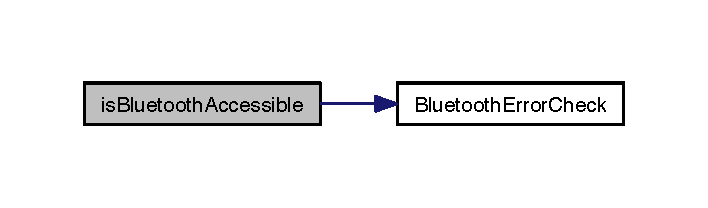
\includegraphics[width=340pt]{Bluetooth_8c_a00b401ae906bf1d77f232c88a14314fc_cgraph}
\end{center}
\end{figure}




Here is the caller graph for this function\-:\nopagebreak
\begin{figure}[H]
\begin{center}
\leavevmode
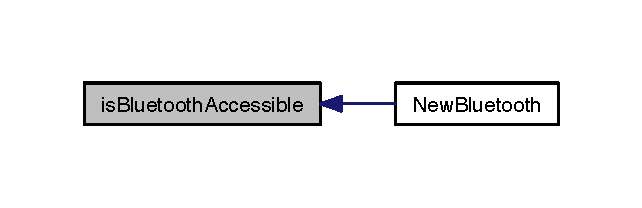
\includegraphics[width=308pt]{Bluetooth_8c_a00b401ae906bf1d77f232c88a14314fc_icgraph}
\end{center}
\end{figure}


\index{Bluetooth.\-c@{Bluetooth.\-c}!is\-Bluetooth\-Connected@{is\-Bluetooth\-Connected}}
\index{is\-Bluetooth\-Connected@{is\-Bluetooth\-Connected}!Bluetooth.c@{Bluetooth.\-c}}
\subsubsection[{is\-Bluetooth\-Connected}]{\setlength{\rightskip}{0pt plus 5cm}bool is\-Bluetooth\-Connected (
\begin{DoxyParamCaption}
\item[{Bluetooth}]{this\-\_\-gen}
\end{DoxyParamCaption}
)}\label{Bluetooth_8c_a4959b3be5e12c0d3e4cc317e00e4621e}


Bluetooth기기와의 연결 상태를 확인한다. 


\begin{DoxyParams}[1]{Parameters}
\mbox{\tt in}  & {\em this\-\_\-gen} & 연결 상태를 확인할 Bluetooth 객체 \\
\hline
\mbox{\tt out}  & {\em null} & \\
\hline
\end{DoxyParams}

\begin{DoxyRetVals}{Return values}
{\em bool} & \par
 함수의 성공 여부를 반환한다. \par
 실패시 {\ttfamily false를} 반환하며 상세한 원인을 Log로 출력한다. \\
\hline
\end{DoxyRetVals}
\begin{DoxyNote}{Note}
Bluetooth기기와의 연결 상태를 확인한다. \par
 연결되어 있다면 {\ttfamily true}, 연결되어 있지 않다면 {\ttfamily false를} 반환한다. 
\end{DoxyNote}
\begin{DoxySeeAlso}{See Also}
\doxyref{New\-Bluetooth}{p.}{Bluetooth_8h_aedecb2f1b25b6d408a1880978b66712a} \par
 \doxyref{Destroy\-Bluetooth}{p.}{Bluetooth_8h_a643b6a392ddbcf1c02bcfeb15ca52df8} \par
 \doxyref{is\-Bluetooth\-Accessible}{p.}{Bluetooth_8h_a00b401ae906bf1d77f232c88a14314fc} \par
 \doxyref{on\-Bluetooth\-Connect}{p.}{Bluetooth_8h_a77d0c6bf9a2f45a43a3b5801dd978fb6} \par
 \doxyref{on\-Bluetooth\-Disconnect}{p.}{Bluetooth_8h_a26f809a19ded06421baab533eb8a59a6} \par
 \doxyref{Bluetooth\-File\-Send}{p.}{Bluetooth_8h_a169790dd12357103f392285063a4cfb9} \par
 \doxyref{Bluetooth\-File\-Recv}{p.}{Bluetooth_8h_a43d4d767fbb4f0a1568a453e7b6a9995} 
\end{DoxySeeAlso}
\begin{DoxyPrecond}{Precondition}
{\bfseries feature} \par

\begin{DoxyItemize}
\item {\tt http\-://tizen.\-org/feature/network.\-bluetooth} 
\end{DoxyItemize}
\end{DoxyPrecond}


Here is the caller graph for this function\-:\nopagebreak
\begin{figure}[H]
\begin{center}
\leavevmode
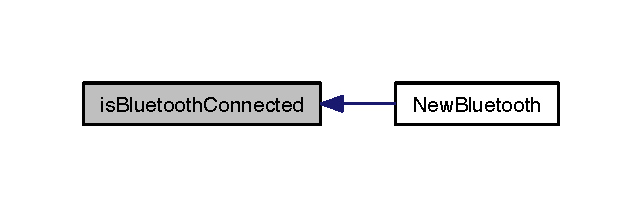
\includegraphics[width=308pt]{Bluetooth_8c_a4959b3be5e12c0d3e4cc317e00e4621e_icgraph}
\end{center}
\end{figure}


\index{Bluetooth.\-c@{Bluetooth.\-c}!New\-Bluetooth@{New\-Bluetooth}}
\index{New\-Bluetooth@{New\-Bluetooth}!Bluetooth.c@{Bluetooth.\-c}}
\subsubsection[{New\-Bluetooth}]{\setlength{\rightskip}{0pt plus 5cm}Bluetooth New\-Bluetooth (
\begin{DoxyParamCaption}
\item[{void}]{}
\end{DoxyParamCaption}
)}\label{Bluetooth_8c_aedecb2f1b25b6d408a1880978b66712a}


새로운 Bluetooth 객체를 생성한다. 


\begin{DoxyParams}[1]{Parameters}
\mbox{\tt in}  & {\em void} & \\
\hline
\mbox{\tt out}  & {\em null} & \\
\hline
\end{DoxyParams}

\begin{DoxyRetVals}{Return values}
{\em Bluetooth} & \\
\hline
\end{DoxyRetVals}
\begin{DoxyNote}{Note}
새로운 Bluetooth 객체를 생성한다. \par
 Bluetooth 객체를 사용하기 전에 반드시 호출해야 한다. 
\end{DoxyNote}
\begin{DoxySeeAlso}{See Also}
\doxyref{Destroy\-Bluetooth}{p.}{Bluetooth_8h_a643b6a392ddbcf1c02bcfeb15ca52df8} \par
 \doxyref{is\-Bluetooth\-Accessible}{p.}{Bluetooth_8h_a00b401ae906bf1d77f232c88a14314fc} \par
 \doxyref{on\-Bluetooth\-Connect}{p.}{Bluetooth_8h_a77d0c6bf9a2f45a43a3b5801dd978fb6} \par
 \doxyref{is\-Bluetooth\-Connected}{p.}{Bluetooth_8h_a4959b3be5e12c0d3e4cc317e00e4621e} \par
 \doxyref{on\-Bluetooth\-Disconnect}{p.}{Bluetooth_8h_a26f809a19ded06421baab533eb8a59a6} \par
 \doxyref{Bluetooth\-File\-Send}{p.}{Bluetooth_8h_a169790dd12357103f392285063a4cfb9} \par
 \doxyref{Bluetooth\-File\-Recv}{p.}{Bluetooth_8h_a43d4d767fbb4f0a1568a453e7b6a9995} 
\end{DoxySeeAlso}
\begin{DoxyPrecond}{Precondition}
{\bfseries feature} \par

\begin{DoxyItemize}
\item {\tt http\-://tizen.\-org/feature/network.\-bluetooth} 
\end{DoxyItemize}
\end{DoxyPrecond}
\begin{DoxyWarning}{Warning}
사용이 끝났을 때 \doxyref{Destroy\-Bluetooth()}{p.}{Bluetooth_8h_a643b6a392ddbcf1c02bcfeb15ca52df8} 함수를 꼭 사용해야 한다.
\end{DoxyWarning}

\begin{DoxyCode}
Bluetooth NewBluetooth (\textcolor{keywordtype}{void})
\{
    BluetoothExtends * \textcolor{keyword}{this} = malloc (\textcolor{keyword}{sizeof} (BluetoothExtends));
    this->bluetooth.isAccessible = isBluetoothAccessible;
    this->bluetooth.onConnect    = onBluetoothConnect;
    this->bluetooth.isConnected  = isBluetoothConnected;
    this->bluetooth.onDisconnect = onBluetoothDisconnect;
    this->bluetooth.FileRecv     = BluetoothFileRecv;
    this->bluetooth.FileSend     = BluetoothFileSend;

    this->connected     = \textcolor{keyword}{false};
    this->accessible    = \textcolor{keyword}{false};
    this->remoteMACAddr = NULL;

    \textcolor{keywordflow}{return} &this->bluetooth;
\}
\end{DoxyCode}
 

Here is the call graph for this function\-:\nopagebreak
\begin{figure}[H]
\begin{center}
\leavevmode
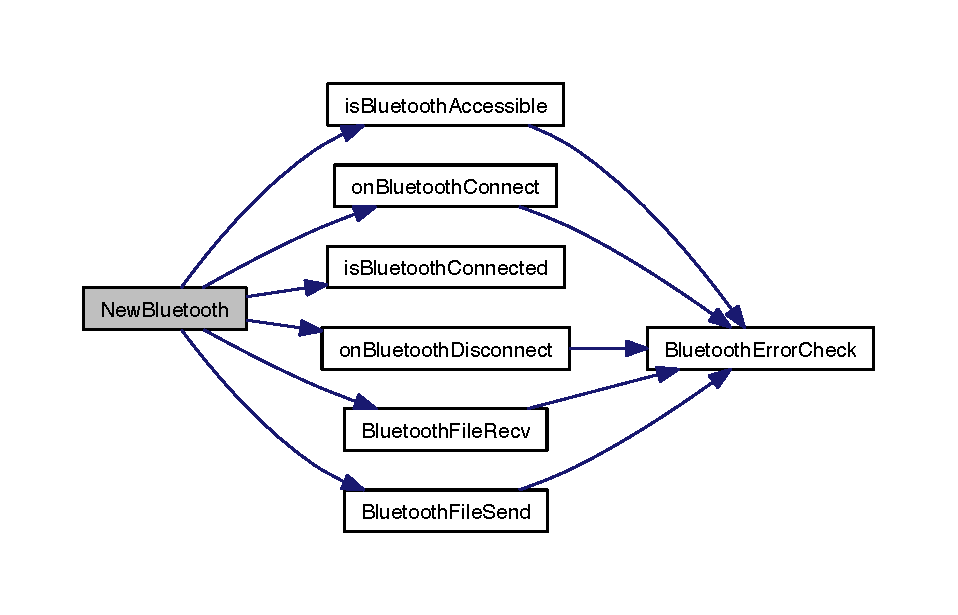
\includegraphics[width=350pt]{Bluetooth_8c_aedecb2f1b25b6d408a1880978b66712a_cgraph}
\end{center}
\end{figure}


\index{Bluetooth.\-c@{Bluetooth.\-c}!on\-Bluetooth\-Connect@{on\-Bluetooth\-Connect}}
\index{on\-Bluetooth\-Connect@{on\-Bluetooth\-Connect}!Bluetooth.c@{Bluetooth.\-c}}
\subsubsection[{on\-Bluetooth\-Connect}]{\setlength{\rightskip}{0pt plus 5cm}bool on\-Bluetooth\-Connect (
\begin{DoxyParamCaption}
\item[{Bluetooth}]{this\-\_\-gen}
\end{DoxyParamCaption}
)}\label{Bluetooth_8c_a77d0c6bf9a2f45a43a3b5801dd978fb6}


Bluetooth기기로 연결을 시도하며 이의 성공 여부를 반환한다. 


\begin{DoxyParams}[1]{Parameters}
\mbox{\tt in}  & {\em this\-\_\-gen} & 연결 성공 여부를 확인할 Bluetooth 객체 \\
\hline
\mbox{\tt out}  & {\em null} & \\
\hline
\end{DoxyParams}

\begin{DoxyRetVals}{Return values}
{\em bool} & \par
 함수의 성공 여부를 반환한다. \par
 실패시 {\ttfamily false를} 반환하며 상세한 원인을 Log로 출력한다. \\
\hline
\end{DoxyRetVals}
\begin{DoxyNote}{Note}
Bluetooth기기로 연결을 시도하며 이의 성공 여부를 반환한다. \par
 연결에 성공하면 {\ttfamily true}, 실패하면 {\ttfamily false를} 반환한다. 
\end{DoxyNote}
\begin{DoxySeeAlso}{See Also}
\doxyref{New\-Bluetooth}{p.}{Bluetooth_8h_aedecb2f1b25b6d408a1880978b66712a} \par
 \doxyref{Destroy\-Bluetooth}{p.}{Bluetooth_8h_a643b6a392ddbcf1c02bcfeb15ca52df8} \par
 \doxyref{is\-Bluetooth\-Accessible}{p.}{Bluetooth_8h_a00b401ae906bf1d77f232c88a14314fc} \par
 \doxyref{is\-Bluetooth\-Connected}{p.}{Bluetooth_8h_a4959b3be5e12c0d3e4cc317e00e4621e} \par
 \doxyref{on\-Bluetooth\-Disconnect}{p.}{Bluetooth_8h_a26f809a19ded06421baab533eb8a59a6} \par
 \doxyref{Bluetooth\-File\-Send}{p.}{Bluetooth_8h_a169790dd12357103f392285063a4cfb9} \par
 \doxyref{Bluetooth\-File\-Recv}{p.}{Bluetooth_8h_a43d4d767fbb4f0a1568a453e7b6a9995} 
\end{DoxySeeAlso}
\begin{DoxyPrecond}{Precondition}
{\bfseries feature} \par

\begin{DoxyItemize}
\item {\tt http\-://tizen.\-org/feature/network.\-bluetooth} 
\end{DoxyItemize}
\end{DoxyPrecond}


Here is the call graph for this function\-:\nopagebreak
\begin{figure}[H]
\begin{center}
\leavevmode
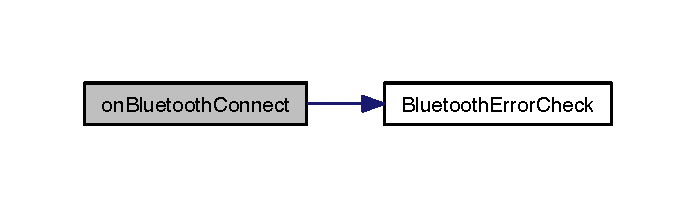
\includegraphics[width=334pt]{Bluetooth_8c_a77d0c6bf9a2f45a43a3b5801dd978fb6_cgraph}
\end{center}
\end{figure}




Here is the caller graph for this function\-:\nopagebreak
\begin{figure}[H]
\begin{center}
\leavevmode
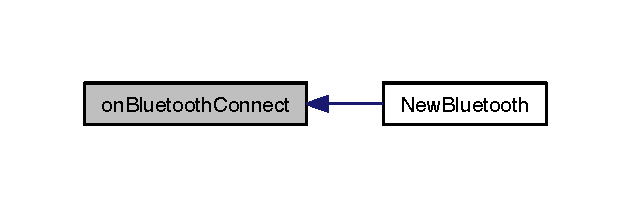
\includegraphics[width=302pt]{Bluetooth_8c_a77d0c6bf9a2f45a43a3b5801dd978fb6_icgraph}
\end{center}
\end{figure}


\index{Bluetooth.\-c@{Bluetooth.\-c}!on\-Bluetooth\-Disconnect@{on\-Bluetooth\-Disconnect}}
\index{on\-Bluetooth\-Disconnect@{on\-Bluetooth\-Disconnect}!Bluetooth.c@{Bluetooth.\-c}}
\subsubsection[{on\-Bluetooth\-Disconnect}]{\setlength{\rightskip}{0pt plus 5cm}bool on\-Bluetooth\-Disconnect (
\begin{DoxyParamCaption}
\item[{Bluetooth}]{this\-\_\-gen}
\end{DoxyParamCaption}
)}\label{Bluetooth_8c_a26f809a19ded06421baab533eb8a59a6}


Bluetooth기기로 연결을 해제하며 이의 성공 여부를 반환한다. 


\begin{DoxyParams}[1]{Parameters}
\mbox{\tt in}  & {\em this\-\_\-gen} & 연결 해제 여부를 확인할 Bluetooth 객체 \\
\hline
\mbox{\tt out}  & {\em null} & \\
\hline
\end{DoxyParams}

\begin{DoxyRetVals}{Return values}
{\em bool} & \par
 함수의 성공 여부를 반환한다. \par
 실패시 {\ttfamily false를} 반환하며 상세한 원인을 Log로 출력한다. \\
\hline
\end{DoxyRetVals}
\begin{DoxyNote}{Note}
Bluetooth기기로 연결을 해제하며 이의 성공 여부를 반환한다. \par
 연결 해제에 성공하면 {\ttfamily true}, 실패하면 {\ttfamily false를} 반환한다. 
\end{DoxyNote}
\begin{DoxySeeAlso}{See Also}
\doxyref{New\-Bluetooth}{p.}{Bluetooth_8h_aedecb2f1b25b6d408a1880978b66712a} \par
 \doxyref{Destroy\-Bluetooth}{p.}{Bluetooth_8h_a643b6a392ddbcf1c02bcfeb15ca52df8} \par
 \doxyref{is\-Bluetooth\-Accessible}{p.}{Bluetooth_8h_a00b401ae906bf1d77f232c88a14314fc} \par
 \doxyref{on\-Bluetooth\-Connect}{p.}{Bluetooth_8h_a77d0c6bf9a2f45a43a3b5801dd978fb6} \par
 \doxyref{is\-Bluetooth\-Connected}{p.}{Bluetooth_8h_a4959b3be5e12c0d3e4cc317e00e4621e} \par
 \doxyref{Bluetooth\-File\-Send}{p.}{Bluetooth_8h_a169790dd12357103f392285063a4cfb9} \par
 \doxyref{Bluetooth\-File\-Recv}{p.}{Bluetooth_8h_a43d4d767fbb4f0a1568a453e7b6a9995} 
\end{DoxySeeAlso}
\begin{DoxyPrecond}{Precondition}
{\bfseries feature} \par

\begin{DoxyItemize}
\item {\tt http\-://tizen.\-org/feature/network.\-bluetooth} 
\end{DoxyItemize}
\end{DoxyPrecond}


Here is the call graph for this function\-:\nopagebreak
\begin{figure}[H]
\begin{center}
\leavevmode
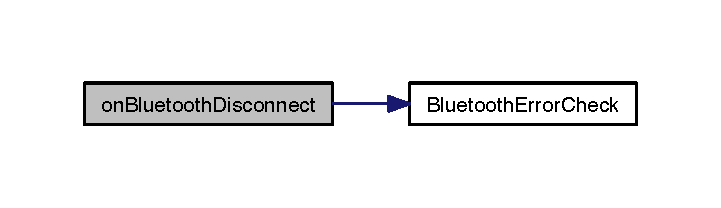
\includegraphics[width=346pt]{Bluetooth_8c_a26f809a19ded06421baab533eb8a59a6_cgraph}
\end{center}
\end{figure}




Here is the caller graph for this function\-:\nopagebreak
\begin{figure}[H]
\begin{center}
\leavevmode
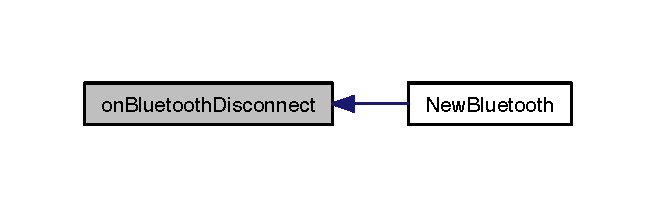
\includegraphics[width=314pt]{Bluetooth_8c_a26f809a19ded06421baab533eb8a59a6_icgraph}
\end{center}
\end{figure}



\section{Bluetooth.\-h File Reference}
\label{Bluetooth_8h}\index{Bluetooth.\-h@{Bluetooth.\-h}}


Bluetooth A\-P\-I 를 사용하기 위해 포함해야 하는 헤더이다.  


{\ttfamily \#include $<$stdbool.\-h$>$}\\*
{\ttfamily \#include $<$stdalign.\-h$>$}\\*
{\ttfamily \#include \char`\"{}dit.\-h\char`\"{}}\\*
{\ttfamily \#include $<$glib.\-h$>$}\\*
{\ttfamily \#include $<$bluetooth.\-h$>$}\\*
Include dependency graph for Bluetooth.\-h\-:
\nopagebreak
\begin{figure}[H]
\begin{center}
\leavevmode
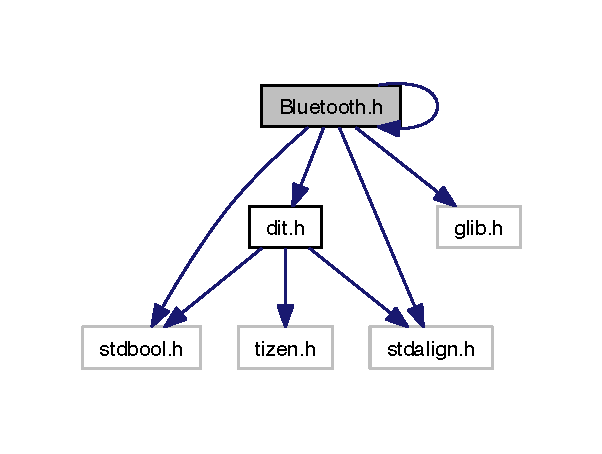
\includegraphics[width=289pt]{Bluetooth_8h__incl}
\end{center}
\end{figure}
This graph shows which files directly or indirectly include this file\-:
\nopagebreak
\begin{figure}[H]
\begin{center}
\leavevmode
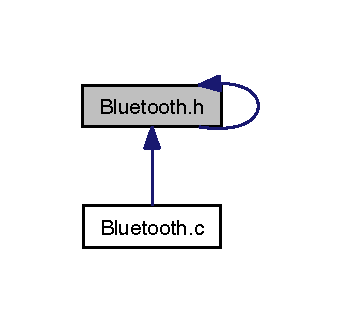
\includegraphics[width=164pt]{Bluetooth_8h__dep__incl}
\end{center}
\end{figure}
\subsection*{Data Structures}
\begin{DoxyCompactItemize}
\item 
struct {\bf Bluetooth}
\begin{DoxyCompactList}\small\item\em Bluetooth 모듈에 대한 구조체이다. Bluetooth 모듈은 다양한 방식으로 Bluetooth 통신을 할 수 있다. \end{DoxyCompactList}\item 
struct {\bf Bluetooth\-Extends}
\end{DoxyCompactItemize}
\subsection*{Functions}
\begin{DoxyCompactItemize}
\item 
const char $\ast$ {\bf Bluetooth\-Error\-Check} (int err\-Code)
\begin{DoxyCompactList}\small\item\em Bluetooth A\-P\-I에서 발생하는 Error Code들을 확인 해준다. \end{DoxyCompactList}\item 
Bluetooth {\bf New\-Bluetooth} (void)
\begin{DoxyCompactList}\small\item\em 새로운 Bluetooth 객체를 생성한다. \end{DoxyCompactList}\item 
void {\bf Destroy\-Bluetooth} (Bluetooth this\-\_\-gen)
\begin{DoxyCompactList}\small\item\em 생성한 Bluetooth 객체를 소멸 시킨다. \end{DoxyCompactList}\item 
bool {\bf is\-Bluetooth\-Accessible} (Bluetooth this\-\_\-gen)
\begin{DoxyCompactList}\small\item\em 현재 Bluetooth 기능 지원 여부를 반환 한다. \end{DoxyCompactList}\item 
bool {\bf on\-Bluetooth\-Connect} (Bluetooth this\-\_\-gen)
\begin{DoxyCompactList}\small\item\em Bluetooth기기로 연결을 시도하며 이의 성공 여부를 반환한다. \end{DoxyCompactList}\item 
bool {\bf is\-Bluetooth\-Connected} (Bluetooth this\-\_\-gen)
\begin{DoxyCompactList}\small\item\em Bluetooth기기와의 연결 상태를 확인한다. \end{DoxyCompactList}\item 
bool {\bf on\-Bluetooth\-Disconnect} (Bluetooth this\-\_\-gen)
\begin{DoxyCompactList}\small\item\em Bluetooth기기로 연결을 해제하며 이의 성공 여부를 반환한다. \end{DoxyCompactList}\item 
bool {\bf Bluetooth\-File\-Send} (Bluetooth this\-\_\-gen, String sendbuffer)
\begin{DoxyCompactList}\small\item\em Bluetooth기기로 데이터를 송신한다. \end{DoxyCompactList}\item 
bool {\bf Bluetooth\-File\-Recv} (Bluetooth this\-\_\-gen, String $\ast$recv\-Buffer)
\begin{DoxyCompactList}\small\item\em Bluetooth기기로 부터 데이터를 수신한다. \end{DoxyCompactList}\end{DoxyCompactItemize}


\subsection{Detailed Description}
Bluetooth A\-P\-I 를 사용하기 위해 포함해야 하는 헤더이다. \begin{DoxyNote}{Note}
Bluetooth의 is\-Accessible / on\-Connect / is\-Connected / on\-Disconnect / File\-Send / File\-Recv A\-P\-I를 제공한다. 
\end{DoxyNote}
\begin{DoxySeeAlso}{See Also}
{\tt Tizen Native A\-P\-I} 
\end{DoxySeeAlso}


\subsection{Data Structure Documentation}
\index{Bluetooth\-Extends@{Bluetooth\-Extends}}\label{structBluetoothExtends}
\subsubsection{struct Bluetooth\-Extends}


Collaboration diagram for Bluetooth\-Extends\-:
\nopagebreak
\begin{figure}[H]
\begin{center}
\leavevmode
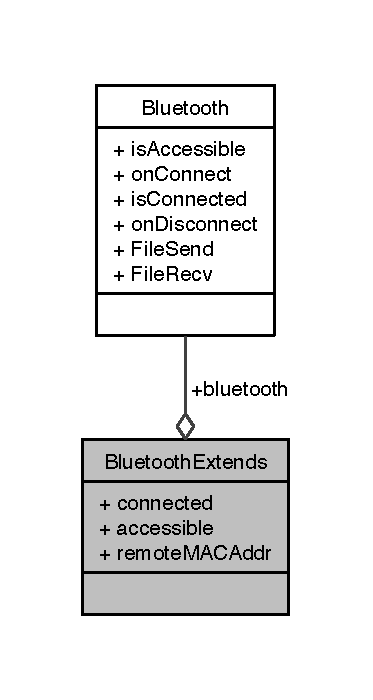
\includegraphics[width=179pt]{structBluetoothExtends__coll__graph}
\end{center}
\end{figure}
\begin{DoxyFields}{Data Fields}
bool\label{Bluetooth_8h_aab289e7470c5f2b7c5c35176418bae58}
&
accessible&
\\
\hline

struct {\bf \-\_\-\-Bluetooth}\label{Bluetooth_8h_a2988c3ea61c07f204d31abe492d8c4bd}
&
bluetooth&
\\
\hline

bool\label{Bluetooth_8h_ab98405f37820fcedb613ae4a9bee2708}
&
connected&
\\
\hline

String\label{Bluetooth_8h_a17bcb4936e21d1f61086e6287b555978}
&
remote\-M\-A\-C\-Addr&
\\
\hline

\end{DoxyFields}


\subsection{Function Documentation}
\index{Bluetooth.\-h@{Bluetooth.\-h}!Bluetooth\-Error\-Check@{Bluetooth\-Error\-Check}}
\index{Bluetooth\-Error\-Check@{Bluetooth\-Error\-Check}!Bluetooth.h@{Bluetooth.\-h}}
\subsubsection[{Bluetooth\-Error\-Check}]{\setlength{\rightskip}{0pt plus 5cm}const char $\ast$ Bluetooth\-Error\-Check (
\begin{DoxyParamCaption}
\item[{int}]{err\-Code}
\end{DoxyParamCaption}
)}\label{Bluetooth_8h_ab96c1e2bc34b5ecaeed60405ffbca5df}


Bluetooth A\-P\-I에서 발생하는 Error Code들을 확인 해준다. 


\begin{DoxyParams}[1]{Parameters}
\mbox{\tt in}  & {\em err\-Code} & 확인 하고자 하는 Error Code \\
\hline
\mbox{\tt out}  & {\em null} & \\
\hline
\end{DoxyParams}

\begin{DoxyRetVals}{Return values}
{\em B\-T\-\_\-\-E\-R\-R\-O\-R\-\_\-\-N\-O\-N\-E} & \-: Successful \\
\hline
{\em B\-T\-\_\-\-E\-R\-R\-O\-R\-\_\-\-C\-A\-N\-C\-E\-L\-L\-E\-D} & \-: Operation cancelled \\
\hline
{\em B\-T\-\_\-\-E\-R\-R\-O\-R\-\_\-\-I\-N\-V\-A\-L\-I\-D\-\_\-\-P\-A\-R\-A\-M\-E\-T\-E\-R} & \-: Invalid parameter \\
\hline
{\em B\-T\-\_\-\-E\-R\-R\-O\-R\-\_\-\-O\-U\-T\-\_\-\-O\-F\-\_\-\-M\-E\-M\-O\-R\-Y} & \-: Out of memory \\
\hline
{\em B\-T\-\_\-\-E\-R\-R\-O\-R\-\_\-\-R\-E\-S\-O\-U\-R\-C\-E\-\_\-\-B\-U\-S\-Y} & \-: Device or resource busy \\
\hline
{\em B\-T\-\_\-\-E\-R\-R\-O\-R\-\_\-\-T\-I\-M\-E\-D\-\_\-\-O\-U\-T} & \-: Timeout error \\
\hline
{\em B\-T\-\_\-\-E\-R\-R\-O\-R\-\_\-\-N\-O\-W\-\_\-\-I\-N\-\_\-\-P\-R\-O\-G\-R\-E\-S\-S} & \-: Operation now in progress \\
\hline
{\em B\-T\-\_\-\-E\-R\-R\-O\-R\-\_\-\-N\-O\-T\-\_\-\-S\-U\-P\-P\-O\-R\-T\-E\-D} & \-: Not Supported \\
\hline
{\em B\-T\-\_\-\-E\-R\-R\-O\-R\-\_\-\-P\-E\-R\-M\-I\-S\-S\-I\-O\-N\-\_\-\-D\-E\-N\-I\-E\-D} & \-: Permission denied \\
\hline
{\em B\-T\-\_\-\-E\-R\-R\-O\-R\-\_\-\-Q\-U\-O\-T\-A\-\_\-\-E\-X\-C\-E\-E\-D\-E\-D} & \-: Quota exceeded \\
\hline
{\em B\-T\-\_\-\-E\-R\-R\-O\-R\-\_\-\-N\-O\-T\-\_\-\-I\-N\-I\-T\-I\-A\-L\-I\-Z\-E\-D} & \-: Local adapter not initialized \\
\hline
{\em B\-T\-\_\-\-E\-R\-R\-O\-R\-\_\-\-N\-O\-T\-\_\-\-E\-N\-A\-B\-L\-E\-D} & \-: Local adapter not enabled \\
\hline
{\em B\-T\-\_\-\-E\-R\-R\-O\-R\-\_\-\-A\-L\-R\-E\-A\-D\-Y\-\_\-\-D\-O\-N\-E} & \-: Operation already done \\
\hline
{\em B\-T\-\_\-\-E\-R\-R\-O\-R\-\_\-\-O\-P\-E\-R\-A\-T\-I\-O\-N\-\_\-\-F\-A\-I\-L\-E\-D} & \-: Operation failed \\
\hline
{\em B\-T\-\_\-\-E\-R\-R\-O\-R\-\_\-\-N\-O\-T\-\_\-\-I\-N\-\_\-\-P\-R\-O\-G\-R\-E\-S\-S} & \-: Operation not in progress \\
\hline
{\em B\-T\-\_\-\-E\-R\-R\-O\-R\-\_\-\-R\-E\-M\-O\-T\-E\-\_\-\-D\-E\-V\-I\-C\-E\-\_\-\-N\-O\-T\-\_\-\-B\-O\-N\-D\-E\-D} & \-: Remote device not bonded \\
\hline
{\em B\-T\-\_\-\-E\-R\-R\-O\-R\-\_\-\-A\-U\-T\-H\-\_\-\-R\-E\-J\-E\-C\-T\-E\-D} & \-: Authentication rejected \\
\hline
{\em B\-T\-\_\-\-E\-R\-R\-O\-R\-\_\-\-A\-U\-T\-H\-\_\-\-F\-A\-I\-L\-E\-D} & \-: Authentication failed \\
\hline
{\em B\-T\-\_\-\-E\-R\-R\-O\-R\-\_\-\-R\-E\-M\-O\-T\-E\-\_\-\-D\-E\-V\-I\-C\-E\-\_\-\-N\-O\-T\-\_\-\-F\-O\-U\-N\-D} & \-: Remote device not found \\
\hline
{\em B\-T\-\_\-\-E\-R\-R\-O\-R\-\_\-\-S\-E\-R\-V\-I\-C\-E\-\_\-\-S\-E\-A\-R\-C\-H\-\_\-\-F\-A\-I\-L\-E\-D} & \-: Service search failed \\
\hline
{\em B\-T\-\_\-\-E\-R\-R\-O\-R\-\_\-\-R\-E\-M\-O\-T\-E\-\_\-\-D\-E\-V\-I\-C\-E\-\_\-\-N\-O\-T\-\_\-\-C\-O\-N\-N\-E\-C\-T\-E\-D} & \-: Remote device is not connected \\
\hline
{\em B\-T\-\_\-\-E\-R\-R\-O\-R\-\_\-\-A\-G\-A\-I\-N} & \-: Resource temporarily unavailable \\
\hline
{\em B\-T\-\_\-\-E\-R\-R\-O\-R\-\_\-\-S\-E\-R\-V\-I\-C\-E\-\_\-\-N\-O\-T\-\_\-\-F\-O\-U\-N\-D} & \-: Service Not Found \\
\hline
{\em B\-T\-\_\-\-E\-R\-R\-O\-R\-\_\-\-U\-N\-K\-N\-W\-O\-N} & \-: Unknown error occurred \\
\hline
\end{DoxyRetVals}
\begin{DoxyNote}{Note}
Bluetooth A\-P\-I에서 발생하는 Error Code들을 확인 해준다. \par
 Error의 내용은 Log를 통해 출력 된다. \par
 24가지의 Error Code들을 확인 가능 하다. 
\end{DoxyNote}
\begin{DoxySeeAlso}{See Also}
{\tt Tizen Native A\-P\-I Document -\/ Bluetooth part} 
\end{DoxySeeAlso}


Here is the caller graph for this function\-:
\nopagebreak
\begin{figure}[H]
\begin{center}
\leavevmode
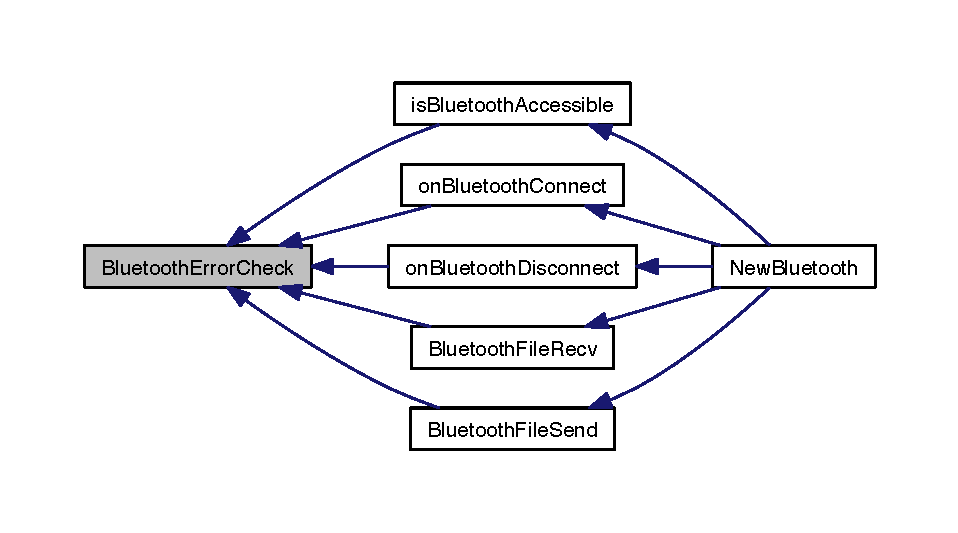
\includegraphics[width=350pt]{Bluetooth_8h_ab96c1e2bc34b5ecaeed60405ffbca5df_icgraph}
\end{center}
\end{figure}


\index{Bluetooth.\-h@{Bluetooth.\-h}!Bluetooth\-File\-Recv@{Bluetooth\-File\-Recv}}
\index{Bluetooth\-File\-Recv@{Bluetooth\-File\-Recv}!Bluetooth.h@{Bluetooth.\-h}}
\subsubsection[{Bluetooth\-File\-Recv}]{\setlength{\rightskip}{0pt plus 5cm}bool Bluetooth\-File\-Recv (
\begin{DoxyParamCaption}
\item[{Bluetooth}]{this\-\_\-gen, }
\item[{String $\ast$}]{recv\-Buffer}
\end{DoxyParamCaption}
)}\label{Bluetooth_8h_a43d4d767fbb4f0a1568a453e7b6a9995}


Bluetooth기기로 부터 데이터를 수신한다. 


\begin{DoxyParams}[1]{Parameters}
\mbox{\tt in}  & {\em this\-\_\-gen} & 데이터를 수신할 Bluetooth 객체 \\
\hline
\mbox{\tt in}  & {\em recv\-Buffer} & 수신할 데이터 주소 \\
\hline
\mbox{\tt out}  & {\em recv\-Buffer} & 수신한 데이터 \\
\hline
\end{DoxyParams}

\begin{DoxyRetVals}{Return values}
{\em bool} & \par
 함수의 성공 여부를 반환한다. \par
 실패시 {\ttfamily false를} 반환하며 상세한 원인을 Log로 출력한다. \\
\hline
\end{DoxyRetVals}
\begin{DoxyNote}{Note}
Bluetooth기기로 부터 데이터를 수신한다. 
\end{DoxyNote}
\begin{DoxySeeAlso}{See Also}
\doxyref{New\-Bluetooth}{p.}{Bluetooth_8h_aedecb2f1b25b6d408a1880978b66712a} \par
 \doxyref{Destroy\-Bluetooth}{p.}{Bluetooth_8h_a643b6a392ddbcf1c02bcfeb15ca52df8} \par
 \doxyref{is\-Bluetooth\-Accessible}{p.}{Bluetooth_8h_a00b401ae906bf1d77f232c88a14314fc} \par
 \doxyref{on\-Bluetooth\-Connect}{p.}{Bluetooth_8h_a77d0c6bf9a2f45a43a3b5801dd978fb6} \par
 \doxyref{is\-Bluetooth\-Connected}{p.}{Bluetooth_8h_a4959b3be5e12c0d3e4cc317e00e4621e} \par
 \doxyref{on\-Bluetooth\-Disconnect}{p.}{Bluetooth_8h_a26f809a19ded06421baab533eb8a59a6} \par
 \doxyref{Bluetooth\-File\-Send}{p.}{Bluetooth_8h_a169790dd12357103f392285063a4cfb9} 
\end{DoxySeeAlso}
\begin{DoxyPrecond}{Precondition}
{\bfseries feature} \par

\begin{DoxyItemize}
\item {\tt http\-://tizen.\-org/feature/network.\-bluetooth} 
\end{DoxyItemize}
\end{DoxyPrecond}


Here is the call graph for this function\-:
\nopagebreak
\begin{figure}[H]
\begin{center}
\leavevmode
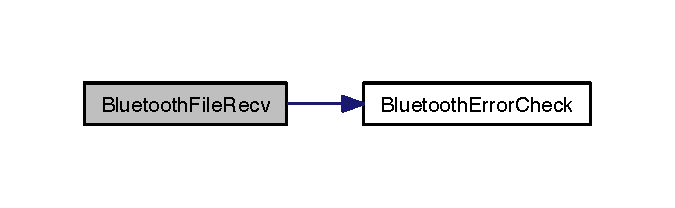
\includegraphics[width=324pt]{Bluetooth_8h_a43d4d767fbb4f0a1568a453e7b6a9995_cgraph}
\end{center}
\end{figure}




Here is the caller graph for this function\-:
\nopagebreak
\begin{figure}[H]
\begin{center}
\leavevmode
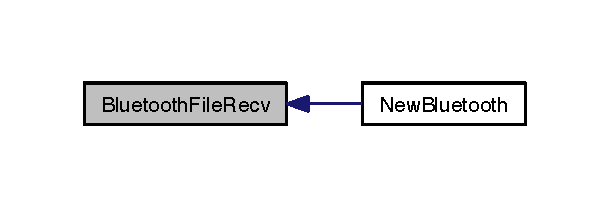
\includegraphics[width=292pt]{Bluetooth_8h_a43d4d767fbb4f0a1568a453e7b6a9995_icgraph}
\end{center}
\end{figure}


\index{Bluetooth.\-h@{Bluetooth.\-h}!Bluetooth\-File\-Send@{Bluetooth\-File\-Send}}
\index{Bluetooth\-File\-Send@{Bluetooth\-File\-Send}!Bluetooth.h@{Bluetooth.\-h}}
\subsubsection[{Bluetooth\-File\-Send}]{\setlength{\rightskip}{0pt plus 5cm}bool Bluetooth\-File\-Send (
\begin{DoxyParamCaption}
\item[{Bluetooth}]{this\-\_\-gen, }
\item[{String}]{sendbuffer}
\end{DoxyParamCaption}
)}\label{Bluetooth_8h_a169790dd12357103f392285063a4cfb9}


Bluetooth기기로 데이터를 송신한다. 


\begin{DoxyParams}[1]{Parameters}
\mbox{\tt in}  & {\em this\-\_\-gen} & 데이터를 송신할 Bluetooth 객체 \\
\hline
\mbox{\tt in}  & {\em sendbuffer} & 송신할 파일 path \\
\hline
\mbox{\tt out}  & {\em null} & \\
\hline
\end{DoxyParams}

\begin{DoxyRetVals}{Return values}
{\em bool} & \par
 함수의 성공 여부를 반환한다. \par
 실패시 {\ttfamily false를} 반환하며 상세한 원인을 Log로 출력한다. \\
\hline
\end{DoxyRetVals}
\begin{DoxyNote}{Note}
Bluetooth기기로 데이터를 송신한다. \par

\end{DoxyNote}
\begin{DoxySeeAlso}{See Also}
\doxyref{New\-Bluetooth}{p.}{Bluetooth_8h_aedecb2f1b25b6d408a1880978b66712a} \par
 \doxyref{Destroy\-Bluetooth}{p.}{Bluetooth_8h_a643b6a392ddbcf1c02bcfeb15ca52df8} \par
 \doxyref{is\-Bluetooth\-Accessible}{p.}{Bluetooth_8h_a00b401ae906bf1d77f232c88a14314fc} \par
 \doxyref{on\-Bluetooth\-Connect}{p.}{Bluetooth_8h_a77d0c6bf9a2f45a43a3b5801dd978fb6} \par
 \doxyref{is\-Bluetooth\-Connected}{p.}{Bluetooth_8h_a4959b3be5e12c0d3e4cc317e00e4621e} \par
 \doxyref{on\-Bluetooth\-Disconnect}{p.}{Bluetooth_8h_a26f809a19ded06421baab533eb8a59a6} \par
 \doxyref{Bluetooth\-File\-Recv}{p.}{Bluetooth_8h_a43d4d767fbb4f0a1568a453e7b6a9995} 
\end{DoxySeeAlso}
\begin{DoxyPrecond}{Precondition}
{\bfseries feature} \par

\begin{DoxyItemize}
\item {\tt http\-://tizen.\-org/feature/network.\-bluetooth} 
\end{DoxyItemize}
\end{DoxyPrecond}


Here is the call graph for this function\-:
\nopagebreak
\begin{figure}[H]
\begin{center}
\leavevmode
\includegraphics[width=324pt]{Bluetooth_8h_a169790dd12357103f392285063a4cfb9_cgraph}
\end{center}
\end{figure}




Here is the caller graph for this function\-:
\nopagebreak
\begin{figure}[H]
\begin{center}
\leavevmode
\includegraphics[width=292pt]{Bluetooth_8h_a169790dd12357103f392285063a4cfb9_icgraph}
\end{center}
\end{figure}


\index{Bluetooth.\-h@{Bluetooth.\-h}!Destroy\-Bluetooth@{Destroy\-Bluetooth}}
\index{Destroy\-Bluetooth@{Destroy\-Bluetooth}!Bluetooth.h@{Bluetooth.\-h}}
\subsubsection[{Destroy\-Bluetooth}]{\setlength{\rightskip}{0pt plus 5cm}void Destroy\-Bluetooth (
\begin{DoxyParamCaption}
\item[{Bluetooth}]{this\-\_\-gen}
\end{DoxyParamCaption}
)}\label{Bluetooth_8h_a643b6a392ddbcf1c02bcfeb15ca52df8}


생성한 Bluetooth 객체를 소멸 시킨다. 


\begin{DoxyParams}[1]{Parameters}
\mbox{\tt in}  & {\em this\-\_\-gen} & 소멸시킬 Bluetooth 객체 \\
\hline
\mbox{\tt out}  & {\em null} & \\
\hline
\end{DoxyParams}

\begin{DoxyRetVals}{Return values}
{\em void} & \\
\hline
\end{DoxyRetVals}
\begin{DoxyNote}{Note}
생성한 Bluetooth 객체를 소멸 시킨다. \par
 Bluetooth 객체를 사용한 후 반드시 호출해야 한다. 
\end{DoxyNote}
\begin{DoxySeeAlso}{See Also}
\doxyref{New\-Bluetooth}{p.}{Bluetooth_8h_aedecb2f1b25b6d408a1880978b66712a} 
\end{DoxySeeAlso}
\begin{DoxyPrecond}{Precondition}
{\bfseries feature} \par

\begin{DoxyItemize}
\item {\tt http\-://tizen.\-org/feature/network.\-bluetooth} 
\end{DoxyItemize}
\end{DoxyPrecond}
\index{Bluetooth.\-h@{Bluetooth.\-h}!is\-Bluetooth\-Accessible@{is\-Bluetooth\-Accessible}}
\index{is\-Bluetooth\-Accessible@{is\-Bluetooth\-Accessible}!Bluetooth.h@{Bluetooth.\-h}}
\subsubsection[{is\-Bluetooth\-Accessible}]{\setlength{\rightskip}{0pt plus 5cm}bool is\-Bluetooth\-Accessible (
\begin{DoxyParamCaption}
\item[{Bluetooth}]{this\-\_\-gen}
\end{DoxyParamCaption}
)}\label{Bluetooth_8h_a00b401ae906bf1d77f232c88a14314fc}


현재 Bluetooth 기능 지원 여부를 반환 한다. 


\begin{DoxyParams}[1]{Parameters}
\mbox{\tt in}  & {\em this\-\_\-gen} & 사용 가능 여부를 반환 할 Bluetooth 객체 \\
\hline
\mbox{\tt out}  & {\em null} & \\
\hline
\end{DoxyParams}

\begin{DoxyRetVals}{Return values}
{\em bool} & \par
 함수의 성공 여부를 반환한다. \par
 실패시 {\ttfamily false를} 반환하며 상세한 원인을 Log로 출력한다. \\
\hline
\end{DoxyRetVals}
\begin{DoxyNote}{Note}
현재 Bluetooth 기능 지원 여부를 반환 한다. \par
 지원 가능 이라면 {\ttfamily true}, 지원 가능이 아니라면 {\ttfamily false를} 반환한다. 
\end{DoxyNote}
\begin{DoxySeeAlso}{See Also}
\doxyref{New\-Bluetooth}{p.}{Bluetooth_8h_aedecb2f1b25b6d408a1880978b66712a} \par
 \doxyref{Destroy\-Bluetooth}{p.}{Bluetooth_8h_a643b6a392ddbcf1c02bcfeb15ca52df8} \par
 \doxyref{on\-Bluetooth\-Connect}{p.}{Bluetooth_8h_a77d0c6bf9a2f45a43a3b5801dd978fb6} \par
 \doxyref{is\-Bluetooth\-Connected}{p.}{Bluetooth_8h_a4959b3be5e12c0d3e4cc317e00e4621e} \par
 \doxyref{on\-Bluetooth\-Disconnect}{p.}{Bluetooth_8h_a26f809a19ded06421baab533eb8a59a6} \par
 \doxyref{Bluetooth\-File\-Send}{p.}{Bluetooth_8h_a169790dd12357103f392285063a4cfb9} \par
 \doxyref{Bluetooth\-File\-Recv}{p.}{Bluetooth_8h_a43d4d767fbb4f0a1568a453e7b6a9995} 
\end{DoxySeeAlso}
\begin{DoxyPrecond}{Precondition}
{\bfseries feature} \par

\begin{DoxyItemize}
\item {\tt http\-://tizen.\-org/feature/network.\-bluetooth} 
\end{DoxyItemize}
\end{DoxyPrecond}


Here is the call graph for this function\-:
\nopagebreak
\begin{figure}[H]
\begin{center}
\leavevmode
\includegraphics[width=340pt]{Bluetooth_8h_a00b401ae906bf1d77f232c88a14314fc_cgraph}
\end{center}
\end{figure}




Here is the caller graph for this function\-:
\nopagebreak
\begin{figure}[H]
\begin{center}
\leavevmode
\includegraphics[width=308pt]{Bluetooth_8h_a00b401ae906bf1d77f232c88a14314fc_icgraph}
\end{center}
\end{figure}


\index{Bluetooth.\-h@{Bluetooth.\-h}!is\-Bluetooth\-Connected@{is\-Bluetooth\-Connected}}
\index{is\-Bluetooth\-Connected@{is\-Bluetooth\-Connected}!Bluetooth.h@{Bluetooth.\-h}}
\subsubsection[{is\-Bluetooth\-Connected}]{\setlength{\rightskip}{0pt plus 5cm}bool is\-Bluetooth\-Connected (
\begin{DoxyParamCaption}
\item[{Bluetooth}]{this\-\_\-gen}
\end{DoxyParamCaption}
)}\label{Bluetooth_8h_a4959b3be5e12c0d3e4cc317e00e4621e}


Bluetooth기기와의 연결 상태를 확인한다. 


\begin{DoxyParams}[1]{Parameters}
\mbox{\tt in}  & {\em this\-\_\-gen} & 연결 상태를 확인할 Bluetooth 객체 \\
\hline
\mbox{\tt out}  & {\em null} & \\
\hline
\end{DoxyParams}

\begin{DoxyRetVals}{Return values}
{\em bool} & \par
 함수의 성공 여부를 반환한다. \par
 실패시 {\ttfamily false를} 반환하며 상세한 원인을 Log로 출력한다. \\
\hline
\end{DoxyRetVals}
\begin{DoxyNote}{Note}
Bluetooth기기와의 연결 상태를 확인한다. \par
 연결되어 있다면 {\ttfamily true}, 연결되어 있지 않다면 {\ttfamily false를} 반환한다. 
\end{DoxyNote}
\begin{DoxySeeAlso}{See Also}
\doxyref{New\-Bluetooth}{p.}{Bluetooth_8h_aedecb2f1b25b6d408a1880978b66712a} \par
 \doxyref{Destroy\-Bluetooth}{p.}{Bluetooth_8h_a643b6a392ddbcf1c02bcfeb15ca52df8} \par
 \doxyref{is\-Bluetooth\-Accessible}{p.}{Bluetooth_8h_a00b401ae906bf1d77f232c88a14314fc} \par
 \doxyref{on\-Bluetooth\-Connect}{p.}{Bluetooth_8h_a77d0c6bf9a2f45a43a3b5801dd978fb6} \par
 \doxyref{on\-Bluetooth\-Disconnect}{p.}{Bluetooth_8h_a26f809a19ded06421baab533eb8a59a6} \par
 \doxyref{Bluetooth\-File\-Send}{p.}{Bluetooth_8h_a169790dd12357103f392285063a4cfb9} \par
 \doxyref{Bluetooth\-File\-Recv}{p.}{Bluetooth_8h_a43d4d767fbb4f0a1568a453e7b6a9995} 
\end{DoxySeeAlso}
\begin{DoxyPrecond}{Precondition}
{\bfseries feature} \par

\begin{DoxyItemize}
\item {\tt http\-://tizen.\-org/feature/network.\-bluetooth} 
\end{DoxyItemize}
\end{DoxyPrecond}


Here is the caller graph for this function\-:
\nopagebreak
\begin{figure}[H]
\begin{center}
\leavevmode
\includegraphics[width=308pt]{Bluetooth_8h_a4959b3be5e12c0d3e4cc317e00e4621e_icgraph}
\end{center}
\end{figure}


\index{Bluetooth.\-h@{Bluetooth.\-h}!New\-Bluetooth@{New\-Bluetooth}}
\index{New\-Bluetooth@{New\-Bluetooth}!Bluetooth.h@{Bluetooth.\-h}}
\subsubsection[{New\-Bluetooth}]{\setlength{\rightskip}{0pt plus 5cm}Bluetooth New\-Bluetooth (
\begin{DoxyParamCaption}
\item[{void}]{}
\end{DoxyParamCaption}
)}\label{Bluetooth_8h_aedecb2f1b25b6d408a1880978b66712a}


새로운 Bluetooth 객체를 생성한다. 


\begin{DoxyParams}[1]{Parameters}
\mbox{\tt in}  & {\em void} & \\
\hline
\mbox{\tt out}  & {\em null} & \\
\hline
\end{DoxyParams}

\begin{DoxyRetVals}{Return values}
{\em Bluetooth} & \\
\hline
\end{DoxyRetVals}
\begin{DoxyNote}{Note}
새로운 Bluetooth 객체를 생성한다. \par
 Bluetooth 객체를 사용하기 전에 반드시 호출해야 한다. 
\end{DoxyNote}
\begin{DoxySeeAlso}{See Also}
\doxyref{Destroy\-Bluetooth}{p.}{Bluetooth_8h_a643b6a392ddbcf1c02bcfeb15ca52df8} \par
 \doxyref{is\-Bluetooth\-Accessible}{p.}{Bluetooth_8h_a00b401ae906bf1d77f232c88a14314fc} \par
 \doxyref{on\-Bluetooth\-Connect}{p.}{Bluetooth_8h_a77d0c6bf9a2f45a43a3b5801dd978fb6} \par
 \doxyref{is\-Bluetooth\-Connected}{p.}{Bluetooth_8h_a4959b3be5e12c0d3e4cc317e00e4621e} \par
 \doxyref{on\-Bluetooth\-Disconnect}{p.}{Bluetooth_8h_a26f809a19ded06421baab533eb8a59a6} \par
 \doxyref{Bluetooth\-File\-Send}{p.}{Bluetooth_8h_a169790dd12357103f392285063a4cfb9} \par
 \doxyref{Bluetooth\-File\-Recv}{p.}{Bluetooth_8h_a43d4d767fbb4f0a1568a453e7b6a9995} 
\end{DoxySeeAlso}
\begin{DoxyPrecond}{Precondition}
{\bfseries feature} \par

\begin{DoxyItemize}
\item {\tt http\-://tizen.\-org/feature/network.\-bluetooth} 
\end{DoxyItemize}
\end{DoxyPrecond}
\begin{DoxyWarning}{Warning}
사용이 끝났을 때 \doxyref{Destroy\-Bluetooth()}{p.}{Bluetooth_8h_a643b6a392ddbcf1c02bcfeb15ca52df8} 함수를 꼭 사용해야 한다.
\end{DoxyWarning}

\begin{DoxyCode}
Bluetooth NewBluetooth (\textcolor{keywordtype}{void})
\{
    BluetoothExtends * \textcolor{keyword}{this} = malloc (\textcolor{keyword}{sizeof} (BluetoothExtends));
    this->bluetooth.isAccessible = isBluetoothAccessible;
    this->bluetooth.onConnect    = onBluetoothConnect;
    this->bluetooth.isConnected  = isBluetoothConnected;
    this->bluetooth.onDisconnect = onBluetoothDisconnect;
    this->bluetooth.FileRecv     = BluetoothFileRecv;
    this->bluetooth.FileSend     = BluetoothFileSend;

    this->connected     = \textcolor{keyword}{false};
    this->accessible    = \textcolor{keyword}{false};
    this->remoteMACAddr = NULL;

    \textcolor{keywordflow}{return} &this->bluetooth;
\}
\end{DoxyCode}
 

Here is the call graph for this function\-:
\nopagebreak
\begin{figure}[H]
\begin{center}
\leavevmode
\includegraphics[width=350pt]{Bluetooth_8h_aedecb2f1b25b6d408a1880978b66712a_cgraph}
\end{center}
\end{figure}


\index{Bluetooth.\-h@{Bluetooth.\-h}!on\-Bluetooth\-Connect@{on\-Bluetooth\-Connect}}
\index{on\-Bluetooth\-Connect@{on\-Bluetooth\-Connect}!Bluetooth.h@{Bluetooth.\-h}}
\subsubsection[{on\-Bluetooth\-Connect}]{\setlength{\rightskip}{0pt plus 5cm}bool on\-Bluetooth\-Connect (
\begin{DoxyParamCaption}
\item[{Bluetooth}]{this\-\_\-gen}
\end{DoxyParamCaption}
)}\label{Bluetooth_8h_a77d0c6bf9a2f45a43a3b5801dd978fb6}


Bluetooth기기로 연결을 시도하며 이의 성공 여부를 반환한다. 


\begin{DoxyParams}[1]{Parameters}
\mbox{\tt in}  & {\em this\-\_\-gen} & 연결 성공 여부를 확인할 Bluetooth 객체 \\
\hline
\mbox{\tt out}  & {\em null} & \\
\hline
\end{DoxyParams}

\begin{DoxyRetVals}{Return values}
{\em bool} & \par
 함수의 성공 여부를 반환한다. \par
 실패시 {\ttfamily false를} 반환하며 상세한 원인을 Log로 출력한다. \\
\hline
\end{DoxyRetVals}
\begin{DoxyNote}{Note}
Bluetooth기기로 연결을 시도하며 이의 성공 여부를 반환한다. \par
 연결에 성공하면 {\ttfamily true}, 실패하면 {\ttfamily false를} 반환한다. 
\end{DoxyNote}
\begin{DoxySeeAlso}{See Also}
\doxyref{New\-Bluetooth}{p.}{Bluetooth_8h_aedecb2f1b25b6d408a1880978b66712a} \par
 \doxyref{Destroy\-Bluetooth}{p.}{Bluetooth_8h_a643b6a392ddbcf1c02bcfeb15ca52df8} \par
 \doxyref{is\-Bluetooth\-Accessible}{p.}{Bluetooth_8h_a00b401ae906bf1d77f232c88a14314fc} \par
 \doxyref{is\-Bluetooth\-Connected}{p.}{Bluetooth_8h_a4959b3be5e12c0d3e4cc317e00e4621e} \par
 \doxyref{on\-Bluetooth\-Disconnect}{p.}{Bluetooth_8h_a26f809a19ded06421baab533eb8a59a6} \par
 \doxyref{Bluetooth\-File\-Send}{p.}{Bluetooth_8h_a169790dd12357103f392285063a4cfb9} \par
 \doxyref{Bluetooth\-File\-Recv}{p.}{Bluetooth_8h_a43d4d767fbb4f0a1568a453e7b6a9995} 
\end{DoxySeeAlso}
\begin{DoxyPrecond}{Precondition}
{\bfseries feature} \par

\begin{DoxyItemize}
\item {\tt http\-://tizen.\-org/feature/network.\-bluetooth} 
\end{DoxyItemize}
\end{DoxyPrecond}


Here is the call graph for this function\-:
\nopagebreak
\begin{figure}[H]
\begin{center}
\leavevmode
\includegraphics[width=334pt]{Bluetooth_8h_a77d0c6bf9a2f45a43a3b5801dd978fb6_cgraph}
\end{center}
\end{figure}




Here is the caller graph for this function\-:
\nopagebreak
\begin{figure}[H]
\begin{center}
\leavevmode
\includegraphics[width=302pt]{Bluetooth_8h_a77d0c6bf9a2f45a43a3b5801dd978fb6_icgraph}
\end{center}
\end{figure}


\index{Bluetooth.\-h@{Bluetooth.\-h}!on\-Bluetooth\-Disconnect@{on\-Bluetooth\-Disconnect}}
\index{on\-Bluetooth\-Disconnect@{on\-Bluetooth\-Disconnect}!Bluetooth.h@{Bluetooth.\-h}}
\subsubsection[{on\-Bluetooth\-Disconnect}]{\setlength{\rightskip}{0pt plus 5cm}bool on\-Bluetooth\-Disconnect (
\begin{DoxyParamCaption}
\item[{Bluetooth}]{this\-\_\-gen}
\end{DoxyParamCaption}
)}\label{Bluetooth_8h_a26f809a19ded06421baab533eb8a59a6}


Bluetooth기기로 연결을 해제하며 이의 성공 여부를 반환한다. 


\begin{DoxyParams}[1]{Parameters}
\mbox{\tt in}  & {\em this\-\_\-gen} & 연결 해제 여부를 확인할 Bluetooth 객체 \\
\hline
\mbox{\tt out}  & {\em null} & \\
\hline
\end{DoxyParams}

\begin{DoxyRetVals}{Return values}
{\em bool} & \par
 함수의 성공 여부를 반환한다. \par
 실패시 {\ttfamily false를} 반환하며 상세한 원인을 Log로 출력한다. \\
\hline
\end{DoxyRetVals}
\begin{DoxyNote}{Note}
Bluetooth기기로 연결을 해제하며 이의 성공 여부를 반환한다. \par
 연결 해제에 성공하면 {\ttfamily true}, 실패하면 {\ttfamily false를} 반환한다. 
\end{DoxyNote}
\begin{DoxySeeAlso}{See Also}
\doxyref{New\-Bluetooth}{p.}{Bluetooth_8h_aedecb2f1b25b6d408a1880978b66712a} \par
 \doxyref{Destroy\-Bluetooth}{p.}{Bluetooth_8h_a643b6a392ddbcf1c02bcfeb15ca52df8} \par
 \doxyref{is\-Bluetooth\-Accessible}{p.}{Bluetooth_8h_a00b401ae906bf1d77f232c88a14314fc} \par
 \doxyref{on\-Bluetooth\-Connect}{p.}{Bluetooth_8h_a77d0c6bf9a2f45a43a3b5801dd978fb6} \par
 \doxyref{is\-Bluetooth\-Connected}{p.}{Bluetooth_8h_a4959b3be5e12c0d3e4cc317e00e4621e} \par
 \doxyref{Bluetooth\-File\-Send}{p.}{Bluetooth_8h_a169790dd12357103f392285063a4cfb9} \par
 \doxyref{Bluetooth\-File\-Recv}{p.}{Bluetooth_8h_a43d4d767fbb4f0a1568a453e7b6a9995} 
\end{DoxySeeAlso}
\begin{DoxyPrecond}{Precondition}
{\bfseries feature} \par

\begin{DoxyItemize}
\item {\tt http\-://tizen.\-org/feature/network.\-bluetooth} 
\end{DoxyItemize}
\end{DoxyPrecond}


Here is the call graph for this function\-:
\nopagebreak
\begin{figure}[H]
\begin{center}
\leavevmode
\includegraphics[width=346pt]{Bluetooth_8h_a26f809a19ded06421baab533eb8a59a6_cgraph}
\end{center}
\end{figure}




Here is the caller graph for this function\-:
\nopagebreak
\begin{figure}[H]
\begin{center}
\leavevmode
\includegraphics[width=314pt]{Bluetooth_8h_a26f809a19ded06421baab533eb8a59a6_icgraph}
\end{center}
\end{figure}



\section{Device\-Status.\-c File Reference}
\label{DeviceStatus_8c}\index{Device\-Status.\-c@{Device\-Status.\-c}}


Device Status A\-P\-I가 정의되어있다.  


{\ttfamily \#include \char`\"{}Device/\-Device\-Status.\-h\char`\"{}}\\*
{\ttfamily \#include $<$stdbool.\-h$>$}\\*
{\ttfamily \#include $<$stdlib.\-h$>$}\\*
{\ttfamily \#include $<$device/battery.\-h$>$}\\*
{\ttfamily \#include $<$device/display.\-h$>$}\\*
{\ttfamily \#include $<$device/led.\-h$>$}\\*
{\ttfamily \#include $<$device/haptic.\-h$>$}\\*
{\ttfamily \#include $<$dlog.\-h$>$}\\*
Include dependency graph for Device\-Status.\-c\-:\nopagebreak
\begin{figure}[H]
\begin{center}
\leavevmode
\includegraphics[width=350pt]{DeviceStatus_8c__incl}
\end{center}
\end{figure}
\subsection*{Functions}
\begin{DoxyCompactItemize}
\item 
const char $\ast$ {\bf Device\-Status\-Error\-Check} (int err\-Code)
\begin{DoxyCompactList}\small\item\em Device Status A\-P\-I에서 발생하는 Error Code들을 확인 해준다. \end{DoxyCompactList}\item 
Vibration {\bfseries New\-Vibration} (void)\label{DeviceStatus_8c_a9c3d84ca51a859ceb9eaa0097fa14266}

\item 
void {\bfseries Destroy\-Vibration} (Vibration this\-\_\-gen)\label{DeviceStatus_8c_a336e3f65421006097670aec144c07e4a}

\item 
bool {\bfseries Vibration\-Custom} (Vibration this\-\_\-gen, int period)\label{DeviceStatus_8c_ad72205770a47e2d00bb5615419665bc3}

\item 
bool {\bfseries Vibration\-Short} (Vibration this\-\_\-gen)\label{DeviceStatus_8c_a2a15fa61a394c104a130de94a49f81e9}

\item 
bool {\bfseries Vibration\-Middle} (Vibration this\-\_\-gen)\label{DeviceStatus_8c_ab12b6f187ca50d6e843c5c85c7d1e2c6}

\item 
bool {\bfseries Vibration\-Long} (Vibration this\-\_\-gen)\label{DeviceStatus_8c_aa7490eb5833cc7775d2da420a30b94fb}

\item 
Display {\bfseries New\-Display} (void)\label{DeviceStatus_8c_a239d9485c4000ae77b11e5f12378f95f}

\item 
void {\bfseries Destroy\-Display} (Display this\-\_\-gen)\label{DeviceStatus_8c_aa18ddc0342d1ca47145c759a8fa35d91}

\item 
bool {\bfseries Display\-Lock} (Display this\-\_\-gen)\label{DeviceStatus_8c_a45616f571bc7211e0749656b85b3baab}

\item 
bool {\bfseries Display\-Unlock} (Display this\-\_\-gen)\label{DeviceStatus_8c_a9e66aaebf66d63ec1555c4226f4154ca}

\item 
bool {\bfseries Display\-Dim} (Display this\-\_\-gen)\label{DeviceStatus_8c_a35d4bf5e52fdb81d5d8d83f8b22569b2}

\item 
int {\bfseries get\-Display\-Bright\-Level} (Display this\-\_\-gen)\label{DeviceStatus_8c_abf038dea7a71738b751dfdd3ce88ebf9}

\item 
bool {\bfseries set\-Display\-Bright\-Level} (Display this\-\_\-gen, int bright\-Level)\label{DeviceStatus_8c_a2ce601f6c832e1d4f587fec0a1ddaa86}

\item 
Battery {\bfseries New\-Battery} (void)\label{DeviceStatus_8c_a0fe7ab1f89e01e459f94bdecce693301}

\item 
void {\bfseries Destory\-Battery} (Battery this\-\_\-gen)\label{DeviceStatus_8c_a01b69d107b6708af6900d4279eeff281}

\item 
int {\bfseries get\-Battery\-Remains\-Percent} (Battery this\-\_\-gen)\label{DeviceStatus_8c_a983756d9f5b610b7d60c545546321b23}

\item 
bool {\bfseries is\-Battery\-Charging} (Battery this\-\_\-gen)\label{DeviceStatus_8c_af3fec730c212903458752e7fe4582636}

\item 
Flash {\bfseries New\-Flash} (void)\label{DeviceStatus_8c_a503e0814548cc9f370f87a3359187bff}

\item 
void {\bfseries Destory\-Flash} (Flash this\-\_\-gen)\label{DeviceStatus_8c_a4d0567730f41384d32902ef2b7c4b242}

\item 
bool {\bfseries on\-Flash} (void)\label{DeviceStatus_8c_a66766e7ced714f362745ea3c09eac6fc}

\item 
bool {\bfseries off\-Flash} (void)\label{DeviceStatus_8c_a7ab736323af55d4846ceec0dd746b4a4}

\end{DoxyCompactItemize}


\subsection{Detailed Description}
Device Status A\-P\-I가 정의되어있다. \begin{DoxyNote}{Note}
Device Status A\-P\-I가 정의되어있다. 
\end{DoxyNote}
\begin{DoxySeeAlso}{See Also}
\doxyref{Device\-Status.\-h}{p.}{DeviceStatus_8h} 
\end{DoxySeeAlso}


\subsection{Function Documentation}
\index{Device\-Status.\-c@{Device\-Status.\-c}!Device\-Status\-Error\-Check@{Device\-Status\-Error\-Check}}
\index{Device\-Status\-Error\-Check@{Device\-Status\-Error\-Check}!DeviceStatus.c@{Device\-Status.\-c}}
\subsubsection[{Device\-Status\-Error\-Check}]{\setlength{\rightskip}{0pt plus 5cm}const char$\ast$ Device\-Status\-Error\-Check (
\begin{DoxyParamCaption}
\item[{int}]{err\-Code}
\end{DoxyParamCaption}
)}\label{DeviceStatus_8c_a945d238478c332d3a5f212cd5b1f9946}


Device Status A\-P\-I에서 발생하는 Error Code들을 확인 해준다. 


\begin{DoxyParams}[1]{Parameters}
\mbox{\tt in}  & {\em err\-Code} & 확인 하고자 하는 Error Code \\
\hline
\mbox{\tt out}  & {\em null} & \\
\hline
\end{DoxyParams}

\begin{DoxyRetVals}{Return values}
{\em D\-E\-V\-I\-C\-E\-\_\-\-E\-R\-R\-O\-R\-\_\-\-N\-O\-N\-E} & \-: Successful \\
\hline
{\em D\-E\-V\-I\-C\-E\-\_\-\-E\-R\-R\-O\-R\-\_\-\-O\-P\-E\-R\-A\-T\-I\-O\-N\-\_\-\-F\-A\-I\-L\-E\-D} & \-: Operation not permitted \\
\hline
{\em D\-E\-V\-I\-C\-E\-\_\-\-E\-R\-R\-O\-R\-\_\-\-P\-E\-R\-M\-I\-S\-S\-I\-O\-N\-\_\-\-D\-E\-N\-I\-E\-D} & \-: Permission denied \\
\hline
{\em D\-E\-V\-I\-C\-E\-\_\-\-E\-R\-R\-O\-R\-\_\-\-I\-N\-V\-A\-L\-I\-D\-\_\-\-P\-A\-R\-A\-M\-E\-T\-E\-R} & \-: Invalid parameter \\
\hline
{\em D\-E\-V\-I\-C\-E\-\_\-\-E\-R\-R\-O\-R\-\_\-\-A\-L\-R\-E\-A\-D\-Y\-\_\-\-I\-N\-\_\-\-P\-R\-O\-G\-R\-E\-S\-S} & \-: Operation already in progress \\
\hline
{\em D\-E\-V\-I\-C\-E\-\_\-\-E\-R\-R\-O\-R\-\_\-\-N\-O\-T\-\_\-\-S\-U\-P\-P\-O\-R\-T\-E\-D} & \-: Not supported in this device \\
\hline
{\em D\-E\-V\-I\-C\-E\-\_\-\-E\-R\-R\-O\-R\-\_\-\-N\-O\-T\-\_\-\-I\-N\-I\-T\-I\-A\-L\-I\-Z\-E\-D} & \-: Not initialized \\
\hline
{\em D\-E\-V\-I\-C\-E\-\_\-\-E\-R\-R\-O\-R\-\_\-\-U\-N\-K\-N\-O\-W\-N} & \-: Unknown error occurred \\
\hline
\end{DoxyRetVals}
\begin{DoxyNote}{Note}
Device Status A\-P\-I에서 발생하는 Error Code들을 확인 해준다. \par
 Error의 내용은 Log를 통해 출력 된다. \par
 8가지의 Error Code들을 확인 가능 하다. 
\end{DoxyNote}
\begin{DoxySeeAlso}{See Also}
{\tt Tizen Native A\-P\-I Document -\/ Device Error} 
\end{DoxySeeAlso}

\section{Device\-Status.\-h File Reference}
\label{DeviceStatus_8h}\index{Device\-Status.\-h@{Device\-Status.\-h}}


Device Status A\-P\-I 를 사용하기 위해 포함해야 하는 헤더이다.  


{\ttfamily \#include $<$stdbool.\-h$>$}\\*
{\ttfamily \#include $<$stdalign.\-h$>$}\\*
{\ttfamily \#include \char`\"{}dit.\-h\char`\"{}}\\*
{\ttfamily \#include $<$device/display.\-h$>$}\\*
{\ttfamily \#include $<$device/haptic.\-h$>$}\\*
Include dependency graph for Device\-Status.\-h\-:
\nopagebreak
\begin{figure}[H]
\begin{center}
\leavevmode
\includegraphics[width=350pt]{DeviceStatus_8h__incl}
\end{center}
\end{figure}
This graph shows which files directly or indirectly include this file\-:
\nopagebreak
\begin{figure}[H]
\begin{center}
\leavevmode
\includegraphics[width=162pt]{DeviceStatus_8h__dep__incl}
\end{center}
\end{figure}
\subsection*{Data Structures}
\begin{DoxyCompactItemize}
\item 
struct {\bf Vibration}
\begin{DoxyCompactList}\small\item\em Vibration 모듈에 대한 구조체이다. Vibration 모듈은 다양한 방식으로 진동을 조절 할 수 있다. \end{DoxyCompactList}\item 
struct {\bf Vibration\-Extend}
\item 
struct {\bf Display}
\begin{DoxyCompactList}\small\item\em Display 모듈에 대한 구조체이다. Display 모듈은 다양한 방식으로 화면을 조절 할 수 있다. \end{DoxyCompactList}\end{DoxyCompactItemize}
\subsection*{Functions}
\begin{DoxyCompactItemize}
\item 
const char $\ast$ {\bf Device\-Status\-Error\-Check} (int err\-Code)
\begin{DoxyCompactList}\small\item\em Device Status A\-P\-I에서 발생하는 Error Code들을 확인 해준다. \end{DoxyCompactList}\item 
Vibration {\bf New\-Vibration} (void)
\begin{DoxyCompactList}\small\item\em 새로운 Vibration 객체를 생성한다. \end{DoxyCompactList}\item 
void {\bf Destroy\-Vibration} (Vibration this\-\_\-gen)
\begin{DoxyCompactList}\small\item\em 생성한 Vibration 객체를 소멸 시킨다. \end{DoxyCompactList}\item 
bool {\bf Vibration\-Custom} (Vibration this\-\_\-gen, int period)
\begin{DoxyCompactList}\small\item\em 사용자가 정의한 시간만큼 device를 진동 시킨다. \end{DoxyCompactList}\item 
bool {\bf Vibration\-Short} (Vibration this\-\_\-gen)
\begin{DoxyCompactList}\small\item\em 짧은 시간만큼 device를 진동 시킨다. ({\bfseries 0.\-1초}) \end{DoxyCompactList}\item 
bool {\bf Vibration\-Middle} (Vibration this\-\_\-gen)
\begin{DoxyCompactList}\small\item\em 중간 시간만큼 device를 진동 시킨다. ({\bfseries 0.\-5초}) \end{DoxyCompactList}\item 
bool {\bf Vibration\-Long} (Vibration this\-\_\-gen)
\begin{DoxyCompactList}\small\item\em 긴 시간만큼 device를 진동 시킨다. ({\bfseries 1.\-5초}) \end{DoxyCompactList}\end{DoxyCompactItemize}


\subsection{Detailed Description}
Device Status A\-P\-I 를 사용하기 위해 포함해야 하는 헤더이다. \begin{DoxyNote}{Note}
Device의 Vibration / Display / Battery / Flash 관련 A\-P\-I를 제공한다. 
\end{DoxyNote}
\begin{DoxySeeAlso}{See Also}
{\tt Tizen Native A\-P\-I} 
\end{DoxySeeAlso}


\subsection{Data Structure Documentation}
\index{Vibration\-Extend@{Vibration\-Extend}}\label{structVibrationExtend}
\subsubsection{struct Vibration\-Extend}


Collaboration diagram for Vibration\-Extend\-:
\nopagebreak
\begin{figure}[H]
\begin{center}
\leavevmode
\includegraphics[width=169pt]{structVibrationExtend__coll__graph}
\end{center}
\end{figure}
\begin{DoxyFields}{Data Fields}
haptic\-\_\-device\-\_\-h\label{DeviceStatus_8h_a63d0de000aa0d33eac6ea67cc3730d7b}
&
handle&
\\
\hline

struct {\bf \-\_\-\-Vibration}\label{DeviceStatus_8h_a166218f842ee2835fa6346df461fbfab}
&
vibration&
\\
\hline

\end{DoxyFields}


\subsection{Function Documentation}
\index{Device\-Status.\-h@{Device\-Status.\-h}!Destroy\-Vibration@{Destroy\-Vibration}}
\index{Destroy\-Vibration@{Destroy\-Vibration}!DeviceStatus.h@{Device\-Status.\-h}}
\subsubsection[{Destroy\-Vibration}]{\setlength{\rightskip}{0pt plus 5cm}void Destroy\-Vibration (
\begin{DoxyParamCaption}
\item[{Vibration}]{this\-\_\-gen}
\end{DoxyParamCaption}
)}\label{DeviceStatus_8h_a336e3f65421006097670aec144c07e4a}


생성한 Vibration 객체를 소멸 시킨다. 


\begin{DoxyParams}[1]{Parameters}
\mbox{\tt in}  & {\em this\-\_\-gen} & 소멸시킬 Vibration 객체 \\
\hline
\mbox{\tt out}  & {\em null} & \\
\hline
\end{DoxyParams}

\begin{DoxyRetVals}{Return values}
{\em void} & \\
\hline
\end{DoxyRetVals}
\begin{DoxyNote}{Note}
생성한 Vibration 객체를 소멸 시킨다. \par
 Vibration 객체를 사용한 후 반드시 호출해야 한다. 
\end{DoxyNote}
\begin{DoxySeeAlso}{See Also}
\doxyref{New\-Vibration}{p.}{DeviceStatus_8h_a9c3d84ca51a859ceb9eaa0097fa14266} 
\end{DoxySeeAlso}
\begin{DoxyPrecond}{Precondition}
{\bfseries privilege} \par

\begin{DoxyItemize}
\item {\tt http\-://tizen.\-org/privilege/haptic} 
\end{DoxyItemize}
\end{DoxyPrecond}
\index{Device\-Status.\-h@{Device\-Status.\-h}!Device\-Status\-Error\-Check@{Device\-Status\-Error\-Check}}
\index{Device\-Status\-Error\-Check@{Device\-Status\-Error\-Check}!DeviceStatus.h@{Device\-Status.\-h}}
\subsubsection[{Device\-Status\-Error\-Check}]{\setlength{\rightskip}{0pt plus 5cm}const char $\ast$ Device\-Status\-Error\-Check (
\begin{DoxyParamCaption}
\item[{int}]{err\-Code}
\end{DoxyParamCaption}
)}\label{DeviceStatus_8h_ab765e8bcaf98bf5f3c93b9e0fcc7e17c}


Device Status A\-P\-I에서 발생하는 Error Code들을 확인 해준다. 


\begin{DoxyParams}[1]{Parameters}
\mbox{\tt in}  & {\em err\-Code} & 확인 하고자 하는 Error Code \\
\hline
\mbox{\tt out}  & {\em null} & \\
\hline
\end{DoxyParams}

\begin{DoxyRetVals}{Return values}
{\em D\-E\-V\-I\-C\-E\-\_\-\-E\-R\-R\-O\-R\-\_\-\-N\-O\-N\-E} & \-: Successful \\
\hline
{\em D\-E\-V\-I\-C\-E\-\_\-\-E\-R\-R\-O\-R\-\_\-\-O\-P\-E\-R\-A\-T\-I\-O\-N\-\_\-\-F\-A\-I\-L\-E\-D} & \-: Operation not permitted \\
\hline
{\em D\-E\-V\-I\-C\-E\-\_\-\-E\-R\-R\-O\-R\-\_\-\-P\-E\-R\-M\-I\-S\-S\-I\-O\-N\-\_\-\-D\-E\-N\-I\-E\-D} & \-: Permission denied \\
\hline
{\em D\-E\-V\-I\-C\-E\-\_\-\-E\-R\-R\-O\-R\-\_\-\-I\-N\-V\-A\-L\-I\-D\-\_\-\-P\-A\-R\-A\-M\-E\-T\-E\-R} & \-: Invalid parameter \\
\hline
{\em D\-E\-V\-I\-C\-E\-\_\-\-E\-R\-R\-O\-R\-\_\-\-A\-L\-R\-E\-A\-D\-Y\-\_\-\-I\-N\-\_\-\-P\-R\-O\-G\-R\-E\-S\-S} & \-: Operation already in progress \\
\hline
{\em D\-E\-V\-I\-C\-E\-\_\-\-E\-R\-R\-O\-R\-\_\-\-N\-O\-T\-\_\-\-S\-U\-P\-P\-O\-R\-T\-E\-D} & \-: Not supported in this device \\
\hline
{\em D\-E\-V\-I\-C\-E\-\_\-\-E\-R\-R\-O\-R\-\_\-\-N\-O\-T\-\_\-\-I\-N\-I\-T\-I\-A\-L\-I\-Z\-E\-D} & \-: Not initialized \\
\hline
{\em D\-E\-V\-I\-C\-E\-\_\-\-E\-R\-R\-O\-R\-\_\-\-U\-N\-K\-N\-O\-W\-N} & \-: Unknown error occurred \\
\hline
\end{DoxyRetVals}
\begin{DoxyNote}{Note}
Device Status A\-P\-I에서 발생하는 Error Code들을 확인 해준다. \par
 Error의 내용은 Log를 통해 출력 된다. \par
 8가지의 Error Code들을 확인 가능 하다. 
\end{DoxyNote}
\begin{DoxySeeAlso}{See Also}
{\tt Tizen Native A\-P\-I Document -\/ Device Error} 
\end{DoxySeeAlso}


Here is the caller graph for this function\-:
\nopagebreak
\begin{figure}[H]
\begin{center}
\leavevmode
\includegraphics[width=350pt]{DeviceStatus_8h_ab765e8bcaf98bf5f3c93b9e0fcc7e17c_icgraph}
\end{center}
\end{figure}


\index{Device\-Status.\-h@{Device\-Status.\-h}!New\-Vibration@{New\-Vibration}}
\index{New\-Vibration@{New\-Vibration}!DeviceStatus.h@{Device\-Status.\-h}}
\subsubsection[{New\-Vibration}]{\setlength{\rightskip}{0pt plus 5cm}Vibration New\-Vibration (
\begin{DoxyParamCaption}
\item[{void}]{}
\end{DoxyParamCaption}
)}\label{DeviceStatus_8h_a9c3d84ca51a859ceb9eaa0097fa14266}


새로운 Vibration 객체를 생성한다. 


\begin{DoxyParams}[1]{Parameters}
\mbox{\tt in}  & {\em void} & \\
\hline
\mbox{\tt out}  & {\em null} & \\
\hline
\end{DoxyParams}

\begin{DoxyRetVals}{Return values}
{\em Vibration} & \\
\hline
\end{DoxyRetVals}
\begin{DoxyNote}{Note}
새로운 Vibration 객체를 생성한다. \par
 Vibration 객체를 사용하기 전에 반드시 호출해야 한다. 
\end{DoxyNote}
\begin{DoxySeeAlso}{See Also}
\doxyref{Destroy\-Vibration}{p.}{DeviceStatus_8h_a336e3f65421006097670aec144c07e4a} \par
 \doxyref{Vibration\-Custom}{p.}{DeviceStatus_8h_ad72205770a47e2d00bb5615419665bc3} \par
 \doxyref{Vibration\-Short}{p.}{DeviceStatus_8h_a2a15fa61a394c104a130de94a49f81e9} \par
 \doxyref{Vibration\-Middle}{p.}{DeviceStatus_8h_ab12b6f187ca50d6e843c5c85c7d1e2c6} \par
 \doxyref{Vibration\-Long}{p.}{DeviceStatus_8h_aa7490eb5833cc7775d2da420a30b94fb} 
\end{DoxySeeAlso}
\begin{DoxyPrecond}{Precondition}
{\bfseries privilege} \par

\begin{DoxyItemize}
\item {\tt http\-://tizen.\-org/privilege/haptic} 
\end{DoxyItemize}
\end{DoxyPrecond}
\begin{DoxyWarning}{Warning}
사용이 끝났을 때 \doxyref{Destroy\-Vibration()}{p.}{DeviceStatus_8h_a336e3f65421006097670aec144c07e4a} 함수를 꼭 사용해야 한다.
\end{DoxyWarning}

\begin{DoxyCode}
Vibration NewVibration (\textcolor{keywordtype}{void})
\{
    VibrationExtend * \textcolor{keyword}{this} = (VibrationExtend *)malloc (\textcolor{keyword}{sizeof} (VibrationExtend));

    this->vibration.Custom = VibrationCustom;
    this->vibration.Short  = VibrationShort;
    this->vibration.Middle = VibrationMiddle;
    this->vibration.Long   = VibrationLong;

   device\_haptic\_open (0, &this->handle);

    \textcolor{keywordflow}{return} &this->vibration;
\}
\end{DoxyCode}
 

Here is the call graph for this function\-:
\nopagebreak
\begin{figure}[H]
\begin{center}
\leavevmode
\includegraphics[width=350pt]{DeviceStatus_8h_a9c3d84ca51a859ceb9eaa0097fa14266_cgraph}
\end{center}
\end{figure}


\index{Device\-Status.\-h@{Device\-Status.\-h}!Vibration\-Custom@{Vibration\-Custom}}
\index{Vibration\-Custom@{Vibration\-Custom}!DeviceStatus.h@{Device\-Status.\-h}}
\subsubsection[{Vibration\-Custom}]{\setlength{\rightskip}{0pt plus 5cm}bool Vibration\-Custom (
\begin{DoxyParamCaption}
\item[{Vibration}]{this\-\_\-gen, }
\item[{int}]{period}
\end{DoxyParamCaption}
)}\label{DeviceStatus_8h_ad72205770a47e2d00bb5615419665bc3}


사용자가 정의한 시간만큼 device를 진동 시킨다. 


\begin{DoxyParams}[1]{Parameters}
\mbox{\tt in}  & {\em this\-\_\-gen} & 진동 시킬 Vibration 객체 \\
\hline
\mbox{\tt in}  & {\em period} & 진동 시킬 시간 ({\itshape Millisecond}) \\
\hline
\mbox{\tt out}  & {\em null} & \\
\hline
\end{DoxyParams}

\begin{DoxyRetVals}{Return values}
{\em bool} & \par
 함수의 성공 여부를 반환한다. \par
 실패시 {\ttfamily false를} 반환하며 상세한 원인을 Log로 출력한다. \\
\hline
\end{DoxyRetVals}
\begin{DoxyNote}{Note}
사용자가 정의한 {\ttfamily period} 만큼 device를 진동시킨다. \par
 시간 단위는 {\itshape Millisecond} 이다. 
\end{DoxyNote}
\begin{DoxySeeAlso}{See Also}
\doxyref{New\-Vibration}{p.}{DeviceStatus_8h_a9c3d84ca51a859ceb9eaa0097fa14266} \par
 \doxyref{Vibration\-Short}{p.}{DeviceStatus_8h_a2a15fa61a394c104a130de94a49f81e9} \par
 \doxyref{Vibration\-Middle}{p.}{DeviceStatus_8h_ab12b6f187ca50d6e843c5c85c7d1e2c6} \par
 \doxyref{Vibration\-Long}{p.}{DeviceStatus_8h_aa7490eb5833cc7775d2da420a30b94fb} 
\end{DoxySeeAlso}
\begin{DoxyPrecond}{Precondition}
{\bfseries privilege} \par

\begin{DoxyItemize}
\item {\tt http\-://tizen.\-org/privilege/haptic} 
\end{DoxyItemize}
\end{DoxyPrecond}


Here is the call graph for this function\-:
\nopagebreak
\begin{figure}[H]
\begin{center}
\leavevmode
\includegraphics[width=332pt]{DeviceStatus_8h_ad72205770a47e2d00bb5615419665bc3_cgraph}
\end{center}
\end{figure}




Here is the caller graph for this function\-:
\nopagebreak
\begin{figure}[H]
\begin{center}
\leavevmode
\includegraphics[width=282pt]{DeviceStatus_8h_ad72205770a47e2d00bb5615419665bc3_icgraph}
\end{center}
\end{figure}


\index{Device\-Status.\-h@{Device\-Status.\-h}!Vibration\-Long@{Vibration\-Long}}
\index{Vibration\-Long@{Vibration\-Long}!DeviceStatus.h@{Device\-Status.\-h}}
\subsubsection[{Vibration\-Long}]{\setlength{\rightskip}{0pt plus 5cm}bool Vibration\-Long (
\begin{DoxyParamCaption}
\item[{Vibration}]{this\-\_\-gen}
\end{DoxyParamCaption}
)}\label{DeviceStatus_8h_aa7490eb5833cc7775d2da420a30b94fb}


긴 시간만큼 device를 진동 시킨다. ({\bfseries 1.\-5초}) 


\begin{DoxyParams}[1]{Parameters}
\mbox{\tt in}  & {\em this\-\_\-gen} & 진동 시킬 Vibration 객체 \\
\hline
\mbox{\tt out}  & {\em null} & \\
\hline
\end{DoxyParams}

\begin{DoxyRetVals}{Return values}
{\em bool} & \par
 함수의 성공 여부를 반환한다. \par
 실패시 {\ttfamily false를} 반환하며 상세한 원인을 Log로 출력한다. \\
\hline
\end{DoxyRetVals}
\begin{DoxyNote}{Note}
긴 시간만큼 device를 진동 시킨다. ({\bfseries 1.\-5초}) 
\end{DoxyNote}
\begin{DoxySeeAlso}{See Also}
\doxyref{New\-Vibration}{p.}{DeviceStatus_8h_a9c3d84ca51a859ceb9eaa0097fa14266} \par
 \doxyref{Vibration\-Custom}{p.}{DeviceStatus_8h_ad72205770a47e2d00bb5615419665bc3} \par
 \doxyref{Vibration\-Short}{p.}{DeviceStatus_8h_a2a15fa61a394c104a130de94a49f81e9} \par
 \doxyref{Vibration\-Middle}{p.}{DeviceStatus_8h_ab12b6f187ca50d6e843c5c85c7d1e2c6} 
\end{DoxySeeAlso}
\begin{DoxyPrecond}{Precondition}
{\bfseries privilege} \par

\begin{DoxyItemize}
\item {\tt http\-://tizen.\-org/privilege/haptic} 
\end{DoxyItemize}
\end{DoxyPrecond}


Here is the call graph for this function\-:
\nopagebreak
\begin{figure}[H]
\begin{center}
\leavevmode
\includegraphics[width=320pt]{DeviceStatus_8h_aa7490eb5833cc7775d2da420a30b94fb_cgraph}
\end{center}
\end{figure}




Here is the caller graph for this function\-:
\nopagebreak
\begin{figure}[H]
\begin{center}
\leavevmode
\includegraphics[width=270pt]{DeviceStatus_8h_aa7490eb5833cc7775d2da420a30b94fb_icgraph}
\end{center}
\end{figure}


\index{Device\-Status.\-h@{Device\-Status.\-h}!Vibration\-Middle@{Vibration\-Middle}}
\index{Vibration\-Middle@{Vibration\-Middle}!DeviceStatus.h@{Device\-Status.\-h}}
\subsubsection[{Vibration\-Middle}]{\setlength{\rightskip}{0pt plus 5cm}bool Vibration\-Middle (
\begin{DoxyParamCaption}
\item[{Vibration}]{this\-\_\-gen}
\end{DoxyParamCaption}
)}\label{DeviceStatus_8h_ab12b6f187ca50d6e843c5c85c7d1e2c6}


중간 시간만큼 device를 진동 시킨다. ({\bfseries 0.\-5초}) 


\begin{DoxyParams}[1]{Parameters}
\mbox{\tt in}  & {\em this\-\_\-gen} & 진동 시킬 Vibration 객체 \\
\hline
\mbox{\tt out}  & {\em null} & \\
\hline
\end{DoxyParams}

\begin{DoxyRetVals}{Return values}
{\em bool} & \par
 함수의 성공 여부를 반환한다. \par
 실패시 {\ttfamily false를} 반환하며 상세한 원인을 Log로 출력한다. \\
\hline
\end{DoxyRetVals}
\begin{DoxyNote}{Note}
중간 시간만큼 device를 진동 시킨다. ({\bfseries 0.\-5초}) 
\end{DoxyNote}
\begin{DoxySeeAlso}{See Also}
\doxyref{New\-Vibration}{p.}{DeviceStatus_8h_a9c3d84ca51a859ceb9eaa0097fa14266} \par
 \doxyref{Vibration\-Custom}{p.}{DeviceStatus_8h_ad72205770a47e2d00bb5615419665bc3} \par
 \doxyref{Vibration\-Short}{p.}{DeviceStatus_8h_a2a15fa61a394c104a130de94a49f81e9} \par
 \doxyref{Vibration\-Long}{p.}{DeviceStatus_8h_aa7490eb5833cc7775d2da420a30b94fb} 
\end{DoxySeeAlso}
\begin{DoxyPrecond}{Precondition}
{\bfseries privilege} \par

\begin{DoxyItemize}
\item {\tt http\-://tizen.\-org/privilege/haptic} 
\end{DoxyItemize}
\end{DoxyPrecond}


Here is the call graph for this function\-:
\nopagebreak
\begin{figure}[H]
\begin{center}
\leavevmode
\includegraphics[width=328pt]{DeviceStatus_8h_ab12b6f187ca50d6e843c5c85c7d1e2c6_cgraph}
\end{center}
\end{figure}




Here is the caller graph for this function\-:
\nopagebreak
\begin{figure}[H]
\begin{center}
\leavevmode
\includegraphics[width=278pt]{DeviceStatus_8h_ab12b6f187ca50d6e843c5c85c7d1e2c6_icgraph}
\end{center}
\end{figure}


\index{Device\-Status.\-h@{Device\-Status.\-h}!Vibration\-Short@{Vibration\-Short}}
\index{Vibration\-Short@{Vibration\-Short}!DeviceStatus.h@{Device\-Status.\-h}}
\subsubsection[{Vibration\-Short}]{\setlength{\rightskip}{0pt plus 5cm}bool Vibration\-Short (
\begin{DoxyParamCaption}
\item[{Vibration}]{this\-\_\-gen}
\end{DoxyParamCaption}
)}\label{DeviceStatus_8h_a2a15fa61a394c104a130de94a49f81e9}


짧은 시간만큼 device를 진동 시킨다. ({\bfseries 0.\-1초}) 


\begin{DoxyParams}[1]{Parameters}
\mbox{\tt in}  & {\em this\-\_\-gen} & 진동 시킬 Vibration 객체 \\
\hline
\mbox{\tt out}  & {\em null} & \\
\hline
\end{DoxyParams}

\begin{DoxyRetVals}{Return values}
{\em bool} & \par
 함수의 성공 여부를 반환한다. \par
 실패시 {\ttfamily false를} 반환하며 상세한 원인을 Log로 출력한다. \\
\hline
\end{DoxyRetVals}
\begin{DoxyNote}{Note}
짧은 시간만큼 device를 진동 시킨다. ({\bfseries 0.\-1초}) 
\end{DoxyNote}
\begin{DoxySeeAlso}{See Also}
\doxyref{New\-Vibration}{p.}{DeviceStatus_8h_a9c3d84ca51a859ceb9eaa0097fa14266} \par
 \doxyref{Vibration\-Custom}{p.}{DeviceStatus_8h_ad72205770a47e2d00bb5615419665bc3} \par
 \doxyref{Vibration\-Middle}{p.}{DeviceStatus_8h_ab12b6f187ca50d6e843c5c85c7d1e2c6} \par
 \doxyref{Vibration\-Long}{p.}{DeviceStatus_8h_aa7490eb5833cc7775d2da420a30b94fb} 
\end{DoxySeeAlso}
\begin{DoxyPrecond}{Precondition}
{\bfseries privilege} \par

\begin{DoxyItemize}
\item {\tt http\-://tizen.\-org/privilege/haptic} 
\end{DoxyItemize}
\end{DoxyPrecond}


Here is the call graph for this function\-:
\nopagebreak
\begin{figure}[H]
\begin{center}
\leavevmode
\includegraphics[width=322pt]{DeviceStatus_8h_a2a15fa61a394c104a130de94a49f81e9_cgraph}
\end{center}
\end{figure}




Here is the caller graph for this function\-:
\nopagebreak
\begin{figure}[H]
\begin{center}
\leavevmode
\includegraphics[width=272pt]{DeviceStatus_8h_a2a15fa61a394c104a130de94a49f81e9_icgraph}
\end{center}
\end{figure}



\section{dit.\-h File Reference}
\label{dit_8h}\index{dit.\-h@{dit.\-h}}


D\-I\-T Library를 통합 관리한다.  


{\ttfamily \#include $<$stdbool.\-h$>$}\\*
{\ttfamily \#include $<$stdalign.\-h$>$}\\*
{\ttfamily \#include $<$tizen.\-h$>$}\\*
Include dependency graph for dit.\-h\-:\nopagebreak
\begin{figure}[H]
\begin{center}
\leavevmode
\includegraphics[width=276pt]{dit_8h__incl}
\end{center}
\end{figure}
This graph shows which files directly or indirectly include this file\-:\nopagebreak
\begin{figure}[H]
\begin{center}
\leavevmode
\includegraphics[width=350pt]{dit_8h__dep__incl}
\end{center}
\end{figure}
\subsection*{Macros}
\begin{DoxyCompactItemize}
\item 
\#define {\bfseries D\-O\-W\-N\-L\-O\-A\-D\-S\-F\-O\-L\-D\-E\-R\-P\-A\-T\-H}~\char`\"{}/opt/usr/media/Downloads\char`\"{}\label{dit_8h_af029412212bf6a445500174d743cdd20}

\item 
\#define {\bfseries E\-X\-P\-O\-R\-T\-\_\-\-A\-P\-I}~\-\_\-\-\_\-attribute\-\_\-\-\_\-((\-\_\-\-\_\-visibility\-\_\-\-\_\-(\char`\"{}default\char`\"{})))\label{dit_8h_a3536620a51a6fa45b41e6d9ff6fc4ad3}

\end{DoxyCompactItemize}
\subsection*{Typedefs}
\begin{DoxyCompactItemize}
\item 
typedef char $\ast$ {\bfseries String}\label{dit_8h_a2efe6d463d80744789f228f5dc4baa39}

\end{DoxyCompactItemize}


\subsection{Detailed Description}
D\-I\-T Library를 통합 관리한다. \begin{DoxyNote}{Note}
T\-I\-Z\-E\-N A\-P\-I를 새롭게 Wrapping 하여서 Library형식으로 제공한다. 
\end{DoxyNote}
\begin{DoxySeeAlso}{See Also}
{\tt https\-://developer.\-tizen.\-org/dev-\/guide/2.\-3.\-0} 
\end{DoxySeeAlso}

\section{File.\-c File Reference}
\label{File_8c}\index{File.\-c@{File.\-c}}


File A\-P\-I가 정의되어있다.  


{\ttfamily \#include \char`\"{}Device/\-File.\-h\char`\"{}}\\*
{\ttfamily \#include \char`\"{}dit.\-h\char`\"{}}\\*
{\ttfamily \#include $<$stdlib.\-h$>$}\\*
{\ttfamily \#include $<$stdio.\-h$>$}\\*
{\ttfamily \#include $<$string.\-h$>$}\\*
{\ttfamily \#include $<$sys/stat.\-h$>$}\\*
{\ttfamily \#include $<$dirent.\-h$>$}\\*
{\ttfamily \#include $<$unistd.\-h$>$}\\*
{\ttfamily \#include $<$glib.\-h$>$}\\*
{\ttfamily \#include $<$tizen.\-h$>$}\\*
{\ttfamily \#include $<$player.\-h$>$}\\*
{\ttfamily \#include $<$Evas.\-h$>$}\\*
{\ttfamily \#include $<$metadata\-\_\-extractor.\-h$>$}\\*
{\ttfamily \#include $<$media\-\_\-content.\-h$>$}\\*
{\ttfamily \#include $<$dlog.\-h$>$}\\*
Include dependency graph for File.\-c\-:\nopagebreak
\begin{figure}[H]
\begin{center}
\leavevmode
\includegraphics[width=350pt]{File_8c__incl}
\end{center}
\end{figure}
\subsection*{Functions}
\begin{DoxyCompactItemize}
\item 
File {\bf New\-File} (void)
\begin{DoxyCompactList}\small\item\em 새로운 File 객체를 생성한다. \end{DoxyCompactList}\item 
void {\bf Destroy\-File} (File this\-\_\-gen)
\begin{DoxyCompactList}\small\item\em 생성한 File 객체를 소멸 시킨다. \end{DoxyCompactList}\item 
bool {\bf delete\-File} (String src)
\begin{DoxyCompactList}\small\item\em 해당 파일을 삭제한다. \end{DoxyCompactList}\item 
bool {\bf move\-File} (String src, String dst)
\begin{DoxyCompactList}\small\item\em 해당 파일을 이동 시킨다. \end{DoxyCompactList}\item 
bool {\bf copy\-File} (String src, String dst)
\begin{DoxyCompactList}\small\item\em 해당 파일을 복사한다. \end{DoxyCompactList}\item 
void {\bfseries search\-\_\-recur} (String src, String dest, G\-List $\ast$$\ast$search\-List)\label{File_8c_a933bae8574b61534ef18829401685b5f}

\item 
G\-List $\ast$ {\bf search\-File} (String src, String dst)
\begin{DoxyCompactList}\small\item\em 파일을 검색한다. \end{DoxyCompactList}\item 
void {\bf delete\-Searched\-List} (G\-List $\ast$search\-List)
\begin{DoxyCompactList}\small\item\em 파일 검색 결과 리스트를 삭제한다. \end{DoxyCompactList}\item 
Video {\bf New\-Video} (void)
\begin{DoxyCompactList}\small\item\em 새로운 Video 객체를 생성한다. \end{DoxyCompactList}\item 
void {\bf Destroy\-Video} (Video this\-\_\-gen)
\begin{DoxyCompactList}\small\item\em 생성한 Video 객체를 소멸 시킨다. \end{DoxyCompactList}\item 
bool {\bf play\-Video} (Video this\-\_\-gen)
\begin{DoxyCompactList}\small\item\em 동영상 파일을 재생한다. \end{DoxyCompactList}\item 
bool {\bf pause\-Video} (Video this\-\_\-gen)
\begin{DoxyCompactList}\small\item\em 동영상 파일을 일시 정지한다. \end{DoxyCompactList}\item 
bool {\bf stop\-Video} (Video this\-\_\-gen)
\begin{DoxyCompactList}\small\item\em 동영상 파일을 정지한다. \end{DoxyCompactList}\item 
String {\bf get\-Video\-Info} (Video this\-\_\-gen, metadata\-\_\-extractor\-\_\-attr\-\_\-e element)
\begin{DoxyCompactList}\small\item\em 동영상 파일의 meta data를 가져온다. \end{DoxyCompactList}\item 
bool {\bf set\-Video\-U\-R\-I} (Video this\-\_\-gen, String uri)
\begin{DoxyCompactList}\small\item\em 생성한 Video 객체의 U\-R\-I를 설정한다. \end{DoxyCompactList}\item 
bool {\bf set\-Evas\-Object} (Video this\-\_\-gen, Evas\-\_\-\-Object $\ast$Evas\-Object)
\begin{DoxyCompactList}\small\item\em 생성한 Video 객체의 Evas Object를 설정한다. \end{DoxyCompactList}\item 
Audio {\bf New\-Audio} ()
\begin{DoxyCompactList}\small\item\em 새로운 Audio 객체를 생성한다. \end{DoxyCompactList}\item 
void {\bf Destroy\-Audio} (Audio this\-\_\-gen)
\begin{DoxyCompactList}\small\item\em 생성한 Audio 객체를 소멸 시킨다. \end{DoxyCompactList}\item 
bool {\bf play\-Audio} (Audio this\-\_\-gen)
\begin{DoxyCompactList}\small\item\em 음악 파일을 재생한다. \end{DoxyCompactList}\item 
bool {\bf pause\-Audio} (Audio this\-\_\-gen)
\begin{DoxyCompactList}\small\item\em 음악 파일을 일시 정지한다. \end{DoxyCompactList}\item 
bool {\bf stop\-Audio} (Audio this\-\_\-gen)
\begin{DoxyCompactList}\small\item\em 동영상 파일을 정지한다. \end{DoxyCompactList}\item 
bool {\bf set\-Audio\-U\-R\-I} (Audio this\-\_\-gen, String uri)
\begin{DoxyCompactList}\small\item\em 생성한 Audio 객체의 U\-R\-I를 설정한다. \end{DoxyCompactList}\item 
String {\bf get\-Audio\-Info} (Audio this\-\_\-gen, metadata\-\_\-extractor\-\_\-attr\-\_\-e metadata\-Key)
\begin{DoxyCompactList}\small\item\em 음악 파일의 meta data를 가져온다. \end{DoxyCompactList}\item 
Image {\bf New\-Image} ()
\begin{DoxyCompactList}\small\item\em 새로운 Image 객체를 생성한다. \end{DoxyCompactList}\item 
void {\bf Destroy\-Image} (Image this\-\_\-gen)
\begin{DoxyCompactList}\small\item\em 생성한 Image 객체를 소멸 시킨다. \end{DoxyCompactList}\item 
bool {\bfseries gallery\-\_\-media\-\_\-item\-\_\-cbx} (media\-\_\-info\-\_\-h media, void $\ast$user\-\_\-data)\label{File_8c_a88f447cdae758babee94532d86125a51}

\item 
bool {\bf set\-Image\-U\-R\-I} (Image this\-\_\-gen, String src)
\begin{DoxyCompactList}\small\item\em 생성한 Image 객체의 U\-R\-I를 설정한다. \end{DoxyCompactList}\item 
String {\bf get\-Image\-Media\-Id} (Image this\-\_\-gen)
\begin{DoxyCompactList}\small\item\em 사진 파일의 meta data 중 Media Id를 가져온다. \end{DoxyCompactList}\item 
String {\bf get\-Image\-Date} (Image this\-\_\-gen)
\begin{DoxyCompactList}\small\item\em 사진 파일의 meta data 중 날짜 정보를 가져온다. \end{DoxyCompactList}\item 
int {\bf get\-Image\-Width} (Image this\-\_\-gen)
\begin{DoxyCompactList}\small\item\em 사진 파일의 meta data 중 width 정보를 가져온다. \end{DoxyCompactList}\item 
int {\bf get\-Image\-Height} (Image this\-\_\-gen)
\begin{DoxyCompactList}\small\item\em 사진 파일의 meta data 중 height 정보를 가져온다. \end{DoxyCompactList}\item 
const char $\ast$ {\bf Player\-Error\-Check} (int ret)
\begin{DoxyCompactList}\small\item\em Audio / Video를 play하는 A\-P\-I에서 발생하는 Error Code들을 확인 해준다. \end{DoxyCompactList}\item 
const char $\ast$ {\bf Metadata\-Extractor\-Error\-Check} (int ret)
\begin{DoxyCompactList}\small\item\em Metadata를 읽어올 때 사용하는 A\-P\-I에서 발생하는 Error Code들을 확인 해준다. \end{DoxyCompactList}\item 
const char $\ast$ {\bf Media\-Content\-Error\-Check} (int ret)
\begin{DoxyCompactList}\small\item\em Media Content Information을 읽어올 때 사용하는 A\-P\-I에서 발생하는 Error Code들을 확인 해준다. \end{DoxyCompactList}\end{DoxyCompactItemize}


\subsection{Detailed Description}
File A\-P\-I가 정의되어있다. \begin{DoxyNote}{Note}
File A\-P\-I가 정의되어있다. 
\end{DoxyNote}
\begin{DoxySeeAlso}{See Also}
\doxyref{File.\-h}{p.}{File_8h} 
\end{DoxySeeAlso}


\subsection{Function Documentation}
\index{File.\-c@{File.\-c}!copy\-File@{copy\-File}}
\index{copy\-File@{copy\-File}!File.c@{File.\-c}}
\subsubsection[{copy\-File}]{\setlength{\rightskip}{0pt plus 5cm}bool copy\-File (
\begin{DoxyParamCaption}
\item[{String}]{src, }
\item[{String}]{dst}
\end{DoxyParamCaption}
)}\label{File_8c_af214a9b7573a4b623dd36a31664901a8}


해당 파일을 복사한다. 


\begin{DoxyParams}[1]{Parameters}
\mbox{\tt in}  & {\em src} & 복사할 파일의 path \\
\hline
\mbox{\tt in}  & {\em dst} & 붙여넣을 위치의 파일의 path \\
\hline
\mbox{\tt out}  & {\em null} & \\
\hline
\end{DoxyParams}

\begin{DoxyRetVals}{Return values}
{\em bool} & \par
 함수의 성공 여부를 반환한다. \par
 실패시 {\ttfamily false를} 반환하며 상세한 원인을 Log로 출력한다. \\
\hline
\end{DoxyRetVals}
\begin{DoxyNote}{Note}
해당 파일을 복사한다. \par

\end{DoxyNote}
\begin{DoxySeeAlso}{See Also}
\doxyref{New\-File}{p.}{File_8h_a9dc7e152baf123500677519b3d311532} \par
 \doxyref{Destroy\-File}{p.}{File_8h_ab44ac1360d2598918dd2c655833e10c0} \par
 \doxyref{delete\-File}{p.}{File_8h_ad4889599dd0232921077c6c1f2b2a763} \par
 \doxyref{move\-File}{p.}{File_8h_ac880c1e75923eadf520ff7db37d859a0} \par
 \doxyref{search\-File}{p.}{File_8h_a70114c7f7296971202fcbe5eac542cf6} \par
 \doxyref{delete\-Searched\-List}{p.}{File_8h_a3f94bfe8bf8674fcb686bee025ccfd1f} 
\end{DoxySeeAlso}
\begin{DoxyPrecond}{Precondition}
{\bfseries privilege} \par

\begin{DoxyItemize}
\item {\tt http\-://tizen.\-org/privilege/mediastorage} \par

\item {\tt http\-://tizen.\-org/privilege/externalstorage} 
\end{DoxyItemize}
\end{DoxyPrecond}


Here is the caller graph for this function\-:\nopagebreak
\begin{figure}[H]
\begin{center}
\leavevmode
\includegraphics[width=222pt]{File_8c_af214a9b7573a4b623dd36a31664901a8_icgraph}
\end{center}
\end{figure}


\index{File.\-c@{File.\-c}!delete\-File@{delete\-File}}
\index{delete\-File@{delete\-File}!File.c@{File.\-c}}
\subsubsection[{delete\-File}]{\setlength{\rightskip}{0pt plus 5cm}bool delete\-File (
\begin{DoxyParamCaption}
\item[{String}]{src}
\end{DoxyParamCaption}
)}\label{File_8c_ad4889599dd0232921077c6c1f2b2a763}


해당 파일을 삭제한다. 


\begin{DoxyParams}[1]{Parameters}
\mbox{\tt in}  & {\em src} & 삭제할 파일의 path \\
\hline
\mbox{\tt out}  & {\em null} & \\
\hline
\end{DoxyParams}

\begin{DoxyRetVals}{Return values}
{\em bool} & \par
 함수의 성공 여부를 반환한다. \par
 실패시 {\ttfamily false를} 반환하며 상세한 원인을 Log로 출력한다. \\
\hline
\end{DoxyRetVals}
\begin{DoxyNote}{Note}
해당 파일을 삭제한다. \par

\end{DoxyNote}
\begin{DoxySeeAlso}{See Also}
\doxyref{New\-File}{p.}{File_8h_a9dc7e152baf123500677519b3d311532} 
\end{DoxySeeAlso}
\begin{DoxyPrecond}{Precondition}
{\bfseries privilege} \par

\begin{DoxyItemize}
\item {\tt http\-://tizen.\-org/privilege/mediastorage} \par

\item {\tt http\-://tizen.\-org/privilege/externalstorage} 
\end{DoxyItemize}
\end{DoxyPrecond}


Here is the caller graph for this function\-:\nopagebreak
\begin{figure}[H]
\begin{center}
\leavevmode
\includegraphics[width=228pt]{File_8c_ad4889599dd0232921077c6c1f2b2a763_icgraph}
\end{center}
\end{figure}


\index{File.\-c@{File.\-c}!delete\-Searched\-List@{delete\-Searched\-List}}
\index{delete\-Searched\-List@{delete\-Searched\-List}!File.c@{File.\-c}}
\subsubsection[{delete\-Searched\-List}]{\setlength{\rightskip}{0pt plus 5cm}void delete\-Searched\-List (
\begin{DoxyParamCaption}
\item[{G\-List $\ast$}]{search\-List}
\end{DoxyParamCaption}
)}\label{File_8c_abd3ba5be2b95658e157d698655bddc85}


파일 검색 결과 리스트를 삭제한다. 


\begin{DoxyParams}[1]{Parameters}
\mbox{\tt in}  & {\em searched\-List} & 삭제할 파일 검색 결과 리스트 \\
\hline
\mbox{\tt out}  & {\em null} & \\
\hline
\end{DoxyParams}

\begin{DoxyRetVals}{Return values}
{\em void} & \\
\hline
\end{DoxyRetVals}
\begin{DoxyNote}{Note}
파일 검색 결과 리스트를 삭제한다. \par

\end{DoxyNote}
\begin{DoxySeeAlso}{See Also}
\doxyref{New\-File}{p.}{File_8h_a9dc7e152baf123500677519b3d311532} \par
 \doxyref{Destroy\-File}{p.}{File_8h_ab44ac1360d2598918dd2c655833e10c0} \par
 \doxyref{delete\-File}{p.}{File_8h_ad4889599dd0232921077c6c1f2b2a763} \par
 \doxyref{copy\-File}{p.}{File_8h_af214a9b7573a4b623dd36a31664901a8} \par
 \doxyref{move\-File}{p.}{File_8h_ac880c1e75923eadf520ff7db37d859a0} \par
 \doxyref{search\-File}{p.}{File_8h_a70114c7f7296971202fcbe5eac542cf6} 
\end{DoxySeeAlso}
\begin{DoxyPrecond}{Precondition}
{\bfseries privilege} \par

\begin{DoxyItemize}
\item {\tt http\-://tizen.\-org/privilege/mediastorage} \par

\item {\tt http\-://tizen.\-org/privilege/externalstorage} 
\end{DoxyItemize}
\end{DoxyPrecond}


Here is the caller graph for this function\-:\nopagebreak
\begin{figure}[H]
\begin{center}
\leavevmode
\includegraphics[width=270pt]{File_8c_abd3ba5be2b95658e157d698655bddc85_icgraph}
\end{center}
\end{figure}


\index{File.\-c@{File.\-c}!Destroy\-Audio@{Destroy\-Audio}}
\index{Destroy\-Audio@{Destroy\-Audio}!File.c@{File.\-c}}
\subsubsection[{Destroy\-Audio}]{\setlength{\rightskip}{0pt plus 5cm}void Destroy\-Audio (
\begin{DoxyParamCaption}
\item[{Audio}]{this\-\_\-gen}
\end{DoxyParamCaption}
)}\label{File_8c_a1c24d11e9397892d289591033dd8d174}


생성한 Audio 객체를 소멸 시킨다. 


\begin{DoxyParams}[1]{Parameters}
\mbox{\tt in}  & {\em this\-\_\-gen} & 소멸시킬 Audio 객체 \\
\hline
\mbox{\tt out}  & {\em null} & \\
\hline
\end{DoxyParams}

\begin{DoxyRetVals}{Return values}
{\em void} & \\
\hline
\end{DoxyRetVals}
\begin{DoxyNote}{Note}
생성한 Audio 객체를 소멸 시킨다. \par
 Audio 객체를 사용한 후 반드시 호출해야 한다. 
\end{DoxyNote}
\begin{DoxySeeAlso}{See Also}
\doxyref{New\-Audio}{p.}{File_8h_abe7f8cf85bbeefba4700f61bc5877322} 
\end{DoxySeeAlso}
\begin{DoxyPrecond}{Precondition}
{\bfseries privilege} \par

\begin{DoxyItemize}
\item {\tt http\-://tizen.\-org/privilege/mediastorage} \par

\item {\tt http\-://tizen.\-org/privilege/externalstorage} \par

\item {\tt http\-://tizen.\-org/privilege/internet} 
\end{DoxyItemize}
\end{DoxyPrecond}
\index{File.\-c@{File.\-c}!Destroy\-File@{Destroy\-File}}
\index{Destroy\-File@{Destroy\-File}!File.c@{File.\-c}}
\subsubsection[{Destroy\-File}]{\setlength{\rightskip}{0pt plus 5cm}void Destroy\-File (
\begin{DoxyParamCaption}
\item[{File}]{this\-\_\-gen}
\end{DoxyParamCaption}
)}\label{File_8c_ab44ac1360d2598918dd2c655833e10c0}


생성한 File 객체를 소멸 시킨다. 


\begin{DoxyParams}[1]{Parameters}
\mbox{\tt in}  & {\em this\-\_\-gen} & 소멸시킬 File 객체 \\
\hline
\mbox{\tt out}  & {\em null} & \\
\hline
\end{DoxyParams}

\begin{DoxyRetVals}{Return values}
{\em void} & \\
\hline
\end{DoxyRetVals}
\begin{DoxyNote}{Note}
생성한 File 객체를 소멸 시킨다. \par
 File 객체를 사용한 후 반드시 호출해야 한다. 
\end{DoxyNote}
\begin{DoxySeeAlso}{See Also}
\doxyref{New\-File}{p.}{File_8h_a9dc7e152baf123500677519b3d311532} 
\end{DoxySeeAlso}
\begin{DoxyPrecond}{Precondition}
{\bfseries privilege} \par

\begin{DoxyItemize}
\item {\tt http\-://tizen.\-org/privilege/mediastorage} \par

\item {\tt http\-://tizen.\-org/privilege/externalstorage} 
\end{DoxyItemize}
\end{DoxyPrecond}
\index{File.\-c@{File.\-c}!Destroy\-Image@{Destroy\-Image}}
\index{Destroy\-Image@{Destroy\-Image}!File.c@{File.\-c}}
\subsubsection[{Destroy\-Image}]{\setlength{\rightskip}{0pt plus 5cm}void Destroy\-Image (
\begin{DoxyParamCaption}
\item[{Image}]{this\-\_\-gen}
\end{DoxyParamCaption}
)}\label{File_8c_a4dcf832a1b8f74b72f2fd59b99c53eb6}


생성한 Image 객체를 소멸 시킨다. 


\begin{DoxyParams}[1]{Parameters}
\mbox{\tt in}  & {\em this\-\_\-gen} & 소멸시킬 Image 객체 \\
\hline
\mbox{\tt out}  & {\em null} & \\
\hline
\end{DoxyParams}

\begin{DoxyRetVals}{Return values}
{\em void} & \\
\hline
\end{DoxyRetVals}
\begin{DoxyNote}{Note}
생성한 Image 객체를 소멸 시킨다. \par
 Image 객체를 사용한 후 반드시 호출해야 한다. 
\end{DoxyNote}
\begin{DoxySeeAlso}{See Also}
\doxyref{New\-Image}{p.}{File_8h_a8a073ef272f81217cf7a3665721970a7} 
\end{DoxySeeAlso}
\index{File.\-c@{File.\-c}!Destroy\-Video@{Destroy\-Video}}
\index{Destroy\-Video@{Destroy\-Video}!File.c@{File.\-c}}
\subsubsection[{Destroy\-Video}]{\setlength{\rightskip}{0pt plus 5cm}void Destroy\-Video (
\begin{DoxyParamCaption}
\item[{Video}]{this\-\_\-gen}
\end{DoxyParamCaption}
)}\label{File_8c_a23fb13c9330e924604c6d93e67e957c6}


생성한 Video 객체를 소멸 시킨다. 


\begin{DoxyParams}[1]{Parameters}
\mbox{\tt in}  & {\em this\-\_\-gen} & 소멸시킬 Video 객체 \\
\hline
\mbox{\tt out}  & {\em null} & \\
\hline
\end{DoxyParams}

\begin{DoxyRetVals}{Return values}
{\em void} & \\
\hline
\end{DoxyRetVals}
\begin{DoxyNote}{Note}
생성한 Video 객체를 소멸 시킨다. \par
 Video 객체를 사용한 후 반드시 호출해야 한다. 
\end{DoxyNote}
\begin{DoxySeeAlso}{See Also}
\doxyref{New\-Video}{p.}{File_8h_acc20c940b38ba0ace77f77a2992dea58} 
\end{DoxySeeAlso}
\begin{DoxyPrecond}{Precondition}
{\bfseries privilege} \par

\begin{DoxyItemize}
\item {\tt http\-://tizen.\-org/privilege/display} \par

\item {\tt http\-://tizen.\-org/privilege/mediastorage} \par

\item {\tt http\-://tizen.\-org/privilege/externalstorage} 
\end{DoxyItemize}
\end{DoxyPrecond}
\index{File.\-c@{File.\-c}!get\-Audio\-Info@{get\-Audio\-Info}}
\index{get\-Audio\-Info@{get\-Audio\-Info}!File.c@{File.\-c}}
\subsubsection[{get\-Audio\-Info}]{\setlength{\rightskip}{0pt plus 5cm}String get\-Audio\-Info (
\begin{DoxyParamCaption}
\item[{Audio}]{this\-\_\-gen, }
\item[{metadata\-\_\-extractor\-\_\-attr\-\_\-e}]{metadata\-Key}
\end{DoxyParamCaption}
)}\label{File_8c_a03603cc9bcb829b069fe0d1d9f97f5ab}


음악 파일의 meta data를 가져온다. 


\begin{DoxyParams}[1]{Parameters}
\mbox{\tt in}  & {\em this\-\_\-gen} & meta data를 가져올 Audio 객체 \\
\hline
\mbox{\tt in}  & {\em element} & 가져올 meta data 종류 \\
\hline
\mbox{\tt out}  & {\em null} & \\
\hline
\end{DoxyParams}

\begin{DoxyRetVals}{Return values}
{\em String} & \\
\hline
\end{DoxyRetVals}
\begin{DoxyNote}{Note}
음악 파일의 meta data를 가져온다. \par

\end{DoxyNote}
\begin{DoxySeeAlso}{See Also}
\doxyref{New\-Audio}{p.}{File_8h_abe7f8cf85bbeefba4700f61bc5877322} \par
 \doxyref{Destroy\-Audio}{p.}{File_8h_a1c24d11e9397892d289591033dd8d174} \par
 \doxyref{play\-Audio}{p.}{File_8h_a05d8028494e17474e3a40fbbd16255af} \par
 \doxyref{pause\-Audio}{p.}{File_8h_a590735dcb945de607b535b3dd459bff8} \par
 \doxyref{stop\-Audio}{p.}{File_8h_ab9513344a0f0e1b777159e36cc30c2f0} \par
 record\-Audio \par
 \doxyref{set\-Audio\-U\-R\-I}{p.}{File_8h_ae05ed13da39c10e526f86acd1c45f8da} 
\end{DoxySeeAlso}
\begin{DoxyPrecond}{Precondition}
{\bfseries privilege} \par

\begin{DoxyItemize}
\item {\tt http\-://tizen.\-org/privilege/mediastorage} \par

\item {\tt http\-://tizen.\-org/privilege/externalstorage} \par

\item {\tt http\-://tizen.\-org/privilege/internet}  사용전 \doxyref{set\-Audio\-U\-R\-I()}{p.}{File_8h_ae05ed13da39c10e526f86acd1c45f8da} 를 통해 meta data 를 가져올 Audio 객체의 U\-R\-I를 설정해야한다. \par
 또한 {\itshape $<$metadata\-\_\-extractor.\-h$>$} 를 반드시 include해야 하며 meta data가 저장된 String은 {\ttfamily free()} 해야한다. 
\end{DoxyItemize}
\end{DoxyPrecond}


Here is the caller graph for this function\-:\nopagebreak
\begin{figure}[H]
\begin{center}
\leavevmode
\includegraphics[width=250pt]{File_8c_a03603cc9bcb829b069fe0d1d9f97f5ab_icgraph}
\end{center}
\end{figure}


\index{File.\-c@{File.\-c}!get\-Image\-Date@{get\-Image\-Date}}
\index{get\-Image\-Date@{get\-Image\-Date}!File.c@{File.\-c}}
\subsubsection[{get\-Image\-Date}]{\setlength{\rightskip}{0pt plus 5cm}String get\-Image\-Date (
\begin{DoxyParamCaption}
\item[{Image}]{this\-\_\-gen}
\end{DoxyParamCaption}
)}\label{File_8c_a644ccd5ab238669637e254e251a319bd}


사진 파일의 meta data 중 날짜 정보를 가져온다. 


\begin{DoxyParams}[1]{Parameters}
\mbox{\tt in}  & {\em this\-\_\-gen} & Image 객체 \\
\hline
\mbox{\tt out}  & {\em null} & \\
\hline
\end{DoxyParams}

\begin{DoxyRetVals}{Return values}
{\em String} & \\
\hline
\end{DoxyRetVals}
\begin{DoxyNote}{Note}
사진 파일의 meta data 중 날짜 정보를 가져온다. \par

\end{DoxyNote}
\begin{DoxySeeAlso}{See Also}
\doxyref{New\-Image}{p.}{File_8h_a8a073ef272f81217cf7a3665721970a7} \par
 \doxyref{Destroy\-Image}{p.}{File_8h_a4dcf832a1b8f74b72f2fd59b99c53eb6} \par
 \doxyref{set\-Image\-U\-R\-I}{p.}{File_8h_a381e601a312e1be2d9b700a9ed2dab20} \par
 \doxyref{get\-Image\-Media\-Id}{p.}{File_8h_afa46334dca385b7745cc9b24125af485} \par
 \doxyref{get\-Image\-Width}{p.}{File_8h_a265af397b45973553ffe7b24f5b294a1} \par
 \doxyref{get\-Image\-Height}{p.}{File_8h_a234e4aeffbda89026d122582504b1eb8} 
\end{DoxySeeAlso}
\begin{DoxyWarning}{Warning}
사용 전 \doxyref{set\-Image\-U\-R\-I()}{p.}{File_8h_a381e601a312e1be2d9b700a9ed2dab20}를 최소 한번 이상 호출해야 한다. 
\end{DoxyWarning}


Here is the caller graph for this function\-:\nopagebreak
\begin{figure}[H]
\begin{center}
\leavevmode
\includegraphics[width=260pt]{File_8c_a644ccd5ab238669637e254e251a319bd_icgraph}
\end{center}
\end{figure}


\index{File.\-c@{File.\-c}!get\-Image\-Height@{get\-Image\-Height}}
\index{get\-Image\-Height@{get\-Image\-Height}!File.c@{File.\-c}}
\subsubsection[{get\-Image\-Height}]{\setlength{\rightskip}{0pt plus 5cm}int get\-Image\-Height (
\begin{DoxyParamCaption}
\item[{Image}]{this\-\_\-gen}
\end{DoxyParamCaption}
)}\label{File_8c_a234e4aeffbda89026d122582504b1eb8}


사진 파일의 meta data 중 height 정보를 가져온다. 


\begin{DoxyParams}[1]{Parameters}
\mbox{\tt in}  & {\em this\-\_\-gen} & Image 객체 \\
\hline
\mbox{\tt out}  & {\em null} & \\
\hline
\end{DoxyParams}

\begin{DoxyRetVals}{Return values}
{\em int} & (픽셀 단위) \\
\hline
\end{DoxyRetVals}
\begin{DoxyNote}{Note}
사진 파일의 meta data 중 height 정보를 가져온다. \par
 단위는 픽셀이다. 
\end{DoxyNote}
\begin{DoxySeeAlso}{See Also}
\doxyref{New\-Image}{p.}{File_8h_a8a073ef272f81217cf7a3665721970a7} \par
 \doxyref{Destroy\-Image}{p.}{File_8h_a4dcf832a1b8f74b72f2fd59b99c53eb6} \par
 \doxyref{set\-Image\-U\-R\-I}{p.}{File_8h_a381e601a312e1be2d9b700a9ed2dab20} \par
 \doxyref{get\-Image\-Media\-Id}{p.}{File_8h_afa46334dca385b7745cc9b24125af485} \par
 \doxyref{get\-Image\-Date}{p.}{File_8h_a644ccd5ab238669637e254e251a319bd} \par
 \doxyref{get\-Image\-Width}{p.}{File_8h_a265af397b45973553ffe7b24f5b294a1} \par

\end{DoxySeeAlso}
\begin{DoxyWarning}{Warning}
사용 전 \doxyref{set\-Image\-U\-R\-I()}{p.}{File_8h_a381e601a312e1be2d9b700a9ed2dab20}를 최소 한번 이상 호출해야 한다. 
\end{DoxyWarning}


Here is the caller graph for this function\-:\nopagebreak
\begin{figure}[H]
\begin{center}
\leavevmode
\includegraphics[width=268pt]{File_8c_a234e4aeffbda89026d122582504b1eb8_icgraph}
\end{center}
\end{figure}


\index{File.\-c@{File.\-c}!get\-Image\-Media\-Id@{get\-Image\-Media\-Id}}
\index{get\-Image\-Media\-Id@{get\-Image\-Media\-Id}!File.c@{File.\-c}}
\subsubsection[{get\-Image\-Media\-Id}]{\setlength{\rightskip}{0pt plus 5cm}String get\-Image\-Media\-Id (
\begin{DoxyParamCaption}
\item[{Image}]{this\-\_\-gen}
\end{DoxyParamCaption}
)}\label{File_8c_afa46334dca385b7745cc9b24125af485}


사진 파일의 meta data 중 Media Id를 가져온다. 


\begin{DoxyParams}[1]{Parameters}
\mbox{\tt in}  & {\em this\-\_\-gen} & Image 객체 \\
\hline
\mbox{\tt out}  & {\em null} & \\
\hline
\end{DoxyParams}

\begin{DoxyRetVals}{Return values}
{\em String} & \\
\hline
\end{DoxyRetVals}
\begin{DoxyNote}{Note}
사진 파일의 meta data 중 Media Id를 가져온다. \par

\end{DoxyNote}
\begin{DoxySeeAlso}{See Also}
\doxyref{New\-Image}{p.}{File_8h_a8a073ef272f81217cf7a3665721970a7} \par
 \doxyref{Destroy\-Image}{p.}{File_8h_a4dcf832a1b8f74b72f2fd59b99c53eb6} \par
 \doxyref{set\-Image\-U\-R\-I}{p.}{File_8h_a381e601a312e1be2d9b700a9ed2dab20} \par
 \doxyref{get\-Image\-Date}{p.}{File_8h_a644ccd5ab238669637e254e251a319bd} \par
 \doxyref{get\-Image\-Width}{p.}{File_8h_a265af397b45973553ffe7b24f5b294a1} \par
 \doxyref{get\-Image\-Height}{p.}{File_8h_a234e4aeffbda89026d122582504b1eb8} 
\end{DoxySeeAlso}
\begin{DoxyWarning}{Warning}
사용 전 \doxyref{set\-Image\-U\-R\-I()}{p.}{File_8h_a381e601a312e1be2d9b700a9ed2dab20}를 최소 한번 이상 호출해야 한다. 
\end{DoxyWarning}


Here is the caller graph for this function\-:\nopagebreak
\begin{figure}[H]
\begin{center}
\leavevmode
\includegraphics[width=274pt]{File_8c_afa46334dca385b7745cc9b24125af485_icgraph}
\end{center}
\end{figure}


\index{File.\-c@{File.\-c}!get\-Image\-Width@{get\-Image\-Width}}
\index{get\-Image\-Width@{get\-Image\-Width}!File.c@{File.\-c}}
\subsubsection[{get\-Image\-Width}]{\setlength{\rightskip}{0pt plus 5cm}int get\-Image\-Width (
\begin{DoxyParamCaption}
\item[{Image}]{this\-\_\-gen}
\end{DoxyParamCaption}
)}\label{File_8c_a265af397b45973553ffe7b24f5b294a1}


사진 파일의 meta data 중 width 정보를 가져온다. 


\begin{DoxyParams}[1]{Parameters}
\mbox{\tt in}  & {\em this\-\_\-gen} & Image 객체 \\
\hline
\mbox{\tt out}  & {\em null} & \\
\hline
\end{DoxyParams}

\begin{DoxyRetVals}{Return values}
{\em int} & (픽셀 단위) \\
\hline
\end{DoxyRetVals}
\begin{DoxyNote}{Note}
사진 파일의 meta data 중 width 정보를 가져온다. \par
 단위는 픽셀이다. 
\end{DoxyNote}
\begin{DoxySeeAlso}{See Also}
\doxyref{New\-Image}{p.}{File_8h_a8a073ef272f81217cf7a3665721970a7} \par
 \doxyref{Destroy\-Image}{p.}{File_8h_a4dcf832a1b8f74b72f2fd59b99c53eb6} \par
 \doxyref{set\-Image\-U\-R\-I}{p.}{File_8h_a381e601a312e1be2d9b700a9ed2dab20} \par
 \doxyref{get\-Image\-Media\-Id}{p.}{File_8h_afa46334dca385b7745cc9b24125af485} \par
 \doxyref{get\-Image\-Date}{p.}{File_8h_a644ccd5ab238669637e254e251a319bd} \par
 \doxyref{get\-Image\-Height}{p.}{File_8h_a234e4aeffbda89026d122582504b1eb8} 
\end{DoxySeeAlso}
\begin{DoxyWarning}{Warning}
사용 전 \doxyref{set\-Image\-U\-R\-I()}{p.}{File_8h_a381e601a312e1be2d9b700a9ed2dab20}를 최소 한번 이상 호출해야 한다. 
\end{DoxyWarning}


Here is the caller graph for this function\-:\nopagebreak
\begin{figure}[H]
\begin{center}
\leavevmode
\includegraphics[width=264pt]{File_8c_a265af397b45973553ffe7b24f5b294a1_icgraph}
\end{center}
\end{figure}


\index{File.\-c@{File.\-c}!get\-Video\-Info@{get\-Video\-Info}}
\index{get\-Video\-Info@{get\-Video\-Info}!File.c@{File.\-c}}
\subsubsection[{get\-Video\-Info}]{\setlength{\rightskip}{0pt plus 5cm}String get\-Video\-Info (
\begin{DoxyParamCaption}
\item[{Video}]{this\-\_\-gen, }
\item[{metadata\-\_\-extractor\-\_\-attr\-\_\-e}]{element}
\end{DoxyParamCaption}
)}\label{File_8c_a270efb2f74fd2361e50e9ccb7e4f8994}


동영상 파일의 meta data를 가져온다. 


\begin{DoxyParams}[1]{Parameters}
\mbox{\tt in}  & {\em this\-\_\-gen} & meta data를 가져올 Video 객체 \\
\hline
\mbox{\tt in}  & {\em element} & 가져올 meta data 종류 \\
\hline
\mbox{\tt out}  & {\em null} & \\
\hline
\end{DoxyParams}

\begin{DoxyRetVals}{Return values}
{\em String} & \\
\hline
\end{DoxyRetVals}
\begin{DoxyNote}{Note}
동영상 파일의 meta data를 가져온다. \par

\end{DoxyNote}
\begin{DoxySeeAlso}{See Also}
\doxyref{New\-Video}{p.}{File_8h_acc20c940b38ba0ace77f77a2992dea58} \par
 \doxyref{Destroy\-Video}{p.}{File_8h_a23fb13c9330e924604c6d93e67e957c6} \par
 \doxyref{play\-Video}{p.}{File_8h_aa70284ae5629bf47a30e459a135b29aa} \par
 \doxyref{pause\-Video}{p.}{File_8h_ac568966befd40f1d2e7f080b3aca0717} \par
 \doxyref{stop\-Video}{p.}{File_8h_ab57d27142876dd1b5fddd6706bd5a347} \par
 record\-Video \par
 \doxyref{set\-Video\-U\-R\-I}{p.}{File_8h_a0590ca8f19190be2cf2ae4937cfcd7c5} \par
 \doxyref{set\-Evas\-Object}{p.}{File_8h_a05a56c60272231716de567f48925fd59} 
\end{DoxySeeAlso}
\begin{DoxyPrecond}{Precondition}
{\bfseries privilege} \par

\begin{DoxyItemize}
\item {\tt http\-://tizen.\-org/privilege/display} \par

\item {\tt http\-://tizen.\-org/privilege/mediastorage} \par

\item {\tt http\-://tizen.\-org/privilege/externalstorage} 
\end{DoxyItemize}
\end{DoxyPrecond}
\begin{DoxyWarning}{Warning}
사용전 \doxyref{set\-Video\-U\-R\-I()}{p.}{File_8h_a0590ca8f19190be2cf2ae4937cfcd7c5} 를 통해 meta data 를 가져올 Video 객체의 U\-R\-I를 설정해야한다. \par
 또한 {\itshape $<$metadata\-\_\-extractor.\-h$>$} 를 반드시 include해야 하며 meta data가 저장된 String은 {\ttfamily free()} 해야한다. 
\end{DoxyWarning}


Here is the call graph for this function\-:\nopagebreak
\begin{figure}[H]
\begin{center}
\leavevmode
\includegraphics[width=284pt]{File_8c_a270efb2f74fd2361e50e9ccb7e4f8994_cgraph}
\end{center}
\end{figure}




Here is the caller graph for this function\-:\nopagebreak
\begin{figure}[H]
\begin{center}
\leavevmode
\includegraphics[width=250pt]{File_8c_a270efb2f74fd2361e50e9ccb7e4f8994_icgraph}
\end{center}
\end{figure}


\index{File.\-c@{File.\-c}!Media\-Content\-Error\-Check@{Media\-Content\-Error\-Check}}
\index{Media\-Content\-Error\-Check@{Media\-Content\-Error\-Check}!File.c@{File.\-c}}
\subsubsection[{Media\-Content\-Error\-Check}]{\setlength{\rightskip}{0pt plus 5cm}const char$\ast$ Media\-Content\-Error\-Check (
\begin{DoxyParamCaption}
\item[{int}]{ret}
\end{DoxyParamCaption}
)}\label{File_8c_a1ed0d593b37b3f14042433711c0550be}


Media Content Information을 읽어올 때 사용하는 A\-P\-I에서 발생하는 Error Code들을 확인 해준다. 


\begin{DoxyParams}[1]{Parameters}
\mbox{\tt in}  & {\em err\-Code} & 확인 하고자 하는 Error Code \\
\hline
\mbox{\tt out}  & {\em null} & \\
\hline
\end{DoxyParams}

\begin{DoxyRetVals}{Return values}
{\em M\-E\-D\-I\-A\-\_\-\-C\-O\-N\-T\-E\-N\-T\-\_\-\-E\-R\-R\-O\-R\-\_\-\-N\-O\-N\-E} & \-: Successful \\
\hline
{\em M\-E\-D\-I\-A\-\_\-\-C\-O\-N\-T\-E\-N\-T\-\_\-\-E\-R\-R\-O\-R\-\_\-\-I\-N\-V\-A\-L\-I\-D\-\_\-\-P\-A\-R\-A\-M\-E\-T\-E\-R} & \-: Invalid parameter \\
\hline
{\em M\-E\-D\-I\-A\-\_\-\-C\-O\-N\-T\-E\-N\-T\-\_\-\-E\-R\-R\-O\-R\-\_\-\-O\-U\-T\-\_\-\-O\-F\-\_\-\-M\-E\-M\-O\-R\-Y} & \-: Out of memory \\
\hline
{\em M\-E\-D\-I\-A\-\_\-\-C\-O\-N\-T\-E\-N\-T\-\_\-\-E\-R\-R\-O\-R\-\_\-\-I\-N\-V\-A\-L\-I\-D\-\_\-\-O\-P\-E\-R\-A\-T\-I\-O\-N} & \-: Invalid Operation \\
\hline
{\em M\-E\-D\-I\-A\-\_\-\-C\-O\-N\-T\-E\-N\-T\-\_\-\-F\-I\-L\-E\-\_\-\-N\-O\-\_\-\-S\-P\-A\-C\-E\-\_\-\-O\-N\-\_\-\-D\-E\-V\-I\-C\-E} & \-: No space left on device \\
\hline
{\em M\-E\-D\-I\-A\-\_\-\-C\-O\-N\-T\-E\-N\-T\-\_\-\-E\-R\-R\-O\-R\-\_\-\-P\-E\-R\-M\-I\-S\-S\-I\-O\-N\-\_\-\-D\-E\-N\-I\-E\-D} & \-: Permission denied \\
\hline
{\em M\-E\-D\-I\-A\-\_\-\-C\-O\-N\-T\-E\-N\-T\-\_\-\-E\-R\-R\-O\-R\-\_\-\-D\-B\-\_\-\-F\-A\-I\-L\-E\-D} & \-: D\-B operation failed \\
\hline
{\em M\-E\-D\-I\-A\-\_\-\-C\-O\-N\-T\-E\-N\-T\-\_\-\-E\-R\-R\-O\-R\-\_\-\-D\-B\-\_\-\-B\-U\-S\-Y} & \-: D\-B operation B\-U\-S\-Y \\
\hline
{\em M\-E\-D\-I\-A\-\_\-\-C\-O\-N\-T\-E\-N\-T\-\_\-\-E\-R\-R\-O\-R\-\_\-\-N\-E\-T\-W\-O\-R\-K} & \-: Network Fail \\
\hline
{\em M\-E\-D\-I\-A\-\_\-\-C\-O\-N\-T\-E\-N\-T\-\_\-\-E\-R\-R\-O\-R\-\_\-\-U\-N\-S\-U\-P\-P\-O\-R\-T\-E\-D\-\_\-\-C\-O\-N\-T\-E\-N\-T} & \-: Unsupported Content \\
\hline
{\em M\-E\-D\-I\-A\-\_\-\-E\-R\-R\-O\-R\-\_\-\-U\-N\-K\-N\-O\-W\-N} & \-: Unknown error occurred \\
\hline
\end{DoxyRetVals}
\begin{DoxyNote}{Note}
Media Content Information을 읽어올 때 사용하는 A\-P\-I에서 발생하는 Error Code들을 확인 해준다. \par
 Error의 내용은 Log를 통해 출력 된다. 11가지의 Error Code들을 확인 가능 하다. 
\end{DoxyNote}
\begin{DoxySeeAlso}{See Also}
{\tt Tizen Native A\-P\-I Document -\/ Media Content Error} 
\end{DoxySeeAlso}


Here is the caller graph for this function\-:\nopagebreak
\begin{figure}[H]
\begin{center}
\leavevmode
\includegraphics[width=350pt]{File_8c_a1ed0d593b37b3f14042433711c0550be_icgraph}
\end{center}
\end{figure}


\index{File.\-c@{File.\-c}!Metadata\-Extractor\-Error\-Check@{Metadata\-Extractor\-Error\-Check}}
\index{Metadata\-Extractor\-Error\-Check@{Metadata\-Extractor\-Error\-Check}!File.c@{File.\-c}}
\subsubsection[{Metadata\-Extractor\-Error\-Check}]{\setlength{\rightskip}{0pt plus 5cm}const char$\ast$ Metadata\-Extractor\-Error\-Check (
\begin{DoxyParamCaption}
\item[{int}]{ret}
\end{DoxyParamCaption}
)}\label{File_8c_a8a56ed492e2e543cd6078aec5365cedd}


Metadata를 읽어올 때 사용하는 A\-P\-I에서 발생하는 Error Code들을 확인 해준다. 


\begin{DoxyParams}[1]{Parameters}
\mbox{\tt in}  & {\em err\-Code} & 확인 하고자 하는 Error Code \\
\hline
\mbox{\tt out}  & {\em null} & \\
\hline
\end{DoxyParams}

\begin{DoxyRetVals}{Return values}
{\em M\-E\-T\-A\-D\-A\-T\-A\-\_\-\-E\-X\-T\-R\-A\-C\-T\-O\-R\-\_\-\-E\-R\-R\-O\-R\-\_\-\-N\-O\-N\-E} & \-: Successful \\
\hline
{\em M\-E\-T\-A\-D\-A\-T\-A\-\_\-\-E\-X\-T\-R\-A\-C\-T\-O\-R\-\_\-\-E\-R\-R\-O\-R\-\_\-\-I\-N\-V\-A\-L\-I\-D\-\_\-\-P\-A\-R\-A\-M\-E\-T\-E\-R} & \-: Invalid parameter \\
\hline
{\em M\-E\-T\-A\-D\-A\-T\-A\-\_\-\-E\-X\-T\-R\-A\-C\-T\-O\-R\-\_\-\-E\-R\-R\-O\-R\-\_\-\-O\-U\-T\-\_\-\-O\-F\-\_\-\-M\-E\-M\-O\-R\-Y} & \-: Out of memory \\
\hline
{\em M\-E\-T\-A\-D\-A\-T\-A\-\_\-\-E\-X\-T\-R\-A\-C\-T\-O\-R\-\_\-\-E\-R\-R\-O\-R\-\_\-\-F\-I\-L\-E\-\_\-\-E\-X\-I\-S\-T\-S} & \-: File does not exist \\
\hline
{\em M\-E\-T\-A\-D\-A\-T\-A\-\_\-\-E\-X\-T\-R\-A\-C\-T\-O\-R\-\_\-\-E\-R\-R\-O\-R\-\_\-\-P\-E\-R\-M\-I\-S\-S\-I\-O\-N\-\_\-\-D\-E\-N\-I\-E\-D} & \-: Permission denied \\
\hline
{\em M\-E\-T\-A\-D\-A\-T\-A\-\_\-\-E\-X\-T\-R\-A\-C\-T\-O\-R\-\_\-\-E\-R\-R\-O\-R\-\_\-\-O\-P\-E\-R\-A\-T\-I\-O\-N\-\_\-\-F\-A\-I\-L\-E\-D} & \-: Invalid internal operation \\
\hline
{\em M\-E\-T\-A\-D\-A\-T\-A\-\_\-\-E\-R\-R\-O\-R\-\_\-\-U\-N\-K\-N\-O\-W\-N} & \-: Unknown error occurred \\
\hline
\end{DoxyRetVals}
\begin{DoxyNote}{Note}
Metadata를 읽어올 때 사용하는 A\-P\-I에서 발생하는 Error Code들을 확인 해준다. \par
 Error의 내용은 Log를 통해 출력 된다. \par
 7가지의 Error Code들을 확인 가능 하다. 
\end{DoxyNote}
\begin{DoxySeeAlso}{See Also}
{\tt Tizen Native A\-P\-I Document -\/ Metadata Extractor Error} 
\end{DoxySeeAlso}
\index{File.\-c@{File.\-c}!move\-File@{move\-File}}
\index{move\-File@{move\-File}!File.c@{File.\-c}}
\subsubsection[{move\-File}]{\setlength{\rightskip}{0pt plus 5cm}bool move\-File (
\begin{DoxyParamCaption}
\item[{String}]{src, }
\item[{String}]{dst}
\end{DoxyParamCaption}
)}\label{File_8c_ac880c1e75923eadf520ff7db37d859a0}


해당 파일을 이동 시킨다. 


\begin{DoxyParams}[1]{Parameters}
\mbox{\tt in}  & {\em src} & 복사할 파일의 path \\
\hline
\mbox{\tt in}  & {\em dst} & 이동시킬 위치의 파일의 path \\
\hline
\mbox{\tt out}  & {\em null} & \\
\hline
\end{DoxyParams}

\begin{DoxyRetVals}{Return values}
{\em bool} & \par
 함수의 성공 여부를 반환한다. \par
 실패시 {\ttfamily false를} 반환하며 상세한 원인을 Log로 출력한다. \\
\hline
\end{DoxyRetVals}
\begin{DoxyNote}{Note}
해당 파일을 이동 시킨다. \par

\end{DoxyNote}
\begin{DoxySeeAlso}{See Also}
\doxyref{New\-File}{p.}{File_8h_a9dc7e152baf123500677519b3d311532} \par
 \doxyref{Destroy\-File}{p.}{File_8h_ab44ac1360d2598918dd2c655833e10c0} \par
 \doxyref{delete\-File}{p.}{File_8h_ad4889599dd0232921077c6c1f2b2a763} \par
 \doxyref{copy\-File}{p.}{File_8h_af214a9b7573a4b623dd36a31664901a8} \par
 \doxyref{search\-File}{p.}{File_8h_a70114c7f7296971202fcbe5eac542cf6} \par
 \doxyref{delete\-Searched\-List}{p.}{File_8h_a3f94bfe8bf8674fcb686bee025ccfd1f} 
\end{DoxySeeAlso}
\begin{DoxyPrecond}{Precondition}
{\bfseries privilege} \par

\begin{DoxyItemize}
\item {\tt http\-://tizen.\-org/privilege/mediastorage} \par

\item {\tt http\-://tizen.\-org/privilege/externalstorage} 
\end{DoxyItemize}
\end{DoxyPrecond}


Here is the caller graph for this function\-:\nopagebreak
\begin{figure}[H]
\begin{center}
\leavevmode
\includegraphics[width=226pt]{File_8c_ac880c1e75923eadf520ff7db37d859a0_icgraph}
\end{center}
\end{figure}


\index{File.\-c@{File.\-c}!New\-Audio@{New\-Audio}}
\index{New\-Audio@{New\-Audio}!File.c@{File.\-c}}
\subsubsection[{New\-Audio}]{\setlength{\rightskip}{0pt plus 5cm}Audio New\-Audio (
\begin{DoxyParamCaption}
\item[{void}]{}
\end{DoxyParamCaption}
)}\label{File_8c_a5131353393d09f147cbc061ad339e106}


새로운 Audio 객체를 생성한다. 


\begin{DoxyParams}[1]{Parameters}
\mbox{\tt in}  & {\em void} & \\
\hline
\mbox{\tt out}  & {\em null} & \\
\hline
\end{DoxyParams}

\begin{DoxyRetVals}{Return values}
{\em Audio} & \\
\hline
\end{DoxyRetVals}
\begin{DoxyNote}{Note}
새로운 Audio 객체를 생성한다. \par
 Audio 객체를 사용하기 전에 반드시 호출해야 한다. 
\end{DoxyNote}
\begin{DoxySeeAlso}{See Also}
\doxyref{Destroy\-Audio}{p.}{File_8h_a1c24d11e9397892d289591033dd8d174} \par
 \doxyref{play\-Audio}{p.}{File_8h_a05d8028494e17474e3a40fbbd16255af} \par
 \doxyref{pause\-Audio}{p.}{File_8h_a590735dcb945de607b535b3dd459bff8} \par
 \doxyref{stop\-Audio}{p.}{File_8h_ab9513344a0f0e1b777159e36cc30c2f0} \par
 record\-Audio \par
 \doxyref{get\-Audio\-Info}{p.}{File_8h_a03603cc9bcb829b069fe0d1d9f97f5ab} \par
 \doxyref{set\-Audio\-U\-R\-I}{p.}{File_8h_ae05ed13da39c10e526f86acd1c45f8da} 
\end{DoxySeeAlso}
\begin{DoxyPrecond}{Precondition}
{\bfseries privilege} \par

\begin{DoxyItemize}
\item {\tt http\-://tizen.\-org/privilege/mediastorage} \par

\item {\tt http\-://tizen.\-org/privilege/externalstorage} \par

\item {\tt http\-://tizen.\-org/privilege/internet} 
\end{DoxyItemize}
\end{DoxyPrecond}
\begin{DoxyWarning}{Warning}
사용이 끝났을 때 Destory\-Audio() 함수를 꼭 사용해야 한다.
\end{DoxyWarning}

\begin{DoxyCode}
Audio NewAudio ()
\{

    AudioExtends * \textcolor{keyword}{this} = (AudioExtends *)malloc (\textcolor{keyword}{sizeof} (AudioExtends));

    this->audio.getInfo = getAudioInfo;
    this->audio.Pause   = pauseAudio;
    this->audio.Play    = playAudio;
    this->audio.Stop    = stopAudio;
    this->audio.setURI  = setAudioURI;

    this->uri                 = NULL;
    this->player\_handle       = NULL;
    this->audioMetadataHandle = NULL;

    player\_create (&this->player\_handle);
    metadata\_extractor\_create (&this->audioMetadataHandle);

    \textcolor{keywordflow}{return} &this->audio;
\}
\end{DoxyCode}
 

Here is the call graph for this function\-:\nopagebreak
\begin{figure}[H]
\begin{center}
\leavevmode
\includegraphics[width=350pt]{File_8c_a5131353393d09f147cbc061ad339e106_cgraph}
\end{center}
\end{figure}


\index{File.\-c@{File.\-c}!New\-File@{New\-File}}
\index{New\-File@{New\-File}!File.c@{File.\-c}}
\subsubsection[{New\-File}]{\setlength{\rightskip}{0pt plus 5cm}File New\-File (
\begin{DoxyParamCaption}
\item[{void}]{}
\end{DoxyParamCaption}
)}\label{File_8c_a9dc7e152baf123500677519b3d311532}


새로운 File 객체를 생성한다. 


\begin{DoxyParams}[1]{Parameters}
\mbox{\tt in}  & {\em void} & \\
\hline
\mbox{\tt out}  & {\em null} & \\
\hline
\end{DoxyParams}

\begin{DoxyRetVals}{Return values}
{\em File} & \\
\hline
\end{DoxyRetVals}
\begin{DoxyNote}{Note}
새로운 File 객체를 생성한다. \par
 File 객체를 사용하기 전에 반드시 호출해야 한다. 
\end{DoxyNote}
\begin{DoxySeeAlso}{See Also}
\doxyref{Destroy\-File}{p.}{File_8h_ab44ac1360d2598918dd2c655833e10c0} \par
 \doxyref{delete\-File}{p.}{File_8h_ad4889599dd0232921077c6c1f2b2a763} \par
 \doxyref{copy\-File}{p.}{File_8h_af214a9b7573a4b623dd36a31664901a8} \par
 \doxyref{move\-File}{p.}{File_8h_ac880c1e75923eadf520ff7db37d859a0} \par
 \doxyref{search\-File}{p.}{File_8h_a70114c7f7296971202fcbe5eac542cf6} \par
 \doxyref{delete\-Searched\-List}{p.}{File_8h_a3f94bfe8bf8674fcb686bee025ccfd1f} 
\end{DoxySeeAlso}
\begin{DoxyPrecond}{Precondition}
{\bfseries privilege} \par

\begin{DoxyItemize}
\item {\tt http\-://tizen.\-org/privilege/mediastorage} \par

\item {\tt http\-://tizen.\-org/privilege/externalstorage} 
\end{DoxyItemize}
\end{DoxyPrecond}
\begin{DoxyWarning}{Warning}
사용이 끝났을 때 \doxyref{Destroy\-File()}{p.}{File_8h_ab44ac1360d2598918dd2c655833e10c0} 함수를 꼭 사용해야 한다.
\end{DoxyWarning}

\begin{DoxyCode}
File NewFile (\textcolor{keywordtype}{void})
\{
    File \textcolor{keyword}{this} = malloc (\textcolor{keyword}{sizeof} (\textcolor{keyword}{struct} _File));

    this->Delete             = deleteFile;
    this->Copy               = copyFile;
    this->Move               = moveFile;
    this->Search             = searchFile;
    this->deleteSearchedList = deleteSearchedList;
    \textcolor{keywordflow}{return} \textcolor{keyword}{this};
\}
\end{DoxyCode}
 

Here is the call graph for this function\-:\nopagebreak
\begin{figure}[H]
\begin{center}
\leavevmode
\includegraphics[width=270pt]{File_8c_a9dc7e152baf123500677519b3d311532_cgraph}
\end{center}
\end{figure}


\index{File.\-c@{File.\-c}!New\-Image@{New\-Image}}
\index{New\-Image@{New\-Image}!File.c@{File.\-c}}
\subsubsection[{New\-Image}]{\setlength{\rightskip}{0pt plus 5cm}Image New\-Image (
\begin{DoxyParamCaption}
\item[{void}]{}
\end{DoxyParamCaption}
)}\label{File_8c_ad17366b79a466f9119bb51eb66959ceb}


새로운 Image 객체를 생성한다. 


\begin{DoxyParams}[1]{Parameters}
\mbox{\tt in}  & {\em void} & \\
\hline
\mbox{\tt out}  & {\em null} & \\
\hline
\end{DoxyParams}

\begin{DoxyRetVals}{Return values}
{\em Video} & \\
\hline
\end{DoxyRetVals}
\begin{DoxyNote}{Note}
새로운 Image 객체를 생성한다. \par
 Image 객체를 사용하기 전에 반드시 호출해야 한다. 
\end{DoxyNote}
\begin{DoxySeeAlso}{See Also}
\doxyref{Destroy\-Image}{p.}{File_8h_a4dcf832a1b8f74b72f2fd59b99c53eb6} \par
 \doxyref{set\-Image\-U\-R\-I}{p.}{File_8h_a381e601a312e1be2d9b700a9ed2dab20} \par
 \doxyref{get\-Image\-Media\-Id}{p.}{File_8h_afa46334dca385b7745cc9b24125af485} \par
 \doxyref{get\-Image\-Date}{p.}{File_8h_a644ccd5ab238669637e254e251a319bd} \par
 \doxyref{get\-Image\-Width}{p.}{File_8h_a265af397b45973553ffe7b24f5b294a1} \par
 \doxyref{get\-Image\-Height}{p.}{File_8h_a234e4aeffbda89026d122582504b1eb8} 
\end{DoxySeeAlso}
\begin{DoxyWarning}{Warning}
사용이 끝났을 때 Destory\-Image() 함수를 꼭 사용해야 한다.
\end{DoxyWarning}

\begin{DoxyCode}
Image NewImage ()
\{
    ImageExtends * \textcolor{keyword}{this} = (ImageExtends *)malloc (\textcolor{keyword}{sizeof} (ImageExtends));

    this->image.setURI       = setImageURI;
    this->imageMetaHandle    = NULL;
    this->image.getMediaId   = getImageMediaId;
    this->image.getDate      = getImageDate;
    this->image.getWidth     = getImageWidth;
    this->image.getHeight    = getImageHeight;
    this->height             = -1;
    this->width              = -1;
    this->datetaken          = NULL;
    this->media\_id           = NULL;

    \textcolor{keywordflow}{return} &this->image;
\}
\end{DoxyCode}
 

Here is the call graph for this function\-:\nopagebreak
\begin{figure}[H]
\begin{center}
\leavevmode
\includegraphics[width=350pt]{File_8c_ad17366b79a466f9119bb51eb66959ceb_cgraph}
\end{center}
\end{figure}


\index{File.\-c@{File.\-c}!New\-Video@{New\-Video}}
\index{New\-Video@{New\-Video}!File.c@{File.\-c}}
\subsubsection[{New\-Video}]{\setlength{\rightskip}{0pt plus 5cm}Video New\-Video (
\begin{DoxyParamCaption}
\item[{void}]{}
\end{DoxyParamCaption}
)}\label{File_8c_acc20c940b38ba0ace77f77a2992dea58}


새로운 Video 객체를 생성한다. 


\begin{DoxyParams}[1]{Parameters}
\mbox{\tt in}  & {\em void} & \\
\hline
\mbox{\tt out}  & {\em null} & \\
\hline
\end{DoxyParams}

\begin{DoxyRetVals}{Return values}
{\em Video} & \\
\hline
\end{DoxyRetVals}
\begin{DoxyNote}{Note}
새로운 Video 객체를 생성한다. \par
 Video 객체를 사용하기 전에 반드시 호출해야 한다. 
\end{DoxyNote}
\begin{DoxySeeAlso}{See Also}
\doxyref{Destroy\-Video}{p.}{File_8h_a23fb13c9330e924604c6d93e67e957c6} \par
 \doxyref{play\-Video}{p.}{File_8h_aa70284ae5629bf47a30e459a135b29aa} \par
 \doxyref{pause\-Video}{p.}{File_8h_ac568966befd40f1d2e7f080b3aca0717} \par
 \doxyref{stop\-Video}{p.}{File_8h_ab57d27142876dd1b5fddd6706bd5a347} \par
 record\-Video \par
 \doxyref{get\-Video\-Info}{p.}{File_8h_a270efb2f74fd2361e50e9ccb7e4f8994} \par
 \doxyref{set\-Video\-U\-R\-I}{p.}{File_8h_a0590ca8f19190be2cf2ae4937cfcd7c5} \par
 \doxyref{set\-Evas\-Object}{p.}{File_8h_a05a56c60272231716de567f48925fd59} 
\end{DoxySeeAlso}
\begin{DoxyPrecond}{Precondition}
{\bfseries privilege} \par

\begin{DoxyItemize}
\item {\tt http\-://tizen.\-org/privilege/display} \par

\item {\tt http\-://tizen.\-org/privilege/mediastorage} \par

\item {\tt http\-://tizen.\-org/privilege/externalstorage} 
\end{DoxyItemize}
\end{DoxyPrecond}
\begin{DoxyWarning}{Warning}
사용이 끝났을 때 Destory\-Video() 함수를 꼭 사용해야 한다.
\end{DoxyWarning}

\begin{DoxyCode}
Video NewVideo (\textcolor{keywordtype}{void})
\{

    VideoExtends * \textcolor{keyword}{this} = (VideoExtends *)malloc (\textcolor{keyword}{sizeof} (VideoExtends));

    this->video.getInfo   = getVideoInfo;
    this->video.Pause     = pauseVideo;
    this->video.Play      = playVideo;
    this->video.Stop      = stopVideo;
    this->video.setURI    = setVideoURI;
    this->video.setObject = setEvasObject;

    this->videoMetadataHandle = NULL;
    this->player\_handle       = NULL;
    this->uri                 = NULL;
    this->EvasObject          = NULL;

    player\_create (&this->player\_handle);
    metadata\_extractor\_create (&this->videoMetadataHandle);

    \textcolor{keywordflow}{return} &this->video;
\}
\end{DoxyCode}
 

Here is the call graph for this function\-:\nopagebreak
\begin{figure}[H]
\begin{center}
\leavevmode
\includegraphics[width=350pt]{File_8c_acc20c940b38ba0ace77f77a2992dea58_cgraph}
\end{center}
\end{figure}


\index{File.\-c@{File.\-c}!pause\-Audio@{pause\-Audio}}
\index{pause\-Audio@{pause\-Audio}!File.c@{File.\-c}}
\subsubsection[{pause\-Audio}]{\setlength{\rightskip}{0pt plus 5cm}bool pause\-Audio (
\begin{DoxyParamCaption}
\item[{Audio}]{this\-\_\-gen}
\end{DoxyParamCaption}
)}\label{File_8c_a590735dcb945de607b535b3dd459bff8}


음악 파일을 일시 정지한다. 


\begin{DoxyParams}[1]{Parameters}
\mbox{\tt in}  & {\em this\-\_\-gen} & 일시 정지할 Audio 객체 \\
\hline
\mbox{\tt out}  & {\em null} & \\
\hline
\end{DoxyParams}

\begin{DoxyRetVals}{Return values}
{\em bool} & \par
 함수의 성공 여부를 반환한다. \par
 실패시 {\ttfamily false를} 반환하며 상세한 원인을 Log로 출력한다. \\
\hline
\end{DoxyRetVals}
\begin{DoxyNote}{Note}
해당 Audio 객체를 일시 정지한다. \par
 
\end{DoxyNote}
\begin{DoxySeeAlso}{See Also}
\doxyref{New\-Audio}{p.}{File_8h_abe7f8cf85bbeefba4700f61bc5877322} \par
 \doxyref{Destroy\-Audio}{p.}{File_8h_a1c24d11e9397892d289591033dd8d174} \par
 \doxyref{play\-Audio}{p.}{File_8h_a05d8028494e17474e3a40fbbd16255af} \par
 \doxyref{stop\-Audio}{p.}{File_8h_ab9513344a0f0e1b777159e36cc30c2f0} \par
 record\-Audio \par
 \doxyref{get\-Audio\-Info}{p.}{File_8h_a03603cc9bcb829b069fe0d1d9f97f5ab} \par
 \doxyref{set\-Audio\-U\-R\-I}{p.}{File_8h_ae05ed13da39c10e526f86acd1c45f8da} 
\end{DoxySeeAlso}
\begin{DoxyPrecond}{Precondition}
{\bfseries privilege} \par

\begin{DoxyItemize}
\item {\tt http\-://tizen.\-org/privilege/mediastorage} \par

\item {\tt http\-://tizen.\-org/privilege/externalstorage} \par

\item {\tt http\-://tizen.\-org/privilege/internet} 
\end{DoxyItemize}
\end{DoxyPrecond}
\begin{DoxyWarning}{Warning}
음악 파일을 일시 정지하기 전 해당 Audio 객체는 \doxyref{play\-Audio()}{p.}{File_8h_a05d8028494e17474e3a40fbbd16255af}를 통해 현재 재생 중이여야 한다. 
\end{DoxyWarning}


Here is the call graph for this function\-:\nopagebreak
\begin{figure}[H]
\begin{center}
\leavevmode
\includegraphics[width=282pt]{File_8c_a590735dcb945de607b535b3dd459bff8_cgraph}
\end{center}
\end{figure}




Here is the caller graph for this function\-:\nopagebreak
\begin{figure}[H]
\begin{center}
\leavevmode
\includegraphics[width=248pt]{File_8c_a590735dcb945de607b535b3dd459bff8_icgraph}
\end{center}
\end{figure}


\index{File.\-c@{File.\-c}!pause\-Video@{pause\-Video}}
\index{pause\-Video@{pause\-Video}!File.c@{File.\-c}}
\subsubsection[{pause\-Video}]{\setlength{\rightskip}{0pt plus 5cm}bool pause\-Video (
\begin{DoxyParamCaption}
\item[{Video}]{this\-\_\-gen}
\end{DoxyParamCaption}
)}\label{File_8c_ac568966befd40f1d2e7f080b3aca0717}


동영상 파일을 일시 정지한다. 


\begin{DoxyParams}[1]{Parameters}
\mbox{\tt in}  & {\em this\-\_\-gen} & 일시 정지할 Video 객체 \\
\hline
\mbox{\tt out}  & {\em null} & \\
\hline
\end{DoxyParams}

\begin{DoxyRetVals}{Return values}
{\em bool} & \par
 함수의 성공 여부를 반환한다. \par
 실패시 {\ttfamily false를} 반환하며 상세한 원인을 Log로 출력한다. \\
\hline
\end{DoxyRetVals}
\begin{DoxyNote}{Note}
해당 Video 객체를 일시 정지한다. \par
 동영상 파일을 일시 정지하기 전 해당 Video 객체는 \doxyref{play\-Video()}{p.}{File_8h_aa70284ae5629bf47a30e459a135b29aa}를 통해 현재 재생 중이여야 한다. 
\end{DoxyNote}
\begin{DoxySeeAlso}{See Also}
\doxyref{New\-Video}{p.}{File_8h_acc20c940b38ba0ace77f77a2992dea58} \par
 \doxyref{Destroy\-Video}{p.}{File_8h_a23fb13c9330e924604c6d93e67e957c6} \par
 \doxyref{play\-Video}{p.}{File_8h_aa70284ae5629bf47a30e459a135b29aa} \par
 \doxyref{stop\-Video}{p.}{File_8h_ab57d27142876dd1b5fddd6706bd5a347} \par
 record\-Video \par
 \doxyref{get\-Video\-Info}{p.}{File_8h_a270efb2f74fd2361e50e9ccb7e4f8994} \par
 \doxyref{set\-Video\-U\-R\-I}{p.}{File_8h_a0590ca8f19190be2cf2ae4937cfcd7c5} \par
 \doxyref{set\-Evas\-Object}{p.}{File_8h_a05a56c60272231716de567f48925fd59} 
\end{DoxySeeAlso}
\begin{DoxyPrecond}{Precondition}
{\bfseries privilege} \par

\begin{DoxyItemize}
\item {\tt http\-://tizen.\-org/privilege/display} \par

\item {\tt http\-://tizen.\-org/privilege/mediastorage} \par

\item {\tt http\-://tizen.\-org/privilege/externalstorage} 
\end{DoxyItemize}
\end{DoxyPrecond}


Here is the call graph for this function\-:\nopagebreak
\begin{figure}[H]
\begin{center}
\leavevmode
\includegraphics[width=282pt]{File_8c_ac568966befd40f1d2e7f080b3aca0717_cgraph}
\end{center}
\end{figure}




Here is the caller graph for this function\-:\nopagebreak
\begin{figure}[H]
\begin{center}
\leavevmode
\includegraphics[width=248pt]{File_8c_ac568966befd40f1d2e7f080b3aca0717_icgraph}
\end{center}
\end{figure}


\index{File.\-c@{File.\-c}!play\-Audio@{play\-Audio}}
\index{play\-Audio@{play\-Audio}!File.c@{File.\-c}}
\subsubsection[{play\-Audio}]{\setlength{\rightskip}{0pt plus 5cm}bool play\-Audio (
\begin{DoxyParamCaption}
\item[{Audio}]{this\-\_\-gen}
\end{DoxyParamCaption}
)}\label{File_8c_a05d8028494e17474e3a40fbbd16255af}


음악 파일을 재생한다. 


\begin{DoxyParams}[1]{Parameters}
\mbox{\tt in}  & {\em this\-\_\-gen} & 재생할 Audio 객체 \\
\hline
\mbox{\tt out}  & {\em null} & \\
\hline
\end{DoxyParams}

\begin{DoxyRetVals}{Return values}
{\em bool} & \par
 함수의 성공 여부를 반환한다. \par
 실패시 {\ttfamily false를} 반환하며 상세한 원인을 Log로 출력한다. \\
\hline
\end{DoxyRetVals}
\begin{DoxyNote}{Note}
해당 Audio 객체를 재생한다. \par

\end{DoxyNote}
\begin{DoxySeeAlso}{See Also}
\doxyref{New\-Audio}{p.}{File_8h_abe7f8cf85bbeefba4700f61bc5877322} \par
 \doxyref{Destroy\-Audio}{p.}{File_8h_a1c24d11e9397892d289591033dd8d174} \par
 \doxyref{pause\-Audio}{p.}{File_8h_a590735dcb945de607b535b3dd459bff8} \par
 \doxyref{stop\-Audio}{p.}{File_8h_ab9513344a0f0e1b777159e36cc30c2f0} \par
 record\-Audio \par
 \doxyref{get\-Audio\-Info}{p.}{File_8h_a03603cc9bcb829b069fe0d1d9f97f5ab} \par
 \doxyref{set\-Audio\-U\-R\-I}{p.}{File_8h_ae05ed13da39c10e526f86acd1c45f8da} 
\end{DoxySeeAlso}
\begin{DoxyPrecond}{Precondition}
{\bfseries privilege} \par

\begin{DoxyItemize}
\item {\tt http\-://tizen.\-org/privilege/mediastorage} \par

\item {\tt http\-://tizen.\-org/privilege/externalstorage} \par

\item {\tt http\-://tizen.\-org/privilege/internet} 
\end{DoxyItemize}
\end{DoxyPrecond}
\begin{DoxyWarning}{Warning}
음악 파일을 재생하기 전 \doxyref{New\-Audio()}{p.}{File_8h_abe7f8cf85bbeefba4700f61bc5877322} 함수를 통해 Audio 객체를 생성한 후 \par
 \doxyref{set\-Audio\-U\-R\-I()}{p.}{File_8h_ae05ed13da39c10e526f86acd1c45f8da}를 통해 Audio 객체의 설정을 하고 사용해야한다. 
\end{DoxyWarning}


Here is the call graph for this function\-:\nopagebreak
\begin{figure}[H]
\begin{center}
\leavevmode
\includegraphics[width=272pt]{File_8c_a05d8028494e17474e3a40fbbd16255af_cgraph}
\end{center}
\end{figure}




Here is the caller graph for this function\-:\nopagebreak
\begin{figure}[H]
\begin{center}
\leavevmode
\includegraphics[width=238pt]{File_8c_a05d8028494e17474e3a40fbbd16255af_icgraph}
\end{center}
\end{figure}


\index{File.\-c@{File.\-c}!Player\-Error\-Check@{Player\-Error\-Check}}
\index{Player\-Error\-Check@{Player\-Error\-Check}!File.c@{File.\-c}}
\subsubsection[{Player\-Error\-Check}]{\setlength{\rightskip}{0pt plus 5cm}const char$\ast$ Player\-Error\-Check (
\begin{DoxyParamCaption}
\item[{int}]{ret}
\end{DoxyParamCaption}
)}\label{File_8c_ac3bd228cc8349ae404385dea273661dd}


Audio / Video를 play하는 A\-P\-I에서 발생하는 Error Code들을 확인 해준다. 


\begin{DoxyParams}[1]{Parameters}
\mbox{\tt in}  & {\em err\-Code} & 확인 하고자 하는 Error Code \\
\hline
\mbox{\tt out}  & {\em null} & \\
\hline
\end{DoxyParams}

\begin{DoxyRetVals}{Return values}
{\em P\-L\-A\-Y\-E\-R\-\_\-\-E\-R\-R\-O\-R\-\_\-\-N\-O\-N\-E} & \-: Successful \\
\hline
{\em P\-L\-A\-Y\-E\-R\-\_\-\-E\-R\-R\-O\-R\-\_\-\-O\-U\-T\-\_\-\-O\-F\-\_\-\-M\-E\-M\-O\-R\-Y} & \-: Out of memory \\
\hline
{\em P\-L\-A\-Y\-E\-R\-\_\-\-E\-R\-R\-O\-R\-\_\-\-I\-N\-V\-A\-L\-I\-D\-\_\-\-P\-A\-R\-A\-M\-E\-T\-E\-R} & \-: Invalid parameter \\
\hline
{\em P\-L\-A\-Y\-E\-R\-\_\-\-E\-R\-R\-O\-R\-\_\-\-N\-O\-\_\-\-S\-U\-C\-H\-\_\-\-F\-I\-L\-E} & \-: No such file or directory \\
\hline
{\em P\-L\-A\-Y\-E\-R\-\_\-\-E\-R\-R\-O\-R\-\_\-\-I\-N\-V\-A\-L\-I\-D\-\_\-\-O\-P\-E\-R\-A\-T\-I\-O\-N} & \-: Invalid operation \\
\hline
{\em P\-L\-A\-Y\-E\-R\-\_\-\-E\-R\-R\-O\-R\-\_\-\-F\-I\-L\-E\-\_\-\-N\-O\-\_\-\-S\-P\-A\-C\-E\-\_\-\-O\-N\-\_\-\-D\-E\-V\-I\-C\-E} & \-: No space left on the device \\
\hline
{\em P\-L\-A\-Y\-E\-R\-\_\-\-E\-R\-R\-O\-R\-\_\-\-F\-E\-A\-T\-U\-R\-E\-\_\-\-N\-O\-T\-\_\-\-S\-U\-P\-P\-O\-R\-T\-E\-D\-\_\-\-O\-N\-\_\-\-D\-E\-V\-I\-C\-E} & \-: Not supported \\
\hline
{\em P\-L\-A\-Y\-E\-R\-\_\-\-E\-R\-R\-O\-R\-\_\-\-S\-E\-E\-K\-\_\-\-F\-A\-I\-L\-E\-D} & \-: Seek operation failure \\
\hline
{\em P\-L\-A\-Y\-E\-R\-\_\-\-E\-R\-R\-O\-R\-\_\-\-I\-N\-V\-A\-L\-I\-D\-\_\-\-S\-T\-A\-T\-E} & \-: Invalid state \\
\hline
{\em P\-L\-A\-Y\-E\-R\-\_\-\-E\-R\-R\-O\-R\-\_\-\-N\-O\-T\-\_\-\-S\-U\-P\-P\-O\-R\-T\-E\-D\-\_\-\-F\-I\-L\-E} & \-: File format not supported \\
\hline
{\em P\-L\-A\-Y\-E\-R\-\_\-\-E\-R\-R\-O\-R\-\_\-\-I\-N\-V\-A\-L\-I\-D\-\_\-\-U\-R\-I} & \-: Invalid U\-R\-I \\
\hline
{\em P\-L\-A\-Y\-E\-R\-\_\-\-E\-R\-R\-O\-R\-\_\-\-S\-O\-U\-N\-D\-\_\-\-P\-O\-L\-I\-C\-Y} & \-: Sound policy error \\
\hline
{\em P\-L\-A\-Y\-E\-R\-\_\-\-E\-R\-R\-O\-R\-\_\-\-C\-O\-N\-N\-E\-C\-T\-I\-O\-N\-\_\-\-F\-A\-I\-L\-E\-D} & \-: Streaming connection failed \\
\hline
{\em P\-L\-A\-Y\-E\-R\-\_\-\-E\-R\-R\-O\-R\-\_\-\-V\-I\-D\-E\-O\-\_\-\-C\-A\-P\-T\-U\-R\-E\-\_\-\-F\-A\-I\-L\-E\-D} & \-: Video capture failed \\
\hline
{\em P\-L\-A\-Y\-E\-R\-\_\-\-E\-R\-R\-O\-R\-\_\-\-D\-R\-M\-\_\-\-E\-X\-P\-I\-R\-E\-D} & \-: Expired license \\
\hline
{\em P\-L\-A\-Y\-E\-R\-\_\-\-E\-R\-R\-O\-R\-\_\-\-D\-R\-M\-\_\-\-N\-O\-\_\-\-L\-I\-C\-E\-N\-S\-E} & \-: No license \\
\hline
{\em P\-L\-A\-Y\-E\-R\-\_\-\-E\-R\-R\-O\-R\-\_\-\-D\-R\-M\-\_\-\-F\-U\-T\-U\-R\-E\-\_\-\-U\-S\-E} & \-: License for future use \\
\hline
{\em P\-L\-A\-Y\-E\-R\-\_\-\-E\-R\-R\-O\-R\-\_\-\-D\-R\-M\-\_\-\-N\-O\-T\-\_\-\-P\-E\-R\-M\-I\-T\-T\-E\-D} & \-: Format not permitted \\
\hline
{\em P\-L\-A\-Y\-E\-R\-\_\-\-E\-R\-R\-O\-R\-\_\-\-R\-E\-S\-O\-U\-R\-C\-E\-\_\-\-L\-I\-M\-I\-T} & \-: Resource limit \\
\hline
{\em P\-L\-A\-Y\-E\-R\-\_\-\-E\-R\-R\-O\-R\-\_\-\-P\-E\-R\-M\-I\-S\-S\-I\-O\-N\-\_\-\-D\-E\-N\-I\-E\-D} & \-: Permission denied \\
\hline
{\em P\-L\-A\-Y\-E\-R\-\_\-\-E\-R\-R\-O\-R\-\_\-\-U\-N\-K\-N\-O\-W\-N} & \-: Unknown error occurred \\
\hline
\end{DoxyRetVals}
\begin{DoxyNote}{Note}
Audio / Video를 play하는 A\-P\-I에서 발생하는 Error Code들을 확인 해준다. \par
 Error의 내용은 Log를 통해 출력 된다. \par
 21가지의 Error Code들을 확인 가능 하다. 
\end{DoxyNote}
\begin{DoxySeeAlso}{See Also}
{\tt Tizen Native A\-P\-I Document -\/ Player Error} 
\end{DoxySeeAlso}


Here is the caller graph for this function\-:\nopagebreak
\begin{figure}[H]
\begin{center}
\leavevmode
\includegraphics[width=350pt]{File_8c_ac3bd228cc8349ae404385dea273661dd_icgraph}
\end{center}
\end{figure}


\index{File.\-c@{File.\-c}!play\-Video@{play\-Video}}
\index{play\-Video@{play\-Video}!File.c@{File.\-c}}
\subsubsection[{play\-Video}]{\setlength{\rightskip}{0pt plus 5cm}bool play\-Video (
\begin{DoxyParamCaption}
\item[{Video}]{this\-\_\-gen}
\end{DoxyParamCaption}
)}\label{File_8c_aa70284ae5629bf47a30e459a135b29aa}


동영상 파일을 재생한다. 


\begin{DoxyParams}[1]{Parameters}
\mbox{\tt in}  & {\em this\-\_\-gen} & 재생할 Video 객체 \\
\hline
\mbox{\tt out}  & {\em null} & \\
\hline
\end{DoxyParams}

\begin{DoxyRetVals}{Return values}
{\em bool} & \par
 함수의 성공 여부를 반환한다. \par
 실패시 {\ttfamily false를} 반환하며 상세한 원인을 Log로 출력한다. \\
\hline
\end{DoxyRetVals}
\begin{DoxyNote}{Note}
해당 Video 객체를 재생한다. \par
 동영상 파일을 재생하기 전 \doxyref{New\-Video()}{p.}{File_8h_acc20c940b38ba0ace77f77a2992dea58} 함수를 통해 Video 객체를 생성한 후 \par
 \doxyref{set\-Evas\-Object()}{p.}{File_8h_a05a56c60272231716de567f48925fd59}과 \doxyref{set\-Video\-U\-R\-I()}{p.}{File_8h_a0590ca8f19190be2cf2ae4937cfcd7c5}를 통해 Video 객체의 설정을 하고 사용해야한다. 
\end{DoxyNote}
\begin{DoxySeeAlso}{See Also}
\doxyref{New\-Video}{p.}{File_8h_acc20c940b38ba0ace77f77a2992dea58} \par
 \doxyref{Destroy\-Video}{p.}{File_8h_a23fb13c9330e924604c6d93e67e957c6} \par
 \doxyref{pause\-Video}{p.}{File_8h_ac568966befd40f1d2e7f080b3aca0717} \par
 \doxyref{stop\-Video}{p.}{File_8h_ab57d27142876dd1b5fddd6706bd5a347} \par
 record\-Video \par
 \doxyref{get\-Video\-Info}{p.}{File_8h_a270efb2f74fd2361e50e9ccb7e4f8994} \par
 \doxyref{set\-Video\-U\-R\-I}{p.}{File_8h_a0590ca8f19190be2cf2ae4937cfcd7c5} \par
 \doxyref{set\-Evas\-Object}{p.}{File_8h_a05a56c60272231716de567f48925fd59} 
\end{DoxySeeAlso}
\begin{DoxyPrecond}{Precondition}
{\bfseries privilege} \par

\begin{DoxyItemize}
\item {\tt http\-://tizen.\-org/privilege/display} \par

\item {\tt http\-://tizen.\-org/privilege/mediastorage} \par

\item {\tt http\-://tizen.\-org/privilege/externalstorage} 
\end{DoxyItemize}
\end{DoxyPrecond}


Here is the call graph for this function\-:\nopagebreak
\begin{figure}[H]
\begin{center}
\leavevmode
\includegraphics[width=272pt]{File_8c_aa70284ae5629bf47a30e459a135b29aa_cgraph}
\end{center}
\end{figure}




Here is the caller graph for this function\-:\nopagebreak
\begin{figure}[H]
\begin{center}
\leavevmode
\includegraphics[width=238pt]{File_8c_aa70284ae5629bf47a30e459a135b29aa_icgraph}
\end{center}
\end{figure}


\index{File.\-c@{File.\-c}!search\-File@{search\-File}}
\index{search\-File@{search\-File}!File.c@{File.\-c}}
\subsubsection[{search\-File}]{\setlength{\rightskip}{0pt plus 5cm}G\-List$\ast$ search\-File (
\begin{DoxyParamCaption}
\item[{String}]{src, }
\item[{String}]{dst}
\end{DoxyParamCaption}
)}\label{File_8c_aa237f6e1a4cc51ea14e4a91540cccdb6}


파일을 검색한다. 


\begin{DoxyParams}[1]{Parameters}
\mbox{\tt in}  & {\em src} & 검색을 수행 할 위치의 path \\
\hline
\mbox{\tt in}  & {\em dst} & 검색 할 파일의 이름 \\
\hline
\mbox{\tt out}  & {\em null} & \\
\hline
\end{DoxyParams}

\begin{DoxyRetVals}{Return values}
{\em G\-List$\ast$} & \\
\hline
\end{DoxyRetVals}
\begin{DoxyNote}{Note}
{\itshape src} 폴더 내부에서 {\itshape dst} 키워드를 가진 파일을 검색한다. \par

\end{DoxyNote}
\begin{DoxySeeAlso}{See Also}
\doxyref{New\-File}{p.}{File_8h_a9dc7e152baf123500677519b3d311532} \par
 \doxyref{Destroy\-File}{p.}{File_8h_ab44ac1360d2598918dd2c655833e10c0} \par
 \doxyref{delete\-File}{p.}{File_8h_ad4889599dd0232921077c6c1f2b2a763} \par
 \doxyref{copy\-File}{p.}{File_8h_af214a9b7573a4b623dd36a31664901a8} \par
 \doxyref{move\-File}{p.}{File_8h_ac880c1e75923eadf520ff7db37d859a0} \par
 \doxyref{delete\-Searched\-List}{p.}{File_8h_a3f94bfe8bf8674fcb686bee025ccfd1f} 
\end{DoxySeeAlso}
\begin{DoxyPrecond}{Precondition}
{\bfseries privilege} \par

\begin{DoxyItemize}
\item {\tt http\-://tizen.\-org/privilege/mediastorage} \par

\item {\tt http\-://tizen.\-org/privilege/externalstorage} 
\end{DoxyItemize}
\end{DoxyPrecond}


Here is the caller graph for this function\-:\nopagebreak
\begin{figure}[H]
\begin{center}
\leavevmode
\includegraphics[width=230pt]{File_8c_aa237f6e1a4cc51ea14e4a91540cccdb6_icgraph}
\end{center}
\end{figure}


\index{File.\-c@{File.\-c}!set\-Audio\-U\-R\-I@{set\-Audio\-U\-R\-I}}
\index{set\-Audio\-U\-R\-I@{set\-Audio\-U\-R\-I}!File.c@{File.\-c}}
\subsubsection[{set\-Audio\-U\-R\-I}]{\setlength{\rightskip}{0pt plus 5cm}bool set\-Audio\-U\-R\-I (
\begin{DoxyParamCaption}
\item[{Audio}]{this\-\_\-gen, }
\item[{String}]{uri}
\end{DoxyParamCaption}
)}\label{File_8c_ae05ed13da39c10e526f86acd1c45f8da}


생성한 Audio 객체의 U\-R\-I를 설정한다. 


\begin{DoxyParams}[1]{Parameters}
\mbox{\tt in}  & {\em this\-\_\-gen} & U\-R\-I를 설정할 Audio 객체 \\
\hline
\mbox{\tt in}  & {\em U\-R\-I} & 설정할 U\-R\-I \\
\hline
\mbox{\tt out}  & {\em null} & \\
\hline
\end{DoxyParams}

\begin{DoxyRetVals}{Return values}
{\em bool} & \par
 함수의 성공 여부를 반환한다. \par
 실패시 {\ttfamily false를} 반환하며 상세한 원인을 Log로 출력한다. \\
\hline
\end{DoxyRetVals}
\begin{DoxyNote}{Note}
생성한 Audio 객체의 U\-R\-I를 설정한다. \par

\end{DoxyNote}
\begin{DoxySeeAlso}{See Also}
\doxyref{New\-Audio}{p.}{File_8h_abe7f8cf85bbeefba4700f61bc5877322} \par
 \doxyref{Destroy\-Audio}{p.}{File_8h_a1c24d11e9397892d289591033dd8d174} \par
 \doxyref{play\-Audio}{p.}{File_8h_a05d8028494e17474e3a40fbbd16255af} \par
 \doxyref{pause\-Audio}{p.}{File_8h_a590735dcb945de607b535b3dd459bff8} \par
 \doxyref{stop\-Audio}{p.}{File_8h_ab9513344a0f0e1b777159e36cc30c2f0} \par
 record\-Audio \par
 \doxyref{get\-Audio\-Info}{p.}{File_8h_a03603cc9bcb829b069fe0d1d9f97f5ab} 
\end{DoxySeeAlso}
\begin{DoxyPrecond}{Precondition}
{\bfseries privilege} \par

\begin{DoxyItemize}
\item {\tt http\-://tizen.\-org/privilege/mediastorage} \par

\item {\tt http\-://tizen.\-org/privilege/externalstorage} \par

\item {\tt http\-://tizen.\-org/privilege/internet}  \doxyref{play\-Audio()}{p.}{File_8h_a05d8028494e17474e3a40fbbd16255af} , \doxyref{pause\-Audio()}{p.}{File_8h_a590735dcb945de607b535b3dd459bff8} , \doxyref{stop\-Audio()}{p.}{File_8h_ab9513344a0f0e1b777159e36cc30c2f0} , record\-Audio() , \doxyref{get\-Audio\-Info()}{p.}{File_8h_a03603cc9bcb829b069fe0d1d9f97f5ab} 함수를 사용하기 전에 미리 U\-R\-I를 설정해야 한다. 
\end{DoxyItemize}
\end{DoxyPrecond}


Here is the call graph for this function\-:\nopagebreak
\begin{figure}[H]
\begin{center}
\leavevmode
\includegraphics[width=284pt]{File_8c_ae05ed13da39c10e526f86acd1c45f8da_cgraph}
\end{center}
\end{figure}




Here is the caller graph for this function\-:\nopagebreak
\begin{figure}[H]
\begin{center}
\leavevmode
\includegraphics[width=250pt]{File_8c_ae05ed13da39c10e526f86acd1c45f8da_icgraph}
\end{center}
\end{figure}


\index{File.\-c@{File.\-c}!set\-Evas\-Object@{set\-Evas\-Object}}
\index{set\-Evas\-Object@{set\-Evas\-Object}!File.c@{File.\-c}}
\subsubsection[{set\-Evas\-Object}]{\setlength{\rightskip}{0pt plus 5cm}bool set\-Evas\-Object (
\begin{DoxyParamCaption}
\item[{Video}]{this\-\_\-gen, }
\item[{Evas\-\_\-\-Object $\ast$}]{Evas\-Object}
\end{DoxyParamCaption}
)}\label{File_8c_a05a56c60272231716de567f48925fd59}


생성한 Video 객체의 Evas Object를 설정한다. 


\begin{DoxyParams}[1]{Parameters}
\mbox{\tt in}  & {\em this\-\_\-gen} & Evas Object를 설정할 Video 객체 \\
\hline
\mbox{\tt in}  & {\em Evas\-Object} & 설정할 Evas Object \\
\hline
\mbox{\tt out}  & {\em null} & \\
\hline
\end{DoxyParams}

\begin{DoxyRetVals}{Return values}
{\em bool} & \par
 함수의 성공 여부를 반환한다. \par
 실패시 {\ttfamily false를} 반환하며 상세한 원인을 Log로 출력한다. \\
\hline
\end{DoxyRetVals}
\begin{DoxyNote}{Note}
생성한 Video 객체의 Evas Object를 설정한다. \par

\end{DoxyNote}
\begin{DoxySeeAlso}{See Also}
\doxyref{New\-Video}{p.}{File_8h_acc20c940b38ba0ace77f77a2992dea58} \par
 \doxyref{Destroy\-Video}{p.}{File_8h_a23fb13c9330e924604c6d93e67e957c6} \par
 \doxyref{play\-Video}{p.}{File_8h_aa70284ae5629bf47a30e459a135b29aa} \par
 \doxyref{pause\-Video}{p.}{File_8h_ac568966befd40f1d2e7f080b3aca0717} \par
 \doxyref{stop\-Video}{p.}{File_8h_ab57d27142876dd1b5fddd6706bd5a347} \par
 record\-Video \par
 \doxyref{get\-Video\-Info}{p.}{File_8h_a270efb2f74fd2361e50e9ccb7e4f8994} \par
 \doxyref{set\-Video\-U\-R\-I}{p.}{File_8h_a0590ca8f19190be2cf2ae4937cfcd7c5} 
\end{DoxySeeAlso}
\begin{DoxyPrecond}{Precondition}
{\bfseries privilege} \par

\begin{DoxyItemize}
\item {\tt http\-://tizen.\-org/privilege/display} \par

\item {\tt http\-://tizen.\-org/privilege/mediastorage} \par

\item {\tt http\-://tizen.\-org/privilege/externalstorage} 
\end{DoxyItemize}
\end{DoxyPrecond}


Here is the call graph for this function\-:\nopagebreak
\begin{figure}[H]
\begin{center}
\leavevmode
\includegraphics[width=292pt]{File_8c_a05a56c60272231716de567f48925fd59_cgraph}
\end{center}
\end{figure}




Here is the caller graph for this function\-:\nopagebreak
\begin{figure}[H]
\begin{center}
\leavevmode
\includegraphics[width=258pt]{File_8c_a05a56c60272231716de567f48925fd59_icgraph}
\end{center}
\end{figure}


\index{File.\-c@{File.\-c}!set\-Image\-U\-R\-I@{set\-Image\-U\-R\-I}}
\index{set\-Image\-U\-R\-I@{set\-Image\-U\-R\-I}!File.c@{File.\-c}}
\subsubsection[{set\-Image\-U\-R\-I}]{\setlength{\rightskip}{0pt plus 5cm}bool set\-Image\-U\-R\-I (
\begin{DoxyParamCaption}
\item[{Image}]{this\-\_\-gen, }
\item[{String}]{src}
\end{DoxyParamCaption}
)}\label{File_8c_a381e601a312e1be2d9b700a9ed2dab20}


생성한 Image 객체의 U\-R\-I를 설정한다. 


\begin{DoxyParams}[1]{Parameters}
\mbox{\tt in}  & {\em this\-\_\-gen} & Image 객체 \\
\hline
\mbox{\tt in}  & {\em src} & 설정할 \\
\hline
\mbox{\tt out}  & {\em null} & \\
\hline
\end{DoxyParams}

\begin{DoxyRetVals}{Return values}
{\em bool} & \par
 함수의 성공 여부를 반환한다. \par
 실패시 {\ttfamily false를} 반환하며 상세한 원인을 Log로 출력한다. \\
\hline
\end{DoxyRetVals}
\begin{DoxyNote}{Note}
생성한 Image 객체의 U\-R\-I를 설정한다. \par

\end{DoxyNote}
\begin{DoxySeeAlso}{See Also}
\doxyref{New\-Image}{p.}{File_8h_a8a073ef272f81217cf7a3665721970a7} \par
 \doxyref{Destroy\-Image}{p.}{File_8h_a4dcf832a1b8f74b72f2fd59b99c53eb6} \par
 \doxyref{get\-Image\-Media\-Id}{p.}{File_8h_afa46334dca385b7745cc9b24125af485} \par
 \doxyref{get\-Image\-Date}{p.}{File_8h_a644ccd5ab238669637e254e251a319bd} \par
 \doxyref{get\-Image\-Width}{p.}{File_8h_a265af397b45973553ffe7b24f5b294a1} \par
 \doxyref{get\-Image\-Height}{p.}{File_8h_a234e4aeffbda89026d122582504b1eb8} 
\end{DoxySeeAlso}


Here is the call graph for this function\-:\nopagebreak
\begin{figure}[H]
\begin{center}
\leavevmode
\includegraphics[width=320pt]{File_8c_a381e601a312e1be2d9b700a9ed2dab20_cgraph}
\end{center}
\end{figure}




Here is the caller graph for this function\-:\nopagebreak
\begin{figure}[H]
\begin{center}
\leavevmode
\includegraphics[width=254pt]{File_8c_a381e601a312e1be2d9b700a9ed2dab20_icgraph}
\end{center}
\end{figure}


\index{File.\-c@{File.\-c}!set\-Video\-U\-R\-I@{set\-Video\-U\-R\-I}}
\index{set\-Video\-U\-R\-I@{set\-Video\-U\-R\-I}!File.c@{File.\-c}}
\subsubsection[{set\-Video\-U\-R\-I}]{\setlength{\rightskip}{0pt plus 5cm}bool set\-Video\-U\-R\-I (
\begin{DoxyParamCaption}
\item[{Video}]{this\-\_\-gen, }
\item[{String}]{uri}
\end{DoxyParamCaption}
)}\label{File_8c_a756ca1c9b956a0c7b31a6766181ec984}


생성한 Video 객체의 U\-R\-I를 설정한다. 


\begin{DoxyParams}[1]{Parameters}
\mbox{\tt in}  & {\em this\-\_\-gen} & U\-R\-I를 설정할 Video 객체 \\
\hline
\mbox{\tt in}  & {\em U\-R\-I} & 설정할 U\-R\-I \\
\hline
\mbox{\tt out}  & {\em null} & \\
\hline
\end{DoxyParams}

\begin{DoxyRetVals}{Return values}
{\em bool} & \par
 함수의 성공 여부를 반환한다. \par
 실패시 {\ttfamily false를} 반환하며 상세한 원인을 Log로 출력한다. \\
\hline
\end{DoxyRetVals}
\begin{DoxyNote}{Note}
생성한 Video 객체의 U\-R\-I를 설정한다. \par

\end{DoxyNote}
\begin{DoxySeeAlso}{See Also}
\doxyref{New\-Video}{p.}{File_8h_acc20c940b38ba0ace77f77a2992dea58} \par
 \doxyref{Destroy\-Video}{p.}{File_8h_a23fb13c9330e924604c6d93e67e957c6} \par
 \doxyref{play\-Video}{p.}{File_8h_aa70284ae5629bf47a30e459a135b29aa} \par
 \doxyref{pause\-Video}{p.}{File_8h_ac568966befd40f1d2e7f080b3aca0717} \par
 \doxyref{stop\-Video}{p.}{File_8h_ab57d27142876dd1b5fddd6706bd5a347} \par
 record\-Video \par
 \doxyref{get\-Video\-Info}{p.}{File_8h_a270efb2f74fd2361e50e9ccb7e4f8994} \par
 \doxyref{set\-Evas\-Object}{p.}{File_8h_a05a56c60272231716de567f48925fd59} 
\end{DoxySeeAlso}
\begin{DoxyPrecond}{Precondition}
{\bfseries privilege} \par

\begin{DoxyItemize}
\item {\tt http\-://tizen.\-org/privilege/display} \par

\item {\tt http\-://tizen.\-org/privilege/mediastorage} \par

\item {\tt http\-://tizen.\-org/privilege/externalstorage} 
\end{DoxyItemize}
\end{DoxyPrecond}
\begin{DoxyWarning}{Warning}
\doxyref{play\-Video()}{p.}{File_8h_aa70284ae5629bf47a30e459a135b29aa} , \doxyref{pause\-Video()}{p.}{File_8h_ac568966befd40f1d2e7f080b3aca0717} , \doxyref{stop\-Video()}{p.}{File_8h_ab57d27142876dd1b5fddd6706bd5a347} , record\-Video() , \doxyref{get\-Video\-Info()}{p.}{File_8h_a270efb2f74fd2361e50e9ccb7e4f8994} 함수를 사용하기 전에 미리 U\-R\-I를 설정해야 한다. 
\end{DoxyWarning}


Here is the call graph for this function\-:\nopagebreak
\begin{figure}[H]
\begin{center}
\leavevmode
\includegraphics[width=284pt]{File_8c_a756ca1c9b956a0c7b31a6766181ec984_cgraph}
\end{center}
\end{figure}




Here is the caller graph for this function\-:\nopagebreak
\begin{figure}[H]
\begin{center}
\leavevmode
\includegraphics[width=250pt]{File_8c_a756ca1c9b956a0c7b31a6766181ec984_icgraph}
\end{center}
\end{figure}


\index{File.\-c@{File.\-c}!stop\-Audio@{stop\-Audio}}
\index{stop\-Audio@{stop\-Audio}!File.c@{File.\-c}}
\subsubsection[{stop\-Audio}]{\setlength{\rightskip}{0pt plus 5cm}bool stop\-Audio (
\begin{DoxyParamCaption}
\item[{Audio}]{this\-\_\-gen}
\end{DoxyParamCaption}
)}\label{File_8c_ab9513344a0f0e1b777159e36cc30c2f0}


동영상 파일을 정지한다. 


\begin{DoxyParams}[1]{Parameters}
\mbox{\tt in}  & {\em this\-\_\-gen} & 정지할 Audio 객체 \\
\hline
\mbox{\tt out}  & {\em null} & \\
\hline
\end{DoxyParams}

\begin{DoxyRetVals}{Return values}
{\em bool} & \par
 함수의 성공 여부를 반환한다. \par
 실패시 {\ttfamily false를} 반환하며 상세한 원인을 Log로 출력한다. \\
\hline
\end{DoxyRetVals}
\begin{DoxyNote}{Note}
해당 Audio 객체를 정지한다. \par

\end{DoxyNote}
\begin{DoxySeeAlso}{See Also}
\doxyref{New\-Audio}{p.}{File_8h_abe7f8cf85bbeefba4700f61bc5877322} \par
 \doxyref{Destroy\-Audio}{p.}{File_8h_a1c24d11e9397892d289591033dd8d174} \par
 \doxyref{play\-Audio}{p.}{File_8h_a05d8028494e17474e3a40fbbd16255af} \par
 \doxyref{pause\-Audio}{p.}{File_8h_a590735dcb945de607b535b3dd459bff8} \par
 record\-Audio \par
 \doxyref{get\-Audio\-Info}{p.}{File_8h_a03603cc9bcb829b069fe0d1d9f97f5ab} \par
 \doxyref{set\-Audio\-U\-R\-I}{p.}{File_8h_ae05ed13da39c10e526f86acd1c45f8da} 
\end{DoxySeeAlso}
\begin{DoxyPrecond}{Precondition}
{\bfseries privilege} \par

\begin{DoxyItemize}
\item {\tt http\-://tizen.\-org/privilege/mediastorage} \par

\item {\tt http\-://tizen.\-org/privilege/externalstorage} \par

\item {\tt http\-://tizen.\-org/privilege/internet} 
\end{DoxyItemize}
\end{DoxyPrecond}


Here is the call graph for this function\-:\nopagebreak
\begin{figure}[H]
\begin{center}
\leavevmode
\includegraphics[width=272pt]{File_8c_ab9513344a0f0e1b777159e36cc30c2f0_cgraph}
\end{center}
\end{figure}




Here is the caller graph for this function\-:\nopagebreak
\begin{figure}[H]
\begin{center}
\leavevmode
\includegraphics[width=238pt]{File_8c_ab9513344a0f0e1b777159e36cc30c2f0_icgraph}
\end{center}
\end{figure}


\index{File.\-c@{File.\-c}!stop\-Video@{stop\-Video}}
\index{stop\-Video@{stop\-Video}!File.c@{File.\-c}}
\subsubsection[{stop\-Video}]{\setlength{\rightskip}{0pt plus 5cm}bool stop\-Video (
\begin{DoxyParamCaption}
\item[{Video}]{this\-\_\-gen}
\end{DoxyParamCaption}
)}\label{File_8c_ab57d27142876dd1b5fddd6706bd5a347}


동영상 파일을 정지한다. 


\begin{DoxyParams}[1]{Parameters}
\mbox{\tt in}  & {\em this\-\_\-gen} & 정지할 Video 객체 \\
\hline
\mbox{\tt out}  & {\em null} & \\
\hline
\end{DoxyParams}

\begin{DoxyRetVals}{Return values}
{\em bool} & \par
 함수의 성공 여부를 반환한다. \par
 실패시 {\ttfamily false를} 반환하며 상세한 원인을 Log로 출력한다. \\
\hline
\end{DoxyRetVals}
\begin{DoxyNote}{Note}
해당 Video 객체를 정지한다. \par

\end{DoxyNote}
\begin{DoxySeeAlso}{See Also}
\doxyref{New\-Video}{p.}{File_8h_acc20c940b38ba0ace77f77a2992dea58} \par
 \doxyref{Destroy\-Video}{p.}{File_8h_a23fb13c9330e924604c6d93e67e957c6} \par
 \doxyref{play\-Video}{p.}{File_8h_aa70284ae5629bf47a30e459a135b29aa} \par
 \doxyref{pause\-Video}{p.}{File_8h_ac568966befd40f1d2e7f080b3aca0717} \par
 record\-Video \par
 \doxyref{get\-Video\-Info}{p.}{File_8h_a270efb2f74fd2361e50e9ccb7e4f8994} \par
 \doxyref{set\-Video\-U\-R\-I}{p.}{File_8h_a0590ca8f19190be2cf2ae4937cfcd7c5} \par
 \doxyref{set\-Evas\-Object}{p.}{File_8h_a05a56c60272231716de567f48925fd59} 
\end{DoxySeeAlso}
\begin{DoxyPrecond}{Precondition}
{\bfseries privilege} \par

\begin{DoxyItemize}
\item {\tt http\-://tizen.\-org/privilege/display} \par

\item {\tt http\-://tizen.\-org/privilege/mediastorage} \par

\item {\tt http\-://tizen.\-org/privilege/externalstorage} 
\end{DoxyItemize}
\end{DoxyPrecond}


Here is the call graph for this function\-:\nopagebreak
\begin{figure}[H]
\begin{center}
\leavevmode
\includegraphics[width=272pt]{File_8c_ab57d27142876dd1b5fddd6706bd5a347_cgraph}
\end{center}
\end{figure}




Here is the caller graph for this function\-:\nopagebreak
\begin{figure}[H]
\begin{center}
\leavevmode
\includegraphics[width=238pt]{File_8c_ab57d27142876dd1b5fddd6706bd5a347_icgraph}
\end{center}
\end{figure}



\section{File.\-h File Reference}
\label{File_8h}\index{File.\-h@{File.\-h}}


File A\-P\-I 를 사용하기 위해 포함해야 하는 헤더이다.  


{\ttfamily \#include $<$stdbool.\-h$>$}\\*
{\ttfamily \#include $<$stdalign.\-h$>$}\\*
{\ttfamily \#include \char`\"{}dit.\-h\char`\"{}}\\*
{\ttfamily \#include $<$player.\-h$>$}\\*
{\ttfamily \#include $<$metadata\-\_\-extractor.\-h$>$}\\*
{\ttfamily \#include $<$media\-\_\-content.\-h$>$}\\*
{\ttfamily \#include $<$media\-\_\-info.\-h$>$}\\*
{\ttfamily \#include $<$Evas.\-h$>$}\\*
{\ttfamily \#include $<$glib.\-h$>$}\\*
Include dependency graph for File.\-h\-:\nopagebreak
\begin{figure}[H]
\begin{center}
\leavevmode
\includegraphics[width=350pt]{File_8h__incl}
\end{center}
\end{figure}
This graph shows which files directly or indirectly include this file\-:\nopagebreak
\begin{figure}[H]
\begin{center}
\leavevmode
\includegraphics[width=120pt]{File_8h__dep__incl}
\end{center}
\end{figure}
\subsection*{Data Structures}
\begin{DoxyCompactItemize}
\item 
struct {\bf File}
\begin{DoxyCompactList}\small\item\em File 모듈에 대한 구조체이다. File 모듈은 다양한 방식으로 파일을 제어 할 수 있다. \end{DoxyCompactList}\item 
struct {\bf Video}
\begin{DoxyCompactList}\small\item\em Video 모듈에 대한 구조체이다. Video 모듈은 다양한 방식으로 동영상 파일을 제어 할 수 있다. \end{DoxyCompactList}\item 
struct {\bf Video\-Extends}
\item 
struct {\bf Audio}
\begin{DoxyCompactList}\small\item\em Audio 모듈에 대한 구조체이다. Audio 모듈은 다양한 방식으로 음악 파일을 제어 할 수 있다. \end{DoxyCompactList}\item 
struct {\bf Audio\-Extends}
\item 
struct {\bf Image}
\begin{DoxyCompactList}\small\item\em Image 모듈에 대한 구조체이다. Image 모듈은 다양한 방식으로 동영상 파일을 제어 할 수 있다. \end{DoxyCompactList}\item 
struct {\bf Image\-Extends}
\end{DoxyCompactItemize}
\subsection*{Functions}
\begin{DoxyCompactItemize}
\item 
const char $\ast$ {\bf Player\-Error\-Check} (int ret)
\begin{DoxyCompactList}\small\item\em Audio / Video를 play하는 A\-P\-I에서 발생하는 Error Code들을 확인 해준다. \end{DoxyCompactList}\item 
const char $\ast$ {\bf Metadata\-Extractor\-Error\-Check} (int ret)
\begin{DoxyCompactList}\small\item\em Metadata를 읽어올 때 사용하는 A\-P\-I에서 발생하는 Error Code들을 확인 해준다. \end{DoxyCompactList}\item 
const char $\ast$ {\bf Media\-Content\-Error\-Check} (int ret)
\begin{DoxyCompactList}\small\item\em Media Content Information을 읽어올 때 사용하는 A\-P\-I에서 발생하는 Error Code들을 확인 해준다. \end{DoxyCompactList}\item 
File {\bf New\-File} (void)
\begin{DoxyCompactList}\small\item\em 새로운 File 객체를 생성한다. \end{DoxyCompactList}\item 
void {\bf Destroy\-File} (File this\-\_\-gen)
\begin{DoxyCompactList}\small\item\em 생성한 File 객체를 소멸 시킨다. \end{DoxyCompactList}\item 
bool {\bf delete\-File} (String src)
\begin{DoxyCompactList}\small\item\em 해당 파일을 삭제한다. \end{DoxyCompactList}\item 
bool {\bf copy\-File} (String src, String dst)
\begin{DoxyCompactList}\small\item\em 해당 파일을 복사한다. \end{DoxyCompactList}\item 
bool {\bf move\-File} (String src, String dst)
\begin{DoxyCompactList}\small\item\em 해당 파일을 이동 시킨다. \end{DoxyCompactList}\item 
G\-List $\ast$ {\bf search\-File} (String src, String dst)
\begin{DoxyCompactList}\small\item\em 파일을 검색한다. \end{DoxyCompactList}\item 
void {\bf delete\-Searched\-List} (G\-List $\ast$searched\-List)
\begin{DoxyCompactList}\small\item\em 파일 검색 결과 리스트를 삭제한다. \end{DoxyCompactList}\item 
Video {\bf New\-Video} (void)
\begin{DoxyCompactList}\small\item\em 새로운 Video 객체를 생성한다. \end{DoxyCompactList}\item 
void {\bf Destroy\-Video} (Video this\-\_\-gen)
\begin{DoxyCompactList}\small\item\em 생성한 Video 객체를 소멸 시킨다. \end{DoxyCompactList}\item 
bool {\bf play\-Video} (Video this\-\_\-gen)
\begin{DoxyCompactList}\small\item\em 동영상 파일을 재생한다. \end{DoxyCompactList}\item 
bool {\bf pause\-Video} (Video this\-\_\-gen)
\begin{DoxyCompactList}\small\item\em 동영상 파일을 일시 정지한다. \end{DoxyCompactList}\item 
bool {\bf stop\-Video} (Video this\-\_\-gen)
\begin{DoxyCompactList}\small\item\em 동영상 파일을 정지한다. \end{DoxyCompactList}\item 
String {\bf get\-Video\-Info} (Video this\-\_\-gen, metadata\-\_\-extractor\-\_\-attr\-\_\-e element)
\begin{DoxyCompactList}\small\item\em 동영상 파일의 meta data를 가져온다. \end{DoxyCompactList}\item 
bool {\bf set\-Video\-U\-R\-I} (Video this\-\_\-gen, String U\-R\-I)
\begin{DoxyCompactList}\small\item\em 생성한 Video 객체의 U\-R\-I를 설정한다. \end{DoxyCompactList}\item 
bool {\bf set\-Evas\-Object} (Video this\-\_\-gen, Evas\-\_\-\-Object $\ast$Evas\-Object)
\begin{DoxyCompactList}\small\item\em 생성한 Video 객체의 Evas Object를 설정한다. \end{DoxyCompactList}\item 
Audio {\bf New\-Audio} (void)
\begin{DoxyCompactList}\small\item\em 새로운 Audio 객체를 생성한다. \end{DoxyCompactList}\item 
void {\bf Destroy\-Audio} (Audio this\-\_\-gen)
\begin{DoxyCompactList}\small\item\em 생성한 Audio 객체를 소멸 시킨다. \end{DoxyCompactList}\item 
bool {\bf play\-Audio} (Audio this\-\_\-gen)
\begin{DoxyCompactList}\small\item\em 음악 파일을 재생한다. \end{DoxyCompactList}\item 
bool {\bf pause\-Audio} (Audio this\-\_\-gen)
\begin{DoxyCompactList}\small\item\em 음악 파일을 일시 정지한다. \end{DoxyCompactList}\item 
bool {\bf stop\-Audio} (Audio this\-\_\-gen)
\begin{DoxyCompactList}\small\item\em 동영상 파일을 정지한다. \end{DoxyCompactList}\item 
String {\bf get\-Audio\-Info} (Audio this\-\_\-gen, metadata\-\_\-extractor\-\_\-attr\-\_\-e metadata\-Key)
\begin{DoxyCompactList}\small\item\em 음악 파일의 meta data를 가져온다. \end{DoxyCompactList}\item 
bool {\bf set\-Audio\-U\-R\-I} (Audio this\-\_\-gen, String uri)
\begin{DoxyCompactList}\small\item\em 생성한 Audio 객체의 U\-R\-I를 설정한다. \end{DoxyCompactList}\item 
Image {\bf New\-Image} (void)
\begin{DoxyCompactList}\small\item\em 새로운 Image 객체를 생성한다. \end{DoxyCompactList}\item 
void {\bf Destroy\-Image} (Image this\-\_\-gen)
\begin{DoxyCompactList}\small\item\em 생성한 Image 객체를 소멸 시킨다. \end{DoxyCompactList}\item 
bool {\bf set\-Image\-U\-R\-I} (Image this\-\_\-gen, String src)
\begin{DoxyCompactList}\small\item\em 생성한 Image 객체의 U\-R\-I를 설정한다. \end{DoxyCompactList}\item 
String {\bf get\-Image\-Media\-Id} (Image this\-\_\-gen)
\begin{DoxyCompactList}\small\item\em 사진 파일의 meta data 중 Media Id를 가져온다. \end{DoxyCompactList}\item 
String {\bf get\-Image\-Date} (Image this\-\_\-gen)
\begin{DoxyCompactList}\small\item\em 사진 파일의 meta data 중 날짜 정보를 가져온다. \end{DoxyCompactList}\item 
int {\bf get\-Image\-Width} (Image this\-\_\-gen)
\begin{DoxyCompactList}\small\item\em 사진 파일의 meta data 중 width 정보를 가져온다. \end{DoxyCompactList}\item 
int {\bf get\-Image\-Height} (Image this\-\_\-gen)
\begin{DoxyCompactList}\small\item\em 사진 파일의 meta data 중 height 정보를 가져온다. \end{DoxyCompactList}\end{DoxyCompactItemize}


\subsection{Detailed Description}
File A\-P\-I 를 사용하기 위해 포함해야 하는 헤더이다. \begin{DoxyNote}{Note}
File의 File / Video / Audio / Image 관련 A\-P\-I를 제공한다. 
\end{DoxyNote}
\begin{DoxySeeAlso}{See Also}
{\tt Tizen Native A\-P\-I} 
\end{DoxySeeAlso}


\subsection{Data Structure Documentation}
\index{Video\-Extends@{Video\-Extends}}\label{structVideoExtends}
\subsubsection{struct Video\-Extends}


Collaboration diagram for Video\-Extends\-:\nopagebreak
\begin{figure}[H]
\begin{center}
\leavevmode
\includegraphics[width=200pt]{structVideoExtends__coll__graph}
\end{center}
\end{figure}
\begin{DoxyFields}{Data Fields}
Evas\-\_\-\-Object $\ast$\label{File_8h_aecddbd5fdf75a4464eaa995a35315751}
&
Evas\-Object&
\\
\hline

player\-\_\-h\label{File_8h_a14b1800bc05edc10c91121ca30e08efd}
&
player\-\_\-handle&
\\
\hline

String\label{File_8h_a457a12b9fada6ac0d9d423c6dfb4727c}
&
uri&
\\
\hline

struct {\bf \-\_\-\-Video}\label{File_8h_a4714170e68af888c5ec33071b3eb28dd}
&
video&
\\
\hline

metadata\-\_\-extractor\-\_\-h\label{File_8h_a81a79d68608cff7e5e6597abb2457c66}
&
video\-Metadata\-Handle&
\\
\hline

\end{DoxyFields}
\index{Audio\-Extends@{Audio\-Extends}}\label{structAudioExtends}
\subsubsection{struct Audio\-Extends}


Collaboration diagram for Audio\-Extends\-:\nopagebreak
\begin{figure}[H]
\begin{center}
\leavevmode
\includegraphics[width=202pt]{structAudioExtends__coll__graph}
\end{center}
\end{figure}
\begin{DoxyFields}{Data Fields}
struct {\bf \-\_\-\-Audio}\label{File_8h_adc9639b5d2095eaa4448eabcf64a5e29}
&
audio&
\\
\hline

metadata\-\_\-extractor\-\_\-h\label{File_8h_a4fe2efe9d2248269495270bf363575c5}
&
audio\-Metadata\-Handle&
\\
\hline

player\-\_\-h\label{File_8h_abbed38c2e4038c11cfcc5f67f1c07177}
&
player\-\_\-handle&
\\
\hline

String\label{File_8h_a0ed432fe28e9a4da0014815627c6103d}
&
uri&
\\
\hline

\end{DoxyFields}
\index{Image\-Extends@{Image\-Extends}}\label{structImageExtends}
\subsubsection{struct Image\-Extends}


Collaboration diagram for Image\-Extends\-:\nopagebreak
\begin{figure}[H]
\begin{center}
\leavevmode
\includegraphics[width=184pt]{structImageExtends__coll__graph}
\end{center}
\end{figure}
\begin{DoxyFields}{Data Fields}
String\label{File_8h_ad1e716cd99e06270f1fda16fefb9f983}
&
datetaken&
\\
\hline

int\label{File_8h_a9e4188eb124c95149e1a8a07fdfeebab}
&
height&
\\
\hline

struct {\bf \-\_\-\-Image}\label{File_8h_ad20b4a587ebaacd662338ca79f8d3228}
&
image&
\\
\hline

image\-\_\-meta\-\_\-h\label{File_8h_aa51c25239b8bb5b643eac4e924bb86a9}
&
image\-Meta\-Handle&
\\
\hline

String\label{File_8h_acefdc4af6e8b97f98f90aaded38e7543}
&
media\-\_\-id&
\\
\hline

int\label{File_8h_a1ec94b5dc6a2a278d14056a3be1e727e}
&
width&
\\
\hline

\end{DoxyFields}


\subsection{Function Documentation}
\index{File.\-h@{File.\-h}!copy\-File@{copy\-File}}
\index{copy\-File@{copy\-File}!File.h@{File.\-h}}
\subsubsection[{copy\-File}]{\setlength{\rightskip}{0pt plus 5cm}bool copy\-File (
\begin{DoxyParamCaption}
\item[{String}]{src, }
\item[{String}]{dst}
\end{DoxyParamCaption}
)}\label{File_8h_af214a9b7573a4b623dd36a31664901a8}


해당 파일을 복사한다. 


\begin{DoxyParams}[1]{Parameters}
\mbox{\tt in}  & {\em src} & 복사할 파일의 path \\
\hline
\mbox{\tt in}  & {\em dst} & 붙여넣을 위치의 파일의 path \\
\hline
\mbox{\tt out}  & {\em null} & \\
\hline
\end{DoxyParams}

\begin{DoxyRetVals}{Return values}
{\em bool} & \par
 함수의 성공 여부를 반환한다. \par
 실패시 {\ttfamily false를} 반환하며 상세한 원인을 Log로 출력한다. \\
\hline
\end{DoxyRetVals}
\begin{DoxyNote}{Note}
해당 파일을 복사한다. \par

\end{DoxyNote}
\begin{DoxySeeAlso}{See Also}
\doxyref{New\-File}{p.}{File_8h_a9dc7e152baf123500677519b3d311532} \par
 \doxyref{Destroy\-File}{p.}{File_8h_ab44ac1360d2598918dd2c655833e10c0} \par
 \doxyref{delete\-File}{p.}{File_8h_ad4889599dd0232921077c6c1f2b2a763} \par
 \doxyref{move\-File}{p.}{File_8h_ac880c1e75923eadf520ff7db37d859a0} \par
 \doxyref{search\-File}{p.}{File_8h_a70114c7f7296971202fcbe5eac542cf6} \par
 \doxyref{delete\-Searched\-List}{p.}{File_8h_a3f94bfe8bf8674fcb686bee025ccfd1f} 
\end{DoxySeeAlso}
\begin{DoxyPrecond}{Precondition}
{\bfseries privilege} \par

\begin{DoxyItemize}
\item {\tt http\-://tizen.\-org/privilege/mediastorage} \par

\item {\tt http\-://tizen.\-org/privilege/externalstorage} 
\end{DoxyItemize}
\end{DoxyPrecond}


Here is the caller graph for this function\-:\nopagebreak
\begin{figure}[H]
\begin{center}
\leavevmode
\includegraphics[width=222pt]{File_8h_af214a9b7573a4b623dd36a31664901a8_icgraph}
\end{center}
\end{figure}


\index{File.\-h@{File.\-h}!delete\-File@{delete\-File}}
\index{delete\-File@{delete\-File}!File.h@{File.\-h}}
\subsubsection[{delete\-File}]{\setlength{\rightskip}{0pt plus 5cm}bool delete\-File (
\begin{DoxyParamCaption}
\item[{String}]{src}
\end{DoxyParamCaption}
)}\label{File_8h_ad4889599dd0232921077c6c1f2b2a763}


해당 파일을 삭제한다. 


\begin{DoxyParams}[1]{Parameters}
\mbox{\tt in}  & {\em src} & 삭제할 파일의 path \\
\hline
\mbox{\tt out}  & {\em null} & \\
\hline
\end{DoxyParams}

\begin{DoxyRetVals}{Return values}
{\em bool} & \par
 함수의 성공 여부를 반환한다. \par
 실패시 {\ttfamily false를} 반환하며 상세한 원인을 Log로 출력한다. \\
\hline
\end{DoxyRetVals}
\begin{DoxyNote}{Note}
해당 파일을 삭제한다. \par

\end{DoxyNote}
\begin{DoxySeeAlso}{See Also}
\doxyref{New\-File}{p.}{File_8h_a9dc7e152baf123500677519b3d311532} 
\end{DoxySeeAlso}
\begin{DoxyPrecond}{Precondition}
{\bfseries privilege} \par

\begin{DoxyItemize}
\item {\tt http\-://tizen.\-org/privilege/mediastorage} \par

\item {\tt http\-://tizen.\-org/privilege/externalstorage} 
\end{DoxyItemize}
\end{DoxyPrecond}


Here is the caller graph for this function\-:\nopagebreak
\begin{figure}[H]
\begin{center}
\leavevmode
\includegraphics[width=228pt]{File_8h_ad4889599dd0232921077c6c1f2b2a763_icgraph}
\end{center}
\end{figure}


\index{File.\-h@{File.\-h}!delete\-Searched\-List@{delete\-Searched\-List}}
\index{delete\-Searched\-List@{delete\-Searched\-List}!File.h@{File.\-h}}
\subsubsection[{delete\-Searched\-List}]{\setlength{\rightskip}{0pt plus 5cm}void delete\-Searched\-List (
\begin{DoxyParamCaption}
\item[{G\-List $\ast$}]{searched\-List}
\end{DoxyParamCaption}
)}\label{File_8h_a3f94bfe8bf8674fcb686bee025ccfd1f}


파일 검색 결과 리스트를 삭제한다. 


\begin{DoxyParams}[1]{Parameters}
\mbox{\tt in}  & {\em searched\-List} & 삭제할 파일 검색 결과 리스트 \\
\hline
\mbox{\tt out}  & {\em null} & \\
\hline
\end{DoxyParams}

\begin{DoxyRetVals}{Return values}
{\em void} & \\
\hline
\end{DoxyRetVals}
\begin{DoxyNote}{Note}
파일 검색 결과 리스트를 삭제한다. \par

\end{DoxyNote}
\begin{DoxySeeAlso}{See Also}
\doxyref{New\-File}{p.}{File_8h_a9dc7e152baf123500677519b3d311532} \par
 \doxyref{Destroy\-File}{p.}{File_8h_ab44ac1360d2598918dd2c655833e10c0} \par
 \doxyref{delete\-File}{p.}{File_8h_ad4889599dd0232921077c6c1f2b2a763} \par
 \doxyref{copy\-File}{p.}{File_8h_af214a9b7573a4b623dd36a31664901a8} \par
 \doxyref{move\-File}{p.}{File_8h_ac880c1e75923eadf520ff7db37d859a0} \par
 \doxyref{search\-File}{p.}{File_8h_a70114c7f7296971202fcbe5eac542cf6} 
\end{DoxySeeAlso}
\begin{DoxyPrecond}{Precondition}
{\bfseries privilege} \par

\begin{DoxyItemize}
\item {\tt http\-://tizen.\-org/privilege/mediastorage} \par

\item {\tt http\-://tizen.\-org/privilege/externalstorage} 
\end{DoxyItemize}
\end{DoxyPrecond}


Here is the caller graph for this function\-:\nopagebreak
\begin{figure}[H]
\begin{center}
\leavevmode
\includegraphics[width=270pt]{File_8h_a3f94bfe8bf8674fcb686bee025ccfd1f_icgraph}
\end{center}
\end{figure}


\index{File.\-h@{File.\-h}!Destroy\-Audio@{Destroy\-Audio}}
\index{Destroy\-Audio@{Destroy\-Audio}!File.h@{File.\-h}}
\subsubsection[{Destroy\-Audio}]{\setlength{\rightskip}{0pt plus 5cm}void Destroy\-Audio (
\begin{DoxyParamCaption}
\item[{Audio}]{this\-\_\-gen}
\end{DoxyParamCaption}
)}\label{File_8h_a1c24d11e9397892d289591033dd8d174}


생성한 Audio 객체를 소멸 시킨다. 


\begin{DoxyParams}[1]{Parameters}
\mbox{\tt in}  & {\em this\-\_\-gen} & 소멸시킬 Audio 객체 \\
\hline
\mbox{\tt out}  & {\em null} & \\
\hline
\end{DoxyParams}

\begin{DoxyRetVals}{Return values}
{\em void} & \\
\hline
\end{DoxyRetVals}
\begin{DoxyNote}{Note}
생성한 Audio 객체를 소멸 시킨다. \par
 Audio 객체를 사용한 후 반드시 호출해야 한다. 
\end{DoxyNote}
\begin{DoxySeeAlso}{See Also}
\doxyref{New\-Audio}{p.}{File_8h_abe7f8cf85bbeefba4700f61bc5877322} 
\end{DoxySeeAlso}
\begin{DoxyPrecond}{Precondition}
{\bfseries privilege} \par

\begin{DoxyItemize}
\item {\tt http\-://tizen.\-org/privilege/mediastorage} \par

\item {\tt http\-://tizen.\-org/privilege/externalstorage} \par

\item {\tt http\-://tizen.\-org/privilege/internet} 
\end{DoxyItemize}
\end{DoxyPrecond}
\index{File.\-h@{File.\-h}!Destroy\-File@{Destroy\-File}}
\index{Destroy\-File@{Destroy\-File}!File.h@{File.\-h}}
\subsubsection[{Destroy\-File}]{\setlength{\rightskip}{0pt plus 5cm}void Destroy\-File (
\begin{DoxyParamCaption}
\item[{File}]{this\-\_\-gen}
\end{DoxyParamCaption}
)}\label{File_8h_ab44ac1360d2598918dd2c655833e10c0}


생성한 File 객체를 소멸 시킨다. 


\begin{DoxyParams}[1]{Parameters}
\mbox{\tt in}  & {\em this\-\_\-gen} & 소멸시킬 File 객체 \\
\hline
\mbox{\tt out}  & {\em null} & \\
\hline
\end{DoxyParams}

\begin{DoxyRetVals}{Return values}
{\em void} & \\
\hline
\end{DoxyRetVals}
\begin{DoxyNote}{Note}
생성한 File 객체를 소멸 시킨다. \par
 File 객체를 사용한 후 반드시 호출해야 한다. 
\end{DoxyNote}
\begin{DoxySeeAlso}{See Also}
\doxyref{New\-File}{p.}{File_8h_a9dc7e152baf123500677519b3d311532} 
\end{DoxySeeAlso}
\begin{DoxyPrecond}{Precondition}
{\bfseries privilege} \par

\begin{DoxyItemize}
\item {\tt http\-://tizen.\-org/privilege/mediastorage} \par

\item {\tt http\-://tizen.\-org/privilege/externalstorage} 
\end{DoxyItemize}
\end{DoxyPrecond}
\index{File.\-h@{File.\-h}!Destroy\-Image@{Destroy\-Image}}
\index{Destroy\-Image@{Destroy\-Image}!File.h@{File.\-h}}
\subsubsection[{Destroy\-Image}]{\setlength{\rightskip}{0pt plus 5cm}void Destroy\-Image (
\begin{DoxyParamCaption}
\item[{Image}]{this\-\_\-gen}
\end{DoxyParamCaption}
)}\label{File_8h_a4dcf832a1b8f74b72f2fd59b99c53eb6}


생성한 Image 객체를 소멸 시킨다. 


\begin{DoxyParams}[1]{Parameters}
\mbox{\tt in}  & {\em this\-\_\-gen} & 소멸시킬 Image 객체 \\
\hline
\mbox{\tt out}  & {\em null} & \\
\hline
\end{DoxyParams}

\begin{DoxyRetVals}{Return values}
{\em void} & \\
\hline
\end{DoxyRetVals}
\begin{DoxyNote}{Note}
생성한 Image 객체를 소멸 시킨다. \par
 Image 객체를 사용한 후 반드시 호출해야 한다. 
\end{DoxyNote}
\begin{DoxySeeAlso}{See Also}
\doxyref{New\-Image}{p.}{File_8h_a8a073ef272f81217cf7a3665721970a7} 
\end{DoxySeeAlso}
\index{File.\-h@{File.\-h}!Destroy\-Video@{Destroy\-Video}}
\index{Destroy\-Video@{Destroy\-Video}!File.h@{File.\-h}}
\subsubsection[{Destroy\-Video}]{\setlength{\rightskip}{0pt plus 5cm}void Destroy\-Video (
\begin{DoxyParamCaption}
\item[{Video}]{this\-\_\-gen}
\end{DoxyParamCaption}
)}\label{File_8h_a23fb13c9330e924604c6d93e67e957c6}


생성한 Video 객체를 소멸 시킨다. 


\begin{DoxyParams}[1]{Parameters}
\mbox{\tt in}  & {\em this\-\_\-gen} & 소멸시킬 Video 객체 \\
\hline
\mbox{\tt out}  & {\em null} & \\
\hline
\end{DoxyParams}

\begin{DoxyRetVals}{Return values}
{\em void} & \\
\hline
\end{DoxyRetVals}
\begin{DoxyNote}{Note}
생성한 Video 객체를 소멸 시킨다. \par
 Video 객체를 사용한 후 반드시 호출해야 한다. 
\end{DoxyNote}
\begin{DoxySeeAlso}{See Also}
\doxyref{New\-Video}{p.}{File_8h_acc20c940b38ba0ace77f77a2992dea58} 
\end{DoxySeeAlso}
\begin{DoxyPrecond}{Precondition}
{\bfseries privilege} \par

\begin{DoxyItemize}
\item {\tt http\-://tizen.\-org/privilege/display} \par

\item {\tt http\-://tizen.\-org/privilege/mediastorage} \par

\item {\tt http\-://tizen.\-org/privilege/externalstorage} 
\end{DoxyItemize}
\end{DoxyPrecond}
\index{File.\-h@{File.\-h}!get\-Audio\-Info@{get\-Audio\-Info}}
\index{get\-Audio\-Info@{get\-Audio\-Info}!File.h@{File.\-h}}
\subsubsection[{get\-Audio\-Info}]{\setlength{\rightskip}{0pt plus 5cm}String get\-Audio\-Info (
\begin{DoxyParamCaption}
\item[{Audio}]{this\-\_\-gen, }
\item[{metadata\-\_\-extractor\-\_\-attr\-\_\-e}]{element}
\end{DoxyParamCaption}
)}\label{File_8h_a03603cc9bcb829b069fe0d1d9f97f5ab}


음악 파일의 meta data를 가져온다. 


\begin{DoxyParams}[1]{Parameters}
\mbox{\tt in}  & {\em this\-\_\-gen} & meta data를 가져올 Audio 객체 \\
\hline
\mbox{\tt in}  & {\em element} & 가져올 meta data 종류 \\
\hline
\mbox{\tt out}  & {\em null} & \\
\hline
\end{DoxyParams}

\begin{DoxyRetVals}{Return values}
{\em String} & \\
\hline
\end{DoxyRetVals}
\begin{DoxyNote}{Note}
음악 파일의 meta data를 가져온다. \par

\end{DoxyNote}
\begin{DoxySeeAlso}{See Also}
\doxyref{New\-Audio}{p.}{File_8h_abe7f8cf85bbeefba4700f61bc5877322} \par
 \doxyref{Destroy\-Audio}{p.}{File_8h_a1c24d11e9397892d289591033dd8d174} \par
 \doxyref{play\-Audio}{p.}{File_8h_a05d8028494e17474e3a40fbbd16255af} \par
 \doxyref{pause\-Audio}{p.}{File_8h_a590735dcb945de607b535b3dd459bff8} \par
 \doxyref{stop\-Audio}{p.}{File_8h_ab9513344a0f0e1b777159e36cc30c2f0} \par
 \doxyref{set\-Audio\-U\-R\-I}{p.}{File_8h_ae05ed13da39c10e526f86acd1c45f8da} 
\end{DoxySeeAlso}
\begin{DoxyPrecond}{Precondition}
{\bfseries privilege} \par

\begin{DoxyItemize}
\item {\tt http\-://tizen.\-org/privilege/mediastorage} \par

\item {\tt http\-://tizen.\-org/privilege/externalstorage} \par

\item {\tt http\-://tizen.\-org/privilege/internet}  사용전 \doxyref{set\-Audio\-U\-R\-I()}{p.}{File_8h_ae05ed13da39c10e526f86acd1c45f8da} 를 통해 meta data 를 가져올 Audio 객체의 U\-R\-I를 설정해야한다. \par
 또한 {\itshape $<$metadata\-\_\-extractor.\-h$>$} 를 반드시 include해야 하며 meta data가 저장된 String은 {\ttfamily free()} 해야한다. 
\end{DoxyItemize}
\end{DoxyPrecond}


Here is the caller graph for this function\-:\nopagebreak
\begin{figure}[H]
\begin{center}
\leavevmode
\includegraphics[width=250pt]{File_8h_a03603cc9bcb829b069fe0d1d9f97f5ab_icgraph}
\end{center}
\end{figure}


\index{File.\-h@{File.\-h}!get\-Image\-Date@{get\-Image\-Date}}
\index{get\-Image\-Date@{get\-Image\-Date}!File.h@{File.\-h}}
\subsubsection[{get\-Image\-Date}]{\setlength{\rightskip}{0pt plus 5cm}String get\-Image\-Date (
\begin{DoxyParamCaption}
\item[{Image}]{this\-\_\-gen}
\end{DoxyParamCaption}
)}\label{File_8h_a644ccd5ab238669637e254e251a319bd}


사진 파일의 meta data 중 날짜 정보를 가져온다. 


\begin{DoxyParams}[1]{Parameters}
\mbox{\tt in}  & {\em this\-\_\-gen} & Image 객체 \\
\hline
\mbox{\tt out}  & {\em null} & \\
\hline
\end{DoxyParams}

\begin{DoxyRetVals}{Return values}
{\em String} & \\
\hline
\end{DoxyRetVals}
\begin{DoxyNote}{Note}
사진 파일의 meta data 중 날짜 정보를 가져온다. \par

\end{DoxyNote}
\begin{DoxySeeAlso}{See Also}
\doxyref{New\-Image}{p.}{File_8h_a8a073ef272f81217cf7a3665721970a7} \par
 \doxyref{Destroy\-Image}{p.}{File_8h_a4dcf832a1b8f74b72f2fd59b99c53eb6} \par
 \doxyref{set\-Image\-U\-R\-I}{p.}{File_8h_a381e601a312e1be2d9b700a9ed2dab20} \par
 \doxyref{get\-Image\-Media\-Id}{p.}{File_8h_afa46334dca385b7745cc9b24125af485} \par
 \doxyref{get\-Image\-Width}{p.}{File_8h_a265af397b45973553ffe7b24f5b294a1} \par
 \doxyref{get\-Image\-Height}{p.}{File_8h_a234e4aeffbda89026d122582504b1eb8} 
\end{DoxySeeAlso}
\begin{DoxyWarning}{Warning}
사용 전 \doxyref{set\-Image\-U\-R\-I()}{p.}{File_8h_a381e601a312e1be2d9b700a9ed2dab20}를 최소 한번 이상 호출해야 한다. 
\end{DoxyWarning}


Here is the caller graph for this function\-:\nopagebreak
\begin{figure}[H]
\begin{center}
\leavevmode
\includegraphics[width=260pt]{File_8h_a644ccd5ab238669637e254e251a319bd_icgraph}
\end{center}
\end{figure}


\index{File.\-h@{File.\-h}!get\-Image\-Height@{get\-Image\-Height}}
\index{get\-Image\-Height@{get\-Image\-Height}!File.h@{File.\-h}}
\subsubsection[{get\-Image\-Height}]{\setlength{\rightskip}{0pt plus 5cm}int get\-Image\-Height (
\begin{DoxyParamCaption}
\item[{Image}]{this\-\_\-gen}
\end{DoxyParamCaption}
)}\label{File_8h_a234e4aeffbda89026d122582504b1eb8}


사진 파일의 meta data 중 height 정보를 가져온다. 


\begin{DoxyParams}[1]{Parameters}
\mbox{\tt in}  & {\em this\-\_\-gen} & Image 객체 \\
\hline
\mbox{\tt out}  & {\em null} & \\
\hline
\end{DoxyParams}

\begin{DoxyRetVals}{Return values}
{\em int} & (픽셀 단위) \\
\hline
\end{DoxyRetVals}
\begin{DoxyNote}{Note}
사진 파일의 meta data 중 height 정보를 가져온다. \par
 단위는 픽셀이다. 
\end{DoxyNote}
\begin{DoxySeeAlso}{See Also}
\doxyref{New\-Image}{p.}{File_8h_a8a073ef272f81217cf7a3665721970a7} \par
 \doxyref{Destroy\-Image}{p.}{File_8h_a4dcf832a1b8f74b72f2fd59b99c53eb6} \par
 \doxyref{set\-Image\-U\-R\-I}{p.}{File_8h_a381e601a312e1be2d9b700a9ed2dab20} \par
 \doxyref{get\-Image\-Media\-Id}{p.}{File_8h_afa46334dca385b7745cc9b24125af485} \par
 \doxyref{get\-Image\-Date}{p.}{File_8h_a644ccd5ab238669637e254e251a319bd} \par
 \doxyref{get\-Image\-Width}{p.}{File_8h_a265af397b45973553ffe7b24f5b294a1} \par

\end{DoxySeeAlso}
\begin{DoxyWarning}{Warning}
사용 전 \doxyref{set\-Image\-U\-R\-I()}{p.}{File_8h_a381e601a312e1be2d9b700a9ed2dab20}를 최소 한번 이상 호출해야 한다. 
\end{DoxyWarning}


Here is the caller graph for this function\-:\nopagebreak
\begin{figure}[H]
\begin{center}
\leavevmode
\includegraphics[width=268pt]{File_8h_a234e4aeffbda89026d122582504b1eb8_icgraph}
\end{center}
\end{figure}


\index{File.\-h@{File.\-h}!get\-Image\-Media\-Id@{get\-Image\-Media\-Id}}
\index{get\-Image\-Media\-Id@{get\-Image\-Media\-Id}!File.h@{File.\-h}}
\subsubsection[{get\-Image\-Media\-Id}]{\setlength{\rightskip}{0pt plus 5cm}String get\-Image\-Media\-Id (
\begin{DoxyParamCaption}
\item[{Image}]{this\-\_\-gen}
\end{DoxyParamCaption}
)}\label{File_8h_afa46334dca385b7745cc9b24125af485}


사진 파일의 meta data 중 Media Id를 가져온다. 


\begin{DoxyParams}[1]{Parameters}
\mbox{\tt in}  & {\em this\-\_\-gen} & Image 객체 \\
\hline
\mbox{\tt out}  & {\em null} & \\
\hline
\end{DoxyParams}

\begin{DoxyRetVals}{Return values}
{\em String} & \\
\hline
\end{DoxyRetVals}
\begin{DoxyNote}{Note}
사진 파일의 meta data 중 Media Id를 가져온다. \par

\end{DoxyNote}
\begin{DoxySeeAlso}{See Also}
\doxyref{New\-Image}{p.}{File_8h_a8a073ef272f81217cf7a3665721970a7} \par
 \doxyref{Destroy\-Image}{p.}{File_8h_a4dcf832a1b8f74b72f2fd59b99c53eb6} \par
 \doxyref{set\-Image\-U\-R\-I}{p.}{File_8h_a381e601a312e1be2d9b700a9ed2dab20} \par
 \doxyref{get\-Image\-Date}{p.}{File_8h_a644ccd5ab238669637e254e251a319bd} \par
 \doxyref{get\-Image\-Width}{p.}{File_8h_a265af397b45973553ffe7b24f5b294a1} \par
 \doxyref{get\-Image\-Height}{p.}{File_8h_a234e4aeffbda89026d122582504b1eb8} 
\end{DoxySeeAlso}
\begin{DoxyWarning}{Warning}
사용 전 \doxyref{set\-Image\-U\-R\-I()}{p.}{File_8h_a381e601a312e1be2d9b700a9ed2dab20}를 최소 한번 이상 호출해야 한다. 
\end{DoxyWarning}


Here is the caller graph for this function\-:\nopagebreak
\begin{figure}[H]
\begin{center}
\leavevmode
\includegraphics[width=274pt]{File_8h_afa46334dca385b7745cc9b24125af485_icgraph}
\end{center}
\end{figure}


\index{File.\-h@{File.\-h}!get\-Image\-Width@{get\-Image\-Width}}
\index{get\-Image\-Width@{get\-Image\-Width}!File.h@{File.\-h}}
\subsubsection[{get\-Image\-Width}]{\setlength{\rightskip}{0pt plus 5cm}int get\-Image\-Width (
\begin{DoxyParamCaption}
\item[{Image}]{this\-\_\-gen}
\end{DoxyParamCaption}
)}\label{File_8h_a265af397b45973553ffe7b24f5b294a1}


사진 파일의 meta data 중 width 정보를 가져온다. 


\begin{DoxyParams}[1]{Parameters}
\mbox{\tt in}  & {\em this\-\_\-gen} & Image 객체 \\
\hline
\mbox{\tt out}  & {\em null} & \\
\hline
\end{DoxyParams}

\begin{DoxyRetVals}{Return values}
{\em int} & (픽셀 단위) \\
\hline
\end{DoxyRetVals}
\begin{DoxyNote}{Note}
사진 파일의 meta data 중 width 정보를 가져온다. \par
 단위는 픽셀이다. 
\end{DoxyNote}
\begin{DoxySeeAlso}{See Also}
\doxyref{New\-Image}{p.}{File_8h_a8a073ef272f81217cf7a3665721970a7} \par
 \doxyref{Destroy\-Image}{p.}{File_8h_a4dcf832a1b8f74b72f2fd59b99c53eb6} \par
 \doxyref{set\-Image\-U\-R\-I}{p.}{File_8h_a381e601a312e1be2d9b700a9ed2dab20} \par
 \doxyref{get\-Image\-Media\-Id}{p.}{File_8h_afa46334dca385b7745cc9b24125af485} \par
 \doxyref{get\-Image\-Date}{p.}{File_8h_a644ccd5ab238669637e254e251a319bd} \par
 \doxyref{get\-Image\-Height}{p.}{File_8h_a234e4aeffbda89026d122582504b1eb8} 
\end{DoxySeeAlso}
\begin{DoxyWarning}{Warning}
사용 전 \doxyref{set\-Image\-U\-R\-I()}{p.}{File_8h_a381e601a312e1be2d9b700a9ed2dab20}를 최소 한번 이상 호출해야 한다. 
\end{DoxyWarning}


Here is the caller graph for this function\-:\nopagebreak
\begin{figure}[H]
\begin{center}
\leavevmode
\includegraphics[width=264pt]{File_8h_a265af397b45973553ffe7b24f5b294a1_icgraph}
\end{center}
\end{figure}


\index{File.\-h@{File.\-h}!get\-Video\-Info@{get\-Video\-Info}}
\index{get\-Video\-Info@{get\-Video\-Info}!File.h@{File.\-h}}
\subsubsection[{get\-Video\-Info}]{\setlength{\rightskip}{0pt plus 5cm}String get\-Video\-Info (
\begin{DoxyParamCaption}
\item[{Video}]{this\-\_\-gen, }
\item[{metadata\-\_\-extractor\-\_\-attr\-\_\-e}]{element}
\end{DoxyParamCaption}
)}\label{File_8h_a270efb2f74fd2361e50e9ccb7e4f8994}


동영상 파일의 meta data를 가져온다. 


\begin{DoxyParams}[1]{Parameters}
\mbox{\tt in}  & {\em this\-\_\-gen} & meta data를 가져올 Video 객체 \\
\hline
\mbox{\tt in}  & {\em element} & 가져올 meta data 종류 \\
\hline
\mbox{\tt out}  & {\em null} & \\
\hline
\end{DoxyParams}

\begin{DoxyRetVals}{Return values}
{\em String} & \\
\hline
\end{DoxyRetVals}
\begin{DoxyNote}{Note}
동영상 파일의 meta data를 가져온다. \par

\end{DoxyNote}
\begin{DoxySeeAlso}{See Also}
\doxyref{New\-Video}{p.}{File_8h_acc20c940b38ba0ace77f77a2992dea58} \par
 \doxyref{Destroy\-Video}{p.}{File_8h_a23fb13c9330e924604c6d93e67e957c6} \par
 \doxyref{play\-Video}{p.}{File_8h_aa70284ae5629bf47a30e459a135b29aa} \par
 \doxyref{pause\-Video}{p.}{File_8h_ac568966befd40f1d2e7f080b3aca0717} \par
 \doxyref{stop\-Video}{p.}{File_8h_ab57d27142876dd1b5fddd6706bd5a347} \par
 \doxyref{set\-Video\-U\-R\-I}{p.}{File_8h_a0590ca8f19190be2cf2ae4937cfcd7c5} \par
 \doxyref{set\-Evas\-Object}{p.}{File_8h_a05a56c60272231716de567f48925fd59} 
\end{DoxySeeAlso}
\begin{DoxyPrecond}{Precondition}
{\bfseries privilege} \par

\begin{DoxyItemize}
\item {\tt http\-://tizen.\-org/privilege/display} \par

\item {\tt http\-://tizen.\-org/privilege/mediastorage} \par

\item {\tt http\-://tizen.\-org/privilege/externalstorage} 
\end{DoxyItemize}
\end{DoxyPrecond}
\begin{DoxyWarning}{Warning}
사용전 \doxyref{set\-Video\-U\-R\-I()}{p.}{File_8h_a0590ca8f19190be2cf2ae4937cfcd7c5} 를 통해 meta data 를 가져올 Video 객체의 U\-R\-I를 설정해야한다. \par
 또한 {\itshape $<$metadata\-\_\-extractor.\-h$>$} 를 반드시 include해야 하며 meta data가 저장된 String은 {\ttfamily free()} 해야한다. 
\end{DoxyWarning}


Here is the call graph for this function\-:\nopagebreak
\begin{figure}[H]
\begin{center}
\leavevmode
\includegraphics[width=284pt]{File_8h_a270efb2f74fd2361e50e9ccb7e4f8994_cgraph}
\end{center}
\end{figure}




Here is the caller graph for this function\-:\nopagebreak
\begin{figure}[H]
\begin{center}
\leavevmode
\includegraphics[width=250pt]{File_8h_a270efb2f74fd2361e50e9ccb7e4f8994_icgraph}
\end{center}
\end{figure}


\index{File.\-h@{File.\-h}!Media\-Content\-Error\-Check@{Media\-Content\-Error\-Check}}
\index{Media\-Content\-Error\-Check@{Media\-Content\-Error\-Check}!File.h@{File.\-h}}
\subsubsection[{Media\-Content\-Error\-Check}]{\setlength{\rightskip}{0pt plus 5cm}const char $\ast$ Media\-Content\-Error\-Check (
\begin{DoxyParamCaption}
\item[{int}]{err\-Code}
\end{DoxyParamCaption}
)}\label{File_8h_a8c79758667611c075a769a5bef1dfec6}


Media Content Information을 읽어올 때 사용하는 A\-P\-I에서 발생하는 Error Code들을 확인 해준다. 


\begin{DoxyParams}[1]{Parameters}
\mbox{\tt in}  & {\em err\-Code} & 확인 하고자 하는 Error Code \\
\hline
\mbox{\tt out}  & {\em null} & \\
\hline
\end{DoxyParams}

\begin{DoxyRetVals}{Return values}
{\em M\-E\-D\-I\-A\-\_\-\-C\-O\-N\-T\-E\-N\-T\-\_\-\-E\-R\-R\-O\-R\-\_\-\-N\-O\-N\-E} & \-: Successful \\
\hline
{\em M\-E\-D\-I\-A\-\_\-\-C\-O\-N\-T\-E\-N\-T\-\_\-\-E\-R\-R\-O\-R\-\_\-\-I\-N\-V\-A\-L\-I\-D\-\_\-\-P\-A\-R\-A\-M\-E\-T\-E\-R} & \-: Invalid parameter \\
\hline
{\em M\-E\-D\-I\-A\-\_\-\-C\-O\-N\-T\-E\-N\-T\-\_\-\-E\-R\-R\-O\-R\-\_\-\-O\-U\-T\-\_\-\-O\-F\-\_\-\-M\-E\-M\-O\-R\-Y} & \-: Out of memory \\
\hline
{\em M\-E\-D\-I\-A\-\_\-\-C\-O\-N\-T\-E\-N\-T\-\_\-\-E\-R\-R\-O\-R\-\_\-\-I\-N\-V\-A\-L\-I\-D\-\_\-\-O\-P\-E\-R\-A\-T\-I\-O\-N} & \-: Invalid Operation \\
\hline
{\em M\-E\-D\-I\-A\-\_\-\-C\-O\-N\-T\-E\-N\-T\-\_\-\-F\-I\-L\-E\-\_\-\-N\-O\-\_\-\-S\-P\-A\-C\-E\-\_\-\-O\-N\-\_\-\-D\-E\-V\-I\-C\-E} & \-: No space left on device \\
\hline
{\em M\-E\-D\-I\-A\-\_\-\-C\-O\-N\-T\-E\-N\-T\-\_\-\-E\-R\-R\-O\-R\-\_\-\-P\-E\-R\-M\-I\-S\-S\-I\-O\-N\-\_\-\-D\-E\-N\-I\-E\-D} & \-: Permission denied \\
\hline
{\em M\-E\-D\-I\-A\-\_\-\-C\-O\-N\-T\-E\-N\-T\-\_\-\-E\-R\-R\-O\-R\-\_\-\-D\-B\-\_\-\-F\-A\-I\-L\-E\-D} & \-: D\-B operation failed \\
\hline
{\em M\-E\-D\-I\-A\-\_\-\-C\-O\-N\-T\-E\-N\-T\-\_\-\-E\-R\-R\-O\-R\-\_\-\-D\-B\-\_\-\-B\-U\-S\-Y} & \-: D\-B operation B\-U\-S\-Y \\
\hline
{\em M\-E\-D\-I\-A\-\_\-\-C\-O\-N\-T\-E\-N\-T\-\_\-\-E\-R\-R\-O\-R\-\_\-\-N\-E\-T\-W\-O\-R\-K} & \-: Network Fail \\
\hline
{\em M\-E\-D\-I\-A\-\_\-\-C\-O\-N\-T\-E\-N\-T\-\_\-\-E\-R\-R\-O\-R\-\_\-\-U\-N\-S\-U\-P\-P\-O\-R\-T\-E\-D\-\_\-\-C\-O\-N\-T\-E\-N\-T} & \-: Unsupported Content \\
\hline
{\em M\-E\-D\-I\-A\-\_\-\-E\-R\-R\-O\-R\-\_\-\-U\-N\-K\-N\-O\-W\-N} & \-: Unknown error occurred \\
\hline
\end{DoxyRetVals}
\begin{DoxyNote}{Note}
Media Content Information을 읽어올 때 사용하는 A\-P\-I에서 발생하는 Error Code들을 확인 해준다. \par
 Error의 내용은 Log를 통해 출력 된다. 11가지의 Error Code들을 확인 가능 하다. 
\end{DoxyNote}
\begin{DoxySeeAlso}{See Also}
{\tt Tizen Native A\-P\-I Document -\/ Media Content Error} 
\end{DoxySeeAlso}


Here is the caller graph for this function\-:\nopagebreak
\begin{figure}[H]
\begin{center}
\leavevmode
\includegraphics[width=350pt]{File_8h_a8c79758667611c075a769a5bef1dfec6_icgraph}
\end{center}
\end{figure}


\index{File.\-h@{File.\-h}!Metadata\-Extractor\-Error\-Check@{Metadata\-Extractor\-Error\-Check}}
\index{Metadata\-Extractor\-Error\-Check@{Metadata\-Extractor\-Error\-Check}!File.h@{File.\-h}}
\subsubsection[{Metadata\-Extractor\-Error\-Check}]{\setlength{\rightskip}{0pt plus 5cm}const char $\ast$ Metadata\-Extractor\-Error\-Check (
\begin{DoxyParamCaption}
\item[{int}]{err\-Code}
\end{DoxyParamCaption}
)}\label{File_8h_ab5dae0066288eece295250e45b06915a}


Metadata를 읽어올 때 사용하는 A\-P\-I에서 발생하는 Error Code들을 확인 해준다. 


\begin{DoxyParams}[1]{Parameters}
\mbox{\tt in}  & {\em err\-Code} & 확인 하고자 하는 Error Code \\
\hline
\mbox{\tt out}  & {\em null} & \\
\hline
\end{DoxyParams}

\begin{DoxyRetVals}{Return values}
{\em M\-E\-T\-A\-D\-A\-T\-A\-\_\-\-E\-X\-T\-R\-A\-C\-T\-O\-R\-\_\-\-E\-R\-R\-O\-R\-\_\-\-N\-O\-N\-E} & \-: Successful \\
\hline
{\em M\-E\-T\-A\-D\-A\-T\-A\-\_\-\-E\-X\-T\-R\-A\-C\-T\-O\-R\-\_\-\-E\-R\-R\-O\-R\-\_\-\-I\-N\-V\-A\-L\-I\-D\-\_\-\-P\-A\-R\-A\-M\-E\-T\-E\-R} & \-: Invalid parameter \\
\hline
{\em M\-E\-T\-A\-D\-A\-T\-A\-\_\-\-E\-X\-T\-R\-A\-C\-T\-O\-R\-\_\-\-E\-R\-R\-O\-R\-\_\-\-O\-U\-T\-\_\-\-O\-F\-\_\-\-M\-E\-M\-O\-R\-Y} & \-: Out of memory \\
\hline
{\em M\-E\-T\-A\-D\-A\-T\-A\-\_\-\-E\-X\-T\-R\-A\-C\-T\-O\-R\-\_\-\-E\-R\-R\-O\-R\-\_\-\-F\-I\-L\-E\-\_\-\-E\-X\-I\-S\-T\-S} & \-: File does not exist \\
\hline
{\em M\-E\-T\-A\-D\-A\-T\-A\-\_\-\-E\-X\-T\-R\-A\-C\-T\-O\-R\-\_\-\-E\-R\-R\-O\-R\-\_\-\-P\-E\-R\-M\-I\-S\-S\-I\-O\-N\-\_\-\-D\-E\-N\-I\-E\-D} & \-: Permission denied \\
\hline
{\em M\-E\-T\-A\-D\-A\-T\-A\-\_\-\-E\-X\-T\-R\-A\-C\-T\-O\-R\-\_\-\-E\-R\-R\-O\-R\-\_\-\-O\-P\-E\-R\-A\-T\-I\-O\-N\-\_\-\-F\-A\-I\-L\-E\-D} & \-: Invalid internal operation \\
\hline
{\em M\-E\-T\-A\-D\-A\-T\-A\-\_\-\-E\-R\-R\-O\-R\-\_\-\-U\-N\-K\-N\-O\-W\-N} & \-: Unknown error occurred \\
\hline
\end{DoxyRetVals}
\begin{DoxyNote}{Note}
Metadata를 읽어올 때 사용하는 A\-P\-I에서 발생하는 Error Code들을 확인 해준다. \par
 Error의 내용은 Log를 통해 출력 된다. \par
 7가지의 Error Code들을 확인 가능 하다. 
\end{DoxyNote}
\begin{DoxySeeAlso}{See Also}
{\tt Tizen Native A\-P\-I Document -\/ Metadata Extractor Error} 
\end{DoxySeeAlso}
\index{File.\-h@{File.\-h}!move\-File@{move\-File}}
\index{move\-File@{move\-File}!File.h@{File.\-h}}
\subsubsection[{move\-File}]{\setlength{\rightskip}{0pt plus 5cm}bool move\-File (
\begin{DoxyParamCaption}
\item[{String}]{src, }
\item[{String}]{dst}
\end{DoxyParamCaption}
)}\label{File_8h_ac880c1e75923eadf520ff7db37d859a0}


해당 파일을 이동 시킨다. 


\begin{DoxyParams}[1]{Parameters}
\mbox{\tt in}  & {\em src} & 복사할 파일의 path \\
\hline
\mbox{\tt in}  & {\em dst} & 이동시킬 위치의 파일의 path \\
\hline
\mbox{\tt out}  & {\em null} & \\
\hline
\end{DoxyParams}

\begin{DoxyRetVals}{Return values}
{\em bool} & \par
 함수의 성공 여부를 반환한다. \par
 실패시 {\ttfamily false를} 반환하며 상세한 원인을 Log로 출력한다. \\
\hline
\end{DoxyRetVals}
\begin{DoxyNote}{Note}
해당 파일을 이동 시킨다. \par

\end{DoxyNote}
\begin{DoxySeeAlso}{See Also}
\doxyref{New\-File}{p.}{File_8h_a9dc7e152baf123500677519b3d311532} \par
 \doxyref{Destroy\-File}{p.}{File_8h_ab44ac1360d2598918dd2c655833e10c0} \par
 \doxyref{delete\-File}{p.}{File_8h_ad4889599dd0232921077c6c1f2b2a763} \par
 \doxyref{copy\-File}{p.}{File_8h_af214a9b7573a4b623dd36a31664901a8} \par
 \doxyref{search\-File}{p.}{File_8h_a70114c7f7296971202fcbe5eac542cf6} \par
 \doxyref{delete\-Searched\-List}{p.}{File_8h_a3f94bfe8bf8674fcb686bee025ccfd1f} 
\end{DoxySeeAlso}
\begin{DoxyPrecond}{Precondition}
{\bfseries privilege} \par

\begin{DoxyItemize}
\item {\tt http\-://tizen.\-org/privilege/mediastorage} \par

\item {\tt http\-://tizen.\-org/privilege/externalstorage} 
\end{DoxyItemize}
\end{DoxyPrecond}


Here is the caller graph for this function\-:\nopagebreak
\begin{figure}[H]
\begin{center}
\leavevmode
\includegraphics[width=226pt]{File_8h_ac880c1e75923eadf520ff7db37d859a0_icgraph}
\end{center}
\end{figure}


\index{File.\-h@{File.\-h}!New\-Audio@{New\-Audio}}
\index{New\-Audio@{New\-Audio}!File.h@{File.\-h}}
\subsubsection[{New\-Audio}]{\setlength{\rightskip}{0pt plus 5cm}Audio New\-Audio (
\begin{DoxyParamCaption}
\item[{void}]{}
\end{DoxyParamCaption}
)}\label{File_8h_abe7f8cf85bbeefba4700f61bc5877322}


새로운 Audio 객체를 생성한다. 


\begin{DoxyParams}[1]{Parameters}
\mbox{\tt in}  & {\em void} & \\
\hline
\mbox{\tt out}  & {\em null} & \\
\hline
\end{DoxyParams}

\begin{DoxyRetVals}{Return values}
{\em Audio} & \\
\hline
\end{DoxyRetVals}
\begin{DoxyNote}{Note}
새로운 Audio 객체를 생성한다. \par
 Audio 객체를 사용하기 전에 반드시 호출해야 한다. 
\end{DoxyNote}
\begin{DoxySeeAlso}{See Also}
\doxyref{Destroy\-Audio}{p.}{File_8h_a1c24d11e9397892d289591033dd8d174} \par
 \doxyref{play\-Audio}{p.}{File_8h_a05d8028494e17474e3a40fbbd16255af} \par
 \doxyref{pause\-Audio}{p.}{File_8h_a590735dcb945de607b535b3dd459bff8} \par
 \doxyref{stop\-Audio}{p.}{File_8h_ab9513344a0f0e1b777159e36cc30c2f0} \par
 \doxyref{get\-Audio\-Info}{p.}{File_8h_a03603cc9bcb829b069fe0d1d9f97f5ab} \par
 \doxyref{set\-Audio\-U\-R\-I}{p.}{File_8h_ae05ed13da39c10e526f86acd1c45f8da} 
\end{DoxySeeAlso}
\begin{DoxyPrecond}{Precondition}
{\bfseries privilege} \par

\begin{DoxyItemize}
\item {\tt http\-://tizen.\-org/privilege/mediastorage} \par

\item {\tt http\-://tizen.\-org/privilege/externalstorage} \par

\item {\tt http\-://tizen.\-org/privilege/internet} 
\end{DoxyItemize}
\end{DoxyPrecond}
\begin{DoxyWarning}{Warning}
사용이 끝났을 때 Destory\-Audio() 함수를 꼭 사용해야 한다.
\end{DoxyWarning}

\begin{DoxyCode}
Audio NewAudio ()
\{

    AudioExtends * \textcolor{keyword}{this} = (AudioExtends *)malloc (\textcolor{keyword}{sizeof} (AudioExtends));

    this->audio.getInfo = getAudioInfo;
    this->audio.Pause   = pauseAudio;
    this->audio.Play    = playAudio;
    this->audio.Stop    = stopAudio;
    this->audio.setURI  = setAudioURI;

    this->uri                 = NULL;
    this->player\_handle       = NULL;
    this->audioMetadataHandle = NULL;

    player\_create (&this->player\_handle);
    metadata\_extractor\_create (&this->audioMetadataHandle);

    \textcolor{keywordflow}{return} &this->audio;
\}
\end{DoxyCode}
 

Here is the call graph for this function\-:\nopagebreak
\begin{figure}[H]
\begin{center}
\leavevmode
\includegraphics[width=350pt]{File_8h_abe7f8cf85bbeefba4700f61bc5877322_cgraph}
\end{center}
\end{figure}


\index{File.\-h@{File.\-h}!New\-File@{New\-File}}
\index{New\-File@{New\-File}!File.h@{File.\-h}}
\subsubsection[{New\-File}]{\setlength{\rightskip}{0pt plus 5cm}File New\-File (
\begin{DoxyParamCaption}
\item[{void}]{}
\end{DoxyParamCaption}
)}\label{File_8h_a9dc7e152baf123500677519b3d311532}


새로운 File 객체를 생성한다. 


\begin{DoxyParams}[1]{Parameters}
\mbox{\tt in}  & {\em void} & \\
\hline
\mbox{\tt out}  & {\em null} & \\
\hline
\end{DoxyParams}

\begin{DoxyRetVals}{Return values}
{\em File} & \\
\hline
\end{DoxyRetVals}
\begin{DoxyNote}{Note}
새로운 File 객체를 생성한다. \par
 File 객체를 사용하기 전에 반드시 호출해야 한다. 
\end{DoxyNote}
\begin{DoxySeeAlso}{See Also}
\doxyref{Destroy\-File}{p.}{File_8h_ab44ac1360d2598918dd2c655833e10c0} \par
 \doxyref{delete\-File}{p.}{File_8h_ad4889599dd0232921077c6c1f2b2a763} \par
 \doxyref{copy\-File}{p.}{File_8h_af214a9b7573a4b623dd36a31664901a8} \par
 \doxyref{move\-File}{p.}{File_8h_ac880c1e75923eadf520ff7db37d859a0} \par
 \doxyref{search\-File}{p.}{File_8h_a70114c7f7296971202fcbe5eac542cf6} \par
 \doxyref{delete\-Searched\-List}{p.}{File_8h_a3f94bfe8bf8674fcb686bee025ccfd1f} 
\end{DoxySeeAlso}
\begin{DoxyPrecond}{Precondition}
{\bfseries privilege} \par

\begin{DoxyItemize}
\item {\tt http\-://tizen.\-org/privilege/mediastorage} \par

\item {\tt http\-://tizen.\-org/privilege/externalstorage} 
\end{DoxyItemize}
\end{DoxyPrecond}
\begin{DoxyWarning}{Warning}
사용이 끝났을 때 \doxyref{Destroy\-File()}{p.}{File_8h_ab44ac1360d2598918dd2c655833e10c0} 함수를 꼭 사용해야 한다.
\end{DoxyWarning}

\begin{DoxyCode}
File NewFile (\textcolor{keywordtype}{void})
\{
    File \textcolor{keyword}{this} = malloc (\textcolor{keyword}{sizeof} (\textcolor{keyword}{struct} _File));

    this->Delete             = deleteFile;
    this->Copy               = copyFile;
    this->Move               = moveFile;
    this->Search             = searchFile;
    this->deleteSearchedList = deleteSearchedList;
    \textcolor{keywordflow}{return} \textcolor{keyword}{this};
\}
\end{DoxyCode}
 

Here is the call graph for this function\-:\nopagebreak
\begin{figure}[H]
\begin{center}
\leavevmode
\includegraphics[width=270pt]{File_8h_a9dc7e152baf123500677519b3d311532_cgraph}
\end{center}
\end{figure}


\index{File.\-h@{File.\-h}!New\-Image@{New\-Image}}
\index{New\-Image@{New\-Image}!File.h@{File.\-h}}
\subsubsection[{New\-Image}]{\setlength{\rightskip}{0pt plus 5cm}Image New\-Image (
\begin{DoxyParamCaption}
\item[{void}]{}
\end{DoxyParamCaption}
)}\label{File_8h_a8a073ef272f81217cf7a3665721970a7}


새로운 Image 객체를 생성한다. 


\begin{DoxyParams}[1]{Parameters}
\mbox{\tt in}  & {\em void} & \\
\hline
\mbox{\tt out}  & {\em null} & \\
\hline
\end{DoxyParams}

\begin{DoxyRetVals}{Return values}
{\em Video} & \\
\hline
\end{DoxyRetVals}
\begin{DoxyNote}{Note}
새로운 Image 객체를 생성한다. \par
 Image 객체를 사용하기 전에 반드시 호출해야 한다. 
\end{DoxyNote}
\begin{DoxySeeAlso}{See Also}
\doxyref{Destroy\-Image}{p.}{File_8h_a4dcf832a1b8f74b72f2fd59b99c53eb6} \par
 \doxyref{set\-Image\-U\-R\-I}{p.}{File_8h_a381e601a312e1be2d9b700a9ed2dab20} \par
 \doxyref{get\-Image\-Media\-Id}{p.}{File_8h_afa46334dca385b7745cc9b24125af485} \par
 \doxyref{get\-Image\-Date}{p.}{File_8h_a644ccd5ab238669637e254e251a319bd} \par
 \doxyref{get\-Image\-Width}{p.}{File_8h_a265af397b45973553ffe7b24f5b294a1} \par
 \doxyref{get\-Image\-Height}{p.}{File_8h_a234e4aeffbda89026d122582504b1eb8} 
\end{DoxySeeAlso}
\begin{DoxyWarning}{Warning}
사용이 끝났을 때 Destory\-Image() 함수를 꼭 사용해야 한다.
\end{DoxyWarning}

\begin{DoxyCode}
Image NewImage ()
\{
    ImageExtends * \textcolor{keyword}{this} = (ImageExtends *)malloc (\textcolor{keyword}{sizeof} (ImageExtends));

    this->image.setURI       = setImageURI;
    this->imageMetaHandle    = NULL;
    this->image.getMediaId   = getImageMediaId;
    this->image.getDate      = getImageDate;
    this->image.getWidth     = getImageWidth;
    this->image.getHeight    = getImageHeight;
    this->height             = -1;
    this->width              = -1;
    this->datetaken          = NULL;
    this->media\_id           = NULL;

    \textcolor{keywordflow}{return} &this->image;
\}
\end{DoxyCode}
 

Here is the call graph for this function\-:\nopagebreak
\begin{figure}[H]
\begin{center}
\leavevmode
\includegraphics[width=350pt]{File_8h_a8a073ef272f81217cf7a3665721970a7_cgraph}
\end{center}
\end{figure}


\index{File.\-h@{File.\-h}!New\-Video@{New\-Video}}
\index{New\-Video@{New\-Video}!File.h@{File.\-h}}
\subsubsection[{New\-Video}]{\setlength{\rightskip}{0pt plus 5cm}Video New\-Video (
\begin{DoxyParamCaption}
\item[{void}]{}
\end{DoxyParamCaption}
)}\label{File_8h_acc20c940b38ba0ace77f77a2992dea58}


새로운 Video 객체를 생성한다. 


\begin{DoxyParams}[1]{Parameters}
\mbox{\tt in}  & {\em void} & \\
\hline
\mbox{\tt out}  & {\em null} & \\
\hline
\end{DoxyParams}

\begin{DoxyRetVals}{Return values}
{\em Video} & \\
\hline
\end{DoxyRetVals}
\begin{DoxyNote}{Note}
새로운 Video 객체를 생성한다. \par
 Video 객체를 사용하기 전에 반드시 호출해야 한다. 
\end{DoxyNote}
\begin{DoxySeeAlso}{See Also}
\doxyref{Destroy\-Video}{p.}{File_8h_a23fb13c9330e924604c6d93e67e957c6} \par
 \doxyref{play\-Video}{p.}{File_8h_aa70284ae5629bf47a30e459a135b29aa} \par
 \doxyref{pause\-Video}{p.}{File_8h_ac568966befd40f1d2e7f080b3aca0717} \par
 \doxyref{stop\-Video}{p.}{File_8h_ab57d27142876dd1b5fddd6706bd5a347} \par
 \doxyref{get\-Video\-Info}{p.}{File_8h_a270efb2f74fd2361e50e9ccb7e4f8994} \par
 \doxyref{set\-Video\-U\-R\-I}{p.}{File_8h_a0590ca8f19190be2cf2ae4937cfcd7c5} \par
 \doxyref{set\-Evas\-Object}{p.}{File_8h_a05a56c60272231716de567f48925fd59} 
\end{DoxySeeAlso}
\begin{DoxyPrecond}{Precondition}
{\bfseries privilege} \par

\begin{DoxyItemize}
\item {\tt http\-://tizen.\-org/privilege/display} \par

\item {\tt http\-://tizen.\-org/privilege/mediastorage} \par

\item {\tt http\-://tizen.\-org/privilege/externalstorage} 
\end{DoxyItemize}
\end{DoxyPrecond}
\begin{DoxyWarning}{Warning}
사용이 끝났을 때 Destory\-Video() 함수를 꼭 사용해야 한다.
\end{DoxyWarning}

\begin{DoxyCode}
Video NewVideo (\textcolor{keywordtype}{void})
\{

    VideoExtends * \textcolor{keyword}{this} = (VideoExtends *)malloc (\textcolor{keyword}{sizeof} (VideoExtends));

    this->video.getInfo   = getVideoInfo;
    this->video.Pause     = pauseVideo;
    this->video.Play      = playVideo;
    this->video.Stop      = stopVideo;
    this->video.setURI    = setVideoURI;
    this->video.setObject = setEvasObject;

    this->videoMetadataHandle = NULL;
    this->player\_handle       = NULL;
    this->uri                 = NULL;
    this->EvasObject          = NULL;

    player\_create (&this->player\_handle);
    metadata\_extractor\_create (&this->videoMetadataHandle);

    \textcolor{keywordflow}{return} &this->video;
\}
\end{DoxyCode}
 

Here is the call graph for this function\-:\nopagebreak
\begin{figure}[H]
\begin{center}
\leavevmode
\includegraphics[width=350pt]{File_8h_acc20c940b38ba0ace77f77a2992dea58_cgraph}
\end{center}
\end{figure}


\index{File.\-h@{File.\-h}!pause\-Audio@{pause\-Audio}}
\index{pause\-Audio@{pause\-Audio}!File.h@{File.\-h}}
\subsubsection[{pause\-Audio}]{\setlength{\rightskip}{0pt plus 5cm}bool pause\-Audio (
\begin{DoxyParamCaption}
\item[{Audio}]{this\-\_\-gen}
\end{DoxyParamCaption}
)}\label{File_8h_a590735dcb945de607b535b3dd459bff8}


음악 파일을 일시 정지한다. 


\begin{DoxyParams}[1]{Parameters}
\mbox{\tt in}  & {\em this\-\_\-gen} & 일시 정지할 Audio 객체 \\
\hline
\mbox{\tt out}  & {\em null} & \\
\hline
\end{DoxyParams}

\begin{DoxyRetVals}{Return values}
{\em bool} & \par
 함수의 성공 여부를 반환한다. \par
 실패시 {\ttfamily false를} 반환하며 상세한 원인을 Log로 출력한다. \\
\hline
\end{DoxyRetVals}
\begin{DoxyNote}{Note}
해당 Audio 객체를 일시 정지한다. \par
 
\end{DoxyNote}
\begin{DoxySeeAlso}{See Also}
\doxyref{New\-Audio}{p.}{File_8h_abe7f8cf85bbeefba4700f61bc5877322} \par
 \doxyref{Destroy\-Audio}{p.}{File_8h_a1c24d11e9397892d289591033dd8d174} \par
 \doxyref{play\-Audio}{p.}{File_8h_a05d8028494e17474e3a40fbbd16255af} \par
 \doxyref{stop\-Audio}{p.}{File_8h_ab9513344a0f0e1b777159e36cc30c2f0} \par
 \doxyref{get\-Audio\-Info}{p.}{File_8h_a03603cc9bcb829b069fe0d1d9f97f5ab} \par
 \doxyref{set\-Audio\-U\-R\-I}{p.}{File_8h_ae05ed13da39c10e526f86acd1c45f8da} 
\end{DoxySeeAlso}
\begin{DoxyPrecond}{Precondition}
{\bfseries privilege} \par

\begin{DoxyItemize}
\item {\tt http\-://tizen.\-org/privilege/mediastorage} \par

\item {\tt http\-://tizen.\-org/privilege/externalstorage} \par

\item {\tt http\-://tizen.\-org/privilege/internet} 
\end{DoxyItemize}
\end{DoxyPrecond}
\begin{DoxyWarning}{Warning}
음악 파일을 일시 정지하기 전 해당 Audio 객체는 \doxyref{play\-Audio()}{p.}{File_8h_a05d8028494e17474e3a40fbbd16255af}를 통해 현재 재생 중이여야 한다. 
\end{DoxyWarning}


Here is the call graph for this function\-:\nopagebreak
\begin{figure}[H]
\begin{center}
\leavevmode
\includegraphics[width=282pt]{File_8h_a590735dcb945de607b535b3dd459bff8_cgraph}
\end{center}
\end{figure}




Here is the caller graph for this function\-:\nopagebreak
\begin{figure}[H]
\begin{center}
\leavevmode
\includegraphics[width=248pt]{File_8h_a590735dcb945de607b535b3dd459bff8_icgraph}
\end{center}
\end{figure}


\index{File.\-h@{File.\-h}!pause\-Video@{pause\-Video}}
\index{pause\-Video@{pause\-Video}!File.h@{File.\-h}}
\subsubsection[{pause\-Video}]{\setlength{\rightskip}{0pt plus 5cm}bool pause\-Video (
\begin{DoxyParamCaption}
\item[{Video}]{this\-\_\-gen}
\end{DoxyParamCaption}
)}\label{File_8h_ac568966befd40f1d2e7f080b3aca0717}


동영상 파일을 일시 정지한다. 


\begin{DoxyParams}[1]{Parameters}
\mbox{\tt in}  & {\em this\-\_\-gen} & 일시 정지할 Video 객체 \\
\hline
\mbox{\tt out}  & {\em null} & \\
\hline
\end{DoxyParams}

\begin{DoxyRetVals}{Return values}
{\em bool} & \par
 함수의 성공 여부를 반환한다. \par
 실패시 {\ttfamily false를} 반환하며 상세한 원인을 Log로 출력한다. \\
\hline
\end{DoxyRetVals}
\begin{DoxyNote}{Note}
해당 Video 객체를 일시 정지한다. \par
 동영상 파일을 일시 정지하기 전 해당 Video 객체는 \doxyref{play\-Video()}{p.}{File_8h_aa70284ae5629bf47a30e459a135b29aa}를 통해 현재 재생 중이여야 한다. 
\end{DoxyNote}
\begin{DoxySeeAlso}{See Also}
\doxyref{New\-Video}{p.}{File_8h_acc20c940b38ba0ace77f77a2992dea58} \par
 \doxyref{Destroy\-Video}{p.}{File_8h_a23fb13c9330e924604c6d93e67e957c6} \par
 \doxyref{play\-Video}{p.}{File_8h_aa70284ae5629bf47a30e459a135b29aa} \par
 \doxyref{stop\-Video}{p.}{File_8h_ab57d27142876dd1b5fddd6706bd5a347} \par
 \doxyref{get\-Video\-Info}{p.}{File_8h_a270efb2f74fd2361e50e9ccb7e4f8994} \par
 \doxyref{set\-Video\-U\-R\-I}{p.}{File_8h_a0590ca8f19190be2cf2ae4937cfcd7c5} \par
 \doxyref{set\-Evas\-Object}{p.}{File_8h_a05a56c60272231716de567f48925fd59} 
\end{DoxySeeAlso}
\begin{DoxyPrecond}{Precondition}
{\bfseries privilege} \par

\begin{DoxyItemize}
\item {\tt http\-://tizen.\-org/privilege/display} \par

\item {\tt http\-://tizen.\-org/privilege/mediastorage} \par

\item {\tt http\-://tizen.\-org/privilege/externalstorage} 
\end{DoxyItemize}
\end{DoxyPrecond}


Here is the call graph for this function\-:\nopagebreak
\begin{figure}[H]
\begin{center}
\leavevmode
\includegraphics[width=282pt]{File_8h_ac568966befd40f1d2e7f080b3aca0717_cgraph}
\end{center}
\end{figure}




Here is the caller graph for this function\-:\nopagebreak
\begin{figure}[H]
\begin{center}
\leavevmode
\includegraphics[width=248pt]{File_8h_ac568966befd40f1d2e7f080b3aca0717_icgraph}
\end{center}
\end{figure}


\index{File.\-h@{File.\-h}!play\-Audio@{play\-Audio}}
\index{play\-Audio@{play\-Audio}!File.h@{File.\-h}}
\subsubsection[{play\-Audio}]{\setlength{\rightskip}{0pt plus 5cm}bool play\-Audio (
\begin{DoxyParamCaption}
\item[{Audio}]{this\-\_\-gen}
\end{DoxyParamCaption}
)}\label{File_8h_a05d8028494e17474e3a40fbbd16255af}


음악 파일을 재생한다. 


\begin{DoxyParams}[1]{Parameters}
\mbox{\tt in}  & {\em this\-\_\-gen} & 재생할 Audio 객체 \\
\hline
\mbox{\tt out}  & {\em null} & \\
\hline
\end{DoxyParams}

\begin{DoxyRetVals}{Return values}
{\em bool} & \par
 함수의 성공 여부를 반환한다. \par
 실패시 {\ttfamily false를} 반환하며 상세한 원인을 Log로 출력한다. \\
\hline
\end{DoxyRetVals}
\begin{DoxyNote}{Note}
해당 Audio 객체를 재생한다. \par

\end{DoxyNote}
\begin{DoxySeeAlso}{See Also}
\doxyref{New\-Audio}{p.}{File_8h_abe7f8cf85bbeefba4700f61bc5877322} \par
 \doxyref{Destroy\-Audio}{p.}{File_8h_a1c24d11e9397892d289591033dd8d174} \par
 \doxyref{pause\-Audio}{p.}{File_8h_a590735dcb945de607b535b3dd459bff8} \par
 \doxyref{stop\-Audio}{p.}{File_8h_ab9513344a0f0e1b777159e36cc30c2f0} \par
 \doxyref{get\-Audio\-Info}{p.}{File_8h_a03603cc9bcb829b069fe0d1d9f97f5ab} \par
 \doxyref{set\-Audio\-U\-R\-I}{p.}{File_8h_ae05ed13da39c10e526f86acd1c45f8da} 
\end{DoxySeeAlso}
\begin{DoxyPrecond}{Precondition}
{\bfseries privilege} \par

\begin{DoxyItemize}
\item {\tt http\-://tizen.\-org/privilege/mediastorage} \par

\item {\tt http\-://tizen.\-org/privilege/externalstorage} \par

\item {\tt http\-://tizen.\-org/privilege/internet} 
\end{DoxyItemize}
\end{DoxyPrecond}
\begin{DoxyWarning}{Warning}
음악 파일을 재생하기 전 \doxyref{New\-Audio()}{p.}{File_8h_abe7f8cf85bbeefba4700f61bc5877322} 함수를 통해 Audio 객체를 생성한 후 \par
 \doxyref{set\-Audio\-U\-R\-I()}{p.}{File_8h_ae05ed13da39c10e526f86acd1c45f8da}를 통해 Audio 객체의 설정을 하고 사용해야한다. 
\end{DoxyWarning}


Here is the call graph for this function\-:\nopagebreak
\begin{figure}[H]
\begin{center}
\leavevmode
\includegraphics[width=272pt]{File_8h_a05d8028494e17474e3a40fbbd16255af_cgraph}
\end{center}
\end{figure}




Here is the caller graph for this function\-:\nopagebreak
\begin{figure}[H]
\begin{center}
\leavevmode
\includegraphics[width=238pt]{File_8h_a05d8028494e17474e3a40fbbd16255af_icgraph}
\end{center}
\end{figure}


\index{File.\-h@{File.\-h}!Player\-Error\-Check@{Player\-Error\-Check}}
\index{Player\-Error\-Check@{Player\-Error\-Check}!File.h@{File.\-h}}
\subsubsection[{Player\-Error\-Check}]{\setlength{\rightskip}{0pt plus 5cm}const char $\ast$ Player\-Error\-Check (
\begin{DoxyParamCaption}
\item[{int}]{err\-Code}
\end{DoxyParamCaption}
)}\label{File_8h_a9f1ba08610b7f25bb46c41b44350eca3}


Audio / Video를 play하는 A\-P\-I에서 발생하는 Error Code들을 확인 해준다. 


\begin{DoxyParams}[1]{Parameters}
\mbox{\tt in}  & {\em err\-Code} & 확인 하고자 하는 Error Code \\
\hline
\mbox{\tt out}  & {\em null} & \\
\hline
\end{DoxyParams}

\begin{DoxyRetVals}{Return values}
{\em P\-L\-A\-Y\-E\-R\-\_\-\-E\-R\-R\-O\-R\-\_\-\-N\-O\-N\-E} & \-: Successful \\
\hline
{\em P\-L\-A\-Y\-E\-R\-\_\-\-E\-R\-R\-O\-R\-\_\-\-O\-U\-T\-\_\-\-O\-F\-\_\-\-M\-E\-M\-O\-R\-Y} & \-: Out of memory \\
\hline
{\em P\-L\-A\-Y\-E\-R\-\_\-\-E\-R\-R\-O\-R\-\_\-\-I\-N\-V\-A\-L\-I\-D\-\_\-\-P\-A\-R\-A\-M\-E\-T\-E\-R} & \-: Invalid parameter \\
\hline
{\em P\-L\-A\-Y\-E\-R\-\_\-\-E\-R\-R\-O\-R\-\_\-\-N\-O\-\_\-\-S\-U\-C\-H\-\_\-\-F\-I\-L\-E} & \-: No such file or directory \\
\hline
{\em P\-L\-A\-Y\-E\-R\-\_\-\-E\-R\-R\-O\-R\-\_\-\-I\-N\-V\-A\-L\-I\-D\-\_\-\-O\-P\-E\-R\-A\-T\-I\-O\-N} & \-: Invalid operation \\
\hline
{\em P\-L\-A\-Y\-E\-R\-\_\-\-E\-R\-R\-O\-R\-\_\-\-F\-I\-L\-E\-\_\-\-N\-O\-\_\-\-S\-P\-A\-C\-E\-\_\-\-O\-N\-\_\-\-D\-E\-V\-I\-C\-E} & \-: No space left on the device \\
\hline
{\em P\-L\-A\-Y\-E\-R\-\_\-\-E\-R\-R\-O\-R\-\_\-\-F\-E\-A\-T\-U\-R\-E\-\_\-\-N\-O\-T\-\_\-\-S\-U\-P\-P\-O\-R\-T\-E\-D\-\_\-\-O\-N\-\_\-\-D\-E\-V\-I\-C\-E} & \-: Not supported \\
\hline
{\em P\-L\-A\-Y\-E\-R\-\_\-\-E\-R\-R\-O\-R\-\_\-\-S\-E\-E\-K\-\_\-\-F\-A\-I\-L\-E\-D} & \-: Seek operation failure \\
\hline
{\em P\-L\-A\-Y\-E\-R\-\_\-\-E\-R\-R\-O\-R\-\_\-\-I\-N\-V\-A\-L\-I\-D\-\_\-\-S\-T\-A\-T\-E} & \-: Invalid state \\
\hline
{\em P\-L\-A\-Y\-E\-R\-\_\-\-E\-R\-R\-O\-R\-\_\-\-N\-O\-T\-\_\-\-S\-U\-P\-P\-O\-R\-T\-E\-D\-\_\-\-F\-I\-L\-E} & \-: File format not supported \\
\hline
{\em P\-L\-A\-Y\-E\-R\-\_\-\-E\-R\-R\-O\-R\-\_\-\-I\-N\-V\-A\-L\-I\-D\-\_\-\-U\-R\-I} & \-: Invalid U\-R\-I \\
\hline
{\em P\-L\-A\-Y\-E\-R\-\_\-\-E\-R\-R\-O\-R\-\_\-\-S\-O\-U\-N\-D\-\_\-\-P\-O\-L\-I\-C\-Y} & \-: Sound policy error \\
\hline
{\em P\-L\-A\-Y\-E\-R\-\_\-\-E\-R\-R\-O\-R\-\_\-\-C\-O\-N\-N\-E\-C\-T\-I\-O\-N\-\_\-\-F\-A\-I\-L\-E\-D} & \-: Streaming connection failed \\
\hline
{\em P\-L\-A\-Y\-E\-R\-\_\-\-E\-R\-R\-O\-R\-\_\-\-V\-I\-D\-E\-O\-\_\-\-C\-A\-P\-T\-U\-R\-E\-\_\-\-F\-A\-I\-L\-E\-D} & \-: Video capture failed \\
\hline
{\em P\-L\-A\-Y\-E\-R\-\_\-\-E\-R\-R\-O\-R\-\_\-\-D\-R\-M\-\_\-\-E\-X\-P\-I\-R\-E\-D} & \-: Expired license \\
\hline
{\em P\-L\-A\-Y\-E\-R\-\_\-\-E\-R\-R\-O\-R\-\_\-\-D\-R\-M\-\_\-\-N\-O\-\_\-\-L\-I\-C\-E\-N\-S\-E} & \-: No license \\
\hline
{\em P\-L\-A\-Y\-E\-R\-\_\-\-E\-R\-R\-O\-R\-\_\-\-D\-R\-M\-\_\-\-F\-U\-T\-U\-R\-E\-\_\-\-U\-S\-E} & \-: License for future use \\
\hline
{\em P\-L\-A\-Y\-E\-R\-\_\-\-E\-R\-R\-O\-R\-\_\-\-D\-R\-M\-\_\-\-N\-O\-T\-\_\-\-P\-E\-R\-M\-I\-T\-T\-E\-D} & \-: Format not permitted \\
\hline
{\em P\-L\-A\-Y\-E\-R\-\_\-\-E\-R\-R\-O\-R\-\_\-\-R\-E\-S\-O\-U\-R\-C\-E\-\_\-\-L\-I\-M\-I\-T} & \-: Resource limit \\
\hline
{\em P\-L\-A\-Y\-E\-R\-\_\-\-E\-R\-R\-O\-R\-\_\-\-P\-E\-R\-M\-I\-S\-S\-I\-O\-N\-\_\-\-D\-E\-N\-I\-E\-D} & \-: Permission denied \\
\hline
{\em P\-L\-A\-Y\-E\-R\-\_\-\-E\-R\-R\-O\-R\-\_\-\-U\-N\-K\-N\-O\-W\-N} & \-: Unknown error occurred \\
\hline
\end{DoxyRetVals}
\begin{DoxyNote}{Note}
Audio / Video를 play하는 A\-P\-I에서 발생하는 Error Code들을 확인 해준다. \par
 Error의 내용은 Log를 통해 출력 된다. \par
 21가지의 Error Code들을 확인 가능 하다. 
\end{DoxyNote}
\begin{DoxySeeAlso}{See Also}
{\tt Tizen Native A\-P\-I Document -\/ Player Error} 
\end{DoxySeeAlso}


Here is the caller graph for this function\-:\nopagebreak
\begin{figure}[H]
\begin{center}
\leavevmode
\includegraphics[width=350pt]{File_8h_a9f1ba08610b7f25bb46c41b44350eca3_icgraph}
\end{center}
\end{figure}


\index{File.\-h@{File.\-h}!play\-Video@{play\-Video}}
\index{play\-Video@{play\-Video}!File.h@{File.\-h}}
\subsubsection[{play\-Video}]{\setlength{\rightskip}{0pt plus 5cm}bool play\-Video (
\begin{DoxyParamCaption}
\item[{Video}]{this\-\_\-gen}
\end{DoxyParamCaption}
)}\label{File_8h_aa70284ae5629bf47a30e459a135b29aa}


동영상 파일을 재생한다. 


\begin{DoxyParams}[1]{Parameters}
\mbox{\tt in}  & {\em this\-\_\-gen} & 재생할 Video 객체 \\
\hline
\mbox{\tt out}  & {\em null} & \\
\hline
\end{DoxyParams}

\begin{DoxyRetVals}{Return values}
{\em bool} & \par
 함수의 성공 여부를 반환한다. \par
 실패시 {\ttfamily false를} 반환하며 상세한 원인을 Log로 출력한다. \\
\hline
\end{DoxyRetVals}
\begin{DoxyNote}{Note}
해당 Video 객체를 재생한다. \par
 동영상 파일을 재생하기 전 \doxyref{New\-Video()}{p.}{File_8h_acc20c940b38ba0ace77f77a2992dea58} 함수를 통해 Video 객체를 생성한 후 \par
 \doxyref{set\-Evas\-Object()}{p.}{File_8h_a05a56c60272231716de567f48925fd59}과 \doxyref{set\-Video\-U\-R\-I()}{p.}{File_8h_a0590ca8f19190be2cf2ae4937cfcd7c5}를 통해 Video 객체의 설정을 하고 사용해야한다. 
\end{DoxyNote}
\begin{DoxySeeAlso}{See Also}
\doxyref{New\-Video}{p.}{File_8h_acc20c940b38ba0ace77f77a2992dea58} \par
 \doxyref{Destroy\-Video}{p.}{File_8h_a23fb13c9330e924604c6d93e67e957c6} \par
 \doxyref{pause\-Video}{p.}{File_8h_ac568966befd40f1d2e7f080b3aca0717} \par
 \doxyref{stop\-Video}{p.}{File_8h_ab57d27142876dd1b5fddd6706bd5a347} \par
 \doxyref{get\-Video\-Info}{p.}{File_8h_a270efb2f74fd2361e50e9ccb7e4f8994} \par
 \doxyref{set\-Video\-U\-R\-I}{p.}{File_8h_a0590ca8f19190be2cf2ae4937cfcd7c5} \par
 \doxyref{set\-Evas\-Object}{p.}{File_8h_a05a56c60272231716de567f48925fd59} 
\end{DoxySeeAlso}
\begin{DoxyPrecond}{Precondition}
{\bfseries privilege} \par

\begin{DoxyItemize}
\item {\tt http\-://tizen.\-org/privilege/display} \par

\item {\tt http\-://tizen.\-org/privilege/mediastorage} \par

\item {\tt http\-://tizen.\-org/privilege/externalstorage} 
\end{DoxyItemize}
\end{DoxyPrecond}


Here is the call graph for this function\-:\nopagebreak
\begin{figure}[H]
\begin{center}
\leavevmode
\includegraphics[width=272pt]{File_8h_aa70284ae5629bf47a30e459a135b29aa_cgraph}
\end{center}
\end{figure}




Here is the caller graph for this function\-:\nopagebreak
\begin{figure}[H]
\begin{center}
\leavevmode
\includegraphics[width=238pt]{File_8h_aa70284ae5629bf47a30e459a135b29aa_icgraph}
\end{center}
\end{figure}


\index{File.\-h@{File.\-h}!search\-File@{search\-File}}
\index{search\-File@{search\-File}!File.h@{File.\-h}}
\subsubsection[{search\-File}]{\setlength{\rightskip}{0pt plus 5cm}G\-List $\ast$ search\-File (
\begin{DoxyParamCaption}
\item[{String}]{src, }
\item[{String}]{dst}
\end{DoxyParamCaption}
)}\label{File_8h_a70114c7f7296971202fcbe5eac542cf6}


파일을 검색한다. 


\begin{DoxyParams}[1]{Parameters}
\mbox{\tt in}  & {\em src} & 검색을 수행 할 위치의 path \\
\hline
\mbox{\tt in}  & {\em dst} & 검색 할 파일의 이름 \\
\hline
\mbox{\tt out}  & {\em null} & \\
\hline
\end{DoxyParams}

\begin{DoxyRetVals}{Return values}
{\em G\-List$\ast$} & \\
\hline
\end{DoxyRetVals}
\begin{DoxyNote}{Note}
{\itshape src} 폴더 내부에서 {\itshape dst} 키워드를 가진 파일을 검색한다. \par

\end{DoxyNote}
\begin{DoxySeeAlso}{See Also}
\doxyref{New\-File}{p.}{File_8h_a9dc7e152baf123500677519b3d311532} \par
 \doxyref{Destroy\-File}{p.}{File_8h_ab44ac1360d2598918dd2c655833e10c0} \par
 \doxyref{delete\-File}{p.}{File_8h_ad4889599dd0232921077c6c1f2b2a763} \par
 \doxyref{copy\-File}{p.}{File_8h_af214a9b7573a4b623dd36a31664901a8} \par
 \doxyref{move\-File}{p.}{File_8h_ac880c1e75923eadf520ff7db37d859a0} \par
 \doxyref{delete\-Searched\-List}{p.}{File_8h_a3f94bfe8bf8674fcb686bee025ccfd1f} 
\end{DoxySeeAlso}
\begin{DoxyPrecond}{Precondition}
{\bfseries privilege} \par

\begin{DoxyItemize}
\item {\tt http\-://tizen.\-org/privilege/mediastorage} \par

\item {\tt http\-://tizen.\-org/privilege/externalstorage} 
\end{DoxyItemize}
\end{DoxyPrecond}


Here is the caller graph for this function\-:\nopagebreak
\begin{figure}[H]
\begin{center}
\leavevmode
\includegraphics[width=230pt]{File_8h_a70114c7f7296971202fcbe5eac542cf6_icgraph}
\end{center}
\end{figure}


\index{File.\-h@{File.\-h}!set\-Audio\-U\-R\-I@{set\-Audio\-U\-R\-I}}
\index{set\-Audio\-U\-R\-I@{set\-Audio\-U\-R\-I}!File.h@{File.\-h}}
\subsubsection[{set\-Audio\-U\-R\-I}]{\setlength{\rightskip}{0pt plus 5cm}bool set\-Audio\-U\-R\-I (
\begin{DoxyParamCaption}
\item[{Audio}]{this\-\_\-gen, }
\item[{String}]{U\-R\-I}
\end{DoxyParamCaption}
)}\label{File_8h_ae05ed13da39c10e526f86acd1c45f8da}


생성한 Audio 객체의 U\-R\-I를 설정한다. 


\begin{DoxyParams}[1]{Parameters}
\mbox{\tt in}  & {\em this\-\_\-gen} & U\-R\-I를 설정할 Audio 객체 \\
\hline
\mbox{\tt in}  & {\em U\-R\-I} & 설정할 U\-R\-I \\
\hline
\mbox{\tt out}  & {\em null} & \\
\hline
\end{DoxyParams}

\begin{DoxyRetVals}{Return values}
{\em bool} & \par
 함수의 성공 여부를 반환한다. \par
 실패시 {\ttfamily false를} 반환하며 상세한 원인을 Log로 출력한다. \\
\hline
\end{DoxyRetVals}
\begin{DoxyNote}{Note}
생성한 Audio 객체의 U\-R\-I를 설정한다. \par

\end{DoxyNote}
\begin{DoxySeeAlso}{See Also}
\doxyref{New\-Audio}{p.}{File_8h_abe7f8cf85bbeefba4700f61bc5877322} \par
 \doxyref{Destroy\-Audio}{p.}{File_8h_a1c24d11e9397892d289591033dd8d174} \par
 \doxyref{play\-Audio}{p.}{File_8h_a05d8028494e17474e3a40fbbd16255af} \par
 \doxyref{pause\-Audio}{p.}{File_8h_a590735dcb945de607b535b3dd459bff8} \par
 \doxyref{stop\-Audio}{p.}{File_8h_ab9513344a0f0e1b777159e36cc30c2f0} \par
 \doxyref{get\-Audio\-Info}{p.}{File_8h_a03603cc9bcb829b069fe0d1d9f97f5ab} 
\end{DoxySeeAlso}
\begin{DoxyPrecond}{Precondition}
{\bfseries privilege} \par

\begin{DoxyItemize}
\item {\tt http\-://tizen.\-org/privilege/mediastorage} \par

\item {\tt http\-://tizen.\-org/privilege/externalstorage} \par

\item {\tt http\-://tizen.\-org/privilege/internet}  \doxyref{play\-Audio()}{p.}{File_8h_a05d8028494e17474e3a40fbbd16255af} , \doxyref{pause\-Audio()}{p.}{File_8h_a590735dcb945de607b535b3dd459bff8} , \doxyref{stop\-Audio()}{p.}{File_8h_ab9513344a0f0e1b777159e36cc30c2f0} , \doxyref{get\-Audio\-Info()}{p.}{File_8h_a03603cc9bcb829b069fe0d1d9f97f5ab} 함수를 사용하기 전에 미리 U\-R\-I를 설정해야 한다. 
\end{DoxyItemize}
\end{DoxyPrecond}


Here is the call graph for this function\-:\nopagebreak
\begin{figure}[H]
\begin{center}
\leavevmode
\includegraphics[width=284pt]{File_8h_ae05ed13da39c10e526f86acd1c45f8da_cgraph}
\end{center}
\end{figure}




Here is the caller graph for this function\-:\nopagebreak
\begin{figure}[H]
\begin{center}
\leavevmode
\includegraphics[width=250pt]{File_8h_ae05ed13da39c10e526f86acd1c45f8da_icgraph}
\end{center}
\end{figure}


\index{File.\-h@{File.\-h}!set\-Evas\-Object@{set\-Evas\-Object}}
\index{set\-Evas\-Object@{set\-Evas\-Object}!File.h@{File.\-h}}
\subsubsection[{set\-Evas\-Object}]{\setlength{\rightskip}{0pt plus 5cm}bool set\-Evas\-Object (
\begin{DoxyParamCaption}
\item[{Video}]{this\-\_\-gen, }
\item[{Evas\-\_\-\-Object $\ast$}]{Evas\-Object}
\end{DoxyParamCaption}
)}\label{File_8h_a05a56c60272231716de567f48925fd59}


생성한 Video 객체의 Evas Object를 설정한다. 


\begin{DoxyParams}[1]{Parameters}
\mbox{\tt in}  & {\em this\-\_\-gen} & Evas Object를 설정할 Video 객체 \\
\hline
\mbox{\tt in}  & {\em Evas\-Object} & 설정할 Evas Object \\
\hline
\mbox{\tt out}  & {\em null} & \\
\hline
\end{DoxyParams}

\begin{DoxyRetVals}{Return values}
{\em bool} & \par
 함수의 성공 여부를 반환한다. \par
 실패시 {\ttfamily false를} 반환하며 상세한 원인을 Log로 출력한다. \\
\hline
\end{DoxyRetVals}
\begin{DoxyNote}{Note}
생성한 Video 객체의 Evas Object를 설정한다. \par

\end{DoxyNote}
\begin{DoxySeeAlso}{See Also}
\doxyref{New\-Video}{p.}{File_8h_acc20c940b38ba0ace77f77a2992dea58} \par
 \doxyref{Destroy\-Video}{p.}{File_8h_a23fb13c9330e924604c6d93e67e957c6} \par
 \doxyref{play\-Video}{p.}{File_8h_aa70284ae5629bf47a30e459a135b29aa} \par
 \doxyref{pause\-Video}{p.}{File_8h_ac568966befd40f1d2e7f080b3aca0717} \par
 \doxyref{stop\-Video}{p.}{File_8h_ab57d27142876dd1b5fddd6706bd5a347} \par
 \doxyref{get\-Video\-Info}{p.}{File_8h_a270efb2f74fd2361e50e9ccb7e4f8994} \par
 \doxyref{set\-Video\-U\-R\-I}{p.}{File_8h_a0590ca8f19190be2cf2ae4937cfcd7c5} 
\end{DoxySeeAlso}
\begin{DoxyPrecond}{Precondition}
{\bfseries privilege} \par

\begin{DoxyItemize}
\item {\tt http\-://tizen.\-org/privilege/display} \par

\item {\tt http\-://tizen.\-org/privilege/mediastorage} \par

\item {\tt http\-://tizen.\-org/privilege/externalstorage} 
\end{DoxyItemize}
\end{DoxyPrecond}


Here is the call graph for this function\-:\nopagebreak
\begin{figure}[H]
\begin{center}
\leavevmode
\includegraphics[width=292pt]{File_8h_a05a56c60272231716de567f48925fd59_cgraph}
\end{center}
\end{figure}




Here is the caller graph for this function\-:\nopagebreak
\begin{figure}[H]
\begin{center}
\leavevmode
\includegraphics[width=258pt]{File_8h_a05a56c60272231716de567f48925fd59_icgraph}
\end{center}
\end{figure}


\index{File.\-h@{File.\-h}!set\-Image\-U\-R\-I@{set\-Image\-U\-R\-I}}
\index{set\-Image\-U\-R\-I@{set\-Image\-U\-R\-I}!File.h@{File.\-h}}
\subsubsection[{set\-Image\-U\-R\-I}]{\setlength{\rightskip}{0pt plus 5cm}bool set\-Image\-U\-R\-I (
\begin{DoxyParamCaption}
\item[{Image}]{this\-\_\-gen, }
\item[{String}]{src}
\end{DoxyParamCaption}
)}\label{File_8h_a381e601a312e1be2d9b700a9ed2dab20}


생성한 Image 객체의 U\-R\-I를 설정한다. 


\begin{DoxyParams}[1]{Parameters}
\mbox{\tt in}  & {\em this\-\_\-gen} & Image 객체 \\
\hline
\mbox{\tt in}  & {\em src} & 설정할 \\
\hline
\mbox{\tt out}  & {\em null} & \\
\hline
\end{DoxyParams}

\begin{DoxyRetVals}{Return values}
{\em bool} & \par
 함수의 성공 여부를 반환한다. \par
 실패시 {\ttfamily false를} 반환하며 상세한 원인을 Log로 출력한다. \\
\hline
\end{DoxyRetVals}
\begin{DoxyNote}{Note}
생성한 Image 객체의 U\-R\-I를 설정한다. \par

\end{DoxyNote}
\begin{DoxySeeAlso}{See Also}
\doxyref{New\-Image}{p.}{File_8h_a8a073ef272f81217cf7a3665721970a7} \par
 \doxyref{Destroy\-Image}{p.}{File_8h_a4dcf832a1b8f74b72f2fd59b99c53eb6} \par
 \doxyref{get\-Image\-Media\-Id}{p.}{File_8h_afa46334dca385b7745cc9b24125af485} \par
 \doxyref{get\-Image\-Date}{p.}{File_8h_a644ccd5ab238669637e254e251a319bd} \par
 \doxyref{get\-Image\-Width}{p.}{File_8h_a265af397b45973553ffe7b24f5b294a1} \par
 \doxyref{get\-Image\-Height}{p.}{File_8h_a234e4aeffbda89026d122582504b1eb8} 
\end{DoxySeeAlso}


Here is the call graph for this function\-:\nopagebreak
\begin{figure}[H]
\begin{center}
\leavevmode
\includegraphics[width=320pt]{File_8h_a381e601a312e1be2d9b700a9ed2dab20_cgraph}
\end{center}
\end{figure}




Here is the caller graph for this function\-:\nopagebreak
\begin{figure}[H]
\begin{center}
\leavevmode
\includegraphics[width=254pt]{File_8h_a381e601a312e1be2d9b700a9ed2dab20_icgraph}
\end{center}
\end{figure}


\index{File.\-h@{File.\-h}!set\-Video\-U\-R\-I@{set\-Video\-U\-R\-I}}
\index{set\-Video\-U\-R\-I@{set\-Video\-U\-R\-I}!File.h@{File.\-h}}
\subsubsection[{set\-Video\-U\-R\-I}]{\setlength{\rightskip}{0pt plus 5cm}bool set\-Video\-U\-R\-I (
\begin{DoxyParamCaption}
\item[{Video}]{this\-\_\-gen, }
\item[{String}]{U\-R\-I}
\end{DoxyParamCaption}
)}\label{File_8h_a0590ca8f19190be2cf2ae4937cfcd7c5}


생성한 Video 객체의 U\-R\-I를 설정한다. 


\begin{DoxyParams}[1]{Parameters}
\mbox{\tt in}  & {\em this\-\_\-gen} & U\-R\-I를 설정할 Video 객체 \\
\hline
\mbox{\tt in}  & {\em U\-R\-I} & 설정할 U\-R\-I \\
\hline
\mbox{\tt out}  & {\em null} & \\
\hline
\end{DoxyParams}

\begin{DoxyRetVals}{Return values}
{\em bool} & \par
 함수의 성공 여부를 반환한다. \par
 실패시 {\ttfamily false를} 반환하며 상세한 원인을 Log로 출력한다. \\
\hline
\end{DoxyRetVals}
\begin{DoxyNote}{Note}
생성한 Video 객체의 U\-R\-I를 설정한다. \par

\end{DoxyNote}
\begin{DoxySeeAlso}{See Also}
\doxyref{New\-Video}{p.}{File_8h_acc20c940b38ba0ace77f77a2992dea58} \par
 \doxyref{Destroy\-Video}{p.}{File_8h_a23fb13c9330e924604c6d93e67e957c6} \par
 \doxyref{play\-Video}{p.}{File_8h_aa70284ae5629bf47a30e459a135b29aa} \par
 \doxyref{pause\-Video}{p.}{File_8h_ac568966befd40f1d2e7f080b3aca0717} \par
 \doxyref{stop\-Video}{p.}{File_8h_ab57d27142876dd1b5fddd6706bd5a347} \par
 \doxyref{get\-Video\-Info}{p.}{File_8h_a270efb2f74fd2361e50e9ccb7e4f8994} \par
 \doxyref{set\-Evas\-Object}{p.}{File_8h_a05a56c60272231716de567f48925fd59} 
\end{DoxySeeAlso}
\begin{DoxyPrecond}{Precondition}
{\bfseries privilege} \par

\begin{DoxyItemize}
\item {\tt http\-://tizen.\-org/privilege/display} \par

\item {\tt http\-://tizen.\-org/privilege/mediastorage} \par

\item {\tt http\-://tizen.\-org/privilege/externalstorage} 
\end{DoxyItemize}
\end{DoxyPrecond}
\begin{DoxyWarning}{Warning}
\doxyref{play\-Video()}{p.}{File_8h_aa70284ae5629bf47a30e459a135b29aa} , \doxyref{pause\-Video()}{p.}{File_8h_ac568966befd40f1d2e7f080b3aca0717} , \doxyref{stop\-Video()}{p.}{File_8h_ab57d27142876dd1b5fddd6706bd5a347} , \doxyref{get\-Video\-Info()}{p.}{File_8h_a270efb2f74fd2361e50e9ccb7e4f8994} 함수를 사용하기 전에 미리 U\-R\-I를 설정해야 한다. 
\end{DoxyWarning}


Here is the call graph for this function\-:\nopagebreak
\begin{figure}[H]
\begin{center}
\leavevmode
\includegraphics[width=284pt]{File_8h_a0590ca8f19190be2cf2ae4937cfcd7c5_cgraph}
\end{center}
\end{figure}




Here is the caller graph for this function\-:\nopagebreak
\begin{figure}[H]
\begin{center}
\leavevmode
\includegraphics[width=250pt]{File_8h_a0590ca8f19190be2cf2ae4937cfcd7c5_icgraph}
\end{center}
\end{figure}


\index{File.\-h@{File.\-h}!stop\-Audio@{stop\-Audio}}
\index{stop\-Audio@{stop\-Audio}!File.h@{File.\-h}}
\subsubsection[{stop\-Audio}]{\setlength{\rightskip}{0pt plus 5cm}bool stop\-Audio (
\begin{DoxyParamCaption}
\item[{Audio}]{this\-\_\-gen}
\end{DoxyParamCaption}
)}\label{File_8h_ab9513344a0f0e1b777159e36cc30c2f0}


동영상 파일을 정지한다. 


\begin{DoxyParams}[1]{Parameters}
\mbox{\tt in}  & {\em this\-\_\-gen} & 정지할 Audio 객체 \\
\hline
\mbox{\tt out}  & {\em null} & \\
\hline
\end{DoxyParams}

\begin{DoxyRetVals}{Return values}
{\em bool} & \par
 함수의 성공 여부를 반환한다. \par
 실패시 {\ttfamily false를} 반환하며 상세한 원인을 Log로 출력한다. \\
\hline
\end{DoxyRetVals}
\begin{DoxyNote}{Note}
해당 Audio 객체를 정지한다. \par

\end{DoxyNote}
\begin{DoxySeeAlso}{See Also}
\doxyref{New\-Audio}{p.}{File_8h_abe7f8cf85bbeefba4700f61bc5877322} \par
 \doxyref{Destroy\-Audio}{p.}{File_8h_a1c24d11e9397892d289591033dd8d174} \par
 \doxyref{play\-Audio}{p.}{File_8h_a05d8028494e17474e3a40fbbd16255af} \par
 \doxyref{pause\-Audio}{p.}{File_8h_a590735dcb945de607b535b3dd459bff8} \par
 \doxyref{get\-Audio\-Info}{p.}{File_8h_a03603cc9bcb829b069fe0d1d9f97f5ab} \par
 \doxyref{set\-Audio\-U\-R\-I}{p.}{File_8h_ae05ed13da39c10e526f86acd1c45f8da} 
\end{DoxySeeAlso}
\begin{DoxyPrecond}{Precondition}
{\bfseries privilege} \par

\begin{DoxyItemize}
\item {\tt http\-://tizen.\-org/privilege/mediastorage} \par

\item {\tt http\-://tizen.\-org/privilege/externalstorage} \par

\item {\tt http\-://tizen.\-org/privilege/internet} 
\end{DoxyItemize}
\end{DoxyPrecond}


Here is the call graph for this function\-:\nopagebreak
\begin{figure}[H]
\begin{center}
\leavevmode
\includegraphics[width=272pt]{File_8h_ab9513344a0f0e1b777159e36cc30c2f0_cgraph}
\end{center}
\end{figure}




Here is the caller graph for this function\-:\nopagebreak
\begin{figure}[H]
\begin{center}
\leavevmode
\includegraphics[width=238pt]{File_8h_ab9513344a0f0e1b777159e36cc30c2f0_icgraph}
\end{center}
\end{figure}


\index{File.\-h@{File.\-h}!stop\-Video@{stop\-Video}}
\index{stop\-Video@{stop\-Video}!File.h@{File.\-h}}
\subsubsection[{stop\-Video}]{\setlength{\rightskip}{0pt plus 5cm}bool stop\-Video (
\begin{DoxyParamCaption}
\item[{Video}]{this\-\_\-gen}
\end{DoxyParamCaption}
)}\label{File_8h_ab57d27142876dd1b5fddd6706bd5a347}


동영상 파일을 정지한다. 


\begin{DoxyParams}[1]{Parameters}
\mbox{\tt in}  & {\em this\-\_\-gen} & 정지할 Video 객체 \\
\hline
\mbox{\tt out}  & {\em null} & \\
\hline
\end{DoxyParams}

\begin{DoxyRetVals}{Return values}
{\em bool} & \par
 함수의 성공 여부를 반환한다. \par
 실패시 {\ttfamily false를} 반환하며 상세한 원인을 Log로 출력한다. \\
\hline
\end{DoxyRetVals}
\begin{DoxyNote}{Note}
해당 Video 객체를 정지한다. \par

\end{DoxyNote}
\begin{DoxySeeAlso}{See Also}
\doxyref{New\-Video}{p.}{File_8h_acc20c940b38ba0ace77f77a2992dea58} \par
 \doxyref{Destroy\-Video}{p.}{File_8h_a23fb13c9330e924604c6d93e67e957c6} \par
 \doxyref{play\-Video}{p.}{File_8h_aa70284ae5629bf47a30e459a135b29aa} \par
 \doxyref{pause\-Video}{p.}{File_8h_ac568966befd40f1d2e7f080b3aca0717} \par
 \doxyref{get\-Video\-Info}{p.}{File_8h_a270efb2f74fd2361e50e9ccb7e4f8994} \par
 \doxyref{set\-Video\-U\-R\-I}{p.}{File_8h_a0590ca8f19190be2cf2ae4937cfcd7c5} \par
 \doxyref{set\-Evas\-Object}{p.}{File_8h_a05a56c60272231716de567f48925fd59} 
\end{DoxySeeAlso}
\begin{DoxyPrecond}{Precondition}
{\bfseries privilege} \par

\begin{DoxyItemize}
\item {\tt http\-://tizen.\-org/privilege/display} \par

\item {\tt http\-://tizen.\-org/privilege/mediastorage} \par

\item {\tt http\-://tizen.\-org/privilege/externalstorage} 
\end{DoxyItemize}
\end{DoxyPrecond}


Here is the call graph for this function\-:\nopagebreak
\begin{figure}[H]
\begin{center}
\leavevmode
\includegraphics[width=272pt]{File_8h_ab57d27142876dd1b5fddd6706bd5a347_cgraph}
\end{center}
\end{figure}




Here is the caller graph for this function\-:\nopagebreak
\begin{figure}[H]
\begin{center}
\leavevmode
\includegraphics[width=238pt]{File_8h_ab57d27142876dd1b5fddd6706bd5a347_icgraph}
\end{center}
\end{figure}



\section{G\-P\-S.\-c File Reference}
\label{GPS_8c}\index{G\-P\-S.\-c@{G\-P\-S.\-c}}


G\-P\-S A\-P\-I가 정의되어있다.  


{\ttfamily \#include \char`\"{}Commnucation/\-G\-P\-S.\-h\char`\"{}}\\*
{\ttfamily \#include $<$stdbool.\-h$>$}\\*
{\ttfamily \#include $<$stdlib.\-h$>$}\\*
{\ttfamily \#include $<$locations.\-h$>$}\\*
{\ttfamily \#include $<$system\-\_\-info.\-h$>$}\\*
{\ttfamily \#include $<$dlog.\-h$>$}\\*
Include dependency graph for G\-P\-S.\-c\-:
\nopagebreak
\begin{figure}[H]
\begin{center}
\leavevmode
\includegraphics[width=350pt]{GPS_8c__incl}
\end{center}
\end{figure}
\subsection*{Functions}
\begin{DoxyCompactItemize}
\item 
G\-P\-S {\bf New\-Gps} (void)
\begin{DoxyCompactList}\small\item\em 새로운 G\-P\-S 객체를 생성한다. \end{DoxyCompactList}\item 
void {\bf Destroy\-Gps} (G\-P\-S this\-\_\-gen)
\begin{DoxyCompactList}\small\item\em 생성한 G\-P\-S 객체를 소멸 시킨다. \end{DoxyCompactList}\item 
bool {\bf is\-G\-P\-S\-Accessible} (G\-P\-S this\-\_\-gen)
\begin{DoxyCompactList}\small\item\em 현재 G\-P\-S 기능 지원 여부를 반환 한다. \end{DoxyCompactList}\item 
bool {\bf on\-G\-P\-S\-Connect} (G\-P\-S this\-\_\-gen)
\begin{DoxyCompactList}\small\item\em G\-P\-S로 연결을 시도하며 이의 성공 여부를 반환한다. \end{DoxyCompactList}\item 
bool {\bf on\-G\-P\-S\-Disconnect} (G\-P\-S this\-\_\-gen)
\begin{DoxyCompactList}\small\item\em G\-P\-S로의 연결을 해제하며 이의 성공 여부를 반환한다. \end{DoxyCompactList}\item 
{\bf Location} {\bf G\-P\-S\-Recv} (G\-P\-S this\-\_\-gen)
\begin{DoxyCompactList}\small\item\em G\-P\-S로 부터 위치 정보를 수신한다. \end{DoxyCompactList}\item 
const char $\ast$ {\bf G\-P\-S\-Error\-Checker} (int err\-Code)
\begin{DoxyCompactList}\small\item\em G\-P\-S A\-P\-I에서 발생하는 Error Code들을 확인 해준다. \end{DoxyCompactList}\end{DoxyCompactItemize}


\subsection{Detailed Description}
G\-P\-S A\-P\-I가 정의되어있다. \begin{DoxyNote}{Note}
G\-P\-S A\-P\-I가 정의되어있다. 
\end{DoxyNote}
\begin{DoxySeeAlso}{See Also}
\doxyref{G\-P\-S.\-h}{p.}{GPS_8h} 
\end{DoxySeeAlso}


\subsection{Function Documentation}
\index{G\-P\-S.\-c@{G\-P\-S.\-c}!Destroy\-Gps@{Destroy\-Gps}}
\index{Destroy\-Gps@{Destroy\-Gps}!GPS.c@{G\-P\-S.\-c}}
\subsubsection[{Destroy\-Gps}]{\setlength{\rightskip}{0pt plus 5cm}void Destroy\-Gps (
\begin{DoxyParamCaption}
\item[{G\-P\-S}]{this\-\_\-gen}
\end{DoxyParamCaption}
)}\label{GPS_8c_a2c75d277f0c7f390ccc06701aa27660b}


생성한 G\-P\-S 객체를 소멸 시킨다. 


\begin{DoxyParams}[1]{Parameters}
\mbox{\tt in}  & {\em this\-\_\-gen} & 소멸시킬 G\-P\-S 객체 \\
\hline
\mbox{\tt out}  & {\em null} & \\
\hline
\end{DoxyParams}

\begin{DoxyRetVals}{Return values}
{\em void} & \\
\hline
\end{DoxyRetVals}
\begin{DoxyNote}{Note}
생성한 G\-P\-S 객체를 소멸 시킨다. \par
 G\-P\-S 객체를 사용한 후 반드시 호출해야 한다. 
\end{DoxyNote}
\begin{DoxySeeAlso}{See Also}
\doxyref{New\-Gps}{p.}{GPS_8h_aaf1f2e8f7650a9ec24d3fedebd22e106} 
\end{DoxySeeAlso}
\begin{DoxyPrecond}{Precondition}
{\bfseries feature} \par

\begin{DoxyItemize}
\item {\tt http\-://tizen.\-org/feature/location} \par

\item {\tt http\-://tizen.\-org/feature/location.\-gps} 
\end{DoxyItemize}
\end{DoxyPrecond}
\index{G\-P\-S.\-c@{G\-P\-S.\-c}!G\-P\-S\-Error\-Checker@{G\-P\-S\-Error\-Checker}}
\index{G\-P\-S\-Error\-Checker@{G\-P\-S\-Error\-Checker}!GPS.c@{G\-P\-S.\-c}}
\subsubsection[{G\-P\-S\-Error\-Checker}]{\setlength{\rightskip}{0pt plus 5cm}const char$\ast$ G\-P\-S\-Error\-Checker (
\begin{DoxyParamCaption}
\item[{int}]{err\-Code}
\end{DoxyParamCaption}
)}\label{GPS_8c_af36af61d3d44e7127d7b0c6cddcd8511}


G\-P\-S A\-P\-I에서 발생하는 Error Code들을 확인 해준다. 


\begin{DoxyParams}[1]{Parameters}
\mbox{\tt in}  & {\em err\-Code} & 확인 하고자 하는 Error Code \\
\hline
\mbox{\tt out}  & {\em null} & \\
\hline
\end{DoxyParams}

\begin{DoxyRetVals}{Return values}
{\em L\-O\-C\-A\-T\-I\-O\-N\-S\-\_\-\-E\-R\-R\-O\-R\-\_\-\-N\-O\-N\-E} & \-: Successful \\
\hline
{\em L\-O\-C\-A\-T\-I\-O\-N\-S\-\_\-\-E\-R\-R\-O\-R\-\_\-\-O\-U\-T\-\_\-\-O\-F\-\_\-\-M\-E\-M\-O\-R\-Y} & \-: Out of memory \\
\hline
{\em L\-O\-C\-A\-T\-I\-O\-N\-S\-\_\-\-E\-R\-R\-O\-R\-\_\-\-I\-N\-V\-A\-L\-I\-D\-\_\-\-P\-A\-R\-A\-M\-E\-T\-E\-R} & \-: Invalid parameter \\
\hline
{\em L\-O\-C\-A\-T\-I\-O\-N\-S\-\_\-\-E\-R\-R\-O\-R\-\_\-\-A\-C\-C\-E\-S\-S\-I\-B\-I\-L\-I\-T\-Y\-\_\-\-N\-O\-T\-\_\-\-A\-L\-L\-O\-W\-E\-D} & \-: Permission denied \\
\hline
{\em L\-O\-C\-A\-T\-I\-O\-N\-S\-\_\-\-E\-R\-R\-O\-R\-\_\-\-N\-O\-T\-\_\-\-S\-U\-P\-P\-O\-R\-T\-E\-D} & \-: Not supported \\
\hline
{\em L\-O\-C\-A\-T\-I\-O\-N\-S\-\_\-\-E\-R\-R\-O\-R\-\_\-\-I\-N\-C\-O\-R\-R\-E\-C\-T\-\_\-\-M\-E\-T\-H\-O\-D} & \-: \doxyref{Location}{p.}{GPS_8h_structLocation} manager contains incorrect method for a given call \\
\hline
{\em L\-O\-C\-A\-T\-I\-O\-N\-S\-\_\-\-E\-R\-R\-O\-R\-\_\-\-N\-E\-T\-W\-O\-R\-K\-\_\-\-F\-A\-I\-L\-E\-D} & \-: Network unavailable \\
\hline
{\em L\-O\-C\-A\-T\-I\-O\-N\-S\-\_\-\-E\-R\-R\-O\-R\-\_\-\-S\-E\-R\-V\-I\-C\-E\-\_\-\-N\-O\-T\-\_\-\-A\-V\-A\-I\-L\-A\-B\-L\-E} & \-: \doxyref{Location}{p.}{GPS_8h_structLocation} service is not available \\
\hline
{\em L\-O\-C\-A\-T\-I\-O\-N\-S\-\_\-\-E\-R\-R\-O\-R\-\_\-\-G\-P\-S\-\_\-\-S\-E\-T\-T\-I\-N\-G\-\_\-\-O\-F\-F} & \-: G\-P\-S/\-W\-P\-S setting is not enabled \\
\hline
{\em L\-O\-C\-A\-T\-I\-O\-N\-S\-\_\-\-E\-R\-R\-O\-R\-\_\-\-S\-E\-C\-U\-R\-I\-T\-Y\-\_\-\-R\-E\-S\-T\-R\-I\-C\-T\-E\-D} & \-: Restricted by security system policy \\
\hline
{\em L\-O\-C\-A\-T\-I\-O\-N\-S\-\_\-\-E\-R\-R\-O\-R\-\_\-\-U\-N\-K\-N\-W\-O\-N} & \-: Unknown error occurred \\
\hline
\end{DoxyRetVals}
\begin{DoxyNote}{Note}
G\-P\-S A\-P\-I에서 발생하는 Error Code들을 확인 해준다. \par
 Error의 내용은 Log를 통해 출력 된다. \par
 11가지의 Error Code들을 확인 가능 하다. 
\end{DoxyNote}
\begin{DoxySeeAlso}{See Also}
{\tt Tizen Native A\-P\-I Document -\/ G\-P\-S part} 
\end{DoxySeeAlso}


Here is the caller graph for this function\-:
\nopagebreak
\begin{figure}[H]
\begin{center}
\leavevmode
\includegraphics[width=350pt]{GPS_8c_af36af61d3d44e7127d7b0c6cddcd8511_icgraph}
\end{center}
\end{figure}


\index{G\-P\-S.\-c@{G\-P\-S.\-c}!G\-P\-S\-Recv@{G\-P\-S\-Recv}}
\index{G\-P\-S\-Recv@{G\-P\-S\-Recv}!GPS.c@{G\-P\-S.\-c}}
\subsubsection[{G\-P\-S\-Recv}]{\setlength{\rightskip}{0pt plus 5cm}{\bf Location} G\-P\-S\-Recv (
\begin{DoxyParamCaption}
\item[{G\-P\-S}]{this\-\_\-gen}
\end{DoxyParamCaption}
)}\label{GPS_8c_ad567d557fd52762282c7eee89c69352c}


G\-P\-S로 부터 위치 정보를 수신한다. 


\begin{DoxyParams}[1]{Parameters}
\mbox{\tt in}  & {\em this\-\_\-gen} & 데이터를 수신할 G\-P\-S 객체 \\
\hline
\mbox{\tt out}  & {\em null} & \\
\hline
\end{DoxyParams}

\begin{DoxyRetVals}{Return values}
{\em bool} & \par
 함수의 성공 여부를 반환한다. \par
 실패시 {\ttfamily false를} 반환하며 상세한 원인을 Log로 출력한다. \\
\hline
\end{DoxyRetVals}
\begin{DoxyNote}{Note}
G\-P\-S로 부터 위치 정보를 수신한다. 
\end{DoxyNote}
\begin{DoxySeeAlso}{See Also}
\doxyref{New\-Gps}{p.}{GPS_8h_aaf1f2e8f7650a9ec24d3fedebd22e106} \par
 \doxyref{Destroy\-Gps}{p.}{GPS_8h_a2c75d277f0c7f390ccc06701aa27660b} \par
 \doxyref{is\-G\-P\-S\-Accessible}{p.}{GPS_8h_a4c9fefb1b2513013e6e5c66a413e387d} \par
 \doxyref{on\-G\-P\-S\-Connect}{p.}{GPS_8h_a7ccea786da98fd739ff94af37c8b629a} \par
 \doxyref{on\-G\-P\-S\-Disconnect}{p.}{GPS_8h_a8eca216e670944b8a549406a8fc8dc44} 
\end{DoxySeeAlso}
\begin{DoxyPrecond}{Precondition}
{\bfseries feature} \par

\begin{DoxyItemize}
\item {\tt http\-://tizen.\-org/feature/location} \par

\item {\tt http\-://tizen.\-org/feature/location.\-gps} 
\end{DoxyItemize}
\end{DoxyPrecond}


Here is the caller graph for this function\-:
\nopagebreak
\begin{figure}[H]
\begin{center}
\leavevmode
\includegraphics[width=230pt]{GPS_8c_ad567d557fd52762282c7eee89c69352c_icgraph}
\end{center}
\end{figure}


\index{G\-P\-S.\-c@{G\-P\-S.\-c}!is\-G\-P\-S\-Accessible@{is\-G\-P\-S\-Accessible}}
\index{is\-G\-P\-S\-Accessible@{is\-G\-P\-S\-Accessible}!GPS.c@{G\-P\-S.\-c}}
\subsubsection[{is\-G\-P\-S\-Accessible}]{\setlength{\rightskip}{0pt plus 5cm}bool is\-G\-P\-S\-Accessible (
\begin{DoxyParamCaption}
\item[{G\-P\-S}]{this\-\_\-gen}
\end{DoxyParamCaption}
)}\label{GPS_8c_a4c9fefb1b2513013e6e5c66a413e387d}


현재 G\-P\-S 기능 지원 여부를 반환 한다. 


\begin{DoxyParams}[1]{Parameters}
\mbox{\tt in}  & {\em this\-\_\-gen} & 사용 가능 여부를 반환 할 G\-P\-S 객체 \\
\hline
\mbox{\tt out}  & {\em null} & \\
\hline
\end{DoxyParams}

\begin{DoxyRetVals}{Return values}
{\em bool} & \par
 함수의 성공 여부를 반환한다. \par
 실패시 {\ttfamily false를} 반환하며 상세한 원인을 Log로 출력한다. \\
\hline
\end{DoxyRetVals}
\begin{DoxyNote}{Note}
현재 G\-P\-S 기능 지원 여부를 반환 한다. \par
 지원 가능 이라면 {\ttfamily true}, 지원 가능이 아니라면 {\ttfamily false를} 반환한다. 
\end{DoxyNote}
\begin{DoxySeeAlso}{See Also}
\doxyref{New\-Gps}{p.}{GPS_8h_aaf1f2e8f7650a9ec24d3fedebd22e106} \par
 \doxyref{Destroy\-Gps}{p.}{GPS_8h_a2c75d277f0c7f390ccc06701aa27660b} \par
 \doxyref{on\-G\-P\-S\-Connect}{p.}{GPS_8h_a7ccea786da98fd739ff94af37c8b629a} \par
 \doxyref{on\-G\-P\-S\-Disconnect}{p.}{GPS_8h_a8eca216e670944b8a549406a8fc8dc44} \par
 \doxyref{G\-P\-S\-Recv}{p.}{GPS_8h_ad567d557fd52762282c7eee89c69352c} 
\end{DoxySeeAlso}
\begin{DoxyPrecond}{Precondition}
{\bfseries feature} \par

\begin{DoxyItemize}
\item {\tt http\-://tizen.\-org/feature/location} \par

\item {\tt http\-://tizen.\-org/feature/location.\-gps} 
\end{DoxyItemize}
\end{DoxyPrecond}


Here is the caller graph for this function\-:
\nopagebreak
\begin{figure}[H]
\begin{center}
\leavevmode
\includegraphics[width=262pt]{GPS_8c_a4c9fefb1b2513013e6e5c66a413e387d_icgraph}
\end{center}
\end{figure}


\index{G\-P\-S.\-c@{G\-P\-S.\-c}!New\-Gps@{New\-Gps}}
\index{New\-Gps@{New\-Gps}!GPS.c@{G\-P\-S.\-c}}
\subsubsection[{New\-Gps}]{\setlength{\rightskip}{0pt plus 5cm}G\-P\-S New\-Gps (
\begin{DoxyParamCaption}
\item[{void}]{}
\end{DoxyParamCaption}
)}\label{GPS_8c_aaf1f2e8f7650a9ec24d3fedebd22e106}


새로운 G\-P\-S 객체를 생성한다. 


\begin{DoxyParams}[1]{Parameters}
\mbox{\tt in}  & {\em void} & \\
\hline
\mbox{\tt out}  & {\em null} & \\
\hline
\end{DoxyParams}

\begin{DoxyRetVals}{Return values}
{\em G\-P\-S} & \\
\hline
\end{DoxyRetVals}
\begin{DoxyNote}{Note}
새로운 G\-P\-S 객체를 생성한다. \par
 G\-P\-S 객체를 사용하기 전에 반드시 호출해야 한다. 
\end{DoxyNote}
\begin{DoxySeeAlso}{See Also}
\doxyref{Destroy\-Gps}{p.}{GPS_8h_a2c75d277f0c7f390ccc06701aa27660b} \par
 \doxyref{is\-G\-P\-S\-Accessible}{p.}{GPS_8h_a4c9fefb1b2513013e6e5c66a413e387d} \par
 \doxyref{on\-G\-P\-S\-Connect}{p.}{GPS_8h_a7ccea786da98fd739ff94af37c8b629a} \par
 \doxyref{on\-G\-P\-S\-Disconnect}{p.}{GPS_8h_a8eca216e670944b8a549406a8fc8dc44} \par
 \doxyref{G\-P\-S\-Recv}{p.}{GPS_8h_ad567d557fd52762282c7eee89c69352c} 
\end{DoxySeeAlso}
\begin{DoxyPrecond}{Precondition}
{\bfseries feature} \par

\begin{DoxyItemize}
\item {\tt http\-://tizen.\-org/feature/location} \par

\item {\tt http\-://tizen.\-org/feature/location.\-gps} 
\end{DoxyItemize}
\end{DoxyPrecond}
\begin{DoxyWarning}{Warning}
사용이 끝났을 때 \doxyref{Destroy\-Gps()}{p.}{GPS_8h_a2c75d277f0c7f390ccc06701aa27660b} 함수를 꼭 사용해야 한다.
\end{DoxyWarning}

\begin{DoxyCode}
GPS NewGps (\textcolor{keywordtype}{void})
\{
    GPSExtends * \textcolor{keyword}{this} = (GPSExtends *)malloc (\textcolor{keyword}{sizeof} (GPSExtends));

    this->gps.isAccessible = isGPSAccessible;
    this->gps.onConnect    = onGPSConnect;
    this->gps.onDisconnect = onGPSDisconnect;
    this->gps.Recv         = GPSRecv;

    location\_manager\_create (LOCATIONS\_METHOD\_GPS, &this->manager);

    this->state = LOCATIONS\_SERVICE\_DISABLED;

    Location location = \{0,\};
    this->location = location;
    this->access   = \textcolor{keyword}{false};
    this->connect  = \textcolor{keyword}{false};

    \textcolor{keywordflow}{return} &this->gps;
\}
\end{DoxyCode}
 

Here is the call graph for this function\-:
\nopagebreak
\begin{figure}[H]
\begin{center}
\leavevmode
\includegraphics[width=350pt]{GPS_8c_aaf1f2e8f7650a9ec24d3fedebd22e106_cgraph}
\end{center}
\end{figure}


\index{G\-P\-S.\-c@{G\-P\-S.\-c}!on\-G\-P\-S\-Connect@{on\-G\-P\-S\-Connect}}
\index{on\-G\-P\-S\-Connect@{on\-G\-P\-S\-Connect}!GPS.c@{G\-P\-S.\-c}}
\subsubsection[{on\-G\-P\-S\-Connect}]{\setlength{\rightskip}{0pt plus 5cm}bool on\-G\-P\-S\-Connect (
\begin{DoxyParamCaption}
\item[{G\-P\-S}]{this\-\_\-gen}
\end{DoxyParamCaption}
)}\label{GPS_8c_a7ccea786da98fd739ff94af37c8b629a}


G\-P\-S로 연결을 시도하며 이의 성공 여부를 반환한다. 


\begin{DoxyParams}[1]{Parameters}
\mbox{\tt in}  & {\em this\-\_\-gen} & 연결 성공 여부를 확인할 G\-P\-S 객체 \\
\hline
\mbox{\tt out}  & {\em null} & \\
\hline
\end{DoxyParams}

\begin{DoxyRetVals}{Return values}
{\em bool} & \par
 함수의 성공 여부를 반환한다. \par
 실패시 {\ttfamily false를} 반환하며 상세한 원인을 Log로 출력한다. \\
\hline
\end{DoxyRetVals}
\begin{DoxyNote}{Note}
G\-P\-S로 연결을 시도하며 이의 성공 여부를 반환한다. \par
 연결에 성공하면 {\ttfamily true}, 실패하면 {\ttfamily false를} 반환한다. 
\end{DoxyNote}
\begin{DoxySeeAlso}{See Also}
\doxyref{New\-Gps}{p.}{GPS_8h_aaf1f2e8f7650a9ec24d3fedebd22e106} \par
 \doxyref{Destroy\-Gps}{p.}{GPS_8h_a2c75d277f0c7f390ccc06701aa27660b} \par
 \doxyref{is\-G\-P\-S\-Accessible}{p.}{GPS_8h_a4c9fefb1b2513013e6e5c66a413e387d} \par
 \doxyref{on\-G\-P\-S\-Disconnect}{p.}{GPS_8h_a8eca216e670944b8a549406a8fc8dc44} \par
 \doxyref{G\-P\-S\-Recv}{p.}{GPS_8h_ad567d557fd52762282c7eee89c69352c} 
\end{DoxySeeAlso}
\begin{DoxyPrecond}{Precondition}
{\bfseries feature} \par

\begin{DoxyItemize}
\item {\tt http\-://tizen.\-org/feature/location} \par

\item {\tt http\-://tizen.\-org/feature/location.\-gps} 
\end{DoxyItemize}
\end{DoxyPrecond}


Here is the call graph for this function\-:
\nopagebreak
\begin{figure}[H]
\begin{center}
\leavevmode
\includegraphics[width=300pt]{GPS_8c_a7ccea786da98fd739ff94af37c8b629a_cgraph}
\end{center}
\end{figure}




Here is the caller graph for this function\-:
\nopagebreak
\begin{figure}[H]
\begin{center}
\leavevmode
\includegraphics[width=256pt]{GPS_8c_a7ccea786da98fd739ff94af37c8b629a_icgraph}
\end{center}
\end{figure}


\index{G\-P\-S.\-c@{G\-P\-S.\-c}!on\-G\-P\-S\-Disconnect@{on\-G\-P\-S\-Disconnect}}
\index{on\-G\-P\-S\-Disconnect@{on\-G\-P\-S\-Disconnect}!GPS.c@{G\-P\-S.\-c}}
\subsubsection[{on\-G\-P\-S\-Disconnect}]{\setlength{\rightskip}{0pt plus 5cm}bool on\-G\-P\-S\-Disconnect (
\begin{DoxyParamCaption}
\item[{G\-P\-S}]{this\-\_\-gen}
\end{DoxyParamCaption}
)}\label{GPS_8c_a8eca216e670944b8a549406a8fc8dc44}


G\-P\-S로의 연결을 해제하며 이의 성공 여부를 반환한다. 


\begin{DoxyParams}[1]{Parameters}
\mbox{\tt in}  & {\em this\-\_\-gen} & 연결 해제 여부를 확인할 G\-P\-S 객체 \\
\hline
\mbox{\tt out}  & {\em null} & \\
\hline
\end{DoxyParams}

\begin{DoxyRetVals}{Return values}
{\em bool} & \par
 함수의 성공 여부를 반환한다. \par
 실패시 {\ttfamily false를} 반환하며 상세한 원인을 Log로 출력한다. \\
\hline
\end{DoxyRetVals}
\begin{DoxyNote}{Note}
G\-P\-S로의 연결을 해제하며 이의 성공 여부를 반환한다. \par
 연결 해제에 성공하면 @ true, 실패하면 {\ttfamily false를} 반환한다. 
\end{DoxyNote}
\begin{DoxySeeAlso}{See Also}
\doxyref{New\-Gps}{p.}{GPS_8h_aaf1f2e8f7650a9ec24d3fedebd22e106} \par
 \doxyref{Destroy\-Gps}{p.}{GPS_8h_a2c75d277f0c7f390ccc06701aa27660b} \par
 \doxyref{is\-G\-P\-S\-Accessible}{p.}{GPS_8h_a4c9fefb1b2513013e6e5c66a413e387d} \par
 \doxyref{on\-G\-P\-S\-Connect}{p.}{GPS_8h_a7ccea786da98fd739ff94af37c8b629a} \par
 \doxyref{G\-P\-S\-Recv}{p.}{GPS_8h_ad567d557fd52762282c7eee89c69352c} 
\end{DoxySeeAlso}
\begin{DoxyPrecond}{Precondition}
{\bfseries feature} \par

\begin{DoxyItemize}
\item {\tt http\-://tizen.\-org/feature/location} \par

\item {\tt http\-://tizen.\-org/feature/location.\-gps} 
\end{DoxyItemize}
\end{DoxyPrecond}


Here is the call graph for this function\-:
\nopagebreak
\begin{figure}[H]
\begin{center}
\leavevmode
\includegraphics[width=312pt]{GPS_8c_a8eca216e670944b8a549406a8fc8dc44_cgraph}
\end{center}
\end{figure}




Here is the caller graph for this function\-:
\nopagebreak
\begin{figure}[H]
\begin{center}
\leavevmode
\includegraphics[width=268pt]{GPS_8c_a8eca216e670944b8a549406a8fc8dc44_icgraph}
\end{center}
\end{figure}



\hypertarget{GPS_8h}{\section{G\-P\-S.\-h File Reference}
\label{GPS_8h}\index{G\-P\-S.\-h@{G\-P\-S.\-h}}
}


G\-P\-S A\-P\-I 를 사용하기 위해 포함해야 하는 헤더이다.  


{\ttfamily \#include $<$stdbool.\-h$>$}\\*
{\ttfamily \#include $<$stdalign.\-h$>$}\\*
{\ttfamily \#include $<$locations.\-h$>$}\\*
Include dependency graph for G\-P\-S.\-h\-:\nopagebreak
\begin{figure}[H]
\begin{center}
\leavevmode
\includegraphics[width=294pt]{d2/db2/GPS_8h__incl}
\end{center}
\end{figure}
This graph shows which files directly or indirectly include this file\-:\nopagebreak
\begin{figure}[H]
\begin{center}
\leavevmode
\includegraphics[width=124pt]{d7/de7/GPS_8h__dep__incl}
\end{center}
\end{figure}
\subsection*{Data Structures}
\begin{DoxyCompactItemize}
\item 
struct \hyperlink{GPS_8h_d1/d4f/struct__location}{\-\_\-location}
\item 
struct \hyperlink{struct__gps}{\-\_\-gps}
\begin{DoxyCompactList}\small\item\em G\-P\-S 모듈에 대한 구조체이다. G\-P\-S 모듈은 다양한 방식으로 G\-P\-S를 사용할 수 있다. \end{DoxyCompactList}\item 
struct \hyperlink{GPS_8h_d2/d56/struct__GPSExtends}{\-\_\-\-G\-P\-S\-Extends}
\end{DoxyCompactItemize}
\subsection*{Typedefs}
\begin{DoxyCompactItemize}
\item 
\hypertarget{GPS_8h_ac4745ca529cacca07c33d7d83cce62c9}{typedef struct \hyperlink{GPS_8h_d1/d4f/struct__location}{\-\_\-location} {\bfseries Location}}\label{GPS_8h_ac4745ca529cacca07c33d7d83cce62c9}

\item 
\hypertarget{GPS_8h_abd7b5738587f7a619dbeddcd69e8a319}{typedef struct \hyperlink{struct__gps}{\-\_\-gps} $\ast$ {\bfseries G\-P\-S}}\label{GPS_8h_abd7b5738587f7a619dbeddcd69e8a319}

\item 
\hypertarget{GPS_8h_aa77dd16ad2d1b7f7e5dcb0d7b0bd90ce}{typedef struct \hyperlink{GPS_8h_d2/d56/struct__GPSExtends}{\-\_\-\-G\-P\-S\-Extends} {\bfseries G\-P\-S\-Extends}}\label{GPS_8h_aa77dd16ad2d1b7f7e5dcb0d7b0bd90ce}

\end{DoxyCompactItemize}
\subsection*{Functions}
\begin{DoxyCompactItemize}
\item 
const char $\ast$ \hyperlink{GPS_8h_ae249d5e30c8384711b2f0e408752ae1b}{G\-P\-S\-Error\-Checker} (int err\-Code)
\begin{DoxyCompactList}\small\item\em G\-P\-S A\-P\-I에서 발생하는 Error Code들을 확인 해준다. \end{DoxyCompactList}\item 
\hyperlink{struct__gps}{G\-P\-S} \hyperlink{GPS_8h_aaf1f2e8f7650a9ec24d3fedebd22e106}{New\-Gps} (void)
\begin{DoxyCompactList}\small\item\em 새로운 G\-P\-S 객체를 생성한다. \end{DoxyCompactList}\item 
void \hyperlink{GPS_8h_a2c75d277f0c7f390ccc06701aa27660b}{Destroy\-Gps} (\hyperlink{struct__gps}{G\-P\-S} this\-\_\-gen)
\begin{DoxyCompactList}\small\item\em 생성한 G\-P\-S 객체를 소멸 시킨다. \end{DoxyCompactList}\item 
bool \hyperlink{GPS_8h_a4c9fefb1b2513013e6e5c66a413e387d}{is\-G\-P\-S\-Accessible} (\hyperlink{struct__gps}{G\-P\-S} this\-\_\-gen)
\begin{DoxyCompactList}\small\item\em 현재 G\-P\-S 기능 지원 여부를 반환 한다. \end{DoxyCompactList}\item 
bool \hyperlink{GPS_8h_a7ccea786da98fd739ff94af37c8b629a}{on\-G\-P\-S\-Connect} (\hyperlink{struct__gps}{G\-P\-S} this\-\_\-gen)
\begin{DoxyCompactList}\small\item\em G\-P\-S로 연결을 시도하며 이의 성공 여부를 반환한다. \end{DoxyCompactList}\item 
bool \hyperlink{GPS_8h_a8eca216e670944b8a549406a8fc8dc44}{on\-G\-P\-S\-Disconnect} (\hyperlink{struct__gps}{G\-P\-S} this\-\_\-gen)
\begin{DoxyCompactList}\small\item\em G\-P\-S로의 연결을 해제하며 이의 성공 여부를 반환한다. \end{DoxyCompactList}\item 
\hyperlink{GPS_8h_d1/d4f/struct__location}{Location} \hyperlink{GPS_8h_ad567d557fd52762282c7eee89c69352c}{G\-P\-S\-Recv} (\hyperlink{struct__gps}{G\-P\-S} this\-\_\-gen)
\begin{DoxyCompactList}\small\item\em G\-P\-S로 부터 위치 정보를 수신한다. \end{DoxyCompactList}\end{DoxyCompactItemize}


\subsection{Detailed Description}
G\-P\-S A\-P\-I 를 사용하기 위해 포함해야 하는 헤더이다. \begin{DoxyNote}{Note}
G\-P\-S의 is\-Accessible / on\-Connect / on\-Disconnect / Recv A\-P\-I를 제공한다. 
\end{DoxyNote}
\begin{DoxySeeAlso}{See Also}
\href{https://developer.tizen.org/development/api-references/native-application?redirect=https%3A//developer.tizen.org/dev-guide/2.3.0/org.tizen.native.mobile.apireference/index.html}{\tt https\-://developer.\-tizen.\-org/development/api-\/references/native-\/application?redirect=https\%3\-A//developer.\-tizen.\-org/dev-\/guide/2.\-3.\-0/org.\-tizen.\-native.\-mobile.\-apireference/index.\-html} 
\end{DoxySeeAlso}


Definition in file \hyperlink{GPS_8h_source}{G\-P\-S.\-h}.



\subsection{Data Structure Documentation}
\index{\-\_\-location@{\-\_\-location}}\label{d1/d4f/struct__location}
\hypertarget{GPS_8h_d1/d4f/struct__location}{}
\subsubsection{struct \-\_\-location}


Definition at line 41 of file G\-P\-S.\-h.



Collaboration diagram for \-\_\-location\-:\nopagebreak
\begin{figure}[H]
\begin{center}
\leavevmode
\includegraphics[width=150pt]{d8/d44/struct__location__coll__graph}
\end{center}
\end{figure}
\begin{DoxyFields}{Data Fields}
\hypertarget{GPS_8h_a2b13d276aee0d9fd646c8fa3647e869b}{double}\label{GPS_8h_a2b13d276aee0d9fd646c8fa3647e869b}
&
altitude&
\\
\hline

\hypertarget{GPS_8h_a72cbc74638e72ebd02fc3b0bd2cb80af}{double}\label{GPS_8h_a72cbc74638e72ebd02fc3b0bd2cb80af}
&
climb&
\\
\hline

\hypertarget{GPS_8h_a8da9718bd3d0396135453cbb12751a5b}{double}\label{GPS_8h_a8da9718bd3d0396135453cbb12751a5b}
&
direction&
\\
\hline

\hypertarget{GPS_8h_aababb3cab13d0b7706c591b114d9ef9a}{double}\label{GPS_8h_aababb3cab13d0b7706c591b114d9ef9a}
&
horizontal&
\\
\hline

\hypertarget{GPS_8h_a76714bdbc5c536fa77dfb14533ff82a9}{double}\label{GPS_8h_a76714bdbc5c536fa77dfb14533ff82a9}
&
latitude&
\\
\hline

\hypertarget{GPS_8h_ab42edaa8e596f16b6ff545b9256a4508}{location\-\_\-accuracy\-\_\-level\-\_\-e}\label{GPS_8h_ab42edaa8e596f16b6ff545b9256a4508}
&
level&
\\
\hline

\hypertarget{GPS_8h_ac155e35fdeebafc89723a51520fb9fe6}{double}\label{GPS_8h_ac155e35fdeebafc89723a51520fb9fe6}
&
longitude&
\\
\hline

\hypertarget{GPS_8h_a6dc6e6f3c75c509ce943163afb5dade7}{double}\label{GPS_8h_a6dc6e6f3c75c509ce943163afb5dade7}
&
speed&
\\
\hline

\hypertarget{GPS_8h_a2f48d949c7a1e7bf2ce81c70caa7c3ec}{time\-\_\-t}\label{GPS_8h_a2f48d949c7a1e7bf2ce81c70caa7c3ec}
&
timestamp&
\\
\hline

\hypertarget{GPS_8h_a421230405ce8a68e92b05f37a8eac23c}{bool}\label{GPS_8h_a421230405ce8a68e92b05f37a8eac23c}
&
validation&
\\
\hline

\hypertarget{GPS_8h_af585cb3fb143047cf641307ab9f5a2f0}{double}\label{GPS_8h_af585cb3fb143047cf641307ab9f5a2f0}
&
vertical&
\\
\hline

\end{DoxyFields}
\index{\-\_\-\-G\-P\-S\-Extends@{\-\_\-\-G\-P\-S\-Extends}}\label{d2/d56/struct__GPSExtends}
\hypertarget{GPS_8h_d2/d56/struct__GPSExtends}{}
\subsubsection{struct \-\_\-\-G\-P\-S\-Extends}


Definition at line 177 of file G\-P\-S.\-h.



Collaboration diagram for \-\_\-\-G\-P\-S\-Extends\-:\nopagebreak
\begin{figure}[H]
\begin{center}
\leavevmode
\includegraphics[width=249pt]{dd/d03/struct__GPSExtends__coll__graph}
\end{center}
\end{figure}
\begin{DoxyFields}{Data Fields}
\hypertarget{GPS_8h_ab4e2372937bb1eec89f2a954a4db6604}{bool}\label{GPS_8h_ab4e2372937bb1eec89f2a954a4db6604}
&
access&
\\
\hline

\hypertarget{GPS_8h_af4e68d5926444b7651a9095ee0b26e48}{bool}\label{GPS_8h_af4e68d5926444b7651a9095ee0b26e48}
&
connect&
\\
\hline

\hypertarget{GPS_8h_ab3ecc8b2ec37f482acf1ac0c1a3d5e4e}{struct \hyperlink{struct__gps}{\-\_\-gps}}\label{GPS_8h_ab3ecc8b2ec37f482acf1ac0c1a3d5e4e}
&
gps&
\\
\hline

\hypertarget{GPS_8h_a260defa82d536dcea2aa22452b862110}{\hyperlink{GPS_8h_d1/d4f/struct__location}{Location}}\label{GPS_8h_a260defa82d536dcea2aa22452b862110}
&
location&
\\
\hline

\hypertarget{GPS_8h_a3454051e15c896bc1d5271d43c810958}{location\-\_\-manager\-\_\-h}\label{GPS_8h_a3454051e15c896bc1d5271d43c810958}
&
manager&
\\
\hline

\hypertarget{GPS_8h_ad003a392ffec4bbd3a2839bb4e042e56}{location\-\_\-service\-\_\-state\-\_\-e}\label{GPS_8h_ad003a392ffec4bbd3a2839bb4e042e56}
&
state&
\\
\hline

\end{DoxyFields}


\subsection{Function Documentation}
\hypertarget{GPS_8h_a2c75d277f0c7f390ccc06701aa27660b}{\index{G\-P\-S.\-h@{G\-P\-S.\-h}!Destroy\-Gps@{Destroy\-Gps}}
\index{Destroy\-Gps@{Destroy\-Gps}!GPS.h@{G\-P\-S.\-h}}
\subsubsection[{Destroy\-Gps}]{\setlength{\rightskip}{0pt plus 5cm}void Destroy\-Gps (
\begin{DoxyParamCaption}
\item[{{\bf G\-P\-S}}]{this\-\_\-gen}
\end{DoxyParamCaption}
)}}\label{GPS_8h_a2c75d277f0c7f390ccc06701aa27660b}


생성한 G\-P\-S 객체를 소멸 시킨다. 


\begin{DoxyParams}[1]{Parameters}
\mbox{\tt in}  & {\em this\-\_\-gen} & 소멸시킬 G\-P\-S 객체 \\
\hline
\mbox{\tt out}  & {\em null} & \\
\hline
\end{DoxyParams}

\begin{DoxyRetVals}{Return values}
{\em void} & \\
\hline
\end{DoxyRetVals}
\begin{DoxyNote}{Note}
생성한 G\-P\-S 객체를 소멸 시킨다. \par
 G\-P\-S 객체를 사용한 후 반드시 호출해야 한다. 
\end{DoxyNote}
\begin{DoxySeeAlso}{See Also}
\hyperlink{GPS_8h_aaf1f2e8f7650a9ec24d3fedebd22e106}{New\-Gps} 
\end{DoxySeeAlso}
\begin{DoxyPrecond}{Precondition}
feature \-: \href{http://tizen.org/feature/location}{\tt http\-://tizen.\-org/feature/location} / \href{http://tizen.org/feature/location.gps}{\tt http\-://tizen.\-org/feature/location.\-gps} 
\end{DoxyPrecond}


Definition at line 40 of file G\-P\-S.\-c.


\begin{DoxyCode}
41 \{
42     \textcolor{keywordflow}{if} ( this\_gen != NULL)
43     \{
44         \hyperlink{GPS_8h_d2/d56/struct__GPSExtends}{GPSExtends} * \textcolor{keyword}{this} = (\hyperlink{GPS_8h_d2/d56/struct__GPSExtends}{GPSExtends} *)this\_gen;
45 
46         location\_manager\_unset\_service\_state\_changed\_cb (this->manager);
47         location\_manager\_destroy (this->manager);
48         this->manager = NULL;
49         free (\textcolor{keyword}{this});
50     \}
51 \}
\end{DoxyCode}
\hypertarget{GPS_8h_ae249d5e30c8384711b2f0e408752ae1b}{\index{G\-P\-S.\-h@{G\-P\-S.\-h}!G\-P\-S\-Error\-Checker@{G\-P\-S\-Error\-Checker}}
\index{G\-P\-S\-Error\-Checker@{G\-P\-S\-Error\-Checker}!GPS.h@{G\-P\-S.\-h}}
\subsubsection[{G\-P\-S\-Error\-Checker}]{\setlength{\rightskip}{0pt plus 5cm}const char $\ast$ G\-P\-S\-Error\-Checker (
\begin{DoxyParamCaption}
\item[{int}]{err\-Code}
\end{DoxyParamCaption}
)}}\label{GPS_8h_ae249d5e30c8384711b2f0e408752ae1b}


G\-P\-S A\-P\-I에서 발생하는 Error Code들을 확인 해준다. 


\begin{DoxyParams}[1]{Parameters}
\mbox{\tt in}  & {\em err\-Code} & 확인 하고자 하는 Error Code \\
\hline
\mbox{\tt out}  & {\em null} & \\
\hline
\end{DoxyParams}

\begin{DoxyRetVals}{Return values}
{\em L\-O\-C\-A\-T\-I\-O\-N\-S\-\_\-\-E\-R\-R\-O\-R\-\_\-\-N\-O\-N\-E} & \-: Successful \\
\hline
{\em L\-O\-C\-A\-T\-I\-O\-N\-S\-\_\-\-E\-R\-R\-O\-R\-\_\-\-O\-U\-T\-\_\-\-O\-F\-\_\-\-M\-E\-M\-O\-R\-Y} & \-: Out of memory \\
\hline
{\em L\-O\-C\-A\-T\-I\-O\-N\-S\-\_\-\-E\-R\-R\-O\-R\-\_\-\-I\-N\-V\-A\-L\-I\-D\-\_\-\-P\-A\-R\-A\-M\-E\-T\-E\-R} & \-: Invalid parameter \\
\hline
{\em L\-O\-C\-A\-T\-I\-O\-N\-S\-\_\-\-E\-R\-R\-O\-R\-\_\-\-A\-C\-C\-E\-S\-S\-I\-B\-I\-L\-I\-T\-Y\-\_\-\-N\-O\-T\-\_\-\-A\-L\-L\-O\-W\-E\-D} & \-: Permission denied \\
\hline
{\em L\-O\-C\-A\-T\-I\-O\-N\-S\-\_\-\-E\-R\-R\-O\-R\-\_\-\-N\-O\-T\-\_\-\-S\-U\-P\-P\-O\-R\-T\-E\-D} & \-: Not supported \\
\hline
{\em L\-O\-C\-A\-T\-I\-O\-N\-S\-\_\-\-E\-R\-R\-O\-R\-\_\-\-I\-N\-C\-O\-R\-R\-E\-C\-T\-\_\-\-M\-E\-T\-H\-O\-D} & \-: Location manager contains incorrect method for a given call \\
\hline
{\em L\-O\-C\-A\-T\-I\-O\-N\-S\-\_\-\-E\-R\-R\-O\-R\-\_\-\-N\-E\-T\-W\-O\-R\-K\-\_\-\-F\-A\-I\-L\-E\-D} & \-: Network unavailable \\
\hline
{\em L\-O\-C\-A\-T\-I\-O\-N\-S\-\_\-\-E\-R\-R\-O\-R\-\_\-\-S\-E\-R\-V\-I\-C\-E\-\_\-\-N\-O\-T\-\_\-\-A\-V\-A\-I\-L\-A\-B\-L\-E} & \-: Location service is not available \\
\hline
{\em L\-O\-C\-A\-T\-I\-O\-N\-S\-\_\-\-E\-R\-R\-O\-R\-\_\-\-G\-P\-S\-\_\-\-S\-E\-T\-T\-I\-N\-G\-\_\-\-O\-F\-F} & \-: G\-P\-S/\-W\-P\-S setting is not enabled \\
\hline
{\em L\-O\-C\-A\-T\-I\-O\-N\-S\-\_\-\-E\-R\-R\-O\-R\-\_\-\-S\-E\-C\-U\-R\-I\-T\-Y\-\_\-\-R\-E\-S\-T\-R\-I\-C\-T\-E\-D} & \-: Restricted by security system policy \\
\hline
{\em L\-O\-C\-A\-T\-I\-O\-N\-S\-\_\-\-E\-R\-R\-O\-R\-\_\-\-U\-N\-K\-N\-W\-O\-N} & \-: Unknown error occurred \\
\hline
\end{DoxyRetVals}
\begin{DoxyNote}{Note}
G\-P\-S A\-P\-I에서 발생하는 Error Code들을 확인 해준다. \par
 Error의 내용은 Log를 통해 출력 된다. \par
 11가지의 Error Code들을 확인 가능 하다. 
\end{DoxyNote}
\begin{DoxySeeAlso}{See Also}
\href{https://developer.tizen.org/dev-guide/2.3.0/org.tizen.native.mobile.apireference/group__CAPI__LOCATION__GPS__STATUS__MODULE.html}{\tt https\-://developer.\-tizen.\-org/dev-\/guide/2.\-3.\-0/org.\-tizen.\-native.\-mobile.\-apireference/group\-\_\-\-\_\-\-C\-A\-P\-I\-\_\-\-\_\-\-L\-O\-C\-A\-T\-I\-O\-N\-\_\-\-\_\-\-G\-P\-S\-\_\-\-\_\-\-S\-T\-A\-T\-U\-S\-\_\-\-\_\-\-M\-O\-D\-U\-L\-E.\-html} 
\end{DoxySeeAlso}


Definition at line 164 of file G\-P\-S.\-c.


\begin{DoxyCode}
165 \{
166     \textcolor{keywordflow}{switch} (errCode)
167     \{
168     \textcolor{keywordflow}{case} LOCATIONS\_ERROR\_NONE:
169         \textcolor{keywordflow}{return} \textcolor{stringliteral}{"LOCATIONS\_ERROR\_NONE : Successful"};
170 
171     \textcolor{keywordflow}{case} LOCATIONS\_ERROR\_OUT\_OF\_MEMORY:
172         \textcolor{keywordflow}{return} \textcolor{stringliteral}{"LOCATIONS\_ERROR\_OUT\_OF\_MEMORY : Out of memory"};
173 
174     \textcolor{keywordflow}{case} LOCATIONS\_ERROR\_INVALID\_PARAMETER:
175         \textcolor{keywordflow}{return} \textcolor{stringliteral}{"LOCATIONS\_ERROR\_INVALID\_PARAMETER : Invalid parameter"};
176 
177     \textcolor{keywordflow}{case} LOCATIONS\_ERROR\_ACCESSIBILITY\_NOT\_ALLOWED:
178         \textcolor{keywordflow}{return} \textcolor{stringliteral}{"LOCATIONS\_ERROR\_ACCESSIBILITY\_NOT\_ALLOWED : Permission denied"};
179 
180     \textcolor{keywordflow}{case} LOCATIONS\_ERROR\_NOT\_SUPPORTED:
181         \textcolor{keywordflow}{return} \textcolor{stringliteral}{"LOCATIONS\_ERROR\_NOT\_SUPPORTED : Not supported"};
182 
183     \textcolor{keywordflow}{case} LOCATIONS\_ERROR\_INCORRECT\_METHOD:
184         \textcolor{keywordflow}{return} \textcolor{stringliteral}{"LOCATIONS\_ERROR\_INCORRECT\_METHOD : Location manager contains incorrect method for a given
       call"};
185 
186     \textcolor{keywordflow}{case} LOCATIONS\_ERROR\_NETWORK\_FAILED:
187         \textcolor{keywordflow}{return} \textcolor{stringliteral}{"LOCATIONS\_ERROR\_NETWORK\_FAILED : Network unavailable"};
188 
189     \textcolor{keywordflow}{case} LOCATIONS\_ERROR\_SERVICE\_NOT\_AVAILABLE:
190         \textcolor{keywordflow}{return} \textcolor{stringliteral}{"LOCATIONS\_ERROR\_SERVICE\_NOT\_AVAILABLE : Location service is not available"};
191 
192     \textcolor{keywordflow}{case} LOCATIONS\_ERROR\_GPS\_SETTING\_OFF:
193         \textcolor{keywordflow}{return} \textcolor{stringliteral}{"LOCATIONS\_ERROR\_GPS\_SETTING\_OFF : GPS/WPS setting is not enabled"};
194 
195     \textcolor{keywordflow}{case} LOCATIONS\_ERROR\_SECURITY\_RESTRICTED:
196         \textcolor{keywordflow}{return} \textcolor{stringliteral}{"LOCATIONS\_ERROR\_SECURITY\_RESTRICTED : Restricted by security system policy"};
197 
198     \textcolor{keywordflow}{default}:
199         \textcolor{keywordflow}{return} \textcolor{stringliteral}{"LOCATIONS\_ERROR\_UNKNWON"};
200     \}
201 \}
\end{DoxyCode}


Here is the caller graph for this function\-:\nopagebreak
\begin{figure}[H]
\begin{center}
\leavevmode
\includegraphics[width=350pt]{d9/dae/GPS_8h_ae249d5e30c8384711b2f0e408752ae1b_icgraph}
\end{center}
\end{figure}


\hypertarget{GPS_8h_ad567d557fd52762282c7eee89c69352c}{\index{G\-P\-S.\-h@{G\-P\-S.\-h}!G\-P\-S\-Recv@{G\-P\-S\-Recv}}
\index{G\-P\-S\-Recv@{G\-P\-S\-Recv}!GPS.h@{G\-P\-S.\-h}}
\subsubsection[{G\-P\-S\-Recv}]{\setlength{\rightskip}{0pt plus 5cm}{\bf Location} G\-P\-S\-Recv (
\begin{DoxyParamCaption}
\item[{{\bf G\-P\-S}}]{this\-\_\-gen}
\end{DoxyParamCaption}
)}}\label{GPS_8h_ad567d557fd52762282c7eee89c69352c}


G\-P\-S로 부터 위치 정보를 수신한다. 


\begin{DoxyParams}[1]{Parameters}
\mbox{\tt in}  & {\em this\-\_\-gen} & 데이터를 수신할 G\-P\-S 객체 \\
\hline
\mbox{\tt out}  & {\em null} & \\
\hline
\end{DoxyParams}

\begin{DoxyRetVals}{Return values}
{\em bool} & \par
 함수의 성공 여부를 반환한다. \par
 실패시 {\ttfamily false를} 반환하며 상세한 원인을 Log로 출력한다. \\
\hline
\end{DoxyRetVals}
\begin{DoxyNote}{Note}
G\-P\-S로 부터 위치 정보를 수신한다. 
\end{DoxyNote}
\begin{DoxySeeAlso}{See Also}
\hyperlink{GPS_8h_aaf1f2e8f7650a9ec24d3fedebd22e106}{New\-Gps} \par
 \hyperlink{GPS_8h_a2c75d277f0c7f390ccc06701aa27660b}{Destroy\-Gps} \par
 \hyperlink{GPS_8h_a4c9fefb1b2513013e6e5c66a413e387d}{is\-G\-P\-S\-Accessible} \par
 \hyperlink{GPS_8h_a7ccea786da98fd739ff94af37c8b629a}{on\-G\-P\-S\-Connect} \par
 \hyperlink{GPS_8h_a8eca216e670944b8a549406a8fc8dc44}{on\-G\-P\-S\-Disconnect} 
\end{DoxySeeAlso}
\begin{DoxyPrecond}{Precondition}
feature \-: \href{http://tizen.org/feature/location}{\tt http\-://tizen.\-org/feature/location} / \href{http://tizen.org/feature/location.gps}{\tt http\-://tizen.\-org/feature/location.\-gps} 
\end{DoxyPrecond}


Definition at line 142 of file G\-P\-S.\-c.


\begin{DoxyCode}
143 \{
144     \hyperlink{GPS_8h_d1/d4f/struct__location}{Location} l = \{0,\};
145 
146     \textcolor{keywordflow}{if} ( this\_gen != NULL)
147     \{
148         \hyperlink{GPS_8h_d2/d56/struct__GPSExtends}{GPSExtends} * \textcolor{keyword}{this} = (\hyperlink{GPS_8h_d2/d56/struct__GPSExtends}{GPSExtends} *)this\_gen;
149 
150         \textcolor{keywordflow}{if} ( this->connect && (this->state == LOCATIONS\_SERVICE\_ENABLED))
151         \{
152             \textcolor{keywordflow}{return} this->location;
153         \}
154         \textcolor{keywordflow}{else}
155         \{
156             dlog\_print (DLOG\_INFO, \textcolor{stringliteral}{"DIT"}, \textcolor{stringliteral}{"GPS NOT RECEIVED"});
157             \textcolor{keywordflow}{return} l;
158         \}
159     \}
160     dlog\_print (DLOG\_INFO, \textcolor{stringliteral}{"DIT"}, \textcolor{stringliteral}{"NULL module"});
161     \textcolor{keywordflow}{return} l;
162 \}
\end{DoxyCode}


Here is the caller graph for this function\-:\nopagebreak
\begin{figure}[H]
\begin{center}
\leavevmode
\includegraphics[width=230pt]{d9/dae/GPS_8h_ad567d557fd52762282c7eee89c69352c_icgraph}
\end{center}
\end{figure}


\hypertarget{GPS_8h_a4c9fefb1b2513013e6e5c66a413e387d}{\index{G\-P\-S.\-h@{G\-P\-S.\-h}!is\-G\-P\-S\-Accessible@{is\-G\-P\-S\-Accessible}}
\index{is\-G\-P\-S\-Accessible@{is\-G\-P\-S\-Accessible}!GPS.h@{G\-P\-S.\-h}}
\subsubsection[{is\-G\-P\-S\-Accessible}]{\setlength{\rightskip}{0pt plus 5cm}bool is\-G\-P\-S\-Accessible (
\begin{DoxyParamCaption}
\item[{{\bf G\-P\-S}}]{this\-\_\-gen}
\end{DoxyParamCaption}
)}}\label{GPS_8h_a4c9fefb1b2513013e6e5c66a413e387d}


현재 G\-P\-S 기능 지원 여부를 반환 한다. 


\begin{DoxyParams}[1]{Parameters}
\mbox{\tt in}  & {\em this\-\_\-gen} & 사용 가능 여부를 반환 할 G\-P\-S 객체 \\
\hline
\mbox{\tt out}  & {\em null} & \\
\hline
\end{DoxyParams}

\begin{DoxyRetVals}{Return values}
{\em bool} & \par
 함수의 성공 여부를 반환한다. \par
 실패시 {\ttfamily false를} 반환하며 상세한 원인을 Log로 출력한다. \\
\hline
\end{DoxyRetVals}
\begin{DoxyNote}{Note}
현재 G\-P\-S 기능 지원 여부를 반환 한다. \par
 지원 가능 이라면 {\ttfamily true}, 지원 가능이 아니라면 {\ttfamily false를} 반환한다. 
\end{DoxyNote}
\begin{DoxySeeAlso}{See Also}
\hyperlink{GPS_8h_aaf1f2e8f7650a9ec24d3fedebd22e106}{New\-Gps} \par
 \hyperlink{GPS_8h_a2c75d277f0c7f390ccc06701aa27660b}{Destroy\-Gps} \par
 \hyperlink{GPS_8h_a7ccea786da98fd739ff94af37c8b629a}{on\-G\-P\-S\-Connect} \par
 \hyperlink{GPS_8h_a8eca216e670944b8a549406a8fc8dc44}{on\-G\-P\-S\-Disconnect} \par
 \hyperlink{GPS_8h_ad567d557fd52762282c7eee89c69352c}{G\-P\-S\-Recv} 
\end{DoxySeeAlso}
\begin{DoxyPrecond}{Precondition}
feature \-: \href{http://tizen.org/feature/location}{\tt http\-://tizen.\-org/feature/location} / \href{http://tizen.org/feature/location.gps}{\tt http\-://tizen.\-org/feature/location.\-gps} 
\end{DoxyPrecond}


Definition at line 53 of file G\-P\-S.\-c.


\begin{DoxyCode}
54 \{
55     \textcolor{keywordflow}{if} ( this\_gen != NULL)
56     \{
57         \hyperlink{GPS_8h_d2/d56/struct__GPSExtends}{GPSExtends} * \textcolor{keyword}{this} = (\hyperlink{GPS_8h_d2/d56/struct__GPSExtends}{GPSExtends} *)this\_gen;
58 
59         system\_info\_get\_platform\_bool (\textcolor{stringliteral}{"http://tizen.org/feature/location"}, &this->access);
60 
61         \textcolor{keywordflow}{return} this->access;
62     \}
63     dlog\_print (DLOG\_INFO, \textcolor{stringliteral}{"DIT"}, \textcolor{stringliteral}{"NULL module"});
64     \textcolor{keywordflow}{return} \textcolor{keyword}{false};
65 \}
\end{DoxyCode}


Here is the caller graph for this function\-:\nopagebreak
\begin{figure}[H]
\begin{center}
\leavevmode
\includegraphics[width=262pt]{d9/dae/GPS_8h_a4c9fefb1b2513013e6e5c66a413e387d_icgraph}
\end{center}
\end{figure}


\hypertarget{GPS_8h_aaf1f2e8f7650a9ec24d3fedebd22e106}{\index{G\-P\-S.\-h@{G\-P\-S.\-h}!New\-Gps@{New\-Gps}}
\index{New\-Gps@{New\-Gps}!GPS.h@{G\-P\-S.\-h}}
\subsubsection[{New\-Gps}]{\setlength{\rightskip}{0pt plus 5cm}{\bf G\-P\-S} New\-Gps (
\begin{DoxyParamCaption}
\item[{void}]{}
\end{DoxyParamCaption}
)}}\label{GPS_8h_aaf1f2e8f7650a9ec24d3fedebd22e106}


새로운 G\-P\-S 객체를 생성한다. 


\begin{DoxyParams}[1]{Parameters}
\mbox{\tt in}  & {\em void} & \\
\hline
\mbox{\tt out}  & {\em null} & \\
\hline
\end{DoxyParams}

\begin{DoxyRetVals}{Return values}
{\em G\-P\-S} & \\
\hline
\end{DoxyRetVals}
\begin{DoxyNote}{Note}
새로운 G\-P\-S 객체를 생성한다. \par
 G\-P\-S 객체를 사용하기 전에 반드시 호출해야 한다. 
\end{DoxyNote}
\begin{DoxySeeAlso}{See Also}
\hyperlink{GPS_8h_a2c75d277f0c7f390ccc06701aa27660b}{Destroy\-Gps} \par
 \hyperlink{GPS_8h_a4c9fefb1b2513013e6e5c66a413e387d}{is\-G\-P\-S\-Accessible} \par
 \hyperlink{GPS_8h_a7ccea786da98fd739ff94af37c8b629a}{on\-G\-P\-S\-Connect} \par
 \hyperlink{GPS_8h_a8eca216e670944b8a549406a8fc8dc44}{on\-G\-P\-S\-Disconnect} \par
 \hyperlink{GPS_8h_ad567d557fd52762282c7eee89c69352c}{G\-P\-S\-Recv} 
\end{DoxySeeAlso}
\begin{DoxyPrecond}{Precondition}
feature \-: \href{http://tizen.org/feature/location}{\tt http\-://tizen.\-org/feature/location} / \href{http://tizen.org/feature/location.gps}{\tt http\-://tizen.\-org/feature/location.\-gps} 
\end{DoxyPrecond}


Definition at line 19 of file G\-P\-S.\-c.


\begin{DoxyCode}
20 \{
21     \hyperlink{GPS_8h_d2/d56/struct__GPSExtends}{GPSExtends} * \textcolor{keyword}{this} = (\hyperlink{GPS_8h_d2/d56/struct__GPSExtends}{GPSExtends} *)malloc (\textcolor{keyword}{sizeof} (
      \hyperlink{GPS_8h_d2/d56/struct__GPSExtends}{GPSExtends}));
22 
23     this->gps.isAccessible = \hyperlink{GPS_8c_a4c9fefb1b2513013e6e5c66a413e387d}{isGPSAccessible};
24     this->gps.onConnect    = \hyperlink{GPS_8c_a7ccea786da98fd739ff94af37c8b629a}{onGPSConnect};
25     this->gps.onDisconnect = \hyperlink{GPS_8c_a8eca216e670944b8a549406a8fc8dc44}{onGPSDisconnect};
26     this->gps.Recv         = \hyperlink{GPS_8c_ad567d557fd52762282c7eee89c69352c}{GPSRecv};
27 
28     location\_manager\_create (LOCATIONS\_METHOD\_GPS, &this->manager);
29 
30     this->state = LOCATIONS\_SERVICE\_DISABLED;
31 
32     \hyperlink{GPS_8h_d1/d4f/struct__location}{Location} location = \{0,\};
33     this->location = location;
34     this->access   = \textcolor{keyword}{false};
35     this->connect  = \textcolor{keyword}{false};
36 
37     \textcolor{keywordflow}{return} &this->gps;
38 \}
\end{DoxyCode}


Here is the call graph for this function\-:\nopagebreak
\begin{figure}[H]
\begin{center}
\leavevmode
\includegraphics[width=350pt]{d9/dae/GPS_8h_aaf1f2e8f7650a9ec24d3fedebd22e106_cgraph}
\end{center}
\end{figure}


\hypertarget{GPS_8h_a7ccea786da98fd739ff94af37c8b629a}{\index{G\-P\-S.\-h@{G\-P\-S.\-h}!on\-G\-P\-S\-Connect@{on\-G\-P\-S\-Connect}}
\index{on\-G\-P\-S\-Connect@{on\-G\-P\-S\-Connect}!GPS.h@{G\-P\-S.\-h}}
\subsubsection[{on\-G\-P\-S\-Connect}]{\setlength{\rightskip}{0pt plus 5cm}bool on\-G\-P\-S\-Connect (
\begin{DoxyParamCaption}
\item[{{\bf G\-P\-S}}]{this\-\_\-gen}
\end{DoxyParamCaption}
)}}\label{GPS_8h_a7ccea786da98fd739ff94af37c8b629a}


G\-P\-S로 연결을 시도하며 이의 성공 여부를 반환한다. 


\begin{DoxyParams}[1]{Parameters}
\mbox{\tt in}  & {\em this\-\_\-gen} & 연결 성공 여부를 확인할 G\-P\-S 객체 \\
\hline
\mbox{\tt out}  & {\em null} & \\
\hline
\end{DoxyParams}

\begin{DoxyRetVals}{Return values}
{\em bool} & \par
 함수의 성공 여부를 반환한다. \par
 실패시 {\ttfamily false를} 반환하며 상세한 원인을 Log로 출력한다. \\
\hline
\end{DoxyRetVals}
\begin{DoxyNote}{Note}
G\-P\-S로 연결을 시도하며 이의 성공 여부를 반환한다. \par
 연결에 성공하면 {\ttfamily true}, 실패하면 {\ttfamily false를} 반환한다. 
\end{DoxyNote}
\begin{DoxySeeAlso}{See Also}
\hyperlink{GPS_8h_aaf1f2e8f7650a9ec24d3fedebd22e106}{New\-Gps} \par
 \hyperlink{GPS_8h_a2c75d277f0c7f390ccc06701aa27660b}{Destroy\-Gps} \par
 \hyperlink{GPS_8h_a4c9fefb1b2513013e6e5c66a413e387d}{is\-G\-P\-S\-Accessible} \par
 \hyperlink{GPS_8h_a8eca216e670944b8a549406a8fc8dc44}{on\-G\-P\-S\-Disconnect} \par
 \hyperlink{GPS_8h_ad567d557fd52762282c7eee89c69352c}{G\-P\-S\-Recv} 
\end{DoxySeeAlso}
\begin{DoxyPrecond}{Precondition}
feature \-: \href{http://tizen.org/feature/location}{\tt http\-://tizen.\-org/feature/location} / \href{http://tizen.org/feature/location.gps}{\tt http\-://tizen.\-org/feature/location.\-gps} 
\end{DoxyPrecond}


Definition at line 97 of file G\-P\-S.\-c.


\begin{DoxyCode}
98 \{
99     \textcolor{keywordflow}{if} ( this\_gen != NULL)
100     \{
101         \hyperlink{GPS_8h_d2/d56/struct__GPSExtends}{GPSExtends} * \textcolor{keyword}{this} = (\hyperlink{GPS_8h_d2/d56/struct__GPSExtends}{GPSExtends} *)this\_gen;
102         \textcolor{keywordtype}{int} error = LOCATIONS\_ERROR\_NONE;
103         error = location\_manager\_set\_service\_state\_changed\_cb (this->manager, gps\_state\_changed\_cb, \textcolor{keyword}{this});
104 
105         error = location\_manager\_start (this->manager);
106 
107         \textcolor{keywordflow}{if} ( error == LOCATIONS\_ERROR\_NONE )
108         \{
109             \textcolor{keywordflow}{return} this->connect = \textcolor{keyword}{true};
110         \}
111         \textcolor{keywordflow}{else}
112         \{
113             dlog\_print (DLOG\_INFO, \textcolor{stringliteral}{"DIT"}, \textcolor{stringliteral}{"%s"}, \hyperlink{GPS_8c_af36af61d3d44e7127d7b0c6cddcd8511}{GPSErrorChecker} (error));
114             \textcolor{keywordflow}{return} this->connect = \textcolor{keyword}{false};
115         \}
116     \}
117     dlog\_print (DLOG\_INFO, \textcolor{stringliteral}{"DIT"}, \textcolor{stringliteral}{"NULL module"});
118     \textcolor{keywordflow}{return} \textcolor{keyword}{false};
119 \}
\end{DoxyCode}


Here is the call graph for this function\-:\nopagebreak
\begin{figure}[H]
\begin{center}
\leavevmode
\includegraphics[width=300pt]{d9/dae/GPS_8h_a7ccea786da98fd739ff94af37c8b629a_cgraph}
\end{center}
\end{figure}




Here is the caller graph for this function\-:\nopagebreak
\begin{figure}[H]
\begin{center}
\leavevmode
\includegraphics[width=256pt]{d9/dae/GPS_8h_a7ccea786da98fd739ff94af37c8b629a_icgraph}
\end{center}
\end{figure}


\hypertarget{GPS_8h_a8eca216e670944b8a549406a8fc8dc44}{\index{G\-P\-S.\-h@{G\-P\-S.\-h}!on\-G\-P\-S\-Disconnect@{on\-G\-P\-S\-Disconnect}}
\index{on\-G\-P\-S\-Disconnect@{on\-G\-P\-S\-Disconnect}!GPS.h@{G\-P\-S.\-h}}
\subsubsection[{on\-G\-P\-S\-Disconnect}]{\setlength{\rightskip}{0pt plus 5cm}bool on\-G\-P\-S\-Disconnect (
\begin{DoxyParamCaption}
\item[{{\bf G\-P\-S}}]{this\-\_\-gen}
\end{DoxyParamCaption}
)}}\label{GPS_8h_a8eca216e670944b8a549406a8fc8dc44}


G\-P\-S로의 연결을 해제하며 이의 성공 여부를 반환한다. 


\begin{DoxyParams}[1]{Parameters}
\mbox{\tt in}  & {\em this\-\_\-gen} & 연결 해제 여부를 확인할 G\-P\-S 객체 \\
\hline
\mbox{\tt out}  & {\em null} & \\
\hline
\end{DoxyParams}

\begin{DoxyRetVals}{Return values}
{\em bool} & \par
 함수의 성공 여부를 반환한다. \par
 실패시 {\ttfamily false를} 반환하며 상세한 원인을 Log로 출력한다. \\
\hline
\end{DoxyRetVals}
\begin{DoxyNote}{Note}
G\-P\-S로의 연결을 해제하며 이의 성공 여부를 반환한다. \par
 연결 해제에 성공하면 @ true, 실패하면 {\ttfamily false를} 반환한다. 
\end{DoxyNote}
\begin{DoxySeeAlso}{See Also}
\hyperlink{GPS_8h_aaf1f2e8f7650a9ec24d3fedebd22e106}{New\-Gps} \par
 \hyperlink{GPS_8h_a2c75d277f0c7f390ccc06701aa27660b}{Destroy\-Gps} \par
 \hyperlink{GPS_8h_a4c9fefb1b2513013e6e5c66a413e387d}{is\-G\-P\-S\-Accessible} \par
 \hyperlink{GPS_8h_a7ccea786da98fd739ff94af37c8b629a}{on\-G\-P\-S\-Connect} \par
 \hyperlink{GPS_8h_ad567d557fd52762282c7eee89c69352c}{G\-P\-S\-Recv} 
\end{DoxySeeAlso}
\begin{DoxyPrecond}{Precondition}
feature \-: \href{http://tizen.org/feature/location}{\tt http\-://tizen.\-org/feature/location} / \href{http://tizen.org/feature/location.gps}{\tt http\-://tizen.\-org/feature/location.\-gps} 
\end{DoxyPrecond}


Definition at line 121 of file G\-P\-S.\-c.


\begin{DoxyCode}
122 \{
123     \textcolor{keywordflow}{if} ( this\_gen != NULL)
124     \{
125         \hyperlink{GPS_8h_d2/d56/struct__GPSExtends}{GPSExtends} * \textcolor{keyword}{this} = (\hyperlink{GPS_8h_d2/d56/struct__GPSExtends}{GPSExtends} *)this\_gen;
126         \textcolor{keywordtype}{int} error = location\_manager\_stop (this->manager);
127         \textcolor{keywordflow}{if} ( error == LOCATIONS\_ERROR\_NONE )
128         \{
129             this->access = \textcolor{keyword}{false};
130             \textcolor{keywordflow}{return} \textcolor{keyword}{true};
131         \}
132         \textcolor{keywordflow}{else}
133         \{
134             dlog\_print (DLOG\_INFO, \textcolor{stringliteral}{"DIT"}, \textcolor{stringliteral}{"%s"}, \hyperlink{GPS_8c_af36af61d3d44e7127d7b0c6cddcd8511}{GPSErrorChecker} (error));
135             \textcolor{keywordflow}{return} \textcolor{keyword}{false};
136         \}
137     \}
138     dlog\_print (DLOG\_INFO, \textcolor{stringliteral}{"DIT"}, \textcolor{stringliteral}{"NULL module"});
139     \textcolor{keywordflow}{return} \textcolor{keyword}{false};
140 \}
\end{DoxyCode}


Here is the call graph for this function\-:\nopagebreak
\begin{figure}[H]
\begin{center}
\leavevmode
\includegraphics[width=312pt]{d9/dae/GPS_8h_a8eca216e670944b8a549406a8fc8dc44_cgraph}
\end{center}
\end{figure}




Here is the caller graph for this function\-:\nopagebreak
\begin{figure}[H]
\begin{center}
\leavevmode
\includegraphics[width=268pt]{d9/dae/GPS_8h_a8eca216e670944b8a549406a8fc8dc44_icgraph}
\end{center}
\end{figure}



\hypertarget{Http_8c}{\section{Http.\-c File Reference}
\label{Http_8c}\index{Http.\-c@{Http.\-c}}
}


H\-T\-T\-P A\-P\-I가 정의되어있다.  


{\ttfamily \#include \char`\"{}Commnucation/\-Http.\-h\char`\"{}}\\*
{\ttfamily \#include $<$stdbool.\-h$>$}\\*
{\ttfamily \#include $<$stdlib.\-h$>$}\\*
{\ttfamily \#include $<$string.\-h$>$}\\*
{\ttfamily \#include $<$stdio.\-h$>$}\\*
{\ttfamily \#include $<$curl.\-h$>$}\\*
{\ttfamily \#include $<$system\-\_\-info.\-h$>$}\\*
{\ttfamily \#include $<$dlog.\-h$>$}\\*
Include dependency graph for Http.\-c\-:\nopagebreak
\begin{figure}[H]
\begin{center}
\leavevmode
\includegraphics[width=350pt]{dd/d64/Http_8c__incl}
\end{center}
\end{figure}
\subsection*{Functions}
\begin{DoxyCompactItemize}
\item 
\hyperlink{struct__Http}{Http} \hyperlink{Http_8c_a8f651c47670c3bb629ce2fe7e5d64d57}{New\-Http} (void)
\begin{DoxyCompactList}\small\item\em 새로운 Http 객체를 생성한다. \end{DoxyCompactList}\item 
void \hyperlink{Http_8c_afc5917bb56ffeda1df7514c8238f0cc4}{Destory\-Http} (\hyperlink{struct__Http}{Http} this\-\_\-gen)
\begin{DoxyCompactList}\small\item\em 생성한 Http 객체를 소멸 시킨다. \end{DoxyCompactList}\item 
bool \hyperlink{Http_8c_ae4ffcb798a6704984dc63c449d3287f8}{is\-Http\-Accessible} (\hyperlink{struct__Http}{Http} this\-\_\-gen)
\begin{DoxyCompactList}\small\item\em 현재 Http 기능 지원 여부를 반환 한다. \end{DoxyCompactList}\item 
bool \hyperlink{Http_8c_a1174037f2ecd0c70d1c2c4e608245e2e}{on\-Http\-Connect} (\hyperlink{struct__Http}{Http} this\-\_\-gen, String url, int port)
\begin{DoxyCompactList}\small\item\em Http로 연결을 시도하며 이의 성공 여부를 반환한다. \end{DoxyCompactList}\item 
bool \hyperlink{Http_8c_af6591be271cd58d4fe3035f5ab770891}{on\-Http\-Disconnect} (\hyperlink{struct__Http}{Http} this\-\_\-gen)
\begin{DoxyCompactList}\small\item\em Http로의 연결을 해제하며 이의 성공 여부를 반환한다. \end{DoxyCompactList}\item 
bool \hyperlink{Http_8c_a55342ea8d5f8480cfc94ed46ac19a8a5}{Http\-Download} (\hyperlink{struct__Http}{Http} this\-\_\-gen, String filename)
\begin{DoxyCompactList}\small\item\em Http로부터 데이터를 수신 받는다. \end{DoxyCompactList}\item 
bool \hyperlink{Http_8c_a85205d030fb71fe75bf32f42453d91e1}{Http\-Excute\-Post} (\hyperlink{struct__Http}{Http} this\-\_\-gen, String req, String $\ast$res)
\begin{DoxyCompactList}\small\item\em {\bfseries P\-O\-S\-T} 방식을 사용하여 연결된 세션으로 {\ttfamily req와} {\ttfamily res를} 입력해서 결과를 {\ttfamily res로} 받는다. \end{DoxyCompactList}\item 
bool \hyperlink{Http_8c_a6cc920eab655ba420f68afb21e7a4466}{Http\-Excute\-Get} (\hyperlink{struct__Http}{Http} this\-\_\-gen, String req, String $\ast$res)
\begin{DoxyCompactList}\small\item\em {\bfseries G\-E\-T} 방식을 사용하여 연결된 세션으로 {\ttfamily req와} {\ttfamily res를} 입력해서 결과를 {\ttfamily res로} 받는다. \end{DoxyCompactList}\item 
const char $\ast$ \hyperlink{Http_8c_af967f7f6b2f1956797dd578e3d2cdf4a}{Http\-Error\-Check} (C\-U\-R\-Lcode error\-Code)
\begin{DoxyCompactList}\small\item\em Http A\-P\-I에서 발생하는 Error Code들을 확인 해준다. \end{DoxyCompactList}\end{DoxyCompactItemize}


\subsection{Detailed Description}
H\-T\-T\-P A\-P\-I가 정의되어있다. \begin{DoxyNote}{Note}
H\-T\-T\-P A\-P\-I가 정의되어있다. 
\end{DoxyNote}
\begin{DoxySeeAlso}{See Also}
\hyperlink{Http_8h}{Http.\-h} 
\end{DoxySeeAlso}


Definition in file \hyperlink{Http_8c_source}{Http.\-c}.



\subsection{Function Documentation}
\hypertarget{Http_8c_afc5917bb56ffeda1df7514c8238f0cc4}{\index{Http.\-c@{Http.\-c}!Destory\-Http@{Destory\-Http}}
\index{Destory\-Http@{Destory\-Http}!Http.c@{Http.\-c}}
\subsubsection[{Destory\-Http}]{\setlength{\rightskip}{0pt plus 5cm}void Destory\-Http (
\begin{DoxyParamCaption}
\item[{{\bf Http}}]{this\-\_\-gen}
\end{DoxyParamCaption}
)}}\label{Http_8c_afc5917bb56ffeda1df7514c8238f0cc4}


생성한 Http 객체를 소멸 시킨다. 


\begin{DoxyParams}[1]{Parameters}
\mbox{\tt in}  & {\em this\-\_\-gen} & 소멸시킬 Http 객체 \\
\hline
\mbox{\tt out}  & {\em null} & \\
\hline
\end{DoxyParams}

\begin{DoxyRetVals}{Return values}
{\em void} & \\
\hline
\end{DoxyRetVals}
\begin{DoxyNote}{Note}
생성한 Http 객체를 소멸 시킨다. \par
 Http 객체를 사용한 후 반드시 호출해야 한다. 
\end{DoxyNote}
\begin{DoxySeeAlso}{See Also}
\hyperlink{Http_8h_a8f651c47670c3bb629ce2fe7e5d64d57}{New\-Http} 
\end{DoxySeeAlso}
\begin{DoxyPrecond}{Precondition}
privilege \-: \href{http://tizen.org/privilege/internet}{\tt http\-://tizen.\-org/privilege/internet} 
\end{DoxyPrecond}


Definition at line 42 of file Http.\-c.


\begin{DoxyCode}
43 \{
44     \textcolor{keywordflow}{if} ( this\_gen != NULL)
45     \{
46         \hyperlink{Http_8h_d8/de4/struct__HttpExtends}{HttpExtends} * \textcolor{keyword}{this} = (\hyperlink{Http_8h_d8/de4/struct__HttpExtends}{HttpExtends} *)this\_gen;
47 
48         \textcolor{keywordflow}{if} ( this->url != NULL)
49         \{
50             free (this->url);
51         \}
52 
53         free (\textcolor{keyword}{this});
54     \}
55 \}
\end{DoxyCode}
\hypertarget{Http_8c_a55342ea8d5f8480cfc94ed46ac19a8a5}{\index{Http.\-c@{Http.\-c}!Http\-Download@{Http\-Download}}
\index{Http\-Download@{Http\-Download}!Http.c@{Http.\-c}}
\subsubsection[{Http\-Download}]{\setlength{\rightskip}{0pt plus 5cm}bool Http\-Download (
\begin{DoxyParamCaption}
\item[{{\bf Http}}]{this\-\_\-gen, }
\item[{String}]{filename}
\end{DoxyParamCaption}
)}}\label{Http_8c_a55342ea8d5f8480cfc94ed46ac19a8a5}


Http로부터 데이터를 수신 받는다. 


\begin{DoxyParams}[1]{Parameters}
\mbox{\tt in}  & {\em this\-\_\-gen} & 데이터를 수신 받을 Http 객체 \\
\hline
\mbox{\tt in}  & {\em filename} & 수신 받을 데이터 파일 이름 \\
\hline
\mbox{\tt out}  & {\em null} & \\
\hline
\end{DoxyParams}

\begin{DoxyRetVals}{Return values}
{\em bool} & \par
 함수의 성공 여부를 반환한다. \par
 실패시 {\ttfamily false를} 반환하며 상세한 원인을 Log로 출력한다. \\
\hline
\end{DoxyRetVals}
\begin{DoxyNote}{Note}
Http로부터 데이터를 수신 받는다. \par

\end{DoxyNote}
\begin{DoxySeeAlso}{See Also}
\hyperlink{Http_8h_a8f651c47670c3bb629ce2fe7e5d64d57}{New\-Http} \par
 \hyperlink{Http_8h_afc5917bb56ffeda1df7514c8238f0cc4}{Destory\-Http} \par
 \hyperlink{Http_8h_ae4ffcb798a6704984dc63c449d3287f8}{is\-Http\-Accessible} \par
 \hyperlink{Http_8h_a1174037f2ecd0c70d1c2c4e608245e2e}{on\-Http\-Connect} \par
 \hyperlink{Http_8h_af6591be271cd58d4fe3035f5ab770891}{on\-Http\-Disconnect} \par
 \hyperlink{Http_8h_a85205d030fb71fe75bf32f42453d91e1}{Http\-Excute\-Post} \par
 \hyperlink{Http_8h_a6cc920eab655ba420f68afb21e7a4466}{Http\-Excute\-Get} 
\end{DoxySeeAlso}
\begin{DoxyPrecond}{Precondition}
privilege \-: \href{http://tizen.org/privilege/internet}{\tt http\-://tizen.\-org/privilege/internet} / \href{http://tizne.org/privileges/mediastorage}{\tt http\-://tizne.\-org/privileges/mediastorage} / \href{http://tizne.org/privileges/download}{\tt http\-://tizne.\-org/privileges/download} 
\end{DoxyPrecond}


Definition at line 150 of file Http.\-c.


\begin{DoxyCode}
151 \{
152     \textcolor{keywordflow}{if} ( this\_gen != NULL)
153     \{
154         \hyperlink{Http_8h_d8/de4/struct__HttpExtends}{HttpExtends} * \textcolor{keyword}{this} = (\hyperlink{Http_8h_d8/de4/struct__HttpExtends}{HttpExtends} *)this\_gen;
155         \textcolor{keywordtype}{bool} b = \textcolor{keyword}{false};
156         \textcolor{keywordtype}{int}         res    = 0;
157         \textcolor{keywordflow}{if} ( this->conect )
158         \{
159             String path = (String)malloc (FILENAME\_MAX);
160             strcpy(path, \textcolor{stringliteral}{"/opt/usr/media/Downloads/"});
161             strcat(path, filename);
162 
163             String url = (String)malloc (FILENAME\_MAX);
164             strcpy(url, this->url);
165             strcat(url, \textcolor{stringliteral}{"/"});
166             strcat(url, filename);
167 
168             CURL * curl = curl\_easy\_init ();
169             \textcolor{keywordflow}{if} ( curl )
170             \{
171                 FILE * fp = fopen (path, \textcolor{stringliteral}{"wb"});
172                 curl\_easy\_setopt (curl, CURLOPT\_URL, url);
173                 curl\_easy\_setopt (curl, CURLOPT\_PORT, this->port);
174                 curl\_easy\_setopt (curl, CURLOPT\_WRITEFUNCTION, write\_data);
175                 curl\_easy\_setopt (curl, CURLOPT\_WRITEDATA, fp);
176                 res = curl\_easy\_perform (curl);
177                 b   = (res == CURLE\_OK) ? \textcolor{keyword}{true} : \textcolor{keyword}{false};
178                 \textcolor{comment}{/* always cleanup */}
179                 curl\_easy\_cleanup (curl);
180                 fclose (fp);
181             \}
182             free (url);
183             free (path);
184 
185             \textcolor{keywordflow}{if} ( res != CURLE\_OK )
186             \{
187                 dlog\_print (DLOG\_INFO, \textcolor{stringliteral}{"DIT"}, \textcolor{stringliteral}{"%s"}, \hyperlink{Http_8c_af967f7f6b2f1956797dd578e3d2cdf4a}{HttpErrorCheck} (res));
188             \}
189 
190             \textcolor{keywordflow}{return} b;
191         \}
192         dlog\_print (DLOG\_INFO, \textcolor{stringliteral}{"DIT"}, \textcolor{stringliteral}{"not connected"});
193         \textcolor{keywordflow}{return} \textcolor{keyword}{false};
194 
195     \}
196     dlog\_print (DLOG\_INFO, \textcolor{stringliteral}{"DIT"}, \textcolor{stringliteral}{"NULL module"});
197     \textcolor{keywordflow}{return} \textcolor{keyword}{false};
198 \}
\end{DoxyCode}


Here is the call graph for this function\-:\nopagebreak
\begin{figure}[H]
\begin{center}
\leavevmode
\includegraphics[width=282pt]{d6/d77/Http_8c_a55342ea8d5f8480cfc94ed46ac19a8a5_cgraph}
\end{center}
\end{figure}




Here is the caller graph for this function\-:\nopagebreak
\begin{figure}[H]
\begin{center}
\leavevmode
\includegraphics[width=250pt]{d6/d77/Http_8c_a55342ea8d5f8480cfc94ed46ac19a8a5_icgraph}
\end{center}
\end{figure}


\hypertarget{Http_8c_af967f7f6b2f1956797dd578e3d2cdf4a}{\index{Http.\-c@{Http.\-c}!Http\-Error\-Check@{Http\-Error\-Check}}
\index{Http\-Error\-Check@{Http\-Error\-Check}!Http.c@{Http.\-c}}
\subsubsection[{Http\-Error\-Check}]{\setlength{\rightskip}{0pt plus 5cm}const char$\ast$ Http\-Error\-Check (
\begin{DoxyParamCaption}
\item[{C\-U\-R\-Lcode}]{error\-Code}
\end{DoxyParamCaption}
)}}\label{Http_8c_af967f7f6b2f1956797dd578e3d2cdf4a}


Http A\-P\-I에서 발생하는 Error Code들을 확인 해준다. 


\begin{DoxyParams}[1]{Parameters}
\mbox{\tt in}  & {\em err\-Code} & 확인 하고자 하는 Error Code \\
\hline
\mbox{\tt out}  & {\em null} & \\
\hline
\end{DoxyParams}

\begin{DoxyRetVals}{Return values}
{\em C\-U\-R\-L\-E\-\_\-\-O\-K} & \\
\hline
{\em C\-U\-R\-L\-E\-\_\-\-U\-N\-S\-U\-P\-P\-O\-R\-T\-E\-D\-\_\-\-P\-R\-O\-T\-O\-C\-O\-L} & \\
\hline
{\em C\-U\-R\-L\-E\-\_\-\-F\-A\-I\-L\-E\-D\-\_\-\-I\-N\-I\-T} & \\
\hline
{\em C\-U\-R\-L\-E\-\_\-\-U\-R\-L\-\_\-\-M\-A\-L\-F\-O\-R\-M\-A\-T} & \\
\hline
{\em C\-U\-R\-L\-E\-\_\-\-N\-O\-T\-\_\-\-B\-U\-I\-L\-T\-\_\-\-I\-N} & \\
\hline
{\em C\-U\-R\-L\-E\-\_\-\-C\-O\-U\-L\-D\-N\-T\-\_\-\-R\-E\-S\-O\-L\-V\-E\-\_\-\-P\-R\-O\-X\-Y} & \\
\hline
{\em C\-U\-R\-L\-E\-\_\-\-C\-O\-U\-L\-D\-N\-T\-\_\-\-R\-E\-S\-O\-L\-V\-E\-\_\-\-H\-O\-S\-T} & \\
\hline
{\em C\-U\-R\-L\-E\-\_\-\-C\-O\-U\-L\-D\-N\-T\-\_\-\-C\-O\-N\-N\-E\-C\-T} & \\
\hline
{\em C\-U\-R\-L\-E\-\_\-\-F\-T\-P\-\_\-\-W\-E\-I\-R\-D\-\_\-\-S\-E\-R\-V\-E\-R\-\_\-\-R\-E\-P\-L\-Y} & \\
\hline
{\em C\-U\-R\-L\-E\-\_\-\-R\-E\-M\-O\-T\-E\-\_\-\-A\-C\-C\-E\-S\-S\-\_\-\-D\-E\-N\-I\-E\-D} & \-: A service was denied by the server due to lack of access -\/ when login fails this is not returned. \\
\hline
{\em C\-U\-R\-L\-E\-\_\-\-F\-T\-P\-\_\-\-A\-C\-C\-E\-P\-T\-\_\-\-F\-A\-I\-L\-E\-D} & \\
\hline
{\em C\-U\-R\-L\-E\-\_\-\-F\-T\-P\-\_\-\-W\-E\-I\-R\-D\-\_\-\-P\-A\-S\-S\-\_\-\-R\-E\-P\-L\-Y} & \\
\hline
{\em C\-U\-R\-L\-E\-\_\-\-F\-T\-P\-\_\-\-A\-C\-C\-E\-P\-T\-\_\-\-T\-I\-M\-E\-O\-U\-T} & \-: Timeout occurred accepting server \\
\hline
{\em C\-U\-R\-L\-E\-\_\-\-F\-T\-P\-\_\-\-W\-E\-I\-R\-D\-\_\-\-P\-A\-S\-V\-\_\-\-R\-E\-P\-L\-Y} & \\
\hline
{\em C\-U\-R\-L\-E\-\_\-\-F\-T\-P\-\_\-\-W\-E\-I\-R\-D\-\_\-227\-\_\-\-F\-O\-R\-M\-A\-T} & \\
\hline
{\em C\-U\-R\-L\-E\-\_\-\-F\-T\-P\-\_\-\-C\-A\-N\-T\-\_\-\-G\-E\-T\-\_\-\-H\-O\-S\-T} & \\
\hline
{\em C\-U\-R\-L\-E\-\_\-\-F\-T\-P\-\_\-\-C\-O\-U\-L\-D\-N\-T\-\_\-\-S\-E\-T\-\_\-\-T\-Y\-P\-E} & \\
\hline
{\em C\-U\-R\-L\-E\-\_\-\-P\-A\-R\-T\-I\-A\-L\-\_\-\-F\-I\-L\-E} & \\
\hline
{\em C\-U\-R\-L\-E\-\_\-\-F\-T\-P\-\_\-\-C\-O\-U\-L\-D\-N\-T\-\_\-\-R\-E\-T\-R\-\_\-\-F\-I\-L\-E} & \\
\hline
{\em C\-U\-R\-L\-E\-\_\-\-Q\-U\-O\-T\-E\-\_\-\-E\-R\-R\-O\-R} & \-: Quote command failure \\
\hline
{\em C\-U\-R\-L\-E\-\_\-\-H\-T\-T\-P\-\_\-\-R\-E\-T\-U\-R\-N\-E\-D\-\_\-\-E\-R\-R\-O\-R} & \\
\hline
{\em C\-U\-R\-L\-E\-\_\-\-W\-R\-I\-T\-E\-\_\-\-E\-R\-R\-O\-R} & \\
\hline
{\em C\-U\-R\-L\-E\-\_\-\-U\-P\-L\-O\-A\-D\-\_\-\-F\-A\-I\-L\-E\-D} & \-: Failed upload \char`\"{}command\char`\"{} \\
\hline
{\em C\-U\-R\-L\-E\-\_\-\-R\-E\-A\-D\-\_\-\-E\-R\-R\-O\-R} & \-: Couldn't open/read from file \\
\hline
{\em C\-U\-R\-L\-E\-\_\-\-O\-U\-T\-\_\-\-O\-F\-\_\-\-M\-E\-M\-O\-R\-Y} & \\
\hline
{\em C\-U\-R\-L\-E\-\_\-\-O\-P\-E\-R\-A\-T\-I\-O\-N\-\_\-\-T\-I\-M\-E\-D\-O\-U\-T} & \-: The timeout time was reached \\
\hline
{\em C\-U\-R\-L\-E\-\_\-\-F\-T\-P\-\_\-\-P\-O\-R\-T\-\_\-\-F\-A\-I\-L\-E\-D} & \-: F\-T\-P P\-O\-R\-T operation failed \\
\hline
{\em C\-U\-R\-L\-E\-\_\-\-F\-T\-P\-\_\-\-C\-O\-U\-L\-D\-N\-T\-\_\-\-U\-S\-E\-\_\-\-R\-E\-S\-T} & \-: The R\-E\-S\-T command failed \\
\hline
{\em C\-U\-R\-L\-E\-\_\-\-R\-A\-N\-G\-E\-\_\-\-E\-R\-R\-O\-R} & R\-A\-N\-G\-E \-: Command" didn't work \\
\hline
{\em C\-U\-R\-L\-E\-\_\-\-H\-T\-T\-P\-\_\-\-P\-O\-S\-T\-\_\-\-E\-R\-R\-O\-R} & \\
\hline
{\em C\-U\-R\-L\-E\-\_\-\-S\-S\-L\-\_\-\-C\-O\-N\-N\-E\-C\-T\-\_\-\-E\-R\-R\-O\-R} & \-: Wrong when connecting with S\-S\-L \\
\hline
{\em C\-U\-R\-L\-E\-\_\-\-B\-A\-D\-\_\-\-D\-O\-W\-N\-L\-O\-A\-D\-\_\-\-R\-E\-S\-U\-M\-E} & \-: Couldn't resume download \\
\hline
{\em C\-U\-R\-L\-E\-\_\-\-F\-I\-L\-E\-\_\-\-C\-O\-U\-L\-D\-N\-T\-\_\-\-R\-E\-A\-D\-\_\-\-F\-I\-L\-E} & \\
\hline
{\em C\-U\-R\-L\-E\-\_\-\-L\-D\-A\-P\-\_\-\-C\-A\-N\-N\-O\-T\-\_\-\-B\-I\-N\-D} & \\
\hline
{\em C\-U\-R\-L\-E\-\_\-\-L\-D\-A\-P\-\_\-\-S\-E\-A\-R\-C\-H\-\_\-\-F\-A\-I\-L\-E\-D} & \\
\hline
{\em C\-U\-R\-L\-E\-\_\-\-F\-U\-N\-C\-T\-I\-O\-N\-\_\-\-N\-O\-T\-\_\-\-F\-O\-U\-N\-D} & \\
\hline
{\em C\-U\-R\-L\-E\-\_\-\-A\-B\-O\-R\-T\-E\-D\-\_\-\-B\-Y\-\_\-\-C\-A\-L\-L\-B\-A\-C\-K} & \\
\hline
{\em C\-U\-R\-L\-E\-\_\-\-B\-A\-D\-\_\-\-F\-U\-N\-C\-T\-I\-O\-N\-\_\-\-A\-R\-G\-U\-M\-E\-N\-T} & \\
\hline
{\em C\-U\-R\-L\-E\-\_\-\-I\-N\-T\-E\-R\-F\-A\-C\-E\-\_\-\-F\-A\-I\-L\-E\-D} & \\
\hline
{\em C\-U\-R\-L\-E\-\_\-\-T\-O\-O\-\_\-\-M\-A\-N\-Y\-\_\-\-R\-E\-D\-I\-R\-E\-C\-T\-S} & \-: Catch endless re-\/direct loops \\
\hline
{\em C\-U\-R\-L\-E\-\_\-\-U\-N\-K\-N\-O\-W\-N\-\_\-\-O\-P\-T\-I\-O\-N} & \-: User specified an unknown option \\
\hline
{\em C\-U\-R\-L\-E\-\_\-\-T\-E\-L\-N\-E\-T\-\_\-\-O\-P\-T\-I\-O\-N\-\_\-\-S\-Y\-N\-T\-A\-X} & \-: Malformed telnet option \\
\hline
{\em C\-U\-R\-L\-E\-\_\-\-P\-E\-E\-R\-\_\-\-F\-A\-I\-L\-E\-D\-\_\-\-V\-E\-R\-I\-F\-I\-C\-A\-T\-I\-O\-N} & \-: Peer's certificate or finger print wasn't verified fine \\
\hline
{\em C\-U\-R\-L\-E\-\_\-\-G\-O\-T\-\_\-\-N\-O\-T\-H\-I\-N\-G} & \-: When this is a specific error \\
\hline
{\em C\-U\-R\-L\-E\-\_\-\-S\-S\-L\-\_\-\-E\-N\-G\-I\-N\-E\-\_\-\-N\-O\-T\-F\-O\-U\-N\-D} & \-: S\-S\-L crypto engine not found \\
\hline
{\em C\-U\-R\-L\-E\-\_\-\-S\-S\-L\-\_\-\-E\-N\-G\-I\-N\-E\-\_\-\-S\-E\-T\-F\-A\-I\-L\-E\-D} & \-: Can not set S\-S\-L crypto engine as default \\
\hline
{\em C\-U\-R\-L\-E\-\_\-\-S\-E\-N\-D\-\_\-\-E\-R\-R\-O\-R} & \-: Failed sending network data \\
\hline
{\em C\-U\-R\-L\-E\-\_\-\-R\-E\-C\-V\-\_\-\-E\-R\-R\-O\-R} & \-: Failure in receiving network data \\
\hline
{\em C\-U\-R\-L\-E\-\_\-\-S\-S\-L\-\_\-\-C\-E\-R\-T\-P\-R\-O\-B\-L\-E\-M} & \-: Problem with the local certificate \\
\hline
{\em C\-U\-R\-L\-E\-\_\-\-S\-S\-L\-\_\-\-C\-I\-P\-H\-E\-R} & \-: Couldn't use specified cipher \\
\hline
{\em C\-U\-R\-L\-E\-\_\-\-S\-S\-L\-\_\-\-C\-A\-C\-E\-R\-T} & \-: Problem with the C\-A cert \\
\hline
{\em C\-U\-R\-L\-E\-\_\-\-B\-A\-D\-\_\-\-C\-O\-N\-T\-E\-N\-T\-\_\-\-E\-N\-C\-O\-D\-I\-N\-G} & \-: Unrecognized/bad encoding \\
\hline
{\em C\-U\-R\-L\-E\-\_\-\-L\-D\-A\-P\-\_\-\-I\-N\-V\-A\-L\-I\-D\-\_\-\-U\-R\-L} & \-: Invalid L\-D\-A\-P U\-R\-L \\
\hline
{\em C\-U\-R\-L\-E\-\_\-\-F\-I\-L\-E\-S\-I\-Z\-E\-\_\-\-E\-X\-C\-E\-E\-D\-E\-D} & \-: Maximum file size exceeded \\
\hline
{\em C\-U\-R\-L\-E\-\_\-\-U\-S\-E\-\_\-\-S\-S\-L\-\_\-\-F\-A\-I\-L\-E\-D} & \-: Requested F\-T\-P S\-S\-L level failed \\
\hline
{\em C\-U\-R\-L\-E\-\_\-\-S\-E\-N\-D\-\_\-\-F\-A\-I\-L\-\_\-\-R\-E\-W\-I\-N\-D} & \-: Sending the data requires a rewind that failed \\
\hline
{\em C\-U\-R\-L\-E\-\_\-\-S\-S\-L\-\_\-\-E\-N\-G\-I\-N\-E\-\_\-\-I\-N\-I\-T\-F\-A\-I\-L\-E\-D} & \-: Failed to initialize E\-N\-G\-I\-N\-E \\
\hline
{\em C\-U\-R\-L\-E\-\_\-\-L\-O\-G\-I\-N\-\_\-\-D\-E\-N\-I\-E\-D} & \-: User, password or similar was not accepted and we failed to login \\
\hline
{\em C\-U\-R\-L\-E\-\_\-\-T\-F\-T\-P\-\_\-\-N\-O\-T\-F\-O\-U\-N\-D} & \-: File not found on server \\
\hline
{\em C\-U\-R\-L\-E\-\_\-\-T\-F\-T\-P\-\_\-\-P\-E\-R\-M} & \-: Permission problem on server \\
\hline
{\em C\-U\-R\-L\-E\-\_\-\-R\-E\-M\-O\-T\-E\-\_\-\-D\-I\-S\-K\-\_\-\-F\-U\-L\-L} & \-: Out of disk space on server \\
\hline
{\em C\-U\-R\-L\-E\-\_\-\-T\-F\-T\-P\-\_\-\-I\-L\-L\-E\-G\-A\-L} & \-: Illegal T\-F\-T\-P operation \\
\hline
{\em C\-U\-R\-L\-E\-\_\-\-T\-F\-T\-P\-\_\-\-U\-N\-K\-N\-O\-W\-N\-I\-D} & \-: Unknown transfer I\-D \\
\hline
{\em C\-U\-R\-L\-E\-\_\-\-R\-E\-M\-O\-T\-E\-\_\-\-F\-I\-L\-E\-\_\-\-E\-X\-I\-S\-T\-S} & \-: File already exists \\
\hline
{\em C\-U\-R\-L\-E\-\_\-\-T\-F\-T\-P\-\_\-\-N\-O\-S\-U\-C\-H\-U\-S\-E\-R} & \-: No such user \\
\hline
{\em C\-U\-R\-L\-E\-\_\-\-C\-O\-N\-V\-\_\-\-F\-A\-I\-L\-E\-D} & \-: Conversion failed \\
\hline
{\em C\-U\-R\-L\-E\-\_\-\-C\-O\-N\-V\-\_\-\-R\-E\-Q\-D} & \-: Caller must register conversion callbacks using curl\-\_\-easy\-\_\-setopt options. \\
\hline
{\em C\-U\-R\-L\-E\-\_\-\-S\-S\-L\-\_\-\-C\-A\-C\-E\-R\-T\-\_\-\-B\-A\-D\-F\-I\-L\-E} & \-: Could not load C\-A\-C\-E\-R\-T file, missing or wrong format \\
\hline
{\em C\-U\-R\-L\-E\-\_\-\-R\-E\-M\-O\-T\-E\-\_\-\-F\-I\-L\-E\-\_\-\-N\-O\-T\-\_\-\-F\-O\-U\-N\-D} & \-: Remote file not found \\
\hline
{\em C\-U\-R\-L\-E\-\_\-\-S\-S\-H} & \-: Error from the S\-S\-H layer, somewhat generic so the error message will be of interest when this has happened \\
\hline
{\em C\-U\-R\-L\-E\-\_\-\-S\-S\-L\-\_\-\-S\-H\-U\-T\-D\-O\-W\-N\-\_\-\-F\-A\-I\-L\-E\-D} & \-: Failed to shut down the S\-S\-L connection \\
\hline
{\em C\-U\-R\-L\-E\-\_\-\-A\-G\-A\-I\-N} & \-: Socket is not ready for send/recv wait till it's ready and try again \\
\hline
{\em C\-U\-R\-L\-E\-\_\-\-S\-S\-L\-\_\-\-C\-R\-L\-\_\-\-B\-A\-D\-F\-I\-L\-E} & \-: Could not load C\-R\-L file, missing or wrong format \\
\hline
{\em C\-U\-R\-L\-E\-\_\-\-S\-S\-L\-\_\-\-I\-S\-S\-U\-E\-R\-\_\-\-E\-R\-R\-O\-R} & \-: Issuer check failed \\
\hline
{\em C\-U\-R\-L\-E\-\_\-\-F\-T\-P\-\_\-\-P\-R\-E\-T\-\_\-\-F\-A\-I\-L\-E\-D} & \-: A P\-R\-E\-T command failed \\
\hline
{\em C\-U\-R\-L\-E\-\_\-\-R\-T\-S\-P\-\_\-\-C\-S\-E\-Q\-\_\-\-E\-R\-R\-O\-R} & \-: Mismatch of R\-T\-S\-P C\-Seq numbers \\
\hline
{\em C\-U\-R\-L\-E\-\_\-\-R\-T\-S\-P\-\_\-\-S\-E\-S\-S\-I\-O\-N\-\_\-\-E\-R\-R\-O\-R} & \-: Mismatch of R\-T\-S\-P Session Ids \\
\hline
{\em C\-U\-R\-L\-E\-\_\-\-F\-T\-P\-\_\-\-B\-A\-D\-\_\-\-F\-I\-L\-E\-\_\-\-L\-I\-S\-T} & \-: Unable to parse F\-T\-P file list \\
\hline
{\em C\-U\-R\-L\-E\-\_\-\-C\-H\-U\-N\-K\-\_\-\-F\-A\-I\-L\-E\-D} & \-: Chunk callback reported error \\
\hline
{\em C\-U\-R\-L\-\_\-\-L\-A\-S\-T} & \\
\hline
\end{DoxyRetVals}
\begin{DoxyNote}{Note}
Http A\-P\-I에서 발생하는 Error Code들을 확인 해준다. \par
 Error의 내용은 Log를 통해 출력 된다. 
\end{DoxyNote}
\begin{DoxySeeAlso}{See Also}
\href{http://curl.haxx.se/libcurl/c/libcurl-errors.html}{\tt http\-://curl.\-haxx.\-se/libcurl/c/libcurl-\/errors.\-html} 
\end{DoxySeeAlso}


Definition at line 292 of file Http.\-c.


\begin{DoxyCode}
293 \{
294     \textcolor{keywordflow}{return} curl\_easy\_strerror (errorCode);
295 \}
\end{DoxyCode}


Here is the caller graph for this function\-:\nopagebreak
\begin{figure}[H]
\begin{center}
\leavevmode
\includegraphics[width=350pt]{d6/d77/Http_8c_af967f7f6b2f1956797dd578e3d2cdf4a_icgraph}
\end{center}
\end{figure}


\hypertarget{Http_8c_a6cc920eab655ba420f68afb21e7a4466}{\index{Http.\-c@{Http.\-c}!Http\-Excute\-Get@{Http\-Excute\-Get}}
\index{Http\-Excute\-Get@{Http\-Excute\-Get}!Http.c@{Http.\-c}}
\subsubsection[{Http\-Excute\-Get}]{\setlength{\rightskip}{0pt plus 5cm}bool Http\-Excute\-Get (
\begin{DoxyParamCaption}
\item[{{\bf Http}}]{this\-\_\-gen, }
\item[{String}]{req, }
\item[{String $\ast$}]{res}
\end{DoxyParamCaption}
)}}\label{Http_8c_a6cc920eab655ba420f68afb21e7a4466}


{\bfseries G\-E\-T} 방식을 사용하여 연결된 세션으로 {\ttfamily req와} {\ttfamily res를} 입력해서 결과를 {\ttfamily res로} 받는다. 


\begin{DoxyParams}[1]{Parameters}
\mbox{\tt in}  & {\em this\-\_\-gen} & 연결된 세션의 Http 객체 \\
\hline
\mbox{\tt in}  & {\em req} & 요청을 하는 request buffer \\
\hline
\mbox{\tt in}  & {\em res} & 결과를 받을 response buffer 주소 \\
\hline
\mbox{\tt out}  & {\em res} & 요청에 따른 결과 값 \\
\hline
\end{DoxyParams}

\begin{DoxyRetVals}{Return values}
{\em bool} & \par
 함수의 성공 여부를 반환한다. \par
 실패시 {\ttfamily false를} 반환하며 상세한 원인을 Log로 출력한다. \\
\hline
\end{DoxyRetVals}
\begin{DoxyNote}{Note}
{\bfseries G\-E\-T} 방식을 사용하여 연결된 세션으로 {\ttfamily req와} {\ttfamily res를} 입력해서 결과를 {\ttfamily res로} 받는다. \par

\end{DoxyNote}
\begin{DoxySeeAlso}{See Also}
\hyperlink{Http_8h_a8f651c47670c3bb629ce2fe7e5d64d57}{New\-Http} \par
 \hyperlink{Http_8h_afc5917bb56ffeda1df7514c8238f0cc4}{Destory\-Http} \par
 \hyperlink{Http_8h_ae4ffcb798a6704984dc63c449d3287f8}{is\-Http\-Accessible} \par
 \hyperlink{Http_8h_a1174037f2ecd0c70d1c2c4e608245e2e}{on\-Http\-Connect} \par
 \hyperlink{Http_8h_af6591be271cd58d4fe3035f5ab770891}{on\-Http\-Disconnect} \par
 \hyperlink{Http_8h_a55342ea8d5f8480cfc94ed46ac19a8a5}{Http\-Download} \par
 \hyperlink{Http_8h_a85205d030fb71fe75bf32f42453d91e1}{Http\-Excute\-Post} 
\end{DoxySeeAlso}
\begin{DoxyPrecond}{Precondition}
privilege \-: \href{http://tizen.org/privilege/internet}{\tt http\-://tizen.\-org/privilege/internet} \par

\end{DoxyPrecond}


Definition at line 237 of file Http.\-c.


\begin{DoxyCode}
238 \{
239     \textcolor{keywordflow}{if} ( this\_gen != NULL)
240     \{
241         \hyperlink{Http_8h_d8/de4/struct__HttpExtends}{HttpExtends} * \textcolor{keyword}{this} = (\hyperlink{Http_8h_d8/de4/struct__HttpExtends}{HttpExtends} *)this\_gen;
242         \textcolor{keywordtype}{bool} b = \textcolor{keyword}{false};
243         \textcolor{keywordflow}{if} ( this->conect )
244         \{
245             CURL * curl;
246             CURLcode r;
247 
248             curl = curl\_easy\_init ();
249             \textcolor{keywordflow}{if} ( curl )
250             \{
251                 String url = (String)malloc (FILENAME\_MAX);
252                 strcpy(url, this->url);
253                 strcat(url, \textcolor{stringliteral}{"/"});
254                 strcat(url, req);
255 
256                 curl\_easy\_setopt (curl, CURLOPT\_URL, url);
257                 curl\_easy\_setopt (curl, CURLOPT\_PORT, this->port);
258                 curl\_easy\_setopt (curl, CURLOPT\_WRITEFUNCTION, write\_callback);
259                 curl\_easy\_setopt (curl, CURLOPT\_WRITEDATA, res);
260 
261                 r = curl\_easy\_perform (curl);
262                 b = (r == CURLE\_OK) ? \textcolor{keyword}{true} : \textcolor{keyword}{false};
263                 curl\_easy\_cleanup (curl);
264                 free (url);
265             \}
266             curl\_global\_cleanup ();
267             \textcolor{keywordflow}{if} ( r != CURLE\_OK )
268             \{
269                 dlog\_print (DLOG\_INFO, \textcolor{stringliteral}{"DIT"}, \textcolor{stringliteral}{"%s"}, \hyperlink{Http_8c_af967f7f6b2f1956797dd578e3d2cdf4a}{HttpErrorCheck} (r));
270             \}
271         \}
272         \textcolor{keywordflow}{return} b;
273     \}
274     dlog\_print (DLOG\_INFO, \textcolor{stringliteral}{"DIT"}, \textcolor{stringliteral}{"NULL module"});
275     \textcolor{keywordflow}{return} \textcolor{keyword}{false};
276 \}
\end{DoxyCode}


Here is the call graph for this function\-:\nopagebreak
\begin{figure}[H]
\begin{center}
\leavevmode
\includegraphics[width=284pt]{d6/d77/Http_8c_a6cc920eab655ba420f68afb21e7a4466_cgraph}
\end{center}
\end{figure}




Here is the caller graph for this function\-:\nopagebreak
\begin{figure}[H]
\begin{center}
\leavevmode
\includegraphics[width=252pt]{d6/d77/Http_8c_a6cc920eab655ba420f68afb21e7a4466_icgraph}
\end{center}
\end{figure}


\hypertarget{Http_8c_a85205d030fb71fe75bf32f42453d91e1}{\index{Http.\-c@{Http.\-c}!Http\-Excute\-Post@{Http\-Excute\-Post}}
\index{Http\-Excute\-Post@{Http\-Excute\-Post}!Http.c@{Http.\-c}}
\subsubsection[{Http\-Excute\-Post}]{\setlength{\rightskip}{0pt plus 5cm}bool Http\-Excute\-Post (
\begin{DoxyParamCaption}
\item[{{\bf Http}}]{this\-\_\-gen, }
\item[{String}]{req, }
\item[{String $\ast$}]{res}
\end{DoxyParamCaption}
)}}\label{Http_8c_a85205d030fb71fe75bf32f42453d91e1}


{\bfseries P\-O\-S\-T} 방식을 사용하여 연결된 세션으로 {\ttfamily req와} {\ttfamily res를} 입력해서 결과를 {\ttfamily res로} 받는다. 


\begin{DoxyParams}[1]{Parameters}
\mbox{\tt in}  & {\em this\-\_\-gen} & 연결된 세션의 Http 객체 \\
\hline
\mbox{\tt in}  & {\em req} & 요청을 하는 request buffer \\
\hline
\mbox{\tt in}  & {\em res} & 결과를 받을 response buffer 주소 \\
\hline
\mbox{\tt out}  & {\em res} & 요청에 따른 결과 값 \\
\hline
\end{DoxyParams}

\begin{DoxyRetVals}{Return values}
{\em bool} & \par
 함수의 성공 여부를 반환한다. \par
 실패시 {\ttfamily false를} 반환하며 상세한 원인을 Log로 출력한다. \\
\hline
\end{DoxyRetVals}
\begin{DoxyNote}{Note}
{\bfseries P\-O\-S\-T} 방식을 사용하여 연결된 세션으로 {\ttfamily req와} {\ttfamily res를} 입력해서 결과를 {\ttfamily res로} 받는다. \par

\end{DoxyNote}
\begin{DoxySeeAlso}{See Also}
\hyperlink{Http_8h_a8f651c47670c3bb629ce2fe7e5d64d57}{New\-Http} \par
 \hyperlink{Http_8h_afc5917bb56ffeda1df7514c8238f0cc4}{Destory\-Http} \par
 \hyperlink{Http_8h_ae4ffcb798a6704984dc63c449d3287f8}{is\-Http\-Accessible} \par
 \hyperlink{Http_8h_a1174037f2ecd0c70d1c2c4e608245e2e}{on\-Http\-Connect} \par
 \hyperlink{Http_8h_af6591be271cd58d4fe3035f5ab770891}{on\-Http\-Disconnect} \par
 \hyperlink{Http_8h_a55342ea8d5f8480cfc94ed46ac19a8a5}{Http\-Download} \par
 \hyperlink{Http_8h_a6cc920eab655ba420f68afb21e7a4466}{Http\-Excute\-Get} 
\end{DoxySeeAlso}
\begin{DoxyPrecond}{Precondition}
privilege \-: \href{http://tizen.org/privilege/internet}{\tt http\-://tizen.\-org/privilege/internet} 
\end{DoxyPrecond}


Definition at line 200 of file Http.\-c.


\begin{DoxyCode}
201 \{
202     \textcolor{keywordflow}{if} ( this\_gen != NULL)
203     \{
204         \hyperlink{Http_8h_d8/de4/struct__HttpExtends}{HttpExtends} * \textcolor{keyword}{this} = (\hyperlink{Http_8h_d8/de4/struct__HttpExtends}{HttpExtends} *)this\_gen;
205         \textcolor{keywordtype}{bool} b = \textcolor{keyword}{false};
206 
207         \textcolor{keywordflow}{if} ( this->conect )
208         \{
209             CURL * curl;
210             CURLcode r;
211             curl = curl\_easy\_init ();
212             \textcolor{keywordflow}{if} ( curl )
213             \{
214                 curl\_easy\_setopt (curl, CURLOPT\_URL, this->url);
215                 curl\_easy\_setopt (curl, CURLOPT\_PORT, this->port);
216                 curl\_easy\_setopt (curl, CURLOPT\_WRITEFUNCTION, write\_callback);
217                 curl\_easy\_setopt (curl, CURLOPT\_POSTFIELDSIZE, (\textcolor{keywordtype}{long})strlen (req));
218                 curl\_easy\_setopt (curl, CURLOPT\_POSTFIELDS, req);
219                 curl\_easy\_setopt (curl, CURLOPT\_WRITEDATA, res);
220 
221                 r = curl\_easy\_perform (curl);
222                 b = (r == CURLE\_OK) ? \textcolor{keyword}{true} : \textcolor{keyword}{false};
223                 curl\_easy\_cleanup (curl);
224             \}
225             curl\_global\_cleanup ();
226             \textcolor{keywordflow}{if} ( r != CURLE\_OK )
227             \{
228                 dlog\_print (DLOG\_INFO, \textcolor{stringliteral}{"DIT"}, \textcolor{stringliteral}{"%s"}, \hyperlink{Http_8c_af967f7f6b2f1956797dd578e3d2cdf4a}{HttpErrorCheck} (r));
229             \}
230         \}
231         \textcolor{keywordflow}{return} b;
232     \}
233     dlog\_print (DLOG\_INFO, \textcolor{stringliteral}{"DIT"}, \textcolor{stringliteral}{"NULL module"});
234     \textcolor{keywordflow}{return} \textcolor{keyword}{false};
235 \}
\end{DoxyCode}


Here is the call graph for this function\-:\nopagebreak
\begin{figure}[H]
\begin{center}
\leavevmode
\includegraphics[width=288pt]{d6/d77/Http_8c_a85205d030fb71fe75bf32f42453d91e1_cgraph}
\end{center}
\end{figure}




Here is the caller graph for this function\-:\nopagebreak
\begin{figure}[H]
\begin{center}
\leavevmode
\includegraphics[width=256pt]{d6/d77/Http_8c_a85205d030fb71fe75bf32f42453d91e1_icgraph}
\end{center}
\end{figure}


\hypertarget{Http_8c_ae4ffcb798a6704984dc63c449d3287f8}{\index{Http.\-c@{Http.\-c}!is\-Http\-Accessible@{is\-Http\-Accessible}}
\index{is\-Http\-Accessible@{is\-Http\-Accessible}!Http.c@{Http.\-c}}
\subsubsection[{is\-Http\-Accessible}]{\setlength{\rightskip}{0pt plus 5cm}bool is\-Http\-Accessible (
\begin{DoxyParamCaption}
\item[{{\bf Http}}]{this\-\_\-gen}
\end{DoxyParamCaption}
)}}\label{Http_8c_ae4ffcb798a6704984dc63c449d3287f8}


현재 Http 기능 지원 여부를 반환 한다. 


\begin{DoxyParams}[1]{Parameters}
\mbox{\tt in}  & {\em this\-\_\-gen} & 사용 가능 여부를 반환 할 Http 객체 \\
\hline
\mbox{\tt out}  & {\em null} & \\
\hline
\end{DoxyParams}

\begin{DoxyRetVals}{Return values}
{\em bool} & \par
 함수의 성공 여부를 반환한다. \par
 실패시 {\ttfamily false를} 반환하며 상세한 원인을 Log로 출력한다. \\
\hline
\end{DoxyRetVals}
\begin{DoxyNote}{Note}
현재 Http 기능 지원 여부를 반환 한다. \par
 지원 가능 이라면 {\ttfamily true}, 지원 가능이 아니라면 {\ttfamily false를} 반환한다. 
\end{DoxyNote}
\begin{DoxySeeAlso}{See Also}
\hyperlink{Http_8h_a8f651c47670c3bb629ce2fe7e5d64d57}{New\-Http} \par
 \hyperlink{Http_8h_afc5917bb56ffeda1df7514c8238f0cc4}{Destory\-Http} \par
 \hyperlink{Http_8h_a1174037f2ecd0c70d1c2c4e608245e2e}{on\-Http\-Connect} \par
 \hyperlink{Http_8h_af6591be271cd58d4fe3035f5ab770891}{on\-Http\-Disconnect} \par
 \hyperlink{Http_8h_a55342ea8d5f8480cfc94ed46ac19a8a5}{Http\-Download} \par
 \hyperlink{Http_8h_a85205d030fb71fe75bf32f42453d91e1}{Http\-Excute\-Post} \par
 \hyperlink{Http_8h_a6cc920eab655ba420f68afb21e7a4466}{Http\-Excute\-Get} 
\end{DoxySeeAlso}
\begin{DoxyPrecond}{Precondition}
privilege \-: \href{http://tizen.org/privilege/internet}{\tt http\-://tizen.\-org/privilege/internet} 
\end{DoxyPrecond}


Definition at line 57 of file Http.\-c.


\begin{DoxyCode}
58 \{
59     \textcolor{keywordflow}{if} ( this\_gen != NULL)
60     \{
61         \hyperlink{Http_8h_d8/de4/struct__HttpExtends}{HttpExtends} * \textcolor{keyword}{this} = (\hyperlink{Http_8h_d8/de4/struct__HttpExtends}{HttpExtends} *)this\_gen;
62 
63         \textcolor{keywordtype}{bool} check1, check2;
64 
65         system\_info\_get\_platform\_bool (\textcolor{stringliteral}{"http://tizen.org/feature/network.wifi"}, &check1);
66         system\_info\_get\_platform\_bool (\textcolor{stringliteral}{"http://tizen.org/feature/network.telephony"}, &check2);
67 
68         this->access = check1 || check2;
69         \textcolor{keywordflow}{if} ( this->access == \textcolor{keyword}{false} )
70         \{
71             dlog\_print (DLOG\_INFO, \textcolor{stringliteral}{"DIT"}, \textcolor{stringliteral}{"cannot access internet"});
72         \}
73         \textcolor{keywordflow}{return} this->access;
74     \}
75     dlog\_print (DLOG\_INFO, \textcolor{stringliteral}{"DIT"}, \textcolor{stringliteral}{"NULL module"});
76     \textcolor{keywordflow}{return} \textcolor{keyword}{false};
77 \}
\end{DoxyCode}


Here is the caller graph for this function\-:\nopagebreak
\begin{figure}[H]
\begin{center}
\leavevmode
\includegraphics[width=260pt]{d6/d77/Http_8c_ae4ffcb798a6704984dc63c449d3287f8_icgraph}
\end{center}
\end{figure}


\hypertarget{Http_8c_a8f651c47670c3bb629ce2fe7e5d64d57}{\index{Http.\-c@{Http.\-c}!New\-Http@{New\-Http}}
\index{New\-Http@{New\-Http}!Http.c@{Http.\-c}}
\subsubsection[{New\-Http}]{\setlength{\rightskip}{0pt plus 5cm}{\bf Http} New\-Http (
\begin{DoxyParamCaption}
\item[{void}]{}
\end{DoxyParamCaption}
)}}\label{Http_8c_a8f651c47670c3bb629ce2fe7e5d64d57}


새로운 Http 객체를 생성한다. 


\begin{DoxyParams}[1]{Parameters}
\mbox{\tt in}  & {\em void} & \\
\hline
\mbox{\tt out}  & {\em null} & \\
\hline
\end{DoxyParams}

\begin{DoxyRetVals}{Return values}
{\em Http} & \\
\hline
\end{DoxyRetVals}
\begin{DoxyNote}{Note}
새로운 Http 객체를 생성한다. \par
 Http 객체를 사용하기 전에 반드시 호출해야 한다. 
\end{DoxyNote}
\begin{DoxySeeAlso}{See Also}
\hyperlink{Http_8h_afc5917bb56ffeda1df7514c8238f0cc4}{Destory\-Http} \par
 \hyperlink{Http_8h_ae4ffcb798a6704984dc63c449d3287f8}{is\-Http\-Accessible} \par
 \hyperlink{Http_8h_a1174037f2ecd0c70d1c2c4e608245e2e}{on\-Http\-Connect} \par
 \hyperlink{Http_8h_af6591be271cd58d4fe3035f5ab770891}{on\-Http\-Disconnect} \par
 \hyperlink{Http_8h_a55342ea8d5f8480cfc94ed46ac19a8a5}{Http\-Download} \par
 \hyperlink{Http_8h_a85205d030fb71fe75bf32f42453d91e1}{Http\-Excute\-Post} \par
 \hyperlink{Http_8h_a6cc920eab655ba420f68afb21e7a4466}{Http\-Excute\-Get} 
\end{DoxySeeAlso}
\begin{DoxyPrecond}{Precondition}
privilege \-: \href{http://tizen.org/privilege/internet}{\tt http\-://tizen.\-org/privilege/internet} 
\end{DoxyPrecond}


Definition at line 22 of file Http.\-c.


\begin{DoxyCode}
23 \{
24     \hyperlink{Http_8h_d8/de4/struct__HttpExtends}{HttpExtends} * \textcolor{keyword}{this} = (\hyperlink{Http_8h_d8/de4/struct__HttpExtends}{HttpExtends} *)malloc (\textcolor{keyword}{sizeof} (
      \hyperlink{Http_8h_d8/de4/struct__HttpExtends}{HttpExtends}));
25 
26     this->http.isAccessible = \hyperlink{Http_8c_ae4ffcb798a6704984dc63c449d3287f8}{isHttpAccessible};
27     this->http.onConnect    = \hyperlink{Http_8c_a1174037f2ecd0c70d1c2c4e608245e2e}{onHttpConnect};
28     this->http.onDisconnect = \hyperlink{Http_8c_af6591be271cd58d4fe3035f5ab770891}{onHttpDisconnect};
29     this->http.Download     = \hyperlink{Http_8c_a55342ea8d5f8480cfc94ed46ac19a8a5}{HttpDownload};
30     this->http.Get          = \hyperlink{Http_8c_a6cc920eab655ba420f68afb21e7a4466}{HttpExcuteGet};
31     this->http.Post         = \hyperlink{Http_8c_a85205d030fb71fe75bf32f42453d91e1}{HttpExcutePost};
32 
33     this->url  = NULL;
34     this->port = 80;
35 
36     this->access = \textcolor{keyword}{false};
37     this->conect = \textcolor{keyword}{false};
38 
39     \textcolor{keywordflow}{return} &this->http;
40 \}
\end{DoxyCode}


Here is the call graph for this function\-:\nopagebreak
\begin{figure}[H]
\begin{center}
\leavevmode
\includegraphics[width=350pt]{d6/d77/Http_8c_a8f651c47670c3bb629ce2fe7e5d64d57_cgraph}
\end{center}
\end{figure}


\hypertarget{Http_8c_a1174037f2ecd0c70d1c2c4e608245e2e}{\index{Http.\-c@{Http.\-c}!on\-Http\-Connect@{on\-Http\-Connect}}
\index{on\-Http\-Connect@{on\-Http\-Connect}!Http.c@{Http.\-c}}
\subsubsection[{on\-Http\-Connect}]{\setlength{\rightskip}{0pt plus 5cm}bool on\-Http\-Connect (
\begin{DoxyParamCaption}
\item[{{\bf Http}}]{this\-\_\-gen, }
\item[{String}]{url, }
\item[{int}]{port}
\end{DoxyParamCaption}
)}}\label{Http_8c_a1174037f2ecd0c70d1c2c4e608245e2e}


Http로 연결을 시도하며 이의 성공 여부를 반환한다. 


\begin{DoxyParams}[1]{Parameters}
\mbox{\tt in}  & {\em this\-\_\-gen} & 연결 성공 여부를 확인할 Http 객체 \\
\hline
\mbox{\tt in}  & {\em url} & 연결을 시도할 U\-R\-L \\
\hline
\mbox{\tt in}  & {\em port} & 연결을 시도할 포트 번호 \\
\hline
\mbox{\tt out}  & {\em null} & \\
\hline
\end{DoxyParams}

\begin{DoxyRetVals}{Return values}
{\em bool} & \par
 함수의 성공 여부를 반환한다. \par
 실패시 {\ttfamily false를} 반환하며 상세한 원인을 Log로 출력한다. \\
\hline
\end{DoxyRetVals}
\begin{DoxyNote}{Note}
Http로 연결을 시도하며 이의 성공 여부를 반환한다. \par
 연결에 성공하면 {\ttfamily true}, 실패하면 {\ttfamily false를} 반환한다. 
\end{DoxyNote}
\begin{DoxySeeAlso}{See Also}
\hyperlink{Http_8h_a8f651c47670c3bb629ce2fe7e5d64d57}{New\-Http} \par
 \hyperlink{Http_8h_afc5917bb56ffeda1df7514c8238f0cc4}{Destory\-Http} \par
 \hyperlink{Http_8h_ae4ffcb798a6704984dc63c449d3287f8}{is\-Http\-Accessible} \par
 \hyperlink{Http_8h_af6591be271cd58d4fe3035f5ab770891}{on\-Http\-Disconnect} \par
 \hyperlink{Http_8h_a55342ea8d5f8480cfc94ed46ac19a8a5}{Http\-Download} \par
 \hyperlink{Http_8h_a85205d030fb71fe75bf32f42453d91e1}{Http\-Excute\-Post} \par
 \hyperlink{Http_8h_a6cc920eab655ba420f68afb21e7a4466}{Http\-Excute\-Get} 
\end{DoxySeeAlso}
\begin{DoxyPrecond}{Precondition}
privilege \-: \href{http://tizen.org/privilege/internet}{\tt http\-://tizen.\-org/privilege/internet} 
\end{DoxyPrecond}


Definition at line 79 of file Http.\-c.


\begin{DoxyCode}
80 \{
81     \textcolor{keywordflow}{if} ( this\_gen != NULL)
82     \{
83         \hyperlink{Http_8h_d8/de4/struct__HttpExtends}{HttpExtends} * \textcolor{keyword}{this} = (\hyperlink{Http_8h_d8/de4/struct__HttpExtends}{HttpExtends} *)this\_gen;
84 
85         \textcolor{keywordflow}{if} ( this->access )
86         \{
87             \textcolor{keywordtype}{int} lenght = strlen (url);
88             \textcolor{keywordflow}{if} ( this->url != NULL)
89             \{
90                 free (this->url);
91             \}
92             this->url = (String)malloc (lenght + 1);
93             strcpy(this->url, url);
94             this->port = port;
95 
96             CURL * curl;
97             CURLcode r;
98             curl\_global\_init (CURL\_GLOBAL\_ALL);
99 
100             curl = curl\_easy\_init ();
101             \textcolor{keywordflow}{if} ( curl )
102             \{
103                 curl\_easy\_setopt (curl, CURLOPT\_URL, url);
104                 curl\_easy\_setopt (curl, CURLOPT\_PORT, port);
105 
106                 r = curl\_easy\_perform (curl);
107 
108                 \textcolor{keywordflow}{if} ( r == CURLE\_OK )
109                 \{
110                     this->conect = \textcolor{keyword}{true};
111                     \textcolor{keywordflow}{return} \textcolor{keyword}{true};
112                 \}
113                 dlog\_print (DLOG\_INFO, \textcolor{stringliteral}{"DIT"}, \hyperlink{Http_8c_af967f7f6b2f1956797dd578e3d2cdf4a}{HttpErrorCheck} (r));
114                 \textcolor{keywordflow}{return} this->conect = \textcolor{keyword}{false};
115             \}
116             dlog\_print (DLOG\_INFO, \textcolor{stringliteral}{"DIT"}, \textcolor{stringliteral}{"can't make curl"});
117             \textcolor{keywordflow}{return} this->conect = \textcolor{keyword}{false};
118         \}
119         dlog\_print (DLOG\_INFO, \textcolor{stringliteral}{"DIT"}, \textcolor{stringliteral}{"cannot access internet"});
120         \textcolor{keywordflow}{return} this->conect = \textcolor{keyword}{false};
121     \}
122     dlog\_print (DLOG\_INFO, \textcolor{stringliteral}{"DIT"}, \textcolor{stringliteral}{"NULL module"});
123     \textcolor{keywordflow}{return} \textcolor{keyword}{false};
124 \}
\end{DoxyCode}


Here is the call graph for this function\-:\nopagebreak
\begin{figure}[H]
\begin{center}
\leavevmode
\includegraphics[width=286pt]{d6/d77/Http_8c_a1174037f2ecd0c70d1c2c4e608245e2e_cgraph}
\end{center}
\end{figure}




Here is the caller graph for this function\-:\nopagebreak
\begin{figure}[H]
\begin{center}
\leavevmode
\includegraphics[width=254pt]{d6/d77/Http_8c_a1174037f2ecd0c70d1c2c4e608245e2e_icgraph}
\end{center}
\end{figure}


\hypertarget{Http_8c_af6591be271cd58d4fe3035f5ab770891}{\index{Http.\-c@{Http.\-c}!on\-Http\-Disconnect@{on\-Http\-Disconnect}}
\index{on\-Http\-Disconnect@{on\-Http\-Disconnect}!Http.c@{Http.\-c}}
\subsubsection[{on\-Http\-Disconnect}]{\setlength{\rightskip}{0pt plus 5cm}bool on\-Http\-Disconnect (
\begin{DoxyParamCaption}
\item[{{\bf Http}}]{this\-\_\-gen}
\end{DoxyParamCaption}
)}}\label{Http_8c_af6591be271cd58d4fe3035f5ab770891}


Http로의 연결을 해제하며 이의 성공 여부를 반환한다. 


\begin{DoxyParams}[1]{Parameters}
\mbox{\tt in}  & {\em this\-\_\-gen} & 연결 해제 여부를 확인할 Http 객체 \\
\hline
\mbox{\tt out}  & {\em null} & \\
\hline
\end{DoxyParams}

\begin{DoxyRetVals}{Return values}
{\em bool} & \par
 함수의 성공 여부를 반환한다. \par
 실패시 {\ttfamily false를} 반환하며 상세한 원인을 Log로 출력한다. \\
\hline
\end{DoxyRetVals}
\begin{DoxyNote}{Note}
Http기기로 연결을 해제하며 이의 성공 여부를 반환한다. \par
 연결 해제에 성공하면 {\ttfamily true}, 실패하면 {\ttfamily false를} 반환한다. 
\end{DoxyNote}
\begin{DoxySeeAlso}{See Also}
\hyperlink{Http_8h_a8f651c47670c3bb629ce2fe7e5d64d57}{New\-Http} \par
 \hyperlink{Http_8h_afc5917bb56ffeda1df7514c8238f0cc4}{Destory\-Http} \par
 \hyperlink{Http_8h_ae4ffcb798a6704984dc63c449d3287f8}{is\-Http\-Accessible} \par
 \hyperlink{Http_8h_a1174037f2ecd0c70d1c2c4e608245e2e}{on\-Http\-Connect} \par
 \hyperlink{Http_8h_a55342ea8d5f8480cfc94ed46ac19a8a5}{Http\-Download} \par
 \hyperlink{Http_8h_a85205d030fb71fe75bf32f42453d91e1}{Http\-Excute\-Post} \par
 \hyperlink{Http_8h_a6cc920eab655ba420f68afb21e7a4466}{Http\-Excute\-Get} 
\end{DoxySeeAlso}
\begin{DoxyPrecond}{Precondition}
privilege \-: \href{http://tizen.org/privilege/internet}{\tt http\-://tizen.\-org/privilege/internet} 
\end{DoxyPrecond}


Definition at line 126 of file Http.\-c.


\begin{DoxyCode}
127 \{
128     \textcolor{keywordflow}{if} ( this\_gen != NULL)
129     \{
130         \hyperlink{Http_8h_d8/de4/struct__HttpExtends}{HttpExtends} * \textcolor{keyword}{this} = (\hyperlink{Http_8h_d8/de4/struct__HttpExtends}{HttpExtends} *)this\_gen;
131 
132         \textcolor{keywordflow}{if} ( this->access )
133         \{
134             \textcolor{keywordflow}{if} ( this->url != NULL)
135             \{
136                 free (this->url);
137                 this->url = NULL;
138             \}
139 
140             this->conect = \textcolor{keyword}{false};
141             \textcolor{keywordflow}{return} \textcolor{keyword}{true};
142         \}
143         dlog\_print (DLOG\_INFO, \textcolor{stringliteral}{"DIT"}, \textcolor{stringliteral}{"can not access internet"});
144         \textcolor{keywordflow}{return} \textcolor{keyword}{false};
145     \}
146     dlog\_print (DLOG\_INFO, \textcolor{stringliteral}{"DIT"}, \textcolor{stringliteral}{"NULL module"});
147     \textcolor{keywordflow}{return} \textcolor{keyword}{false};
148 \}
\end{DoxyCode}


Here is the caller graph for this function\-:\nopagebreak
\begin{figure}[H]
\begin{center}
\leavevmode
\includegraphics[width=266pt]{d6/d77/Http_8c_af6591be271cd58d4fe3035f5ab770891_icgraph}
\end{center}
\end{figure}



\section{Http.\-h File Reference}
\label{Http_8h}\index{Http.\-h@{Http.\-h}}


H\-T\-T\-P A\-P\-I 를 사용하기 위해 포함해야 하는 헤더이다.  


{\ttfamily \#include $<$stdbool.\-h$>$}\\*
{\ttfamily \#include $<$stdalign.\-h$>$}\\*
{\ttfamily \#include \char`\"{}dit.\-h\char`\"{}}\\*
{\ttfamily \#include $<$curl.\-h$>$}\\*
Include dependency graph for Http.\-h\-:\nopagebreak
\begin{figure}[H]
\begin{center}
\leavevmode
\includegraphics[width=290pt]{Http_8h__incl}
\end{center}
\end{figure}
This graph shows which files directly or indirectly include this file\-:\nopagebreak
\begin{figure}[H]
\begin{center}
\leavevmode
\includegraphics[width=122pt]{Http_8h__dep__incl}
\end{center}
\end{figure}
\subsection*{Data Structures}
\begin{DoxyCompactItemize}
\item 
struct {\bf Http}
\begin{DoxyCompactList}\small\item\em Http 모듈에 대한 구조체이다. Http 모듈은 다양한 방식으로 Http 통신을 할 수 있다. \end{DoxyCompactList}\item 
struct {\bf Http\-Extends}
\end{DoxyCompactItemize}
\subsection*{Functions}
\begin{DoxyCompactItemize}
\item 
const char $\ast$ {\bf Http\-Error\-Check} (C\-U\-R\-Lcode error\-Code)
\begin{DoxyCompactList}\small\item\em Http A\-P\-I에서 발생하는 Error Code들을 확인 해준다. \end{DoxyCompactList}\item 
Http {\bf New\-Http} (void)
\begin{DoxyCompactList}\small\item\em 새로운 Http 객체를 생성한다. \end{DoxyCompactList}\item 
void {\bf Destory\-Http} (Http this\-\_\-gen)
\begin{DoxyCompactList}\small\item\em 생성한 Http 객체를 소멸 시킨다. \end{DoxyCompactList}\item 
bool {\bf is\-Http\-Accessible} (Http this\-\_\-gen)
\begin{DoxyCompactList}\small\item\em 현재 Http 기능 지원 여부를 반환 한다. \end{DoxyCompactList}\item 
bool {\bf on\-Http\-Connect} (Http this\-\_\-gen, String url, int port)
\begin{DoxyCompactList}\small\item\em Http로 연결을 시도하며 이의 성공 여부를 반환한다. \end{DoxyCompactList}\item 
bool {\bf on\-Http\-Disconnect} (Http this\-\_\-gen)
\begin{DoxyCompactList}\small\item\em Http로의 연결을 해제하며 이의 성공 여부를 반환한다. \end{DoxyCompactList}\item 
bool {\bf Http\-Download} (Http this\-\_\-gen, String filename)
\begin{DoxyCompactList}\small\item\em Http로부터 데이터를 수신 받는다. \end{DoxyCompactList}\item 
bool {\bf Http\-Excute\-Post} (Http this\-\_\-gen, String req, String $\ast$res)
\begin{DoxyCompactList}\small\item\em {\bfseries P\-O\-S\-T} 방식을 사용하여 연결된 세션으로 {\ttfamily req와} {\ttfamily res를} 입력해서 결과를 {\ttfamily res로} 받는다. \end{DoxyCompactList}\item 
bool {\bf Http\-Excute\-Get} (Http this\-\_\-gen, String req, String $\ast$res)
\begin{DoxyCompactList}\small\item\em {\bfseries G\-E\-T} 방식을 사용하여 연결된 세션으로 {\ttfamily req와} {\ttfamily res를} 입력해서 결과를 {\ttfamily res로} 받는다. \end{DoxyCompactList}\end{DoxyCompactItemize}


\subsection{Detailed Description}
H\-T\-T\-P A\-P\-I 를 사용하기 위해 포함해야 하는 헤더이다. \begin{DoxyNote}{Note}
H\-T\-T\-P의 is\-Accessible / on\-Connect / on\-Disconnect / Download / Post / Get A\-P\-I를 제공한다. 
\end{DoxyNote}
\begin{DoxySeeAlso}{See Also}
{\tt Tizen Native A\-P\-I} 
\end{DoxySeeAlso}


\subsection{Data Structure Documentation}
\index{Http\-Extends@{Http\-Extends}}\label{structHttpExtends}
\subsubsection{struct Http\-Extends}


Collaboration diagram for Http\-Extends\-:\nopagebreak
\begin{figure}[H]
\begin{center}
\leavevmode
\includegraphics[width=164pt]{structHttpExtends__coll__graph}
\end{center}
\end{figure}
\begin{DoxyFields}{Data Fields}
bool\label{Http_8h_afbd8700afd5bb3eb484255dc14e83812}
&
access&
\\
\hline

bool\label{Http_8h_ae6c4a0fd15e6df1eaa00d21d5a196d78}
&
conect&
\\
\hline

struct {\bf \-\_\-\-Http}\label{Http_8h_a81ed6e5d7c729ff3268024a1c2c2df8a}
&
http&
\\
\hline

int\label{Http_8h_ad2748bfb9d2a6b28a966d9c6af698a59}
&
port&
\\
\hline

String\label{Http_8h_a1588ec92036f65666c42379bc9e3d79b}
&
url&
\\
\hline

\end{DoxyFields}


\subsection{Function Documentation}
\index{Http.\-h@{Http.\-h}!Destory\-Http@{Destory\-Http}}
\index{Destory\-Http@{Destory\-Http}!Http.h@{Http.\-h}}
\subsubsection[{Destory\-Http}]{\setlength{\rightskip}{0pt plus 5cm}void Destory\-Http (
\begin{DoxyParamCaption}
\item[{Http}]{this\-\_\-gen}
\end{DoxyParamCaption}
)}\label{Http_8h_afc5917bb56ffeda1df7514c8238f0cc4}


생성한 Http 객체를 소멸 시킨다. 


\begin{DoxyParams}[1]{Parameters}
\mbox{\tt in}  & {\em this\-\_\-gen} & 소멸시킬 Http 객체 \\
\hline
\mbox{\tt out}  & {\em null} & \\
\hline
\end{DoxyParams}

\begin{DoxyRetVals}{Return values}
{\em void} & \\
\hline
\end{DoxyRetVals}
\begin{DoxyNote}{Note}
생성한 Http 객체를 소멸 시킨다. \par
 Http 객체를 사용한 후 반드시 호출해야 한다. 
\end{DoxyNote}
\begin{DoxySeeAlso}{See Also}
\doxyref{New\-Http}{p.}{Http_8h_a8f651c47670c3bb629ce2fe7e5d64d57} 
\end{DoxySeeAlso}
\begin{DoxyPrecond}{Precondition}
{\bfseries privilege} \par

\begin{DoxyItemize}
\item {\tt http\-://tizen.\-org/privilege/internet} 
\end{DoxyItemize}
\end{DoxyPrecond}
\index{Http.\-h@{Http.\-h}!Http\-Download@{Http\-Download}}
\index{Http\-Download@{Http\-Download}!Http.h@{Http.\-h}}
\subsubsection[{Http\-Download}]{\setlength{\rightskip}{0pt plus 5cm}bool Http\-Download (
\begin{DoxyParamCaption}
\item[{Http}]{this\-\_\-gen, }
\item[{String}]{filename}
\end{DoxyParamCaption}
)}\label{Http_8h_a55342ea8d5f8480cfc94ed46ac19a8a5}


Http로부터 데이터를 수신 받는다. 


\begin{DoxyParams}[1]{Parameters}
\mbox{\tt in}  & {\em this\-\_\-gen} & 데이터를 수신 받을 Http 객체 \\
\hline
\mbox{\tt in}  & {\em filename} & 수신 받을 데이터 파일 이름 \\
\hline
\mbox{\tt out}  & {\em null} & \\
\hline
\end{DoxyParams}

\begin{DoxyRetVals}{Return values}
{\em bool} & \par
 함수의 성공 여부를 반환한다. \par
 실패시 {\ttfamily false를} 반환하며 상세한 원인을 Log로 출력한다. \\
\hline
\end{DoxyRetVals}
\begin{DoxyNote}{Note}
Http로부터 데이터를 수신 받는다. \par

\end{DoxyNote}
\begin{DoxySeeAlso}{See Also}
\doxyref{New\-Http}{p.}{Http_8h_a8f651c47670c3bb629ce2fe7e5d64d57} \par
 \doxyref{Destory\-Http}{p.}{Http_8h_afc5917bb56ffeda1df7514c8238f0cc4} \par
 \doxyref{is\-Http\-Accessible}{p.}{Http_8h_ae4ffcb798a6704984dc63c449d3287f8} \par
 \doxyref{on\-Http\-Connect}{p.}{Http_8h_a1174037f2ecd0c70d1c2c4e608245e2e} \par
 \doxyref{on\-Http\-Disconnect}{p.}{Http_8h_af6591be271cd58d4fe3035f5ab770891} \par
 \doxyref{Http\-Excute\-Post}{p.}{Http_8h_a85205d030fb71fe75bf32f42453d91e1} \par
 \doxyref{Http\-Excute\-Get}{p.}{Http_8h_a6cc920eab655ba420f68afb21e7a4466} 
\end{DoxySeeAlso}
\begin{DoxyPrecond}{Precondition}
{\bfseries privilege} \par

\begin{DoxyItemize}
\item {\tt http\-://tizen.\-org/privilege/internet} \par

\item {\tt http\-://tizne.\-org/privileges/mediastorage} \par

\item {\tt http\-://tizne.\-org/privileges/download} 
\end{DoxyItemize}
\end{DoxyPrecond}


Here is the call graph for this function\-:\nopagebreak
\begin{figure}[H]
\begin{center}
\leavevmode
\includegraphics[width=282pt]{Http_8h_a55342ea8d5f8480cfc94ed46ac19a8a5_cgraph}
\end{center}
\end{figure}




Here is the caller graph for this function\-:\nopagebreak
\begin{figure}[H]
\begin{center}
\leavevmode
\includegraphics[width=250pt]{Http_8h_a55342ea8d5f8480cfc94ed46ac19a8a5_icgraph}
\end{center}
\end{figure}


\index{Http.\-h@{Http.\-h}!Http\-Error\-Check@{Http\-Error\-Check}}
\index{Http\-Error\-Check@{Http\-Error\-Check}!Http.h@{Http.\-h}}
\subsubsection[{Http\-Error\-Check}]{\setlength{\rightskip}{0pt plus 5cm}const char $\ast$ Http\-Error\-Check (
\begin{DoxyParamCaption}
\item[{C\-U\-R\-Lcode}]{error\-Code}
\end{DoxyParamCaption}
)}\label{Http_8h_a14e1f7566b741230048e659cc63fd39a}


Http A\-P\-I에서 발생하는 Error Code들을 확인 해준다. 


\begin{DoxyParams}[1]{Parameters}
\mbox{\tt in}  & {\em err\-Code} & 확인 하고자 하는 Error Code \\
\hline
\mbox{\tt out}  & {\em null} & \\
\hline
\end{DoxyParams}

\begin{DoxyRetVals}{Return values}
{\em C\-U\-R\-L\-E\-\_\-\-O\-K} & \\
\hline
{\em C\-U\-R\-L\-E\-\_\-\-U\-N\-S\-U\-P\-P\-O\-R\-T\-E\-D\-\_\-\-P\-R\-O\-T\-O\-C\-O\-L} & \\
\hline
{\em C\-U\-R\-L\-E\-\_\-\-F\-A\-I\-L\-E\-D\-\_\-\-I\-N\-I\-T} & \\
\hline
{\em C\-U\-R\-L\-E\-\_\-\-U\-R\-L\-\_\-\-M\-A\-L\-F\-O\-R\-M\-A\-T} & \\
\hline
{\em C\-U\-R\-L\-E\-\_\-\-N\-O\-T\-\_\-\-B\-U\-I\-L\-T\-\_\-\-I\-N} & \\
\hline
{\em C\-U\-R\-L\-E\-\_\-\-C\-O\-U\-L\-D\-N\-T\-\_\-\-R\-E\-S\-O\-L\-V\-E\-\_\-\-P\-R\-O\-X\-Y} & \\
\hline
{\em C\-U\-R\-L\-E\-\_\-\-C\-O\-U\-L\-D\-N\-T\-\_\-\-R\-E\-S\-O\-L\-V\-E\-\_\-\-H\-O\-S\-T} & \\
\hline
{\em C\-U\-R\-L\-E\-\_\-\-C\-O\-U\-L\-D\-N\-T\-\_\-\-C\-O\-N\-N\-E\-C\-T} & \\
\hline
{\em C\-U\-R\-L\-E\-\_\-\-F\-T\-P\-\_\-\-W\-E\-I\-R\-D\-\_\-\-S\-E\-R\-V\-E\-R\-\_\-\-R\-E\-P\-L\-Y} & \\
\hline
{\em C\-U\-R\-L\-E\-\_\-\-R\-E\-M\-O\-T\-E\-\_\-\-A\-C\-C\-E\-S\-S\-\_\-\-D\-E\-N\-I\-E\-D} & \-: A service was denied by the server due to lack of access -\/ when login fails this is not returned. \\
\hline
{\em C\-U\-R\-L\-E\-\_\-\-F\-T\-P\-\_\-\-A\-C\-C\-E\-P\-T\-\_\-\-F\-A\-I\-L\-E\-D} & \\
\hline
{\em C\-U\-R\-L\-E\-\_\-\-F\-T\-P\-\_\-\-W\-E\-I\-R\-D\-\_\-\-P\-A\-S\-S\-\_\-\-R\-E\-P\-L\-Y} & \\
\hline
{\em C\-U\-R\-L\-E\-\_\-\-F\-T\-P\-\_\-\-A\-C\-C\-E\-P\-T\-\_\-\-T\-I\-M\-E\-O\-U\-T} & \-: Timeout occurred accepting server \\
\hline
{\em C\-U\-R\-L\-E\-\_\-\-F\-T\-P\-\_\-\-W\-E\-I\-R\-D\-\_\-\-P\-A\-S\-V\-\_\-\-R\-E\-P\-L\-Y} & \\
\hline
{\em C\-U\-R\-L\-E\-\_\-\-F\-T\-P\-\_\-\-W\-E\-I\-R\-D\-\_\-227\-\_\-\-F\-O\-R\-M\-A\-T} & \\
\hline
{\em C\-U\-R\-L\-E\-\_\-\-F\-T\-P\-\_\-\-C\-A\-N\-T\-\_\-\-G\-E\-T\-\_\-\-H\-O\-S\-T} & \\
\hline
{\em C\-U\-R\-L\-E\-\_\-\-F\-T\-P\-\_\-\-C\-O\-U\-L\-D\-N\-T\-\_\-\-S\-E\-T\-\_\-\-T\-Y\-P\-E} & \\
\hline
{\em C\-U\-R\-L\-E\-\_\-\-P\-A\-R\-T\-I\-A\-L\-\_\-\-F\-I\-L\-E} & \\
\hline
{\em C\-U\-R\-L\-E\-\_\-\-F\-T\-P\-\_\-\-C\-O\-U\-L\-D\-N\-T\-\_\-\-R\-E\-T\-R\-\_\-\-F\-I\-L\-E} & \\
\hline
{\em C\-U\-R\-L\-E\-\_\-\-Q\-U\-O\-T\-E\-\_\-\-E\-R\-R\-O\-R} & \-: Quote command failure \\
\hline
{\em C\-U\-R\-L\-E\-\_\-\-H\-T\-T\-P\-\_\-\-R\-E\-T\-U\-R\-N\-E\-D\-\_\-\-E\-R\-R\-O\-R} & \\
\hline
{\em C\-U\-R\-L\-E\-\_\-\-W\-R\-I\-T\-E\-\_\-\-E\-R\-R\-O\-R} & \\
\hline
{\em C\-U\-R\-L\-E\-\_\-\-U\-P\-L\-O\-A\-D\-\_\-\-F\-A\-I\-L\-E\-D} & \-: Failed upload \char`\"{}command\char`\"{} \\
\hline
{\em C\-U\-R\-L\-E\-\_\-\-R\-E\-A\-D\-\_\-\-E\-R\-R\-O\-R} & \-: Couldn't open/read from file \\
\hline
{\em C\-U\-R\-L\-E\-\_\-\-O\-U\-T\-\_\-\-O\-F\-\_\-\-M\-E\-M\-O\-R\-Y} & \\
\hline
{\em C\-U\-R\-L\-E\-\_\-\-O\-P\-E\-R\-A\-T\-I\-O\-N\-\_\-\-T\-I\-M\-E\-D\-O\-U\-T} & \-: The timeout time was reached \\
\hline
{\em C\-U\-R\-L\-E\-\_\-\-F\-T\-P\-\_\-\-P\-O\-R\-T\-\_\-\-F\-A\-I\-L\-E\-D} & \-: F\-T\-P P\-O\-R\-T operation failed \\
\hline
{\em C\-U\-R\-L\-E\-\_\-\-F\-T\-P\-\_\-\-C\-O\-U\-L\-D\-N\-T\-\_\-\-U\-S\-E\-\_\-\-R\-E\-S\-T} & \-: The R\-E\-S\-T command failed \\
\hline
{\em C\-U\-R\-L\-E\-\_\-\-R\-A\-N\-G\-E\-\_\-\-E\-R\-R\-O\-R} & R\-A\-N\-G\-E \-: Command" didn't work \\
\hline
{\em C\-U\-R\-L\-E\-\_\-\-H\-T\-T\-P\-\_\-\-P\-O\-S\-T\-\_\-\-E\-R\-R\-O\-R} & \\
\hline
{\em C\-U\-R\-L\-E\-\_\-\-S\-S\-L\-\_\-\-C\-O\-N\-N\-E\-C\-T\-\_\-\-E\-R\-R\-O\-R} & \-: Wrong when connecting with S\-S\-L \\
\hline
{\em C\-U\-R\-L\-E\-\_\-\-B\-A\-D\-\_\-\-D\-O\-W\-N\-L\-O\-A\-D\-\_\-\-R\-E\-S\-U\-M\-E} & \-: Couldn't resume download \\
\hline
{\em C\-U\-R\-L\-E\-\_\-\-F\-I\-L\-E\-\_\-\-C\-O\-U\-L\-D\-N\-T\-\_\-\-R\-E\-A\-D\-\_\-\-F\-I\-L\-E} & \\
\hline
{\em C\-U\-R\-L\-E\-\_\-\-L\-D\-A\-P\-\_\-\-C\-A\-N\-N\-O\-T\-\_\-\-B\-I\-N\-D} & \\
\hline
{\em C\-U\-R\-L\-E\-\_\-\-L\-D\-A\-P\-\_\-\-S\-E\-A\-R\-C\-H\-\_\-\-F\-A\-I\-L\-E\-D} & \\
\hline
{\em C\-U\-R\-L\-E\-\_\-\-F\-U\-N\-C\-T\-I\-O\-N\-\_\-\-N\-O\-T\-\_\-\-F\-O\-U\-N\-D} & \\
\hline
{\em C\-U\-R\-L\-E\-\_\-\-A\-B\-O\-R\-T\-E\-D\-\_\-\-B\-Y\-\_\-\-C\-A\-L\-L\-B\-A\-C\-K} & \\
\hline
{\em C\-U\-R\-L\-E\-\_\-\-B\-A\-D\-\_\-\-F\-U\-N\-C\-T\-I\-O\-N\-\_\-\-A\-R\-G\-U\-M\-E\-N\-T} & \\
\hline
{\em C\-U\-R\-L\-E\-\_\-\-I\-N\-T\-E\-R\-F\-A\-C\-E\-\_\-\-F\-A\-I\-L\-E\-D} & \\
\hline
{\em C\-U\-R\-L\-E\-\_\-\-T\-O\-O\-\_\-\-M\-A\-N\-Y\-\_\-\-R\-E\-D\-I\-R\-E\-C\-T\-S} & \-: Catch endless re-\/direct loops \\
\hline
{\em C\-U\-R\-L\-E\-\_\-\-U\-N\-K\-N\-O\-W\-N\-\_\-\-O\-P\-T\-I\-O\-N} & \-: User specified an unknown option \\
\hline
{\em C\-U\-R\-L\-E\-\_\-\-T\-E\-L\-N\-E\-T\-\_\-\-O\-P\-T\-I\-O\-N\-\_\-\-S\-Y\-N\-T\-A\-X} & \-: Malformed telnet option \\
\hline
{\em C\-U\-R\-L\-E\-\_\-\-P\-E\-E\-R\-\_\-\-F\-A\-I\-L\-E\-D\-\_\-\-V\-E\-R\-I\-F\-I\-C\-A\-T\-I\-O\-N} & \-: Peer's certificate or finger print wasn't verified fine \\
\hline
{\em C\-U\-R\-L\-E\-\_\-\-G\-O\-T\-\_\-\-N\-O\-T\-H\-I\-N\-G} & \-: When this is a specific error \\
\hline
{\em C\-U\-R\-L\-E\-\_\-\-S\-S\-L\-\_\-\-E\-N\-G\-I\-N\-E\-\_\-\-N\-O\-T\-F\-O\-U\-N\-D} & \-: S\-S\-L crypto engine not found \\
\hline
{\em C\-U\-R\-L\-E\-\_\-\-S\-S\-L\-\_\-\-E\-N\-G\-I\-N\-E\-\_\-\-S\-E\-T\-F\-A\-I\-L\-E\-D} & \-: Can not set S\-S\-L crypto engine as default \\
\hline
{\em C\-U\-R\-L\-E\-\_\-\-S\-E\-N\-D\-\_\-\-E\-R\-R\-O\-R} & \-: Failed sending network data \\
\hline
{\em C\-U\-R\-L\-E\-\_\-\-R\-E\-C\-V\-\_\-\-E\-R\-R\-O\-R} & \-: Failure in receiving network data \\
\hline
{\em C\-U\-R\-L\-E\-\_\-\-S\-S\-L\-\_\-\-C\-E\-R\-T\-P\-R\-O\-B\-L\-E\-M} & \-: Problem with the local certificate \\
\hline
{\em C\-U\-R\-L\-E\-\_\-\-S\-S\-L\-\_\-\-C\-I\-P\-H\-E\-R} & \-: Couldn't use specified cipher \\
\hline
{\em C\-U\-R\-L\-E\-\_\-\-S\-S\-L\-\_\-\-C\-A\-C\-E\-R\-T} & \-: Problem with the C\-A cert \\
\hline
{\em C\-U\-R\-L\-E\-\_\-\-B\-A\-D\-\_\-\-C\-O\-N\-T\-E\-N\-T\-\_\-\-E\-N\-C\-O\-D\-I\-N\-G} & \-: Unrecognized/bad encoding \\
\hline
{\em C\-U\-R\-L\-E\-\_\-\-L\-D\-A\-P\-\_\-\-I\-N\-V\-A\-L\-I\-D\-\_\-\-U\-R\-L} & \-: Invalid L\-D\-A\-P U\-R\-L \\
\hline
{\em C\-U\-R\-L\-E\-\_\-\-F\-I\-L\-E\-S\-I\-Z\-E\-\_\-\-E\-X\-C\-E\-E\-D\-E\-D} & \-: Maximum file size exceeded \\
\hline
{\em C\-U\-R\-L\-E\-\_\-\-U\-S\-E\-\_\-\-S\-S\-L\-\_\-\-F\-A\-I\-L\-E\-D} & \-: Requested F\-T\-P S\-S\-L level failed \\
\hline
{\em C\-U\-R\-L\-E\-\_\-\-S\-E\-N\-D\-\_\-\-F\-A\-I\-L\-\_\-\-R\-E\-W\-I\-N\-D} & \-: Sending the data requires a rewind that failed \\
\hline
{\em C\-U\-R\-L\-E\-\_\-\-S\-S\-L\-\_\-\-E\-N\-G\-I\-N\-E\-\_\-\-I\-N\-I\-T\-F\-A\-I\-L\-E\-D} & \-: Failed to initialize E\-N\-G\-I\-N\-E \\
\hline
{\em C\-U\-R\-L\-E\-\_\-\-L\-O\-G\-I\-N\-\_\-\-D\-E\-N\-I\-E\-D} & \-: User, password or similar was not accepted and we failed to login \\
\hline
{\em C\-U\-R\-L\-E\-\_\-\-T\-F\-T\-P\-\_\-\-N\-O\-T\-F\-O\-U\-N\-D} & \-: File not found on server \\
\hline
{\em C\-U\-R\-L\-E\-\_\-\-T\-F\-T\-P\-\_\-\-P\-E\-R\-M} & \-: Permission problem on server \\
\hline
{\em C\-U\-R\-L\-E\-\_\-\-R\-E\-M\-O\-T\-E\-\_\-\-D\-I\-S\-K\-\_\-\-F\-U\-L\-L} & \-: Out of disk space on server \\
\hline
{\em C\-U\-R\-L\-E\-\_\-\-T\-F\-T\-P\-\_\-\-I\-L\-L\-E\-G\-A\-L} & \-: Illegal T\-F\-T\-P operation \\
\hline
{\em C\-U\-R\-L\-E\-\_\-\-T\-F\-T\-P\-\_\-\-U\-N\-K\-N\-O\-W\-N\-I\-D} & \-: Unknown transfer I\-D \\
\hline
{\em C\-U\-R\-L\-E\-\_\-\-R\-E\-M\-O\-T\-E\-\_\-\-F\-I\-L\-E\-\_\-\-E\-X\-I\-S\-T\-S} & \-: File already exists \\
\hline
{\em C\-U\-R\-L\-E\-\_\-\-T\-F\-T\-P\-\_\-\-N\-O\-S\-U\-C\-H\-U\-S\-E\-R} & \-: No such user \\
\hline
{\em C\-U\-R\-L\-E\-\_\-\-C\-O\-N\-V\-\_\-\-F\-A\-I\-L\-E\-D} & \-: Conversion failed \\
\hline
{\em C\-U\-R\-L\-E\-\_\-\-C\-O\-N\-V\-\_\-\-R\-E\-Q\-D} & \-: Caller must register conversion callbacks using curl\-\_\-easy\-\_\-setopt options. \\
\hline
{\em C\-U\-R\-L\-E\-\_\-\-S\-S\-L\-\_\-\-C\-A\-C\-E\-R\-T\-\_\-\-B\-A\-D\-F\-I\-L\-E} & \-: Could not load C\-A\-C\-E\-R\-T file, missing or wrong format \\
\hline
{\em C\-U\-R\-L\-E\-\_\-\-R\-E\-M\-O\-T\-E\-\_\-\-F\-I\-L\-E\-\_\-\-N\-O\-T\-\_\-\-F\-O\-U\-N\-D} & \-: Remote file not found \\
\hline
{\em C\-U\-R\-L\-E\-\_\-\-S\-S\-H} & \-: Error from the S\-S\-H layer, somewhat generic so the error message will be of interest when this has happened \\
\hline
{\em C\-U\-R\-L\-E\-\_\-\-S\-S\-L\-\_\-\-S\-H\-U\-T\-D\-O\-W\-N\-\_\-\-F\-A\-I\-L\-E\-D} & \-: Failed to shut down the S\-S\-L connection \\
\hline
{\em C\-U\-R\-L\-E\-\_\-\-A\-G\-A\-I\-N} & \-: Socket is not ready for send/recv wait till it's ready and try again \\
\hline
{\em C\-U\-R\-L\-E\-\_\-\-S\-S\-L\-\_\-\-C\-R\-L\-\_\-\-B\-A\-D\-F\-I\-L\-E} & \-: Could not load C\-R\-L file, missing or wrong format \\
\hline
{\em C\-U\-R\-L\-E\-\_\-\-S\-S\-L\-\_\-\-I\-S\-S\-U\-E\-R\-\_\-\-E\-R\-R\-O\-R} & \-: Issuer check failed \\
\hline
{\em C\-U\-R\-L\-E\-\_\-\-F\-T\-P\-\_\-\-P\-R\-E\-T\-\_\-\-F\-A\-I\-L\-E\-D} & \-: A P\-R\-E\-T command failed \\
\hline
{\em C\-U\-R\-L\-E\-\_\-\-R\-T\-S\-P\-\_\-\-C\-S\-E\-Q\-\_\-\-E\-R\-R\-O\-R} & \-: Mismatch of R\-T\-S\-P C\-Seq numbers \\
\hline
{\em C\-U\-R\-L\-E\-\_\-\-R\-T\-S\-P\-\_\-\-S\-E\-S\-S\-I\-O\-N\-\_\-\-E\-R\-R\-O\-R} & \-: Mismatch of R\-T\-S\-P Session Ids \\
\hline
{\em C\-U\-R\-L\-E\-\_\-\-F\-T\-P\-\_\-\-B\-A\-D\-\_\-\-F\-I\-L\-E\-\_\-\-L\-I\-S\-T} & \-: Unable to parse F\-T\-P file list \\
\hline
{\em C\-U\-R\-L\-E\-\_\-\-C\-H\-U\-N\-K\-\_\-\-F\-A\-I\-L\-E\-D} & \-: Chunk callback reported error \\
\hline
{\em C\-U\-R\-L\-\_\-\-L\-A\-S\-T} & \\
\hline
\end{DoxyRetVals}
\begin{DoxyNote}{Note}
Http A\-P\-I에서 발생하는 Error Code들을 확인 해준다. \par
 Error의 내용은 Log를 통해 출력 된다. 
\end{DoxyNote}
\begin{DoxySeeAlso}{See Also}
{\tt Libcurl Error Document} 
\end{DoxySeeAlso}


Here is the caller graph for this function\-:\nopagebreak
\begin{figure}[H]
\begin{center}
\leavevmode
\includegraphics[width=350pt]{Http_8h_a14e1f7566b741230048e659cc63fd39a_icgraph}
\end{center}
\end{figure}


\index{Http.\-h@{Http.\-h}!Http\-Excute\-Get@{Http\-Excute\-Get}}
\index{Http\-Excute\-Get@{Http\-Excute\-Get}!Http.h@{Http.\-h}}
\subsubsection[{Http\-Excute\-Get}]{\setlength{\rightskip}{0pt plus 5cm}bool Http\-Excute\-Get (
\begin{DoxyParamCaption}
\item[{Http}]{this\-\_\-gen, }
\item[{String}]{req, }
\item[{String $\ast$}]{res}
\end{DoxyParamCaption}
)}\label{Http_8h_a6cc920eab655ba420f68afb21e7a4466}


{\bfseries G\-E\-T} 방식을 사용하여 연결된 세션으로 {\ttfamily req와} {\ttfamily res를} 입력해서 결과를 {\ttfamily res로} 받는다. 


\begin{DoxyParams}[1]{Parameters}
\mbox{\tt in}  & {\em this\-\_\-gen} & 연결된 세션의 Http 객체 \\
\hline
\mbox{\tt in}  & {\em req} & 요청을 하는 request buffer \\
\hline
\mbox{\tt in}  & {\em res} & 결과를 받을 response buffer 주소 \\
\hline
\mbox{\tt out}  & {\em res} & 요청에 따른 결과 값 \\
\hline
\end{DoxyParams}

\begin{DoxyRetVals}{Return values}
{\em bool} & \par
 함수의 성공 여부를 반환한다. \par
 실패시 {\ttfamily false를} 반환하며 상세한 원인을 Log로 출력한다. \\
\hline
\end{DoxyRetVals}
\begin{DoxyNote}{Note}
{\bfseries G\-E\-T} 방식을 사용하여 연결된 세션으로 {\ttfamily req와} {\ttfamily res를} 입력해서 결과를 {\ttfamily res로} 받는다. \par

\end{DoxyNote}
\begin{DoxySeeAlso}{See Also}
\doxyref{New\-Http}{p.}{Http_8h_a8f651c47670c3bb629ce2fe7e5d64d57} \par
 \doxyref{Destory\-Http}{p.}{Http_8h_afc5917bb56ffeda1df7514c8238f0cc4} \par
 \doxyref{is\-Http\-Accessible}{p.}{Http_8h_ae4ffcb798a6704984dc63c449d3287f8} \par
 \doxyref{on\-Http\-Connect}{p.}{Http_8h_a1174037f2ecd0c70d1c2c4e608245e2e} \par
 \doxyref{on\-Http\-Disconnect}{p.}{Http_8h_af6591be271cd58d4fe3035f5ab770891} \par
 \doxyref{Http\-Download}{p.}{Http_8h_a55342ea8d5f8480cfc94ed46ac19a8a5} \par
 \doxyref{Http\-Excute\-Post}{p.}{Http_8h_a85205d030fb71fe75bf32f42453d91e1} 
\end{DoxySeeAlso}
\begin{DoxyPrecond}{Precondition}
{\bfseries privilege} \par

\begin{DoxyItemize}
\item {\tt http\-://tizen.\-org/privilege/internet} 
\end{DoxyItemize}
\end{DoxyPrecond}


Here is the call graph for this function\-:\nopagebreak
\begin{figure}[H]
\begin{center}
\leavevmode
\includegraphics[width=284pt]{Http_8h_a6cc920eab655ba420f68afb21e7a4466_cgraph}
\end{center}
\end{figure}




Here is the caller graph for this function\-:\nopagebreak
\begin{figure}[H]
\begin{center}
\leavevmode
\includegraphics[width=252pt]{Http_8h_a6cc920eab655ba420f68afb21e7a4466_icgraph}
\end{center}
\end{figure}


\index{Http.\-h@{Http.\-h}!Http\-Excute\-Post@{Http\-Excute\-Post}}
\index{Http\-Excute\-Post@{Http\-Excute\-Post}!Http.h@{Http.\-h}}
\subsubsection[{Http\-Excute\-Post}]{\setlength{\rightskip}{0pt plus 5cm}bool Http\-Excute\-Post (
\begin{DoxyParamCaption}
\item[{Http}]{this\-\_\-gen, }
\item[{String}]{req, }
\item[{String $\ast$}]{res}
\end{DoxyParamCaption}
)}\label{Http_8h_a85205d030fb71fe75bf32f42453d91e1}


{\bfseries P\-O\-S\-T} 방식을 사용하여 연결된 세션으로 {\ttfamily req와} {\ttfamily res를} 입력해서 결과를 {\ttfamily res로} 받는다. 


\begin{DoxyParams}[1]{Parameters}
\mbox{\tt in}  & {\em this\-\_\-gen} & 연결된 세션의 Http 객체 \\
\hline
\mbox{\tt in}  & {\em req} & 요청을 하는 request buffer \\
\hline
\mbox{\tt in}  & {\em res} & 결과를 받을 response buffer 주소 \\
\hline
\mbox{\tt out}  & {\em res} & 요청에 따른 결과 값 \\
\hline
\end{DoxyParams}

\begin{DoxyRetVals}{Return values}
{\em bool} & \par
 함수의 성공 여부를 반환한다. \par
 실패시 {\ttfamily false를} 반환하며 상세한 원인을 Log로 출력한다. \\
\hline
\end{DoxyRetVals}
\begin{DoxyNote}{Note}
{\bfseries P\-O\-S\-T} 방식을 사용하여 연결된 세션으로 {\ttfamily req와} {\ttfamily res를} 입력해서 결과를 {\ttfamily res로} 받는다. \par

\end{DoxyNote}
\begin{DoxySeeAlso}{See Also}
\doxyref{New\-Http}{p.}{Http_8h_a8f651c47670c3bb629ce2fe7e5d64d57} \par
 \doxyref{Destory\-Http}{p.}{Http_8h_afc5917bb56ffeda1df7514c8238f0cc4} \par
 \doxyref{is\-Http\-Accessible}{p.}{Http_8h_ae4ffcb798a6704984dc63c449d3287f8} \par
 \doxyref{on\-Http\-Connect}{p.}{Http_8h_a1174037f2ecd0c70d1c2c4e608245e2e} \par
 \doxyref{on\-Http\-Disconnect}{p.}{Http_8h_af6591be271cd58d4fe3035f5ab770891} \par
 \doxyref{Http\-Download}{p.}{Http_8h_a55342ea8d5f8480cfc94ed46ac19a8a5} \par
 \doxyref{Http\-Excute\-Get}{p.}{Http_8h_a6cc920eab655ba420f68afb21e7a4466} 
\end{DoxySeeAlso}
\begin{DoxyPrecond}{Precondition}
{\bfseries privilege} \par

\begin{DoxyItemize}
\item {\tt http\-://tizen.\-org/privilege/internet} 
\end{DoxyItemize}
\end{DoxyPrecond}


Here is the call graph for this function\-:\nopagebreak
\begin{figure}[H]
\begin{center}
\leavevmode
\includegraphics[width=288pt]{Http_8h_a85205d030fb71fe75bf32f42453d91e1_cgraph}
\end{center}
\end{figure}




Here is the caller graph for this function\-:\nopagebreak
\begin{figure}[H]
\begin{center}
\leavevmode
\includegraphics[width=256pt]{Http_8h_a85205d030fb71fe75bf32f42453d91e1_icgraph}
\end{center}
\end{figure}


\index{Http.\-h@{Http.\-h}!is\-Http\-Accessible@{is\-Http\-Accessible}}
\index{is\-Http\-Accessible@{is\-Http\-Accessible}!Http.h@{Http.\-h}}
\subsubsection[{is\-Http\-Accessible}]{\setlength{\rightskip}{0pt plus 5cm}bool is\-Http\-Accessible (
\begin{DoxyParamCaption}
\item[{Http}]{this\-\_\-gen}
\end{DoxyParamCaption}
)}\label{Http_8h_ae4ffcb798a6704984dc63c449d3287f8}


현재 Http 기능 지원 여부를 반환 한다. 


\begin{DoxyParams}[1]{Parameters}
\mbox{\tt in}  & {\em this\-\_\-gen} & 사용 가능 여부를 반환 할 Http 객체 \\
\hline
\mbox{\tt out}  & {\em null} & \\
\hline
\end{DoxyParams}

\begin{DoxyRetVals}{Return values}
{\em bool} & \par
 함수의 성공 여부를 반환한다. \par
 실패시 {\ttfamily false를} 반환하며 상세한 원인을 Log로 출력한다. \\
\hline
\end{DoxyRetVals}
\begin{DoxyNote}{Note}
현재 Http 기능 지원 여부를 반환 한다. \par
 지원 가능 이라면 {\ttfamily true}, 지원 가능이 아니라면 {\ttfamily false를} 반환한다. 
\end{DoxyNote}
\begin{DoxySeeAlso}{See Also}
\doxyref{New\-Http}{p.}{Http_8h_a8f651c47670c3bb629ce2fe7e5d64d57} \par
 \doxyref{Destory\-Http}{p.}{Http_8h_afc5917bb56ffeda1df7514c8238f0cc4} \par
 \doxyref{on\-Http\-Connect}{p.}{Http_8h_a1174037f2ecd0c70d1c2c4e608245e2e} \par
 \doxyref{on\-Http\-Disconnect}{p.}{Http_8h_af6591be271cd58d4fe3035f5ab770891} \par
 \doxyref{Http\-Download}{p.}{Http_8h_a55342ea8d5f8480cfc94ed46ac19a8a5} \par
 \doxyref{Http\-Excute\-Post}{p.}{Http_8h_a85205d030fb71fe75bf32f42453d91e1} \par
 \doxyref{Http\-Excute\-Get}{p.}{Http_8h_a6cc920eab655ba420f68afb21e7a4466} 
\end{DoxySeeAlso}
\begin{DoxyPrecond}{Precondition}
{\bfseries privilege} \par

\begin{DoxyItemize}
\item {\tt http\-://tizen.\-org/privilege/internet} 
\end{DoxyItemize}
\end{DoxyPrecond}


Here is the caller graph for this function\-:\nopagebreak
\begin{figure}[H]
\begin{center}
\leavevmode
\includegraphics[width=260pt]{Http_8h_ae4ffcb798a6704984dc63c449d3287f8_icgraph}
\end{center}
\end{figure}


\index{Http.\-h@{Http.\-h}!New\-Http@{New\-Http}}
\index{New\-Http@{New\-Http}!Http.h@{Http.\-h}}
\subsubsection[{New\-Http}]{\setlength{\rightskip}{0pt plus 5cm}Http New\-Http (
\begin{DoxyParamCaption}
\item[{void}]{}
\end{DoxyParamCaption}
)}\label{Http_8h_a8f651c47670c3bb629ce2fe7e5d64d57}


새로운 Http 객체를 생성한다. 


\begin{DoxyParams}[1]{Parameters}
\mbox{\tt in}  & {\em void} & \\
\hline
\mbox{\tt out}  & {\em null} & \\
\hline
\end{DoxyParams}

\begin{DoxyRetVals}{Return values}
{\em Http} & \\
\hline
\end{DoxyRetVals}
\begin{DoxyNote}{Note}
새로운 Http 객체를 생성한다. \par
 Http 객체를 사용하기 전에 반드시 호출해야 한다. 
\end{DoxyNote}
\begin{DoxySeeAlso}{See Also}
\doxyref{Destory\-Http}{p.}{Http_8h_afc5917bb56ffeda1df7514c8238f0cc4} \par
 \doxyref{is\-Http\-Accessible}{p.}{Http_8h_ae4ffcb798a6704984dc63c449d3287f8} \par
 \doxyref{on\-Http\-Connect}{p.}{Http_8h_a1174037f2ecd0c70d1c2c4e608245e2e} \par
 \doxyref{on\-Http\-Disconnect}{p.}{Http_8h_af6591be271cd58d4fe3035f5ab770891} \par
 \doxyref{Http\-Download}{p.}{Http_8h_a55342ea8d5f8480cfc94ed46ac19a8a5} \par
 \doxyref{Http\-Excute\-Post}{p.}{Http_8h_a85205d030fb71fe75bf32f42453d91e1} \par
 \doxyref{Http\-Excute\-Get}{p.}{Http_8h_a6cc920eab655ba420f68afb21e7a4466} 
\end{DoxySeeAlso}
\begin{DoxyPrecond}{Precondition}
{\bfseries privilege} \par

\begin{DoxyItemize}
\item {\tt http\-://tizen.\-org/privilege/internet} 
\end{DoxyItemize}
\end{DoxyPrecond}
\begin{DoxyWarning}{Warning}
사용이 끝났을 때 \doxyref{Destory\-Http()}{p.}{Http_8h_afc5917bb56ffeda1df7514c8238f0cc4} 함수를 꼭 사용해야 한다.
\end{DoxyWarning}

\begin{DoxyCode}
Http NewHttp (\textcolor{keywordtype}{void})
\{
    HttpExtends * \textcolor{keyword}{this} = (HttpExtends *)malloc (\textcolor{keyword}{sizeof} (HttpExtends));

    this->http.isAccessible = isHttpAccessible;
    this->http.onConnect    = onHttpConnect;
    this->http.onDisconnect = onHttpDisconnect;
    this->http.Download     = HttpDownload;
    this->http.Get          = HttpExcuteGet;
    this->http.Post         = HttpExcutePost;

    this->url  = NULL;
    this->port = 80;

    this->access = \textcolor{keyword}{false};
    this->conect = \textcolor{keyword}{false};

    \textcolor{keywordflow}{return} &this->http;
\}
\end{DoxyCode}
 

Here is the call graph for this function\-:\nopagebreak
\begin{figure}[H]
\begin{center}
\leavevmode
\includegraphics[width=350pt]{Http_8h_a8f651c47670c3bb629ce2fe7e5d64d57_cgraph}
\end{center}
\end{figure}


\index{Http.\-h@{Http.\-h}!on\-Http\-Connect@{on\-Http\-Connect}}
\index{on\-Http\-Connect@{on\-Http\-Connect}!Http.h@{Http.\-h}}
\subsubsection[{on\-Http\-Connect}]{\setlength{\rightskip}{0pt plus 5cm}bool on\-Http\-Connect (
\begin{DoxyParamCaption}
\item[{Http}]{this\-\_\-gen, }
\item[{String}]{url, }
\item[{int}]{port}
\end{DoxyParamCaption}
)}\label{Http_8h_a1174037f2ecd0c70d1c2c4e608245e2e}


Http로 연결을 시도하며 이의 성공 여부를 반환한다. 


\begin{DoxyParams}[1]{Parameters}
\mbox{\tt in}  & {\em this\-\_\-gen} & 연결 성공 여부를 확인할 Http 객체 \\
\hline
\mbox{\tt in}  & {\em url} & 연결을 시도할 U\-R\-L \\
\hline
\mbox{\tt in}  & {\em port} & 연결을 시도할 포트 번호 \\
\hline
\mbox{\tt out}  & {\em null} & \\
\hline
\end{DoxyParams}

\begin{DoxyRetVals}{Return values}
{\em bool} & \par
 함수의 성공 여부를 반환한다. \par
 실패시 {\ttfamily false를} 반환하며 상세한 원인을 Log로 출력한다. \\
\hline
\end{DoxyRetVals}
\begin{DoxyNote}{Note}
Http로 연결을 시도하며 이의 성공 여부를 반환한다. \par
 연결에 성공하면 {\ttfamily true}, 실패하면 {\ttfamily false를} 반환한다. 
\end{DoxyNote}
\begin{DoxySeeAlso}{See Also}
\doxyref{New\-Http}{p.}{Http_8h_a8f651c47670c3bb629ce2fe7e5d64d57} \par
 \doxyref{Destory\-Http}{p.}{Http_8h_afc5917bb56ffeda1df7514c8238f0cc4} \par
 \doxyref{is\-Http\-Accessible}{p.}{Http_8h_ae4ffcb798a6704984dc63c449d3287f8} \par
 \doxyref{on\-Http\-Disconnect}{p.}{Http_8h_af6591be271cd58d4fe3035f5ab770891} \par
 \doxyref{Http\-Download}{p.}{Http_8h_a55342ea8d5f8480cfc94ed46ac19a8a5} \par
 \doxyref{Http\-Excute\-Post}{p.}{Http_8h_a85205d030fb71fe75bf32f42453d91e1} \par
 \doxyref{Http\-Excute\-Get}{p.}{Http_8h_a6cc920eab655ba420f68afb21e7a4466} 
\end{DoxySeeAlso}
\begin{DoxyPrecond}{Precondition}
{\bfseries privilege} \par

\begin{DoxyItemize}
\item {\tt http\-://tizen.\-org/privilege/internet} 
\end{DoxyItemize}
\end{DoxyPrecond}


Here is the call graph for this function\-:\nopagebreak
\begin{figure}[H]
\begin{center}
\leavevmode
\includegraphics[width=286pt]{Http_8h_a1174037f2ecd0c70d1c2c4e608245e2e_cgraph}
\end{center}
\end{figure}




Here is the caller graph for this function\-:\nopagebreak
\begin{figure}[H]
\begin{center}
\leavevmode
\includegraphics[width=254pt]{Http_8h_a1174037f2ecd0c70d1c2c4e608245e2e_icgraph}
\end{center}
\end{figure}


\index{Http.\-h@{Http.\-h}!on\-Http\-Disconnect@{on\-Http\-Disconnect}}
\index{on\-Http\-Disconnect@{on\-Http\-Disconnect}!Http.h@{Http.\-h}}
\subsubsection[{on\-Http\-Disconnect}]{\setlength{\rightskip}{0pt plus 5cm}bool on\-Http\-Disconnect (
\begin{DoxyParamCaption}
\item[{Http}]{this\-\_\-gen}
\end{DoxyParamCaption}
)}\label{Http_8h_af6591be271cd58d4fe3035f5ab770891}


Http로의 연결을 해제하며 이의 성공 여부를 반환한다. 


\begin{DoxyParams}[1]{Parameters}
\mbox{\tt in}  & {\em this\-\_\-gen} & 연결 해제 여부를 확인할 Http 객체 \\
\hline
\mbox{\tt out}  & {\em null} & \\
\hline
\end{DoxyParams}

\begin{DoxyRetVals}{Return values}
{\em bool} & \par
 함수의 성공 여부를 반환한다. \par
 실패시 {\ttfamily false를} 반환하며 상세한 원인을 Log로 출력한다. \\
\hline
\end{DoxyRetVals}
\begin{DoxyNote}{Note}
Http기기로 연결을 해제하며 이의 성공 여부를 반환한다. \par
 연결 해제에 성공하면 {\ttfamily true}, 실패하면 {\ttfamily false를} 반환한다. 
\end{DoxyNote}
\begin{DoxySeeAlso}{See Also}
\doxyref{New\-Http}{p.}{Http_8h_a8f651c47670c3bb629ce2fe7e5d64d57} \par
 \doxyref{Destory\-Http}{p.}{Http_8h_afc5917bb56ffeda1df7514c8238f0cc4} \par
 \doxyref{is\-Http\-Accessible}{p.}{Http_8h_ae4ffcb798a6704984dc63c449d3287f8} \par
 \doxyref{on\-Http\-Connect}{p.}{Http_8h_a1174037f2ecd0c70d1c2c4e608245e2e} \par
 \doxyref{Http\-Download}{p.}{Http_8h_a55342ea8d5f8480cfc94ed46ac19a8a5} \par
 \doxyref{Http\-Excute\-Post}{p.}{Http_8h_a85205d030fb71fe75bf32f42453d91e1} \par
 \doxyref{Http\-Excute\-Get}{p.}{Http_8h_a6cc920eab655ba420f68afb21e7a4466} 
\end{DoxySeeAlso}
\begin{DoxyPrecond}{Precondition}
{\bfseries privilege} \par

\begin{DoxyItemize}
\item {\tt http\-://tizen.\-org/privilege/internet} 
\end{DoxyItemize}
\end{DoxyPrecond}


Here is the caller graph for this function\-:\nopagebreak
\begin{figure}[H]
\begin{center}
\leavevmode
\includegraphics[width=266pt]{Http_8h_af6591be271cd58d4fe3035f5ab770891_icgraph}
\end{center}
\end{figure}



\hypertarget{Log_8h}{\section{Log.\-h File Reference}
\label{Log_8h}\index{Log.\-h@{Log.\-h}}
}


Log A\-P\-I 를 사용하기 위해 포함해야 하는 헤더이다.  


{\ttfamily \#include $<$stdbool.\-h$>$}\\*
{\ttfamily \#include $<$stdalign.\-h$>$}\\*
{\ttfamily \#include $<$dlog.\-h$>$}\\*
Include dependency graph for Log.\-h\-:\nopagebreak
\begin{figure}[H]
\begin{center}
\leavevmode
\includegraphics[width=274pt]{d4/d5f/Log_8h__incl}
\end{center}
\end{figure}
\subsection*{Macros}
\begin{DoxyCompactItemize}
\item 
\#define \hyperlink{Log_8h_aa94af3115d0a53801b50754e955e9989}{L\-O\-G\-I\-N\-F\-O}(tag, format, arg...)~L\-O\-G\-\_\-(L\-O\-G\-\_\-\-I\-D\-\_\-\-M\-A\-I\-N, D\-L\-O\-G\-\_\-\-I\-N\-F\-O, tag, format, \#\#arg)
\begin{DoxyCompactList}\small\item\em 문자열에 특정 태그를 붙여서 Information log를 발생시킨다. \end{DoxyCompactList}\item 
\#define \hyperlink{Log_8h_a4fd0cf9e1f644ee07ef8d3719ba2cd02}{L\-O\-G\-D\-E\-B\-U\-G}(tag, format, arg...)~L\-O\-G\-\_\-(L\-O\-G\-\_\-\-I\-D\-\_\-\-M\-A\-I\-N, D\-L\-O\-G\-\_\-\-D\-E\-B\-U\-G, tag, format, \#\#arg)
\begin{DoxyCompactList}\small\item\em 문자열에 특정 태그를 붙여서 Debug log를 발생시킨다. \end{DoxyCompactList}\item 
\#define \hyperlink{Log_8h_aee90243981a666028b135574eb609243}{L\-O\-G\-W\-A\-R\-N\-I\-N\-G}(tag, format, arg...)~L\-O\-G\-\_\-(L\-O\-G\-\_\-\-I\-D\-\_\-\-M\-A\-I\-N, D\-L\-O\-G\-\_\-\-W\-A\-R\-N, tag, format, \#\#arg)
\begin{DoxyCompactList}\small\item\em 문자열에 특정 태그를 붙여서 Warning log를 발생시킨다. \end{DoxyCompactList}\item 
\#define \hyperlink{Log_8h_a848c587934ef00c023e6328d09eb1e6d}{L\-O\-G\-E\-R\-R\-O\-R}(tag, format, arg...)~L\-O\-G\-\_\-(L\-O\-G\-\_\-\-I\-D\-\_\-\-M\-A\-I\-N, D\-L\-O\-G\-\_\-\-E\-R\-R\-O\-R, tag, format, \#\#arg)
\begin{DoxyCompactList}\small\item\em 문자열에 특정 태그를 붙여서 Error log를 발생시킨다. \end{DoxyCompactList}\item 
\#define \hyperlink{Log_8h_a18d0813effbf93547b491a4d4c94d809}{L\-O\-G\-I\-F}(expr, tag, format, arg...)
\begin{DoxyCompactList}\small\item\em 특정한 조건에서 문자열에 해당 태그를 붙여서 Error log를 발생시킨다. \end{DoxyCompactList}\end{DoxyCompactItemize}


\subsection{Detailed Description}
Log A\-P\-I 를 사용하기 위해 포함해야 하는 헤더이다. \begin{DoxyNote}{Note}
Log의 Info / Debug / Warning / Error 관련 Log A\-P\-I를 제공한다. 
\end{DoxyNote}
\begin{DoxySeeAlso}{See Also}
\href{https://developer.tizen.org/development/api-references/native-application?redirect=https%3A//developer.tizen.org/dev-guide/2.3.0/org.tizen.native.mobile.apireference/index.html}{\tt https\-://developer.\-tizen.\-org/development/api-\/references/native-\/application?redirect=https\%3\-A//developer.\-tizen.\-org/dev-\/guide/2.\-3.\-0/org.\-tizen.\-native.\-mobile.\-apireference/index.\-html} 
\end{DoxySeeAlso}


Definition in file \hyperlink{Log_8h_source}{Log.\-h}.



\subsection{Macro Definition Documentation}
\hypertarget{Log_8h_a4fd0cf9e1f644ee07ef8d3719ba2cd02}{\index{Log.\-h@{Log.\-h}!L\-O\-G\-D\-E\-B\-U\-G@{L\-O\-G\-D\-E\-B\-U\-G}}
\index{L\-O\-G\-D\-E\-B\-U\-G@{L\-O\-G\-D\-E\-B\-U\-G}!Log.h@{Log.\-h}}
\subsubsection[{L\-O\-G\-D\-E\-B\-U\-G}]{\setlength{\rightskip}{0pt plus 5cm}\#define L\-O\-G\-D\-E\-B\-U\-G(
\begin{DoxyParamCaption}
\item[{}]{tag, }
\item[{}]{format, }
\item[{}]{arg...}
\end{DoxyParamCaption}
)~L\-O\-G\-\_\-(L\-O\-G\-\_\-\-I\-D\-\_\-\-M\-A\-I\-N, D\-L\-O\-G\-\_\-\-D\-E\-B\-U\-G, tag, format, \#\#arg)}}\label{Log_8h_a4fd0cf9e1f644ee07ef8d3719ba2cd02}


문자열에 특정 태그를 붙여서 Debug log를 발생시킨다. 


\begin{DoxyParams}[1]{Parameters}
\mbox{\tt in}  & {\em tag} & 발생시키고자 하는 log의 태그 이름 \\
\hline
\mbox{\tt in}  & {\em format} & 발생시키고자 하는 log의 문자열 \\
\hline
\mbox{\tt in}  & {\em arg} & 발생시키고자 하는 log의 arguments \\
\hline
\mbox{\tt out}  & {\em null} & \\
\hline
\end{DoxyParams}
\begin{DoxyNote}{Note}
문자열에 특정 태그를 붙여서 Debug log를 발생시킨다. \par
 arg 는 가변인자이다. 
\end{DoxyNote}
\begin{DoxySeeAlso}{See Also}
\hyperlink{Log_8h_aa94af3115d0a53801b50754e955e9989}{L\-O\-G\-I\-N\-F\-O} \par
 \hyperlink{Log_8h_aee90243981a666028b135574eb609243}{L\-O\-G\-W\-A\-R\-N\-I\-N\-G} \par
 \hyperlink{Log_8h_a848c587934ef00c023e6328d09eb1e6d}{L\-O\-G\-E\-R\-R\-O\-R} \par
 \hyperlink{Log_8h_a18d0813effbf93547b491a4d4c94d809}{L\-O\-G\-I\-F} 
\end{DoxySeeAlso}


Definition at line 48 of file Log.\-h.

\hypertarget{Log_8h_a848c587934ef00c023e6328d09eb1e6d}{\index{Log.\-h@{Log.\-h}!L\-O\-G\-E\-R\-R\-O\-R@{L\-O\-G\-E\-R\-R\-O\-R}}
\index{L\-O\-G\-E\-R\-R\-O\-R@{L\-O\-G\-E\-R\-R\-O\-R}!Log.h@{Log.\-h}}
\subsubsection[{L\-O\-G\-E\-R\-R\-O\-R}]{\setlength{\rightskip}{0pt plus 5cm}\#define L\-O\-G\-E\-R\-R\-O\-R(
\begin{DoxyParamCaption}
\item[{}]{tag, }
\item[{}]{format, }
\item[{}]{arg...}
\end{DoxyParamCaption}
)~L\-O\-G\-\_\-(L\-O\-G\-\_\-\-I\-D\-\_\-\-M\-A\-I\-N, D\-L\-O\-G\-\_\-\-E\-R\-R\-O\-R, tag, format, \#\#arg)}}\label{Log_8h_a848c587934ef00c023e6328d09eb1e6d}


문자열에 특정 태그를 붙여서 Error log를 발생시킨다. 


\begin{DoxyParams}[1]{Parameters}
\mbox{\tt in}  & {\em tag} & 발생시키고자 하는 log의 태그 이름 \\
\hline
\mbox{\tt in}  & {\em format} & 발생시키고자 하는 log의 문자열 \\
\hline
\mbox{\tt in}  & {\em arg} & 발생시키고자 하는 log의 arguments \\
\hline
\mbox{\tt out}  & {\em null} & \\
\hline
\end{DoxyParams}
\begin{DoxyNote}{Note}
문자열에 특정 태그를 붙여서 Error log를 발생시킨다. \par
 arg 는 가변인자이다. 
\end{DoxyNote}
\begin{DoxySeeAlso}{See Also}
\hyperlink{Log_8h_aa94af3115d0a53801b50754e955e9989}{L\-O\-G\-I\-N\-F\-O} \par
 \hyperlink{Log_8h_a4fd0cf9e1f644ee07ef8d3719ba2cd02}{L\-O\-G\-D\-E\-B\-U\-G} \par
 \hyperlink{Log_8h_aee90243981a666028b135574eb609243}{L\-O\-G\-W\-A\-R\-N\-I\-N\-G} \par
 \hyperlink{Log_8h_a18d0813effbf93547b491a4d4c94d809}{L\-O\-G\-I\-F} 
\end{DoxySeeAlso}


Definition at line 78 of file Log.\-h.

\hypertarget{Log_8h_a18d0813effbf93547b491a4d4c94d809}{\index{Log.\-h@{Log.\-h}!L\-O\-G\-I\-F@{L\-O\-G\-I\-F}}
\index{L\-O\-G\-I\-F@{L\-O\-G\-I\-F}!Log.h@{Log.\-h}}
\subsubsection[{L\-O\-G\-I\-F}]{\setlength{\rightskip}{0pt plus 5cm}\#define L\-O\-G\-I\-F(
\begin{DoxyParamCaption}
\item[{}]{expr, }
\item[{}]{tag, }
\item[{}]{format, }
\item[{}]{arg...}
\end{DoxyParamCaption}
)}}\label{Log_8h_a18d0813effbf93547b491a4d4c94d809}
{\bfseries Value\-:}
\begin{DoxyCode}
\{ \(\backslash\)
    if (expr) \(\backslash\)
    \{ \hyperlink{Log_8h_a848c587934ef00c023e6328d09eb1e6d}{\(\backslash\)}
\hyperlink{Log_8h_a848c587934ef00c023e6328d09eb1e6d}{        LOGERROR}(tag, format, ##arg); \(\backslash\)
    \} \(\backslash\)
\}
\end{DoxyCode}


특정한 조건에서 문자열에 해당 태그를 붙여서 Error log를 발생시킨다. 


\begin{DoxyParams}[1]{Parameters}
\mbox{\tt in}  & {\em expr} & 발생시키고자 하는 log의 발생 조건 \\
\hline
\mbox{\tt in}  & {\em tag} & 발생시키고자 하는 log의 태그 이름 \\
\hline
\mbox{\tt in}  & {\em format} & 발생시키고자 하는 log의 문자열 \\
\hline
\mbox{\tt in}  & {\em arg} & 발생시키고자 하는 log의 arguments \\
\hline
\mbox{\tt out}  & {\em null} & \\
\hline
\end{DoxyParams}
\begin{DoxyNote}{Note}
특정한 조건에서 문자열에 해당 태그를 붙여서 Error log를 발생시킨다. arg 는 가변인자이다. 
\end{DoxyNote}
\begin{DoxySeeAlso}{See Also}
\hyperlink{Log_8h_aa94af3115d0a53801b50754e955e9989}{L\-O\-G\-I\-N\-F\-O} \par
 \hyperlink{Log_8h_a4fd0cf9e1f644ee07ef8d3719ba2cd02}{L\-O\-G\-D\-E\-B\-U\-G} \par
 \hyperlink{Log_8h_aee90243981a666028b135574eb609243}{L\-O\-G\-W\-A\-R\-N\-I\-N\-G} \par
 \hyperlink{Log_8h_a848c587934ef00c023e6328d09eb1e6d}{L\-O\-G\-E\-R\-R\-O\-R} 
\end{DoxySeeAlso}


Definition at line 94 of file Log.\-h.

\hypertarget{Log_8h_aa94af3115d0a53801b50754e955e9989}{\index{Log.\-h@{Log.\-h}!L\-O\-G\-I\-N\-F\-O@{L\-O\-G\-I\-N\-F\-O}}
\index{L\-O\-G\-I\-N\-F\-O@{L\-O\-G\-I\-N\-F\-O}!Log.h@{Log.\-h}}
\subsubsection[{L\-O\-G\-I\-N\-F\-O}]{\setlength{\rightskip}{0pt plus 5cm}\#define L\-O\-G\-I\-N\-F\-O(
\begin{DoxyParamCaption}
\item[{}]{tag, }
\item[{}]{format, }
\item[{}]{arg...}
\end{DoxyParamCaption}
)~L\-O\-G\-\_\-(L\-O\-G\-\_\-\-I\-D\-\_\-\-M\-A\-I\-N, D\-L\-O\-G\-\_\-\-I\-N\-F\-O, tag, format, \#\#arg)}}\label{Log_8h_aa94af3115d0a53801b50754e955e9989}


문자열에 특정 태그를 붙여서 Information log를 발생시킨다. 


\begin{DoxyParams}[1]{Parameters}
\mbox{\tt in}  & {\em tag} & 발생시키고자 하는 log의 태그 이름 \\
\hline
\mbox{\tt in}  & {\em format} & 발생시키고자 하는 log의 문자열 \\
\hline
\mbox{\tt in}  & {\em arg} & 발생시키고자 하는 log의 arguments \\
\hline
\mbox{\tt out}  & {\em null} & \\
\hline
\end{DoxyParams}
\begin{DoxyNote}{Note}
문자열에 특정 태그를 붙여서 Information log를 발생시킨다. \par
 arg는 가변인자이다. 
\end{DoxyNote}
\begin{DoxySeeAlso}{See Also}
\hyperlink{Log_8h_a4fd0cf9e1f644ee07ef8d3719ba2cd02}{L\-O\-G\-D\-E\-B\-U\-G} \par
 \hyperlink{Log_8h_aee90243981a666028b135574eb609243}{L\-O\-G\-W\-A\-R\-N\-I\-N\-G} \par
 \hyperlink{Log_8h_a848c587934ef00c023e6328d09eb1e6d}{L\-O\-G\-E\-R\-R\-O\-R} \par
 \hyperlink{Log_8h_a18d0813effbf93547b491a4d4c94d809}{L\-O\-G\-I\-F} 
\end{DoxySeeAlso}


Definition at line 33 of file Log.\-h.

\hypertarget{Log_8h_aee90243981a666028b135574eb609243}{\index{Log.\-h@{Log.\-h}!L\-O\-G\-W\-A\-R\-N\-I\-N\-G@{L\-O\-G\-W\-A\-R\-N\-I\-N\-G}}
\index{L\-O\-G\-W\-A\-R\-N\-I\-N\-G@{L\-O\-G\-W\-A\-R\-N\-I\-N\-G}!Log.h@{Log.\-h}}
\subsubsection[{L\-O\-G\-W\-A\-R\-N\-I\-N\-G}]{\setlength{\rightskip}{0pt plus 5cm}\#define L\-O\-G\-W\-A\-R\-N\-I\-N\-G(
\begin{DoxyParamCaption}
\item[{}]{tag, }
\item[{}]{format, }
\item[{}]{arg...}
\end{DoxyParamCaption}
)~L\-O\-G\-\_\-(L\-O\-G\-\_\-\-I\-D\-\_\-\-M\-A\-I\-N, D\-L\-O\-G\-\_\-\-W\-A\-R\-N, tag, format, \#\#arg)}}\label{Log_8h_aee90243981a666028b135574eb609243}


문자열에 특정 태그를 붙여서 Warning log를 발생시킨다. 


\begin{DoxyParams}[1]{Parameters}
\mbox{\tt in}  & {\em tag} & 발생시키고자 하는 log의 태그 이름 \\
\hline
\mbox{\tt in}  & {\em format} & 발생시키고자 하는 log의 문자열 \\
\hline
\mbox{\tt in}  & {\em arg} & 발생시키고자 하는 log의 arguments \\
\hline
\mbox{\tt out}  & {\em null} & \\
\hline
\end{DoxyParams}
\begin{DoxyNote}{Note}
문자열에 특정 태그를 붙여서 Warning log를 발생시킨다. \par
 arg 는 가변인자이다. 
\end{DoxyNote}
\begin{DoxySeeAlso}{See Also}
\hyperlink{Log_8h_aa94af3115d0a53801b50754e955e9989}{L\-O\-G\-I\-N\-F\-O} \par
 \hyperlink{Log_8h_a4fd0cf9e1f644ee07ef8d3719ba2cd02}{L\-O\-G\-D\-E\-B\-U\-G} \par
 \hyperlink{Log_8h_a848c587934ef00c023e6328d09eb1e6d}{L\-O\-G\-E\-R\-R\-O\-R} \par
 \hyperlink{Log_8h_a18d0813effbf93547b491a4d4c94d809}{L\-O\-G\-I\-F} 
\end{DoxySeeAlso}


Definition at line 63 of file Log.\-h.


\section{Media\-Recorder.\-c File Reference}
\label{MediaRecorder_8c}\index{Media\-Recorder.\-c@{Media\-Recorder.\-c}}


Media Recorder A\-P\-I가 정의되어있다.  


{\ttfamily \#include \char`\"{}Device/\-Media\-Recorder.\-h\char`\"{}}\\*
{\ttfamily \#include $<$string.\-h$>$}\\*
{\ttfamily \#include $<$stdlib.\-h$>$}\\*
{\ttfamily \#include $<$recorder.\-h$>$}\\*
{\ttfamily \#include $<$camera.\-h$>$}\\*
{\ttfamily \#include $<$Elementary.\-h$>$}\\*
{\ttfamily \#include $<$dlog.\-h$>$}\\*
{\ttfamily \#include $<$Evas.\-h$>$}\\*
Include dependency graph for Media\-Recorder.\-c\-:\nopagebreak
\begin{figure}[H]
\begin{center}
\leavevmode
\includegraphics[width=350pt]{MediaRecorder_8c__incl}
\end{center}
\end{figure}
\subsection*{Macros}
\begin{DoxyCompactItemize}
\item 
\#define {\bfseries M\-E\-D\-I\-A\-\_\-\-D\-E\-F\-A\-U\-L\-T\-\_\-\-B\-I\-T\-R\-A\-T\-E}~(288000)\label{MediaRecorder_8c_a6c74b83aa91933a3105231f87fb327b5}

\item 
\#define {\bfseries M\-E\-D\-I\-A\-\_\-\-D\-E\-F\-A\-U\-L\-T\-\_\-\-S\-A\-M\-P\-L\-E\-R\-A\-T\-E}~(44100)\label{MediaRecorder_8c_a2ab6893f710f1516bbf85c0f9e8aa601}

\end{DoxyCompactItemize}
\subsection*{Functions}
\begin{DoxyCompactItemize}
\item 
Audio\-Recorder {\bf New\-Audio\-Recorder} (void)
\begin{DoxyCompactList}\small\item\em 새로운 Audio\-Recorder 객체를 생성한다. \end{DoxyCompactList}\item 
void {\bf Destroy\-Audio\-Recorder} (Audio\-Recorder this\-\_\-gen)
\begin{DoxyCompactList}\small\item\em 생성한 Audio\-Recorder 객체를 소멸 시킨다. \end{DoxyCompactList}\item 
bool {\bf audio\-Recorder\-Init} (Audio\-Recorder this\-\_\-gen, const String filename)
\begin{DoxyCompactList}\small\item\em 녹음을 시작하기전 녹음할 Audio Recorder 객체를 초기화 한다. \end{DoxyCompactList}\item 
bool {\bf audio\-Recorder\-Start} (Audio\-Recorder this\-\_\-gen)
\begin{DoxyCompactList}\small\item\em 녹음을 시작한다. \end{DoxyCompactList}\item 
bool {\bf audio\-Recorder\-Pause} (Audio\-Recorder this\-\_\-gen)
\begin{DoxyCompactList}\small\item\em 녹음을 일시 정지 한다. \end{DoxyCompactList}\item 
bool {\bf audio\-Recorder\-End} (Audio\-Recorder this\-\_\-gen)
\begin{DoxyCompactList}\small\item\em 녹음을 종료하고 녹음 결과를 저장한다. \end{DoxyCompactList}\item 
bool {\bf audio\-Recorder\-Cancel} (Audio\-Recorder this\-\_\-gen)
\begin{DoxyCompactList}\small\item\em 녹음을 취소하며 녹음 결과를 저장하지 않는다. \end{DoxyCompactList}\item 
Camera\-Recorder {\bf New\-Camera\-Recorder} (void)
\begin{DoxyCompactList}\small\item\em 새로운 Camera\-Recorder 객체를 생성한다. \end{DoxyCompactList}\item 
void {\bf Destroy\-Camera\-Recorder} (Camera\-Recorder this\-\_\-gen)
\begin{DoxyCompactList}\small\item\em 생성한 Camera\-Recorder 객체를 소멸 시킨다. \end{DoxyCompactList}\item 
bool {\bf camera\-Recorder\-Init} (Camera\-Recorder this\-\_\-gen, const String filename, camera\-\_\-type camera, Evas\-\_\-\-Object $\ast$evas\-Object)
\begin{DoxyCompactList}\small\item\em 녹화를 시작하기전 녹화할 Camera Recorder 객체를 초기화 한다. \end{DoxyCompactList}\item 
bool {\bf camera\-Recorder\-Start} (Camera\-Recorder this\-\_\-gen)
\begin{DoxyCompactList}\small\item\em 녹화를 시작한다. \end{DoxyCompactList}\item 
bool {\bf camera\-Recorder\-Pause} (Camera\-Recorder this\-\_\-gen)
\begin{DoxyCompactList}\small\item\em 녹화를 일시 정지 한다. \end{DoxyCompactList}\item 
bool {\bf camera\-Recorder\-End} (Camera\-Recorder this\-\_\-gen)
\begin{DoxyCompactList}\small\item\em 녹화를 종료하고 녹화 결과를 저장한다. \end{DoxyCompactList}\item 
bool {\bf camera\-Recorder\-Cancel} (Camera\-Recorder this\-\_\-gen)
\begin{DoxyCompactList}\small\item\em 녹화를 취소하며 녹화 결과를 저장하지 않는다. \end{DoxyCompactList}\item 
const char $\ast$ {\bf Recorder\-Error\-Check} (int result)
\begin{DoxyCompactList}\small\item\em Media Recorder에서 발생하는 Error Code들을 확인 해준다. \end{DoxyCompactList}\item 
const char $\ast$ {\bf Camera\-Error\-Check} (int result)
\begin{DoxyCompactList}\small\item\em Camera에서 발생하는 Error Code들을 확인 해준다. \end{DoxyCompactList}\end{DoxyCompactItemize}


\subsection{Detailed Description}
Media Recorder A\-P\-I가 정의되어있다. \begin{DoxyNote}{Note}
Media Recorder A\-P\-I가 정의되어있다. 
\end{DoxyNote}
\begin{DoxySeeAlso}{See Also}
\doxyref{Media\-Recorder.\-h}{p.}{MediaRecorder_8h} 
\end{DoxySeeAlso}


\subsection{Function Documentation}
\index{Media\-Recorder.\-c@{Media\-Recorder.\-c}!audio\-Recorder\-Cancel@{audio\-Recorder\-Cancel}}
\index{audio\-Recorder\-Cancel@{audio\-Recorder\-Cancel}!MediaRecorder.c@{Media\-Recorder.\-c}}
\subsubsection[{audio\-Recorder\-Cancel}]{\setlength{\rightskip}{0pt plus 5cm}bool audio\-Recorder\-Cancel (
\begin{DoxyParamCaption}
\item[{Audio\-Recorder}]{this\-\_\-gen}
\end{DoxyParamCaption}
)}\label{MediaRecorder_8c_a2b74f209a9be1765a5b4ac2be3840f57}


녹음을 취소하며 녹음 결과를 저장하지 않는다. 


\begin{DoxyParams}[1]{Parameters}
\mbox{\tt in}  & {\em this\-\_\-gen} & 취소할 Audio\-Recorder 객체 \\
\hline
\end{DoxyParams}

\begin{DoxyRetVals}{Return values}
{\em bool} & \par
 함수의 성공 여부를 반환한다. \par
 실패시 {\ttfamily false를} 반환하며 상세한 원인을 Log로 출력한다. \\
\hline
\end{DoxyRetVals}
\begin{DoxyNote}{Note}
녹음을 취소하며 녹음 결과를 저장하지 않는다. 
\end{DoxyNote}
\begin{DoxySeeAlso}{See Also}
\doxyref{New\-Audio\-Recorder}{p.}{MediaRecorder_8h_af96b985470296cf59ff534f9035dad36} \par
 \doxyref{Destroy\-Audio\-Recorder}{p.}{MediaRecorder_8h_a97f3afce2235e4208952b52f9087c598} \par
 \doxyref{audio\-Recorder\-Init}{p.}{MediaRecorder_8h_a20ecd4e216e8601628966de573ce3f8e} \par
 \doxyref{audio\-Recorder\-Start}{p.}{MediaRecorder_8h_ac250f3073f3020a705253a84b77455ac} \par
 \doxyref{audio\-Recorder\-Pause}{p.}{MediaRecorder_8h_ae4f32437fdc1dfe32c6d5e2eba068c5d} \par
 \doxyref{audio\-Recorder\-End}{p.}{MediaRecorder_8h_a53d2052ce60e89745fc46f6190d0db81} 
\end{DoxySeeAlso}
\begin{DoxyPrecond}{Precondition}
{\bfseries privilege} \par

\begin{DoxyItemize}
\item {\tt http\-://tizen.\-org/privilege/recorder} \par

\item {\tt http\-://tizen.\-org/privilege/mediastorage} \par

\item {\tt http\-://tizen.\-org/privilege/externalstorage} \par

\end{DoxyItemize}

{\bfseries feature} \par

\begin{DoxyItemize}
\item {\tt http\-://tizen.\-org/feature/microphone} 
\end{DoxyItemize}
\end{DoxyPrecond}


Here is the call graph for this function\-:\nopagebreak
\begin{figure}[H]
\begin{center}
\leavevmode
\includegraphics[width=338pt]{MediaRecorder_8c_a2b74f209a9be1765a5b4ac2be3840f57_cgraph}
\end{center}
\end{figure}




Here is the caller graph for this function\-:\nopagebreak
\begin{figure}[H]
\begin{center}
\leavevmode
\includegraphics[width=334pt]{MediaRecorder_8c_a2b74f209a9be1765a5b4ac2be3840f57_icgraph}
\end{center}
\end{figure}


\index{Media\-Recorder.\-c@{Media\-Recorder.\-c}!audio\-Recorder\-End@{audio\-Recorder\-End}}
\index{audio\-Recorder\-End@{audio\-Recorder\-End}!MediaRecorder.c@{Media\-Recorder.\-c}}
\subsubsection[{audio\-Recorder\-End}]{\setlength{\rightskip}{0pt plus 5cm}bool audio\-Recorder\-End (
\begin{DoxyParamCaption}
\item[{Audio\-Recorder}]{this\-\_\-gen}
\end{DoxyParamCaption}
)}\label{MediaRecorder_8c_a53d2052ce60e89745fc46f6190d0db81}


녹음을 종료하고 녹음 결과를 저장한다. 


\begin{DoxyParams}[1]{Parameters}
\mbox{\tt in}  & {\em this\-\_\-gen} & 종료할 Audio\-Recorder 객체 \\
\hline
\end{DoxyParams}

\begin{DoxyRetVals}{Return values}
{\em bool} & \par
 함수의 성공 여부를 반환한다. \par
 실패시 {\ttfamily false를} 반환하며 상세한 원인을 Log로 출력한다. \\
\hline
\end{DoxyRetVals}
\begin{DoxyNote}{Note}
녹음을 종료하고 녹음 결과를 저장한다. 
\end{DoxyNote}
\begin{DoxySeeAlso}{See Also}
\doxyref{New\-Audio\-Recorder}{p.}{MediaRecorder_8h_af96b985470296cf59ff534f9035dad36} \par
 \doxyref{Destroy\-Audio\-Recorder}{p.}{MediaRecorder_8h_a97f3afce2235e4208952b52f9087c598} \par
 \doxyref{audio\-Recorder\-Init}{p.}{MediaRecorder_8h_a20ecd4e216e8601628966de573ce3f8e} \par
 \doxyref{audio\-Recorder\-Start}{p.}{MediaRecorder_8h_ac250f3073f3020a705253a84b77455ac} \par
 \doxyref{audio\-Recorder\-Pause}{p.}{MediaRecorder_8h_ae4f32437fdc1dfe32c6d5e2eba068c5d} \par
 \doxyref{audio\-Recorder\-Cancel}{p.}{MediaRecorder_8h_a2b74f209a9be1765a5b4ac2be3840f57} 
\end{DoxySeeAlso}
\begin{DoxyPrecond}{Precondition}
{\bfseries privilege} \par

\begin{DoxyItemize}
\item {\tt http\-://tizen.\-org/privilege/recorder} \par

\item {\tt http\-://tizen.\-org/privilege/mediastorage} \par

\item {\tt http\-://tizen.\-org/privilege/externalstorage} \par

\end{DoxyItemize}

{\bfseries feature} \par

\begin{DoxyItemize}
\item {\tt http\-://tizen.\-org/feature/microphone} 
\end{DoxyItemize}
\end{DoxyPrecond}


Here is the call graph for this function\-:\nopagebreak
\begin{figure}[H]
\begin{center}
\leavevmode
\includegraphics[width=324pt]{MediaRecorder_8c_a53d2052ce60e89745fc46f6190d0db81_cgraph}
\end{center}
\end{figure}




Here is the caller graph for this function\-:\nopagebreak
\begin{figure}[H]
\begin{center}
\leavevmode
\includegraphics[width=320pt]{MediaRecorder_8c_a53d2052ce60e89745fc46f6190d0db81_icgraph}
\end{center}
\end{figure}


\index{Media\-Recorder.\-c@{Media\-Recorder.\-c}!audio\-Recorder\-Init@{audio\-Recorder\-Init}}
\index{audio\-Recorder\-Init@{audio\-Recorder\-Init}!MediaRecorder.c@{Media\-Recorder.\-c}}
\subsubsection[{audio\-Recorder\-Init}]{\setlength{\rightskip}{0pt plus 5cm}bool audio\-Recorder\-Init (
\begin{DoxyParamCaption}
\item[{Audio\-Recorder}]{this\-\_\-gen, }
\item[{const String}]{filename}
\end{DoxyParamCaption}
)}\label{MediaRecorder_8c_a20ecd4e216e8601628966de573ce3f8e}


녹음을 시작하기전 녹음할 Audio Recorder 객체를 초기화 한다. 


\begin{DoxyParams}[1]{Parameters}
\mbox{\tt in}  & {\em this\-\_\-gen} & 초기화할 Audio\-Recorder 객체 \\
\hline
\mbox{\tt in}  & {\em filename} & 녹음한 결과를 저장할 파일 이름 \\
\hline
\end{DoxyParams}

\begin{DoxyRetVals}{Return values}
{\em bool} & \par
 함수의 성공 여부를 반환한다. \par
 실패시 {\ttfamily false를} 반환하며 상세한 원인을 Log로 출력한다. \\
\hline
\end{DoxyRetVals}
\begin{DoxyNote}{Note}
녹음을 시작하기전 녹음할 Audio Recorder 객체를 초기화 한다. 
\end{DoxyNote}
\begin{DoxySeeAlso}{See Also}
\doxyref{New\-Audio\-Recorder}{p.}{MediaRecorder_8h_af96b985470296cf59ff534f9035dad36} \par
 \doxyref{Destroy\-Audio\-Recorder}{p.}{MediaRecorder_8h_a97f3afce2235e4208952b52f9087c598} \par
 \doxyref{audio\-Recorder\-Start}{p.}{MediaRecorder_8h_ac250f3073f3020a705253a84b77455ac} \par
 \doxyref{audio\-Recorder\-Pause}{p.}{MediaRecorder_8h_ae4f32437fdc1dfe32c6d5e2eba068c5d} \par
 \doxyref{audio\-Recorder\-End}{p.}{MediaRecorder_8h_a53d2052ce60e89745fc46f6190d0db81} \par
 \doxyref{audio\-Recorder\-Cancel}{p.}{MediaRecorder_8h_a2b74f209a9be1765a5b4ac2be3840f57} 
\end{DoxySeeAlso}
\begin{DoxyPrecond}{Precondition}
{\bfseries privilege} \par

\begin{DoxyItemize}
\item {\tt http\-://tizen.\-org/privilege/recorder} \par

\item {\tt http\-://tizen.\-org/privilege/mediastorage} \par

\item {\tt http\-://tizen.\-org/privilege/externalstorage} \par

\end{DoxyItemize}

{\bfseries feature} \par

\begin{DoxyItemize}
\item {\tt http\-://tizen.\-org/feature/microphone} 
\end{DoxyItemize}
\end{DoxyPrecond}
\begin{DoxyWarning}{Warning}
\doxyref{audio\-Recorder\-Start()}{p.}{MediaRecorder_8h_ac250f3073f3020a705253a84b77455ac} 를 통해 녹음을 시작하기 전 반드시 실행 해야 한다. 
\end{DoxyWarning}


Here is the call graph for this function\-:\nopagebreak
\begin{figure}[H]
\begin{center}
\leavevmode
\includegraphics[width=320pt]{MediaRecorder_8c_a20ecd4e216e8601628966de573ce3f8e_cgraph}
\end{center}
\end{figure}




Here is the caller graph for this function\-:\nopagebreak
\begin{figure}[H]
\begin{center}
\leavevmode
\includegraphics[width=316pt]{MediaRecorder_8c_a20ecd4e216e8601628966de573ce3f8e_icgraph}
\end{center}
\end{figure}


\index{Media\-Recorder.\-c@{Media\-Recorder.\-c}!audio\-Recorder\-Pause@{audio\-Recorder\-Pause}}
\index{audio\-Recorder\-Pause@{audio\-Recorder\-Pause}!MediaRecorder.c@{Media\-Recorder.\-c}}
\subsubsection[{audio\-Recorder\-Pause}]{\setlength{\rightskip}{0pt plus 5cm}bool audio\-Recorder\-Pause (
\begin{DoxyParamCaption}
\item[{Audio\-Recorder}]{this\-\_\-gen}
\end{DoxyParamCaption}
)}\label{MediaRecorder_8c_ae4f32437fdc1dfe32c6d5e2eba068c5d}


녹음을 일시 정지 한다. 


\begin{DoxyParams}[1]{Parameters}
\mbox{\tt in}  & {\em this\-\_\-gen} & 일시 정지할 Audio\-Recorder 객체 \\
\hline
\end{DoxyParams}

\begin{DoxyRetVals}{Return values}
{\em bool} & \par
 함수의 성공 여부를 반환한다. \par
 실패시 {\ttfamily false를} 반환하며 상세한 원인을 Log로 출력한다. \\
\hline
\end{DoxyRetVals}
\begin{DoxyNote}{Note}
녹음을 일시 정지 한다. 
\end{DoxyNote}
\begin{DoxySeeAlso}{See Also}
\doxyref{New\-Audio\-Recorder}{p.}{MediaRecorder_8h_af96b985470296cf59ff534f9035dad36} \par
 \doxyref{Destroy\-Audio\-Recorder}{p.}{MediaRecorder_8h_a97f3afce2235e4208952b52f9087c598} \par
 \doxyref{audio\-Recorder\-Init}{p.}{MediaRecorder_8h_a20ecd4e216e8601628966de573ce3f8e} \par
 \doxyref{audio\-Recorder\-Start}{p.}{MediaRecorder_8h_ac250f3073f3020a705253a84b77455ac} \par
 \doxyref{audio\-Recorder\-End}{p.}{MediaRecorder_8h_a53d2052ce60e89745fc46f6190d0db81} \par
 \doxyref{audio\-Recorder\-Cancel}{p.}{MediaRecorder_8h_a2b74f209a9be1765a5b4ac2be3840f57} 
\end{DoxySeeAlso}
\begin{DoxyPrecond}{Precondition}
{\bfseries privilege} \par

\begin{DoxyItemize}
\item {\tt http\-://tizen.\-org/privilege/recorder} \par

\item {\tt http\-://tizen.\-org/privilege/mediastorage} \par

\item {\tt http\-://tizen.\-org/privilege/externalstorage} \par

\end{DoxyItemize}

{\bfseries feature} \par

\begin{DoxyItemize}
\item {\tt http\-://tizen.\-org/feature/microphone} 
\end{DoxyItemize}
\end{DoxyPrecond}


Here is the call graph for this function\-:\nopagebreak
\begin{figure}[H]
\begin{center}
\leavevmode
\includegraphics[width=334pt]{MediaRecorder_8c_ae4f32437fdc1dfe32c6d5e2eba068c5d_cgraph}
\end{center}
\end{figure}




Here is the caller graph for this function\-:\nopagebreak
\begin{figure}[H]
\begin{center}
\leavevmode
\includegraphics[width=330pt]{MediaRecorder_8c_ae4f32437fdc1dfe32c6d5e2eba068c5d_icgraph}
\end{center}
\end{figure}


\index{Media\-Recorder.\-c@{Media\-Recorder.\-c}!audio\-Recorder\-Start@{audio\-Recorder\-Start}}
\index{audio\-Recorder\-Start@{audio\-Recorder\-Start}!MediaRecorder.c@{Media\-Recorder.\-c}}
\subsubsection[{audio\-Recorder\-Start}]{\setlength{\rightskip}{0pt plus 5cm}bool audio\-Recorder\-Start (
\begin{DoxyParamCaption}
\item[{Audio\-Recorder}]{this\-\_\-gen}
\end{DoxyParamCaption}
)}\label{MediaRecorder_8c_ac250f3073f3020a705253a84b77455ac}


녹음을 시작한다. 


\begin{DoxyParams}[1]{Parameters}
\mbox{\tt in}  & {\em this\-\_\-gen} & 녹음할 Audio\-Recorder 객체 \\
\hline
\end{DoxyParams}

\begin{DoxyRetVals}{Return values}
{\em bool} & \par
 함수의 성공 여부를 반환한다. \par
 실패시 {\ttfamily false를} 반환하며 상세한 원인을 Log로 출력한다. \\
\hline
\end{DoxyRetVals}
\begin{DoxyNote}{Note}
녹음을 시작한다. 
\end{DoxyNote}
\begin{DoxySeeAlso}{See Also}
\doxyref{New\-Audio\-Recorder}{p.}{MediaRecorder_8h_af96b985470296cf59ff534f9035dad36} \par
 \doxyref{Destroy\-Audio\-Recorder}{p.}{MediaRecorder_8h_a97f3afce2235e4208952b52f9087c598} \par
 \doxyref{audio\-Recorder\-Init}{p.}{MediaRecorder_8h_a20ecd4e216e8601628966de573ce3f8e} \par
 \doxyref{audio\-Recorder\-Pause}{p.}{MediaRecorder_8h_ae4f32437fdc1dfe32c6d5e2eba068c5d} \par
 \doxyref{audio\-Recorder\-End}{p.}{MediaRecorder_8h_a53d2052ce60e89745fc46f6190d0db81} \par
 \doxyref{audio\-Recorder\-Cancel}{p.}{MediaRecorder_8h_a2b74f209a9be1765a5b4ac2be3840f57} 
\end{DoxySeeAlso}
\begin{DoxyPrecond}{Precondition}
{\bfseries privilege} \par

\begin{DoxyItemize}
\item {\tt http\-://tizen.\-org/privilege/recorder} \par

\item {\tt http\-://tizen.\-org/privilege/mediastorage} \par

\item {\tt http\-://tizen.\-org/privilege/externalstorage} \par

\end{DoxyItemize}

{\bfseries feature} \par

\begin{DoxyItemize}
\item {\tt http\-://tizen.\-org/feature/microphone} 
\end{DoxyItemize}
\end{DoxyPrecond}
\begin{DoxyWarning}{Warning}
녹음을 시작하기 전 반드시 \doxyref{audio\-Recorder\-Init()}{p.}{MediaRecorder_8h_a20ecd4e216e8601628966de573ce3f8e} 함수를 실행 해야 한다. 
\end{DoxyWarning}


Here is the call graph for this function\-:\nopagebreak
\begin{figure}[H]
\begin{center}
\leavevmode
\includegraphics[width=328pt]{MediaRecorder_8c_ac250f3073f3020a705253a84b77455ac_cgraph}
\end{center}
\end{figure}




Here is the caller graph for this function\-:\nopagebreak
\begin{figure}[H]
\begin{center}
\leavevmode
\includegraphics[width=324pt]{MediaRecorder_8c_ac250f3073f3020a705253a84b77455ac_icgraph}
\end{center}
\end{figure}


\index{Media\-Recorder.\-c@{Media\-Recorder.\-c}!Camera\-Error\-Check@{Camera\-Error\-Check}}
\index{Camera\-Error\-Check@{Camera\-Error\-Check}!MediaRecorder.c@{Media\-Recorder.\-c}}
\subsubsection[{Camera\-Error\-Check}]{\setlength{\rightskip}{0pt plus 5cm}const char$\ast$ Camera\-Error\-Check (
\begin{DoxyParamCaption}
\item[{int}]{result}
\end{DoxyParamCaption}
)}\label{MediaRecorder_8c_a8c533290335177c5b1b774774caff680}


Camera에서 발생하는 Error Code들을 확인 해준다. 


\begin{DoxyParams}[1]{Parameters}
\mbox{\tt in}  & {\em err\-Code} & 확인 하고자 하는 Error Code \\
\hline
\mbox{\tt out}  & {\em null} & \\
\hline
\end{DoxyParams}

\begin{DoxyRetVals}{Return values}
{\em C\-A\-M\-E\-R\-A\-\_\-\-E\-R\-R\-O\-R\-\_\-\-N\-O\-N\-E} & \-: Successful \\
\hline
{\em C\-A\-M\-E\-R\-A\-\_\-\-E\-R\-R\-O\-R\-\_\-\-I\-N\-V\-A\-L\-I\-D\-\_\-\-P\-A\-R\-A\-M\-E\-T\-E\-R} & \-: Invalid parameter \\
\hline
{\em C\-A\-M\-E\-R\-A\-\_\-\-E\-R\-R\-O\-R\-\_\-\-I\-N\-V\-A\-L\-I\-D\-\_\-\-S\-T\-A\-T\-E} & \-: Invalid state \\
\hline
{\em C\-A\-M\-E\-R\-A\-\_\-\-E\-R\-R\-O\-R\-\_\-\-O\-U\-T\-\_\-\-O\-F\-\_\-\-M\-E\-M\-O\-R\-Y} & \-: Out of memory \\
\hline
{\em C\-A\-M\-E\-R\-A\-\_\-\-E\-R\-R\-O\-R\-\_\-\-D\-E\-V\-I\-C\-E} & \-: Device error \\
\hline
{\em C\-A\-M\-E\-R\-A\-\_\-\-E\-R\-R\-O\-R\-\_\-\-I\-N\-V\-A\-L\-I\-D\-\_\-\-O\-P\-E\-R\-A\-T\-I\-O\-N} & \-: Internal error \\
\hline
{\em C\-A\-M\-E\-R\-A\-\_\-\-E\-R\-R\-O\-R\-\_\-\-S\-O\-U\-N\-D\-\_\-\-P\-O\-L\-I\-C\-Y} & \-: Blocked by Audio Session Manager \\
\hline
{\em C\-A\-M\-E\-R\-A\-\_\-\-E\-R\-R\-O\-R\-\_\-\-S\-E\-C\-U\-R\-I\-T\-Y\-\_\-\-R\-E\-S\-T\-R\-I\-C\-T\-E\-D} & \-: Restricted by security system policy \\
\hline
{\em C\-A\-M\-E\-R\-A\-\_\-\-E\-R\-R\-O\-R\-\_\-\-D\-E\-V\-I\-C\-E\-\_\-\-B\-U\-S\-Y} & \-: The device is using another application or working on some operation \\
\hline
{\em C\-A\-M\-E\-R\-A\-\_\-\-E\-R\-R\-O\-R\-\_\-\-D\-E\-V\-I\-C\-E\-\_\-\-N\-O\-T\-\_\-\-F\-O\-U\-N\-D} & \-: No camera device \\
\hline
{\em C\-A\-M\-E\-R\-A\-\_\-\-E\-R\-R\-O\-R\-\_\-\-S\-O\-U\-N\-D\-\_\-\-P\-O\-L\-I\-C\-Y\-\_\-\-B\-Y\-\_\-\-C\-A\-L\-L} & \-: Blocked by Audio Session Manager -\/ C\-A\-L\-L \\
\hline
{\em C\-A\-M\-E\-R\-A\-\_\-\-E\-R\-R\-O\-R\-\_\-\-S\-O\-U\-N\-D\-\_\-\-P\-O\-L\-I\-C\-Y\-\_\-\-B\-Y\-\_\-\-A\-L\-A\-R\-M} & \-: Blocked by Audio Session Manager -\/ A\-L\-A\-R\-M \\
\hline
{\em C\-A\-M\-E\-R\-A\-\_\-\-E\-R\-R\-O\-R\-\_\-\-E\-S\-D} & \-: E\-S\-D situation \\
\hline
{\em C\-A\-M\-E\-R\-A\-\_\-\-E\-R\-R\-O\-R\-\_\-\-P\-E\-R\-M\-I\-S\-S\-I\-O\-N\-\_\-\-D\-E\-N\-I\-E\-D} & \-: The access to the resources can not be granted \\
\hline
{\em C\-A\-M\-E\-R\-A\-\_\-\-E\-R\-R\-O\-R\-\_\-\-N\-O\-T\-\_\-\-S\-U\-P\-P\-O\-R\-T\-E\-D} & \-: The feature is not supported \\
\hline
{\em C\-A\-M\-E\-R\-A\-\_\-\-E\-R\-R\-O\-R\-\_\-\-U\-N\-K\-N\-O\-W\-N} & \-: Unknown error occurred \\
\hline
\end{DoxyRetVals}
\begin{DoxyNote}{Note}
Camera에서 발생하는 Error Code들을 확인 해준다. \par
 Error의 내용은 Log를 통해 출력 된다. \par
 15가지의 Error Code들을 확인 가능 하다. 
\end{DoxyNote}
\begin{DoxySeeAlso}{See Also}
{\tt Tizen Native A\-P\-I Document -\/ Camera Error} 
\end{DoxySeeAlso}


Here is the caller graph for this function\-:\nopagebreak
\begin{figure}[H]
\begin{center}
\leavevmode
\includegraphics[width=350pt]{MediaRecorder_8c_a8c533290335177c5b1b774774caff680_icgraph}
\end{center}
\end{figure}


\index{Media\-Recorder.\-c@{Media\-Recorder.\-c}!camera\-Recorder\-Cancel@{camera\-Recorder\-Cancel}}
\index{camera\-Recorder\-Cancel@{camera\-Recorder\-Cancel}!MediaRecorder.c@{Media\-Recorder.\-c}}
\subsubsection[{camera\-Recorder\-Cancel}]{\setlength{\rightskip}{0pt plus 5cm}bool camera\-Recorder\-Cancel (
\begin{DoxyParamCaption}
\item[{Camera\-Recorder}]{this\-\_\-gen}
\end{DoxyParamCaption}
)}\label{MediaRecorder_8c_a5e56dfc94ae0c724c53b876dff083177}


녹화를 취소하며 녹화 결과를 저장하지 않는다. 


\begin{DoxyParams}[1]{Parameters}
\mbox{\tt in}  & {\em this\-\_\-gen} & 취소할 Camera\-Recorder 객체 \\
\hline
\end{DoxyParams}

\begin{DoxyRetVals}{Return values}
{\em bool} & \par
 함수의 성공 여부를 반환한다. \par
 실패시 {\ttfamily false를} 반환하며 상세한 원인을 Log로 출력한다. \\
\hline
\end{DoxyRetVals}
\begin{DoxyNote}{Note}
녹화를 취소하며 녹화 결과를 저장하지 않는다. 
\end{DoxyNote}
\begin{DoxySeeAlso}{See Also}
\doxyref{New\-Camera\-Recorder}{p.}{MediaRecorder_8h_a7bbb16d9e9a7aa0d54f9a576573154b5} \par
 \doxyref{Destroy\-Camera\-Recorder}{p.}{MediaRecorder_8h_ae43eb591c4081fbd0e1515fe39262f6a} \par
 \doxyref{camera\-Recorder\-Init}{p.}{MediaRecorder_8h_a480421009304e1dc224bbff2f5db99cd} \par
 \doxyref{camera\-Recorder\-Start}{p.}{MediaRecorder_8h_a01101aa3ac27b68473f7524de5fea659} \par
 \doxyref{camera\-Recorder\-Pause}{p.}{MediaRecorder_8h_a2e49fe625b6c1cca51ec864f5705bca6} \par
 \doxyref{camera\-Recorder\-End}{p.}{MediaRecorder_8h_acd5a70402266e67816bd6d78ed434e1d} 
\end{DoxySeeAlso}
\begin{DoxyPrecond}{Precondition}
{\bfseries privilege} \par

\begin{DoxyItemize}
\item {\tt http\-://tizen.\-org/privilege/recorder} \par

\item {\tt http\-://tizen.\-org/privilege/mediastorage} \par

\item {\tt http\-://tizen.\-org/privilege/externalstorage} \par

\end{DoxyItemize}

{\bfseries feature} \par

\begin{DoxyItemize}
\item {\tt http\-://tizen.\-org/feature/camera} \par

\item {\tt http\-://tizen.\-org/feature/microphone} 
\end{DoxyItemize}
\end{DoxyPrecond}


Here is the call graph for this function\-:\nopagebreak
\begin{figure}[H]
\begin{center}
\leavevmode
\includegraphics[width=346pt]{MediaRecorder_8c_a5e56dfc94ae0c724c53b876dff083177_cgraph}
\end{center}
\end{figure}




Here is the caller graph for this function\-:\nopagebreak
\begin{figure}[H]
\begin{center}
\leavevmode
\includegraphics[width=350pt]{MediaRecorder_8c_a5e56dfc94ae0c724c53b876dff083177_icgraph}
\end{center}
\end{figure}


\index{Media\-Recorder.\-c@{Media\-Recorder.\-c}!camera\-Recorder\-End@{camera\-Recorder\-End}}
\index{camera\-Recorder\-End@{camera\-Recorder\-End}!MediaRecorder.c@{Media\-Recorder.\-c}}
\subsubsection[{camera\-Recorder\-End}]{\setlength{\rightskip}{0pt plus 5cm}bool camera\-Recorder\-End (
\begin{DoxyParamCaption}
\item[{Camera\-Recorder}]{this\-\_\-gen}
\end{DoxyParamCaption}
)}\label{MediaRecorder_8c_acd5a70402266e67816bd6d78ed434e1d}


녹화를 종료하고 녹화 결과를 저장한다. 


\begin{DoxyParams}[1]{Parameters}
\mbox{\tt in}  & {\em this\-\_\-gen} & 종료할 Camera\-Recorder 객체 \\
\hline
\end{DoxyParams}

\begin{DoxyRetVals}{Return values}
{\em bool} & \par
 함수의 성공 여부를 반환한다. \par
 실패시 {\ttfamily false를} 반환하며 상세한 원인을 Log로 출력한다. \\
\hline
\end{DoxyRetVals}
\begin{DoxyNote}{Note}
녹화를 종료하고 녹화 결과를 저장한다. 
\end{DoxyNote}
\begin{DoxySeeAlso}{See Also}
\doxyref{New\-Camera\-Recorder}{p.}{MediaRecorder_8h_a7bbb16d9e9a7aa0d54f9a576573154b5} \par
 \doxyref{Destroy\-Camera\-Recorder}{p.}{MediaRecorder_8h_ae43eb591c4081fbd0e1515fe39262f6a} \par
 \doxyref{camera\-Recorder\-Init}{p.}{MediaRecorder_8h_a480421009304e1dc224bbff2f5db99cd} \par
 \doxyref{camera\-Recorder\-Start}{p.}{MediaRecorder_8h_a01101aa3ac27b68473f7524de5fea659} \par
 \doxyref{camera\-Recorder\-Pause}{p.}{MediaRecorder_8h_a2e49fe625b6c1cca51ec864f5705bca6} \par
 \doxyref{camera\-Recorder\-Cancel}{p.}{MediaRecorder_8h_a5e56dfc94ae0c724c53b876dff083177} 
\end{DoxySeeAlso}
\begin{DoxyPrecond}{Precondition}
{\bfseries privilege} \par

\begin{DoxyItemize}
\item {\tt http\-://tizen.\-org/privilege/recorder} \par

\item {\tt http\-://tizen.\-org/privilege/mediastorage} \par

\item {\tt http\-://tizen.\-org/privilege/externalstorage} \par

\end{DoxyItemize}

{\bfseries feature} \par

\begin{DoxyItemize}
\item {\tt http\-://tizen.\-org/feature/camera} \par

\item {\tt http\-://tizen.\-org/feature/microphone} 
\end{DoxyItemize}
\end{DoxyPrecond}


Here is the call graph for this function\-:\nopagebreak
\begin{figure}[H]
\begin{center}
\leavevmode
\includegraphics[width=332pt]{MediaRecorder_8c_acd5a70402266e67816bd6d78ed434e1d_cgraph}
\end{center}
\end{figure}




Here is the caller graph for this function\-:\nopagebreak
\begin{figure}[H]
\begin{center}
\leavevmode
\includegraphics[width=338pt]{MediaRecorder_8c_acd5a70402266e67816bd6d78ed434e1d_icgraph}
\end{center}
\end{figure}


\index{Media\-Recorder.\-c@{Media\-Recorder.\-c}!camera\-Recorder\-Init@{camera\-Recorder\-Init}}
\index{camera\-Recorder\-Init@{camera\-Recorder\-Init}!MediaRecorder.c@{Media\-Recorder.\-c}}
\subsubsection[{camera\-Recorder\-Init}]{\setlength{\rightskip}{0pt plus 5cm}bool camera\-Recorder\-Init (
\begin{DoxyParamCaption}
\item[{Camera\-Recorder}]{this\-\_\-gen, }
\item[{const String}]{filename, }
\item[{camera\-\_\-type}]{camera, }
\item[{Evas\-\_\-\-Object $\ast$}]{evas\-Object}
\end{DoxyParamCaption}
)}\label{MediaRecorder_8c_a480421009304e1dc224bbff2f5db99cd}


녹화를 시작하기전 녹화할 Camera Recorder 객체를 초기화 한다. 


\begin{DoxyParams}[1]{Parameters}
\mbox{\tt in}  & {\em this\-\_\-gen} & 초기화할 Camera\-Recorder 객체 \\
\hline
\mbox{\tt in}  & {\em filename} & 녹화한 결과를 저장할 파일 이름 \\
\hline
\mbox{\tt in}  & {\em camera} & 전 / 후방 카메라 선택 ( 후방 카메라 \-: {\ttfamily 0} / 전방 카메라 \-: {\ttfamily 1}) \\
\hline
\mbox{\tt in}  & {\em evas\-Object} & \\
\hline
\end{DoxyParams}

\begin{DoxyRetVals}{Return values}
{\em bool} & \par
 함수의 성공 여부를 반환한다. \par
 실패시 {\ttfamily false를} 반환하며 상세한 원인을 Log로 출력한다. \\
\hline
\end{DoxyRetVals}
\begin{DoxyNote}{Note}
녹화를 시작하기전 녹음할 Audio Recorder 객체를 초기화 한다. 
\end{DoxyNote}
\begin{DoxySeeAlso}{See Also}
\doxyref{New\-Camera\-Recorder}{p.}{MediaRecorder_8h_a7bbb16d9e9a7aa0d54f9a576573154b5} \par
 \doxyref{Destroy\-Camera\-Recorder}{p.}{MediaRecorder_8h_ae43eb591c4081fbd0e1515fe39262f6a} \par
 \doxyref{camera\-Recorder\-Start}{p.}{MediaRecorder_8h_a01101aa3ac27b68473f7524de5fea659} \par
 \doxyref{camera\-Recorder\-Pause}{p.}{MediaRecorder_8h_a2e49fe625b6c1cca51ec864f5705bca6} \par
 \doxyref{camera\-Recorder\-End}{p.}{MediaRecorder_8h_acd5a70402266e67816bd6d78ed434e1d} \par
 \doxyref{camera\-Recorder\-Cancel}{p.}{MediaRecorder_8h_a5e56dfc94ae0c724c53b876dff083177} 
\end{DoxySeeAlso}
\begin{DoxyPrecond}{Precondition}
{\bfseries privilege} \par

\begin{DoxyItemize}
\item {\tt http\-://tizen.\-org/privilege/recorder} \par

\item {\tt http\-://tizen.\-org/privilege/mediastorage} \par

\item {\tt http\-://tizen.\-org/privilege/externalstorage} \par

\end{DoxyItemize}

{\bfseries feature} \par

\begin{DoxyItemize}
\item {\tt http\-://tizen.\-org/feature/camera} \par

\item {\tt http\-://tizen.\-org/feature/microphone} 
\end{DoxyItemize}
\end{DoxyPrecond}
\begin{DoxyWarning}{Warning}
\doxyref{camera\-Recorder\-Start()}{p.}{MediaRecorder_8h_a01101aa3ac27b68473f7524de5fea659} 를 통해 녹화를 시작하기 전 반드시 실행 해야 한다. 
\end{DoxyWarning}


Here is the call graph for this function\-:\nopagebreak
\begin{figure}[H]
\begin{center}
\leavevmode
\includegraphics[width=328pt]{MediaRecorder_8c_a480421009304e1dc224bbff2f5db99cd_cgraph}
\end{center}
\end{figure}




Here is the caller graph for this function\-:\nopagebreak
\begin{figure}[H]
\begin{center}
\leavevmode
\includegraphics[width=334pt]{MediaRecorder_8c_a480421009304e1dc224bbff2f5db99cd_icgraph}
\end{center}
\end{figure}


\index{Media\-Recorder.\-c@{Media\-Recorder.\-c}!camera\-Recorder\-Pause@{camera\-Recorder\-Pause}}
\index{camera\-Recorder\-Pause@{camera\-Recorder\-Pause}!MediaRecorder.c@{Media\-Recorder.\-c}}
\subsubsection[{camera\-Recorder\-Pause}]{\setlength{\rightskip}{0pt plus 5cm}bool camera\-Recorder\-Pause (
\begin{DoxyParamCaption}
\item[{Camera\-Recorder}]{this\-\_\-gen}
\end{DoxyParamCaption}
)}\label{MediaRecorder_8c_a2e49fe625b6c1cca51ec864f5705bca6}


녹화를 일시 정지 한다. 


\begin{DoxyParams}[1]{Parameters}
\mbox{\tt in}  & {\em this\-\_\-gen} & 일시 정지할 Camera\-Recorder 객체 \\
\hline
\end{DoxyParams}

\begin{DoxyRetVals}{Return values}
{\em bool} & \par
 함수의 성공 여부를 반환한다. \par
 실패시 {\ttfamily false를} 반환하며 상세한 원인을 Log로 출력한다. \\
\hline
\end{DoxyRetVals}
\begin{DoxyNote}{Note}
녹화를 일시 정지 한다. 
\end{DoxyNote}
\begin{DoxySeeAlso}{See Also}
\doxyref{New\-Camera\-Recorder}{p.}{MediaRecorder_8h_a7bbb16d9e9a7aa0d54f9a576573154b5} \par
 \doxyref{Destroy\-Camera\-Recorder}{p.}{MediaRecorder_8h_ae43eb591c4081fbd0e1515fe39262f6a} \par
 \doxyref{camera\-Recorder\-Init}{p.}{MediaRecorder_8h_a480421009304e1dc224bbff2f5db99cd} \par
 \doxyref{camera\-Recorder\-Start}{p.}{MediaRecorder_8h_a01101aa3ac27b68473f7524de5fea659} \par
 \doxyref{camera\-Recorder\-End}{p.}{MediaRecorder_8h_acd5a70402266e67816bd6d78ed434e1d} \par
 \doxyref{camera\-Recorder\-Cancel}{p.}{MediaRecorder_8h_a5e56dfc94ae0c724c53b876dff083177} 
\end{DoxySeeAlso}
\begin{DoxyPrecond}{Precondition}
{\bfseries privilege} \par

\begin{DoxyItemize}
\item {\tt http\-://tizen.\-org/privilege/recorder} \par

\item {\tt http\-://tizen.\-org/privilege/mediastorage} \par

\item {\tt http\-://tizen.\-org/privilege/externalstorage} \par

\end{DoxyItemize}

{\bfseries feature} \par

\begin{DoxyItemize}
\item {\tt http\-://tizen.\-org/feature/camera} \par

\item {\tt http\-://tizen.\-org/feature/microphone} 
\end{DoxyItemize}
\end{DoxyPrecond}


Here is the call graph for this function\-:\nopagebreak
\begin{figure}[H]
\begin{center}
\leavevmode
\includegraphics[width=344pt]{MediaRecorder_8c_a2e49fe625b6c1cca51ec864f5705bca6_cgraph}
\end{center}
\end{figure}




Here is the caller graph for this function\-:\nopagebreak
\begin{figure}[H]
\begin{center}
\leavevmode
\includegraphics[width=350pt]{MediaRecorder_8c_a2e49fe625b6c1cca51ec864f5705bca6_icgraph}
\end{center}
\end{figure}


\index{Media\-Recorder.\-c@{Media\-Recorder.\-c}!camera\-Recorder\-Start@{camera\-Recorder\-Start}}
\index{camera\-Recorder\-Start@{camera\-Recorder\-Start}!MediaRecorder.c@{Media\-Recorder.\-c}}
\subsubsection[{camera\-Recorder\-Start}]{\setlength{\rightskip}{0pt plus 5cm}bool camera\-Recorder\-Start (
\begin{DoxyParamCaption}
\item[{Camera\-Recorder}]{this\-\_\-gen}
\end{DoxyParamCaption}
)}\label{MediaRecorder_8c_a01101aa3ac27b68473f7524de5fea659}


녹화를 시작한다. 


\begin{DoxyParams}[1]{Parameters}
\mbox{\tt in}  & {\em this\-\_\-gen} & 녹화할 Camera\-Recorder 객체 \\
\hline
\end{DoxyParams}

\begin{DoxyRetVals}{Return values}
{\em bool} & \par
 함수의 성공 여부를 반환한다. \par
 실패시 {\ttfamily false를} 반환하며 상세한 원인을 Log로 출력한다. \\
\hline
\end{DoxyRetVals}
\begin{DoxyNote}{Note}
녹화를 시작한다. 
\end{DoxyNote}
\begin{DoxySeeAlso}{See Also}
\doxyref{New\-Camera\-Recorder}{p.}{MediaRecorder_8h_a7bbb16d9e9a7aa0d54f9a576573154b5} \par
 \doxyref{Destroy\-Camera\-Recorder}{p.}{MediaRecorder_8h_ae43eb591c4081fbd0e1515fe39262f6a} \par
 \doxyref{camera\-Recorder\-Init}{p.}{MediaRecorder_8h_a480421009304e1dc224bbff2f5db99cd} \par
 \doxyref{camera\-Recorder\-Pause}{p.}{MediaRecorder_8h_a2e49fe625b6c1cca51ec864f5705bca6} \par
 \doxyref{camera\-Recorder\-End}{p.}{MediaRecorder_8h_acd5a70402266e67816bd6d78ed434e1d} \par
 \doxyref{camera\-Recorder\-Cancel}{p.}{MediaRecorder_8h_a5e56dfc94ae0c724c53b876dff083177} 
\end{DoxySeeAlso}
\begin{DoxyPrecond}{Precondition}
{\bfseries privilege} \par

\begin{DoxyItemize}
\item {\tt http\-://tizen.\-org/privilege/recorder} \par

\item {\tt http\-://tizen.\-org/privilege/mediastorage} \par

\item {\tt http\-://tizen.\-org/privilege/externalstorage} \par

\end{DoxyItemize}

{\bfseries feature} \par

\begin{DoxyItemize}
\item {\tt http\-://tizen.\-org/feature/camera} \par

\item {\tt http\-://tizen.\-org/feature/microphone} 
\end{DoxyItemize}
\end{DoxyPrecond}
\begin{DoxyWarning}{Warning}
녹화를 시작하기 전 반드시 \doxyref{camera\-Recorder\-Init()}{p.}{MediaRecorder_8h_a480421009304e1dc224bbff2f5db99cd} 함수를 실행 해야 한다. 
\end{DoxyWarning}


Here is the call graph for this function\-:\nopagebreak
\begin{figure}[H]
\begin{center}
\leavevmode
\includegraphics[width=336pt]{MediaRecorder_8c_a01101aa3ac27b68473f7524de5fea659_cgraph}
\end{center}
\end{figure}




Here is the caller graph for this function\-:\nopagebreak
\begin{figure}[H]
\begin{center}
\leavevmode
\includegraphics[width=342pt]{MediaRecorder_8c_a01101aa3ac27b68473f7524de5fea659_icgraph}
\end{center}
\end{figure}


\index{Media\-Recorder.\-c@{Media\-Recorder.\-c}!Destroy\-Audio\-Recorder@{Destroy\-Audio\-Recorder}}
\index{Destroy\-Audio\-Recorder@{Destroy\-Audio\-Recorder}!MediaRecorder.c@{Media\-Recorder.\-c}}
\subsubsection[{Destroy\-Audio\-Recorder}]{\setlength{\rightskip}{0pt plus 5cm}void Destroy\-Audio\-Recorder (
\begin{DoxyParamCaption}
\item[{Audio\-Recorder}]{this\-\_\-gen}
\end{DoxyParamCaption}
)}\label{MediaRecorder_8c_a97f3afce2235e4208952b52f9087c598}


생성한 Audio\-Recorder 객체를 소멸 시킨다. 


\begin{DoxyParams}[1]{Parameters}
\mbox{\tt in}  & {\em this\-\_\-gen} & 소멸시킬 Audio\-Recorder 객체 \\
\hline
\mbox{\tt out}  & {\em null} & \\
\hline
\end{DoxyParams}

\begin{DoxyRetVals}{Return values}
{\em void} & \\
\hline
\end{DoxyRetVals}
\begin{DoxyNote}{Note}
생성한 Audio\-Recorder 객체를 소멸 시킨다. \par
 Audio\-Recorder 객체를 사용한 후 반드시 호출해야 한다. 
\end{DoxyNote}
\begin{DoxySeeAlso}{See Also}
\doxyref{New\-Audio\-Recorder}{p.}{MediaRecorder_8h_af96b985470296cf59ff534f9035dad36} 
\end{DoxySeeAlso}
\begin{DoxyPrecond}{Precondition}
{\bfseries privilege} \par

\begin{DoxyItemize}
\item {\tt http\-://tizen.\-org/privilege/recorder} \par

\item {\tt http\-://tizen.\-org/privilege/mediastorage} \par

\item {\tt http\-://tizen.\-org/privilege/externalstorage} \par

\end{DoxyItemize}

{\bfseries feature} \par

\begin{DoxyItemize}
\item {\tt http\-://tizen.\-org/feature/microphone} 
\end{DoxyItemize}
\end{DoxyPrecond}
\index{Media\-Recorder.\-c@{Media\-Recorder.\-c}!Destroy\-Camera\-Recorder@{Destroy\-Camera\-Recorder}}
\index{Destroy\-Camera\-Recorder@{Destroy\-Camera\-Recorder}!MediaRecorder.c@{Media\-Recorder.\-c}}
\subsubsection[{Destroy\-Camera\-Recorder}]{\setlength{\rightskip}{0pt plus 5cm}void Destroy\-Camera\-Recorder (
\begin{DoxyParamCaption}
\item[{Camera\-Recorder}]{this\-\_\-gen}
\end{DoxyParamCaption}
)}\label{MediaRecorder_8c_ae43eb591c4081fbd0e1515fe39262f6a}


생성한 Camera\-Recorder 객체를 소멸 시킨다. 


\begin{DoxyParams}[1]{Parameters}
\mbox{\tt in}  & {\em this\-\_\-gen} & 소멸시킬 Camera\-Recorder 객체 \\
\hline
\mbox{\tt out}  & {\em null} & \\
\hline
\end{DoxyParams}

\begin{DoxyRetVals}{Return values}
{\em void} & \\
\hline
\end{DoxyRetVals}
\begin{DoxyNote}{Note}
생성한 Camera\-Recorder 객체를 소멸 시킨다. \par
 Camera\-Recorder 객체를 사용한 후 반드시 호출해야 한다. 
\end{DoxyNote}
\begin{DoxySeeAlso}{See Also}
\doxyref{New\-Camera\-Recorder}{p.}{MediaRecorder_8h_a7bbb16d9e9a7aa0d54f9a576573154b5} 
\end{DoxySeeAlso}
\begin{DoxyPrecond}{Precondition}
{\bfseries privilege} \par

\begin{DoxyItemize}
\item {\tt http\-://tizen.\-org/privilege/recorder} \par

\item {\tt http\-://tizen.\-org/privilege/mediastorage} \par

\item {\tt http\-://tizen.\-org/privilege/externalstorage} \par

\end{DoxyItemize}

{\bfseries feature} \par

\begin{DoxyItemize}
\item {\tt http\-://tizen.\-org/feature/camera} \par

\item {\tt http\-://tizen.\-org/feature/microphone} 
\end{DoxyItemize}
\end{DoxyPrecond}
\index{Media\-Recorder.\-c@{Media\-Recorder.\-c}!New\-Audio\-Recorder@{New\-Audio\-Recorder}}
\index{New\-Audio\-Recorder@{New\-Audio\-Recorder}!MediaRecorder.c@{Media\-Recorder.\-c}}
\subsubsection[{New\-Audio\-Recorder}]{\setlength{\rightskip}{0pt plus 5cm}Audio\-Recorder New\-Audio\-Recorder (
\begin{DoxyParamCaption}
\item[{void}]{}
\end{DoxyParamCaption}
)}\label{MediaRecorder_8c_af96b985470296cf59ff534f9035dad36}


새로운 Audio\-Recorder 객체를 생성한다. 


\begin{DoxyParams}[1]{Parameters}
\mbox{\tt in}  & {\em void} & \\
\hline
\mbox{\tt out}  & {\em null} & \\
\hline
\end{DoxyParams}

\begin{DoxyRetVals}{Return values}
{\em Audio\-Recorder} & \\
\hline
\end{DoxyRetVals}
\begin{DoxyNote}{Note}
새로운 Audio\-Recorder 객체를 생성한다. \par
 Audio\-Recorder 객체를 사용하기 전에 반드시 호출해야 한다. 
\end{DoxyNote}
\begin{DoxySeeAlso}{See Also}
\doxyref{Destroy\-Audio\-Recorder}{p.}{MediaRecorder_8h_a97f3afce2235e4208952b52f9087c598} \par
 \doxyref{audio\-Recorder\-Init}{p.}{MediaRecorder_8h_a20ecd4e216e8601628966de573ce3f8e} \par
 \doxyref{audio\-Recorder\-Start}{p.}{MediaRecorder_8h_ac250f3073f3020a705253a84b77455ac} \par
 \doxyref{audio\-Recorder\-Pause}{p.}{MediaRecorder_8h_ae4f32437fdc1dfe32c6d5e2eba068c5d} \par
 \doxyref{audio\-Recorder\-End}{p.}{MediaRecorder_8h_a53d2052ce60e89745fc46f6190d0db81} \par
 \doxyref{audio\-Recorder\-Cancel}{p.}{MediaRecorder_8h_a2b74f209a9be1765a5b4ac2be3840f57} 
\end{DoxySeeAlso}
\begin{DoxyPrecond}{Precondition}
{\bfseries privilege} \par

\begin{DoxyItemize}
\item {\tt http\-://tizen.\-org/privilege/recorder} \par

\item {\tt http\-://tizen.\-org/privilege/mediastorage} \par

\item {\tt http\-://tizen.\-org/privilege/externalstorage} \par
 
\end{DoxyItemize}

{\bfseries feature} \par

\begin{DoxyItemize}
\item {\tt http\-://tizen.\-org/feature/microphone} 
\end{DoxyItemize}
\end{DoxyPrecond}
\begin{DoxyWarning}{Warning}
사용이 끝났을 때 \doxyref{Destroy\-Audio\-Recorder()}{p.}{MediaRecorder_8h_a97f3afce2235e4208952b52f9087c598} 함수를 꼭 사용해야 한다.
\end{DoxyWarning}

\begin{DoxyCode}
AudioRecorder NewAudioRecorder (\textcolor{keywordtype}{void})
\{

    AudioRecorderExtends * \textcolor{keyword}{this} = malloc (\textcolor{keyword}{sizeof} (AudioRecorderExtends));
    this->audiorecorder.Init   = audioRecorderInit;
    this->audiorecorder.Start  = audioRecorderStart;
    this->audiorecorder.Pause  = audioRecorderPause;
    this->audiorecorder.End    = audioRecorderEnd;
    this->audiorecorder.Cancel = audioRecorderCancel;

    this->audiorecorderhandle = NULL;

    \textcolor{keywordflow}{return} &this->audiorecorder;
\}
\end{DoxyCode}
 

Here is the call graph for this function\-:\nopagebreak
\begin{figure}[H]
\begin{center}
\leavevmode
\includegraphics[width=350pt]{MediaRecorder_8c_af96b985470296cf59ff534f9035dad36_cgraph}
\end{center}
\end{figure}


\index{Media\-Recorder.\-c@{Media\-Recorder.\-c}!New\-Camera\-Recorder@{New\-Camera\-Recorder}}
\index{New\-Camera\-Recorder@{New\-Camera\-Recorder}!MediaRecorder.c@{Media\-Recorder.\-c}}
\subsubsection[{New\-Camera\-Recorder}]{\setlength{\rightskip}{0pt plus 5cm}Camera\-Recorder New\-Camera\-Recorder (
\begin{DoxyParamCaption}
\item[{void}]{}
\end{DoxyParamCaption}
)}\label{MediaRecorder_8c_a7bbb16d9e9a7aa0d54f9a576573154b5}


새로운 Camera\-Recorder 객체를 생성한다. 


\begin{DoxyParams}[1]{Parameters}
\mbox{\tt in}  & {\em void} & \\
\hline
\mbox{\tt out}  & {\em null} & \\
\hline
\end{DoxyParams}

\begin{DoxyRetVals}{Return values}
{\em Camera\-Recorder} & \\
\hline
\end{DoxyRetVals}
\begin{DoxyNote}{Note}
새로운 Camera\-Recorder 객체를 생성한다. \par
 Camera\-Recorder 객체를 사용하기 전에 반드시 호출해야 한다. 
\end{DoxyNote}
\begin{DoxySeeAlso}{See Also}
\doxyref{Destroy\-Camera\-Recorder}{p.}{MediaRecorder_8h_ae43eb591c4081fbd0e1515fe39262f6a} \par
 \doxyref{camera\-Recorder\-Init}{p.}{MediaRecorder_8h_a480421009304e1dc224bbff2f5db99cd} \par
 \doxyref{camera\-Recorder\-Start}{p.}{MediaRecorder_8h_a01101aa3ac27b68473f7524de5fea659} \par
 \doxyref{camera\-Recorder\-Pause}{p.}{MediaRecorder_8h_a2e49fe625b6c1cca51ec864f5705bca6} \par
 \doxyref{camera\-Recorder\-End}{p.}{MediaRecorder_8h_acd5a70402266e67816bd6d78ed434e1d} \par
 \doxyref{camera\-Recorder\-Cancel}{p.}{MediaRecorder_8h_a5e56dfc94ae0c724c53b876dff083177} 
\end{DoxySeeAlso}
\begin{DoxyPrecond}{Precondition}
{\bfseries privilege} \par

\begin{DoxyItemize}
\item {\tt http\-://tizen.\-org/privilege/recorder} \par

\item {\tt http\-://tizen.\-org/privilege/mediastorage} \par

\item {\tt http\-://tizen.\-org/privilege/externalstorage} \par
 
\end{DoxyItemize}

{\bfseries feature} \par

\begin{DoxyItemize}
\item {\tt http\-://tizen.\-org/feature/camera} \par

\item {\tt http\-://tizen.\-org/feature/microphone} 
\end{DoxyItemize}
\end{DoxyPrecond}
\begin{DoxyWarning}{Warning}
사용이 끝났을 때 \doxyref{Destroy\-Camera\-Recorder()}{p.}{MediaRecorder_8h_ae43eb591c4081fbd0e1515fe39262f6a} 함수를 꼭 사용해야 한다.
\end{DoxyWarning}

\begin{DoxyCode}
CameraRecorder NewCameraRecorder (\textcolor{keywordtype}{void})
\{

    CameraRecorderExtends * \textcolor{keyword}{this} = malloc (\textcolor{keyword}{sizeof} (CameraRecorderExtends));
    this->camerarecorder.Init   = cameraRecorderInit;
    this->camerarecorder.Start  = cameraRecorderStart;
    this->camerarecorder.Pause  = cameraRecorderPause;
    this->camerarecorder.End    = cameraRecorderEnd;
    this->camerarecorder.Cancel = cameraRecorderCancel;

    this->camerarecorderhandle = NULL;
    this->camerahandle         = NULL;

    \textcolor{keywordflow}{return} &this->camerarecorder;
\}
\end{DoxyCode}
 

Here is the call graph for this function\-:\nopagebreak
\begin{figure}[H]
\begin{center}
\leavevmode
\includegraphics[width=350pt]{MediaRecorder_8c_a7bbb16d9e9a7aa0d54f9a576573154b5_cgraph}
\end{center}
\end{figure}


\index{Media\-Recorder.\-c@{Media\-Recorder.\-c}!Recorder\-Error\-Check@{Recorder\-Error\-Check}}
\index{Recorder\-Error\-Check@{Recorder\-Error\-Check}!MediaRecorder.c@{Media\-Recorder.\-c}}
\subsubsection[{Recorder\-Error\-Check}]{\setlength{\rightskip}{0pt plus 5cm}const char$\ast$ Recorder\-Error\-Check (
\begin{DoxyParamCaption}
\item[{int}]{result}
\end{DoxyParamCaption}
)}\label{MediaRecorder_8c_a1ce7d2cf42186783994a698a2332219c}


Media Recorder에서 발생하는 Error Code들을 확인 해준다. 


\begin{DoxyParams}[1]{Parameters}
\mbox{\tt in}  & {\em err\-Code} & 확인 하고자 하는 Error Code \\
\hline
\mbox{\tt out}  & {\em null} & \\
\hline
\end{DoxyParams}

\begin{DoxyRetVals}{Return values}
{\em R\-E\-C\-O\-R\-D\-E\-R\-\_\-\-E\-R\-R\-O\-R\-\_\-\-N\-O\-N\-E} & \-: Successful \\
\hline
{\em R\-E\-C\-O\-R\-D\-E\-R\-\_\-\-E\-R\-R\-O\-R\-\_\-\-I\-N\-V\-A\-L\-I\-D\-\_\-\-P\-A\-R\-A\-M\-E\-T\-E\-R} & \-: Invalid parameter \\
\hline
{\em R\-E\-C\-O\-R\-D\-E\-R\-\_\-\-E\-R\-R\-O\-R\-\_\-\-I\-N\-V\-A\-L\-I\-D\-\_\-\-S\-T\-A\-T\-E} & \-: Invalid state \\
\hline
{\em R\-E\-C\-O\-R\-D\-E\-R\-\_\-\-E\-R\-R\-O\-R\-\_\-\-O\-U\-T\-\_\-\-O\-F\-\_\-\-M\-E\-M\-O\-R\-Y} & \-: Out of memory \\
\hline
{\em R\-E\-C\-O\-R\-D\-E\-R\-\_\-\-E\-R\-R\-O\-R\-\_\-\-D\-E\-V\-I\-C\-E} & \-: Device error \\
\hline
{\em R\-E\-C\-O\-R\-D\-E\-R\-\_\-\-E\-R\-R\-O\-R\-\_\-\-I\-N\-V\-A\-L\-I\-D\-\_\-\-O\-P\-E\-R\-A\-T\-I\-O\-N} & \-: Internal error \\
\hline
{\em R\-E\-C\-O\-R\-D\-E\-R\-\_\-\-E\-R\-R\-O\-R\-\_\-\-S\-O\-U\-N\-D\-\_\-\-P\-O\-L\-I\-C\-Y} & \-: Blocked by Audio Session Manager \\
\hline
{\em R\-E\-C\-O\-R\-D\-E\-R\-\_\-\-E\-R\-R\-O\-R\-\_\-\-S\-E\-C\-U\-R\-I\-T\-Y\-\_\-\-R\-E\-S\-T\-R\-I\-C\-T\-E\-D} & \-: Restricted by security system policy \\
\hline
{\em R\-E\-C\-O\-R\-D\-E\-R\-\_\-\-E\-R\-R\-O\-R\-\_\-\-S\-O\-U\-N\-D\-\_\-\-P\-O\-L\-I\-C\-Y\-\_\-\-B\-Y\-\_\-\-C\-A\-L\-L} & \-: Blocked by Audio Session Manager -\/ C\-A\-L\-L \\
\hline
{\em R\-E\-C\-O\-R\-D\-E\-R\-\_\-\-E\-R\-R\-O\-R\-\_\-\-S\-O\-U\-N\-D\-\_\-\-P\-O\-L\-I\-C\-Y\-\_\-\-B\-Y\-\_\-\-A\-L\-A\-R\-M} & \-: Blocked by Audio Session Manager -\/ A\-L\-A\-R\-M \\
\hline
{\em R\-E\-C\-O\-R\-D\-E\-R\-\_\-\-E\-R\-R\-O\-R\-\_\-\-E\-S\-D} & \-: E\-S\-D situation \\
\hline
{\em R\-E\-C\-O\-R\-D\-E\-R\-\_\-\-E\-R\-R\-O\-R\-\_\-\-O\-U\-T\-\_\-\-O\-F\-\_\-\-S\-T\-O\-R\-A\-G\-E} & \-: Out of storage \\
\hline
{\em R\-E\-C\-O\-R\-D\-E\-R\-\_\-\-E\-R\-R\-O\-R\-\_\-\-P\-E\-R\-M\-I\-S\-S\-I\-O\-N\-\_\-\-D\-E\-N\-I\-E\-D} & \-: The access to the resources can not be granted \\
\hline
{\em R\-E\-C\-O\-R\-D\-E\-R\-\_\-\-E\-R\-R\-O\-R\-\_\-\-N\-O\-T\-\_\-\-S\-U\-P\-P\-O\-R\-T\-E\-D} & \-: The feature is not supported \\
\hline
{\em R\-E\-C\-O\-R\-D\-E\-R\-\_\-\-E\-R\-R\-O\-R\-\_\-\-U\-N\-K\-N\-O\-W\-N} & \-: Unknown error occurred \\
\hline
\end{DoxyRetVals}
\begin{DoxyNote}{Note}
Media Recorder에서 발생하는 Error Code들을 확인 해준다. \par
 Error의 내용은 Log를 통해 출력 된다. \par
 15가지의 Error Code들을 확인 가능 하다. 
\end{DoxyNote}
\begin{DoxySeeAlso}{See Also}
{\tt Tizen Native A\-P\-I Document -\/ Recorder Error} 
\end{DoxySeeAlso}


Here is the caller graph for this function\-:\nopagebreak
\begin{figure}[H]
\begin{center}
\leavevmode
\includegraphics[width=350pt]{MediaRecorder_8c_a1ce7d2cf42186783994a698a2332219c_icgraph}
\end{center}
\end{figure}



\section{Media\-Recorder.\-h File Reference}
\label{MediaRecorder_8h}\index{Media\-Recorder.\-h@{Media\-Recorder.\-h}}


Media Media\-Recorder A\-P\-I 를 사용하기 위해 포함해야 하는 헤더이다.  


{\ttfamily \#include \char`\"{}dit.\-h\char`\"{}}\\*
{\ttfamily \#include $<$stdbool.\-h$>$}\\*
{\ttfamily \#include $<$stdalign.\-h$>$}\\*
{\ttfamily \#include $<$recorder.\-h$>$}\\*
{\ttfamily \#include $<$camera.\-h$>$}\\*
{\ttfamily \#include $<$Elementary.\-h$>$}\\*
Include dependency graph for Media\-Recorder.\-h\-:
\nopagebreak
\begin{figure}[H]
\begin{center}
\leavevmode
\includegraphics[width=350pt]{MediaRecorder_8h__incl}
\end{center}
\end{figure}
This graph shows which files directly or indirectly include this file\-:
\nopagebreak
\begin{figure}[H]
\begin{center}
\leavevmode
\includegraphics[width=172pt]{MediaRecorder_8h__dep__incl}
\end{center}
\end{figure}
\subsection*{Data Structures}
\begin{DoxyCompactItemize}
\item 
struct {\bf Audio\-Recorder}
\begin{DoxyCompactList}\small\item\em Audio\-Recorder 모듈에 대한 구조체이다. Audio\-Recorder 모듈은 음원을 녹음할 수 있다. \end{DoxyCompactList}\item 
struct {\bf Audio\-Recorder\-Extends}
\item 
struct {\bf Camera\-Recorder}
\begin{DoxyCompactList}\small\item\em Camera\-Recorder 모듈에 대한 구조체이다. Camera\-Recorder 모듈은 동영상을 녹화할 수 있다. \end{DoxyCompactList}\item 
struct {\bf Camera\-Recorder\-Extends}
\end{DoxyCompactItemize}
\subsection*{Enumerations}
\begin{DoxyCompactItemize}
\item 
enum {\bfseries camera\-\_\-type} \{ {\bfseries C\-A\-M\-E\-R\-A\-\_\-\-B\-A\-C\-K} = 0, 
{\bfseries C\-A\-M\-E\-R\-A\-\_\-\-F\-R\-O\-N\-T}
 \}
\end{DoxyCompactItemize}
\subsection*{Functions}
\begin{DoxyCompactItemize}
\item 
const char $\ast$ {\bf Recorder\-Error\-Check} (int result)
\begin{DoxyCompactList}\small\item\em Media Recorder에서 발생하는 Error Code들을 확인 해준다. \end{DoxyCompactList}\item 
const char $\ast$ {\bf Camera\-Error\-Check} (int result)
\begin{DoxyCompactList}\small\item\em Camera에서 발생하는 Error Code들을 확인 해준다. \end{DoxyCompactList}\item 
Audio\-Recorder {\bf New\-Audio\-Recorder} (void)
\begin{DoxyCompactList}\small\item\em 새로운 Audio\-Recorder 객체를 생성한다. \end{DoxyCompactList}\item 
void {\bf Destroy\-Audio\-Recorder} (Audio\-Recorder this\-\_\-gen)
\begin{DoxyCompactList}\small\item\em 생성한 Audio\-Recorder 객체를 소멸 시킨다. \end{DoxyCompactList}\item 
bool {\bf audio\-Recorder\-Init} (Audio\-Recorder this\-\_\-gen, const String filename)
\begin{DoxyCompactList}\small\item\em 녹음을 시작하기전 녹음할 Audio Recorder 객체를 초기화 한다. \end{DoxyCompactList}\item 
bool {\bf audio\-Recorder\-Start} (Audio\-Recorder this\-\_\-gen)
\begin{DoxyCompactList}\small\item\em 녹음을 시작한다. \end{DoxyCompactList}\item 
bool {\bf audio\-Recorder\-Pause} (Audio\-Recorder this\-\_\-gen)
\begin{DoxyCompactList}\small\item\em 녹음을 일시 정지 한다. \end{DoxyCompactList}\item 
bool {\bf audio\-Recorder\-End} (Audio\-Recorder this\-\_\-gen)
\begin{DoxyCompactList}\small\item\em 녹음을 종료하고 녹음 결과를 저장한다. \end{DoxyCompactList}\item 
bool {\bf audio\-Recorder\-Cancel} (Audio\-Recorder this\-\_\-gen)
\begin{DoxyCompactList}\small\item\em 녹음을 취소하며 녹음 결과를 저장하지 않는다. \end{DoxyCompactList}\item 
Camera\-Recorder {\bf New\-Camera\-Recorder} (void)
\begin{DoxyCompactList}\small\item\em 새로운 Camera\-Recorder 객체를 생성한다. \end{DoxyCompactList}\item 
void {\bf Destroy\-Camera\-Recorder} (Camera\-Recorder this\-\_\-gen)
\begin{DoxyCompactList}\small\item\em 생성한 Camera\-Recorder 객체를 소멸 시킨다. \end{DoxyCompactList}\item 
bool {\bf camera\-Recorder\-Init} (Camera\-Recorder this\-\_\-gen, const String filename, camera\-\_\-type camera, Evas\-\_\-\-Object $\ast$evas\-Object)
\begin{DoxyCompactList}\small\item\em 녹화를 시작하기전 녹화할 Camera Recorder 객체를 초기화 한다. \end{DoxyCompactList}\item 
bool {\bf camera\-Recorder\-Start} (Camera\-Recorder this\-\_\-gen)
\begin{DoxyCompactList}\small\item\em 녹화를 시작한다. \end{DoxyCompactList}\item 
bool {\bf camera\-Recorder\-Pause} (Camera\-Recorder this\-\_\-gen)
\begin{DoxyCompactList}\small\item\em 녹화를 일시 정지 한다. \end{DoxyCompactList}\item 
bool {\bf camera\-Recorder\-End} (Camera\-Recorder this\-\_\-gen)
\begin{DoxyCompactList}\small\item\em 녹화를 종료하고 녹화 결과를 저장한다. \end{DoxyCompactList}\item 
bool {\bf camera\-Recorder\-Cancel} (Camera\-Recorder this\-\_\-gen)
\begin{DoxyCompactList}\small\item\em 녹화를 취소하며 녹화 결과를 저장하지 않는다. \end{DoxyCompactList}\end{DoxyCompactItemize}


\subsection{Detailed Description}
Media Media\-Recorder A\-P\-I 를 사용하기 위해 포함해야 하는 헤더이다. \begin{DoxyNote}{Note}
Media Media\-Recorder의 Init / Start / Pause / End / Cancel 관련 A\-P\-I를 제공한다. 
\end{DoxyNote}
\begin{DoxySeeAlso}{See Also}
{\tt Tizen Native A\-P\-I} 
\end{DoxySeeAlso}


\subsection{Data Structure Documentation}
\index{Audio\-Recorder\-Extends@{Audio\-Recorder\-Extends}}\label{structAudioRecorderExtends}
\subsubsection{struct Audio\-Recorder\-Extends}


Collaboration diagram for Audio\-Recorder\-Extends\-:
\nopagebreak
\begin{figure}[H]
\begin{center}
\leavevmode
\includegraphics[width=209pt]{structAudioRecorderExtends__coll__graph}
\end{center}
\end{figure}
\begin{DoxyFields}{Data Fields}
struct {\bf \-\_\-\-Audio\-Recorder}\label{MediaRecorder_8h_a6db621dfa99af22b9a1f3a649d1e13c4}
&
audiorecorder&
\\
\hline

recorder\-\_\-h\label{MediaRecorder_8h_aa26ae04fd12ea75dbfbe51164087aa7a}
&
audiorecorderhandle&
\\
\hline

\end{DoxyFields}
\index{Camera\-Recorder\-Extends@{Camera\-Recorder\-Extends}}\label{structCameraRecorderExtends}
\subsubsection{struct Camera\-Recorder\-Extends}


Collaboration diagram for Camera\-Recorder\-Extends\-:
\nopagebreak
\begin{figure}[H]
\begin{center}
\leavevmode
\includegraphics[width=223pt]{structCameraRecorderExtends__coll__graph}
\end{center}
\end{figure}
\begin{DoxyFields}{Data Fields}
camera\-\_\-h\label{MediaRecorder_8h_a726c50cc1369f844d7453fb10ca31c0f}
&
camerahandle&
\\
\hline

struct {\bf \-\_\-\-Camera\-Recorder}\label{MediaRecorder_8h_a345628ad5fbaeb862a916d152a9fdfe3}
&
camerarecorder&
\\
\hline

recorder\-\_\-h\label{MediaRecorder_8h_a9cb2d9772a936cf1336d903ba1593811}
&
camerarecorderhandle&
\\
\hline

\end{DoxyFields}


\subsection{Function Documentation}
\index{Media\-Recorder.\-h@{Media\-Recorder.\-h}!audio\-Recorder\-Cancel@{audio\-Recorder\-Cancel}}
\index{audio\-Recorder\-Cancel@{audio\-Recorder\-Cancel}!MediaRecorder.h@{Media\-Recorder.\-h}}
\subsubsection[{audio\-Recorder\-Cancel}]{\setlength{\rightskip}{0pt plus 5cm}bool audio\-Recorder\-Cancel (
\begin{DoxyParamCaption}
\item[{Audio\-Recorder}]{this\-\_\-gen}
\end{DoxyParamCaption}
)}\label{MediaRecorder_8h_a2b74f209a9be1765a5b4ac2be3840f57}


녹음을 취소하며 녹음 결과를 저장하지 않는다. 


\begin{DoxyParams}[1]{Parameters}
\mbox{\tt in}  & {\em this\-\_\-gen} & 취소할 Audio\-Recorder 객체 \\
\hline
\end{DoxyParams}

\begin{DoxyRetVals}{Return values}
{\em bool} & \par
 함수의 성공 여부를 반환한다. \par
 실패시 {\ttfamily false를} 반환하며 상세한 원인을 Log로 출력한다. \\
\hline
\end{DoxyRetVals}
\begin{DoxyNote}{Note}
녹음을 취소하며 녹음 결과를 저장하지 않는다. 
\end{DoxyNote}
\begin{DoxySeeAlso}{See Also}
\doxyref{New\-Audio\-Recorder}{p.}{MediaRecorder_8h_af96b985470296cf59ff534f9035dad36} \par
 \doxyref{Destroy\-Audio\-Recorder}{p.}{MediaRecorder_8h_a97f3afce2235e4208952b52f9087c598} \par
 \doxyref{audio\-Recorder\-Init}{p.}{MediaRecorder_8h_a20ecd4e216e8601628966de573ce3f8e} \par
 \doxyref{audio\-Recorder\-Start}{p.}{MediaRecorder_8h_ac250f3073f3020a705253a84b77455ac} \par
 \doxyref{audio\-Recorder\-Pause}{p.}{MediaRecorder_8h_ae4f32437fdc1dfe32c6d5e2eba068c5d} \par
 \doxyref{audio\-Recorder\-End}{p.}{MediaRecorder_8h_a53d2052ce60e89745fc46f6190d0db81} 
\end{DoxySeeAlso}
\begin{DoxyPrecond}{Precondition}
{\bfseries privilege} \par

\begin{DoxyItemize}
\item {\tt http\-://tizen.\-org/privilege/recorder} \par

\item {\tt http\-://tizen.\-org/privilege/mediastorage} \par

\item {\tt http\-://tizen.\-org/privilege/externalstorage} \par

\end{DoxyItemize}

{\bfseries feature} \par

\begin{DoxyItemize}
\item {\tt http\-://tizen.\-org/feature/microphone} 
\end{DoxyItemize}
\end{DoxyPrecond}


Here is the call graph for this function\-:
\nopagebreak
\begin{figure}[H]
\begin{center}
\leavevmode
\includegraphics[width=338pt]{MediaRecorder_8h_a2b74f209a9be1765a5b4ac2be3840f57_cgraph}
\end{center}
\end{figure}




Here is the caller graph for this function\-:
\nopagebreak
\begin{figure}[H]
\begin{center}
\leavevmode
\includegraphics[width=334pt]{MediaRecorder_8h_a2b74f209a9be1765a5b4ac2be3840f57_icgraph}
\end{center}
\end{figure}


\index{Media\-Recorder.\-h@{Media\-Recorder.\-h}!audio\-Recorder\-End@{audio\-Recorder\-End}}
\index{audio\-Recorder\-End@{audio\-Recorder\-End}!MediaRecorder.h@{Media\-Recorder.\-h}}
\subsubsection[{audio\-Recorder\-End}]{\setlength{\rightskip}{0pt plus 5cm}bool audio\-Recorder\-End (
\begin{DoxyParamCaption}
\item[{Audio\-Recorder}]{this\-\_\-gen}
\end{DoxyParamCaption}
)}\label{MediaRecorder_8h_a53d2052ce60e89745fc46f6190d0db81}


녹음을 종료하고 녹음 결과를 저장한다. 


\begin{DoxyParams}[1]{Parameters}
\mbox{\tt in}  & {\em this\-\_\-gen} & 종료할 Audio\-Recorder 객체 \\
\hline
\end{DoxyParams}

\begin{DoxyRetVals}{Return values}
{\em bool} & \par
 함수의 성공 여부를 반환한다. \par
 실패시 {\ttfamily false를} 반환하며 상세한 원인을 Log로 출력한다. \\
\hline
\end{DoxyRetVals}
\begin{DoxyNote}{Note}
녹음을 종료하고 녹음 결과를 저장한다. 
\end{DoxyNote}
\begin{DoxySeeAlso}{See Also}
\doxyref{New\-Audio\-Recorder}{p.}{MediaRecorder_8h_af96b985470296cf59ff534f9035dad36} \par
 \doxyref{Destroy\-Audio\-Recorder}{p.}{MediaRecorder_8h_a97f3afce2235e4208952b52f9087c598} \par
 \doxyref{audio\-Recorder\-Init}{p.}{MediaRecorder_8h_a20ecd4e216e8601628966de573ce3f8e} \par
 \doxyref{audio\-Recorder\-Start}{p.}{MediaRecorder_8h_ac250f3073f3020a705253a84b77455ac} \par
 \doxyref{audio\-Recorder\-Pause}{p.}{MediaRecorder_8h_ae4f32437fdc1dfe32c6d5e2eba068c5d} \par
 \doxyref{audio\-Recorder\-Cancel}{p.}{MediaRecorder_8h_a2b74f209a9be1765a5b4ac2be3840f57} 
\end{DoxySeeAlso}
\begin{DoxyPrecond}{Precondition}
{\bfseries privilege} \par

\begin{DoxyItemize}
\item {\tt http\-://tizen.\-org/privilege/recorder} \par

\item {\tt http\-://tizen.\-org/privilege/mediastorage} \par

\item {\tt http\-://tizen.\-org/privilege/externalstorage} \par

\end{DoxyItemize}

{\bfseries feature} \par

\begin{DoxyItemize}
\item {\tt http\-://tizen.\-org/feature/microphone} 
\end{DoxyItemize}
\end{DoxyPrecond}


Here is the call graph for this function\-:
\nopagebreak
\begin{figure}[H]
\begin{center}
\leavevmode
\includegraphics[width=324pt]{MediaRecorder_8h_a53d2052ce60e89745fc46f6190d0db81_cgraph}
\end{center}
\end{figure}




Here is the caller graph for this function\-:
\nopagebreak
\begin{figure}[H]
\begin{center}
\leavevmode
\includegraphics[width=320pt]{MediaRecorder_8h_a53d2052ce60e89745fc46f6190d0db81_icgraph}
\end{center}
\end{figure}


\index{Media\-Recorder.\-h@{Media\-Recorder.\-h}!audio\-Recorder\-Init@{audio\-Recorder\-Init}}
\index{audio\-Recorder\-Init@{audio\-Recorder\-Init}!MediaRecorder.h@{Media\-Recorder.\-h}}
\subsubsection[{audio\-Recorder\-Init}]{\setlength{\rightskip}{0pt plus 5cm}bool audio\-Recorder\-Init (
\begin{DoxyParamCaption}
\item[{Audio\-Recorder}]{this\-\_\-gen, }
\item[{const String}]{filename}
\end{DoxyParamCaption}
)}\label{MediaRecorder_8h_a20ecd4e216e8601628966de573ce3f8e}


녹음을 시작하기전 녹음할 Audio Recorder 객체를 초기화 한다. 


\begin{DoxyParams}[1]{Parameters}
\mbox{\tt in}  & {\em this\-\_\-gen} & 초기화할 Audio\-Recorder 객체 \\
\hline
\mbox{\tt in}  & {\em filename} & 녹음한 결과를 저장할 파일 이름 \\
\hline
\end{DoxyParams}

\begin{DoxyRetVals}{Return values}
{\em bool} & \par
 함수의 성공 여부를 반환한다. \par
 실패시 {\ttfamily false를} 반환하며 상세한 원인을 Log로 출력한다. \\
\hline
\end{DoxyRetVals}
\begin{DoxyNote}{Note}
녹음을 시작하기전 녹음할 Audio Recorder 객체를 초기화 한다. 
\end{DoxyNote}
\begin{DoxySeeAlso}{See Also}
\doxyref{New\-Audio\-Recorder}{p.}{MediaRecorder_8h_af96b985470296cf59ff534f9035dad36} \par
 \doxyref{Destroy\-Audio\-Recorder}{p.}{MediaRecorder_8h_a97f3afce2235e4208952b52f9087c598} \par
 \doxyref{audio\-Recorder\-Start}{p.}{MediaRecorder_8h_ac250f3073f3020a705253a84b77455ac} \par
 \doxyref{audio\-Recorder\-Pause}{p.}{MediaRecorder_8h_ae4f32437fdc1dfe32c6d5e2eba068c5d} \par
 \doxyref{audio\-Recorder\-End}{p.}{MediaRecorder_8h_a53d2052ce60e89745fc46f6190d0db81} \par
 \doxyref{audio\-Recorder\-Cancel}{p.}{MediaRecorder_8h_a2b74f209a9be1765a5b4ac2be3840f57} 
\end{DoxySeeAlso}
\begin{DoxyPrecond}{Precondition}
{\bfseries privilege} \par

\begin{DoxyItemize}
\item {\tt http\-://tizen.\-org/privilege/recorder} \par

\item {\tt http\-://tizen.\-org/privilege/mediastorage} \par

\item {\tt http\-://tizen.\-org/privilege/externalstorage} \par

\end{DoxyItemize}

{\bfseries feature} \par

\begin{DoxyItemize}
\item {\tt http\-://tizen.\-org/feature/microphone} 
\end{DoxyItemize}
\end{DoxyPrecond}
\begin{DoxyWarning}{Warning}
\doxyref{audio\-Recorder\-Start()}{p.}{MediaRecorder_8h_ac250f3073f3020a705253a84b77455ac} 를 통해 녹음을 시작하기 전 반드시 실행 해야 한다. 
\end{DoxyWarning}


Here is the call graph for this function\-:
\nopagebreak
\begin{figure}[H]
\begin{center}
\leavevmode
\includegraphics[width=320pt]{MediaRecorder_8h_a20ecd4e216e8601628966de573ce3f8e_cgraph}
\end{center}
\end{figure}




Here is the caller graph for this function\-:
\nopagebreak
\begin{figure}[H]
\begin{center}
\leavevmode
\includegraphics[width=316pt]{MediaRecorder_8h_a20ecd4e216e8601628966de573ce3f8e_icgraph}
\end{center}
\end{figure}


\index{Media\-Recorder.\-h@{Media\-Recorder.\-h}!audio\-Recorder\-Pause@{audio\-Recorder\-Pause}}
\index{audio\-Recorder\-Pause@{audio\-Recorder\-Pause}!MediaRecorder.h@{Media\-Recorder.\-h}}
\subsubsection[{audio\-Recorder\-Pause}]{\setlength{\rightskip}{0pt plus 5cm}bool audio\-Recorder\-Pause (
\begin{DoxyParamCaption}
\item[{Audio\-Recorder}]{this\-\_\-gen}
\end{DoxyParamCaption}
)}\label{MediaRecorder_8h_ae4f32437fdc1dfe32c6d5e2eba068c5d}


녹음을 일시 정지 한다. 


\begin{DoxyParams}[1]{Parameters}
\mbox{\tt in}  & {\em this\-\_\-gen} & 일시 정지할 Audio\-Recorder 객체 \\
\hline
\end{DoxyParams}

\begin{DoxyRetVals}{Return values}
{\em bool} & \par
 함수의 성공 여부를 반환한다. \par
 실패시 {\ttfamily false를} 반환하며 상세한 원인을 Log로 출력한다. \\
\hline
\end{DoxyRetVals}
\begin{DoxyNote}{Note}
녹음을 일시 정지 한다. 
\end{DoxyNote}
\begin{DoxySeeAlso}{See Also}
\doxyref{New\-Audio\-Recorder}{p.}{MediaRecorder_8h_af96b985470296cf59ff534f9035dad36} \par
 \doxyref{Destroy\-Audio\-Recorder}{p.}{MediaRecorder_8h_a97f3afce2235e4208952b52f9087c598} \par
 \doxyref{audio\-Recorder\-Init}{p.}{MediaRecorder_8h_a20ecd4e216e8601628966de573ce3f8e} \par
 \doxyref{audio\-Recorder\-Start}{p.}{MediaRecorder_8h_ac250f3073f3020a705253a84b77455ac} \par
 \doxyref{audio\-Recorder\-End}{p.}{MediaRecorder_8h_a53d2052ce60e89745fc46f6190d0db81} \par
 \doxyref{audio\-Recorder\-Cancel}{p.}{MediaRecorder_8h_a2b74f209a9be1765a5b4ac2be3840f57} 
\end{DoxySeeAlso}
\begin{DoxyPrecond}{Precondition}
{\bfseries privilege} \par

\begin{DoxyItemize}
\item {\tt http\-://tizen.\-org/privilege/recorder} \par

\item {\tt http\-://tizen.\-org/privilege/mediastorage} \par

\item {\tt http\-://tizen.\-org/privilege/externalstorage} \par

\end{DoxyItemize}

{\bfseries feature} \par

\begin{DoxyItemize}
\item {\tt http\-://tizen.\-org/feature/microphone} 
\end{DoxyItemize}
\end{DoxyPrecond}


Here is the call graph for this function\-:
\nopagebreak
\begin{figure}[H]
\begin{center}
\leavevmode
\includegraphics[width=334pt]{MediaRecorder_8h_ae4f32437fdc1dfe32c6d5e2eba068c5d_cgraph}
\end{center}
\end{figure}




Here is the caller graph for this function\-:
\nopagebreak
\begin{figure}[H]
\begin{center}
\leavevmode
\includegraphics[width=330pt]{MediaRecorder_8h_ae4f32437fdc1dfe32c6d5e2eba068c5d_icgraph}
\end{center}
\end{figure}


\index{Media\-Recorder.\-h@{Media\-Recorder.\-h}!audio\-Recorder\-Start@{audio\-Recorder\-Start}}
\index{audio\-Recorder\-Start@{audio\-Recorder\-Start}!MediaRecorder.h@{Media\-Recorder.\-h}}
\subsubsection[{audio\-Recorder\-Start}]{\setlength{\rightskip}{0pt plus 5cm}bool audio\-Recorder\-Start (
\begin{DoxyParamCaption}
\item[{Audio\-Recorder}]{this\-\_\-gen}
\end{DoxyParamCaption}
)}\label{MediaRecorder_8h_ac250f3073f3020a705253a84b77455ac}


녹음을 시작한다. 


\begin{DoxyParams}[1]{Parameters}
\mbox{\tt in}  & {\em this\-\_\-gen} & 녹음할 Audio\-Recorder 객체 \\
\hline
\end{DoxyParams}

\begin{DoxyRetVals}{Return values}
{\em bool} & \par
 함수의 성공 여부를 반환한다. \par
 실패시 {\ttfamily false를} 반환하며 상세한 원인을 Log로 출력한다. \\
\hline
\end{DoxyRetVals}
\begin{DoxyNote}{Note}
녹음을 시작한다. 
\end{DoxyNote}
\begin{DoxySeeAlso}{See Also}
\doxyref{New\-Audio\-Recorder}{p.}{MediaRecorder_8h_af96b985470296cf59ff534f9035dad36} \par
 \doxyref{Destroy\-Audio\-Recorder}{p.}{MediaRecorder_8h_a97f3afce2235e4208952b52f9087c598} \par
 \doxyref{audio\-Recorder\-Init}{p.}{MediaRecorder_8h_a20ecd4e216e8601628966de573ce3f8e} \par
 \doxyref{audio\-Recorder\-Pause}{p.}{MediaRecorder_8h_ae4f32437fdc1dfe32c6d5e2eba068c5d} \par
 \doxyref{audio\-Recorder\-End}{p.}{MediaRecorder_8h_a53d2052ce60e89745fc46f6190d0db81} \par
 \doxyref{audio\-Recorder\-Cancel}{p.}{MediaRecorder_8h_a2b74f209a9be1765a5b4ac2be3840f57} 
\end{DoxySeeAlso}
\begin{DoxyPrecond}{Precondition}
{\bfseries privilege} \par

\begin{DoxyItemize}
\item {\tt http\-://tizen.\-org/privilege/recorder} \par

\item {\tt http\-://tizen.\-org/privilege/mediastorage} \par

\item {\tt http\-://tizen.\-org/privilege/externalstorage} \par

\end{DoxyItemize}

{\bfseries feature} \par

\begin{DoxyItemize}
\item {\tt http\-://tizen.\-org/feature/microphone} 
\end{DoxyItemize}
\end{DoxyPrecond}
\begin{DoxyWarning}{Warning}
녹음을 시작하기 전 반드시 \doxyref{audio\-Recorder\-Init()}{p.}{MediaRecorder_8h_a20ecd4e216e8601628966de573ce3f8e} 함수를 실행 해야 한다. 
\end{DoxyWarning}


Here is the call graph for this function\-:
\nopagebreak
\begin{figure}[H]
\begin{center}
\leavevmode
\includegraphics[width=328pt]{MediaRecorder_8h_ac250f3073f3020a705253a84b77455ac_cgraph}
\end{center}
\end{figure}




Here is the caller graph for this function\-:
\nopagebreak
\begin{figure}[H]
\begin{center}
\leavevmode
\includegraphics[width=324pt]{MediaRecorder_8h_ac250f3073f3020a705253a84b77455ac_icgraph}
\end{center}
\end{figure}


\index{Media\-Recorder.\-h@{Media\-Recorder.\-h}!Camera\-Error\-Check@{Camera\-Error\-Check}}
\index{Camera\-Error\-Check@{Camera\-Error\-Check}!MediaRecorder.h@{Media\-Recorder.\-h}}
\subsubsection[{Camera\-Error\-Check}]{\setlength{\rightskip}{0pt plus 5cm}const char $\ast$ Camera\-Error\-Check (
\begin{DoxyParamCaption}
\item[{int}]{err\-Code}
\end{DoxyParamCaption}
)}\label{MediaRecorder_8h_a0174ce37eb1788f3f7b39b3f839fe271}


Camera에서 발생하는 Error Code들을 확인 해준다. 


\begin{DoxyParams}[1]{Parameters}
\mbox{\tt in}  & {\em err\-Code} & 확인 하고자 하는 Error Code \\
\hline
\mbox{\tt out}  & {\em null} & \\
\hline
\end{DoxyParams}

\begin{DoxyRetVals}{Return values}
{\em C\-A\-M\-E\-R\-A\-\_\-\-E\-R\-R\-O\-R\-\_\-\-N\-O\-N\-E} & \-: Successful \\
\hline
{\em C\-A\-M\-E\-R\-A\-\_\-\-E\-R\-R\-O\-R\-\_\-\-I\-N\-V\-A\-L\-I\-D\-\_\-\-P\-A\-R\-A\-M\-E\-T\-E\-R} & \-: Invalid parameter \\
\hline
{\em C\-A\-M\-E\-R\-A\-\_\-\-E\-R\-R\-O\-R\-\_\-\-I\-N\-V\-A\-L\-I\-D\-\_\-\-S\-T\-A\-T\-E} & \-: Invalid state \\
\hline
{\em C\-A\-M\-E\-R\-A\-\_\-\-E\-R\-R\-O\-R\-\_\-\-O\-U\-T\-\_\-\-O\-F\-\_\-\-M\-E\-M\-O\-R\-Y} & \-: Out of memory \\
\hline
{\em C\-A\-M\-E\-R\-A\-\_\-\-E\-R\-R\-O\-R\-\_\-\-D\-E\-V\-I\-C\-E} & \-: Device error \\
\hline
{\em C\-A\-M\-E\-R\-A\-\_\-\-E\-R\-R\-O\-R\-\_\-\-I\-N\-V\-A\-L\-I\-D\-\_\-\-O\-P\-E\-R\-A\-T\-I\-O\-N} & \-: Internal error \\
\hline
{\em C\-A\-M\-E\-R\-A\-\_\-\-E\-R\-R\-O\-R\-\_\-\-S\-O\-U\-N\-D\-\_\-\-P\-O\-L\-I\-C\-Y} & \-: Blocked by Audio Session Manager \\
\hline
{\em C\-A\-M\-E\-R\-A\-\_\-\-E\-R\-R\-O\-R\-\_\-\-S\-E\-C\-U\-R\-I\-T\-Y\-\_\-\-R\-E\-S\-T\-R\-I\-C\-T\-E\-D} & \-: Restricted by security system policy \\
\hline
{\em C\-A\-M\-E\-R\-A\-\_\-\-E\-R\-R\-O\-R\-\_\-\-D\-E\-V\-I\-C\-E\-\_\-\-B\-U\-S\-Y} & \-: The device is using another application or working on some operation \\
\hline
{\em C\-A\-M\-E\-R\-A\-\_\-\-E\-R\-R\-O\-R\-\_\-\-D\-E\-V\-I\-C\-E\-\_\-\-N\-O\-T\-\_\-\-F\-O\-U\-N\-D} & \-: No camera device \\
\hline
{\em C\-A\-M\-E\-R\-A\-\_\-\-E\-R\-R\-O\-R\-\_\-\-S\-O\-U\-N\-D\-\_\-\-P\-O\-L\-I\-C\-Y\-\_\-\-B\-Y\-\_\-\-C\-A\-L\-L} & \-: Blocked by Audio Session Manager -\/ C\-A\-L\-L \\
\hline
{\em C\-A\-M\-E\-R\-A\-\_\-\-E\-R\-R\-O\-R\-\_\-\-S\-O\-U\-N\-D\-\_\-\-P\-O\-L\-I\-C\-Y\-\_\-\-B\-Y\-\_\-\-A\-L\-A\-R\-M} & \-: Blocked by Audio Session Manager -\/ A\-L\-A\-R\-M \\
\hline
{\em C\-A\-M\-E\-R\-A\-\_\-\-E\-R\-R\-O\-R\-\_\-\-E\-S\-D} & \-: E\-S\-D situation \\
\hline
{\em C\-A\-M\-E\-R\-A\-\_\-\-E\-R\-R\-O\-R\-\_\-\-P\-E\-R\-M\-I\-S\-S\-I\-O\-N\-\_\-\-D\-E\-N\-I\-E\-D} & \-: The access to the resources can not be granted \\
\hline
{\em C\-A\-M\-E\-R\-A\-\_\-\-E\-R\-R\-O\-R\-\_\-\-N\-O\-T\-\_\-\-S\-U\-P\-P\-O\-R\-T\-E\-D} & \-: The feature is not supported \\
\hline
{\em C\-A\-M\-E\-R\-A\-\_\-\-E\-R\-R\-O\-R\-\_\-\-U\-N\-K\-N\-O\-W\-N} & \-: Unknown error occurred \\
\hline
\end{DoxyRetVals}
\begin{DoxyNote}{Note}
Camera에서 발생하는 Error Code들을 확인 해준다. \par
 Error의 내용은 Log를 통해 출력 된다. \par
 15가지의 Error Code들을 확인 가능 하다. 
\end{DoxyNote}
\begin{DoxySeeAlso}{See Also}
{\tt Tizen Native A\-P\-I Document -\/ Camera Error} 
\end{DoxySeeAlso}


Here is the caller graph for this function\-:
\nopagebreak
\begin{figure}[H]
\begin{center}
\leavevmode
\includegraphics[width=350pt]{MediaRecorder_8h_a0174ce37eb1788f3f7b39b3f839fe271_icgraph}
\end{center}
\end{figure}


\index{Media\-Recorder.\-h@{Media\-Recorder.\-h}!camera\-Recorder\-Cancel@{camera\-Recorder\-Cancel}}
\index{camera\-Recorder\-Cancel@{camera\-Recorder\-Cancel}!MediaRecorder.h@{Media\-Recorder.\-h}}
\subsubsection[{camera\-Recorder\-Cancel}]{\setlength{\rightskip}{0pt plus 5cm}bool camera\-Recorder\-Cancel (
\begin{DoxyParamCaption}
\item[{Camera\-Recorder}]{this\-\_\-gen}
\end{DoxyParamCaption}
)}\label{MediaRecorder_8h_a5e56dfc94ae0c724c53b876dff083177}


녹화를 취소하며 녹화 결과를 저장하지 않는다. 


\begin{DoxyParams}[1]{Parameters}
\mbox{\tt in}  & {\em this\-\_\-gen} & 취소할 Camera\-Recorder 객체 \\
\hline
\end{DoxyParams}

\begin{DoxyRetVals}{Return values}
{\em bool} & \par
 함수의 성공 여부를 반환한다. \par
 실패시 {\ttfamily false를} 반환하며 상세한 원인을 Log로 출력한다. \\
\hline
\end{DoxyRetVals}
\begin{DoxyNote}{Note}
녹화를 취소하며 녹화 결과를 저장하지 않는다. 
\end{DoxyNote}
\begin{DoxySeeAlso}{See Also}
\doxyref{New\-Camera\-Recorder}{p.}{MediaRecorder_8h_a7bbb16d9e9a7aa0d54f9a576573154b5} \par
 \doxyref{Destroy\-Camera\-Recorder}{p.}{MediaRecorder_8h_ae43eb591c4081fbd0e1515fe39262f6a} \par
 \doxyref{camera\-Recorder\-Init}{p.}{MediaRecorder_8h_a480421009304e1dc224bbff2f5db99cd} \par
 \doxyref{camera\-Recorder\-Start}{p.}{MediaRecorder_8h_a01101aa3ac27b68473f7524de5fea659} \par
 \doxyref{camera\-Recorder\-Pause}{p.}{MediaRecorder_8h_a2e49fe625b6c1cca51ec864f5705bca6} \par
 \doxyref{camera\-Recorder\-End}{p.}{MediaRecorder_8h_acd5a70402266e67816bd6d78ed434e1d} 
\end{DoxySeeAlso}
\begin{DoxyPrecond}{Precondition}
{\bfseries privilege} \par

\begin{DoxyItemize}
\item {\tt http\-://tizen.\-org/privilege/recorder} \par

\item {\tt http\-://tizen.\-org/privilege/mediastorage} \par

\item {\tt http\-://tizen.\-org/privilege/externalstorage} \par

\end{DoxyItemize}

{\bfseries feature} \par

\begin{DoxyItemize}
\item {\tt http\-://tizen.\-org/feature/camera} \par

\item {\tt http\-://tizen.\-org/feature/microphone} 
\end{DoxyItemize}
\end{DoxyPrecond}


Here is the call graph for this function\-:
\nopagebreak
\begin{figure}[H]
\begin{center}
\leavevmode
\includegraphics[width=346pt]{MediaRecorder_8h_a5e56dfc94ae0c724c53b876dff083177_cgraph}
\end{center}
\end{figure}




Here is the caller graph for this function\-:
\nopagebreak
\begin{figure}[H]
\begin{center}
\leavevmode
\includegraphics[width=350pt]{MediaRecorder_8h_a5e56dfc94ae0c724c53b876dff083177_icgraph}
\end{center}
\end{figure}


\index{Media\-Recorder.\-h@{Media\-Recorder.\-h}!camera\-Recorder\-End@{camera\-Recorder\-End}}
\index{camera\-Recorder\-End@{camera\-Recorder\-End}!MediaRecorder.h@{Media\-Recorder.\-h}}
\subsubsection[{camera\-Recorder\-End}]{\setlength{\rightskip}{0pt plus 5cm}bool camera\-Recorder\-End (
\begin{DoxyParamCaption}
\item[{Camera\-Recorder}]{this\-\_\-gen}
\end{DoxyParamCaption}
)}\label{MediaRecorder_8h_acd5a70402266e67816bd6d78ed434e1d}


녹화를 종료하고 녹화 결과를 저장한다. 


\begin{DoxyParams}[1]{Parameters}
\mbox{\tt in}  & {\em this\-\_\-gen} & 종료할 Camera\-Recorder 객체 \\
\hline
\end{DoxyParams}

\begin{DoxyRetVals}{Return values}
{\em bool} & \par
 함수의 성공 여부를 반환한다. \par
 실패시 {\ttfamily false를} 반환하며 상세한 원인을 Log로 출력한다. \\
\hline
\end{DoxyRetVals}
\begin{DoxyNote}{Note}
녹화를 종료하고 녹화 결과를 저장한다. 
\end{DoxyNote}
\begin{DoxySeeAlso}{See Also}
\doxyref{New\-Camera\-Recorder}{p.}{MediaRecorder_8h_a7bbb16d9e9a7aa0d54f9a576573154b5} \par
 \doxyref{Destroy\-Camera\-Recorder}{p.}{MediaRecorder_8h_ae43eb591c4081fbd0e1515fe39262f6a} \par
 \doxyref{camera\-Recorder\-Init}{p.}{MediaRecorder_8h_a480421009304e1dc224bbff2f5db99cd} \par
 \doxyref{camera\-Recorder\-Start}{p.}{MediaRecorder_8h_a01101aa3ac27b68473f7524de5fea659} \par
 \doxyref{camera\-Recorder\-Pause}{p.}{MediaRecorder_8h_a2e49fe625b6c1cca51ec864f5705bca6} \par
 \doxyref{camera\-Recorder\-Cancel}{p.}{MediaRecorder_8h_a5e56dfc94ae0c724c53b876dff083177} 
\end{DoxySeeAlso}
\begin{DoxyPrecond}{Precondition}
{\bfseries privilege} \par

\begin{DoxyItemize}
\item {\tt http\-://tizen.\-org/privilege/recorder} \par

\item {\tt http\-://tizen.\-org/privilege/mediastorage} \par

\item {\tt http\-://tizen.\-org/privilege/externalstorage} \par

\end{DoxyItemize}

{\bfseries feature} \par

\begin{DoxyItemize}
\item {\tt http\-://tizen.\-org/feature/camera} \par

\item {\tt http\-://tizen.\-org/feature/microphone} 
\end{DoxyItemize}
\end{DoxyPrecond}


Here is the call graph for this function\-:
\nopagebreak
\begin{figure}[H]
\begin{center}
\leavevmode
\includegraphics[width=332pt]{MediaRecorder_8h_acd5a70402266e67816bd6d78ed434e1d_cgraph}
\end{center}
\end{figure}




Here is the caller graph for this function\-:
\nopagebreak
\begin{figure}[H]
\begin{center}
\leavevmode
\includegraphics[width=338pt]{MediaRecorder_8h_acd5a70402266e67816bd6d78ed434e1d_icgraph}
\end{center}
\end{figure}


\index{Media\-Recorder.\-h@{Media\-Recorder.\-h}!camera\-Recorder\-Init@{camera\-Recorder\-Init}}
\index{camera\-Recorder\-Init@{camera\-Recorder\-Init}!MediaRecorder.h@{Media\-Recorder.\-h}}
\subsubsection[{camera\-Recorder\-Init}]{\setlength{\rightskip}{0pt plus 5cm}bool camera\-Recorder\-Init (
\begin{DoxyParamCaption}
\item[{Camera\-Recorder}]{this\-\_\-gen, }
\item[{const String}]{filename, }
\item[{camera\-\_\-type}]{camera, }
\item[{Evas\-\_\-\-Object $\ast$}]{evas\-Object}
\end{DoxyParamCaption}
)}\label{MediaRecorder_8h_a480421009304e1dc224bbff2f5db99cd}


녹화를 시작하기전 녹화할 Camera Recorder 객체를 초기화 한다. 


\begin{DoxyParams}[1]{Parameters}
\mbox{\tt in}  & {\em this\-\_\-gen} & 초기화할 Camera\-Recorder 객체 \\
\hline
\mbox{\tt in}  & {\em filename} & 녹화한 결과를 저장할 파일 이름 \\
\hline
\mbox{\tt in}  & {\em camera} & 전 / 후방 카메라 선택 ( 후방 카메라 \-: {\ttfamily 0} / 전방 카메라 \-: {\ttfamily 1}) \\
\hline
\mbox{\tt in}  & {\em evas\-Object} & \\
\hline
\end{DoxyParams}

\begin{DoxyRetVals}{Return values}
{\em bool} & \par
 함수의 성공 여부를 반환한다. \par
 실패시 {\ttfamily false를} 반환하며 상세한 원인을 Log로 출력한다. \\
\hline
\end{DoxyRetVals}
\begin{DoxyNote}{Note}
녹화를 시작하기전 녹음할 Audio Recorder 객체를 초기화 한다. 
\end{DoxyNote}
\begin{DoxySeeAlso}{See Also}
\doxyref{New\-Camera\-Recorder}{p.}{MediaRecorder_8h_a7bbb16d9e9a7aa0d54f9a576573154b5} \par
 \doxyref{Destroy\-Camera\-Recorder}{p.}{MediaRecorder_8h_ae43eb591c4081fbd0e1515fe39262f6a} \par
 \doxyref{camera\-Recorder\-Start}{p.}{MediaRecorder_8h_a01101aa3ac27b68473f7524de5fea659} \par
 \doxyref{camera\-Recorder\-Pause}{p.}{MediaRecorder_8h_a2e49fe625b6c1cca51ec864f5705bca6} \par
 \doxyref{camera\-Recorder\-End}{p.}{MediaRecorder_8h_acd5a70402266e67816bd6d78ed434e1d} \par
 \doxyref{camera\-Recorder\-Cancel}{p.}{MediaRecorder_8h_a5e56dfc94ae0c724c53b876dff083177} 
\end{DoxySeeAlso}
\begin{DoxyPrecond}{Precondition}
{\bfseries privilege} \par

\begin{DoxyItemize}
\item {\tt http\-://tizen.\-org/privilege/recorder} \par

\item {\tt http\-://tizen.\-org/privilege/mediastorage} \par

\item {\tt http\-://tizen.\-org/privilege/externalstorage} \par

\end{DoxyItemize}

{\bfseries feature} \par

\begin{DoxyItemize}
\item {\tt http\-://tizen.\-org/feature/camera} \par

\item {\tt http\-://tizen.\-org/feature/microphone} 
\end{DoxyItemize}
\end{DoxyPrecond}
\begin{DoxyWarning}{Warning}
\doxyref{camera\-Recorder\-Start()}{p.}{MediaRecorder_8h_a01101aa3ac27b68473f7524de5fea659} 를 통해 녹화를 시작하기 전 반드시 실행 해야 한다. 
\end{DoxyWarning}


Here is the call graph for this function\-:
\nopagebreak
\begin{figure}[H]
\begin{center}
\leavevmode
\includegraphics[width=328pt]{MediaRecorder_8h_a480421009304e1dc224bbff2f5db99cd_cgraph}
\end{center}
\end{figure}




Here is the caller graph for this function\-:
\nopagebreak
\begin{figure}[H]
\begin{center}
\leavevmode
\includegraphics[width=334pt]{MediaRecorder_8h_a480421009304e1dc224bbff2f5db99cd_icgraph}
\end{center}
\end{figure}


\index{Media\-Recorder.\-h@{Media\-Recorder.\-h}!camera\-Recorder\-Pause@{camera\-Recorder\-Pause}}
\index{camera\-Recorder\-Pause@{camera\-Recorder\-Pause}!MediaRecorder.h@{Media\-Recorder.\-h}}
\subsubsection[{camera\-Recorder\-Pause}]{\setlength{\rightskip}{0pt plus 5cm}bool camera\-Recorder\-Pause (
\begin{DoxyParamCaption}
\item[{Camera\-Recorder}]{this\-\_\-gen}
\end{DoxyParamCaption}
)}\label{MediaRecorder_8h_a2e49fe625b6c1cca51ec864f5705bca6}


녹화를 일시 정지 한다. 


\begin{DoxyParams}[1]{Parameters}
\mbox{\tt in}  & {\em this\-\_\-gen} & 일시 정지할 Camera\-Recorder 객체 \\
\hline
\end{DoxyParams}

\begin{DoxyRetVals}{Return values}
{\em bool} & \par
 함수의 성공 여부를 반환한다. \par
 실패시 {\ttfamily false를} 반환하며 상세한 원인을 Log로 출력한다. \\
\hline
\end{DoxyRetVals}
\begin{DoxyNote}{Note}
녹화를 일시 정지 한다. 
\end{DoxyNote}
\begin{DoxySeeAlso}{See Also}
\doxyref{New\-Camera\-Recorder}{p.}{MediaRecorder_8h_a7bbb16d9e9a7aa0d54f9a576573154b5} \par
 \doxyref{Destroy\-Camera\-Recorder}{p.}{MediaRecorder_8h_ae43eb591c4081fbd0e1515fe39262f6a} \par
 \doxyref{camera\-Recorder\-Init}{p.}{MediaRecorder_8h_a480421009304e1dc224bbff2f5db99cd} \par
 \doxyref{camera\-Recorder\-Start}{p.}{MediaRecorder_8h_a01101aa3ac27b68473f7524de5fea659} \par
 \doxyref{camera\-Recorder\-End}{p.}{MediaRecorder_8h_acd5a70402266e67816bd6d78ed434e1d} \par
 \doxyref{camera\-Recorder\-Cancel}{p.}{MediaRecorder_8h_a5e56dfc94ae0c724c53b876dff083177} 
\end{DoxySeeAlso}
\begin{DoxyPrecond}{Precondition}
{\bfseries privilege} \par

\begin{DoxyItemize}
\item {\tt http\-://tizen.\-org/privilege/recorder} \par

\item {\tt http\-://tizen.\-org/privilege/mediastorage} \par

\item {\tt http\-://tizen.\-org/privilege/externalstorage} \par

\end{DoxyItemize}

{\bfseries feature} \par

\begin{DoxyItemize}
\item {\tt http\-://tizen.\-org/feature/camera} \par

\item {\tt http\-://tizen.\-org/feature/microphone} 
\end{DoxyItemize}
\end{DoxyPrecond}


Here is the call graph for this function\-:
\nopagebreak
\begin{figure}[H]
\begin{center}
\leavevmode
\includegraphics[width=344pt]{MediaRecorder_8h_a2e49fe625b6c1cca51ec864f5705bca6_cgraph}
\end{center}
\end{figure}




Here is the caller graph for this function\-:
\nopagebreak
\begin{figure}[H]
\begin{center}
\leavevmode
\includegraphics[width=350pt]{MediaRecorder_8h_a2e49fe625b6c1cca51ec864f5705bca6_icgraph}
\end{center}
\end{figure}


\index{Media\-Recorder.\-h@{Media\-Recorder.\-h}!camera\-Recorder\-Start@{camera\-Recorder\-Start}}
\index{camera\-Recorder\-Start@{camera\-Recorder\-Start}!MediaRecorder.h@{Media\-Recorder.\-h}}
\subsubsection[{camera\-Recorder\-Start}]{\setlength{\rightskip}{0pt plus 5cm}bool camera\-Recorder\-Start (
\begin{DoxyParamCaption}
\item[{Camera\-Recorder}]{this\-\_\-gen}
\end{DoxyParamCaption}
)}\label{MediaRecorder_8h_a01101aa3ac27b68473f7524de5fea659}


녹화를 시작한다. 


\begin{DoxyParams}[1]{Parameters}
\mbox{\tt in}  & {\em this\-\_\-gen} & 녹화할 Camera\-Recorder 객체 \\
\hline
\end{DoxyParams}

\begin{DoxyRetVals}{Return values}
{\em bool} & \par
 함수의 성공 여부를 반환한다. \par
 실패시 {\ttfamily false를} 반환하며 상세한 원인을 Log로 출력한다. \\
\hline
\end{DoxyRetVals}
\begin{DoxyNote}{Note}
녹화를 시작한다. 
\end{DoxyNote}
\begin{DoxySeeAlso}{See Also}
\doxyref{New\-Camera\-Recorder}{p.}{MediaRecorder_8h_a7bbb16d9e9a7aa0d54f9a576573154b5} \par
 \doxyref{Destroy\-Camera\-Recorder}{p.}{MediaRecorder_8h_ae43eb591c4081fbd0e1515fe39262f6a} \par
 \doxyref{camera\-Recorder\-Init}{p.}{MediaRecorder_8h_a480421009304e1dc224bbff2f5db99cd} \par
 \doxyref{camera\-Recorder\-Pause}{p.}{MediaRecorder_8h_a2e49fe625b6c1cca51ec864f5705bca6} \par
 \doxyref{camera\-Recorder\-End}{p.}{MediaRecorder_8h_acd5a70402266e67816bd6d78ed434e1d} \par
 \doxyref{camera\-Recorder\-Cancel}{p.}{MediaRecorder_8h_a5e56dfc94ae0c724c53b876dff083177} 
\end{DoxySeeAlso}
\begin{DoxyPrecond}{Precondition}
{\bfseries privilege} \par

\begin{DoxyItemize}
\item {\tt http\-://tizen.\-org/privilege/recorder} \par

\item {\tt http\-://tizen.\-org/privilege/mediastorage} \par

\item {\tt http\-://tizen.\-org/privilege/externalstorage} \par

\end{DoxyItemize}

{\bfseries feature} \par

\begin{DoxyItemize}
\item {\tt http\-://tizen.\-org/feature/camera} \par

\item {\tt http\-://tizen.\-org/feature/microphone} 
\end{DoxyItemize}
\end{DoxyPrecond}
\begin{DoxyWarning}{Warning}
녹화를 시작하기 전 반드시 \doxyref{camera\-Recorder\-Init()}{p.}{MediaRecorder_8h_a480421009304e1dc224bbff2f5db99cd} 함수를 실행 해야 한다. 
\end{DoxyWarning}


Here is the call graph for this function\-:
\nopagebreak
\begin{figure}[H]
\begin{center}
\leavevmode
\includegraphics[width=336pt]{MediaRecorder_8h_a01101aa3ac27b68473f7524de5fea659_cgraph}
\end{center}
\end{figure}




Here is the caller graph for this function\-:
\nopagebreak
\begin{figure}[H]
\begin{center}
\leavevmode
\includegraphics[width=342pt]{MediaRecorder_8h_a01101aa3ac27b68473f7524de5fea659_icgraph}
\end{center}
\end{figure}


\index{Media\-Recorder.\-h@{Media\-Recorder.\-h}!Destroy\-Audio\-Recorder@{Destroy\-Audio\-Recorder}}
\index{Destroy\-Audio\-Recorder@{Destroy\-Audio\-Recorder}!MediaRecorder.h@{Media\-Recorder.\-h}}
\subsubsection[{Destroy\-Audio\-Recorder}]{\setlength{\rightskip}{0pt plus 5cm}void Destroy\-Audio\-Recorder (
\begin{DoxyParamCaption}
\item[{Audio\-Recorder}]{this\-\_\-gen}
\end{DoxyParamCaption}
)}\label{MediaRecorder_8h_a97f3afce2235e4208952b52f9087c598}


생성한 Audio\-Recorder 객체를 소멸 시킨다. 


\begin{DoxyParams}[1]{Parameters}
\mbox{\tt in}  & {\em this\-\_\-gen} & 소멸시킬 Audio\-Recorder 객체 \\
\hline
\mbox{\tt out}  & {\em null} & \\
\hline
\end{DoxyParams}

\begin{DoxyRetVals}{Return values}
{\em void} & \\
\hline
\end{DoxyRetVals}
\begin{DoxyNote}{Note}
생성한 Audio\-Recorder 객체를 소멸 시킨다. \par
 Audio\-Recorder 객체를 사용한 후 반드시 호출해야 한다. 
\end{DoxyNote}
\begin{DoxySeeAlso}{See Also}
\doxyref{New\-Audio\-Recorder}{p.}{MediaRecorder_8h_af96b985470296cf59ff534f9035dad36} 
\end{DoxySeeAlso}
\begin{DoxyPrecond}{Precondition}
{\bfseries privilege} \par

\begin{DoxyItemize}
\item {\tt http\-://tizen.\-org/privilege/recorder} \par

\item {\tt http\-://tizen.\-org/privilege/mediastorage} \par

\item {\tt http\-://tizen.\-org/privilege/externalstorage} \par

\end{DoxyItemize}

{\bfseries feature} \par

\begin{DoxyItemize}
\item {\tt http\-://tizen.\-org/feature/microphone} 
\end{DoxyItemize}
\end{DoxyPrecond}
\index{Media\-Recorder.\-h@{Media\-Recorder.\-h}!Destroy\-Camera\-Recorder@{Destroy\-Camera\-Recorder}}
\index{Destroy\-Camera\-Recorder@{Destroy\-Camera\-Recorder}!MediaRecorder.h@{Media\-Recorder.\-h}}
\subsubsection[{Destroy\-Camera\-Recorder}]{\setlength{\rightskip}{0pt plus 5cm}void Destroy\-Camera\-Recorder (
\begin{DoxyParamCaption}
\item[{Camera\-Recorder}]{this\-\_\-gen}
\end{DoxyParamCaption}
)}\label{MediaRecorder_8h_ae43eb591c4081fbd0e1515fe39262f6a}


생성한 Camera\-Recorder 객체를 소멸 시킨다. 


\begin{DoxyParams}[1]{Parameters}
\mbox{\tt in}  & {\em this\-\_\-gen} & 소멸시킬 Camera\-Recorder 객체 \\
\hline
\mbox{\tt out}  & {\em null} & \\
\hline
\end{DoxyParams}

\begin{DoxyRetVals}{Return values}
{\em void} & \\
\hline
\end{DoxyRetVals}
\begin{DoxyNote}{Note}
생성한 Camera\-Recorder 객체를 소멸 시킨다. \par
 Camera\-Recorder 객체를 사용한 후 반드시 호출해야 한다. 
\end{DoxyNote}
\begin{DoxySeeAlso}{See Also}
\doxyref{New\-Camera\-Recorder}{p.}{MediaRecorder_8h_a7bbb16d9e9a7aa0d54f9a576573154b5} 
\end{DoxySeeAlso}
\begin{DoxyPrecond}{Precondition}
{\bfseries privilege} \par

\begin{DoxyItemize}
\item {\tt http\-://tizen.\-org/privilege/recorder} \par

\item {\tt http\-://tizen.\-org/privilege/mediastorage} \par

\item {\tt http\-://tizen.\-org/privilege/externalstorage} \par

\end{DoxyItemize}

{\bfseries feature} \par

\begin{DoxyItemize}
\item {\tt http\-://tizen.\-org/feature/camera} \par

\item {\tt http\-://tizen.\-org/feature/microphone} 
\end{DoxyItemize}
\end{DoxyPrecond}
\index{Media\-Recorder.\-h@{Media\-Recorder.\-h}!New\-Audio\-Recorder@{New\-Audio\-Recorder}}
\index{New\-Audio\-Recorder@{New\-Audio\-Recorder}!MediaRecorder.h@{Media\-Recorder.\-h}}
\subsubsection[{New\-Audio\-Recorder}]{\setlength{\rightskip}{0pt plus 5cm}Audio\-Recorder New\-Audio\-Recorder (
\begin{DoxyParamCaption}
\item[{void}]{}
\end{DoxyParamCaption}
)}\label{MediaRecorder_8h_af96b985470296cf59ff534f9035dad36}


새로운 Audio\-Recorder 객체를 생성한다. 


\begin{DoxyParams}[1]{Parameters}
\mbox{\tt in}  & {\em void} & \\
\hline
\mbox{\tt out}  & {\em null} & \\
\hline
\end{DoxyParams}

\begin{DoxyRetVals}{Return values}
{\em Audio\-Recorder} & \\
\hline
\end{DoxyRetVals}
\begin{DoxyNote}{Note}
새로운 Audio\-Recorder 객체를 생성한다. \par
 Audio\-Recorder 객체를 사용하기 전에 반드시 호출해야 한다. 
\end{DoxyNote}
\begin{DoxySeeAlso}{See Also}
\doxyref{Destroy\-Audio\-Recorder}{p.}{MediaRecorder_8h_a97f3afce2235e4208952b52f9087c598} \par
 \doxyref{audio\-Recorder\-Init}{p.}{MediaRecorder_8h_a20ecd4e216e8601628966de573ce3f8e} \par
 \doxyref{audio\-Recorder\-Start}{p.}{MediaRecorder_8h_ac250f3073f3020a705253a84b77455ac} \par
 \doxyref{audio\-Recorder\-Pause}{p.}{MediaRecorder_8h_ae4f32437fdc1dfe32c6d5e2eba068c5d} \par
 \doxyref{audio\-Recorder\-End}{p.}{MediaRecorder_8h_a53d2052ce60e89745fc46f6190d0db81} \par
 \doxyref{audio\-Recorder\-Cancel}{p.}{MediaRecorder_8h_a2b74f209a9be1765a5b4ac2be3840f57} 
\end{DoxySeeAlso}
\begin{DoxyPrecond}{Precondition}
{\bfseries privilege} \par

\begin{DoxyItemize}
\item {\tt http\-://tizen.\-org/privilege/recorder} \par

\item {\tt http\-://tizen.\-org/privilege/mediastorage} \par

\item {\tt http\-://tizen.\-org/privilege/externalstorage} \par
 
\end{DoxyItemize}

{\bfseries feature} \par

\begin{DoxyItemize}
\item {\tt http\-://tizen.\-org/feature/microphone} 
\end{DoxyItemize}
\end{DoxyPrecond}
\begin{DoxyWarning}{Warning}
사용이 끝났을 때 \doxyref{Destroy\-Audio\-Recorder()}{p.}{MediaRecorder_8h_a97f3afce2235e4208952b52f9087c598} 함수를 꼭 사용해야 한다.
\end{DoxyWarning}

\begin{DoxyCode}
AudioRecorder NewAudioRecorder (\textcolor{keywordtype}{void})
\{

    AudioRecorderExtends * \textcolor{keyword}{this} = malloc (\textcolor{keyword}{sizeof} (AudioRecorderExtends));
    this->audiorecorder.Init   = audioRecorderInit;
    this->audiorecorder.Start  = audioRecorderStart;
    this->audiorecorder.Pause  = audioRecorderPause;
    this->audiorecorder.End    = audioRecorderEnd;
    this->audiorecorder.Cancel = audioRecorderCancel;

    this->audiorecorderhandle = NULL;

    \textcolor{keywordflow}{return} &this->audiorecorder;
\}
\end{DoxyCode}
 

Here is the call graph for this function\-:
\nopagebreak
\begin{figure}[H]
\begin{center}
\leavevmode
\includegraphics[width=350pt]{MediaRecorder_8h_af96b985470296cf59ff534f9035dad36_cgraph}
\end{center}
\end{figure}


\index{Media\-Recorder.\-h@{Media\-Recorder.\-h}!New\-Camera\-Recorder@{New\-Camera\-Recorder}}
\index{New\-Camera\-Recorder@{New\-Camera\-Recorder}!MediaRecorder.h@{Media\-Recorder.\-h}}
\subsubsection[{New\-Camera\-Recorder}]{\setlength{\rightskip}{0pt plus 5cm}Camera\-Recorder New\-Camera\-Recorder (
\begin{DoxyParamCaption}
\item[{void}]{}
\end{DoxyParamCaption}
)}\label{MediaRecorder_8h_a7bbb16d9e9a7aa0d54f9a576573154b5}


새로운 Camera\-Recorder 객체를 생성한다. 


\begin{DoxyParams}[1]{Parameters}
\mbox{\tt in}  & {\em void} & \\
\hline
\mbox{\tt out}  & {\em null} & \\
\hline
\end{DoxyParams}

\begin{DoxyRetVals}{Return values}
{\em Camera\-Recorder} & \\
\hline
\end{DoxyRetVals}
\begin{DoxyNote}{Note}
새로운 Camera\-Recorder 객체를 생성한다. \par
 Camera\-Recorder 객체를 사용하기 전에 반드시 호출해야 한다. 
\end{DoxyNote}
\begin{DoxySeeAlso}{See Also}
\doxyref{Destroy\-Camera\-Recorder}{p.}{MediaRecorder_8h_ae43eb591c4081fbd0e1515fe39262f6a} \par
 \doxyref{camera\-Recorder\-Init}{p.}{MediaRecorder_8h_a480421009304e1dc224bbff2f5db99cd} \par
 \doxyref{camera\-Recorder\-Start}{p.}{MediaRecorder_8h_a01101aa3ac27b68473f7524de5fea659} \par
 \doxyref{camera\-Recorder\-Pause}{p.}{MediaRecorder_8h_a2e49fe625b6c1cca51ec864f5705bca6} \par
 \doxyref{camera\-Recorder\-End}{p.}{MediaRecorder_8h_acd5a70402266e67816bd6d78ed434e1d} \par
 \doxyref{camera\-Recorder\-Cancel}{p.}{MediaRecorder_8h_a5e56dfc94ae0c724c53b876dff083177} 
\end{DoxySeeAlso}
\begin{DoxyPrecond}{Precondition}
{\bfseries privilege} \par

\begin{DoxyItemize}
\item {\tt http\-://tizen.\-org/privilege/recorder} \par

\item {\tt http\-://tizen.\-org/privilege/mediastorage} \par

\item {\tt http\-://tizen.\-org/privilege/externalstorage} \par
 
\end{DoxyItemize}

{\bfseries feature} \par

\begin{DoxyItemize}
\item {\tt http\-://tizen.\-org/feature/camera} \par

\item {\tt http\-://tizen.\-org/feature/microphone} 
\end{DoxyItemize}
\end{DoxyPrecond}
\begin{DoxyWarning}{Warning}
사용이 끝났을 때 \doxyref{Destroy\-Camera\-Recorder()}{p.}{MediaRecorder_8h_ae43eb591c4081fbd0e1515fe39262f6a} 함수를 꼭 사용해야 한다.
\end{DoxyWarning}

\begin{DoxyCode}
CameraRecorder NewCameraRecorder (\textcolor{keywordtype}{void})
\{

    CameraRecorderExtends * \textcolor{keyword}{this} = malloc (\textcolor{keyword}{sizeof} (CameraRecorderExtends));
    this->camerarecorder.Init   = cameraRecorderInit;
    this->camerarecorder.Start  = cameraRecorderStart;
    this->camerarecorder.Pause  = cameraRecorderPause;
    this->camerarecorder.End    = cameraRecorderEnd;
    this->camerarecorder.Cancel = cameraRecorderCancel;

    this->camerarecorderhandle = NULL;
    this->camerahandle         = NULL;

    \textcolor{keywordflow}{return} &this->camerarecorder;
\}
\end{DoxyCode}
 

Here is the call graph for this function\-:
\nopagebreak
\begin{figure}[H]
\begin{center}
\leavevmode
\includegraphics[width=350pt]{MediaRecorder_8h_a7bbb16d9e9a7aa0d54f9a576573154b5_cgraph}
\end{center}
\end{figure}


\index{Media\-Recorder.\-h@{Media\-Recorder.\-h}!Recorder\-Error\-Check@{Recorder\-Error\-Check}}
\index{Recorder\-Error\-Check@{Recorder\-Error\-Check}!MediaRecorder.h@{Media\-Recorder.\-h}}
\subsubsection[{Recorder\-Error\-Check}]{\setlength{\rightskip}{0pt plus 5cm}const char $\ast$ Recorder\-Error\-Check (
\begin{DoxyParamCaption}
\item[{int}]{err\-Code}
\end{DoxyParamCaption}
)}\label{MediaRecorder_8h_a4aeb030d78dbb6c6bed6f0cdcb815980}


Media Recorder에서 발생하는 Error Code들을 확인 해준다. 


\begin{DoxyParams}[1]{Parameters}
\mbox{\tt in}  & {\em err\-Code} & 확인 하고자 하는 Error Code \\
\hline
\mbox{\tt out}  & {\em null} & \\
\hline
\end{DoxyParams}

\begin{DoxyRetVals}{Return values}
{\em R\-E\-C\-O\-R\-D\-E\-R\-\_\-\-E\-R\-R\-O\-R\-\_\-\-N\-O\-N\-E} & \-: Successful \\
\hline
{\em R\-E\-C\-O\-R\-D\-E\-R\-\_\-\-E\-R\-R\-O\-R\-\_\-\-I\-N\-V\-A\-L\-I\-D\-\_\-\-P\-A\-R\-A\-M\-E\-T\-E\-R} & \-: Invalid parameter \\
\hline
{\em R\-E\-C\-O\-R\-D\-E\-R\-\_\-\-E\-R\-R\-O\-R\-\_\-\-I\-N\-V\-A\-L\-I\-D\-\_\-\-S\-T\-A\-T\-E} & \-: Invalid state \\
\hline
{\em R\-E\-C\-O\-R\-D\-E\-R\-\_\-\-E\-R\-R\-O\-R\-\_\-\-O\-U\-T\-\_\-\-O\-F\-\_\-\-M\-E\-M\-O\-R\-Y} & \-: Out of memory \\
\hline
{\em R\-E\-C\-O\-R\-D\-E\-R\-\_\-\-E\-R\-R\-O\-R\-\_\-\-D\-E\-V\-I\-C\-E} & \-: Device error \\
\hline
{\em R\-E\-C\-O\-R\-D\-E\-R\-\_\-\-E\-R\-R\-O\-R\-\_\-\-I\-N\-V\-A\-L\-I\-D\-\_\-\-O\-P\-E\-R\-A\-T\-I\-O\-N} & \-: Internal error \\
\hline
{\em R\-E\-C\-O\-R\-D\-E\-R\-\_\-\-E\-R\-R\-O\-R\-\_\-\-S\-O\-U\-N\-D\-\_\-\-P\-O\-L\-I\-C\-Y} & \-: Blocked by Audio Session Manager \\
\hline
{\em R\-E\-C\-O\-R\-D\-E\-R\-\_\-\-E\-R\-R\-O\-R\-\_\-\-S\-E\-C\-U\-R\-I\-T\-Y\-\_\-\-R\-E\-S\-T\-R\-I\-C\-T\-E\-D} & \-: Restricted by security system policy \\
\hline
{\em R\-E\-C\-O\-R\-D\-E\-R\-\_\-\-E\-R\-R\-O\-R\-\_\-\-S\-O\-U\-N\-D\-\_\-\-P\-O\-L\-I\-C\-Y\-\_\-\-B\-Y\-\_\-\-C\-A\-L\-L} & \-: Blocked by Audio Session Manager -\/ C\-A\-L\-L \\
\hline
{\em R\-E\-C\-O\-R\-D\-E\-R\-\_\-\-E\-R\-R\-O\-R\-\_\-\-S\-O\-U\-N\-D\-\_\-\-P\-O\-L\-I\-C\-Y\-\_\-\-B\-Y\-\_\-\-A\-L\-A\-R\-M} & \-: Blocked by Audio Session Manager -\/ A\-L\-A\-R\-M \\
\hline
{\em R\-E\-C\-O\-R\-D\-E\-R\-\_\-\-E\-R\-R\-O\-R\-\_\-\-E\-S\-D} & \-: E\-S\-D situation \\
\hline
{\em R\-E\-C\-O\-R\-D\-E\-R\-\_\-\-E\-R\-R\-O\-R\-\_\-\-O\-U\-T\-\_\-\-O\-F\-\_\-\-S\-T\-O\-R\-A\-G\-E} & \-: Out of storage \\
\hline
{\em R\-E\-C\-O\-R\-D\-E\-R\-\_\-\-E\-R\-R\-O\-R\-\_\-\-P\-E\-R\-M\-I\-S\-S\-I\-O\-N\-\_\-\-D\-E\-N\-I\-E\-D} & \-: The access to the resources can not be granted \\
\hline
{\em R\-E\-C\-O\-R\-D\-E\-R\-\_\-\-E\-R\-R\-O\-R\-\_\-\-N\-O\-T\-\_\-\-S\-U\-P\-P\-O\-R\-T\-E\-D} & \-: The feature is not supported \\
\hline
{\em R\-E\-C\-O\-R\-D\-E\-R\-\_\-\-E\-R\-R\-O\-R\-\_\-\-U\-N\-K\-N\-O\-W\-N} & \-: Unknown error occurred \\
\hline
\end{DoxyRetVals}
\begin{DoxyNote}{Note}
Media Recorder에서 발생하는 Error Code들을 확인 해준다. \par
 Error의 내용은 Log를 통해 출력 된다. \par
 15가지의 Error Code들을 확인 가능 하다. 
\end{DoxyNote}
\begin{DoxySeeAlso}{See Also}
{\tt Tizen Native A\-P\-I Document -\/ Recorder Error} 
\end{DoxySeeAlso}


Here is the caller graph for this function\-:
\nopagebreak
\begin{figure}[H]
\begin{center}
\leavevmode
\includegraphics[width=350pt]{MediaRecorder_8h_a4aeb030d78dbb6c6bed6f0cdcb815980_icgraph}
\end{center}
\end{figure}



\section{N\-F\-C.\-c File Reference}
\label{NFC_8c}\index{N\-F\-C.\-c@{N\-F\-C.\-c}}


N\-F\-C A\-P\-I가 정의되어있다.  


{\ttfamily \#include \char`\"{}Commnucation/\-N\-F\-C.\-h\char`\"{}}\\*
{\ttfamily \#include $<$stdlib.\-h$>$}\\*
{\ttfamily \#include $<$string.\-h$>$}\\*
{\ttfamily \#include $<$stdbool.\-h$>$}\\*
{\ttfamily \#include $<$system\-\_\-info.\-h$>$}\\*
{\ttfamily \#include $<$app\-\_\-control.\-h$>$}\\*
{\ttfamily \#include $<$dlog.\-h$>$}\\*
Include dependency graph for N\-F\-C.\-c\-:
\nopagebreak
\begin{figure}[H]
\begin{center}
\leavevmode
\includegraphics[width=350pt]{NFC_8c__incl}
\end{center}
\end{figure}
\subsection*{Functions}
\begin{DoxyCompactItemize}
\item 
{\bf N\-D\-E\-F} {\bf Create\-N\-D\-E\-F} (String tag, String msg)
\begin{DoxyCompactList}\small\item\em 새로운 Bluetooth 객체를 생성한다. \end{DoxyCompactList}\item 
void {\bf Delete\-N\-D\-E\-F} ({\bf N\-D\-E\-F} $\ast$ndef)
\begin{DoxyCompactList}\small\item\em 생성한 \doxyref{N\-D\-E\-F}{p.}{NFC_8h_structNDEF} 객체를 소멸 시킨다. \end{DoxyCompactList}\item 
N\-F\-C {\bf New\-N\-F\-C} (void)
\begin{DoxyCompactList}\small\item\em 새로운 N\-F\-C 객체를 생성한다. \end{DoxyCompactList}\item 
void {\bfseries Destory\-N\-F\-C} (N\-F\-C this\-\_\-gen)\label{NFC_8c_a48862ff9221dee42447da630e6327f14}

\item 
bool {\bf is\-N\-F\-C\-Accessible} (N\-F\-C this\-\_\-gen)
\begin{DoxyCompactList}\small\item\em 현재 N\-F\-C 기능 지원 여부를 반환 한다. \end{DoxyCompactList}\item 
bool {\bf on\-N\-F\-C\-Connect} (N\-F\-C this\-\_\-gen)
\begin{DoxyCompactList}\small\item\em N\-F\-C 장치 활성화를 시도하며 이의 성공 여부를 반환한다. \end{DoxyCompactList}\item 
bool {\bf on\-N\-F\-C\-Disconnect} (N\-F\-C this\-\_\-gen)
\begin{DoxyCompactList}\small\item\em N\-F\-C 장치 비활성화를 시도하며 이의 성공 여부를 반환한다. \end{DoxyCompactList}\item 
bool {\bf N\-F\-C\-Send} (N\-F\-C this\-\_\-gen, {\bf N\-D\-E\-F} message)
\begin{DoxyCompactList}\small\item\em N\-F\-C 장치에 생성한 N\-D\-E\-F를 기록한다. \end{DoxyCompactList}\item 
{\bf N\-D\-E\-F} {\bf N\-F\-C\-Recv} (N\-F\-C this\-\_\-gen)
\begin{DoxyCompactList}\small\item\em N\-F\-C 장치에서 N\-D\-E\-F를 읽어온다. \end{DoxyCompactList}\item 
const char $\ast$ {\bf N\-F\-C\-Error\-Checker} (int errorcode)
\begin{DoxyCompactList}\small\item\em N\-F\-C\-Error\-Checker A\-P\-I에서 발생하는 Error Code들을 확인 해준다. \end{DoxyCompactList}\end{DoxyCompactItemize}


\subsection{Detailed Description}
N\-F\-C A\-P\-I가 정의되어있다. \begin{DoxyNote}{Note}
N\-F\-C A\-P\-I가 정의되어있다. 
\end{DoxyNote}
\begin{DoxySeeAlso}{See Also}
\doxyref{N\-F\-C.\-h}{p.}{NFC_8h} 
\end{DoxySeeAlso}


\subsection{Function Documentation}
\index{N\-F\-C.\-c@{N\-F\-C.\-c}!Create\-N\-D\-E\-F@{Create\-N\-D\-E\-F}}
\index{Create\-N\-D\-E\-F@{Create\-N\-D\-E\-F}!NFC.c@{N\-F\-C.\-c}}
\subsubsection[{Create\-N\-D\-E\-F}]{\setlength{\rightskip}{0pt plus 5cm}{\bf N\-D\-E\-F} Create\-N\-D\-E\-F (
\begin{DoxyParamCaption}
\item[{String}]{tag, }
\item[{String}]{msg}
\end{DoxyParamCaption}
)}\label{NFC_8c_a34d5da2bbb95a1a046f787f4d62d4c81}


새로운 Bluetooth 객체를 생성한다. 


\begin{DoxyParams}[1]{Parameters}
\mbox{\tt in}  & {\em tag} & N\-D\-E\-F에 저장 할 태그 \\
\hline
\mbox{\tt in}  & {\em msg} & N\-D\-E\-F에 저장 할 메세지 \\
\hline
\mbox{\tt out}  & {\em null} & \\
\hline
\end{DoxyParams}

\begin{DoxyRetVals}{Return values}
{\em \doxyref{N\-D\-E\-F}{p.}{NFC_8h_structNDEF}} & \\
\hline
\end{DoxyRetVals}
\begin{DoxyNote}{Note}
새로운 \doxyref{N\-D\-E\-F}{p.}{NFC_8h_structNDEF} 객체를 생성한다. \par
 \doxyref{N\-D\-E\-F}{p.}{NFC_8h_structNDEF} 객체를 사용하기 전에 반드시 호출해야 한다. 
\end{DoxyNote}
\begin{DoxySeeAlso}{See Also}
\doxyref{Delete\-N\-D\-E\-F}{p.}{NFC_8h_ac7b8ed054a4665a5812ce95f5c4ec80b} 
\end{DoxySeeAlso}
\begin{DoxyPrecond}{Precondition}
{\bfseries feature} \par

\begin{DoxyItemize}
\item {\tt http\-://tizen.\-org/feature/network.\-nfc} \par

\end{DoxyItemize}
\end{DoxyPrecond}
\begin{DoxyWarning}{Warning}
사용이 끝났을 때 \doxyref{Delete\-N\-D\-E\-F()}{p.}{NFC_8h_ac7b8ed054a4665a5812ce95f5c4ec80b} 함수를 꼭 사용해야 한다. 
\end{DoxyWarning}
\index{N\-F\-C.\-c@{N\-F\-C.\-c}!Delete\-N\-D\-E\-F@{Delete\-N\-D\-E\-F}}
\index{Delete\-N\-D\-E\-F@{Delete\-N\-D\-E\-F}!NFC.c@{N\-F\-C.\-c}}
\subsubsection[{Delete\-N\-D\-E\-F}]{\setlength{\rightskip}{0pt plus 5cm}void Delete\-N\-D\-E\-F (
\begin{DoxyParamCaption}
\item[{{\bf N\-D\-E\-F} $\ast$}]{ndef}
\end{DoxyParamCaption}
)}\label{NFC_8c_ac7b8ed054a4665a5812ce95f5c4ec80b}


생성한 \doxyref{N\-D\-E\-F}{p.}{NFC_8h_structNDEF} 객체를 소멸 시킨다. 


\begin{DoxyParams}[1]{Parameters}
\mbox{\tt in}  & {\em ndef} & 소멸시킬 \doxyref{N\-D\-E\-F}{p.}{NFC_8h_structNDEF} 객체 \\
\hline
\mbox{\tt out}  & {\em null} & \\
\hline
\end{DoxyParams}

\begin{DoxyRetVals}{Return values}
{\em void} & \\
\hline
\end{DoxyRetVals}
\begin{DoxyNote}{Note}
생성한 \doxyref{N\-D\-E\-F}{p.}{NFC_8h_structNDEF} 객체를 소멸 시킨다. \par
 \doxyref{N\-D\-E\-F}{p.}{NFC_8h_structNDEF} 객체를 사용한 후 반드시 호출해야 한다. 
\end{DoxyNote}
\begin{DoxySeeAlso}{See Also}
\doxyref{Create\-N\-D\-E\-F}{p.}{NFC_8h_a34d5da2bbb95a1a046f787f4d62d4c81} 
\end{DoxySeeAlso}
\begin{DoxyPrecond}{Precondition}
{\bfseries feature} \par

\begin{DoxyItemize}
\item {\tt http\-://tizen.\-org/feature/network.\-nfc} \par

\end{DoxyItemize}
\end{DoxyPrecond}
\index{N\-F\-C.\-c@{N\-F\-C.\-c}!is\-N\-F\-C\-Accessible@{is\-N\-F\-C\-Accessible}}
\index{is\-N\-F\-C\-Accessible@{is\-N\-F\-C\-Accessible}!NFC.c@{N\-F\-C.\-c}}
\subsubsection[{is\-N\-F\-C\-Accessible}]{\setlength{\rightskip}{0pt plus 5cm}bool is\-N\-F\-C\-Accessible (
\begin{DoxyParamCaption}
\item[{N\-F\-C}]{this\-\_\-gen}
\end{DoxyParamCaption}
)}\label{NFC_8c_af4d6a3d2d34a4e040db1c9558d3a6605}


현재 N\-F\-C 기능 지원 여부를 반환 한다. 


\begin{DoxyParams}[1]{Parameters}
\mbox{\tt in}  & {\em this\-\_\-gen} & 사용 가능 여부를 반환 할 N\-F\-C 객체 \\
\hline
\mbox{\tt out}  & {\em null} & \\
\hline
\end{DoxyParams}

\begin{DoxyRetVals}{Return values}
{\em bool} & \par
 함수의 성공 여부를 반환한다. \par
 실패시 {\ttfamily false를} 반환하며 상세한 원인을 Log로 출력한다. \\
\hline
\end{DoxyRetVals}
\begin{DoxyNote}{Note}
현재 N\-F\-C 기능 지원 여부를 반환 한다. \par
 지원 가능 이라면 {\ttfamily true}, 지원 가능이 아니라면 {\ttfamily false를} 반환한다. 
\end{DoxyNote}
\begin{DoxySeeAlso}{See Also}
\doxyref{New\-N\-F\-C}{p.}{NFC_8h_a03b543f63bf7d41bb184db9209d5cc9c} \par
 \doxyref{Destroy\-N\-F\-C}{p.}{NFC_8h_a1e5dc8f957d33cd59f30e03f113d63fe} \par
 \doxyref{on\-N\-F\-C\-Connect}{p.}{NFC_8h_ace29c66a88baa5247a996d2f324532ff} \par
 \doxyref{on\-N\-F\-C\-Disconnect}{p.}{NFC_8h_a967e0ea57b1755212f3793e2b6133f46} \par
 \doxyref{N\-F\-C\-Send}{p.}{NFC_8h_a391630c994207503df21aa33b58bcb1a} \par
 \doxyref{N\-F\-C\-Recv}{p.}{NFC_8h_ae8da301bbf98e31b07f5c5f541a7976c} 
\end{DoxySeeAlso}
\begin{DoxyPrecond}{Precondition}
{\bfseries feature} \par

\begin{DoxyItemize}
\item {\tt http\-://tizen.\-org/feature/network.\-nfc} 
\end{DoxyItemize}
\end{DoxyPrecond}


Here is the caller graph for this function\-:
\nopagebreak
\begin{figure}[H]
\begin{center}
\leavevmode
\includegraphics[width=266pt]{NFC_8c_af4d6a3d2d34a4e040db1c9558d3a6605_icgraph}
\end{center}
\end{figure}


\index{N\-F\-C.\-c@{N\-F\-C.\-c}!New\-N\-F\-C@{New\-N\-F\-C}}
\index{New\-N\-F\-C@{New\-N\-F\-C}!NFC.c@{N\-F\-C.\-c}}
\subsubsection[{New\-N\-F\-C}]{\setlength{\rightskip}{0pt plus 5cm}N\-F\-C New\-N\-F\-C (
\begin{DoxyParamCaption}
\item[{void}]{}
\end{DoxyParamCaption}
)}\label{NFC_8c_a03b543f63bf7d41bb184db9209d5cc9c}


새로운 N\-F\-C 객체를 생성한다. 


\begin{DoxyParams}[1]{Parameters}
\mbox{\tt in}  & {\em void} & \\
\hline
\mbox{\tt out}  & {\em null} & \\
\hline
\end{DoxyParams}

\begin{DoxyRetVals}{Return values}
{\em N\-F\-C} & \\
\hline
\end{DoxyRetVals}
\begin{DoxyNote}{Note}
새로운 N\-F\-C 객체를 생성한다. \par
 N\-F\-C 객체를 사용하기 전에 반드시 호출해야 한다. 
\end{DoxyNote}
\begin{DoxySeeAlso}{See Also}
\doxyref{Destroy\-N\-F\-C}{p.}{NFC_8h_a1e5dc8f957d33cd59f30e03f113d63fe} \par
 \doxyref{is\-N\-F\-C\-Accessible}{p.}{NFC_8h_af4d6a3d2d34a4e040db1c9558d3a6605} \par
 \doxyref{on\-N\-F\-C\-Connect}{p.}{NFC_8h_ace29c66a88baa5247a996d2f324532ff} \par
 \doxyref{on\-N\-F\-C\-Disconnect}{p.}{NFC_8h_a967e0ea57b1755212f3793e2b6133f46} \par
 \doxyref{N\-F\-C\-Send}{p.}{NFC_8h_a391630c994207503df21aa33b58bcb1a} \par
 \doxyref{N\-F\-C\-Recv}{p.}{NFC_8h_ae8da301bbf98e31b07f5c5f541a7976c} 
\end{DoxySeeAlso}
\begin{DoxyPrecond}{Precondition}
{\bfseries feature} \par

\begin{DoxyItemize}
\item {\tt http\-://tizen.\-org/feature/network.\-nfc} 
\end{DoxyItemize}
\end{DoxyPrecond}
\begin{DoxyWarning}{Warning}
사용이 끝났을 때 \doxyref{Destroy\-N\-F\-C()}{p.}{NFC_8h_a1e5dc8f957d33cd59f30e03f113d63fe}함수를 꼭 사용해야한다.
\end{DoxyWarning}

\begin{DoxyCode}
NFC NewNFC (\textcolor{keywordtype}{void})
\{
    NFCExtends * \textcolor{keyword}{this} = (NFCExtends *)malloc (\textcolor{keyword}{sizeof} (NFCExtends));

    this->nfc.isAccessible = isNFCAccessible;
    this->nfc.onConnect    = onNFCConnect;
    this->nfc.onDisconnect = onNFCDisconnect;
    this->nfc.Send         = NFCSend;
    this->nfc.Recv         = NFCRecv;

    \textcolor{keywordflow}{return} &this->nfc;
\}
\end{DoxyCode}
 

Here is the call graph for this function\-:
\nopagebreak
\begin{figure}[H]
\begin{center}
\leavevmode
\includegraphics[width=350pt]{NFC_8c_a03b543f63bf7d41bb184db9209d5cc9c_cgraph}
\end{center}
\end{figure}


\index{N\-F\-C.\-c@{N\-F\-C.\-c}!N\-F\-C\-Error\-Checker@{N\-F\-C\-Error\-Checker}}
\index{N\-F\-C\-Error\-Checker@{N\-F\-C\-Error\-Checker}!NFC.c@{N\-F\-C.\-c}}
\subsubsection[{N\-F\-C\-Error\-Checker}]{\setlength{\rightskip}{0pt plus 5cm}const char$\ast$ N\-F\-C\-Error\-Checker (
\begin{DoxyParamCaption}
\item[{int}]{errorcode}
\end{DoxyParamCaption}
)}\label{NFC_8c_a81f968dfae15980c1fdec56858df0c0f}


N\-F\-C\-Error\-Checker A\-P\-I에서 발생하는 Error Code들을 확인 해준다. 


\begin{DoxyParams}[1]{Parameters}
\mbox{\tt in}  & {\em err\-Code} & 확인 하고자 하는 Error Code \\
\hline
\mbox{\tt out}  & {\em null} & \\
\hline
\end{DoxyParams}

\begin{DoxyRetVals}{Return values}
{\em N\-F\-C\-\_\-\-E\-R\-R\-O\-R\-\_\-\-N\-O\-N\-E} & \-: Successful \\
\hline
{\em N\-F\-C\-\_\-\-E\-R\-R\-O\-R\-\_\-\-O\-U\-T\-\_\-\-O\-F\-\_\-\-M\-E\-M\-O\-R\-Y} & \-: Out of memory \\
\hline
{\em N\-F\-C\-\_\-\-E\-R\-R\-O\-R\-\_\-\-O\-P\-E\-R\-A\-T\-I\-O\-N\-\_\-\-F\-A\-I\-L\-E\-D} & \-: Operation failed \\
\hline
{\em N\-F\-C\-\_\-\-E\-R\-R\-O\-R\-\_\-\-I\-N\-V\-A\-L\-I\-D\-\_\-\-P\-A\-R\-A\-M\-E\-T\-E\-R} & \-: Invalid parameter \\
\hline
{\em N\-F\-C\-\_\-\-E\-R\-R\-O\-R\-\_\-\-I\-N\-V\-A\-L\-I\-D\-\_\-\-N\-D\-E\-F\-\_\-\-M\-E\-S\-S\-A\-G\-E} & \-: Invalid \doxyref{N\-D\-E\-F}{p.}{NFC_8h_structNDEF} message \\
\hline
{\em N\-F\-C\-\_\-\-E\-R\-R\-O\-R\-\_\-\-I\-N\-V\-A\-L\-I\-D\-\_\-\-R\-E\-C\-O\-R\-D\-\_\-\-T\-Y\-P\-E} & \-: Invalid record type \\
\hline
{\em N\-F\-C\-\_\-\-E\-R\-R\-O\-R\-\_\-\-T\-I\-M\-E\-D\-\_\-\-O\-U\-T} & \-: Timeout error, no answer \\
\hline
{\em N\-F\-C\-\_\-\-E\-R\-R\-O\-R\-\_\-\-D\-E\-V\-I\-C\-E\-\_\-\-B\-U\-S\-Y} & \-: Previous operation is not finished still busy \\
\hline
{\em N\-F\-C\-\_\-\-E\-R\-R\-O\-R\-\_\-\-N\-O\-\_\-\-D\-E\-V\-I\-C\-E} & \-: No device \\
\hline
{\em N\-F\-C\-\_\-\-E\-R\-R\-O\-R\-\_\-\-N\-O\-T\-\_\-\-A\-C\-T\-I\-V\-A\-T\-E\-D} & \-: N\-F\-C is not activated \\
\hline
{\em N\-F\-C\-\_\-\-E\-R\-R\-O\-R\-\_\-\-N\-O\-T\-\_\-\-S\-U\-P\-P\-O\-R\-T\-E\-D} & \-: Not supported \\
\hline
{\em N\-F\-C\-\_\-\-E\-R\-R\-O\-R\-\_\-\-A\-L\-R\-E\-A\-D\-Y\-\_\-\-A\-C\-T\-I\-V\-A\-T\-E\-D} & \-: Already activated \\
\hline
{\em N\-F\-C\-\_\-\-E\-R\-R\-O\-R\-\_\-\-A\-L\-R\-E\-A\-D\-Y\-\_\-\-D\-E\-A\-C\-T\-I\-V\-A\-T\-E\-D} & \-: Already deactivated \\
\hline
{\em N\-F\-C\-\_\-\-E\-R\-R\-O\-R\-\_\-\-R\-E\-A\-D\-\_\-\-O\-N\-L\-Y\-\_\-\-N\-D\-E\-F} & \-: Read only tag \\
\hline
{\em N\-F\-C\-\_\-\-E\-R\-R\-O\-R\-\_\-\-N\-O\-\_\-\-S\-P\-A\-C\-E\-\_\-\-O\-N\-\_\-\-N\-D\-E\-F} & \-: No enough space on tag \\
\hline
{\em N\-F\-C\-\_\-\-E\-R\-R\-O\-R\-\_\-\-N\-O\-\_\-\-N\-D\-E\-F\-\_\-\-M\-E\-S\-S\-A\-G\-E} & \-: No \doxyref{N\-D\-E\-F}{p.}{NFC_8h_structNDEF} Message on Tag \\
\hline
{\em N\-F\-C\-\_\-\-E\-R\-R\-O\-R\-\_\-\-N\-O\-T\-\_\-\-N\-D\-E\-F\-\_\-\-F\-O\-R\-M\-A\-T} & \-: Not \doxyref{N\-D\-E\-F}{p.}{NFC_8h_structNDEF} format Tag \\
\hline
{\em N\-F\-C\-\_\-\-E\-R\-R\-O\-R\-\_\-\-S\-E\-C\-U\-R\-I\-T\-Y\-\_\-\-R\-E\-S\-T\-R\-I\-C\-T\-E\-D} & \-: Restricted by access control \\
\hline
{\em N\-F\-C\-\_\-\-E\-R\-R\-O\-R\-\_\-\-P\-E\-R\-M\-I\-S\-S\-I\-O\-N\-\_\-\-D\-E\-N\-I\-E\-D} & \-: Restricted by Smack \\
\hline
{\em N\-F\-C\-\_\-\-E\-R\-R\-O\-R\-\_\-\-I\-L\-L\-E\-G\-A\-L\-\_\-\-S\-T\-A\-T\-E} & \-: The state is wrong \\
\hline
{\em N\-F\-C\-\_\-\-E\-R\-R\-O\-R\-\_\-\-N\-O\-T\-\_\-\-I\-N\-I\-T\-I\-A\-L\-I\-Z\-E\-D} & \-: N\-F\-C is not initialized \\
\hline
{\em N\-F\-C\-\_\-\-E\-R\-R\-O\-R\-\_\-\-T\-A\-G\-\_\-\-N\-O\-T\-\_\-\-S\-U\-P\-P\-O\-R\-T\-E\-D} & \-: Tag is not supported \\
\hline
{\em N\-F\-C\-\_\-\-E\-R\-R\-O\-R\-\_\-\-U\-N\-K\-N\-O\-W\-N} & \-: Unknown error occurred \\
\hline
\end{DoxyRetVals}
\begin{DoxyNote}{Note}
N\-F\-C A\-P\-I에서 발생하는 Error Code들을 확인 해준다. \par
 Error의 내용은 Log를 통해 출력 된다. \par
 23가지의 Error Code들을 확인 가능 하다. 
\end{DoxyNote}
\begin{DoxySeeAlso}{See Also}
{\tt Tizen Native A\-P\-I Document -\/ N\-F\-C part} 
\end{DoxySeeAlso}


Here is the caller graph for this function\-:
\nopagebreak
\begin{figure}[H]
\begin{center}
\leavevmode
\includegraphics[width=350pt]{NFC_8c_a81f968dfae15980c1fdec56858df0c0f_icgraph}
\end{center}
\end{figure}


\index{N\-F\-C.\-c@{N\-F\-C.\-c}!N\-F\-C\-Recv@{N\-F\-C\-Recv}}
\index{N\-F\-C\-Recv@{N\-F\-C\-Recv}!NFC.c@{N\-F\-C.\-c}}
\subsubsection[{N\-F\-C\-Recv}]{\setlength{\rightskip}{0pt plus 5cm}{\bf N\-D\-E\-F} N\-F\-C\-Recv (
\begin{DoxyParamCaption}
\item[{N\-F\-C}]{this\-\_\-gen}
\end{DoxyParamCaption}
)}\label{NFC_8c_ae8da301bbf98e31b07f5c5f541a7976c}


N\-F\-C 장치에서 N\-D\-E\-F를 읽어온다. 


\begin{DoxyParams}[1]{Parameters}
\mbox{\tt in}  & {\em this\-\_\-gen} & N\-D\-E\-F를 읽어 올 N\-F\-C 객체 \\
\hline
\mbox{\tt out}  & {\em null} & \\
\hline
\end{DoxyParams}

\begin{DoxyRetVals}{Return values}
{\em \doxyref{N\-D\-E\-F}{p.}{NFC_8h_structNDEF}} & \\
\hline
\end{DoxyRetVals}
\begin{DoxyNote}{Note}
N\-F\-C 장치에서 N\-D\-E\-F를 읽어온다. 
\end{DoxyNote}
\begin{DoxySeeAlso}{See Also}
\doxyref{New\-N\-F\-C}{p.}{NFC_8h_a03b543f63bf7d41bb184db9209d5cc9c} \par
 \doxyref{Destroy\-N\-F\-C}{p.}{NFC_8h_a1e5dc8f957d33cd59f30e03f113d63fe} \par
 \doxyref{is\-N\-F\-C\-Accessible}{p.}{NFC_8h_af4d6a3d2d34a4e040db1c9558d3a6605} \par
 \doxyref{on\-N\-F\-C\-Connect}{p.}{NFC_8h_ace29c66a88baa5247a996d2f324532ff} \par
 \doxyref{on\-N\-F\-C\-Disconnect}{p.}{NFC_8h_a967e0ea57b1755212f3793e2b6133f46} \par
 \doxyref{N\-F\-C\-Send}{p.}{NFC_8h_a391630c994207503df21aa33b58bcb1a} 
\end{DoxySeeAlso}
\begin{DoxyPrecond}{Precondition}
{\bfseries feature} \par

\begin{DoxyItemize}
\item {\tt http\-://tizen.\-org/feature/network.\-nfc} 
\end{DoxyItemize}
\end{DoxyPrecond}


Here is the caller graph for this function\-:
\nopagebreak
\begin{figure}[H]
\begin{center}
\leavevmode
\includegraphics[width=234pt]{NFC_8c_ae8da301bbf98e31b07f5c5f541a7976c_icgraph}
\end{center}
\end{figure}


\index{N\-F\-C.\-c@{N\-F\-C.\-c}!N\-F\-C\-Send@{N\-F\-C\-Send}}
\index{N\-F\-C\-Send@{N\-F\-C\-Send}!NFC.c@{N\-F\-C.\-c}}
\subsubsection[{N\-F\-C\-Send}]{\setlength{\rightskip}{0pt plus 5cm}bool N\-F\-C\-Send (
\begin{DoxyParamCaption}
\item[{N\-F\-C}]{this\-\_\-gen, }
\item[{{\bf N\-D\-E\-F}}]{message}
\end{DoxyParamCaption}
)}\label{NFC_8c_a76b16289f7445b7c82b644be334a7500}


N\-F\-C 장치에 생성한 N\-D\-E\-F를 기록한다. 


\begin{DoxyParams}[1]{Parameters}
\mbox{\tt in}  & {\em this\-\_\-gen} & N\-D\-E\-F를 기록할 N\-F\-C 객체 \\
\hline
\mbox{\tt in}  & {\em message} & 기록할 \doxyref{N\-D\-E\-F}{p.}{NFC_8h_structNDEF} \\
\hline
\mbox{\tt out}  & {\em null} & \\
\hline
\end{DoxyParams}

\begin{DoxyRetVals}{Return values}
{\em bool} & \par
 함수의 성공 여부를 반환한다. \par
 실패시 {\ttfamily false를} 반환하며 상세한 원인을 Log로 출력한다. \\
\hline
\end{DoxyRetVals}
\begin{DoxyNote}{Note}
N\-F\-C 장치에 생성한 N\-D\-E\-F를 기록한다. 
\end{DoxyNote}
\begin{DoxySeeAlso}{See Also}
\doxyref{New\-N\-F\-C}{p.}{NFC_8h_a03b543f63bf7d41bb184db9209d5cc9c} \par
 \doxyref{Destroy\-N\-F\-C}{p.}{NFC_8h_a1e5dc8f957d33cd59f30e03f113d63fe} \par
 \doxyref{is\-N\-F\-C\-Accessible}{p.}{NFC_8h_af4d6a3d2d34a4e040db1c9558d3a6605} \par
 \doxyref{on\-N\-F\-C\-Connect}{p.}{NFC_8h_ace29c66a88baa5247a996d2f324532ff} \par
 \doxyref{on\-N\-F\-C\-Disconnect}{p.}{NFC_8h_a967e0ea57b1755212f3793e2b6133f46} \par
 \doxyref{N\-F\-C\-Recv}{p.}{NFC_8h_ae8da301bbf98e31b07f5c5f541a7976c} 
\end{DoxySeeAlso}
\begin{DoxyPrecond}{Precondition}
{\bfseries feature} \par

\begin{DoxyItemize}
\item {\tt http\-://tizen.\-org/feature/network.\-nfc} 
\end{DoxyItemize}
\end{DoxyPrecond}


Here is the call graph for this function\-:
\nopagebreak
\begin{figure}[H]
\begin{center}
\leavevmode
\includegraphics[width=272pt]{NFC_8c_a76b16289f7445b7c82b644be334a7500_cgraph}
\end{center}
\end{figure}




Here is the caller graph for this function\-:
\nopagebreak
\begin{figure}[H]
\begin{center}
\leavevmode
\includegraphics[width=234pt]{NFC_8c_a76b16289f7445b7c82b644be334a7500_icgraph}
\end{center}
\end{figure}


\index{N\-F\-C.\-c@{N\-F\-C.\-c}!on\-N\-F\-C\-Connect@{on\-N\-F\-C\-Connect}}
\index{on\-N\-F\-C\-Connect@{on\-N\-F\-C\-Connect}!NFC.c@{N\-F\-C.\-c}}
\subsubsection[{on\-N\-F\-C\-Connect}]{\setlength{\rightskip}{0pt plus 5cm}bool on\-N\-F\-C\-Connect (
\begin{DoxyParamCaption}
\item[{N\-F\-C}]{this\-\_\-gen}
\end{DoxyParamCaption}
)}\label{NFC_8c_ace29c66a88baa5247a996d2f324532ff}


N\-F\-C 장치 활성화를 시도하며 이의 성공 여부를 반환한다. 


\begin{DoxyParams}[1]{Parameters}
\mbox{\tt in}  & {\em this\-\_\-gen} & 활성화 성공 여부를 확인할 N\-F\-C 객체 \\
\hline
\mbox{\tt out}  & {\em null} & \\
\hline
\end{DoxyParams}

\begin{DoxyRetVals}{Return values}
{\em bool} & \par
 함수의 성공 여부를 반환한다. \par
 실패시 {\ttfamily false를} 반환하며 상세한 원인을 Log로 출력한다. \\
\hline
\end{DoxyRetVals}
\begin{DoxyNote}{Note}
N\-F\-C 장치 활성화를 시도하며 이의 성공 여부를 반환한다. \par
 연결에 성공하면 {\ttfamily true}, 실패하면 {\ttfamily false를} 반환한다. 
\end{DoxyNote}
\begin{DoxySeeAlso}{See Also}
\doxyref{New\-N\-F\-C}{p.}{NFC_8h_a03b543f63bf7d41bb184db9209d5cc9c} \par
 \doxyref{Destroy\-N\-F\-C}{p.}{NFC_8h_a1e5dc8f957d33cd59f30e03f113d63fe} \par
 \doxyref{is\-N\-F\-C\-Accessible}{p.}{NFC_8h_af4d6a3d2d34a4e040db1c9558d3a6605} \par
 \doxyref{on\-N\-F\-C\-Disconnect}{p.}{NFC_8h_a967e0ea57b1755212f3793e2b6133f46} \par
 \doxyref{N\-F\-C\-Send}{p.}{NFC_8h_a391630c994207503df21aa33b58bcb1a} \par
 \doxyref{N\-F\-C\-Recv}{p.}{NFC_8h_ae8da301bbf98e31b07f5c5f541a7976c} 
\end{DoxySeeAlso}
\begin{DoxyPrecond}{Precondition}
{\bfseries feature} \par

\begin{DoxyItemize}
\item {\tt http\-://tizen.\-org/feature/network.\-nfc} 
\end{DoxyItemize}
\end{DoxyPrecond}


Here is the caller graph for this function\-:
\nopagebreak
\begin{figure}[H]
\begin{center}
\leavevmode
\includegraphics[width=260pt]{NFC_8c_ace29c66a88baa5247a996d2f324532ff_icgraph}
\end{center}
\end{figure}


\index{N\-F\-C.\-c@{N\-F\-C.\-c}!on\-N\-F\-C\-Disconnect@{on\-N\-F\-C\-Disconnect}}
\index{on\-N\-F\-C\-Disconnect@{on\-N\-F\-C\-Disconnect}!NFC.c@{N\-F\-C.\-c}}
\subsubsection[{on\-N\-F\-C\-Disconnect}]{\setlength{\rightskip}{0pt plus 5cm}bool on\-N\-F\-C\-Disconnect (
\begin{DoxyParamCaption}
\item[{N\-F\-C}]{this\-\_\-gen}
\end{DoxyParamCaption}
)}\label{NFC_8c_a967e0ea57b1755212f3793e2b6133f46}


N\-F\-C 장치 비활성화를 시도하며 이의 성공 여부를 반환한다. 


\begin{DoxyParams}[1]{Parameters}
\mbox{\tt in}  & {\em this\-\_\-gen} & 비활성화 성공 여부를 확인할 N\-F\-C 객체 \\
\hline
\mbox{\tt out}  & {\em null} & \\
\hline
\end{DoxyParams}

\begin{DoxyRetVals}{Return values}
{\em bool} & \par
 함수의 성공 여부를 반환한다. \par
 실패시 {\ttfamily false를} 반환하며 상세한 원인을 Log로 출력한다. \\
\hline
\end{DoxyRetVals}
\begin{DoxyNote}{Note}
N\-F\-C 장치 비활성화를 시도하며 이의 성공 여부를 반환한다. \par
 연결에 성공하면 {\ttfamily true}, 실패하면 {\ttfamily false를} 반환한다. 
\end{DoxyNote}
\begin{DoxySeeAlso}{See Also}
\doxyref{New\-N\-F\-C}{p.}{NFC_8h_a03b543f63bf7d41bb184db9209d5cc9c} \par
 \doxyref{Destroy\-N\-F\-C}{p.}{NFC_8h_a1e5dc8f957d33cd59f30e03f113d63fe} \par
 \doxyref{is\-N\-F\-C\-Accessible}{p.}{NFC_8h_af4d6a3d2d34a4e040db1c9558d3a6605} \par
 \doxyref{on\-N\-F\-C\-Connect}{p.}{NFC_8h_ace29c66a88baa5247a996d2f324532ff} \par
 \doxyref{N\-F\-C\-Send}{p.}{NFC_8h_a391630c994207503df21aa33b58bcb1a} \par
 \doxyref{N\-F\-C\-Recv}{p.}{NFC_8h_ae8da301bbf98e31b07f5c5f541a7976c} 
\end{DoxySeeAlso}
\begin{DoxyPrecond}{Precondition}
{\bfseries feature} \par

\begin{DoxyItemize}
\item {\tt http\-://tizen.\-org/feature/network.\-nfc} 
\end{DoxyItemize}
\end{DoxyPrecond}


Here is the call graph for this function\-:
\nopagebreak
\begin{figure}[H]
\begin{center}
\leavevmode
\includegraphics[width=310pt]{NFC_8c_a967e0ea57b1755212f3793e2b6133f46_cgraph}
\end{center}
\end{figure}




Here is the caller graph for this function\-:
\nopagebreak
\begin{figure}[H]
\begin{center}
\leavevmode
\includegraphics[width=272pt]{NFC_8c_a967e0ea57b1755212f3793e2b6133f46_icgraph}
\end{center}
\end{figure}



\hypertarget{NFC_8h}{\section{N\-F\-C.\-h File Reference}
\label{NFC_8h}\index{N\-F\-C.\-h@{N\-F\-C.\-h}}
}


N\-F\-C A\-P\-I 를 사용하기 위해 포함해야 하는 헤더이다.  


{\ttfamily \#include $<$stdbool.\-h$>$}\\*
{\ttfamily \#include $<$stdalign.\-h$>$}\\*
{\ttfamily \#include \char`\"{}dit.\-h\char`\"{}}\\*
Include dependency graph for N\-F\-C.\-h\-:\nopagebreak
\begin{figure}[H]
\begin{center}
\leavevmode
\includegraphics[width=276pt]{d8/d2d/NFC_8h__incl}
\end{center}
\end{figure}
This graph shows which files directly or indirectly include this file\-:\nopagebreak
\begin{figure}[H]
\begin{center}
\leavevmode
\includegraphics[width=124pt]{d7/d00/NFC_8h__dep__incl}
\end{center}
\end{figure}
\subsection*{Data Structures}
\begin{DoxyCompactItemize}
\item 
struct \hyperlink{NFC_8h_d2/dce/struct__NDEF}{\-\_\-\-N\-D\-E\-F}
\begin{DoxyCompactList}\small\item\em N\-F\-C통신에 필요한 N\-D\-E\-F (N\-F\-C Data Exchange Format)에 대한 구조체이다.  \hyperlink{NFC_8h_d2/dce/struct__NDEF}{More...}\end{DoxyCompactList}\item 
struct \hyperlink{struct__NFC}{\-\_\-\-N\-F\-C}
\begin{DoxyCompactList}\small\item\em N\-F\-C모듈에 대한 구조체이다. \end{DoxyCompactList}\item 
struct \hyperlink{NFC_8h_db/d53/struct__NFCExtends}{\-\_\-\-N\-F\-C\-Extends}
\end{DoxyCompactItemize}
\subsection*{Typedefs}
\begin{DoxyCompactItemize}
\item 
\hypertarget{NFC_8h_a73ba5afe6299de320f1f8fe1c385ee3e}{typedef struct \hyperlink{NFC_8h_d2/dce/struct__NDEF}{\-\_\-\-N\-D\-E\-F} {\bfseries N\-D\-E\-F}}\label{NFC_8h_a73ba5afe6299de320f1f8fe1c385ee3e}

\item 
\hypertarget{NFC_8h_a7e2c6bf812cf2288597e00d96785ffc1}{typedef struct \hyperlink{struct__NFC}{\-\_\-\-N\-F\-C} $\ast$ {\bfseries N\-F\-C}}\label{NFC_8h_a7e2c6bf812cf2288597e00d96785ffc1}

\item 
\hypertarget{NFC_8h_a3425ab61ba43168feca697c3cd29f872}{typedef struct \hyperlink{NFC_8h_db/d53/struct__NFCExtends}{\-\_\-\-N\-F\-C\-Extends} {\bfseries N\-F\-C\-Extends}}\label{NFC_8h_a3425ab61ba43168feca697c3cd29f872}

\end{DoxyCompactItemize}
\subsection*{Functions}
\begin{DoxyCompactItemize}
\item 
const char $\ast$ \hyperlink{NFC_8h_a809ed6979169650ef43f0782d2e37720}{N\-F\-C\-Error\-Checker} (int errorcode)
\begin{DoxyCompactList}\small\item\em N\-F\-C\-Error\-Checker A\-P\-I에서 발생하는 Error Code들을 확인 해준다. \end{DoxyCompactList}\item 
\hyperlink{NFC_8h_d2/dce/struct__NDEF}{N\-D\-E\-F} \hyperlink{NFC_8h_a34d5da2bbb95a1a046f787f4d62d4c81}{Create\-N\-D\-E\-F} (String tag, String msg)
\begin{DoxyCompactList}\small\item\em 새로운 Bluetooth 객체를 생성한다. \end{DoxyCompactList}\item 
void \hyperlink{NFC_8h_ac7b8ed054a4665a5812ce95f5c4ec80b}{Delete\-N\-D\-E\-F} (\hyperlink{NFC_8h_d2/dce/struct__NDEF}{N\-D\-E\-F} $\ast$ndef)
\begin{DoxyCompactList}\small\item\em 생성한 N\-D\-E\-F 객체를 소멸 시킨다. \end{DoxyCompactList}\item 
\hyperlink{struct__NFC}{N\-F\-C} \hyperlink{NFC_8h_a03b543f63bf7d41bb184db9209d5cc9c}{New\-N\-F\-C} (void)
\begin{DoxyCompactList}\small\item\em 새로운 N\-F\-C 객체를 생성한다. \end{DoxyCompactList}\item 
void \hyperlink{NFC_8h_a1e5dc8f957d33cd59f30e03f113d63fe}{Destroy\-N\-F\-C} (\hyperlink{struct__NFC}{N\-F\-C} this\-\_\-gen)
\begin{DoxyCompactList}\small\item\em 생성한 N\-F\-C 객체를 소멸 시킨다. \end{DoxyCompactList}\item 
bool \hyperlink{NFC_8h_af4d6a3d2d34a4e040db1c9558d3a6605}{is\-N\-F\-C\-Accessible} (\hyperlink{struct__NFC}{N\-F\-C} this\-\_\-gen)
\begin{DoxyCompactList}\small\item\em 현재 N\-F\-C 기능 지원 여부를 반환 한다. \end{DoxyCompactList}\item 
bool \hyperlink{NFC_8h_ace29c66a88baa5247a996d2f324532ff}{on\-N\-F\-C\-Connect} (\hyperlink{struct__NFC}{N\-F\-C} this\-\_\-gen)
\begin{DoxyCompactList}\small\item\em N\-F\-C 장치 활성화를 시도하며 이의 성공 여부를 반환한다. \end{DoxyCompactList}\item 
bool \hyperlink{NFC_8h_a967e0ea57b1755212f3793e2b6133f46}{on\-N\-F\-C\-Disconnect} (\hyperlink{struct__NFC}{N\-F\-C} this\-\_\-gen)
\begin{DoxyCompactList}\small\item\em N\-F\-C 장치 비활성화를 시도하며 이의 성공 여부를 반환한다. \end{DoxyCompactList}\item 
bool \hyperlink{NFC_8h_a391630c994207503df21aa33b58bcb1a}{N\-F\-C\-Send} (\hyperlink{struct__NFC}{N\-F\-C} this\-\_\-gen, \hyperlink{NFC_8h_d2/dce/struct__NDEF}{N\-D\-E\-F} message)
\begin{DoxyCompactList}\small\item\em N\-F\-C 장치에 생성한 N\-D\-E\-F를 기록한다. \end{DoxyCompactList}\item 
\hyperlink{NFC_8h_d2/dce/struct__NDEF}{N\-D\-E\-F} \hyperlink{NFC_8h_ae8da301bbf98e31b07f5c5f541a7976c}{N\-F\-C\-Recv} (\hyperlink{struct__NFC}{N\-F\-C} this\-\_\-gen)
\begin{DoxyCompactList}\small\item\em N\-F\-C 장치에서 N\-D\-E\-F를 읽어온다. \end{DoxyCompactList}\end{DoxyCompactItemize}


\subsection{Detailed Description}
N\-F\-C A\-P\-I 를 사용하기 위해 포함해야 하는 헤더이다. \begin{DoxyNote}{Note}
N\-F\-C의 Create\-N\-D\-E\-F / Delete\-N\-D\-E\-F / is\-Accessible / on\-Connect / is\-Connected / on\-Disconnect / Send / Recv A\-P\-I를 제공한다. 
\end{DoxyNote}
\begin{DoxySeeAlso}{See Also}
\href{https://developer.tizen.org/development/api-references/native-application?redirect=https%3A//developer.tizen.org/dev-guide/2.3.0/org.tizen.native.mobile.apireference/index.html}{\tt https\-://developer.\-tizen.\-org/development/api-\/references/native-\/application?redirect=https\%3\-A//developer.\-tizen.\-org/dev-\/guide/2.\-3.\-0/org.\-tizen.\-native.\-mobile.\-apireference/index.\-html} 
\end{DoxySeeAlso}


Definition in file \hyperlink{NFC_8h_source}{N\-F\-C.\-h}.



\subsection{Data Structure Documentation}
\index{\-\_\-\-N\-D\-E\-F@{\-\_\-\-N\-D\-E\-F}}\label{d2/dce/struct__NDEF}
\hypertarget{NFC_8h_d2/dce/struct__NDEF}{}
\subsubsection{struct \-\_\-\-N\-D\-E\-F}
N\-F\-C통신에 필요한 N\-D\-E\-F (N\-F\-C Data Exchange Format)에 대한 구조체이다. 

\begin{DoxyNote}{Note}
N\-F\-C통신에 필요한 N\-D\-E\-F (N\-F\-C Data Exchange Format)에 대한 구조체이다. \par
 구조체를 사용하기 전에 \hyperlink{NFC_8h_a34d5da2bbb95a1a046f787f4d62d4c81}{Create\-N\-D\-E\-F()} 함수를 사용해야 하며 사용이 끝났을 때 \hyperlink{NFC_8h_ac7b8ed054a4665a5812ce95f5c4ec80b}{Delete\-N\-D\-E\-F()} 함수를 꼭 사용해야 한다. 
\end{DoxyNote}
\begin{DoxySeeAlso}{See Also}
\href{https://developer.tizen.org/dev-guide/2.3.0/org.tizen.native.mobile.apireference/group__CAPI__NETWORK__NFC__NDEF__MODULE.html}{\tt https\-://developer.\-tizen.\-org/dev-\/guide/2.\-3.\-0/org.\-tizen.\-native.\-mobile.\-apireference/group\-\_\-\-\_\-\-C\-A\-P\-I\-\_\-\-\_\-\-N\-E\-T\-W\-O\-R\-K\-\_\-\-\_\-\-N\-F\-C\-\_\-\-\_\-\-N\-D\-E\-F\-\_\-\-\_\-\-M\-O\-D\-U\-L\-E.\-html} 
\end{DoxySeeAlso}
\begin{DoxyPrecond}{Precondition}
feature에 \char`\"{}http\-://tizen.\-org/feature/network.\-nfc\char`\"{} 을 반드시 추가해야 한다. 
\end{DoxyPrecond}


Definition at line 62 of file N\-F\-C.\-h.



Collaboration diagram for \-\_\-\-N\-D\-E\-F\-:\nopagebreak
\begin{figure}[H]
\begin{center}
\leavevmode
\includegraphics[width=128pt]{d4/d50/struct__NDEF__coll__graph}
\end{center}
\end{figure}
\begin{DoxyFields}{Data Fields}
\hypertarget{NFC_8h_a05873af37984ef32c8ba2a6308956bb3}{String}\label{NFC_8h_a05873af37984ef32c8ba2a6308956bb3}
&
msg&
\\
\hline

\hypertarget{NFC_8h_a3d1b2b9aa7be6b4548fc2e6dbd97103f}{String}\label{NFC_8h_a3d1b2b9aa7be6b4548fc2e6dbd97103f}
&
tag&
\\
\hline

\end{DoxyFields}
\index{\-\_\-\-N\-F\-C\-Extends@{\-\_\-\-N\-F\-C\-Extends}}\label{db/d53/struct__NFCExtends}
\hypertarget{NFC_8h_db/d53/struct__NFCExtends}{}
\subsubsection{struct \-\_\-\-N\-F\-C\-Extends}


Definition at line 236 of file N\-F\-C.\-h.



Collaboration diagram for \-\_\-\-N\-F\-C\-Extends\-:\nopagebreak
\begin{figure}[H]
\begin{center}
\leavevmode
\includegraphics[width=274pt]{d9/dc2/struct__NFCExtends__coll__graph}
\end{center}
\end{figure}
\begin{DoxyFields}{Data Fields}
\hypertarget{NFC_8h_ab4e2372937bb1eec89f2a954a4db6604}{bool}\label{NFC_8h_ab4e2372937bb1eec89f2a954a4db6604}
&
access&
\\
\hline

\hypertarget{NFC_8h_af404558710d345372ee7a9bff25f8503}{\hyperlink{NFC_8h_d2/dce/struct__NDEF}{N\-D\-E\-F}}\label{NFC_8h_af404558710d345372ee7a9bff25f8503}
&
ndef\-Message&
\\
\hline

\hypertarget{NFC_8h_ae03fa1ef4831c704d0f7cc1a805a754e}{struct \hyperlink{struct__NFC}{\-\_\-\-N\-F\-C}}\label{NFC_8h_ae03fa1ef4831c704d0f7cc1a805a754e}
&
nfc&
\\
\hline

\end{DoxyFields}


\subsection{Function Documentation}
\hypertarget{NFC_8h_a34d5da2bbb95a1a046f787f4d62d4c81}{\index{N\-F\-C.\-h@{N\-F\-C.\-h}!Create\-N\-D\-E\-F@{Create\-N\-D\-E\-F}}
\index{Create\-N\-D\-E\-F@{Create\-N\-D\-E\-F}!NFC.h@{N\-F\-C.\-h}}
\subsubsection[{Create\-N\-D\-E\-F}]{\setlength{\rightskip}{0pt plus 5cm}{\bf N\-D\-E\-F} Create\-N\-D\-E\-F (
\begin{DoxyParamCaption}
\item[{String}]{tag, }
\item[{String}]{msg}
\end{DoxyParamCaption}
)}}\label{NFC_8h_a34d5da2bbb95a1a046f787f4d62d4c81}


새로운 Bluetooth 객체를 생성한다. 


\begin{DoxyParams}[1]{Parameters}
\mbox{\tt in}  & {\em tag} & N\-D\-E\-F에 저장 할 태그 \\
\hline
\mbox{\tt in}  & {\em msg} & N\-D\-E\-F에 저장 할 메세지 \\
\hline
\mbox{\tt out}  & {\em null} & \\
\hline
\end{DoxyParams}

\begin{DoxyRetVals}{Return values}
{\em N\-D\-E\-F} & \\
\hline
\end{DoxyRetVals}
\begin{DoxyNote}{Note}
새로운 N\-D\-E\-F 객체를 생성한다. \par
 N\-D\-E\-F 객체를 사용하기 전에 반드시 호출해야 한다. 
\end{DoxyNote}
\begin{DoxySeeAlso}{See Also}
\hyperlink{NFC_8h_ac7b8ed054a4665a5812ce95f5c4ec80b}{Delete\-N\-D\-E\-F} 
\end{DoxySeeAlso}
\begin{DoxyPrecond}{Precondition}
feature \-: \href{http://tizen.org/feature/network.nfc}{\tt http\-://tizen.\-org/feature/network.\-nfc} 
\end{DoxyPrecond}


Definition at line 19 of file N\-F\-C.\-c.


\begin{DoxyCode}
20 \{
21     \hyperlink{NFC_8h_d2/dce/struct__NDEF}{NDEF} ndef = \{0, 0\};
22 
23     ndef.tag = (String)malloc (strlen (tag) + 1);
24     strcpy(ndef.tag, tag);
25 
26     ndef.msg = (String)malloc (strlen (msg) + 1);
27     strcpy(ndef.msg, msg);
28 
29     \textcolor{keywordflow}{return} ndef;
30 \}
\end{DoxyCode}
\hypertarget{NFC_8h_ac7b8ed054a4665a5812ce95f5c4ec80b}{\index{N\-F\-C.\-h@{N\-F\-C.\-h}!Delete\-N\-D\-E\-F@{Delete\-N\-D\-E\-F}}
\index{Delete\-N\-D\-E\-F@{Delete\-N\-D\-E\-F}!NFC.h@{N\-F\-C.\-h}}
\subsubsection[{Delete\-N\-D\-E\-F}]{\setlength{\rightskip}{0pt plus 5cm}void Delete\-N\-D\-E\-F (
\begin{DoxyParamCaption}
\item[{{\bf N\-D\-E\-F} $\ast$}]{ndef}
\end{DoxyParamCaption}
)}}\label{NFC_8h_ac7b8ed054a4665a5812ce95f5c4ec80b}


생성한 N\-D\-E\-F 객체를 소멸 시킨다. 


\begin{DoxyParams}[1]{Parameters}
\mbox{\tt in}  & {\em ndef} & 소멸시킬 N\-D\-E\-F 객체 \\
\hline
\mbox{\tt out}  & {\em null} & \\
\hline
\end{DoxyParams}

\begin{DoxyRetVals}{Return values}
{\em void} & \\
\hline
\end{DoxyRetVals}
\begin{DoxyNote}{Note}
생성한 N\-D\-E\-F 객체를 소멸 시킨다. \par
 N\-D\-E\-F 객체를 사용한 후 반드시 호출해야 한다. 
\end{DoxyNote}
\begin{DoxySeeAlso}{See Also}
\hyperlink{NFC_8h_a34d5da2bbb95a1a046f787f4d62d4c81}{Create\-N\-D\-E\-F} 
\end{DoxySeeAlso}
\begin{DoxyPrecond}{Precondition}
feature \-: \href{http://tizen.org/feature/network.nfc}{\tt http\-://tizen.\-org/feature/network.\-nfc} 
\end{DoxyPrecond}


Definition at line 32 of file N\-F\-C.\-c.


\begin{DoxyCode}
33 \{
34     \textcolor{keywordflow}{if} ( ndef != NULL)
35     \{
36         \textcolor{keywordflow}{if} ( ndef->tag != NULL)
37         \{
38             free (ndef->tag);
39         \}
40 
41         \textcolor{keywordflow}{if} ( ndef->msg != NULL)
42         \{
43             free (ndef->msg);
44         \}
45     \}
46 \}
\end{DoxyCode}
\hypertarget{NFC_8h_a1e5dc8f957d33cd59f30e03f113d63fe}{\index{N\-F\-C.\-h@{N\-F\-C.\-h}!Destroy\-N\-F\-C@{Destroy\-N\-F\-C}}
\index{Destroy\-N\-F\-C@{Destroy\-N\-F\-C}!NFC.h@{N\-F\-C.\-h}}
\subsubsection[{Destroy\-N\-F\-C}]{\setlength{\rightskip}{0pt plus 5cm}void Destroy\-N\-F\-C (
\begin{DoxyParamCaption}
\item[{{\bf N\-F\-C}}]{this\-\_\-gen}
\end{DoxyParamCaption}
)}}\label{NFC_8h_a1e5dc8f957d33cd59f30e03f113d63fe}


생성한 N\-F\-C 객체를 소멸 시킨다. 


\begin{DoxyParams}[1]{Parameters}
\mbox{\tt in}  & {\em this\-\_\-gen} & 소멸시킬 N\-F\-C 객체 \\
\hline
\mbox{\tt out}  & {\em null} & \\
\hline
\end{DoxyParams}

\begin{DoxyRetVals}{Return values}
{\em void} & \\
\hline
\end{DoxyRetVals}
\begin{DoxyNote}{Note}
생성한 N\-F\-C 객체를 소멸 시킨다. \par
 N\-F\-C 객체를 사용한 후 반드시 호출해야 한다. 
\end{DoxyNote}
\begin{DoxySeeAlso}{See Also}
\hyperlink{NFC_8h_a03b543f63bf7d41bb184db9209d5cc9c}{New\-N\-F\-C} 
\end{DoxySeeAlso}
\begin{DoxyPrecond}{Precondition}
feature \-: \href{http://tizen.org/feature/network.nfc}{\tt http\-://tizen.\-org/feature/network.\-nfc} 
\end{DoxyPrecond}
\hypertarget{NFC_8h_af4d6a3d2d34a4e040db1c9558d3a6605}{\index{N\-F\-C.\-h@{N\-F\-C.\-h}!is\-N\-F\-C\-Accessible@{is\-N\-F\-C\-Accessible}}
\index{is\-N\-F\-C\-Accessible@{is\-N\-F\-C\-Accessible}!NFC.h@{N\-F\-C.\-h}}
\subsubsection[{is\-N\-F\-C\-Accessible}]{\setlength{\rightskip}{0pt plus 5cm}bool is\-N\-F\-C\-Accessible (
\begin{DoxyParamCaption}
\item[{{\bf N\-F\-C}}]{this\-\_\-gen}
\end{DoxyParamCaption}
)}}\label{NFC_8h_af4d6a3d2d34a4e040db1c9558d3a6605}


현재 N\-F\-C 기능 지원 여부를 반환 한다. 


\begin{DoxyParams}[1]{Parameters}
\mbox{\tt in}  & {\em this\-\_\-gen} & 사용 가능 여부를 반환 할 N\-F\-C 객체 \\
\hline
\mbox{\tt out}  & {\em null} & \\
\hline
\end{DoxyParams}

\begin{DoxyRetVals}{Return values}
{\em bool} & \\
\hline
\end{DoxyRetVals}
\begin{DoxyNote}{Note}
현재 N\-F\-C 기능 지원 여부를 반환 한다. \par
 지원 가능 이라면 {\ttfamily true}, 지원 가능이 아니라면 {\ttfamily false를} 반환한다. 
\end{DoxyNote}
\begin{DoxySeeAlso}{See Also}
\hyperlink{NFC_8h_a03b543f63bf7d41bb184db9209d5cc9c}{New\-N\-F\-C} \par
 \hyperlink{NFC_8h_a1e5dc8f957d33cd59f30e03f113d63fe}{Destroy\-N\-F\-C} \par
 \hyperlink{NFC_8h_ace29c66a88baa5247a996d2f324532ff}{on\-N\-F\-C\-Connect} \par
 \hyperlink{NFC_8h_a967e0ea57b1755212f3793e2b6133f46}{on\-N\-F\-C\-Disconnect} \par
 \hyperlink{NFC_8h_a391630c994207503df21aa33b58bcb1a}{N\-F\-C\-Send} \par
 \hyperlink{NFC_8h_ae8da301bbf98e31b07f5c5f541a7976c}{N\-F\-C\-Recv} 
\end{DoxySeeAlso}
\begin{DoxyPrecond}{Precondition}
feature \-: \href{http://tizen.org/feature/network.nfc}{\tt http\-://tizen.\-org/feature/network.\-nfc} 
\end{DoxyPrecond}


Definition at line 72 of file N\-F\-C.\-c.


\begin{DoxyCode}
73 \{
74     \textcolor{keywordflow}{if} ( this\_gen != NULL)
75     \{
76         \hyperlink{NFC_8h_db/d53/struct__NFCExtends}{NFCExtends}  * \textcolor{keyword}{this} = (\hyperlink{NFC_8h_db/d53/struct__NFCExtends}{NFCExtends} *)this\_gen;
77 
78         \textcolor{keywordtype}{bool} ret;
79         system\_info\_get\_platform\_bool (\textcolor{stringliteral}{"http://tizen.org/feature/network.nfc"}, &ret);
80 
81         \textcolor{keywordflow}{if} ( ret == \textcolor{keyword}{true} )
82         \{
83             nfc\_manager\_set\_tag\_filter (NFC\_TAG\_FILTER\_ALL\_ENABLE);
84 
85         \}
86         this->access = ret;
87 
88         \textcolor{keywordflow}{return} ret;
89     \}
90     dlog\_print (DLOG\_INFO, \textcolor{stringliteral}{"DIT"}, \textcolor{stringliteral}{"NULL module"});
91     \textcolor{keywordflow}{return} \textcolor{keyword}{false};
92 \}
\end{DoxyCode}


Here is the caller graph for this function\-:\nopagebreak
\begin{figure}[H]
\begin{center}
\leavevmode
\includegraphics[width=266pt]{d4/d44/NFC_8h_af4d6a3d2d34a4e040db1c9558d3a6605_icgraph}
\end{center}
\end{figure}


\hypertarget{NFC_8h_a03b543f63bf7d41bb184db9209d5cc9c}{\index{N\-F\-C.\-h@{N\-F\-C.\-h}!New\-N\-F\-C@{New\-N\-F\-C}}
\index{New\-N\-F\-C@{New\-N\-F\-C}!NFC.h@{N\-F\-C.\-h}}
\subsubsection[{New\-N\-F\-C}]{\setlength{\rightskip}{0pt plus 5cm}{\bf N\-F\-C} New\-N\-F\-C (
\begin{DoxyParamCaption}
\item[{void}]{}
\end{DoxyParamCaption}
)}}\label{NFC_8h_a03b543f63bf7d41bb184db9209d5cc9c}


새로운 N\-F\-C 객체를 생성한다. 


\begin{DoxyParams}[1]{Parameters}
\mbox{\tt in}  & {\em void} & \\
\hline
\mbox{\tt out}  & {\em null} & \\
\hline
\end{DoxyParams}

\begin{DoxyRetVals}{Return values}
{\em N\-F\-C} & \\
\hline
\end{DoxyRetVals}
\begin{DoxyNote}{Note}
새로운 N\-F\-C 객체를 생성한다. \par
 N\-F\-C 객체를 사용하기 전에 반드시 호출해야 한다. 
\end{DoxyNote}
\begin{DoxySeeAlso}{See Also}
\hyperlink{NFC_8h_a1e5dc8f957d33cd59f30e03f113d63fe}{Destroy\-N\-F\-C} \par
 \hyperlink{NFC_8h_af4d6a3d2d34a4e040db1c9558d3a6605}{is\-N\-F\-C\-Accessible} \par
 \hyperlink{NFC_8h_ace29c66a88baa5247a996d2f324532ff}{on\-N\-F\-C\-Connect} \par
 \hyperlink{NFC_8h_a967e0ea57b1755212f3793e2b6133f46}{on\-N\-F\-C\-Disconnect} \par
 \hyperlink{NFC_8h_a391630c994207503df21aa33b58bcb1a}{N\-F\-C\-Send} \par
 \hyperlink{NFC_8h_ae8da301bbf98e31b07f5c5f541a7976c}{N\-F\-C\-Recv} 
\end{DoxySeeAlso}
\begin{DoxyPrecond}{Precondition}
feature \-: \href{http://tizen.org/feature/network.nfc}{\tt http\-://tizen.\-org/feature/network.\-nfc} 
\end{DoxyPrecond}


Definition at line 48 of file N\-F\-C.\-c.


\begin{DoxyCode}
49 \{
50     \hyperlink{NFC_8h_db/d53/struct__NFCExtends}{NFCExtends} * \textcolor{keyword}{this} = (\hyperlink{NFC_8h_db/d53/struct__NFCExtends}{NFCExtends} *)malloc (\textcolor{keyword}{sizeof} (
      \hyperlink{NFC_8h_db/d53/struct__NFCExtends}{NFCExtends}));
51 
52     this->nfc.isAccessible = \hyperlink{NFC_8c_af4d6a3d2d34a4e040db1c9558d3a6605}{isNFCAccessible};
53     this->nfc.onConnect    = \hyperlink{NFC_8c_ace29c66a88baa5247a996d2f324532ff}{onNFCConnect};
54     this->nfc.onDisconnect = \hyperlink{NFC_8c_a967e0ea57b1755212f3793e2b6133f46}{onNFCDisconnect};
55     this->nfc.Send         = \hyperlink{NFC_8c_a76b16289f7445b7c82b644be334a7500}{NFCSend};
56     this->nfc.Recv         = \hyperlink{NFC_8c_ae8da301bbf98e31b07f5c5f541a7976c}{NFCRecv};
57 
58     \textcolor{keywordflow}{return} &this->nfc;
59 \}
\end{DoxyCode}


Here is the call graph for this function\-:\nopagebreak
\begin{figure}[H]
\begin{center}
\leavevmode
\includegraphics[width=350pt]{d4/d44/NFC_8h_a03b543f63bf7d41bb184db9209d5cc9c_cgraph}
\end{center}
\end{figure}


\hypertarget{NFC_8h_a809ed6979169650ef43f0782d2e37720}{\index{N\-F\-C.\-h@{N\-F\-C.\-h}!N\-F\-C\-Error\-Checker@{N\-F\-C\-Error\-Checker}}
\index{N\-F\-C\-Error\-Checker@{N\-F\-C\-Error\-Checker}!NFC.h@{N\-F\-C.\-h}}
\subsubsection[{N\-F\-C\-Error\-Checker}]{\setlength{\rightskip}{0pt plus 5cm}const char $\ast$ N\-F\-C\-Error\-Checker (
\begin{DoxyParamCaption}
\item[{int}]{err\-Code}
\end{DoxyParamCaption}
)}}\label{NFC_8h_a809ed6979169650ef43f0782d2e37720}


N\-F\-C\-Error\-Checker A\-P\-I에서 발생하는 Error Code들을 확인 해준다. 


\begin{DoxyParams}[1]{Parameters}
\mbox{\tt in}  & {\em err\-Code} & 확인 하고자 하는 Error Code \\
\hline
\mbox{\tt out}  & {\em null} & \\
\hline
\end{DoxyParams}

\begin{DoxyRetVals}{Return values}
{\em N\-F\-C\-\_\-\-E\-R\-R\-O\-R\-\_\-\-N\-O\-N\-E} & \-: Successful \\
\hline
{\em N\-F\-C\-\_\-\-E\-R\-R\-O\-R\-\_\-\-O\-U\-T\-\_\-\-O\-F\-\_\-\-M\-E\-M\-O\-R\-Y} & \-: Out of memory \\
\hline
{\em N\-F\-C\-\_\-\-E\-R\-R\-O\-R\-\_\-\-O\-P\-E\-R\-A\-T\-I\-O\-N\-\_\-\-F\-A\-I\-L\-E\-D} & \-: Operation failed \\
\hline
{\em N\-F\-C\-\_\-\-E\-R\-R\-O\-R\-\_\-\-I\-N\-V\-A\-L\-I\-D\-\_\-\-P\-A\-R\-A\-M\-E\-T\-E\-R} & \-: Invalid parameter \\
\hline
{\em N\-F\-C\-\_\-\-E\-R\-R\-O\-R\-\_\-\-I\-N\-V\-A\-L\-I\-D\-\_\-\-N\-D\-E\-F\-\_\-\-M\-E\-S\-S\-A\-G\-E} & \-: Invalid N\-D\-E\-F message \\
\hline
{\em N\-F\-C\-\_\-\-E\-R\-R\-O\-R\-\_\-\-I\-N\-V\-A\-L\-I\-D\-\_\-\-R\-E\-C\-O\-R\-D\-\_\-\-T\-Y\-P\-E} & \-: Invalid record type \\
\hline
{\em N\-F\-C\-\_\-\-E\-R\-R\-O\-R\-\_\-\-T\-I\-M\-E\-D\-\_\-\-O\-U\-T} & \-: Timeout error, no answer \\
\hline
{\em N\-F\-C\-\_\-\-E\-R\-R\-O\-R\-\_\-\-D\-E\-V\-I\-C\-E\-\_\-\-B\-U\-S\-Y} & \-: Previous operation is not finished still busy \\
\hline
{\em N\-F\-C\-\_\-\-E\-R\-R\-O\-R\-\_\-\-N\-O\-\_\-\-D\-E\-V\-I\-C\-E} & \-: No device \\
\hline
{\em N\-F\-C\-\_\-\-E\-R\-R\-O\-R\-\_\-\-N\-O\-T\-\_\-\-A\-C\-T\-I\-V\-A\-T\-E\-D} & \-: N\-F\-C is not activated \\
\hline
{\em N\-F\-C\-\_\-\-E\-R\-R\-O\-R\-\_\-\-N\-O\-T\-\_\-\-S\-U\-P\-P\-O\-R\-T\-E\-D} & \-: Not supported \\
\hline
{\em N\-F\-C\-\_\-\-E\-R\-R\-O\-R\-\_\-\-A\-L\-R\-E\-A\-D\-Y\-\_\-\-A\-C\-T\-I\-V\-A\-T\-E\-D} & \-: Already activated \\
\hline
{\em N\-F\-C\-\_\-\-E\-R\-R\-O\-R\-\_\-\-A\-L\-R\-E\-A\-D\-Y\-\_\-\-D\-E\-A\-C\-T\-I\-V\-A\-T\-E\-D} & \-: Already deactivated \\
\hline
{\em N\-F\-C\-\_\-\-E\-R\-R\-O\-R\-\_\-\-R\-E\-A\-D\-\_\-\-O\-N\-L\-Y\-\_\-\-N\-D\-E\-F} & \-: Read only tag \\
\hline
{\em N\-F\-C\-\_\-\-E\-R\-R\-O\-R\-\_\-\-N\-O\-\_\-\-S\-P\-A\-C\-E\-\_\-\-O\-N\-\_\-\-N\-D\-E\-F} & \-: No enough space on tag \\
\hline
{\em N\-F\-C\-\_\-\-E\-R\-R\-O\-R\-\_\-\-N\-O\-\_\-\-N\-D\-E\-F\-\_\-\-M\-E\-S\-S\-A\-G\-E} & \-: No N\-D\-E\-F Message on Tag \\
\hline
{\em N\-F\-C\-\_\-\-E\-R\-R\-O\-R\-\_\-\-N\-O\-T\-\_\-\-N\-D\-E\-F\-\_\-\-F\-O\-R\-M\-A\-T} & \-: Not N\-D\-E\-F format Tag \\
\hline
{\em N\-F\-C\-\_\-\-E\-R\-R\-O\-R\-\_\-\-S\-E\-C\-U\-R\-I\-T\-Y\-\_\-\-R\-E\-S\-T\-R\-I\-C\-T\-E\-D} & \-: Restricted by access control \\
\hline
{\em N\-F\-C\-\_\-\-E\-R\-R\-O\-R\-\_\-\-P\-E\-R\-M\-I\-S\-S\-I\-O\-N\-\_\-\-D\-E\-N\-I\-E\-D} & \-: Restricted by Smack \\
\hline
{\em N\-F\-C\-\_\-\-E\-R\-R\-O\-R\-\_\-\-I\-L\-L\-E\-G\-A\-L\-\_\-\-S\-T\-A\-T\-E} & \-: The state is wrong \\
\hline
{\em N\-F\-C\-\_\-\-E\-R\-R\-O\-R\-\_\-\-N\-O\-T\-\_\-\-I\-N\-I\-T\-I\-A\-L\-I\-Z\-E\-D} & \-: N\-F\-C is not initialized \\
\hline
{\em N\-F\-C\-\_\-\-E\-R\-R\-O\-R\-\_\-\-T\-A\-G\-\_\-\-N\-O\-T\-\_\-\-S\-U\-P\-P\-O\-R\-T\-E\-D} & \-: Tag is not supported \\
\hline
{\em N\-F\-C\-\_\-\-E\-R\-R\-O\-R\-\_\-\-U\-N\-K\-N\-O\-W\-N} & \-: Unknown error occurred \\
\hline
\end{DoxyRetVals}
\begin{DoxyNote}{Note}
N\-F\-C A\-P\-I에서 발생하는 Error Code들을 확인 해준다. \par
 Error의 내용은 Log를 통해 출력 된다. \par
 23가지의 Error Code들을 확인 가능 하다. 
\end{DoxyNote}
\begin{DoxySeeAlso}{See Also}
\href{https://developer.tizen.org/dev-guide/2.3.0/org.tizen.native.mobile.apireference/group__CAPI__NETWORK__NFC__MANAGER__MODULE.html#ga32702c7145a8871aec23069f95c7d132}{\tt https\-://developer.\-tizen.\-org/dev-\/guide/2.\-3.\-0/org.\-tizen.\-native.\-mobile.\-apireference/group\-\_\-\-\_\-\-C\-A\-P\-I\-\_\-\-\_\-\-N\-E\-T\-W\-O\-R\-K\-\_\-\-\_\-\-N\-F\-C\-\_\-\-\_\-\-M\-A\-N\-A\-G\-E\-R\-\_\-\-\_\-\-M\-O\-D\-U\-L\-E.\-html\#ga32702c7145a8871aec23069f95c7d132} 
\end{DoxySeeAlso}


Definition at line 292 of file N\-F\-C.\-c.


\begin{DoxyCode}
293 \{
294     \textcolor{keywordflow}{switch} (errorcode)
295     \{
296     \textcolor{keywordflow}{case} NFC\_ERROR\_NONE:
297         \textcolor{keywordflow}{return} \textcolor{stringliteral}{"NFC\_ERROR\_NONE: Successful"};
298 
299     \textcolor{keywordflow}{case} NFC\_ERROR\_OUT\_OF\_MEMORY:
300         \textcolor{keywordflow}{return} \textcolor{stringliteral}{"NFC\_ERROR\_OUT\_OF\_MEMORY: Out of memory"};
301 
302     \textcolor{keywordflow}{case} NFC\_ERROR\_OPERATION\_FAILED:
303         \textcolor{keywordflow}{return} \textcolor{stringliteral}{"NFC\_ERROR\_OPERATION\_FAILED: Operation failed"};
304 
305     \textcolor{keywordflow}{case} NFC\_ERROR\_INVALID\_PARAMETER:
306         \textcolor{keywordflow}{return} \textcolor{stringliteral}{"NFC\_ERROR\_INVALID\_PARAMETER: Invalid parameter"};
307 
308     \textcolor{keywordflow}{case} NFC\_ERROR\_INVALID\_NDEF\_MESSAGE:
309         \textcolor{keywordflow}{return} \textcolor{stringliteral}{"NFC\_ERROR\_INVALID\_NDEF\_MESSAGE: Invalid NDEF message"};
310 
311     \textcolor{keywordflow}{case} NFC\_ERROR\_INVALID\_RECORD\_TYPE:
312         \textcolor{keywordflow}{return} \textcolor{stringliteral}{"NFC\_ERROR\_INVALID\_RECORD\_TYPE: Invalid record type"};
313 
314     \textcolor{keywordflow}{case} NFC\_ERROR\_TIMED\_OUT:
315         \textcolor{keywordflow}{return} \textcolor{stringliteral}{"NFC\_ERROR\_TIMED\_OUT: Timeout error, no answer"};
316 
317     \textcolor{keywordflow}{case} NFC\_ERROR\_DEVICE\_BUSY:
318         \textcolor{keywordflow}{return} \textcolor{stringliteral}{"NFC\_ERROR\_DEVICE\_BUSY: Previous operation is not finished still busy"};
319 
320     \textcolor{keywordflow}{case} NFC\_ERROR\_NO\_DEVICE:
321         \textcolor{keywordflow}{return} \textcolor{stringliteral}{"NFC\_ERROR\_NO\_DEVICE: no device"};
322 
323     \textcolor{keywordflow}{case} NFC\_ERROR\_NOT\_ACTIVATED:
324         \textcolor{keywordflow}{return} \textcolor{stringliteral}{"NFC\_ERROR\_NOT\_ACTIVATED: NFC is not activated"};
325 
326     \textcolor{keywordflow}{case} NFC\_ERROR\_NOT\_SUPPORTED:
327         \textcolor{keywordflow}{return} \textcolor{stringliteral}{"NFC\_ERROR\_NOT\_SUPPORTED: Not supported"};
328 
329     \textcolor{keywordflow}{case} NFC\_ERROR\_ALREADY\_ACTIVATED:
330         \textcolor{keywordflow}{return} \textcolor{stringliteral}{"NFC\_ERROR\_ALREADY\_ACTIVATED: Already activated"};
331 
332     \textcolor{keywordflow}{case} NFC\_ERROR\_ALREADY\_DEACTIVATED:
333         \textcolor{keywordflow}{return} \textcolor{stringliteral}{"NFC\_ERROR\_ALREADY\_DEACTIVATED: Already deactivated"};
334 
335     \textcolor{keywordflow}{case} NFC\_ERROR\_READ\_ONLY\_NDEF:
336         \textcolor{keywordflow}{return} \textcolor{stringliteral}{"NFC\_ERROR\_READ\_ONLY\_NDEF: Read only tag"};
337 
338     \textcolor{keywordflow}{case} NFC\_ERROR\_NO\_SPACE\_ON\_NDEF:
339         \textcolor{keywordflow}{return} \textcolor{stringliteral}{"NFC\_ERROR\_NO\_SPACE\_ON\_NDEF: No enough space on tag"};
340 
341     \textcolor{keywordflow}{case} NFC\_ERROR\_NO\_NDEF\_MESSAGE:
342         \textcolor{keywordflow}{return} \textcolor{stringliteral}{"NFC\_ERROR\_NO\_NDEF\_MESSAGE: No NDEF Message on Tag"};
343 
344     \textcolor{keywordflow}{case} NFC\_ERROR\_NOT\_NDEF\_FORMAT:
345         \textcolor{keywordflow}{return} \textcolor{stringliteral}{"NFC\_ERROR\_NOT\_NDEF\_FORMAT: Not NDEF format Tag"};
346 
347     \textcolor{keywordflow}{case} NFC\_ERROR\_SECURITY\_RESTRICTED:
348         \textcolor{keywordflow}{return} \textcolor{stringliteral}{"NFC\_ERROR\_SECURITY\_RESTRICTED: Restricted by access control"};
349 
350     \textcolor{keywordflow}{case} NFC\_ERROR\_PERMISSION\_DENIED:
351         \textcolor{keywordflow}{return} \textcolor{stringliteral}{"NFC\_ERROR\_PERMISSION\_DENIED: Restricted by Smack"};
352 
353     \textcolor{keywordflow}{case} NFC\_ERROR\_ILLEGAL\_STATE:
354         \textcolor{keywordflow}{return} \textcolor{stringliteral}{"NFC\_ERROR\_ILLEGAL\_STATE: The state is wrong"};
355 
356     \textcolor{keywordflow}{case} NFC\_ERROR\_NOT\_INITIALIZED:
357         \textcolor{keywordflow}{return} \textcolor{stringliteral}{"NFC\_ERROR\_NOT\_INITIALIZED: NFC is not initialized"};
358 
359     \textcolor{keywordflow}{case} NFC\_ERROR\_TAG\_NOT\_SUPPORTED:
360         \textcolor{keywordflow}{return} \textcolor{stringliteral}{"NFC\_ERROR\_TAG\_NOT\_SUPPORTED: Tag is not supported"};
361 
362     \textcolor{keywordflow}{default}:
363         \textcolor{keywordflow}{return} \textcolor{stringliteral}{"NFC\_ERROR\_UNKNOWN"};
364     \}
365 \}
\end{DoxyCode}


Here is the caller graph for this function\-:\nopagebreak
\begin{figure}[H]
\begin{center}
\leavevmode
\includegraphics[width=350pt]{d4/d44/NFC_8h_a809ed6979169650ef43f0782d2e37720_icgraph}
\end{center}
\end{figure}


\hypertarget{NFC_8h_ae8da301bbf98e31b07f5c5f541a7976c}{\index{N\-F\-C.\-h@{N\-F\-C.\-h}!N\-F\-C\-Recv@{N\-F\-C\-Recv}}
\index{N\-F\-C\-Recv@{N\-F\-C\-Recv}!NFC.h@{N\-F\-C.\-h}}
\subsubsection[{N\-F\-C\-Recv}]{\setlength{\rightskip}{0pt plus 5cm}{\bf N\-D\-E\-F} N\-F\-C\-Recv (
\begin{DoxyParamCaption}
\item[{{\bf N\-F\-C}}]{this\-\_\-gen}
\end{DoxyParamCaption}
)}}\label{NFC_8h_ae8da301bbf98e31b07f5c5f541a7976c}


N\-F\-C 장치에서 N\-D\-E\-F를 읽어온다. 


\begin{DoxyParams}[1]{Parameters}
\mbox{\tt in}  & {\em this\-\_\-gen} & N\-D\-E\-F를 읽어 올 N\-F\-C 객체 \\
\hline
\mbox{\tt out}  & {\em null} & \\
\hline
\end{DoxyParams}

\begin{DoxyRetVals}{Return values}
{\em N\-D\-E\-F} & \\
\hline
\end{DoxyRetVals}
\begin{DoxyNote}{Note}
N\-F\-C 장치에서 N\-D\-E\-F를 읽어온다. 
\end{DoxyNote}
\begin{DoxySeeAlso}{See Also}
\hyperlink{NFC_8h_a03b543f63bf7d41bb184db9209d5cc9c}{New\-N\-F\-C} \par
 \hyperlink{NFC_8h_a1e5dc8f957d33cd59f30e03f113d63fe}{Destroy\-N\-F\-C} \par
 \hyperlink{NFC_8h_af4d6a3d2d34a4e040db1c9558d3a6605}{is\-N\-F\-C\-Accessible} \par
 \hyperlink{NFC_8h_ace29c66a88baa5247a996d2f324532ff}{on\-N\-F\-C\-Connect} \par
 \hyperlink{NFC_8h_a967e0ea57b1755212f3793e2b6133f46}{on\-N\-F\-C\-Disconnect} \par
 \hyperlink{NFC_8h_a391630c994207503df21aa33b58bcb1a}{N\-F\-C\-Send} 
\end{DoxySeeAlso}
\begin{DoxyPrecond}{Precondition}
feature \-: \href{http://tizen.org/feature/network.nfc}{\tt http\-://tizen.\-org/feature/network.\-nfc} 
\end{DoxyPrecond}


Definition at line 256 of file N\-F\-C.\-c.


\begin{DoxyCode}
257 \{
258     \hyperlink{NFC_8h_d2/dce/struct__NDEF}{NDEF} ret = \{0, 0\};
259     \textcolor{keywordflow}{if} ( this\_gen != NULL)
260     \{
261         \hyperlink{NFC_8h_db/d53/struct__NFCExtends}{NFCExtends} * \textcolor{keyword}{this} = (\hyperlink{NFC_8h_db/d53/struct__NFCExtends}{NFCExtends} *)this\_gen;
262         \textcolor{keywordtype}{bool} access = this->access;
263 
264         \textcolor{keywordflow}{if} ( access == \textcolor{keyword}{true} )
265         \{
266             nfc\_tag\_h tag;
267             nfc\_tag\_read\_ndef (tag, NULL, NULL);
268 
269             \textcolor{keywordtype}{char}* tagChar;
270             \textcolor{keywordtype}{int}  tagLength;
271 
272             nfc\_ndef\_record\_get\_type (NULL, &tagChar, &tagLength);
273             ret.tag = (String)malloc (tagLength + 1);
274             strcpy(ret.tag, tagChar);
275 
276             \textcolor{keywordtype}{char}* msgChar;
277             \textcolor{keywordtype}{int}  msgLength;
278 
279             nfc\_ndef\_record\_get\_type (NULL, &msgChar, &msgLength);
280             ret.msg = (String)malloc (msgLength + 1);
281             strcpy(ret.msg, msgChar);
282         \}
283         \textcolor{keywordflow}{else}
284         \{
285             dlog\_print (DLOG\_INFO, \textcolor{stringliteral}{"DIT"}, \textcolor{stringliteral}{"%s"}, \textcolor{stringliteral}{"can't accessible"});
286         \}
287     \}
288     dlog\_print (DLOG\_INFO, \textcolor{stringliteral}{"DIT"}, \textcolor{stringliteral}{"NULL module"});
289     \textcolor{keywordflow}{return} ret;
290 \}
\end{DoxyCode}


Here is the caller graph for this function\-:\nopagebreak
\begin{figure}[H]
\begin{center}
\leavevmode
\includegraphics[width=234pt]{d4/d44/NFC_8h_ae8da301bbf98e31b07f5c5f541a7976c_icgraph}
\end{center}
\end{figure}


\hypertarget{NFC_8h_a391630c994207503df21aa33b58bcb1a}{\index{N\-F\-C.\-h@{N\-F\-C.\-h}!N\-F\-C\-Send@{N\-F\-C\-Send}}
\index{N\-F\-C\-Send@{N\-F\-C\-Send}!NFC.h@{N\-F\-C.\-h}}
\subsubsection[{N\-F\-C\-Send}]{\setlength{\rightskip}{0pt plus 5cm}void N\-F\-C\-Send (
\begin{DoxyParamCaption}
\item[{{\bf N\-F\-C}}]{this\-\_\-gen, }
\item[{{\bf N\-D\-E\-F}}]{message}
\end{DoxyParamCaption}
)}}\label{NFC_8h_a391630c994207503df21aa33b58bcb1a}


N\-F\-C 장치에 생성한 N\-D\-E\-F를 기록한다. 


\begin{DoxyParams}[1]{Parameters}
\mbox{\tt in}  & {\em this\-\_\-gen} & N\-D\-E\-F를 기록할 N\-F\-C 객체 \\
\hline
\mbox{\tt in}  & {\em message} & 기록할 N\-D\-E\-F \\
\hline
\mbox{\tt out}  & {\em null} & \\
\hline
\end{DoxyParams}

\begin{DoxyRetVals}{Return values}
{\em bool} & \par
 함수의 성공 여부를 반환한다. \par
 실패시 {\ttfamily false를} 반환하며 상세한 원인을 Log로 출력한다. \\
\hline
\end{DoxyRetVals}
\begin{DoxyNote}{Note}
N\-F\-C 장치에 생성한 N\-D\-E\-F를 기록한다. 
\end{DoxyNote}
\begin{DoxySeeAlso}{See Also}
\hyperlink{NFC_8h_a03b543f63bf7d41bb184db9209d5cc9c}{New\-N\-F\-C} \par
 \hyperlink{NFC_8h_a1e5dc8f957d33cd59f30e03f113d63fe}{Destroy\-N\-F\-C} \par
 \hyperlink{NFC_8h_af4d6a3d2d34a4e040db1c9558d3a6605}{is\-N\-F\-C\-Accessible} \par
 \hyperlink{NFC_8h_ace29c66a88baa5247a996d2f324532ff}{on\-N\-F\-C\-Connect} \par
 \hyperlink{NFC_8h_a967e0ea57b1755212f3793e2b6133f46}{on\-N\-F\-C\-Disconnect} \par
 \hyperlink{NFC_8h_ae8da301bbf98e31b07f5c5f541a7976c}{N\-F\-C\-Recv} 
\end{DoxySeeAlso}
\begin{DoxyPrecond}{Precondition}
feature \-: \href{http://tizen.org/feature/network.nfc}{\tt http\-://tizen.\-org/feature/network.\-nfc} 
\end{DoxyPrecond}


Definition at line 185 of file N\-F\-C.\-c.


\begin{DoxyCode}
186 \{
187     \textcolor{keywordflow}{if} ( this\_gen != NULL)
188     \{
189         \hyperlink{NFC_8h_db/d53/struct__NFCExtends}{NFCExtends} * \textcolor{keyword}{this} = (\hyperlink{NFC_8h_db/d53/struct__NFCExtends}{NFCExtends} *)this\_gen;
190 
191         \textcolor{keywordtype}{bool} access = this->access;
192 
193         \textcolor{keywordflow}{if} ( access == \textcolor{keyword}{true} )
194         \{
195             nfc\_ndef\_message\_h ndef\_message = NULL;
196             nfc\_error\_e        ret          = NFC\_ERROR\_NONE;
197             ret = nfc\_ndef\_message\_create (&ndef\_message);
198             \textcolor{keywordflow}{if} ( ret != NFC\_ERROR\_NONE )
199             \{
200                 dlog\_print (DLOG\_INFO, \textcolor{stringliteral}{"DIT"}, \textcolor{stringliteral}{"%s"}, \hyperlink{NFC_8c_a81f968dfae15980c1fdec56858df0c0f}{NFCErrorChecker} (ret));
201                 \textcolor{keywordflow}{return} \textcolor{keyword}{false};
202             \}
203 
204             \textcolor{keywordflow}{if} ( strcmp (message.tag, \textcolor{stringliteral}{"TEXT"}) == 0 )
205             \{
206                 ret = nfc\_ndef\_record\_create\_text (&ndef\_message, message.msg, \textcolor{stringliteral}{"en-US"}, NFC\_ENCODE\_UTF\_8);
207                 \textcolor{keywordflow}{if} ( ret != NFC\_ERROR\_NONE )
208                 \{
209                     dlog\_print (DLOG\_INFO, \textcolor{stringliteral}{"DIT"}, \textcolor{stringliteral}{"%s"}, \hyperlink{NFC_8c_a81f968dfae15980c1fdec56858df0c0f}{NFCErrorChecker} (ret));
210                     \textcolor{keywordflow}{return} \textcolor{keyword}{false};
211                 \}
212             \}
213             \textcolor{keywordflow}{else} \textcolor{keywordflow}{if} ( strcmp (message.tag, \textcolor{stringliteral}{"URI"}) == 0 )
214             \{
215                 ret = nfc\_ndef\_record\_create\_uri (&ndef\_message, message.msg);
216                 \textcolor{keywordflow}{if} ( ret != NFC\_ERROR\_NONE )
217                 \{
218                     dlog\_print (DLOG\_INFO, \textcolor{stringliteral}{"DIT"}, \textcolor{stringliteral}{"%s"}, \hyperlink{NFC_8c_a81f968dfae15980c1fdec56858df0c0f}{NFCErrorChecker} (ret));
219                     \textcolor{keywordflow}{return} \textcolor{keyword}{false};
220                 \}
221             \}
222             \textcolor{keywordflow}{else} \textcolor{keywordflow}{if} ( strcmp (message.tag, \textcolor{stringliteral}{"MIME"}) == 0 )
223             \{
224                 ret = nfc\_ndef\_record\_create\_mime (&ndef\_message, \textcolor{stringliteral}{"image/jpeg"}, message.msg, sizeof (
      message.msg));
225                 \textcolor{keywordflow}{if} ( ret != NFC\_ERROR\_NONE )
226                 \{
227                     dlog\_print (DLOG\_INFO, \textcolor{stringliteral}{"DIT"}, \textcolor{stringliteral}{"%s"}, \hyperlink{NFC_8c_a81f968dfae15980c1fdec56858df0c0f}{NFCErrorChecker} (ret));
228                     \textcolor{keywordflow}{return} \textcolor{keyword}{false};
229                 \}
230             \}
231             \textcolor{keywordflow}{else}
232             \{
233                 dlog\_print (DLOG\_INFO, \textcolor{stringliteral}{"DIT"}, \textcolor{stringliteral}{"NFC\_ERROR\_NOT\_NDEF\_FORMAT: Not NDEF format Tag"});
234                 \textcolor{keywordflow}{return} \textcolor{keyword}{false};
235             \}
236 
237             nfc\_tag\_h tag;
238             ret = nfc\_tag\_write\_ndef (tag, ndef\_message, NULL, NULL);
239             \textcolor{keywordflow}{if} ( ret != NFC\_ERROR\_NONE )
240             \{
241                 dlog\_print (DLOG\_INFO, \textcolor{stringliteral}{"DIT"}, \textcolor{stringliteral}{"%s"}, \hyperlink{NFC_8c_a81f968dfae15980c1fdec56858df0c0f}{NFCErrorChecker} (ret));
242                 \textcolor{keywordflow}{return} \textcolor{keyword}{false};
243             \}
244 
245             nfc\_ndef\_record\_destroy (&ndef\_message);
246         \}
247         \textcolor{keywordflow}{else}
248         \{
249             dlog\_print (DLOG\_INFO, \textcolor{stringliteral}{"DIT"}, \textcolor{stringliteral}{"%s"}, \textcolor{stringliteral}{"can't accessible"});
250         \}
251     \}
252     dlog\_print (DLOG\_INFO, \textcolor{stringliteral}{"DIT"}, \textcolor{stringliteral}{"NULL module"});
253     \textcolor{keywordflow}{return} \textcolor{keyword}{false};
254 \}
\end{DoxyCode}


Here is the call graph for this function\-:\nopagebreak
\begin{figure}[H]
\begin{center}
\leavevmode
\includegraphics[width=272pt]{d4/d44/NFC_8h_a391630c994207503df21aa33b58bcb1a_cgraph}
\end{center}
\end{figure}




Here is the caller graph for this function\-:\nopagebreak
\begin{figure}[H]
\begin{center}
\leavevmode
\includegraphics[width=234pt]{d4/d44/NFC_8h_a391630c994207503df21aa33b58bcb1a_icgraph}
\end{center}
\end{figure}


\hypertarget{NFC_8h_ace29c66a88baa5247a996d2f324532ff}{\index{N\-F\-C.\-h@{N\-F\-C.\-h}!on\-N\-F\-C\-Connect@{on\-N\-F\-C\-Connect}}
\index{on\-N\-F\-C\-Connect@{on\-N\-F\-C\-Connect}!NFC.h@{N\-F\-C.\-h}}
\subsubsection[{on\-N\-F\-C\-Connect}]{\setlength{\rightskip}{0pt plus 5cm}bool on\-N\-F\-C\-Connect (
\begin{DoxyParamCaption}
\item[{{\bf N\-F\-C}}]{this\-\_\-gen}
\end{DoxyParamCaption}
)}}\label{NFC_8h_ace29c66a88baa5247a996d2f324532ff}


N\-F\-C 장치 활성화를 시도하며 이의 성공 여부를 반환한다. 


\begin{DoxyParams}[1]{Parameters}
\mbox{\tt in}  & {\em this\-\_\-gen} & 활성화 성공 여부를 확인할 N\-F\-C 객체 \\
\hline
\mbox{\tt out}  & {\em null} & \\
\hline
\end{DoxyParams}

\begin{DoxyRetVals}{Return values}
{\em bool} & \par
 함수의 성공 여부를 반환한다. \par
 실패시 {\ttfamily false를} 반환하며 상세한 원인을 Log로 출력한다. \\
\hline
\end{DoxyRetVals}
\begin{DoxyNote}{Note}
N\-F\-C 장치 활성화를 시도하며 이의 성공 여부를 반환한다. \par
 연결에 성공하면 {\ttfamily true}, 실패하면 {\ttfamily false를} 반환한다. 
\end{DoxyNote}
\begin{DoxySeeAlso}{See Also}
\hyperlink{NFC_8h_a03b543f63bf7d41bb184db9209d5cc9c}{New\-N\-F\-C} \par
 \hyperlink{NFC_8h_a1e5dc8f957d33cd59f30e03f113d63fe}{Destroy\-N\-F\-C} \par
 \hyperlink{NFC_8h_af4d6a3d2d34a4e040db1c9558d3a6605}{is\-N\-F\-C\-Accessible} \par
 \hyperlink{NFC_8h_a967e0ea57b1755212f3793e2b6133f46}{on\-N\-F\-C\-Disconnect} \par
 \hyperlink{NFC_8h_a391630c994207503df21aa33b58bcb1a}{N\-F\-C\-Send} \par
 \hyperlink{NFC_8h_ae8da301bbf98e31b07f5c5f541a7976c}{N\-F\-C\-Recv} 
\end{DoxySeeAlso}
\begin{DoxyPrecond}{Precondition}
feature \-: \href{http://tizen.org/feature/network.nfc}{\tt http\-://tizen.\-org/feature/network.\-nfc} 
\end{DoxyPrecond}


Definition at line 94 of file N\-F\-C.\-c.


\begin{DoxyCode}
95 \{
96     \textcolor{keywordflow}{if} ( this\_gen != NULL)
97     \{
98         \hyperlink{NFC_8h_db/d53/struct__NFCExtends}{NFCExtends} * \textcolor{keyword}{this} = (\hyperlink{NFC_8h_db/d53/struct__NFCExtends}{NFCExtends} *)this\_gen;
99 
100         \textcolor{keywordtype}{bool} access = this->access;
101         \textcolor{keywordtype}{bool} ret = \textcolor{keyword}{true};
102 
103         \textcolor{keywordflow}{if} ( access == \textcolor{keyword}{false} )
104         \{
105             \textcolor{keywordtype}{int}         r;
106             nfc\_error\_e res = NFC\_ERROR\_NONE;
107             res = nfc\_manager\_is\_supported ();
108             \textcolor{keywordflow}{if} ( res != NFC\_ERROR\_NONE )
109             \{
110                 dlog\_print (DLOG\_INFO, \textcolor{stringliteral}{"DIT"}, \textcolor{stringliteral}{"NFC Not supported"});
111                 \textcolor{keywordflow}{return} \textcolor{keyword}{false};
112             \}
113             nfc\_manager\_initialize ();
114 
115             \textcolor{comment}{//NFC 메니저 생성}
116             app\_control\_h service = NULL;
117             app\_control\_create (&service);
118 
119             \textcolor{comment}{//app\_control 생성}
120             app\_control\_set\_operation (service, \textcolor{stringliteral}{"http://tizen.org/appcontrol/operation/setting/nfc"});
121             app\_control\_add\_extra\_data (service, \textcolor{stringliteral}{"type"}, \textcolor{stringliteral}{"nfc"});
122             r = app\_control\_send\_launch\_request (service, NULL, NULL);
123             \textcolor{comment}{//NFC 켜기}
124             \textcolor{keywordflow}{if} ( r != APP\_CONTROL\_ERROR\_NONE )
125             \{
126                 ret = \textcolor{keyword}{false};
127             \}
128             app\_control\_destroy (service);
129 
130             nfc\_manager\_set\_tag\_filter (NFC\_TAG\_FILTER\_ALL\_ENABLE);
131 
132             \textcolor{keywordflow}{if} ( nfc\_manager\_is\_system\_handler\_enabled () != \textcolor{keyword}{true} )
133             \{
134                 \textcolor{keywordflow}{if} ( nfc\_manager\_set\_system\_handler\_enable (\textcolor{keyword}{true}) == NFC\_ERROR\_NONE )
135                 \{
136                     ret = \textcolor{keyword}{true};
137                 \}
138                 \textcolor{keywordflow}{else}
139                 \{
140                     dlog\_print (DLOG\_INFO, \textcolor{stringliteral}{"DIT"}, \textcolor{stringliteral}{"%s"}, \textcolor{stringliteral}{"can't activate NFC"});
141                     ret = \textcolor{keyword}{false};
142                 \}
143             \}
144         \}
145         \textcolor{keywordflow}{else}
146         \{
147             dlog\_print (DLOG\_INFO, \textcolor{stringliteral}{"DIT"}, \textcolor{stringliteral}{"%s"}, \textcolor{stringliteral}{"can't accessible"});
148         \}
149         \textcolor{keywordflow}{return} ret;
150     \}
151     dlog\_print (DLOG\_INFO, \textcolor{stringliteral}{"DIT"}, \textcolor{stringliteral}{"NULL module"});
152     \textcolor{keywordflow}{return} \textcolor{keyword}{false};
153 \}
\end{DoxyCode}


Here is the caller graph for this function\-:\nopagebreak
\begin{figure}[H]
\begin{center}
\leavevmode
\includegraphics[width=260pt]{d4/d44/NFC_8h_ace29c66a88baa5247a996d2f324532ff_icgraph}
\end{center}
\end{figure}


\hypertarget{NFC_8h_a967e0ea57b1755212f3793e2b6133f46}{\index{N\-F\-C.\-h@{N\-F\-C.\-h}!on\-N\-F\-C\-Disconnect@{on\-N\-F\-C\-Disconnect}}
\index{on\-N\-F\-C\-Disconnect@{on\-N\-F\-C\-Disconnect}!NFC.h@{N\-F\-C.\-h}}
\subsubsection[{on\-N\-F\-C\-Disconnect}]{\setlength{\rightskip}{0pt plus 5cm}bool on\-N\-F\-C\-Disconnect (
\begin{DoxyParamCaption}
\item[{{\bf N\-F\-C}}]{this\-\_\-gen}
\end{DoxyParamCaption}
)}}\label{NFC_8h_a967e0ea57b1755212f3793e2b6133f46}


N\-F\-C 장치 비활성화를 시도하며 이의 성공 여부를 반환한다. 


\begin{DoxyParams}[1]{Parameters}
\mbox{\tt in}  & {\em this\-\_\-gen} & 비활성화 성공 여부를 확인할 N\-F\-C 객체 \\
\hline
\mbox{\tt out}  & {\em null} & \\
\hline
\end{DoxyParams}

\begin{DoxyRetVals}{Return values}
{\em bool} & \par
 함수의 성공 여부를 반환한다. \par
 실패시 {\ttfamily false를} 반환하며 상세한 원인을 Log로 출력한다. \\
\hline
\end{DoxyRetVals}
\begin{DoxyNote}{Note}
N\-F\-C 장치 비활성화를 시도하며 이의 성공 여부를 반환한다. \par
 연결에 성공하면 {\ttfamily true}, 실패하면 {\ttfamily false를} 반환한다. 
\end{DoxyNote}
\begin{DoxySeeAlso}{See Also}
\hyperlink{NFC_8h_a03b543f63bf7d41bb184db9209d5cc9c}{New\-N\-F\-C} \par
 \hyperlink{NFC_8h_a1e5dc8f957d33cd59f30e03f113d63fe}{Destroy\-N\-F\-C} \par
 \hyperlink{NFC_8h_af4d6a3d2d34a4e040db1c9558d3a6605}{is\-N\-F\-C\-Accessible} \par
 \hyperlink{NFC_8h_ace29c66a88baa5247a996d2f324532ff}{on\-N\-F\-C\-Connect} \par
 \hyperlink{NFC_8h_a391630c994207503df21aa33b58bcb1a}{N\-F\-C\-Send} \par
 \hyperlink{NFC_8h_ae8da301bbf98e31b07f5c5f541a7976c}{N\-F\-C\-Recv} 
\end{DoxySeeAlso}
\begin{DoxyPrecond}{Precondition}
feature \-: \href{http://tizen.org/feature/network.nfc}{\tt http\-://tizen.\-org/feature/network.\-nfc} 
\end{DoxyPrecond}


Definition at line 155 of file N\-F\-C.\-c.


\begin{DoxyCode}
156 \{
157     \textcolor{keywordflow}{if} ( this\_gen != NULL)
158     \{
159         \hyperlink{NFC_8h_db/d53/struct__NFCExtends}{NFCExtends} * \textcolor{keyword}{this} = (\hyperlink{NFC_8h_db/d53/struct__NFCExtends}{NFCExtends} *)this\_gen;
160 
161         \textcolor{keywordtype}{bool} access = this->access;
162         \textcolor{keywordtype}{bool} ret = \textcolor{keyword}{false};
163 
164         \textcolor{keywordflow}{if} ( access == \textcolor{keyword}{true} )
165         \{
166             nfc\_error\_e nfcerror = NFC\_ERROR\_NONE;
167             nfcerror = nfc\_manager\_deinitialize ();
168             \textcolor{keywordflow}{if} ( nfcerror != NFC\_ERROR\_NONE )
169             \{
170                 dlog\_print (DLOG\_INFO, \textcolor{stringliteral}{"DIT"}, \textcolor{stringliteral}{"%s"}, \hyperlink{NFC_8c_a81f968dfae15980c1fdec56858df0c0f}{NFCErrorChecker} (nfcerror));
171             \}
172             ret = \textcolor{keyword}{true};
173         \}
174         \textcolor{keywordflow}{else}
175         \{
176             dlog\_print (DLOG\_INFO, \textcolor{stringliteral}{"DIT"}, \textcolor{stringliteral}{"%s"}, \textcolor{stringliteral}{"can't accessible"});
177         \}
178 
179         \textcolor{keywordflow}{return} ret;
180     \}
181     dlog\_print (DLOG\_INFO, \textcolor{stringliteral}{"DIT"}, \textcolor{stringliteral}{"NULL module"});
182     \textcolor{keywordflow}{return} \textcolor{keyword}{false};
183 \}
\end{DoxyCode}


Here is the call graph for this function\-:\nopagebreak
\begin{figure}[H]
\begin{center}
\leavevmode
\includegraphics[width=310pt]{d4/d44/NFC_8h_a967e0ea57b1755212f3793e2b6133f46_cgraph}
\end{center}
\end{figure}




Here is the caller graph for this function\-:\nopagebreak
\begin{figure}[H]
\begin{center}
\leavevmode
\includegraphics[width=272pt]{d4/d44/NFC_8h_a967e0ea57b1755212f3793e2b6133f46_icgraph}
\end{center}
\end{figure}



\section{Notification.\-c File Reference}
\label{Notification_8c}\index{Notification.\-c@{Notification.\-c}}


Notification A\-P\-I가 정의되어있다.  


{\ttfamily \#include \char`\"{}Interface/\-Notification.\-h\char`\"{}}\\*
{\ttfamily \#include $<$stdbool.\-h$>$}\\*
{\ttfamily \#include $<$stdlib.\-h$>$}\\*
{\ttfamily \#include $<$string.\-h$>$}\\*
{\ttfamily \#include $<$dlog.\-h$>$}\\*
Include dependency graph for Notification.\-c\-:\nopagebreak
\begin{figure}[H]
\begin{center}
\leavevmode
\includegraphics[width=350pt]{Notification_8c__incl}
\end{center}
\end{figure}
\subsection*{Functions}
\begin{DoxyCompactItemize}
\item 
const char $\ast$ {\bf Notification\-Error\-Check} (int err\-Code)
\begin{DoxyCompactList}\small\item\em Notification A\-P\-I에서 발생하는 Error Code들을 확인 해준다. \end{DoxyCompactList}\item 
Notification {\bf New\-Notification} (void)
\begin{DoxyCompactList}\small\item\em 새로운 Notification 객체를 생성한다. \end{DoxyCompactList}\item 
void {\bf Destroy\-Notification} (Notification this\-\_\-gen)
\begin{DoxyCompactList}\small\item\em 생성한 Notification 객체를 소멸 시킨다. \end{DoxyCompactList}\item 
bool {\bf Notification\-Show} (Notification this\-\_\-gen)
\begin{DoxyCompactList}\small\item\em 생성한 Notification을 Notification 바에 등록한다. \end{DoxyCompactList}\item 
bool {\bf Notification\-Hide} (Notification this\-\_\-gen)
\begin{DoxyCompactList}\small\item\em Notification 바에 등록되어 있는 Notification을 삭제한다. \end{DoxyCompactList}\item 
bool {\bf set\-Notification\-Title} (Notification this\-\_\-gen, String title)
\begin{DoxyCompactList}\small\item\em Notification 객체의 title을 설정 한다. \end{DoxyCompactList}\item 
bool {\bf set\-Notification\-Text} (Notification this\-\_\-gen, String text)
\begin{DoxyCompactList}\small\item\em Notification 객체의 text를 설정 한다. \end{DoxyCompactList}\item 
bool {\bf set\-Notification\-Icon} (Notification this\-\_\-gen, String image\-Path)
\begin{DoxyCompactList}\small\item\em Notification 객체의 아이콘 이미지를 설정 한다. \end{DoxyCompactList}\item 
bool {\bf set\-Notification\-Sound} (Notification this\-\_\-gen, String sound\-Path)
\begin{DoxyCompactList}\small\item\em Notification 객체의 알림음을 설정 한다. \end{DoxyCompactList}\item 
bool {\bf update\-Notification} (Notification this\-\_\-gen)
\begin{DoxyCompactList}\small\item\em 새로 설정한 Notification 객체의 정보들을 새로 적용 한다. \end{DoxyCompactList}\end{DoxyCompactItemize}


\subsection{Detailed Description}
Notification A\-P\-I가 정의되어있다. \begin{DoxyNote}{Note}
Notification A\-P\-I가 정의되어있다. 
\end{DoxyNote}
\begin{DoxySeeAlso}{See Also}
\doxyref{Notification.\-h}{p.}{Notification_8h} 
\end{DoxySeeAlso}


\subsection{Function Documentation}
\index{Notification.\-c@{Notification.\-c}!Destroy\-Notification@{Destroy\-Notification}}
\index{Destroy\-Notification@{Destroy\-Notification}!Notification.c@{Notification.\-c}}
\subsubsection[{Destroy\-Notification}]{\setlength{\rightskip}{0pt plus 5cm}void Destroy\-Notification (
\begin{DoxyParamCaption}
\item[{Notification}]{this\-\_\-gen}
\end{DoxyParamCaption}
)}\label{Notification_8c_a940d91a8e15dc9c5fd098c134842a326}


생성한 Notification 객체를 소멸 시킨다. 


\begin{DoxyParams}[1]{Parameters}
\mbox{\tt in}  & {\em this\-\_\-gen} & 소멸시킬 Notification 객체 \\
\hline
\mbox{\tt out}  & {\em null} & \\
\hline
\end{DoxyParams}

\begin{DoxyRetVals}{Return values}
{\em void} & \\
\hline
\end{DoxyRetVals}
\begin{DoxyNote}{Note}
생성한 Notification 객체를 소멸 시킨다. \par
 Notification 객체를 사용한 후 반드시 호출해야 한다. 
\end{DoxyNote}
\begin{DoxySeeAlso}{See Also}
\doxyref{New\-Notification}{p.}{Notification_8h_a404347c07b739823c244d09934047898} 
\end{DoxySeeAlso}
\begin{DoxyPrecond}{Precondition}
{\bfseries privilege} \par

\begin{DoxyItemize}
\item {\tt http\-://tizen.\-org/privilege/notification} 
\end{DoxyItemize}
\end{DoxyPrecond}
\index{Notification.\-c@{Notification.\-c}!New\-Notification@{New\-Notification}}
\index{New\-Notification@{New\-Notification}!Notification.c@{Notification.\-c}}
\subsubsection[{New\-Notification}]{\setlength{\rightskip}{0pt plus 5cm}Notification New\-Notification (
\begin{DoxyParamCaption}
\item[{void}]{}
\end{DoxyParamCaption}
)}\label{Notification_8c_a404347c07b739823c244d09934047898}


새로운 Notification 객체를 생성한다. 


\begin{DoxyParams}[1]{Parameters}
\mbox{\tt in}  & {\em void} & \\
\hline
\mbox{\tt out}  & {\em null} & \\
\hline
\end{DoxyParams}

\begin{DoxyRetVals}{Return values}
{\em Notification} & \\
\hline
\end{DoxyRetVals}
\begin{DoxyNote}{Note}
새로운 Notification 객체를 생성한다. \par
 Notification 객체를 사용하기 전에 반드시 호출해야 한다. 
\end{DoxyNote}
\begin{DoxySeeAlso}{See Also}
\doxyref{Destroy\-Notification}{p.}{Notification_8h_a940d91a8e15dc9c5fd098c134842a326} \par
 \doxyref{Notification\-Show}{p.}{Notification_8h_a923c898b974f6e556e8a50cfb5e62fd9} \par
 \doxyref{Notification\-Hide}{p.}{Notification_8h_a794983d0273383c1a035ef5cfc43d4c1} \par
 \doxyref{set\-Notification\-Title}{p.}{Notification_8h_a835bde3b937fae6a72adacf87502ab5e} \par
 \doxyref{set\-Notification\-Text}{p.}{Notification_8h_a46b9e58ccdafdfc68870055f63976d8b} \par
 \doxyref{set\-Notification\-Icon}{p.}{Notification_8h_a1eedf20663a58e41027151e6eb1b21a1} \par
 \doxyref{set\-Notification\-Sound}{p.}{Notification_8h_a521d477948d0adfc2c2daf20b80095af} \par
 \doxyref{update\-Notification}{p.}{Notification_8h_a0460ad83205311ebfd590002c853d65d} 
\end{DoxySeeAlso}
\begin{DoxyPrecond}{Precondition}
{\bfseries privilege} \par

\begin{DoxyItemize}
\item {\tt http\-://tizen.\-org/privilege/notification} 
\end{DoxyItemize}
\end{DoxyPrecond}
\begin{DoxyWarning}{Warning}
사용이 끝났을 때 \doxyref{Destroy\-Notification()}{p.}{Notification_8h_a940d91a8e15dc9c5fd098c134842a326} 함수를 꼭 사용해야 한다.
\end{DoxyWarning}

\begin{DoxyCode}
Notification NewNotification (\textcolor{keywordtype}{void})
\{
    NotificationExtend * \textcolor{keyword}{this};

    \textcolor{keyword}{this} = (NotificationExtend *)malloc (\textcolor{keyword}{sizeof} (NotificationExtend));

    this->notification.Show     = NotificationShow;
    this->notification.Hide     = NotificationHide;
    this->notification.setTitle = setNotificationTitle;
    this->notification.setText  = setNotificationText;
    this->notification.setIcon  = setNotificationIcon;
    this->notification.setSound = setNotificationSound;
    this->notification.update   = updateNotification;

    this->notification\_handle = notification\_create (NOTIFICATION\_TYPE\_NOTI);
    this->title               = NULL;
    this->text                = NULL;
    this->imagePath           = NULL;
    this->soundPath           = NULL;
    this->visible             = \textcolor{keyword}{false};

    \textcolor{keywordflow}{return} &this->notification;
\}
\end{DoxyCode}
 

Here is the call graph for this function\-:\nopagebreak
\begin{figure}[H]
\begin{center}
\leavevmode
\includegraphics[width=350pt]{Notification_8c_a404347c07b739823c244d09934047898_cgraph}
\end{center}
\end{figure}


\index{Notification.\-c@{Notification.\-c}!Notification\-Error\-Check@{Notification\-Error\-Check}}
\index{Notification\-Error\-Check@{Notification\-Error\-Check}!Notification.c@{Notification.\-c}}
\subsubsection[{Notification\-Error\-Check}]{\setlength{\rightskip}{0pt plus 5cm}const char$\ast$ Notification\-Error\-Check (
\begin{DoxyParamCaption}
\item[{int}]{err\-Code}
\end{DoxyParamCaption}
)}\label{Notification_8c_a85994bee153321238b1ad4ed8b41e96d}


Notification A\-P\-I에서 발생하는 Error Code들을 확인 해준다. 


\begin{DoxyParams}[1]{Parameters}
\mbox{\tt in}  & {\em err\-Code} & 확인 하고자 하는 Error Code \\
\hline
\mbox{\tt out}  & {\em null} & \\
\hline
\end{DoxyParams}

\begin{DoxyRetVals}{Return values}
{\em N\-O\-T\-I\-F\-I\-C\-A\-T\-I\-O\-N\-\_\-\-E\-R\-R\-O\-R\-\_\-\-N\-O\-N\-E} & \-: Success \\
\hline
{\em N\-O\-T\-I\-F\-I\-C\-A\-T\-I\-O\-N\-\_\-\-E\-R\-R\-O\-R\-\_\-\-I\-N\-V\-A\-L\-I\-D\-\_\-\-P\-A\-R\-A\-M\-E\-T\-E\-R} & \-: Invalid parameter \\
\hline
{\em N\-O\-T\-I\-F\-I\-C\-A\-T\-I\-O\-N\-\_\-\-E\-R\-R\-O\-R\-\_\-\-O\-U\-T\-\_\-\-O\-F\-\_\-\-M\-E\-M\-O\-R\-Y} & \-: Out of memory \\
\hline
{\em N\-O\-T\-I\-F\-I\-C\-A\-T\-I\-O\-N\-\_\-\-E\-R\-R\-O\-R\-\_\-\-I\-O\-\_\-\-E\-R\-R\-O\-R} & \-: I/\-O error \\
\hline
{\em N\-O\-T\-I\-F\-I\-C\-A\-T\-I\-O\-N\-\_\-\-E\-R\-R\-O\-R\-\_\-\-P\-E\-R\-M\-I\-S\-S\-I\-O\-N\-\_\-\-D\-E\-N\-I\-E\-D} & \-: Permission denied \\
\hline
{\em N\-O\-T\-I\-F\-I\-C\-A\-T\-I\-O\-N\-\_\-\-E\-R\-R\-O\-R\-\_\-\-F\-R\-O\-M\-\_\-\-D\-B} & \-: Error from D\-B query \\
\hline
{\em N\-O\-T\-I\-F\-I\-C\-A\-T\-I\-O\-N\-\_\-\-E\-R\-R\-O\-R\-\_\-\-A\-L\-R\-E\-A\-D\-Y\-\_\-\-E\-X\-I\-S\-T\-\_\-\-I\-D} & \-: Already exist private I\-D \\
\hline
{\em N\-O\-T\-I\-F\-I\-C\-A\-T\-I\-O\-N\-\_\-\-E\-R\-R\-O\-R\-\_\-\-F\-R\-O\-M\-\_\-\-D\-B\-U\-S} & \-: Error from D\-Bus \\
\hline
{\em N\-O\-T\-I\-F\-I\-C\-A\-T\-I\-O\-N\-\_\-\-E\-R\-R\-O\-R\-\_\-\-N\-O\-T\-\_\-\-E\-X\-I\-S\-T\-\_\-\-I\-D} & \-: Not exist private I\-D \\
\hline
{\em N\-O\-T\-I\-F\-I\-C\-A\-T\-I\-O\-N\-\_\-\-E\-R\-R\-O\-R\-\_\-\-S\-E\-R\-V\-I\-C\-E\-\_\-\-N\-O\-T\-\_\-\-R\-E\-A\-D\-Y} & \-: No response from notification service \\
\hline
{\em N\-O\-T\-I\-F\-I\-C\-A\-T\-I\-O\-N\-\_\-\-E\-R\-R\-O\-R\-\_\-\-U\-N\-K\-N\-O\-W\-N} & \-: Unknown error occurred \\
\hline
\end{DoxyRetVals}
\begin{DoxyNote}{Note}
Notification A\-P\-I에서 발생하는 Error Code들을 확인 해준다. \par
 Error의 내용은 Log를 통해 출력 된다. \par
 11가지의 Error Code들을 확인 가능 하다. 
\end{DoxyNote}
\begin{DoxySeeAlso}{See Also}
{\tt Tizen Native A\-P\-I Document -\/ Notification part} 
\end{DoxySeeAlso}


Here is the caller graph for this function\-:\nopagebreak
\begin{figure}[H]
\begin{center}
\leavevmode
\includegraphics[width=350pt]{Notification_8c_a85994bee153321238b1ad4ed8b41e96d_icgraph}
\end{center}
\end{figure}


\index{Notification.\-c@{Notification.\-c}!Notification\-Hide@{Notification\-Hide}}
\index{Notification\-Hide@{Notification\-Hide}!Notification.c@{Notification.\-c}}
\subsubsection[{Notification\-Hide}]{\setlength{\rightskip}{0pt plus 5cm}bool Notification\-Hide (
\begin{DoxyParamCaption}
\item[{Notification}]{this\-\_\-gen}
\end{DoxyParamCaption}
)}\label{Notification_8c_a794983d0273383c1a035ef5cfc43d4c1}


Notification 바에 등록되어 있는 Notification을 삭제한다. 


\begin{DoxyParams}[1]{Parameters}
\mbox{\tt in}  & {\em this\-\_\-gen} & Notification 바에서 삭제할 Notification 객체 \\
\hline
\mbox{\tt out}  & {\em null} & \\
\hline
\end{DoxyParams}

\begin{DoxyRetVals}{Return values}
{\em bool} & \par
 함수의 성공 여부를 반환한다. \par
 실패시 {\ttfamily false를} 반환하며 상세한 원인을 Log로 출력한다. \\
\hline
\end{DoxyRetVals}
\begin{DoxyNote}{Note}
\doxyref{Notification\-Show()}{p.}{Notification_8h_a923c898b974f6e556e8a50cfb5e62fd9}를 통해 Notification 바에 등록 되어 있는 Notification을 삭제한다. 
\end{DoxyNote}
\begin{DoxySeeAlso}{See Also}
\doxyref{New\-Notification}{p.}{Notification_8h_a404347c07b739823c244d09934047898} \par
 \doxyref{Destroy\-Notification}{p.}{Notification_8h_a940d91a8e15dc9c5fd098c134842a326} \par
 \doxyref{Notification\-Show}{p.}{Notification_8h_a923c898b974f6e556e8a50cfb5e62fd9} \par
 \doxyref{set\-Notification\-Title}{p.}{Notification_8h_a835bde3b937fae6a72adacf87502ab5e} \par
 \doxyref{set\-Notification\-Icon}{p.}{Notification_8h_a1eedf20663a58e41027151e6eb1b21a1} \par
 \doxyref{set\-Notification\-Sound}{p.}{Notification_8h_a521d477948d0adfc2c2daf20b80095af} \par
 \doxyref{update\-Notification}{p.}{Notification_8h_a0460ad83205311ebfd590002c853d65d} 
\end{DoxySeeAlso}
\begin{DoxyPrecond}{Precondition}
{\bfseries privilege} \par

\begin{DoxyItemize}
\item {\tt http\-://tizen.\-org/privilege/notification} 
\end{DoxyItemize}
\end{DoxyPrecond}


Here is the call graph for this function\-:\nopagebreak
\begin{figure}[H]
\begin{center}
\leavevmode
\includegraphics[width=318pt]{Notification_8c_a794983d0273383c1a035ef5cfc43d4c1_cgraph}
\end{center}
\end{figure}




Here is the caller graph for this function\-:\nopagebreak
\begin{figure}[H]
\begin{center}
\leavevmode
\includegraphics[width=288pt]{Notification_8c_a794983d0273383c1a035ef5cfc43d4c1_icgraph}
\end{center}
\end{figure}


\index{Notification.\-c@{Notification.\-c}!Notification\-Show@{Notification\-Show}}
\index{Notification\-Show@{Notification\-Show}!Notification.c@{Notification.\-c}}
\subsubsection[{Notification\-Show}]{\setlength{\rightskip}{0pt plus 5cm}bool Notification\-Show (
\begin{DoxyParamCaption}
\item[{Notification}]{this\-\_\-gen}
\end{DoxyParamCaption}
)}\label{Notification_8c_a923c898b974f6e556e8a50cfb5e62fd9}


생성한 Notification을 Notification 바에 등록한다. 


\begin{DoxyParams}[1]{Parameters}
\mbox{\tt in}  & {\em this\-\_\-gen} & Notification 바에 등록할 Notification 객체 \\
\hline
\mbox{\tt out}  & {\em null} & \\
\hline
\end{DoxyParams}

\begin{DoxyRetVals}{Return values}
{\em bool} & \par
 함수의 성공 여부를 반환한다. \par
 실패시 {\ttfamily false를} 반환하며 상세한 원인을 Log로 출력한다. \\
\hline
\end{DoxyRetVals}
\begin{DoxyNote}{Note}
생성한 Notification을 Notification 바에 등록한다. 
\end{DoxyNote}
\begin{DoxySeeAlso}{See Also}
\doxyref{New\-Notification}{p.}{Notification_8h_a404347c07b739823c244d09934047898} \par
 \doxyref{Destroy\-Notification}{p.}{Notification_8h_a940d91a8e15dc9c5fd098c134842a326} \par
 \doxyref{Notification\-Hide}{p.}{Notification_8h_a794983d0273383c1a035ef5cfc43d4c1} \par
 \doxyref{set\-Notification\-Title}{p.}{Notification_8h_a835bde3b937fae6a72adacf87502ab5e} \par
 \doxyref{set\-Notification\-Text}{p.}{Notification_8h_a46b9e58ccdafdfc68870055f63976d8b} \par
 \doxyref{set\-Notification\-Icon}{p.}{Notification_8h_a1eedf20663a58e41027151e6eb1b21a1} \par
 \doxyref{set\-Notification\-Sound}{p.}{Notification_8h_a521d477948d0adfc2c2daf20b80095af} \par
 \doxyref{update\-Notification}{p.}{Notification_8h_a0460ad83205311ebfd590002c853d65d} 
\end{DoxySeeAlso}
\begin{DoxyPrecond}{Precondition}
{\bfseries privilege} \par

\begin{DoxyItemize}
\item {\tt http\-://tizen.\-org/privilege/notification} 
\end{DoxyItemize}
\end{DoxyPrecond}
\begin{DoxyWarning}{Warning}
이제 막 생성한 Notification은 Icon과 Sound 값에 기본 값이 설정되어 있지만 Title과 Text는 기본 값이 없기 때문에 \par
 사용하기 전에 \doxyref{set\-Notification\-Title()}{p.}{Notification_8h_a835bde3b937fae6a72adacf87502ab5e} 과 \doxyref{set\-Notification\-Text()}{p.}{Notification_8h_a46b9e58ccdafdfc68870055f63976d8b} 을 통해 설정을 미리 해야한다. 
\end{DoxyWarning}


Here is the call graph for this function\-:\nopagebreak
\begin{figure}[H]
\begin{center}
\leavevmode
\includegraphics[width=322pt]{Notification_8c_a923c898b974f6e556e8a50cfb5e62fd9_cgraph}
\end{center}
\end{figure}




Here is the caller graph for this function\-:\nopagebreak
\begin{figure}[H]
\begin{center}
\leavevmode
\includegraphics[width=292pt]{Notification_8c_a923c898b974f6e556e8a50cfb5e62fd9_icgraph}
\end{center}
\end{figure}


\index{Notification.\-c@{Notification.\-c}!set\-Notification\-Icon@{set\-Notification\-Icon}}
\index{set\-Notification\-Icon@{set\-Notification\-Icon}!Notification.c@{Notification.\-c}}
\subsubsection[{set\-Notification\-Icon}]{\setlength{\rightskip}{0pt plus 5cm}bool set\-Notification\-Icon (
\begin{DoxyParamCaption}
\item[{Notification}]{this\-\_\-gen, }
\item[{String}]{image\-Path}
\end{DoxyParamCaption}
)}\label{Notification_8c_a1eedf20663a58e41027151e6eb1b21a1}


Notification 객체의 아이콘 이미지를 설정 한다. 


\begin{DoxyParams}[1]{Parameters}
\mbox{\tt in}  & {\em this\-\_\-gen} & image를 설정할 Notification 객체 \\
\hline
\mbox{\tt in}  & {\em image\-Path} & Notification의 image 파일 경로 \\
\hline
\mbox{\tt out}  & {\em null} & \\
\hline
\end{DoxyParams}

\begin{DoxyRetVals}{Return values}
{\em bool} & \par
 함수의 성공 여부를 반환한다. \par
 실패시 {\ttfamily false를} 반환하며 상세한 원인을 Log로 출력한다. \\
\hline
\end{DoxyRetVals}
\begin{DoxyNote}{Note}
Notification 객체의 아이콘 이미지를 설정 한다. \par
 기본으로 설정된 값은 tizen logo이다. \par
 현재 Notification 바에 등록되어 있는 Notification이라면 \doxyref{update\-Notification()}{p.}{Notification_8h_a0460ad83205311ebfd590002c853d65d}를 통해 업데이트 해야 적용된다. 
\end{DoxyNote}
\begin{DoxySeeAlso}{See Also}
\doxyref{New\-Notification}{p.}{Notification_8h_a404347c07b739823c244d09934047898} \par
 \doxyref{Destroy\-Notification}{p.}{Notification_8h_a940d91a8e15dc9c5fd098c134842a326} \par
 \doxyref{Notification\-Show}{p.}{Notification_8h_a923c898b974f6e556e8a50cfb5e62fd9} \par
 \doxyref{Notification\-Hide}{p.}{Notification_8h_a794983d0273383c1a035ef5cfc43d4c1} \par
 \doxyref{set\-Notification\-Title}{p.}{Notification_8h_a835bde3b937fae6a72adacf87502ab5e} \par
 \doxyref{set\-Notification\-Text}{p.}{Notification_8h_a46b9e58ccdafdfc68870055f63976d8b} \par
 \doxyref{set\-Notification\-Sound}{p.}{Notification_8h_a521d477948d0adfc2c2daf20b80095af} \par
 \doxyref{update\-Notification}{p.}{Notification_8h_a0460ad83205311ebfd590002c853d65d} 
\end{DoxySeeAlso}
\begin{DoxyPrecond}{Precondition}
{\bfseries privilege} \par

\begin{DoxyItemize}
\item {\tt http\-://tizen.\-org/privilege/notification} 
\end{DoxyItemize}
\end{DoxyPrecond}


Here is the call graph for this function\-:\nopagebreak
\begin{figure}[H]
\begin{center}
\leavevmode
\includegraphics[width=330pt]{Notification_8c_a1eedf20663a58e41027151e6eb1b21a1_cgraph}
\end{center}
\end{figure}




Here is the caller graph for this function\-:\nopagebreak
\begin{figure}[H]
\begin{center}
\leavevmode
\includegraphics[width=300pt]{Notification_8c_a1eedf20663a58e41027151e6eb1b21a1_icgraph}
\end{center}
\end{figure}


\index{Notification.\-c@{Notification.\-c}!set\-Notification\-Sound@{set\-Notification\-Sound}}
\index{set\-Notification\-Sound@{set\-Notification\-Sound}!Notification.c@{Notification.\-c}}
\subsubsection[{set\-Notification\-Sound}]{\setlength{\rightskip}{0pt plus 5cm}bool set\-Notification\-Sound (
\begin{DoxyParamCaption}
\item[{Notification}]{this\-\_\-gen, }
\item[{String}]{sound\-Path}
\end{DoxyParamCaption}
)}\label{Notification_8c_a521d477948d0adfc2c2daf20b80095af}


Notification 객체의 알림음을 설정 한다. 


\begin{DoxyParams}[1]{Parameters}
\mbox{\tt in}  & {\em this\-\_\-gen} & 알림음을 설정할 Notification 객체 \\
\hline
\mbox{\tt in}  & {\em sound\-Path} & Notification의 sound 파일 경로 \\
\hline
\mbox{\tt out}  & {\em null} & \\
\hline
\end{DoxyParams}

\begin{DoxyRetVals}{Return values}
{\em bool} & \par
 함수의 성공 여부를 반환한다. \par
 실패시 {\ttfamily false를} 반환하며 상세한 원인을 Log로 출력한다. \\
\hline
\end{DoxyRetVals}
\begin{DoxyNote}{Note}
Notification 객체의 알림음을 설정 한다.\par
 기본으로 설정된 값은 tizen 알림 기본음이다. \par
 현재 Notification 바에 등록되어 있는 Notification이라면 \doxyref{update\-Notification()}{p.}{Notification_8h_a0460ad83205311ebfd590002c853d65d}를 통해 업데이트 해야 적용된다. 
\end{DoxyNote}
\begin{DoxySeeAlso}{See Also}
\doxyref{New\-Notification}{p.}{Notification_8h_a404347c07b739823c244d09934047898} \par
 \doxyref{Destroy\-Notification}{p.}{Notification_8h_a940d91a8e15dc9c5fd098c134842a326} \par
 \doxyref{Notification\-Show}{p.}{Notification_8h_a923c898b974f6e556e8a50cfb5e62fd9} \par
 \doxyref{Notification\-Hide}{p.}{Notification_8h_a794983d0273383c1a035ef5cfc43d4c1} \par
 \doxyref{set\-Notification\-Title}{p.}{Notification_8h_a835bde3b937fae6a72adacf87502ab5e} \par
 \doxyref{set\-Notification\-Text}{p.}{Notification_8h_a46b9e58ccdafdfc68870055f63976d8b} \par
 \doxyref{set\-Notification\-Icon}{p.}{Notification_8h_a1eedf20663a58e41027151e6eb1b21a1} \par
 \doxyref{update\-Notification}{p.}{Notification_8h_a0460ad83205311ebfd590002c853d65d} 
\end{DoxySeeAlso}
\begin{DoxyPrecond}{Precondition}
{\bfseries privilege} \par

\begin{DoxyItemize}
\item {\tt http\-://tizen.\-org/privilege/notification} 
\end{DoxyItemize}
\end{DoxyPrecond}


Here is the call graph for this function\-:\nopagebreak
\begin{figure}[H]
\begin{center}
\leavevmode
\includegraphics[width=340pt]{Notification_8c_a521d477948d0adfc2c2daf20b80095af_cgraph}
\end{center}
\end{figure}




Here is the caller graph for this function\-:\nopagebreak
\begin{figure}[H]
\begin{center}
\leavevmode
\includegraphics[width=310pt]{Notification_8c_a521d477948d0adfc2c2daf20b80095af_icgraph}
\end{center}
\end{figure}


\index{Notification.\-c@{Notification.\-c}!set\-Notification\-Text@{set\-Notification\-Text}}
\index{set\-Notification\-Text@{set\-Notification\-Text}!Notification.c@{Notification.\-c}}
\subsubsection[{set\-Notification\-Text}]{\setlength{\rightskip}{0pt plus 5cm}bool set\-Notification\-Text (
\begin{DoxyParamCaption}
\item[{Notification}]{this\-\_\-gen, }
\item[{String}]{text}
\end{DoxyParamCaption}
)}\label{Notification_8c_a46b9e58ccdafdfc68870055f63976d8b}


Notification 객체의 text를 설정 한다. 


\begin{DoxyParams}[1]{Parameters}
\mbox{\tt in}  & {\em this\-\_\-gen} & text를 설정할 Notification 객체 \\
\hline
\mbox{\tt in}  & {\em text} & Notification의 text \\
\hline
\mbox{\tt out}  & {\em null} & \\
\hline
\end{DoxyParams}

\begin{DoxyRetVals}{Return values}
{\em bool} & \par
 함수의 성공 여부를 반환한다. \par
 실패시 {\ttfamily false를} 반환하며 상세한 원인을 Log로 출력한다. \\
\hline
\end{DoxyRetVals}
\begin{DoxyNote}{Note}
Notification 객체의 {\itshape text을} 설정 한다. \par
 기본으로 설정된 값은 없다. \par
 현재 Notification 바에 등록되어 있는 Notification이라면 \doxyref{update\-Notification()}{p.}{Notification_8h_a0460ad83205311ebfd590002c853d65d}를 통해 업데이트 해야 적용된다. 
\end{DoxyNote}
\begin{DoxySeeAlso}{See Also}
\doxyref{New\-Notification}{p.}{Notification_8h_a404347c07b739823c244d09934047898} \par
 \doxyref{Destroy\-Notification}{p.}{Notification_8h_a940d91a8e15dc9c5fd098c134842a326} \par
 \doxyref{Notification\-Show}{p.}{Notification_8h_a923c898b974f6e556e8a50cfb5e62fd9} \par
 \doxyref{Notification\-Hide}{p.}{Notification_8h_a794983d0273383c1a035ef5cfc43d4c1} \par
 \doxyref{set\-Notification\-Title}{p.}{Notification_8h_a835bde3b937fae6a72adacf87502ab5e} \par
 \doxyref{set\-Notification\-Icon}{p.}{Notification_8h_a1eedf20663a58e41027151e6eb1b21a1} \par
 \doxyref{set\-Notification\-Sound}{p.}{Notification_8h_a521d477948d0adfc2c2daf20b80095af} \par
 \doxyref{update\-Notification}{p.}{Notification_8h_a0460ad83205311ebfd590002c853d65d} 
\end{DoxySeeAlso}
\begin{DoxyPrecond}{Precondition}
{\bfseries privilege} \par

\begin{DoxyItemize}
\item {\tt http\-://tizen.\-org/privilege/notification} 
\end{DoxyItemize}
\end{DoxyPrecond}


Here is the call graph for this function\-:\nopagebreak
\begin{figure}[H]
\begin{center}
\leavevmode
\includegraphics[width=330pt]{Notification_8c_a46b9e58ccdafdfc68870055f63976d8b_cgraph}
\end{center}
\end{figure}




Here is the caller graph for this function\-:\nopagebreak
\begin{figure}[H]
\begin{center}
\leavevmode
\includegraphics[width=300pt]{Notification_8c_a46b9e58ccdafdfc68870055f63976d8b_icgraph}
\end{center}
\end{figure}


\index{Notification.\-c@{Notification.\-c}!set\-Notification\-Title@{set\-Notification\-Title}}
\index{set\-Notification\-Title@{set\-Notification\-Title}!Notification.c@{Notification.\-c}}
\subsubsection[{set\-Notification\-Title}]{\setlength{\rightskip}{0pt plus 5cm}bool set\-Notification\-Title (
\begin{DoxyParamCaption}
\item[{Notification}]{this\-\_\-gen, }
\item[{String}]{title}
\end{DoxyParamCaption}
)}\label{Notification_8c_a835bde3b937fae6a72adacf87502ab5e}


Notification 객체의 title을 설정 한다. 


\begin{DoxyParams}[1]{Parameters}
\mbox{\tt in}  & {\em this\-\_\-gen} & title을 설정할 Notification 객체 \\
\hline
\mbox{\tt in}  & {\em title} & Notification의 title \\
\hline
\mbox{\tt out}  & {\em null} & \\
\hline
\end{DoxyParams}

\begin{DoxyRetVals}{Return values}
{\em bool} & \par
 함수의 성공 여부를 반환한다. \par
 실패시 {\ttfamily false를} 반환하며 상세한 원인을 Log로 출력한다. \\
\hline
\end{DoxyRetVals}
\begin{DoxyNote}{Note}
Notification 객체의 {\itshape title을} 설정 한다. \par
 기본으로 설정된 값은 없다. \par
 현재 Notification 바에 등록되어 있는 Notification이라면 \doxyref{update\-Notification()}{p.}{Notification_8h_a0460ad83205311ebfd590002c853d65d}를 통해 업데이트 해야 적용된다. 
\end{DoxyNote}
\begin{DoxySeeAlso}{See Also}
\doxyref{New\-Notification}{p.}{Notification_8h_a404347c07b739823c244d09934047898} \par
 \doxyref{Destroy\-Notification}{p.}{Notification_8h_a940d91a8e15dc9c5fd098c134842a326} \par
 \doxyref{Notification\-Show}{p.}{Notification_8h_a923c898b974f6e556e8a50cfb5e62fd9} \par
 \doxyref{Notification\-Hide}{p.}{Notification_8h_a794983d0273383c1a035ef5cfc43d4c1} \par
 \doxyref{set\-Notification\-Text}{p.}{Notification_8h_a46b9e58ccdafdfc68870055f63976d8b} \par
 \doxyref{set\-Notification\-Icon}{p.}{Notification_8h_a1eedf20663a58e41027151e6eb1b21a1} \par
 \doxyref{set\-Notification\-Sound}{p.}{Notification_8h_a521d477948d0adfc2c2daf20b80095af} \par
 \doxyref{update\-Notification}{p.}{Notification_8h_a0460ad83205311ebfd590002c853d65d} 
\end{DoxySeeAlso}
\begin{DoxyPrecond}{Precondition}
{\bfseries privilege} \par

\begin{DoxyItemize}
\item {\tt http\-://tizen.\-org/privilege/notification} 
\end{DoxyItemize}
\end{DoxyPrecond}


Here is the call graph for this function\-:\nopagebreak
\begin{figure}[H]
\begin{center}
\leavevmode
\includegraphics[width=330pt]{Notification_8c_a835bde3b937fae6a72adacf87502ab5e_cgraph}
\end{center}
\end{figure}




Here is the caller graph for this function\-:\nopagebreak
\begin{figure}[H]
\begin{center}
\leavevmode
\includegraphics[width=300pt]{Notification_8c_a835bde3b937fae6a72adacf87502ab5e_icgraph}
\end{center}
\end{figure}


\index{Notification.\-c@{Notification.\-c}!update\-Notification@{update\-Notification}}
\index{update\-Notification@{update\-Notification}!Notification.c@{Notification.\-c}}
\subsubsection[{update\-Notification}]{\setlength{\rightskip}{0pt plus 5cm}bool update\-Notification (
\begin{DoxyParamCaption}
\item[{Notification}]{this\-\_\-gen}
\end{DoxyParamCaption}
)}\label{Notification_8c_a0460ad83205311ebfd590002c853d65d}


새로 설정한 Notification 객체의 정보들을 새로 적용 한다. 


\begin{DoxyParams}[1]{Parameters}
\mbox{\tt in}  & {\em this\-\_\-gen} & 정보를 새로 적용 할 Notification 객체 \\
\hline
\mbox{\tt out}  & {\em null} & \\
\hline
\end{DoxyParams}

\begin{DoxyRetVals}{Return values}
{\em bool} & \par
 함수의 성공 여부를 반환한다. \par
 실패시 {\ttfamily false를} 반환하며 상세한 원인을 Log로 출력한다. \\
\hline
\end{DoxyRetVals}
\begin{DoxyNote}{Note}
새로 설정한 Notification 객체의 정보들을 새로 적용 한다. \par
 현재 Notification 바에 등록되어 있는 Notification의 정보를 갱신할 때 사용한다. 
\end{DoxyNote}
\begin{DoxySeeAlso}{See Also}
\doxyref{New\-Notification}{p.}{Notification_8h_a404347c07b739823c244d09934047898} \par
 \doxyref{Destroy\-Notification}{p.}{Notification_8h_a940d91a8e15dc9c5fd098c134842a326} \par
 \doxyref{Notification\-Show}{p.}{Notification_8h_a923c898b974f6e556e8a50cfb5e62fd9} \par
 \doxyref{Notification\-Hide}{p.}{Notification_8h_a794983d0273383c1a035ef5cfc43d4c1} \par
 \doxyref{set\-Notification\-Title}{p.}{Notification_8h_a835bde3b937fae6a72adacf87502ab5e} \par
 \doxyref{set\-Notification\-Text}{p.}{Notification_8h_a46b9e58ccdafdfc68870055f63976d8b} \par
 \doxyref{set\-Notification\-Icon}{p.}{Notification_8h_a1eedf20663a58e41027151e6eb1b21a1} \par
 \doxyref{set\-Notification\-Sound}{p.}{Notification_8h_a521d477948d0adfc2c2daf20b80095af} 
\end{DoxySeeAlso}
\begin{DoxyPrecond}{Precondition}
{\bfseries privilege} \par

\begin{DoxyItemize}
\item {\tt http\-://tizen.\-org/privilege/notification} 
\end{DoxyItemize}
\end{DoxyPrecond}


Here is the call graph for this function\-:\nopagebreak
\begin{figure}[H]
\begin{center}
\leavevmode
\includegraphics[width=328pt]{Notification_8c_a0460ad83205311ebfd590002c853d65d_cgraph}
\end{center}
\end{figure}




Here is the caller graph for this function\-:\nopagebreak
\begin{figure}[H]
\begin{center}
\leavevmode
\includegraphics[width=298pt]{Notification_8c_a0460ad83205311ebfd590002c853d65d_icgraph}
\end{center}
\end{figure}



\hypertarget{Notification_8h}{\section{Notification.\-h File Reference}
\label{Notification_8h}\index{Notification.\-h@{Notification.\-h}}
}


Notification A\-P\-I 를 사용하기 위해 포함해야 하는 헤더이다.  


{\ttfamily \#include $<$stdbool.\-h$>$}\\*
{\ttfamily \#include $<$stdalign.\-h$>$}\\*
{\ttfamily \#include \char`\"{}dit.\-h\char`\"{}}\\*
{\ttfamily \#include $<$notification.\-h$>$}\\*
Include dependency graph for Notification.\-h\-:\nopagebreak
\begin{figure}[H]
\begin{center}
\leavevmode
\includegraphics[width=276pt]{d0/d2c/Notification_8h__incl}
\end{center}
\end{figure}
This graph shows which files directly or indirectly include this file\-:\nopagebreak
\begin{figure}[H]
\begin{center}
\leavevmode
\includegraphics[width=320pt]{dc/d6d/Notification_8h__dep__incl}
\end{center}
\end{figure}
\subsection*{Data Structures}
\begin{DoxyCompactItemize}
\item 
struct \hyperlink{struct__Notification}{\-\_\-\-Notification}
\begin{DoxyCompactList}\small\item\em Notification 모듈에 대한 구조체이다. Notification 모듈은 다양한 방식으로 알림을 설정 할 수 있다. \end{DoxyCompactList}\item 
struct \hyperlink{Notification_8h_db/d4a/struct__NotificationExtend}{\-\_\-\-Notification\-Extend}
\end{DoxyCompactItemize}
\subsection*{Typedefs}
\begin{DoxyCompactItemize}
\item 
\hypertarget{Notification_8h_a89fa64926bb603299f73fe94ebd3a966}{typedef struct \hyperlink{struct__Notification}{\-\_\-\-Notification} $\ast$ {\bfseries Notification}}\label{Notification_8h_a89fa64926bb603299f73fe94ebd3a966}

\item 
\hypertarget{Notification_8h_a2cafae89c359d2793918d35664c64289}{typedef struct \hyperlink{Notification_8h_db/d4a/struct__NotificationExtend}{\-\_\-\-Notification\-Extend} {\bfseries Notification\-Extend}}\label{Notification_8h_a2cafae89c359d2793918d35664c64289}

\end{DoxyCompactItemize}
\subsection*{Functions}
\begin{DoxyCompactItemize}
\item 
const char $\ast$ \hyperlink{Notification_8h_a5b5d876ea57f23186a98c5d4547fbb6a}{Notification\-Error\-Check} (int err\-Code)
\begin{DoxyCompactList}\small\item\em Notification A\-P\-I에서 발생하는 Error Code들을 확인 해준다. \end{DoxyCompactList}\item 
\hyperlink{struct__Notification}{Notification} \hyperlink{Notification_8h_a404347c07b739823c244d09934047898}{New\-Notification} (void)
\begin{DoxyCompactList}\small\item\em 새로운 Notification 객체를 생성한다. \end{DoxyCompactList}\item 
void \hyperlink{Notification_8h_a940d91a8e15dc9c5fd098c134842a326}{Destroy\-Notification} (\hyperlink{struct__Notification}{Notification} this\-\_\-gen)
\begin{DoxyCompactList}\small\item\em 생성한 Notification 객체를 소멸 시킨다. \end{DoxyCompactList}\item 
bool \hyperlink{Notification_8h_a923c898b974f6e556e8a50cfb5e62fd9}{Notification\-Show} (\hyperlink{struct__Notification}{Notification} this\-\_\-gen)
\begin{DoxyCompactList}\small\item\em 생성한 Notification을 Notification 바에 등록한다. \end{DoxyCompactList}\item 
bool \hyperlink{Notification_8h_a794983d0273383c1a035ef5cfc43d4c1}{Notification\-Hide} (\hyperlink{struct__Notification}{Notification} this\-\_\-gen)
\begin{DoxyCompactList}\small\item\em Notification 바에 등록되어 있는 Notification을 삭제한다. \end{DoxyCompactList}\item 
bool \hyperlink{Notification_8h_a835bde3b937fae6a72adacf87502ab5e}{set\-Notification\-Title} (\hyperlink{struct__Notification}{Notification} this\-\_\-gen, String title)
\begin{DoxyCompactList}\small\item\em Notification 객체의 title을 설정 한다. \end{DoxyCompactList}\item 
bool \hyperlink{Notification_8h_a46b9e58ccdafdfc68870055f63976d8b}{set\-Notification\-Text} (\hyperlink{struct__Notification}{Notification} this\-\_\-gen, String text)
\begin{DoxyCompactList}\small\item\em Notification 객체의 text를 설정 한다. \end{DoxyCompactList}\item 
bool \hyperlink{Notification_8h_a1eedf20663a58e41027151e6eb1b21a1}{set\-Notification\-Icon} (\hyperlink{struct__Notification}{Notification} this\-\_\-gen, String image\-Path)
\begin{DoxyCompactList}\small\item\em Notification 객체의 아이콘 이미지를 설정 한다. \end{DoxyCompactList}\item 
bool \hyperlink{Notification_8h_a521d477948d0adfc2c2daf20b80095af}{set\-Notification\-Sound} (\hyperlink{struct__Notification}{Notification} this\-\_\-gen, String sound\-Path)
\begin{DoxyCompactList}\small\item\em Notification 객체의 알림음을 설정 한다. \end{DoxyCompactList}\item 
bool \hyperlink{Notification_8h_a0460ad83205311ebfd590002c853d65d}{update\-Notification} (\hyperlink{struct__Notification}{Notification} this\-\_\-gen)
\begin{DoxyCompactList}\small\item\em 새로 설정한 Notification 객체의 정보들을 새로 적용 한다. \end{DoxyCompactList}\end{DoxyCompactItemize}


\subsection{Detailed Description}
Notification A\-P\-I 를 사용하기 위해 포함해야 하는 헤더이다. \begin{DoxyNote}{Note}
Notification의 Show / Hide / set\-Title / set\-Text / set\-Icon / set\-Sound / update Notification A\-P\-I를 제공한다. 
\end{DoxyNote}
\begin{DoxySeeAlso}{See Also}
\href{https://developer.tizen.org/development/api-references/native-application?redirect=https%3A//developer.tizen.org/dev-guide/2.3.0/org.tizen.native.mobile.apireference/index.html}{\tt https\-://developer.\-tizen.\-org/development/api-\/references/native-\/application?redirect=https\%3\-A//developer.\-tizen.\-org/dev-\/guide/2.\-3.\-0/org.\-tizen.\-native.\-mobile.\-apireference/index.\-html} 
\end{DoxySeeAlso}


Definition in file \hyperlink{Notification_8h_source}{Notification.\-h}.



\subsection{Data Structure Documentation}
\index{\-\_\-\-Notification\-Extend@{\-\_\-\-Notification\-Extend}}\label{db/d4a/struct__NotificationExtend}
\hypertarget{Notification_8h_db/d4a/struct__NotificationExtend}{}
\subsubsection{struct \-\_\-\-Notification\-Extend}


Definition at line 254 of file Notification.\-h.



Collaboration diagram for \-\_\-\-Notification\-Extend\-:\nopagebreak
\begin{figure}[H]
\begin{center}
\leavevmode
\includegraphics[width=190pt]{de/d9a/struct__NotificationExtend__coll__graph}
\end{center}
\end{figure}
\begin{DoxyFields}{Data Fields}
\hypertarget{Notification_8h_a7480fd65ec0c3010b75b111ed2611adb}{String}\label{Notification_8h_a7480fd65ec0c3010b75b111ed2611adb}
&
image\-Path&
\\
\hline

\hypertarget{Notification_8h_a7e3b5846fc96caa1bf325b063f5b56ec}{struct \hyperlink{struct__Notification}{\-\_\-\-Notification}}\label{Notification_8h_a7e3b5846fc96caa1bf325b063f5b56ec}
&
notification&
\\
\hline

\hypertarget{Notification_8h_a1c5a3131495086704fd49c62b63f95d6}{notification\-\_\-h}\label{Notification_8h_a1c5a3131495086704fd49c62b63f95d6}
&
notification\-\_\-handle&
\\
\hline

\hypertarget{Notification_8h_ac2d6721b778cd06197fc40a5595c54e1}{String}\label{Notification_8h_ac2d6721b778cd06197fc40a5595c54e1}
&
sound\-Path&
\\
\hline

\hypertarget{Notification_8h_a685ed5195435d2b3e75433f46aec6e1e}{String}\label{Notification_8h_a685ed5195435d2b3e75433f46aec6e1e}
&
text&
\\
\hline

\hypertarget{Notification_8h_a499aeec850a240ae1aecd939c5043590}{String}\label{Notification_8h_a499aeec850a240ae1aecd939c5043590}
&
title&
\\
\hline

\hypertarget{Notification_8h_aa54a57ae048476d840caf6d4d2c47aa3}{bool}\label{Notification_8h_aa54a57ae048476d840caf6d4d2c47aa3}
&
visible&
\\
\hline

\end{DoxyFields}


\subsection{Function Documentation}
\hypertarget{Notification_8h_a940d91a8e15dc9c5fd098c134842a326}{\index{Notification.\-h@{Notification.\-h}!Destroy\-Notification@{Destroy\-Notification}}
\index{Destroy\-Notification@{Destroy\-Notification}!Notification.h@{Notification.\-h}}
\subsubsection[{Destroy\-Notification}]{\setlength{\rightskip}{0pt plus 5cm}void Destroy\-Notification (
\begin{DoxyParamCaption}
\item[{{\bf Notification}}]{this\-\_\-gen}
\end{DoxyParamCaption}
)}}\label{Notification_8h_a940d91a8e15dc9c5fd098c134842a326}


생성한 Notification 객체를 소멸 시킨다. 


\begin{DoxyParams}[1]{Parameters}
\mbox{\tt in}  & {\em this\-\_\-gen} & 소멸시킬 Notification 객체 \\
\hline
\mbox{\tt out}  & {\em null} & \\
\hline
\end{DoxyParams}

\begin{DoxyRetVals}{Return values}
{\em void} & \\
\hline
\end{DoxyRetVals}
\begin{DoxyNote}{Note}
생성한 Notification 객체를 소멸 시킨다. \par
 Notification 객체를 사용한 후 반드시 호출해야 한다. 
\end{DoxyNote}
\begin{DoxySeeAlso}{See Also}
\hyperlink{Notification_8h_a404347c07b739823c244d09934047898}{New\-Notification} 
\end{DoxySeeAlso}
\begin{DoxyPrecond}{Precondition}
privilege \-: \href{http://tizen.org/privilege/notification}{\tt http\-://tizen.\-org/privilege/notification} 
\end{DoxyPrecond}


Definition at line 43 of file Notification.\-c.


\begin{DoxyCode}
44 \{
45 
46     \textcolor{keywordflow}{if} ( this\_gen != NULL)
47     \{
48         \hyperlink{Notification_8h_db/d4a/struct__NotificationExtend}{NotificationExtend} * \textcolor{keyword}{this} = (\hyperlink{Notification_8h_db/d4a/struct__NotificationExtend}{NotificationExtend} *)this\_gen;
49 
50         \textcolor{keywordflow}{if} ( NULL != this->title )
51         \{
52             free (this->title);
53         \}
54 
55         \textcolor{keywordflow}{if} ( NULL != this->text )
56         \{
57             free (this->text);
58         \}
59 
60         \textcolor{keywordflow}{if} ( NULL != this->imagePath )
61         \{
62             free (this->imagePath);
63         \}
64 
65         \textcolor{keywordflow}{if} ( NULL != this->soundPath )
66         \{
67             free (this->soundPath);
68         \}
69 
70         \textcolor{keywordflow}{if} ( this->visible )
71         \{
72             notification\_delete (this->notification\_handle);
73             this->visible = \textcolor{keyword}{false};
74         \}
75 
76         \textcolor{keywordflow}{if} ( NULL != this->notification\_handle )
77         \{
78             notification\_free (this->notification\_handle);
79         \}
80 
81         free (\textcolor{keyword}{this});
82     \}
83 
84 \}
\end{DoxyCode}
\hypertarget{Notification_8h_a404347c07b739823c244d09934047898}{\index{Notification.\-h@{Notification.\-h}!New\-Notification@{New\-Notification}}
\index{New\-Notification@{New\-Notification}!Notification.h@{Notification.\-h}}
\subsubsection[{New\-Notification}]{\setlength{\rightskip}{0pt plus 5cm}{\bf Notification} New\-Notification (
\begin{DoxyParamCaption}
\item[{void}]{}
\end{DoxyParamCaption}
)}}\label{Notification_8h_a404347c07b739823c244d09934047898}


새로운 Notification 객체를 생성한다. 


\begin{DoxyParams}[1]{Parameters}
\mbox{\tt in}  & {\em void} & \\
\hline
\mbox{\tt out}  & {\em null} & \\
\hline
\end{DoxyParams}

\begin{DoxyRetVals}{Return values}
{\em Notification} & \\
\hline
\end{DoxyRetVals}
\begin{DoxyNote}{Note}
새로운 Notification 객체를 생성한다. \par
 Notification 객체를 사용하기 전에 반드시 호출해야 한다. 
\end{DoxyNote}
\begin{DoxySeeAlso}{See Also}
\hyperlink{Notification_8h_a940d91a8e15dc9c5fd098c134842a326}{Destroy\-Notification} \par
 \hyperlink{Notification_8h_a923c898b974f6e556e8a50cfb5e62fd9}{Notification\-Show} \par
 \hyperlink{Notification_8h_a794983d0273383c1a035ef5cfc43d4c1}{Notification\-Hide} \par
 \hyperlink{Notification_8h_a835bde3b937fae6a72adacf87502ab5e}{set\-Notification\-Title} \par
 \hyperlink{Notification_8h_a46b9e58ccdafdfc68870055f63976d8b}{set\-Notification\-Text} \par
 \hyperlink{Notification_8h_a1eedf20663a58e41027151e6eb1b21a1}{set\-Notification\-Icon} \par
 \hyperlink{Notification_8h_a521d477948d0adfc2c2daf20b80095af}{set\-Notification\-Sound} \par
 \hyperlink{Notification_8h_a0460ad83205311ebfd590002c853d65d}{update\-Notification} 
\end{DoxySeeAlso}
\begin{DoxyPrecond}{Precondition}
privilege \-: \href{http://tizen.org/privilege/notification}{\tt http\-://tizen.\-org/privilege/notification} 
\end{DoxyPrecond}


Definition at line 19 of file Notification.\-c.


\begin{DoxyCode}
20 \{
21     \hyperlink{Notification_8h_db/d4a/struct__NotificationExtend}{NotificationExtend} * \textcolor{keyword}{this};
22 
23     \textcolor{keyword}{this} = (\hyperlink{Notification_8h_db/d4a/struct__NotificationExtend}{NotificationExtend} *)malloc (\textcolor{keyword}{sizeof} (
      \hyperlink{Notification_8h_db/d4a/struct__NotificationExtend}{NotificationExtend}));
24 
25     this->notification.Show     = \hyperlink{Notification_8c_a923c898b974f6e556e8a50cfb5e62fd9}{NotificationShow};
26     this->notification.Hide     = \hyperlink{Notification_8c_a794983d0273383c1a035ef5cfc43d4c1}{NotificationHide};
27     this->notification.setTitle = \hyperlink{Notification_8c_a835bde3b937fae6a72adacf87502ab5e}{setNotificationTitle};
28     this->notification.setText  = \hyperlink{Notification_8c_a46b9e58ccdafdfc68870055f63976d8b}{setNotificationText};
29     this->notification.setIcon  = \hyperlink{Notification_8c_a1eedf20663a58e41027151e6eb1b21a1}{setNotificationIcon};
30     this->notification.setSound = \hyperlink{Notification_8c_a521d477948d0adfc2c2daf20b80095af}{setNotificationSound};
31     this->notification.update   = \hyperlink{Notification_8c_a0460ad83205311ebfd590002c853d65d}{updateNotification};
32 
33     this->notification\_handle = notification\_create (NOTIFICATION\_TYPE\_NOTI);
34     this->title               = NULL;
35     this->text                = NULL;
36     this->imagePath           = NULL;
37     this->soundPath           = NULL;
38     this->visible             = \textcolor{keyword}{false};
39 
40     \textcolor{keywordflow}{return} &this->notification;
41 \}
\end{DoxyCode}


Here is the call graph for this function\-:\nopagebreak
\begin{figure}[H]
\begin{center}
\leavevmode
\includegraphics[width=350pt]{d8/d47/Notification_8h_a404347c07b739823c244d09934047898_cgraph}
\end{center}
\end{figure}


\hypertarget{Notification_8h_a5b5d876ea57f23186a98c5d4547fbb6a}{\index{Notification.\-h@{Notification.\-h}!Notification\-Error\-Check@{Notification\-Error\-Check}}
\index{Notification\-Error\-Check@{Notification\-Error\-Check}!Notification.h@{Notification.\-h}}
\subsubsection[{Notification\-Error\-Check}]{\setlength{\rightskip}{0pt plus 5cm}const char $\ast$ Notification\-Error\-Check (
\begin{DoxyParamCaption}
\item[{int}]{err\-Code}
\end{DoxyParamCaption}
)}}\label{Notification_8h_a5b5d876ea57f23186a98c5d4547fbb6a}


Notification A\-P\-I에서 발생하는 Error Code들을 확인 해준다. 


\begin{DoxyParams}[1]{Parameters}
\mbox{\tt in}  & {\em err\-Code} & 확인 하고자 하는 Error Code \\
\hline
\mbox{\tt out}  & {\em null} & \\
\hline
\end{DoxyParams}

\begin{DoxyRetVals}{Return values}
{\em N\-O\-T\-I\-F\-I\-C\-A\-T\-I\-O\-N\-\_\-\-E\-R\-R\-O\-R\-\_\-\-N\-O\-N\-E} & \-: Success \\
\hline
{\em N\-O\-T\-I\-F\-I\-C\-A\-T\-I\-O\-N\-\_\-\-E\-R\-R\-O\-R\-\_\-\-I\-N\-V\-A\-L\-I\-D\-\_\-\-P\-A\-R\-A\-M\-E\-T\-E\-R} & \-: Invalid parameter \\
\hline
{\em N\-O\-T\-I\-F\-I\-C\-A\-T\-I\-O\-N\-\_\-\-E\-R\-R\-O\-R\-\_\-\-O\-U\-T\-\_\-\-O\-F\-\_\-\-M\-E\-M\-O\-R\-Y} & \-: Out of memory \\
\hline
{\em N\-O\-T\-I\-F\-I\-C\-A\-T\-I\-O\-N\-\_\-\-E\-R\-R\-O\-R\-\_\-\-I\-O\-\_\-\-E\-R\-R\-O\-R} & \-: I/\-O error \\
\hline
{\em N\-O\-T\-I\-F\-I\-C\-A\-T\-I\-O\-N\-\_\-\-E\-R\-R\-O\-R\-\_\-\-P\-E\-R\-M\-I\-S\-S\-I\-O\-N\-\_\-\-D\-E\-N\-I\-E\-D} & \-: Permission denied \\
\hline
{\em N\-O\-T\-I\-F\-I\-C\-A\-T\-I\-O\-N\-\_\-\-E\-R\-R\-O\-R\-\_\-\-F\-R\-O\-M\-\_\-\-D\-B} & \-: Error from D\-B query \\
\hline
{\em N\-O\-T\-I\-F\-I\-C\-A\-T\-I\-O\-N\-\_\-\-E\-R\-R\-O\-R\-\_\-\-A\-L\-R\-E\-A\-D\-Y\-\_\-\-E\-X\-I\-S\-T\-\_\-\-I\-D} & \-: Already exist private I\-D \\
\hline
{\em N\-O\-T\-I\-F\-I\-C\-A\-T\-I\-O\-N\-\_\-\-E\-R\-R\-O\-R\-\_\-\-F\-R\-O\-M\-\_\-\-D\-B\-U\-S} & \-: Error from D\-Bus \\
\hline
{\em N\-O\-T\-I\-F\-I\-C\-A\-T\-I\-O\-N\-\_\-\-E\-R\-R\-O\-R\-\_\-\-N\-O\-T\-\_\-\-E\-X\-I\-S\-T\-\_\-\-I\-D} & \-: Not exist private I\-D \\
\hline
{\em N\-O\-T\-I\-F\-I\-C\-A\-T\-I\-O\-N\-\_\-\-E\-R\-R\-O\-R\-\_\-\-S\-E\-R\-V\-I\-C\-E\-\_\-\-N\-O\-T\-\_\-\-R\-E\-A\-D\-Y} & \-: No response from notification service \\
\hline
{\em N\-O\-T\-I\-F\-I\-C\-A\-T\-I\-O\-N\-\_\-\-E\-R\-R\-O\-R\-\_\-\-U\-N\-K\-N\-O\-W\-N} & \-: Unknown error occurred \\
\hline
\end{DoxyRetVals}
\begin{DoxyNote}{Note}
Notification A\-P\-I에서 발생하는 Error Code들을 확인 해준다. \par
 Error의 내용은 Log를 통해 출력 된다. \par
 11가지의 Error Code들을 확인 가능 하다. 
\end{DoxyNote}
\begin{DoxySeeAlso}{See Also}
\href{https://developer.tizen.org/dev-guide/2.3.0/org.tizen.native.mobile.apireference/group__NOTIFICATION__MODULE.html#gga59877a522577b6129d8a6175816a0867ace8d6426fa0e542f22d36e7b87bfe6c4}{\tt https\-://developer.\-tizen.\-org/dev-\/guide/2.\-3.\-0/org.\-tizen.\-native.\-mobile.\-apireference/group\-\_\-\-\_\-\-N\-O\-T\-I\-F\-I\-C\-A\-T\-I\-O\-N\-\_\-\-\_\-\-M\-O\-D\-U\-L\-E.\-html\#gga59877a522577b6129d8a6175816a0867ace8d6426fa0e542f22d36e7b87bfe6c4} 
\end{DoxySeeAlso}


Definition at line 282 of file Notification.\-c.


\begin{DoxyCode}
283 \{
284     \textcolor{keywordflow}{switch} (errCode)
285     \{
286     \textcolor{keywordflow}{case} NOTIFICATION\_ERROR\_NONE :
287         \textcolor{keywordflow}{return} \textcolor{stringliteral}{"NOTIFICATION\_ERROR\_NONE : Success"};
288 
289     \textcolor{keywordflow}{case} NOTIFICATION\_ERROR\_INVALID\_PARAMETER :
290         \textcolor{keywordflow}{return} \textcolor{stringliteral}{"NOTIFICATION\_ERROR\_INVALID\_PARAMETER : Invalid parameter"};
291 
292     \textcolor{keywordflow}{case} NOTIFICATION\_ERROR\_OUT\_OF\_MEMORY:
293         \textcolor{keywordflow}{return} \textcolor{stringliteral}{"NOTIFICATION\_ERROR\_OUT\_OF\_MEMORY : Out of memory"};
294 
295     \textcolor{keywordflow}{case} NOTIFICATION\_ERROR\_IO\_ERROR :
296         \textcolor{keywordflow}{return} \textcolor{stringliteral}{"NOTIFICATION\_ERROR\_IO\_ERROR : I/O error"};
297 
298     \textcolor{keywordflow}{case} NOTIFICATION\_ERROR\_PERMISSION\_DENIED :
299         \textcolor{keywordflow}{return} \textcolor{stringliteral}{"NOTIFICATION\_ERROR\_PERMISSION\_DENIED : Permission denied"};
300 
301     \textcolor{keywordflow}{case} NOTIFICATION\_ERROR\_FROM\_DB:
302         \textcolor{keywordflow}{return} \textcolor{stringliteral}{"NOTIFICATION\_ERROR\_FROM\_DB : Error from DB query"};
303 
304     \textcolor{keywordflow}{case} NOTIFICATION\_ERROR\_ALREADY\_EXIST\_ID:
305         \textcolor{keywordflow}{return} \textcolor{stringliteral}{"NOTIFICATION\_ERROR\_ALREADY\_EXIST\_ID : Already exist private ID"};
306 
307     \textcolor{keywordflow}{case} NOTIFICATION\_ERROR\_FROM\_DBUS :
308         \textcolor{keywordflow}{return} \textcolor{stringliteral}{"NOTIFICATION\_ERROR\_FROM\_DBUS : Error from DBus"};
309 
310     \textcolor{keywordflow}{case} NOTIFICATION\_ERROR\_NOT\_EXIST\_ID:
311         \textcolor{keywordflow}{return} \textcolor{stringliteral}{"NOTIFICATION\_ERROR\_NOT\_EXIST\_ID : Not exist private ID"};
312 
313     \textcolor{keywordflow}{case} NOTIFICATION\_ERROR\_SERVICE\_NOT\_READY:
314         \textcolor{keywordflow}{return} \textcolor{stringliteral}{"NOTIFICATION\_ERROR\_SERVICE\_NOT\_READY : No response from notification service"};
315 
316     \textcolor{keywordflow}{default}:
317         \textcolor{keywordflow}{return} \textcolor{stringliteral}{"NOTIFICATION\_ERROR\_UNKNOWN"};
318     \}
319 \}
\end{DoxyCode}


Here is the caller graph for this function\-:\nopagebreak
\begin{figure}[H]
\begin{center}
\leavevmode
\includegraphics[width=350pt]{d8/d47/Notification_8h_a5b5d876ea57f23186a98c5d4547fbb6a_icgraph}
\end{center}
\end{figure}


\hypertarget{Notification_8h_a794983d0273383c1a035ef5cfc43d4c1}{\index{Notification.\-h@{Notification.\-h}!Notification\-Hide@{Notification\-Hide}}
\index{Notification\-Hide@{Notification\-Hide}!Notification.h@{Notification.\-h}}
\subsubsection[{Notification\-Hide}]{\setlength{\rightskip}{0pt plus 5cm}bool Notification\-Hide (
\begin{DoxyParamCaption}
\item[{{\bf Notification}}]{this\-\_\-gen}
\end{DoxyParamCaption}
)}}\label{Notification_8h_a794983d0273383c1a035ef5cfc43d4c1}


Notification 바에 등록되어 있는 Notification을 삭제한다. 


\begin{DoxyParams}[1]{Parameters}
\mbox{\tt in}  & {\em this\-\_\-gen} & Notification 바에서 삭제할 Notification 객체 \\
\hline
\mbox{\tt out}  & {\em null} & \\
\hline
\end{DoxyParams}

\begin{DoxyRetVals}{Return values}
{\em bool} & \par
 함수의 성공 여부를 반환한다. \par
 실패시 {\ttfamily false를} 반환하며 상세한 원인을 Log로 출력한다. \\
\hline
\end{DoxyRetVals}
\begin{DoxyNote}{Note}
\hyperlink{Notification_8h_a923c898b974f6e556e8a50cfb5e62fd9}{Notification\-Show()}를 통해 Notification 바에 등록 되어 있는 Notification을 삭제한다. 
\end{DoxyNote}
\begin{DoxySeeAlso}{See Also}
\hyperlink{Notification_8h_a404347c07b739823c244d09934047898}{New\-Notification} \par
 \hyperlink{Notification_8h_a940d91a8e15dc9c5fd098c134842a326}{Destroy\-Notification} \par
 \hyperlink{Notification_8h_a923c898b974f6e556e8a50cfb5e62fd9}{Notification\-Show} \par
 \hyperlink{Notification_8h_a835bde3b937fae6a72adacf87502ab5e}{set\-Notification\-Title} \par
 \hyperlink{Notification_8h_a1eedf20663a58e41027151e6eb1b21a1}{set\-Notification\-Icon} \par
 \hyperlink{Notification_8h_a521d477948d0adfc2c2daf20b80095af}{set\-Notification\-Sound} \par
 \hyperlink{Notification_8h_a0460ad83205311ebfd590002c853d65d}{update\-Notification} 
\end{DoxySeeAlso}
\begin{DoxyPrecond}{Precondition}
privilege \-: \href{http://tizen.org/privilege/notification}{\tt http\-://tizen.\-org/privilege/notification} 
\end{DoxyPrecond}


Definition at line 107 of file Notification.\-c.


\begin{DoxyCode}
108 \{
109     \textcolor{keywordflow}{if} ( this\_gen != NULL)
110     \{
111         \hyperlink{Notification_8h_db/d4a/struct__NotificationExtend}{NotificationExtend} * \textcolor{keyword}{this} = (\hyperlink{Notification_8h_db/d4a/struct__NotificationExtend}{NotificationExtend} *)this\_gen;
112         notification\_error\_e ret = NOTIFICATION\_ERROR\_NONE;
113 
114         ret = notification\_delete (this->notification\_handle);
115         \textcolor{keywordflow}{if} ( ret != NOTIFICATION\_ERROR\_NONE )
116         \{
117             dlog\_print (DLOG\_INFO, \textcolor{stringliteral}{"DIT"}, \textcolor{stringliteral}{"%s"}, \hyperlink{Notification_8c_a85994bee153321238b1ad4ed8b41e96d}{NotificationErrorCheck} (ret));
118             \textcolor{keywordflow}{return} \textcolor{keyword}{false};
119         \}
120         this->visible = \textcolor{keyword}{false};
121         \textcolor{keywordflow}{return} \textcolor{keyword}{true};
122 
123     \}
124     dlog\_print (DLOG\_INFO, \textcolor{stringliteral}{"DIT"}, \textcolor{stringliteral}{"NULL module"});
125     \textcolor{keywordflow}{return} \textcolor{keyword}{false};
126 \}
\end{DoxyCode}


Here is the call graph for this function\-:\nopagebreak
\begin{figure}[H]
\begin{center}
\leavevmode
\includegraphics[width=318pt]{d8/d47/Notification_8h_a794983d0273383c1a035ef5cfc43d4c1_cgraph}
\end{center}
\end{figure}




Here is the caller graph for this function\-:\nopagebreak
\begin{figure}[H]
\begin{center}
\leavevmode
\includegraphics[width=288pt]{d8/d47/Notification_8h_a794983d0273383c1a035ef5cfc43d4c1_icgraph}
\end{center}
\end{figure}


\hypertarget{Notification_8h_a923c898b974f6e556e8a50cfb5e62fd9}{\index{Notification.\-h@{Notification.\-h}!Notification\-Show@{Notification\-Show}}
\index{Notification\-Show@{Notification\-Show}!Notification.h@{Notification.\-h}}
\subsubsection[{Notification\-Show}]{\setlength{\rightskip}{0pt plus 5cm}bool Notification\-Show (
\begin{DoxyParamCaption}
\item[{{\bf Notification}}]{this\-\_\-gen}
\end{DoxyParamCaption}
)}}\label{Notification_8h_a923c898b974f6e556e8a50cfb5e62fd9}


생성한 Notification을 Notification 바에 등록한다. 


\begin{DoxyParams}[1]{Parameters}
\mbox{\tt in}  & {\em this\-\_\-gen} & Notification 바에 등록할 Notification 객체 \\
\hline
\mbox{\tt out}  & {\em null} & \\
\hline
\end{DoxyParams}

\begin{DoxyRetVals}{Return values}
{\em bool} & \par
 함수의 성공 여부를 반환한다. \par
 실패시 {\ttfamily false를} 반환하며 상세한 원인을 Log로 출력한다. \\
\hline
\end{DoxyRetVals}
\begin{DoxyNote}{Note}
생성한 Notification을 Notification 바에 등록한다. \par
 이제 막 생성한 Notification은 Icon과 Sound 값에 기본 값이 설정되어 있지만 Title과 Text는 기본 값이 없기 때문에 \par
 사용하기 전에 \hyperlink{Notification_8h_a835bde3b937fae6a72adacf87502ab5e}{set\-Notification\-Title()} 과 \hyperlink{Notification_8h_a46b9e58ccdafdfc68870055f63976d8b}{set\-Notification\-Text()} 을 통해 설정을 미리 해야한다. 
\end{DoxyNote}
\begin{DoxySeeAlso}{See Also}
\hyperlink{Notification_8h_a404347c07b739823c244d09934047898}{New\-Notification} \par
 \hyperlink{Notification_8h_a940d91a8e15dc9c5fd098c134842a326}{Destroy\-Notification} \par
 \hyperlink{Notification_8h_a794983d0273383c1a035ef5cfc43d4c1}{Notification\-Hide} \par
 \hyperlink{Notification_8h_a835bde3b937fae6a72adacf87502ab5e}{set\-Notification\-Title} \par
 \hyperlink{Notification_8h_a46b9e58ccdafdfc68870055f63976d8b}{set\-Notification\-Text} \par
 \hyperlink{Notification_8h_a1eedf20663a58e41027151e6eb1b21a1}{set\-Notification\-Icon} \par
 \hyperlink{Notification_8h_a521d477948d0adfc2c2daf20b80095af}{set\-Notification\-Sound} \par
 \hyperlink{Notification_8h_a0460ad83205311ebfd590002c853d65d}{update\-Notification} 
\end{DoxySeeAlso}
\begin{DoxyPrecond}{Precondition}
privilege \-: \href{http://tizen.org/privilege/notification}{\tt http\-://tizen.\-org/privilege/notification} 
\end{DoxyPrecond}


Definition at line 86 of file Notification.\-c.


\begin{DoxyCode}
87 \{
88     \textcolor{keywordflow}{if} ( this\_gen != NULL)
89     \{
90 
91         \hyperlink{Notification_8h_db/d4a/struct__NotificationExtend}{NotificationExtend} * \textcolor{keyword}{this} = (\hyperlink{Notification_8h_db/d4a/struct__NotificationExtend}{NotificationExtend} *)this\_gen;
92         notification\_error\_e ret = NOTIFICATION\_ERROR\_NONE;
93 
94         ret = notification\_post (this->notification\_handle);
95         \textcolor{keywordflow}{if} ( ret != NOTIFICATION\_ERROR\_NONE )
96         \{
97             dlog\_print (DLOG\_INFO, \textcolor{stringliteral}{"DIT"}, \textcolor{stringliteral}{"%s"}, \hyperlink{Notification_8c_a85994bee153321238b1ad4ed8b41e96d}{NotificationErrorCheck} (ret));
98             \textcolor{keywordflow}{return} \textcolor{keyword}{false};
99         \}
100         this->visible = \textcolor{keyword}{true};
101         \textcolor{keywordflow}{return} \textcolor{keyword}{true};
102     \}
103     dlog\_print (DLOG\_INFO, \textcolor{stringliteral}{"DIT"}, \textcolor{stringliteral}{"NULL module"});
104     \textcolor{keywordflow}{return} \textcolor{keyword}{false};
105 \}
\end{DoxyCode}


Here is the call graph for this function\-:\nopagebreak
\begin{figure}[H]
\begin{center}
\leavevmode
\includegraphics[width=322pt]{d8/d47/Notification_8h_a923c898b974f6e556e8a50cfb5e62fd9_cgraph}
\end{center}
\end{figure}




Here is the caller graph for this function\-:\nopagebreak
\begin{figure}[H]
\begin{center}
\leavevmode
\includegraphics[width=292pt]{d8/d47/Notification_8h_a923c898b974f6e556e8a50cfb5e62fd9_icgraph}
\end{center}
\end{figure}


\hypertarget{Notification_8h_a1eedf20663a58e41027151e6eb1b21a1}{\index{Notification.\-h@{Notification.\-h}!set\-Notification\-Icon@{set\-Notification\-Icon}}
\index{set\-Notification\-Icon@{set\-Notification\-Icon}!Notification.h@{Notification.\-h}}
\subsubsection[{set\-Notification\-Icon}]{\setlength{\rightskip}{0pt plus 5cm}bool set\-Notification\-Icon (
\begin{DoxyParamCaption}
\item[{{\bf Notification}}]{this\-\_\-gen, }
\item[{String}]{image\-Path}
\end{DoxyParamCaption}
)}}\label{Notification_8h_a1eedf20663a58e41027151e6eb1b21a1}


Notification 객체의 아이콘 이미지를 설정 한다. 


\begin{DoxyParams}[1]{Parameters}
\mbox{\tt in}  & {\em this\-\_\-gen} & image를 설정할 Notification 객체 \\
\hline
\mbox{\tt in}  & {\em image\-Path} & Notification의 image 파일 경로 \\
\hline
\mbox{\tt out}  & {\em null} & \\
\hline
\end{DoxyParams}

\begin{DoxyRetVals}{Return values}
{\em bool} & \par
 함수의 성공 여부를 반환한다. \par
 실패시 {\ttfamily false를} 반환하며 상세한 원인을 Log로 출력한다. \\
\hline
\end{DoxyRetVals}
\begin{DoxyNote}{Note}
Notification 객체의 아이콘 이미지를 설정 한다. \par
 기본으로 설정된 값은 tizen logo이다. \par
 현재 Notification 바에 등록되어 있는 Notification이라면 \hyperlink{Notification_8h_a0460ad83205311ebfd590002c853d65d}{update\-Notification()}를 통해 업데이트 해야 적용된다. 
\end{DoxyNote}
\begin{DoxySeeAlso}{See Also}
\hyperlink{Notification_8h_a404347c07b739823c244d09934047898}{New\-Notification} \par
 \hyperlink{Notification_8h_a940d91a8e15dc9c5fd098c134842a326}{Destroy\-Notification} \par
 \hyperlink{Notification_8h_a923c898b974f6e556e8a50cfb5e62fd9}{Notification\-Show} \par
 \hyperlink{Notification_8h_a794983d0273383c1a035ef5cfc43d4c1}{Notification\-Hide} \par
 \hyperlink{Notification_8h_a835bde3b937fae6a72adacf87502ab5e}{set\-Notification\-Title} \par
 \hyperlink{Notification_8h_a46b9e58ccdafdfc68870055f63976d8b}{set\-Notification\-Text} \par
 \hyperlink{Notification_8h_a521d477948d0adfc2c2daf20b80095af}{set\-Notification\-Sound} \par
 \hyperlink{Notification_8h_a0460ad83205311ebfd590002c853d65d}{update\-Notification} 
\end{DoxySeeAlso}
\begin{DoxyPrecond}{Precondition}
privilege \-: \href{http://tizen.org/privilege/notification}{\tt http\-://tizen.\-org/privilege/notification} 
\end{DoxyPrecond}


Definition at line 196 of file Notification.\-c.


\begin{DoxyCode}
197 \{
198     \textcolor{keywordflow}{if} ( this\_gen != NULL)
199     \{
200         \hyperlink{Notification_8h_db/d4a/struct__NotificationExtend}{NotificationExtend} * \textcolor{keyword}{this} = (\hyperlink{Notification_8h_db/d4a/struct__NotificationExtend}{NotificationExtend} *)this\_gen;
201 
202         \textcolor{keywordflow}{if} ( NULL == imagePath )
203         \{
204             dlog\_print (DLOG\_INFO, \textcolor{stringliteral}{"DIT"}, \textcolor{stringliteral}{"NULL iconpath"});
205 
206             \textcolor{keywordflow}{return} \textcolor{keyword}{false};
207         \}
208 
209         \textcolor{keywordflow}{if} ( NULL != this->imagePath )
210         \{
211             free (this->imagePath);
212         \}
213 
214         this->imagePath = malloc (strlen (imagePath) + \textcolor{keyword}{sizeof} (\textcolor{keywordtype}{char}));
215         strcpy(this->imagePath, imagePath);
216         notification\_error\_e ret = NOTIFICATION\_ERROR\_NONE;
217         ret = notification\_set\_image (this->notification\_handle, NOTIFICATION\_IMAGE\_TYPE\_ICON, this->
      imagePath);
218         \textcolor{keywordflow}{if} ( ret != NOTIFICATION\_ERROR\_NONE )
219         \{
220             dlog\_print (DLOG\_INFO, \textcolor{stringliteral}{"DIT"}, \textcolor{stringliteral}{"%s"}, \hyperlink{Notification_8c_a85994bee153321238b1ad4ed8b41e96d}{NotificationErrorCheck} (ret));
221             \textcolor{keywordflow}{return} \textcolor{keyword}{false};
222         \}
223         \textcolor{keywordflow}{return} \textcolor{keyword}{true};
224     \}
225     dlog\_print (DLOG\_INFO, \textcolor{stringliteral}{"DIT"}, \textcolor{stringliteral}{"NULL module"});
226     \textcolor{keywordflow}{return} \textcolor{keyword}{false};
227 \}
\end{DoxyCode}


Here is the call graph for this function\-:\nopagebreak
\begin{figure}[H]
\begin{center}
\leavevmode
\includegraphics[width=330pt]{d8/d47/Notification_8h_a1eedf20663a58e41027151e6eb1b21a1_cgraph}
\end{center}
\end{figure}




Here is the caller graph for this function\-:\nopagebreak
\begin{figure}[H]
\begin{center}
\leavevmode
\includegraphics[width=300pt]{d8/d47/Notification_8h_a1eedf20663a58e41027151e6eb1b21a1_icgraph}
\end{center}
\end{figure}


\hypertarget{Notification_8h_a521d477948d0adfc2c2daf20b80095af}{\index{Notification.\-h@{Notification.\-h}!set\-Notification\-Sound@{set\-Notification\-Sound}}
\index{set\-Notification\-Sound@{set\-Notification\-Sound}!Notification.h@{Notification.\-h}}
\subsubsection[{set\-Notification\-Sound}]{\setlength{\rightskip}{0pt plus 5cm}bool set\-Notification\-Sound (
\begin{DoxyParamCaption}
\item[{{\bf Notification}}]{this\-\_\-gen, }
\item[{String}]{sound\-Path}
\end{DoxyParamCaption}
)}}\label{Notification_8h_a521d477948d0adfc2c2daf20b80095af}


Notification 객체의 알림음을 설정 한다. 


\begin{DoxyParams}[1]{Parameters}
\mbox{\tt in}  & {\em this\-\_\-gen} & 알림음을 설정할 Notification 객체 \\
\hline
\mbox{\tt in}  & {\em sound\-Path} & Notification의 sound 파일 경로 \\
\hline
\mbox{\tt out}  & {\em null} & \\
\hline
\end{DoxyParams}

\begin{DoxyRetVals}{Return values}
{\em bool} & \par
 함수의 성공 여부를 반환한다. \par
 실패시 {\ttfamily false를} 반환하며 상세한 원인을 Log로 출력한다. \\
\hline
\end{DoxyRetVals}
\begin{DoxyNote}{Note}
Notification 객체의 알림음을 설정 한다.\par
 기본으로 설정된 값은 tizen 알림 기본음이다. \par
 현재 Notification 바에 등록되어 있는 Notification이라면 \hyperlink{Notification_8h_a0460ad83205311ebfd590002c853d65d}{update\-Notification()}를 통해 업데이트 해야 적용된다. 
\end{DoxyNote}
\begin{DoxySeeAlso}{See Also}
\hyperlink{Notification_8h_a404347c07b739823c244d09934047898}{New\-Notification} \par
 \hyperlink{Notification_8h_a940d91a8e15dc9c5fd098c134842a326}{Destroy\-Notification} \par
 \hyperlink{Notification_8h_a923c898b974f6e556e8a50cfb5e62fd9}{Notification\-Show} \par
 \hyperlink{Notification_8h_a794983d0273383c1a035ef5cfc43d4c1}{Notification\-Hide} \par
 \hyperlink{Notification_8h_a835bde3b937fae6a72adacf87502ab5e}{set\-Notification\-Title} \par
 \hyperlink{Notification_8h_a46b9e58ccdafdfc68870055f63976d8b}{set\-Notification\-Text} \par
 \hyperlink{Notification_8h_a1eedf20663a58e41027151e6eb1b21a1}{set\-Notification\-Icon} \par
 \hyperlink{Notification_8h_a0460ad83205311ebfd590002c853d65d}{update\-Notification} 
\end{DoxySeeAlso}
\begin{DoxyPrecond}{Precondition}
privilege \-: \href{http://tizen.org/privilege/notification}{\tt http\-://tizen.\-org/privilege/notification} 
\end{DoxyPrecond}


Definition at line 229 of file Notification.\-c.


\begin{DoxyCode}
230 \{
231 
232     \textcolor{keywordflow}{if} ( this\_gen != NULL)
233     \{
234 
235         \hyperlink{Notification_8h_db/d4a/struct__NotificationExtend}{NotificationExtend} * \textcolor{keyword}{this} = (\hyperlink{Notification_8h_db/d4a/struct__NotificationExtend}{NotificationExtend} *)this\_gen;
236 
237         \textcolor{keywordflow}{if} ( NULL == soundPath )
238         \{
239             dlog\_print (DLOG\_INFO, \textcolor{stringliteral}{"DIT"}, \textcolor{stringliteral}{"NULL soundpath"});
240             \textcolor{keywordflow}{return} \textcolor{keyword}{false};
241         \}
242 
243         \textcolor{keywordflow}{if} ( NULL != this->soundPath )
244         \{
245             free (this->soundPath);
246         \}
247 
248         this->soundPath = malloc (strlen (soundPath) + \textcolor{keyword}{sizeof} (\textcolor{keywordtype}{char}));
249         strcpy(this->soundPath, soundPath);
250         notification\_error\_e ret = NOTIFICATION\_ERROR\_NONE;
251         ret = notification\_set\_sound (this->notification\_handle, NOTIFICATION\_SOUND\_TYPE\_USER\_DATA, this->
      soundPath);
252         \textcolor{keywordflow}{if} ( ret != NOTIFICATION\_ERROR\_NONE )
253         \{
254             dlog\_print (DLOG\_INFO, \textcolor{stringliteral}{"DIT"}, \textcolor{stringliteral}{"%s"}, \hyperlink{Notification_8c_a85994bee153321238b1ad4ed8b41e96d}{NotificationErrorCheck} (ret));
255             \textcolor{keywordflow}{return} \textcolor{keyword}{false};
256         \}
257         \textcolor{keywordflow}{return} \textcolor{keyword}{true};
258     \}
259     dlog\_print (DLOG\_INFO, \textcolor{stringliteral}{"DIT"}, \textcolor{stringliteral}{"NULL module"});
260     \textcolor{keywordflow}{return} \textcolor{keyword}{false};
261 \}
\end{DoxyCode}


Here is the call graph for this function\-:\nopagebreak
\begin{figure}[H]
\begin{center}
\leavevmode
\includegraphics[width=340pt]{d8/d47/Notification_8h_a521d477948d0adfc2c2daf20b80095af_cgraph}
\end{center}
\end{figure}




Here is the caller graph for this function\-:\nopagebreak
\begin{figure}[H]
\begin{center}
\leavevmode
\includegraphics[width=310pt]{d8/d47/Notification_8h_a521d477948d0adfc2c2daf20b80095af_icgraph}
\end{center}
\end{figure}


\hypertarget{Notification_8h_a46b9e58ccdafdfc68870055f63976d8b}{\index{Notification.\-h@{Notification.\-h}!set\-Notification\-Text@{set\-Notification\-Text}}
\index{set\-Notification\-Text@{set\-Notification\-Text}!Notification.h@{Notification.\-h}}
\subsubsection[{set\-Notification\-Text}]{\setlength{\rightskip}{0pt plus 5cm}bool set\-Notification\-Text (
\begin{DoxyParamCaption}
\item[{{\bf Notification}}]{this\-\_\-gen, }
\item[{String}]{text}
\end{DoxyParamCaption}
)}}\label{Notification_8h_a46b9e58ccdafdfc68870055f63976d8b}


Notification 객체의 text를 설정 한다. 


\begin{DoxyParams}[1]{Parameters}
\mbox{\tt in}  & {\em this\-\_\-gen} & text를 설정할 Notification 객체 \\
\hline
\mbox{\tt in}  & {\em text} & Notification의 text \\
\hline
\mbox{\tt out}  & {\em null} & \\
\hline
\end{DoxyParams}

\begin{DoxyRetVals}{Return values}
{\em bool} & \par
 함수의 성공 여부를 반환한다. \par
 실패시 {\ttfamily false를} 반환하며 상세한 원인을 Log로 출력한다. \\
\hline
\end{DoxyRetVals}
\begin{DoxyNote}{Note}
Notification 객체의 text을 설정 한다. \par
 기본으로 설정된 값은 없다. \par
 현재 Notification 바에 등록되어 있는 Notification이라면 \hyperlink{Notification_8h_a0460ad83205311ebfd590002c853d65d}{update\-Notification()}를 통해 업데이트 해야 적용된다. 
\end{DoxyNote}
\begin{DoxySeeAlso}{See Also}
\hyperlink{Notification_8h_a404347c07b739823c244d09934047898}{New\-Notification} \par
 \hyperlink{Notification_8h_a940d91a8e15dc9c5fd098c134842a326}{Destroy\-Notification} \par
 \hyperlink{Notification_8h_a923c898b974f6e556e8a50cfb5e62fd9}{Notification\-Show} \par
 \hyperlink{Notification_8h_a794983d0273383c1a035ef5cfc43d4c1}{Notification\-Hide} \par
 \hyperlink{Notification_8h_a835bde3b937fae6a72adacf87502ab5e}{set\-Notification\-Title} \par
 \hyperlink{Notification_8h_a1eedf20663a58e41027151e6eb1b21a1}{set\-Notification\-Icon} \par
 \hyperlink{Notification_8h_a521d477948d0adfc2c2daf20b80095af}{set\-Notification\-Sound} \par
 \hyperlink{Notification_8h_a0460ad83205311ebfd590002c853d65d}{update\-Notification} 
\end{DoxySeeAlso}
\begin{DoxyPrecond}{Precondition}
privilege \-: \href{http://tizen.org/privilege/notification}{\tt http\-://tizen.\-org/privilege/notification} 
\end{DoxyPrecond}


Definition at line 162 of file Notification.\-c.


\begin{DoxyCode}
163 \{
164     \textcolor{keywordflow}{if} ( this\_gen != NULL)
165     \{
166 
167         \hyperlink{Notification_8h_db/d4a/struct__NotificationExtend}{NotificationExtend} * \textcolor{keyword}{this} = (\hyperlink{Notification_8h_db/d4a/struct__NotificationExtend}{NotificationExtend} *)this\_gen;
168 
169         \textcolor{keywordflow}{if} ( NULL == text )
170         \{
171             dlog\_print (DLOG\_INFO, \textcolor{stringliteral}{"DIT"}, \textcolor{stringliteral}{"NULL Text"});
172             \textcolor{keywordflow}{return} \textcolor{keyword}{false};
173         \}
174 
175         \textcolor{keywordflow}{if} ( NULL != this->text )
176         \{
177             free (this->text);
178         \}
179 
180         this->text = malloc (strlen (text) + \textcolor{keyword}{sizeof} (\textcolor{keywordtype}{char}));
181         strcpy(this->text, text);
182         notification\_error\_e ret = NOTIFICATION\_ERROR\_NONE;
183         ret = notification\_set\_text (this->notification\_handle, NOTIFICATION\_TEXT\_TYPE\_CONTENT, this->text,
       NULL, NOTIFICATION\_VARIABLE\_TYPE\_NONE);
184         \textcolor{keywordflow}{if} ( ret != NOTIFICATION\_ERROR\_NONE )
185         \{
186             dlog\_print (DLOG\_INFO, \textcolor{stringliteral}{"DIT"}, \textcolor{stringliteral}{"%s"}, \hyperlink{Notification_8c_a85994bee153321238b1ad4ed8b41e96d}{NotificationErrorCheck} (ret));
187             \textcolor{keywordflow}{return} \textcolor{keyword}{false};
188         \}
189         \textcolor{keywordflow}{return} \textcolor{keyword}{true};
190 
191     \}
192     dlog\_print (DLOG\_INFO, \textcolor{stringliteral}{"DIT"}, \textcolor{stringliteral}{"NULL module"});
193     \textcolor{keywordflow}{return} \textcolor{keyword}{false};
194 \}
\end{DoxyCode}


Here is the call graph for this function\-:\nopagebreak
\begin{figure}[H]
\begin{center}
\leavevmode
\includegraphics[width=330pt]{d8/d47/Notification_8h_a46b9e58ccdafdfc68870055f63976d8b_cgraph}
\end{center}
\end{figure}




Here is the caller graph for this function\-:\nopagebreak
\begin{figure}[H]
\begin{center}
\leavevmode
\includegraphics[width=300pt]{d8/d47/Notification_8h_a46b9e58ccdafdfc68870055f63976d8b_icgraph}
\end{center}
\end{figure}


\hypertarget{Notification_8h_a835bde3b937fae6a72adacf87502ab5e}{\index{Notification.\-h@{Notification.\-h}!set\-Notification\-Title@{set\-Notification\-Title}}
\index{set\-Notification\-Title@{set\-Notification\-Title}!Notification.h@{Notification.\-h}}
\subsubsection[{set\-Notification\-Title}]{\setlength{\rightskip}{0pt plus 5cm}bool set\-Notification\-Title (
\begin{DoxyParamCaption}
\item[{{\bf Notification}}]{this\-\_\-gen, }
\item[{String}]{title}
\end{DoxyParamCaption}
)}}\label{Notification_8h_a835bde3b937fae6a72adacf87502ab5e}


Notification 객체의 title을 설정 한다. 


\begin{DoxyParams}[1]{Parameters}
\mbox{\tt in}  & {\em this\-\_\-gen} & title을 설정할 Notification 객체 \\
\hline
\mbox{\tt in}  & {\em title} & Notification의 title \\
\hline
\mbox{\tt out}  & {\em null} & \\
\hline
\end{DoxyParams}

\begin{DoxyRetVals}{Return values}
{\em bool} & \par
 함수의 성공 여부를 반환한다. \par
 실패시 {\ttfamily false를} 반환하며 상세한 원인을 Log로 출력한다. \\
\hline
\end{DoxyRetVals}
\begin{DoxyNote}{Note}
Notification 객체의 title을 설정 한다. \par
 기본으로 설정된 값은 없다. \par
 현재 Notification 바에 등록되어 있는 Notification이라면 \hyperlink{Notification_8h_a0460ad83205311ebfd590002c853d65d}{update\-Notification()}를 통해 업데이트 해야 적용된다. 
\end{DoxyNote}
\begin{DoxySeeAlso}{See Also}
\hyperlink{Notification_8h_a404347c07b739823c244d09934047898}{New\-Notification} \par
 \hyperlink{Notification_8h_a940d91a8e15dc9c5fd098c134842a326}{Destroy\-Notification} \par
 \hyperlink{Notification_8h_a923c898b974f6e556e8a50cfb5e62fd9}{Notification\-Show} \par
 \hyperlink{Notification_8h_a794983d0273383c1a035ef5cfc43d4c1}{Notification\-Hide} \par
 \hyperlink{Notification_8h_a46b9e58ccdafdfc68870055f63976d8b}{set\-Notification\-Text} \par
 \hyperlink{Notification_8h_a1eedf20663a58e41027151e6eb1b21a1}{set\-Notification\-Icon} \par
 \hyperlink{Notification_8h_a521d477948d0adfc2c2daf20b80095af}{set\-Notification\-Sound} \par
 \hyperlink{Notification_8h_a0460ad83205311ebfd590002c853d65d}{update\-Notification} 
\end{DoxySeeAlso}
\begin{DoxyPrecond}{Precondition}
privilege \-: \href{http://tizen.org/privilege/notification}{\tt http\-://tizen.\-org/privilege/notification} 
\end{DoxyPrecond}


Definition at line 128 of file Notification.\-c.


\begin{DoxyCode}
129 \{
130     \textcolor{keywordflow}{if} ( this\_gen != NULL)
131     \{
132         \hyperlink{Notification_8h_db/d4a/struct__NotificationExtend}{NotificationExtend} * \textcolor{keyword}{this} = (\hyperlink{Notification_8h_db/d4a/struct__NotificationExtend}{NotificationExtend} *)this\_gen;
133 
134         \textcolor{keywordflow}{if} ( NULL == title )
135         \{
136             dlog\_print (DLOG\_INFO, \textcolor{stringliteral}{"DIT"}, \textcolor{stringliteral}{"NULL Title"});
137             \textcolor{keywordflow}{return} \textcolor{keyword}{false};
138         \}
139 
140         \textcolor{keywordflow}{if} ( NULL != this->title )
141         \{
142             free (this->title);
143         \}
144 
145         this->title = malloc (strlen (title) + \textcolor{keyword}{sizeof} (\textcolor{keywordtype}{char}));
146         strcpy(this->title, title);
147         notification\_error\_e ret = NOTIFICATION\_ERROR\_NONE;
148 
149         ret = notification\_set\_text (this->notification\_handle, NOTIFICATION\_TEXT\_TYPE\_TITLE, this->title, 
      NULL, NOTIFICATION\_VARIABLE\_TYPE\_NONE);
150         \textcolor{keywordflow}{if} ( ret != NOTIFICATION\_ERROR\_NONE )
151         \{
152             dlog\_print (DLOG\_INFO, \textcolor{stringliteral}{"DIT"}, \textcolor{stringliteral}{"%s"}, \hyperlink{Notification_8c_a85994bee153321238b1ad4ed8b41e96d}{NotificationErrorCheck} (ret));
153             \textcolor{keywordflow}{return} \textcolor{keyword}{false};
154         \}
155         \textcolor{keywordflow}{return} \textcolor{keyword}{true};
156 
157     \}
158     dlog\_print (DLOG\_INFO, \textcolor{stringliteral}{"DIT"}, \textcolor{stringliteral}{"NULL module"});
159     \textcolor{keywordflow}{return} \textcolor{keyword}{false};
160 \}
\end{DoxyCode}


Here is the call graph for this function\-:\nopagebreak
\begin{figure}[H]
\begin{center}
\leavevmode
\includegraphics[width=330pt]{d8/d47/Notification_8h_a835bde3b937fae6a72adacf87502ab5e_cgraph}
\end{center}
\end{figure}




Here is the caller graph for this function\-:\nopagebreak
\begin{figure}[H]
\begin{center}
\leavevmode
\includegraphics[width=300pt]{d8/d47/Notification_8h_a835bde3b937fae6a72adacf87502ab5e_icgraph}
\end{center}
\end{figure}


\hypertarget{Notification_8h_a0460ad83205311ebfd590002c853d65d}{\index{Notification.\-h@{Notification.\-h}!update\-Notification@{update\-Notification}}
\index{update\-Notification@{update\-Notification}!Notification.h@{Notification.\-h}}
\subsubsection[{update\-Notification}]{\setlength{\rightskip}{0pt plus 5cm}bool update\-Notification (
\begin{DoxyParamCaption}
\item[{{\bf Notification}}]{this\-\_\-gen}
\end{DoxyParamCaption}
)}}\label{Notification_8h_a0460ad83205311ebfd590002c853d65d}


새로 설정한 Notification 객체의 정보들을 새로 적용 한다. 


\begin{DoxyParams}[1]{Parameters}
\mbox{\tt in}  & {\em this\-\_\-gen} & 정보를 새로 적용 할 Notification 객체 \\
\hline
\mbox{\tt out}  & {\em null} & \\
\hline
\end{DoxyParams}

\begin{DoxyRetVals}{Return values}
{\em bool} & \par
 함수의 성공 여부를 반환한다. \par
 실패시 {\ttfamily false를} 반환하며 상세한 원인을 Log로 출력한다. \\
\hline
\end{DoxyRetVals}
\begin{DoxyNote}{Note}
새로 설정한 Notification 객체의 정보들을 새로 적용 한다. \par
 현재 Notification 바에 등록되어 있는 Notification의 정보를 갱신할 때 사용한다. 
\end{DoxyNote}
\begin{DoxySeeAlso}{See Also}
\hyperlink{Notification_8h_a404347c07b739823c244d09934047898}{New\-Notification} \par
 \hyperlink{Notification_8h_a940d91a8e15dc9c5fd098c134842a326}{Destroy\-Notification} \par
 \hyperlink{Notification_8h_a923c898b974f6e556e8a50cfb5e62fd9}{Notification\-Show} \par
 \hyperlink{Notification_8h_a794983d0273383c1a035ef5cfc43d4c1}{Notification\-Hide} \par
 \hyperlink{Notification_8h_a835bde3b937fae6a72adacf87502ab5e}{set\-Notification\-Title} \par
 \hyperlink{Notification_8h_a46b9e58ccdafdfc68870055f63976d8b}{set\-Notification\-Text} \par
 \hyperlink{Notification_8h_a1eedf20663a58e41027151e6eb1b21a1}{set\-Notification\-Icon} \par
 \hyperlink{Notification_8h_a521d477948d0adfc2c2daf20b80095af}{set\-Notification\-Sound} 
\end{DoxySeeAlso}
\begin{DoxyPrecond}{Precondition}
privilege \-: \href{http://tizen.org/privilege/notification}{\tt http\-://tizen.\-org/privilege/notification} 
\end{DoxyPrecond}


Definition at line 263 of file Notification.\-c.


\begin{DoxyCode}
264 \{
265     \textcolor{keywordflow}{if} ( this\_gen != NULL)
266     \{
267         \hyperlink{Notification_8h_db/d4a/struct__NotificationExtend}{NotificationExtend} * \textcolor{keyword}{this} = (\hyperlink{Notification_8h_db/d4a/struct__NotificationExtend}{NotificationExtend} *)this\_gen;
268         notification\_error\_e ret = NOTIFICATION\_ERROR\_NONE;
269 
270         ret = notification\_update (this->notification\_handle);
271         \textcolor{keywordflow}{if} ( ret != NOTIFICATION\_ERROR\_NONE )
272         \{
273             dlog\_print (DLOG\_INFO, \textcolor{stringliteral}{"DIT"}, \textcolor{stringliteral}{"%s"}, \hyperlink{Notification_8c_a85994bee153321238b1ad4ed8b41e96d}{NotificationErrorCheck} (ret));
274             \textcolor{keywordflow}{return} \textcolor{keyword}{false};
275         \}
276         \textcolor{keywordflow}{return} \textcolor{keyword}{true};
277     \}
278     dlog\_print (DLOG\_INFO, \textcolor{stringliteral}{"DIT"}, \textcolor{stringliteral}{"NULL module"});
279     \textcolor{keywordflow}{return} \textcolor{keyword}{false};
280 \}
\end{DoxyCode}


Here is the call graph for this function\-:\nopagebreak
\begin{figure}[H]
\begin{center}
\leavevmode
\includegraphics[width=328pt]{d8/d47/Notification_8h_a0460ad83205311ebfd590002c853d65d_cgraph}
\end{center}
\end{figure}




Here is the caller graph for this function\-:\nopagebreak
\begin{figure}[H]
\begin{center}
\leavevmode
\includegraphics[width=298pt]{d8/d47/Notification_8h_a0460ad83205311ebfd590002c853d65d_icgraph}
\end{center}
\end{figure}



\hypertarget{OngoingNotification_8c}{\section{Ongoing\-Notification.\-c File Reference}
\label{OngoingNotification_8c}\index{Ongoing\-Notification.\-c@{Ongoing\-Notification.\-c}}
}


Ongoing Notification A\-P\-I가 정의되어있다.  


{\ttfamily \#include \char`\"{}Interface/\-Ongoing\-Notification.\-h\char`\"{}}\\*
{\ttfamily \#include $<$stdbool.\-h$>$}\\*
{\ttfamily \#include $<$stdlib.\-h$>$}\\*
{\ttfamily \#include $<$string.\-h$>$}\\*
{\ttfamily \#include $<$dlog.\-h$>$}\\*
{\ttfamily \#include $<$notification.\-h$>$}\\*
Include dependency graph for Ongoing\-Notification.\-c\-:\nopagebreak
\begin{figure}[H]
\begin{center}
\leavevmode
\includegraphics[width=350pt]{dc/d3c/OngoingNotification_8c__incl}
\end{center}
\end{figure}
\subsection*{Functions}
\begin{DoxyCompactItemize}
\item 
\hyperlink{struct__OngoingNotification}{Ongoing\-Notification} \hyperlink{OngoingNotification_8c_a87a80dfbcb3f8f9bde6cfbd468dc2da3}{New\-Ongoing\-Notification} (void)
\begin{DoxyCompactList}\small\item\em 새로운 Ongoing\-Notification 객체를 생성한다. \end{DoxyCompactList}\item 
void \hyperlink{OngoingNotification_8c_a4368aefd18207753cebec1fffc8f5fc5}{Destroy\-Ongoing\-Notification} (\hyperlink{struct__OngoingNotification}{Ongoing\-Notification} this\-\_\-gen)
\begin{DoxyCompactList}\small\item\em 생성한 Ongoing\-Notification 객체를 소멸 시킨다. \end{DoxyCompactList}\item 
bool \hyperlink{OngoingNotification_8c_ad38a30037924c292371a65a42af2c39a}{Ongoing\-Notification\-Show} (\hyperlink{struct__OngoingNotification}{Ongoing\-Notification} this\-\_\-gen)
\begin{DoxyCompactList}\small\item\em 생성한 Ongoing\-Notification을 Notification 바에 등록한다. \end{DoxyCompactList}\item 
bool \hyperlink{OngoingNotification_8c_af8d8205fd6c5b1dab441a02736e2e54e}{Ongoing\-Notification\-Hide} (\hyperlink{struct__OngoingNotification}{Ongoing\-Notification} this\-\_\-gen)
\begin{DoxyCompactList}\small\item\em Notification 바에 등록되어 있는 Ongoing\-Notification을 삭제한다. \end{DoxyCompactList}\item 
bool \hyperlink{OngoingNotification_8c_a9d4ff7a7377bfe70fe2ea0a1466dc691}{set\-Ongoing\-Notification\-Title} (\hyperlink{struct__OngoingNotification}{Ongoing\-Notification} this\-\_\-gen, String title)
\begin{DoxyCompactList}\small\item\em Ongoing\-Notification 객체의 title을 설정 한다. \end{DoxyCompactList}\item 
bool \hyperlink{OngoingNotification_8c_a6ac4637c115eeaa51bbdd74fb60ac97d}{set\-Ongoing\-Notification\-Text} (\hyperlink{struct__OngoingNotification}{Ongoing\-Notification} this\-\_\-gen, String text)
\begin{DoxyCompactList}\small\item\em Ongoing\-Notification 객체의 text를 설정 한다. \end{DoxyCompactList}\item 
bool \hyperlink{OngoingNotification_8c_ab571329d89eaed33e1c69b97c7271783}{set\-Ongoing\-Notification\-Icon} (\hyperlink{struct__OngoingNotification}{Ongoing\-Notification} this\-\_\-gen, String image\-Path)
\begin{DoxyCompactList}\small\item\em Ongoing\-Notification 객체의 아이콘 이미지를 설정 한다. \end{DoxyCompactList}\item 
bool \hyperlink{OngoingNotification_8c_a0abbf9cce913eb90b53f0261accf0808}{set\-Ongoing\-Notification\-Sound} (\hyperlink{struct__OngoingNotification}{Ongoing\-Notification} this\-\_\-gen, String sound\-Path)
\begin{DoxyCompactList}\small\item\em Ongoing\-Notification 객체의 알림음을 설정 한다. \end{DoxyCompactList}\item 
bool \hyperlink{OngoingNotification_8c_a092eb3115bdd6436e81399f8cac68c8c}{set\-Ongoing\-Notification\-Progress} (\hyperlink{struct__OngoingNotification}{Ongoing\-Notification} this\-\_\-gen, double progress)
\begin{DoxyCompactList}\small\item\em Ongoing\-Notification 객체의 진행률을 설정 한다. \end{DoxyCompactList}\item 
bool \hyperlink{OngoingNotification_8c_aad4267c82016486cbc92ef47c49345f2}{update\-Ongoing\-Notification} (\hyperlink{struct__OngoingNotification}{Ongoing\-Notification} this\-\_\-gen)
\begin{DoxyCompactList}\small\item\em 새로 설정한 Ongoing\-Notification 객체의 정보들을 새로 적용 한다. \end{DoxyCompactList}\item 
const char $\ast$ \hyperlink{OngoingNotification_8c_aed5b916273e6e49e4d20090d6ed05d32}{Ongoing\-Notification\-Error\-Check} (int err\-Code)
\begin{DoxyCompactList}\small\item\em Ongoing Notification A\-P\-I에서 발생하는 Error Code들을 확인 해준다. \end{DoxyCompactList}\end{DoxyCompactItemize}


\subsection{Detailed Description}
Ongoing Notification A\-P\-I가 정의되어있다. \begin{DoxyNote}{Note}
Ongoing Notification A\-P\-I가 정의되어있다. 
\end{DoxyNote}
\begin{DoxySeeAlso}{See Also}
\hyperlink{OngoingNotification_8h}{Ongoing\-Notification.\-h} 
\end{DoxySeeAlso}


Definition in file \hyperlink{OngoingNotification_8c_source}{Ongoing\-Notification.\-c}.



\subsection{Function Documentation}
\hypertarget{OngoingNotification_8c_a4368aefd18207753cebec1fffc8f5fc5}{\index{Ongoing\-Notification.\-c@{Ongoing\-Notification.\-c}!Destroy\-Ongoing\-Notification@{Destroy\-Ongoing\-Notification}}
\index{Destroy\-Ongoing\-Notification@{Destroy\-Ongoing\-Notification}!OngoingNotification.c@{Ongoing\-Notification.\-c}}
\subsubsection[{Destroy\-Ongoing\-Notification}]{\setlength{\rightskip}{0pt plus 5cm}void Destroy\-Ongoing\-Notification (
\begin{DoxyParamCaption}
\item[{{\bf Ongoing\-Notification}}]{this\-\_\-gen}
\end{DoxyParamCaption}
)}}\label{OngoingNotification_8c_a4368aefd18207753cebec1fffc8f5fc5}


생성한 Ongoing\-Notification 객체를 소멸 시킨다. 


\begin{DoxyParams}[1]{Parameters}
\mbox{\tt in}  & {\em this\-\_\-gen} & 소멸시킬 Ongoing\-Notification 객체 \\
\hline
\mbox{\tt out}  & {\em null} & \\
\hline
\end{DoxyParams}

\begin{DoxyRetVals}{Return values}
{\em void} & \\
\hline
\end{DoxyRetVals}
\begin{DoxyNote}{Note}
생성한 Ongoing\-Notification 객체를 소멸 시킨다. \par
 Ongoing\-Notification 객체를 사용한 후 반드시 호출해야 한다. 
\end{DoxyNote}
\begin{DoxySeeAlso}{See Also}
\hyperlink{OngoingNotification_8h_a87a80dfbcb3f8f9bde6cfbd468dc2da3}{New\-Ongoing\-Notification} 
\end{DoxySeeAlso}
\begin{DoxyPrecond}{Precondition}
privilege \-: \href{http://tizen.org/privilege/notification}{\tt http\-://tizen.\-org/privilege/notification} 
\end{DoxyPrecond}


Definition at line 44 of file Ongoing\-Notification.\-c.


\begin{DoxyCode}
45 \{
46     \textcolor{keywordflow}{if} ( this\_gen != NULL)
47     \{
48 
49         \hyperlink{OngoingNotification_8h_d1/d2d/struct__OngoingNotificationExtend}{OngoingNotificationExtend} * \textcolor{keyword}{this} = (
      \hyperlink{OngoingNotification_8h_d1/d2d/struct__OngoingNotificationExtend}{OngoingNotificationExtend} *)this\_gen;
50 
51         \textcolor{keywordflow}{if} ( NULL != this->title )
52         \{
53             free (this->title);
54         \}
55 
56         \textcolor{keywordflow}{if} ( NULL != this->text )
57         \{
58             free (this->text);
59         \}
60 
61         \textcolor{keywordflow}{if} ( NULL != this->imagePath )
62         \{
63             free (this->imagePath);
64         \}
65 
66         \textcolor{keywordflow}{if} ( NULL != this->soundPath )
67         \{
68             free (this->soundPath);
69         \}
70 
71         \textcolor{keywordflow}{if} ( this->visible )
72         \{
73             notification\_delete (this->ongoingnotification\_handle);
74             this->visible = \textcolor{keyword}{false};
75         \}
76 
77         \textcolor{keywordflow}{if} ( NULL != this->ongoingnotification\_handle )
78         \{
79             notification\_free (this->ongoingnotification\_handle);
80         \}
81 
82         free (\textcolor{keyword}{this});
83     \}
84 \}
\end{DoxyCode}
\hypertarget{OngoingNotification_8c_a87a80dfbcb3f8f9bde6cfbd468dc2da3}{\index{Ongoing\-Notification.\-c@{Ongoing\-Notification.\-c}!New\-Ongoing\-Notification@{New\-Ongoing\-Notification}}
\index{New\-Ongoing\-Notification@{New\-Ongoing\-Notification}!OngoingNotification.c@{Ongoing\-Notification.\-c}}
\subsubsection[{New\-Ongoing\-Notification}]{\setlength{\rightskip}{0pt plus 5cm}{\bf Ongoing\-Notification} New\-Ongoing\-Notification (
\begin{DoxyParamCaption}
\item[{void}]{}
\end{DoxyParamCaption}
)}}\label{OngoingNotification_8c_a87a80dfbcb3f8f9bde6cfbd468dc2da3}


새로운 Ongoing\-Notification 객체를 생성한다. 


\begin{DoxyParams}[1]{Parameters}
\mbox{\tt in}  & {\em void} & \\
\hline
\mbox{\tt out}  & {\em null} & \\
\hline
\end{DoxyParams}

\begin{DoxyRetVals}{Return values}
{\em Ongoing\-Notification} & \\
\hline
\end{DoxyRetVals}
\begin{DoxyNote}{Note}
새로운 Ongoing\-Notification 객체를 생성한다. \par
 Ongoing\-Notification 객체를 사용하기 전에 반드시 호출해야 한다. 
\end{DoxyNote}
\begin{DoxySeeAlso}{See Also}
\hyperlink{OngoingNotification_8h_a4368aefd18207753cebec1fffc8f5fc5}{Destroy\-Ongoing\-Notification} \par
 \hyperlink{OngoingNotification_8h_ad38a30037924c292371a65a42af2c39a}{Ongoing\-Notification\-Show} \par
 \hyperlink{OngoingNotification_8h_af8d8205fd6c5b1dab441a02736e2e54e}{Ongoing\-Notification\-Hide} \par
 \hyperlink{OngoingNotification_8h_a9d4ff7a7377bfe70fe2ea0a1466dc691}{set\-Ongoing\-Notification\-Title} \par
 \hyperlink{OngoingNotification_8h_a6ac4637c115eeaa51bbdd74fb60ac97d}{set\-Ongoing\-Notification\-Text} \par
 \hyperlink{OngoingNotification_8h_ab571329d89eaed33e1c69b97c7271783}{set\-Ongoing\-Notification\-Icon} \par
 \hyperlink{OngoingNotification_8h_a0abbf9cce913eb90b53f0261accf0808}{set\-Ongoing\-Notification\-Sound} \par
 \hyperlink{OngoingNotification_8h_a092eb3115bdd6436e81399f8cac68c8c}{set\-Ongoing\-Notification\-Progress} \par
 \hyperlink{OngoingNotification_8h_aad4267c82016486cbc92ef47c49345f2}{update\-Ongoing\-Notification} 
\end{DoxySeeAlso}
\begin{DoxyPrecond}{Precondition}
privilege \-: \href{http://tizen.org/privilege/notification}{\tt http\-://tizen.\-org/privilege/notification} 
\end{DoxyPrecond}


Definition at line 17 of file Ongoing\-Notification.\-c.


\begin{DoxyCode}
18 \{
19     \hyperlink{OngoingNotification_8h_d1/d2d/struct__OngoingNotificationExtend}{OngoingNotificationExtend} * \textcolor{keyword}{this};
20 
21     \textcolor{keyword}{this} = (\hyperlink{OngoingNotification_8h_d1/d2d/struct__OngoingNotificationExtend}{OngoingNotificationExtend} *)malloc (\textcolor{keyword}{sizeof} (
      \hyperlink{OngoingNotification_8h_d1/d2d/struct__OngoingNotificationExtend}{OngoingNotificationExtend}));
22 
23     this->Ongoingnotification.Show        = \hyperlink{OngoingNotification_8c_ad38a30037924c292371a65a42af2c39a}{OngoingNotificationShow};
24     this->Ongoingnotification.Hide        = \hyperlink{OngoingNotification_8c_af8d8205fd6c5b1dab441a02736e2e54e}{OngoingNotificationHide};
25     this->Ongoingnotification.setTitle    = \hyperlink{OngoingNotification_8c_a9d4ff7a7377bfe70fe2ea0a1466dc691}{setOngoingNotificationTitle};
26     this->Ongoingnotification.setText     = \hyperlink{OngoingNotification_8c_a6ac4637c115eeaa51bbdd74fb60ac97d}{setOngoingNotificationText};
27     this->Ongoingnotification.setIcon     = \hyperlink{OngoingNotification_8c_ab571329d89eaed33e1c69b97c7271783}{setOngoingNotificationIcon};
28     this->Ongoingnotification.setSound    = \hyperlink{OngoingNotification_8c_a0abbf9cce913eb90b53f0261accf0808}{setOngoingNotificationSound};
29     this->Ongoingnotification.setProgress = \hyperlink{OngoingNotification_8c_a092eb3115bdd6436e81399f8cac68c8c}{setOngoingNotificationProgress};
30     this->Ongoingnotification.update      = \hyperlink{OngoingNotification_8c_aad4267c82016486cbc92ef47c49345f2}{updateOngoingNotification};
31 
32     this->ongoingnotification\_handle = notification\_create (NOTIFICATION\_TYPE\_ONGOING);
33     this->title                      = NULL;
34     this->text                       = NULL;
35     this->imagePath                  = NULL;
36     this->soundPath                  = NULL;
37     this->visible                    = \textcolor{keyword}{false};
38 
39     notification\_set\_display\_applist (this->ongoingnotification\_handle, 
      NOTIFICATION\_DISPLAY\_APP\_NOTIFICATION\_TRAY | NOTIFICATION\_DISPLAY\_APP\_TICKER);
40 
41     \textcolor{keywordflow}{return} &this->Ongoingnotification;
42 \}
\end{DoxyCode}


Here is the call graph for this function\-:\nopagebreak
\begin{figure}[H]
\begin{center}
\leavevmode
\includegraphics[width=350pt]{d6/d44/OngoingNotification_8c_a87a80dfbcb3f8f9bde6cfbd468dc2da3_cgraph}
\end{center}
\end{figure}


\hypertarget{OngoingNotification_8c_aed5b916273e6e49e4d20090d6ed05d32}{\index{Ongoing\-Notification.\-c@{Ongoing\-Notification.\-c}!Ongoing\-Notification\-Error\-Check@{Ongoing\-Notification\-Error\-Check}}
\index{Ongoing\-Notification\-Error\-Check@{Ongoing\-Notification\-Error\-Check}!OngoingNotification.c@{Ongoing\-Notification.\-c}}
\subsubsection[{Ongoing\-Notification\-Error\-Check}]{\setlength{\rightskip}{0pt plus 5cm}const char$\ast$ Ongoing\-Notification\-Error\-Check (
\begin{DoxyParamCaption}
\item[{int}]{err\-Code}
\end{DoxyParamCaption}
)}}\label{OngoingNotification_8c_aed5b916273e6e49e4d20090d6ed05d32}


Ongoing Notification A\-P\-I에서 발생하는 Error Code들을 확인 해준다. 


\begin{DoxyParams}[1]{Parameters}
\mbox{\tt in}  & {\em err\-Code} & 확인 하고자 하는 Error Code \\
\hline
\mbox{\tt out}  & {\em null} & \\
\hline
\end{DoxyParams}

\begin{DoxyRetVals}{Return values}
{\em N\-O\-T\-I\-F\-I\-C\-A\-T\-I\-O\-N\-\_\-\-E\-R\-R\-O\-R\-\_\-\-N\-O\-N\-E} & \-: Success \\
\hline
{\em N\-O\-T\-I\-F\-I\-C\-A\-T\-I\-O\-N\-\_\-\-E\-R\-R\-O\-R\-\_\-\-I\-N\-V\-A\-L\-I\-D\-\_\-\-P\-A\-R\-A\-M\-E\-T\-E\-R} & \-: Invalid parameter \\
\hline
{\em N\-O\-T\-I\-F\-I\-C\-A\-T\-I\-O\-N\-\_\-\-E\-R\-R\-O\-R\-\_\-\-O\-U\-T\-\_\-\-O\-F\-\_\-\-M\-E\-M\-O\-R\-Y} & \-: Out of memory \\
\hline
{\em N\-O\-T\-I\-F\-I\-C\-A\-T\-I\-O\-N\-\_\-\-E\-R\-R\-O\-R\-\_\-\-I\-O\-\_\-\-E\-R\-R\-O\-R} & \-: I/\-O error \\
\hline
{\em N\-O\-T\-I\-F\-I\-C\-A\-T\-I\-O\-N\-\_\-\-E\-R\-R\-O\-R\-\_\-\-P\-E\-R\-M\-I\-S\-S\-I\-O\-N\-\_\-\-D\-E\-N\-I\-E\-D} & \-: Permission denied \\
\hline
{\em N\-O\-T\-I\-F\-I\-C\-A\-T\-I\-O\-N\-\_\-\-E\-R\-R\-O\-R\-\_\-\-F\-R\-O\-M\-\_\-\-D\-B} & \-: Error from D\-B query \\
\hline
{\em N\-O\-T\-I\-F\-I\-C\-A\-T\-I\-O\-N\-\_\-\-E\-R\-R\-O\-R\-\_\-\-A\-L\-R\-E\-A\-D\-Y\-\_\-\-E\-X\-I\-S\-T\-\_\-\-I\-D} & \-: Already exist private I\-D \\
\hline
{\em N\-O\-T\-I\-F\-I\-C\-A\-T\-I\-O\-N\-\_\-\-E\-R\-R\-O\-R\-\_\-\-F\-R\-O\-M\-\_\-\-D\-B\-U\-S} & \-: Error from D\-Bus \\
\hline
{\em N\-O\-T\-I\-F\-I\-C\-A\-T\-I\-O\-N\-\_\-\-E\-R\-R\-O\-R\-\_\-\-N\-O\-T\-\_\-\-E\-X\-I\-S\-T\-\_\-\-I\-D} & \-: Not exist private I\-D \\
\hline
{\em N\-O\-T\-I\-F\-I\-C\-A\-T\-I\-O\-N\-\_\-\-E\-R\-R\-O\-R\-\_\-\-S\-E\-R\-V\-I\-C\-E\-\_\-\-N\-O\-T\-\_\-\-R\-E\-A\-D\-Y} & \-: No response from notification service \\
\hline
{\em N\-O\-T\-I\-F\-I\-C\-A\-T\-I\-O\-N\-\_\-\-E\-R\-R\-O\-R\-\_\-\-U\-N\-K\-N\-O\-W\-N} & \-: Unknown error occurred \\
\hline
\end{DoxyRetVals}
\begin{DoxyNote}{Note}
Ongoing Notification A\-P\-I에서 발생하는 Error Code들을 확인 해준다. \par
 Error의 내용은 Log를 통해 출력 된다. 11가지의 Error Code들을 확인 가능 하다. 
\end{DoxyNote}
\begin{DoxySeeAlso}{See Also}
\href{https://developer.tizen.org/dev-guide/2.3.0/org.tizen.native.mobile.apireference/group__NOTIFICATION__MODULE.html}{\tt https\-://developer.\-tizen.\-org/dev-\/guide/2.\-3.\-0/org.\-tizen.\-native.\-mobile.\-apireference/group\-\_\-\-\_\-\-N\-O\-T\-I\-F\-I\-C\-A\-T\-I\-O\-N\-\_\-\-\_\-\-M\-O\-D\-U\-L\-E.\-html} 
\end{DoxySeeAlso}


Definition at line 299 of file Ongoing\-Notification.\-c.


\begin{DoxyCode}
300 \{
301     \textcolor{keywordflow}{switch} (errCode)
302     \{
303     \textcolor{keywordflow}{case} NOTIFICATION\_ERROR\_NONE :
304         \textcolor{keywordflow}{return} \textcolor{stringliteral}{"NOTIFICATION\_ERROR\_NONE : Success"};
305 
306     \textcolor{keywordflow}{case} NOTIFICATION\_ERROR\_INVALID\_PARAMETER :
307         \textcolor{keywordflow}{return} \textcolor{stringliteral}{"NOTIFICATION\_ERROR\_INVALID\_PARAMETER : Invalid parameter"};
308 
309     \textcolor{keywordflow}{case} NOTIFICATION\_ERROR\_OUT\_OF\_MEMORY:
310         \textcolor{keywordflow}{return} \textcolor{stringliteral}{"NOTIFICATION\_ERROR\_OUT\_OF\_MEMORY : Out of memory"};
311 
312     \textcolor{keywordflow}{case} NOTIFICATION\_ERROR\_IO\_ERROR :
313         \textcolor{keywordflow}{return} \textcolor{stringliteral}{"NOTIFICATION\_ERROR\_IO\_ERROR : I/O error"};
314 
315     \textcolor{keywordflow}{case} NOTIFICATION\_ERROR\_PERMISSION\_DENIED :
316         \textcolor{keywordflow}{return} \textcolor{stringliteral}{"NOTIFICATION\_ERROR\_PERMISSION\_DENIED : Permission denied"};
317 
318     \textcolor{keywordflow}{case} NOTIFICATION\_ERROR\_FROM\_DB:
319         \textcolor{keywordflow}{return} \textcolor{stringliteral}{"NOTIFICATION\_ERROR\_FROM\_DB : Error from DB query"};
320 
321     \textcolor{keywordflow}{case} NOTIFICATION\_ERROR\_ALREADY\_EXIST\_ID:
322         \textcolor{keywordflow}{return} \textcolor{stringliteral}{"NOTIFICATION\_ERROR\_ALREADY\_EXIST\_ID : Already exist private ID"};
323 
324     \textcolor{keywordflow}{case} NOTIFICATION\_ERROR\_FROM\_DBUS :
325         \textcolor{keywordflow}{return} \textcolor{stringliteral}{"NOTIFICATION\_ERROR\_FROM\_DBUS Error from DBus"};
326 
327     \textcolor{keywordflow}{case} NOTIFICATION\_ERROR\_NOT\_EXIST\_ID:
328         \textcolor{keywordflow}{return} \textcolor{stringliteral}{"NOTIFICATION\_ERROR\_NOT\_EXIST\_ID Not exist private ID"};
329 
330     \textcolor{keywordflow}{case} NOTIFICATION\_ERROR\_SERVICE\_NOT\_READY:
331         \textcolor{keywordflow}{return} \textcolor{stringliteral}{"NOTIFICATION\_ERROR\_SERVICE\_NOT\_READY : No response from notification service"};
332 
333     \textcolor{keywordflow}{default}:
334         \textcolor{keywordflow}{return} \textcolor{stringliteral}{"NOTIFICATION\_ERROR\_UNKNOWN"};
335     \}
336 \}
\end{DoxyCode}


Here is the caller graph for this function\-:\nopagebreak
\begin{figure}[H]
\begin{center}
\leavevmode
\includegraphics[width=350pt]{d6/d44/OngoingNotification_8c_aed5b916273e6e49e4d20090d6ed05d32_icgraph}
\end{center}
\end{figure}


\hypertarget{OngoingNotification_8c_af8d8205fd6c5b1dab441a02736e2e54e}{\index{Ongoing\-Notification.\-c@{Ongoing\-Notification.\-c}!Ongoing\-Notification\-Hide@{Ongoing\-Notification\-Hide}}
\index{Ongoing\-Notification\-Hide@{Ongoing\-Notification\-Hide}!OngoingNotification.c@{Ongoing\-Notification.\-c}}
\subsubsection[{Ongoing\-Notification\-Hide}]{\setlength{\rightskip}{0pt plus 5cm}bool Ongoing\-Notification\-Hide (
\begin{DoxyParamCaption}
\item[{{\bf Ongoing\-Notification}}]{this\-\_\-gen}
\end{DoxyParamCaption}
)}}\label{OngoingNotification_8c_af8d8205fd6c5b1dab441a02736e2e54e}


Notification 바에 등록되어 있는 Ongoing\-Notification을 삭제한다. 


\begin{DoxyParams}[1]{Parameters}
\mbox{\tt in}  & {\em this\-\_\-gen} & Notification 바에서 삭제할 Ongoing\-Notification 객체 \\
\hline
\mbox{\tt out}  & {\em null} & \\
\hline
\end{DoxyParams}

\begin{DoxyRetVals}{Return values}
{\em bool} & \par
 함수의 성공 여부를 반환한다. \par
 실패시 {\ttfamily false를} 반환하며 상세한 원인을 Log로 출력한다. \\
\hline
\end{DoxyRetVals}
\begin{DoxyNote}{Note}
\hyperlink{OngoingNotification_8h_ad38a30037924c292371a65a42af2c39a}{Ongoing\-Notification\-Show()}를 통해 Notification 바에 등록 되어 있는 Ongoing\-Notification을 삭제한다. 
\end{DoxyNote}
\begin{DoxySeeAlso}{See Also}
\hyperlink{OngoingNotification_8h_a87a80dfbcb3f8f9bde6cfbd468dc2da3}{New\-Ongoing\-Notification} \par
 \hyperlink{OngoingNotification_8h_a4368aefd18207753cebec1fffc8f5fc5}{Destroy\-Ongoing\-Notification} \par
 \hyperlink{OngoingNotification_8h_ad38a30037924c292371a65a42af2c39a}{Ongoing\-Notification\-Show} \par
 \hyperlink{OngoingNotification_8h_a9d4ff7a7377bfe70fe2ea0a1466dc691}{set\-Ongoing\-Notification\-Title} \par
 \hyperlink{OngoingNotification_8h_a6ac4637c115eeaa51bbdd74fb60ac97d}{set\-Ongoing\-Notification\-Text} \par
 \hyperlink{OngoingNotification_8h_ab571329d89eaed33e1c69b97c7271783}{set\-Ongoing\-Notification\-Icon} \par
 \hyperlink{OngoingNotification_8h_a0abbf9cce913eb90b53f0261accf0808}{set\-Ongoing\-Notification\-Sound} \par
 \hyperlink{OngoingNotification_8h_a092eb3115bdd6436e81399f8cac68c8c}{set\-Ongoing\-Notification\-Progress} \par
 \hyperlink{OngoingNotification_8h_aad4267c82016486cbc92ef47c49345f2}{update\-Ongoing\-Notification} 
\end{DoxySeeAlso}
\begin{DoxyPrecond}{Precondition}
privilege \-: \href{http://tizen.org/privilege/notification}{\tt http\-://tizen.\-org/privilege/notification} 
\end{DoxyPrecond}


Definition at line 106 of file Ongoing\-Notification.\-c.


\begin{DoxyCode}
107 \{
108     \textcolor{keywordflow}{if} ( this\_gen != NULL)
109     \{
110         \hyperlink{OngoingNotification_8h_d1/d2d/struct__OngoingNotificationExtend}{OngoingNotificationExtend} * \textcolor{keyword}{this} = (
      \hyperlink{OngoingNotification_8h_d1/d2d/struct__OngoingNotificationExtend}{OngoingNotificationExtend} *)this\_gen;
111         notification\_error\_e ret = NOTIFICATION\_ERROR\_NONE;
112 
113         ret = notification\_delete (this->ongoingnotification\_handle);
114         \textcolor{keywordflow}{if} ( ret != NOTIFICATION\_ERROR\_NONE )
115         \{
116             dlog\_print (DLOG\_INFO, \textcolor{stringliteral}{"DIT"}, \textcolor{stringliteral}{"%s"}, \hyperlink{OngoingNotification_8c_aed5b916273e6e49e4d20090d6ed05d32}{OngoingNotificationErrorCheck} 
      (ret));
117             \textcolor{keywordflow}{return} \textcolor{keyword}{false};
118         \}
119         this->visible = \textcolor{keyword}{false};
120         \textcolor{keywordflow}{return} \textcolor{keyword}{true};
121     \}
122     dlog\_print (DLOG\_INFO, \textcolor{stringliteral}{"DIT"}, \textcolor{stringliteral}{"NULL module"});
123     \textcolor{keywordflow}{return} \textcolor{keyword}{false};
124 \}
\end{DoxyCode}


Here is the call graph for this function\-:\nopagebreak
\begin{figure}[H]
\begin{center}
\leavevmode
\includegraphics[width=350pt]{d6/d44/OngoingNotification_8c_af8d8205fd6c5b1dab441a02736e2e54e_cgraph}
\end{center}
\end{figure}




Here is the caller graph for this function\-:\nopagebreak
\begin{figure}[H]
\begin{center}
\leavevmode
\includegraphics[width=350pt]{d6/d44/OngoingNotification_8c_af8d8205fd6c5b1dab441a02736e2e54e_icgraph}
\end{center}
\end{figure}


\hypertarget{OngoingNotification_8c_ad38a30037924c292371a65a42af2c39a}{\index{Ongoing\-Notification.\-c@{Ongoing\-Notification.\-c}!Ongoing\-Notification\-Show@{Ongoing\-Notification\-Show}}
\index{Ongoing\-Notification\-Show@{Ongoing\-Notification\-Show}!OngoingNotification.c@{Ongoing\-Notification.\-c}}
\subsubsection[{Ongoing\-Notification\-Show}]{\setlength{\rightskip}{0pt plus 5cm}bool Ongoing\-Notification\-Show (
\begin{DoxyParamCaption}
\item[{{\bf Ongoing\-Notification}}]{this\-\_\-gen}
\end{DoxyParamCaption}
)}}\label{OngoingNotification_8c_ad38a30037924c292371a65a42af2c39a}


생성한 Ongoing\-Notification을 Notification 바에 등록한다. 


\begin{DoxyParams}[1]{Parameters}
\mbox{\tt in}  & {\em this\-\_\-gen} & Notification 바에 등록할 Ongoing\-Notification 객체 \\
\hline
\mbox{\tt out}  & {\em null} & \\
\hline
\end{DoxyParams}

\begin{DoxyRetVals}{Return values}
{\em bool} & \par
 함수의 성공 여부를 반환한다. \par
 실패시 {\ttfamily false를} 반환하며 상세한 원인을 Log로 출력한다. \\
\hline
\end{DoxyRetVals}
\begin{DoxyNote}{Note}
생성한 Ongoing\-Notification을 Notification 바에 등록한다. 
\end{DoxyNote}
\begin{DoxySeeAlso}{See Also}
\hyperlink{OngoingNotification_8h_a87a80dfbcb3f8f9bde6cfbd468dc2da3}{New\-Ongoing\-Notification} \par
 \hyperlink{OngoingNotification_8h_a4368aefd18207753cebec1fffc8f5fc5}{Destroy\-Ongoing\-Notification} \par
 \hyperlink{OngoingNotification_8h_af8d8205fd6c5b1dab441a02736e2e54e}{Ongoing\-Notification\-Hide} \par
 \hyperlink{OngoingNotification_8h_a9d4ff7a7377bfe70fe2ea0a1466dc691}{set\-Ongoing\-Notification\-Title} \par
 \hyperlink{OngoingNotification_8h_a6ac4637c115eeaa51bbdd74fb60ac97d}{set\-Ongoing\-Notification\-Text} \par
 \hyperlink{OngoingNotification_8h_ab571329d89eaed33e1c69b97c7271783}{set\-Ongoing\-Notification\-Icon} \par
 \hyperlink{OngoingNotification_8h_a0abbf9cce913eb90b53f0261accf0808}{set\-Ongoing\-Notification\-Sound} \par
 \hyperlink{OngoingNotification_8h_a092eb3115bdd6436e81399f8cac68c8c}{set\-Ongoing\-Notification\-Progress} \par
 \hyperlink{OngoingNotification_8h_aad4267c82016486cbc92ef47c49345f2}{update\-Ongoing\-Notification} 
\end{DoxySeeAlso}
\begin{DoxyPrecond}{Precondition}
privilege \-: \href{http://tizen.org/privilege/notification}{\tt http\-://tizen.\-org/privilege/notification} 
\end{DoxyPrecond}
\begin{DoxyWarning}{Warning}
이제 막 생성한 Ongoing\-Notification은 Icon과 Sound 값에 기본 값이 설정되어 있지만 Title과 Text는 기본 값이 없기 때문에 \par
 사용하기 전에 \hyperlink{OngoingNotification_8h_a9d4ff7a7377bfe70fe2ea0a1466dc691}{set\-Ongoing\-Notification\-Title()} 과 \hyperlink{OngoingNotification_8h_a6ac4637c115eeaa51bbdd74fb60ac97d}{set\-Ongoing\-Notification\-Text()} 을 통해 설정을 미리 해야한다. 
\end{DoxyWarning}


Definition at line 86 of file Ongoing\-Notification.\-c.


\begin{DoxyCode}
87 \{
88     \textcolor{keywordflow}{if} ( this\_gen != NULL)
89     \{
90         \hyperlink{OngoingNotification_8h_d1/d2d/struct__OngoingNotificationExtend}{OngoingNotificationExtend} * \textcolor{keyword}{this} = (
      \hyperlink{OngoingNotification_8h_d1/d2d/struct__OngoingNotificationExtend}{OngoingNotificationExtend} *)this\_gen;
91         notification\_error\_e ret = NOTIFICATION\_ERROR\_NONE;
92 
93         ret = notification\_post (this->ongoingnotification\_handle);
94         \textcolor{keywordflow}{if} ( ret != NOTIFICATION\_ERROR\_NONE )
95         \{
96             dlog\_print (DLOG\_INFO, \textcolor{stringliteral}{"DIT"}, \textcolor{stringliteral}{"%s"}, \hyperlink{OngoingNotification_8c_aed5b916273e6e49e4d20090d6ed05d32}{OngoingNotificationErrorCheck} 
      (ret));
97             \textcolor{keywordflow}{return} \textcolor{keyword}{false};
98         \}
99         this->visible = \textcolor{keyword}{true};
100         \textcolor{keywordflow}{return} \textcolor{keyword}{true};
101     \}
102     dlog\_print (DLOG\_INFO, \textcolor{stringliteral}{"DIT"}, \textcolor{stringliteral}{"NULL module"});
103     \textcolor{keywordflow}{return} \textcolor{keyword}{false};
104 \}
\end{DoxyCode}


Here is the call graph for this function\-:\nopagebreak
\begin{figure}[H]
\begin{center}
\leavevmode
\includegraphics[width=350pt]{d6/d44/OngoingNotification_8c_ad38a30037924c292371a65a42af2c39a_cgraph}
\end{center}
\end{figure}




Here is the caller graph for this function\-:\nopagebreak
\begin{figure}[H]
\begin{center}
\leavevmode
\includegraphics[width=350pt]{d6/d44/OngoingNotification_8c_ad38a30037924c292371a65a42af2c39a_icgraph}
\end{center}
\end{figure}


\hypertarget{OngoingNotification_8c_ab571329d89eaed33e1c69b97c7271783}{\index{Ongoing\-Notification.\-c@{Ongoing\-Notification.\-c}!set\-Ongoing\-Notification\-Icon@{set\-Ongoing\-Notification\-Icon}}
\index{set\-Ongoing\-Notification\-Icon@{set\-Ongoing\-Notification\-Icon}!OngoingNotification.c@{Ongoing\-Notification.\-c}}
\subsubsection[{set\-Ongoing\-Notification\-Icon}]{\setlength{\rightskip}{0pt plus 5cm}bool set\-Ongoing\-Notification\-Icon (
\begin{DoxyParamCaption}
\item[{{\bf Ongoing\-Notification}}]{this\-\_\-gen, }
\item[{String}]{image\-Path}
\end{DoxyParamCaption}
)}}\label{OngoingNotification_8c_ab571329d89eaed33e1c69b97c7271783}


Ongoing\-Notification 객체의 아이콘 이미지를 설정 한다. 


\begin{DoxyParams}[1]{Parameters}
\mbox{\tt in}  & {\em this\-\_\-gen} & image를 설정할 Ongoing\-Notification 객체 \\
\hline
\mbox{\tt in}  & {\em image\-Path} & Ongoing\-Notification의 image 파일 경로 \\
\hline
\mbox{\tt out}  & {\em null} & \\
\hline
\end{DoxyParams}

\begin{DoxyRetVals}{Return values}
{\em bool} & \par
 함수의 성공 여부를 반환한다. \par
 실패시 {\ttfamily false를} 반환하며 상세한 원인을 Log로 출력한다. \\
\hline
\end{DoxyRetVals}
\begin{DoxyNote}{Note}
Ongoing\-Notification 객체의 아이콘 이미지를 설정 한다. \par
 기본으로 설정된 값은 tizen logo이다. \par
 현재 Notification 바에 등록되어 있는 Ongoing\-Notification이라면 \hyperlink{OngoingNotification_8h_aad4267c82016486cbc92ef47c49345f2}{update\-Ongoing\-Notification()}를 통해 업데이트 해야 적용된다. 
\end{DoxyNote}
\begin{DoxySeeAlso}{See Also}
\hyperlink{OngoingNotification_8h_a87a80dfbcb3f8f9bde6cfbd468dc2da3}{New\-Ongoing\-Notification} \par
 \hyperlink{OngoingNotification_8h_a4368aefd18207753cebec1fffc8f5fc5}{Destroy\-Ongoing\-Notification} \par
 \hyperlink{OngoingNotification_8h_ad38a30037924c292371a65a42af2c39a}{Ongoing\-Notification\-Show} \par
 \hyperlink{OngoingNotification_8h_af8d8205fd6c5b1dab441a02736e2e54e}{Ongoing\-Notification\-Hide} \par
 \hyperlink{OngoingNotification_8h_a9d4ff7a7377bfe70fe2ea0a1466dc691}{set\-Ongoing\-Notification\-Title} \par
 \hyperlink{OngoingNotification_8h_a6ac4637c115eeaa51bbdd74fb60ac97d}{set\-Ongoing\-Notification\-Text} \par
 \hyperlink{OngoingNotification_8h_a0abbf9cce913eb90b53f0261accf0808}{set\-Ongoing\-Notification\-Sound} \par
 \hyperlink{OngoingNotification_8h_a092eb3115bdd6436e81399f8cac68c8c}{set\-Ongoing\-Notification\-Progress} \par
 \hyperlink{OngoingNotification_8h_aad4267c82016486cbc92ef47c49345f2}{update\-Ongoing\-Notification} 
\end{DoxySeeAlso}
\begin{DoxyPrecond}{Precondition}
privilege \-: \href{http://tizen.org/privilege/notification}{\tt http\-://tizen.\-org/privilege/notification} 
\end{DoxyPrecond}


Definition at line 191 of file Ongoing\-Notification.\-c.


\begin{DoxyCode}
192 \{
193     \textcolor{keywordflow}{if} ( this\_gen != NULL)
194     \{
195 
196         \hyperlink{OngoingNotification_8h_d1/d2d/struct__OngoingNotificationExtend}{OngoingNotificationExtend} * \textcolor{keyword}{this} = (
      \hyperlink{OngoingNotification_8h_d1/d2d/struct__OngoingNotificationExtend}{OngoingNotificationExtend} *)this\_gen;
197 
198         \textcolor{keywordflow}{if} ( NULL == imagePath )
199         \{
200             dlog\_print (DLOG\_INFO, \textcolor{stringliteral}{"DIT"}, \textcolor{stringliteral}{"NULL Iconpath"});
201             \textcolor{keywordflow}{return} \textcolor{keyword}{false};
202         \}
203 
204         \textcolor{keywordflow}{if} ( NULL != this->imagePath )
205         \{
206             free (this->imagePath);
207         \}
208 
209         this->imagePath = malloc (strlen (imagePath) + \textcolor{keyword}{sizeof} (\textcolor{keywordtype}{char}));
210         strcpy(this->imagePath, imagePath);
211 
212         notification\_error\_e ret = NOTIFICATION\_ERROR\_NONE;
213         ret = notification\_set\_image (this->ongoingnotification\_handle, NOTIFICATION\_IMAGE\_TYPE\_ICON, 
      this->imagePath);
214         \textcolor{keywordflow}{if} ( ret != NOTIFICATION\_ERROR\_NONE )
215         \{
216             dlog\_print (DLOG\_INFO, \textcolor{stringliteral}{"DIT"}, \textcolor{stringliteral}{"%s"}, \hyperlink{OngoingNotification_8c_aed5b916273e6e49e4d20090d6ed05d32}{OngoingNotificationErrorCheck} 
      (ret));
217             \textcolor{keywordflow}{return} \textcolor{keyword}{false};
218         \}
219         \textcolor{keywordflow}{return} \textcolor{keyword}{true};
220 
221     \}
222     dlog\_print (DLOG\_INFO, \textcolor{stringliteral}{"DIT"}, \textcolor{stringliteral}{"NULL module"});
223     \textcolor{keywordflow}{return} \textcolor{keyword}{false};
224 \}
\end{DoxyCode}


Here is the call graph for this function\-:\nopagebreak
\begin{figure}[H]
\begin{center}
\leavevmode
\includegraphics[width=350pt]{d6/d44/OngoingNotification_8c_ab571329d89eaed33e1c69b97c7271783_cgraph}
\end{center}
\end{figure}




Here is the caller graph for this function\-:\nopagebreak
\begin{figure}[H]
\begin{center}
\leavevmode
\includegraphics[width=350pt]{d6/d44/OngoingNotification_8c_ab571329d89eaed33e1c69b97c7271783_icgraph}
\end{center}
\end{figure}


\hypertarget{OngoingNotification_8c_a092eb3115bdd6436e81399f8cac68c8c}{\index{Ongoing\-Notification.\-c@{Ongoing\-Notification.\-c}!set\-Ongoing\-Notification\-Progress@{set\-Ongoing\-Notification\-Progress}}
\index{set\-Ongoing\-Notification\-Progress@{set\-Ongoing\-Notification\-Progress}!OngoingNotification.c@{Ongoing\-Notification.\-c}}
\subsubsection[{set\-Ongoing\-Notification\-Progress}]{\setlength{\rightskip}{0pt plus 5cm}bool set\-Ongoing\-Notification\-Progress (
\begin{DoxyParamCaption}
\item[{{\bf Ongoing\-Notification}}]{this\-\_\-gen, }
\item[{double}]{progress}
\end{DoxyParamCaption}
)}}\label{OngoingNotification_8c_a092eb3115bdd6436e81399f8cac68c8c}


Ongoing\-Notification 객체의 진행률을 설정 한다. 


\begin{DoxyParams}[1]{Parameters}
\mbox{\tt in}  & {\em this\-\_\-gen} & 진행률을 설정할 Ongoing\-Notification 객체 \\
\hline
\mbox{\tt in}  & {\em progress} & Ongoing\-Notification의 진행률 (0.\-0 $\sim$ 1.\-0) \\
\hline
\mbox{\tt out}  & {\em null} & \\
\hline
\end{DoxyParams}

\begin{DoxyRetVals}{Return values}
{\em bool} & \par
 함수의 성공 여부를 반환한다. \par
 실패시 {\ttfamily false를} 반환하며 상세한 원인을 Log로 출력한다. \\
\hline
\end{DoxyRetVals}
\begin{DoxyNote}{Note}
Ongoing\-Notification 객체의 진행률을 설정 한다.\par
 {\itshape progress은} {\itshape 0.\-0} $\sim$ {\itshape 1.\-0의} 값을 가진다. \par
 현재 Notification 바에 등록되어 있는 Ongoing\-Notification이라면 \hyperlink{OngoingNotification_8h_aad4267c82016486cbc92ef47c49345f2}{update\-Ongoing\-Notification()}를 통해 업데이트 해야 적용된다. 
\end{DoxyNote}
\begin{DoxySeeAlso}{See Also}
\hyperlink{OngoingNotification_8h_a87a80dfbcb3f8f9bde6cfbd468dc2da3}{New\-Ongoing\-Notification} \par
 \hyperlink{OngoingNotification_8h_a4368aefd18207753cebec1fffc8f5fc5}{Destroy\-Ongoing\-Notification} \par
 \hyperlink{OngoingNotification_8h_ad38a30037924c292371a65a42af2c39a}{Ongoing\-Notification\-Show} \par
 \hyperlink{OngoingNotification_8h_af8d8205fd6c5b1dab441a02736e2e54e}{Ongoing\-Notification\-Hide} \par
 \hyperlink{OngoingNotification_8h_a9d4ff7a7377bfe70fe2ea0a1466dc691}{set\-Ongoing\-Notification\-Title} \par
 \hyperlink{OngoingNotification_8h_a6ac4637c115eeaa51bbdd74fb60ac97d}{set\-Ongoing\-Notification\-Text} \par
 \hyperlink{OngoingNotification_8h_ab571329d89eaed33e1c69b97c7271783}{set\-Ongoing\-Notification\-Icon} \par
 \hyperlink{OngoingNotification_8h_a0abbf9cce913eb90b53f0261accf0808}{set\-Ongoing\-Notification\-Sound} \par
 \hyperlink{OngoingNotification_8h_aad4267c82016486cbc92ef47c49345f2}{update\-Ongoing\-Notification} 
\end{DoxySeeAlso}
\begin{DoxyPrecond}{Precondition}
privilege \-: \href{http://tizen.org/privilege/notification}{\tt http\-://tizen.\-org/privilege/notification} 
\end{DoxyPrecond}


Definition at line 260 of file Ongoing\-Notification.\-c.


\begin{DoxyCode}
261 \{
262     \textcolor{keywordflow}{if} ( this\_gen != NULL)
263     \{
264         \hyperlink{OngoingNotification_8h_d1/d2d/struct__OngoingNotificationExtend}{OngoingNotificationExtend} * \textcolor{keyword}{this} = (
      \hyperlink{OngoingNotification_8h_d1/d2d/struct__OngoingNotificationExtend}{OngoingNotificationExtend} *)this\_gen;
265 
266         notification\_error\_e ret = NOTIFICATION\_ERROR\_NONE;
267         ret = notification\_set\_progress (this->ongoingnotification\_handle, progress);
268         \textcolor{keywordflow}{if} ( ret != NOTIFICATION\_ERROR\_NONE )
269         \{
270             dlog\_print (DLOG\_INFO, \textcolor{stringliteral}{"DIT"}, \textcolor{stringliteral}{"%s"}, \hyperlink{OngoingNotification_8c_aed5b916273e6e49e4d20090d6ed05d32}{OngoingNotificationErrorCheck} 
      (ret));
271             \textcolor{keywordflow}{return} \textcolor{keyword}{false};
272         \}
273         \textcolor{keywordflow}{return} \textcolor{keyword}{true};
274 
275     \}
276     dlog\_print (DLOG\_INFO, \textcolor{stringliteral}{"DIT"}, \textcolor{stringliteral}{"NULL module"});
277     \textcolor{keywordflow}{return} \textcolor{keyword}{false};
278 \}
\end{DoxyCode}


Here is the call graph for this function\-:\nopagebreak
\begin{figure}[H]
\begin{center}
\leavevmode
\includegraphics[width=350pt]{d6/d44/OngoingNotification_8c_a092eb3115bdd6436e81399f8cac68c8c_cgraph}
\end{center}
\end{figure}




Here is the caller graph for this function\-:\nopagebreak
\begin{figure}[H]
\begin{center}
\leavevmode
\includegraphics[width=350pt]{d6/d44/OngoingNotification_8c_a092eb3115bdd6436e81399f8cac68c8c_icgraph}
\end{center}
\end{figure}


\hypertarget{OngoingNotification_8c_a0abbf9cce913eb90b53f0261accf0808}{\index{Ongoing\-Notification.\-c@{Ongoing\-Notification.\-c}!set\-Ongoing\-Notification\-Sound@{set\-Ongoing\-Notification\-Sound}}
\index{set\-Ongoing\-Notification\-Sound@{set\-Ongoing\-Notification\-Sound}!OngoingNotification.c@{Ongoing\-Notification.\-c}}
\subsubsection[{set\-Ongoing\-Notification\-Sound}]{\setlength{\rightskip}{0pt plus 5cm}bool set\-Ongoing\-Notification\-Sound (
\begin{DoxyParamCaption}
\item[{{\bf Ongoing\-Notification}}]{this\-\_\-gen, }
\item[{String}]{sound\-Path}
\end{DoxyParamCaption}
)}}\label{OngoingNotification_8c_a0abbf9cce913eb90b53f0261accf0808}


Ongoing\-Notification 객체의 알림음을 설정 한다. 


\begin{DoxyParams}[1]{Parameters}
\mbox{\tt in}  & {\em this\-\_\-gen} & 알림음을 설정할 Ongoing\-Notification 객체 \\
\hline
\mbox{\tt in}  & {\em sound\-Path} & Ongoing\-Notification의 sound 파일 경로 \\
\hline
\mbox{\tt out}  & {\em null} & \\
\hline
\end{DoxyParams}

\begin{DoxyRetVals}{Return values}
{\em bool} & \par
 함수의 성공 여부를 반환한다. \par
 실패시 {\ttfamily false를} 반환하며 상세한 원인을 Log로 출력한다. \\
\hline
\end{DoxyRetVals}
\begin{DoxyNote}{Note}
Ongoing\-Notification 객체의 알림음을 설정 한다.\par
 기본으로 설정된 값은 tizen 알림 기본음이다. \par
 현재 Notification 바에 등록되어 있는 Ongoing\-Notification이라면 \hyperlink{OngoingNotification_8h_aad4267c82016486cbc92ef47c49345f2}{update\-Ongoing\-Notification()}를 통해 업데이트 해야 적용된다. 
\end{DoxyNote}
\begin{DoxySeeAlso}{See Also}
\hyperlink{OngoingNotification_8h_a87a80dfbcb3f8f9bde6cfbd468dc2da3}{New\-Ongoing\-Notification} \par
 \hyperlink{OngoingNotification_8h_a4368aefd18207753cebec1fffc8f5fc5}{Destroy\-Ongoing\-Notification} \par
 \hyperlink{OngoingNotification_8h_ad38a30037924c292371a65a42af2c39a}{Ongoing\-Notification\-Show} \par
 \hyperlink{OngoingNotification_8h_af8d8205fd6c5b1dab441a02736e2e54e}{Ongoing\-Notification\-Hide} \par
 \hyperlink{OngoingNotification_8h_a9d4ff7a7377bfe70fe2ea0a1466dc691}{set\-Ongoing\-Notification\-Title} \par
 \hyperlink{OngoingNotification_8h_a6ac4637c115eeaa51bbdd74fb60ac97d}{set\-Ongoing\-Notification\-Text} \par
 \hyperlink{OngoingNotification_8h_ab571329d89eaed33e1c69b97c7271783}{set\-Ongoing\-Notification\-Icon} \par
 \hyperlink{OngoingNotification_8h_a092eb3115bdd6436e81399f8cac68c8c}{set\-Ongoing\-Notification\-Progress} \par
 \hyperlink{OngoingNotification_8h_aad4267c82016486cbc92ef47c49345f2}{update\-Ongoing\-Notification} 
\end{DoxySeeAlso}
\begin{DoxyPrecond}{Precondition}
privilege \-: \href{http://tizen.org/privilege/notification}{\tt http\-://tizen.\-org/privilege/notification} 
\end{DoxyPrecond}


Definition at line 226 of file Ongoing\-Notification.\-c.


\begin{DoxyCode}
227 \{
228     \textcolor{keywordflow}{if} ( this\_gen != NULL)
229     \{
230 
231         \hyperlink{OngoingNotification_8h_d1/d2d/struct__OngoingNotificationExtend}{OngoingNotificationExtend} * \textcolor{keyword}{this} = (
      \hyperlink{OngoingNotification_8h_d1/d2d/struct__OngoingNotificationExtend}{OngoingNotificationExtend} *)this\_gen;
232 
233         \textcolor{keywordflow}{if} ( NULL == soundPath )
234         \{
235             dlog\_print (DLOG\_INFO, \textcolor{stringliteral}{"DIT"}, \textcolor{stringliteral}{"NULL Soundpath"});
236             \textcolor{keywordflow}{return} \textcolor{keyword}{false};
237         \}
238 
239         \textcolor{keywordflow}{if} ( NULL != this->soundPath )
240         \{
241             free (this->soundPath);
242         \}
243 
244         this->soundPath = malloc (strlen (soundPath) + \textcolor{keyword}{sizeof} (\textcolor{keywordtype}{char}));
245         strcpy(this->soundPath, soundPath);
246         notification\_error\_e ret = NOTIFICATION\_ERROR\_NONE;
247         notification\_set\_sound (this->ongoingnotification\_handle, NOTIFICATION\_SOUND\_TYPE\_USER\_DATA, this->
      soundPath);
248         \textcolor{keywordflow}{if} ( ret != NOTIFICATION\_ERROR\_NONE )
249         \{
250             dlog\_print (DLOG\_INFO, \textcolor{stringliteral}{"DIT"}, \textcolor{stringliteral}{"%s"}, \hyperlink{OngoingNotification_8c_aed5b916273e6e49e4d20090d6ed05d32}{OngoingNotificationErrorCheck} 
      (ret));
251             \textcolor{keywordflow}{return} \textcolor{keyword}{false};
252         \}
253         \textcolor{keywordflow}{return} \textcolor{keyword}{true};
254 
255     \}
256     dlog\_print (DLOG\_INFO, \textcolor{stringliteral}{"DIT"}, \textcolor{stringliteral}{"NULL module"});
257     \textcolor{keywordflow}{return} \textcolor{keyword}{false};
258 \}
\end{DoxyCode}


Here is the call graph for this function\-:\nopagebreak
\begin{figure}[H]
\begin{center}
\leavevmode
\includegraphics[width=350pt]{d6/d44/OngoingNotification_8c_a0abbf9cce913eb90b53f0261accf0808_cgraph}
\end{center}
\end{figure}




Here is the caller graph for this function\-:\nopagebreak
\begin{figure}[H]
\begin{center}
\leavevmode
\includegraphics[width=350pt]{d6/d44/OngoingNotification_8c_a0abbf9cce913eb90b53f0261accf0808_icgraph}
\end{center}
\end{figure}


\hypertarget{OngoingNotification_8c_a6ac4637c115eeaa51bbdd74fb60ac97d}{\index{Ongoing\-Notification.\-c@{Ongoing\-Notification.\-c}!set\-Ongoing\-Notification\-Text@{set\-Ongoing\-Notification\-Text}}
\index{set\-Ongoing\-Notification\-Text@{set\-Ongoing\-Notification\-Text}!OngoingNotification.c@{Ongoing\-Notification.\-c}}
\subsubsection[{set\-Ongoing\-Notification\-Text}]{\setlength{\rightskip}{0pt plus 5cm}bool set\-Ongoing\-Notification\-Text (
\begin{DoxyParamCaption}
\item[{{\bf Ongoing\-Notification}}]{this\-\_\-gen, }
\item[{String}]{text}
\end{DoxyParamCaption}
)}}\label{OngoingNotification_8c_a6ac4637c115eeaa51bbdd74fb60ac97d}


Ongoing\-Notification 객체의 text를 설정 한다. 


\begin{DoxyParams}[1]{Parameters}
\mbox{\tt in}  & {\em this\-\_\-gen} & text를 설정할 Ongoing\-Notification 객체 \\
\hline
\mbox{\tt in}  & {\em text} & Ongoing\-Notification의 text \\
\hline
\mbox{\tt out}  & {\em null} & \\
\hline
\end{DoxyParams}

\begin{DoxyRetVals}{Return values}
{\em bool} & \par
 함수의 성공 여부를 반환한다. \par
 실패시 {\ttfamily false를} 반환하며 상세한 원인을 Log로 출력한다. \\
\hline
\end{DoxyRetVals}
\begin{DoxyNote}{Note}
Ongoing\-Notification 객체의 text을 설정 한다. \par
 기본으로 설정된 값은 없다. \par
 현재 Notification 바에 등록되어 있는 Ongoing\-Notification이라면 \hyperlink{OngoingNotification_8h_aad4267c82016486cbc92ef47c49345f2}{update\-Ongoing\-Notification()}를 통해 업데이트 해야 적용된다. 
\end{DoxyNote}
\begin{DoxySeeAlso}{See Also}
\hyperlink{OngoingNotification_8h_a87a80dfbcb3f8f9bde6cfbd468dc2da3}{New\-Ongoing\-Notification} \par
 \hyperlink{OngoingNotification_8h_a4368aefd18207753cebec1fffc8f5fc5}{Destroy\-Ongoing\-Notification} \par
 \hyperlink{OngoingNotification_8h_ad38a30037924c292371a65a42af2c39a}{Ongoing\-Notification\-Show} \par
 \hyperlink{OngoingNotification_8h_af8d8205fd6c5b1dab441a02736e2e54e}{Ongoing\-Notification\-Hide} \par
 \hyperlink{OngoingNotification_8h_a9d4ff7a7377bfe70fe2ea0a1466dc691}{set\-Ongoing\-Notification\-Title} \par
 \hyperlink{OngoingNotification_8h_ab571329d89eaed33e1c69b97c7271783}{set\-Ongoing\-Notification\-Icon} \par
 \hyperlink{OngoingNotification_8h_a0abbf9cce913eb90b53f0261accf0808}{set\-Ongoing\-Notification\-Sound} \par
 \hyperlink{OngoingNotification_8h_a092eb3115bdd6436e81399f8cac68c8c}{set\-Ongoing\-Notification\-Progress} \par
 \hyperlink{OngoingNotification_8h_aad4267c82016486cbc92ef47c49345f2}{update\-Ongoing\-Notification} 
\end{DoxySeeAlso}
\begin{DoxyPrecond}{Precondition}
privilege \-: \href{http://tizen.org/privilege/notification}{\tt http\-://tizen.\-org/privilege/notification} 
\end{DoxyPrecond}


Definition at line 158 of file Ongoing\-Notification.\-c.


\begin{DoxyCode}
159 \{
160     \textcolor{keywordflow}{if} ( this\_gen != NULL)
161     \{
162         \hyperlink{OngoingNotification_8h_d1/d2d/struct__OngoingNotificationExtend}{OngoingNotificationExtend} * \textcolor{keyword}{this} = (
      \hyperlink{OngoingNotification_8h_d1/d2d/struct__OngoingNotificationExtend}{OngoingNotificationExtend} *)this\_gen;
163 
164         \textcolor{keywordflow}{if} ( NULL == text )
165         \{
166             dlog\_print (DLOG\_INFO, \textcolor{stringliteral}{"DIT"}, \textcolor{stringliteral}{"NULL Text"});
167             \textcolor{keywordflow}{return} \textcolor{keyword}{false};
168         \}
169 
170         \textcolor{keywordflow}{if} ( NULL != this->text )
171         \{
172             free (this->text);
173         \}
174 
175         this->text = malloc (strlen (text) + \textcolor{keyword}{sizeof} (\textcolor{keywordtype}{char}));
176         strcpy(this->text, text);
177 
178         notification\_error\_e ret = NOTIFICATION\_ERROR\_NONE;
179         ret = notification\_set\_text (this->ongoingnotification\_handle, NOTIFICATION\_TEXT\_TYPE\_CONTENT, 
      this->text, NULL, NOTIFICATION\_VARIABLE\_TYPE\_NONE);
180         \textcolor{keywordflow}{if} ( ret != NOTIFICATION\_ERROR\_NONE )
181         \{
182             dlog\_print (DLOG\_INFO, \textcolor{stringliteral}{"DIT"}, \textcolor{stringliteral}{"%s"}, \hyperlink{OngoingNotification_8c_aed5b916273e6e49e4d20090d6ed05d32}{OngoingNotificationErrorCheck} 
      (ret));
183             \textcolor{keywordflow}{return} \textcolor{keyword}{false};
184         \}
185         \textcolor{keywordflow}{return} \textcolor{keyword}{true};
186     \}
187     dlog\_print (DLOG\_INFO, \textcolor{stringliteral}{"DIT"}, \textcolor{stringliteral}{"NULL module"});
188     \textcolor{keywordflow}{return} \textcolor{keyword}{false};
189 \}
\end{DoxyCode}


Here is the call graph for this function\-:\nopagebreak
\begin{figure}[H]
\begin{center}
\leavevmode
\includegraphics[width=350pt]{d6/d44/OngoingNotification_8c_a6ac4637c115eeaa51bbdd74fb60ac97d_cgraph}
\end{center}
\end{figure}




Here is the caller graph for this function\-:\nopagebreak
\begin{figure}[H]
\begin{center}
\leavevmode
\includegraphics[width=350pt]{d6/d44/OngoingNotification_8c_a6ac4637c115eeaa51bbdd74fb60ac97d_icgraph}
\end{center}
\end{figure}


\hypertarget{OngoingNotification_8c_a9d4ff7a7377bfe70fe2ea0a1466dc691}{\index{Ongoing\-Notification.\-c@{Ongoing\-Notification.\-c}!set\-Ongoing\-Notification\-Title@{set\-Ongoing\-Notification\-Title}}
\index{set\-Ongoing\-Notification\-Title@{set\-Ongoing\-Notification\-Title}!OngoingNotification.c@{Ongoing\-Notification.\-c}}
\subsubsection[{set\-Ongoing\-Notification\-Title}]{\setlength{\rightskip}{0pt plus 5cm}bool set\-Ongoing\-Notification\-Title (
\begin{DoxyParamCaption}
\item[{{\bf Ongoing\-Notification}}]{this\-\_\-gen, }
\item[{String}]{title}
\end{DoxyParamCaption}
)}}\label{OngoingNotification_8c_a9d4ff7a7377bfe70fe2ea0a1466dc691}


Ongoing\-Notification 객체의 title을 설정 한다. 


\begin{DoxyParams}[1]{Parameters}
\mbox{\tt in}  & {\em this\-\_\-gen} & title을 설정할 Ongoing\-Notification 객체 \\
\hline
\mbox{\tt in}  & {\em title} & Ongoing\-Notification의 title \\
\hline
\mbox{\tt out}  & {\em null} & \\
\hline
\end{DoxyParams}

\begin{DoxyRetVals}{Return values}
{\em bool} & \par
 함수의 성공 여부를 반환한다. \par
 실패시 {\ttfamily false를} 반환하며 상세한 원인을 Log로 출력한다. \\
\hline
\end{DoxyRetVals}
\begin{DoxyNote}{Note}
Ongoing\-Notification 객체의 title을 설정 한다. \par
 기본으로 설정된 값은 없다. \par
 현재 Notification 바에 등록되어 있는 Ongoing\-Notification이라면 \hyperlink{OngoingNotification_8h_aad4267c82016486cbc92ef47c49345f2}{update\-Ongoing\-Notification()}를 통해 업데이트 해야 적용된다. 
\end{DoxyNote}
\begin{DoxySeeAlso}{See Also}
\hyperlink{OngoingNotification_8h_a87a80dfbcb3f8f9bde6cfbd468dc2da3}{New\-Ongoing\-Notification} \par
 \hyperlink{OngoingNotification_8h_a4368aefd18207753cebec1fffc8f5fc5}{Destroy\-Ongoing\-Notification} \par
 \hyperlink{OngoingNotification_8h_ad38a30037924c292371a65a42af2c39a}{Ongoing\-Notification\-Show} \par
 \hyperlink{OngoingNotification_8h_af8d8205fd6c5b1dab441a02736e2e54e}{Ongoing\-Notification\-Hide} \par
 \hyperlink{OngoingNotification_8h_a6ac4637c115eeaa51bbdd74fb60ac97d}{set\-Ongoing\-Notification\-Text} \par
 \hyperlink{OngoingNotification_8h_ab571329d89eaed33e1c69b97c7271783}{set\-Ongoing\-Notification\-Icon} \par
 \hyperlink{OngoingNotification_8h_a0abbf9cce913eb90b53f0261accf0808}{set\-Ongoing\-Notification\-Sound} \par
 \hyperlink{OngoingNotification_8h_a092eb3115bdd6436e81399f8cac68c8c}{set\-Ongoing\-Notification\-Progress} \par
 \hyperlink{OngoingNotification_8h_aad4267c82016486cbc92ef47c49345f2}{update\-Ongoing\-Notification} 
\end{DoxySeeAlso}
\begin{DoxyPrecond}{Precondition}
privilege \-: \href{http://tizen.org/privilege/notification}{\tt http\-://tizen.\-org/privilege/notification} 
\end{DoxyPrecond}


Definition at line 126 of file Ongoing\-Notification.\-c.


\begin{DoxyCode}
127 \{
128     \textcolor{keywordflow}{if} ( this\_gen != NULL)
129     \{
130         \hyperlink{OngoingNotification_8h_d1/d2d/struct__OngoingNotificationExtend}{OngoingNotificationExtend} * \textcolor{keyword}{this} = (
      \hyperlink{OngoingNotification_8h_d1/d2d/struct__OngoingNotificationExtend}{OngoingNotificationExtend} *)this\_gen;
131 
132         \textcolor{keywordflow}{if} ( NULL == title )
133         \{
134             dlog\_print (DLOG\_INFO, \textcolor{stringliteral}{"DIT"}, \textcolor{stringliteral}{"NULL Title"});
135             \textcolor{keywordflow}{return} \textcolor{keyword}{false};
136         \}
137 
138         \textcolor{keywordflow}{if} ( NULL != this->title )
139         \{
140             free (this->title);
141         \}
142 
143         this->title = malloc (strlen (title) + \textcolor{keyword}{sizeof} (\textcolor{keywordtype}{char}));
144         strcpy(this->title, title);
145         notification\_error\_e ret = NOTIFICATION\_ERROR\_NONE;
146         ret = notification\_set\_text (this->ongoingnotification\_handle, NOTIFICATION\_TEXT\_TYPE\_TITLE, this->
      title, NULL, NOTIFICATION\_VARIABLE\_TYPE\_NONE);
147         \textcolor{keywordflow}{if} ( ret != NOTIFICATION\_ERROR\_NONE )
148         \{
149             dlog\_print (DLOG\_INFO, \textcolor{stringliteral}{"DIT"}, \textcolor{stringliteral}{"%s"}, \hyperlink{OngoingNotification_8c_aed5b916273e6e49e4d20090d6ed05d32}{OngoingNotificationErrorCheck} 
      (ret));
150             \textcolor{keywordflow}{return} \textcolor{keyword}{false};
151         \}
152         \textcolor{keywordflow}{return} \textcolor{keyword}{true};
153     \}
154     dlog\_print (DLOG\_INFO, \textcolor{stringliteral}{"DIT"}, \textcolor{stringliteral}{"NULL module"});
155     \textcolor{keywordflow}{return} \textcolor{keyword}{false};
156 \}
\end{DoxyCode}


Here is the call graph for this function\-:\nopagebreak
\begin{figure}[H]
\begin{center}
\leavevmode
\includegraphics[width=350pt]{d6/d44/OngoingNotification_8c_a9d4ff7a7377bfe70fe2ea0a1466dc691_cgraph}
\end{center}
\end{figure}




Here is the caller graph for this function\-:\nopagebreak
\begin{figure}[H]
\begin{center}
\leavevmode
\includegraphics[width=350pt]{d6/d44/OngoingNotification_8c_a9d4ff7a7377bfe70fe2ea0a1466dc691_icgraph}
\end{center}
\end{figure}


\hypertarget{OngoingNotification_8c_aad4267c82016486cbc92ef47c49345f2}{\index{Ongoing\-Notification.\-c@{Ongoing\-Notification.\-c}!update\-Ongoing\-Notification@{update\-Ongoing\-Notification}}
\index{update\-Ongoing\-Notification@{update\-Ongoing\-Notification}!OngoingNotification.c@{Ongoing\-Notification.\-c}}
\subsubsection[{update\-Ongoing\-Notification}]{\setlength{\rightskip}{0pt plus 5cm}bool update\-Ongoing\-Notification (
\begin{DoxyParamCaption}
\item[{{\bf Ongoing\-Notification}}]{this\-\_\-gen}
\end{DoxyParamCaption}
)}}\label{OngoingNotification_8c_aad4267c82016486cbc92ef47c49345f2}


새로 설정한 Ongoing\-Notification 객체의 정보들을 새로 적용 한다. 


\begin{DoxyParams}[1]{Parameters}
\mbox{\tt in}  & {\em this\-\_\-gen} & 정보를 새로 적용 할 Ongoing\-Notsification 객체 \\
\hline
\mbox{\tt out}  & {\em null} & \\
\hline
\end{DoxyParams}

\begin{DoxyRetVals}{Return values}
{\em bool} & \par
 함수의 성공 여부를 반환한다. \par
 실패시 {\ttfamily false를} 반환하며 상세한 원인을 Log로 출력한다. \\
\hline
\end{DoxyRetVals}
\begin{DoxyNote}{Note}
새로 설정한 Ongoing\-Notification 객체의 정보들을 새로 적용 한다. \par
 현재 Notification 바에 등록되어 있는 Ongoing\-Notification의 정보를 갱신할 때 사용한다. 
\end{DoxyNote}
\begin{DoxySeeAlso}{See Also}
\hyperlink{OngoingNotification_8h_a87a80dfbcb3f8f9bde6cfbd468dc2da3}{New\-Ongoing\-Notification} \par
 \hyperlink{OngoingNotification_8h_a4368aefd18207753cebec1fffc8f5fc5}{Destroy\-Ongoing\-Notification} \par
 \hyperlink{OngoingNotification_8h_ad38a30037924c292371a65a42af2c39a}{Ongoing\-Notification\-Show} \par
 \hyperlink{OngoingNotification_8h_af8d8205fd6c5b1dab441a02736e2e54e}{Ongoing\-Notification\-Hide} \par
 \hyperlink{OngoingNotification_8h_a9d4ff7a7377bfe70fe2ea0a1466dc691}{set\-Ongoing\-Notification\-Title} \par
 \hyperlink{OngoingNotification_8h_a6ac4637c115eeaa51bbdd74fb60ac97d}{set\-Ongoing\-Notification\-Text} \par
 \hyperlink{OngoingNotification_8h_ab571329d89eaed33e1c69b97c7271783}{set\-Ongoing\-Notification\-Icon} \par
 \hyperlink{OngoingNotification_8h_a0abbf9cce913eb90b53f0261accf0808}{set\-Ongoing\-Notification\-Sound} \par
 \hyperlink{OngoingNotification_8h_a092eb3115bdd6436e81399f8cac68c8c}{set\-Ongoing\-Notification\-Progress} 
\end{DoxySeeAlso}
\begin{DoxyPrecond}{Precondition}
privilege \-: \href{http://tizen.org/privilege/notification}{\tt http\-://tizen.\-org/privilege/notification} 
\end{DoxyPrecond}


Definition at line 280 of file Ongoing\-Notification.\-c.


\begin{DoxyCode}
281 \{
282     \textcolor{keywordflow}{if} ( this\_gen != NULL)
283     \{
284         \hyperlink{OngoingNotification_8h_d1/d2d/struct__OngoingNotificationExtend}{OngoingNotificationExtend} * \textcolor{keyword}{this} = (
      \hyperlink{OngoingNotification_8h_d1/d2d/struct__OngoingNotificationExtend}{OngoingNotificationExtend} *)this\_gen;
285         notification\_error\_e ret = NOTIFICATION\_ERROR\_NONE;
286         ret = notification\_update (this->ongoingnotification\_handle);
287         \textcolor{keywordflow}{if} ( ret != NOTIFICATION\_ERROR\_NONE )
288         \{
289             dlog\_print (DLOG\_INFO, \textcolor{stringliteral}{"DIT"}, \textcolor{stringliteral}{"%s"}, \hyperlink{OngoingNotification_8c_aed5b916273e6e49e4d20090d6ed05d32}{OngoingNotificationErrorCheck} 
      (ret));
290             \textcolor{keywordflow}{return} \textcolor{keyword}{false};
291         \}
292         \textcolor{keywordflow}{return} \textcolor{keyword}{true};
293 
294     \}
295     dlog\_print (DLOG\_INFO, \textcolor{stringliteral}{"DIT"}, \textcolor{stringliteral}{"NULL module"});
296     \textcolor{keywordflow}{return} \textcolor{keyword}{false};
297 \}
\end{DoxyCode}


Here is the call graph for this function\-:\nopagebreak
\begin{figure}[H]
\begin{center}
\leavevmode
\includegraphics[width=350pt]{d6/d44/OngoingNotification_8c_aad4267c82016486cbc92ef47c49345f2_cgraph}
\end{center}
\end{figure}




Here is the caller graph for this function\-:\nopagebreak
\begin{figure}[H]
\begin{center}
\leavevmode
\includegraphics[width=350pt]{d6/d44/OngoingNotification_8c_aad4267c82016486cbc92ef47c49345f2_icgraph}
\end{center}
\end{figure}



\section{Ongoing\-Notification.\-h File Reference}
\label{OngoingNotification_8h}\index{Ongoing\-Notification.\-h@{Ongoing\-Notification.\-h}}


Ongoing Notification A\-P\-I 를 사용하기 위해 포함해야 하는 헤더이다.  


{\ttfamily \#include $<$stdbool.\-h$>$}\\*
{\ttfamily \#include $<$stdalign.\-h$>$}\\*
{\ttfamily \#include \char`\"{}dit.\-h\char`\"{}}\\*
{\ttfamily \#include $<$notification.\-h$>$}\\*
Include dependency graph for Ongoing\-Notification.\-h\-:
\nopagebreak
\begin{figure}[H]
\begin{center}
\leavevmode
\includegraphics[width=276pt]{OngoingNotification_8h__incl}
\end{center}
\end{figure}
This graph shows which files directly or indirectly include this file\-:
\nopagebreak
\begin{figure}[H]
\begin{center}
\leavevmode
\includegraphics[width=190pt]{OngoingNotification_8h__dep__incl}
\end{center}
\end{figure}
\subsection*{Data Structures}
\begin{DoxyCompactItemize}
\item 
struct {\bf Ongoing\-Notification}
\begin{DoxyCompactList}\small\item\em Ongoing\-Notification 모듈에 대한 구조체이다. Ongoing\-Notification 모듈은 다양한 방식으로 알림을 설정 할 수 있다. \end{DoxyCompactList}\item 
struct {\bf Ongoing\-Notification\-Extend}
\end{DoxyCompactItemize}
\subsection*{Functions}
\begin{DoxyCompactItemize}
\item 
const char $\ast$ {\bf Ongoing\-Notification\-Error\-Check} (int err\-Code)
\begin{DoxyCompactList}\small\item\em Ongoing Notification A\-P\-I에서 발생하는 Error Code들을 확인 해준다. \end{DoxyCompactList}\item 
Ongoing\-Notification {\bf New\-Ongoing\-Notification} (void)
\begin{DoxyCompactList}\small\item\em 새로운 Ongoing\-Notification 객체를 생성한다. \end{DoxyCompactList}\item 
void {\bf Destroy\-Ongoing\-Notification} (Ongoing\-Notification this\-\_\-gen)
\begin{DoxyCompactList}\small\item\em 생성한 Ongoing\-Notification 객체를 소멸 시킨다. \end{DoxyCompactList}\item 
bool {\bf Ongoing\-Notification\-Show} (Ongoing\-Notification this\-\_\-gen)
\begin{DoxyCompactList}\small\item\em 생성한 Ongoing\-Notification을 Notification 바에 등록한다. \end{DoxyCompactList}\item 
bool {\bf Ongoing\-Notification\-Hide} (Ongoing\-Notification this\-\_\-gen)
\begin{DoxyCompactList}\small\item\em Notification 바에 등록되어 있는 Ongoing\-Notification을 삭제한다. \end{DoxyCompactList}\item 
bool {\bf set\-Ongoing\-Notification\-Title} (Ongoing\-Notification this\-\_\-gen, String title)
\begin{DoxyCompactList}\small\item\em Ongoing\-Notification 객체의 title을 설정 한다. \end{DoxyCompactList}\item 
bool {\bf set\-Ongoing\-Notification\-Text} (Ongoing\-Notification this\-\_\-gen, String text)
\begin{DoxyCompactList}\small\item\em Ongoing\-Notification 객체의 text를 설정 한다. \end{DoxyCompactList}\item 
bool {\bf set\-Ongoing\-Notification\-Icon} (Ongoing\-Notification this\-\_\-gen, String image\-Path)
\begin{DoxyCompactList}\small\item\em Ongoing\-Notification 객체의 아이콘 이미지를 설정 한다. \end{DoxyCompactList}\item 
bool {\bf set\-Ongoing\-Notification\-Sound} (Ongoing\-Notification this\-\_\-gen, String sound\-Path)
\begin{DoxyCompactList}\small\item\em Ongoing\-Notification 객체의 알림음을 설정 한다. \end{DoxyCompactList}\item 
bool {\bf set\-Ongoing\-Notification\-Progress} (Ongoing\-Notification this\-\_\-gen, double progress)
\begin{DoxyCompactList}\small\item\em Ongoing\-Notification 객체의 진행률을 설정 한다. \end{DoxyCompactList}\item 
bool {\bf update\-Ongoing\-Notification} (Ongoing\-Notification this\-\_\-gen)
\begin{DoxyCompactList}\small\item\em 새로 설정한 Ongoing\-Notification 객체의 정보들을 새로 적용 한다. \end{DoxyCompactList}\end{DoxyCompactItemize}


\subsection{Detailed Description}
Ongoing Notification A\-P\-I 를 사용하기 위해 포함해야 하는 헤더이다. \begin{DoxyNote}{Note}
Ongoing Notification의 Show / Hide / set\-Title / set\-Text / set\-Icon / set\-Sound / set\-Progress / update Notification A\-P\-I를 제공한다. 
\end{DoxyNote}
\begin{DoxySeeAlso}{See Also}
{\tt Tizen Native A\-P\-I} 
\end{DoxySeeAlso}


\subsection{Data Structure Documentation}
\index{Ongoing\-Notification\-Extend@{Ongoing\-Notification\-Extend}}\label{structOngoingNotificationExtend}
\subsubsection{struct Ongoing\-Notification\-Extend}


Collaboration diagram for Ongoing\-Notification\-Extend\-:
\nopagebreak
\begin{figure}[H]
\begin{center}
\leavevmode
\includegraphics[width=241pt]{structOngoingNotificationExtend__coll__graph}
\end{center}
\end{figure}
\begin{DoxyFields}{Data Fields}
String\label{OngoingNotification_8h_ab9b938e5bf688cfa771f2a160586a441}
&
image\-Path&
\\
\hline

struct {\bf \-\_\-\-Ongoing\-Notification}\label{OngoingNotification_8h_ade33214f57c4ac4920a996b1e0335a22}
&
Ongoingnotification&
\\
\hline

notification\-\_\-h\label{OngoingNotification_8h_a3f1490bbf658d50cace284573a76a805}
&
ongoingnotification\-\_\-handle&
\\
\hline

String\label{OngoingNotification_8h_a6b7598fd72d84c57272adaaa57d2be30}
&
sound\-Path&
\\
\hline

String\label{OngoingNotification_8h_ada80e826c02f82f33d4f356c34ba16ea}
&
text&
\\
\hline

String\label{OngoingNotification_8h_afae53badf9421ff37ea446299d6fc48b}
&
title&
\\
\hline

bool\label{OngoingNotification_8h_ab4c1c650129c5ccddc1c152076e9626a}
&
visible&
\\
\hline

\end{DoxyFields}


\subsection{Function Documentation}
\index{Ongoing\-Notification.\-h@{Ongoing\-Notification.\-h}!Destroy\-Ongoing\-Notification@{Destroy\-Ongoing\-Notification}}
\index{Destroy\-Ongoing\-Notification@{Destroy\-Ongoing\-Notification}!OngoingNotification.h@{Ongoing\-Notification.\-h}}
\subsubsection[{Destroy\-Ongoing\-Notification}]{\setlength{\rightskip}{0pt plus 5cm}void Destroy\-Ongoing\-Notification (
\begin{DoxyParamCaption}
\item[{Ongoing\-Notification}]{this\-\_\-gen}
\end{DoxyParamCaption}
)}\label{OngoingNotification_8h_a4368aefd18207753cebec1fffc8f5fc5}


생성한 Ongoing\-Notification 객체를 소멸 시킨다. 


\begin{DoxyParams}[1]{Parameters}
\mbox{\tt in}  & {\em this\-\_\-gen} & 소멸시킬 Ongoing\-Notification 객체 \\
\hline
\mbox{\tt out}  & {\em null} & \\
\hline
\end{DoxyParams}

\begin{DoxyRetVals}{Return values}
{\em void} & \\
\hline
\end{DoxyRetVals}
\begin{DoxyNote}{Note}
생성한 Ongoing\-Notification 객체를 소멸 시킨다. \par
 Ongoing\-Notification 객체를 사용한 후 반드시 호출해야 한다. 
\end{DoxyNote}
\begin{DoxySeeAlso}{See Also}
\doxyref{New\-Ongoing\-Notification}{p.}{OngoingNotification_8h_a87a80dfbcb3f8f9bde6cfbd468dc2da3} 
\end{DoxySeeAlso}
\begin{DoxyPrecond}{Precondition}
{\bfseries privilege} \par

\begin{DoxyItemize}
\item {\tt http\-://tizen.\-org/privilege/notification} 
\end{DoxyItemize}
\end{DoxyPrecond}
\index{Ongoing\-Notification.\-h@{Ongoing\-Notification.\-h}!New\-Ongoing\-Notification@{New\-Ongoing\-Notification}}
\index{New\-Ongoing\-Notification@{New\-Ongoing\-Notification}!OngoingNotification.h@{Ongoing\-Notification.\-h}}
\subsubsection[{New\-Ongoing\-Notification}]{\setlength{\rightskip}{0pt plus 5cm}Ongoing\-Notification New\-Ongoing\-Notification (
\begin{DoxyParamCaption}
\item[{void}]{}
\end{DoxyParamCaption}
)}\label{OngoingNotification_8h_a87a80dfbcb3f8f9bde6cfbd468dc2da3}


새로운 Ongoing\-Notification 객체를 생성한다. 


\begin{DoxyParams}[1]{Parameters}
\mbox{\tt in}  & {\em void} & \\
\hline
\mbox{\tt out}  & {\em null} & \\
\hline
\end{DoxyParams}

\begin{DoxyRetVals}{Return values}
{\em Ongoing\-Notification} & \\
\hline
\end{DoxyRetVals}
\begin{DoxyNote}{Note}
새로운 Ongoing\-Notification 객체를 생성한다. \par
 Ongoing\-Notification 객체를 사용하기 전에 반드시 호출해야 한다. 
\end{DoxyNote}
\begin{DoxySeeAlso}{See Also}
\doxyref{Destroy\-Ongoing\-Notification}{p.}{OngoingNotification_8h_a4368aefd18207753cebec1fffc8f5fc5} \par
 \doxyref{Ongoing\-Notification\-Show}{p.}{OngoingNotification_8h_ad38a30037924c292371a65a42af2c39a} \par
 \doxyref{Ongoing\-Notification\-Hide}{p.}{OngoingNotification_8h_af8d8205fd6c5b1dab441a02736e2e54e} \par
 \doxyref{set\-Ongoing\-Notification\-Title}{p.}{OngoingNotification_8h_a9d4ff7a7377bfe70fe2ea0a1466dc691} \par
 \doxyref{set\-Ongoing\-Notification\-Text}{p.}{OngoingNotification_8h_a6ac4637c115eeaa51bbdd74fb60ac97d} \par
 \doxyref{set\-Ongoing\-Notification\-Icon}{p.}{OngoingNotification_8h_ab571329d89eaed33e1c69b97c7271783} \par
 \doxyref{set\-Ongoing\-Notification\-Sound}{p.}{OngoingNotification_8h_a0abbf9cce913eb90b53f0261accf0808} \par
 \doxyref{set\-Ongoing\-Notification\-Progress}{p.}{OngoingNotification_8h_a092eb3115bdd6436e81399f8cac68c8c} \par
 \doxyref{update\-Ongoing\-Notification}{p.}{OngoingNotification_8h_aad4267c82016486cbc92ef47c49345f2} 
\end{DoxySeeAlso}
\begin{DoxyPrecond}{Precondition}
{\bfseries privilege} \par

\begin{DoxyItemize}
\item {\tt http\-://tizen.\-org/privilege/notification} 
\end{DoxyItemize}
\end{DoxyPrecond}
\begin{DoxyWarning}{Warning}
사용이 끝났을 때 \doxyref{Destroy\-Ongoing\-Notification()}{p.}{OngoingNotification_8h_a4368aefd18207753cebec1fffc8f5fc5} 함수를 꼭 사용해야 한다.
\end{DoxyWarning}

\begin{DoxyCode}
OngoingNotification NewOngoingNotification (\textcolor{keywordtype}{void})
\{
    OngoingNotificationExtend * \textcolor{keyword}{this};

    \textcolor{keyword}{this} = (OngoingNotificationExtend *)malloc (\textcolor{keyword}{sizeof} (
      OngoingNotificationExtend));

    this->Ongoingnotification.Show        = OngoingNotificationShow;
    this->Ongoingnotification.Hide        = OngoingNotificationHide;
    this->Ongoingnotification.setTitle    = setOngoingNotificationTitle;
    this->Ongoingnotification.setText     = setOngoingNotificationText;
    this->Ongoingnotification.setIcon     = setOngoingNotificationIcon;
    this->Ongoingnotification.setSound    = setOngoingNotificationSound;
    this->Ongoingnotification.setProgress = setOngoingNotificationProgress;
    this->Ongoingnotification.update      = updateOngoingNotification;

    this->ongoingnotification\_handle = notification\_create (NOTIFICATION\_TYPE\_ONGOING);
    this->title                      = NULL;
    this->text                       = NULL;
    this->imagePath                  = NULL;
    this->soundPath                  = NULL;
    this->visible                    = \textcolor{keyword}{false};

    notification\_set\_display\_applist (this->ongoingnotification\_handle, 
      NOTIFICATION\_DISPLAY\_APP\_NOTIFICATION\_TRAY | NOTIFICATION\_DISPLAY\_APP\_TICKER);

    \textcolor{keywordflow}{return} &this->Ongoingnotification;
\}
\end{DoxyCode}
 

Here is the call graph for this function\-:
\nopagebreak
\begin{figure}[H]
\begin{center}
\leavevmode
\includegraphics[width=350pt]{OngoingNotification_8h_a87a80dfbcb3f8f9bde6cfbd468dc2da3_cgraph}
\end{center}
\end{figure}


\index{Ongoing\-Notification.\-h@{Ongoing\-Notification.\-h}!Ongoing\-Notification\-Error\-Check@{Ongoing\-Notification\-Error\-Check}}
\index{Ongoing\-Notification\-Error\-Check@{Ongoing\-Notification\-Error\-Check}!OngoingNotification.h@{Ongoing\-Notification.\-h}}
\subsubsection[{Ongoing\-Notification\-Error\-Check}]{\setlength{\rightskip}{0pt plus 5cm}const char $\ast$ Ongoing\-Notification\-Error\-Check (
\begin{DoxyParamCaption}
\item[{int}]{err\-Code}
\end{DoxyParamCaption}
)}\label{OngoingNotification_8h_a62db52abc597cd1c11086014d0dc8b9f}


Ongoing Notification A\-P\-I에서 발생하는 Error Code들을 확인 해준다. 


\begin{DoxyParams}[1]{Parameters}
\mbox{\tt in}  & {\em err\-Code} & 확인 하고자 하는 Error Code \\
\hline
\mbox{\tt out}  & {\em null} & \\
\hline
\end{DoxyParams}

\begin{DoxyRetVals}{Return values}
{\em N\-O\-T\-I\-F\-I\-C\-A\-T\-I\-O\-N\-\_\-\-E\-R\-R\-O\-R\-\_\-\-N\-O\-N\-E} & \-: Success \\
\hline
{\em N\-O\-T\-I\-F\-I\-C\-A\-T\-I\-O\-N\-\_\-\-E\-R\-R\-O\-R\-\_\-\-I\-N\-V\-A\-L\-I\-D\-\_\-\-P\-A\-R\-A\-M\-E\-T\-E\-R} & \-: Invalid parameter \\
\hline
{\em N\-O\-T\-I\-F\-I\-C\-A\-T\-I\-O\-N\-\_\-\-E\-R\-R\-O\-R\-\_\-\-O\-U\-T\-\_\-\-O\-F\-\_\-\-M\-E\-M\-O\-R\-Y} & \-: Out of memory \\
\hline
{\em N\-O\-T\-I\-F\-I\-C\-A\-T\-I\-O\-N\-\_\-\-E\-R\-R\-O\-R\-\_\-\-I\-O\-\_\-\-E\-R\-R\-O\-R} & \-: I/\-O error \\
\hline
{\em N\-O\-T\-I\-F\-I\-C\-A\-T\-I\-O\-N\-\_\-\-E\-R\-R\-O\-R\-\_\-\-P\-E\-R\-M\-I\-S\-S\-I\-O\-N\-\_\-\-D\-E\-N\-I\-E\-D} & \-: Permission denied \\
\hline
{\em N\-O\-T\-I\-F\-I\-C\-A\-T\-I\-O\-N\-\_\-\-E\-R\-R\-O\-R\-\_\-\-F\-R\-O\-M\-\_\-\-D\-B} & \-: Error from D\-B query \\
\hline
{\em N\-O\-T\-I\-F\-I\-C\-A\-T\-I\-O\-N\-\_\-\-E\-R\-R\-O\-R\-\_\-\-A\-L\-R\-E\-A\-D\-Y\-\_\-\-E\-X\-I\-S\-T\-\_\-\-I\-D} & \-: Already exist private I\-D \\
\hline
{\em N\-O\-T\-I\-F\-I\-C\-A\-T\-I\-O\-N\-\_\-\-E\-R\-R\-O\-R\-\_\-\-F\-R\-O\-M\-\_\-\-D\-B\-U\-S} & \-: Error from D\-Bus \\
\hline
{\em N\-O\-T\-I\-F\-I\-C\-A\-T\-I\-O\-N\-\_\-\-E\-R\-R\-O\-R\-\_\-\-N\-O\-T\-\_\-\-E\-X\-I\-S\-T\-\_\-\-I\-D} & \-: Not exist private I\-D \\
\hline
{\em N\-O\-T\-I\-F\-I\-C\-A\-T\-I\-O\-N\-\_\-\-E\-R\-R\-O\-R\-\_\-\-S\-E\-R\-V\-I\-C\-E\-\_\-\-N\-O\-T\-\_\-\-R\-E\-A\-D\-Y} & \-: No response from notification service \\
\hline
{\em N\-O\-T\-I\-F\-I\-C\-A\-T\-I\-O\-N\-\_\-\-E\-R\-R\-O\-R\-\_\-\-U\-N\-K\-N\-O\-W\-N} & \-: Unknown error occurred \\
\hline
\end{DoxyRetVals}
\begin{DoxyNote}{Note}
Ongoing Notification A\-P\-I에서 발생하는 Error Code들을 확인 해준다. \par
 Error의 내용은 Log를 통해 출력 된다. \par
 11가지의 Error Code들을 확인 가능 하다. 
\end{DoxyNote}
\begin{DoxySeeAlso}{See Also}
{\tt Tizen Native A\-P\-I Document -\/ Notification part} 
\end{DoxySeeAlso}


Here is the caller graph for this function\-:
\nopagebreak
\begin{figure}[H]
\begin{center}
\leavevmode
\includegraphics[width=350pt]{OngoingNotification_8h_a62db52abc597cd1c11086014d0dc8b9f_icgraph}
\end{center}
\end{figure}


\index{Ongoing\-Notification.\-h@{Ongoing\-Notification.\-h}!Ongoing\-Notification\-Hide@{Ongoing\-Notification\-Hide}}
\index{Ongoing\-Notification\-Hide@{Ongoing\-Notification\-Hide}!OngoingNotification.h@{Ongoing\-Notification.\-h}}
\subsubsection[{Ongoing\-Notification\-Hide}]{\setlength{\rightskip}{0pt plus 5cm}bool Ongoing\-Notification\-Hide (
\begin{DoxyParamCaption}
\item[{Ongoing\-Notification}]{this\-\_\-gen}
\end{DoxyParamCaption}
)}\label{OngoingNotification_8h_af8d8205fd6c5b1dab441a02736e2e54e}


Notification 바에 등록되어 있는 Ongoing\-Notification을 삭제한다. 


\begin{DoxyParams}[1]{Parameters}
\mbox{\tt in}  & {\em this\-\_\-gen} & Notification 바에서 삭제할 Ongoing\-Notification 객체 \\
\hline
\mbox{\tt out}  & {\em null} & \\
\hline
\end{DoxyParams}

\begin{DoxyRetVals}{Return values}
{\em bool} & \par
 함수의 성공 여부를 반환한다. \par
 실패시 {\ttfamily false를} 반환하며 상세한 원인을 Log로 출력한다. \\
\hline
\end{DoxyRetVals}
\begin{DoxyNote}{Note}
\doxyref{Ongoing\-Notification\-Show()}{p.}{OngoingNotification_8h_ad38a30037924c292371a65a42af2c39a}를 통해 Notification 바에 등록 되어 있는 Ongoing\-Notification을 삭제한다. 
\end{DoxyNote}
\begin{DoxySeeAlso}{See Also}
\doxyref{New\-Ongoing\-Notification}{p.}{OngoingNotification_8h_a87a80dfbcb3f8f9bde6cfbd468dc2da3} \par
 \doxyref{Destroy\-Ongoing\-Notification}{p.}{OngoingNotification_8h_a4368aefd18207753cebec1fffc8f5fc5} \par
 \doxyref{Ongoing\-Notification\-Show}{p.}{OngoingNotification_8h_ad38a30037924c292371a65a42af2c39a} \par
 \doxyref{set\-Ongoing\-Notification\-Title}{p.}{OngoingNotification_8h_a9d4ff7a7377bfe70fe2ea0a1466dc691} \par
 \doxyref{set\-Ongoing\-Notification\-Text}{p.}{OngoingNotification_8h_a6ac4637c115eeaa51bbdd74fb60ac97d} \par
 \doxyref{set\-Ongoing\-Notification\-Icon}{p.}{OngoingNotification_8h_ab571329d89eaed33e1c69b97c7271783} \par
 \doxyref{set\-Ongoing\-Notification\-Sound}{p.}{OngoingNotification_8h_a0abbf9cce913eb90b53f0261accf0808} \par
 \doxyref{set\-Ongoing\-Notification\-Progress}{p.}{OngoingNotification_8h_a092eb3115bdd6436e81399f8cac68c8c} \par
 \doxyref{update\-Ongoing\-Notification}{p.}{OngoingNotification_8h_aad4267c82016486cbc92ef47c49345f2} 
\end{DoxySeeAlso}
\begin{DoxyPrecond}{Precondition}
{\bfseries privilege} \par

\begin{DoxyItemize}
\item {\tt http\-://tizen.\-org/privilege/notification} 
\end{DoxyItemize}
\end{DoxyPrecond}


Here is the call graph for this function\-:
\nopagebreak
\begin{figure}[H]
\begin{center}
\leavevmode
\includegraphics[width=350pt]{OngoingNotification_8h_af8d8205fd6c5b1dab441a02736e2e54e_cgraph}
\end{center}
\end{figure}




Here is the caller graph for this function\-:
\nopagebreak
\begin{figure}[H]
\begin{center}
\leavevmode
\includegraphics[width=350pt]{OngoingNotification_8h_af8d8205fd6c5b1dab441a02736e2e54e_icgraph}
\end{center}
\end{figure}


\index{Ongoing\-Notification.\-h@{Ongoing\-Notification.\-h}!Ongoing\-Notification\-Show@{Ongoing\-Notification\-Show}}
\index{Ongoing\-Notification\-Show@{Ongoing\-Notification\-Show}!OngoingNotification.h@{Ongoing\-Notification.\-h}}
\subsubsection[{Ongoing\-Notification\-Show}]{\setlength{\rightskip}{0pt plus 5cm}bool Ongoing\-Notification\-Show (
\begin{DoxyParamCaption}
\item[{Ongoing\-Notification}]{this\-\_\-gen}
\end{DoxyParamCaption}
)}\label{OngoingNotification_8h_ad38a30037924c292371a65a42af2c39a}


생성한 Ongoing\-Notification을 Notification 바에 등록한다. 


\begin{DoxyParams}[1]{Parameters}
\mbox{\tt in}  & {\em this\-\_\-gen} & Notification 바에 등록할 Ongoing\-Notification 객체 \\
\hline
\mbox{\tt out}  & {\em null} & \\
\hline
\end{DoxyParams}

\begin{DoxyRetVals}{Return values}
{\em bool} & \par
 함수의 성공 여부를 반환한다. \par
 실패시 {\ttfamily false를} 반환하며 상세한 원인을 Log로 출력한다. \\
\hline
\end{DoxyRetVals}
\begin{DoxyNote}{Note}
생성한 Ongoing\-Notification을 Notification 바에 등록한다. 
\end{DoxyNote}
\begin{DoxySeeAlso}{See Also}
\doxyref{New\-Ongoing\-Notification}{p.}{OngoingNotification_8h_a87a80dfbcb3f8f9bde6cfbd468dc2da3} \par
 \doxyref{Destroy\-Ongoing\-Notification}{p.}{OngoingNotification_8h_a4368aefd18207753cebec1fffc8f5fc5} \par
 \doxyref{Ongoing\-Notification\-Hide}{p.}{OngoingNotification_8h_af8d8205fd6c5b1dab441a02736e2e54e} \par
 \doxyref{set\-Ongoing\-Notification\-Title}{p.}{OngoingNotification_8h_a9d4ff7a7377bfe70fe2ea0a1466dc691} \par
 \doxyref{set\-Ongoing\-Notification\-Text}{p.}{OngoingNotification_8h_a6ac4637c115eeaa51bbdd74fb60ac97d} \par
 \doxyref{set\-Ongoing\-Notification\-Icon}{p.}{OngoingNotification_8h_ab571329d89eaed33e1c69b97c7271783} \par
 \doxyref{set\-Ongoing\-Notification\-Sound}{p.}{OngoingNotification_8h_a0abbf9cce913eb90b53f0261accf0808} \par
 \doxyref{set\-Ongoing\-Notification\-Progress}{p.}{OngoingNotification_8h_a092eb3115bdd6436e81399f8cac68c8c} \par
 \doxyref{update\-Ongoing\-Notification}{p.}{OngoingNotification_8h_aad4267c82016486cbc92ef47c49345f2} 
\end{DoxySeeAlso}
\begin{DoxyPrecond}{Precondition}
{\bfseries privilege} \par

\begin{DoxyItemize}
\item {\tt http\-://tizen.\-org/privilege/notification} 
\end{DoxyItemize}
\end{DoxyPrecond}
\begin{DoxyWarning}{Warning}
이제 막 생성한 Ongoing\-Notification은 Icon과 Sound 값에 기본 값이 설정되어 있지만 Title과 Text는 기본 값이 없기 때문에 \par
 사용하기 전에 \doxyref{set\-Ongoing\-Notification\-Title()}{p.}{OngoingNotification_8h_a9d4ff7a7377bfe70fe2ea0a1466dc691} 과 \doxyref{set\-Ongoing\-Notification\-Text()}{p.}{OngoingNotification_8h_a6ac4637c115eeaa51bbdd74fb60ac97d} 을 통해 설정을 미리 해야한다. 
\end{DoxyWarning}


Here is the call graph for this function\-:
\nopagebreak
\begin{figure}[H]
\begin{center}
\leavevmode
\includegraphics[width=350pt]{OngoingNotification_8h_ad38a30037924c292371a65a42af2c39a_cgraph}
\end{center}
\end{figure}




Here is the caller graph for this function\-:
\nopagebreak
\begin{figure}[H]
\begin{center}
\leavevmode
\includegraphics[width=350pt]{OngoingNotification_8h_ad38a30037924c292371a65a42af2c39a_icgraph}
\end{center}
\end{figure}


\index{Ongoing\-Notification.\-h@{Ongoing\-Notification.\-h}!set\-Ongoing\-Notification\-Icon@{set\-Ongoing\-Notification\-Icon}}
\index{set\-Ongoing\-Notification\-Icon@{set\-Ongoing\-Notification\-Icon}!OngoingNotification.h@{Ongoing\-Notification.\-h}}
\subsubsection[{set\-Ongoing\-Notification\-Icon}]{\setlength{\rightskip}{0pt plus 5cm}bool set\-Ongoing\-Notification\-Icon (
\begin{DoxyParamCaption}
\item[{Ongoing\-Notification}]{this\-\_\-gen, }
\item[{String}]{image\-Path}
\end{DoxyParamCaption}
)}\label{OngoingNotification_8h_ab571329d89eaed33e1c69b97c7271783}


Ongoing\-Notification 객체의 아이콘 이미지를 설정 한다. 


\begin{DoxyParams}[1]{Parameters}
\mbox{\tt in}  & {\em this\-\_\-gen} & image를 설정할 Ongoing\-Notification 객체 \\
\hline
\mbox{\tt in}  & {\em image\-Path} & Ongoing\-Notification의 image 파일 경로 \\
\hline
\mbox{\tt out}  & {\em null} & \\
\hline
\end{DoxyParams}

\begin{DoxyRetVals}{Return values}
{\em bool} & \par
 함수의 성공 여부를 반환한다. \par
 실패시 {\ttfamily false를} 반환하며 상세한 원인을 Log로 출력한다. \\
\hline
\end{DoxyRetVals}
\begin{DoxyNote}{Note}
Ongoing\-Notification 객체의 아이콘 이미지를 설정 한다. \par
 기본으로 설정된 값은 tizen logo이다. \par
 현재 Notification 바에 등록되어 있는 Ongoing\-Notification이라면 \doxyref{update\-Ongoing\-Notification()}{p.}{OngoingNotification_8h_aad4267c82016486cbc92ef47c49345f2}를 통해 업데이트 해야 적용된다. 
\end{DoxyNote}
\begin{DoxySeeAlso}{See Also}
\doxyref{New\-Ongoing\-Notification}{p.}{OngoingNotification_8h_a87a80dfbcb3f8f9bde6cfbd468dc2da3} \par
 \doxyref{Destroy\-Ongoing\-Notification}{p.}{OngoingNotification_8h_a4368aefd18207753cebec1fffc8f5fc5} \par
 \doxyref{Ongoing\-Notification\-Show}{p.}{OngoingNotification_8h_ad38a30037924c292371a65a42af2c39a} \par
 \doxyref{Ongoing\-Notification\-Hide}{p.}{OngoingNotification_8h_af8d8205fd6c5b1dab441a02736e2e54e} \par
 \doxyref{set\-Ongoing\-Notification\-Title}{p.}{OngoingNotification_8h_a9d4ff7a7377bfe70fe2ea0a1466dc691} \par
 \doxyref{set\-Ongoing\-Notification\-Text}{p.}{OngoingNotification_8h_a6ac4637c115eeaa51bbdd74fb60ac97d} \par
 \doxyref{set\-Ongoing\-Notification\-Sound}{p.}{OngoingNotification_8h_a0abbf9cce913eb90b53f0261accf0808} \par
 \doxyref{set\-Ongoing\-Notification\-Progress}{p.}{OngoingNotification_8h_a092eb3115bdd6436e81399f8cac68c8c} \par
 \doxyref{update\-Ongoing\-Notification}{p.}{OngoingNotification_8h_aad4267c82016486cbc92ef47c49345f2} 
\end{DoxySeeAlso}
\begin{DoxyPrecond}{Precondition}
{\bfseries privilege} \par

\begin{DoxyItemize}
\item {\tt http\-://tizen.\-org/privilege/notification} 
\end{DoxyItemize}
\end{DoxyPrecond}


Here is the call graph for this function\-:
\nopagebreak
\begin{figure}[H]
\begin{center}
\leavevmode
\includegraphics[width=350pt]{OngoingNotification_8h_ab571329d89eaed33e1c69b97c7271783_cgraph}
\end{center}
\end{figure}




Here is the caller graph for this function\-:
\nopagebreak
\begin{figure}[H]
\begin{center}
\leavevmode
\includegraphics[width=350pt]{OngoingNotification_8h_ab571329d89eaed33e1c69b97c7271783_icgraph}
\end{center}
\end{figure}


\index{Ongoing\-Notification.\-h@{Ongoing\-Notification.\-h}!set\-Ongoing\-Notification\-Progress@{set\-Ongoing\-Notification\-Progress}}
\index{set\-Ongoing\-Notification\-Progress@{set\-Ongoing\-Notification\-Progress}!OngoingNotification.h@{Ongoing\-Notification.\-h}}
\subsubsection[{set\-Ongoing\-Notification\-Progress}]{\setlength{\rightskip}{0pt plus 5cm}bool set\-Ongoing\-Notification\-Progress (
\begin{DoxyParamCaption}
\item[{Ongoing\-Notification}]{this\-\_\-gen, }
\item[{double}]{progress}
\end{DoxyParamCaption}
)}\label{OngoingNotification_8h_a092eb3115bdd6436e81399f8cac68c8c}


Ongoing\-Notification 객체의 진행률을 설정 한다. 


\begin{DoxyParams}[1]{Parameters}
\mbox{\tt in}  & {\em this\-\_\-gen} & 진행률을 설정할 Ongoing\-Notification 객체 \\
\hline
\mbox{\tt in}  & {\em progress} & Ongoing\-Notification의 진행률 (0.\-0 $\sim$ 1.\-0) \\
\hline
\mbox{\tt out}  & {\em null} & \\
\hline
\end{DoxyParams}

\begin{DoxyRetVals}{Return values}
{\em bool} & \par
 함수의 성공 여부를 반환한다. \par
 실패시 {\ttfamily false를} 반환하며 상세한 원인을 Log로 출력한다. \\
\hline
\end{DoxyRetVals}
\begin{DoxyNote}{Note}
Ongoing\-Notification 객체의 진행률을 설정 한다.\par
 {\itshape progress은} {\itshape 0.\-0} $\sim$ {\itshape 1.\-0의} 값을 가진다. \par
 현재 Notification 바에 등록되어 있는 Ongoing\-Notification이라면 \doxyref{update\-Ongoing\-Notification()}{p.}{OngoingNotification_8h_aad4267c82016486cbc92ef47c49345f2}를 통해 업데이트 해야 적용된다. 
\end{DoxyNote}
\begin{DoxySeeAlso}{See Also}
\doxyref{New\-Ongoing\-Notification}{p.}{OngoingNotification_8h_a87a80dfbcb3f8f9bde6cfbd468dc2da3} \par
 \doxyref{Destroy\-Ongoing\-Notification}{p.}{OngoingNotification_8h_a4368aefd18207753cebec1fffc8f5fc5} \par
 \doxyref{Ongoing\-Notification\-Show}{p.}{OngoingNotification_8h_ad38a30037924c292371a65a42af2c39a} \par
 \doxyref{Ongoing\-Notification\-Hide}{p.}{OngoingNotification_8h_af8d8205fd6c5b1dab441a02736e2e54e} \par
 \doxyref{set\-Ongoing\-Notification\-Title}{p.}{OngoingNotification_8h_a9d4ff7a7377bfe70fe2ea0a1466dc691} \par
 \doxyref{set\-Ongoing\-Notification\-Text}{p.}{OngoingNotification_8h_a6ac4637c115eeaa51bbdd74fb60ac97d} \par
 \doxyref{set\-Ongoing\-Notification\-Icon}{p.}{OngoingNotification_8h_ab571329d89eaed33e1c69b97c7271783} \par
 \doxyref{set\-Ongoing\-Notification\-Sound}{p.}{OngoingNotification_8h_a0abbf9cce913eb90b53f0261accf0808} \par
 \doxyref{update\-Ongoing\-Notification}{p.}{OngoingNotification_8h_aad4267c82016486cbc92ef47c49345f2} 
\end{DoxySeeAlso}
\begin{DoxyPrecond}{Precondition}
{\bfseries privilege} \par

\begin{DoxyItemize}
\item {\tt http\-://tizen.\-org/privilege/notification} 
\end{DoxyItemize}
\end{DoxyPrecond}


Here is the call graph for this function\-:
\nopagebreak
\begin{figure}[H]
\begin{center}
\leavevmode
\includegraphics[width=350pt]{OngoingNotification_8h_a092eb3115bdd6436e81399f8cac68c8c_cgraph}
\end{center}
\end{figure}




Here is the caller graph for this function\-:
\nopagebreak
\begin{figure}[H]
\begin{center}
\leavevmode
\includegraphics[width=350pt]{OngoingNotification_8h_a092eb3115bdd6436e81399f8cac68c8c_icgraph}
\end{center}
\end{figure}


\index{Ongoing\-Notification.\-h@{Ongoing\-Notification.\-h}!set\-Ongoing\-Notification\-Sound@{set\-Ongoing\-Notification\-Sound}}
\index{set\-Ongoing\-Notification\-Sound@{set\-Ongoing\-Notification\-Sound}!OngoingNotification.h@{Ongoing\-Notification.\-h}}
\subsubsection[{set\-Ongoing\-Notification\-Sound}]{\setlength{\rightskip}{0pt plus 5cm}bool set\-Ongoing\-Notification\-Sound (
\begin{DoxyParamCaption}
\item[{Ongoing\-Notification}]{this\-\_\-gen, }
\item[{String}]{sound\-Path}
\end{DoxyParamCaption}
)}\label{OngoingNotification_8h_a0abbf9cce913eb90b53f0261accf0808}


Ongoing\-Notification 객체의 알림음을 설정 한다. 


\begin{DoxyParams}[1]{Parameters}
\mbox{\tt in}  & {\em this\-\_\-gen} & 알림음을 설정할 Ongoing\-Notification 객체 \\
\hline
\mbox{\tt in}  & {\em sound\-Path} & Ongoing\-Notification의 sound 파일 경로 \\
\hline
\mbox{\tt out}  & {\em null} & \\
\hline
\end{DoxyParams}

\begin{DoxyRetVals}{Return values}
{\em bool} & \par
 함수의 성공 여부를 반환한다. \par
 실패시 {\ttfamily false를} 반환하며 상세한 원인을 Log로 출력한다. \\
\hline
\end{DoxyRetVals}
\begin{DoxyNote}{Note}
Ongoing\-Notification 객체의 알림음을 설정 한다.\par
 기본으로 설정된 값은 tizen 알림 기본음이다. \par
 현재 Notification 바에 등록되어 있는 Ongoing\-Notification이라면 \doxyref{update\-Ongoing\-Notification()}{p.}{OngoingNotification_8h_aad4267c82016486cbc92ef47c49345f2}를 통해 업데이트 해야 적용된다. 
\end{DoxyNote}
\begin{DoxySeeAlso}{See Also}
\doxyref{New\-Ongoing\-Notification}{p.}{OngoingNotification_8h_a87a80dfbcb3f8f9bde6cfbd468dc2da3} \par
 \doxyref{Destroy\-Ongoing\-Notification}{p.}{OngoingNotification_8h_a4368aefd18207753cebec1fffc8f5fc5} \par
 \doxyref{Ongoing\-Notification\-Show}{p.}{OngoingNotification_8h_ad38a30037924c292371a65a42af2c39a} \par
 \doxyref{Ongoing\-Notification\-Hide}{p.}{OngoingNotification_8h_af8d8205fd6c5b1dab441a02736e2e54e} \par
 \doxyref{set\-Ongoing\-Notification\-Title}{p.}{OngoingNotification_8h_a9d4ff7a7377bfe70fe2ea0a1466dc691} \par
 \doxyref{set\-Ongoing\-Notification\-Text}{p.}{OngoingNotification_8h_a6ac4637c115eeaa51bbdd74fb60ac97d} \par
 \doxyref{set\-Ongoing\-Notification\-Icon}{p.}{OngoingNotification_8h_ab571329d89eaed33e1c69b97c7271783} \par
 \doxyref{set\-Ongoing\-Notification\-Progress}{p.}{OngoingNotification_8h_a092eb3115bdd6436e81399f8cac68c8c} \par
 \doxyref{update\-Ongoing\-Notification}{p.}{OngoingNotification_8h_aad4267c82016486cbc92ef47c49345f2} 
\end{DoxySeeAlso}
\begin{DoxyPrecond}{Precondition}
{\bfseries privilege} \par

\begin{DoxyItemize}
\item {\tt http\-://tizen.\-org/privilege/notification} 
\end{DoxyItemize}
\end{DoxyPrecond}


Here is the call graph for this function\-:
\nopagebreak
\begin{figure}[H]
\begin{center}
\leavevmode
\includegraphics[width=350pt]{OngoingNotification_8h_a0abbf9cce913eb90b53f0261accf0808_cgraph}
\end{center}
\end{figure}




Here is the caller graph for this function\-:
\nopagebreak
\begin{figure}[H]
\begin{center}
\leavevmode
\includegraphics[width=350pt]{OngoingNotification_8h_a0abbf9cce913eb90b53f0261accf0808_icgraph}
\end{center}
\end{figure}


\index{Ongoing\-Notification.\-h@{Ongoing\-Notification.\-h}!set\-Ongoing\-Notification\-Text@{set\-Ongoing\-Notification\-Text}}
\index{set\-Ongoing\-Notification\-Text@{set\-Ongoing\-Notification\-Text}!OngoingNotification.h@{Ongoing\-Notification.\-h}}
\subsubsection[{set\-Ongoing\-Notification\-Text}]{\setlength{\rightskip}{0pt plus 5cm}bool set\-Ongoing\-Notification\-Text (
\begin{DoxyParamCaption}
\item[{Ongoing\-Notification}]{this\-\_\-gen, }
\item[{String}]{text}
\end{DoxyParamCaption}
)}\label{OngoingNotification_8h_a6ac4637c115eeaa51bbdd74fb60ac97d}


Ongoing\-Notification 객체의 text를 설정 한다. 


\begin{DoxyParams}[1]{Parameters}
\mbox{\tt in}  & {\em this\-\_\-gen} & text를 설정할 Ongoing\-Notification 객체 \\
\hline
\mbox{\tt in}  & {\em text} & Ongoing\-Notification의 text \\
\hline
\mbox{\tt out}  & {\em null} & \\
\hline
\end{DoxyParams}

\begin{DoxyRetVals}{Return values}
{\em bool} & \par
 함수의 성공 여부를 반환한다. \par
 실패시 {\ttfamily false를} 반환하며 상세한 원인을 Log로 출력한다. \\
\hline
\end{DoxyRetVals}
\begin{DoxyNote}{Note}
Ongoing\-Notification 객체의 {\itshape text을} 설정 한다. \par
 기본으로 설정된 값은 없다. \par
 현재 Notification 바에 등록되어 있는 Ongoing\-Notification이라면 \doxyref{update\-Ongoing\-Notification()}{p.}{OngoingNotification_8h_aad4267c82016486cbc92ef47c49345f2}를 통해 업데이트 해야 적용된다. 
\end{DoxyNote}
\begin{DoxySeeAlso}{See Also}
\doxyref{New\-Ongoing\-Notification}{p.}{OngoingNotification_8h_a87a80dfbcb3f8f9bde6cfbd468dc2da3} \par
 \doxyref{Destroy\-Ongoing\-Notification}{p.}{OngoingNotification_8h_a4368aefd18207753cebec1fffc8f5fc5} \par
 \doxyref{Ongoing\-Notification\-Show}{p.}{OngoingNotification_8h_ad38a30037924c292371a65a42af2c39a} \par
 \doxyref{Ongoing\-Notification\-Hide}{p.}{OngoingNotification_8h_af8d8205fd6c5b1dab441a02736e2e54e} \par
 \doxyref{set\-Ongoing\-Notification\-Title}{p.}{OngoingNotification_8h_a9d4ff7a7377bfe70fe2ea0a1466dc691} \par
 \doxyref{set\-Ongoing\-Notification\-Icon}{p.}{OngoingNotification_8h_ab571329d89eaed33e1c69b97c7271783} \par
 \doxyref{set\-Ongoing\-Notification\-Sound}{p.}{OngoingNotification_8h_a0abbf9cce913eb90b53f0261accf0808} \par
 \doxyref{set\-Ongoing\-Notification\-Progress}{p.}{OngoingNotification_8h_a092eb3115bdd6436e81399f8cac68c8c} \par
 \doxyref{update\-Ongoing\-Notification}{p.}{OngoingNotification_8h_aad4267c82016486cbc92ef47c49345f2} 
\end{DoxySeeAlso}
\begin{DoxyPrecond}{Precondition}
{\bfseries privilege} \par

\begin{DoxyItemize}
\item {\tt http\-://tizen.\-org/privilege/notification} 
\end{DoxyItemize}
\end{DoxyPrecond}


Here is the call graph for this function\-:
\nopagebreak
\begin{figure}[H]
\begin{center}
\leavevmode
\includegraphics[width=350pt]{OngoingNotification_8h_a6ac4637c115eeaa51bbdd74fb60ac97d_cgraph}
\end{center}
\end{figure}




Here is the caller graph for this function\-:
\nopagebreak
\begin{figure}[H]
\begin{center}
\leavevmode
\includegraphics[width=350pt]{OngoingNotification_8h_a6ac4637c115eeaa51bbdd74fb60ac97d_icgraph}
\end{center}
\end{figure}


\index{Ongoing\-Notification.\-h@{Ongoing\-Notification.\-h}!set\-Ongoing\-Notification\-Title@{set\-Ongoing\-Notification\-Title}}
\index{set\-Ongoing\-Notification\-Title@{set\-Ongoing\-Notification\-Title}!OngoingNotification.h@{Ongoing\-Notification.\-h}}
\subsubsection[{set\-Ongoing\-Notification\-Title}]{\setlength{\rightskip}{0pt plus 5cm}bool set\-Ongoing\-Notification\-Title (
\begin{DoxyParamCaption}
\item[{Ongoing\-Notification}]{this\-\_\-gen, }
\item[{String}]{title}
\end{DoxyParamCaption}
)}\label{OngoingNotification_8h_a9d4ff7a7377bfe70fe2ea0a1466dc691}


Ongoing\-Notification 객체의 title을 설정 한다. 


\begin{DoxyParams}[1]{Parameters}
\mbox{\tt in}  & {\em this\-\_\-gen} & title을 설정할 Ongoing\-Notification 객체 \\
\hline
\mbox{\tt in}  & {\em title} & Ongoing\-Notification의 title \\
\hline
\mbox{\tt out}  & {\em null} & \\
\hline
\end{DoxyParams}

\begin{DoxyRetVals}{Return values}
{\em bool} & \par
 함수의 성공 여부를 반환한다. \par
 실패시 {\ttfamily false를} 반환하며 상세한 원인을 Log로 출력한다. \\
\hline
\end{DoxyRetVals}
\begin{DoxyNote}{Note}
Ongoing\-Notification 객체의 {\itshape title을} 설정 한다. \par
 기본으로 설정된 값은 없다. \par
 현재 Notification 바에 등록되어 있는 Ongoing\-Notification이라면 \doxyref{update\-Ongoing\-Notification()}{p.}{OngoingNotification_8h_aad4267c82016486cbc92ef47c49345f2}를 통해 업데이트 해야 적용된다. 
\end{DoxyNote}
\begin{DoxySeeAlso}{See Also}
\doxyref{New\-Ongoing\-Notification}{p.}{OngoingNotification_8h_a87a80dfbcb3f8f9bde6cfbd468dc2da3} \par
 \doxyref{Destroy\-Ongoing\-Notification}{p.}{OngoingNotification_8h_a4368aefd18207753cebec1fffc8f5fc5} \par
 \doxyref{Ongoing\-Notification\-Show}{p.}{OngoingNotification_8h_ad38a30037924c292371a65a42af2c39a} \par
 \doxyref{Ongoing\-Notification\-Hide}{p.}{OngoingNotification_8h_af8d8205fd6c5b1dab441a02736e2e54e} \par
 \doxyref{set\-Ongoing\-Notification\-Text}{p.}{OngoingNotification_8h_a6ac4637c115eeaa51bbdd74fb60ac97d} \par
 \doxyref{set\-Ongoing\-Notification\-Icon}{p.}{OngoingNotification_8h_ab571329d89eaed33e1c69b97c7271783} \par
 \doxyref{set\-Ongoing\-Notification\-Sound}{p.}{OngoingNotification_8h_a0abbf9cce913eb90b53f0261accf0808} \par
 \doxyref{set\-Ongoing\-Notification\-Progress}{p.}{OngoingNotification_8h_a092eb3115bdd6436e81399f8cac68c8c} \par
 \doxyref{update\-Ongoing\-Notification}{p.}{OngoingNotification_8h_aad4267c82016486cbc92ef47c49345f2} 
\end{DoxySeeAlso}
\begin{DoxyPrecond}{Precondition}
{\bfseries privilege} \par

\begin{DoxyItemize}
\item {\tt http\-://tizen.\-org/privilege/notification} 
\end{DoxyItemize}
\end{DoxyPrecond}


Here is the call graph for this function\-:
\nopagebreak
\begin{figure}[H]
\begin{center}
\leavevmode
\includegraphics[width=350pt]{OngoingNotification_8h_a9d4ff7a7377bfe70fe2ea0a1466dc691_cgraph}
\end{center}
\end{figure}




Here is the caller graph for this function\-:
\nopagebreak
\begin{figure}[H]
\begin{center}
\leavevmode
\includegraphics[width=350pt]{OngoingNotification_8h_a9d4ff7a7377bfe70fe2ea0a1466dc691_icgraph}
\end{center}
\end{figure}


\index{Ongoing\-Notification.\-h@{Ongoing\-Notification.\-h}!update\-Ongoing\-Notification@{update\-Ongoing\-Notification}}
\index{update\-Ongoing\-Notification@{update\-Ongoing\-Notification}!OngoingNotification.h@{Ongoing\-Notification.\-h}}
\subsubsection[{update\-Ongoing\-Notification}]{\setlength{\rightskip}{0pt plus 5cm}bool update\-Ongoing\-Notification (
\begin{DoxyParamCaption}
\item[{Ongoing\-Notification}]{this\-\_\-gen}
\end{DoxyParamCaption}
)}\label{OngoingNotification_8h_aad4267c82016486cbc92ef47c49345f2}


새로 설정한 Ongoing\-Notification 객체의 정보들을 새로 적용 한다. 


\begin{DoxyParams}[1]{Parameters}
\mbox{\tt in}  & {\em this\-\_\-gen} & 정보를 새로 적용 할 Ongoing\-Notsification 객체 \\
\hline
\mbox{\tt out}  & {\em null} & \\
\hline
\end{DoxyParams}

\begin{DoxyRetVals}{Return values}
{\em bool} & \par
 함수의 성공 여부를 반환한다. \par
 실패시 {\ttfamily false를} 반환하며 상세한 원인을 Log로 출력한다. \\
\hline
\end{DoxyRetVals}
\begin{DoxyNote}{Note}
새로 설정한 Ongoing\-Notification 객체의 정보들을 새로 적용 한다. \par
 현재 Notification 바에 등록되어 있는 Ongoing\-Notification의 정보를 갱신할 때 사용한다. 
\end{DoxyNote}
\begin{DoxySeeAlso}{See Also}
\doxyref{New\-Ongoing\-Notification}{p.}{OngoingNotification_8h_a87a80dfbcb3f8f9bde6cfbd468dc2da3} \par
 \doxyref{Destroy\-Ongoing\-Notification}{p.}{OngoingNotification_8h_a4368aefd18207753cebec1fffc8f5fc5} \par
 \doxyref{Ongoing\-Notification\-Show}{p.}{OngoingNotification_8h_ad38a30037924c292371a65a42af2c39a} \par
 \doxyref{Ongoing\-Notification\-Hide}{p.}{OngoingNotification_8h_af8d8205fd6c5b1dab441a02736e2e54e} \par
 \doxyref{set\-Ongoing\-Notification\-Title}{p.}{OngoingNotification_8h_a9d4ff7a7377bfe70fe2ea0a1466dc691} \par
 \doxyref{set\-Ongoing\-Notification\-Text}{p.}{OngoingNotification_8h_a6ac4637c115eeaa51bbdd74fb60ac97d} \par
 \doxyref{set\-Ongoing\-Notification\-Icon}{p.}{OngoingNotification_8h_ab571329d89eaed33e1c69b97c7271783} \par
 \doxyref{set\-Ongoing\-Notification\-Sound}{p.}{OngoingNotification_8h_a0abbf9cce913eb90b53f0261accf0808} \par
 \doxyref{set\-Ongoing\-Notification\-Progress}{p.}{OngoingNotification_8h_a092eb3115bdd6436e81399f8cac68c8c} 
\end{DoxySeeAlso}
\begin{DoxyPrecond}{Precondition}
{\bfseries privilege} \par

\begin{DoxyItemize}
\item {\tt http\-://tizen.\-org/privilege/notification} 
\end{DoxyItemize}
\end{DoxyPrecond}


Here is the call graph for this function\-:
\nopagebreak
\begin{figure}[H]
\begin{center}
\leavevmode
\includegraphics[width=350pt]{OngoingNotification_8h_aad4267c82016486cbc92ef47c49345f2_cgraph}
\end{center}
\end{figure}




Here is the caller graph for this function\-:
\nopagebreak
\begin{figure}[H]
\begin{center}
\leavevmode
\includegraphics[width=350pt]{OngoingNotification_8h_aad4267c82016486cbc92ef47c49345f2_icgraph}
\end{center}
\end{figure}



\section{Preference.\-c File Reference}
\label{Preference_8c}\index{Preference.\-c@{Preference.\-c}}


Preference A\-P\-I가 정의되어있다.  


{\ttfamily \#include \char`\"{}Device/\-Preference.\-h\char`\"{}}\\*
{\ttfamily \#include $<$stdlib.\-h$>$}\\*
{\ttfamily \#include $<$string.\-h$>$}\\*
{\ttfamily \#include $<$stdbool.\-h$>$}\\*
{\ttfamily \#include $<$app\-\_\-preference.\-h$>$}\\*
{\ttfamily \#include $<$dlog.\-h$>$}\\*
Include dependency graph for Preference.\-c\-:
\nopagebreak
\begin{figure}[H]
\begin{center}
\leavevmode
\includegraphics[width=350pt]{Preference_8c__incl}
\end{center}
\end{figure}
\subsection*{Functions}
\begin{DoxyCompactItemize}
\item 
Preference {\bf New\-Preference} (void)
\begin{DoxyCompactList}\small\item\em 새로운 Preference 객체를 생성한다. \end{DoxyCompactList}\item 
void {\bf Destroy\-Preference} (Preference this\-\_\-gen)
\begin{DoxyCompactList}\small\item\em 생성한 Preference 객체를 소멸 시킨다. \end{DoxyCompactList}\item 
int {\bf get\-Preference\-Int} (String key, int def\-Value)
\begin{DoxyCompactList}\small\item\em 키 값에 대응하는 Preference의 {\ttfamily int} 값을 반환한다. \end{DoxyCompactList}\item 
double {\bf get\-Preference\-Double} (String key, double def\-Value)
\begin{DoxyCompactList}\small\item\em 키 값에 대응하는 Preference의 {\ttfamily double} 값을 반환한다. \end{DoxyCompactList}\item 
bool {\bf get\-Preference\-Boolean} (String key, bool def\-Value)
\begin{DoxyCompactList}\small\item\em 키 값에 대응하는 Preference의 {\ttfamily boolean} 값을 반환한다. \end{DoxyCompactList}\item 
String {\bf get\-Preference\-String} (String key, String def\-Value)
\begin{DoxyCompactList}\small\item\em 키 값에 대응하는 Preference의 {\ttfamily string} 값을 반환한다. \end{DoxyCompactList}\item 
bool {\bf set\-Preference\-Int} (String key, int value)
\begin{DoxyCompactList}\small\item\em 키 값에 대응하는 Preference에 {\ttfamily int} 값을 저장한다. \end{DoxyCompactList}\item 
bool {\bf set\-Preference\-Double} (String key, double value)
\begin{DoxyCompactList}\small\item\em 키 값에 대응하는 Preference에 {\ttfamily double} 값을 저장한다. \end{DoxyCompactList}\item 
bool {\bf set\-Preference\-Boolean} (String key, bool value)
\begin{DoxyCompactList}\small\item\em 키 값에 대응하는 Preference에 {\ttfamily boolean} 값을 저장한다. \end{DoxyCompactList}\item 
bool {\bf set\-Preference\-String} (String key, String value)
\begin{DoxyCompactList}\small\item\em 키 값에 대응하는 Preference에 {\ttfamily string} 값을 저장한다. \end{DoxyCompactList}\item 
bool {\bf Preference\-Remove} (String key)
\begin{DoxyCompactList}\small\item\em 키 값에 대응하는 Preference의 값을 삭제한다. \end{DoxyCompactList}\item 
bool {\bf Preference\-Clear} (void)
\begin{DoxyCompactList}\small\item\em 모든 Preference의 값을 삭제한다. \end{DoxyCompactList}\item 
const char $\ast$ {\bf Preference\-Error\-Check} (int err\-Code)
\begin{DoxyCompactList}\small\item\em Preference A\-P\-I에서 발생하는 Error Code들을 확인 해준다. \end{DoxyCompactList}\end{DoxyCompactItemize}


\subsection{Detailed Description}
Preference A\-P\-I가 정의되어있다. \begin{DoxyNote}{Note}
Preference A\-P\-I가 정의되어있다. 
\end{DoxyNote}
\begin{DoxySeeAlso}{See Also}
\doxyref{Preference.\-h}{p.}{Preference_8h} 
\end{DoxySeeAlso}


\subsection{Function Documentation}
\index{Preference.\-c@{Preference.\-c}!Destroy\-Preference@{Destroy\-Preference}}
\index{Destroy\-Preference@{Destroy\-Preference}!Preference.c@{Preference.\-c}}
\subsubsection[{Destroy\-Preference}]{\setlength{\rightskip}{0pt plus 5cm}void Destroy\-Preference (
\begin{DoxyParamCaption}
\item[{Preference}]{this\-\_\-gen}
\end{DoxyParamCaption}
)}\label{Preference_8c_afb9b36e8c53758ed9f012b907e1a17c4}


생성한 Preference 객체를 소멸 시킨다. 


\begin{DoxyParams}[1]{Parameters}
\mbox{\tt in}  & {\em this\-\_\-gen} & 소멸시킬 Preference 객체 \\
\hline
\mbox{\tt out}  & {\em null} & \\
\hline
\end{DoxyParams}

\begin{DoxyRetVals}{Return values}
{\em void} & \\
\hline
\end{DoxyRetVals}
\begin{DoxyNote}{Note}
생성한 Preference 객체를 소멸 시킨다. \par
 Preference 객체를 사용한 후 반드시 호출해야 한다. 
\end{DoxyNote}
\begin{DoxySeeAlso}{See Also}
\doxyref{New\-Preference}{p.}{Preference_8h_ac230ae82d235023850371be1c8e281fb} 
\end{DoxySeeAlso}
\index{Preference.\-c@{Preference.\-c}!get\-Preference\-Boolean@{get\-Preference\-Boolean}}
\index{get\-Preference\-Boolean@{get\-Preference\-Boolean}!Preference.c@{Preference.\-c}}
\subsubsection[{get\-Preference\-Boolean}]{\setlength{\rightskip}{0pt plus 5cm}bool get\-Preference\-Boolean (
\begin{DoxyParamCaption}
\item[{String}]{key, }
\item[{bool}]{def\-Value}
\end{DoxyParamCaption}
)}\label{Preference_8c_aef5f80fdfafd0672c8659f0bd503b539}


키 값에 대응하는 Preference의 {\ttfamily boolean} 값을 반환한다. 


\begin{DoxyParams}[1]{Parameters}
\mbox{\tt in}  & {\em key} & 키 값 \\
\hline
\mbox{\tt in}  & {\em def\-Value} & 키 값에 대응하는 {\ttfamily boolen} 값 \\
\hline
\mbox{\tt out}  & {\em null} & \\
\hline
\end{DoxyParams}

\begin{DoxyRetVals}{Return values}
{\em boolen} & Preference의 {\ttfamily boolen} 값 \\
\hline
\end{DoxyRetVals}
\begin{DoxyNote}{Note}
키 값에 대응하는 Preference의 {\ttfamily boolen} 값을 반환한다. 
\end{DoxyNote}
\begin{DoxySeeAlso}{See Also}
\doxyref{New\-Preference}{p.}{Preference_8h_ac230ae82d235023850371be1c8e281fb} \par
 \doxyref{Destroy\-Preference}{p.}{Preference_8h_afb9b36e8c53758ed9f012b907e1a17c4} \par
 \doxyref{get\-Preference\-Int}{p.}{Preference_8h_ae08262f971e11f2f3e79e91b653c84a8} \par
 \doxyref{get\-Preference\-Double}{p.}{Preference_8h_a9f8b66185538105d2a28aa80d4ff5b0a} \par
 \doxyref{get\-Preference\-String}{p.}{Preference_8h_a11547ec4c79c469153d7db22e6166f92} \par
 \doxyref{set\-Preference\-Int}{p.}{Preference_8h_a0d4ba588abcc9bdf3fd7c91ff474a5ac} \par
 \doxyref{set\-Preference\-Double}{p.}{Preference_8h_a3652b09662147a05969146d328e117e3} \par
 \doxyref{set\-Preference\-Boolean}{p.}{Preference_8h_aca395e55f92942979a28225405f4b9c5} \par
 \doxyref{set\-Preference\-String}{p.}{Preference_8h_ab9f664946db96a5ad8bc1a8c45dc99d5} \par
 \doxyref{Preference\-Remove}{p.}{Preference_8h_a949d1e63a73d48d921867d744d2c8aa8} \par
 \doxyref{Preference\-Clear}{p.}{Preference_8h_acb68ce19ab0dca923aa6fb91952b4770} 
\end{DoxySeeAlso}


Here is the call graph for this function\-:
\nopagebreak
\begin{figure}[H]
\begin{center}
\leavevmode
\includegraphics[width=348pt]{Preference_8c_aef5f80fdfafd0672c8659f0bd503b539_cgraph}
\end{center}
\end{figure}




Here is the caller graph for this function\-:
\nopagebreak
\begin{figure}[H]
\begin{center}
\leavevmode
\includegraphics[width=318pt]{Preference_8c_aef5f80fdfafd0672c8659f0bd503b539_icgraph}
\end{center}
\end{figure}


\index{Preference.\-c@{Preference.\-c}!get\-Preference\-Double@{get\-Preference\-Double}}
\index{get\-Preference\-Double@{get\-Preference\-Double}!Preference.c@{Preference.\-c}}
\subsubsection[{get\-Preference\-Double}]{\setlength{\rightskip}{0pt plus 5cm}double get\-Preference\-Double (
\begin{DoxyParamCaption}
\item[{String}]{key, }
\item[{double}]{def\-Value}
\end{DoxyParamCaption}
)}\label{Preference_8c_a9f8b66185538105d2a28aa80d4ff5b0a}


키 값에 대응하는 Preference의 {\ttfamily double} 값을 반환한다. 


\begin{DoxyParams}[1]{Parameters}
\mbox{\tt in}  & {\em key} & 키 값 \\
\hline
\mbox{\tt in}  & {\em def\-Value} & 키 값에 대응하는 {\ttfamily double} 값 \\
\hline
\mbox{\tt out}  & {\em null} & \\
\hline
\end{DoxyParams}

\begin{DoxyRetVals}{Return values}
{\em double} & Preference의 {\ttfamily double} 값 \\
\hline
\end{DoxyRetVals}
\begin{DoxyNote}{Note}
키 값에 대응하는 Preference의 {\ttfamily double} 값을 반환한다. 
\end{DoxyNote}
\begin{DoxySeeAlso}{See Also}
\doxyref{New\-Preference}{p.}{Preference_8h_ac230ae82d235023850371be1c8e281fb} \par
 \doxyref{Destroy\-Preference}{p.}{Preference_8h_afb9b36e8c53758ed9f012b907e1a17c4} \par
 \doxyref{get\-Preference\-Int}{p.}{Preference_8h_ae08262f971e11f2f3e79e91b653c84a8} \par
 \doxyref{get\-Preference\-Boolean}{p.}{Preference_8h_aef5f80fdfafd0672c8659f0bd503b539} \par
 \doxyref{get\-Preference\-String}{p.}{Preference_8h_a11547ec4c79c469153d7db22e6166f92} \par
 \doxyref{set\-Preference\-Int}{p.}{Preference_8h_a0d4ba588abcc9bdf3fd7c91ff474a5ac} \par
 \doxyref{set\-Preference\-Double}{p.}{Preference_8h_a3652b09662147a05969146d328e117e3} \par
 \doxyref{set\-Preference\-Boolean}{p.}{Preference_8h_aca395e55f92942979a28225405f4b9c5} \par
 \doxyref{set\-Preference\-String}{p.}{Preference_8h_ab9f664946db96a5ad8bc1a8c45dc99d5} \par
 \doxyref{Preference\-Remove}{p.}{Preference_8h_a949d1e63a73d48d921867d744d2c8aa8} \par
 \doxyref{Preference\-Clear}{p.}{Preference_8h_acb68ce19ab0dca923aa6fb91952b4770} 
\end{DoxySeeAlso}


Here is the call graph for this function\-:
\nopagebreak
\begin{figure}[H]
\begin{center}
\leavevmode
\includegraphics[width=344pt]{Preference_8c_a9f8b66185538105d2a28aa80d4ff5b0a_cgraph}
\end{center}
\end{figure}




Here is the caller graph for this function\-:
\nopagebreak
\begin{figure}[H]
\begin{center}
\leavevmode
\includegraphics[width=314pt]{Preference_8c_a9f8b66185538105d2a28aa80d4ff5b0a_icgraph}
\end{center}
\end{figure}


\index{Preference.\-c@{Preference.\-c}!get\-Preference\-Int@{get\-Preference\-Int}}
\index{get\-Preference\-Int@{get\-Preference\-Int}!Preference.c@{Preference.\-c}}
\subsubsection[{get\-Preference\-Int}]{\setlength{\rightskip}{0pt plus 5cm}int get\-Preference\-Int (
\begin{DoxyParamCaption}
\item[{String}]{key, }
\item[{int}]{def\-Value}
\end{DoxyParamCaption}
)}\label{Preference_8c_ae08262f971e11f2f3e79e91b653c84a8}


키 값에 대응하는 Preference의 {\ttfamily int} 값을 반환한다. 


\begin{DoxyParams}[1]{Parameters}
\mbox{\tt in}  & {\em key} & 키 값 \\
\hline
\mbox{\tt in}  & {\em def\-Value} & 키 값에 대응하는 {\ttfamily int} 값 \\
\hline
\mbox{\tt out}  & {\em null} & \\
\hline
\end{DoxyParams}

\begin{DoxyRetVals}{Return values}
{\em int} & Preference의 {\ttfamily int} 값 \\
\hline
\end{DoxyRetVals}
\begin{DoxyNote}{Note}
키 값에 대응하는 Preference의 {\ttfamily int} 값을 반환한다. 
\end{DoxyNote}
\begin{DoxySeeAlso}{See Also}
\doxyref{New\-Preference}{p.}{Preference_8h_ac230ae82d235023850371be1c8e281fb} \par
 \doxyref{Destroy\-Preference}{p.}{Preference_8h_afb9b36e8c53758ed9f012b907e1a17c4} \par
 \doxyref{get\-Preference\-Double}{p.}{Preference_8h_a9f8b66185538105d2a28aa80d4ff5b0a} \par
 \doxyref{get\-Preference\-Boolean}{p.}{Preference_8h_aef5f80fdfafd0672c8659f0bd503b539} \par
 \doxyref{get\-Preference\-String}{p.}{Preference_8h_a11547ec4c79c469153d7db22e6166f92} \par
 \doxyref{set\-Preference\-Int}{p.}{Preference_8h_a0d4ba588abcc9bdf3fd7c91ff474a5ac} \par
 \doxyref{set\-Preference\-Double}{p.}{Preference_8h_a3652b09662147a05969146d328e117e3} \par
 \doxyref{set\-Preference\-Boolean}{p.}{Preference_8h_aca395e55f92942979a28225405f4b9c5} \par
 \doxyref{set\-Preference\-String}{p.}{Preference_8h_ab9f664946db96a5ad8bc1a8c45dc99d5} \par
 \doxyref{Preference\-Remove}{p.}{Preference_8h_a949d1e63a73d48d921867d744d2c8aa8} \par
 \doxyref{Preference\-Clear}{p.}{Preference_8h_acb68ce19ab0dca923aa6fb91952b4770} 
\end{DoxySeeAlso}


Here is the call graph for this function\-:
\nopagebreak
\begin{figure}[H]
\begin{center}
\leavevmode
\includegraphics[width=322pt]{Preference_8c_ae08262f971e11f2f3e79e91b653c84a8_cgraph}
\end{center}
\end{figure}




Here is the caller graph for this function\-:
\nopagebreak
\begin{figure}[H]
\begin{center}
\leavevmode
\includegraphics[width=292pt]{Preference_8c_ae08262f971e11f2f3e79e91b653c84a8_icgraph}
\end{center}
\end{figure}


\index{Preference.\-c@{Preference.\-c}!get\-Preference\-String@{get\-Preference\-String}}
\index{get\-Preference\-String@{get\-Preference\-String}!Preference.c@{Preference.\-c}}
\subsubsection[{get\-Preference\-String}]{\setlength{\rightskip}{0pt plus 5cm}String get\-Preference\-String (
\begin{DoxyParamCaption}
\item[{String}]{key, }
\item[{String}]{def\-Value}
\end{DoxyParamCaption}
)}\label{Preference_8c_a11547ec4c79c469153d7db22e6166f92}


키 값에 대응하는 Preference의 {\ttfamily string} 값을 반환한다. 


\begin{DoxyParams}[1]{Parameters}
\mbox{\tt in}  & {\em key} & 키 값 \\
\hline
\mbox{\tt in}  & {\em def\-Value} & 키 값에 대응하는 {\ttfamily string} 값 \\
\hline
\mbox{\tt out}  & {\em null} & \\
\hline
\end{DoxyParams}

\begin{DoxyRetVals}{Return values}
{\em string} & Preference의 {\ttfamily string} 값 \\
\hline
\end{DoxyRetVals}
\begin{DoxyNote}{Note}
키 값에 대응하는 Preference의 {\ttfamily string} 값을 반환한다. 
\end{DoxyNote}
\begin{DoxySeeAlso}{See Also}
\doxyref{New\-Preference}{p.}{Preference_8h_ac230ae82d235023850371be1c8e281fb} \par
 \doxyref{Destroy\-Preference}{p.}{Preference_8h_afb9b36e8c53758ed9f012b907e1a17c4} \par
 \doxyref{get\-Preference\-Int}{p.}{Preference_8h_ae08262f971e11f2f3e79e91b653c84a8} \par
 \doxyref{get\-Preference\-Double}{p.}{Preference_8h_a9f8b66185538105d2a28aa80d4ff5b0a} \par
 \doxyref{get\-Preference\-Boolean}{p.}{Preference_8h_aef5f80fdfafd0672c8659f0bd503b539} \par
 \doxyref{set\-Preference\-Int}{p.}{Preference_8h_a0d4ba588abcc9bdf3fd7c91ff474a5ac} \par
 \doxyref{set\-Preference\-Double}{p.}{Preference_8h_a3652b09662147a05969146d328e117e3} \par
 \doxyref{set\-Preference\-Boolean}{p.}{Preference_8h_aca395e55f92942979a28225405f4b9c5} \par
 \doxyref{set\-Preference\-String}{p.}{Preference_8h_ab9f664946db96a5ad8bc1a8c45dc99d5} \par
 \doxyref{Preference\-Remove}{p.}{Preference_8h_a949d1e63a73d48d921867d744d2c8aa8} \par
 \doxyref{Preference\-Clear}{p.}{Preference_8h_acb68ce19ab0dca923aa6fb91952b4770} 
\end{DoxySeeAlso}
\begin{DoxyWarning}{Warning}
반환된 {\ttfamily string} 값은 이후 반드시 {\itshape free()를} 통해 메모리 해제를 해야 한다. 
\end{DoxyWarning}


Here is the call graph for this function\-:
\nopagebreak
\begin{figure}[H]
\begin{center}
\leavevmode
\includegraphics[width=338pt]{Preference_8c_a11547ec4c79c469153d7db22e6166f92_cgraph}
\end{center}
\end{figure}




Here is the caller graph for this function\-:
\nopagebreak
\begin{figure}[H]
\begin{center}
\leavevmode
\includegraphics[width=308pt]{Preference_8c_a11547ec4c79c469153d7db22e6166f92_icgraph}
\end{center}
\end{figure}


\index{Preference.\-c@{Preference.\-c}!New\-Preference@{New\-Preference}}
\index{New\-Preference@{New\-Preference}!Preference.c@{Preference.\-c}}
\subsubsection[{New\-Preference}]{\setlength{\rightskip}{0pt plus 5cm}Preference New\-Preference (
\begin{DoxyParamCaption}
\item[{void}]{}
\end{DoxyParamCaption}
)}\label{Preference_8c_ac230ae82d235023850371be1c8e281fb}


새로운 Preference 객체를 생성한다. 


\begin{DoxyParams}[1]{Parameters}
\mbox{\tt in}  & {\em void} & \\
\hline
\mbox{\tt out}  & {\em null} & \\
\hline
\end{DoxyParams}

\begin{DoxyRetVals}{Return values}
{\em Preference} & \\
\hline
\end{DoxyRetVals}
\begin{DoxyNote}{Note}
새로운 Preference 객체를 생성한다. \par
 Preference 객체를 사용하기 전에 반드시 호출해야 한다. 
\end{DoxyNote}
\begin{DoxySeeAlso}{See Also}
\doxyref{Destroy\-Preference}{p.}{Preference_8h_afb9b36e8c53758ed9f012b907e1a17c4} \par
 \doxyref{get\-Preference\-Int}{p.}{Preference_8h_ae08262f971e11f2f3e79e91b653c84a8} \par
 \doxyref{get\-Preference\-Double}{p.}{Preference_8h_a9f8b66185538105d2a28aa80d4ff5b0a} \par
 \doxyref{get\-Preference\-Boolean}{p.}{Preference_8h_aef5f80fdfafd0672c8659f0bd503b539} \par
 \doxyref{get\-Preference\-String}{p.}{Preference_8h_a11547ec4c79c469153d7db22e6166f92} \par
 \doxyref{set\-Preference\-Int}{p.}{Preference_8h_a0d4ba588abcc9bdf3fd7c91ff474a5ac} \par
 \doxyref{set\-Preference\-Double}{p.}{Preference_8h_a3652b09662147a05969146d328e117e3} \par
 \doxyref{set\-Preference\-Boolean}{p.}{Preference_8h_aca395e55f92942979a28225405f4b9c5} \par
 \doxyref{set\-Preference\-String}{p.}{Preference_8h_ab9f664946db96a5ad8bc1a8c45dc99d5} \par
 \doxyref{Preference\-Remove}{p.}{Preference_8h_a949d1e63a73d48d921867d744d2c8aa8} \par
 \doxyref{Preference\-Clear}{p.}{Preference_8h_acb68ce19ab0dca923aa6fb91952b4770} 
\end{DoxySeeAlso}
\begin{DoxyWarning}{Warning}
사용이 끝났을 때 \doxyref{Destroy\-Preference()}{p.}{Preference_8h_afb9b36e8c53758ed9f012b907e1a17c4} 함수를 꼭 사용해야 한다.
\end{DoxyWarning}

\begin{DoxyCode}
Preference NewPreference (\textcolor{keywordtype}{void})
\{
    Preference \textcolor{keyword}{this} = (Preference)malloc (\textcolor{keyword}{sizeof} (\textcolor{keyword}{struct} _Preference));

    this->getInt     = getPreferenceInt;
    this->getDouble  = getPreferenceDouble;
    this->getBoolean = getPreferenceBoolean;
    this->getString  = getPreferenceString;

    this->setInt     = setPreferenceInt;
    this->setDouble  = setPreferenceDouble;
    this->setBoolean = setPreferenceBoolean;
    this->setString  = setPreferenceString;

    this->Remove = PreferenceRemove;
    this->Clear  = PreferenceClear;

    \textcolor{keywordflow}{return} \textcolor{keyword}{this};
\}
\end{DoxyCode}
 

Here is the call graph for this function\-:
\nopagebreak
\begin{figure}[H]
\begin{center}
\leavevmode
\includegraphics[width=350pt]{Preference_8c_ac230ae82d235023850371be1c8e281fb_cgraph}
\end{center}
\end{figure}


\index{Preference.\-c@{Preference.\-c}!Preference\-Clear@{Preference\-Clear}}
\index{Preference\-Clear@{Preference\-Clear}!Preference.c@{Preference.\-c}}
\subsubsection[{Preference\-Clear}]{\setlength{\rightskip}{0pt plus 5cm}bool Preference\-Clear (
\begin{DoxyParamCaption}
\item[{void}]{}
\end{DoxyParamCaption}
)}\label{Preference_8c_acb68ce19ab0dca923aa6fb91952b4770}


모든 Preference의 값을 삭제한다. 


\begin{DoxyParams}[1]{Parameters}
\mbox{\tt in}  & {\em void} & \\
\hline
\mbox{\tt out}  & {\em null} & \\
\hline
\end{DoxyParams}

\begin{DoxyRetVals}{Return values}
{\em bool} & \par
 함수의 성공 여부를 반환한다. \par
 실패시 {\ttfamily false를} 반환하며 상세한 원인을 Log로 출력한다. \\
\hline
\end{DoxyRetVals}
\begin{DoxyNote}{Note}
모든 Preference의 값을 삭제한다. 
\end{DoxyNote}
\begin{DoxySeeAlso}{See Also}
\doxyref{New\-Preference}{p.}{Preference_8h_ac230ae82d235023850371be1c8e281fb} \par
 \doxyref{Destroy\-Preference}{p.}{Preference_8h_afb9b36e8c53758ed9f012b907e1a17c4} \par
 \doxyref{get\-Preference\-Int}{p.}{Preference_8h_ae08262f971e11f2f3e79e91b653c84a8} \par
 \doxyref{get\-Preference\-Double}{p.}{Preference_8h_a9f8b66185538105d2a28aa80d4ff5b0a} \par
 \doxyref{get\-Preference\-Boolean}{p.}{Preference_8h_aef5f80fdfafd0672c8659f0bd503b539} \par
 \doxyref{set\-Preference\-Boolean}{p.}{Preference_8h_aca395e55f92942979a28225405f4b9c5} \par
 \doxyref{set\-Preference\-Int}{p.}{Preference_8h_a0d4ba588abcc9bdf3fd7c91ff474a5ac} \par
 \doxyref{set\-Preference\-Double}{p.}{Preference_8h_a3652b09662147a05969146d328e117e3} \par
 \doxyref{set\-Preference\-Boolean}{p.}{Preference_8h_aca395e55f92942979a28225405f4b9c5} \par
 \doxyref{set\-Preference\-String}{p.}{Preference_8h_ab9f664946db96a5ad8bc1a8c45dc99d5} \par
 \doxyref{Preference\-Remove}{p.}{Preference_8h_a949d1e63a73d48d921867d744d2c8aa8} 
\end{DoxySeeAlso}


Here is the call graph for this function\-:
\nopagebreak
\begin{figure}[H]
\begin{center}
\leavevmode
\includegraphics[width=322pt]{Preference_8c_acb68ce19ab0dca923aa6fb91952b4770_cgraph}
\end{center}
\end{figure}




Here is the caller graph for this function\-:
\nopagebreak
\begin{figure}[H]
\begin{center}
\leavevmode
\includegraphics[width=292pt]{Preference_8c_acb68ce19ab0dca923aa6fb91952b4770_icgraph}
\end{center}
\end{figure}


\index{Preference.\-c@{Preference.\-c}!Preference\-Error\-Check@{Preference\-Error\-Check}}
\index{Preference\-Error\-Check@{Preference\-Error\-Check}!Preference.c@{Preference.\-c}}
\subsubsection[{Preference\-Error\-Check}]{\setlength{\rightskip}{0pt plus 5cm}const char$\ast$ Preference\-Error\-Check (
\begin{DoxyParamCaption}
\item[{int}]{err\-Code}
\end{DoxyParamCaption}
)}\label{Preference_8c_a2c640bd9e519b38db0c6d70f5175396e}


Preference A\-P\-I에서 발생하는 Error Code들을 확인 해준다. 


\begin{DoxyParams}[1]{Parameters}
\mbox{\tt in}  & {\em err\-Code} & 확인 하고자 하는 Error Code \\
\hline
\mbox{\tt out}  & {\em null} & \\
\hline
\end{DoxyParams}

\begin{DoxyRetVals}{Return values}
{\em P\-R\-E\-F\-E\-R\-E\-N\-C\-E\-\_\-\-E\-R\-R\-O\-R\-\_\-\-N\-O\-N\-E} & \-: Successful \\
\hline
{\em P\-R\-E\-F\-E\-R\-E\-N\-C\-E\-\_\-\-E\-R\-R\-O\-R\-\_\-\-I\-N\-V\-A\-L\-I\-D\-\_\-\-P\-A\-R\-A\-M\-E\-T\-E\-R} & \-: Invalid parameter \\
\hline
{\em P\-R\-E\-F\-E\-R\-E\-N\-C\-E\-\_\-\-E\-R\-R\-O\-R\-\_\-\-O\-U\-T\-\_\-\-O\-F\-\_\-\-M\-E\-M\-O\-R\-Y} & \-: Out of memory \\
\hline
{\em P\-R\-E\-F\-E\-R\-E\-N\-C\-E\-\_\-\-E\-R\-R\-O\-R\-\_\-\-N\-O\-\_\-\-K\-E\-Y} & \-: Required key not available \\
\hline
{\em P\-R\-E\-F\-E\-R\-E\-N\-C\-E\-\_\-\-E\-R\-R\-O\-R\-\_\-\-I\-O\-\_\-\-E\-R\-R\-O\-R} & \-: Internal I/\-O Error \\
\hline
{\em D\-E\-V\-I\-C\-E\-\_\-\-E\-R\-R\-O\-R\-\_\-\-N\-O\-T\-\_\-\-U\-N\-K\-N\-O\-W\-N} & \-: Unknown error occurred \\
\hline
\end{DoxyRetVals}
\begin{DoxyNote}{Note}
Preference A\-P\-I에서 발생하는 Error Code들을 확인 해준다. \par
 Error의 내용은 Log를 통해 출력 된다. \par
 6가지의 Error Code들을 확인 가능 하다. 
\end{DoxyNote}
\begin{DoxySeeAlso}{See Also}
{\tt Tizen Native A\-P\-I Document -\/ Preference part} 
\end{DoxySeeAlso}


Here is the caller graph for this function\-:
\nopagebreak
\begin{figure}[H]
\begin{center}
\leavevmode
\includegraphics[width=350pt]{Preference_8c_a2c640bd9e519b38db0c6d70f5175396e_icgraph}
\end{center}
\end{figure}


\index{Preference.\-c@{Preference.\-c}!Preference\-Remove@{Preference\-Remove}}
\index{Preference\-Remove@{Preference\-Remove}!Preference.c@{Preference.\-c}}
\subsubsection[{Preference\-Remove}]{\setlength{\rightskip}{0pt plus 5cm}bool Preference\-Remove (
\begin{DoxyParamCaption}
\item[{String}]{key}
\end{DoxyParamCaption}
)}\label{Preference_8c_a949d1e63a73d48d921867d744d2c8aa8}


키 값에 대응하는 Preference의 값을 삭제한다. 


\begin{DoxyParams}[1]{Parameters}
\mbox{\tt in}  & {\em key} & 키 값 \\
\hline
\mbox{\tt out}  & {\em null} & \\
\hline
\end{DoxyParams}

\begin{DoxyRetVals}{Return values}
{\em bool} & \par
 함수의 성공 여부를 반환한다. \par
 실패시 {\ttfamily false를} 반환하며 상세한 원인을 Log로 출력한다. \\
\hline
\end{DoxyRetVals}
\begin{DoxyNote}{Note}
키 값에 대응하는 Preference의 값을 삭제한다. 
\end{DoxyNote}
\begin{DoxySeeAlso}{See Also}
\doxyref{New\-Preference}{p.}{Preference_8h_ac230ae82d235023850371be1c8e281fb} \par
 \doxyref{Destroy\-Preference}{p.}{Preference_8h_afb9b36e8c53758ed9f012b907e1a17c4} \par
 \doxyref{get\-Preference\-Int}{p.}{Preference_8h_ae08262f971e11f2f3e79e91b653c84a8} \par
 \doxyref{get\-Preference\-Double}{p.}{Preference_8h_a9f8b66185538105d2a28aa80d4ff5b0a} \par
 \doxyref{get\-Preference\-Boolean}{p.}{Preference_8h_aef5f80fdfafd0672c8659f0bd503b539} \par
 \doxyref{set\-Preference\-Boolean}{p.}{Preference_8h_aca395e55f92942979a28225405f4b9c5} \par
 \doxyref{set\-Preference\-Int}{p.}{Preference_8h_a0d4ba588abcc9bdf3fd7c91ff474a5ac} \par
 \doxyref{set\-Preference\-Double}{p.}{Preference_8h_a3652b09662147a05969146d328e117e3} \par
 \doxyref{set\-Preference\-Boolean}{p.}{Preference_8h_aca395e55f92942979a28225405f4b9c5} \par
 \doxyref{set\-Preference\-String}{p.}{Preference_8h_ab9f664946db96a5ad8bc1a8c45dc99d5} \par
 \doxyref{Preference\-Clear}{p.}{Preference_8h_acb68ce19ab0dca923aa6fb91952b4770} 
\end{DoxySeeAlso}


Here is the call graph for this function\-:
\nopagebreak
\begin{figure}[H]
\begin{center}
\leavevmode
\includegraphics[width=334pt]{Preference_8c_a949d1e63a73d48d921867d744d2c8aa8_cgraph}
\end{center}
\end{figure}




Here is the caller graph for this function\-:
\nopagebreak
\begin{figure}[H]
\begin{center}
\leavevmode
\includegraphics[width=304pt]{Preference_8c_a949d1e63a73d48d921867d744d2c8aa8_icgraph}
\end{center}
\end{figure}


\index{Preference.\-c@{Preference.\-c}!set\-Preference\-Boolean@{set\-Preference\-Boolean}}
\index{set\-Preference\-Boolean@{set\-Preference\-Boolean}!Preference.c@{Preference.\-c}}
\subsubsection[{set\-Preference\-Boolean}]{\setlength{\rightskip}{0pt plus 5cm}bool set\-Preference\-Boolean (
\begin{DoxyParamCaption}
\item[{String}]{key, }
\item[{bool}]{value}
\end{DoxyParamCaption}
)}\label{Preference_8c_aca395e55f92942979a28225405f4b9c5}


키 값에 대응하는 Preference에 {\ttfamily boolean} 값을 저장한다. 


\begin{DoxyParams}[1]{Parameters}
\mbox{\tt in}  & {\em key} & 키 값 \\
\hline
\mbox{\tt in}  & {\em value} & 키 값에 대응하는 Preference에 저장할 {\ttfamily boolean} 값 \\
\hline
\mbox{\tt out}  & {\em null} & \\
\hline
\end{DoxyParams}

\begin{DoxyRetVals}{Return values}
{\em bool} & \par
 함수의 성공 여부를 반환한다. \par
 실패시 {\ttfamily false를} 반환하며 상세한 원인을 Log로 출력한다. \\
\hline
\end{DoxyRetVals}
\begin{DoxyNote}{Note}
키 값에 대응하는 Preference에 {\ttfamily boolean} 값을 저장한다. 
\end{DoxyNote}
\begin{DoxySeeAlso}{See Also}
\doxyref{New\-Preference}{p.}{Preference_8h_ac230ae82d235023850371be1c8e281fb} \par
 \doxyref{Destroy\-Preference}{p.}{Preference_8h_afb9b36e8c53758ed9f012b907e1a17c4} \par
 \doxyref{get\-Preference\-Int}{p.}{Preference_8h_ae08262f971e11f2f3e79e91b653c84a8} \par
 \doxyref{get\-Preference\-Double}{p.}{Preference_8h_a9f8b66185538105d2a28aa80d4ff5b0a} \par
 \doxyref{get\-Preference\-Boolean}{p.}{Preference_8h_aef5f80fdfafd0672c8659f0bd503b539} \par
 \doxyref{get\-Preference\-String}{p.}{Preference_8h_a11547ec4c79c469153d7db22e6166f92} \par
 \doxyref{set\-Preference\-Int}{p.}{Preference_8h_a0d4ba588abcc9bdf3fd7c91ff474a5ac} \par
 \doxyref{set\-Preference\-Double}{p.}{Preference_8h_a3652b09662147a05969146d328e117e3} \par
 \doxyref{set\-Preference\-String}{p.}{Preference_8h_ab9f664946db96a5ad8bc1a8c45dc99d5} \par
 \doxyref{Preference\-Remove}{p.}{Preference_8h_a949d1e63a73d48d921867d744d2c8aa8} \par
 \doxyref{Preference\-Clear}{p.}{Preference_8h_acb68ce19ab0dca923aa6fb91952b4770} 
\end{DoxySeeAlso}


Here is the call graph for this function\-:
\nopagebreak
\begin{figure}[H]
\begin{center}
\leavevmode
\includegraphics[width=348pt]{Preference_8c_aca395e55f92942979a28225405f4b9c5_cgraph}
\end{center}
\end{figure}




Here is the caller graph for this function\-:
\nopagebreak
\begin{figure}[H]
\begin{center}
\leavevmode
\includegraphics[width=318pt]{Preference_8c_aca395e55f92942979a28225405f4b9c5_icgraph}
\end{center}
\end{figure}


\index{Preference.\-c@{Preference.\-c}!set\-Preference\-Double@{set\-Preference\-Double}}
\index{set\-Preference\-Double@{set\-Preference\-Double}!Preference.c@{Preference.\-c}}
\subsubsection[{set\-Preference\-Double}]{\setlength{\rightskip}{0pt plus 5cm}bool set\-Preference\-Double (
\begin{DoxyParamCaption}
\item[{String}]{key, }
\item[{double}]{value}
\end{DoxyParamCaption}
)}\label{Preference_8c_a3652b09662147a05969146d328e117e3}


키 값에 대응하는 Preference에 {\ttfamily double} 값을 저장한다. 


\begin{DoxyParams}[1]{Parameters}
\mbox{\tt in}  & {\em key} & 키 값 \\
\hline
\mbox{\tt in}  & {\em value} & 키 값에 대응하는 Preference에 저장할 {\ttfamily double} 값 \\
\hline
\mbox{\tt out}  & {\em null} & \\
\hline
\end{DoxyParams}

\begin{DoxyRetVals}{Return values}
{\em bool} & \par
 함수의 성공 여부를 반환한다. \par
 실패시 {\ttfamily false를} 반환하며 상세한 원인을 Log로 출력한다. \\
\hline
\end{DoxyRetVals}
\begin{DoxyNote}{Note}
키 값에 대응하는 Preference에 {\ttfamily double} 값을 저장한다. 
\end{DoxyNote}
\begin{DoxySeeAlso}{See Also}
\doxyref{New\-Preference}{p.}{Preference_8h_ac230ae82d235023850371be1c8e281fb} \par
 \doxyref{Destroy\-Preference}{p.}{Preference_8h_afb9b36e8c53758ed9f012b907e1a17c4} \par
 \doxyref{get\-Preference\-Int}{p.}{Preference_8h_ae08262f971e11f2f3e79e91b653c84a8} \par
 \doxyref{get\-Preference\-Double}{p.}{Preference_8h_a9f8b66185538105d2a28aa80d4ff5b0a} \par
 \doxyref{get\-Preference\-Boolean}{p.}{Preference_8h_aef5f80fdfafd0672c8659f0bd503b539} \par
 \doxyref{get\-Preference\-String}{p.}{Preference_8h_a11547ec4c79c469153d7db22e6166f92} \par
 \doxyref{set\-Preference\-Int}{p.}{Preference_8h_a0d4ba588abcc9bdf3fd7c91ff474a5ac} \par
 \doxyref{set\-Preference\-Boolean}{p.}{Preference_8h_aca395e55f92942979a28225405f4b9c5} \par
 \doxyref{set\-Preference\-String}{p.}{Preference_8h_ab9f664946db96a5ad8bc1a8c45dc99d5} \par
 \doxyref{Preference\-Remove}{p.}{Preference_8h_a949d1e63a73d48d921867d744d2c8aa8} \par
 \doxyref{Preference\-Clear}{p.}{Preference_8h_acb68ce19ab0dca923aa6fb91952b4770} 
\end{DoxySeeAlso}


Here is the call graph for this function\-:
\nopagebreak
\begin{figure}[H]
\begin{center}
\leavevmode
\includegraphics[width=342pt]{Preference_8c_a3652b09662147a05969146d328e117e3_cgraph}
\end{center}
\end{figure}




Here is the caller graph for this function\-:
\nopagebreak
\begin{figure}[H]
\begin{center}
\leavevmode
\includegraphics[width=312pt]{Preference_8c_a3652b09662147a05969146d328e117e3_icgraph}
\end{center}
\end{figure}


\index{Preference.\-c@{Preference.\-c}!set\-Preference\-Int@{set\-Preference\-Int}}
\index{set\-Preference\-Int@{set\-Preference\-Int}!Preference.c@{Preference.\-c}}
\subsubsection[{set\-Preference\-Int}]{\setlength{\rightskip}{0pt plus 5cm}bool set\-Preference\-Int (
\begin{DoxyParamCaption}
\item[{String}]{key, }
\item[{int}]{value}
\end{DoxyParamCaption}
)}\label{Preference_8c_a0d4ba588abcc9bdf3fd7c91ff474a5ac}


키 값에 대응하는 Preference에 {\ttfamily int} 값을 저장한다. 


\begin{DoxyParams}[1]{Parameters}
\mbox{\tt in}  & {\em key} & 키 값 \\
\hline
\mbox{\tt in}  & {\em value} & 키 값에 대응하는 Preference에 저장할 {\ttfamily int} 값 \\
\hline
\mbox{\tt out}  & {\em null} & \\
\hline
\end{DoxyParams}

\begin{DoxyRetVals}{Return values}
{\em bool} & \par
 함수의 성공 여부를 반환한다. \par
 실패시 {\ttfamily false를} 반환하며 상세한 원인을 Log로 출력한다. \\
\hline
\end{DoxyRetVals}
\begin{DoxyNote}{Note}
키 값에 대응하는 Preference의 {\ttfamily int} 값을 저장한다. 
\end{DoxyNote}
\begin{DoxySeeAlso}{See Also}
\doxyref{New\-Preference}{p.}{Preference_8h_ac230ae82d235023850371be1c8e281fb} \par
 \doxyref{Destroy\-Preference}{p.}{Preference_8h_afb9b36e8c53758ed9f012b907e1a17c4} \par
 \doxyref{get\-Preference\-Int}{p.}{Preference_8h_ae08262f971e11f2f3e79e91b653c84a8} \par
 \doxyref{get\-Preference\-Double}{p.}{Preference_8h_a9f8b66185538105d2a28aa80d4ff5b0a} \par
 \doxyref{get\-Preference\-Boolean}{p.}{Preference_8h_aef5f80fdfafd0672c8659f0bd503b539} \par
 \doxyref{get\-Preference\-String}{p.}{Preference_8h_a11547ec4c79c469153d7db22e6166f92} \par
 \doxyref{set\-Preference\-Double}{p.}{Preference_8h_a3652b09662147a05969146d328e117e3} \par
 \doxyref{set\-Preference\-Boolean}{p.}{Preference_8h_aca395e55f92942979a28225405f4b9c5} \par
 \doxyref{set\-Preference\-String}{p.}{Preference_8h_ab9f664946db96a5ad8bc1a8c45dc99d5} \par
 \doxyref{Preference\-Remove}{p.}{Preference_8h_a949d1e63a73d48d921867d744d2c8aa8} \par
 \doxyref{Preference\-Clear}{p.}{Preference_8h_acb68ce19ab0dca923aa6fb91952b4770} 
\end{DoxySeeAlso}


Here is the call graph for this function\-:
\nopagebreak
\begin{figure}[H]
\begin{center}
\leavevmode
\includegraphics[width=322pt]{Preference_8c_a0d4ba588abcc9bdf3fd7c91ff474a5ac_cgraph}
\end{center}
\end{figure}




Here is the caller graph for this function\-:
\nopagebreak
\begin{figure}[H]
\begin{center}
\leavevmode
\includegraphics[width=292pt]{Preference_8c_a0d4ba588abcc9bdf3fd7c91ff474a5ac_icgraph}
\end{center}
\end{figure}


\index{Preference.\-c@{Preference.\-c}!set\-Preference\-String@{set\-Preference\-String}}
\index{set\-Preference\-String@{set\-Preference\-String}!Preference.c@{Preference.\-c}}
\subsubsection[{set\-Preference\-String}]{\setlength{\rightskip}{0pt plus 5cm}bool set\-Preference\-String (
\begin{DoxyParamCaption}
\item[{String}]{key, }
\item[{String}]{value}
\end{DoxyParamCaption}
)}\label{Preference_8c_ab9f664946db96a5ad8bc1a8c45dc99d5}


키 값에 대응하는 Preference에 {\ttfamily string} 값을 저장한다. 


\begin{DoxyParams}[1]{Parameters}
\mbox{\tt in}  & {\em key} & 키 값 \\
\hline
\mbox{\tt in}  & {\em value} & 키 값에 대응하는 Preference에 저장할 {\ttfamily string} 값 \\
\hline
\mbox{\tt out}  & {\em null} & \\
\hline
\end{DoxyParams}

\begin{DoxyRetVals}{Return values}
{\em bool} & \par
 함수의 성공 여부를 반환한다. \par
 실패시 {\ttfamily false를} 반환하며 상세한 원인을 Log로 출력한다. \\
\hline
\end{DoxyRetVals}
\begin{DoxyNote}{Note}
키 값에 대응하는 Preference에 {\ttfamily string} 값을 저장한다. 
\end{DoxyNote}
\begin{DoxySeeAlso}{See Also}
\doxyref{New\-Preference}{p.}{Preference_8h_ac230ae82d235023850371be1c8e281fb} \par
 \doxyref{Destroy\-Preference}{p.}{Preference_8h_afb9b36e8c53758ed9f012b907e1a17c4} \par
 \doxyref{get\-Preference\-Int}{p.}{Preference_8h_ae08262f971e11f2f3e79e91b653c84a8} \par
 \doxyref{get\-Preference\-Double}{p.}{Preference_8h_a9f8b66185538105d2a28aa80d4ff5b0a} \par
 \doxyref{get\-Preference\-Boolean}{p.}{Preference_8h_aef5f80fdfafd0672c8659f0bd503b539} \par
 \doxyref{set\-Preference\-Boolean}{p.}{Preference_8h_aca395e55f92942979a28225405f4b9c5} \par
 \doxyref{set\-Preference\-Int}{p.}{Preference_8h_a0d4ba588abcc9bdf3fd7c91ff474a5ac} \par
 \doxyref{set\-Preference\-Double}{p.}{Preference_8h_a3652b09662147a05969146d328e117e3} \par
 \doxyref{set\-Preference\-Boolean}{p.}{Preference_8h_aca395e55f92942979a28225405f4b9c5} \par
 \doxyref{Preference\-Remove}{p.}{Preference_8h_a949d1e63a73d48d921867d744d2c8aa8} \par
 \doxyref{Preference\-Clear}{p.}{Preference_8h_acb68ce19ab0dca923aa6fb91952b4770} 
\end{DoxySeeAlso}


Here is the call graph for this function\-:
\nopagebreak
\begin{figure}[H]
\begin{center}
\leavevmode
\includegraphics[width=336pt]{Preference_8c_ab9f664946db96a5ad8bc1a8c45dc99d5_cgraph}
\end{center}
\end{figure}




Here is the caller graph for this function\-:
\nopagebreak
\begin{figure}[H]
\begin{center}
\leavevmode
\includegraphics[width=306pt]{Preference_8c_ab9f664946db96a5ad8bc1a8c45dc99d5_icgraph}
\end{center}
\end{figure}



\section{Preference.\-h File Reference}
\label{Preference_8h}\index{Preference.\-h@{Preference.\-h}}


Preference A\-P\-I 를 사용하기 위해 포함해야 하는 헤더이다.  


{\ttfamily \#include $<$stdbool.\-h$>$}\\*
{\ttfamily \#include $<$stdalign.\-h$>$}\\*
{\ttfamily \#include \char`\"{}dit.\-h\char`\"{}}\\*
Include dependency graph for Preference.\-h\-:\nopagebreak
\begin{figure}[H]
\begin{center}
\leavevmode
\includegraphics[width=276pt]{Preference_8h__incl}
\end{center}
\end{figure}
This graph shows which files directly or indirectly include this file\-:\nopagebreak
\begin{figure}[H]
\begin{center}
\leavevmode
\includegraphics[width=152pt]{Preference_8h__dep__incl}
\end{center}
\end{figure}
\subsection*{Data Structures}
\begin{DoxyCompactItemize}
\item 
struct {\bf Preference}
\begin{DoxyCompactList}\small\item\em Preference 모듈에 대한 구조체이다. Preference 모듈은 다양한 형식으로 key값을 제어 할 수 있다. \end{DoxyCompactList}\end{DoxyCompactItemize}
\subsection*{Functions}
\begin{DoxyCompactItemize}
\item 
const char $\ast$ {\bf Preference\-Error\-Check} (int err\-Code)
\begin{DoxyCompactList}\small\item\em Preference A\-P\-I에서 발생하는 Error Code들을 확인 해준다. \end{DoxyCompactList}\item 
Preference {\bf New\-Preference} (void)
\begin{DoxyCompactList}\small\item\em 새로운 Preference 객체를 생성한다. \end{DoxyCompactList}\item 
void {\bf Destroy\-Preference} (Preference this\-\_\-gen)
\begin{DoxyCompactList}\small\item\em 생성한 Preference 객체를 소멸 시킨다. \end{DoxyCompactList}\item 
int {\bf get\-Preference\-Int} (String key, int def\-Value)
\begin{DoxyCompactList}\small\item\em 키 값에 대응하는 Preference의 {\ttfamily int} 값을 반환한다. \end{DoxyCompactList}\item 
double {\bf get\-Preference\-Double} (String key, double def\-Value)
\begin{DoxyCompactList}\small\item\em 키 값에 대응하는 Preference의 {\ttfamily double} 값을 반환한다. \end{DoxyCompactList}\item 
bool {\bf get\-Preference\-Boolean} (String key, bool def\-Value)
\begin{DoxyCompactList}\small\item\em 키 값에 대응하는 Preference의 {\ttfamily boolean} 값을 반환한다. \end{DoxyCompactList}\item 
String {\bf get\-Preference\-String} (String key, String def\-Value)
\begin{DoxyCompactList}\small\item\em 키 값에 대응하는 Preference의 {\ttfamily string} 값을 반환한다. \end{DoxyCompactList}\item 
bool {\bf set\-Preference\-Int} (String key, int value)
\begin{DoxyCompactList}\small\item\em 키 값에 대응하는 Preference에 {\ttfamily int} 값을 저장한다. \end{DoxyCompactList}\item 
bool {\bf set\-Preference\-Double} (String key, double value)
\begin{DoxyCompactList}\small\item\em 키 값에 대응하는 Preference에 {\ttfamily double} 값을 저장한다. \end{DoxyCompactList}\item 
bool {\bf set\-Preference\-Boolean} (String key, bool value)
\begin{DoxyCompactList}\small\item\em 키 값에 대응하는 Preference에 {\ttfamily boolean} 값을 저장한다. \end{DoxyCompactList}\item 
bool {\bf set\-Preference\-String} (String key, String value)
\begin{DoxyCompactList}\small\item\em 키 값에 대응하는 Preference에 {\ttfamily string} 값을 저장한다. \end{DoxyCompactList}\item 
bool {\bf Preference\-Remove} (String key)
\begin{DoxyCompactList}\small\item\em 키 값에 대응하는 Preference의 값을 삭제한다. \end{DoxyCompactList}\item 
bool {\bf Preference\-Clear} (void)
\begin{DoxyCompactList}\small\item\em 모든 Preference의 값을 삭제한다. \end{DoxyCompactList}\end{DoxyCompactItemize}


\subsection{Detailed Description}
Preference A\-P\-I 를 사용하기 위해 포함해야 하는 헤더이다. \begin{DoxyNote}{Note}
Preference의 get Preference / set Preference / Remove / Clear 관련 Preference A\-P\-I를 제공한다. 
\end{DoxyNote}
\begin{DoxySeeAlso}{See Also}
{\tt Tizen Native A\-P\-I} 
\end{DoxySeeAlso}


\subsection{Function Documentation}
\index{Preference.\-h@{Preference.\-h}!Destroy\-Preference@{Destroy\-Preference}}
\index{Destroy\-Preference@{Destroy\-Preference}!Preference.h@{Preference.\-h}}
\subsubsection[{Destroy\-Preference}]{\setlength{\rightskip}{0pt plus 5cm}void Destroy\-Preference (
\begin{DoxyParamCaption}
\item[{Preference}]{this\-\_\-gen}
\end{DoxyParamCaption}
)}\label{Preference_8h_afb9b36e8c53758ed9f012b907e1a17c4}


생성한 Preference 객체를 소멸 시킨다. 


\begin{DoxyParams}[1]{Parameters}
\mbox{\tt in}  & {\em this\-\_\-gen} & 소멸시킬 Preference 객체 \\
\hline
\mbox{\tt out}  & {\em null} & \\
\hline
\end{DoxyParams}

\begin{DoxyRetVals}{Return values}
{\em void} & \\
\hline
\end{DoxyRetVals}
\begin{DoxyNote}{Note}
생성한 Preference 객체를 소멸 시킨다. \par
 Preference 객체를 사용한 후 반드시 호출해야 한다. 
\end{DoxyNote}
\begin{DoxySeeAlso}{See Also}
\doxyref{New\-Preference}{p.}{Preference_8h_ac230ae82d235023850371be1c8e281fb} 
\end{DoxySeeAlso}
\index{Preference.\-h@{Preference.\-h}!get\-Preference\-Boolean@{get\-Preference\-Boolean}}
\index{get\-Preference\-Boolean@{get\-Preference\-Boolean}!Preference.h@{Preference.\-h}}
\subsubsection[{get\-Preference\-Boolean}]{\setlength{\rightskip}{0pt plus 5cm}bool get\-Preference\-Boolean (
\begin{DoxyParamCaption}
\item[{String}]{key, }
\item[{bool}]{def\-Value}
\end{DoxyParamCaption}
)}\label{Preference_8h_aef5f80fdfafd0672c8659f0bd503b539}


키 값에 대응하는 Preference의 {\ttfamily boolean} 값을 반환한다. 


\begin{DoxyParams}[1]{Parameters}
\mbox{\tt in}  & {\em key} & 키 값 \\
\hline
\mbox{\tt in}  & {\em def\-Value} & 키 값에 대응하는 {\ttfamily boolen} 값 \\
\hline
\mbox{\tt out}  & {\em null} & \\
\hline
\end{DoxyParams}

\begin{DoxyRetVals}{Return values}
{\em boolen} & Preference의 {\ttfamily boolen} 값 \\
\hline
\end{DoxyRetVals}
\begin{DoxyNote}{Note}
키 값에 대응하는 Preference의 {\ttfamily boolen} 값을 반환한다. 
\end{DoxyNote}
\begin{DoxySeeAlso}{See Also}
\doxyref{New\-Preference}{p.}{Preference_8h_ac230ae82d235023850371be1c8e281fb} \par
 \doxyref{Destroy\-Preference}{p.}{Preference_8h_afb9b36e8c53758ed9f012b907e1a17c4} \par
 \doxyref{get\-Preference\-Int}{p.}{Preference_8h_ae08262f971e11f2f3e79e91b653c84a8} \par
 \doxyref{get\-Preference\-Double}{p.}{Preference_8h_a9f8b66185538105d2a28aa80d4ff5b0a} \par
 \doxyref{get\-Preference\-String}{p.}{Preference_8h_a11547ec4c79c469153d7db22e6166f92} \par
 \doxyref{set\-Preference\-Int}{p.}{Preference_8h_a0d4ba588abcc9bdf3fd7c91ff474a5ac} \par
 \doxyref{set\-Preference\-Double}{p.}{Preference_8h_a3652b09662147a05969146d328e117e3} \par
 \doxyref{set\-Preference\-Boolean}{p.}{Preference_8h_aca395e55f92942979a28225405f4b9c5} \par
 \doxyref{set\-Preference\-String}{p.}{Preference_8h_ab9f664946db96a5ad8bc1a8c45dc99d5} \par
 \doxyref{Preference\-Remove}{p.}{Preference_8h_a949d1e63a73d48d921867d744d2c8aa8} \par
 \doxyref{Preference\-Clear}{p.}{Preference_8h_acb68ce19ab0dca923aa6fb91952b4770} 
\end{DoxySeeAlso}


Here is the call graph for this function\-:\nopagebreak
\begin{figure}[H]
\begin{center}
\leavevmode
\includegraphics[width=348pt]{Preference_8h_aef5f80fdfafd0672c8659f0bd503b539_cgraph}
\end{center}
\end{figure}




Here is the caller graph for this function\-:\nopagebreak
\begin{figure}[H]
\begin{center}
\leavevmode
\includegraphics[width=318pt]{Preference_8h_aef5f80fdfafd0672c8659f0bd503b539_icgraph}
\end{center}
\end{figure}


\index{Preference.\-h@{Preference.\-h}!get\-Preference\-Double@{get\-Preference\-Double}}
\index{get\-Preference\-Double@{get\-Preference\-Double}!Preference.h@{Preference.\-h}}
\subsubsection[{get\-Preference\-Double}]{\setlength{\rightskip}{0pt plus 5cm}double get\-Preference\-Double (
\begin{DoxyParamCaption}
\item[{String}]{key, }
\item[{double}]{def\-Value}
\end{DoxyParamCaption}
)}\label{Preference_8h_a9f8b66185538105d2a28aa80d4ff5b0a}


키 값에 대응하는 Preference의 {\ttfamily double} 값을 반환한다. 


\begin{DoxyParams}[1]{Parameters}
\mbox{\tt in}  & {\em key} & 키 값 \\
\hline
\mbox{\tt in}  & {\em def\-Value} & 키 값에 대응하는 {\ttfamily double} 값 \\
\hline
\mbox{\tt out}  & {\em null} & \\
\hline
\end{DoxyParams}

\begin{DoxyRetVals}{Return values}
{\em double} & Preference의 {\ttfamily double} 값 \\
\hline
\end{DoxyRetVals}
\begin{DoxyNote}{Note}
키 값에 대응하는 Preference의 {\ttfamily double} 값을 반환한다. 
\end{DoxyNote}
\begin{DoxySeeAlso}{See Also}
\doxyref{New\-Preference}{p.}{Preference_8h_ac230ae82d235023850371be1c8e281fb} \par
 \doxyref{Destroy\-Preference}{p.}{Preference_8h_afb9b36e8c53758ed9f012b907e1a17c4} \par
 \doxyref{get\-Preference\-Int}{p.}{Preference_8h_ae08262f971e11f2f3e79e91b653c84a8} \par
 \doxyref{get\-Preference\-Boolean}{p.}{Preference_8h_aef5f80fdfafd0672c8659f0bd503b539} \par
 \doxyref{get\-Preference\-String}{p.}{Preference_8h_a11547ec4c79c469153d7db22e6166f92} \par
 \doxyref{set\-Preference\-Int}{p.}{Preference_8h_a0d4ba588abcc9bdf3fd7c91ff474a5ac} \par
 \doxyref{set\-Preference\-Double}{p.}{Preference_8h_a3652b09662147a05969146d328e117e3} \par
 \doxyref{set\-Preference\-Boolean}{p.}{Preference_8h_aca395e55f92942979a28225405f4b9c5} \par
 \doxyref{set\-Preference\-String}{p.}{Preference_8h_ab9f664946db96a5ad8bc1a8c45dc99d5} \par
 \doxyref{Preference\-Remove}{p.}{Preference_8h_a949d1e63a73d48d921867d744d2c8aa8} \par
 \doxyref{Preference\-Clear}{p.}{Preference_8h_acb68ce19ab0dca923aa6fb91952b4770} 
\end{DoxySeeAlso}


Here is the call graph for this function\-:\nopagebreak
\begin{figure}[H]
\begin{center}
\leavevmode
\includegraphics[width=344pt]{Preference_8h_a9f8b66185538105d2a28aa80d4ff5b0a_cgraph}
\end{center}
\end{figure}




Here is the caller graph for this function\-:\nopagebreak
\begin{figure}[H]
\begin{center}
\leavevmode
\includegraphics[width=314pt]{Preference_8h_a9f8b66185538105d2a28aa80d4ff5b0a_icgraph}
\end{center}
\end{figure}


\index{Preference.\-h@{Preference.\-h}!get\-Preference\-Int@{get\-Preference\-Int}}
\index{get\-Preference\-Int@{get\-Preference\-Int}!Preference.h@{Preference.\-h}}
\subsubsection[{get\-Preference\-Int}]{\setlength{\rightskip}{0pt plus 5cm}int get\-Preference\-Int (
\begin{DoxyParamCaption}
\item[{String}]{key, }
\item[{int}]{def\-Value}
\end{DoxyParamCaption}
)}\label{Preference_8h_ae08262f971e11f2f3e79e91b653c84a8}


키 값에 대응하는 Preference의 {\ttfamily int} 값을 반환한다. 


\begin{DoxyParams}[1]{Parameters}
\mbox{\tt in}  & {\em key} & 키 값 \\
\hline
\mbox{\tt in}  & {\em def\-Value} & 키 값에 대응하는 {\ttfamily int} 값 \\
\hline
\mbox{\tt out}  & {\em null} & \\
\hline
\end{DoxyParams}

\begin{DoxyRetVals}{Return values}
{\em int} & Preference의 {\ttfamily int} 값 \\
\hline
\end{DoxyRetVals}
\begin{DoxyNote}{Note}
키 값에 대응하는 Preference의 {\ttfamily int} 값을 반환한다. 
\end{DoxyNote}
\begin{DoxySeeAlso}{See Also}
\doxyref{New\-Preference}{p.}{Preference_8h_ac230ae82d235023850371be1c8e281fb} \par
 \doxyref{Destroy\-Preference}{p.}{Preference_8h_afb9b36e8c53758ed9f012b907e1a17c4} \par
 \doxyref{get\-Preference\-Double}{p.}{Preference_8h_a9f8b66185538105d2a28aa80d4ff5b0a} \par
 \doxyref{get\-Preference\-Boolean}{p.}{Preference_8h_aef5f80fdfafd0672c8659f0bd503b539} \par
 \doxyref{get\-Preference\-String}{p.}{Preference_8h_a11547ec4c79c469153d7db22e6166f92} \par
 \doxyref{set\-Preference\-Int}{p.}{Preference_8h_a0d4ba588abcc9bdf3fd7c91ff474a5ac} \par
 \doxyref{set\-Preference\-Double}{p.}{Preference_8h_a3652b09662147a05969146d328e117e3} \par
 \doxyref{set\-Preference\-Boolean}{p.}{Preference_8h_aca395e55f92942979a28225405f4b9c5} \par
 \doxyref{set\-Preference\-String}{p.}{Preference_8h_ab9f664946db96a5ad8bc1a8c45dc99d5} \par
 \doxyref{Preference\-Remove}{p.}{Preference_8h_a949d1e63a73d48d921867d744d2c8aa8} \par
 \doxyref{Preference\-Clear}{p.}{Preference_8h_acb68ce19ab0dca923aa6fb91952b4770} 
\end{DoxySeeAlso}


Here is the call graph for this function\-:\nopagebreak
\begin{figure}[H]
\begin{center}
\leavevmode
\includegraphics[width=322pt]{Preference_8h_ae08262f971e11f2f3e79e91b653c84a8_cgraph}
\end{center}
\end{figure}




Here is the caller graph for this function\-:\nopagebreak
\begin{figure}[H]
\begin{center}
\leavevmode
\includegraphics[width=292pt]{Preference_8h_ae08262f971e11f2f3e79e91b653c84a8_icgraph}
\end{center}
\end{figure}


\index{Preference.\-h@{Preference.\-h}!get\-Preference\-String@{get\-Preference\-String}}
\index{get\-Preference\-String@{get\-Preference\-String}!Preference.h@{Preference.\-h}}
\subsubsection[{get\-Preference\-String}]{\setlength{\rightskip}{0pt plus 5cm}String get\-Preference\-String (
\begin{DoxyParamCaption}
\item[{String}]{key, }
\item[{String}]{def\-Value}
\end{DoxyParamCaption}
)}\label{Preference_8h_a11547ec4c79c469153d7db22e6166f92}


키 값에 대응하는 Preference의 {\ttfamily string} 값을 반환한다. 


\begin{DoxyParams}[1]{Parameters}
\mbox{\tt in}  & {\em key} & 키 값 \\
\hline
\mbox{\tt in}  & {\em def\-Value} & 키 값에 대응하는 {\ttfamily string} 값 \\
\hline
\mbox{\tt out}  & {\em null} & \\
\hline
\end{DoxyParams}

\begin{DoxyRetVals}{Return values}
{\em string} & Preference의 {\ttfamily string} 값 \\
\hline
\end{DoxyRetVals}
\begin{DoxyNote}{Note}
키 값에 대응하는 Preference의 {\ttfamily string} 값을 반환한다. 
\end{DoxyNote}
\begin{DoxySeeAlso}{See Also}
\doxyref{New\-Preference}{p.}{Preference_8h_ac230ae82d235023850371be1c8e281fb} \par
 \doxyref{Destroy\-Preference}{p.}{Preference_8h_afb9b36e8c53758ed9f012b907e1a17c4} \par
 \doxyref{get\-Preference\-Int}{p.}{Preference_8h_ae08262f971e11f2f3e79e91b653c84a8} \par
 \doxyref{get\-Preference\-Double}{p.}{Preference_8h_a9f8b66185538105d2a28aa80d4ff5b0a} \par
 \doxyref{get\-Preference\-Boolean}{p.}{Preference_8h_aef5f80fdfafd0672c8659f0bd503b539} \par
 \doxyref{set\-Preference\-Int}{p.}{Preference_8h_a0d4ba588abcc9bdf3fd7c91ff474a5ac} \par
 \doxyref{set\-Preference\-Double}{p.}{Preference_8h_a3652b09662147a05969146d328e117e3} \par
 \doxyref{set\-Preference\-Boolean}{p.}{Preference_8h_aca395e55f92942979a28225405f4b9c5} \par
 \doxyref{set\-Preference\-String}{p.}{Preference_8h_ab9f664946db96a5ad8bc1a8c45dc99d5} \par
 \doxyref{Preference\-Remove}{p.}{Preference_8h_a949d1e63a73d48d921867d744d2c8aa8} \par
 \doxyref{Preference\-Clear}{p.}{Preference_8h_acb68ce19ab0dca923aa6fb91952b4770} 
\end{DoxySeeAlso}
\begin{DoxyWarning}{Warning}
반환된 {\ttfamily string} 값은 이후 반드시 {\itshape free()를} 통해 메모리 해제를 해야 한다. 
\end{DoxyWarning}


Here is the call graph for this function\-:\nopagebreak
\begin{figure}[H]
\begin{center}
\leavevmode
\includegraphics[width=338pt]{Preference_8h_a11547ec4c79c469153d7db22e6166f92_cgraph}
\end{center}
\end{figure}




Here is the caller graph for this function\-:\nopagebreak
\begin{figure}[H]
\begin{center}
\leavevmode
\includegraphics[width=308pt]{Preference_8h_a11547ec4c79c469153d7db22e6166f92_icgraph}
\end{center}
\end{figure}


\index{Preference.\-h@{Preference.\-h}!New\-Preference@{New\-Preference}}
\index{New\-Preference@{New\-Preference}!Preference.h@{Preference.\-h}}
\subsubsection[{New\-Preference}]{\setlength{\rightskip}{0pt plus 5cm}Preference New\-Preference (
\begin{DoxyParamCaption}
\item[{void}]{}
\end{DoxyParamCaption}
)}\label{Preference_8h_ac230ae82d235023850371be1c8e281fb}


새로운 Preference 객체를 생성한다. 


\begin{DoxyParams}[1]{Parameters}
\mbox{\tt in}  & {\em void} & \\
\hline
\mbox{\tt out}  & {\em null} & \\
\hline
\end{DoxyParams}

\begin{DoxyRetVals}{Return values}
{\em Preference} & \\
\hline
\end{DoxyRetVals}
\begin{DoxyNote}{Note}
새로운 Preference 객체를 생성한다. \par
 Preference 객체를 사용하기 전에 반드시 호출해야 한다. 
\end{DoxyNote}
\begin{DoxySeeAlso}{See Also}
\doxyref{Destroy\-Preference}{p.}{Preference_8h_afb9b36e8c53758ed9f012b907e1a17c4} \par
 \doxyref{get\-Preference\-Int}{p.}{Preference_8h_ae08262f971e11f2f3e79e91b653c84a8} \par
 \doxyref{get\-Preference\-Double}{p.}{Preference_8h_a9f8b66185538105d2a28aa80d4ff5b0a} \par
 \doxyref{get\-Preference\-Boolean}{p.}{Preference_8h_aef5f80fdfafd0672c8659f0bd503b539} \par
 \doxyref{get\-Preference\-String}{p.}{Preference_8h_a11547ec4c79c469153d7db22e6166f92} \par
 \doxyref{set\-Preference\-Int}{p.}{Preference_8h_a0d4ba588abcc9bdf3fd7c91ff474a5ac} \par
 \doxyref{set\-Preference\-Double}{p.}{Preference_8h_a3652b09662147a05969146d328e117e3} \par
 \doxyref{set\-Preference\-Boolean}{p.}{Preference_8h_aca395e55f92942979a28225405f4b9c5} \par
 \doxyref{set\-Preference\-String}{p.}{Preference_8h_ab9f664946db96a5ad8bc1a8c45dc99d5} \par
 \doxyref{Preference\-Remove}{p.}{Preference_8h_a949d1e63a73d48d921867d744d2c8aa8} \par
 \doxyref{Preference\-Clear}{p.}{Preference_8h_acb68ce19ab0dca923aa6fb91952b4770} 
\end{DoxySeeAlso}
\begin{DoxyWarning}{Warning}
사용이 끝났을 때 \doxyref{Destroy\-Preference()}{p.}{Preference_8h_afb9b36e8c53758ed9f012b907e1a17c4} 함수를 꼭 사용해야 한다.
\end{DoxyWarning}

\begin{DoxyCode}
Preference NewPreference (\textcolor{keywordtype}{void})
\{
    Preference \textcolor{keyword}{this} = (Preference)malloc (\textcolor{keyword}{sizeof} (\textcolor{keyword}{struct} _Preference));

    this->getInt     = getPreferenceInt;
    this->getDouble  = getPreferenceDouble;
    this->getBoolean = getPreferenceBoolean;
    this->getString  = getPreferenceString;

    this->setInt     = setPreferenceInt;
    this->setDouble  = setPreferenceDouble;
    this->setBoolean = setPreferenceBoolean;
    this->setString  = setPreferenceString;

    this->Remove = PreferenceRemove;
    this->Clear  = PreferenceClear;

    \textcolor{keywordflow}{return} \textcolor{keyword}{this};
\}
\end{DoxyCode}
 

Here is the call graph for this function\-:\nopagebreak
\begin{figure}[H]
\begin{center}
\leavevmode
\includegraphics[width=350pt]{Preference_8h_ac230ae82d235023850371be1c8e281fb_cgraph}
\end{center}
\end{figure}


\index{Preference.\-h@{Preference.\-h}!Preference\-Clear@{Preference\-Clear}}
\index{Preference\-Clear@{Preference\-Clear}!Preference.h@{Preference.\-h}}
\subsubsection[{Preference\-Clear}]{\setlength{\rightskip}{0pt plus 5cm}bool Preference\-Clear (
\begin{DoxyParamCaption}
\item[{void}]{}
\end{DoxyParamCaption}
)}\label{Preference_8h_acb68ce19ab0dca923aa6fb91952b4770}


모든 Preference의 값을 삭제한다. 


\begin{DoxyParams}[1]{Parameters}
\mbox{\tt in}  & {\em void} & \\
\hline
\mbox{\tt out}  & {\em null} & \\
\hline
\end{DoxyParams}

\begin{DoxyRetVals}{Return values}
{\em bool} & \par
 함수의 성공 여부를 반환한다. \par
 실패시 {\ttfamily false를} 반환하며 상세한 원인을 Log로 출력한다. \\
\hline
\end{DoxyRetVals}
\begin{DoxyNote}{Note}
모든 Preference의 값을 삭제한다. 
\end{DoxyNote}
\begin{DoxySeeAlso}{See Also}
\doxyref{New\-Preference}{p.}{Preference_8h_ac230ae82d235023850371be1c8e281fb} \par
 \doxyref{Destroy\-Preference}{p.}{Preference_8h_afb9b36e8c53758ed9f012b907e1a17c4} \par
 \doxyref{get\-Preference\-Int}{p.}{Preference_8h_ae08262f971e11f2f3e79e91b653c84a8} \par
 \doxyref{get\-Preference\-Double}{p.}{Preference_8h_a9f8b66185538105d2a28aa80d4ff5b0a} \par
 \doxyref{get\-Preference\-Boolean}{p.}{Preference_8h_aef5f80fdfafd0672c8659f0bd503b539} \par
 \doxyref{set\-Preference\-Boolean}{p.}{Preference_8h_aca395e55f92942979a28225405f4b9c5} \par
 \doxyref{set\-Preference\-Int}{p.}{Preference_8h_a0d4ba588abcc9bdf3fd7c91ff474a5ac} \par
 \doxyref{set\-Preference\-Double}{p.}{Preference_8h_a3652b09662147a05969146d328e117e3} \par
 \doxyref{set\-Preference\-Boolean}{p.}{Preference_8h_aca395e55f92942979a28225405f4b9c5} \par
 \doxyref{set\-Preference\-String}{p.}{Preference_8h_ab9f664946db96a5ad8bc1a8c45dc99d5} \par
 \doxyref{Preference\-Remove}{p.}{Preference_8h_a949d1e63a73d48d921867d744d2c8aa8} 
\end{DoxySeeAlso}


Here is the call graph for this function\-:\nopagebreak
\begin{figure}[H]
\begin{center}
\leavevmode
\includegraphics[width=322pt]{Preference_8h_acb68ce19ab0dca923aa6fb91952b4770_cgraph}
\end{center}
\end{figure}




Here is the caller graph for this function\-:\nopagebreak
\begin{figure}[H]
\begin{center}
\leavevmode
\includegraphics[width=292pt]{Preference_8h_acb68ce19ab0dca923aa6fb91952b4770_icgraph}
\end{center}
\end{figure}


\index{Preference.\-h@{Preference.\-h}!Preference\-Error\-Check@{Preference\-Error\-Check}}
\index{Preference\-Error\-Check@{Preference\-Error\-Check}!Preference.h@{Preference.\-h}}
\subsubsection[{Preference\-Error\-Check}]{\setlength{\rightskip}{0pt plus 5cm}const char $\ast$ Preference\-Error\-Check (
\begin{DoxyParamCaption}
\item[{int}]{err\-Code}
\end{DoxyParamCaption}
)}\label{Preference_8h_aa9c526979121b323bb7db9707ceed2dd}


Preference A\-P\-I에서 발생하는 Error Code들을 확인 해준다. 


\begin{DoxyParams}[1]{Parameters}
\mbox{\tt in}  & {\em err\-Code} & 확인 하고자 하는 Error Code \\
\hline
\mbox{\tt out}  & {\em null} & \\
\hline
\end{DoxyParams}

\begin{DoxyRetVals}{Return values}
{\em P\-R\-E\-F\-E\-R\-E\-N\-C\-E\-\_\-\-E\-R\-R\-O\-R\-\_\-\-N\-O\-N\-E} & \-: Successful \\
\hline
{\em P\-R\-E\-F\-E\-R\-E\-N\-C\-E\-\_\-\-E\-R\-R\-O\-R\-\_\-\-I\-N\-V\-A\-L\-I\-D\-\_\-\-P\-A\-R\-A\-M\-E\-T\-E\-R} & \-: Invalid parameter \\
\hline
{\em P\-R\-E\-F\-E\-R\-E\-N\-C\-E\-\_\-\-E\-R\-R\-O\-R\-\_\-\-O\-U\-T\-\_\-\-O\-F\-\_\-\-M\-E\-M\-O\-R\-Y} & \-: Out of memory \\
\hline
{\em P\-R\-E\-F\-E\-R\-E\-N\-C\-E\-\_\-\-E\-R\-R\-O\-R\-\_\-\-N\-O\-\_\-\-K\-E\-Y} & \-: Required key not available \\
\hline
{\em P\-R\-E\-F\-E\-R\-E\-N\-C\-E\-\_\-\-E\-R\-R\-O\-R\-\_\-\-I\-O\-\_\-\-E\-R\-R\-O\-R} & \-: Internal I/\-O Error \\
\hline
{\em D\-E\-V\-I\-C\-E\-\_\-\-E\-R\-R\-O\-R\-\_\-\-N\-O\-T\-\_\-\-U\-N\-K\-N\-O\-W\-N} & \-: Unknown error occurred \\
\hline
\end{DoxyRetVals}
\begin{DoxyNote}{Note}
Preference A\-P\-I에서 발생하는 Error Code들을 확인 해준다. \par
 Error의 내용은 Log를 통해 출력 된다. \par
 6가지의 Error Code들을 확인 가능 하다. 
\end{DoxyNote}
\begin{DoxySeeAlso}{See Also}
{\tt Tizen Native A\-P\-I Document -\/ Preference part} 
\end{DoxySeeAlso}


Here is the caller graph for this function\-:\nopagebreak
\begin{figure}[H]
\begin{center}
\leavevmode
\includegraphics[width=350pt]{Preference_8h_aa9c526979121b323bb7db9707ceed2dd_icgraph}
\end{center}
\end{figure}


\index{Preference.\-h@{Preference.\-h}!Preference\-Remove@{Preference\-Remove}}
\index{Preference\-Remove@{Preference\-Remove}!Preference.h@{Preference.\-h}}
\subsubsection[{Preference\-Remove}]{\setlength{\rightskip}{0pt plus 5cm}bool Preference\-Remove (
\begin{DoxyParamCaption}
\item[{String}]{key}
\end{DoxyParamCaption}
)}\label{Preference_8h_a949d1e63a73d48d921867d744d2c8aa8}


키 값에 대응하는 Preference의 값을 삭제한다. 


\begin{DoxyParams}[1]{Parameters}
\mbox{\tt in}  & {\em key} & 키 값 \\
\hline
\mbox{\tt out}  & {\em null} & \\
\hline
\end{DoxyParams}

\begin{DoxyRetVals}{Return values}
{\em bool} & \par
 함수의 성공 여부를 반환한다. \par
 실패시 {\ttfamily false를} 반환하며 상세한 원인을 Log로 출력한다. \\
\hline
\end{DoxyRetVals}
\begin{DoxyNote}{Note}
키 값에 대응하는 Preference의 값을 삭제한다. 
\end{DoxyNote}
\begin{DoxySeeAlso}{See Also}
\doxyref{New\-Preference}{p.}{Preference_8h_ac230ae82d235023850371be1c8e281fb} \par
 \doxyref{Destroy\-Preference}{p.}{Preference_8h_afb9b36e8c53758ed9f012b907e1a17c4} \par
 \doxyref{get\-Preference\-Int}{p.}{Preference_8h_ae08262f971e11f2f3e79e91b653c84a8} \par
 \doxyref{get\-Preference\-Double}{p.}{Preference_8h_a9f8b66185538105d2a28aa80d4ff5b0a} \par
 \doxyref{get\-Preference\-Boolean}{p.}{Preference_8h_aef5f80fdfafd0672c8659f0bd503b539} \par
 \doxyref{set\-Preference\-Boolean}{p.}{Preference_8h_aca395e55f92942979a28225405f4b9c5} \par
 \doxyref{set\-Preference\-Int}{p.}{Preference_8h_a0d4ba588abcc9bdf3fd7c91ff474a5ac} \par
 \doxyref{set\-Preference\-Double}{p.}{Preference_8h_a3652b09662147a05969146d328e117e3} \par
 \doxyref{set\-Preference\-Boolean}{p.}{Preference_8h_aca395e55f92942979a28225405f4b9c5} \par
 \doxyref{set\-Preference\-String}{p.}{Preference_8h_ab9f664946db96a5ad8bc1a8c45dc99d5} \par
 \doxyref{Preference\-Clear}{p.}{Preference_8h_acb68ce19ab0dca923aa6fb91952b4770} 
\end{DoxySeeAlso}


Here is the call graph for this function\-:\nopagebreak
\begin{figure}[H]
\begin{center}
\leavevmode
\includegraphics[width=334pt]{Preference_8h_a949d1e63a73d48d921867d744d2c8aa8_cgraph}
\end{center}
\end{figure}




Here is the caller graph for this function\-:\nopagebreak
\begin{figure}[H]
\begin{center}
\leavevmode
\includegraphics[width=304pt]{Preference_8h_a949d1e63a73d48d921867d744d2c8aa8_icgraph}
\end{center}
\end{figure}


\index{Preference.\-h@{Preference.\-h}!set\-Preference\-Boolean@{set\-Preference\-Boolean}}
\index{set\-Preference\-Boolean@{set\-Preference\-Boolean}!Preference.h@{Preference.\-h}}
\subsubsection[{set\-Preference\-Boolean}]{\setlength{\rightskip}{0pt plus 5cm}bool set\-Preference\-Boolean (
\begin{DoxyParamCaption}
\item[{String}]{key, }
\item[{bool}]{value}
\end{DoxyParamCaption}
)}\label{Preference_8h_aca395e55f92942979a28225405f4b9c5}


키 값에 대응하는 Preference에 {\ttfamily boolean} 값을 저장한다. 


\begin{DoxyParams}[1]{Parameters}
\mbox{\tt in}  & {\em key} & 키 값 \\
\hline
\mbox{\tt in}  & {\em value} & 키 값에 대응하는 Preference에 저장할 {\ttfamily boolean} 값 \\
\hline
\mbox{\tt out}  & {\em null} & \\
\hline
\end{DoxyParams}

\begin{DoxyRetVals}{Return values}
{\em bool} & \par
 함수의 성공 여부를 반환한다. \par
 실패시 {\ttfamily false를} 반환하며 상세한 원인을 Log로 출력한다. \\
\hline
\end{DoxyRetVals}
\begin{DoxyNote}{Note}
키 값에 대응하는 Preference에 {\ttfamily boolean} 값을 저장한다. 
\end{DoxyNote}
\begin{DoxySeeAlso}{See Also}
\doxyref{New\-Preference}{p.}{Preference_8h_ac230ae82d235023850371be1c8e281fb} \par
 \doxyref{Destroy\-Preference}{p.}{Preference_8h_afb9b36e8c53758ed9f012b907e1a17c4} \par
 \doxyref{get\-Preference\-Int}{p.}{Preference_8h_ae08262f971e11f2f3e79e91b653c84a8} \par
 \doxyref{get\-Preference\-Double}{p.}{Preference_8h_a9f8b66185538105d2a28aa80d4ff5b0a} \par
 \doxyref{get\-Preference\-Boolean}{p.}{Preference_8h_aef5f80fdfafd0672c8659f0bd503b539} \par
 \doxyref{get\-Preference\-String}{p.}{Preference_8h_a11547ec4c79c469153d7db22e6166f92} \par
 \doxyref{set\-Preference\-Int}{p.}{Preference_8h_a0d4ba588abcc9bdf3fd7c91ff474a5ac} \par
 \doxyref{set\-Preference\-Double}{p.}{Preference_8h_a3652b09662147a05969146d328e117e3} \par
 \doxyref{set\-Preference\-String}{p.}{Preference_8h_ab9f664946db96a5ad8bc1a8c45dc99d5} \par
 \doxyref{Preference\-Remove}{p.}{Preference_8h_a949d1e63a73d48d921867d744d2c8aa8} \par
 \doxyref{Preference\-Clear}{p.}{Preference_8h_acb68ce19ab0dca923aa6fb91952b4770} 
\end{DoxySeeAlso}


Here is the call graph for this function\-:\nopagebreak
\begin{figure}[H]
\begin{center}
\leavevmode
\includegraphics[width=348pt]{Preference_8h_aca395e55f92942979a28225405f4b9c5_cgraph}
\end{center}
\end{figure}




Here is the caller graph for this function\-:\nopagebreak
\begin{figure}[H]
\begin{center}
\leavevmode
\includegraphics[width=318pt]{Preference_8h_aca395e55f92942979a28225405f4b9c5_icgraph}
\end{center}
\end{figure}


\index{Preference.\-h@{Preference.\-h}!set\-Preference\-Double@{set\-Preference\-Double}}
\index{set\-Preference\-Double@{set\-Preference\-Double}!Preference.h@{Preference.\-h}}
\subsubsection[{set\-Preference\-Double}]{\setlength{\rightskip}{0pt plus 5cm}bool set\-Preference\-Double (
\begin{DoxyParamCaption}
\item[{String}]{key, }
\item[{double}]{value}
\end{DoxyParamCaption}
)}\label{Preference_8h_a3652b09662147a05969146d328e117e3}


키 값에 대응하는 Preference에 {\ttfamily double} 값을 저장한다. 


\begin{DoxyParams}[1]{Parameters}
\mbox{\tt in}  & {\em key} & 키 값 \\
\hline
\mbox{\tt in}  & {\em value} & 키 값에 대응하는 Preference에 저장할 {\ttfamily double} 값 \\
\hline
\mbox{\tt out}  & {\em null} & \\
\hline
\end{DoxyParams}

\begin{DoxyRetVals}{Return values}
{\em bool} & \par
 함수의 성공 여부를 반환한다. \par
 실패시 {\ttfamily false를} 반환하며 상세한 원인을 Log로 출력한다. \\
\hline
\end{DoxyRetVals}
\begin{DoxyNote}{Note}
키 값에 대응하는 Preference에 {\ttfamily double} 값을 저장한다. 
\end{DoxyNote}
\begin{DoxySeeAlso}{See Also}
\doxyref{New\-Preference}{p.}{Preference_8h_ac230ae82d235023850371be1c8e281fb} \par
 \doxyref{Destroy\-Preference}{p.}{Preference_8h_afb9b36e8c53758ed9f012b907e1a17c4} \par
 \doxyref{get\-Preference\-Int}{p.}{Preference_8h_ae08262f971e11f2f3e79e91b653c84a8} \par
 \doxyref{get\-Preference\-Double}{p.}{Preference_8h_a9f8b66185538105d2a28aa80d4ff5b0a} \par
 \doxyref{get\-Preference\-Boolean}{p.}{Preference_8h_aef5f80fdfafd0672c8659f0bd503b539} \par
 \doxyref{get\-Preference\-String}{p.}{Preference_8h_a11547ec4c79c469153d7db22e6166f92} \par
 \doxyref{set\-Preference\-Int}{p.}{Preference_8h_a0d4ba588abcc9bdf3fd7c91ff474a5ac} \par
 \doxyref{set\-Preference\-Boolean}{p.}{Preference_8h_aca395e55f92942979a28225405f4b9c5} \par
 \doxyref{set\-Preference\-String}{p.}{Preference_8h_ab9f664946db96a5ad8bc1a8c45dc99d5} \par
 \doxyref{Preference\-Remove}{p.}{Preference_8h_a949d1e63a73d48d921867d744d2c8aa8} \par
 \doxyref{Preference\-Clear}{p.}{Preference_8h_acb68ce19ab0dca923aa6fb91952b4770} 
\end{DoxySeeAlso}


Here is the call graph for this function\-:\nopagebreak
\begin{figure}[H]
\begin{center}
\leavevmode
\includegraphics[width=342pt]{Preference_8h_a3652b09662147a05969146d328e117e3_cgraph}
\end{center}
\end{figure}




Here is the caller graph for this function\-:\nopagebreak
\begin{figure}[H]
\begin{center}
\leavevmode
\includegraphics[width=312pt]{Preference_8h_a3652b09662147a05969146d328e117e3_icgraph}
\end{center}
\end{figure}


\index{Preference.\-h@{Preference.\-h}!set\-Preference\-Int@{set\-Preference\-Int}}
\index{set\-Preference\-Int@{set\-Preference\-Int}!Preference.h@{Preference.\-h}}
\subsubsection[{set\-Preference\-Int}]{\setlength{\rightskip}{0pt plus 5cm}bool set\-Preference\-Int (
\begin{DoxyParamCaption}
\item[{String}]{key, }
\item[{int}]{value}
\end{DoxyParamCaption}
)}\label{Preference_8h_a0d4ba588abcc9bdf3fd7c91ff474a5ac}


키 값에 대응하는 Preference에 {\ttfamily int} 값을 저장한다. 


\begin{DoxyParams}[1]{Parameters}
\mbox{\tt in}  & {\em key} & 키 값 \\
\hline
\mbox{\tt in}  & {\em value} & 키 값에 대응하는 Preference에 저장할 {\ttfamily int} 값 \\
\hline
\mbox{\tt out}  & {\em null} & \\
\hline
\end{DoxyParams}

\begin{DoxyRetVals}{Return values}
{\em bool} & \par
 함수의 성공 여부를 반환한다. \par
 실패시 {\ttfamily false를} 반환하며 상세한 원인을 Log로 출력한다. \\
\hline
\end{DoxyRetVals}
\begin{DoxyNote}{Note}
키 값에 대응하는 Preference의 {\ttfamily int} 값을 저장한다. 
\end{DoxyNote}
\begin{DoxySeeAlso}{See Also}
\doxyref{New\-Preference}{p.}{Preference_8h_ac230ae82d235023850371be1c8e281fb} \par
 \doxyref{Destroy\-Preference}{p.}{Preference_8h_afb9b36e8c53758ed9f012b907e1a17c4} \par
 \doxyref{get\-Preference\-Int}{p.}{Preference_8h_ae08262f971e11f2f3e79e91b653c84a8} \par
 \doxyref{get\-Preference\-Double}{p.}{Preference_8h_a9f8b66185538105d2a28aa80d4ff5b0a} \par
 \doxyref{get\-Preference\-Boolean}{p.}{Preference_8h_aef5f80fdfafd0672c8659f0bd503b539} \par
 \doxyref{get\-Preference\-String}{p.}{Preference_8h_a11547ec4c79c469153d7db22e6166f92} \par
 \doxyref{set\-Preference\-Double}{p.}{Preference_8h_a3652b09662147a05969146d328e117e3} \par
 \doxyref{set\-Preference\-Boolean}{p.}{Preference_8h_aca395e55f92942979a28225405f4b9c5} \par
 \doxyref{set\-Preference\-String}{p.}{Preference_8h_ab9f664946db96a5ad8bc1a8c45dc99d5} \par
 \doxyref{Preference\-Remove}{p.}{Preference_8h_a949d1e63a73d48d921867d744d2c8aa8} \par
 \doxyref{Preference\-Clear}{p.}{Preference_8h_acb68ce19ab0dca923aa6fb91952b4770} 
\end{DoxySeeAlso}


Here is the call graph for this function\-:\nopagebreak
\begin{figure}[H]
\begin{center}
\leavevmode
\includegraphics[width=322pt]{Preference_8h_a0d4ba588abcc9bdf3fd7c91ff474a5ac_cgraph}
\end{center}
\end{figure}




Here is the caller graph for this function\-:\nopagebreak
\begin{figure}[H]
\begin{center}
\leavevmode
\includegraphics[width=292pt]{Preference_8h_a0d4ba588abcc9bdf3fd7c91ff474a5ac_icgraph}
\end{center}
\end{figure}


\index{Preference.\-h@{Preference.\-h}!set\-Preference\-String@{set\-Preference\-String}}
\index{set\-Preference\-String@{set\-Preference\-String}!Preference.h@{Preference.\-h}}
\subsubsection[{set\-Preference\-String}]{\setlength{\rightskip}{0pt plus 5cm}bool set\-Preference\-String (
\begin{DoxyParamCaption}
\item[{String}]{key, }
\item[{String}]{value}
\end{DoxyParamCaption}
)}\label{Preference_8h_ab9f664946db96a5ad8bc1a8c45dc99d5}


키 값에 대응하는 Preference에 {\ttfamily string} 값을 저장한다. 


\begin{DoxyParams}[1]{Parameters}
\mbox{\tt in}  & {\em key} & 키 값 \\
\hline
\mbox{\tt in}  & {\em value} & 키 값에 대응하는 Preference에 저장할 {\ttfamily string} 값 \\
\hline
\mbox{\tt out}  & {\em null} & \\
\hline
\end{DoxyParams}

\begin{DoxyRetVals}{Return values}
{\em bool} & \par
 함수의 성공 여부를 반환한다. \par
 실패시 {\ttfamily false를} 반환하며 상세한 원인을 Log로 출력한다. \\
\hline
\end{DoxyRetVals}
\begin{DoxyNote}{Note}
키 값에 대응하는 Preference에 {\ttfamily string} 값을 저장한다. 
\end{DoxyNote}
\begin{DoxySeeAlso}{See Also}
\doxyref{New\-Preference}{p.}{Preference_8h_ac230ae82d235023850371be1c8e281fb} \par
 \doxyref{Destroy\-Preference}{p.}{Preference_8h_afb9b36e8c53758ed9f012b907e1a17c4} \par
 \doxyref{get\-Preference\-Int}{p.}{Preference_8h_ae08262f971e11f2f3e79e91b653c84a8} \par
 \doxyref{get\-Preference\-Double}{p.}{Preference_8h_a9f8b66185538105d2a28aa80d4ff5b0a} \par
 \doxyref{get\-Preference\-Boolean}{p.}{Preference_8h_aef5f80fdfafd0672c8659f0bd503b539} \par
 \doxyref{set\-Preference\-Boolean}{p.}{Preference_8h_aca395e55f92942979a28225405f4b9c5} \par
 \doxyref{set\-Preference\-Int}{p.}{Preference_8h_a0d4ba588abcc9bdf3fd7c91ff474a5ac} \par
 \doxyref{set\-Preference\-Double}{p.}{Preference_8h_a3652b09662147a05969146d328e117e3} \par
 \doxyref{set\-Preference\-Boolean}{p.}{Preference_8h_aca395e55f92942979a28225405f4b9c5} \par
 \doxyref{Preference\-Remove}{p.}{Preference_8h_a949d1e63a73d48d921867d744d2c8aa8} \par
 \doxyref{Preference\-Clear}{p.}{Preference_8h_acb68ce19ab0dca923aa6fb91952b4770} 
\end{DoxySeeAlso}


Here is the call graph for this function\-:\nopagebreak
\begin{figure}[H]
\begin{center}
\leavevmode
\includegraphics[width=336pt]{Preference_8h_ab9f664946db96a5ad8bc1a8c45dc99d5_cgraph}
\end{center}
\end{figure}




Here is the caller graph for this function\-:\nopagebreak
\begin{figure}[H]
\begin{center}
\leavevmode
\includegraphics[width=306pt]{Preference_8h_ab9f664946db96a5ad8bc1a8c45dc99d5_icgraph}
\end{center}
\end{figure}



\hypertarget{Sensor_8c}{\section{Sensor.\-c File Reference}
\label{Sensor_8c}\index{Sensor.\-c@{Sensor.\-c}}
}


Sensor A\-P\-I가 정의되어있다.  


{\ttfamily \#include \char`\"{}Device/\-Sensor.\-h\char`\"{}}\\*
{\ttfamily \#include $<$stdlib.\-h$>$}\\*
{\ttfamily \#include $<$string.\-h$>$}\\*
{\ttfamily \#include $<$stdbool.\-h$>$}\\*
{\ttfamily \#include $<$dlog.\-h$>$}\\*
Include dependency graph for Sensor.\-c\-:\nopagebreak
\begin{figure}[H]
\begin{center}
\leavevmode
\includegraphics[width=350pt]{d3/d6e/Sensor_8c__incl}
\end{center}
\end{figure}
\subsection*{Functions}
\begin{DoxyCompactItemize}
\item 
\hyperlink{struct__Accelerometer}{Accelerometer} \hyperlink{Sensor_8c_abcf9601a4eab47e714e89190dc79ad50}{New\-Accelerometer} (void)
\begin{DoxyCompactList}\small\item\em 새로운 Accelerometer 객체를 생성한다. \end{DoxyCompactList}\item 
void \hyperlink{Sensor_8c_a275aeca9a471074bf414e5e9b817c8c1}{Destroy\-Accelerometer} (\hyperlink{struct__Accelerometer}{Accelerometer} this\-\_\-gen)
\begin{DoxyCompactList}\small\item\em 생성한 Accelerometer 객체를 소멸 시킨다. \end{DoxyCompactList}\item 
bool \hyperlink{Sensor_8c_a161514ceac02ff84d6bfb9e12ce1d97d}{add\-Accelerometer\-Callback} (\hyperlink{struct__Accelerometer}{Accelerometer} this\-\_\-gen, sensor\-\_\-callback sensor\-Callback, int timeinterval, void $\ast$data)
\begin{DoxyCompactList}\small\item\em 생성한 Accelerometer에 callback 함수를 등록한다. \end{DoxyCompactList}\item 
bool \hyperlink{Sensor_8c_a1c1a5c1948813a6e92cb7c89d29d357b}{detach\-Accelerometer\-Callback} (\hyperlink{struct__Accelerometer}{Accelerometer} this\-\_\-gen)
\begin{DoxyCompactList}\small\item\em 생성한 Accelerometer에서 callback 함수를 삭제한다. \end{DoxyCompactList}\item 
bool \hyperlink{Sensor_8c_a81220d7e89f864a945a6804e1fe4e594}{Accelerometer\-On} (\hyperlink{struct__Accelerometer}{Accelerometer} this\-\_\-gen)
\begin{DoxyCompactList}\small\item\em 생성한 Accelerometer를 활성화 시킨다. \end{DoxyCompactList}\item 
bool \hyperlink{Sensor_8c_a7a1dd732d5b11dd1e38cce084c6d1b9b}{Accelerometer\-Off} (\hyperlink{struct__Accelerometer}{Accelerometer} this\-\_\-gen)
\begin{DoxyCompactList}\small\item\em 생성한 Accelerometer를 비활성화 시킨다. \end{DoxyCompactList}\item 
bool \hyperlink{Sensor_8c_a2b6a66daff2b6f6a9cc300fa0527d287}{is\-Accelerometer\-Supported} (\hyperlink{struct__Accelerometer}{Accelerometer} this\-\_\-gen)
\begin{DoxyCompactList}\small\item\em Accelerometer의 사용 가능 여부를 판단한다. \end{DoxyCompactList}\item 
\hyperlink{Sensor_8h_df/d29/struct__3d__data}{Accelerometer\-\_\-data} \hyperlink{Sensor_8c_a0b4861d129661a62f373681cb041176d}{get\-Accelerometer\-Value} (\hyperlink{struct__Accelerometer}{Accelerometer} this\-\_\-gen)
\begin{DoxyCompactList}\small\item\em 활성화 되어 있는 Accelerometer의 센서 값을 반환한다. \end{DoxyCompactList}\item 
\hyperlink{struct__Gravity}{Gravity} \hyperlink{Sensor_8c_a300e5404c843b1366edef9183be709c6}{New\-Gravity} (void)
\begin{DoxyCompactList}\small\item\em 새로운 Gravity 객체를 생성한다. \end{DoxyCompactList}\item 
void \hyperlink{Sensor_8c_a4ac22619e930846038a60e69536844db}{Destroy\-Gravity} (\hyperlink{struct__Gravity}{Gravity} this\-\_\-gen)
\begin{DoxyCompactList}\small\item\em 생성한 Gravity 객체를 소멸 시킨다. \end{DoxyCompactList}\item 
bool \hyperlink{Sensor_8c_ae27c39d046a1bb6ee991b5c6b9879196}{add\-Gravity\-Callback} (\hyperlink{struct__Gravity}{Gravity} this\-\_\-gen, sensor\-\_\-callback sensor\-Callback, int timeinterval, void $\ast$data)
\begin{DoxyCompactList}\small\item\em 생성한 Gravity에 callback 함수를 등록한다. \end{DoxyCompactList}\item 
bool \hyperlink{Sensor_8c_a918b071f18933ee389c39da955e62c23}{detach\-Gravity\-Callback} (\hyperlink{struct__Gravity}{Gravity} this\-\_\-gen)
\begin{DoxyCompactList}\small\item\em 생성한 Gravity에서 callback 함수를 삭제한다. \end{DoxyCompactList}\item 
bool \hyperlink{Sensor_8c_ac56e9a0e948b9a5334a74ac7916caea6}{Gravity\-On} (\hyperlink{struct__Gravity}{Gravity} this\-\_\-gen)
\begin{DoxyCompactList}\small\item\em 생성한 Gravity를 활성화 시킨다. \end{DoxyCompactList}\item 
bool \hyperlink{Sensor_8c_ae80b0e1c4dd688ef2f3d76549347a615}{Gravity\-Off} (\hyperlink{struct__Gravity}{Gravity} this\-\_\-gen)
\begin{DoxyCompactList}\small\item\em 생성한 Gravity를 비활성화 시킨다. \end{DoxyCompactList}\item 
bool \hyperlink{Sensor_8c_a22e9689eecee23872e261891f307b0a0}{is\-Gravity\-Supported} (\hyperlink{struct__Gravity}{Gravity} this\-\_\-gen)
\begin{DoxyCompactList}\small\item\em Gravity의 사용 가능 여부를 판단한다. \end{DoxyCompactList}\item 
\hyperlink{Sensor_8h_df/d29/struct__3d__data}{Gravity\-\_\-data} \hyperlink{Sensor_8c_a4ee54192834c7c04958013b4b07ff6ac}{get\-Gravity\-Value} (\hyperlink{struct__Gravity}{Gravity} this\-\_\-gen)
\begin{DoxyCompactList}\small\item\em 활성화 되어 있는 Gravity의 센서 값을 반환한다. \end{DoxyCompactList}\item 
\hyperlink{struct__LinearAccelation}{Linear\-Accelation} \hyperlink{Sensor_8c_aa7dc89111815a354e208a521a89936e9}{New\-Linear\-Accelation} (void)
\begin{DoxyCompactList}\small\item\em 새로운 Linear\-Accelation 객체를 생성한다. \end{DoxyCompactList}\item 
void \hyperlink{Sensor_8c_a855b978e0631263963def31aa53c3545}{Destroy\-Linear\-Accelation} (\hyperlink{struct__LinearAccelation}{Linear\-Accelation} this\-\_\-gen)
\begin{DoxyCompactList}\small\item\em 생성한 Linear\-Accelation 객체를 소멸 시킨다. \end{DoxyCompactList}\item 
bool \hyperlink{Sensor_8c_ad0716b742bd30b552984160865b81aa6}{add\-Linear\-Accelation\-Callback} (\hyperlink{struct__LinearAccelation}{Linear\-Accelation} this\-\_\-gen, sensor\-\_\-callback sensor\-Callback, int timeinterval, void $\ast$data)
\begin{DoxyCompactList}\small\item\em 생성한 Linear\-Accelation에 callback 함수를 등록한다. \end{DoxyCompactList}\item 
bool \hyperlink{Sensor_8c_aad70bf2d0349114483351d0d1414a5c7}{detach\-Linear\-Accelation\-Callback} (\hyperlink{struct__LinearAccelation}{Linear\-Accelation} this\-\_\-gen)
\begin{DoxyCompactList}\small\item\em 생성한 Linear\-Accelation에서 callback 함수를 삭제한다. \end{DoxyCompactList}\item 
bool \hyperlink{Sensor_8c_a1cde29cb2fddaa5c2ef65340246214c6}{Linear\-Accelation\-On} (\hyperlink{struct__LinearAccelation}{Linear\-Accelation} this\-\_\-gen)
\begin{DoxyCompactList}\small\item\em 생성한 Linear\-Accelation를 활성화 시킨다. \end{DoxyCompactList}\item 
bool \hyperlink{Sensor_8c_a5b3473d0d3247932e8cac376b38846b0}{Linear\-Accelation\-Off} (\hyperlink{struct__LinearAccelation}{Linear\-Accelation} this\-\_\-gen)
\begin{DoxyCompactList}\small\item\em 생성한 Linear\-Accelation를 비활성화 시킨다. \end{DoxyCompactList}\item 
bool \hyperlink{Sensor_8c_a2a94bd208e37017e2ab4f1cf579abf45}{is\-Linear\-Accelation\-Supported} (\hyperlink{struct__LinearAccelation}{Linear\-Accelation} this\-\_\-gen)
\begin{DoxyCompactList}\small\item\em Linear\-Accelation의 사용 가능 여부를 판단한다. \end{DoxyCompactList}\item 
\hyperlink{Sensor_8h_df/d29/struct__3d__data}{Linear\-Acceleration\-\_\-data} \hyperlink{Sensor_8c_afbb418983c529e62b36bac3f6909a603}{get\-Linear\-Accelation\-Value} (\hyperlink{struct__LinearAccelation}{Linear\-Accelation} this\-\_\-gen)
\begin{DoxyCompactList}\small\item\em 활성화 되어 있는 Linear\-Accelation의 센서 값을 반환한다. \end{DoxyCompactList}\item 
\hyperlink{struct__Magnetometer}{Magnetometer} \hyperlink{Sensor_8c_ac0cc761c2c9b3872743da478e9c8b03a}{New\-Magnetometer} (void)
\begin{DoxyCompactList}\small\item\em 새로운 Magnetometer 객체를 생성한다. \end{DoxyCompactList}\item 
void \hyperlink{Sensor_8c_ade729513094ff7a9a2600b5389e346ac}{Destroy\-Magnetometer} (\hyperlink{struct__Magnetometer}{Magnetometer} this\-\_\-gen)
\begin{DoxyCompactList}\small\item\em 생성한 Magnetometer 객체를 소멸 시킨다. \end{DoxyCompactList}\item 
bool \hyperlink{Sensor_8c_a0f570a2cb585bed7fcbf74608f35968b}{add\-Magnetometer\-Callback} (\hyperlink{struct__Magnetometer}{Magnetometer} this\-\_\-gen, sensor\-\_\-callback sensor\-Callback, int timeinterval, void $\ast$data)
\begin{DoxyCompactList}\small\item\em 생성한 Magnetometer에 callback 함수를 등록한다. \end{DoxyCompactList}\item 
bool \hyperlink{Sensor_8c_af9327c445d7123300afaab40859f46d3}{detach\-Magnetometer\-Callback} (\hyperlink{struct__Magnetometer}{Magnetometer} this\-\_\-gen)
\begin{DoxyCompactList}\small\item\em 생성한 Magnetometer에서 callback 함수를 삭제한다. \end{DoxyCompactList}\item 
bool \hyperlink{Sensor_8c_a33e0660fc6c3a5440918fc7f9f63b148}{Magnetometer\-On} (\hyperlink{struct__Magnetometer}{Magnetometer} this\-\_\-gen)
\begin{DoxyCompactList}\small\item\em 생성한 Magnetometer를 활성화 시킨다. \end{DoxyCompactList}\item 
bool \hyperlink{Sensor_8c_aadcb29619df3dc384412150dd9722aad}{Magnetometer\-Off} (\hyperlink{struct__Magnetometer}{Magnetometer} this\-\_\-gen)
\begin{DoxyCompactList}\small\item\em 생성한 Magnetometer를 비활성화 시킨다. \end{DoxyCompactList}\item 
bool \hyperlink{Sensor_8c_aa242895b9c4d18cd55b220df73161784}{is\-Magnetometer\-Supported} (\hyperlink{struct__Magnetometer}{Magnetometer} this\-\_\-gen)
\begin{DoxyCompactList}\small\item\em Magnetometer의 사용 가능 여부를 판단한다. \end{DoxyCompactList}\item 
\hyperlink{Sensor_8h_df/d29/struct__3d__data}{Magnetometer\-\_\-data} \hyperlink{Sensor_8c_a22f091215f444d6ed9cc2b5004151c85}{get\-Magnetometer\-Value} (\hyperlink{struct__Magnetometer}{Magnetometer} this\-\_\-gen)
\begin{DoxyCompactList}\small\item\em 활성화 되어 있는 Magnetometer의 센서 값을 반환한다. \end{DoxyCompactList}\item 
\hyperlink{struct__RotationVector}{Rotation\-Vector} \hyperlink{Sensor_8c_a5feb892af05fc21bb647dd0203ce384e}{New\-Rotation\-Vector} (void)
\begin{DoxyCompactList}\small\item\em 새로운 Rotation\-Vector 객체를 생성한다. \end{DoxyCompactList}\item 
void \hyperlink{Sensor_8c_a88e94d5f3af20819de0f97b12f5435b1}{Destroy\-Rotation\-Vector} (\hyperlink{struct__RotationVector}{Rotation\-Vector} this\-\_\-gen)
\begin{DoxyCompactList}\small\item\em 생성한 Rotation\-Vector 객체를 소멸 시킨다. \end{DoxyCompactList}\item 
bool \hyperlink{Sensor_8c_ae73ca38ee9514702b0c6058aff74165d}{add\-Rotation\-Vector\-Callback} (\hyperlink{struct__RotationVector}{Rotation\-Vector} this\-\_\-gen, sensor\-\_\-callback sensor\-Callback, int timeinterval, void $\ast$data)
\begin{DoxyCompactList}\small\item\em 생성한 Rotation\-Vector에 callback 함수를 등록한다. \end{DoxyCompactList}\item 
bool \hyperlink{Sensor_8c_aaa7d40839925a7414a0a36f3176e88b9}{detach\-Rotation\-Vector\-Callback} (\hyperlink{struct__RotationVector}{Rotation\-Vector} this\-\_\-gen)
\begin{DoxyCompactList}\small\item\em 생성한 Rotation\-Vector에서 callback 함수를 삭제한다. \end{DoxyCompactList}\item 
bool \hyperlink{Sensor_8c_a8165dbff58a6c0ac7247323e9cc13fa7}{Rotation\-Vector\-On} (\hyperlink{struct__RotationVector}{Rotation\-Vector} this\-\_\-gen)
\begin{DoxyCompactList}\small\item\em 생성한 Rotation\-Vector를 활성화 시킨다. \end{DoxyCompactList}\item 
bool \hyperlink{Sensor_8c_ad2d9f3775748175e19205eb5522e1a4a}{Rotation\-Vector\-Off} (\hyperlink{struct__RotationVector}{Rotation\-Vector} this\-\_\-gen)
\begin{DoxyCompactList}\small\item\em 생성한 Rotation\-Vector를 비활성화 시킨다. \end{DoxyCompactList}\item 
bool \hyperlink{Sensor_8c_ad26fd4fc6dd7b0968a47c9773759ba99}{is\-Rotation\-Vector\-Supported} (\hyperlink{struct__RotationVector}{Rotation\-Vector} this\-\_\-gen)
\begin{DoxyCompactList}\small\item\em Rotation\-Vector의 사용 가능 여부를 판단한다. \end{DoxyCompactList}\item 
\hyperlink{Sensor_8h_d9/d01/struct__4d__data}{Rotation\-Vector\-\_\-data} \hyperlink{Sensor_8c_ac36694c7e6f5b3b500268fcac7679abd}{get\-Rotation\-Vector\-Value} (\hyperlink{struct__RotationVector}{Rotation\-Vector} this\-\_\-gen)
\begin{DoxyCompactList}\small\item\em 활성화 되어 있는 Rotation\-Vector의 센서 값을 반환한다. \end{DoxyCompactList}\item 
\hyperlink{struct__Orientation}{Orientation} \hyperlink{Sensor_8c_a12902ef31bcac8b287d775743c1b774d}{New\-Orientation} (void)
\begin{DoxyCompactList}\small\item\em 새로운 Orientation 객체를 생성한다. \end{DoxyCompactList}\item 
void \hyperlink{Sensor_8c_ab42d602375fb6943a8823543a349100a}{Destroy\-Orientation} (\hyperlink{struct__Orientation}{Orientation} this\-\_\-gen)
\begin{DoxyCompactList}\small\item\em 생성한 Orientation 객체를 소멸 시킨다. \end{DoxyCompactList}\item 
bool \hyperlink{Sensor_8c_a24f00ec70e18d3192754577f92f879cc}{add\-Orientation\-Callback} (\hyperlink{struct__Orientation}{Orientation} this\-\_\-gen, sensor\-\_\-callback sensor\-Callback, int timeinterval, void $\ast$data)
\begin{DoxyCompactList}\small\item\em 생성한 Orientation에 callback 함수를 등록한다. \end{DoxyCompactList}\item 
bool \hyperlink{Sensor_8c_a8506acd4478c02e361aaab3a55b5c6d8}{detach\-Orientation\-Callback} (\hyperlink{struct__Orientation}{Orientation} this\-\_\-gen)
\begin{DoxyCompactList}\small\item\em 생성한 Orientation에서 callback 함수를 삭제한다. \end{DoxyCompactList}\item 
bool \hyperlink{Sensor_8c_a485f7c8f911c74875ef3e909ec77f86a}{Orientation\-On} (\hyperlink{struct__Orientation}{Orientation} this\-\_\-gen)
\begin{DoxyCompactList}\small\item\em 생성한 Orientation를 활성화 시킨다. \end{DoxyCompactList}\item 
bool \hyperlink{Sensor_8c_a6ab111f3fa73bd201cc8a3af9f739217}{Orientation\-Off} (\hyperlink{struct__Orientation}{Orientation} this\-\_\-gen)
\begin{DoxyCompactList}\small\item\em 생성한 Orientation를 비활성화 시킨다. \end{DoxyCompactList}\item 
bool \hyperlink{Sensor_8c_aa96ba937a81f05a243c500ff3a20c882}{is\-Orientation\-Supported} (\hyperlink{struct__Orientation}{Orientation} this\-\_\-gen)
\begin{DoxyCompactList}\small\item\em Orientation의 사용 가능 여부를 판단한다. \end{DoxyCompactList}\item 
\hyperlink{Sensor_8h_df/d29/struct__3d__data}{Orientation\-\_\-data} \hyperlink{Sensor_8c_aca22031b16714ba50a646b347bf662a6}{get\-Orientation\-Value} (\hyperlink{struct__Orientation}{Orientation} this\-\_\-gen)
\begin{DoxyCompactList}\small\item\em 활성화 되어 있는 Orientation의 센서 값을 반환한다. \end{DoxyCompactList}\item 
\hyperlink{struct__Gyroscope}{Gyroscope} \hyperlink{Sensor_8c_aad893caaae4e3153286926b76443bcf2}{New\-Gyroscope} (void)
\begin{DoxyCompactList}\small\item\em 새로운 Gyroscope 객체를 생성한다. \end{DoxyCompactList}\item 
void \hyperlink{Sensor_8c_a33c4827cef482ac97b726c6afd4f2c02}{Destroy\-Gyroscope} (\hyperlink{struct__Gyroscope}{Gyroscope} this\-\_\-gen)
\begin{DoxyCompactList}\small\item\em 생성한 Gyroscope 객체를 소멸 시킨다. \end{DoxyCompactList}\item 
bool \hyperlink{Sensor_8c_ac029edfbff3b6bb7d2009060bdce6bcb}{add\-Gyroscope\-Callback} (\hyperlink{struct__Gyroscope}{Gyroscope} this\-\_\-gen, sensor\-\_\-callback sensor\-Callback, int timeinterval, void $\ast$data)
\begin{DoxyCompactList}\small\item\em 생성한 Gyroscope에 callback 함수를 등록한다. \end{DoxyCompactList}\item 
bool \hyperlink{Sensor_8c_ae38e76f74ab1f80f85645e848cb5f121}{detach\-Gyroscope\-Callback} (\hyperlink{struct__Gyroscope}{Gyroscope} this\-\_\-gen)
\begin{DoxyCompactList}\small\item\em 생성한 Gyroscope에서 callback 함수를 삭제한다. \end{DoxyCompactList}\item 
bool \hyperlink{Sensor_8c_ab2daded67cc34c3b7767e7b4e6a13c43}{Gyroscope\-On} (\hyperlink{struct__Gyroscope}{Gyroscope} this\-\_\-gen)
\begin{DoxyCompactList}\small\item\em 생성한 Gyroscope를 활성화 시킨다. \end{DoxyCompactList}\item 
bool \hyperlink{Sensor_8c_ae27fe27b5097aaa965f17f8781bf5442}{Gyroscope\-Off} (\hyperlink{struct__Gyroscope}{Gyroscope} this\-\_\-gen)
\begin{DoxyCompactList}\small\item\em 생성한 Gyroscope를 비활성화 시킨다. \end{DoxyCompactList}\item 
bool \hyperlink{Sensor_8c_a6ecc487a57d98c882e694edfc36b2c8a}{is\-Gyroscope\-Supported} (\hyperlink{struct__Gyroscope}{Gyroscope} this\-\_\-gen)
\begin{DoxyCompactList}\small\item\em Gyroscope의 사용 가능 여부를 판단한다. \end{DoxyCompactList}\item 
\hyperlink{Sensor_8h_df/d29/struct__3d__data}{Gyroscope\-\_\-data} \hyperlink{Sensor_8c_a7cecfd5ca0547a9c75d70ec0e0747600}{get\-Gyroscope\-Value} (\hyperlink{struct__Gyroscope}{Gyroscope} this\-\_\-gen)
\begin{DoxyCompactList}\small\item\em 활성화 되어 있는 Gyroscope의 센서 값을 반환한다. \end{DoxyCompactList}\item 
\hyperlink{struct__Light}{Light} \hyperlink{Sensor_8c_acc102a67ded8d183805b270f2e350dc3}{New\-Light} (void)
\begin{DoxyCompactList}\small\item\em 새로운 Light 객체를 생성한다. \end{DoxyCompactList}\item 
void \hyperlink{Sensor_8c_a8886d4cca6cda321936c1db6050f46c9}{Destroy\-Light} (\hyperlink{struct__Light}{Light} this\-\_\-gen)
\begin{DoxyCompactList}\small\item\em 생성한 Light 객체를 소멸 시킨다. \end{DoxyCompactList}\item 
bool \hyperlink{Sensor_8c_a60936e53df775924d87cea75bd8ee1e6}{add\-Light\-Callback} (\hyperlink{struct__Light}{Light} this\-\_\-gen, sensor\-\_\-callback sensor\-Callback, int timeinterval, void $\ast$data)
\begin{DoxyCompactList}\small\item\em 생성한 Light에 callback 함수를 등록한다. \end{DoxyCompactList}\item 
bool \hyperlink{Sensor_8c_a7ec0ece776b9c9ff62281f23c49efa04}{detach\-Light\-Callback} (\hyperlink{struct__Light}{Light} this\-\_\-gen)
\begin{DoxyCompactList}\small\item\em 생성한 Light에서 callback 함수를 삭제한다. \end{DoxyCompactList}\item 
bool \hyperlink{Sensor_8c_aaf2f97d5428907aa922d3020796438b0}{Light\-On} (\hyperlink{struct__Light}{Light} this\-\_\-gen)
\begin{DoxyCompactList}\small\item\em 생성한 Light를 활성화 시킨다. \end{DoxyCompactList}\item 
bool \hyperlink{Sensor_8c_ad8aa2d3ce794857976acdaa2c215f421}{Light\-Off} (\hyperlink{struct__Light}{Light} this\-\_\-gen)
\begin{DoxyCompactList}\small\item\em 생성한 Light를 비활성화 시킨다. \end{DoxyCompactList}\item 
bool \hyperlink{Sensor_8c_a91ed62c28cde9df2bfd3c441b8b5b37f}{is\-Light\-Supported} (\hyperlink{struct__Light}{Light} this\-\_\-gen)
\begin{DoxyCompactList}\small\item\em Light의 사용 가능 여부를 판단한다. \end{DoxyCompactList}\item 
\hyperlink{Sensor_8h_d2/d77/struct__Light__data}{Light\-\_\-data} \hyperlink{Sensor_8c_ab434c60f52e68a2c286306c2ea3a0526}{get\-Light\-Value} (\hyperlink{struct__Light}{Light} this\-\_\-gen)
\begin{DoxyCompactList}\small\item\em 활성화 되어 있는 Light의 센서 값을 반환한다. \end{DoxyCompactList}\item 
\hyperlink{struct__Proximity}{Proximity} \hyperlink{Sensor_8c_adb707c0710a6913565dda16b69559940}{New\-Proximity} (void)
\begin{DoxyCompactList}\small\item\em 새로운 Proximity 객체를 생성한다. \end{DoxyCompactList}\item 
void \hyperlink{Sensor_8c_a826d9c3073df9e3332c8f6110bb3f991}{Destroy\-Proximity} (\hyperlink{struct__Proximity}{Proximity} this\-\_\-gen)
\begin{DoxyCompactList}\small\item\em 생성한 Proximity 객체를 소멸 시킨다. \end{DoxyCompactList}\item 
bool \hyperlink{Sensor_8c_aef1708f5893bf86ccf197cebb073e07e}{add\-Proximity\-Callback} (\hyperlink{struct__Proximity}{Proximity} this\-\_\-gen, sensor\-\_\-callback sensor\-Callback, int timeinterval, void $\ast$data)
\begin{DoxyCompactList}\small\item\em 생성한 Proximity에 callback 함수를 등록한다. \end{DoxyCompactList}\item 
bool \hyperlink{Sensor_8c_ab7fb4cad537c21fa25ffe4354b15afc7}{detach\-Proximity\-Callback} (\hyperlink{struct__Proximity}{Proximity} this\-\_\-gen)
\begin{DoxyCompactList}\small\item\em 생성한 Proximity에서 callback 함수를 삭제한다. \end{DoxyCompactList}\item 
bool \hyperlink{Sensor_8c_a35dbe4a72a8270ee7486a5155da972b5}{Proximity\-On} (\hyperlink{struct__Proximity}{Proximity} this\-\_\-gen)
\begin{DoxyCompactList}\small\item\em 생성한 Proximity를 활성화 시킨다. \end{DoxyCompactList}\item 
bool \hyperlink{Sensor_8c_ac9e12406cf3770554e579dcb3a4454ad}{Proximity\-Off} (\hyperlink{struct__Proximity}{Proximity} this\-\_\-gen)
\begin{DoxyCompactList}\small\item\em 생성한 Proximity를 비활성화 시킨다. \end{DoxyCompactList}\item 
bool \hyperlink{Sensor_8c_abc7f9541812695b9e33c550be306b3ea}{is\-Proximity\-Supported} (\hyperlink{struct__Proximity}{Proximity} this\-\_\-gen)
\begin{DoxyCompactList}\small\item\em Proximity의 사용 가능 여부를 판단한다. \end{DoxyCompactList}\item 
\hyperlink{Sensor_8h_db/d98/struct__Proximity__data}{Proximity\-\_\-data} \hyperlink{Sensor_8c_ab5d031471ccaac54c82623fac97cbd38}{get\-Proximity\-Value} (\hyperlink{struct__Proximity}{Proximity} this\-\_\-gen)
\begin{DoxyCompactList}\small\item\em 활성화 되어 있는 Proximity의 센서 값을 반환한다. \end{DoxyCompactList}\item 
\hyperlink{struct__Pressure}{Pressure} \hyperlink{Sensor_8c_ae9affb62208c3fa0cd182163c2447cb0}{New\-Pressure} (void)
\begin{DoxyCompactList}\small\item\em 새로운 Pressure 객체를 생성한다. \end{DoxyCompactList}\item 
void \hyperlink{Sensor_8c_af30fd514c8a87224bc535116633bbba3}{Destroy\-Pressure} (\hyperlink{struct__Pressure}{Pressure} this\-\_\-gen)
\begin{DoxyCompactList}\small\item\em 생성한 Pressure 객체를 소멸 시킨다. \end{DoxyCompactList}\item 
bool \hyperlink{Sensor_8c_a6e7e416c59789854b8efb10885b8cdea}{add\-Pressure\-Callback} (\hyperlink{struct__Pressure}{Pressure} this\-\_\-gen, sensor\-\_\-callback sensor\-Callback, int timeinterval, void $\ast$data)
\begin{DoxyCompactList}\small\item\em 생성한 Pressure에 callback 함수를 등록한다. \end{DoxyCompactList}\item 
bool \hyperlink{Sensor_8c_a4bad6f1e19aaca6ea134a0354de405f5}{detach\-Pressure\-Callback} (\hyperlink{struct__Pressure}{Pressure} this\-\_\-gen)
\begin{DoxyCompactList}\small\item\em 생성한 Pressure에서 callback 함수를 삭제한다. \end{DoxyCompactList}\item 
bool \hyperlink{Sensor_8c_a50b1c2f224d9c0dededd54ffdb94f66d}{Pressure\-On} (\hyperlink{struct__Pressure}{Pressure} this\-\_\-gen)
\begin{DoxyCompactList}\small\item\em 생성한 Pressure를 활성화 시킨다. \end{DoxyCompactList}\item 
bool \hyperlink{Sensor_8c_a5efe80ccc6b29d18b8aaeb135f24d556}{Pressure\-Off} (\hyperlink{struct__Pressure}{Pressure} this\-\_\-gen)
\begin{DoxyCompactList}\small\item\em 생성한 Pressure를 비활성화 시킨다. \end{DoxyCompactList}\item 
bool \hyperlink{Sensor_8c_a4a982f1d712c2603cba455cf3e0a4bce}{is\-Pressure\-Supported} (\hyperlink{struct__Pressure}{Pressure} this\-\_\-gen)
\begin{DoxyCompactList}\small\item\em Pressure의 사용 가능 여부를 판단한다. \end{DoxyCompactList}\item 
\hyperlink{Sensor_8h_d4/dbb/struct__Pressure__data}{Pressure\-\_\-data} \hyperlink{Sensor_8c_a46345879d23125c7d5d8d47a9c5a0854}{get\-Pressure\-Value} (\hyperlink{struct__Pressure}{Pressure} this\-\_\-gen)
\begin{DoxyCompactList}\small\item\em 활성화 되어 있는 Pressure의 센서 값을 반환한다. \end{DoxyCompactList}\item 
\hyperlink{struct__UltraViolet}{Ultra\-Violet} \hyperlink{Sensor_8c_a7bd9a5544d00f631a0e617b332f0b032}{New\-Ultra\-Violet} (void)
\begin{DoxyCompactList}\small\item\em 새로운 Ultra\-Violet 객체를 생성한다. \end{DoxyCompactList}\item 
void \hyperlink{Sensor_8c_a42bd8c6715137f5fd8892667fe232c5c}{Destroy\-Ultra\-Violet} (\hyperlink{struct__UltraViolet}{Ultra\-Violet} this\-\_\-gen)
\begin{DoxyCompactList}\small\item\em 생성한 Ultra\-Violet 객체를 소멸 시킨다. \end{DoxyCompactList}\item 
bool \hyperlink{Sensor_8c_afae2930e81b2c92bf3eba79679a90bc2}{add\-Ultra\-Violet\-Callback} (\hyperlink{struct__UltraViolet}{Ultra\-Violet} this\-\_\-gen, sensor\-\_\-callback sensor\-Callback, int timeinterval, void $\ast$data)
\begin{DoxyCompactList}\small\item\em 생성한 Ultra\-Violet에 callback 함수를 등록한다. \end{DoxyCompactList}\item 
bool \hyperlink{Sensor_8c_aa158535d361d9f977ec2a3f108e20a9b}{detach\-Ultra\-Violet\-Callback} (\hyperlink{struct__UltraViolet}{Ultra\-Violet} this\-\_\-gen)
\begin{DoxyCompactList}\small\item\em 생성한 Ultra\-Violet에서 callback 함수를 삭제한다. \end{DoxyCompactList}\item 
bool \hyperlink{Sensor_8c_a56badaf0d164e52814809c98b5226672}{Ultra\-Violet\-On} (\hyperlink{struct__UltraViolet}{Ultra\-Violet} this\-\_\-gen)
\begin{DoxyCompactList}\small\item\em 생성한 Ultra\-Violet를 활성화 시킨다. \end{DoxyCompactList}\item 
bool \hyperlink{Sensor_8c_a2d8ce2460afc96ba0941cde9df1b6a16}{Ultra\-Violet\-Off} (\hyperlink{struct__UltraViolet}{Ultra\-Violet} this\-\_\-gen)
\begin{DoxyCompactList}\small\item\em 생성한 Ultra\-Violet를 비활성화 시킨다. \end{DoxyCompactList}\item 
bool \hyperlink{Sensor_8c_af0cc0227baf15db2ebcbccb183fdfa5b}{is\-Ultra\-Violet\-Supported} (\hyperlink{struct__UltraViolet}{Ultra\-Violet} this\-\_\-gen)
\begin{DoxyCompactList}\small\item\em Ultra\-Violet의 사용 가능 여부를 판단한다. \end{DoxyCompactList}\item 
\hyperlink{Sensor_8h_d9/dd3/struct__UltraViolet__data}{Ultra\-Violet\-\_\-data} \hyperlink{Sensor_8c_a5fe7dc8b14714ace15c1e61f2229a0fc}{get\-Ultra\-Violet\-Value} (\hyperlink{struct__UltraViolet}{Ultra\-Violet} this\-\_\-gen)
\begin{DoxyCompactList}\small\item\em 활성화 되어 있는 Ultra\-Violet의 센서 값을 반환한다. \end{DoxyCompactList}\item 
\hyperlink{struct__Temperature}{Temperature} \hyperlink{Sensor_8c_afd32f5f2a72ba185361018d8f2b450f7}{New\-Temperature} (void)
\begin{DoxyCompactList}\small\item\em 새로운 Temperature 객체를 생성한다. \end{DoxyCompactList}\item 
void \hyperlink{Sensor_8c_a31db7bd04fb88393523fe985fe007023}{Destroy\-Temperature} (\hyperlink{struct__Temperature}{Temperature} this\-\_\-gen)
\begin{DoxyCompactList}\small\item\em 생성한 Temperature 객체를 소멸 시킨다. \end{DoxyCompactList}\item 
bool \hyperlink{Sensor_8c_a384067870110b9c3977668862a1e7d29}{add\-Temperature\-Callback} (\hyperlink{struct__Temperature}{Temperature} this\-\_\-gen, sensor\-\_\-callback sensor\-Callback, int timeinterval, void $\ast$data)
\begin{DoxyCompactList}\small\item\em 생성한 Temperature에 callback 함수를 등록한다. \end{DoxyCompactList}\item 
bool \hyperlink{Sensor_8c_a51581bfa99fb51263950197b8c51ae76}{detach\-Temperature\-Callback} (\hyperlink{struct__Temperature}{Temperature} this\-\_\-gen)
\begin{DoxyCompactList}\small\item\em 생성한 Temperature에서 callback 함수를 삭제한다. \end{DoxyCompactList}\item 
bool \hyperlink{Sensor_8c_a6ee8dbfe06eae97e6bf4c15612302a9e}{Temperature\-On} (\hyperlink{struct__Temperature}{Temperature} this\-\_\-gen)
\begin{DoxyCompactList}\small\item\em 생성한 Temperature를 활성화 시킨다. \end{DoxyCompactList}\item 
bool \hyperlink{Sensor_8c_a56de09c27b1540ea2d7a0d8674f6e03e}{Temperature\-Off} (\hyperlink{struct__Temperature}{Temperature} this\-\_\-gen)
\begin{DoxyCompactList}\small\item\em 생성한 Temperature를 비활성화 시킨다. \end{DoxyCompactList}\item 
bool \hyperlink{Sensor_8c_aec6c9326762b2f8f8f7ce662a03e9d5f}{is\-Temperature\-Supported} (\hyperlink{struct__Temperature}{Temperature} this\-\_\-gen)
\begin{DoxyCompactList}\small\item\em Temperature의 사용 가능 여부를 판단한다. \end{DoxyCompactList}\item 
\hyperlink{Sensor_8h_d7/d14/struct__Temperature__data}{Temperature\-\_\-data} \hyperlink{Sensor_8c_ade596fb9c371d8a5a12e12874d22d547}{get\-Temperature\-Value} (\hyperlink{struct__Temperature}{Temperature} this\-\_\-gen)
\begin{DoxyCompactList}\small\item\em 활성화 되어 있는 Temperature의 센서 값을 반환한다. \end{DoxyCompactList}\item 
\hyperlink{struct__Humidity}{Humidity} \hyperlink{Sensor_8c_a65b86637b5f2ab7028100fd63b25a6cb}{New\-Humidity} (void)
\begin{DoxyCompactList}\small\item\em 새로운 Humidity 객체를 생성한다. \end{DoxyCompactList}\item 
void \hyperlink{Sensor_8c_a229737618125919dd35eac6ef10906dc}{Destroy\-Humidity} (\hyperlink{struct__Humidity}{Humidity} this\-\_\-gen)
\begin{DoxyCompactList}\small\item\em 생성한 Humidity 객체를 소멸 시킨다. \end{DoxyCompactList}\item 
bool \hyperlink{Sensor_8c_a3b51c586b91653ebc2f41b259993abbc}{add\-Humidity\-Callback} (\hyperlink{struct__Humidity}{Humidity} this\-\_\-gen, sensor\-\_\-callback sensor\-Callback, int timeinterval, void $\ast$data)
\begin{DoxyCompactList}\small\item\em 생성한 Humidity에 callback 함수를 등록한다. \end{DoxyCompactList}\item 
bool \hyperlink{Sensor_8c_ace6bf9ce72c2e7bd5e90d7e9863ce2a8}{detach\-Humidity\-Callback} (\hyperlink{struct__Humidity}{Humidity} this\-\_\-gen)
\begin{DoxyCompactList}\small\item\em 생성한 Humidity에서 callback 함수를 삭제한다. \end{DoxyCompactList}\item 
bool \hyperlink{Sensor_8c_ab94fdfb24f736ffe92f8dccee5290c5f}{Humidity\-On} (\hyperlink{struct__Humidity}{Humidity} this\-\_\-gen)
\begin{DoxyCompactList}\small\item\em 생성한 Humidity를 활성화 시킨다. \end{DoxyCompactList}\item 
bool \hyperlink{Sensor_8c_aa955bf445501b2fc1e685056abd5a551}{Humidity\-Off} (\hyperlink{struct__Humidity}{Humidity} this\-\_\-gen)
\begin{DoxyCompactList}\small\item\em 생성한 Humidity를 비활성화 시킨다. \end{DoxyCompactList}\item 
bool \hyperlink{Sensor_8c_a22264d7c177587b6428bdd9b3f2bfe9f}{is\-Humidity\-Supported} (\hyperlink{struct__Humidity}{Humidity} this\-\_\-gen)
\begin{DoxyCompactList}\small\item\em Humidity의 사용 가능 여부를 판단한다. \end{DoxyCompactList}\item 
\hyperlink{Sensor_8h_d9/d9d/struct__Humidity__data}{Humidity\-\_\-data} \hyperlink{Sensor_8c_a6e1191957657b1f121d9f6d939ccff84}{get\-Humidity\-Value} (\hyperlink{struct__Humidity}{Humidity} this\-\_\-gen)
\begin{DoxyCompactList}\small\item\em 활성화 되어 있는 Humidity의 센서 값을 반환한다. \end{DoxyCompactList}\item 
\hypertarget{Sensor_8c_a566cf5c5efdb6cb13b9548e0303538af}{const char $\ast$ {\bfseries Sensor\-Error\-Check} (int error\-Code)}\label{Sensor_8c_a566cf5c5efdb6cb13b9548e0303538af}

\end{DoxyCompactItemize}


\subsection{Detailed Description}
Sensor A\-P\-I가 정의되어있다. \begin{DoxyNote}{Note}
Sensor A\-P\-I가 정의되어있다. 
\end{DoxyNote}
\begin{DoxySeeAlso}{See Also}
\hyperlink{Sensor_8h}{Sensor.\-h} 
\end{DoxySeeAlso}


Definition in file \hyperlink{Sensor_8c_source}{Sensor.\-c}.



\subsection{Function Documentation}
\hypertarget{Sensor_8c_a7a1dd732d5b11dd1e38cce084c6d1b9b}{\index{Sensor.\-c@{Sensor.\-c}!Accelerometer\-Off@{Accelerometer\-Off}}
\index{Accelerometer\-Off@{Accelerometer\-Off}!Sensor.c@{Sensor.\-c}}
\subsubsection[{Accelerometer\-Off}]{\setlength{\rightskip}{0pt plus 5cm}bool Accelerometer\-Off (
\begin{DoxyParamCaption}
\item[{{\bf Accelerometer}}]{this\-\_\-gen}
\end{DoxyParamCaption}
)}}\label{Sensor_8c_a7a1dd732d5b11dd1e38cce084c6d1b9b}


생성한 Accelerometer를 비활성화 시킨다. 


\begin{DoxyParams}[1]{Parameters}
\mbox{\tt in}  & {\em this\-\_\-gen} & 비활성화 시킬 Accelerometer 객체 \\
\hline
\mbox{\tt out}  & {\em null} & \\
\hline
\end{DoxyParams}

\begin{DoxyRetVals}{Return values}
{\em void} & \\
\hline
\end{DoxyRetVals}
\begin{DoxyNote}{Note}
생성한 Accelerometer를 비활성화 시킨다. 
\end{DoxyNote}
\begin{DoxySeeAlso}{See Also}
\hyperlink{Sensor_8h_abcf9601a4eab47e714e89190dc79ad50}{New\-Accelerometer} \par
 \hyperlink{Sensor_8h_a275aeca9a471074bf414e5e9b817c8c1}{Destroy\-Accelerometer} \par
 \hyperlink{Sensor_8h_a433b4b99717da31f334a3bdd3637af13}{add\-Accelerometer\-Callback} \par
 \hyperlink{Sensor_8h_a91de3a1ec682f0e4ad386002422abd3c}{detach\-Accelerometer\-Callback} \par
 \hyperlink{Sensor_8h_a75055c3d4e99de5ef06dddef16a3b2be}{Accelerometer\-On} \par
 \hyperlink{Sensor_8h_a2b6a66daff2b6f6a9cc300fa0527d287}{is\-Accelerometer\-Supported} \par
 \hyperlink{Sensor_8h_a0b4861d129661a62f373681cb041176d}{get\-Accelerometer\-Value} 
\end{DoxySeeAlso}
\begin{DoxyRemark}{Remarks}
feature \-: \href{http://tizen.org/feature/sensor.accelerometer}{\tt http\-://tizen.\-org/feature/sensor.\-accelerometer} \par

\end{DoxyRemark}


Definition at line 118 of file Sensor.\-c.


\begin{DoxyCode}
119 \{
120     \textcolor{keywordflow}{if} ( this\_gen != NULL)
121     \{
122         dlog\_print (DLOG\_INFO, \textcolor{stringliteral}{"DIT"}, \textcolor{stringliteral}{"NULL module"});
123         \textcolor{keywordflow}{return} \textcolor{keyword}{false};
124     \}
125     \hyperlink{Sensor_8h_d8/d52/struct__AccelerometerExtend}{AccelerometerExtend} * \textcolor{keyword}{this} = (\hyperlink{Sensor_8h_d8/d52/struct__AccelerometerExtend}{AccelerometerExtend} *)this\_gen;
126     sensor\_error\_e ison = SENSOR\_ERROR\_NONE;
127     ison = sensor\_listener\_stop (this->listener);
128 
129     \textcolor{keywordflow}{if} ( ison != SENSOR\_ERROR\_NONE )
130     \{
131         \textcolor{keywordflow}{return} \textcolor{keyword}{false};
132     \}
133 
134     this->activated = \textcolor{keyword}{false};
135     \textcolor{keywordflow}{return} \textcolor{keyword}{true};
136 \}
\end{DoxyCode}


Here is the caller graph for this function\-:\nopagebreak
\begin{figure}[H]
\begin{center}
\leavevmode
\includegraphics[width=310pt]{d1/d38/Sensor_8c_a7a1dd732d5b11dd1e38cce084c6d1b9b_icgraph}
\end{center}
\end{figure}


\hypertarget{Sensor_8c_a81220d7e89f864a945a6804e1fe4e594}{\index{Sensor.\-c@{Sensor.\-c}!Accelerometer\-On@{Accelerometer\-On}}
\index{Accelerometer\-On@{Accelerometer\-On}!Sensor.c@{Sensor.\-c}}
\subsubsection[{Accelerometer\-On}]{\setlength{\rightskip}{0pt plus 5cm}bool Accelerometer\-On (
\begin{DoxyParamCaption}
\item[{{\bf Accelerometer}}]{this\-\_\-gen}
\end{DoxyParamCaption}
)}}\label{Sensor_8c_a81220d7e89f864a945a6804e1fe4e594}


생성한 Accelerometer를 활성화 시킨다. 


\begin{DoxyParams}[1]{Parameters}
\mbox{\tt in}  & {\em this\-\_\-gen} & 활성화 시킬 Accelerometer 객체 \\
\hline
\mbox{\tt out}  & {\em null} & \\
\hline
\end{DoxyParams}

\begin{DoxyRetVals}{Return values}
{\em void} & \\
\hline
\end{DoxyRetVals}
\begin{DoxyNote}{Note}
생성한 Accelerometer를 활성화 시킨다. 
\end{DoxyNote}
\begin{DoxySeeAlso}{See Also}
\hyperlink{Sensor_8h_abcf9601a4eab47e714e89190dc79ad50}{New\-Accelerometer} \par
 \hyperlink{Sensor_8h_a275aeca9a471074bf414e5e9b817c8c1}{Destroy\-Accelerometer} \par
 \hyperlink{Sensor_8h_a433b4b99717da31f334a3bdd3637af13}{add\-Accelerometer\-Callback} \par
 \hyperlink{Sensor_8h_a91de3a1ec682f0e4ad386002422abd3c}{detach\-Accelerometer\-Callback} \par
 \hyperlink{Sensor_8h_a32486442211f1b5b2ce325bf656ba2b2}{Accelerometer\-Off} \par
 \hyperlink{Sensor_8h_a2b6a66daff2b6f6a9cc300fa0527d287}{is\-Accelerometer\-Supported} \par
 \hyperlink{Sensor_8h_a0b4861d129661a62f373681cb041176d}{get\-Accelerometer\-Value} 
\end{DoxySeeAlso}
\begin{DoxyRemark}{Remarks}
feature \-: \href{http://tizen.org/feature/sensor.accelerometer}{\tt http\-://tizen.\-org/feature/sensor.\-accelerometer} \par

\end{DoxyRemark}


Definition at line 97 of file Sensor.\-c.


\begin{DoxyCode}
98 \{
99     \textcolor{keywordflow}{if} ( this\_gen != NULL)
100     \{
101         \hyperlink{Sensor_8h_d8/d52/struct__AccelerometerExtend}{AccelerometerExtend} * \textcolor{keyword}{this} = (\hyperlink{Sensor_8h_d8/d52/struct__AccelerometerExtend}{AccelerometerExtend} *)this\_gen;
102         sensor\_error\_e ison = SENSOR\_ERROR\_NONE;
103         ison = sensor\_listener\_start (this->listener);
104 
105         \textcolor{keywordflow}{if} ( ison != SENSOR\_ERROR\_NONE )
106         \{
107             \textcolor{keywordflow}{return} \textcolor{keyword}{false};
108         \}
109 
110         this->activated = \textcolor{keyword}{true};
111         \textcolor{keywordflow}{return} \textcolor{keyword}{true};
112 
113     \}
114     dlog\_print (DLOG\_INFO, \textcolor{stringliteral}{"DIT"}, \textcolor{stringliteral}{"NULL module"});
115     \textcolor{keywordflow}{return} \textcolor{keyword}{false};
116 \}
\end{DoxyCode}


Here is the caller graph for this function\-:\nopagebreak
\begin{figure}[H]
\begin{center}
\leavevmode
\includegraphics[width=310pt]{d1/d38/Sensor_8c_a81220d7e89f864a945a6804e1fe4e594_icgraph}
\end{center}
\end{figure}


\hypertarget{Sensor_8c_a161514ceac02ff84d6bfb9e12ce1d97d}{\index{Sensor.\-c@{Sensor.\-c}!add\-Accelerometer\-Callback@{add\-Accelerometer\-Callback}}
\index{add\-Accelerometer\-Callback@{add\-Accelerometer\-Callback}!Sensor.c@{Sensor.\-c}}
\subsubsection[{add\-Accelerometer\-Callback}]{\setlength{\rightskip}{0pt plus 5cm}bool add\-Accelerometer\-Callback (
\begin{DoxyParamCaption}
\item[{{\bf Accelerometer}}]{this\-\_\-gen, }
\item[{sensor\-\_\-callback}]{sensor\-Callback, }
\item[{int}]{timeinterval, }
\item[{void $\ast$}]{data}
\end{DoxyParamCaption}
)}}\label{Sensor_8c_a161514ceac02ff84d6bfb9e12ce1d97d}


생성한 Accelerometer에 callback 함수를 등록한다. 


\begin{DoxyParams}[1]{Parameters}
\mbox{\tt in}  & {\em this\-\_\-gen} & callback 함수를 등록할 Accelerometer 객체 \\
\hline
\mbox{\tt in}  & {\em sensor\-Callback} & 등록할 callback 함수 \\
\hline
\mbox{\tt in}  & {\em timeinterval} & callback 함수가 수행될 시간 간격 \\
\hline
\mbox{\tt in}  & {\em data} & callback 함수에 전달될 사용자 data \\
\hline
\mbox{\tt out}  & {\em null} & \\
\hline
\end{DoxyParams}

\begin{DoxyRetVals}{Return values}
{\em void} & \\
\hline
\end{DoxyRetVals}
\begin{DoxyNote}{Note}
생성한 Accelerometer에 callback 함수를 등록한다. \par
 {\itshape interval} 의 단위는 milliseconds 이며 만약 {\ttfamily 0} 으로 설정하면 기본 값인 100ms로 설정된다. 
\end{DoxyNote}
\begin{DoxySeeAlso}{See Also}
\hyperlink{Sensor_8h_abcf9601a4eab47e714e89190dc79ad50}{New\-Accelerometer} \par
 \hyperlink{Sensor_8h_a275aeca9a471074bf414e5e9b817c8c1}{Destroy\-Accelerometer} \par
 \hyperlink{Sensor_8h_a91de3a1ec682f0e4ad386002422abd3c}{detach\-Accelerometer\-Callback} \par
 \hyperlink{Sensor_8h_a75055c3d4e99de5ef06dddef16a3b2be}{Accelerometer\-On} \par
 \hyperlink{Sensor_8h_a32486442211f1b5b2ce325bf656ba2b2}{Accelerometer\-Off} \par
 \hyperlink{Sensor_8h_a2b6a66daff2b6f6a9cc300fa0527d287}{is\-Accelerometer\-Supported} \par
 \hyperlink{Sensor_8h_a0b4861d129661a62f373681cb041176d}{get\-Accelerometer\-Value} 
\end{DoxySeeAlso}
\begin{DoxyRemark}{Remarks}
feature \-: \href{http://tizen.org/feature/sensor.accelerometer}{\tt http\-://tizen.\-org/feature/sensor.\-accelerometer} \par

\end{DoxyRemark}


Definition at line 56 of file Sensor.\-c.


\begin{DoxyCode}
57 \{
58     \textcolor{keywordflow}{if} ( this\_gen != NULL)
59     \{
60         \hyperlink{Sensor_8h_d8/d52/struct__AccelerometerExtend}{AccelerometerExtend} * \textcolor{keyword}{this} = (\hyperlink{Sensor_8h_d8/d52/struct__AccelerometerExtend}{AccelerometerExtend} *)this\_gen;
61 
62         sensor\_error\_e ret = sensor\_listener\_set\_event\_cb (this->listener, timeinterval, sensorCallback, 
      data);
63         \textcolor{keywordflow}{if} ( ret != SENSOR\_ERROR\_NONE )
64         \{
65             dlog\_print (DLOG\_INFO, \textcolor{stringliteral}{"DIT"}, \textcolor{stringliteral}{"%s"}, SensorErrorCheck (ret));
66             \textcolor{keywordflow}{return} \textcolor{keyword}{false};
67         \}
68         \textcolor{keywordflow}{return} \textcolor{keyword}{true};
69     \}
70     dlog\_print (DLOG\_INFO, \textcolor{stringliteral}{"DIT"}, \textcolor{stringliteral}{"NULL module"});
71     \textcolor{keywordflow}{return} \textcolor{keyword}{false};
72 
73 \}
\end{DoxyCode}


Here is the caller graph for this function\-:\nopagebreak
\begin{figure}[H]
\begin{center}
\leavevmode
\includegraphics[width=350pt]{d1/d38/Sensor_8c_a161514ceac02ff84d6bfb9e12ce1d97d_icgraph}
\end{center}
\end{figure}


\hypertarget{Sensor_8c_ae27c39d046a1bb6ee991b5c6b9879196}{\index{Sensor.\-c@{Sensor.\-c}!add\-Gravity\-Callback@{add\-Gravity\-Callback}}
\index{add\-Gravity\-Callback@{add\-Gravity\-Callback}!Sensor.c@{Sensor.\-c}}
\subsubsection[{add\-Gravity\-Callback}]{\setlength{\rightskip}{0pt plus 5cm}bool add\-Gravity\-Callback (
\begin{DoxyParamCaption}
\item[{{\bf Gravity}}]{this\-\_\-gen, }
\item[{sensor\-\_\-callback}]{sensor\-Callback, }
\item[{int}]{timeinterval, }
\item[{void $\ast$}]{data}
\end{DoxyParamCaption}
)}}\label{Sensor_8c_ae27c39d046a1bb6ee991b5c6b9879196}


생성한 Gravity에 callback 함수를 등록한다. 


\begin{DoxyParams}[1]{Parameters}
\mbox{\tt in}  & {\em this\-\_\-gen} & callback 함수를 등록할 Gravity 객체 \\
\hline
\mbox{\tt in}  & {\em sensor\-Callback} & 등록할 callback 함수 \\
\hline
\mbox{\tt in}  & {\em timeinterval} & callback 함수가 수행될 시간 간격 \\
\hline
\mbox{\tt in}  & {\em data} & callback 함수에 전달될 사용자 data \\
\hline
\mbox{\tt out}  & {\em null} & \\
\hline
\end{DoxyParams}

\begin{DoxyRetVals}{Return values}
{\em void} & \\
\hline
\end{DoxyRetVals}
\begin{DoxyNote}{Note}
생성한 Gravity에 callback 함수를 등록한다. \par
 {\itshape interval} 의 단위는 milliseconds 이며 만약 {\ttfamily 0} 으로 설정하면 기본 값인 100ms로 설정된다. 
\end{DoxyNote}
\begin{DoxySeeAlso}{See Also}
\hyperlink{Sensor_8h_a300e5404c843b1366edef9183be709c6}{New\-Gravity} \par
 \hyperlink{Sensor_8h_a4ac22619e930846038a60e69536844db}{Destroy\-Gravity} \par
 \hyperlink{Sensor_8h_a1de0c109adebb2cf6a8bbe498f0ffbee}{detach\-Gravity\-Callback} \par
 \hyperlink{Sensor_8h_ab20c5c8ec881c6535fc224e305b130b3}{Gravity\-On} \par
 \hyperlink{Sensor_8h_a3d81ebb8299e2a04502aa300762ecbc1}{Gravity\-Off} \par
 \hyperlink{Sensor_8h_a22e9689eecee23872e261891f307b0a0}{is\-Gravity\-Supported} \par
 \hyperlink{Sensor_8h_a4ee54192834c7c04958013b4b07ff6ac}{get\-Gravity\-Value} 
\end{DoxySeeAlso}
\begin{DoxyRemark}{Remarks}
feature \-: \href{http://tizen.org/feature/sensor.gravity}{\tt http\-://tizen.\-org/feature/sensor.\-gravity} \par

\end{DoxyRemark}


Definition at line 231 of file Sensor.\-c.


\begin{DoxyCode}
232 \{
233     \textcolor{keywordflow}{if} ( this\_gen != NULL)
234     \{
235         \hyperlink{Sensor_8h_d7/d64/struct__GravityExtend}{GravityExtend} * \textcolor{keyword}{this} = (\hyperlink{Sensor_8h_d7/d64/struct__GravityExtend}{GravityExtend} *)this\_gen;
236 
237         sensor\_error\_e ret = sensor\_listener\_set\_event\_cb (this->listener, timeinterval, sensorCallback, 
      data);
238         \textcolor{keywordflow}{if} ( ret != SENSOR\_ERROR\_NONE )
239         \{
240             dlog\_print (DLOG\_INFO, \textcolor{stringliteral}{"DIT"}, \textcolor{stringliteral}{"%s"}, SensorErrorCheck (ret));
241             \textcolor{keywordflow}{return} \textcolor{keyword}{false};
242         \}
243         \textcolor{keywordflow}{return} \textcolor{keyword}{true};
244     \}
245     dlog\_print (DLOG\_INFO, \textcolor{stringliteral}{"DIT"}, \textcolor{stringliteral}{"NULL module"});
246     \textcolor{keywordflow}{return} \textcolor{keyword}{false};
247 
248 \}
\end{DoxyCode}


Here is the caller graph for this function\-:\nopagebreak
\begin{figure}[H]
\begin{center}
\leavevmode
\includegraphics[width=288pt]{d1/d38/Sensor_8c_ae27c39d046a1bb6ee991b5c6b9879196_icgraph}
\end{center}
\end{figure}


\hypertarget{Sensor_8c_ac029edfbff3b6bb7d2009060bdce6bcb}{\index{Sensor.\-c@{Sensor.\-c}!add\-Gyroscope\-Callback@{add\-Gyroscope\-Callback}}
\index{add\-Gyroscope\-Callback@{add\-Gyroscope\-Callback}!Sensor.c@{Sensor.\-c}}
\subsubsection[{add\-Gyroscope\-Callback}]{\setlength{\rightskip}{0pt plus 5cm}bool add\-Gyroscope\-Callback (
\begin{DoxyParamCaption}
\item[{{\bf Gyroscope}}]{this\-\_\-gen, }
\item[{sensor\-\_\-callback}]{sensor\-Callback, }
\item[{int}]{timeinterval, }
\item[{void $\ast$}]{data}
\end{DoxyParamCaption}
)}}\label{Sensor_8c_ac029edfbff3b6bb7d2009060bdce6bcb}


생성한 Gyroscope에 callback 함수를 등록한다. 


\begin{DoxyParams}[1]{Parameters}
\mbox{\tt in}  & {\em this\-\_\-gen} & callback 함수를 등록할 Gyroscope 객체 \\
\hline
\mbox{\tt in}  & {\em sensor} & callback 등록할 callback 함수 \\
\hline
\mbox{\tt in}  & {\em voiceinterval} & callback 함수가 수행될 시간 간격 \\
\hline
\mbox{\tt in}  & {\em data} & callback 함수에 전달될 사용자 data \\
\hline
\mbox{\tt out}  & {\em null} & \\
\hline
\end{DoxyParams}

\begin{DoxyRetVals}{Return values}
{\em void} & \\
\hline
\end{DoxyRetVals}
\begin{DoxyNote}{Note}
생성한 Gyroscope에 callback 함수를 등록한다. \par
 {\itshape interval} 의 단위는 milliseconds 이며 만약 {\ttfamily 0} 으로 설정하면 기본 값인 100ms로 설정된다. 
\end{DoxyNote}
\begin{DoxySeeAlso}{See Also}
\hyperlink{Sensor_8h_aad893caaae4e3153286926b76443bcf2}{New\-Gyroscope} \par
 \hyperlink{Sensor_8h_a33c4827cef482ac97b726c6afd4f2c02}{Destroy\-Gyroscope} \par
 \hyperlink{Sensor_8h_a8e63eda49d9758c1e75201fc0a24479e}{detach\-Gyroscope\-Callback} \par
 \hyperlink{Sensor_8h_a3bd51264b2d2c9d88a28459ae55e5612}{Gyroscope\-On} \par
 \hyperlink{Sensor_8h_a64e72d01f92e9cd2f11538576b9bb25a}{Gyroscope\-Off} \par
 \hyperlink{Sensor_8h_a6ecc487a57d98c882e694edfc36b2c8a}{is\-Gyroscope\-Supported} \par
 \hyperlink{Sensor_8h_a7cecfd5ca0547a9c75d70ec0e0747600}{get\-Gyroscope\-Value} 
\end{DoxySeeAlso}
\begin{DoxyRemark}{Remarks}
feature \-: \href{http://tizen.org/feature/sensor.gyroscope}{\tt http\-://tizen.\-org/feature/sensor.\-gyroscope} 
\end{DoxyRemark}


Definition at line 1093 of file Sensor.\-c.


\begin{DoxyCode}
1094 \{
1095     \textcolor{keywordflow}{if} ( this\_gen != NULL)
1096     \{
1097         \hyperlink{Sensor_8h_d5/da0/struct__GyroscopeExtend}{GyroscopeExtend} * \textcolor{keyword}{this} = (\hyperlink{Sensor_8h_d5/da0/struct__GyroscopeExtend}{GyroscopeExtend} *)this\_gen;
1098 
1099         sensor\_error\_e ret = sensor\_listener\_set\_event\_cb (this->listener, timeinterval, sensorCallback, 
      data);
1100         \textcolor{keywordflow}{if} ( ret != SENSOR\_ERROR\_NONE )
1101         \{
1102             dlog\_print (DLOG\_INFO, \textcolor{stringliteral}{"DIT"}, \textcolor{stringliteral}{"%s"}, SensorErrorCheck (ret));
1103             \textcolor{keywordflow}{return} \textcolor{keyword}{false};
1104         \}
1105         \textcolor{keywordflow}{return} \textcolor{keyword}{true};
1106     \}
1107     dlog\_print (DLOG\_INFO, \textcolor{stringliteral}{"DIT"}, \textcolor{stringliteral}{"NULL module"});
1108     \textcolor{keywordflow}{return} \textcolor{keyword}{false};
1109 
1110 \}
\end{DoxyCode}


Here is the caller graph for this function\-:\nopagebreak
\begin{figure}[H]
\begin{center}
\leavevmode
\includegraphics[width=320pt]{d1/d38/Sensor_8c_ac029edfbff3b6bb7d2009060bdce6bcb_icgraph}
\end{center}
\end{figure}


\hypertarget{Sensor_8c_a3b51c586b91653ebc2f41b259993abbc}{\index{Sensor.\-c@{Sensor.\-c}!add\-Humidity\-Callback@{add\-Humidity\-Callback}}
\index{add\-Humidity\-Callback@{add\-Humidity\-Callback}!Sensor.c@{Sensor.\-c}}
\subsubsection[{add\-Humidity\-Callback}]{\setlength{\rightskip}{0pt plus 5cm}bool add\-Humidity\-Callback (
\begin{DoxyParamCaption}
\item[{{\bf Humidity}}]{this\-\_\-gen, }
\item[{sensor\-\_\-callback}]{sensor\-Callback, }
\item[{int}]{timeinterval, }
\item[{void $\ast$}]{data}
\end{DoxyParamCaption}
)}}\label{Sensor_8c_a3b51c586b91653ebc2f41b259993abbc}


생성한 Humidity에 callback 함수를 등록한다. 


\begin{DoxyParams}[1]{Parameters}
\mbox{\tt in}  & {\em this\-\_\-gen} & callback 함수를 등록할 Humidity 객체 \\
\hline
\mbox{\tt in}  & {\em sensor} & callback 등록할 callback 함수 \\
\hline
\mbox{\tt in}  & {\em voiceinterval} & callback 함수가 수행될 시간 간격 \\
\hline
\mbox{\tt in}  & {\em data} & callback 함수에 전달될 사용자 data \\
\hline
\mbox{\tt out}  & {\em null} & \\
\hline
\end{DoxyParams}

\begin{DoxyRetVals}{Return values}
{\em void} & \\
\hline
\end{DoxyRetVals}
\begin{DoxyNote}{Note}
생성한 Humidity에 callback 함수를 등록한다. \par
 {\itshape interval} 의 단위는 milliseconds 이며 만약 {\ttfamily 0} 으로 설정하면 기본 값인 100ms로 설정된다. 
\end{DoxyNote}
\begin{DoxySeeAlso}{See Also}
\hyperlink{Sensor_8h_a65b86637b5f2ab7028100fd63b25a6cb}{New\-Humidity} \par
 \hyperlink{Sensor_8h_a229737618125919dd35eac6ef10906dc}{Destroy\-Humidity} \par
 \hyperlink{Sensor_8h_a4239f555be94c013a32d843140746372}{detach\-Humidity\-Callback} \par
 \hyperlink{Sensor_8h_a27884ac9db17ed26581e59ee5d1ae39d}{Humidity\-On} \par
 \hyperlink{Sensor_8h_a21d0528b4d4c95bd878d7f39f2c03f91}{Humidity\-Off} \par
 \hyperlink{Sensor_8h_a22264d7c177587b6428bdd9b3f2bfe9f}{is\-Humidity\-Supported} \par
 \hyperlink{Sensor_8h_a6e1191957657b1f121d9f6d939ccff84}{get\-Humidity\-Value} 
\end{DoxySeeAlso}
\begin{DoxyRemark}{Remarks}
feature \-: \href{http://tizen.org/feature/sensor.humidity}{\tt http\-://tizen.\-org/feature/sensor.\-humidity} \par

\end{DoxyRemark}


Definition at line 2121 of file Sensor.\-c.


\begin{DoxyCode}
2122 \{
2123     \textcolor{keywordflow}{if} ( this\_gen != NULL)
2124     \{
2125         \hyperlink{Sensor_8h_da/dd6/struct__HumidityExtend}{HumidityExtend} * \textcolor{keyword}{this} = (\hyperlink{Sensor_8h_da/dd6/struct__HumidityExtend}{HumidityExtend} *)this\_gen;
2126 
2127         sensor\_error\_e ret = sensor\_listener\_set\_event\_cb (this->listener, timeinterval, sensorCallback, 
      data);
2128         \textcolor{keywordflow}{if} ( ret != SENSOR\_ERROR\_NONE )
2129         \{
2130             dlog\_print (DLOG\_INFO, \textcolor{stringliteral}{"DIT"}, \textcolor{stringliteral}{"%s"}, SensorErrorCheck (ret));
2131             \textcolor{keywordflow}{return} \textcolor{keyword}{false};
2132         \}
2133         \textcolor{keywordflow}{return} \textcolor{keyword}{true};
2134     \}
2135     dlog\_print (DLOG\_INFO, \textcolor{stringliteral}{"DIT"}, \textcolor{stringliteral}{"NULL module"});
2136     \textcolor{keywordflow}{return} \textcolor{keyword}{false};
2137 
2138 \}
\end{DoxyCode}


Here is the caller graph for this function\-:\nopagebreak
\begin{figure}[H]
\begin{center}
\leavevmode
\includegraphics[width=302pt]{d1/d38/Sensor_8c_a3b51c586b91653ebc2f41b259993abbc_icgraph}
\end{center}
\end{figure}


\hypertarget{Sensor_8c_a60936e53df775924d87cea75bd8ee1e6}{\index{Sensor.\-c@{Sensor.\-c}!add\-Light\-Callback@{add\-Light\-Callback}}
\index{add\-Light\-Callback@{add\-Light\-Callback}!Sensor.c@{Sensor.\-c}}
\subsubsection[{add\-Light\-Callback}]{\setlength{\rightskip}{0pt plus 5cm}bool add\-Light\-Callback (
\begin{DoxyParamCaption}
\item[{{\bf Light}}]{this\-\_\-gen, }
\item[{sensor\-\_\-callback}]{sensor\-Callback, }
\item[{int}]{timeinterval, }
\item[{void $\ast$}]{data}
\end{DoxyParamCaption}
)}}\label{Sensor_8c_a60936e53df775924d87cea75bd8ee1e6}


생성한 Light에 callback 함수를 등록한다. 


\begin{DoxyParams}[1]{Parameters}
\mbox{\tt in}  & {\em this\-\_\-gen} & callback 함수를 등록할 Light 객체 \\
\hline
\mbox{\tt in}  & {\em sensor} & callback 등록할 callback 함수 \\
\hline
\mbox{\tt in}  & {\em voiceinterval} & callback 함수가 수행될 시간 간격 \\
\hline
\mbox{\tt in}  & {\em data} & callback 함수에 전달될 사용자 data \\
\hline
\mbox{\tt out}  & {\em null} & \\
\hline
\end{DoxyParams}

\begin{DoxyRetVals}{Return values}
{\em void} & \\
\hline
\end{DoxyRetVals}
\begin{DoxyNote}{Note}
생성한 Light에 callback 함수를 등록한다. \par
 {\itshape interval} 의 단위는 milliseconds 이며 만약 {\ttfamily 0} 으로 설정하면 기본 값인 100ms로 설정된다. 
\end{DoxyNote}
\begin{DoxySeeAlso}{See Also}
\hyperlink{Sensor_8h_acc102a67ded8d183805b270f2e350dc3}{New\-Light} \par
 \hyperlink{Sensor_8h_a8886d4cca6cda321936c1db6050f46c9}{Destroy\-Light} \par
 \hyperlink{Sensor_8h_a424a8e7f55421c31ece706f1b08f42db}{detach\-Light\-Callback} \par
 \hyperlink{Sensor_8h_a847e9da22f2baad56de0654d984af5d1}{Light\-On} \par
 \hyperlink{Sensor_8h_aad1fdcdf9884e0840827b0329b6b1cce}{Light\-Off} \par
 \hyperlink{Sensor_8h_a91ed62c28cde9df2bfd3c441b8b5b37f}{is\-Light\-Supported} \par
 \hyperlink{Sensor_8h_ab434c60f52e68a2c286306c2ea3a0526}{get\-Light\-Value} 
\end{DoxySeeAlso}
\begin{DoxyRemark}{Remarks}
feature \-: \href{http://tizen.org/feature/sensor.photometer}{\tt http\-://tizen.\-org/feature/sensor.\-photometer} \par

\end{DoxyRemark}


Definition at line 1266 of file Sensor.\-c.


\begin{DoxyCode}
1267 \{
1268     \textcolor{keywordflow}{if} ( this\_gen != NULL)
1269     \{
1270         \hyperlink{Sensor_8h_d9/ded/struct__LightExtend}{LightExtend} * \textcolor{keyword}{this} = (\hyperlink{Sensor_8h_d9/ded/struct__LightExtend}{LightExtend} *)this\_gen;
1271 
1272         sensor\_error\_e ret = sensor\_listener\_set\_event\_cb (this->listener, timeinterval, sensorCallback, 
      data);
1273         \textcolor{keywordflow}{if} ( ret != SENSOR\_ERROR\_NONE )
1274         \{
1275             dlog\_print (DLOG\_INFO, \textcolor{stringliteral}{"DIT"}, \textcolor{stringliteral}{"%s"}, SensorErrorCheck (ret));
1276             \textcolor{keywordflow}{return} \textcolor{keyword}{false};
1277         \}
1278         \textcolor{keywordflow}{return} \textcolor{keyword}{true};
1279     \}
1280     dlog\_print (DLOG\_INFO, \textcolor{stringliteral}{"DIT"}, \textcolor{stringliteral}{"NULL module"});
1281     \textcolor{keywordflow}{return} \textcolor{keyword}{false};
1282 
1283 \}
\end{DoxyCode}


Here is the caller graph for this function\-:\nopagebreak
\begin{figure}[H]
\begin{center}
\leavevmode
\includegraphics[width=268pt]{d1/d38/Sensor_8c_a60936e53df775924d87cea75bd8ee1e6_icgraph}
\end{center}
\end{figure}


\hypertarget{Sensor_8c_ad0716b742bd30b552984160865b81aa6}{\index{Sensor.\-c@{Sensor.\-c}!add\-Linear\-Accelation\-Callback@{add\-Linear\-Accelation\-Callback}}
\index{add\-Linear\-Accelation\-Callback@{add\-Linear\-Accelation\-Callback}!Sensor.c@{Sensor.\-c}}
\subsubsection[{add\-Linear\-Accelation\-Callback}]{\setlength{\rightskip}{0pt plus 5cm}bool add\-Linear\-Accelation\-Callback (
\begin{DoxyParamCaption}
\item[{{\bf Linear\-Accelation}}]{this\-\_\-gen, }
\item[{sensor\-\_\-callback}]{sensor\-Callback, }
\item[{int}]{timeinterval, }
\item[{void $\ast$}]{data}
\end{DoxyParamCaption}
)}}\label{Sensor_8c_ad0716b742bd30b552984160865b81aa6}


생성한 Linear\-Accelation에 callback 함수를 등록한다. 


\begin{DoxyParams}[1]{Parameters}
\mbox{\tt in}  & {\em this\-\_\-gen} & callback 함수를 등록할 Linear\-Accelation 객체 \\
\hline
\mbox{\tt in}  & {\em sensor} & callback 등록할 callback 함수 \\
\hline
\mbox{\tt in}  & {\em timeinterval} & callback 함수가 수행될 시간 간격 \\
\hline
\mbox{\tt in}  & {\em data} & callback 함수에 전달될 사용자 data \\
\hline
\mbox{\tt out}  & {\em null} & \\
\hline
\end{DoxyParams}

\begin{DoxyRetVals}{Return values}
{\em void} & \\
\hline
\end{DoxyRetVals}
\begin{DoxyNote}{Note}
생성한 Linear\-Accelation에 callback 함수를 등록한다. \par
 {\itshape interval} 의 단위는 milliseconds 이며 만약 {\ttfamily 0} 으로 설정하면 기본 값인 100ms로 설정된다. 
\end{DoxyNote}
\begin{DoxySeeAlso}{See Also}
\hyperlink{Sensor_8h_aa7dc89111815a354e208a521a89936e9}{New\-Linear\-Accelation} \par
 \hyperlink{Sensor_8h_a855b978e0631263963def31aa53c3545}{Destroy\-Linear\-Accelation} \par
 \hyperlink{Sensor_8h_a3ee5da5bd162acf3bb0b1041de400003}{detach\-Linear\-Accelation\-Callback} \par
 \hyperlink{Sensor_8h_a46a6fcd7ccfef0a1308e01454c2b473c}{Linear\-Accelation\-On} \par
 \hyperlink{Sensor_8h_afafbb2277b9322dd67cdc616e5471543}{Linear\-Accelation\-Off} \par
 \hyperlink{Sensor_8h_a2a94bd208e37017e2ab4f1cf579abf45}{is\-Linear\-Accelation\-Supported} \par
 \hyperlink{Sensor_8h_a00245d5a311b7712b6b80b71d2c0009e}{get\-Linear\-Accelation\-Value} 
\end{DoxySeeAlso}
\begin{DoxyRemark}{Remarks}
feature \-: \href{http://tizen.org/feature/sensor.linear_acceleration}{\tt http\-://tizen.\-org/feature/sensor.\-linear\-\_\-acceleration} \par

\end{DoxyRemark}


Definition at line 403 of file Sensor.\-c.


\begin{DoxyCode}
404 \{
405     \textcolor{keywordflow}{if} ( this\_gen != NULL)
406     \{
407         \hyperlink{Sensor_8h_d3/d4a/struct__LinearAccelationExtend}{LinearAccelationExtend} * \textcolor{keyword}{this} = (
      \hyperlink{Sensor_8h_d3/d4a/struct__LinearAccelationExtend}{LinearAccelationExtend} *)this\_gen;
408 
409         sensor\_error\_e ret = sensor\_listener\_set\_event\_cb (this->listener, timeinterval, sensorCallback, 
      data);
410         \textcolor{keywordflow}{if} ( ret != SENSOR\_ERROR\_NONE )
411         \{
412             dlog\_print (DLOG\_INFO, \textcolor{stringliteral}{"DIT"}, \textcolor{stringliteral}{"%s"}, SensorErrorCheck (ret));
413             \textcolor{keywordflow}{return} \textcolor{keyword}{false};
414         \}
415         \textcolor{keywordflow}{return} \textcolor{keyword}{true};
416     \}
417     dlog\_print (DLOG\_INFO, \textcolor{stringliteral}{"DIT"}, \textcolor{stringliteral}{"NULL module"});
418     \textcolor{keywordflow}{return} \textcolor{keyword}{false};
419 
420 \}
\end{DoxyCode}


Here is the caller graph for this function\-:\nopagebreak
\begin{figure}[H]
\begin{center}
\leavevmode
\includegraphics[width=350pt]{d1/d38/Sensor_8c_ad0716b742bd30b552984160865b81aa6_icgraph}
\end{center}
\end{figure}


\hypertarget{Sensor_8c_a0f570a2cb585bed7fcbf74608f35968b}{\index{Sensor.\-c@{Sensor.\-c}!add\-Magnetometer\-Callback@{add\-Magnetometer\-Callback}}
\index{add\-Magnetometer\-Callback@{add\-Magnetometer\-Callback}!Sensor.c@{Sensor.\-c}}
\subsubsection[{add\-Magnetometer\-Callback}]{\setlength{\rightskip}{0pt plus 5cm}bool add\-Magnetometer\-Callback (
\begin{DoxyParamCaption}
\item[{{\bf Magnetometer}}]{this\-\_\-gen, }
\item[{sensor\-\_\-callback}]{sensor\-Callback, }
\item[{int}]{timeinterval, }
\item[{void $\ast$}]{data}
\end{DoxyParamCaption}
)}}\label{Sensor_8c_a0f570a2cb585bed7fcbf74608f35968b}


생성한 Magnetometer에 callback 함수를 등록한다. 


\begin{DoxyParams}[1]{Parameters}
\mbox{\tt in}  & {\em this\-\_\-gen} & callback 함수를 등록할 Magnetometer 객체 \\
\hline
\mbox{\tt in}  & {\em sensor} & callback 등록할 callback 함수 \\
\hline
\mbox{\tt in}  & {\em timeinterval} & callback 함수가 수행될 시간 간격 \\
\hline
\mbox{\tt in}  & {\em data} & callback 함수에 전달될 사용자 data \\
\hline
\mbox{\tt out}  & {\em null} & \\
\hline
\end{DoxyParams}

\begin{DoxyRetVals}{Return values}
{\em void} & \\
\hline
\end{DoxyRetVals}
\begin{DoxyNote}{Note}
생성한 Magnetometer에 callback 함수를 등록한다. \par
 {\itshape interval} 의 단위는 milliseconds 이며 만약 {\ttfamily 0} 으로 설정하면 기본 값인 100ms로 설정된다. 
\end{DoxyNote}
\begin{DoxySeeAlso}{See Also}
\hyperlink{Sensor_8h_ac0cc761c2c9b3872743da478e9c8b03a}{New\-Magnetometer} \par
 \hyperlink{Sensor_8h_ade729513094ff7a9a2600b5389e346ac}{Destroy\-Magnetometer} \par
 \hyperlink{Sensor_8h_ae468e5a8c0097c229463762018ca2e4c}{detach\-Magnetometer\-Callback} \par
 \hyperlink{Sensor_8h_a8a465939ebea1b42fab36d0111cf772b}{Magnetometer\-On} \par
 \hyperlink{Sensor_8h_ae8de6831af1560efea8de46520d6f037}{Magnetometer\-Off} \par
 \hyperlink{Sensor_8h_aa242895b9c4d18cd55b220df73161784}{is\-Magnetometer\-Supported} \par
 \hyperlink{Sensor_8h_a22f091215f444d6ed9cc2b5004151c85}{get\-Magnetometer\-Value} 
\end{DoxySeeAlso}
\begin{DoxyRemark}{Remarks}
feature \-: \href{http://tizen.org/feature/sensor.magnetometer}{\tt http\-://tizen.\-org/feature/sensor.\-magnetometer} \par

\end{DoxyRemark}


Definition at line 574 of file Sensor.\-c.


\begin{DoxyCode}
575 \{
576     \textcolor{keywordflow}{if} ( this\_gen != NULL)
577     \{
578         \hyperlink{Sensor_8h_d3/dd2/struct__MagnetometerExtend}{MagnetometerExtend} * \textcolor{keyword}{this} = (\hyperlink{Sensor_8h_d3/dd2/struct__MagnetometerExtend}{MagnetometerExtend} *)this\_gen;
579 
580         sensor\_error\_e ret = sensor\_listener\_set\_event\_cb (this->listener, timeinterval, sensorCallback, 
      data);
581         \textcolor{keywordflow}{if} ( ret != SENSOR\_ERROR\_NONE )
582         \{
583             dlog\_print (DLOG\_INFO, \textcolor{stringliteral}{"DIT"}, \textcolor{stringliteral}{"%s"}, SensorErrorCheck (ret));
584             \textcolor{keywordflow}{return} \textcolor{keyword}{false};
585         \}
586         \textcolor{keywordflow}{return} \textcolor{keyword}{true};
587     \}
588     dlog\_print (DLOG\_INFO, \textcolor{stringliteral}{"DIT"}, \textcolor{stringliteral}{"NULL module"});
589     \textcolor{keywordflow}{return} \textcolor{keyword}{false};
590 
591 \}
\end{DoxyCode}


Here is the caller graph for this function\-:\nopagebreak
\begin{figure}[H]
\begin{center}
\leavevmode
\includegraphics[width=350pt]{d1/d38/Sensor_8c_a0f570a2cb585bed7fcbf74608f35968b_icgraph}
\end{center}
\end{figure}


\hypertarget{Sensor_8c_a24f00ec70e18d3192754577f92f879cc}{\index{Sensor.\-c@{Sensor.\-c}!add\-Orientation\-Callback@{add\-Orientation\-Callback}}
\index{add\-Orientation\-Callback@{add\-Orientation\-Callback}!Sensor.c@{Sensor.\-c}}
\subsubsection[{add\-Orientation\-Callback}]{\setlength{\rightskip}{0pt plus 5cm}bool add\-Orientation\-Callback (
\begin{DoxyParamCaption}
\item[{{\bf Orientation}}]{this\-\_\-gen, }
\item[{sensor\-\_\-callback}]{sensor\-Callback, }
\item[{int}]{timeinterval, }
\item[{void $\ast$}]{data}
\end{DoxyParamCaption}
)}}\label{Sensor_8c_a24f00ec70e18d3192754577f92f879cc}


생성한 Orientation에 callback 함수를 등록한다. 


\begin{DoxyParams}[1]{Parameters}
\mbox{\tt in}  & {\em this\-\_\-gen} & callback 함수를 등록할 Orientation 객체 \\
\hline
\mbox{\tt in}  & {\em sensor} & callback 등록할 callback 함수 \\
\hline
\mbox{\tt in}  & {\em voiceinterval} & callback 함수가 수행될 시간 간격 \\
\hline
\mbox{\tt in}  & {\em data} & callback 함수에 전달될 사용자 data \\
\hline
\mbox{\tt out}  & {\em null} & \\
\hline
\end{DoxyParams}

\begin{DoxyRetVals}{Return values}
{\em void} & \\
\hline
\end{DoxyRetVals}
\begin{DoxyNote}{Note}
생성한 Orientation에 callback 함수를 등록한다. \par
 {\itshape interval} 의 단위는 milliseconds 이며 만약 {\ttfamily 0} 으로 설정하면 기본 값인 100ms로 설정된다. 
\end{DoxyNote}
\begin{DoxySeeAlso}{See Also}
\hyperlink{Sensor_8h_a12902ef31bcac8b287d775743c1b774d}{New\-Orientation} \par
 \hyperlink{Sensor_8h_ab42d602375fb6943a8823543a349100a}{Destroy\-Orientation} \par
 \hyperlink{Sensor_8h_add335b9eed4b0d6edb8a78bc1f25bd97}{detach\-Orientation\-Callback} \par
 \hyperlink{Sensor_8h_ad315026a5c51a1e139e4e83ed9aa57c0}{Orientation\-On} \par
 \hyperlink{Sensor_8h_ab066d53e2553663195ec202037b4c90e}{Orientation\-Off} \par
 \hyperlink{Sensor_8h_aa96ba937a81f05a243c500ff3a20c882}{is\-Orientation\-Supported} \par
 \hyperlink{Sensor_8h_aca22031b16714ba50a646b347bf662a6}{get\-Orientation\-Value} 
\end{DoxySeeAlso}
\begin{DoxyRemark}{Remarks}
feature \-: \href{http://tizen.org/feature/sensor.accelerometer}{\tt http\-://tizen.\-org/feature/sensor.\-accelerometer} \par
 \href{http://tizen.org/feature/sensor.magnetometer}{\tt http\-://tizen.\-org/feature/sensor.\-magnetometer} \par

\end{DoxyRemark}


Definition at line 920 of file Sensor.\-c.


\begin{DoxyCode}
921 \{
922     \textcolor{keywordflow}{if} ( this\_gen != NULL)
923     \{
924         \hyperlink{Sensor_8h_de/d54/struct__OrientationExtend}{OrientationExtend} * \textcolor{keyword}{this} = (\hyperlink{Sensor_8h_de/d54/struct__OrientationExtend}{OrientationExtend} *)this\_gen;
925 
926         sensor\_error\_e ret = sensor\_listener\_set\_event\_cb (this->listener, timeinterval, sensorCallback, 
      data);
927         \textcolor{keywordflow}{if} ( ret != SENSOR\_ERROR\_NONE )
928         \{
929             dlog\_print (DLOG\_INFO, \textcolor{stringliteral}{"DIT"}, \textcolor{stringliteral}{"%s"}, SensorErrorCheck (ret));
930             \textcolor{keywordflow}{return} \textcolor{keyword}{false};
931         \}
932         \textcolor{keywordflow}{return} \textcolor{keyword}{true};
933     \}
934     dlog\_print (DLOG\_INFO, \textcolor{stringliteral}{"DIT"}, \textcolor{stringliteral}{"NULL module"});
935     \textcolor{keywordflow}{return} \textcolor{keyword}{false};
936 
937 \}
\end{DoxyCode}


Here is the caller graph for this function\-:\nopagebreak
\begin{figure}[H]
\begin{center}
\leavevmode
\includegraphics[width=322pt]{d1/d38/Sensor_8c_a24f00ec70e18d3192754577f92f879cc_icgraph}
\end{center}
\end{figure}


\hypertarget{Sensor_8c_a6e7e416c59789854b8efb10885b8cdea}{\index{Sensor.\-c@{Sensor.\-c}!add\-Pressure\-Callback@{add\-Pressure\-Callback}}
\index{add\-Pressure\-Callback@{add\-Pressure\-Callback}!Sensor.c@{Sensor.\-c}}
\subsubsection[{add\-Pressure\-Callback}]{\setlength{\rightskip}{0pt plus 5cm}bool add\-Pressure\-Callback (
\begin{DoxyParamCaption}
\item[{{\bf Pressure}}]{this\-\_\-gen, }
\item[{sensor\-\_\-callback}]{sensor\-Callback, }
\item[{int}]{timeinterval, }
\item[{void $\ast$}]{data}
\end{DoxyParamCaption}
)}}\label{Sensor_8c_a6e7e416c59789854b8efb10885b8cdea}


생성한 Pressure에 callback 함수를 등록한다. 


\begin{DoxyParams}[1]{Parameters}
\mbox{\tt in}  & {\em this\-\_\-gen} & callback 함수를 등록할 Pressure 객체 \\
\hline
\mbox{\tt in}  & {\em sensor} & callback 등록할 callback 함수 \\
\hline
\mbox{\tt in}  & {\em voiceinterval} & callback 함수가 수행될 시간 간격 \\
\hline
\mbox{\tt in}  & {\em data} & callback 함수에 전달될 사용자 data \\
\hline
\mbox{\tt out}  & {\em null} & \\
\hline
\end{DoxyParams}

\begin{DoxyRetVals}{Return values}
{\em void} & \\
\hline
\end{DoxyRetVals}
\begin{DoxyNote}{Note}
생성한 Pressure에 callback 함수를 등록한다. \par
 {\itshape interval} 의 단위는 milliseconds 이며 만약 {\ttfamily 0} 으로 설정하면 기본 값인 100ms로 설정된다. 
\end{DoxyNote}
\begin{DoxySeeAlso}{See Also}
\hyperlink{Sensor_8h_ae9affb62208c3fa0cd182163c2447cb0}{New\-Pressure} \par
 \hyperlink{Sensor_8h_af30fd514c8a87224bc535116633bbba3}{Destroy\-Pressure} \par
 \hyperlink{Sensor_8h_aa2ea9c6579b09a76a7f464f816c7b482}{detach\-Pressure\-Callback} \par
 \hyperlink{Sensor_8h_a830d2a896c4c8dd4991123976d241c6a}{Pressure\-On} \par
 \hyperlink{Sensor_8h_add6c19cf32d48922624fcb270aed18ca}{Pressure\-Off} \par
 \hyperlink{Sensor_8h_a4a982f1d712c2603cba455cf3e0a4bce}{is\-Pressure\-Supported} \par
 \hyperlink{Sensor_8h_a46345879d23125c7d5d8d47a9c5a0854}{get\-Pressure\-Value} 
\end{DoxySeeAlso}
\begin{DoxyRemark}{Remarks}
feature \-: \href{http://tizen.org/feature/sensor.accelerometer}{\tt http\-://tizen.\-org/feature/sensor.\-accelerometer} \par
 \href{http://tizen.org/feature/sensor.barometer}{\tt http\-://tizen.\-org/feature/sensor.\-barometer} \par
 \href{http://tizen.org/feature/sensor.gyroscope}{\tt http\-://tizen.\-org/feature/sensor.\-gyroscope} \par
 \href{http://tizen.org/feature/sensor.magnetometer}{\tt http\-://tizen.\-org/feature/sensor.\-magnetometer} \par
 \href{http://tizen.org/feature/sensor.photometer}{\tt http\-://tizen.\-org/feature/sensor.\-photometer} \par
 \href{http://tizen.org/feature/sensor.proximity}{\tt http\-://tizen.\-org/feature/sensor.\-proximity} \par
 \href{http://tizen.org/feature/sensor.tiltmeter}{\tt http\-://tizen.\-org/feature/sensor.\-tiltmeter} \par
 \href{http://tizen.org/feature/sensor.ultraviolet}{\tt http\-://tizen.\-org/feature/sensor.\-ultraviolet} \par
 \href{http://tizen.org/feature/sensor.temperature}{\tt http\-://tizen.\-org/feature/sensor.\-temperature} \par
 \href{http://tizen.org/feature/sensor.humidity}{\tt http\-://tizen.\-org/feature/sensor.\-humidity} \par
 \href{http://tizen.org/feature/sensor.linear_acceleration}{\tt http\-://tizen.\-org/feature/sensor.\-linear\-\_\-acceleration} \par
 \href{http://tizen.org/feature/sensor.rotation_vector}{\tt http\-://tizen.\-org/feature/sensor.\-rotation\-\_\-vector} \par
 \href{http://tizen.org/feature/sensor.gravity}{\tt http\-://tizen.\-org/feature/sensor.\-gravity} 
\end{DoxyRemark}


Definition at line 1608 of file Sensor.\-c.


\begin{DoxyCode}
1609 \{
1610     \textcolor{keywordflow}{if} ( this\_gen != NULL)
1611     \{
1612         \hyperlink{Sensor_8h_d0/d4d/struct__PressureExtend}{PressureExtend} * \textcolor{keyword}{this} = (\hyperlink{Sensor_8h_d0/d4d/struct__PressureExtend}{PressureExtend} *)this\_gen;
1613 
1614         sensor\_error\_e ret = sensor\_listener\_set\_event\_cb (this->listener, timeinterval, sensorCallback, 
      data);
1615         \textcolor{keywordflow}{if} ( ret != SENSOR\_ERROR\_NONE )
1616         \{
1617             dlog\_print (DLOG\_INFO, \textcolor{stringliteral}{"DIT"}, \textcolor{stringliteral}{"%s"}, SensorErrorCheck (ret));
1618             \textcolor{keywordflow}{return} \textcolor{keyword}{false};
1619         \}
1620         \textcolor{keywordflow}{return} \textcolor{keyword}{true};
1621     \}
1622     dlog\_print (DLOG\_INFO, \textcolor{stringliteral}{"DIT"}, \textcolor{stringliteral}{"NULL module"});
1623     \textcolor{keywordflow}{return} \textcolor{keyword}{false};
1624 
1625 \}
\end{DoxyCode}


Here is the caller graph for this function\-:\nopagebreak
\begin{figure}[H]
\begin{center}
\leavevmode
\includegraphics[width=304pt]{d1/d38/Sensor_8c_a6e7e416c59789854b8efb10885b8cdea_icgraph}
\end{center}
\end{figure}


\hypertarget{Sensor_8c_aef1708f5893bf86ccf197cebb073e07e}{\index{Sensor.\-c@{Sensor.\-c}!add\-Proximity\-Callback@{add\-Proximity\-Callback}}
\index{add\-Proximity\-Callback@{add\-Proximity\-Callback}!Sensor.c@{Sensor.\-c}}
\subsubsection[{add\-Proximity\-Callback}]{\setlength{\rightskip}{0pt plus 5cm}bool add\-Proximity\-Callback (
\begin{DoxyParamCaption}
\item[{{\bf Proximity}}]{this\-\_\-gen, }
\item[{sensor\-\_\-callback}]{sensor\-Callback, }
\item[{int}]{timeinterval, }
\item[{void $\ast$}]{data}
\end{DoxyParamCaption}
)}}\label{Sensor_8c_aef1708f5893bf86ccf197cebb073e07e}


생성한 Proximity에 callback 함수를 등록한다. 


\begin{DoxyParams}[1]{Parameters}
\mbox{\tt in}  & {\em this\-\_\-gen} & callback 함수를 등록할 Proximity 객체 \\
\hline
\mbox{\tt in}  & {\em sensor} & callback 등록할 callback 함수 \\
\hline
\mbox{\tt in}  & {\em voiceinterval} & callback 함수가 수행될 시간 간격 \\
\hline
\mbox{\tt in}  & {\em data} & callback 함수에 전달될 사용자 data \\
\hline
\mbox{\tt out}  & {\em null} & \\
\hline
\end{DoxyParams}

\begin{DoxyRetVals}{Return values}
{\em void} & \\
\hline
\end{DoxyRetVals}
\begin{DoxyNote}{Note}
생성한 Proximity에 callback 함수를 등록한다. \par
 {\itshape interval} 의 단위는 milliseconds 이며 만약 {\ttfamily 0} 으로 설정하면 기본 값인 100ms로 설정된다. 
\end{DoxyNote}
\begin{DoxySeeAlso}{See Also}
\hyperlink{Sensor_8h_adb707c0710a6913565dda16b69559940}{New\-Proximity} \par
 \hyperlink{Sensor_8h_a826d9c3073df9e3332c8f6110bb3f991}{Destroy\-Proximity} \par
 \hyperlink{Sensor_8h_a570cb4afdbf7b02aeee8273d30e02890}{detach\-Proximity\-Callback} \par
 \hyperlink{Sensor_8h_a937d47b9ecf9519c249264f792e374e6}{Proximity\-On} \par
 \hyperlink{Sensor_8h_aaa69c014251c0c8b0af42dc206ab7654}{Proximity\-Off} \par
 \hyperlink{Sensor_8h_abc7f9541812695b9e33c550be306b3ea}{is\-Proximity\-Supported} \par
 \hyperlink{Sensor_8h_ab5d031471ccaac54c82623fac97cbd38}{get\-Proximity\-Value} 
\end{DoxySeeAlso}
\begin{DoxyRemark}{Remarks}
feature \-: \href{http://tizen.org/feature/sensor.proximity}{\tt http\-://tizen.\-org/feature/sensor.\-proximity} \par

\end{DoxyRemark}


Definition at line 1437 of file Sensor.\-c.


\begin{DoxyCode}
1438 \{
1439     \textcolor{keywordflow}{if} ( this\_gen != NULL)
1440     \{
1441         \hyperlink{Sensor_8h_d3/de3/struct__ProximityExtend}{ProximityExtend} * \textcolor{keyword}{this} = (\hyperlink{Sensor_8h_d3/de3/struct__ProximityExtend}{ProximityExtend} *)this\_gen;
1442 
1443         sensor\_error\_e ret = sensor\_listener\_set\_event\_cb (this->listener, timeinterval, sensorCallback, 
      data);
1444         \textcolor{keywordflow}{if} ( ret != SENSOR\_ERROR\_NONE )
1445         \{
1446             dlog\_print (DLOG\_INFO, \textcolor{stringliteral}{"DIT"}, \textcolor{stringliteral}{"%s"}, SensorErrorCheck (ret));
1447             \textcolor{keywordflow}{return} \textcolor{keyword}{false};
1448         \}
1449         \textcolor{keywordflow}{return} \textcolor{keyword}{true};
1450     \}
1451     dlog\_print (DLOG\_INFO, \textcolor{stringliteral}{"DIT"}, \textcolor{stringliteral}{"NULL module"});
1452     \textcolor{keywordflow}{return} \textcolor{keyword}{false};
1453 
1454 \}
\end{DoxyCode}


Here is the caller graph for this function\-:\nopagebreak
\begin{figure}[H]
\begin{center}
\leavevmode
\includegraphics[width=306pt]{d1/d38/Sensor_8c_aef1708f5893bf86ccf197cebb073e07e_icgraph}
\end{center}
\end{figure}


\hypertarget{Sensor_8c_ae73ca38ee9514702b0c6058aff74165d}{\index{Sensor.\-c@{Sensor.\-c}!add\-Rotation\-Vector\-Callback@{add\-Rotation\-Vector\-Callback}}
\index{add\-Rotation\-Vector\-Callback@{add\-Rotation\-Vector\-Callback}!Sensor.c@{Sensor.\-c}}
\subsubsection[{add\-Rotation\-Vector\-Callback}]{\setlength{\rightskip}{0pt plus 5cm}bool add\-Rotation\-Vector\-Callback (
\begin{DoxyParamCaption}
\item[{{\bf Rotation\-Vector}}]{this\-\_\-gen, }
\item[{sensor\-\_\-callback}]{sensor\-Callback, }
\item[{int}]{timeinterval, }
\item[{void $\ast$}]{data}
\end{DoxyParamCaption}
)}}\label{Sensor_8c_ae73ca38ee9514702b0c6058aff74165d}


생성한 Rotation\-Vector에 callback 함수를 등록한다. 


\begin{DoxyParams}[1]{Parameters}
\mbox{\tt in}  & {\em this\-\_\-gen} & callback 함수를 등록할 Rotation\-Vector 객체 \\
\hline
\mbox{\tt in}  & {\em sensor} & callback 등록할 callback 함수 \\
\hline
\mbox{\tt in}  & {\em timeinterval} & callback 함수가 수행될 시간 간격 \\
\hline
\mbox{\tt in}  & {\em data} & callback 함수에 전달될 사용자 data \\
\hline
\mbox{\tt out}  & {\em null} & \\
\hline
\end{DoxyParams}

\begin{DoxyRetVals}{Return values}
{\em void} & \\
\hline
\end{DoxyRetVals}
\begin{DoxyNote}{Note}
생성한 Rotation\-Vector에 callback 함수를 등록한다. \par
 {\itshape interval} 의 단위는 milliseconds 이며 만약 {\ttfamily 0} 으로 설정하면 기본 값인 100ms로 설정된다. 
\end{DoxyNote}
\begin{DoxySeeAlso}{See Also}
\hyperlink{Sensor_8h_a5feb892af05fc21bb647dd0203ce384e}{New\-Rotation\-Vector} \par
 \hyperlink{Sensor_8h_a88e94d5f3af20819de0f97b12f5435b1}{Destroy\-Rotation\-Vector} \par
 \hyperlink{Sensor_8h_a85f522e1f4e373bfc9d6ee2d95d2b8cd}{detach\-Rotation\-Vector\-Callback} \par
 \hyperlink{Sensor_8h_a501763c17b7cd3e3a45dc595eee0e653}{Rotation\-Vector\-On} \par
 \hyperlink{Sensor_8h_a9b47e7ff5c669403305b3e2b5dec54a7}{Rotation\-Vector\-Off} \par
 \hyperlink{Sensor_8h_ad26fd4fc6dd7b0968a47c9773759ba99}{is\-Rotation\-Vector\-Supported} \par
 \hyperlink{Sensor_8h_ac36694c7e6f5b3b500268fcac7679abd}{get\-Rotation\-Vector\-Value} 
\end{DoxySeeAlso}
\begin{DoxyRemark}{Remarks}
feature \-: \href{http://tizen.org/feature/sensor.rotation_vector}{\tt http\-://tizen.\-org/feature/sensor.\-rotation\-\_\-vector} \par

\end{DoxyRemark}


Definition at line 746 of file Sensor.\-c.


\begin{DoxyCode}
747 \{
748     \textcolor{keywordflow}{if} ( this\_gen != NULL)
749     \{
750         \hyperlink{Sensor_8h_d5/dff/struct__RotationVectorExtend}{RotationVectorExtend} * \textcolor{keyword}{this} = (\hyperlink{Sensor_8h_d5/dff/struct__RotationVectorExtend}{RotationVectorExtend} *)
      this\_gen;
751 
752         sensor\_error\_e ret = sensor\_listener\_set\_event\_cb (this->listener, timeinterval, sensorCallback, 
      data);
753         \textcolor{keywordflow}{if} ( ret != SENSOR\_ERROR\_NONE )
754         \{
755             dlog\_print (DLOG\_INFO, \textcolor{stringliteral}{"DIT"}, \textcolor{stringliteral}{"%s"}, SensorErrorCheck (ret));
756             \textcolor{keywordflow}{return} \textcolor{keyword}{false};
757         \}
758         \textcolor{keywordflow}{return} \textcolor{keyword}{true};
759     \}
760     dlog\_print (DLOG\_INFO, \textcolor{stringliteral}{"DIT"}, \textcolor{stringliteral}{"NULL module"});
761     \textcolor{keywordflow}{return} \textcolor{keyword}{false};
762 
763 \}
\end{DoxyCode}


Here is the caller graph for this function\-:\nopagebreak
\begin{figure}[H]
\begin{center}
\leavevmode
\includegraphics[width=350pt]{d1/d38/Sensor_8c_ae73ca38ee9514702b0c6058aff74165d_icgraph}
\end{center}
\end{figure}


\hypertarget{Sensor_8c_a384067870110b9c3977668862a1e7d29}{\index{Sensor.\-c@{Sensor.\-c}!add\-Temperature\-Callback@{add\-Temperature\-Callback}}
\index{add\-Temperature\-Callback@{add\-Temperature\-Callback}!Sensor.c@{Sensor.\-c}}
\subsubsection[{add\-Temperature\-Callback}]{\setlength{\rightskip}{0pt plus 5cm}bool add\-Temperature\-Callback (
\begin{DoxyParamCaption}
\item[{{\bf Temperature}}]{this\-\_\-gen, }
\item[{sensor\-\_\-callback}]{sensor\-Callback, }
\item[{int}]{timeinterval, }
\item[{void $\ast$}]{data}
\end{DoxyParamCaption}
)}}\label{Sensor_8c_a384067870110b9c3977668862a1e7d29}


생성한 Temperature에 callback 함수를 등록한다. 


\begin{DoxyParams}[1]{Parameters}
\mbox{\tt in}  & {\em this\-\_\-gen} & callback 함수를 등록할 Temperature 객체 \\
\hline
\mbox{\tt in}  & {\em sensor} & callback 등록할 callback 함수 \\
\hline
\mbox{\tt in}  & {\em voiceinterval} & callback 함수가 수행될 시간 간격 \\
\hline
\mbox{\tt in}  & {\em data} & callback 함수에 전달될 사용자 data \\
\hline
\mbox{\tt out}  & {\em null} & \\
\hline
\end{DoxyParams}

\begin{DoxyRetVals}{Return values}
{\em void} & \\
\hline
\end{DoxyRetVals}
\begin{DoxyNote}{Note}
생성한 Temperature에 callback 함수를 등록한다. \par
 {\itshape interval} 의 단위는 milliseconds 이며 만약 {\ttfamily 0} 으로 설정하면 기본 값인 100ms로 설정된다. 
\end{DoxyNote}
\begin{DoxySeeAlso}{See Also}
\hyperlink{Sensor_8h_afd32f5f2a72ba185361018d8f2b450f7}{New\-Temperature} \par
 \hyperlink{Sensor_8h_a31db7bd04fb88393523fe985fe007023}{Destroy\-Temperature} \par
 \hyperlink{Sensor_8h_a95c2cb82bff77b343c6d098d0f9d2edb}{detach\-Temperature\-Callback} \par
 \hyperlink{Sensor_8h_a618e482f104d7eb72bd47a37586334db}{Temperature\-On} \par
 \hyperlink{Sensor_8h_a9f5b9a0490e2f413db412c87b3c2c0c8}{Temperature\-Off} \par
 \hyperlink{Sensor_8h_aec6c9326762b2f8f8f7ce662a03e9d5f}{is\-Temperature\-Supported} \par
 \hyperlink{Sensor_8h_ade596fb9c371d8a5a12e12874d22d547}{get\-Temperature\-Value} 
\end{DoxySeeAlso}
\begin{DoxyRemark}{Remarks}
feature \-: \href{http://tizen.org/feature/sensor.temperature}{\tt http\-://tizen.\-org/feature/sensor.\-temperature} \par

\end{DoxyRemark}


Definition at line 1950 of file Sensor.\-c.


\begin{DoxyCode}
1951 \{
1952     \textcolor{keywordflow}{if} ( this\_gen != NULL)
1953     \{
1954         \hyperlink{Sensor_8h_d3/de4/struct__TemperatureExtend}{TemperatureExtend} * \textcolor{keyword}{this} = (\hyperlink{Sensor_8h_d3/de4/struct__TemperatureExtend}{TemperatureExtend} *)this\_gen;
1955 
1956         sensor\_error\_e ret = sensor\_listener\_set\_event\_cb (this->listener, timeinterval, sensorCallback, 
      data);
1957         \textcolor{keywordflow}{if} ( ret != SENSOR\_ERROR\_NONE )
1958         \{
1959             dlog\_print (DLOG\_INFO, \textcolor{stringliteral}{"DIT"}, \textcolor{stringliteral}{"%s"}, SensorErrorCheck (ret));
1960             \textcolor{keywordflow}{return} \textcolor{keyword}{false};
1961         \}
1962         \textcolor{keywordflow}{return} \textcolor{keyword}{true};
1963     \}
1964     dlog\_print (DLOG\_INFO, \textcolor{stringliteral}{"DIT"}, \textcolor{stringliteral}{"NULL module"});
1965     \textcolor{keywordflow}{return} \textcolor{keyword}{false};
1966 
1967 \}
\end{DoxyCode}


Here is the caller graph for this function\-:\nopagebreak
\begin{figure}[H]
\begin{center}
\leavevmode
\includegraphics[width=336pt]{d1/d38/Sensor_8c_a384067870110b9c3977668862a1e7d29_icgraph}
\end{center}
\end{figure}


\hypertarget{Sensor_8c_afae2930e81b2c92bf3eba79679a90bc2}{\index{Sensor.\-c@{Sensor.\-c}!add\-Ultra\-Violet\-Callback@{add\-Ultra\-Violet\-Callback}}
\index{add\-Ultra\-Violet\-Callback@{add\-Ultra\-Violet\-Callback}!Sensor.c@{Sensor.\-c}}
\subsubsection[{add\-Ultra\-Violet\-Callback}]{\setlength{\rightskip}{0pt plus 5cm}bool add\-Ultra\-Violet\-Callback (
\begin{DoxyParamCaption}
\item[{{\bf Ultra\-Violet}}]{this\-\_\-gen, }
\item[{sensor\-\_\-callback}]{sensor\-Callback, }
\item[{int}]{timeinterval, }
\item[{void $\ast$}]{data}
\end{DoxyParamCaption}
)}}\label{Sensor_8c_afae2930e81b2c92bf3eba79679a90bc2}


생성한 Ultra\-Violet에 callback 함수를 등록한다. 


\begin{DoxyParams}[1]{Parameters}
\mbox{\tt in}  & {\em this\-\_\-gen} & callback 함수를 등록할 Ultra\-Violet 객체 \\
\hline
\mbox{\tt in}  & {\em sensor} & callback 등록할 callback 함수 \\
\hline
\mbox{\tt in}  & {\em voiceinterval} & callback 함수가 수행될 시간 간격 \\
\hline
\mbox{\tt in}  & {\em data} & callback 함수에 전달될 사용자 data \\
\hline
\mbox{\tt out}  & {\em null} & \\
\hline
\end{DoxyParams}

\begin{DoxyRetVals}{Return values}
{\em void} & \\
\hline
\end{DoxyRetVals}
\begin{DoxyNote}{Note}
생성한 Ultra\-Violet에 callback 함수를 등록한다. \par
 {\itshape interval} 의 단위는 milliseconds 이며 만약 {\ttfamily 0} 으로 설정하면 기본 값인 100ms로 설정된다. 
\end{DoxyNote}
\begin{DoxySeeAlso}{See Also}
\hyperlink{Sensor_8h_a7bd9a5544d00f631a0e617b332f0b032}{New\-Ultra\-Violet} \par
 \hyperlink{Sensor_8h_a42bd8c6715137f5fd8892667fe232c5c}{Destroy\-Ultra\-Violet} \par
 \hyperlink{Sensor_8h_aa1a46a2ffd52fc3a5d8889a59e58ce14}{detach\-Ultra\-Violet\-Callback} \par
 \hyperlink{Sensor_8h_a1c2365b2cd8c611014af58c29b4cd0b4}{Ultra\-Violet\-On} \par
 \hyperlink{Sensor_8h_ae88a4f6ad9e9078a5188a603bfb8c638}{Ultra\-Violet\-Off} \par
 \hyperlink{Sensor_8h_af0cc0227baf15db2ebcbccb183fdfa5b}{is\-Ultra\-Violet\-Supported} \par
 \hyperlink{Sensor_8h_a5fe7dc8b14714ace15c1e61f2229a0fc}{get\-Ultra\-Violet\-Value} 
\end{DoxySeeAlso}
\begin{DoxyRemark}{Remarks}
feature \-: \href{http://tizen.org/feature/sensor.ultraviolet}{\tt http\-://tizen.\-org/feature/sensor.\-ultraviolet} \par

\end{DoxyRemark}


Definition at line 1779 of file Sensor.\-c.


\begin{DoxyCode}
1780 \{
1781     \textcolor{keywordflow}{if} ( this\_gen != NULL)
1782     \{
1783         \hyperlink{Sensor_8h_d5/d67/struct__UltraVioletExtend}{UltraVioletExtend} * \textcolor{keyword}{this} = (\hyperlink{Sensor_8h_d5/d67/struct__UltraVioletExtend}{UltraVioletExtend} *)this\_gen;
1784 
1785         sensor\_error\_e ret = sensor\_listener\_set\_event\_cb (this->listener, timeinterval, sensorCallback, 
      data);
1786         \textcolor{keywordflow}{if} ( ret != SENSOR\_ERROR\_NONE )
1787         \{
1788             dlog\_print (DLOG\_INFO, \textcolor{stringliteral}{"DIT"}, \textcolor{stringliteral}{"%s"}, SensorErrorCheck (ret));
1789             \textcolor{keywordflow}{return} \textcolor{keyword}{false};
1790         \}
1791         \textcolor{keywordflow}{return} \textcolor{keyword}{true};
1792     \}
1793     dlog\_print (DLOG\_INFO, \textcolor{stringliteral}{"DIT"}, \textcolor{stringliteral}{"NULL module"});
1794     \textcolor{keywordflow}{return} \textcolor{keyword}{false};
1795 
1796 \}
\end{DoxyCode}


Here is the caller graph for this function\-:\nopagebreak
\begin{figure}[H]
\begin{center}
\leavevmode
\includegraphics[width=316pt]{d1/d38/Sensor_8c_afae2930e81b2c92bf3eba79679a90bc2_icgraph}
\end{center}
\end{figure}


\hypertarget{Sensor_8c_a275aeca9a471074bf414e5e9b817c8c1}{\index{Sensor.\-c@{Sensor.\-c}!Destroy\-Accelerometer@{Destroy\-Accelerometer}}
\index{Destroy\-Accelerometer@{Destroy\-Accelerometer}!Sensor.c@{Sensor.\-c}}
\subsubsection[{Destroy\-Accelerometer}]{\setlength{\rightskip}{0pt plus 5cm}void Destroy\-Accelerometer (
\begin{DoxyParamCaption}
\item[{{\bf Accelerometer}}]{this\-\_\-gen}
\end{DoxyParamCaption}
)}}\label{Sensor_8c_a275aeca9a471074bf414e5e9b817c8c1}


생성한 Accelerometer 객체를 소멸 시킨다. 


\begin{DoxyParams}[1]{Parameters}
\mbox{\tt in}  & {\em this\-\_\-gen} & 소멸시킬 Accelerometer 객체 \\
\hline
\mbox{\tt out}  & {\em null} & \\
\hline
\end{DoxyParams}

\begin{DoxyRetVals}{Return values}
{\em void} & \\
\hline
\end{DoxyRetVals}
\begin{DoxyNote}{Note}
생성한 Accelerometer 객체를 소멸 시킨다. \par
 Accelerometer 객체를 사용한 후 반드시 호출해야 한다. 
\end{DoxyNote}
\begin{DoxySeeAlso}{See Also}
\hyperlink{Sensor_8h_abcf9601a4eab47e714e89190dc79ad50}{New\-Accelerometer} 
\end{DoxySeeAlso}
\begin{DoxyRemark}{Remarks}
feature \-: \href{http://tizen.org/feature/sensor.accelerometer}{\tt http\-://tizen.\-org/feature/sensor.\-accelerometer} \par

\end{DoxyRemark}


Definition at line 39 of file Sensor.\-c.


\begin{DoxyCode}
40 \{
41     \textcolor{keywordflow}{if} ( this\_gen != NULL)
42     \{
43 
44         \hyperlink{Sensor_8h_d8/d52/struct__AccelerometerExtend}{AccelerometerExtend} * \textcolor{keyword}{this} = (\hyperlink{Sensor_8h_d8/d52/struct__AccelerometerExtend}{AccelerometerExtend} *)this\_gen;
45         \textcolor{keywordflow}{if} ( this->listener )
46         \{
47             sensor\_listener\_unset\_event\_cb (this->listener);
48             sensor\_listener\_stop (this->listener);
49             sensor\_destroy\_listener (this->listener);
50 
51         \}
52         free (this\_gen);
53     \}
54 \}
\end{DoxyCode}
\hypertarget{Sensor_8c_a4ac22619e930846038a60e69536844db}{\index{Sensor.\-c@{Sensor.\-c}!Destroy\-Gravity@{Destroy\-Gravity}}
\index{Destroy\-Gravity@{Destroy\-Gravity}!Sensor.c@{Sensor.\-c}}
\subsubsection[{Destroy\-Gravity}]{\setlength{\rightskip}{0pt plus 5cm}void Destroy\-Gravity (
\begin{DoxyParamCaption}
\item[{{\bf Gravity}}]{this\-\_\-gen}
\end{DoxyParamCaption}
)}}\label{Sensor_8c_a4ac22619e930846038a60e69536844db}


생성한 Gravity 객체를 소멸 시킨다. 


\begin{DoxyParams}[1]{Parameters}
\mbox{\tt in}  & {\em this\-\_\-gen} & 소멸시킬 Gravity 객체 \\
\hline
\mbox{\tt out}  & {\em null} & \\
\hline
\end{DoxyParams}

\begin{DoxyRetVals}{Return values}
{\em void} & \\
\hline
\end{DoxyRetVals}
\begin{DoxyNote}{Note}
생성한 Gravity 객체를 소멸 시킨다. \par
 Gravity 객체를 사용한 후 반드시 호출해야 한다. 
\end{DoxyNote}
\begin{DoxySeeAlso}{See Also}
\hyperlink{Sensor_8h_a300e5404c843b1366edef9183be709c6}{New\-Gravity} 
\end{DoxySeeAlso}
\begin{DoxyRemark}{Remarks}
feature \-: \href{http://tizen.org/feature/sensor.gravity}{\tt http\-://tizen.\-org/feature/sensor.\-gravity} \par

\end{DoxyRemark}


Definition at line 214 of file Sensor.\-c.


\begin{DoxyCode}
215 \{
216     \textcolor{keywordflow}{if} ( this\_gen != NULL)
217     \{
218 
219         \hyperlink{Sensor_8h_d7/d64/struct__GravityExtend}{GravityExtend} * \textcolor{keyword}{this} = (\hyperlink{Sensor_8h_d7/d64/struct__GravityExtend}{GravityExtend} *)this\_gen;
220         \textcolor{keywordflow}{if} ( this->listener )
221         \{
222             sensor\_listener\_unset\_event\_cb (this->listener);
223             sensor\_listener\_stop (this->listener);
224             sensor\_destroy\_listener (this->listener);
225 
226         \}
227         free (this\_gen);
228     \}
229 \}
\end{DoxyCode}
\hypertarget{Sensor_8c_a33c4827cef482ac97b726c6afd4f2c02}{\index{Sensor.\-c@{Sensor.\-c}!Destroy\-Gyroscope@{Destroy\-Gyroscope}}
\index{Destroy\-Gyroscope@{Destroy\-Gyroscope}!Sensor.c@{Sensor.\-c}}
\subsubsection[{Destroy\-Gyroscope}]{\setlength{\rightskip}{0pt plus 5cm}void Destroy\-Gyroscope (
\begin{DoxyParamCaption}
\item[{{\bf Gyroscope}}]{this\-\_\-gen}
\end{DoxyParamCaption}
)}}\label{Sensor_8c_a33c4827cef482ac97b726c6afd4f2c02}


생성한 Gyroscope 객체를 소멸 시킨다. 


\begin{DoxyParams}[1]{Parameters}
\mbox{\tt in}  & {\em this\-\_\-gen} & 소멸시킬 Gyroscope 객체 \\
\hline
\mbox{\tt out}  & {\em null} & \\
\hline
\end{DoxyParams}

\begin{DoxyRetVals}{Return values}
{\em void} & \\
\hline
\end{DoxyRetVals}
\begin{DoxyNote}{Note}
생성한 Gyroscope 객체를 소멸 시킨다. \par
 Gyroscope 객체를 사용한 후 반드시 호출해야 한다. 
\end{DoxyNote}
\begin{DoxySeeAlso}{See Also}
\hyperlink{Sensor_8h_aad893caaae4e3153286926b76443bcf2}{New\-Gyroscope} 
\end{DoxySeeAlso}
\begin{DoxyRemark}{Remarks}
feature \-: \href{http://tizen.org/feature/sensor.gyroscope}{\tt http\-://tizen.\-org/feature/sensor.\-gyroscope} 
\end{DoxyRemark}


Definition at line 1076 of file Sensor.\-c.


\begin{DoxyCode}
1077 \{
1078     \textcolor{keywordflow}{if} ( this\_gen != NULL)
1079     \{
1080 
1081         \hyperlink{Sensor_8h_d5/da0/struct__GyroscopeExtend}{GyroscopeExtend} * \textcolor{keyword}{this} = (\hyperlink{Sensor_8h_d5/da0/struct__GyroscopeExtend}{GyroscopeExtend} *)this\_gen;
1082         \textcolor{keywordflow}{if} ( this->listener )
1083         \{
1084             sensor\_listener\_unset\_event\_cb (this->listener);
1085             sensor\_listener\_stop (this->listener);
1086             sensor\_destroy\_listener (this->listener);
1087 
1088         \}
1089         free (this\_gen);
1090     \}
1091 \}
\end{DoxyCode}
\hypertarget{Sensor_8c_a229737618125919dd35eac6ef10906dc}{\index{Sensor.\-c@{Sensor.\-c}!Destroy\-Humidity@{Destroy\-Humidity}}
\index{Destroy\-Humidity@{Destroy\-Humidity}!Sensor.c@{Sensor.\-c}}
\subsubsection[{Destroy\-Humidity}]{\setlength{\rightskip}{0pt plus 5cm}void Destroy\-Humidity (
\begin{DoxyParamCaption}
\item[{{\bf Humidity}}]{this\-\_\-gen}
\end{DoxyParamCaption}
)}}\label{Sensor_8c_a229737618125919dd35eac6ef10906dc}


생성한 Humidity 객체를 소멸 시킨다. 


\begin{DoxyParams}[1]{Parameters}
\mbox{\tt in}  & {\em this\-\_\-gen} & 소멸시킬 Humidity 객체 \\
\hline
\mbox{\tt out}  & {\em null} & \\
\hline
\end{DoxyParams}

\begin{DoxyRetVals}{Return values}
{\em void} & \\
\hline
\end{DoxyRetVals}
\begin{DoxyNote}{Note}
생성한 Humidity 객체를 소멸 시킨다. \par
 Humidity 객체를 사용한 후 반드시 호출해야 한다. 
\end{DoxyNote}
\begin{DoxySeeAlso}{See Also}
\hyperlink{Sensor_8h_a65b86637b5f2ab7028100fd63b25a6cb}{New\-Humidity} 
\end{DoxySeeAlso}
\begin{DoxyRemark}{Remarks}
feature \-: \href{http://tizen.org/feature/sensor.humidity}{\tt http\-://tizen.\-org/feature/sensor.\-humidity} \par

\end{DoxyRemark}


Definition at line 2104 of file Sensor.\-c.


\begin{DoxyCode}
2105 \{
2106     \textcolor{keywordflow}{if} ( this\_gen != NULL)
2107     \{
2108 
2109         \hyperlink{Sensor_8h_da/dd6/struct__HumidityExtend}{HumidityExtend} * \textcolor{keyword}{this} = (\hyperlink{Sensor_8h_da/dd6/struct__HumidityExtend}{HumidityExtend} *)this\_gen;
2110         \textcolor{keywordflow}{if} ( this->listener )
2111         \{
2112             sensor\_listener\_unset\_event\_cb (this->listener);
2113             sensor\_listener\_stop (this->listener);
2114             sensor\_destroy\_listener (this->listener);
2115 
2116         \}
2117         free (this\_gen);
2118     \}
2119 \}
\end{DoxyCode}
\hypertarget{Sensor_8c_a8886d4cca6cda321936c1db6050f46c9}{\index{Sensor.\-c@{Sensor.\-c}!Destroy\-Light@{Destroy\-Light}}
\index{Destroy\-Light@{Destroy\-Light}!Sensor.c@{Sensor.\-c}}
\subsubsection[{Destroy\-Light}]{\setlength{\rightskip}{0pt plus 5cm}void Destroy\-Light (
\begin{DoxyParamCaption}
\item[{{\bf Light}}]{this\-\_\-gen}
\end{DoxyParamCaption}
)}}\label{Sensor_8c_a8886d4cca6cda321936c1db6050f46c9}


생성한 Light 객체를 소멸 시킨다. 


\begin{DoxyParams}[1]{Parameters}
\mbox{\tt in}  & {\em this\-\_\-gen} & 소멸시킬 Light 객체 \\
\hline
\mbox{\tt out}  & {\em null} & \\
\hline
\end{DoxyParams}

\begin{DoxyRetVals}{Return values}
{\em void} & \\
\hline
\end{DoxyRetVals}
\begin{DoxyNote}{Note}
생성한 Light 객체를 소멸 시킨다. \par
 Light 객체를 사용한 후 반드시 호출해야 한다. 
\end{DoxyNote}
\begin{DoxySeeAlso}{See Also}
\hyperlink{Sensor_8h_acc102a67ded8d183805b270f2e350dc3}{New\-Light} 
\end{DoxySeeAlso}
\begin{DoxyRemark}{Remarks}
feature \-: \href{http://tizen.org/feature/sensor.photometer}{\tt http\-://tizen.\-org/feature/sensor.\-photometer} \par

\end{DoxyRemark}


Definition at line 1249 of file Sensor.\-c.


\begin{DoxyCode}
1250 \{
1251     \textcolor{keywordflow}{if} ( this\_gen != NULL)
1252     \{
1253 
1254         \hyperlink{Sensor_8h_d9/ded/struct__LightExtend}{LightExtend} * \textcolor{keyword}{this} = (\hyperlink{Sensor_8h_d9/ded/struct__LightExtend}{LightExtend} *)this\_gen;
1255         \textcolor{keywordflow}{if} ( this->listener )
1256         \{
1257             sensor\_listener\_unset\_event\_cb (this->listener);
1258             sensor\_listener\_stop (this->listener);
1259             sensor\_destroy\_listener (this->listener);
1260 
1261         \}
1262         free (this\_gen);
1263     \}
1264 \}
\end{DoxyCode}
\hypertarget{Sensor_8c_a855b978e0631263963def31aa53c3545}{\index{Sensor.\-c@{Sensor.\-c}!Destroy\-Linear\-Accelation@{Destroy\-Linear\-Accelation}}
\index{Destroy\-Linear\-Accelation@{Destroy\-Linear\-Accelation}!Sensor.c@{Sensor.\-c}}
\subsubsection[{Destroy\-Linear\-Accelation}]{\setlength{\rightskip}{0pt plus 5cm}void Destroy\-Linear\-Accelation (
\begin{DoxyParamCaption}
\item[{{\bf Linear\-Accelation}}]{this\-\_\-gen}
\end{DoxyParamCaption}
)}}\label{Sensor_8c_a855b978e0631263963def31aa53c3545}


생성한 Linear\-Accelation 객체를 소멸 시킨다. 


\begin{DoxyParams}[1]{Parameters}
\mbox{\tt in}  & {\em this\-\_\-gen} & 소멸시킬 Linear\-Accelation 객체 \\
\hline
\mbox{\tt out}  & {\em null} & \\
\hline
\end{DoxyParams}

\begin{DoxyRetVals}{Return values}
{\em void} & \\
\hline
\end{DoxyRetVals}
\begin{DoxyNote}{Note}
생성한 Linear\-Accelation 객체를 소멸 시킨다. \par
 Linear\-Accelation 객체를 사용한 후 반드시 호출해야 한다. 
\end{DoxyNote}
\begin{DoxySeeAlso}{See Also}
\hyperlink{Sensor_8h_aa7dc89111815a354e208a521a89936e9}{New\-Linear\-Accelation} 
\end{DoxySeeAlso}
\begin{DoxyRemark}{Remarks}
feature \-: \href{http://tizen.org/feature/sensor.linear_acceleration}{\tt http\-://tizen.\-org/feature/sensor.\-linear\-\_\-acceleration} \par

\end{DoxyRemark}


Definition at line 386 of file Sensor.\-c.


\begin{DoxyCode}
387 \{
388     \textcolor{keywordflow}{if} ( this\_gen != NULL)
389     \{
390 
391         \hyperlink{Sensor_8h_d3/d4a/struct__LinearAccelationExtend}{LinearAccelationExtend} * \textcolor{keyword}{this} = (
      \hyperlink{Sensor_8h_d3/d4a/struct__LinearAccelationExtend}{LinearAccelationExtend} *)this\_gen;
392         \textcolor{keywordflow}{if} ( this->listener )
393         \{
394             sensor\_listener\_unset\_event\_cb (this->listener);
395             sensor\_listener\_stop (this->listener);
396             sensor\_destroy\_listener (this->listener);
397 
398         \}
399         free (this\_gen);
400     \}
401 \}
\end{DoxyCode}
\hypertarget{Sensor_8c_ade729513094ff7a9a2600b5389e346ac}{\index{Sensor.\-c@{Sensor.\-c}!Destroy\-Magnetometer@{Destroy\-Magnetometer}}
\index{Destroy\-Magnetometer@{Destroy\-Magnetometer}!Sensor.c@{Sensor.\-c}}
\subsubsection[{Destroy\-Magnetometer}]{\setlength{\rightskip}{0pt plus 5cm}void Destroy\-Magnetometer (
\begin{DoxyParamCaption}
\item[{{\bf Magnetometer}}]{this\-\_\-gen}
\end{DoxyParamCaption}
)}}\label{Sensor_8c_ade729513094ff7a9a2600b5389e346ac}


생성한 Magnetometer 객체를 소멸 시킨다. 


\begin{DoxyParams}[1]{Parameters}
\mbox{\tt in}  & {\em this\-\_\-gen} & 소멸시킬 Magnetometer 객체 \\
\hline
\mbox{\tt out}  & {\em null} & \\
\hline
\end{DoxyParams}

\begin{DoxyRetVals}{Return values}
{\em void} & \\
\hline
\end{DoxyRetVals}
\begin{DoxyNote}{Note}
생성한 Magnetometer 객체를 소멸 시킨다. \par
 Magnetometer 객체를 사용한 후 반드시 호출해야 한다. 
\end{DoxyNote}
\begin{DoxySeeAlso}{See Also}
\hyperlink{Sensor_8h_ac0cc761c2c9b3872743da478e9c8b03a}{New\-Magnetometer} 
\end{DoxySeeAlso}
\begin{DoxyRemark}{Remarks}
feature \-: \href{http://tizen.org/feature/sensor.magnetometer}{\tt http\-://tizen.\-org/feature/sensor.\-magnetometer} \par

\end{DoxyRemark}


Definition at line 557 of file Sensor.\-c.


\begin{DoxyCode}
558 \{
559     \textcolor{keywordflow}{if} ( this\_gen != NULL)
560     \{
561 
562         \hyperlink{Sensor_8h_d3/dd2/struct__MagnetometerExtend}{MagnetometerExtend} * \textcolor{keyword}{this} = (\hyperlink{Sensor_8h_d3/dd2/struct__MagnetometerExtend}{MagnetometerExtend} *)this\_gen;
563         \textcolor{keywordflow}{if} ( this->listener )
564         \{
565             sensor\_listener\_unset\_event\_cb (this->listener);
566             sensor\_listener\_stop (this->listener);
567             sensor\_destroy\_listener (this->listener);
568 
569         \}
570         free (this\_gen);
571     \}
572 \}
\end{DoxyCode}
\hypertarget{Sensor_8c_ab42d602375fb6943a8823543a349100a}{\index{Sensor.\-c@{Sensor.\-c}!Destroy\-Orientation@{Destroy\-Orientation}}
\index{Destroy\-Orientation@{Destroy\-Orientation}!Sensor.c@{Sensor.\-c}}
\subsubsection[{Destroy\-Orientation}]{\setlength{\rightskip}{0pt plus 5cm}void Destroy\-Orientation (
\begin{DoxyParamCaption}
\item[{{\bf Orientation}}]{this\-\_\-gen}
\end{DoxyParamCaption}
)}}\label{Sensor_8c_ab42d602375fb6943a8823543a349100a}


생성한 Orientation 객체를 소멸 시킨다. 


\begin{DoxyParams}[1]{Parameters}
\mbox{\tt in}  & {\em this\-\_\-gen} & 소멸시킬 Orientation 객체 \\
\hline
\mbox{\tt out}  & {\em null} & \\
\hline
\end{DoxyParams}

\begin{DoxyRetVals}{Return values}
{\em void} & \\
\hline
\end{DoxyRetVals}
\begin{DoxyNote}{Note}
생성한 Orientation 객체를 소멸 시킨다. \par
 Orientation 객체를 사용한 후 반드시 호출해야 한다. 
\end{DoxyNote}
\begin{DoxySeeAlso}{See Also}
\hyperlink{Sensor_8h_a12902ef31bcac8b287d775743c1b774d}{New\-Orientation} 
\end{DoxySeeAlso}
\begin{DoxyRemark}{Remarks}
feature \-: \href{http://tizen.org/feature/sensor.accelerometer}{\tt http\-://tizen.\-org/feature/sensor.\-accelerometer} \par
 \href{http://tizen.org/feature/sensor.magnetometer}{\tt http\-://tizen.\-org/feature/sensor.\-magnetometer} \par

\end{DoxyRemark}


Definition at line 903 of file Sensor.\-c.


\begin{DoxyCode}
904 \{
905     \textcolor{keywordflow}{if} ( this\_gen != NULL)
906     \{
907 
908         \hyperlink{Sensor_8h_de/d54/struct__OrientationExtend}{OrientationExtend} * \textcolor{keyword}{this} = (\hyperlink{Sensor_8h_de/d54/struct__OrientationExtend}{OrientationExtend} *)this\_gen;
909         \textcolor{keywordflow}{if} ( this->listener )
910         \{
911             sensor\_listener\_unset\_event\_cb (this->listener);
912             sensor\_listener\_stop (this->listener);
913             sensor\_destroy\_listener (this->listener);
914 
915         \}
916         free (this\_gen);
917     \}
918 \}
\end{DoxyCode}
\hypertarget{Sensor_8c_af30fd514c8a87224bc535116633bbba3}{\index{Sensor.\-c@{Sensor.\-c}!Destroy\-Pressure@{Destroy\-Pressure}}
\index{Destroy\-Pressure@{Destroy\-Pressure}!Sensor.c@{Sensor.\-c}}
\subsubsection[{Destroy\-Pressure}]{\setlength{\rightskip}{0pt plus 5cm}void Destroy\-Pressure (
\begin{DoxyParamCaption}
\item[{{\bf Pressure}}]{this\-\_\-gen}
\end{DoxyParamCaption}
)}}\label{Sensor_8c_af30fd514c8a87224bc535116633bbba3}


생성한 Pressure 객체를 소멸 시킨다. 


\begin{DoxyParams}[1]{Parameters}
\mbox{\tt in}  & {\em this\-\_\-gen} & 소멸시킬 Pressure 객체 \\
\hline
\mbox{\tt out}  & {\em null} & \\
\hline
\end{DoxyParams}

\begin{DoxyRetVals}{Return values}
{\em void} & \\
\hline
\end{DoxyRetVals}
\begin{DoxyNote}{Note}
생성한 Pressure 객체를 소멸 시킨다. \par
 Pressure 객체를 사용한 후 반드시 호출해야 한다. 
\end{DoxyNote}
\begin{DoxySeeAlso}{See Also}
\hyperlink{Sensor_8h_ae9affb62208c3fa0cd182163c2447cb0}{New\-Pressure} 
\end{DoxySeeAlso}
\begin{DoxyRemark}{Remarks}
feature \-: \href{http://tizen.org/feature/sensor.accelerometer}{\tt http\-://tizen.\-org/feature/sensor.\-accelerometer} \par
 \href{http://tizen.org/feature/sensor.barometer}{\tt http\-://tizen.\-org/feature/sensor.\-barometer} \par
 \href{http://tizen.org/feature/sensor.gyroscope}{\tt http\-://tizen.\-org/feature/sensor.\-gyroscope} \par
 \href{http://tizen.org/feature/sensor.magnetometer}{\tt http\-://tizen.\-org/feature/sensor.\-magnetometer} \par
 \href{http://tizen.org/feature/sensor.photometer}{\tt http\-://tizen.\-org/feature/sensor.\-photometer} \par
 \href{http://tizen.org/feature/sensor.proximity}{\tt http\-://tizen.\-org/feature/sensor.\-proximity} \par
 \href{http://tizen.org/feature/sensor.tiltmeter}{\tt http\-://tizen.\-org/feature/sensor.\-tiltmeter} \par
 \href{http://tizen.org/feature/sensor.ultraviolet}{\tt http\-://tizen.\-org/feature/sensor.\-ultraviolet} \par
 \href{http://tizen.org/feature/sensor.temperature}{\tt http\-://tizen.\-org/feature/sensor.\-temperature} \par
 \href{http://tizen.org/feature/sensor.humidity}{\tt http\-://tizen.\-org/feature/sensor.\-humidity} \par
 \href{http://tizen.org/feature/sensor.linear_acceleration}{\tt http\-://tizen.\-org/feature/sensor.\-linear\-\_\-acceleration} \par
 \href{http://tizen.org/feature/sensor.rotation_vector}{\tt http\-://tizen.\-org/feature/sensor.\-rotation\-\_\-vector} \par
 \href{http://tizen.org/feature/sensor.gravity}{\tt http\-://tizen.\-org/feature/sensor.\-gravity} 
\end{DoxyRemark}


Definition at line 1591 of file Sensor.\-c.


\begin{DoxyCode}
1592 \{
1593     \textcolor{keywordflow}{if} ( this\_gen != NULL)
1594     \{
1595 
1596         \hyperlink{Sensor_8h_d0/d4d/struct__PressureExtend}{PressureExtend} * \textcolor{keyword}{this} = (\hyperlink{Sensor_8h_d0/d4d/struct__PressureExtend}{PressureExtend} *)this\_gen;
1597         \textcolor{keywordflow}{if} ( this->listener )
1598         \{
1599             sensor\_listener\_unset\_event\_cb (this->listener);
1600             sensor\_listener\_stop (this->listener);
1601             sensor\_destroy\_listener (this->listener);
1602 
1603         \}
1604         free (this\_gen);
1605     \}
1606 \}
\end{DoxyCode}
\hypertarget{Sensor_8c_a826d9c3073df9e3332c8f6110bb3f991}{\index{Sensor.\-c@{Sensor.\-c}!Destroy\-Proximity@{Destroy\-Proximity}}
\index{Destroy\-Proximity@{Destroy\-Proximity}!Sensor.c@{Sensor.\-c}}
\subsubsection[{Destroy\-Proximity}]{\setlength{\rightskip}{0pt plus 5cm}void Destroy\-Proximity (
\begin{DoxyParamCaption}
\item[{{\bf Proximity}}]{this\-\_\-gen}
\end{DoxyParamCaption}
)}}\label{Sensor_8c_a826d9c3073df9e3332c8f6110bb3f991}


생성한 Proximity 객체를 소멸 시킨다. 


\begin{DoxyParams}[1]{Parameters}
\mbox{\tt in}  & {\em this\-\_\-gen} & 소멸시킬 Proximity 객체 \\
\hline
\mbox{\tt out}  & {\em null} & \\
\hline
\end{DoxyParams}

\begin{DoxyRetVals}{Return values}
{\em void} & \\
\hline
\end{DoxyRetVals}
\begin{DoxyNote}{Note}
생성한 Proximity 객체를 소멸 시킨다. \par
 Proximity 객체를 사용한 후 반드시 호출해야 한다. 
\end{DoxyNote}
\begin{DoxySeeAlso}{See Also}
\hyperlink{Sensor_8h_adb707c0710a6913565dda16b69559940}{New\-Proximity} 
\end{DoxySeeAlso}
\begin{DoxyRemark}{Remarks}
feature \-: \href{http://tizen.org/feature/sensor.proximity}{\tt http\-://tizen.\-org/feature/sensor.\-proximity} \par

\end{DoxyRemark}


Definition at line 1420 of file Sensor.\-c.


\begin{DoxyCode}
1421 \{
1422     \textcolor{keywordflow}{if} ( this\_gen != NULL)
1423     \{
1424 
1425         \hyperlink{Sensor_8h_d3/de3/struct__ProximityExtend}{ProximityExtend} * \textcolor{keyword}{this} = (\hyperlink{Sensor_8h_d3/de3/struct__ProximityExtend}{ProximityExtend} *)this\_gen;
1426         \textcolor{keywordflow}{if} ( this->listener )
1427         \{
1428             sensor\_listener\_unset\_event\_cb (this->listener);
1429             sensor\_listener\_stop (this->listener);
1430             sensor\_destroy\_listener (this->listener);
1431 
1432         \}
1433         free (this\_gen);
1434     \}
1435 \}
\end{DoxyCode}
\hypertarget{Sensor_8c_a88e94d5f3af20819de0f97b12f5435b1}{\index{Sensor.\-c@{Sensor.\-c}!Destroy\-Rotation\-Vector@{Destroy\-Rotation\-Vector}}
\index{Destroy\-Rotation\-Vector@{Destroy\-Rotation\-Vector}!Sensor.c@{Sensor.\-c}}
\subsubsection[{Destroy\-Rotation\-Vector}]{\setlength{\rightskip}{0pt plus 5cm}void Destroy\-Rotation\-Vector (
\begin{DoxyParamCaption}
\item[{{\bf Rotation\-Vector}}]{this\-\_\-gen}
\end{DoxyParamCaption}
)}}\label{Sensor_8c_a88e94d5f3af20819de0f97b12f5435b1}


생성한 Rotation\-Vector 객체를 소멸 시킨다. 


\begin{DoxyParams}[1]{Parameters}
\mbox{\tt in}  & {\em this\-\_\-gen} & 소멸시킬 Rotation\-Vector 객체 \\
\hline
\mbox{\tt out}  & {\em null} & \\
\hline
\end{DoxyParams}

\begin{DoxyRetVals}{Return values}
{\em void} & \\
\hline
\end{DoxyRetVals}
\begin{DoxyNote}{Note}
생성한 Rotation\-Vector 객체를 소멸 시킨다. \par
 Rotation\-Vector 객체를 사용한 후 반드시 호출해야 한다. 
\end{DoxyNote}
\begin{DoxySeeAlso}{See Also}
\hyperlink{Sensor_8h_a5feb892af05fc21bb647dd0203ce384e}{New\-Rotation\-Vector} 
\end{DoxySeeAlso}
\begin{DoxyRemark}{Remarks}
feature \-: \href{http://tizen.org/feature/sensor.rotation_vector}{\tt http\-://tizen.\-org/feature/sensor.\-rotation\-\_\-vector} \par

\end{DoxyRemark}


Definition at line 729 of file Sensor.\-c.


\begin{DoxyCode}
730 \{
731     \textcolor{keywordflow}{if} ( this\_gen != NULL)
732     \{
733 
734         \hyperlink{Sensor_8h_d5/dff/struct__RotationVectorExtend}{RotationVectorExtend} * \textcolor{keyword}{this} = (\hyperlink{Sensor_8h_d5/dff/struct__RotationVectorExtend}{RotationVectorExtend} *)
      this\_gen;
735         \textcolor{keywordflow}{if} ( this->listener )
736         \{
737             sensor\_listener\_unset\_event\_cb (this->listener);
738             sensor\_listener\_stop (this->listener);
739             sensor\_destroy\_listener (this->listener);
740 
741         \}
742         free (this\_gen);
743     \}
744 \}
\end{DoxyCode}
\hypertarget{Sensor_8c_a31db7bd04fb88393523fe985fe007023}{\index{Sensor.\-c@{Sensor.\-c}!Destroy\-Temperature@{Destroy\-Temperature}}
\index{Destroy\-Temperature@{Destroy\-Temperature}!Sensor.c@{Sensor.\-c}}
\subsubsection[{Destroy\-Temperature}]{\setlength{\rightskip}{0pt plus 5cm}void Destroy\-Temperature (
\begin{DoxyParamCaption}
\item[{{\bf Temperature}}]{this\-\_\-gen}
\end{DoxyParamCaption}
)}}\label{Sensor_8c_a31db7bd04fb88393523fe985fe007023}


생성한 Temperature 객체를 소멸 시킨다. 


\begin{DoxyParams}[1]{Parameters}
\mbox{\tt in}  & {\em this\-\_\-gen} & 소멸시킬 Temperature 객체 \\
\hline
\mbox{\tt out}  & {\em null} & \\
\hline
\end{DoxyParams}

\begin{DoxyRetVals}{Return values}
{\em void} & \\
\hline
\end{DoxyRetVals}
\begin{DoxyNote}{Note}
생성한 Temperature 객체를 소멸 시킨다. \par
 Temperature 객체를 사용한 후 반드시 호출해야 한다. 
\end{DoxyNote}
\begin{DoxySeeAlso}{See Also}
\hyperlink{Sensor_8h_afd32f5f2a72ba185361018d8f2b450f7}{New\-Temperature} 
\end{DoxySeeAlso}
\begin{DoxyRemark}{Remarks}
feature \-: \href{http://tizen.org/feature/sensor.temperature}{\tt http\-://tizen.\-org/feature/sensor.\-temperature} \par

\end{DoxyRemark}


Definition at line 1933 of file Sensor.\-c.


\begin{DoxyCode}
1934 \{
1935     \textcolor{keywordflow}{if} ( this\_gen != NULL)
1936     \{
1937 
1938         \hyperlink{Sensor_8h_d3/de4/struct__TemperatureExtend}{TemperatureExtend} * \textcolor{keyword}{this} = (\hyperlink{Sensor_8h_d3/de4/struct__TemperatureExtend}{TemperatureExtend} *)this\_gen;
1939         \textcolor{keywordflow}{if} ( this->listener )
1940         \{
1941             sensor\_listener\_unset\_event\_cb (this->listener);
1942             sensor\_listener\_stop (this->listener);
1943             sensor\_destroy\_listener (this->listener);
1944 
1945         \}
1946         free (this\_gen);
1947     \}
1948 \}
\end{DoxyCode}
\hypertarget{Sensor_8c_a42bd8c6715137f5fd8892667fe232c5c}{\index{Sensor.\-c@{Sensor.\-c}!Destroy\-Ultra\-Violet@{Destroy\-Ultra\-Violet}}
\index{Destroy\-Ultra\-Violet@{Destroy\-Ultra\-Violet}!Sensor.c@{Sensor.\-c}}
\subsubsection[{Destroy\-Ultra\-Violet}]{\setlength{\rightskip}{0pt plus 5cm}void Destroy\-Ultra\-Violet (
\begin{DoxyParamCaption}
\item[{{\bf Ultra\-Violet}}]{this\-\_\-gen}
\end{DoxyParamCaption}
)}}\label{Sensor_8c_a42bd8c6715137f5fd8892667fe232c5c}


생성한 Ultra\-Violet 객체를 소멸 시킨다. 


\begin{DoxyParams}[1]{Parameters}
\mbox{\tt in}  & {\em this\-\_\-gen} & 소멸시킬 Ultra\-Violet 객체 \\
\hline
\mbox{\tt out}  & {\em null} & \\
\hline
\end{DoxyParams}

\begin{DoxyRetVals}{Return values}
{\em void} & \\
\hline
\end{DoxyRetVals}
\begin{DoxyNote}{Note}
생성한 Ultra\-Violet 객체를 소멸 시킨다. \par
 Ultra\-Violet 객체를 사용한 후 반드시 호출해야 한다. 
\end{DoxyNote}
\begin{DoxySeeAlso}{See Also}
\hyperlink{Sensor_8h_a7bd9a5544d00f631a0e617b332f0b032}{New\-Ultra\-Violet} 
\end{DoxySeeAlso}
\begin{DoxyRemark}{Remarks}
feature \-: \href{http://tizen.org/feature/sensor.ultraviolet}{\tt http\-://tizen.\-org/feature/sensor.\-ultraviolet} \par

\end{DoxyRemark}


Definition at line 1762 of file Sensor.\-c.


\begin{DoxyCode}
1763 \{
1764     \textcolor{keywordflow}{if} ( this\_gen != NULL)
1765     \{
1766 
1767         \hyperlink{Sensor_8h_d5/d67/struct__UltraVioletExtend}{UltraVioletExtend} * \textcolor{keyword}{this} = (\hyperlink{Sensor_8h_d5/d67/struct__UltraVioletExtend}{UltraVioletExtend} *)this\_gen;
1768         \textcolor{keywordflow}{if} ( this->listener )
1769         \{
1770             sensor\_listener\_unset\_event\_cb (this->listener);
1771             sensor\_listener\_stop (this->listener);
1772             sensor\_destroy\_listener (this->listener);
1773 
1774         \}
1775         free (this\_gen);
1776     \}
1777 \}
\end{DoxyCode}
\hypertarget{Sensor_8c_a1c1a5c1948813a6e92cb7c89d29d357b}{\index{Sensor.\-c@{Sensor.\-c}!detach\-Accelerometer\-Callback@{detach\-Accelerometer\-Callback}}
\index{detach\-Accelerometer\-Callback@{detach\-Accelerometer\-Callback}!Sensor.c@{Sensor.\-c}}
\subsubsection[{detach\-Accelerometer\-Callback}]{\setlength{\rightskip}{0pt plus 5cm}bool detach\-Accelerometer\-Callback (
\begin{DoxyParamCaption}
\item[{{\bf Accelerometer}}]{this\-\_\-gen}
\end{DoxyParamCaption}
)}}\label{Sensor_8c_a1c1a5c1948813a6e92cb7c89d29d357b}


생성한 Accelerometer에서 callback 함수를 삭제한다. 


\begin{DoxyParams}[1]{Parameters}
\mbox{\tt in}  & {\em this\-\_\-gen} & callback 함수를 삭제할 Accelerometer 객체 \\
\hline
\mbox{\tt out}  & {\em null} & \\
\hline
\end{DoxyParams}

\begin{DoxyRetVals}{Return values}
{\em void} & \\
\hline
\end{DoxyRetVals}
\begin{DoxyNote}{Note}
생성한 Accelerometer에서 callback 함수를 삭제한다. \par

\end{DoxyNote}
\begin{DoxySeeAlso}{See Also}
\hyperlink{Sensor_8h_abcf9601a4eab47e714e89190dc79ad50}{New\-Accelerometer} \par
 \hyperlink{Sensor_8h_a275aeca9a471074bf414e5e9b817c8c1}{Destroy\-Accelerometer} \par
 \hyperlink{Sensor_8h_a433b4b99717da31f334a3bdd3637af13}{add\-Accelerometer\-Callback} \par
 \hyperlink{Sensor_8h_a75055c3d4e99de5ef06dddef16a3b2be}{Accelerometer\-On} \par
 \hyperlink{Sensor_8h_a32486442211f1b5b2ce325bf656ba2b2}{Accelerometer\-Off} \par
 \hyperlink{Sensor_8h_a2b6a66daff2b6f6a9cc300fa0527d287}{is\-Accelerometer\-Supported} \par
 \hyperlink{Sensor_8h_a0b4861d129661a62f373681cb041176d}{get\-Accelerometer\-Value} 
\end{DoxySeeAlso}
\begin{DoxyRemark}{Remarks}
feature \-: \href{http://tizen.org/feature/sensor.accelerometer}{\tt http\-://tizen.\-org/feature/sensor.\-accelerometer} \par

\end{DoxyRemark}


Definition at line 75 of file Sensor.\-c.


\begin{DoxyCode}
76 \{
77     \textcolor{keywordflow}{if} ( this\_gen != NULL)
78     \{
79 
80         \hyperlink{Sensor_8h_d8/d52/struct__AccelerometerExtend}{AccelerometerExtend} * \textcolor{keyword}{this} = (\hyperlink{Sensor_8h_d8/d52/struct__AccelerometerExtend}{AccelerometerExtend} *)this\_gen;
81 
82         sensor\_error\_e ret = sensor\_listener\_unset\_event\_cb (this->listener);
83 
84         \textcolor{keywordflow}{if} ( ret != SENSOR\_ERROR\_NONE )
85         \{
86             dlog\_print (DLOG\_INFO, \textcolor{stringliteral}{"DIT"}, \textcolor{stringliteral}{"%s"}, SensorErrorCheck (ret));
87             \textcolor{keywordflow}{return} \textcolor{keyword}{false};
88         \}
89 
90         \textcolor{keywordflow}{return} \textcolor{keyword}{true};
91     \}
92     dlog\_print (DLOG\_INFO, \textcolor{stringliteral}{"DIT"}, \textcolor{stringliteral}{"NULL module"});
93     \textcolor{keywordflow}{return} \textcolor{keyword}{false};
94 
95 \}
\end{DoxyCode}


Here is the caller graph for this function\-:\nopagebreak
\begin{figure}[H]
\begin{center}
\leavevmode
\includegraphics[width=350pt]{d1/d38/Sensor_8c_a1c1a5c1948813a6e92cb7c89d29d357b_icgraph}
\end{center}
\end{figure}


\hypertarget{Sensor_8c_a918b071f18933ee389c39da955e62c23}{\index{Sensor.\-c@{Sensor.\-c}!detach\-Gravity\-Callback@{detach\-Gravity\-Callback}}
\index{detach\-Gravity\-Callback@{detach\-Gravity\-Callback}!Sensor.c@{Sensor.\-c}}
\subsubsection[{detach\-Gravity\-Callback}]{\setlength{\rightskip}{0pt plus 5cm}bool detach\-Gravity\-Callback (
\begin{DoxyParamCaption}
\item[{{\bf Gravity}}]{this\-\_\-gen}
\end{DoxyParamCaption}
)}}\label{Sensor_8c_a918b071f18933ee389c39da955e62c23}


생성한 Gravity에서 callback 함수를 삭제한다. 


\begin{DoxyParams}[1]{Parameters}
\mbox{\tt in}  & {\em this\-\_\-gen} & callback 함수를 삭제할 Gravity 객체 \\
\hline
\mbox{\tt out}  & {\em null} & \\
\hline
\end{DoxyParams}

\begin{DoxyRetVals}{Return values}
{\em void} & \\
\hline
\end{DoxyRetVals}
\begin{DoxyNote}{Note}
생성한 Gravity에서 callback 함수를 삭제한다. \par

\end{DoxyNote}
\begin{DoxySeeAlso}{See Also}
\hyperlink{Sensor_8h_a300e5404c843b1366edef9183be709c6}{New\-Gravity} \par
 \hyperlink{Sensor_8h_a4ac22619e930846038a60e69536844db}{Destroy\-Gravity} \par
 \hyperlink{Sensor_8h_a1349bbe984870e9be8ba799492d80bdb}{add\-Gravity\-Callback} \par
 \hyperlink{Sensor_8h_ab20c5c8ec881c6535fc224e305b130b3}{Gravity\-On} \par
 \hyperlink{Sensor_8h_a3d81ebb8299e2a04502aa300762ecbc1}{Gravity\-Off} \par
 \hyperlink{Sensor_8h_a22e9689eecee23872e261891f307b0a0}{is\-Gravity\-Supported} \par
 \hyperlink{Sensor_8h_a4ee54192834c7c04958013b4b07ff6ac}{get\-Gravity\-Value} 
\end{DoxySeeAlso}
\begin{DoxyRemark}{Remarks}
feature \-: \href{http://tizen.org/feature/sensor.gravity}{\tt http\-://tizen.\-org/feature/sensor.\-gravity} \par

\end{DoxyRemark}


Definition at line 250 of file Sensor.\-c.


\begin{DoxyCode}
251 \{
252     \textcolor{keywordflow}{if} ( this\_gen != NULL)
253     \{
254 
255         \hyperlink{Sensor_8h_d7/d64/struct__GravityExtend}{GravityExtend} * \textcolor{keyword}{this} = (\hyperlink{Sensor_8h_d7/d64/struct__GravityExtend}{GravityExtend} *)this\_gen;
256 
257         sensor\_error\_e ret = sensor\_listener\_unset\_event\_cb (this->listener);
258 
259         \textcolor{keywordflow}{if} ( ret != SENSOR\_ERROR\_NONE )
260         \{
261             dlog\_print (DLOG\_INFO, \textcolor{stringliteral}{"DIT"}, \textcolor{stringliteral}{"%s"}, SensorErrorCheck (ret));
262             \textcolor{keywordflow}{return} \textcolor{keyword}{false};
263         \}
264 
265         \textcolor{keywordflow}{return} \textcolor{keyword}{true};
266     \}
267     dlog\_print (DLOG\_INFO, \textcolor{stringliteral}{"DIT"}, \textcolor{stringliteral}{"NULL module"});
268     \textcolor{keywordflow}{return} \textcolor{keyword}{false};
269 
270 \}
\end{DoxyCode}


Here is the caller graph for this function\-:\nopagebreak
\begin{figure}[H]
\begin{center}
\leavevmode
\includegraphics[width=300pt]{d1/d38/Sensor_8c_a918b071f18933ee389c39da955e62c23_icgraph}
\end{center}
\end{figure}


\hypertarget{Sensor_8c_ae38e76f74ab1f80f85645e848cb5f121}{\index{Sensor.\-c@{Sensor.\-c}!detach\-Gyroscope\-Callback@{detach\-Gyroscope\-Callback}}
\index{detach\-Gyroscope\-Callback@{detach\-Gyroscope\-Callback}!Sensor.c@{Sensor.\-c}}
\subsubsection[{detach\-Gyroscope\-Callback}]{\setlength{\rightskip}{0pt plus 5cm}bool detach\-Gyroscope\-Callback (
\begin{DoxyParamCaption}
\item[{{\bf Gyroscope}}]{this\-\_\-gen}
\end{DoxyParamCaption}
)}}\label{Sensor_8c_ae38e76f74ab1f80f85645e848cb5f121}


생성한 Gyroscope에서 callback 함수를 삭제한다. 


\begin{DoxyParams}[1]{Parameters}
\mbox{\tt in}  & {\em this\-\_\-gen} & callback 함수를 삭제할 Gyroscope 객체 \\
\hline
\mbox{\tt out}  & {\em null} & \\
\hline
\end{DoxyParams}

\begin{DoxyRetVals}{Return values}
{\em void} & \\
\hline
\end{DoxyRetVals}
\begin{DoxyNote}{Note}
생성한 Gyroscope에서 callback 함수를 삭제한다. \par

\end{DoxyNote}
\begin{DoxySeeAlso}{See Also}
\hyperlink{Sensor_8h_aad893caaae4e3153286926b76443bcf2}{New\-Gyroscope} \par
 \hyperlink{Sensor_8h_a33c4827cef482ac97b726c6afd4f2c02}{Destroy\-Gyroscope} \par
 \hyperlink{Sensor_8h_a0452a7182234767d311e80a54c67360d}{add\-Gyroscope\-Callback} \par
 \hyperlink{Sensor_8h_a3bd51264b2d2c9d88a28459ae55e5612}{Gyroscope\-On} \par
 \hyperlink{Sensor_8h_a64e72d01f92e9cd2f11538576b9bb25a}{Gyroscope\-Off} \par
 \hyperlink{Sensor_8h_a6ecc487a57d98c882e694edfc36b2c8a}{is\-Gyroscope\-Supported} \par
 \hyperlink{Sensor_8h_a7cecfd5ca0547a9c75d70ec0e0747600}{get\-Gyroscope\-Value} 
\end{DoxySeeAlso}
\begin{DoxyRemark}{Remarks}
feature \-: \href{http://tizen.org/feature/sensor.gyroscope}{\tt http\-://tizen.\-org/feature/sensor.\-gyroscope} 
\end{DoxyRemark}


Definition at line 1112 of file Sensor.\-c.


\begin{DoxyCode}
1113 \{
1114     \textcolor{keywordflow}{if} ( this\_gen != NULL)
1115     \{
1116 
1117         \hyperlink{Sensor_8h_d5/da0/struct__GyroscopeExtend}{GyroscopeExtend} * \textcolor{keyword}{this} = (\hyperlink{Sensor_8h_d5/da0/struct__GyroscopeExtend}{GyroscopeExtend} *)this\_gen;
1118 
1119         sensor\_error\_e ret = sensor\_listener\_unset\_event\_cb (this->listener);
1120 
1121         \textcolor{keywordflow}{if} ( ret != SENSOR\_ERROR\_NONE )
1122         \{
1123             dlog\_print (DLOG\_INFO, \textcolor{stringliteral}{"DIT"}, \textcolor{stringliteral}{"%s"}, SensorErrorCheck (ret));
1124             \textcolor{keywordflow}{return} \textcolor{keyword}{false};
1125         \}
1126 
1127         \textcolor{keywordflow}{return} \textcolor{keyword}{true};
1128     \}
1129     dlog\_print (DLOG\_INFO, \textcolor{stringliteral}{"DIT"}, \textcolor{stringliteral}{"NULL module"});
1130     \textcolor{keywordflow}{return} \textcolor{keyword}{false};
1131 
1132 \}
\end{DoxyCode}


Here is the caller graph for this function\-:\nopagebreak
\begin{figure}[H]
\begin{center}
\leavevmode
\includegraphics[width=334pt]{d1/d38/Sensor_8c_ae38e76f74ab1f80f85645e848cb5f121_icgraph}
\end{center}
\end{figure}


\hypertarget{Sensor_8c_ace6bf9ce72c2e7bd5e90d7e9863ce2a8}{\index{Sensor.\-c@{Sensor.\-c}!detach\-Humidity\-Callback@{detach\-Humidity\-Callback}}
\index{detach\-Humidity\-Callback@{detach\-Humidity\-Callback}!Sensor.c@{Sensor.\-c}}
\subsubsection[{detach\-Humidity\-Callback}]{\setlength{\rightskip}{0pt plus 5cm}bool detach\-Humidity\-Callback (
\begin{DoxyParamCaption}
\item[{{\bf Humidity}}]{this\-\_\-gen}
\end{DoxyParamCaption}
)}}\label{Sensor_8c_ace6bf9ce72c2e7bd5e90d7e9863ce2a8}


생성한 Humidity에서 callback 함수를 삭제한다. 


\begin{DoxyParams}[1]{Parameters}
\mbox{\tt in}  & {\em this\-\_\-gen} & callback 함수를 삭제할 Humidity 객체 \\
\hline
\mbox{\tt out}  & {\em null} & \\
\hline
\end{DoxyParams}

\begin{DoxyRetVals}{Return values}
{\em void} & \\
\hline
\end{DoxyRetVals}
\begin{DoxyNote}{Note}
생성한 Humidity에서 callback 함수를 삭제한다. \par

\end{DoxyNote}
\begin{DoxySeeAlso}{See Also}
\hyperlink{Sensor_8h_a65b86637b5f2ab7028100fd63b25a6cb}{New\-Humidity} \par
 \hyperlink{Sensor_8h_a229737618125919dd35eac6ef10906dc}{Destroy\-Humidity} \par
 \hyperlink{Sensor_8h_ad5eee5a7971b815b9507f5c4d4c73a24}{add\-Humidity\-Callback} \par
 \hyperlink{Sensor_8h_a27884ac9db17ed26581e59ee5d1ae39d}{Humidity\-On} \par
 \hyperlink{Sensor_8h_a21d0528b4d4c95bd878d7f39f2c03f91}{Humidity\-Off} \par
 \hyperlink{Sensor_8h_a22264d7c177587b6428bdd9b3f2bfe9f}{is\-Humidity\-Supported} \par
 \hyperlink{Sensor_8h_a6e1191957657b1f121d9f6d939ccff84}{get\-Humidity\-Value} 
\end{DoxySeeAlso}
\begin{DoxyRemark}{Remarks}
feature \-: \href{http://tizen.org/feature/sensor.humidity}{\tt http\-://tizen.\-org/feature/sensor.\-humidity} \par

\end{DoxyRemark}


Definition at line 2140 of file Sensor.\-c.


\begin{DoxyCode}
2141 \{
2142     \textcolor{keywordflow}{if} ( this\_gen != NULL)
2143     \{
2144 
2145         \hyperlink{Sensor_8h_da/dd6/struct__HumidityExtend}{HumidityExtend} * \textcolor{keyword}{this} = (\hyperlink{Sensor_8h_da/dd6/struct__HumidityExtend}{HumidityExtend} *)this\_gen;
2146 
2147         sensor\_error\_e ret = sensor\_listener\_unset\_event\_cb (this->listener);
2148 
2149         \textcolor{keywordflow}{if} ( ret != SENSOR\_ERROR\_NONE )
2150         \{
2151             dlog\_print (DLOG\_INFO, \textcolor{stringliteral}{"DIT"}, \textcolor{stringliteral}{"%s"}, SensorErrorCheck (ret));
2152             \textcolor{keywordflow}{return} \textcolor{keyword}{false};
2153         \}
2154 
2155         \textcolor{keywordflow}{return} \textcolor{keyword}{true};
2156     \}
2157     dlog\_print (DLOG\_INFO, \textcolor{stringliteral}{"DIT"}, \textcolor{stringliteral}{"NULL module"});
2158     \textcolor{keywordflow}{return} \textcolor{keyword}{false};
2159 
2160 \}
\end{DoxyCode}


Here is the caller graph for this function\-:\nopagebreak
\begin{figure}[H]
\begin{center}
\leavevmode
\includegraphics[width=316pt]{d1/d38/Sensor_8c_ace6bf9ce72c2e7bd5e90d7e9863ce2a8_icgraph}
\end{center}
\end{figure}


\hypertarget{Sensor_8c_a7ec0ece776b9c9ff62281f23c49efa04}{\index{Sensor.\-c@{Sensor.\-c}!detach\-Light\-Callback@{detach\-Light\-Callback}}
\index{detach\-Light\-Callback@{detach\-Light\-Callback}!Sensor.c@{Sensor.\-c}}
\subsubsection[{detach\-Light\-Callback}]{\setlength{\rightskip}{0pt plus 5cm}bool detach\-Light\-Callback (
\begin{DoxyParamCaption}
\item[{{\bf Light}}]{this\-\_\-gen}
\end{DoxyParamCaption}
)}}\label{Sensor_8c_a7ec0ece776b9c9ff62281f23c49efa04}


생성한 Light에서 callback 함수를 삭제한다. 


\begin{DoxyParams}[1]{Parameters}
\mbox{\tt in}  & {\em this\-\_\-gen} & callback 함수를 삭제할 Light 객체 \\
\hline
\mbox{\tt out}  & {\em null} & \\
\hline
\end{DoxyParams}

\begin{DoxyRetVals}{Return values}
{\em void} & \\
\hline
\end{DoxyRetVals}
\begin{DoxyNote}{Note}
생성한 Light에서 callback 함수를 삭제한다. \par

\end{DoxyNote}
\begin{DoxySeeAlso}{See Also}
\hyperlink{Sensor_8h_acc102a67ded8d183805b270f2e350dc3}{New\-Light} \par
 \hyperlink{Sensor_8h_a8886d4cca6cda321936c1db6050f46c9}{Destroy\-Light} \par
 \hyperlink{Sensor_8h_aa4f6134645858f7f5d08c83f900c139e}{add\-Light\-Callback} \par
 \hyperlink{Sensor_8h_a847e9da22f2baad56de0654d984af5d1}{Light\-On} \par
 \hyperlink{Sensor_8h_aad1fdcdf9884e0840827b0329b6b1cce}{Light\-Off} \par
 \hyperlink{Sensor_8h_a91ed62c28cde9df2bfd3c441b8b5b37f}{is\-Light\-Supported} \par
 \hyperlink{Sensor_8h_ab434c60f52e68a2c286306c2ea3a0526}{get\-Light\-Value} 
\end{DoxySeeAlso}
\begin{DoxyRemark}{Remarks}
feature \-: \href{http://tizen.org/feature/sensor.photometer}{\tt http\-://tizen.\-org/feature/sensor.\-photometer} \par

\end{DoxyRemark}


Definition at line 1285 of file Sensor.\-c.


\begin{DoxyCode}
1286 \{
1287     \textcolor{keywordflow}{if} ( this\_gen != NULL)
1288     \{
1289 
1290         \hyperlink{Sensor_8h_d9/ded/struct__LightExtend}{LightExtend} * \textcolor{keyword}{this} = (\hyperlink{Sensor_8h_d9/ded/struct__LightExtend}{LightExtend} *)this\_gen;
1291 
1292         sensor\_error\_e ret = sensor\_listener\_unset\_event\_cb (this->listener);
1293 
1294         \textcolor{keywordflow}{if} ( ret != SENSOR\_ERROR\_NONE )
1295         \{
1296             dlog\_print (DLOG\_INFO, \textcolor{stringliteral}{"DIT"}, \textcolor{stringliteral}{"%s"}, SensorErrorCheck (ret));
1297             \textcolor{keywordflow}{return} \textcolor{keyword}{false};
1298         \}
1299 
1300         \textcolor{keywordflow}{return} \textcolor{keyword}{true};
1301     \}
1302     dlog\_print (DLOG\_INFO, \textcolor{stringliteral}{"DIT"}, \textcolor{stringliteral}{"NULL module"});
1303     \textcolor{keywordflow}{return} \textcolor{keyword}{false};
1304 
1305 \}
\end{DoxyCode}


Here is the caller graph for this function\-:\nopagebreak
\begin{figure}[H]
\begin{center}
\leavevmode
\includegraphics[width=280pt]{d1/d38/Sensor_8c_a7ec0ece776b9c9ff62281f23c49efa04_icgraph}
\end{center}
\end{figure}


\hypertarget{Sensor_8c_aad70bf2d0349114483351d0d1414a5c7}{\index{Sensor.\-c@{Sensor.\-c}!detach\-Linear\-Accelation\-Callback@{detach\-Linear\-Accelation\-Callback}}
\index{detach\-Linear\-Accelation\-Callback@{detach\-Linear\-Accelation\-Callback}!Sensor.c@{Sensor.\-c}}
\subsubsection[{detach\-Linear\-Accelation\-Callback}]{\setlength{\rightskip}{0pt plus 5cm}bool detach\-Linear\-Accelation\-Callback (
\begin{DoxyParamCaption}
\item[{{\bf Linear\-Accelation}}]{this\-\_\-gen}
\end{DoxyParamCaption}
)}}\label{Sensor_8c_aad70bf2d0349114483351d0d1414a5c7}


생성한 Linear\-Accelation에서 callback 함수를 삭제한다. 


\begin{DoxyParams}[1]{Parameters}
\mbox{\tt in}  & {\em this\-\_\-gen} & callback 함수를 삭제할 Linear\-Accelation 객체 \\
\hline
\mbox{\tt out}  & {\em null} & \\
\hline
\end{DoxyParams}

\begin{DoxyRetVals}{Return values}
{\em void} & \\
\hline
\end{DoxyRetVals}
\begin{DoxyNote}{Note}
생성한 Linear\-Accelation에서 callback 함수를 삭제한다. \par

\end{DoxyNote}
\begin{DoxySeeAlso}{See Also}
\hyperlink{Sensor_8h_aa7dc89111815a354e208a521a89936e9}{New\-Linear\-Accelation} \par
 \hyperlink{Sensor_8h_a855b978e0631263963def31aa53c3545}{Destroy\-Linear\-Accelation} \par
 \hyperlink{Sensor_8h_aa3869e70acee2232c80955b67cc505d6}{add\-Linear\-Accelation\-Callback} \par
 \hyperlink{Sensor_8h_a46a6fcd7ccfef0a1308e01454c2b473c}{Linear\-Accelation\-On} \par
 \hyperlink{Sensor_8h_afafbb2277b9322dd67cdc616e5471543}{Linear\-Accelation\-Off} \par
 \hyperlink{Sensor_8h_a2a94bd208e37017e2ab4f1cf579abf45}{is\-Linear\-Accelation\-Supported} \par
 \hyperlink{Sensor_8h_a00245d5a311b7712b6b80b71d2c0009e}{get\-Linear\-Accelation\-Value} 
\end{DoxySeeAlso}
\begin{DoxyRemark}{Remarks}
feature \-: \href{http://tizen.org/feature/sensor.linear_acceleration}{\tt http\-://tizen.\-org/feature/sensor.\-linear\-\_\-acceleration} \par

\end{DoxyRemark}


Definition at line 422 of file Sensor.\-c.


\begin{DoxyCode}
423 \{
424     \textcolor{keywordflow}{if} ( this\_gen != NULL)
425     \{
426 
427         \hyperlink{Sensor_8h_d3/d4a/struct__LinearAccelationExtend}{LinearAccelationExtend} * \textcolor{keyword}{this} = (
      \hyperlink{Sensor_8h_d3/d4a/struct__LinearAccelationExtend}{LinearAccelationExtend} *)this\_gen;
428 
429         sensor\_error\_e ret = sensor\_listener\_unset\_event\_cb (this->listener);
430 
431         \textcolor{keywordflow}{if} ( ret != SENSOR\_ERROR\_NONE )
432         \{
433             dlog\_print (DLOG\_INFO, \textcolor{stringliteral}{"DIT"}, \textcolor{stringliteral}{"%s"}, SensorErrorCheck (ret));
434             \textcolor{keywordflow}{return} \textcolor{keyword}{false};
435         \}
436 
437         \textcolor{keywordflow}{return} \textcolor{keyword}{true};
438     \}
439     dlog\_print (DLOG\_INFO, \textcolor{stringliteral}{"DIT"}, \textcolor{stringliteral}{"NULL module"});
440     \textcolor{keywordflow}{return} \textcolor{keyword}{false};
441 
442 \}
\end{DoxyCode}


Here is the caller graph for this function\-:\nopagebreak
\begin{figure}[H]
\begin{center}
\leavevmode
\includegraphics[width=350pt]{d1/d38/Sensor_8c_aad70bf2d0349114483351d0d1414a5c7_icgraph}
\end{center}
\end{figure}


\hypertarget{Sensor_8c_af9327c445d7123300afaab40859f46d3}{\index{Sensor.\-c@{Sensor.\-c}!detach\-Magnetometer\-Callback@{detach\-Magnetometer\-Callback}}
\index{detach\-Magnetometer\-Callback@{detach\-Magnetometer\-Callback}!Sensor.c@{Sensor.\-c}}
\subsubsection[{detach\-Magnetometer\-Callback}]{\setlength{\rightskip}{0pt plus 5cm}bool detach\-Magnetometer\-Callback (
\begin{DoxyParamCaption}
\item[{{\bf Magnetometer}}]{this\-\_\-gen}
\end{DoxyParamCaption}
)}}\label{Sensor_8c_af9327c445d7123300afaab40859f46d3}


생성한 Magnetometer에서 callback 함수를 삭제한다. 


\begin{DoxyParams}[1]{Parameters}
\mbox{\tt in}  & {\em this\-\_\-gen} & callback 함수를 삭제할 Magnetometer 객체 \\
\hline
\mbox{\tt out}  & {\em null} & \\
\hline
\end{DoxyParams}

\begin{DoxyRetVals}{Return values}
{\em void} & \\
\hline
\end{DoxyRetVals}
\begin{DoxyNote}{Note}
생성한 Magnetometer에서 callback 함수를 삭제한다. \par

\end{DoxyNote}
\begin{DoxySeeAlso}{See Also}
\hyperlink{Sensor_8h_ac0cc761c2c9b3872743da478e9c8b03a}{New\-Magnetometer} \par
 \hyperlink{Sensor_8h_ade729513094ff7a9a2600b5389e346ac}{Destroy\-Magnetometer} \par
 \hyperlink{Sensor_8h_a36812d82d74407da704d3a2eed863b47}{add\-Magnetometer\-Callback} \par
 \hyperlink{Sensor_8h_a8a465939ebea1b42fab36d0111cf772b}{Magnetometer\-On} \par
 \hyperlink{Sensor_8h_ae8de6831af1560efea8de46520d6f037}{Magnetometer\-Off} \par
 \hyperlink{Sensor_8h_aa242895b9c4d18cd55b220df73161784}{is\-Magnetometer\-Supported} \par
 \hyperlink{Sensor_8h_a22f091215f444d6ed9cc2b5004151c85}{get\-Magnetometer\-Value} 
\end{DoxySeeAlso}
\begin{DoxyRemark}{Remarks}
feature \-: \href{http://tizen.org/feature/sensor.magnetometer}{\tt http\-://tizen.\-org/feature/sensor.\-magnetometer} \par

\end{DoxyRemark}


Definition at line 593 of file Sensor.\-c.


\begin{DoxyCode}
594 \{
595     \textcolor{keywordflow}{if} ( this\_gen != NULL)
596     \{
597 
598         \hyperlink{Sensor_8h_d3/dd2/struct__MagnetometerExtend}{MagnetometerExtend} * \textcolor{keyword}{this} = (\hyperlink{Sensor_8h_d3/dd2/struct__MagnetometerExtend}{MagnetometerExtend} *)this\_gen;
599 
600         sensor\_error\_e ret = sensor\_listener\_unset\_event\_cb (this->listener);
601 
602         \textcolor{keywordflow}{if} ( ret != SENSOR\_ERROR\_NONE )
603         \{
604             dlog\_print (DLOG\_INFO, \textcolor{stringliteral}{"DIT"}, \textcolor{stringliteral}{"%s"}, SensorErrorCheck (ret));
605             \textcolor{keywordflow}{return} \textcolor{keyword}{false};
606         \}
607 
608         \textcolor{keywordflow}{return} \textcolor{keyword}{true};
609     \}
610     dlog\_print (DLOG\_INFO, \textcolor{stringliteral}{"DIT"}, \textcolor{stringliteral}{"NULL module"});
611     \textcolor{keywordflow}{return} \textcolor{keyword}{false};
612 
613 \}
\end{DoxyCode}


Here is the caller graph for this function\-:\nopagebreak
\begin{figure}[H]
\begin{center}
\leavevmode
\includegraphics[width=350pt]{d1/d38/Sensor_8c_af9327c445d7123300afaab40859f46d3_icgraph}
\end{center}
\end{figure}


\hypertarget{Sensor_8c_a8506acd4478c02e361aaab3a55b5c6d8}{\index{Sensor.\-c@{Sensor.\-c}!detach\-Orientation\-Callback@{detach\-Orientation\-Callback}}
\index{detach\-Orientation\-Callback@{detach\-Orientation\-Callback}!Sensor.c@{Sensor.\-c}}
\subsubsection[{detach\-Orientation\-Callback}]{\setlength{\rightskip}{0pt plus 5cm}bool detach\-Orientation\-Callback (
\begin{DoxyParamCaption}
\item[{{\bf Orientation}}]{this\-\_\-gen}
\end{DoxyParamCaption}
)}}\label{Sensor_8c_a8506acd4478c02e361aaab3a55b5c6d8}


생성한 Orientation에서 callback 함수를 삭제한다. 


\begin{DoxyParams}[1]{Parameters}
\mbox{\tt in}  & {\em this\-\_\-gen} & callback 함수를 삭제할 Orientation 객체 \\
\hline
\mbox{\tt out}  & {\em null} & \\
\hline
\end{DoxyParams}

\begin{DoxyRetVals}{Return values}
{\em void} & \\
\hline
\end{DoxyRetVals}
\begin{DoxyNote}{Note}
생성한 Orientation에서 callback 함수를 삭제한다. \par

\end{DoxyNote}
\begin{DoxySeeAlso}{See Also}
\hyperlink{Sensor_8h_a12902ef31bcac8b287d775743c1b774d}{New\-Orientation} \par
 \hyperlink{Sensor_8h_ab42d602375fb6943a8823543a349100a}{Destroy\-Orientation} \par
 \hyperlink{Sensor_8h_ab79f8a05d768ee307b1a50319d556e98}{add\-Orientation\-Callback} \par
 \hyperlink{Sensor_8h_ad315026a5c51a1e139e4e83ed9aa57c0}{Orientation\-On} \par
 \hyperlink{Sensor_8h_ab066d53e2553663195ec202037b4c90e}{Orientation\-Off} \par
 \hyperlink{Sensor_8h_aa96ba937a81f05a243c500ff3a20c882}{is\-Orientation\-Supported} \par
 \hyperlink{Sensor_8h_aca22031b16714ba50a646b347bf662a6}{get\-Orientation\-Value} 
\end{DoxySeeAlso}
\begin{DoxyRemark}{Remarks}
feature \-: \href{http://tizen.org/feature/sensor.accelerometer}{\tt http\-://tizen.\-org/feature/sensor.\-accelerometer} \par
 \href{http://tizen.org/feature/sensor.magnetometer}{\tt http\-://tizen.\-org/feature/sensor.\-magnetometer} \par

\end{DoxyRemark}


Definition at line 939 of file Sensor.\-c.


\begin{DoxyCode}
940 \{
941     \textcolor{keywordflow}{if} ( this\_gen != NULL)
942     \{
943 
944         \hyperlink{Sensor_8h_de/d54/struct__OrientationExtend}{OrientationExtend} * \textcolor{keyword}{this} = (\hyperlink{Sensor_8h_de/d54/struct__OrientationExtend}{OrientationExtend} *)this\_gen;
945 
946         sensor\_error\_e ret = sensor\_listener\_unset\_event\_cb (this->listener);
947 
948         \textcolor{keywordflow}{if} ( ret != SENSOR\_ERROR\_NONE )
949         \{
950             dlog\_print (DLOG\_INFO, \textcolor{stringliteral}{"DIT"}, \textcolor{stringliteral}{"%s"}, SensorErrorCheck (ret));
951             \textcolor{keywordflow}{return} \textcolor{keyword}{false};
952         \}
953 
954         \textcolor{keywordflow}{return} \textcolor{keyword}{true};
955     \}
956     dlog\_print (DLOG\_INFO, \textcolor{stringliteral}{"DIT"}, \textcolor{stringliteral}{"NULL module"});
957     \textcolor{keywordflow}{return} \textcolor{keyword}{false};
958 
959 \}
\end{DoxyCode}


Here is the caller graph for this function\-:\nopagebreak
\begin{figure}[H]
\begin{center}
\leavevmode
\includegraphics[width=336pt]{d1/d38/Sensor_8c_a8506acd4478c02e361aaab3a55b5c6d8_icgraph}
\end{center}
\end{figure}


\hypertarget{Sensor_8c_a4bad6f1e19aaca6ea134a0354de405f5}{\index{Sensor.\-c@{Sensor.\-c}!detach\-Pressure\-Callback@{detach\-Pressure\-Callback}}
\index{detach\-Pressure\-Callback@{detach\-Pressure\-Callback}!Sensor.c@{Sensor.\-c}}
\subsubsection[{detach\-Pressure\-Callback}]{\setlength{\rightskip}{0pt plus 5cm}bool detach\-Pressure\-Callback (
\begin{DoxyParamCaption}
\item[{{\bf Pressure}}]{this\-\_\-gen}
\end{DoxyParamCaption}
)}}\label{Sensor_8c_a4bad6f1e19aaca6ea134a0354de405f5}


생성한 Pressure에서 callback 함수를 삭제한다. 


\begin{DoxyParams}[1]{Parameters}
\mbox{\tt in}  & {\em this\-\_\-gen} & callback 함수를 삭제할 Pressure 객체 \\
\hline
\mbox{\tt out}  & {\em null} & \\
\hline
\end{DoxyParams}

\begin{DoxyRetVals}{Return values}
{\em void} & \\
\hline
\end{DoxyRetVals}
\begin{DoxyNote}{Note}
생성한 Pressure에서 callback 함수를 삭제한다. \par

\end{DoxyNote}
\begin{DoxySeeAlso}{See Also}
\hyperlink{Sensor_8h_ae9affb62208c3fa0cd182163c2447cb0}{New\-Pressure} \par
 \hyperlink{Sensor_8h_af30fd514c8a87224bc535116633bbba3}{Destroy\-Pressure} \par
 \hyperlink{Sensor_8h_a7319e8f7a3bdf529fc3f962ab4a293bf}{add\-Pressure\-Callback} \par
 \hyperlink{Sensor_8h_a830d2a896c4c8dd4991123976d241c6a}{Pressure\-On} \par
 \hyperlink{Sensor_8h_add6c19cf32d48922624fcb270aed18ca}{Pressure\-Off} \par
 \hyperlink{Sensor_8h_a4a982f1d712c2603cba455cf3e0a4bce}{is\-Pressure\-Supported} \par
 \hyperlink{Sensor_8h_a46345879d23125c7d5d8d47a9c5a0854}{get\-Pressure\-Value} 
\end{DoxySeeAlso}
\begin{DoxyRemark}{Remarks}
feature \-: \href{http://tizen.org/feature/sensor.accelerometer}{\tt http\-://tizen.\-org/feature/sensor.\-accelerometer} \par
 \href{http://tizen.org/feature/sensor.barometer}{\tt http\-://tizen.\-org/feature/sensor.\-barometer} \par
 \href{http://tizen.org/feature/sensor.gyroscope}{\tt http\-://tizen.\-org/feature/sensor.\-gyroscope} \par
 \href{http://tizen.org/feature/sensor.magnetometer}{\tt http\-://tizen.\-org/feature/sensor.\-magnetometer} \par
 \href{http://tizen.org/feature/sensor.photometer}{\tt http\-://tizen.\-org/feature/sensor.\-photometer} \par
 \href{http://tizen.org/feature/sensor.proximity}{\tt http\-://tizen.\-org/feature/sensor.\-proximity} \par
 \href{http://tizen.org/feature/sensor.tiltmeter}{\tt http\-://tizen.\-org/feature/sensor.\-tiltmeter} \par
 \href{http://tizen.org/feature/sensor.ultraviolet}{\tt http\-://tizen.\-org/feature/sensor.\-ultraviolet} \par
 \href{http://tizen.org/feature/sensor.temperature}{\tt http\-://tizen.\-org/feature/sensor.\-temperature} \par
 \href{http://tizen.org/feature/sensor.humidity}{\tt http\-://tizen.\-org/feature/sensor.\-humidity} \par
 \href{http://tizen.org/feature/sensor.linear_acceleration}{\tt http\-://tizen.\-org/feature/sensor.\-linear\-\_\-acceleration} \par
 \href{http://tizen.org/feature/sensor.rotation_vector}{\tt http\-://tizen.\-org/feature/sensor.\-rotation\-\_\-vector} \par
 \href{http://tizen.org/feature/sensor.gravity}{\tt http\-://tizen.\-org/feature/sensor.\-gravity} 
\end{DoxyRemark}


Definition at line 1627 of file Sensor.\-c.


\begin{DoxyCode}
1628 \{
1629     \textcolor{keywordflow}{if} ( this\_gen != NULL)
1630     \{
1631 
1632         \hyperlink{Sensor_8h_d0/d4d/struct__PressureExtend}{PressureExtend} * \textcolor{keyword}{this} = (\hyperlink{Sensor_8h_d0/d4d/struct__PressureExtend}{PressureExtend} *)this\_gen;
1633 
1634         sensor\_error\_e ret = sensor\_listener\_unset\_event\_cb (this->listener);
1635 
1636         \textcolor{keywordflow}{if} ( ret != SENSOR\_ERROR\_NONE )
1637         \{
1638             dlog\_print (DLOG\_INFO, \textcolor{stringliteral}{"DIT"}, \textcolor{stringliteral}{"%s"}, SensorErrorCheck (ret));
1639             \textcolor{keywordflow}{return} \textcolor{keyword}{false};
1640         \}
1641 
1642         \textcolor{keywordflow}{return} \textcolor{keyword}{true};
1643     \}
1644     dlog\_print (DLOG\_INFO, \textcolor{stringliteral}{"DIT"}, \textcolor{stringliteral}{"NULL module"});
1645     \textcolor{keywordflow}{return} \textcolor{keyword}{false};
1646 
1647 \}
\end{DoxyCode}


Here is the caller graph for this function\-:\nopagebreak
\begin{figure}[H]
\begin{center}
\leavevmode
\includegraphics[width=316pt]{d1/d38/Sensor_8c_a4bad6f1e19aaca6ea134a0354de405f5_icgraph}
\end{center}
\end{figure}


\hypertarget{Sensor_8c_ab7fb4cad537c21fa25ffe4354b15afc7}{\index{Sensor.\-c@{Sensor.\-c}!detach\-Proximity\-Callback@{detach\-Proximity\-Callback}}
\index{detach\-Proximity\-Callback@{detach\-Proximity\-Callback}!Sensor.c@{Sensor.\-c}}
\subsubsection[{detach\-Proximity\-Callback}]{\setlength{\rightskip}{0pt plus 5cm}bool detach\-Proximity\-Callback (
\begin{DoxyParamCaption}
\item[{{\bf Proximity}}]{this\-\_\-gen}
\end{DoxyParamCaption}
)}}\label{Sensor_8c_ab7fb4cad537c21fa25ffe4354b15afc7}


생성한 Proximity에서 callback 함수를 삭제한다. 


\begin{DoxyParams}[1]{Parameters}
\mbox{\tt in}  & {\em this\-\_\-gen} & callback 함수를 삭제할 Proximity 객체 \\
\hline
\mbox{\tt out}  & {\em null} & \\
\hline
\end{DoxyParams}

\begin{DoxyRetVals}{Return values}
{\em void} & \\
\hline
\end{DoxyRetVals}
\begin{DoxyNote}{Note}
생성한 Proximity에서 callback 함수를 삭제한다. \par

\end{DoxyNote}
\begin{DoxySeeAlso}{See Also}
\hyperlink{Sensor_8h_adb707c0710a6913565dda16b69559940}{New\-Proximity} \par
 \hyperlink{Sensor_8h_a826d9c3073df9e3332c8f6110bb3f991}{Destroy\-Proximity} \par
 \hyperlink{Sensor_8h_a157bb28f76420528d8d620fa9410f729}{add\-Proximity\-Callback} \par
 \hyperlink{Sensor_8h_a937d47b9ecf9519c249264f792e374e6}{Proximity\-On} \par
 \hyperlink{Sensor_8h_aaa69c014251c0c8b0af42dc206ab7654}{Proximity\-Off} \par
 \hyperlink{Sensor_8h_abc7f9541812695b9e33c550be306b3ea}{is\-Proximity\-Supported} \par
 \hyperlink{Sensor_8h_ab5d031471ccaac54c82623fac97cbd38}{get\-Proximity\-Value} 
\end{DoxySeeAlso}
\begin{DoxyRemark}{Remarks}
feature \-: \href{http://tizen.org/feature/sensor.proximity}{\tt http\-://tizen.\-org/feature/sensor.\-proximity} \par

\end{DoxyRemark}


Definition at line 1456 of file Sensor.\-c.


\begin{DoxyCode}
1457 \{
1458     \textcolor{keywordflow}{if} ( this\_gen != NULL)
1459     \{
1460 
1461         \hyperlink{Sensor_8h_d3/de3/struct__ProximityExtend}{ProximityExtend} * \textcolor{keyword}{this} = (\hyperlink{Sensor_8h_d3/de3/struct__ProximityExtend}{ProximityExtend} *)this\_gen;
1462 
1463         sensor\_error\_e ret = sensor\_listener\_unset\_event\_cb (this->listener);
1464 
1465         \textcolor{keywordflow}{if} ( ret != SENSOR\_ERROR\_NONE )
1466         \{
1467             dlog\_print (DLOG\_INFO, \textcolor{stringliteral}{"DIT"}, \textcolor{stringliteral}{"%s"}, SensorErrorCheck (ret));
1468             \textcolor{keywordflow}{return} \textcolor{keyword}{false};
1469         \}
1470 
1471         \textcolor{keywordflow}{return} \textcolor{keyword}{true};
1472     \}
1473     dlog\_print (DLOG\_INFO, \textcolor{stringliteral}{"DIT"}, \textcolor{stringliteral}{"NULL module"});
1474     \textcolor{keywordflow}{return} \textcolor{keyword}{false};
1475 
1476 \}
\end{DoxyCode}


Here is the caller graph for this function\-:\nopagebreak
\begin{figure}[H]
\begin{center}
\leavevmode
\includegraphics[width=320pt]{d1/d38/Sensor_8c_ab7fb4cad537c21fa25ffe4354b15afc7_icgraph}
\end{center}
\end{figure}


\hypertarget{Sensor_8c_aaa7d40839925a7414a0a36f3176e88b9}{\index{Sensor.\-c@{Sensor.\-c}!detach\-Rotation\-Vector\-Callback@{detach\-Rotation\-Vector\-Callback}}
\index{detach\-Rotation\-Vector\-Callback@{detach\-Rotation\-Vector\-Callback}!Sensor.c@{Sensor.\-c}}
\subsubsection[{detach\-Rotation\-Vector\-Callback}]{\setlength{\rightskip}{0pt plus 5cm}bool detach\-Rotation\-Vector\-Callback (
\begin{DoxyParamCaption}
\item[{{\bf Rotation\-Vector}}]{this\-\_\-gen}
\end{DoxyParamCaption}
)}}\label{Sensor_8c_aaa7d40839925a7414a0a36f3176e88b9}


생성한 Rotation\-Vector에서 callback 함수를 삭제한다. 


\begin{DoxyParams}[1]{Parameters}
\mbox{\tt in}  & {\em this\-\_\-gen} & callback 함수를 삭제할 Rotation\-Vector 객체 \\
\hline
\mbox{\tt out}  & {\em null} & \\
\hline
\end{DoxyParams}

\begin{DoxyRetVals}{Return values}
{\em void} & \\
\hline
\end{DoxyRetVals}
\begin{DoxyNote}{Note}
생성한 Rotation\-Vector에서 callback 함수를 삭제한다. \par

\end{DoxyNote}
\begin{DoxySeeAlso}{See Also}
\hyperlink{Sensor_8h_a5feb892af05fc21bb647dd0203ce384e}{New\-Rotation\-Vector} \par
 \hyperlink{Sensor_8h_a88e94d5f3af20819de0f97b12f5435b1}{Destroy\-Rotation\-Vector} \par
 \hyperlink{Sensor_8h_a21741c6fd3172336b169963acc28b074}{add\-Rotation\-Vector\-Callback} \par
 \hyperlink{Sensor_8h_a501763c17b7cd3e3a45dc595eee0e653}{Rotation\-Vector\-On} \par
 \hyperlink{Sensor_8h_a9b47e7ff5c669403305b3e2b5dec54a7}{Rotation\-Vector\-Off} \par
 \hyperlink{Sensor_8h_ad26fd4fc6dd7b0968a47c9773759ba99}{is\-Rotation\-Vector\-Supported} \par
 \hyperlink{Sensor_8h_ac36694c7e6f5b3b500268fcac7679abd}{get\-Rotation\-Vector\-Value} 
\end{DoxySeeAlso}
\begin{DoxyRemark}{Remarks}
feature \-: \href{http://tizen.org/feature/sensor.rotation_vector}{\tt http\-://tizen.\-org/feature/sensor.\-rotation\-\_\-vector} \par

\end{DoxyRemark}


Definition at line 765 of file Sensor.\-c.


\begin{DoxyCode}
766 \{
767     \textcolor{keywordflow}{if} ( this\_gen != NULL)
768     \{
769 
770         \hyperlink{Sensor_8h_d5/dff/struct__RotationVectorExtend}{RotationVectorExtend} * \textcolor{keyword}{this} = (\hyperlink{Sensor_8h_d5/dff/struct__RotationVectorExtend}{RotationVectorExtend} *)
      this\_gen;
771 
772         sensor\_error\_e ret = sensor\_listener\_unset\_event\_cb (this->listener);
773 
774         \textcolor{keywordflow}{if} ( ret != SENSOR\_ERROR\_NONE )
775         \{
776             dlog\_print (DLOG\_INFO, \textcolor{stringliteral}{"DIT"}, \textcolor{stringliteral}{"%s"}, SensorErrorCheck (ret));
777             \textcolor{keywordflow}{return} \textcolor{keyword}{false};
778         \}
779 
780         \textcolor{keywordflow}{return} \textcolor{keyword}{true};
781     \}
782     dlog\_print (DLOG\_INFO, \textcolor{stringliteral}{"DIT"}, \textcolor{stringliteral}{"NULL module"});
783     \textcolor{keywordflow}{return} \textcolor{keyword}{false};
784 
785 \}
\end{DoxyCode}


Here is the caller graph for this function\-:\nopagebreak
\begin{figure}[H]
\begin{center}
\leavevmode
\includegraphics[width=350pt]{d1/d38/Sensor_8c_aaa7d40839925a7414a0a36f3176e88b9_icgraph}
\end{center}
\end{figure}


\hypertarget{Sensor_8c_a51581bfa99fb51263950197b8c51ae76}{\index{Sensor.\-c@{Sensor.\-c}!detach\-Temperature\-Callback@{detach\-Temperature\-Callback}}
\index{detach\-Temperature\-Callback@{detach\-Temperature\-Callback}!Sensor.c@{Sensor.\-c}}
\subsubsection[{detach\-Temperature\-Callback}]{\setlength{\rightskip}{0pt plus 5cm}bool detach\-Temperature\-Callback (
\begin{DoxyParamCaption}
\item[{{\bf Temperature}}]{this\-\_\-gen}
\end{DoxyParamCaption}
)}}\label{Sensor_8c_a51581bfa99fb51263950197b8c51ae76}


생성한 Temperature에서 callback 함수를 삭제한다. 


\begin{DoxyParams}[1]{Parameters}
\mbox{\tt in}  & {\em this\-\_\-gen} & callback 함수를 삭제할 Temperature 객체 \\
\hline
\mbox{\tt out}  & {\em null} & \\
\hline
\end{DoxyParams}

\begin{DoxyRetVals}{Return values}
{\em void} & \\
\hline
\end{DoxyRetVals}
\begin{DoxyNote}{Note}
생성한 Temperature에서 callback 함수를 삭제한다. \par

\end{DoxyNote}
\begin{DoxySeeAlso}{See Also}
\hyperlink{Sensor_8h_afd32f5f2a72ba185361018d8f2b450f7}{New\-Temperature} \par
 \hyperlink{Sensor_8h_a31db7bd04fb88393523fe985fe007023}{Destroy\-Temperature} \par
 \hyperlink{Sensor_8h_a9a29ee5eed846d464e1044379e0eede3}{add\-Temperature\-Callback} \par
 \hyperlink{Sensor_8h_a618e482f104d7eb72bd47a37586334db}{Temperature\-On} \par
 \hyperlink{Sensor_8h_a9f5b9a0490e2f413db412c87b3c2c0c8}{Temperature\-Off} \par
 \hyperlink{Sensor_8h_aec6c9326762b2f8f8f7ce662a03e9d5f}{is\-Temperature\-Supported} \par
 \hyperlink{Sensor_8h_ade596fb9c371d8a5a12e12874d22d547}{get\-Temperature\-Value} 
\end{DoxySeeAlso}
\begin{DoxyRemark}{Remarks}
feature \-: \href{http://tizen.org/feature/sensor.temperature}{\tt http\-://tizen.\-org/feature/sensor.\-temperature} \par

\end{DoxyRemark}


Definition at line 1969 of file Sensor.\-c.


\begin{DoxyCode}
1970 \{
1971     \textcolor{keywordflow}{if} ( this\_gen != NULL)
1972     \{
1973 
1974         \hyperlink{Sensor_8h_d3/de4/struct__TemperatureExtend}{TemperatureExtend} * \textcolor{keyword}{this} = (\hyperlink{Sensor_8h_d3/de4/struct__TemperatureExtend}{TemperatureExtend} *)this\_gen;
1975 
1976         sensor\_error\_e ret = sensor\_listener\_unset\_event\_cb (this->listener);
1977 
1978         \textcolor{keywordflow}{if} ( ret != SENSOR\_ERROR\_NONE )
1979         \{
1980             dlog\_print (DLOG\_INFO, \textcolor{stringliteral}{"DIT"}, \textcolor{stringliteral}{"%s"}, SensorErrorCheck (ret));
1981             \textcolor{keywordflow}{return} \textcolor{keyword}{false};
1982         \}
1983 
1984         \textcolor{keywordflow}{return} \textcolor{keyword}{true};
1985     \}
1986     dlog\_print (DLOG\_INFO, \textcolor{stringliteral}{"DIT"}, \textcolor{stringliteral}{"NULL module"});
1987     \textcolor{keywordflow}{return} \textcolor{keyword}{false};
1988 
1989 \}
\end{DoxyCode}


Here is the caller graph for this function\-:\nopagebreak
\begin{figure}[H]
\begin{center}
\leavevmode
\includegraphics[width=350pt]{d1/d38/Sensor_8c_a51581bfa99fb51263950197b8c51ae76_icgraph}
\end{center}
\end{figure}


\hypertarget{Sensor_8c_aa158535d361d9f977ec2a3f108e20a9b}{\index{Sensor.\-c@{Sensor.\-c}!detach\-Ultra\-Violet\-Callback@{detach\-Ultra\-Violet\-Callback}}
\index{detach\-Ultra\-Violet\-Callback@{detach\-Ultra\-Violet\-Callback}!Sensor.c@{Sensor.\-c}}
\subsubsection[{detach\-Ultra\-Violet\-Callback}]{\setlength{\rightskip}{0pt plus 5cm}bool detach\-Ultra\-Violet\-Callback (
\begin{DoxyParamCaption}
\item[{{\bf Ultra\-Violet}}]{this\-\_\-gen}
\end{DoxyParamCaption}
)}}\label{Sensor_8c_aa158535d361d9f977ec2a3f108e20a9b}


생성한 Ultra\-Violet에서 callback 함수를 삭제한다. 


\begin{DoxyParams}[1]{Parameters}
\mbox{\tt in}  & {\em this\-\_\-gen} & callback 함수를 삭제할 Ultra\-Violet 객체 \\
\hline
\mbox{\tt out}  & {\em null} & \\
\hline
\end{DoxyParams}

\begin{DoxyRetVals}{Return values}
{\em void} & \\
\hline
\end{DoxyRetVals}
\begin{DoxyNote}{Note}
생성한 Ultra\-Violet에서 callback 함수를 삭제한다. \par

\end{DoxyNote}
\begin{DoxySeeAlso}{See Also}
\hyperlink{Sensor_8h_a7bd9a5544d00f631a0e617b332f0b032}{New\-Ultra\-Violet} \par
 \hyperlink{Sensor_8h_a42bd8c6715137f5fd8892667fe232c5c}{Destroy\-Ultra\-Violet} \par
 \hyperlink{Sensor_8h_ab115bb8cdb30c9cc3171958d5fbf5342}{add\-Ultra\-Violet\-Callback} \par
 \hyperlink{Sensor_8h_a1c2365b2cd8c611014af58c29b4cd0b4}{Ultra\-Violet\-On} \par
 \hyperlink{Sensor_8h_ae88a4f6ad9e9078a5188a603bfb8c638}{Ultra\-Violet\-Off} \par
 \hyperlink{Sensor_8h_af0cc0227baf15db2ebcbccb183fdfa5b}{is\-Ultra\-Violet\-Supported} \par
 \hyperlink{Sensor_8h_a5fe7dc8b14714ace15c1e61f2229a0fc}{get\-Ultra\-Violet\-Value} 
\end{DoxySeeAlso}
\begin{DoxyRemark}{Remarks}
feature \-: \href{http://tizen.org/feature/sensor.ultraviolet}{\tt http\-://tizen.\-org/feature/sensor.\-ultraviolet} \par

\end{DoxyRemark}


Definition at line 1798 of file Sensor.\-c.


\begin{DoxyCode}
1799 \{
1800     \textcolor{keywordflow}{if} ( this\_gen != NULL)
1801     \{
1802 
1803         \hyperlink{Sensor_8h_d5/d67/struct__UltraVioletExtend}{UltraVioletExtend} * \textcolor{keyword}{this} = (\hyperlink{Sensor_8h_d5/d67/struct__UltraVioletExtend}{UltraVioletExtend} *)this\_gen;
1804 
1805         sensor\_error\_e ret = sensor\_listener\_unset\_event\_cb (this->listener);
1806 
1807         \textcolor{keywordflow}{if} ( ret != SENSOR\_ERROR\_NONE )
1808         \{
1809             dlog\_print (DLOG\_INFO, \textcolor{stringliteral}{"DIT"}, \textcolor{stringliteral}{"%s"}, SensorErrorCheck (ret));
1810             \textcolor{keywordflow}{return} \textcolor{keyword}{false};
1811         \}
1812 
1813         \textcolor{keywordflow}{return} \textcolor{keyword}{true};
1814     \}
1815     dlog\_print (DLOG\_INFO, \textcolor{stringliteral}{"DIT"}, \textcolor{stringliteral}{"NULL module"});
1816     \textcolor{keywordflow}{return} \textcolor{keyword}{false};
1817 
1818 \}
\end{DoxyCode}


Here is the caller graph for this function\-:\nopagebreak
\begin{figure}[H]
\begin{center}
\leavevmode
\includegraphics[width=328pt]{d1/d38/Sensor_8c_aa158535d361d9f977ec2a3f108e20a9b_icgraph}
\end{center}
\end{figure}


\hypertarget{Sensor_8c_a0b4861d129661a62f373681cb041176d}{\index{Sensor.\-c@{Sensor.\-c}!get\-Accelerometer\-Value@{get\-Accelerometer\-Value}}
\index{get\-Accelerometer\-Value@{get\-Accelerometer\-Value}!Sensor.c@{Sensor.\-c}}
\subsubsection[{get\-Accelerometer\-Value}]{\setlength{\rightskip}{0pt plus 5cm}{\bf Accelerometer\-\_\-data} get\-Accelerometer\-Value (
\begin{DoxyParamCaption}
\item[{{\bf Accelerometer}}]{this\-\_\-gen}
\end{DoxyParamCaption}
)}}\label{Sensor_8c_a0b4861d129661a62f373681cb041176d}


활성화 되어 있는 Accelerometer의 센서 값을 반환한다. 


\begin{DoxyParams}[1]{Parameters}
\mbox{\tt in}  & {\em this\-\_\-gen} & 센서 값을 받을 Accelerometer 객체 \\
\hline
\mbox{\tt out}  & {\em null} & \\
\hline
\end{DoxyParams}

\begin{DoxyRetVals}{Return values}
{\em Accelerometer\-\_\-data} & Accelerometer의 센서 값 \\
\hline
\end{DoxyRetVals}
\begin{DoxyNote}{Note}
활성화 되어 있는 Accelerometer의 센서 값을 반환한다. 
\end{DoxyNote}
\begin{DoxySeeAlso}{See Also}
\hyperlink{Sensor_8h_abcf9601a4eab47e714e89190dc79ad50}{New\-Accelerometer} \par
 \hyperlink{Sensor_8h_a275aeca9a471074bf414e5e9b817c8c1}{Destroy\-Accelerometer} \par
 \hyperlink{Sensor_8h_a433b4b99717da31f334a3bdd3637af13}{add\-Accelerometer\-Callback} \par
 \hyperlink{Sensor_8h_a91de3a1ec682f0e4ad386002422abd3c}{detach\-Accelerometer\-Callback} \par
 \hyperlink{Sensor_8h_a75055c3d4e99de5ef06dddef16a3b2be}{Accelerometer\-On} \par
 \hyperlink{Sensor_8h_a32486442211f1b5b2ce325bf656ba2b2}{Accelerometer\-Off} \par
 \hyperlink{Sensor_8h_a2b6a66daff2b6f6a9cc300fa0527d287}{is\-Accelerometer\-Supported} \par

\end{DoxySeeAlso}
\begin{DoxyRemark}{Remarks}
feature \-: \href{http://tizen.org/feature/sensor.accelerometer}{\tt http\-://tizen.\-org/feature/sensor.\-accelerometer} \par

\end{DoxyRemark}


Definition at line 157 of file Sensor.\-c.


\begin{DoxyCode}
158 \{
159     \hyperlink{Sensor_8h_df/d29/struct__3d__data}{Accelerometer\_data} invalidvs = \{0,\};
160     \textcolor{keywordflow}{if} ( this\_gen != NULL)
161     \{
162         sensor\_error\_e errorcode;
163         sensor\_event\_s data;
164         \hyperlink{Sensor_8h_d8/d52/struct__AccelerometerExtend}{AccelerometerExtend} * \textcolor{keyword}{this} = (\hyperlink{Sensor_8h_d8/d52/struct__AccelerometerExtend}{AccelerometerExtend} *)this\_gen;
165         errorcode = sensor\_listener\_read\_data (this->listener, &data);
166         \textcolor{keywordflow}{if} ( errorcode != SENSOR\_ERROR\_NONE )
167         \{
168             dlog\_print (DLOG\_INFO, \textcolor{stringliteral}{"DIT"}, \textcolor{stringliteral}{"%s"}, SensorErrorCheck (errorcode));
169             \textcolor{keywordflow}{return} invalidvs;
170         \}
171         \hyperlink{Sensor_8h_df/d29/struct__3d__data}{Accelerometer\_data} vs;
172         vs.x = data.values[0];
173         vs.y = data.values[1];
174         vs.z = data.values[2];
175 
176         vs.value\_count = data.value\_count;
177         vs.timestamp   = data.timestamp;
178         vs.accuracy    = data.accuracy;
179 
180         \textcolor{keywordflow}{if} ( this->activated == \textcolor{keyword}{false} )
181         \{
182             vs.accuracy = SENSOR\_DATA\_ACCURACY\_BAD;
183         \}
184         \textcolor{keywordflow}{return} vs;
185     \}
186 
187     dlog\_print (DLOG\_INFO, \textcolor{stringliteral}{"DIT"}, \textcolor{stringliteral}{"NULL module"});
188     \textcolor{keywordflow}{return} invalidvs;
189 
190 \}
\end{DoxyCode}


Here is the caller graph for this function\-:\nopagebreak
\begin{figure}[H]
\begin{center}
\leavevmode
\includegraphics[width=336pt]{d1/d38/Sensor_8c_a0b4861d129661a62f373681cb041176d_icgraph}
\end{center}
\end{figure}


\hypertarget{Sensor_8c_a4ee54192834c7c04958013b4b07ff6ac}{\index{Sensor.\-c@{Sensor.\-c}!get\-Gravity\-Value@{get\-Gravity\-Value}}
\index{get\-Gravity\-Value@{get\-Gravity\-Value}!Sensor.c@{Sensor.\-c}}
\subsubsection[{get\-Gravity\-Value}]{\setlength{\rightskip}{0pt plus 5cm}{\bf Gravity\-\_\-data} get\-Gravity\-Value (
\begin{DoxyParamCaption}
\item[{{\bf Gravity}}]{this\-\_\-gen}
\end{DoxyParamCaption}
)}}\label{Sensor_8c_a4ee54192834c7c04958013b4b07ff6ac}


활성화 되어 있는 Gravity의 센서 값을 반환한다. 


\begin{DoxyParams}[1]{Parameters}
\mbox{\tt in}  & {\em this\-\_\-gen} & 센서 값을 받을 Gravity 객체 \\
\hline
\mbox{\tt out}  & {\em null} & \\
\hline
\end{DoxyParams}

\begin{DoxyRetVals}{Return values}
{\em Gravity\-\_\-data} & Gravity의 센서 값 \\
\hline
\end{DoxyRetVals}
\begin{DoxyNote}{Note}
활성화 되어 있는 Gravity의 센서 값을 반환한다. 
\end{DoxyNote}
\begin{DoxySeeAlso}{See Also}
\hyperlink{Sensor_8h_a300e5404c843b1366edef9183be709c6}{New\-Gravity} \par
 \hyperlink{Sensor_8h_a4ac22619e930846038a60e69536844db}{Destroy\-Gravity} \par
 \hyperlink{Sensor_8h_a1349bbe984870e9be8ba799492d80bdb}{add\-Gravity\-Callback} \par
 \hyperlink{Sensor_8h_a1de0c109adebb2cf6a8bbe498f0ffbee}{detach\-Gravity\-Callback} \par
 \hyperlink{Sensor_8h_ab20c5c8ec881c6535fc224e305b130b3}{Gravity\-On} \par
 \hyperlink{Sensor_8h_a3d81ebb8299e2a04502aa300762ecbc1}{Gravity\-Off} \par
 \hyperlink{Sensor_8h_a22e9689eecee23872e261891f307b0a0}{is\-Gravity\-Supported} 
\end{DoxySeeAlso}
\begin{DoxyRemark}{Remarks}
feature \-: \href{http://tizen.org/feature/sensor.gravity}{\tt http\-://tizen.\-org/feature/sensor.\-gravity} \par

\end{DoxyRemark}


Definition at line 332 of file Sensor.\-c.


\begin{DoxyCode}
333 \{
334     \hyperlink{Sensor_8h_df/d29/struct__3d__data}{Gravity\_data} invalidvs = \{0,\};
335     \textcolor{keywordflow}{if} ( this\_gen != NULL)
336     \{
337         sensor\_error\_e errorcode;
338         sensor\_event\_s data;
339         \hyperlink{Sensor_8h_d7/d64/struct__GravityExtend}{GravityExtend} * \textcolor{keyword}{this} = (\hyperlink{Sensor_8h_d7/d64/struct__GravityExtend}{GravityExtend} *)this\_gen;
340         errorcode = sensor\_listener\_read\_data (this->listener, &data);
341         \textcolor{keywordflow}{if} ( errorcode != SENSOR\_ERROR\_NONE )
342         \{
343             dlog\_print (DLOG\_INFO, \textcolor{stringliteral}{"DIT"}, \textcolor{stringliteral}{"%s"}, SensorErrorCheck (errorcode));
344             \textcolor{keywordflow}{return} invalidvs;
345         \}
346         \hyperlink{Sensor_8h_df/d29/struct__3d__data}{Gravity\_data} vs;
347         vs.x = data.values[0];
348         vs.y = data.values[1];
349         vs.z = data.values[2];
350 
351         vs.value\_count = data.value\_count;
352         vs.timestamp   = data.timestamp;
353         vs.accuracy    = data.accuracy;
354         \textcolor{keywordflow}{if} ( this->activated == \textcolor{keyword}{false} )
355         \{
356             vs.accuracy = SENSOR\_DATA\_ACCURACY\_BAD;
357         \}
358         \textcolor{keywordflow}{return} vs;
359     \}
360     dlog\_print (DLOG\_INFO, \textcolor{stringliteral}{"DIT"}, \textcolor{stringliteral}{"NULL module"});
361     \textcolor{keywordflow}{return} invalidvs;
362 
363 \}
\end{DoxyCode}


Here is the caller graph for this function\-:\nopagebreak
\begin{figure}[H]
\begin{center}
\leavevmode
\includegraphics[width=270pt]{d1/d38/Sensor_8c_a4ee54192834c7c04958013b4b07ff6ac_icgraph}
\end{center}
\end{figure}


\hypertarget{Sensor_8c_a7cecfd5ca0547a9c75d70ec0e0747600}{\index{Sensor.\-c@{Sensor.\-c}!get\-Gyroscope\-Value@{get\-Gyroscope\-Value}}
\index{get\-Gyroscope\-Value@{get\-Gyroscope\-Value}!Sensor.c@{Sensor.\-c}}
\subsubsection[{get\-Gyroscope\-Value}]{\setlength{\rightskip}{0pt plus 5cm}{\bf Gyroscope\-\_\-data} get\-Gyroscope\-Value (
\begin{DoxyParamCaption}
\item[{{\bf Gyroscope}}]{this\-\_\-gen}
\end{DoxyParamCaption}
)}}\label{Sensor_8c_a7cecfd5ca0547a9c75d70ec0e0747600}


활성화 되어 있는 Gyroscope의 센서 값을 반환한다. 


\begin{DoxyParams}[1]{Parameters}
\mbox{\tt in}  & {\em this\-\_\-gen} & 센서 값을 받을 Gyroscope 객체 \\
\hline
\mbox{\tt out}  & {\em null} & \\
\hline
\end{DoxyParams}

\begin{DoxyRetVals}{Return values}
{\em Gyroscope\-\_\-data} & Gyroscope의 센서 값 \\
\hline
\end{DoxyRetVals}
\begin{DoxyNote}{Note}
활성화 되어 있는 Gyroscope의 센서 값을 반환한다. 
\end{DoxyNote}
\begin{DoxySeeAlso}{See Also}
\hyperlink{Sensor_8h_aad893caaae4e3153286926b76443bcf2}{New\-Gyroscope} \par
 \hyperlink{Sensor_8h_a33c4827cef482ac97b726c6afd4f2c02}{Destroy\-Gyroscope} \par
 \hyperlink{Sensor_8h_a0452a7182234767d311e80a54c67360d}{add\-Gyroscope\-Callback} \par
 \hyperlink{Sensor_8h_a8e63eda49d9758c1e75201fc0a24479e}{detach\-Gyroscope\-Callback} \par
 \hyperlink{Sensor_8h_a3bd51264b2d2c9d88a28459ae55e5612}{Gyroscope\-On} \par
 \hyperlink{Sensor_8h_a64e72d01f92e9cd2f11538576b9bb25a}{Gyroscope\-Off} \par
 \hyperlink{Sensor_8h_a6ecc487a57d98c882e694edfc36b2c8a}{is\-Gyroscope\-Supported} \par

\end{DoxySeeAlso}
\begin{DoxyRemark}{Remarks}
feature \-: \href{http://tizen.org/feature/sensor.gyroscope}{\tt http\-://tizen.\-org/feature/sensor.\-gyroscope} 
\end{DoxyRemark}


Definition at line 1194 of file Sensor.\-c.


\begin{DoxyCode}
1195 \{
1196     \hyperlink{Sensor_8h_df/d29/struct__3d__data}{Gyroscope\_data} invalidvs = \{0,\};
1197     \textcolor{keywordflow}{if} ( this\_gen != NULL)
1198     \{
1199         sensor\_error\_e errorcode;
1200         sensor\_event\_s data;
1201         \hyperlink{Sensor_8h_d5/da0/struct__GyroscopeExtend}{GyroscopeExtend} * \textcolor{keyword}{this} = (\hyperlink{Sensor_8h_d5/da0/struct__GyroscopeExtend}{GyroscopeExtend} *)this\_gen;
1202         errorcode = sensor\_listener\_read\_data (this->listener, &data);
1203         \textcolor{keywordflow}{if} ( errorcode != SENSOR\_ERROR\_NONE )
1204         \{
1205             dlog\_print (DLOG\_INFO, \textcolor{stringliteral}{"DIT"}, \textcolor{stringliteral}{"%s"}, SensorErrorCheck (errorcode));
1206             \textcolor{keywordflow}{return} invalidvs;
1207         \}
1208         \hyperlink{Sensor_8h_df/d29/struct__3d__data}{Gyroscope\_data} vs;
1209         vs.x = data.values[0];
1210         vs.y = data.values[1];
1211         vs.z = data.values[2];
1212 
1213         vs.value\_count = data.value\_count;
1214         vs.timestamp   = data.timestamp;
1215         vs.accuracy    = data.accuracy;
1216         \textcolor{keywordflow}{if} ( this->activated == \textcolor{keyword}{false} )
1217         \{
1218             vs.accuracy = SENSOR\_DATA\_ACCURACY\_BAD;
1219         \}
1220         \textcolor{keywordflow}{return} vs;
1221     \}
1222     dlog\_print (DLOG\_INFO, \textcolor{stringliteral}{"DIT"}, \textcolor{stringliteral}{"NULL module"});
1223     \textcolor{keywordflow}{return} invalidvs;
1224 
1225 \}
\end{DoxyCode}


Here is the caller graph for this function\-:\nopagebreak
\begin{figure}[H]
\begin{center}
\leavevmode
\includegraphics[width=304pt]{d1/d38/Sensor_8c_a7cecfd5ca0547a9c75d70ec0e0747600_icgraph}
\end{center}
\end{figure}


\hypertarget{Sensor_8c_a6e1191957657b1f121d9f6d939ccff84}{\index{Sensor.\-c@{Sensor.\-c}!get\-Humidity\-Value@{get\-Humidity\-Value}}
\index{get\-Humidity\-Value@{get\-Humidity\-Value}!Sensor.c@{Sensor.\-c}}
\subsubsection[{get\-Humidity\-Value}]{\setlength{\rightskip}{0pt plus 5cm}{\bf Humidity\-\_\-data} get\-Humidity\-Value (
\begin{DoxyParamCaption}
\item[{{\bf Humidity}}]{this\-\_\-gen}
\end{DoxyParamCaption}
)}}\label{Sensor_8c_a6e1191957657b1f121d9f6d939ccff84}


활성화 되어 있는 Humidity의 센서 값을 반환한다. 


\begin{DoxyParams}[1]{Parameters}
\mbox{\tt in}  & {\em this\-\_\-gen} & 센서 값을 받을 Humidity 객체 \\
\hline
\mbox{\tt out}  & {\em null} & \\
\hline
\end{DoxyParams}

\begin{DoxyRetVals}{Return values}
{\em Humidity\-\_\-data} & Humidity의 센서 값 \\
\hline
\end{DoxyRetVals}
\begin{DoxyNote}{Note}
활성화 되어 있는 Humidity의 센서 값을 반환한다. 
\end{DoxyNote}
\begin{DoxySeeAlso}{See Also}
\hyperlink{Sensor_8h_a65b86637b5f2ab7028100fd63b25a6cb}{New\-Humidity} \par
 \hyperlink{Sensor_8h_a229737618125919dd35eac6ef10906dc}{Destroy\-Humidity} \par
 \hyperlink{Sensor_8h_ad5eee5a7971b815b9507f5c4d4c73a24}{add\-Humidity\-Callback} \par
 \hyperlink{Sensor_8h_a4239f555be94c013a32d843140746372}{detach\-Humidity\-Callback} \par
 \hyperlink{Sensor_8h_a27884ac9db17ed26581e59ee5d1ae39d}{Humidity\-On} \par
 \hyperlink{Sensor_8h_a21d0528b4d4c95bd878d7f39f2c03f91}{Humidity\-Off} \par
 \hyperlink{Sensor_8h_a22264d7c177587b6428bdd9b3f2bfe9f}{is\-Humidity\-Supported} \par

\end{DoxySeeAlso}
\begin{DoxyRemark}{Remarks}
feature \-: \href{http://tizen.org/feature/sensor.humidity}{\tt http\-://tizen.\-org/feature/sensor.\-humidity} \par

\end{DoxyRemark}


Definition at line 2222 of file Sensor.\-c.


\begin{DoxyCode}
2223 \{
2224     \hyperlink{Sensor_8h_d9/d9d/struct__Humidity__data}{Humidity\_data} invalidvs = \{0,\};
2225     \textcolor{keywordflow}{if} ( this\_gen != NULL)
2226     \{
2227         sensor\_error\_e errorcode;
2228         sensor\_event\_s data;
2229         \hyperlink{Sensor_8h_da/dd6/struct__HumidityExtend}{HumidityExtend} * \textcolor{keyword}{this} = (\hyperlink{Sensor_8h_da/dd6/struct__HumidityExtend}{HumidityExtend} *)this\_gen;
2230         errorcode = sensor\_listener\_read\_data (this->listener, &data);
2231         \textcolor{keywordflow}{if} ( errorcode != SENSOR\_ERROR\_NONE )
2232         \{
2233             dlog\_print (DLOG\_INFO, \textcolor{stringliteral}{"DIT"}, \textcolor{stringliteral}{"%s"}, SensorErrorCheck (errorcode));
2234             \textcolor{keywordflow}{return} invalidvs;
2235         \}
2236         \hyperlink{Sensor_8h_d9/d9d/struct__Humidity__data}{Humidity\_data} vs;
2237         vs.percent = data.values[0];
2238 
2239         vs.value\_count = data.value\_count;
2240         vs.timestamp   = data.timestamp;
2241         vs.accuracy    = data.accuracy;
2242         \textcolor{keywordflow}{if} ( this->activated == \textcolor{keyword}{false} )
2243         \{
2244             vs.accuracy = SENSOR\_DATA\_ACCURACY\_BAD;
2245         \}
2246         \textcolor{keywordflow}{return} vs;
2247     \}
2248     dlog\_print (DLOG\_INFO, \textcolor{stringliteral}{"DIT"}, \textcolor{stringliteral}{"NULL module"});
2249     \textcolor{keywordflow}{return} invalidvs;
2250 
2251 \}
\end{DoxyCode}


Here is the caller graph for this function\-:\nopagebreak
\begin{figure}[H]
\begin{center}
\leavevmode
\includegraphics[width=286pt]{d1/d38/Sensor_8c_a6e1191957657b1f121d9f6d939ccff84_icgraph}
\end{center}
\end{figure}


\hypertarget{Sensor_8c_ab434c60f52e68a2c286306c2ea3a0526}{\index{Sensor.\-c@{Sensor.\-c}!get\-Light\-Value@{get\-Light\-Value}}
\index{get\-Light\-Value@{get\-Light\-Value}!Sensor.c@{Sensor.\-c}}
\subsubsection[{get\-Light\-Value}]{\setlength{\rightskip}{0pt plus 5cm}{\bf Light\-\_\-data} get\-Light\-Value (
\begin{DoxyParamCaption}
\item[{{\bf Light}}]{this\-\_\-gen}
\end{DoxyParamCaption}
)}}\label{Sensor_8c_ab434c60f52e68a2c286306c2ea3a0526}


활성화 되어 있는 Light의 센서 값을 반환한다. 


\begin{DoxyParams}[1]{Parameters}
\mbox{\tt in}  & {\em this\-\_\-gen} & 센서 값을 받을 Light 객체 \\
\hline
\mbox{\tt out}  & {\em null} & \\
\hline
\end{DoxyParams}

\begin{DoxyRetVals}{Return values}
{\em Light\-\_\-data} & Light의 센서 값 \\
\hline
\end{DoxyRetVals}
\begin{DoxyNote}{Note}
활성화 되어 있는 Light의 센서 값을 반환한다. 
\end{DoxyNote}
\begin{DoxySeeAlso}{See Also}
\hyperlink{Sensor_8h_acc102a67ded8d183805b270f2e350dc3}{New\-Light} \par
 \hyperlink{Sensor_8h_a8886d4cca6cda321936c1db6050f46c9}{Destroy\-Light} \par
 \hyperlink{Sensor_8h_aa4f6134645858f7f5d08c83f900c139e}{add\-Light\-Callback} \par
 \hyperlink{Sensor_8h_a424a8e7f55421c31ece706f1b08f42db}{detach\-Light\-Callback} \par
 \hyperlink{Sensor_8h_a847e9da22f2baad56de0654d984af5d1}{Light\-On} \par
 \hyperlink{Sensor_8h_aad1fdcdf9884e0840827b0329b6b1cce}{Light\-Off} \par
 \hyperlink{Sensor_8h_a91ed62c28cde9df2bfd3c441b8b5b37f}{is\-Light\-Supported} \par

\end{DoxySeeAlso}
\begin{DoxyRemark}{Remarks}
feature \-: \href{http://tizen.org/feature/sensor.photometer}{\tt http\-://tizen.\-org/feature/sensor.\-photometer} \par

\end{DoxyRemark}


Definition at line 1367 of file Sensor.\-c.


\begin{DoxyCode}
1368 \{
1369     \hyperlink{Sensor_8h_d2/d77/struct__Light__data}{Light\_data} invalidvs = \{0,\};
1370     \textcolor{keywordflow}{if} ( this\_gen != NULL)
1371     \{
1372         sensor\_error\_e errorcode;
1373         sensor\_event\_s data;
1374         \hyperlink{Sensor_8h_d9/ded/struct__LightExtend}{LightExtend} * \textcolor{keyword}{this} = (\hyperlink{Sensor_8h_d9/ded/struct__LightExtend}{LightExtend} *)this\_gen;
1375         errorcode = sensor\_listener\_read\_data (this->listener, &data);
1376         \textcolor{keywordflow}{if} ( errorcode != SENSOR\_ERROR\_NONE )
1377         \{
1378             dlog\_print (DLOG\_INFO, \textcolor{stringliteral}{"DIT"}, \textcolor{stringliteral}{"%s"}, SensorErrorCheck (errorcode));
1379             \textcolor{keywordflow}{return} invalidvs;
1380         \}
1381         \hyperlink{Sensor_8h_d2/d77/struct__Light__data}{Light\_data} vs;
1382         vs.level = data.values[0];
1383 
1384         vs.value\_count = data.value\_count;
1385         vs.timestamp   = data.timestamp;
1386         vs.accuracy    = data.accuracy;
1387         \textcolor{keywordflow}{if} ( this->activated == \textcolor{keyword}{false} )
1388         \{
1389             vs.accuracy = SENSOR\_DATA\_ACCURACY\_BAD;
1390         \}
1391         \textcolor{keywordflow}{return} vs;
1392     \}
1393     dlog\_print (DLOG\_INFO, \textcolor{stringliteral}{"DIT"}, \textcolor{stringliteral}{"NULL module"});
1394     \textcolor{keywordflow}{return} invalidvs;
1395 
1396 \}
\end{DoxyCode}


Here is the caller graph for this function\-:\nopagebreak
\begin{figure}[H]
\begin{center}
\leavevmode
\includegraphics[width=250pt]{d1/d38/Sensor_8c_ab434c60f52e68a2c286306c2ea3a0526_icgraph}
\end{center}
\end{figure}


\hypertarget{Sensor_8c_afbb418983c529e62b36bac3f6909a603}{\index{Sensor.\-c@{Sensor.\-c}!get\-Linear\-Accelation\-Value@{get\-Linear\-Accelation\-Value}}
\index{get\-Linear\-Accelation\-Value@{get\-Linear\-Accelation\-Value}!Sensor.c@{Sensor.\-c}}
\subsubsection[{get\-Linear\-Accelation\-Value}]{\setlength{\rightskip}{0pt plus 5cm}{\bf Linear\-Acceleration\-\_\-data} get\-Linear\-Accelation\-Value (
\begin{DoxyParamCaption}
\item[{{\bf Linear\-Accelation}}]{this\-\_\-gen}
\end{DoxyParamCaption}
)}}\label{Sensor_8c_afbb418983c529e62b36bac3f6909a603}


활성화 되어 있는 Linear\-Accelation의 센서 값을 반환한다. 


\begin{DoxyParams}[1]{Parameters}
\mbox{\tt in}  & {\em this\-\_\-gen} & 센서 값을 받을 Linear\-Accelation 객체 \\
\hline
\mbox{\tt out}  & {\em null} & \\
\hline
\end{DoxyParams}

\begin{DoxyRetVals}{Return values}
{\em Linear\-Accelation\-\_\-data} & Linear\-Accelation의 센서 값 \\
\hline
\end{DoxyRetVals}
\begin{DoxyNote}{Note}
활성화 되어 있는 Linear\-Accelation의 센서 값을 반환한다. 
\end{DoxyNote}
\begin{DoxySeeAlso}{See Also}
\hyperlink{Sensor_8h_aa7dc89111815a354e208a521a89936e9}{New\-Linear\-Accelation} \par
 \hyperlink{Sensor_8h_a855b978e0631263963def31aa53c3545}{Destroy\-Linear\-Accelation} \par
 \hyperlink{Sensor_8h_aa3869e70acee2232c80955b67cc505d6}{add\-Linear\-Accelation\-Callback} \par
 \hyperlink{Sensor_8h_a3ee5da5bd162acf3bb0b1041de400003}{detach\-Linear\-Accelation\-Callback} \par
 \hyperlink{Sensor_8h_a46a6fcd7ccfef0a1308e01454c2b473c}{Linear\-Accelation\-On} \par
 \hyperlink{Sensor_8h_afafbb2277b9322dd67cdc616e5471543}{Linear\-Accelation\-Off} \par
 \hyperlink{Sensor_8h_a2b6a66daff2b6f6a9cc300fa0527d287}{is\-Accelerometer\-Supported} \par

\end{DoxySeeAlso}
\begin{DoxyRemark}{Remarks}
feature \-: \href{http://tizen.org/feature/sensor.linear_acceleration}{\tt http\-://tizen.\-org/feature/sensor.\-linear\-\_\-acceleration} \par

\end{DoxyRemark}


Definition at line 504 of file Sensor.\-c.


\begin{DoxyCode}
505 \{
506     \hyperlink{Sensor_8h_df/d29/struct__3d__data}{LinearAcceleration\_data} invalidvs = \{0,\};
507     \textcolor{keywordflow}{if} ( this\_gen != NULL)
508     \{
509         sensor\_error\_e errorcode;
510         sensor\_event\_s data;
511         \hyperlink{Sensor_8h_d3/d4a/struct__LinearAccelationExtend}{LinearAccelationExtend} * \textcolor{keyword}{this} = (
      \hyperlink{Sensor_8h_d3/d4a/struct__LinearAccelationExtend}{LinearAccelationExtend} *)this\_gen;
512         errorcode = sensor\_listener\_read\_data (this->listener, &data);
513         \textcolor{keywordflow}{if} ( errorcode != SENSOR\_ERROR\_NONE )
514         \{
515             dlog\_print (DLOG\_INFO, \textcolor{stringliteral}{"DIT"}, \textcolor{stringliteral}{"%s"}, SensorErrorCheck (errorcode));
516             \textcolor{keywordflow}{return} invalidvs;
517         \}
518         \hyperlink{Sensor_8h_df/d29/struct__3d__data}{LinearAcceleration\_data} vs;
519         vs.x = data.values[0];
520         vs.y = data.values[1];
521         vs.z = data.values[2];
522 
523         vs.value\_count = data.value\_count;
524         vs.timestamp   = data.timestamp;
525         vs.accuracy    = data.accuracy;
526         \textcolor{keywordflow}{if} ( this->activated == \textcolor{keyword}{false} )
527         \{
528             vs.accuracy = SENSOR\_DATA\_ACCURACY\_BAD;
529         \}
530         \textcolor{keywordflow}{return} vs;
531     \}
532     dlog\_print (DLOG\_INFO, \textcolor{stringliteral}{"DIT"}, \textcolor{stringliteral}{"NULL module"});
533     \textcolor{keywordflow}{return} invalidvs;
534 
535 \}
\end{DoxyCode}


Here is the caller graph for this function\-:\nopagebreak
\begin{figure}[H]
\begin{center}
\leavevmode
\includegraphics[width=350pt]{d1/d38/Sensor_8c_afbb418983c529e62b36bac3f6909a603_icgraph}
\end{center}
\end{figure}


\hypertarget{Sensor_8c_a22f091215f444d6ed9cc2b5004151c85}{\index{Sensor.\-c@{Sensor.\-c}!get\-Magnetometer\-Value@{get\-Magnetometer\-Value}}
\index{get\-Magnetometer\-Value@{get\-Magnetometer\-Value}!Sensor.c@{Sensor.\-c}}
\subsubsection[{get\-Magnetometer\-Value}]{\setlength{\rightskip}{0pt plus 5cm}{\bf Magnetometer\-\_\-data} get\-Magnetometer\-Value (
\begin{DoxyParamCaption}
\item[{{\bf Magnetometer}}]{this\-\_\-gen}
\end{DoxyParamCaption}
)}}\label{Sensor_8c_a22f091215f444d6ed9cc2b5004151c85}


활성화 되어 있는 Magnetometer의 센서 값을 반환한다. 


\begin{DoxyParams}[1]{Parameters}
\mbox{\tt in}  & {\em this\-\_\-gen} & 센서 값을 받을 Magnetometer 객체 \\
\hline
\mbox{\tt out}  & {\em null} & \\
\hline
\end{DoxyParams}

\begin{DoxyRetVals}{Return values}
{\em Magnetometer\-\_\-data} & Magnetometer의 센서 값 \\
\hline
\end{DoxyRetVals}
\begin{DoxyNote}{Note}
활성화 되어 있는 Magnetometer의 센서 값을 반환한다. 
\end{DoxyNote}
\begin{DoxySeeAlso}{See Also}
\hyperlink{Sensor_8h_ac0cc761c2c9b3872743da478e9c8b03a}{New\-Magnetometer} \par
 \hyperlink{Sensor_8h_ade729513094ff7a9a2600b5389e346ac}{Destroy\-Magnetometer} \par
 \hyperlink{Sensor_8h_a36812d82d74407da704d3a2eed863b47}{add\-Magnetometer\-Callback} \par
 \hyperlink{Sensor_8h_ae468e5a8c0097c229463762018ca2e4c}{detach\-Magnetometer\-Callback} \par
 \hyperlink{Sensor_8h_a8a465939ebea1b42fab36d0111cf772b}{Magnetometer\-On} \par
 \hyperlink{Sensor_8h_ae8de6831af1560efea8de46520d6f037}{Magnetometer\-Off} \par
 \hyperlink{Sensor_8h_aa242895b9c4d18cd55b220df73161784}{is\-Magnetometer\-Supported} \par

\end{DoxySeeAlso}
\begin{DoxyRemark}{Remarks}
feature \-: \href{http://tizen.org/feature/sensor.magnetometer}{\tt http\-://tizen.\-org/feature/sensor.\-magnetometer} \par

\end{DoxyRemark}


Definition at line 675 of file Sensor.\-c.


\begin{DoxyCode}
676 \{
677     \hyperlink{Sensor_8h_df/d29/struct__3d__data}{Magnetometer\_data} invalidvs = \{0,\};
678     \textcolor{keywordflow}{if} ( this\_gen != NULL)
679     \{
680         sensor\_error\_e errorcode;
681         sensor\_event\_s data;
682         \hyperlink{Sensor_8h_d3/dd2/struct__MagnetometerExtend}{MagnetometerExtend} * \textcolor{keyword}{this} = (\hyperlink{Sensor_8h_d3/dd2/struct__MagnetometerExtend}{MagnetometerExtend} *)this\_gen;
683         errorcode = sensor\_listener\_read\_data (this->listener, &data);
684         \textcolor{keywordflow}{if} ( errorcode != SENSOR\_ERROR\_NONE )
685         \{
686             dlog\_print (DLOG\_INFO, \textcolor{stringliteral}{"DIT"}, \textcolor{stringliteral}{"%s"}, SensorErrorCheck (errorcode));
687             \textcolor{keywordflow}{return} invalidvs;
688         \}
689         \hyperlink{Sensor_8h_df/d29/struct__3d__data}{Magnetometer\_data} vs;
690         vs.x = data.values[0];
691         vs.y = data.values[1];
692         vs.z = data.values[2];
693 
694         vs.value\_count = data.value\_count;
695         vs.timestamp   = data.timestamp;
696         vs.accuracy    = data.accuracy;
697         \textcolor{keywordflow}{if} ( this->activated == \textcolor{keyword}{false} )
698         \{
699             vs.accuracy = SENSOR\_DATA\_ACCURACY\_BAD;
700         \}
701         \textcolor{keywordflow}{return} vs;
702     \}
703     dlog\_print (DLOG\_INFO, \textcolor{stringliteral}{"DIT"}, \textcolor{stringliteral}{"NULL module"});
704     \textcolor{keywordflow}{return} invalidvs;
705 
706 \}
\end{DoxyCode}


Here is the caller graph for this function\-:\nopagebreak
\begin{figure}[H]
\begin{center}
\leavevmode
\includegraphics[width=336pt]{d1/d38/Sensor_8c_a22f091215f444d6ed9cc2b5004151c85_icgraph}
\end{center}
\end{figure}


\hypertarget{Sensor_8c_aca22031b16714ba50a646b347bf662a6}{\index{Sensor.\-c@{Sensor.\-c}!get\-Orientation\-Value@{get\-Orientation\-Value}}
\index{get\-Orientation\-Value@{get\-Orientation\-Value}!Sensor.c@{Sensor.\-c}}
\subsubsection[{get\-Orientation\-Value}]{\setlength{\rightskip}{0pt plus 5cm}{\bf Orientation\-\_\-data} get\-Orientation\-Value (
\begin{DoxyParamCaption}
\item[{{\bf Orientation}}]{this\-\_\-gen}
\end{DoxyParamCaption}
)}}\label{Sensor_8c_aca22031b16714ba50a646b347bf662a6}


활성화 되어 있는 Orientation의 센서 값을 반환한다. 


\begin{DoxyParams}[1]{Parameters}
\mbox{\tt in}  & {\em this\-\_\-gen} & 센서 값을 받을 Orientation 객체 \\
\hline
\mbox{\tt out}  & {\em null} & \\
\hline
\end{DoxyParams}

\begin{DoxyRetVals}{Return values}
{\em Orientation\-\_\-data} & Orientation의 센서 값 \\
\hline
\end{DoxyRetVals}
\begin{DoxyNote}{Note}
활성화 되어 있는 Orientation의 센서 값을 반환한다. 
\end{DoxyNote}
\begin{DoxySeeAlso}{See Also}
\hyperlink{Sensor_8h_a12902ef31bcac8b287d775743c1b774d}{New\-Orientation} \par
 \hyperlink{Sensor_8h_ab42d602375fb6943a8823543a349100a}{Destroy\-Orientation} \par
 \hyperlink{Sensor_8h_ab79f8a05d768ee307b1a50319d556e98}{add\-Orientation\-Callback} \par
 \hyperlink{Sensor_8h_add335b9eed4b0d6edb8a78bc1f25bd97}{detach\-Orientation\-Callback} \par
 \hyperlink{Sensor_8h_ad315026a5c51a1e139e4e83ed9aa57c0}{Orientation\-On} \par
 \hyperlink{Sensor_8h_ab066d53e2553663195ec202037b4c90e}{Orientation\-Off} \par
 \hyperlink{Sensor_8h_aa96ba937a81f05a243c500ff3a20c882}{is\-Orientation\-Supported} \par

\end{DoxySeeAlso}
\begin{DoxyRemark}{Remarks}
feature \-: \href{http://tizen.org/feature/sensor.accelerometer}{\tt http\-://tizen.\-org/feature/sensor.\-accelerometer} \par
 \href{http://tizen.org/feature/sensor.magnetometer}{\tt http\-://tizen.\-org/feature/sensor.\-magnetometer} \par

\end{DoxyRemark}


Definition at line 1021 of file Sensor.\-c.


\begin{DoxyCode}
1022 \{
1023     \hyperlink{Sensor_8h_df/d29/struct__3d__data}{Orientation\_data} invalidvs = \{0,\};
1024     \textcolor{keywordflow}{if} ( this\_gen != NULL)
1025     \{
1026         sensor\_error\_e errorcode;
1027         sensor\_event\_s data;
1028         \hyperlink{Sensor_8h_de/d54/struct__OrientationExtend}{OrientationExtend} * \textcolor{keyword}{this} = (\hyperlink{Sensor_8h_de/d54/struct__OrientationExtend}{OrientationExtend} *)this\_gen;
1029         errorcode = sensor\_listener\_read\_data (this->listener, &data);
1030         \textcolor{keywordflow}{if} ( errorcode != SENSOR\_ERROR\_NONE )
1031         \{
1032             dlog\_print (DLOG\_INFO, \textcolor{stringliteral}{"DIT"}, \textcolor{stringliteral}{"%s"}, SensorErrorCheck (errorcode));
1033             \textcolor{keywordflow}{return} invalidvs;
1034         \}
1035         \hyperlink{Sensor_8h_df/d29/struct__3d__data}{Orientation\_data} vs;
1036         vs.x = data.values[0];
1037         vs.y = data.values[1];
1038         vs.z = data.values[2];
1039 
1040         vs.value\_count = data.value\_count;
1041         vs.timestamp   = data.timestamp;
1042         vs.accuracy    = data.accuracy;
1043         \textcolor{keywordflow}{if} ( this->activated == \textcolor{keyword}{false} )
1044         \{
1045             vs.accuracy = SENSOR\_DATA\_ACCURACY\_BAD;
1046         \}
1047         \textcolor{keywordflow}{return} vs;
1048     \}
1049     dlog\_print (DLOG\_INFO, \textcolor{stringliteral}{"DIT"}, \textcolor{stringliteral}{"NULL module"});
1050     \textcolor{keywordflow}{return} invalidvs;
1051 
1052 \}
\end{DoxyCode}


Here is the caller graph for this function\-:\nopagebreak
\begin{figure}[H]
\begin{center}
\leavevmode
\includegraphics[width=306pt]{d1/d38/Sensor_8c_aca22031b16714ba50a646b347bf662a6_icgraph}
\end{center}
\end{figure}


\hypertarget{Sensor_8c_a46345879d23125c7d5d8d47a9c5a0854}{\index{Sensor.\-c@{Sensor.\-c}!get\-Pressure\-Value@{get\-Pressure\-Value}}
\index{get\-Pressure\-Value@{get\-Pressure\-Value}!Sensor.c@{Sensor.\-c}}
\subsubsection[{get\-Pressure\-Value}]{\setlength{\rightskip}{0pt plus 5cm}{\bf Pressure\-\_\-data} get\-Pressure\-Value (
\begin{DoxyParamCaption}
\item[{{\bf Pressure}}]{this\-\_\-gen}
\end{DoxyParamCaption}
)}}\label{Sensor_8c_a46345879d23125c7d5d8d47a9c5a0854}


활성화 되어 있는 Pressure의 센서 값을 반환한다. 


\begin{DoxyParams}[1]{Parameters}
\mbox{\tt in}  & {\em this\-\_\-gen} & 센서 값을 받을 Pressure 객체 \\
\hline
\mbox{\tt out}  & {\em null} & \\
\hline
\end{DoxyParams}

\begin{DoxyRetVals}{Return values}
{\em Pressure\-\_\-data} & Pressure의 센서 값 \\
\hline
\end{DoxyRetVals}
\begin{DoxyNote}{Note}
활성화 되어 있는 Pressure의 센서 값을 반환한다. 
\end{DoxyNote}
\begin{DoxySeeAlso}{See Also}
\hyperlink{Sensor_8h_ae9affb62208c3fa0cd182163c2447cb0}{New\-Pressure} \par
 \hyperlink{Sensor_8h_af30fd514c8a87224bc535116633bbba3}{Destroy\-Pressure} \par
 \hyperlink{Sensor_8h_a7319e8f7a3bdf529fc3f962ab4a293bf}{add\-Pressure\-Callback} \par
 \hyperlink{Sensor_8h_aa2ea9c6579b09a76a7f464f816c7b482}{detach\-Pressure\-Callback} \par
 \hyperlink{Sensor_8h_a830d2a896c4c8dd4991123976d241c6a}{Pressure\-On} \par
 \hyperlink{Sensor_8h_add6c19cf32d48922624fcb270aed18ca}{Pressure\-Off} \par
 \hyperlink{Sensor_8h_a4a982f1d712c2603cba455cf3e0a4bce}{is\-Pressure\-Supported} \par

\end{DoxySeeAlso}
\begin{DoxyRemark}{Remarks}
feature \-: \href{http://tizen.org/feature/sensor.accelerometer}{\tt http\-://tizen.\-org/feature/sensor.\-accelerometer} \par
 \href{http://tizen.org/feature/sensor.barometer}{\tt http\-://tizen.\-org/feature/sensor.\-barometer} \par
 \href{http://tizen.org/feature/sensor.gyroscope}{\tt http\-://tizen.\-org/feature/sensor.\-gyroscope} \par
 \href{http://tizen.org/feature/sensor.magnetometer}{\tt http\-://tizen.\-org/feature/sensor.\-magnetometer} \par
 \href{http://tizen.org/feature/sensor.photometer}{\tt http\-://tizen.\-org/feature/sensor.\-photometer} \par
 \href{http://tizen.org/feature/sensor.proximity}{\tt http\-://tizen.\-org/feature/sensor.\-proximity} \par
 \href{http://tizen.org/feature/sensor.tiltmeter}{\tt http\-://tizen.\-org/feature/sensor.\-tiltmeter} \par
 \href{http://tizen.org/feature/sensor.ultraviolet}{\tt http\-://tizen.\-org/feature/sensor.\-ultraviolet} \par
 \href{http://tizen.org/feature/sensor.temperature}{\tt http\-://tizen.\-org/feature/sensor.\-temperature} \par
 \href{http://tizen.org/feature/sensor.humidity}{\tt http\-://tizen.\-org/feature/sensor.\-humidity} \par
 \href{http://tizen.org/feature/sensor.linear_acceleration}{\tt http\-://tizen.\-org/feature/sensor.\-linear\-\_\-acceleration} \par
 \href{http://tizen.org/feature/sensor.rotation_vector}{\tt http\-://tizen.\-org/feature/sensor.\-rotation\-\_\-vector} \par
 \href{http://tizen.org/feature/sensor.gravity}{\tt http\-://tizen.\-org/feature/sensor.\-gravity} 
\end{DoxyRemark}


Definition at line 1709 of file Sensor.\-c.


\begin{DoxyCode}
1710 \{
1711     \hyperlink{Sensor_8h_d4/dbb/struct__Pressure__data}{Pressure\_data} invalidvs = \{0,\};
1712     \textcolor{keywordflow}{if} ( this\_gen != NULL)
1713     \{
1714         sensor\_error\_e errorcode;
1715         sensor\_event\_s data;
1716         \hyperlink{Sensor_8h_d0/d4d/struct__PressureExtend}{PressureExtend} * \textcolor{keyword}{this} = (\hyperlink{Sensor_8h_d0/d4d/struct__PressureExtend}{PressureExtend} *)this\_gen;
1717         errorcode = sensor\_listener\_read\_data (this->listener, &data);
1718         \textcolor{keywordflow}{if} ( errorcode != SENSOR\_ERROR\_NONE )
1719         \{
1720             dlog\_print (DLOG\_INFO, \textcolor{stringliteral}{"DIT"}, \textcolor{stringliteral}{"%s"}, SensorErrorCheck (errorcode));
1721             \textcolor{keywordflow}{return} invalidvs;
1722         \}
1723         \hyperlink{Sensor_8h_d4/dbb/struct__Pressure__data}{Pressure\_data} vs;
1724         vs.hPa = data.values[0];
1725 
1726         vs.value\_count = data.value\_count;
1727         vs.timestamp   = data.timestamp;
1728         vs.accuracy    = data.accuracy;
1729         \textcolor{keywordflow}{if} ( this->activated == \textcolor{keyword}{false} )
1730         \{
1731             vs.accuracy = SENSOR\_DATA\_ACCURACY\_BAD;
1732         \}
1733         \textcolor{keywordflow}{return} vs;
1734     \}
1735     dlog\_print (DLOG\_INFO, \textcolor{stringliteral}{"DIT"}, \textcolor{stringliteral}{"NULL module"});
1736     \textcolor{keywordflow}{return} invalidvs;
1737 
1738 \}
\end{DoxyCode}


Here is the caller graph for this function\-:\nopagebreak
\begin{figure}[H]
\begin{center}
\leavevmode
\includegraphics[width=288pt]{d1/d38/Sensor_8c_a46345879d23125c7d5d8d47a9c5a0854_icgraph}
\end{center}
\end{figure}


\hypertarget{Sensor_8c_ab5d031471ccaac54c82623fac97cbd38}{\index{Sensor.\-c@{Sensor.\-c}!get\-Proximity\-Value@{get\-Proximity\-Value}}
\index{get\-Proximity\-Value@{get\-Proximity\-Value}!Sensor.c@{Sensor.\-c}}
\subsubsection[{get\-Proximity\-Value}]{\setlength{\rightskip}{0pt plus 5cm}{\bf Proximity\-\_\-data} get\-Proximity\-Value (
\begin{DoxyParamCaption}
\item[{{\bf Proximity}}]{this\-\_\-gen}
\end{DoxyParamCaption}
)}}\label{Sensor_8c_ab5d031471ccaac54c82623fac97cbd38}


활성화 되어 있는 Proximity의 센서 값을 반환한다. 


\begin{DoxyParams}[1]{Parameters}
\mbox{\tt in}  & {\em this\-\_\-gen} & 센서 값을 받을 Proximity 객체 \\
\hline
\mbox{\tt out}  & {\em null} & \\
\hline
\end{DoxyParams}

\begin{DoxyRetVals}{Return values}
{\em Proximity\-\_\-data} & Proximity의 센서 값 \\
\hline
\end{DoxyRetVals}
\begin{DoxyNote}{Note}
활성화 되어 있는 Proximity의 센서 값을 반환한다. 
\end{DoxyNote}
\begin{DoxySeeAlso}{See Also}
\hyperlink{Sensor_8h_adb707c0710a6913565dda16b69559940}{New\-Proximity} \par
 \hyperlink{Sensor_8h_a826d9c3073df9e3332c8f6110bb3f991}{Destroy\-Proximity} \par
 \hyperlink{Sensor_8h_a157bb28f76420528d8d620fa9410f729}{add\-Proximity\-Callback} \par
 \hyperlink{Sensor_8h_a570cb4afdbf7b02aeee8273d30e02890}{detach\-Proximity\-Callback} \par
 \hyperlink{Sensor_8h_a937d47b9ecf9519c249264f792e374e6}{Proximity\-On} \par
 \hyperlink{Sensor_8h_aaa69c014251c0c8b0af42dc206ab7654}{Proximity\-Off} \par
 \hyperlink{Sensor_8h_abc7f9541812695b9e33c550be306b3ea}{is\-Proximity\-Supported} \par

\end{DoxySeeAlso}
\begin{DoxyRemark}{Remarks}
feature \-: \href{http://tizen.org/feature/sensor.proximity}{\tt http\-://tizen.\-org/feature/sensor.\-proximity} \par

\end{DoxyRemark}


Definition at line 1538 of file Sensor.\-c.


\begin{DoxyCode}
1539 \{
1540     \hyperlink{Sensor_8h_db/d98/struct__Proximity__data}{Proximity\_data} invalidvs = \{0,\};
1541     \textcolor{keywordflow}{if} ( this\_gen != NULL)
1542     \{
1543         sensor\_error\_e errorcode;
1544         sensor\_event\_s data;
1545         \hyperlink{Sensor_8h_d3/de3/struct__ProximityExtend}{ProximityExtend} * \textcolor{keyword}{this} = (\hyperlink{Sensor_8h_d3/de3/struct__ProximityExtend}{ProximityExtend} *)this\_gen;
1546         errorcode = sensor\_listener\_read\_data (this->listener, &data);
1547         \textcolor{keywordflow}{if} ( errorcode != SENSOR\_ERROR\_NONE )
1548         \{
1549             dlog\_print (DLOG\_INFO, \textcolor{stringliteral}{"DIT"}, \textcolor{stringliteral}{"%s"}, SensorErrorCheck (errorcode));
1550             \textcolor{keywordflow}{return} invalidvs;
1551         \}
1552         \hyperlink{Sensor_8h_db/d98/struct__Proximity__data}{Proximity\_data} vs;
1553         vs.proximity = data.values[0];
1554 
1555         vs.value\_count = data.value\_count;
1556         vs.timestamp   = data.timestamp;
1557         vs.accuracy    = data.accuracy;
1558         \textcolor{keywordflow}{if} ( this->activated == \textcolor{keyword}{false} )
1559         \{
1560             vs.accuracy = SENSOR\_DATA\_ACCURACY\_BAD;
1561         \}
1562         \textcolor{keywordflow}{return} vs;
1563     \}
1564     dlog\_print (DLOG\_INFO, \textcolor{stringliteral}{"DIT"}, \textcolor{stringliteral}{"NULL module"});
1565     \textcolor{keywordflow}{return} invalidvs;
1566 
1567 \}
\end{DoxyCode}


Here is the caller graph for this function\-:\nopagebreak
\begin{figure}[H]
\begin{center}
\leavevmode
\includegraphics[width=290pt]{d1/d38/Sensor_8c_ab5d031471ccaac54c82623fac97cbd38_icgraph}
\end{center}
\end{figure}


\hypertarget{Sensor_8c_ac36694c7e6f5b3b500268fcac7679abd}{\index{Sensor.\-c@{Sensor.\-c}!get\-Rotation\-Vector\-Value@{get\-Rotation\-Vector\-Value}}
\index{get\-Rotation\-Vector\-Value@{get\-Rotation\-Vector\-Value}!Sensor.c@{Sensor.\-c}}
\subsubsection[{get\-Rotation\-Vector\-Value}]{\setlength{\rightskip}{0pt plus 5cm}{\bf Rotation\-Vector\-\_\-data} get\-Rotation\-Vector\-Value (
\begin{DoxyParamCaption}
\item[{{\bf Rotation\-Vector}}]{this\-\_\-gen}
\end{DoxyParamCaption}
)}}\label{Sensor_8c_ac36694c7e6f5b3b500268fcac7679abd}


활성화 되어 있는 Rotation\-Vector의 센서 값을 반환한다. 


\begin{DoxyParams}[1]{Parameters}
\mbox{\tt in}  & {\em this\-\_\-gen} & 센서 값을 받을 Rotation\-Vector 객체 \\
\hline
\mbox{\tt out}  & {\em null} & \\
\hline
\end{DoxyParams}

\begin{DoxyRetVals}{Return values}
{\em Rotation\-Vector\-\_\-data} & Rotation\-Vector의 센서 값 \\
\hline
\end{DoxyRetVals}
\begin{DoxyNote}{Note}
활성화 되어 있는 Rotation\-Vector의 센서 값을 반환한다. 
\end{DoxyNote}
\begin{DoxySeeAlso}{See Also}
\hyperlink{Sensor_8h_a5feb892af05fc21bb647dd0203ce384e}{New\-Rotation\-Vector} \par
 \hyperlink{Sensor_8h_a88e94d5f3af20819de0f97b12f5435b1}{Destroy\-Rotation\-Vector} \par
 \hyperlink{Sensor_8h_a21741c6fd3172336b169963acc28b074}{add\-Rotation\-Vector\-Callback} \par
 \hyperlink{Sensor_8h_a85f522e1f4e373bfc9d6ee2d95d2b8cd}{detach\-Rotation\-Vector\-Callback} \par
 \hyperlink{Sensor_8h_a501763c17b7cd3e3a45dc595eee0e653}{Rotation\-Vector\-On} \par
 \hyperlink{Sensor_8h_a9b47e7ff5c669403305b3e2b5dec54a7}{Rotation\-Vector\-Off} \par
 \hyperlink{Sensor_8h_ad26fd4fc6dd7b0968a47c9773759ba99}{is\-Rotation\-Vector\-Supported} \par

\end{DoxySeeAlso}
\begin{DoxyRemark}{Remarks}
feature \-: \href{http://tizen.org/feature/sensor.rotation_vector}{\tt http\-://tizen.\-org/feature/sensor.\-rotation\-\_\-vector} \par

\end{DoxyRemark}


Definition at line 847 of file Sensor.\-c.


\begin{DoxyCode}
848 \{
849     \hyperlink{Sensor_8h_d9/d01/struct__4d__data}{RotationVector\_data} invalidvs = \{0,\};
850     \textcolor{keywordflow}{if} ( this\_gen != NULL)
851     \{
852         sensor\_error\_e errorcode;
853         sensor\_event\_s data;
854         \hyperlink{Sensor_8h_d5/dff/struct__RotationVectorExtend}{RotationVectorExtend} * \textcolor{keyword}{this} = (\hyperlink{Sensor_8h_d5/dff/struct__RotationVectorExtend}{RotationVectorExtend} *)
      this\_gen;
855         errorcode = sensor\_listener\_read\_data (this->listener, &data);
856         \textcolor{keywordflow}{if} ( errorcode != SENSOR\_ERROR\_NONE )
857         \{
858             dlog\_print (DLOG\_INFO, \textcolor{stringliteral}{"DIT"}, \textcolor{stringliteral}{"%s"}, SensorErrorCheck (errorcode));
859             \textcolor{keywordflow}{return} invalidvs;
860         \}
861         \hyperlink{Sensor_8h_d9/d01/struct__4d__data}{RotationVector\_data} vs;
862         vs.x = data.values[0];
863         vs.y = data.values[1];
864         vs.z = data.values[2];
865         vs.w = data.values[3];
866 
867         vs.value\_count = data.value\_count;
868         vs.timestamp   = data.timestamp;
869         vs.accuracy    = data.accuracy;
870         \textcolor{keywordflow}{if} ( this->activated == \textcolor{keyword}{false} )
871         \{
872             vs.accuracy = SENSOR\_DATA\_ACCURACY\_BAD;
873         \}
874         \textcolor{keywordflow}{return} vs;
875     \}
876     dlog\_print (DLOG\_INFO, \textcolor{stringliteral}{"DIT"}, \textcolor{stringliteral}{"NULL module"});
877     \textcolor{keywordflow}{return} invalidvs;
878 
879 \}
\end{DoxyCode}


Here is the caller graph for this function\-:\nopagebreak
\begin{figure}[H]
\begin{center}
\leavevmode
\includegraphics[width=338pt]{d1/d38/Sensor_8c_ac36694c7e6f5b3b500268fcac7679abd_icgraph}
\end{center}
\end{figure}


\hypertarget{Sensor_8c_ade596fb9c371d8a5a12e12874d22d547}{\index{Sensor.\-c@{Sensor.\-c}!get\-Temperature\-Value@{get\-Temperature\-Value}}
\index{get\-Temperature\-Value@{get\-Temperature\-Value}!Sensor.c@{Sensor.\-c}}
\subsubsection[{get\-Temperature\-Value}]{\setlength{\rightskip}{0pt plus 5cm}{\bf Temperature\-\_\-data} get\-Temperature\-Value (
\begin{DoxyParamCaption}
\item[{{\bf Temperature}}]{this\-\_\-gen}
\end{DoxyParamCaption}
)}}\label{Sensor_8c_ade596fb9c371d8a5a12e12874d22d547}


활성화 되어 있는 Temperature의 센서 값을 반환한다. 


\begin{DoxyParams}[1]{Parameters}
\mbox{\tt in}  & {\em this\-\_\-gen} & 센서 값을 받을 Temperature 객체 \\
\hline
\mbox{\tt out}  & {\em null} & \\
\hline
\end{DoxyParams}

\begin{DoxyRetVals}{Return values}
{\em Temperature\-\_\-data} & Temperature의 센서 값 \\
\hline
\end{DoxyRetVals}
\begin{DoxyNote}{Note}
활성화 되어 있는 Temperature의 센서 값을 반환한다. 
\end{DoxyNote}
\begin{DoxySeeAlso}{See Also}
\hyperlink{Sensor_8h_afd32f5f2a72ba185361018d8f2b450f7}{New\-Temperature} \par
 \hyperlink{Sensor_8h_a31db7bd04fb88393523fe985fe007023}{Destroy\-Temperature} \par
 \hyperlink{Sensor_8h_a9a29ee5eed846d464e1044379e0eede3}{add\-Temperature\-Callback} \par
 \hyperlink{Sensor_8h_a95c2cb82bff77b343c6d098d0f9d2edb}{detach\-Temperature\-Callback} \par
 \hyperlink{Sensor_8h_a618e482f104d7eb72bd47a37586334db}{Temperature\-On} \par
 \hyperlink{Sensor_8h_a9f5b9a0490e2f413db412c87b3c2c0c8}{Temperature\-Off} \par
 \hyperlink{Sensor_8h_aec6c9326762b2f8f8f7ce662a03e9d5f}{is\-Temperature\-Supported} \par

\end{DoxySeeAlso}
\begin{DoxyRemark}{Remarks}
feature \-: \href{http://tizen.org/feature/sensor.temperature}{\tt http\-://tizen.\-org/feature/sensor.\-temperature} \par

\end{DoxyRemark}


Definition at line 2051 of file Sensor.\-c.


\begin{DoxyCode}
2052 \{
2053     \hyperlink{Sensor_8h_d7/d14/struct__Temperature__data}{Temperature\_data} invalidvs = \{0,\};
2054     \textcolor{keywordflow}{if} ( this\_gen != NULL)
2055     \{
2056         sensor\_error\_e errorcode;
2057         sensor\_event\_s data;
2058         \hyperlink{Sensor_8h_d3/de4/struct__TemperatureExtend}{TemperatureExtend} * \textcolor{keyword}{this} = (\hyperlink{Sensor_8h_d3/de4/struct__TemperatureExtend}{TemperatureExtend} *)this\_gen;
2059         errorcode = sensor\_listener\_read\_data (this->listener, &data);
2060         \textcolor{keywordflow}{if} ( errorcode != SENSOR\_ERROR\_NONE )
2061         \{
2062             dlog\_print (DLOG\_INFO, \textcolor{stringliteral}{"DIT"}, \textcolor{stringliteral}{"%s"}, SensorErrorCheck (errorcode));
2063             \textcolor{keywordflow}{return} invalidvs;
2064         \}
2065         \hyperlink{Sensor_8h_d7/d14/struct__Temperature__data}{Temperature\_data} vs;
2066         vs.celsius = data.values[0];
2067 
2068         vs.value\_count = data.value\_count;
2069         vs.timestamp   = data.timestamp;
2070         vs.accuracy    = data.accuracy;
2071 
2072         \textcolor{keywordflow}{if} ( this->activated == \textcolor{keyword}{false} )
2073         \{
2074             vs.accuracy = SENSOR\_DATA\_ACCURACY\_BAD;
2075         \}
2076         \textcolor{keywordflow}{return} vs;
2077     \}
2078     dlog\_print (DLOG\_INFO, \textcolor{stringliteral}{"DIT"}, \textcolor{stringliteral}{"NULL module"});
2079     \textcolor{keywordflow}{return} invalidvs;
2080 
2081 \}
\end{DoxyCode}


Here is the caller graph for this function\-:\nopagebreak
\begin{figure}[H]
\begin{center}
\leavevmode
\includegraphics[width=320pt]{d1/d38/Sensor_8c_ade596fb9c371d8a5a12e12874d22d547_icgraph}
\end{center}
\end{figure}


\hypertarget{Sensor_8c_a5fe7dc8b14714ace15c1e61f2229a0fc}{\index{Sensor.\-c@{Sensor.\-c}!get\-Ultra\-Violet\-Value@{get\-Ultra\-Violet\-Value}}
\index{get\-Ultra\-Violet\-Value@{get\-Ultra\-Violet\-Value}!Sensor.c@{Sensor.\-c}}
\subsubsection[{get\-Ultra\-Violet\-Value}]{\setlength{\rightskip}{0pt plus 5cm}{\bf Ultra\-Violet\-\_\-data} get\-Ultra\-Violet\-Value (
\begin{DoxyParamCaption}
\item[{{\bf Ultra\-Violet}}]{this\-\_\-gen}
\end{DoxyParamCaption}
)}}\label{Sensor_8c_a5fe7dc8b14714ace15c1e61f2229a0fc}


활성화 되어 있는 Ultra\-Violet의 센서 값을 반환한다. 


\begin{DoxyParams}[1]{Parameters}
\mbox{\tt in}  & {\em this\-\_\-gen} & 센서 값을 받을 Ultra\-Violet 객체 \\
\hline
\mbox{\tt out}  & {\em null} & \\
\hline
\end{DoxyParams}

\begin{DoxyRetVals}{Return values}
{\em Ultra\-Violet\-\_\-data} & Ultra\-Violet의 센서 값 \\
\hline
\end{DoxyRetVals}
\begin{DoxyNote}{Note}
활성화 되어 있는 Ultra\-Violet의 센서 값을 반환한다. 
\end{DoxyNote}
\begin{DoxySeeAlso}{See Also}
\hyperlink{Sensor_8h_a7bd9a5544d00f631a0e617b332f0b032}{New\-Ultra\-Violet} \par
 \hyperlink{Sensor_8h_a42bd8c6715137f5fd8892667fe232c5c}{Destroy\-Ultra\-Violet} \par
 \hyperlink{Sensor_8h_ab115bb8cdb30c9cc3171958d5fbf5342}{add\-Ultra\-Violet\-Callback} \par
 \hyperlink{Sensor_8h_aa1a46a2ffd52fc3a5d8889a59e58ce14}{detach\-Ultra\-Violet\-Callback} \par
 \hyperlink{Sensor_8h_a1c2365b2cd8c611014af58c29b4cd0b4}{Ultra\-Violet\-On} \par
 \hyperlink{Sensor_8h_ae88a4f6ad9e9078a5188a603bfb8c638}{Ultra\-Violet\-Off} \par
 \hyperlink{Sensor_8h_af0cc0227baf15db2ebcbccb183fdfa5b}{is\-Ultra\-Violet\-Supported} \par

\end{DoxySeeAlso}
\begin{DoxyRemark}{Remarks}
feature \-: \href{http://tizen.org/feature/sensor.ultraviolet}{\tt http\-://tizen.\-org/feature/sensor.\-ultraviolet} \par

\end{DoxyRemark}


Definition at line 1880 of file Sensor.\-c.


\begin{DoxyCode}
1881 \{
1882     \hyperlink{Sensor_8h_d9/dd3/struct__UltraViolet__data}{UltraViolet\_data} invalidvs = \{0,\};
1883     \textcolor{keywordflow}{if} ( this\_gen != NULL)
1884     \{
1885         sensor\_error\_e errorcode;
1886         sensor\_event\_s data;
1887         \hyperlink{Sensor_8h_d5/d67/struct__UltraVioletExtend}{UltraVioletExtend} * \textcolor{keyword}{this} = (\hyperlink{Sensor_8h_d5/d67/struct__UltraVioletExtend}{UltraVioletExtend} *)this\_gen;
1888         errorcode = sensor\_listener\_read\_data (this->listener, &data);
1889         \textcolor{keywordflow}{if} ( errorcode != SENSOR\_ERROR\_NONE )
1890         \{
1891             dlog\_print (DLOG\_INFO, \textcolor{stringliteral}{"DIT"}, \textcolor{stringliteral}{"%s"}, SensorErrorCheck (errorcode));
1892             \textcolor{keywordflow}{return} invalidvs;
1893         \}
1894         \hyperlink{Sensor_8h_d9/dd3/struct__UltraViolet__data}{UltraViolet\_data} vs;
1895         vs.uvindex = data.values[0];
1896 
1897         vs.value\_count = data.value\_count;
1898         vs.timestamp   = data.timestamp;
1899         vs.accuracy    = data.accuracy;
1900         \textcolor{keywordflow}{if} ( this->activated == \textcolor{keyword}{false} )
1901         \{
1902             vs.accuracy = SENSOR\_DATA\_ACCURACY\_BAD;
1903         \}
1904         \textcolor{keywordflow}{return} vs;
1905     \}
1906     dlog\_print (DLOG\_INFO, \textcolor{stringliteral}{"DIT"}, \textcolor{stringliteral}{"NULL module"});
1907     \textcolor{keywordflow}{return} invalidvs;
1908 
1909 \}
\end{DoxyCode}


Here is the caller graph for this function\-:\nopagebreak
\begin{figure}[H]
\begin{center}
\leavevmode
\includegraphics[width=300pt]{d1/d38/Sensor_8c_a5fe7dc8b14714ace15c1e61f2229a0fc_icgraph}
\end{center}
\end{figure}


\hypertarget{Sensor_8c_ae80b0e1c4dd688ef2f3d76549347a615}{\index{Sensor.\-c@{Sensor.\-c}!Gravity\-Off@{Gravity\-Off}}
\index{Gravity\-Off@{Gravity\-Off}!Sensor.c@{Sensor.\-c}}
\subsubsection[{Gravity\-Off}]{\setlength{\rightskip}{0pt plus 5cm}bool Gravity\-Off (
\begin{DoxyParamCaption}
\item[{{\bf Gravity}}]{this\-\_\-gen}
\end{DoxyParamCaption}
)}}\label{Sensor_8c_ae80b0e1c4dd688ef2f3d76549347a615}


생성한 Gravity를 비활성화 시킨다. 


\begin{DoxyParams}[1]{Parameters}
\mbox{\tt in}  & {\em this\-\_\-gen} & 비활성화 시킬 Gravity 객체 \\
\hline
\mbox{\tt out}  & {\em null} & \\
\hline
\end{DoxyParams}

\begin{DoxyRetVals}{Return values}
{\em void} & \\
\hline
\end{DoxyRetVals}
\begin{DoxyNote}{Note}
생성한 Gravity를 비활성화 시킨다. 
\end{DoxyNote}
\begin{DoxySeeAlso}{See Also}
\hyperlink{Sensor_8h_a300e5404c843b1366edef9183be709c6}{New\-Gravity} \par
 \hyperlink{Sensor_8h_a4ac22619e930846038a60e69536844db}{Destroy\-Gravity} \par
 \hyperlink{Sensor_8h_a1349bbe984870e9be8ba799492d80bdb}{add\-Gravity\-Callback} \par
 \hyperlink{Sensor_8h_a1de0c109adebb2cf6a8bbe498f0ffbee}{detach\-Gravity\-Callback} \par
 \hyperlink{Sensor_8h_ab20c5c8ec881c6535fc224e305b130b3}{Gravity\-On} \par
 \hyperlink{Sensor_8h_a22e9689eecee23872e261891f307b0a0}{is\-Gravity\-Supported} \par
 \hyperlink{Sensor_8h_a4ee54192834c7c04958013b4b07ff6ac}{get\-Gravity\-Value} 
\end{DoxySeeAlso}
\begin{DoxyRemark}{Remarks}
feature \-: \href{http://tizen.org/feature/sensor.gravity}{\tt http\-://tizen.\-org/feature/sensor.\-gravity} \par

\end{DoxyRemark}


Definition at line 293 of file Sensor.\-c.


\begin{DoxyCode}
294 \{
295     \textcolor{keywordflow}{if} ( this\_gen != NULL)
296     \{
297         dlog\_print (DLOG\_INFO, \textcolor{stringliteral}{"DIT"}, \textcolor{stringliteral}{"NULL module"});
298         \textcolor{keywordflow}{return} \textcolor{keyword}{false};
299     \}
300     \hyperlink{Sensor_8h_d7/d64/struct__GravityExtend}{GravityExtend} * \textcolor{keyword}{this} = (\hyperlink{Sensor_8h_d7/d64/struct__GravityExtend}{GravityExtend} *)this\_gen;
301     sensor\_error\_e ison = SENSOR\_ERROR\_NONE;
302     ison = sensor\_listener\_stop (this->listener);
303 
304     \textcolor{keywordflow}{if} ( ison != SENSOR\_ERROR\_NONE )
305     \{
306         \textcolor{keywordflow}{return} \textcolor{keyword}{false};
307     \}
308 
309     this->activated = \textcolor{keyword}{false};
310     \textcolor{keywordflow}{return} \textcolor{keyword}{true};
311 \}
\end{DoxyCode}


Here is the caller graph for this function\-:\nopagebreak
\begin{figure}[H]
\begin{center}
\leavevmode
\includegraphics[width=246pt]{d1/d38/Sensor_8c_ae80b0e1c4dd688ef2f3d76549347a615_icgraph}
\end{center}
\end{figure}


\hypertarget{Sensor_8c_ac56e9a0e948b9a5334a74ac7916caea6}{\index{Sensor.\-c@{Sensor.\-c}!Gravity\-On@{Gravity\-On}}
\index{Gravity\-On@{Gravity\-On}!Sensor.c@{Sensor.\-c}}
\subsubsection[{Gravity\-On}]{\setlength{\rightskip}{0pt plus 5cm}bool Gravity\-On (
\begin{DoxyParamCaption}
\item[{{\bf Gravity}}]{this\-\_\-gen}
\end{DoxyParamCaption}
)}}\label{Sensor_8c_ac56e9a0e948b9a5334a74ac7916caea6}


생성한 Gravity를 활성화 시킨다. 


\begin{DoxyParams}[1]{Parameters}
\mbox{\tt in}  & {\em this\-\_\-gen} & 활성화 시킬 Gravity 객체 \\
\hline
\mbox{\tt out}  & {\em null} & \\
\hline
\end{DoxyParams}

\begin{DoxyRetVals}{Return values}
{\em void} & \\
\hline
\end{DoxyRetVals}
\begin{DoxyNote}{Note}
생성한 Gravity를 활성화 시킨다. 
\end{DoxyNote}
\begin{DoxySeeAlso}{See Also}
\hyperlink{Sensor_8h_a300e5404c843b1366edef9183be709c6}{New\-Gravity} \par
 \hyperlink{Sensor_8h_a4ac22619e930846038a60e69536844db}{Destroy\-Gravity} \par
 \hyperlink{Sensor_8h_a1349bbe984870e9be8ba799492d80bdb}{add\-Gravity\-Callback} \par
 \hyperlink{Sensor_8h_a1de0c109adebb2cf6a8bbe498f0ffbee}{detach\-Gravity\-Callback} \par
 \hyperlink{Sensor_8h_a3d81ebb8299e2a04502aa300762ecbc1}{Gravity\-Off} \par
 \hyperlink{Sensor_8h_a22e9689eecee23872e261891f307b0a0}{is\-Gravity\-Supported} \par
 \hyperlink{Sensor_8h_a4ee54192834c7c04958013b4b07ff6ac}{get\-Gravity\-Value} 
\end{DoxySeeAlso}
\begin{DoxyRemark}{Remarks}
feature \-: \href{http://tizen.org/feature/sensor.gravity}{\tt http\-://tizen.\-org/feature/sensor.\-gravity} \par

\end{DoxyRemark}


Definition at line 272 of file Sensor.\-c.


\begin{DoxyCode}
273 \{
274     \textcolor{keywordflow}{if} ( this\_gen != NULL)
275     \{
276         \hyperlink{Sensor_8h_d7/d64/struct__GravityExtend}{GravityExtend} * \textcolor{keyword}{this} = (\hyperlink{Sensor_8h_d7/d64/struct__GravityExtend}{GravityExtend} *)this\_gen;
277         sensor\_error\_e ison = SENSOR\_ERROR\_NONE;
278         ison = sensor\_listener\_start (this->listener);
279 
280         \textcolor{keywordflow}{if} ( ison != SENSOR\_ERROR\_NONE )
281         \{
282             \textcolor{keywordflow}{return} \textcolor{keyword}{false};
283         \}
284 
285         this->activated = \textcolor{keyword}{true};
286         \textcolor{keywordflow}{return} \textcolor{keyword}{true};
287 
288     \}
289     dlog\_print (DLOG\_INFO, \textcolor{stringliteral}{"DIT"}, \textcolor{stringliteral}{"NULL module"});
290     \textcolor{keywordflow}{return} \textcolor{keyword}{false};
291 \}
\end{DoxyCode}


Here is the caller graph for this function\-:\nopagebreak
\begin{figure}[H]
\begin{center}
\leavevmode
\includegraphics[width=246pt]{d1/d38/Sensor_8c_ac56e9a0e948b9a5334a74ac7916caea6_icgraph}
\end{center}
\end{figure}


\hypertarget{Sensor_8c_ae27fe27b5097aaa965f17f8781bf5442}{\index{Sensor.\-c@{Sensor.\-c}!Gyroscope\-Off@{Gyroscope\-Off}}
\index{Gyroscope\-Off@{Gyroscope\-Off}!Sensor.c@{Sensor.\-c}}
\subsubsection[{Gyroscope\-Off}]{\setlength{\rightskip}{0pt plus 5cm}bool Gyroscope\-Off (
\begin{DoxyParamCaption}
\item[{{\bf Gyroscope}}]{this\-\_\-gen}
\end{DoxyParamCaption}
)}}\label{Sensor_8c_ae27fe27b5097aaa965f17f8781bf5442}


생성한 Gyroscope를 비활성화 시킨다. 


\begin{DoxyParams}[1]{Parameters}
\mbox{\tt in}  & {\em this\-\_\-gen} & 비활성화 시킬 Gyroscope 객체 \\
\hline
\mbox{\tt out}  & {\em null} & \\
\hline
\end{DoxyParams}

\begin{DoxyRetVals}{Return values}
{\em void} & \\
\hline
\end{DoxyRetVals}
\begin{DoxyNote}{Note}
생성한 Gyroscope를 비활성화 시킨다. 
\end{DoxyNote}
\begin{DoxySeeAlso}{See Also}
\hyperlink{Sensor_8h_aad893caaae4e3153286926b76443bcf2}{New\-Gyroscope} \par
 \hyperlink{Sensor_8h_a33c4827cef482ac97b726c6afd4f2c02}{Destroy\-Gyroscope} \par
 \hyperlink{Sensor_8h_a0452a7182234767d311e80a54c67360d}{add\-Gyroscope\-Callback} \par
 \hyperlink{Sensor_8h_a8e63eda49d9758c1e75201fc0a24479e}{detach\-Gyroscope\-Callback} \par
 \hyperlink{Sensor_8h_a3bd51264b2d2c9d88a28459ae55e5612}{Gyroscope\-On} \par
 \hyperlink{Sensor_8h_a6ecc487a57d98c882e694edfc36b2c8a}{is\-Gyroscope\-Supported} \par
 \hyperlink{Sensor_8h_a7cecfd5ca0547a9c75d70ec0e0747600}{get\-Gyroscope\-Value} 
\end{DoxySeeAlso}
\begin{DoxyRemark}{Remarks}
feature \-: \href{http://tizen.org/feature/sensor.gyroscope}{\tt http\-://tizen.\-org/feature/sensor.\-gyroscope} 
\end{DoxyRemark}


Definition at line 1155 of file Sensor.\-c.


\begin{DoxyCode}
1156 \{
1157     \textcolor{keywordflow}{if} ( this\_gen != NULL)
1158     \{
1159         dlog\_print (DLOG\_INFO, \textcolor{stringliteral}{"DIT"}, \textcolor{stringliteral}{"NULL module"});
1160         \textcolor{keywordflow}{return} \textcolor{keyword}{false};
1161     \}
1162     \hyperlink{Sensor_8h_d5/da0/struct__GyroscopeExtend}{GyroscopeExtend} * \textcolor{keyword}{this} = (\hyperlink{Sensor_8h_d5/da0/struct__GyroscopeExtend}{GyroscopeExtend} *)this\_gen;
1163     sensor\_error\_e ison = SENSOR\_ERROR\_NONE;
1164     ison = sensor\_listener\_stop (this->listener);
1165 
1166     \textcolor{keywordflow}{if} ( ison != SENSOR\_ERROR\_NONE )
1167     \{
1168         \textcolor{keywordflow}{return} \textcolor{keyword}{false};
1169     \}
1170 
1171     this->activated = \textcolor{keyword}{false};
1172     \textcolor{keywordflow}{return} \textcolor{keyword}{true};
1173 \}
\end{DoxyCode}


Here is the caller graph for this function\-:\nopagebreak
\begin{figure}[H]
\begin{center}
\leavevmode
\includegraphics[width=278pt]{d1/d38/Sensor_8c_ae27fe27b5097aaa965f17f8781bf5442_icgraph}
\end{center}
\end{figure}


\hypertarget{Sensor_8c_ab2daded67cc34c3b7767e7b4e6a13c43}{\index{Sensor.\-c@{Sensor.\-c}!Gyroscope\-On@{Gyroscope\-On}}
\index{Gyroscope\-On@{Gyroscope\-On}!Sensor.c@{Sensor.\-c}}
\subsubsection[{Gyroscope\-On}]{\setlength{\rightskip}{0pt plus 5cm}bool Gyroscope\-On (
\begin{DoxyParamCaption}
\item[{{\bf Gyroscope}}]{this\-\_\-gen}
\end{DoxyParamCaption}
)}}\label{Sensor_8c_ab2daded67cc34c3b7767e7b4e6a13c43}


생성한 Gyroscope를 활성화 시킨다. 


\begin{DoxyParams}[1]{Parameters}
\mbox{\tt in}  & {\em this\-\_\-gen} & 활성화 시킬 Gyroscope 객체 \\
\hline
\mbox{\tt out}  & {\em null} & \\
\hline
\end{DoxyParams}

\begin{DoxyRetVals}{Return values}
{\em void} & \\
\hline
\end{DoxyRetVals}
\begin{DoxyNote}{Note}
생성한 Gyroscope를 활성화 시킨다. 
\end{DoxyNote}
\begin{DoxySeeAlso}{See Also}
\hyperlink{Sensor_8h_aad893caaae4e3153286926b76443bcf2}{New\-Gyroscope} \par
 \hyperlink{Sensor_8h_a33c4827cef482ac97b726c6afd4f2c02}{Destroy\-Gyroscope} \par
 \hyperlink{Sensor_8h_a0452a7182234767d311e80a54c67360d}{add\-Gyroscope\-Callback} \par
 \hyperlink{Sensor_8h_a8e63eda49d9758c1e75201fc0a24479e}{detach\-Gyroscope\-Callback} \par
 \hyperlink{Sensor_8h_a64e72d01f92e9cd2f11538576b9bb25a}{Gyroscope\-Off} \par
 \hyperlink{Sensor_8h_a6ecc487a57d98c882e694edfc36b2c8a}{is\-Gyroscope\-Supported} \par
 \hyperlink{Sensor_8h_a7cecfd5ca0547a9c75d70ec0e0747600}{get\-Gyroscope\-Value} 
\end{DoxySeeAlso}
\begin{DoxyRemark}{Remarks}
feature \-: \href{http://tizen.org/feature/sensor.gyroscope}{\tt http\-://tizen.\-org/feature/sensor.\-gyroscope} 
\end{DoxyRemark}


Definition at line 1134 of file Sensor.\-c.


\begin{DoxyCode}
1135 \{
1136     \textcolor{keywordflow}{if} ( this\_gen != NULL)
1137     \{
1138         \hyperlink{Sensor_8h_d5/da0/struct__GyroscopeExtend}{GyroscopeExtend} * \textcolor{keyword}{this} = (\hyperlink{Sensor_8h_d5/da0/struct__GyroscopeExtend}{GyroscopeExtend} *)this\_gen;
1139         sensor\_error\_e ison = SENSOR\_ERROR\_NONE;
1140         ison = sensor\_listener\_start (this->listener);
1141 
1142         \textcolor{keywordflow}{if} ( ison != SENSOR\_ERROR\_NONE )
1143         \{
1144             \textcolor{keywordflow}{return} \textcolor{keyword}{false};
1145         \}
1146 
1147         this->activated = \textcolor{keyword}{true};
1148         \textcolor{keywordflow}{return} \textcolor{keyword}{true};
1149 
1150     \}
1151     dlog\_print (DLOG\_INFO, \textcolor{stringliteral}{"DIT"}, \textcolor{stringliteral}{"NULL module"});
1152     \textcolor{keywordflow}{return} \textcolor{keyword}{false};
1153 \}
\end{DoxyCode}


Here is the caller graph for this function\-:\nopagebreak
\begin{figure}[H]
\begin{center}
\leavevmode
\includegraphics[width=278pt]{d1/d38/Sensor_8c_ab2daded67cc34c3b7767e7b4e6a13c43_icgraph}
\end{center}
\end{figure}


\hypertarget{Sensor_8c_aa955bf445501b2fc1e685056abd5a551}{\index{Sensor.\-c@{Sensor.\-c}!Humidity\-Off@{Humidity\-Off}}
\index{Humidity\-Off@{Humidity\-Off}!Sensor.c@{Sensor.\-c}}
\subsubsection[{Humidity\-Off}]{\setlength{\rightskip}{0pt plus 5cm}bool Humidity\-Off (
\begin{DoxyParamCaption}
\item[{{\bf Humidity}}]{this\-\_\-gen}
\end{DoxyParamCaption}
)}}\label{Sensor_8c_aa955bf445501b2fc1e685056abd5a551}


생성한 Humidity를 비활성화 시킨다. 


\begin{DoxyParams}[1]{Parameters}
\mbox{\tt in}  & {\em this\-\_\-gen} & 비활성화 시킬 Humidity 객체 \\
\hline
\mbox{\tt out}  & {\em null} & \\
\hline
\end{DoxyParams}

\begin{DoxyRetVals}{Return values}
{\em void} & \\
\hline
\end{DoxyRetVals}
\begin{DoxyNote}{Note}
생성한 Humidity를 비활성화 시킨다. 
\end{DoxyNote}
\begin{DoxySeeAlso}{See Also}
\hyperlink{Sensor_8h_a65b86637b5f2ab7028100fd63b25a6cb}{New\-Humidity} \par
 \hyperlink{Sensor_8h_a229737618125919dd35eac6ef10906dc}{Destroy\-Humidity} \par
 \hyperlink{Sensor_8h_ad5eee5a7971b815b9507f5c4d4c73a24}{add\-Humidity\-Callback} \par
 \hyperlink{Sensor_8h_a4239f555be94c013a32d843140746372}{detach\-Humidity\-Callback} \par
 \hyperlink{Sensor_8h_a27884ac9db17ed26581e59ee5d1ae39d}{Humidity\-On} \par
 \hyperlink{Sensor_8h_a22264d7c177587b6428bdd9b3f2bfe9f}{is\-Humidity\-Supported} \par
 \hyperlink{Sensor_8h_a6e1191957657b1f121d9f6d939ccff84}{get\-Humidity\-Value} 
\end{DoxySeeAlso}
\begin{DoxyRemark}{Remarks}
feature \-: \href{http://tizen.org/feature/sensor.humidity}{\tt http\-://tizen.\-org/feature/sensor.\-humidity} \par

\end{DoxyRemark}


Definition at line 2183 of file Sensor.\-c.


\begin{DoxyCode}
2184 \{
2185     \textcolor{keywordflow}{if} ( this\_gen != NULL)
2186     \{
2187         dlog\_print (DLOG\_INFO, \textcolor{stringliteral}{"DIT"}, \textcolor{stringliteral}{"NULL module"});
2188         \textcolor{keywordflow}{return} \textcolor{keyword}{false};
2189     \}
2190     \hyperlink{Sensor_8h_da/dd6/struct__HumidityExtend}{HumidityExtend} * \textcolor{keyword}{this} = (\hyperlink{Sensor_8h_da/dd6/struct__HumidityExtend}{HumidityExtend} *)this\_gen;
2191     sensor\_error\_e ison = SENSOR\_ERROR\_NONE;
2192     ison = sensor\_listener\_stop (this->listener);
2193 
2194     \textcolor{keywordflow}{if} ( ison != SENSOR\_ERROR\_NONE )
2195     \{
2196         \textcolor{keywordflow}{return} \textcolor{keyword}{false};
2197     \}
2198 
2199     this->activated = \textcolor{keyword}{false};
2200     \textcolor{keywordflow}{return} \textcolor{keyword}{true};
2201 \}
\end{DoxyCode}


Here is the caller graph for this function\-:\nopagebreak
\begin{figure}[H]
\begin{center}
\leavevmode
\includegraphics[width=260pt]{d1/d38/Sensor_8c_aa955bf445501b2fc1e685056abd5a551_icgraph}
\end{center}
\end{figure}


\hypertarget{Sensor_8c_ab94fdfb24f736ffe92f8dccee5290c5f}{\index{Sensor.\-c@{Sensor.\-c}!Humidity\-On@{Humidity\-On}}
\index{Humidity\-On@{Humidity\-On}!Sensor.c@{Sensor.\-c}}
\subsubsection[{Humidity\-On}]{\setlength{\rightskip}{0pt plus 5cm}bool Humidity\-On (
\begin{DoxyParamCaption}
\item[{{\bf Humidity}}]{this\-\_\-gen}
\end{DoxyParamCaption}
)}}\label{Sensor_8c_ab94fdfb24f736ffe92f8dccee5290c5f}


생성한 Humidity를 활성화 시킨다. 


\begin{DoxyParams}[1]{Parameters}
\mbox{\tt in}  & {\em this\-\_\-gen} & 활성화 시킬 Humidity 객체 \\
\hline
\mbox{\tt out}  & {\em null} & \\
\hline
\end{DoxyParams}

\begin{DoxyRetVals}{Return values}
{\em void} & \\
\hline
\end{DoxyRetVals}
\begin{DoxyNote}{Note}
생성한 Humidity를 활성화 시킨다. 
\end{DoxyNote}
\begin{DoxySeeAlso}{See Also}
\hyperlink{Sensor_8h_a65b86637b5f2ab7028100fd63b25a6cb}{New\-Humidity} \par
 \hyperlink{Sensor_8h_a229737618125919dd35eac6ef10906dc}{Destroy\-Humidity} \par
 \hyperlink{Sensor_8h_ad5eee5a7971b815b9507f5c4d4c73a24}{add\-Humidity\-Callback} \par
 \hyperlink{Sensor_8h_a4239f555be94c013a32d843140746372}{detach\-Humidity\-Callback} \par
 \hyperlink{Sensor_8h_a21d0528b4d4c95bd878d7f39f2c03f91}{Humidity\-Off} \par
 \hyperlink{Sensor_8h_a22264d7c177587b6428bdd9b3f2bfe9f}{is\-Humidity\-Supported} \par
 \hyperlink{Sensor_8h_a6e1191957657b1f121d9f6d939ccff84}{get\-Humidity\-Value} 
\end{DoxySeeAlso}
\begin{DoxyRemark}{Remarks}
feature \-: \href{http://tizen.org/feature/sensor.humidity}{\tt http\-://tizen.\-org/feature/sensor.\-humidity} \par

\end{DoxyRemark}


Definition at line 2162 of file Sensor.\-c.


\begin{DoxyCode}
2163 \{
2164     \textcolor{keywordflow}{if} ( this\_gen != NULL)
2165     \{
2166         \hyperlink{Sensor_8h_da/dd6/struct__HumidityExtend}{HumidityExtend} * \textcolor{keyword}{this} = (\hyperlink{Sensor_8h_da/dd6/struct__HumidityExtend}{HumidityExtend} *)this\_gen;
2167         sensor\_error\_e ison = SENSOR\_ERROR\_NONE;
2168         ison = sensor\_listener\_start (this->listener);
2169 
2170         \textcolor{keywordflow}{if} ( ison != SENSOR\_ERROR\_NONE )
2171         \{
2172             \textcolor{keywordflow}{return} \textcolor{keyword}{false};
2173         \}
2174 
2175         this->activated = \textcolor{keyword}{true};
2176         \textcolor{keywordflow}{return} \textcolor{keyword}{true};
2177 
2178     \}
2179     dlog\_print (DLOG\_INFO, \textcolor{stringliteral}{"DIT"}, \textcolor{stringliteral}{"NULL module"});
2180     \textcolor{keywordflow}{return} \textcolor{keyword}{false};
2181 \}
\end{DoxyCode}


Here is the caller graph for this function\-:\nopagebreak
\begin{figure}[H]
\begin{center}
\leavevmode
\includegraphics[width=260pt]{d1/d38/Sensor_8c_ab94fdfb24f736ffe92f8dccee5290c5f_icgraph}
\end{center}
\end{figure}


\hypertarget{Sensor_8c_a2b6a66daff2b6f6a9cc300fa0527d287}{\index{Sensor.\-c@{Sensor.\-c}!is\-Accelerometer\-Supported@{is\-Accelerometer\-Supported}}
\index{is\-Accelerometer\-Supported@{is\-Accelerometer\-Supported}!Sensor.c@{Sensor.\-c}}
\subsubsection[{is\-Accelerometer\-Supported}]{\setlength{\rightskip}{0pt plus 5cm}bool is\-Accelerometer\-Supported (
\begin{DoxyParamCaption}
\item[{{\bf Accelerometer}}]{this\-\_\-gen}
\end{DoxyParamCaption}
)}}\label{Sensor_8c_a2b6a66daff2b6f6a9cc300fa0527d287}


Accelerometer의 사용 가능 여부를 판단한다. 


\begin{DoxyParams}[1]{Parameters}
\mbox{\tt in}  & {\em this\-\_\-gen} & 사용 가능 여부를 판단할 Accelerometer 객체 \\
\hline
\mbox{\tt out}  & {\em null} & \\
\hline
\end{DoxyParams}

\begin{DoxyRetVals}{Return values}
{\em bool} & 사용 가능 여부 \\
\hline
\end{DoxyRetVals}
\begin{DoxyNote}{Note}
Accelerometer의 사용 가능 여부를 판단한다. 
\end{DoxyNote}
\begin{DoxySeeAlso}{See Also}
\hyperlink{Sensor_8h_abcf9601a4eab47e714e89190dc79ad50}{New\-Accelerometer} \par
 \hyperlink{Sensor_8h_a275aeca9a471074bf414e5e9b817c8c1}{Destroy\-Accelerometer} \par
 \hyperlink{Sensor_8h_a433b4b99717da31f334a3bdd3637af13}{add\-Accelerometer\-Callback} \par
 \hyperlink{Sensor_8h_a91de3a1ec682f0e4ad386002422abd3c}{detach\-Accelerometer\-Callback} \par
 \hyperlink{Sensor_8h_a75055c3d4e99de5ef06dddef16a3b2be}{Accelerometer\-On} \par
 \hyperlink{Sensor_8h_a32486442211f1b5b2ce325bf656ba2b2}{Accelerometer\-Off} \par
 \hyperlink{Sensor_8h_a0b4861d129661a62f373681cb041176d}{get\-Accelerometer\-Value} 
\end{DoxySeeAlso}
\begin{DoxyRemark}{Remarks}
feature \-: \href{http://tizen.org/feature/sensor.accelerometer}{\tt http\-://tizen.\-org/feature/sensor.\-accelerometer} \par

\end{DoxyRemark}


Definition at line 138 of file Sensor.\-c.


\begin{DoxyCode}
139 \{
140     \textcolor{keywordflow}{if} ( this\_gen != NULL)
141     \{
142         \textcolor{keywordtype}{bool}           supported = \textcolor{keyword}{false};
143         sensor\_error\_e errorcode = SENSOR\_ERROR\_NONE;
144         errorcode = sensor\_is\_supported (SENSOR\_ACCELEROMETER, &supported);
145         \textcolor{keywordflow}{if} ( errorcode != SENSOR\_ERROR\_NONE )
146         \{
147             dlog\_print (DLOG\_INFO, \textcolor{stringliteral}{"DIT"}, \textcolor{stringliteral}{"%s"}, SensorErrorCheck (errorcode));
148             \textcolor{keywordflow}{return} \textcolor{keyword}{false};
149         \}
150         \textcolor{keywordflow}{return} supported;
151     \}
152     dlog\_print (DLOG\_INFO, \textcolor{stringliteral}{"DIT"}, \textcolor{stringliteral}{"NULL module"});
153     \textcolor{keywordflow}{return} \textcolor{keyword}{false};
154 
155 \}
\end{DoxyCode}


Here is the caller graph for this function\-:\nopagebreak
\begin{figure}[H]
\begin{center}
\leavevmode
\includegraphics[width=350pt]{d1/d38/Sensor_8c_a2b6a66daff2b6f6a9cc300fa0527d287_icgraph}
\end{center}
\end{figure}


\hypertarget{Sensor_8c_a22e9689eecee23872e261891f307b0a0}{\index{Sensor.\-c@{Sensor.\-c}!is\-Gravity\-Supported@{is\-Gravity\-Supported}}
\index{is\-Gravity\-Supported@{is\-Gravity\-Supported}!Sensor.c@{Sensor.\-c}}
\subsubsection[{is\-Gravity\-Supported}]{\setlength{\rightskip}{0pt plus 5cm}bool is\-Gravity\-Supported (
\begin{DoxyParamCaption}
\item[{{\bf Gravity}}]{this\-\_\-gen}
\end{DoxyParamCaption}
)}}\label{Sensor_8c_a22e9689eecee23872e261891f307b0a0}


Gravity의 사용 가능 여부를 판단한다. 


\begin{DoxyParams}[1]{Parameters}
\mbox{\tt in}  & {\em this\-\_\-gen} & 사용 가능 여부를 판단할 Gravity 객체 \\
\hline
\mbox{\tt out}  & {\em null} & \\
\hline
\end{DoxyParams}

\begin{DoxyRetVals}{Return values}
{\em bool} & 사용 가능 여부 \\
\hline
\end{DoxyRetVals}
\begin{DoxyNote}{Note}
Gravity의 사용 가능 여부를 판단한다. 
\end{DoxyNote}
\begin{DoxySeeAlso}{See Also}
\hyperlink{Sensor_8h_a300e5404c843b1366edef9183be709c6}{New\-Gravity} \par
 \hyperlink{Sensor_8h_a4ac22619e930846038a60e69536844db}{Destroy\-Gravity} \par
 \hyperlink{Sensor_8h_a1349bbe984870e9be8ba799492d80bdb}{add\-Gravity\-Callback} \par
 \hyperlink{Sensor_8h_a1de0c109adebb2cf6a8bbe498f0ffbee}{detach\-Gravity\-Callback} \par
 \hyperlink{Sensor_8h_ab20c5c8ec881c6535fc224e305b130b3}{Gravity\-On} \par
 \hyperlink{Sensor_8h_a3d81ebb8299e2a04502aa300762ecbc1}{Gravity\-Off} \par
 \hyperlink{Sensor_8h_a4ee54192834c7c04958013b4b07ff6ac}{get\-Gravity\-Value} 
\end{DoxySeeAlso}
\begin{DoxyRemark}{Remarks}
feature \-: \href{http://tizen.org/feature/sensor.gravity}{\tt http\-://tizen.\-org/feature/sensor.\-gravity} \par

\end{DoxyRemark}


Definition at line 313 of file Sensor.\-c.


\begin{DoxyCode}
314 \{
315     \textcolor{keywordflow}{if} ( this\_gen != NULL)
316     \{
317         \textcolor{keywordtype}{bool}           supported = \textcolor{keyword}{false};
318         sensor\_error\_e errorcode = SENSOR\_ERROR\_NONE;
319         errorcode = sensor\_is\_supported (SENSOR\_GRAVITY, &supported);
320         \textcolor{keywordflow}{if} ( errorcode != SENSOR\_ERROR\_NONE )
321         \{
322             dlog\_print (DLOG\_INFO, \textcolor{stringliteral}{"DIT"}, \textcolor{stringliteral}{"%s"}, SensorErrorCheck (errorcode));
323             \textcolor{keywordflow}{return} \textcolor{keyword}{false};
324         \}
325         \textcolor{keywordflow}{return} supported;
326     \}
327     dlog\_print (DLOG\_INFO, \textcolor{stringliteral}{"DIT"}, \textcolor{stringliteral}{"NULL module"});
328     \textcolor{keywordflow}{return} \textcolor{keyword}{false};
329 
330 \}
\end{DoxyCode}


Here is the caller graph for this function\-:\nopagebreak
\begin{figure}[H]
\begin{center}
\leavevmode
\includegraphics[width=286pt]{d1/d38/Sensor_8c_a22e9689eecee23872e261891f307b0a0_icgraph}
\end{center}
\end{figure}


\hypertarget{Sensor_8c_a6ecc487a57d98c882e694edfc36b2c8a}{\index{Sensor.\-c@{Sensor.\-c}!is\-Gyroscope\-Supported@{is\-Gyroscope\-Supported}}
\index{is\-Gyroscope\-Supported@{is\-Gyroscope\-Supported}!Sensor.c@{Sensor.\-c}}
\subsubsection[{is\-Gyroscope\-Supported}]{\setlength{\rightskip}{0pt plus 5cm}bool is\-Gyroscope\-Supported (
\begin{DoxyParamCaption}
\item[{{\bf Gyroscope}}]{this\-\_\-gen}
\end{DoxyParamCaption}
)}}\label{Sensor_8c_a6ecc487a57d98c882e694edfc36b2c8a}


Gyroscope의 사용 가능 여부를 판단한다. 


\begin{DoxyParams}[1]{Parameters}
\mbox{\tt in}  & {\em this\-\_\-gen} & 사용 가능 여부를 판단할 Gyroscope 객체 \\
\hline
\mbox{\tt out}  & {\em null} & \\
\hline
\end{DoxyParams}

\begin{DoxyRetVals}{Return values}
{\em bool} & 사용 가능 여부 \\
\hline
\end{DoxyRetVals}
\begin{DoxyNote}{Note}
Gyroscope의 사용 가능 여부를 판단한다. 
\end{DoxyNote}
\begin{DoxySeeAlso}{See Also}
\hyperlink{Sensor_8h_aad893caaae4e3153286926b76443bcf2}{New\-Gyroscope} \par
 \hyperlink{Sensor_8h_a33c4827cef482ac97b726c6afd4f2c02}{Destroy\-Gyroscope} \par
 \hyperlink{Sensor_8h_a0452a7182234767d311e80a54c67360d}{add\-Gyroscope\-Callback} \par
 \hyperlink{Sensor_8h_a8e63eda49d9758c1e75201fc0a24479e}{detach\-Gyroscope\-Callback} \par
 \hyperlink{Sensor_8h_a3bd51264b2d2c9d88a28459ae55e5612}{Gyroscope\-On} \par
 \hyperlink{Sensor_8h_a64e72d01f92e9cd2f11538576b9bb25a}{Gyroscope\-Off} \par
 \hyperlink{Sensor_8h_a7cecfd5ca0547a9c75d70ec0e0747600}{get\-Gyroscope\-Value} 
\end{DoxySeeAlso}
\begin{DoxyRemark}{Remarks}
feature \-: \href{http://tizen.org/feature/sensor.gyroscope}{\tt http\-://tizen.\-org/feature/sensor.\-gyroscope} 
\end{DoxyRemark}


Definition at line 1175 of file Sensor.\-c.


\begin{DoxyCode}
1176 \{
1177     \textcolor{keywordflow}{if} ( this\_gen != NULL)
1178     \{
1179         \textcolor{keywordtype}{bool}           supported = \textcolor{keyword}{false};
1180         sensor\_error\_e errorcode = SENSOR\_ERROR\_NONE;
1181         errorcode = sensor\_is\_supported (SENSOR\_GYROSCOPE, &supported);
1182         \textcolor{keywordflow}{if} ( errorcode != SENSOR\_ERROR\_NONE )
1183         \{
1184             dlog\_print (DLOG\_INFO, \textcolor{stringliteral}{"DIT"}, \textcolor{stringliteral}{"%s"}, SensorErrorCheck (errorcode));
1185             \textcolor{keywordflow}{return} \textcolor{keyword}{false};
1186         \}
1187         \textcolor{keywordflow}{return} supported;
1188     \}
1189     dlog\_print (DLOG\_INFO, \textcolor{stringliteral}{"DIT"}, \textcolor{stringliteral}{"NULL module"});
1190     \textcolor{keywordflow}{return} \textcolor{keyword}{false};
1191 
1192 \}
\end{DoxyCode}


Here is the caller graph for this function\-:\nopagebreak
\begin{figure}[H]
\begin{center}
\leavevmode
\includegraphics[width=318pt]{d1/d38/Sensor_8c_a6ecc487a57d98c882e694edfc36b2c8a_icgraph}
\end{center}
\end{figure}


\hypertarget{Sensor_8c_a22264d7c177587b6428bdd9b3f2bfe9f}{\index{Sensor.\-c@{Sensor.\-c}!is\-Humidity\-Supported@{is\-Humidity\-Supported}}
\index{is\-Humidity\-Supported@{is\-Humidity\-Supported}!Sensor.c@{Sensor.\-c}}
\subsubsection[{is\-Humidity\-Supported}]{\setlength{\rightskip}{0pt plus 5cm}bool is\-Humidity\-Supported (
\begin{DoxyParamCaption}
\item[{{\bf Humidity}}]{this\-\_\-gen}
\end{DoxyParamCaption}
)}}\label{Sensor_8c_a22264d7c177587b6428bdd9b3f2bfe9f}


Humidity의 사용 가능 여부를 판단한다. 


\begin{DoxyParams}[1]{Parameters}
\mbox{\tt in}  & {\em this\-\_\-gen} & 사용 가능 여부를 판단할 Humidity 객체 \\
\hline
\mbox{\tt out}  & {\em null} & \\
\hline
\end{DoxyParams}

\begin{DoxyRetVals}{Return values}
{\em bool} & 사용 가능 여부 \\
\hline
\end{DoxyRetVals}
\begin{DoxyNote}{Note}
Humidity의 사용 가능 여부를 판단한다. 
\end{DoxyNote}
\begin{DoxySeeAlso}{See Also}
\hyperlink{Sensor_8h_a65b86637b5f2ab7028100fd63b25a6cb}{New\-Humidity} \par
 \hyperlink{Sensor_8h_a229737618125919dd35eac6ef10906dc}{Destroy\-Humidity} \par
 \hyperlink{Sensor_8h_ad5eee5a7971b815b9507f5c4d4c73a24}{add\-Humidity\-Callback} \par
 \hyperlink{Sensor_8h_a4239f555be94c013a32d843140746372}{detach\-Humidity\-Callback} \par
 \hyperlink{Sensor_8h_a27884ac9db17ed26581e59ee5d1ae39d}{Humidity\-On} \par
 \hyperlink{Sensor_8h_a21d0528b4d4c95bd878d7f39f2c03f91}{Humidity\-Off} \par
 \hyperlink{Sensor_8h_a6e1191957657b1f121d9f6d939ccff84}{get\-Humidity\-Value} 
\end{DoxySeeAlso}
\begin{DoxyRemark}{Remarks}
feature \-: \href{http://tizen.org/feature/sensor.humidity}{\tt http\-://tizen.\-org/feature/sensor.\-humidity} \par

\end{DoxyRemark}


Definition at line 2203 of file Sensor.\-c.


\begin{DoxyCode}
2204 \{
2205     \textcolor{keywordflow}{if} ( this\_gen != NULL)
2206     \{
2207         \textcolor{keywordtype}{bool}           supported = \textcolor{keyword}{false};
2208         sensor\_error\_e errorcode = SENSOR\_ERROR\_NONE;
2209         errorcode = sensor\_is\_supported (SENSOR\_HUMIDITY, &supported);
2210         \textcolor{keywordflow}{if} ( errorcode != SENSOR\_ERROR\_NONE )
2211         \{
2212             dlog\_print (DLOG\_INFO, \textcolor{stringliteral}{"DIT"}, \textcolor{stringliteral}{"%s"}, SensorErrorCheck (errorcode));
2213             \textcolor{keywordflow}{return} \textcolor{keyword}{false};
2214         \}
2215         \textcolor{keywordflow}{return} supported;
2216     \}
2217     dlog\_print (DLOG\_INFO, \textcolor{stringliteral}{"DIT"}, \textcolor{stringliteral}{"NULL module"});
2218     \textcolor{keywordflow}{return} \textcolor{keyword}{false};
2219 
2220 \}
\end{DoxyCode}


Here is the caller graph for this function\-:\nopagebreak
\begin{figure}[H]
\begin{center}
\leavevmode
\includegraphics[width=300pt]{d1/d38/Sensor_8c_a22264d7c177587b6428bdd9b3f2bfe9f_icgraph}
\end{center}
\end{figure}


\hypertarget{Sensor_8c_a91ed62c28cde9df2bfd3c441b8b5b37f}{\index{Sensor.\-c@{Sensor.\-c}!is\-Light\-Supported@{is\-Light\-Supported}}
\index{is\-Light\-Supported@{is\-Light\-Supported}!Sensor.c@{Sensor.\-c}}
\subsubsection[{is\-Light\-Supported}]{\setlength{\rightskip}{0pt plus 5cm}bool is\-Light\-Supported (
\begin{DoxyParamCaption}
\item[{{\bf Light}}]{this\-\_\-gen}
\end{DoxyParamCaption}
)}}\label{Sensor_8c_a91ed62c28cde9df2bfd3c441b8b5b37f}


Light의 사용 가능 여부를 판단한다. 


\begin{DoxyParams}[1]{Parameters}
\mbox{\tt in}  & {\em this\-\_\-gen} & 사용 가능 여부를 판단할 Light 객체 \\
\hline
\mbox{\tt out}  & {\em null} & \\
\hline
\end{DoxyParams}

\begin{DoxyRetVals}{Return values}
{\em bool} & 사용 가능 여부 \\
\hline
\end{DoxyRetVals}
\begin{DoxyNote}{Note}
Light의 사용 가능 여부를 판단한다. 
\end{DoxyNote}
\begin{DoxySeeAlso}{See Also}
\hyperlink{Sensor_8h_acc102a67ded8d183805b270f2e350dc3}{New\-Light} \par
 \hyperlink{Sensor_8h_a8886d4cca6cda321936c1db6050f46c9}{Destroy\-Light} \par
 \hyperlink{Sensor_8h_aa4f6134645858f7f5d08c83f900c139e}{add\-Light\-Callback} \par
 \hyperlink{Sensor_8h_a424a8e7f55421c31ece706f1b08f42db}{detach\-Light\-Callback} \par
 \hyperlink{Sensor_8h_a847e9da22f2baad56de0654d984af5d1}{Light\-On} \par
 \hyperlink{Sensor_8h_aad1fdcdf9884e0840827b0329b6b1cce}{Light\-Off} \par
 \hyperlink{Sensor_8h_ab434c60f52e68a2c286306c2ea3a0526}{get\-Light\-Value} 
\end{DoxySeeAlso}
\begin{DoxyRemark}{Remarks}
feature \-: \href{http://tizen.org/feature/sensor.photometer}{\tt http\-://tizen.\-org/feature/sensor.\-photometer} \par

\end{DoxyRemark}


Definition at line 1348 of file Sensor.\-c.


\begin{DoxyCode}
1349 \{
1350     \textcolor{keywordflow}{if} ( this\_gen != NULL)
1351     \{
1352         \textcolor{keywordtype}{bool}           supported = \textcolor{keyword}{false};
1353         sensor\_error\_e errorcode = SENSOR\_ERROR\_NONE;
1354         errorcode = sensor\_is\_supported (SENSOR\_LIGHT, &supported);
1355         \textcolor{keywordflow}{if} ( errorcode != SENSOR\_ERROR\_NONE )
1356         \{
1357             dlog\_print (DLOG\_INFO, \textcolor{stringliteral}{"DIT"}, \textcolor{stringliteral}{"%s"}, SensorErrorCheck (errorcode));
1358             \textcolor{keywordflow}{return} \textcolor{keyword}{false};
1359         \}
1360         \textcolor{keywordflow}{return} supported;
1361     \}
1362     dlog\_print (DLOG\_INFO, \textcolor{stringliteral}{"DIT"}, \textcolor{stringliteral}{"NULL module"});
1363     \textcolor{keywordflow}{return} \textcolor{keyword}{false};
1364 
1365 \}
\end{DoxyCode}


Here is the caller graph for this function\-:\nopagebreak
\begin{figure}[H]
\begin{center}
\leavevmode
\includegraphics[width=266pt]{d1/d38/Sensor_8c_a91ed62c28cde9df2bfd3c441b8b5b37f_icgraph}
\end{center}
\end{figure}


\hypertarget{Sensor_8c_a2a94bd208e37017e2ab4f1cf579abf45}{\index{Sensor.\-c@{Sensor.\-c}!is\-Linear\-Accelation\-Supported@{is\-Linear\-Accelation\-Supported}}
\index{is\-Linear\-Accelation\-Supported@{is\-Linear\-Accelation\-Supported}!Sensor.c@{Sensor.\-c}}
\subsubsection[{is\-Linear\-Accelation\-Supported}]{\setlength{\rightskip}{0pt plus 5cm}bool is\-Linear\-Accelation\-Supported (
\begin{DoxyParamCaption}
\item[{{\bf Linear\-Accelation}}]{this\-\_\-gen}
\end{DoxyParamCaption}
)}}\label{Sensor_8c_a2a94bd208e37017e2ab4f1cf579abf45}


Linear\-Accelation의 사용 가능 여부를 판단한다. 


\begin{DoxyParams}[1]{Parameters}
\mbox{\tt in}  & {\em this\-\_\-gen} & 사용 가능 여부를 판단할 Linear\-Accelation 객체 \\
\hline
\mbox{\tt out}  & {\em null} & \\
\hline
\end{DoxyParams}

\begin{DoxyRetVals}{Return values}
{\em bool} & 사용 가능 여부 \\
\hline
\end{DoxyRetVals}
\begin{DoxyNote}{Note}
Linear\-Accelation의 사용 가능 여부를 판단한다. 
\end{DoxyNote}
\begin{DoxySeeAlso}{See Also}
\hyperlink{Sensor_8h_aa7dc89111815a354e208a521a89936e9}{New\-Linear\-Accelation} \par
 \hyperlink{Sensor_8h_a855b978e0631263963def31aa53c3545}{Destroy\-Linear\-Accelation} \par
 \hyperlink{Sensor_8h_aa3869e70acee2232c80955b67cc505d6}{add\-Linear\-Accelation\-Callback} \par
 \hyperlink{Sensor_8h_a3ee5da5bd162acf3bb0b1041de400003}{detach\-Linear\-Accelation\-Callback} \par
 \hyperlink{Sensor_8h_a46a6fcd7ccfef0a1308e01454c2b473c}{Linear\-Accelation\-On} \par
 \hyperlink{Sensor_8h_afafbb2277b9322dd67cdc616e5471543}{Linear\-Accelation\-Off} \par
 \hyperlink{Sensor_8h_a00245d5a311b7712b6b80b71d2c0009e}{get\-Linear\-Accelation\-Value} 
\end{DoxySeeAlso}
\begin{DoxyRemark}{Remarks}
feature \-: \href{http://tizen.org/feature/sensor.linear_acceleration}{\tt http\-://tizen.\-org/feature/sensor.\-linear\-\_\-acceleration} \par

\end{DoxyRemark}


Definition at line 485 of file Sensor.\-c.


\begin{DoxyCode}
486 \{
487     \textcolor{keywordflow}{if} ( this\_gen != NULL)
488     \{
489         \textcolor{keywordtype}{bool}           supported = \textcolor{keyword}{false};
490         sensor\_error\_e errorcode = SENSOR\_ERROR\_NONE;
491         errorcode = sensor\_is\_supported (SENSOR\_LINEAR\_ACCELERATION, &supported);
492         \textcolor{keywordflow}{if} ( errorcode != SENSOR\_ERROR\_NONE )
493         \{
494             dlog\_print (DLOG\_INFO, \textcolor{stringliteral}{"DIT"}, \textcolor{stringliteral}{"%s"}, SensorErrorCheck (errorcode));
495             \textcolor{keywordflow}{return} \textcolor{keyword}{false};
496         \}
497         \textcolor{keywordflow}{return} supported;
498     \}
499     dlog\_print (DLOG\_INFO, \textcolor{stringliteral}{"DIT"}, \textcolor{stringliteral}{"NULL module"});
500     \textcolor{keywordflow}{return} \textcolor{keyword}{false};
501 
502 \}
\end{DoxyCode}


Here is the caller graph for this function\-:\nopagebreak
\begin{figure}[H]
\begin{center}
\leavevmode
\includegraphics[width=350pt]{d1/d38/Sensor_8c_a2a94bd208e37017e2ab4f1cf579abf45_icgraph}
\end{center}
\end{figure}


\hypertarget{Sensor_8c_aa242895b9c4d18cd55b220df73161784}{\index{Sensor.\-c@{Sensor.\-c}!is\-Magnetometer\-Supported@{is\-Magnetometer\-Supported}}
\index{is\-Magnetometer\-Supported@{is\-Magnetometer\-Supported}!Sensor.c@{Sensor.\-c}}
\subsubsection[{is\-Magnetometer\-Supported}]{\setlength{\rightskip}{0pt plus 5cm}bool is\-Magnetometer\-Supported (
\begin{DoxyParamCaption}
\item[{{\bf Magnetometer}}]{this\-\_\-gen}
\end{DoxyParamCaption}
)}}\label{Sensor_8c_aa242895b9c4d18cd55b220df73161784}


Magnetometer의 사용 가능 여부를 판단한다. 


\begin{DoxyParams}[1]{Parameters}
\mbox{\tt in}  & {\em this\-\_\-gen} & 사용 가능 여부를 판단할 Magnetometer 객체 \\
\hline
\mbox{\tt out}  & {\em null} & \\
\hline
\end{DoxyParams}

\begin{DoxyRetVals}{Return values}
{\em bool} & 사용 가능 여부 \\
\hline
\end{DoxyRetVals}
\begin{DoxyNote}{Note}
Magnetometer의 사용 가능 여부를 판단한다. 
\end{DoxyNote}
\begin{DoxySeeAlso}{See Also}
\hyperlink{Sensor_8h_ac0cc761c2c9b3872743da478e9c8b03a}{New\-Magnetometer} \par
 \hyperlink{Sensor_8h_ade729513094ff7a9a2600b5389e346ac}{Destroy\-Magnetometer} \par
 \hyperlink{Sensor_8h_a36812d82d74407da704d3a2eed863b47}{add\-Magnetometer\-Callback} \par
 \hyperlink{Sensor_8h_ae468e5a8c0097c229463762018ca2e4c}{detach\-Magnetometer\-Callback} \par
 \hyperlink{Sensor_8h_a8a465939ebea1b42fab36d0111cf772b}{Magnetometer\-On} \par
 \hyperlink{Sensor_8h_ae8de6831af1560efea8de46520d6f037}{Magnetometer\-Off} \par
 \hyperlink{Sensor_8h_a22f091215f444d6ed9cc2b5004151c85}{get\-Magnetometer\-Value} 
\end{DoxySeeAlso}
\begin{DoxyRemark}{Remarks}
feature \-: \href{http://tizen.org/feature/sensor.magnetometer}{\tt http\-://tizen.\-org/feature/sensor.\-magnetometer} \par

\end{DoxyRemark}


Definition at line 656 of file Sensor.\-c.


\begin{DoxyCode}
657 \{
658     \textcolor{keywordflow}{if} ( this\_gen != NULL)
659     \{
660         \textcolor{keywordtype}{bool}           supported = \textcolor{keyword}{false};
661         sensor\_error\_e errorcode = SENSOR\_ERROR\_NONE;
662         errorcode = sensor\_is\_supported (SENSOR\_MAGNETIC, &supported);
663         \textcolor{keywordflow}{if} ( errorcode != SENSOR\_ERROR\_NONE )
664         \{
665             dlog\_print (DLOG\_INFO, \textcolor{stringliteral}{"DIT"}, \textcolor{stringliteral}{"%s"}, SensorErrorCheck (errorcode));
666             \textcolor{keywordflow}{return} \textcolor{keyword}{false};
667         \}
668         \textcolor{keywordflow}{return} supported;
669     \}
670     dlog\_print (DLOG\_INFO, \textcolor{stringliteral}{"DIT"}, \textcolor{stringliteral}{"NULL module"});
671     \textcolor{keywordflow}{return} \textcolor{keyword}{false};
672 
673 \}
\end{DoxyCode}


Here is the caller graph for this function\-:\nopagebreak
\begin{figure}[H]
\begin{center}
\leavevmode
\includegraphics[width=350pt]{d1/d38/Sensor_8c_aa242895b9c4d18cd55b220df73161784_icgraph}
\end{center}
\end{figure}


\hypertarget{Sensor_8c_aa96ba937a81f05a243c500ff3a20c882}{\index{Sensor.\-c@{Sensor.\-c}!is\-Orientation\-Supported@{is\-Orientation\-Supported}}
\index{is\-Orientation\-Supported@{is\-Orientation\-Supported}!Sensor.c@{Sensor.\-c}}
\subsubsection[{is\-Orientation\-Supported}]{\setlength{\rightskip}{0pt plus 5cm}bool is\-Orientation\-Supported (
\begin{DoxyParamCaption}
\item[{{\bf Orientation}}]{this\-\_\-gen}
\end{DoxyParamCaption}
)}}\label{Sensor_8c_aa96ba937a81f05a243c500ff3a20c882}


Orientation의 사용 가능 여부를 판단한다. 


\begin{DoxyParams}[1]{Parameters}
\mbox{\tt in}  & {\em this\-\_\-gen} & 사용 가능 여부를 판단할 Orientation 객체 \\
\hline
\mbox{\tt out}  & {\em null} & \\
\hline
\end{DoxyParams}

\begin{DoxyRetVals}{Return values}
{\em bool} & 사용 가능 여부 \\
\hline
\end{DoxyRetVals}
\begin{DoxyNote}{Note}
Orientation의 사용 가능 여부를 판단한다. 
\end{DoxyNote}
\begin{DoxySeeAlso}{See Also}
\hyperlink{Sensor_8h_a12902ef31bcac8b287d775743c1b774d}{New\-Orientation} \par
 \hyperlink{Sensor_8h_ab42d602375fb6943a8823543a349100a}{Destroy\-Orientation} \par
 \hyperlink{Sensor_8h_ab79f8a05d768ee307b1a50319d556e98}{add\-Orientation\-Callback} \par
 \hyperlink{Sensor_8h_add335b9eed4b0d6edb8a78bc1f25bd97}{detach\-Orientation\-Callback} \par
 \hyperlink{Sensor_8h_ad315026a5c51a1e139e4e83ed9aa57c0}{Orientation\-On} \par
 \hyperlink{Sensor_8h_ab066d53e2553663195ec202037b4c90e}{Orientation\-Off} \par
 \hyperlink{Sensor_8h_aca22031b16714ba50a646b347bf662a6}{get\-Orientation\-Value} 
\end{DoxySeeAlso}
\begin{DoxyRemark}{Remarks}
feature \-: \href{http://tizen.org/feature/sensor.accelerometer}{\tt http\-://tizen.\-org/feature/sensor.\-accelerometer} \par
 \href{http://tizen.org/feature/sensor.magnetometer}{\tt http\-://tizen.\-org/feature/sensor.\-magnetometer} \par

\end{DoxyRemark}


Definition at line 1002 of file Sensor.\-c.


\begin{DoxyCode}
1003 \{
1004     \textcolor{keywordflow}{if} ( this\_gen != NULL)
1005     \{
1006         \textcolor{keywordtype}{bool}           supported = \textcolor{keyword}{false};
1007         sensor\_error\_e errorcode = SENSOR\_ERROR\_NONE;
1008         errorcode = sensor\_is\_supported (SENSOR\_ORIENTATION, &supported);
1009         \textcolor{keywordflow}{if} ( errorcode != SENSOR\_ERROR\_NONE )
1010         \{
1011             dlog\_print (DLOG\_INFO, \textcolor{stringliteral}{"DIT"}, \textcolor{stringliteral}{"%s"}, SensorErrorCheck (errorcode));
1012             \textcolor{keywordflow}{return} \textcolor{keyword}{false};
1013         \}
1014         \textcolor{keywordflow}{return} supported;
1015     \}
1016     dlog\_print (DLOG\_INFO, \textcolor{stringliteral}{"DIT"}, \textcolor{stringliteral}{"NULL module"});
1017     \textcolor{keywordflow}{return} \textcolor{keyword}{false};
1018 
1019 \}
\end{DoxyCode}


Here is the caller graph for this function\-:\nopagebreak
\begin{figure}[H]
\begin{center}
\leavevmode
\includegraphics[width=320pt]{d1/d38/Sensor_8c_aa96ba937a81f05a243c500ff3a20c882_icgraph}
\end{center}
\end{figure}


\hypertarget{Sensor_8c_a4a982f1d712c2603cba455cf3e0a4bce}{\index{Sensor.\-c@{Sensor.\-c}!is\-Pressure\-Supported@{is\-Pressure\-Supported}}
\index{is\-Pressure\-Supported@{is\-Pressure\-Supported}!Sensor.c@{Sensor.\-c}}
\subsubsection[{is\-Pressure\-Supported}]{\setlength{\rightskip}{0pt plus 5cm}bool is\-Pressure\-Supported (
\begin{DoxyParamCaption}
\item[{{\bf Pressure}}]{this\-\_\-gen}
\end{DoxyParamCaption}
)}}\label{Sensor_8c_a4a982f1d712c2603cba455cf3e0a4bce}


Pressure의 사용 가능 여부를 판단한다. 


\begin{DoxyParams}[1]{Parameters}
\mbox{\tt in}  & {\em this\-\_\-gen} & 사용 가능 여부를 판단할 Pressure 객체 \\
\hline
\mbox{\tt out}  & {\em null} & \\
\hline
\end{DoxyParams}

\begin{DoxyRetVals}{Return values}
{\em bool} & 사용 가능 여부 \\
\hline
\end{DoxyRetVals}
\begin{DoxyNote}{Note}
Pressure의 사용 가능 여부를 판단한다. 
\end{DoxyNote}
\begin{DoxySeeAlso}{See Also}
\hyperlink{Sensor_8h_ae9affb62208c3fa0cd182163c2447cb0}{New\-Pressure} \par
 \hyperlink{Sensor_8h_af30fd514c8a87224bc535116633bbba3}{Destroy\-Pressure} \par
 \hyperlink{Sensor_8h_a7319e8f7a3bdf529fc3f962ab4a293bf}{add\-Pressure\-Callback} \par
 \hyperlink{Sensor_8h_aa2ea9c6579b09a76a7f464f816c7b482}{detach\-Pressure\-Callback} \par
 \hyperlink{Sensor_8h_a830d2a896c4c8dd4991123976d241c6a}{Pressure\-On} \par
 \hyperlink{Sensor_8h_add6c19cf32d48922624fcb270aed18ca}{Pressure\-Off} \par
 \hyperlink{Sensor_8h_a46345879d23125c7d5d8d47a9c5a0854}{get\-Pressure\-Value} 
\end{DoxySeeAlso}
\begin{DoxyRemark}{Remarks}
feature \-: \href{http://tizen.org/feature/sensor.accelerometer}{\tt http\-://tizen.\-org/feature/sensor.\-accelerometer} \par
 \href{http://tizen.org/feature/sensor.barometer}{\tt http\-://tizen.\-org/feature/sensor.\-barometer} \par
 \href{http://tizen.org/feature/sensor.gyroscope}{\tt http\-://tizen.\-org/feature/sensor.\-gyroscope} \par
 \href{http://tizen.org/feature/sensor.magnetometer}{\tt http\-://tizen.\-org/feature/sensor.\-magnetometer} \par
 \href{http://tizen.org/feature/sensor.photometer}{\tt http\-://tizen.\-org/feature/sensor.\-photometer} \par
 \href{http://tizen.org/feature/sensor.proximity}{\tt http\-://tizen.\-org/feature/sensor.\-proximity} \par
 \href{http://tizen.org/feature/sensor.tiltmeter}{\tt http\-://tizen.\-org/feature/sensor.\-tiltmeter} \par
 \href{http://tizen.org/feature/sensor.ultraviolet}{\tt http\-://tizen.\-org/feature/sensor.\-ultraviolet} \par
 \href{http://tizen.org/feature/sensor.temperature}{\tt http\-://tizen.\-org/feature/sensor.\-temperature} \par
 \href{http://tizen.org/feature/sensor.humidity}{\tt http\-://tizen.\-org/feature/sensor.\-humidity} \par
 \href{http://tizen.org/feature/sensor.linear_acceleration}{\tt http\-://tizen.\-org/feature/sensor.\-linear\-\_\-acceleration} \par
 \href{http://tizen.org/feature/sensor.rotation_vector}{\tt http\-://tizen.\-org/feature/sensor.\-rotation\-\_\-vector} \par
 \href{http://tizen.org/feature/sensor.gravity}{\tt http\-://tizen.\-org/feature/sensor.\-gravity} 
\end{DoxyRemark}


Definition at line 1690 of file Sensor.\-c.


\begin{DoxyCode}
1691 \{
1692     \textcolor{keywordflow}{if} ( this\_gen != NULL)
1693     \{
1694         \textcolor{keywordtype}{bool}           supported = \textcolor{keyword}{false};
1695         sensor\_error\_e errorcode = SENSOR\_ERROR\_NONE;
1696         errorcode = sensor\_is\_supported (SENSOR\_PRESSURE, &supported);
1697         \textcolor{keywordflow}{if} ( errorcode != SENSOR\_ERROR\_NONE )
1698         \{
1699             dlog\_print (DLOG\_INFO, \textcolor{stringliteral}{"DIT"}, \textcolor{stringliteral}{"%s"}, SensorErrorCheck (errorcode));
1700             \textcolor{keywordflow}{return} \textcolor{keyword}{false};
1701         \}
1702         \textcolor{keywordflow}{return} supported;
1703     \}
1704     dlog\_print (DLOG\_INFO, \textcolor{stringliteral}{"DIT"}, \textcolor{stringliteral}{"NULL module"});
1705     \textcolor{keywordflow}{return} \textcolor{keyword}{false};
1706 
1707 \}
\end{DoxyCode}


Here is the caller graph for this function\-:\nopagebreak
\begin{figure}[H]
\begin{center}
\leavevmode
\includegraphics[width=302pt]{d1/d38/Sensor_8c_a4a982f1d712c2603cba455cf3e0a4bce_icgraph}
\end{center}
\end{figure}


\hypertarget{Sensor_8c_abc7f9541812695b9e33c550be306b3ea}{\index{Sensor.\-c@{Sensor.\-c}!is\-Proximity\-Supported@{is\-Proximity\-Supported}}
\index{is\-Proximity\-Supported@{is\-Proximity\-Supported}!Sensor.c@{Sensor.\-c}}
\subsubsection[{is\-Proximity\-Supported}]{\setlength{\rightskip}{0pt plus 5cm}bool is\-Proximity\-Supported (
\begin{DoxyParamCaption}
\item[{{\bf Proximity}}]{this\-\_\-gen}
\end{DoxyParamCaption}
)}}\label{Sensor_8c_abc7f9541812695b9e33c550be306b3ea}


Proximity의 사용 가능 여부를 판단한다. 


\begin{DoxyParams}[1]{Parameters}
\mbox{\tt in}  & {\em this\-\_\-gen} & 사용 가능 여부를 판단할 Proximity 객체 \\
\hline
\mbox{\tt out}  & {\em null} & \\
\hline
\end{DoxyParams}

\begin{DoxyRetVals}{Return values}
{\em bool} & 사용 가능 여부 \\
\hline
\end{DoxyRetVals}
\begin{DoxyNote}{Note}
Proximity의 사용 가능 여부를 판단한다. 
\end{DoxyNote}
\begin{DoxySeeAlso}{See Also}
\hyperlink{Sensor_8h_adb707c0710a6913565dda16b69559940}{New\-Proximity} \par
 \hyperlink{Sensor_8h_a826d9c3073df9e3332c8f6110bb3f991}{Destroy\-Proximity} \par
 \hyperlink{Sensor_8h_a157bb28f76420528d8d620fa9410f729}{add\-Proximity\-Callback} \par
 \hyperlink{Sensor_8h_a570cb4afdbf7b02aeee8273d30e02890}{detach\-Proximity\-Callback} \par
 \hyperlink{Sensor_8h_a937d47b9ecf9519c249264f792e374e6}{Proximity\-On} \par
 \hyperlink{Sensor_8h_aaa69c014251c0c8b0af42dc206ab7654}{Proximity\-Off} \par
 \hyperlink{Sensor_8h_ab5d031471ccaac54c82623fac97cbd38}{get\-Proximity\-Value} 
\end{DoxySeeAlso}
\begin{DoxyRemark}{Remarks}
feature \-: \href{http://tizen.org/feature/sensor.proximity}{\tt http\-://tizen.\-org/feature/sensor.\-proximity} \par

\end{DoxyRemark}


Definition at line 1519 of file Sensor.\-c.


\begin{DoxyCode}
1520 \{
1521     \textcolor{keywordflow}{if} ( this\_gen != NULL)
1522     \{
1523         \textcolor{keywordtype}{bool}           supported = \textcolor{keyword}{false};
1524         sensor\_error\_e errorcode = SENSOR\_ERROR\_NONE;
1525         errorcode = sensor\_is\_supported (SENSOR\_PROXIMITY, &supported);
1526         \textcolor{keywordflow}{if} ( errorcode != SENSOR\_ERROR\_NONE )
1527         \{
1528             dlog\_print (DLOG\_INFO, \textcolor{stringliteral}{"DIT"}, \textcolor{stringliteral}{"%s"}, SensorErrorCheck (errorcode));
1529             \textcolor{keywordflow}{return} \textcolor{keyword}{false};
1530         \}
1531         \textcolor{keywordflow}{return} supported;
1532     \}
1533     dlog\_print (DLOG\_INFO, \textcolor{stringliteral}{"DIT"}, \textcolor{stringliteral}{"NULL module"});
1534     \textcolor{keywordflow}{return} \textcolor{keyword}{false};
1535 
1536 \}
\end{DoxyCode}


Here is the caller graph for this function\-:\nopagebreak
\begin{figure}[H]
\begin{center}
\leavevmode
\includegraphics[width=304pt]{d1/d38/Sensor_8c_abc7f9541812695b9e33c550be306b3ea_icgraph}
\end{center}
\end{figure}


\hypertarget{Sensor_8c_ad26fd4fc6dd7b0968a47c9773759ba99}{\index{Sensor.\-c@{Sensor.\-c}!is\-Rotation\-Vector\-Supported@{is\-Rotation\-Vector\-Supported}}
\index{is\-Rotation\-Vector\-Supported@{is\-Rotation\-Vector\-Supported}!Sensor.c@{Sensor.\-c}}
\subsubsection[{is\-Rotation\-Vector\-Supported}]{\setlength{\rightskip}{0pt plus 5cm}bool is\-Rotation\-Vector\-Supported (
\begin{DoxyParamCaption}
\item[{{\bf Rotation\-Vector}}]{this\-\_\-gen}
\end{DoxyParamCaption}
)}}\label{Sensor_8c_ad26fd4fc6dd7b0968a47c9773759ba99}


Rotation\-Vector의 사용 가능 여부를 판단한다. 


\begin{DoxyParams}[1]{Parameters}
\mbox{\tt in}  & {\em this\-\_\-gen} & 사용 가능 여부를 판단할 Rotation\-Vector 객체 \\
\hline
\mbox{\tt out}  & {\em null} & \\
\hline
\end{DoxyParams}

\begin{DoxyRetVals}{Return values}
{\em bool} & 사용 가능 여부 \\
\hline
\end{DoxyRetVals}
\begin{DoxyNote}{Note}
Rotation\-Vector의 사용 가능 여부를 판단한다. 
\end{DoxyNote}
\begin{DoxySeeAlso}{See Also}
\hyperlink{Sensor_8h_a5feb892af05fc21bb647dd0203ce384e}{New\-Rotation\-Vector} \par
 \hyperlink{Sensor_8h_a88e94d5f3af20819de0f97b12f5435b1}{Destroy\-Rotation\-Vector} \par
 \hyperlink{Sensor_8h_a21741c6fd3172336b169963acc28b074}{add\-Rotation\-Vector\-Callback} \par
 \hyperlink{Sensor_8h_a85f522e1f4e373bfc9d6ee2d95d2b8cd}{detach\-Rotation\-Vector\-Callback} \par
 \hyperlink{Sensor_8h_a501763c17b7cd3e3a45dc595eee0e653}{Rotation\-Vector\-On} \par
 \hyperlink{Sensor_8h_a9b47e7ff5c669403305b3e2b5dec54a7}{Rotation\-Vector\-Off} \par
 \hyperlink{Sensor_8h_ac36694c7e6f5b3b500268fcac7679abd}{get\-Rotation\-Vector\-Value} 
\end{DoxySeeAlso}
\begin{DoxyRemark}{Remarks}
feature \-: \href{http://tizen.org/feature/sensor.rotation_vector}{\tt http\-://tizen.\-org/feature/sensor.\-rotation\-\_\-vector} \par

\end{DoxyRemark}


Definition at line 828 of file Sensor.\-c.


\begin{DoxyCode}
829 \{
830     \textcolor{keywordflow}{if} ( this\_gen != NULL)
831     \{
832         \textcolor{keywordtype}{bool}           supported = \textcolor{keyword}{false};
833         sensor\_error\_e errorcode = SENSOR\_ERROR\_NONE;
834         errorcode = sensor\_is\_supported (SENSOR\_ROTATION\_VECTOR, &supported);
835         \textcolor{keywordflow}{if} ( errorcode != SENSOR\_ERROR\_NONE )
836         \{
837             dlog\_print (DLOG\_INFO, \textcolor{stringliteral}{"DIT"}, \textcolor{stringliteral}{"%s"}, SensorErrorCheck (errorcode));
838             \textcolor{keywordflow}{return} \textcolor{keyword}{false};
839         \}
840         \textcolor{keywordflow}{return} supported;
841     \}
842     dlog\_print (DLOG\_INFO, \textcolor{stringliteral}{"DIT"}, \textcolor{stringliteral}{"NULL module"});
843     \textcolor{keywordflow}{return} \textcolor{keyword}{false};
844 
845 \}
\end{DoxyCode}


Here is the caller graph for this function\-:\nopagebreak
\begin{figure}[H]
\begin{center}
\leavevmode
\includegraphics[width=350pt]{d1/d38/Sensor_8c_ad26fd4fc6dd7b0968a47c9773759ba99_icgraph}
\end{center}
\end{figure}


\hypertarget{Sensor_8c_aec6c9326762b2f8f8f7ce662a03e9d5f}{\index{Sensor.\-c@{Sensor.\-c}!is\-Temperature\-Supported@{is\-Temperature\-Supported}}
\index{is\-Temperature\-Supported@{is\-Temperature\-Supported}!Sensor.c@{Sensor.\-c}}
\subsubsection[{is\-Temperature\-Supported}]{\setlength{\rightskip}{0pt plus 5cm}bool is\-Temperature\-Supported (
\begin{DoxyParamCaption}
\item[{{\bf Temperature}}]{this\-\_\-gen}
\end{DoxyParamCaption}
)}}\label{Sensor_8c_aec6c9326762b2f8f8f7ce662a03e9d5f}


Temperature의 사용 가능 여부를 판단한다. 


\begin{DoxyParams}[1]{Parameters}
\mbox{\tt in}  & {\em this\-\_\-gen} & 사용 가능 여부를 판단할 Temperature 객체 \\
\hline
\mbox{\tt out}  & {\em null} & \\
\hline
\end{DoxyParams}

\begin{DoxyRetVals}{Return values}
{\em bool} & 사용 가능 여부 \\
\hline
\end{DoxyRetVals}
\begin{DoxyNote}{Note}
Temperature의 사용 가능 여부를 판단한다. 
\end{DoxyNote}
\begin{DoxySeeAlso}{See Also}
\hyperlink{Sensor_8h_afd32f5f2a72ba185361018d8f2b450f7}{New\-Temperature} \par
 \hyperlink{Sensor_8h_a31db7bd04fb88393523fe985fe007023}{Destroy\-Temperature} \par
 \hyperlink{Sensor_8h_a9a29ee5eed846d464e1044379e0eede3}{add\-Temperature\-Callback} \par
 \hyperlink{Sensor_8h_a95c2cb82bff77b343c6d098d0f9d2edb}{detach\-Temperature\-Callback} \par
 \hyperlink{Sensor_8h_a618e482f104d7eb72bd47a37586334db}{Temperature\-On} \par
 \hyperlink{Sensor_8h_a9f5b9a0490e2f413db412c87b3c2c0c8}{Temperature\-Off} \par
 \hyperlink{Sensor_8h_ade596fb9c371d8a5a12e12874d22d547}{get\-Temperature\-Value} 
\end{DoxySeeAlso}
\begin{DoxyRemark}{Remarks}
feature \-: \href{http://tizen.org/feature/sensor.temperature}{\tt http\-://tizen.\-org/feature/sensor.\-temperature} \par

\end{DoxyRemark}


Definition at line 2032 of file Sensor.\-c.


\begin{DoxyCode}
2033 \{
2034     \textcolor{keywordflow}{if} ( this\_gen != NULL)
2035     \{
2036         \textcolor{keywordtype}{bool}           supported = \textcolor{keyword}{false};
2037         sensor\_error\_e errorcode = SENSOR\_ERROR\_NONE;
2038         errorcode = sensor\_is\_supported (SENSOR\_TEMPERATURE, &supported);
2039         \textcolor{keywordflow}{if} ( errorcode != SENSOR\_ERROR\_NONE )
2040         \{
2041             dlog\_print (DLOG\_INFO, \textcolor{stringliteral}{"DIT"}, \textcolor{stringliteral}{"%s"}, SensorErrorCheck (errorcode));
2042             \textcolor{keywordflow}{return} \textcolor{keyword}{false};
2043         \}
2044         \textcolor{keywordflow}{return} supported;
2045     \}
2046     dlog\_print (DLOG\_INFO, \textcolor{stringliteral}{"DIT"}, \textcolor{stringliteral}{"NULL module"});
2047     \textcolor{keywordflow}{return} \textcolor{keyword}{false};
2048 
2049 \}
\end{DoxyCode}


Here is the caller graph for this function\-:\nopagebreak
\begin{figure}[H]
\begin{center}
\leavevmode
\includegraphics[width=334pt]{d1/d38/Sensor_8c_aec6c9326762b2f8f8f7ce662a03e9d5f_icgraph}
\end{center}
\end{figure}


\hypertarget{Sensor_8c_af0cc0227baf15db2ebcbccb183fdfa5b}{\index{Sensor.\-c@{Sensor.\-c}!is\-Ultra\-Violet\-Supported@{is\-Ultra\-Violet\-Supported}}
\index{is\-Ultra\-Violet\-Supported@{is\-Ultra\-Violet\-Supported}!Sensor.c@{Sensor.\-c}}
\subsubsection[{is\-Ultra\-Violet\-Supported}]{\setlength{\rightskip}{0pt plus 5cm}bool is\-Ultra\-Violet\-Supported (
\begin{DoxyParamCaption}
\item[{{\bf Ultra\-Violet}}]{this\-\_\-gen}
\end{DoxyParamCaption}
)}}\label{Sensor_8c_af0cc0227baf15db2ebcbccb183fdfa5b}


Ultra\-Violet의 사용 가능 여부를 판단한다. 


\begin{DoxyParams}[1]{Parameters}
\mbox{\tt in}  & {\em this\-\_\-gen} & 사용 가능 여부를 판단할 Ultra\-Violet 객체 \\
\hline
\mbox{\tt out}  & {\em null} & \\
\hline
\end{DoxyParams}

\begin{DoxyRetVals}{Return values}
{\em bool} & 사용 가능 여부 \\
\hline
\end{DoxyRetVals}
\begin{DoxyNote}{Note}
Ultra\-Violet의 사용 가능 여부를 판단한다. 
\end{DoxyNote}
\begin{DoxySeeAlso}{See Also}
\hyperlink{Sensor_8h_a7bd9a5544d00f631a0e617b332f0b032}{New\-Ultra\-Violet} \par
 \hyperlink{Sensor_8h_a42bd8c6715137f5fd8892667fe232c5c}{Destroy\-Ultra\-Violet} \par
 \hyperlink{Sensor_8h_ab115bb8cdb30c9cc3171958d5fbf5342}{add\-Ultra\-Violet\-Callback} \par
 \hyperlink{Sensor_8h_aa1a46a2ffd52fc3a5d8889a59e58ce14}{detach\-Ultra\-Violet\-Callback} \par
 \hyperlink{Sensor_8h_a1c2365b2cd8c611014af58c29b4cd0b4}{Ultra\-Violet\-On} \par
 \hyperlink{Sensor_8h_ae88a4f6ad9e9078a5188a603bfb8c638}{Ultra\-Violet\-Off} \par
 \hyperlink{Sensor_8h_a5fe7dc8b14714ace15c1e61f2229a0fc}{get\-Ultra\-Violet\-Value} 
\end{DoxySeeAlso}
\begin{DoxyRemark}{Remarks}
feature \-: \href{http://tizen.org/feature/sensor.ultraviolet}{\tt http\-://tizen.\-org/feature/sensor.\-ultraviolet} \par

\end{DoxyRemark}


Definition at line 1861 of file Sensor.\-c.


\begin{DoxyCode}
1862 \{
1863     \textcolor{keywordflow}{if} ( this\_gen != NULL)
1864     \{
1865         \textcolor{keywordtype}{bool}           supported = \textcolor{keyword}{false};
1866         sensor\_error\_e errorcode = SENSOR\_ERROR\_NONE;
1867         errorcode = sensor\_is\_supported (SENSOR\_ULTRAVIOLET, &supported);
1868         \textcolor{keywordflow}{if} ( errorcode != SENSOR\_ERROR\_NONE )
1869         \{
1870             dlog\_print (DLOG\_INFO, \textcolor{stringliteral}{"DIT"}, \textcolor{stringliteral}{"%s"}, SensorErrorCheck (errorcode));
1871             \textcolor{keywordflow}{return} \textcolor{keyword}{false};
1872         \}
1873         \textcolor{keywordflow}{return} supported;
1874     \}
1875     dlog\_print (DLOG\_INFO, \textcolor{stringliteral}{"DIT"}, \textcolor{stringliteral}{"NULL module"});
1876     \textcolor{keywordflow}{return} \textcolor{keyword}{false};
1877 
1878 \}
\end{DoxyCode}


Here is the caller graph for this function\-:\nopagebreak
\begin{figure}[H]
\begin{center}
\leavevmode
\includegraphics[width=314pt]{d1/d38/Sensor_8c_af0cc0227baf15db2ebcbccb183fdfa5b_icgraph}
\end{center}
\end{figure}


\hypertarget{Sensor_8c_ad8aa2d3ce794857976acdaa2c215f421}{\index{Sensor.\-c@{Sensor.\-c}!Light\-Off@{Light\-Off}}
\index{Light\-Off@{Light\-Off}!Sensor.c@{Sensor.\-c}}
\subsubsection[{Light\-Off}]{\setlength{\rightskip}{0pt plus 5cm}bool Light\-Off (
\begin{DoxyParamCaption}
\item[{{\bf Light}}]{this\-\_\-gen}
\end{DoxyParamCaption}
)}}\label{Sensor_8c_ad8aa2d3ce794857976acdaa2c215f421}


생성한 Light를 비활성화 시킨다. 


\begin{DoxyParams}[1]{Parameters}
\mbox{\tt in}  & {\em this\-\_\-gen} & 비활성화 시킬 Light 객체 \\
\hline
\mbox{\tt out}  & {\em null} & \\
\hline
\end{DoxyParams}

\begin{DoxyRetVals}{Return values}
{\em void} & \\
\hline
\end{DoxyRetVals}
\begin{DoxyNote}{Note}
생성한 Light를 비활성화 시킨다. 
\end{DoxyNote}
\begin{DoxySeeAlso}{See Also}
\hyperlink{Sensor_8h_acc102a67ded8d183805b270f2e350dc3}{New\-Light} \par
 \hyperlink{Sensor_8h_a8886d4cca6cda321936c1db6050f46c9}{Destroy\-Light} \par
 \hyperlink{Sensor_8h_aa4f6134645858f7f5d08c83f900c139e}{add\-Light\-Callback} \par
 \hyperlink{Sensor_8h_a424a8e7f55421c31ece706f1b08f42db}{detach\-Light\-Callback} \par
 \hyperlink{Sensor_8h_a847e9da22f2baad56de0654d984af5d1}{Light\-On} \par
 \hyperlink{Sensor_8h_a91ed62c28cde9df2bfd3c441b8b5b37f}{is\-Light\-Supported} \par
 \hyperlink{Sensor_8h_ab434c60f52e68a2c286306c2ea3a0526}{get\-Light\-Value} 
\end{DoxySeeAlso}
\begin{DoxyRemark}{Remarks}
feature \-: \href{http://tizen.org/feature/sensor.photometer}{\tt http\-://tizen.\-org/feature/sensor.\-photometer} \par

\end{DoxyRemark}


Definition at line 1328 of file Sensor.\-c.


\begin{DoxyCode}
1329 \{
1330     \textcolor{keywordflow}{if} ( this\_gen != NULL)
1331     \{
1332         dlog\_print (DLOG\_INFO, \textcolor{stringliteral}{"DIT"}, \textcolor{stringliteral}{"NULL module"});
1333         \textcolor{keywordflow}{return} \textcolor{keyword}{false};
1334     \}
1335     \hyperlink{Sensor_8h_d9/ded/struct__LightExtend}{LightExtend} * \textcolor{keyword}{this} = (\hyperlink{Sensor_8h_d9/ded/struct__LightExtend}{LightExtend} *)this\_gen;
1336     sensor\_error\_e ison = SENSOR\_ERROR\_NONE;
1337     ison = sensor\_listener\_stop (this->listener);
1338 
1339     \textcolor{keywordflow}{if} ( ison != SENSOR\_ERROR\_NONE )
1340     \{
1341         \textcolor{keywordflow}{return} \textcolor{keyword}{false};
1342     \}
1343 
1344     this->activated = \textcolor{keyword}{false};
1345     \textcolor{keywordflow}{return} \textcolor{keyword}{true};
1346 \}
\end{DoxyCode}


Here is the caller graph for this function\-:\nopagebreak
\begin{figure}[H]
\begin{center}
\leavevmode
\includegraphics[width=226pt]{d1/d38/Sensor_8c_ad8aa2d3ce794857976acdaa2c215f421_icgraph}
\end{center}
\end{figure}


\hypertarget{Sensor_8c_aaf2f97d5428907aa922d3020796438b0}{\index{Sensor.\-c@{Sensor.\-c}!Light\-On@{Light\-On}}
\index{Light\-On@{Light\-On}!Sensor.c@{Sensor.\-c}}
\subsubsection[{Light\-On}]{\setlength{\rightskip}{0pt plus 5cm}bool Light\-On (
\begin{DoxyParamCaption}
\item[{{\bf Light}}]{this\-\_\-gen}
\end{DoxyParamCaption}
)}}\label{Sensor_8c_aaf2f97d5428907aa922d3020796438b0}


생성한 Light를 활성화 시킨다. 


\begin{DoxyParams}[1]{Parameters}
\mbox{\tt in}  & {\em this\-\_\-gen} & 활성화 시킬 Light 객체 \\
\hline
\mbox{\tt out}  & {\em null} & \\
\hline
\end{DoxyParams}

\begin{DoxyRetVals}{Return values}
{\em void} & \\
\hline
\end{DoxyRetVals}
\begin{DoxyNote}{Note}
생성한 Light를 활성화 시킨다. 
\end{DoxyNote}
\begin{DoxySeeAlso}{See Also}
\hyperlink{Sensor_8h_acc102a67ded8d183805b270f2e350dc3}{New\-Light} \par
 \hyperlink{Sensor_8h_a8886d4cca6cda321936c1db6050f46c9}{Destroy\-Light} \par
 \hyperlink{Sensor_8h_aa4f6134645858f7f5d08c83f900c139e}{add\-Light\-Callback} \par
 \hyperlink{Sensor_8h_a424a8e7f55421c31ece706f1b08f42db}{detach\-Light\-Callback} \par
 \hyperlink{Sensor_8h_aad1fdcdf9884e0840827b0329b6b1cce}{Light\-Off} \par
 \hyperlink{Sensor_8h_a91ed62c28cde9df2bfd3c441b8b5b37f}{is\-Light\-Supported} \par
 \hyperlink{Sensor_8h_ab434c60f52e68a2c286306c2ea3a0526}{get\-Light\-Value} 
\end{DoxySeeAlso}
\begin{DoxyRemark}{Remarks}
feature \-: \href{http://tizen.org/feature/sensor.photometer}{\tt http\-://tizen.\-org/feature/sensor.\-photometer} \par

\end{DoxyRemark}


Definition at line 1307 of file Sensor.\-c.


\begin{DoxyCode}
1308 \{
1309     \textcolor{keywordflow}{if} ( this\_gen != NULL)
1310     \{
1311         \hyperlink{Sensor_8h_d9/ded/struct__LightExtend}{LightExtend} * \textcolor{keyword}{this} = (\hyperlink{Sensor_8h_d9/ded/struct__LightExtend}{LightExtend} *)this\_gen;
1312         sensor\_error\_e ison = SENSOR\_ERROR\_NONE;
1313         ison = sensor\_listener\_start (this->listener);
1314 
1315         \textcolor{keywordflow}{if} ( ison != SENSOR\_ERROR\_NONE )
1316         \{
1317             \textcolor{keywordflow}{return} \textcolor{keyword}{false};
1318         \}
1319 
1320         this->activated = \textcolor{keyword}{true};
1321         \textcolor{keywordflow}{return} \textcolor{keyword}{true};
1322 
1323     \}
1324     dlog\_print (DLOG\_INFO, \textcolor{stringliteral}{"DIT"}, \textcolor{stringliteral}{"NULL module"});
1325     \textcolor{keywordflow}{return} \textcolor{keyword}{false};
1326 \}
\end{DoxyCode}


Here is the caller graph for this function\-:\nopagebreak
\begin{figure}[H]
\begin{center}
\leavevmode
\includegraphics[width=226pt]{d1/d38/Sensor_8c_aaf2f97d5428907aa922d3020796438b0_icgraph}
\end{center}
\end{figure}


\hypertarget{Sensor_8c_a5b3473d0d3247932e8cac376b38846b0}{\index{Sensor.\-c@{Sensor.\-c}!Linear\-Accelation\-Off@{Linear\-Accelation\-Off}}
\index{Linear\-Accelation\-Off@{Linear\-Accelation\-Off}!Sensor.c@{Sensor.\-c}}
\subsubsection[{Linear\-Accelation\-Off}]{\setlength{\rightskip}{0pt plus 5cm}bool Linear\-Accelation\-Off (
\begin{DoxyParamCaption}
\item[{{\bf Linear\-Accelation}}]{this\-\_\-gen}
\end{DoxyParamCaption}
)}}\label{Sensor_8c_a5b3473d0d3247932e8cac376b38846b0}


생성한 Linear\-Accelation를 비활성화 시킨다. 


\begin{DoxyParams}[1]{Parameters}
\mbox{\tt in}  & {\em this\-\_\-gen} & 비활성화 시킬 Linear\-Accelation 객체 \\
\hline
\mbox{\tt out}  & {\em null} & \\
\hline
\end{DoxyParams}

\begin{DoxyRetVals}{Return values}
{\em void} & \\
\hline
\end{DoxyRetVals}
\begin{DoxyNote}{Note}
생성한 Linear\-Accelation를 비활성화 시킨다. 
\end{DoxyNote}
\begin{DoxySeeAlso}{See Also}
\hyperlink{Sensor_8h_aa7dc89111815a354e208a521a89936e9}{New\-Linear\-Accelation} \par
 \hyperlink{Sensor_8h_a855b978e0631263963def31aa53c3545}{Destroy\-Linear\-Accelation} \par
 \hyperlink{Sensor_8h_aa3869e70acee2232c80955b67cc505d6}{add\-Linear\-Accelation\-Callback} \par
 \hyperlink{Sensor_8h_a3ee5da5bd162acf3bb0b1041de400003}{detach\-Linear\-Accelation\-Callback} \par
 \hyperlink{Sensor_8h_a46a6fcd7ccfef0a1308e01454c2b473c}{Linear\-Accelation\-On} \par
 \hyperlink{Sensor_8h_a2a94bd208e37017e2ab4f1cf579abf45}{is\-Linear\-Accelation\-Supported} \par
 \hyperlink{Sensor_8h_a00245d5a311b7712b6b80b71d2c0009e}{get\-Linear\-Accelation\-Value} 
\end{DoxySeeAlso}
\begin{DoxyRemark}{Remarks}
feature \-: \href{http://tizen.org/feature/sensor.linear_acceleration}{\tt http\-://tizen.\-org/feature/sensor.\-linear\-\_\-acceleration} \par

\end{DoxyRemark}


Definition at line 465 of file Sensor.\-c.


\begin{DoxyCode}
466 \{
467     \textcolor{keywordflow}{if} ( this\_gen != NULL)
468     \{
469         dlog\_print (DLOG\_INFO, \textcolor{stringliteral}{"DIT"}, \textcolor{stringliteral}{"NULL module"});
470         \textcolor{keywordflow}{return} \textcolor{keyword}{false};
471     \}
472     \hyperlink{Sensor_8h_d3/d4a/struct__LinearAccelationExtend}{LinearAccelationExtend} * \textcolor{keyword}{this} = (
      \hyperlink{Sensor_8h_d3/d4a/struct__LinearAccelationExtend}{LinearAccelationExtend} *)this\_gen;
473     sensor\_error\_e ison = SENSOR\_ERROR\_NONE;
474     ison = sensor\_listener\_stop (this->listener);
475 
476     \textcolor{keywordflow}{if} ( ison != SENSOR\_ERROR\_NONE )
477     \{
478         \textcolor{keywordflow}{return} \textcolor{keyword}{false};
479     \}
480 
481     this->activated = \textcolor{keyword}{false};
482     \textcolor{keywordflow}{return} \textcolor{keyword}{true};
483 \}
\end{DoxyCode}


Here is the caller graph for this function\-:\nopagebreak
\begin{figure}[H]
\begin{center}
\leavevmode
\includegraphics[width=330pt]{d1/d38/Sensor_8c_a5b3473d0d3247932e8cac376b38846b0_icgraph}
\end{center}
\end{figure}


\hypertarget{Sensor_8c_a1cde29cb2fddaa5c2ef65340246214c6}{\index{Sensor.\-c@{Sensor.\-c}!Linear\-Accelation\-On@{Linear\-Accelation\-On}}
\index{Linear\-Accelation\-On@{Linear\-Accelation\-On}!Sensor.c@{Sensor.\-c}}
\subsubsection[{Linear\-Accelation\-On}]{\setlength{\rightskip}{0pt plus 5cm}bool Linear\-Accelation\-On (
\begin{DoxyParamCaption}
\item[{{\bf Linear\-Accelation}}]{this\-\_\-gen}
\end{DoxyParamCaption}
)}}\label{Sensor_8c_a1cde29cb2fddaa5c2ef65340246214c6}


생성한 Linear\-Accelation를 활성화 시킨다. 


\begin{DoxyParams}[1]{Parameters}
\mbox{\tt in}  & {\em this\-\_\-gen} & 활성화 시킬 Linear\-Accelation 객체 \\
\hline
\mbox{\tt out}  & {\em null} & \\
\hline
\end{DoxyParams}

\begin{DoxyRetVals}{Return values}
{\em void} & \\
\hline
\end{DoxyRetVals}
\begin{DoxyNote}{Note}
생성한 Linear\-Accelation를 활성화 시킨다. 
\end{DoxyNote}
\begin{DoxySeeAlso}{See Also}
\hyperlink{Sensor_8h_aa7dc89111815a354e208a521a89936e9}{New\-Linear\-Accelation} \par
 \hyperlink{Sensor_8h_a855b978e0631263963def31aa53c3545}{Destroy\-Linear\-Accelation} \par
 \hyperlink{Sensor_8h_aa3869e70acee2232c80955b67cc505d6}{add\-Linear\-Accelation\-Callback} \par
 \hyperlink{Sensor_8h_a3ee5da5bd162acf3bb0b1041de400003}{detach\-Linear\-Accelation\-Callback} \par
 \hyperlink{Sensor_8h_afafbb2277b9322dd67cdc616e5471543}{Linear\-Accelation\-Off} \par
 \hyperlink{Sensor_8h_a2a94bd208e37017e2ab4f1cf579abf45}{is\-Linear\-Accelation\-Supported} \par
 \hyperlink{Sensor_8h_a00245d5a311b7712b6b80b71d2c0009e}{get\-Linear\-Accelation\-Value} 
\end{DoxySeeAlso}
\begin{DoxyRemark}{Remarks}
feature \-: \href{http://tizen.org/feature/sensor.linear_acceleration}{\tt http\-://tizen.\-org/feature/sensor.\-linear\-\_\-acceleration} \par

\end{DoxyRemark}


Definition at line 444 of file Sensor.\-c.


\begin{DoxyCode}
445 \{
446     \textcolor{keywordflow}{if} ( this\_gen != NULL)
447     \{
448         \hyperlink{Sensor_8h_d3/d4a/struct__LinearAccelationExtend}{LinearAccelationExtend} * \textcolor{keyword}{this} = (
      \hyperlink{Sensor_8h_d3/d4a/struct__LinearAccelationExtend}{LinearAccelationExtend} *)this\_gen;
449         sensor\_error\_e ison = SENSOR\_ERROR\_NONE;
450         ison = sensor\_listener\_start (this->listener);
451 
452         \textcolor{keywordflow}{if} ( ison != SENSOR\_ERROR\_NONE )
453         \{
454             \textcolor{keywordflow}{return} \textcolor{keyword}{false};
455         \}
456 
457         this->activated = \textcolor{keyword}{true};
458         \textcolor{keywordflow}{return} \textcolor{keyword}{true};
459 
460     \}
461     dlog\_print (DLOG\_INFO, \textcolor{stringliteral}{"DIT"}, \textcolor{stringliteral}{"NULL module"});
462     \textcolor{keywordflow}{return} \textcolor{keyword}{false};
463 \}
\end{DoxyCode}


Here is the caller graph for this function\-:\nopagebreak
\begin{figure}[H]
\begin{center}
\leavevmode
\includegraphics[width=330pt]{d1/d38/Sensor_8c_a1cde29cb2fddaa5c2ef65340246214c6_icgraph}
\end{center}
\end{figure}


\hypertarget{Sensor_8c_aadcb29619df3dc384412150dd9722aad}{\index{Sensor.\-c@{Sensor.\-c}!Magnetometer\-Off@{Magnetometer\-Off}}
\index{Magnetometer\-Off@{Magnetometer\-Off}!Sensor.c@{Sensor.\-c}}
\subsubsection[{Magnetometer\-Off}]{\setlength{\rightskip}{0pt plus 5cm}bool Magnetometer\-Off (
\begin{DoxyParamCaption}
\item[{{\bf Magnetometer}}]{this\-\_\-gen}
\end{DoxyParamCaption}
)}}\label{Sensor_8c_aadcb29619df3dc384412150dd9722aad}


생성한 Magnetometer를 비활성화 시킨다. 


\begin{DoxyParams}[1]{Parameters}
\mbox{\tt in}  & {\em this\-\_\-gen} & 비활성화 시킬 Magnetometer 객체 \\
\hline
\mbox{\tt out}  & {\em null} & \\
\hline
\end{DoxyParams}

\begin{DoxyRetVals}{Return values}
{\em void} & \\
\hline
\end{DoxyRetVals}
\begin{DoxyNote}{Note}
생성한 Magnetometer를 비활성화 시킨다. 
\end{DoxyNote}
\begin{DoxySeeAlso}{See Also}
\hyperlink{Sensor_8h_ac0cc761c2c9b3872743da478e9c8b03a}{New\-Magnetometer} \par
 \hyperlink{Sensor_8h_ade729513094ff7a9a2600b5389e346ac}{Destroy\-Magnetometer} \par
 \hyperlink{Sensor_8h_a36812d82d74407da704d3a2eed863b47}{add\-Magnetometer\-Callback} \par
 \hyperlink{Sensor_8h_ae468e5a8c0097c229463762018ca2e4c}{detach\-Magnetometer\-Callback} \par
 \hyperlink{Sensor_8h_a8a465939ebea1b42fab36d0111cf772b}{Magnetometer\-On} \par
 \hyperlink{Sensor_8h_aa242895b9c4d18cd55b220df73161784}{is\-Magnetometer\-Supported} \par
 \hyperlink{Sensor_8h_a22f091215f444d6ed9cc2b5004151c85}{get\-Magnetometer\-Value} 
\end{DoxySeeAlso}
\begin{DoxyRemark}{Remarks}
feature \-: \href{http://tizen.org/feature/sensor.magnetometer}{\tt http\-://tizen.\-org/feature/sensor.\-magnetometer} \par

\end{DoxyRemark}


Definition at line 636 of file Sensor.\-c.


\begin{DoxyCode}
637 \{
638     \textcolor{keywordflow}{if} ( this\_gen != NULL)
639     \{
640         dlog\_print (DLOG\_INFO, \textcolor{stringliteral}{"DIT"}, \textcolor{stringliteral}{"NULL module"});
641         \textcolor{keywordflow}{return} \textcolor{keyword}{false};
642     \}
643     \hyperlink{Sensor_8h_d3/dd2/struct__MagnetometerExtend}{MagnetometerExtend} * \textcolor{keyword}{this} = (\hyperlink{Sensor_8h_d3/dd2/struct__MagnetometerExtend}{MagnetometerExtend} *)this\_gen;
644     sensor\_error\_e ison = SENSOR\_ERROR\_NONE;
645     ison = sensor\_listener\_stop (this->listener);
646 
647     \textcolor{keywordflow}{if} ( ison != SENSOR\_ERROR\_NONE )
648     \{
649         \textcolor{keywordflow}{return} \textcolor{keyword}{false};
650     \}
651 
652     this->activated = \textcolor{keyword}{false};
653     \textcolor{keywordflow}{return} \textcolor{keyword}{true};
654 \}
\end{DoxyCode}


Here is the caller graph for this function\-:\nopagebreak
\begin{figure}[H]
\begin{center}
\leavevmode
\includegraphics[width=310pt]{d1/d38/Sensor_8c_aadcb29619df3dc384412150dd9722aad_icgraph}
\end{center}
\end{figure}


\hypertarget{Sensor_8c_a33e0660fc6c3a5440918fc7f9f63b148}{\index{Sensor.\-c@{Sensor.\-c}!Magnetometer\-On@{Magnetometer\-On}}
\index{Magnetometer\-On@{Magnetometer\-On}!Sensor.c@{Sensor.\-c}}
\subsubsection[{Magnetometer\-On}]{\setlength{\rightskip}{0pt plus 5cm}bool Magnetometer\-On (
\begin{DoxyParamCaption}
\item[{{\bf Magnetometer}}]{this\-\_\-gen}
\end{DoxyParamCaption}
)}}\label{Sensor_8c_a33e0660fc6c3a5440918fc7f9f63b148}


생성한 Magnetometer를 활성화 시킨다. 


\begin{DoxyParams}[1]{Parameters}
\mbox{\tt in}  & {\em this\-\_\-gen} & 활성화 시킬 Magnetometer 객체 \\
\hline
\mbox{\tt out}  & {\em null} & \\
\hline
\end{DoxyParams}

\begin{DoxyRetVals}{Return values}
{\em void} & \\
\hline
\end{DoxyRetVals}
\begin{DoxyNote}{Note}
생성한 Magnetometer를 활성화 시킨다. 
\end{DoxyNote}
\begin{DoxySeeAlso}{See Also}
\hyperlink{Sensor_8h_ac0cc761c2c9b3872743da478e9c8b03a}{New\-Magnetometer} \par
 \hyperlink{Sensor_8h_ade729513094ff7a9a2600b5389e346ac}{Destroy\-Magnetometer} \par
 \hyperlink{Sensor_8h_a36812d82d74407da704d3a2eed863b47}{add\-Magnetometer\-Callback} \par
 \hyperlink{Sensor_8h_ae468e5a8c0097c229463762018ca2e4c}{detach\-Magnetometer\-Callback} \par
 \hyperlink{Sensor_8h_ae8de6831af1560efea8de46520d6f037}{Magnetometer\-Off} \par
 \hyperlink{Sensor_8h_aa242895b9c4d18cd55b220df73161784}{is\-Magnetometer\-Supported} \par
 \hyperlink{Sensor_8h_a22f091215f444d6ed9cc2b5004151c85}{get\-Magnetometer\-Value} 
\end{DoxySeeAlso}
\begin{DoxyRemark}{Remarks}
feature \-: \href{http://tizen.org/feature/sensor.magnetometer}{\tt http\-://tizen.\-org/feature/sensor.\-magnetometer} \par

\end{DoxyRemark}


Definition at line 615 of file Sensor.\-c.


\begin{DoxyCode}
616 \{
617     \textcolor{keywordflow}{if} ( this\_gen != NULL)
618     \{
619         \hyperlink{Sensor_8h_d3/dd2/struct__MagnetometerExtend}{MagnetometerExtend} * \textcolor{keyword}{this} = (\hyperlink{Sensor_8h_d3/dd2/struct__MagnetometerExtend}{MagnetometerExtend} *)this\_gen;
620         sensor\_error\_e ison = SENSOR\_ERROR\_NONE;
621         ison = sensor\_listener\_start (this->listener);
622 
623         \textcolor{keywordflow}{if} ( ison != SENSOR\_ERROR\_NONE )
624         \{
625             \textcolor{keywordflow}{return} \textcolor{keyword}{false};
626         \}
627 
628         this->activated = \textcolor{keyword}{true};
629         \textcolor{keywordflow}{return} \textcolor{keyword}{true};
630 
631     \}
632     dlog\_print (DLOG\_INFO, \textcolor{stringliteral}{"DIT"}, \textcolor{stringliteral}{"NULL module"});
633     \textcolor{keywordflow}{return} \textcolor{keyword}{false};
634 \}
\end{DoxyCode}


Here is the caller graph for this function\-:\nopagebreak
\begin{figure}[H]
\begin{center}
\leavevmode
\includegraphics[width=310pt]{d1/d38/Sensor_8c_a33e0660fc6c3a5440918fc7f9f63b148_icgraph}
\end{center}
\end{figure}


\hypertarget{Sensor_8c_abcf9601a4eab47e714e89190dc79ad50}{\index{Sensor.\-c@{Sensor.\-c}!New\-Accelerometer@{New\-Accelerometer}}
\index{New\-Accelerometer@{New\-Accelerometer}!Sensor.c@{Sensor.\-c}}
\subsubsection[{New\-Accelerometer}]{\setlength{\rightskip}{0pt plus 5cm}{\bf Accelerometer} New\-Accelerometer (
\begin{DoxyParamCaption}
\item[{void}]{}
\end{DoxyParamCaption}
)}}\label{Sensor_8c_abcf9601a4eab47e714e89190dc79ad50}


새로운 Accelerometer 객체를 생성한다. 


\begin{DoxyParams}[1]{Parameters}
\mbox{\tt in}  & {\em void} & \\
\hline
\mbox{\tt out}  & {\em null} & \\
\hline
\end{DoxyParams}

\begin{DoxyRetVals}{Return values}
{\em Accelerometer} & \\
\hline
\end{DoxyRetVals}
\begin{DoxyNote}{Note}
새로운 Accelerometer 객체를 생성한다. \par
 Accelerometer 객체를 사용하기 전에 반드시 호출해야 한다. 
\end{DoxyNote}
\begin{DoxySeeAlso}{See Also}
\hyperlink{Sensor_8h_a275aeca9a471074bf414e5e9b817c8c1}{Destroy\-Accelerometer} \par
 \hyperlink{Sensor_8h_a433b4b99717da31f334a3bdd3637af13}{add\-Accelerometer\-Callback} \par
 \hyperlink{Sensor_8h_a91de3a1ec682f0e4ad386002422abd3c}{detach\-Accelerometer\-Callback} \par
 \hyperlink{Sensor_8h_a75055c3d4e99de5ef06dddef16a3b2be}{Accelerometer\-On} \par
 \hyperlink{Sensor_8h_a32486442211f1b5b2ce325bf656ba2b2}{Accelerometer\-Off} \par
 \hyperlink{Sensor_8h_a2b6a66daff2b6f6a9cc300fa0527d287}{is\-Accelerometer\-Supported} \par
 \hyperlink{Sensor_8h_a0b4861d129661a62f373681cb041176d}{get\-Accelerometer\-Value} 
\end{DoxySeeAlso}
\begin{DoxyRemark}{Remarks}
feature \-: \href{http://tizen.org/feature/sensor.accelerometer}{\tt http\-://tizen.\-org/feature/sensor.\-accelerometer} 
\end{DoxyRemark}


Definition at line 17 of file Sensor.\-c.


\begin{DoxyCode}
18 \{
19 
20     \hyperlink{Sensor_8h_d8/d52/struct__AccelerometerExtend}{AccelerometerExtend} * \textcolor{keyword}{this} = malloc (\textcolor{keyword}{sizeof} (
      \hyperlink{Sensor_8h_d8/d52/struct__AccelerometerExtend}{AccelerometerExtend}));
21 
22     this->accelerometer.Off            = \hyperlink{Sensor_8c_a7a1dd732d5b11dd1e38cce084c6d1b9b}{AccelerometerOff};
23     this->accelerometer.On             = \hyperlink{Sensor_8c_a81220d7e89f864a945a6804e1fe4e594}{AccelerometerOn};
24     this->accelerometer.addCallback    = \hyperlink{Sensor_8c_a161514ceac02ff84d6bfb9e12ce1d97d}{addAccelerometerCallback};
25     this->accelerometer.getValue       = \hyperlink{Sensor_8c_a0b4861d129661a62f373681cb041176d}{getAccelerometerValue};
26     this->accelerometer.isSupported    = \hyperlink{Sensor_8c_a2b6a66daff2b6f6a9cc300fa0527d287}{isAccelerometerSupported};
27     this->accelerometer.detachCallback = \hyperlink{Sensor_8c_a1c1a5c1948813a6e92cb7c89d29d357b}{detachAccelerometerCallback};
28 
29     this->type      = SENSOR\_ACCELEROMETER;
30     this->listener  = NULL;
31     this->sensor    = NULL;
32     this->activated = \textcolor{keyword}{false};
33 
34     sensor\_get\_default\_sensor (this->type, &this->sensor);
35     sensor\_create\_listener (this->sensor, &this->listener);
36     \textcolor{keywordflow}{return} &this->accelerometer;
37 \}
\end{DoxyCode}


Here is the call graph for this function\-:\nopagebreak
\begin{figure}[H]
\begin{center}
\leavevmode
\includegraphics[width=350pt]{d1/d38/Sensor_8c_abcf9601a4eab47e714e89190dc79ad50_cgraph}
\end{center}
\end{figure}


\hypertarget{Sensor_8c_a300e5404c843b1366edef9183be709c6}{\index{Sensor.\-c@{Sensor.\-c}!New\-Gravity@{New\-Gravity}}
\index{New\-Gravity@{New\-Gravity}!Sensor.c@{Sensor.\-c}}
\subsubsection[{New\-Gravity}]{\setlength{\rightskip}{0pt plus 5cm}{\bf Gravity} New\-Gravity (
\begin{DoxyParamCaption}
\item[{void}]{}
\end{DoxyParamCaption}
)}}\label{Sensor_8c_a300e5404c843b1366edef9183be709c6}


새로운 Gravity 객체를 생성한다. 


\begin{DoxyParams}[1]{Parameters}
\mbox{\tt in}  & {\em void} & \\
\hline
\mbox{\tt out}  & {\em null} & \\
\hline
\end{DoxyParams}

\begin{DoxyRetVals}{Return values}
{\em Gravity} & \\
\hline
\end{DoxyRetVals}
\begin{DoxyNote}{Note}
새로운 Gravity 객체를 생성한다. \par
 Gravity 객체를 사용하기 전에 반드시 호출해야 한다. 
\end{DoxyNote}
\begin{DoxySeeAlso}{See Also}
\hyperlink{Sensor_8h_a4ac22619e930846038a60e69536844db}{Destroy\-Gravity} \par
 \hyperlink{Sensor_8h_a1349bbe984870e9be8ba799492d80bdb}{add\-Gravity\-Callback} \par
 \hyperlink{Sensor_8h_a1de0c109adebb2cf6a8bbe498f0ffbee}{detach\-Gravity\-Callback} \par
 \hyperlink{Sensor_8h_ab20c5c8ec881c6535fc224e305b130b3}{Gravity\-On} \par
 \hyperlink{Sensor_8h_a3d81ebb8299e2a04502aa300762ecbc1}{Gravity\-Off} \par
 \hyperlink{Sensor_8h_a22e9689eecee23872e261891f307b0a0}{is\-Gravity\-Supported} \par
 \hyperlink{Sensor_8h_a4ee54192834c7c04958013b4b07ff6ac}{get\-Gravity\-Value} 
\end{DoxySeeAlso}
\begin{DoxyRemark}{Remarks}
feature \-: \href{http://tizen.org/feature/sensor.gravity}{\tt http\-://tizen.\-org/feature/sensor.\-gravity} \par

\end{DoxyRemark}


Definition at line 192 of file Sensor.\-c.


\begin{DoxyCode}
193 \{
194 
195     \hyperlink{Sensor_8h_d7/d64/struct__GravityExtend}{GravityExtend} * \textcolor{keyword}{this} = malloc (\textcolor{keyword}{sizeof} (\hyperlink{Sensor_8h_d7/d64/struct__GravityExtend}{GravityExtend}));
196 
197     this->gravity.Off            = \hyperlink{Sensor_8c_ae80b0e1c4dd688ef2f3d76549347a615}{GravityOff};
198     this->gravity.On             = \hyperlink{Sensor_8c_ac56e9a0e948b9a5334a74ac7916caea6}{GravityOn};
199     this->gravity.addCallback    = \hyperlink{Sensor_8c_ae27c39d046a1bb6ee991b5c6b9879196}{addGravityCallback};
200     this->gravity.getValue       = \hyperlink{Sensor_8c_a4ee54192834c7c04958013b4b07ff6ac}{getGravityValue};
201     this->gravity.isSupported    = \hyperlink{Sensor_8c_a22e9689eecee23872e261891f307b0a0}{isGravitySupported};
202     this->gravity.detachCallback = \hyperlink{Sensor_8c_a918b071f18933ee389c39da955e62c23}{detachGravityCallback};
203 
204     this->type     = SENSOR\_GRAVITY;
205     this->listener = NULL;
206     this->sensor   = NULL;
207 
208     sensor\_get\_default\_sensor (this->type, &this->sensor);
209     sensor\_create\_listener (this->sensor, &this->listener);
210 
211     \textcolor{keywordflow}{return} &this->gravity;
212 \}
\end{DoxyCode}


Here is the call graph for this function\-:\nopagebreak
\begin{figure}[H]
\begin{center}
\leavevmode
\includegraphics[width=300pt]{d1/d38/Sensor_8c_a300e5404c843b1366edef9183be709c6_cgraph}
\end{center}
\end{figure}


\hypertarget{Sensor_8c_aad893caaae4e3153286926b76443bcf2}{\index{Sensor.\-c@{Sensor.\-c}!New\-Gyroscope@{New\-Gyroscope}}
\index{New\-Gyroscope@{New\-Gyroscope}!Sensor.c@{Sensor.\-c}}
\subsubsection[{New\-Gyroscope}]{\setlength{\rightskip}{0pt plus 5cm}{\bf Gyroscope} New\-Gyroscope (
\begin{DoxyParamCaption}
\item[{void}]{}
\end{DoxyParamCaption}
)}}\label{Sensor_8c_aad893caaae4e3153286926b76443bcf2}


새로운 Gyroscope 객체를 생성한다. 


\begin{DoxyParams}[1]{Parameters}
\mbox{\tt in}  & {\em void} & \\
\hline
\mbox{\tt out}  & {\em null} & \\
\hline
\end{DoxyParams}

\begin{DoxyRetVals}{Return values}
{\em Gyroscope} & \\
\hline
\end{DoxyRetVals}
\begin{DoxyNote}{Note}
새로운 Gyroscope 객체를 생성한다. \par
 Gyroscope 객체를 사용하기 전에 반드시 호출해야 한다. 
\end{DoxyNote}
\begin{DoxySeeAlso}{See Also}
\hyperlink{Sensor_8h_a33c4827cef482ac97b726c6afd4f2c02}{Destroy\-Gyroscope} \par
 \hyperlink{Sensor_8h_a0452a7182234767d311e80a54c67360d}{add\-Gyroscope\-Callback} \par
 \hyperlink{Sensor_8h_a8e63eda49d9758c1e75201fc0a24479e}{detach\-Gyroscope\-Callback} \par
 \hyperlink{Sensor_8h_a3bd51264b2d2c9d88a28459ae55e5612}{Gyroscope\-On} \par
 \hyperlink{Sensor_8h_a64e72d01f92e9cd2f11538576b9bb25a}{Gyroscope\-Off} \par
 \hyperlink{Sensor_8h_a6ecc487a57d98c882e694edfc36b2c8a}{is\-Gyroscope\-Supported} \par
 \hyperlink{Sensor_8h_a7cecfd5ca0547a9c75d70ec0e0747600}{get\-Gyroscope\-Value} 
\end{DoxySeeAlso}
\begin{DoxyRemark}{Remarks}
feature \-: \href{http://tizen.org/feature/sensor.gyroscope}{\tt http\-://tizen.\-org/feature/sensor.\-gyroscope} \par

\end{DoxyRemark}


Definition at line 1054 of file Sensor.\-c.


\begin{DoxyCode}
1055 \{
1056 
1057     \hyperlink{Sensor_8h_d5/da0/struct__GyroscopeExtend}{GyroscopeExtend} * \textcolor{keyword}{this} = malloc (\textcolor{keyword}{sizeof} (\hyperlink{Sensor_8h_d5/da0/struct__GyroscopeExtend}{GyroscopeExtend}));
1058 
1059     this->gyroscope.Off            = \hyperlink{Sensor_8c_ae27fe27b5097aaa965f17f8781bf5442}{GyroscopeOff};
1060     this->gyroscope.On             = \hyperlink{Sensor_8c_ab2daded67cc34c3b7767e7b4e6a13c43}{GyroscopeOn};
1061     this->gyroscope.addCallback    = \hyperlink{Sensor_8c_ac029edfbff3b6bb7d2009060bdce6bcb}{addGyroscopeCallback};
1062     this->gyroscope.getValue       = \hyperlink{Sensor_8c_a7cecfd5ca0547a9c75d70ec0e0747600}{getGyroscopeValue};
1063     this->gyroscope.isSupported    = \hyperlink{Sensor_8c_a6ecc487a57d98c882e694edfc36b2c8a}{isGyroscopeSupported};
1064     this->gyroscope.detachCallback = \hyperlink{Sensor_8c_ae38e76f74ab1f80f85645e848cb5f121}{detachGyroscopeCallback};
1065 
1066     this->type     = SENSOR\_GYROSCOPE;
1067     this->listener = NULL;
1068     this->sensor   = NULL;
1069 
1070     sensor\_create\_listener (this->sensor, &this->listener);
1071     sensor\_listener\_start (this->listener);
1072 
1073     \textcolor{keywordflow}{return} &this->gyroscope;
1074 \}
\end{DoxyCode}


Here is the call graph for this function\-:\nopagebreak
\begin{figure}[H]
\begin{center}
\leavevmode
\includegraphics[width=334pt]{d1/d38/Sensor_8c_aad893caaae4e3153286926b76443bcf2_cgraph}
\end{center}
\end{figure}


\hypertarget{Sensor_8c_a65b86637b5f2ab7028100fd63b25a6cb}{\index{Sensor.\-c@{Sensor.\-c}!New\-Humidity@{New\-Humidity}}
\index{New\-Humidity@{New\-Humidity}!Sensor.c@{Sensor.\-c}}
\subsubsection[{New\-Humidity}]{\setlength{\rightskip}{0pt plus 5cm}{\bf Humidity} New\-Humidity (
\begin{DoxyParamCaption}
\item[{void}]{}
\end{DoxyParamCaption}
)}}\label{Sensor_8c_a65b86637b5f2ab7028100fd63b25a6cb}


새로운 Humidity 객체를 생성한다. 


\begin{DoxyParams}[1]{Parameters}
\mbox{\tt in}  & {\em void} & \\
\hline
\mbox{\tt out}  & {\em null} & \\
\hline
\end{DoxyParams}

\begin{DoxyRetVals}{Return values}
{\em Humidity} & \\
\hline
\end{DoxyRetVals}
\begin{DoxyNote}{Note}
새로운 Humidity 객체를 생성한다. \par
 Humidity 객체를 사용하기 전에 반드시 호출해야 한다. 
\end{DoxyNote}
\begin{DoxySeeAlso}{See Also}
\hyperlink{Sensor_8h_a229737618125919dd35eac6ef10906dc}{Destroy\-Humidity} \par
 \hyperlink{Sensor_8h_ad5eee5a7971b815b9507f5c4d4c73a24}{add\-Humidity\-Callback} \par
 \hyperlink{Sensor_8h_a4239f555be94c013a32d843140746372}{detach\-Humidity\-Callback} \par
 \hyperlink{Sensor_8h_a27884ac9db17ed26581e59ee5d1ae39d}{Humidity\-On} \par
 \hyperlink{Sensor_8h_a21d0528b4d4c95bd878d7f39f2c03f91}{Humidity\-Off} \par
 \hyperlink{Sensor_8h_a22264d7c177587b6428bdd9b3f2bfe9f}{is\-Humidity\-Supported} \par
 \hyperlink{Sensor_8h_a6e1191957657b1f121d9f6d939ccff84}{get\-Humidity\-Value} 
\end{DoxySeeAlso}
\begin{DoxyRemark}{Remarks}
feature \-: \href{http://tizen.org/feature/sensor.humidity}{\tt http\-://tizen.\-org/feature/sensor.\-humidity} \par

\end{DoxyRemark}


Definition at line 2083 of file Sensor.\-c.


\begin{DoxyCode}
2084 \{
2085 
2086     \hyperlink{Sensor_8h_da/dd6/struct__HumidityExtend}{HumidityExtend} * \textcolor{keyword}{this} = malloc (\textcolor{keyword}{sizeof} (\hyperlink{Sensor_8h_da/dd6/struct__HumidityExtend}{HumidityExtend}));
2087 
2088     this->humidity.Off            = \hyperlink{Sensor_8c_aa955bf445501b2fc1e685056abd5a551}{HumidityOff};
2089     this->humidity.On             = \hyperlink{Sensor_8c_ab94fdfb24f736ffe92f8dccee5290c5f}{HumidityOn};
2090     this->humidity.addCallback    = \hyperlink{Sensor_8c_a3b51c586b91653ebc2f41b259993abbc}{addHumidityCallback};
2091     this->humidity.getValue       = \hyperlink{Sensor_8c_a6e1191957657b1f121d9f6d939ccff84}{getHumidityValue};
2092     this->humidity.isSupported    = \hyperlink{Sensor_8c_a22264d7c177587b6428bdd9b3f2bfe9f}{isHumiditySupported};
2093     this->humidity.detachCallback = \hyperlink{Sensor_8c_ace6bf9ce72c2e7bd5e90d7e9863ce2a8}{detachHumidityCallback};
2094     this->type                    = SENSOR\_HUMIDITY;
2095     this->listener                = NULL;
2096     this->sensor                  = NULL;
2097 
2098     sensor\_get\_default\_sensor (this->type, &this->sensor);
2099     sensor\_create\_listener (this->sensor, &this->listener);
2100 
2101     \textcolor{keywordflow}{return} &this->humidity;
2102 \}
\end{DoxyCode}


Here is the call graph for this function\-:\nopagebreak
\begin{figure}[H]
\begin{center}
\leavevmode
\includegraphics[width=316pt]{d1/d38/Sensor_8c_a65b86637b5f2ab7028100fd63b25a6cb_cgraph}
\end{center}
\end{figure}


\hypertarget{Sensor_8c_acc102a67ded8d183805b270f2e350dc3}{\index{Sensor.\-c@{Sensor.\-c}!New\-Light@{New\-Light}}
\index{New\-Light@{New\-Light}!Sensor.c@{Sensor.\-c}}
\subsubsection[{New\-Light}]{\setlength{\rightskip}{0pt plus 5cm}{\bf Light} New\-Light (
\begin{DoxyParamCaption}
\item[{void}]{}
\end{DoxyParamCaption}
)}}\label{Sensor_8c_acc102a67ded8d183805b270f2e350dc3}


새로운 Light 객체를 생성한다. 


\begin{DoxyParams}[1]{Parameters}
\mbox{\tt in}  & {\em void} & \\
\hline
\mbox{\tt out}  & {\em null} & \\
\hline
\end{DoxyParams}

\begin{DoxyRetVals}{Return values}
{\em Light} & \\
\hline
\end{DoxyRetVals}
\begin{DoxyNote}{Note}
새로운 Light 객체를 생성한다. \par
 Light 객체를 사용하기 전에 반드시 호출해야 한다. 
\end{DoxyNote}
\begin{DoxySeeAlso}{See Also}
\hyperlink{Sensor_8h_a8886d4cca6cda321936c1db6050f46c9}{Destroy\-Light} \par
 \hyperlink{Sensor_8h_aa4f6134645858f7f5d08c83f900c139e}{add\-Light\-Callback} \par
 \hyperlink{Sensor_8h_a424a8e7f55421c31ece706f1b08f42db}{detach\-Light\-Callback} \par
 \hyperlink{Sensor_8h_a847e9da22f2baad56de0654d984af5d1}{Light\-On} \par
 \hyperlink{Sensor_8h_aad1fdcdf9884e0840827b0329b6b1cce}{Light\-Off} \par
 \hyperlink{Sensor_8h_a91ed62c28cde9df2bfd3c441b8b5b37f}{is\-Light\-Supported} \par
 \hyperlink{Sensor_8h_ab434c60f52e68a2c286306c2ea3a0526}{get\-Light\-Value} 
\end{DoxySeeAlso}
\begin{DoxyRemark}{Remarks}
feature \-: \href{http://tizen.org/feature/sensor.photometer}{\tt http\-://tizen.\-org/feature/sensor.\-photometer} \par

\end{DoxyRemark}


Definition at line 1227 of file Sensor.\-c.


\begin{DoxyCode}
1228 \{
1229 
1230     \hyperlink{Sensor_8h_d9/ded/struct__LightExtend}{LightExtend} * \textcolor{keyword}{this} = malloc (\textcolor{keyword}{sizeof} (\hyperlink{Sensor_8h_d9/ded/struct__LightExtend}{LightExtend}));
1231 
1232     this->light.Off            = \hyperlink{Sensor_8c_ad8aa2d3ce794857976acdaa2c215f421}{LightOff};
1233     this->light.On             = \hyperlink{Sensor_8c_aaf2f97d5428907aa922d3020796438b0}{LightOn};
1234     this->light.addCallback    = \hyperlink{Sensor_8c_a60936e53df775924d87cea75bd8ee1e6}{addLightCallback};
1235     this->light.getValue       = \hyperlink{Sensor_8c_ab434c60f52e68a2c286306c2ea3a0526}{getLightValue};
1236     this->light.isSupported    = \hyperlink{Sensor_8c_a91ed62c28cde9df2bfd3c441b8b5b37f}{isLightSupported};
1237     this->light.detachCallback = \hyperlink{Sensor_8c_a7ec0ece776b9c9ff62281f23c49efa04}{detachLightCallback};
1238 
1239     this->type     = SENSOR\_LIGHT;
1240     this->listener = NULL;
1241     this->sensor   = NULL;
1242 
1243     sensor\_get\_default\_sensor (this->type, &this->sensor);
1244     sensor\_create\_listener (this->sensor, &this->listener);
1245 
1246     \textcolor{keywordflow}{return} &this->light;
1247 \}
\end{DoxyCode}


Here is the call graph for this function\-:\nopagebreak
\begin{figure}[H]
\begin{center}
\leavevmode
\includegraphics[width=280pt]{d1/d38/Sensor_8c_acc102a67ded8d183805b270f2e350dc3_cgraph}
\end{center}
\end{figure}


\hypertarget{Sensor_8c_aa7dc89111815a354e208a521a89936e9}{\index{Sensor.\-c@{Sensor.\-c}!New\-Linear\-Accelation@{New\-Linear\-Accelation}}
\index{New\-Linear\-Accelation@{New\-Linear\-Accelation}!Sensor.c@{Sensor.\-c}}
\subsubsection[{New\-Linear\-Accelation}]{\setlength{\rightskip}{0pt plus 5cm}{\bf Linear\-Accelation} New\-Linear\-Accelation (
\begin{DoxyParamCaption}
\item[{void}]{}
\end{DoxyParamCaption}
)}}\label{Sensor_8c_aa7dc89111815a354e208a521a89936e9}


새로운 Linear\-Accelation 객체를 생성한다. 


\begin{DoxyParams}[1]{Parameters}
\mbox{\tt in}  & {\em void} & \\
\hline
\mbox{\tt out}  & {\em null} & \\
\hline
\end{DoxyParams}

\begin{DoxyRetVals}{Return values}
{\em Linear\-Accelation} & \\
\hline
\end{DoxyRetVals}
\begin{DoxyNote}{Note}
새로운 Linear\-Accelation 객체를 생성한다. \par
 Accele\-Linear\-Accelationrometer 객체를 사용하기 전에 반드시 호출해야 한다. 
\end{DoxyNote}
\begin{DoxySeeAlso}{See Also}
\hyperlink{Sensor_8h_a855b978e0631263963def31aa53c3545}{Destroy\-Linear\-Accelation} \par
 \hyperlink{Sensor_8h_aa3869e70acee2232c80955b67cc505d6}{add\-Linear\-Accelation\-Callback} \par
 \hyperlink{Sensor_8h_a3ee5da5bd162acf3bb0b1041de400003}{detach\-Linear\-Accelation\-Callback} \par
 \hyperlink{Sensor_8h_a46a6fcd7ccfef0a1308e01454c2b473c}{Linear\-Accelation\-On} \par
 \hyperlink{Sensor_8h_afafbb2277b9322dd67cdc616e5471543}{Linear\-Accelation\-Off} \par
 \hyperlink{Sensor_8h_a2a94bd208e37017e2ab4f1cf579abf45}{is\-Linear\-Accelation\-Supported} \par
 \hyperlink{Sensor_8h_a00245d5a311b7712b6b80b71d2c0009e}{get\-Linear\-Accelation\-Value} 
\end{DoxySeeAlso}
\begin{DoxyRemark}{Remarks}
feature \-: \href{http://tizen.org/feature/sensor.linear_acceleration}{\tt http\-://tizen.\-org/feature/sensor.\-linear\-\_\-acceleration} 
\end{DoxyRemark}


Definition at line 365 of file Sensor.\-c.


\begin{DoxyCode}
366 \{
367 
368     \hyperlink{Sensor_8h_d3/d4a/struct__LinearAccelationExtend}{LinearAccelationExtend} * \textcolor{keyword}{this} = malloc (\textcolor{keyword}{sizeof} (
      \hyperlink{Sensor_8h_d3/d4a/struct__LinearAccelationExtend}{LinearAccelationExtend}));
369 
370     this->linearaccelation.Off            = \hyperlink{Sensor_8c_a5b3473d0d3247932e8cac376b38846b0}{LinearAccelationOff};
371     this->linearaccelation.On             = \hyperlink{Sensor_8c_a1cde29cb2fddaa5c2ef65340246214c6}{LinearAccelationOn};
372     this->linearaccelation.addCallback    = \hyperlink{Sensor_8c_ad0716b742bd30b552984160865b81aa6}{addLinearAccelationCallback};
373     this->linearaccelation.getValue       = \hyperlink{Sensor_8c_afbb418983c529e62b36bac3f6909a603}{getLinearAccelationValue};
374     this->linearaccelation.isSupported    = \hyperlink{Sensor_8c_a2a94bd208e37017e2ab4f1cf579abf45}{isLinearAccelationSupported};
375     this->linearaccelation.detachCallback = \hyperlink{Sensor_8c_aad70bf2d0349114483351d0d1414a5c7}{detachLinearAccelationCallback};
376 
377     this->type     = SENSOR\_LINEAR\_ACCELERATION;
378     this->listener = NULL;
379     this->sensor   = NULL;
380 
381     sensor\_get\_default\_sensor (this->type, &this->sensor);
382     sensor\_create\_listener (this->sensor, &this->listener);
383     \textcolor{keywordflow}{return} &this->linearaccelation;
384 \}
\end{DoxyCode}


Here is the call graph for this function\-:\nopagebreak
\begin{figure}[H]
\begin{center}
\leavevmode
\includegraphics[width=350pt]{d1/d38/Sensor_8c_aa7dc89111815a354e208a521a89936e9_cgraph}
\end{center}
\end{figure}


\hypertarget{Sensor_8c_ac0cc761c2c9b3872743da478e9c8b03a}{\index{Sensor.\-c@{Sensor.\-c}!New\-Magnetometer@{New\-Magnetometer}}
\index{New\-Magnetometer@{New\-Magnetometer}!Sensor.c@{Sensor.\-c}}
\subsubsection[{New\-Magnetometer}]{\setlength{\rightskip}{0pt plus 5cm}{\bf Magnetometer} New\-Magnetometer (
\begin{DoxyParamCaption}
\item[{void}]{}
\end{DoxyParamCaption}
)}}\label{Sensor_8c_ac0cc761c2c9b3872743da478e9c8b03a}


새로운 Magnetometer 객체를 생성한다. 


\begin{DoxyParams}[1]{Parameters}
\mbox{\tt in}  & {\em void} & \\
\hline
\mbox{\tt out}  & {\em null} & \\
\hline
\end{DoxyParams}

\begin{DoxyRetVals}{Return values}
{\em Magnetometer} & \\
\hline
\end{DoxyRetVals}
\begin{DoxyNote}{Note}
새로운 Magnetometer 객체를 생성한다. \par
 Magnetometer 객체를 사용하기 전에 반드시 호출해야 한다. 
\end{DoxyNote}
\begin{DoxySeeAlso}{See Also}
\hyperlink{Sensor_8h_ade729513094ff7a9a2600b5389e346ac}{Destroy\-Magnetometer} \par
 \hyperlink{Sensor_8h_a36812d82d74407da704d3a2eed863b47}{add\-Magnetometer\-Callback} \par
 \hyperlink{Sensor_8h_ae468e5a8c0097c229463762018ca2e4c}{detach\-Magnetometer\-Callback} \par
 \hyperlink{Sensor_8h_a8a465939ebea1b42fab36d0111cf772b}{Magnetometer\-On} \par
 \hyperlink{Sensor_8h_ae8de6831af1560efea8de46520d6f037}{Magnetometer\-Off} \par
 \hyperlink{Sensor_8h_aa242895b9c4d18cd55b220df73161784}{is\-Magnetometer\-Supported} \par
 \hyperlink{Sensor_8h_a22f091215f444d6ed9cc2b5004151c85}{get\-Magnetometer\-Value} 
\end{DoxySeeAlso}
\begin{DoxyRemark}{Remarks}
feature \-: \href{http://tizen.org/feature/sensor.magnetometer}{\tt http\-://tizen.\-org/feature/sensor.\-magnetometer} \par

\end{DoxyRemark}


Definition at line 537 of file Sensor.\-c.


\begin{DoxyCode}
538 \{
539     \hyperlink{Sensor_8h_d3/dd2/struct__MagnetometerExtend}{MagnetometerExtend} * \textcolor{keyword}{this} = malloc (\textcolor{keyword}{sizeof} (
      \hyperlink{Sensor_8h_d3/dd2/struct__MagnetometerExtend}{MagnetometerExtend}));
540 
541     this->magnetometer.Off            = \hyperlink{Sensor_8c_aadcb29619df3dc384412150dd9722aad}{MagnetometerOff};
542     this->magnetometer.On             = \hyperlink{Sensor_8c_a33e0660fc6c3a5440918fc7f9f63b148}{MagnetometerOn};
543     this->magnetometer.addCallback    = \hyperlink{Sensor_8c_a0f570a2cb585bed7fcbf74608f35968b}{addMagnetometerCallback};
544     this->magnetometer.getValue       = \hyperlink{Sensor_8c_a22f091215f444d6ed9cc2b5004151c85}{getMagnetometerValue};
545     this->magnetometer.isSupported    = \hyperlink{Sensor_8c_aa242895b9c4d18cd55b220df73161784}{isMagnetometerSupported};
546     this->magnetometer.detachCallback = \hyperlink{Sensor_8c_af9327c445d7123300afaab40859f46d3}{detachMagnetometerCallback};
547     this->type                        = SENSOR\_MAGNETIC;
548     this->listener                    = NULL;
549     this->sensor                      = NULL;
550 
551     sensor\_get\_default\_sensor (this->type, &this->sensor);
552     sensor\_create\_listener (this->sensor, &this->listener);
553 
554     \textcolor{keywordflow}{return} &this->magnetometer;
555 \}
\end{DoxyCode}


Here is the call graph for this function\-:\nopagebreak
\begin{figure}[H]
\begin{center}
\leavevmode
\includegraphics[width=350pt]{d1/d38/Sensor_8c_ac0cc761c2c9b3872743da478e9c8b03a_cgraph}
\end{center}
\end{figure}


\hypertarget{Sensor_8c_a12902ef31bcac8b287d775743c1b774d}{\index{Sensor.\-c@{Sensor.\-c}!New\-Orientation@{New\-Orientation}}
\index{New\-Orientation@{New\-Orientation}!Sensor.c@{Sensor.\-c}}
\subsubsection[{New\-Orientation}]{\setlength{\rightskip}{0pt plus 5cm}{\bf Orientation} New\-Orientation (
\begin{DoxyParamCaption}
\item[{void}]{}
\end{DoxyParamCaption}
)}}\label{Sensor_8c_a12902ef31bcac8b287d775743c1b774d}


새로운 Orientation 객체를 생성한다. 


\begin{DoxyParams}[1]{Parameters}
\mbox{\tt in}  & {\em void} & \\
\hline
\mbox{\tt out}  & {\em null} & \\
\hline
\end{DoxyParams}

\begin{DoxyRetVals}{Return values}
{\em Orientation} & \\
\hline
\end{DoxyRetVals}
\begin{DoxyNote}{Note}
새로운 Orientation 객체를 생성한다. \par
 Orientation 객체를 사용하기 전에 반드시 호출해야 한다. 
\end{DoxyNote}
\begin{DoxySeeAlso}{See Also}
\hyperlink{Sensor_8h_ab42d602375fb6943a8823543a349100a}{Destroy\-Orientation} \par
 \hyperlink{Sensor_8h_ab79f8a05d768ee307b1a50319d556e98}{add\-Orientation\-Callback} \par
 \hyperlink{Sensor_8h_add335b9eed4b0d6edb8a78bc1f25bd97}{detach\-Orientation\-Callback} \par
 \hyperlink{Sensor_8h_ad315026a5c51a1e139e4e83ed9aa57c0}{Orientation\-On} \par
 \hyperlink{Sensor_8h_ab066d53e2553663195ec202037b4c90e}{Orientation\-Off} \par
 \hyperlink{Sensor_8h_aa96ba937a81f05a243c500ff3a20c882}{is\-Orientation\-Supported} \par
 \hyperlink{Sensor_8h_aca22031b16714ba50a646b347bf662a6}{get\-Orientation\-Value} 
\end{DoxySeeAlso}
\begin{DoxyRemark}{Remarks}
feature \-: \href{http://tizen.org/feature/sensor.accelerometer}{\tt http\-://tizen.\-org/feature/sensor.\-accelerometer} \par
 \href{http://tizen.org/feature/sensor.magnetometer}{\tt http\-://tizen.\-org/feature/sensor.\-magnetometer} \par

\end{DoxyRemark}


Definition at line 881 of file Sensor.\-c.


\begin{DoxyCode}
882 \{
883 
884     \hyperlink{Sensor_8h_de/d54/struct__OrientationExtend}{OrientationExtend} * \textcolor{keyword}{this} = malloc (\textcolor{keyword}{sizeof} (
      \hyperlink{Sensor_8h_de/d54/struct__OrientationExtend}{OrientationExtend}));
885 
886     this->orientation.Off            = \hyperlink{Sensor_8c_a6ab111f3fa73bd201cc8a3af9f739217}{OrientationOff};
887     this->orientation.On             = \hyperlink{Sensor_8c_a485f7c8f911c74875ef3e909ec77f86a}{OrientationOn};
888     this->orientation.addCallback    = \hyperlink{Sensor_8c_a24f00ec70e18d3192754577f92f879cc}{addOrientationCallback};
889     this->orientation.getValue       = \hyperlink{Sensor_8c_aca22031b16714ba50a646b347bf662a6}{getOrientationValue};
890     this->orientation.isSupported    = \hyperlink{Sensor_8c_aa96ba937a81f05a243c500ff3a20c882}{isOrientationSupported};
891     this->orientation.detachCallback = \hyperlink{Sensor_8c_a8506acd4478c02e361aaab3a55b5c6d8}{detachOrientationCallback};
892 
893     this->type     = SENSOR\_ORIENTATION;
894     this->listener = NULL;
895     this->sensor   = NULL;
896 
897     sensor\_get\_default\_sensor (this->type, &this->sensor);
898     sensor\_create\_listener (this->sensor, &this->listener);
899 
900     \textcolor{keywordflow}{return} &this->orientation;
901 \}
\end{DoxyCode}


Here is the call graph for this function\-:\nopagebreak
\begin{figure}[H]
\begin{center}
\leavevmode
\includegraphics[width=336pt]{d1/d38/Sensor_8c_a12902ef31bcac8b287d775743c1b774d_cgraph}
\end{center}
\end{figure}


\hypertarget{Sensor_8c_ae9affb62208c3fa0cd182163c2447cb0}{\index{Sensor.\-c@{Sensor.\-c}!New\-Pressure@{New\-Pressure}}
\index{New\-Pressure@{New\-Pressure}!Sensor.c@{Sensor.\-c}}
\subsubsection[{New\-Pressure}]{\setlength{\rightskip}{0pt plus 5cm}{\bf Pressure} New\-Pressure (
\begin{DoxyParamCaption}
\item[{void}]{}
\end{DoxyParamCaption}
)}}\label{Sensor_8c_ae9affb62208c3fa0cd182163c2447cb0}


새로운 Pressure 객체를 생성한다. 


\begin{DoxyParams}[1]{Parameters}
\mbox{\tt in}  & {\em void} & \\
\hline
\mbox{\tt out}  & {\em null} & \\
\hline
\end{DoxyParams}

\begin{DoxyRetVals}{Return values}
{\em Pressure} & \\
\hline
\end{DoxyRetVals}
\begin{DoxyNote}{Note}
새로운 Pressure 객체를 생성한다. \par
 Pressure 객체를 사용하기 전에 반드시 호출해야 한다. 
\end{DoxyNote}
\begin{DoxySeeAlso}{See Also}
\hyperlink{Sensor_8h_af30fd514c8a87224bc535116633bbba3}{Destroy\-Pressure} \par
 \hyperlink{Sensor_8h_a7319e8f7a3bdf529fc3f962ab4a293bf}{add\-Pressure\-Callback} \par
 \hyperlink{Sensor_8h_aa2ea9c6579b09a76a7f464f816c7b482}{detach\-Pressure\-Callback} \par
 \hyperlink{Sensor_8h_a830d2a896c4c8dd4991123976d241c6a}{Pressure\-On} \par
 \hyperlink{Sensor_8h_add6c19cf32d48922624fcb270aed18ca}{Pressure\-Off} \par
 \hyperlink{Sensor_8h_a4a982f1d712c2603cba455cf3e0a4bce}{is\-Pressure\-Supported} \par
 \hyperlink{Sensor_8h_a46345879d23125c7d5d8d47a9c5a0854}{get\-Pressure\-Value} 
\end{DoxySeeAlso}
\begin{DoxyRemark}{Remarks}
feature \-: \href{http://tizen.org/feature/sensor.accelerometer}{\tt http\-://tizen.\-org/feature/sensor.\-accelerometer} \par
 \href{http://tizen.org/feature/sensor.barometer}{\tt http\-://tizen.\-org/feature/sensor.\-barometer} \par
 \href{http://tizen.org/feature/sensor.gyroscope}{\tt http\-://tizen.\-org/feature/sensor.\-gyroscope} \par
 \href{http://tizen.org/feature/sensor.magnetometer}{\tt http\-://tizen.\-org/feature/sensor.\-magnetometer} \par
 \href{http://tizen.org/feature/sensor.photometer}{\tt http\-://tizen.\-org/feature/sensor.\-photometer} \par
 \href{http://tizen.org/feature/sensor.proximity}{\tt http\-://tizen.\-org/feature/sensor.\-proximity} \par
 \href{http://tizen.org/feature/sensor.tiltmeter}{\tt http\-://tizen.\-org/feature/sensor.\-tiltmeter} \par
 \href{http://tizen.org/feature/sensor.ultraviolet}{\tt http\-://tizen.\-org/feature/sensor.\-ultraviolet} \par
 \href{http://tizen.org/feature/sensor.temperature}{\tt http\-://tizen.\-org/feature/sensor.\-temperature} \par
 \href{http://tizen.org/feature/sensor.humidity}{\tt http\-://tizen.\-org/feature/sensor.\-humidity} \par
 \href{http://tizen.org/feature/sensor.linear_acceleration}{\tt http\-://tizen.\-org/feature/sensor.\-linear\-\_\-acceleration} \par
 \href{http://tizen.org/feature/sensor.rotation_vector}{\tt http\-://tizen.\-org/feature/sensor.\-rotation\-\_\-vector} \par
 \href{http://tizen.org/feature/sensor.gravity}{\tt http\-://tizen.\-org/feature/sensor.\-gravity} 
\end{DoxyRemark}


Definition at line 1569 of file Sensor.\-c.


\begin{DoxyCode}
1570 \{
1571 
1572     \hyperlink{Sensor_8h_d0/d4d/struct__PressureExtend}{PressureExtend} * \textcolor{keyword}{this} = malloc (\textcolor{keyword}{sizeof} (\hyperlink{Sensor_8h_d0/d4d/struct__PressureExtend}{PressureExtend}));
1573 
1574     this->pressure.Off            = \hyperlink{Sensor_8c_a5efe80ccc6b29d18b8aaeb135f24d556}{PressureOff};
1575     this->pressure.On             = \hyperlink{Sensor_8c_a50b1c2f224d9c0dededd54ffdb94f66d}{PressureOn};
1576     this->pressure.addCallback    = \hyperlink{Sensor_8c_a6e7e416c59789854b8efb10885b8cdea}{addPressureCallback};
1577     this->pressure.getValue       = \hyperlink{Sensor_8c_a46345879d23125c7d5d8d47a9c5a0854}{getPressureValue};
1578     this->pressure.isSupported    = \hyperlink{Sensor_8c_a4a982f1d712c2603cba455cf3e0a4bce}{isPressureSupported};
1579     this->pressure.detachCallback = \hyperlink{Sensor_8c_a4bad6f1e19aaca6ea134a0354de405f5}{detachPressureCallback};
1580 
1581     this->type     = SENSOR\_PRESSURE;
1582     this->listener = NULL;
1583     this->sensor   = NULL;
1584 
1585     sensor\_get\_default\_sensor (this->type, &this->sensor);
1586     sensor\_create\_listener (this->sensor, &this->listener);
1587 
1588     \textcolor{keywordflow}{return} &this->pressure;
1589 \}
\end{DoxyCode}


Here is the call graph for this function\-:\nopagebreak
\begin{figure}[H]
\begin{center}
\leavevmode
\includegraphics[width=316pt]{d1/d38/Sensor_8c_ae9affb62208c3fa0cd182163c2447cb0_cgraph}
\end{center}
\end{figure}


\hypertarget{Sensor_8c_adb707c0710a6913565dda16b69559940}{\index{Sensor.\-c@{Sensor.\-c}!New\-Proximity@{New\-Proximity}}
\index{New\-Proximity@{New\-Proximity}!Sensor.c@{Sensor.\-c}}
\subsubsection[{New\-Proximity}]{\setlength{\rightskip}{0pt plus 5cm}{\bf Proximity} New\-Proximity (
\begin{DoxyParamCaption}
\item[{void}]{}
\end{DoxyParamCaption}
)}}\label{Sensor_8c_adb707c0710a6913565dda16b69559940}


새로운 Proximity 객체를 생성한다. 


\begin{DoxyParams}[1]{Parameters}
\mbox{\tt in}  & {\em void} & \\
\hline
\mbox{\tt out}  & {\em null} & \\
\hline
\end{DoxyParams}

\begin{DoxyRetVals}{Return values}
{\em Proximity} & \\
\hline
\end{DoxyRetVals}
\begin{DoxyNote}{Note}
새로운 Proximity 객체를 생성한다. \par
 Proximity 객체를 사용하기 전에 반드시 호출해야 한다. 
\end{DoxyNote}
\begin{DoxySeeAlso}{See Also}
\hyperlink{Sensor_8h_a826d9c3073df9e3332c8f6110bb3f991}{Destroy\-Proximity} \par
 \hyperlink{Sensor_8h_a157bb28f76420528d8d620fa9410f729}{add\-Proximity\-Callback} \par
 \hyperlink{Sensor_8h_a570cb4afdbf7b02aeee8273d30e02890}{detach\-Proximity\-Callback} \par
 \hyperlink{Sensor_8h_a937d47b9ecf9519c249264f792e374e6}{Proximity\-On} \par
 \hyperlink{Sensor_8h_aaa69c014251c0c8b0af42dc206ab7654}{Proximity\-Off} \par
 \hyperlink{Sensor_8h_abc7f9541812695b9e33c550be306b3ea}{is\-Proximity\-Supported} \par
 \hyperlink{Sensor_8h_ab5d031471ccaac54c82623fac97cbd38}{get\-Proximity\-Value} 
\end{DoxySeeAlso}
\begin{DoxyRemark}{Remarks}
feature \-: \href{http://tizen.org/feature/sensor.proximity}{\tt http\-://tizen.\-org/feature/sensor.\-proximity} \par

\end{DoxyRemark}


Definition at line 1398 of file Sensor.\-c.


\begin{DoxyCode}
1399 \{
1400 
1401     \hyperlink{Sensor_8h_d3/de3/struct__ProximityExtend}{ProximityExtend} * \textcolor{keyword}{this} = malloc (\textcolor{keyword}{sizeof} (\hyperlink{Sensor_8h_d3/de3/struct__ProximityExtend}{ProximityExtend}));
1402 
1403     this->proximity.Off            = \hyperlink{Sensor_8c_ac9e12406cf3770554e579dcb3a4454ad}{ProximityOff};
1404     this->proximity.On             = \hyperlink{Sensor_8c_a35dbe4a72a8270ee7486a5155da972b5}{ProximityOn};
1405     this->proximity.addCallback    = \hyperlink{Sensor_8c_aef1708f5893bf86ccf197cebb073e07e}{addProximityCallback};
1406     this->proximity.getValue       = \hyperlink{Sensor_8c_ab5d031471ccaac54c82623fac97cbd38}{getProximityValue};
1407     this->proximity.isSupported    = \hyperlink{Sensor_8c_abc7f9541812695b9e33c550be306b3ea}{isProximitySupported};
1408     this->proximity.detachCallback = \hyperlink{Sensor_8c_ab7fb4cad537c21fa25ffe4354b15afc7}{detachProximityCallback};
1409 
1410     this->type     = SENSOR\_PROXIMITY;
1411     this->listener = NULL;
1412     this->sensor   = NULL;
1413 
1414     sensor\_get\_default\_sensor (this->type, &this->sensor);
1415     sensor\_create\_listener (this->sensor, &this->listener);
1416 
1417     \textcolor{keywordflow}{return} &this->proximity;
1418 \}
\end{DoxyCode}


Here is the call graph for this function\-:\nopagebreak
\begin{figure}[H]
\begin{center}
\leavevmode
\includegraphics[width=320pt]{d1/d38/Sensor_8c_adb707c0710a6913565dda16b69559940_cgraph}
\end{center}
\end{figure}


\hypertarget{Sensor_8c_a5feb892af05fc21bb647dd0203ce384e}{\index{Sensor.\-c@{Sensor.\-c}!New\-Rotation\-Vector@{New\-Rotation\-Vector}}
\index{New\-Rotation\-Vector@{New\-Rotation\-Vector}!Sensor.c@{Sensor.\-c}}
\subsubsection[{New\-Rotation\-Vector}]{\setlength{\rightskip}{0pt plus 5cm}{\bf Rotation\-Vector} New\-Rotation\-Vector (
\begin{DoxyParamCaption}
\item[{void}]{}
\end{DoxyParamCaption}
)}}\label{Sensor_8c_a5feb892af05fc21bb647dd0203ce384e}


새로운 Rotation\-Vector 객체를 생성한다. 


\begin{DoxyParams}[1]{Parameters}
\mbox{\tt in}  & {\em void} & \\
\hline
\mbox{\tt out}  & {\em null} & \\
\hline
\end{DoxyParams}

\begin{DoxyRetVals}{Return values}
{\em Rotation\-Vector} & \\
\hline
\end{DoxyRetVals}
\begin{DoxyNote}{Note}
새로운 Rotation\-Vector 객체를 생성한다. \par
 Rotation\-Vector 객체를 사용하기 전에 반드시 호출해야 한다. 
\end{DoxyNote}
\begin{DoxySeeAlso}{See Also}
\hyperlink{Sensor_8h_a88e94d5f3af20819de0f97b12f5435b1}{Destroy\-Rotation\-Vector} \par
 \hyperlink{Sensor_8h_a21741c6fd3172336b169963acc28b074}{add\-Rotation\-Vector\-Callback} \par
 \hyperlink{Sensor_8h_a85f522e1f4e373bfc9d6ee2d95d2b8cd}{detach\-Rotation\-Vector\-Callback} \par
 \hyperlink{Sensor_8h_a501763c17b7cd3e3a45dc595eee0e653}{Rotation\-Vector\-On} \par
 \hyperlink{Sensor_8h_a9b47e7ff5c669403305b3e2b5dec54a7}{Rotation\-Vector\-Off} \par
 \hyperlink{Sensor_8h_ad26fd4fc6dd7b0968a47c9773759ba99}{is\-Rotation\-Vector\-Supported} \par
 \hyperlink{Sensor_8h_ac36694c7e6f5b3b500268fcac7679abd}{get\-Rotation\-Vector\-Value} 
\end{DoxySeeAlso}
\begin{DoxyRemark}{Remarks}
feature \-: \href{http://tizen.org/feature/sensor.rotation_vector}{\tt http\-://tizen.\-org/feature/sensor.\-rotation\-\_\-vector} \par

\end{DoxyRemark}


Definition at line 708 of file Sensor.\-c.


\begin{DoxyCode}
709 \{
710     \hyperlink{Sensor_8h_d5/dff/struct__RotationVectorExtend}{RotationVectorExtend} * \textcolor{keyword}{this} = malloc (\textcolor{keyword}{sizeof} (
      \hyperlink{Sensor_8h_d5/dff/struct__RotationVectorExtend}{RotationVectorExtend}));
711 
712     this->rotationvector.Off            = \hyperlink{Sensor_8c_ad2d9f3775748175e19205eb5522e1a4a}{RotationVectorOff};
713     this->rotationvector.On             = \hyperlink{Sensor_8c_a8165dbff58a6c0ac7247323e9cc13fa7}{RotationVectorOn};
714     this->rotationvector.addCallback    = \hyperlink{Sensor_8c_ae73ca38ee9514702b0c6058aff74165d}{addRotationVectorCallback};
715     this->rotationvector.getValue       = \hyperlink{Sensor_8c_ac36694c7e6f5b3b500268fcac7679abd}{getRotationVectorValue};
716     this->rotationvector.isSupported    = \hyperlink{Sensor_8c_ad26fd4fc6dd7b0968a47c9773759ba99}{isRotationVectorSupported};
717     this->rotationvector.detachCallback = \hyperlink{Sensor_8c_aaa7d40839925a7414a0a36f3176e88b9}{detachRotationVectorCallback};
718 
719     this->type     = SENSOR\_ROTATION\_VECTOR;
720     this->listener = NULL;
721     this->sensor   = NULL;
722 
723     sensor\_get\_default\_sensor (this->type, &this->sensor);
724     sensor\_create\_listener (this->sensor, &this->listener);
725 
726     \textcolor{keywordflow}{return} &this->rotationvector;
727 \}
\end{DoxyCode}


Here is the call graph for this function\-:\nopagebreak
\begin{figure}[H]
\begin{center}
\leavevmode
\includegraphics[width=350pt]{d1/d38/Sensor_8c_a5feb892af05fc21bb647dd0203ce384e_cgraph}
\end{center}
\end{figure}


\hypertarget{Sensor_8c_afd32f5f2a72ba185361018d8f2b450f7}{\index{Sensor.\-c@{Sensor.\-c}!New\-Temperature@{New\-Temperature}}
\index{New\-Temperature@{New\-Temperature}!Sensor.c@{Sensor.\-c}}
\subsubsection[{New\-Temperature}]{\setlength{\rightskip}{0pt plus 5cm}{\bf Temperature} New\-Temperature (
\begin{DoxyParamCaption}
\item[{void}]{}
\end{DoxyParamCaption}
)}}\label{Sensor_8c_afd32f5f2a72ba185361018d8f2b450f7}


새로운 Temperature 객체를 생성한다. 


\begin{DoxyParams}[1]{Parameters}
\mbox{\tt in}  & {\em void} & \\
\hline
\mbox{\tt out}  & {\em null} & \\
\hline
\end{DoxyParams}

\begin{DoxyRetVals}{Return values}
{\em Temperature} & \\
\hline
\end{DoxyRetVals}
\begin{DoxyNote}{Note}
새로운 Temperature 객체를 생성한다. \par
 Temperature 객체를 사용하기 전에 반드시 호출해야 한다. 
\end{DoxyNote}
\begin{DoxySeeAlso}{See Also}
\hyperlink{Sensor_8h_a31db7bd04fb88393523fe985fe007023}{Destroy\-Temperature} \par
 \hyperlink{Sensor_8h_a9a29ee5eed846d464e1044379e0eede3}{add\-Temperature\-Callback} \par
 \hyperlink{Sensor_8h_a95c2cb82bff77b343c6d098d0f9d2edb}{detach\-Temperature\-Callback} \par
 \hyperlink{Sensor_8h_a618e482f104d7eb72bd47a37586334db}{Temperature\-On} \par
 \hyperlink{Sensor_8h_a9f5b9a0490e2f413db412c87b3c2c0c8}{Temperature\-Off} \par
 \hyperlink{Sensor_8h_aec6c9326762b2f8f8f7ce662a03e9d5f}{is\-Temperature\-Supported} \par
 \hyperlink{Sensor_8h_ade596fb9c371d8a5a12e12874d22d547}{get\-Temperature\-Value} 
\end{DoxySeeAlso}
\begin{DoxyRemark}{Remarks}
feature \-: \href{http://tizen.org/feature/sensor.temperature}{\tt http\-://tizen.\-org/feature/sensor.\-temperature} \par

\end{DoxyRemark}


Definition at line 1911 of file Sensor.\-c.


\begin{DoxyCode}
1912 \{
1913 
1914     \hyperlink{Sensor_8h_d3/de4/struct__TemperatureExtend}{TemperatureExtend} * \textcolor{keyword}{this} = malloc (\textcolor{keyword}{sizeof} (
      \hyperlink{Sensor_8h_d3/de4/struct__TemperatureExtend}{TemperatureExtend}));
1915 
1916     this->temperature.Off            = \hyperlink{Sensor_8c_a56de09c27b1540ea2d7a0d8674f6e03e}{TemperatureOff};
1917     this->temperature.On             = \hyperlink{Sensor_8c_a6ee8dbfe06eae97e6bf4c15612302a9e}{TemperatureOn};
1918     this->temperature.addCallback    = \hyperlink{Sensor_8c_a384067870110b9c3977668862a1e7d29}{addTemperatureCallback};
1919     this->temperature.getValue       = \hyperlink{Sensor_8c_ade596fb9c371d8a5a12e12874d22d547}{getTemperatureValue};
1920     this->temperature.isSupported    = \hyperlink{Sensor_8c_aec6c9326762b2f8f8f7ce662a03e9d5f}{isTemperatureSupported};
1921     this->temperature.detachCallback = \hyperlink{Sensor_8c_a51581bfa99fb51263950197b8c51ae76}{detachTemperatureCallback};
1922 
1923     this->type     = SENSOR\_TEMPERATURE;
1924     this->listener = NULL;
1925     this->sensor   = NULL;
1926 
1927     sensor\_get\_default\_sensor (this->type, &this->sensor);
1928     sensor\_create\_listener (this->sensor, &this->listener);
1929 
1930     \textcolor{keywordflow}{return} &this->temperature;
1931 \}
\end{DoxyCode}


Here is the call graph for this function\-:\nopagebreak
\begin{figure}[H]
\begin{center}
\leavevmode
\includegraphics[width=350pt]{d1/d38/Sensor_8c_afd32f5f2a72ba185361018d8f2b450f7_cgraph}
\end{center}
\end{figure}


\hypertarget{Sensor_8c_a7bd9a5544d00f631a0e617b332f0b032}{\index{Sensor.\-c@{Sensor.\-c}!New\-Ultra\-Violet@{New\-Ultra\-Violet}}
\index{New\-Ultra\-Violet@{New\-Ultra\-Violet}!Sensor.c@{Sensor.\-c}}
\subsubsection[{New\-Ultra\-Violet}]{\setlength{\rightskip}{0pt plus 5cm}{\bf Ultra\-Violet} New\-Ultra\-Violet (
\begin{DoxyParamCaption}
\item[{void}]{}
\end{DoxyParamCaption}
)}}\label{Sensor_8c_a7bd9a5544d00f631a0e617b332f0b032}


새로운 Ultra\-Violet 객체를 생성한다. 


\begin{DoxyParams}[1]{Parameters}
\mbox{\tt in}  & {\em void} & \\
\hline
\mbox{\tt out}  & {\em null} & \\
\hline
\end{DoxyParams}

\begin{DoxyRetVals}{Return values}
{\em Ultra\-Violet} & \\
\hline
\end{DoxyRetVals}
\begin{DoxyNote}{Note}
새로운 Ultra\-Violet 객체를 생성한다. \par
 Ultra\-Violet 객체를 사용하기 전에 반드시 호출해야 한다. 
\end{DoxyNote}
\begin{DoxySeeAlso}{See Also}
\hyperlink{Sensor_8h_a42bd8c6715137f5fd8892667fe232c5c}{Destroy\-Ultra\-Violet} \par
 \hyperlink{Sensor_8h_ab115bb8cdb30c9cc3171958d5fbf5342}{add\-Ultra\-Violet\-Callback} \par
 \hyperlink{Sensor_8h_aa1a46a2ffd52fc3a5d8889a59e58ce14}{detach\-Ultra\-Violet\-Callback} \par
 \hyperlink{Sensor_8h_a1c2365b2cd8c611014af58c29b4cd0b4}{Ultra\-Violet\-On} \par
 \hyperlink{Sensor_8h_ae88a4f6ad9e9078a5188a603bfb8c638}{Ultra\-Violet\-Off} \par
 \hyperlink{Sensor_8h_af0cc0227baf15db2ebcbccb183fdfa5b}{is\-Ultra\-Violet\-Supported} \par
 \hyperlink{Sensor_8h_a5fe7dc8b14714ace15c1e61f2229a0fc}{get\-Ultra\-Violet\-Value} 
\end{DoxySeeAlso}
\begin{DoxyRemark}{Remarks}
feature \-: \href{http://tizen.org/feature/sensor.ultraviolet}{\tt http\-://tizen.\-org/feature/sensor.\-ultraviolet} \par

\end{DoxyRemark}


Definition at line 1740 of file Sensor.\-c.


\begin{DoxyCode}
1741 \{
1742 
1743     \hyperlink{Sensor_8h_d5/d67/struct__UltraVioletExtend}{UltraVioletExtend} * \textcolor{keyword}{this} = malloc (\textcolor{keyword}{sizeof} (
      \hyperlink{Sensor_8h_d5/d67/struct__UltraVioletExtend}{UltraVioletExtend}));
1744 
1745     this->ultraviolet.Off            = \hyperlink{Sensor_8c_a2d8ce2460afc96ba0941cde9df1b6a16}{UltraVioletOff};
1746     this->ultraviolet.On             = \hyperlink{Sensor_8c_a56badaf0d164e52814809c98b5226672}{UltraVioletOn};
1747     this->ultraviolet.addCallback    = \hyperlink{Sensor_8c_afae2930e81b2c92bf3eba79679a90bc2}{addUltraVioletCallback};
1748     this->ultraviolet.getValue       = \hyperlink{Sensor_8c_a5fe7dc8b14714ace15c1e61f2229a0fc}{getUltraVioletValue};
1749     this->ultraviolet.isSupported    = \hyperlink{Sensor_8c_af0cc0227baf15db2ebcbccb183fdfa5b}{isUltraVioletSupported};
1750     this->ultraviolet.detachCallback = \hyperlink{Sensor_8c_aa158535d361d9f977ec2a3f108e20a9b}{detachUltraVioletCallback};
1751 
1752     this->type     = SENSOR\_ULTRAVIOLET;
1753     this->listener = NULL;
1754     this->sensor   = NULL;
1755 
1756     sensor\_get\_default\_sensor (this->type, &this->sensor);
1757     sensor\_create\_listener (this->sensor, &this->listener);
1758 
1759     \textcolor{keywordflow}{return} &this->ultraviolet;
1760 \}
\end{DoxyCode}


Here is the call graph for this function\-:\nopagebreak
\begin{figure}[H]
\begin{center}
\leavevmode
\includegraphics[width=328pt]{d1/d38/Sensor_8c_a7bd9a5544d00f631a0e617b332f0b032_cgraph}
\end{center}
\end{figure}


\hypertarget{Sensor_8c_a6ab111f3fa73bd201cc8a3af9f739217}{\index{Sensor.\-c@{Sensor.\-c}!Orientation\-Off@{Orientation\-Off}}
\index{Orientation\-Off@{Orientation\-Off}!Sensor.c@{Sensor.\-c}}
\subsubsection[{Orientation\-Off}]{\setlength{\rightskip}{0pt plus 5cm}bool Orientation\-Off (
\begin{DoxyParamCaption}
\item[{{\bf Orientation}}]{this\-\_\-gen}
\end{DoxyParamCaption}
)}}\label{Sensor_8c_a6ab111f3fa73bd201cc8a3af9f739217}


생성한 Orientation를 비활성화 시킨다. 


\begin{DoxyParams}[1]{Parameters}
\mbox{\tt in}  & {\em this\-\_\-gen} & 비활성화 시킬 Orientation 객체 \\
\hline
\mbox{\tt out}  & {\em null} & \\
\hline
\end{DoxyParams}

\begin{DoxyRetVals}{Return values}
{\em void} & \\
\hline
\end{DoxyRetVals}
\begin{DoxyNote}{Note}
생성한 Orientation를 비활성화 시킨다. 
\end{DoxyNote}
\begin{DoxySeeAlso}{See Also}
\hyperlink{Sensor_8h_a12902ef31bcac8b287d775743c1b774d}{New\-Orientation} \par
 \hyperlink{Sensor_8h_ab42d602375fb6943a8823543a349100a}{Destroy\-Orientation} \par
 \hyperlink{Sensor_8h_ab79f8a05d768ee307b1a50319d556e98}{add\-Orientation\-Callback} \par
 \hyperlink{Sensor_8h_add335b9eed4b0d6edb8a78bc1f25bd97}{detach\-Orientation\-Callback} \par
 \hyperlink{Sensor_8h_ad315026a5c51a1e139e4e83ed9aa57c0}{Orientation\-On} \par
 \hyperlink{Sensor_8h_aa96ba937a81f05a243c500ff3a20c882}{is\-Orientation\-Supported} \par
 \hyperlink{Sensor_8h_aca22031b16714ba50a646b347bf662a6}{get\-Orientation\-Value} 
\end{DoxySeeAlso}
\begin{DoxyRemark}{Remarks}
feature \-: \href{http://tizen.org/feature/sensor.accelerometer}{\tt http\-://tizen.\-org/feature/sensor.\-accelerometer} \par
 \href{http://tizen.org/feature/sensor.magnetometer}{\tt http\-://tizen.\-org/feature/sensor.\-magnetometer} \par

\end{DoxyRemark}


Definition at line 982 of file Sensor.\-c.


\begin{DoxyCode}
983 \{
984     \textcolor{keywordflow}{if} ( this\_gen != NULL)
985     \{
986         dlog\_print (DLOG\_INFO, \textcolor{stringliteral}{"DIT"}, \textcolor{stringliteral}{"NULL module"});
987         \textcolor{keywordflow}{return} \textcolor{keyword}{false};
988     \}
989     \hyperlink{Sensor_8h_de/d54/struct__OrientationExtend}{OrientationExtend} * \textcolor{keyword}{this} = (\hyperlink{Sensor_8h_de/d54/struct__OrientationExtend}{OrientationExtend} *)this\_gen;
990     sensor\_error\_e ison = SENSOR\_ERROR\_NONE;
991     ison = sensor\_listener\_stop (this->listener);
992 
993     \textcolor{keywordflow}{if} ( ison != SENSOR\_ERROR\_NONE )
994     \{
995         \textcolor{keywordflow}{return} \textcolor{keyword}{false};
996     \}
997 
998     this->activated = \textcolor{keyword}{false};
999     \textcolor{keywordflow}{return} \textcolor{keyword}{true};
1000 \}
\end{DoxyCode}


Here is the caller graph for this function\-:\nopagebreak
\begin{figure}[H]
\begin{center}
\leavevmode
\includegraphics[width=280pt]{d1/d38/Sensor_8c_a6ab111f3fa73bd201cc8a3af9f739217_icgraph}
\end{center}
\end{figure}


\hypertarget{Sensor_8c_a485f7c8f911c74875ef3e909ec77f86a}{\index{Sensor.\-c@{Sensor.\-c}!Orientation\-On@{Orientation\-On}}
\index{Orientation\-On@{Orientation\-On}!Sensor.c@{Sensor.\-c}}
\subsubsection[{Orientation\-On}]{\setlength{\rightskip}{0pt plus 5cm}bool Orientation\-On (
\begin{DoxyParamCaption}
\item[{{\bf Orientation}}]{this\-\_\-gen}
\end{DoxyParamCaption}
)}}\label{Sensor_8c_a485f7c8f911c74875ef3e909ec77f86a}


생성한 Orientation를 활성화 시킨다. 


\begin{DoxyParams}[1]{Parameters}
\mbox{\tt in}  & {\em this\-\_\-gen} & 활성화 시킬 Orientation 객체 \\
\hline
\mbox{\tt out}  & {\em null} & \\
\hline
\end{DoxyParams}

\begin{DoxyRetVals}{Return values}
{\em void} & \\
\hline
\end{DoxyRetVals}
\begin{DoxyNote}{Note}
생성한 Orientation를 활성화 시킨다. 
\end{DoxyNote}
\begin{DoxySeeAlso}{See Also}
\hyperlink{Sensor_8h_a12902ef31bcac8b287d775743c1b774d}{New\-Orientation} \par
 \hyperlink{Sensor_8h_ab42d602375fb6943a8823543a349100a}{Destroy\-Orientation} \par
 \hyperlink{Sensor_8h_ab79f8a05d768ee307b1a50319d556e98}{add\-Orientation\-Callback} \par
 \hyperlink{Sensor_8h_add335b9eed4b0d6edb8a78bc1f25bd97}{detach\-Orientation\-Callback} \par
 \hyperlink{Sensor_8h_ab066d53e2553663195ec202037b4c90e}{Orientation\-Off} \par
 \hyperlink{Sensor_8h_aa96ba937a81f05a243c500ff3a20c882}{is\-Orientation\-Supported} \par
 \hyperlink{Sensor_8h_aca22031b16714ba50a646b347bf662a6}{get\-Orientation\-Value} 
\end{DoxySeeAlso}
\begin{DoxyRemark}{Remarks}
feature \-: \href{http://tizen.org/feature/sensor.accelerometer}{\tt http\-://tizen.\-org/feature/sensor.\-accelerometer} \par
 \href{http://tizen.org/feature/sensor.magnetometer}{\tt http\-://tizen.\-org/feature/sensor.\-magnetometer} \par

\end{DoxyRemark}


Definition at line 961 of file Sensor.\-c.


\begin{DoxyCode}
962 \{
963     \textcolor{keywordflow}{if} ( this\_gen != NULL)
964     \{
965         \hyperlink{Sensor_8h_de/d54/struct__OrientationExtend}{OrientationExtend} * \textcolor{keyword}{this} = (\hyperlink{Sensor_8h_de/d54/struct__OrientationExtend}{OrientationExtend} *)this\_gen;
966         sensor\_error\_e ison = SENSOR\_ERROR\_NONE;
967         ison = sensor\_listener\_start (this->listener);
968 
969         \textcolor{keywordflow}{if} ( ison != SENSOR\_ERROR\_NONE )
970         \{
971             \textcolor{keywordflow}{return} \textcolor{keyword}{false};
972         \}
973 
974         this->activated = \textcolor{keyword}{true};
975         \textcolor{keywordflow}{return} \textcolor{keyword}{true};
976 
977     \}
978     dlog\_print (DLOG\_INFO, \textcolor{stringliteral}{"DIT"}, \textcolor{stringliteral}{"NULL module"});
979     \textcolor{keywordflow}{return} \textcolor{keyword}{false};
980 \}
\end{DoxyCode}


Here is the caller graph for this function\-:\nopagebreak
\begin{figure}[H]
\begin{center}
\leavevmode
\includegraphics[width=280pt]{d1/d38/Sensor_8c_a485f7c8f911c74875ef3e909ec77f86a_icgraph}
\end{center}
\end{figure}


\hypertarget{Sensor_8c_a5efe80ccc6b29d18b8aaeb135f24d556}{\index{Sensor.\-c@{Sensor.\-c}!Pressure\-Off@{Pressure\-Off}}
\index{Pressure\-Off@{Pressure\-Off}!Sensor.c@{Sensor.\-c}}
\subsubsection[{Pressure\-Off}]{\setlength{\rightskip}{0pt plus 5cm}bool Pressure\-Off (
\begin{DoxyParamCaption}
\item[{{\bf Pressure}}]{this\-\_\-gen}
\end{DoxyParamCaption}
)}}\label{Sensor_8c_a5efe80ccc6b29d18b8aaeb135f24d556}


생성한 Pressure를 비활성화 시킨다. 


\begin{DoxyParams}[1]{Parameters}
\mbox{\tt in}  & {\em this\-\_\-gen} & 비활성화 시킬 Pressure 객체 \\
\hline
\mbox{\tt out}  & {\em null} & \\
\hline
\end{DoxyParams}

\begin{DoxyRetVals}{Return values}
{\em void} & \\
\hline
\end{DoxyRetVals}
\begin{DoxyNote}{Note}
생성한 Pressure를 비활성화 시킨다. 
\end{DoxyNote}
\begin{DoxySeeAlso}{See Also}
\hyperlink{Sensor_8h_ae9affb62208c3fa0cd182163c2447cb0}{New\-Pressure} \par
 \hyperlink{Sensor_8h_af30fd514c8a87224bc535116633bbba3}{Destroy\-Pressure} \par
 \hyperlink{Sensor_8h_a7319e8f7a3bdf529fc3f962ab4a293bf}{add\-Pressure\-Callback} \par
 \hyperlink{Sensor_8h_aa2ea9c6579b09a76a7f464f816c7b482}{detach\-Pressure\-Callback} \par
 \hyperlink{Sensor_8h_a830d2a896c4c8dd4991123976d241c6a}{Pressure\-On} \par
 \hyperlink{Sensor_8h_a4a982f1d712c2603cba455cf3e0a4bce}{is\-Pressure\-Supported} \par
 \hyperlink{Sensor_8h_a46345879d23125c7d5d8d47a9c5a0854}{get\-Pressure\-Value} 
\end{DoxySeeAlso}
\begin{DoxyRemark}{Remarks}
feature \-: \href{http://tizen.org/feature/sensor.accelerometer}{\tt http\-://tizen.\-org/feature/sensor.\-accelerometer} \par
 \href{http://tizen.org/feature/sensor.barometer}{\tt http\-://tizen.\-org/feature/sensor.\-barometer} \par
 \href{http://tizen.org/feature/sensor.gyroscope}{\tt http\-://tizen.\-org/feature/sensor.\-gyroscope} \par
 \href{http://tizen.org/feature/sensor.magnetometer}{\tt http\-://tizen.\-org/feature/sensor.\-magnetometer} \par
 \href{http://tizen.org/feature/sensor.photometer}{\tt http\-://tizen.\-org/feature/sensor.\-photometer} \par
 \href{http://tizen.org/feature/sensor.proximity}{\tt http\-://tizen.\-org/feature/sensor.\-proximity} \par
 \href{http://tizen.org/feature/sensor.tiltmeter}{\tt http\-://tizen.\-org/feature/sensor.\-tiltmeter} \par
 \href{http://tizen.org/feature/sensor.ultraviolet}{\tt http\-://tizen.\-org/feature/sensor.\-ultraviolet} \par
 \href{http://tizen.org/feature/sensor.temperature}{\tt http\-://tizen.\-org/feature/sensor.\-temperature} \par
 \href{http://tizen.org/feature/sensor.humidity}{\tt http\-://tizen.\-org/feature/sensor.\-humidity} \par
 \href{http://tizen.org/feature/sensor.linear_acceleration}{\tt http\-://tizen.\-org/feature/sensor.\-linear\-\_\-acceleration} \par
 \href{http://tizen.org/feature/sensor.rotation_vector}{\tt http\-://tizen.\-org/feature/sensor.\-rotation\-\_\-vector} \par
 \href{http://tizen.org/feature/sensor.gravity}{\tt http\-://tizen.\-org/feature/sensor.\-gravity} 
\end{DoxyRemark}


Definition at line 1670 of file Sensor.\-c.


\begin{DoxyCode}
1671 \{
1672     \textcolor{keywordflow}{if} ( this\_gen != NULL)
1673     \{
1674         dlog\_print (DLOG\_INFO, \textcolor{stringliteral}{"DIT"}, \textcolor{stringliteral}{"NULL module"});
1675         \textcolor{keywordflow}{return} \textcolor{keyword}{false};
1676     \}
1677     \hyperlink{Sensor_8h_d0/d4d/struct__PressureExtend}{PressureExtend} * \textcolor{keyword}{this} = (\hyperlink{Sensor_8h_d0/d4d/struct__PressureExtend}{PressureExtend} *)this\_gen;
1678     sensor\_error\_e ison = SENSOR\_ERROR\_NONE;
1679     ison = sensor\_listener\_stop (this->listener);
1680 
1681     \textcolor{keywordflow}{if} ( ison != SENSOR\_ERROR\_NONE )
1682     \{
1683         \textcolor{keywordflow}{return} \textcolor{keyword}{false};
1684     \}
1685 
1686     this->activated = \textcolor{keyword}{false};
1687     \textcolor{keywordflow}{return} \textcolor{keyword}{true};
1688 \}
\end{DoxyCode}


Here is the caller graph for this function\-:\nopagebreak
\begin{figure}[H]
\begin{center}
\leavevmode
\includegraphics[width=262pt]{d1/d38/Sensor_8c_a5efe80ccc6b29d18b8aaeb135f24d556_icgraph}
\end{center}
\end{figure}


\hypertarget{Sensor_8c_a50b1c2f224d9c0dededd54ffdb94f66d}{\index{Sensor.\-c@{Sensor.\-c}!Pressure\-On@{Pressure\-On}}
\index{Pressure\-On@{Pressure\-On}!Sensor.c@{Sensor.\-c}}
\subsubsection[{Pressure\-On}]{\setlength{\rightskip}{0pt plus 5cm}bool Pressure\-On (
\begin{DoxyParamCaption}
\item[{{\bf Pressure}}]{this\-\_\-gen}
\end{DoxyParamCaption}
)}}\label{Sensor_8c_a50b1c2f224d9c0dededd54ffdb94f66d}


생성한 Pressure를 활성화 시킨다. 


\begin{DoxyParams}[1]{Parameters}
\mbox{\tt in}  & {\em this\-\_\-gen} & 활성화 시킬 Pressure 객체 \\
\hline
\mbox{\tt out}  & {\em null} & \\
\hline
\end{DoxyParams}

\begin{DoxyRetVals}{Return values}
{\em void} & \\
\hline
\end{DoxyRetVals}
\begin{DoxyNote}{Note}
생성한 Pressure를 활성화 시킨다. 
\end{DoxyNote}
\begin{DoxySeeAlso}{See Also}
\hyperlink{Sensor_8h_ae9affb62208c3fa0cd182163c2447cb0}{New\-Pressure} \par
 \hyperlink{Sensor_8h_af30fd514c8a87224bc535116633bbba3}{Destroy\-Pressure} \par
 \hyperlink{Sensor_8h_a7319e8f7a3bdf529fc3f962ab4a293bf}{add\-Pressure\-Callback} \par
 \hyperlink{Sensor_8h_aa2ea9c6579b09a76a7f464f816c7b482}{detach\-Pressure\-Callback} \par
 \hyperlink{Sensor_8h_add6c19cf32d48922624fcb270aed18ca}{Pressure\-Off} \par
 \hyperlink{Sensor_8h_a4a982f1d712c2603cba455cf3e0a4bce}{is\-Pressure\-Supported} \par
 \hyperlink{Sensor_8h_a46345879d23125c7d5d8d47a9c5a0854}{get\-Pressure\-Value} 
\end{DoxySeeAlso}
\begin{DoxyRemark}{Remarks}
feature \-: \href{http://tizen.org/feature/sensor.accelerometer}{\tt http\-://tizen.\-org/feature/sensor.\-accelerometer} \par
 \href{http://tizen.org/feature/sensor.barometer}{\tt http\-://tizen.\-org/feature/sensor.\-barometer} \par
 \href{http://tizen.org/feature/sensor.gyroscope}{\tt http\-://tizen.\-org/feature/sensor.\-gyroscope} \par
 \href{http://tizen.org/feature/sensor.magnetometer}{\tt http\-://tizen.\-org/feature/sensor.\-magnetometer} \par
 \href{http://tizen.org/feature/sensor.photometer}{\tt http\-://tizen.\-org/feature/sensor.\-photometer} \par
 \href{http://tizen.org/feature/sensor.proximity}{\tt http\-://tizen.\-org/feature/sensor.\-proximity} \par
 \href{http://tizen.org/feature/sensor.tiltmeter}{\tt http\-://tizen.\-org/feature/sensor.\-tiltmeter} \par
 \href{http://tizen.org/feature/sensor.ultraviolet}{\tt http\-://tizen.\-org/feature/sensor.\-ultraviolet} \par
 \href{http://tizen.org/feature/sensor.temperature}{\tt http\-://tizen.\-org/feature/sensor.\-temperature} \par
 \href{http://tizen.org/feature/sensor.humidity}{\tt http\-://tizen.\-org/feature/sensor.\-humidity} \par
 \href{http://tizen.org/feature/sensor.linear_acceleration}{\tt http\-://tizen.\-org/feature/sensor.\-linear\-\_\-acceleration} \par
 \href{http://tizen.org/feature/sensor.rotation_vector}{\tt http\-://tizen.\-org/feature/sensor.\-rotation\-\_\-vector} \par
 \href{http://tizen.org/feature/sensor.gravity}{\tt http\-://tizen.\-org/feature/sensor.\-gravity} 
\end{DoxyRemark}


Definition at line 1649 of file Sensor.\-c.


\begin{DoxyCode}
1650 \{
1651     \textcolor{keywordflow}{if} ( this\_gen != NULL)
1652     \{
1653         \hyperlink{Sensor_8h_d0/d4d/struct__PressureExtend}{PressureExtend} * \textcolor{keyword}{this} = (\hyperlink{Sensor_8h_d0/d4d/struct__PressureExtend}{PressureExtend} *)this\_gen;
1654         sensor\_error\_e ison = SENSOR\_ERROR\_NONE;
1655         ison = sensor\_listener\_start (this->listener);
1656 
1657         \textcolor{keywordflow}{if} ( ison != SENSOR\_ERROR\_NONE )
1658         \{
1659             \textcolor{keywordflow}{return} \textcolor{keyword}{false};
1660         \}
1661 
1662         this->activated = \textcolor{keyword}{true};
1663         \textcolor{keywordflow}{return} \textcolor{keyword}{true};
1664 
1665     \}
1666     dlog\_print (DLOG\_INFO, \textcolor{stringliteral}{"DIT"}, \textcolor{stringliteral}{"NULL module"});
1667     \textcolor{keywordflow}{return} \textcolor{keyword}{false};
1668 \}
\end{DoxyCode}


Here is the caller graph for this function\-:\nopagebreak
\begin{figure}[H]
\begin{center}
\leavevmode
\includegraphics[width=262pt]{d1/d38/Sensor_8c_a50b1c2f224d9c0dededd54ffdb94f66d_icgraph}
\end{center}
\end{figure}


\hypertarget{Sensor_8c_ac9e12406cf3770554e579dcb3a4454ad}{\index{Sensor.\-c@{Sensor.\-c}!Proximity\-Off@{Proximity\-Off}}
\index{Proximity\-Off@{Proximity\-Off}!Sensor.c@{Sensor.\-c}}
\subsubsection[{Proximity\-Off}]{\setlength{\rightskip}{0pt plus 5cm}bool Proximity\-Off (
\begin{DoxyParamCaption}
\item[{{\bf Proximity}}]{this\-\_\-gen}
\end{DoxyParamCaption}
)}}\label{Sensor_8c_ac9e12406cf3770554e579dcb3a4454ad}


생성한 Proximity를 비활성화 시킨다. 


\begin{DoxyParams}[1]{Parameters}
\mbox{\tt in}  & {\em this\-\_\-gen} & 비활성화 시킬 Proximity 객체 \\
\hline
\mbox{\tt out}  & {\em null} & \\
\hline
\end{DoxyParams}

\begin{DoxyRetVals}{Return values}
{\em void} & \\
\hline
\end{DoxyRetVals}
\begin{DoxyNote}{Note}
생성한 Proximity를 비활성화 시킨다. 
\end{DoxyNote}
\begin{DoxySeeAlso}{See Also}
\hyperlink{Sensor_8h_adb707c0710a6913565dda16b69559940}{New\-Proximity} \par
 \hyperlink{Sensor_8h_a826d9c3073df9e3332c8f6110bb3f991}{Destroy\-Proximity} \par
 \hyperlink{Sensor_8h_a157bb28f76420528d8d620fa9410f729}{add\-Proximity\-Callback} \par
 \hyperlink{Sensor_8h_a570cb4afdbf7b02aeee8273d30e02890}{detach\-Proximity\-Callback} \par
 \hyperlink{Sensor_8h_a937d47b9ecf9519c249264f792e374e6}{Proximity\-On} \par
 \hyperlink{Sensor_8h_abc7f9541812695b9e33c550be306b3ea}{is\-Proximity\-Supported} \par
 \hyperlink{Sensor_8h_ab5d031471ccaac54c82623fac97cbd38}{get\-Proximity\-Value} 
\end{DoxySeeAlso}
\begin{DoxyRemark}{Remarks}
feature \-: \href{http://tizen.org/feature/sensor.proximity}{\tt http\-://tizen.\-org/feature/sensor.\-proximity} \par

\end{DoxyRemark}


Definition at line 1499 of file Sensor.\-c.


\begin{DoxyCode}
1500 \{
1501     \textcolor{keywordflow}{if} ( this\_gen != NULL)
1502     \{
1503         dlog\_print (DLOG\_INFO, \textcolor{stringliteral}{"DIT"}, \textcolor{stringliteral}{"NULL module"});
1504         \textcolor{keywordflow}{return} \textcolor{keyword}{false};
1505     \}
1506     \hyperlink{Sensor_8h_d3/de3/struct__ProximityExtend}{ProximityExtend} * \textcolor{keyword}{this} = (\hyperlink{Sensor_8h_d3/de3/struct__ProximityExtend}{ProximityExtend} *)this\_gen;
1507     sensor\_error\_e ison = SENSOR\_ERROR\_NONE;
1508     ison = sensor\_listener\_stop (this->listener);
1509 
1510     \textcolor{keywordflow}{if} ( ison != SENSOR\_ERROR\_NONE )
1511     \{
1512         \textcolor{keywordflow}{return} \textcolor{keyword}{false};
1513     \}
1514 
1515     this->activated = \textcolor{keyword}{false};
1516     \textcolor{keywordflow}{return} \textcolor{keyword}{true};
1517 \}
\end{DoxyCode}


Here is the caller graph for this function\-:\nopagebreak
\begin{figure}[H]
\begin{center}
\leavevmode
\includegraphics[width=264pt]{d1/d38/Sensor_8c_ac9e12406cf3770554e579dcb3a4454ad_icgraph}
\end{center}
\end{figure}


\hypertarget{Sensor_8c_a35dbe4a72a8270ee7486a5155da972b5}{\index{Sensor.\-c@{Sensor.\-c}!Proximity\-On@{Proximity\-On}}
\index{Proximity\-On@{Proximity\-On}!Sensor.c@{Sensor.\-c}}
\subsubsection[{Proximity\-On}]{\setlength{\rightskip}{0pt plus 5cm}bool Proximity\-On (
\begin{DoxyParamCaption}
\item[{{\bf Proximity}}]{this\-\_\-gen}
\end{DoxyParamCaption}
)}}\label{Sensor_8c_a35dbe4a72a8270ee7486a5155da972b5}


생성한 Proximity를 활성화 시킨다. 


\begin{DoxyParams}[1]{Parameters}
\mbox{\tt in}  & {\em this\-\_\-gen} & 활성화 시킬 Proximity 객체 \\
\hline
\mbox{\tt out}  & {\em null} & \\
\hline
\end{DoxyParams}

\begin{DoxyRetVals}{Return values}
{\em void} & \\
\hline
\end{DoxyRetVals}
\begin{DoxyNote}{Note}
생성한 Proximity를 활성화 시킨다. 
\end{DoxyNote}
\begin{DoxySeeAlso}{See Also}
\hyperlink{Sensor_8h_adb707c0710a6913565dda16b69559940}{New\-Proximity} \par
 \hyperlink{Sensor_8h_a826d9c3073df9e3332c8f6110bb3f991}{Destroy\-Proximity} \par
 \hyperlink{Sensor_8h_a157bb28f76420528d8d620fa9410f729}{add\-Proximity\-Callback} \par
 \hyperlink{Sensor_8h_a570cb4afdbf7b02aeee8273d30e02890}{detach\-Proximity\-Callback} \par
 \hyperlink{Sensor_8h_aaa69c014251c0c8b0af42dc206ab7654}{Proximity\-Off} \par
 \hyperlink{Sensor_8h_abc7f9541812695b9e33c550be306b3ea}{is\-Proximity\-Supported} \par
 \hyperlink{Sensor_8h_ab5d031471ccaac54c82623fac97cbd38}{get\-Proximity\-Value} 
\end{DoxySeeAlso}
\begin{DoxyRemark}{Remarks}
feature \-: \href{http://tizen.org/feature/sensor.proximity}{\tt http\-://tizen.\-org/feature/sensor.\-proximity} \par

\end{DoxyRemark}


Definition at line 1478 of file Sensor.\-c.


\begin{DoxyCode}
1479 \{
1480     \textcolor{keywordflow}{if} ( this\_gen != NULL)
1481     \{
1482         \hyperlink{Sensor_8h_d3/de3/struct__ProximityExtend}{ProximityExtend} * \textcolor{keyword}{this} = (\hyperlink{Sensor_8h_d3/de3/struct__ProximityExtend}{ProximityExtend} *)this\_gen;
1483         sensor\_error\_e ison = SENSOR\_ERROR\_NONE;
1484         ison = sensor\_listener\_start (this->listener);
1485 
1486         \textcolor{keywordflow}{if} ( ison != SENSOR\_ERROR\_NONE )
1487         \{
1488             \textcolor{keywordflow}{return} \textcolor{keyword}{false};
1489         \}
1490 
1491         this->activated = \textcolor{keyword}{true};
1492         \textcolor{keywordflow}{return} \textcolor{keyword}{true};
1493 
1494     \}
1495     dlog\_print (DLOG\_INFO, \textcolor{stringliteral}{"DIT"}, \textcolor{stringliteral}{"NULL module"});
1496     \textcolor{keywordflow}{return} \textcolor{keyword}{false};
1497 \}
\end{DoxyCode}


Here is the caller graph for this function\-:\nopagebreak
\begin{figure}[H]
\begin{center}
\leavevmode
\includegraphics[width=264pt]{d1/d38/Sensor_8c_a35dbe4a72a8270ee7486a5155da972b5_icgraph}
\end{center}
\end{figure}


\hypertarget{Sensor_8c_ad2d9f3775748175e19205eb5522e1a4a}{\index{Sensor.\-c@{Sensor.\-c}!Rotation\-Vector\-Off@{Rotation\-Vector\-Off}}
\index{Rotation\-Vector\-Off@{Rotation\-Vector\-Off}!Sensor.c@{Sensor.\-c}}
\subsubsection[{Rotation\-Vector\-Off}]{\setlength{\rightskip}{0pt plus 5cm}bool Rotation\-Vector\-Off (
\begin{DoxyParamCaption}
\item[{{\bf Rotation\-Vector}}]{this\-\_\-gen}
\end{DoxyParamCaption}
)}}\label{Sensor_8c_ad2d9f3775748175e19205eb5522e1a4a}


생성한 Rotation\-Vector를 비활성화 시킨다. 


\begin{DoxyParams}[1]{Parameters}
\mbox{\tt in}  & {\em this\-\_\-gen} & 비활성화 시킬 Rotation\-Vector 객체 \\
\hline
\mbox{\tt out}  & {\em null} & \\
\hline
\end{DoxyParams}

\begin{DoxyRetVals}{Return values}
{\em void} & \\
\hline
\end{DoxyRetVals}
\begin{DoxyNote}{Note}
생성한 Rotation\-Vector를 비활성화 시킨다. 
\end{DoxyNote}
\begin{DoxySeeAlso}{See Also}
\hyperlink{Sensor_8h_a5feb892af05fc21bb647dd0203ce384e}{New\-Rotation\-Vector} \par
 \hyperlink{Sensor_8h_a88e94d5f3af20819de0f97b12f5435b1}{Destroy\-Rotation\-Vector} \par
 \hyperlink{Sensor_8h_a21741c6fd3172336b169963acc28b074}{add\-Rotation\-Vector\-Callback} \par
 \hyperlink{Sensor_8h_a85f522e1f4e373bfc9d6ee2d95d2b8cd}{detach\-Rotation\-Vector\-Callback} \par
 \hyperlink{Sensor_8h_a501763c17b7cd3e3a45dc595eee0e653}{Rotation\-Vector\-On} \par
 \hyperlink{Sensor_8h_ad26fd4fc6dd7b0968a47c9773759ba99}{is\-Rotation\-Vector\-Supported} \par
 \hyperlink{Sensor_8h_ac36694c7e6f5b3b500268fcac7679abd}{get\-Rotation\-Vector\-Value} 
\end{DoxySeeAlso}
\begin{DoxyRemark}{Remarks}
feature \-: \href{http://tizen.org/feature/sensor.rotation_vector}{\tt http\-://tizen.\-org/feature/sensor.\-rotation\-\_\-vector} \par

\end{DoxyRemark}


Definition at line 808 of file Sensor.\-c.


\begin{DoxyCode}
809 \{
810     \textcolor{keywordflow}{if} ( this\_gen != NULL)
811     \{
812         dlog\_print (DLOG\_INFO, \textcolor{stringliteral}{"DIT"}, \textcolor{stringliteral}{"NULL module"});
813         \textcolor{keywordflow}{return} \textcolor{keyword}{false};
814     \}
815     \hyperlink{Sensor_8h_d5/dff/struct__RotationVectorExtend}{RotationVectorExtend} * \textcolor{keyword}{this} = (\hyperlink{Sensor_8h_d5/dff/struct__RotationVectorExtend}{RotationVectorExtend} *)this\_gen;
816     sensor\_error\_e ison = SENSOR\_ERROR\_NONE;
817     ison = sensor\_listener\_stop (this->listener);
818 
819     \textcolor{keywordflow}{if} ( ison != SENSOR\_ERROR\_NONE )
820     \{
821         \textcolor{keywordflow}{return} \textcolor{keyword}{false};
822     \}
823 
824     this->activated = \textcolor{keyword}{false};
825     \textcolor{keywordflow}{return} \textcolor{keyword}{true};
826 \}
\end{DoxyCode}


Here is the caller graph for this function\-:\nopagebreak
\begin{figure}[H]
\begin{center}
\leavevmode
\includegraphics[width=314pt]{d1/d38/Sensor_8c_ad2d9f3775748175e19205eb5522e1a4a_icgraph}
\end{center}
\end{figure}


\hypertarget{Sensor_8c_a8165dbff58a6c0ac7247323e9cc13fa7}{\index{Sensor.\-c@{Sensor.\-c}!Rotation\-Vector\-On@{Rotation\-Vector\-On}}
\index{Rotation\-Vector\-On@{Rotation\-Vector\-On}!Sensor.c@{Sensor.\-c}}
\subsubsection[{Rotation\-Vector\-On}]{\setlength{\rightskip}{0pt plus 5cm}bool Rotation\-Vector\-On (
\begin{DoxyParamCaption}
\item[{{\bf Rotation\-Vector}}]{this\-\_\-gen}
\end{DoxyParamCaption}
)}}\label{Sensor_8c_a8165dbff58a6c0ac7247323e9cc13fa7}


생성한 Rotation\-Vector를 활성화 시킨다. 


\begin{DoxyParams}[1]{Parameters}
\mbox{\tt in}  & {\em this\-\_\-gen} & 활성화 시킬 Rotation\-Vector 객체 \\
\hline
\mbox{\tt out}  & {\em null} & \\
\hline
\end{DoxyParams}

\begin{DoxyRetVals}{Return values}
{\em void} & \\
\hline
\end{DoxyRetVals}
\begin{DoxyNote}{Note}
생성한 Rotation\-Vector를 활성화 시킨다. 
\end{DoxyNote}
\begin{DoxySeeAlso}{See Also}
\hyperlink{Sensor_8h_a5feb892af05fc21bb647dd0203ce384e}{New\-Rotation\-Vector} \par
 \hyperlink{Sensor_8h_a88e94d5f3af20819de0f97b12f5435b1}{Destroy\-Rotation\-Vector} \par
 \hyperlink{Sensor_8h_a21741c6fd3172336b169963acc28b074}{add\-Rotation\-Vector\-Callback} \par
 \hyperlink{Sensor_8h_a85f522e1f4e373bfc9d6ee2d95d2b8cd}{detach\-Rotation\-Vector\-Callback} \par
 \hyperlink{Sensor_8h_a9b47e7ff5c669403305b3e2b5dec54a7}{Rotation\-Vector\-Off} \par
 \hyperlink{Sensor_8h_ad26fd4fc6dd7b0968a47c9773759ba99}{is\-Rotation\-Vector\-Supported} \par
 \hyperlink{Sensor_8h_ac36694c7e6f5b3b500268fcac7679abd}{get\-Rotation\-Vector\-Value} 
\end{DoxySeeAlso}
\begin{DoxyRemark}{Remarks}
feature \-: \href{http://tizen.org/feature/sensor.rotation_vector}{\tt http\-://tizen.\-org/feature/sensor.\-rotation\-\_\-vector} \par

\end{DoxyRemark}


Definition at line 787 of file Sensor.\-c.


\begin{DoxyCode}
788 \{
789     \textcolor{keywordflow}{if} ( this\_gen != NULL)
790     \{
791         \hyperlink{Sensor_8h_d5/dff/struct__RotationVectorExtend}{RotationVectorExtend} * \textcolor{keyword}{this} = (\hyperlink{Sensor_8h_d5/dff/struct__RotationVectorExtend}{RotationVectorExtend} *)
      this\_gen;
792         sensor\_error\_e ison = SENSOR\_ERROR\_NONE;
793         ison = sensor\_listener\_start (this->listener);
794 
795         \textcolor{keywordflow}{if} ( ison != SENSOR\_ERROR\_NONE )
796         \{
797             \textcolor{keywordflow}{return} \textcolor{keyword}{false};
798         \}
799 
800         this->activated = \textcolor{keyword}{true};
801         \textcolor{keywordflow}{return} \textcolor{keyword}{true};
802 
803     \}
804     dlog\_print (DLOG\_INFO, \textcolor{stringliteral}{"DIT"}, \textcolor{stringliteral}{"NULL module"});
805     \textcolor{keywordflow}{return} \textcolor{keyword}{false};
806 \}
\end{DoxyCode}


Here is the caller graph for this function\-:\nopagebreak
\begin{figure}[H]
\begin{center}
\leavevmode
\includegraphics[width=314pt]{d1/d38/Sensor_8c_a8165dbff58a6c0ac7247323e9cc13fa7_icgraph}
\end{center}
\end{figure}


\hypertarget{Sensor_8c_a56de09c27b1540ea2d7a0d8674f6e03e}{\index{Sensor.\-c@{Sensor.\-c}!Temperature\-Off@{Temperature\-Off}}
\index{Temperature\-Off@{Temperature\-Off}!Sensor.c@{Sensor.\-c}}
\subsubsection[{Temperature\-Off}]{\setlength{\rightskip}{0pt plus 5cm}bool Temperature\-Off (
\begin{DoxyParamCaption}
\item[{{\bf Temperature}}]{this\-\_\-gen}
\end{DoxyParamCaption}
)}}\label{Sensor_8c_a56de09c27b1540ea2d7a0d8674f6e03e}


생성한 Temperature를 비활성화 시킨다. 


\begin{DoxyParams}[1]{Parameters}
\mbox{\tt in}  & {\em this\-\_\-gen} & 비활성화 시킬 Temperature 객체 \\
\hline
\mbox{\tt out}  & {\em null} & \\
\hline
\end{DoxyParams}

\begin{DoxyRetVals}{Return values}
{\em void} & \\
\hline
\end{DoxyRetVals}
\begin{DoxyNote}{Note}
생성한 Temperature를 비활성화 시킨다. 
\end{DoxyNote}
\begin{DoxySeeAlso}{See Also}
\hyperlink{Sensor_8h_afd32f5f2a72ba185361018d8f2b450f7}{New\-Temperature} \par
 \hyperlink{Sensor_8h_a31db7bd04fb88393523fe985fe007023}{Destroy\-Temperature} \par
 \hyperlink{Sensor_8h_a9a29ee5eed846d464e1044379e0eede3}{add\-Temperature\-Callback} \par
 \hyperlink{Sensor_8h_a95c2cb82bff77b343c6d098d0f9d2edb}{detach\-Temperature\-Callback} \par
 \hyperlink{Sensor_8h_a618e482f104d7eb72bd47a37586334db}{Temperature\-On} \par
 \hyperlink{Sensor_8h_aec6c9326762b2f8f8f7ce662a03e9d5f}{is\-Temperature\-Supported} \par
 \hyperlink{Sensor_8h_ade596fb9c371d8a5a12e12874d22d547}{get\-Temperature\-Value} 
\end{DoxySeeAlso}
\begin{DoxyRemark}{Remarks}
feature \-: \href{http://tizen.org/feature/sensor.temperature}{\tt http\-://tizen.\-org/feature/sensor.\-temperature} \par

\end{DoxyRemark}


Definition at line 2012 of file Sensor.\-c.


\begin{DoxyCode}
2013 \{
2014     \textcolor{keywordflow}{if} ( this\_gen != NULL)
2015     \{
2016         dlog\_print (DLOG\_INFO, \textcolor{stringliteral}{"DIT"}, \textcolor{stringliteral}{"NULL module"});
2017         \textcolor{keywordflow}{return} \textcolor{keyword}{false};
2018     \}
2019     \hyperlink{Sensor_8h_d3/de4/struct__TemperatureExtend}{TemperatureExtend} * \textcolor{keyword}{this} = (\hyperlink{Sensor_8h_d3/de4/struct__TemperatureExtend}{TemperatureExtend} *)this\_gen;
2020     sensor\_error\_e ison = SENSOR\_ERROR\_NONE;
2021     ison = sensor\_listener\_stop (this->listener);
2022 
2023     \textcolor{keywordflow}{if} ( ison != SENSOR\_ERROR\_NONE )
2024     \{
2025         \textcolor{keywordflow}{return} \textcolor{keyword}{false};
2026     \}
2027 
2028     this->activated = \textcolor{keyword}{false};
2029     \textcolor{keywordflow}{return} \textcolor{keyword}{true};
2030 \}
\end{DoxyCode}


Here is the caller graph for this function\-:\nopagebreak
\begin{figure}[H]
\begin{center}
\leavevmode
\includegraphics[width=294pt]{d1/d38/Sensor_8c_a56de09c27b1540ea2d7a0d8674f6e03e_icgraph}
\end{center}
\end{figure}


\hypertarget{Sensor_8c_a6ee8dbfe06eae97e6bf4c15612302a9e}{\index{Sensor.\-c@{Sensor.\-c}!Temperature\-On@{Temperature\-On}}
\index{Temperature\-On@{Temperature\-On}!Sensor.c@{Sensor.\-c}}
\subsubsection[{Temperature\-On}]{\setlength{\rightskip}{0pt plus 5cm}bool Temperature\-On (
\begin{DoxyParamCaption}
\item[{{\bf Temperature}}]{this\-\_\-gen}
\end{DoxyParamCaption}
)}}\label{Sensor_8c_a6ee8dbfe06eae97e6bf4c15612302a9e}


생성한 Temperature를 활성화 시킨다. 


\begin{DoxyParams}[1]{Parameters}
\mbox{\tt in}  & {\em this\-\_\-gen} & 활성화 시킬 Temperature 객체 \\
\hline
\mbox{\tt out}  & {\em null} & \\
\hline
\end{DoxyParams}

\begin{DoxyRetVals}{Return values}
{\em void} & \\
\hline
\end{DoxyRetVals}
\begin{DoxyNote}{Note}
생성한 Temperature를 활성화 시킨다. 
\end{DoxyNote}
\begin{DoxySeeAlso}{See Also}
\hyperlink{Sensor_8h_afd32f5f2a72ba185361018d8f2b450f7}{New\-Temperature} \par
 \hyperlink{Sensor_8h_a31db7bd04fb88393523fe985fe007023}{Destroy\-Temperature} \par
 \hyperlink{Sensor_8h_a9a29ee5eed846d464e1044379e0eede3}{add\-Temperature\-Callback} \par
 \hyperlink{Sensor_8h_a95c2cb82bff77b343c6d098d0f9d2edb}{detach\-Temperature\-Callback} \par
 \hyperlink{Sensor_8h_a9f5b9a0490e2f413db412c87b3c2c0c8}{Temperature\-Off} \par
 \hyperlink{Sensor_8h_aec6c9326762b2f8f8f7ce662a03e9d5f}{is\-Temperature\-Supported} \par
 \hyperlink{Sensor_8h_ade596fb9c371d8a5a12e12874d22d547}{get\-Temperature\-Value} 
\end{DoxySeeAlso}
\begin{DoxyRemark}{Remarks}
feature \-: \href{http://tizen.org/feature/sensor.temperature}{\tt http\-://tizen.\-org/feature/sensor.\-temperature} \par

\end{DoxyRemark}


Definition at line 1991 of file Sensor.\-c.


\begin{DoxyCode}
1992 \{
1993     \textcolor{keywordflow}{if} ( this\_gen != NULL)
1994     \{
1995         \hyperlink{Sensor_8h_d3/de4/struct__TemperatureExtend}{TemperatureExtend} * \textcolor{keyword}{this} = (\hyperlink{Sensor_8h_d3/de4/struct__TemperatureExtend}{TemperatureExtend} *)this\_gen;
1996         sensor\_error\_e ison = SENSOR\_ERROR\_NONE;
1997         ison = sensor\_listener\_start (this->listener);
1998 
1999         \textcolor{keywordflow}{if} ( ison != SENSOR\_ERROR\_NONE )
2000         \{
2001             \textcolor{keywordflow}{return} \textcolor{keyword}{false};
2002         \}
2003 
2004         this->activated = \textcolor{keyword}{true};
2005         \textcolor{keywordflow}{return} \textcolor{keyword}{true};
2006 
2007     \}
2008     dlog\_print (DLOG\_INFO, \textcolor{stringliteral}{"DIT"}, \textcolor{stringliteral}{"NULL module"});
2009     \textcolor{keywordflow}{return} \textcolor{keyword}{false};
2010 \}
\end{DoxyCode}


Here is the caller graph for this function\-:\nopagebreak
\begin{figure}[H]
\begin{center}
\leavevmode
\includegraphics[width=294pt]{d1/d38/Sensor_8c_a6ee8dbfe06eae97e6bf4c15612302a9e_icgraph}
\end{center}
\end{figure}


\hypertarget{Sensor_8c_a2d8ce2460afc96ba0941cde9df1b6a16}{\index{Sensor.\-c@{Sensor.\-c}!Ultra\-Violet\-Off@{Ultra\-Violet\-Off}}
\index{Ultra\-Violet\-Off@{Ultra\-Violet\-Off}!Sensor.c@{Sensor.\-c}}
\subsubsection[{Ultra\-Violet\-Off}]{\setlength{\rightskip}{0pt plus 5cm}bool Ultra\-Violet\-Off (
\begin{DoxyParamCaption}
\item[{{\bf Ultra\-Violet}}]{this\-\_\-gen}
\end{DoxyParamCaption}
)}}\label{Sensor_8c_a2d8ce2460afc96ba0941cde9df1b6a16}


생성한 Ultra\-Violet를 비활성화 시킨다. 


\begin{DoxyParams}[1]{Parameters}
\mbox{\tt in}  & {\em this\-\_\-gen} & 비활성화 시킬 Ultra\-Violet 객체 \\
\hline
\mbox{\tt out}  & {\em null} & \\
\hline
\end{DoxyParams}

\begin{DoxyRetVals}{Return values}
{\em void} & \\
\hline
\end{DoxyRetVals}
\begin{DoxyNote}{Note}
생성한 Ultra\-Violet를 비활성화 시킨다. 
\end{DoxyNote}
\begin{DoxySeeAlso}{See Also}
\hyperlink{Sensor_8h_a7bd9a5544d00f631a0e617b332f0b032}{New\-Ultra\-Violet} \par
 \hyperlink{Sensor_8h_a42bd8c6715137f5fd8892667fe232c5c}{Destroy\-Ultra\-Violet} \par
 \hyperlink{Sensor_8h_ab115bb8cdb30c9cc3171958d5fbf5342}{add\-Ultra\-Violet\-Callback} \par
 \hyperlink{Sensor_8h_aa1a46a2ffd52fc3a5d8889a59e58ce14}{detach\-Ultra\-Violet\-Callback} \par
 \hyperlink{Sensor_8h_a1c2365b2cd8c611014af58c29b4cd0b4}{Ultra\-Violet\-On} \par
 \hyperlink{Sensor_8h_af0cc0227baf15db2ebcbccb183fdfa5b}{is\-Ultra\-Violet\-Supported} \par
 \hyperlink{Sensor_8h_a5fe7dc8b14714ace15c1e61f2229a0fc}{get\-Ultra\-Violet\-Value} 
\end{DoxySeeAlso}
\begin{DoxyRemark}{Remarks}
feature \-: \href{http://tizen.org/feature/sensor.ultraviolet}{\tt http\-://tizen.\-org/feature/sensor.\-ultraviolet} \par

\end{DoxyRemark}


Definition at line 1841 of file Sensor.\-c.


\begin{DoxyCode}
1842 \{
1843     \textcolor{keywordflow}{if} ( this\_gen != NULL)
1844     \{
1845         dlog\_print (DLOG\_INFO, \textcolor{stringliteral}{"DIT"}, \textcolor{stringliteral}{"NULL module"});
1846         \textcolor{keywordflow}{return} \textcolor{keyword}{false};
1847     \}
1848     \hyperlink{Sensor_8h_d5/d67/struct__UltraVioletExtend}{UltraVioletExtend} * \textcolor{keyword}{this} = (\hyperlink{Sensor_8h_d5/d67/struct__UltraVioletExtend}{UltraVioletExtend} *)this\_gen;
1849     sensor\_error\_e ison = SENSOR\_ERROR\_NONE;
1850     ison = sensor\_listener\_stop (this->listener);
1851 
1852     \textcolor{keywordflow}{if} ( ison != SENSOR\_ERROR\_NONE )
1853     \{
1854         \textcolor{keywordflow}{return} \textcolor{keyword}{false};
1855     \}
1856 
1857     this->activated = \textcolor{keyword}{false};
1858     \textcolor{keywordflow}{return} \textcolor{keyword}{true};
1859 \}
\end{DoxyCode}


Here is the caller graph for this function\-:\nopagebreak
\begin{figure}[H]
\begin{center}
\leavevmode
\includegraphics[width=274pt]{d1/d38/Sensor_8c_a2d8ce2460afc96ba0941cde9df1b6a16_icgraph}
\end{center}
\end{figure}


\hypertarget{Sensor_8c_a56badaf0d164e52814809c98b5226672}{\index{Sensor.\-c@{Sensor.\-c}!Ultra\-Violet\-On@{Ultra\-Violet\-On}}
\index{Ultra\-Violet\-On@{Ultra\-Violet\-On}!Sensor.c@{Sensor.\-c}}
\subsubsection[{Ultra\-Violet\-On}]{\setlength{\rightskip}{0pt plus 5cm}bool Ultra\-Violet\-On (
\begin{DoxyParamCaption}
\item[{{\bf Ultra\-Violet}}]{this\-\_\-gen}
\end{DoxyParamCaption}
)}}\label{Sensor_8c_a56badaf0d164e52814809c98b5226672}


생성한 Ultra\-Violet를 활성화 시킨다. 


\begin{DoxyParams}[1]{Parameters}
\mbox{\tt in}  & {\em this\-\_\-gen} & 활성화 시킬 Ultra\-Violet 객체 \\
\hline
\mbox{\tt out}  & {\em null} & \\
\hline
\end{DoxyParams}

\begin{DoxyRetVals}{Return values}
{\em void} & \\
\hline
\end{DoxyRetVals}
\begin{DoxyNote}{Note}
생성한 Ultra\-Violet를 활성화 시킨다. 
\end{DoxyNote}
\begin{DoxySeeAlso}{See Also}
\hyperlink{Sensor_8h_a7bd9a5544d00f631a0e617b332f0b032}{New\-Ultra\-Violet} \par
 \hyperlink{Sensor_8h_a42bd8c6715137f5fd8892667fe232c5c}{Destroy\-Ultra\-Violet} \par
 \hyperlink{Sensor_8h_ab115bb8cdb30c9cc3171958d5fbf5342}{add\-Ultra\-Violet\-Callback} \par
 \hyperlink{Sensor_8h_aa1a46a2ffd52fc3a5d8889a59e58ce14}{detach\-Ultra\-Violet\-Callback} \par
 \hyperlink{Sensor_8h_ae88a4f6ad9e9078a5188a603bfb8c638}{Ultra\-Violet\-Off} \par
 \hyperlink{Sensor_8h_af0cc0227baf15db2ebcbccb183fdfa5b}{is\-Ultra\-Violet\-Supported} \par
 \hyperlink{Sensor_8h_a5fe7dc8b14714ace15c1e61f2229a0fc}{get\-Ultra\-Violet\-Value} 
\end{DoxySeeAlso}
\begin{DoxyRemark}{Remarks}
feature \-: \href{http://tizen.org/feature/sensor.ultraviolet}{\tt http\-://tizen.\-org/feature/sensor.\-ultraviolet} \par

\end{DoxyRemark}


Definition at line 1820 of file Sensor.\-c.


\begin{DoxyCode}
1821 \{
1822     \textcolor{keywordflow}{if} ( this\_gen != NULL)
1823     \{
1824         \hyperlink{Sensor_8h_d5/d67/struct__UltraVioletExtend}{UltraVioletExtend} * \textcolor{keyword}{this} = (\hyperlink{Sensor_8h_d5/d67/struct__UltraVioletExtend}{UltraVioletExtend} *)this\_gen;
1825         sensor\_error\_e ison = SENSOR\_ERROR\_NONE;
1826         ison = sensor\_listener\_start (this->listener);
1827 
1828         \textcolor{keywordflow}{if} ( ison != SENSOR\_ERROR\_NONE )
1829         \{
1830             \textcolor{keywordflow}{return} \textcolor{keyword}{false};
1831         \}
1832 
1833         this->activated = \textcolor{keyword}{true};
1834         \textcolor{keywordflow}{return} \textcolor{keyword}{true};
1835 
1836     \}
1837     dlog\_print (DLOG\_INFO, \textcolor{stringliteral}{"DIT"}, \textcolor{stringliteral}{"NULL module"});
1838     \textcolor{keywordflow}{return} \textcolor{keyword}{false};
1839 \}
\end{DoxyCode}


Here is the caller graph for this function\-:\nopagebreak
\begin{figure}[H]
\begin{center}
\leavevmode
\includegraphics[width=274pt]{d1/d38/Sensor_8c_a56badaf0d164e52814809c98b5226672_icgraph}
\end{center}
\end{figure}



\section{Sensor.\-h File Reference}
\label{Sensor_8h}\index{Sensor.\-h@{Sensor.\-h}}


Sensor A\-P\-I 를 사용하기 위해 포함해야 하는 헤더이다.  


{\ttfamily \#include $<$stdbool.\-h$>$}\\*
{\ttfamily \#include $<$stdalign.\-h$>$}\\*
{\ttfamily \#include \char`\"{}dit.\-h\char`\"{}}\\*
{\ttfamily \#include $<$sensor.\-h$>$}\\*
Include dependency graph for Sensor.\-h\-:
\nopagebreak
\begin{figure}[H]
\begin{center}
\leavevmode
\includegraphics[width=276pt]{Sensor_8h__incl}
\end{center}
\end{figure}
This graph shows which files directly or indirectly include this file\-:
\nopagebreak
\begin{figure}[H]
\begin{center}
\leavevmode
\includegraphics[width=152pt]{Sensor_8h__dep__incl}
\end{center}
\end{figure}
\subsection*{Data Structures}
\begin{DoxyCompactItemize}
\item 
struct {\bf Gyroscope\-\_\-data}
\item 
struct {\bf Rotation\-Vector\-\_\-data}
\item 
struct {\bf Light\-\_\-data}
\item 
struct {\bf Proximity\-\_\-data}
\item 
struct {\bf Pressure\-\_\-data}
\item 
struct {\bf Ultra\-Violet\-\_\-data}
\item 
struct {\bf Temperature\-\_\-data}
\item 
struct {\bf Humidity\-\_\-data}
\item 
struct {\bf Accelerometer}
\begin{DoxyCompactList}\small\item\em Accelerometer 모듈에 대한 구조체이다. Accelerometer 모듈은 Accelerometer Sensor를 다양한 방식으로 제어할 수 있다. \end{DoxyCompactList}\item 
struct {\bf Accelerometer\-Extend}
\item 
struct {\bf Gravity}
\begin{DoxyCompactList}\small\item\em Gravity 모듈에 대한 구조체이다. Gravity 모듈은 Gravity Sensor를 다양한 방식으로 제어할 수 있다. \end{DoxyCompactList}\item 
struct {\bf Gravity\-Extend}
\item 
struct {\bf Linear\-Accelation}
\begin{DoxyCompactList}\small\item\em Linear\-Accelation 모듈에 대한 구조체이다. Linear\-Accelation 모듈은 Linear\-Accelation Sensor를 다양한 방식으로 제어할 수 있다. \end{DoxyCompactList}\item 
struct {\bf Linear\-Accelation\-Extend}
\item 
struct {\bf Magnetometer}
\begin{DoxyCompactList}\small\item\em Magnetometer 모듈에 대한 구조체이다. Magnetometer 모듈은 Magnetometer Sensor를 다양한 방식으로 제어할 수 있다. \end{DoxyCompactList}\item 
struct {\bf Magnetometer\-Extend}
\item 
struct {\bf Rotation\-Vector}
\begin{DoxyCompactList}\small\item\em Rotation\-Vector 모듈에 대한 구조체이다. Rotation\-Vector 모듈은 Rotation\-Vector Sensor를 다양한 방식으로 제어할 수 있다. \end{DoxyCompactList}\item 
struct {\bf Rotation\-Vector\-Extend}
\item 
struct {\bf Orientation}
\begin{DoxyCompactList}\small\item\em Orientation 모듈에 대한 구조체이다. Orientation 모듈은 Orientation Sensor를 다양한 방식으로 제어할 수 있다. \end{DoxyCompactList}\item 
struct {\bf Orientation\-Extend}
\item 
struct {\bf Gyroscope}
\begin{DoxyCompactList}\small\item\em Gyroscope 모듈에 대한 구조체이다. Gyroscope 모듈은 Gyroscope Sensor를 다양한 방식으로 제어할 수 있다. \end{DoxyCompactList}\item 
struct {\bf Gyroscope\-Extend}
\item 
struct {\bf Light}
\begin{DoxyCompactList}\small\item\em Light 모듈에 대한 구조체이다. Light 모듈은 Photometer Sensor를 다양한 방식으로 제어할 수 있다. \end{DoxyCompactList}\item 
struct {\bf Light\-Extend}
\item 
struct {\bf Proximity}
\begin{DoxyCompactList}\small\item\em Proximity 모듈에 대한 구조체이다. Proximity 모듈은 Proximity Sensor를 다양한 방식으로 제어할 수 있다. \end{DoxyCompactList}\item 
struct {\bf Proximity\-Extend}
\item 
struct {\bf Pressure}
\begin{DoxyCompactList}\small\item\em Pressure 모듈에 대한 구조체이다. Pressure 모듈은 Pressure Sensor를 다양한 방식으로 제어할 수 있다. \end{DoxyCompactList}\item 
struct {\bf Pressure\-Extend}
\item 
struct {\bf Ultra\-Violet}
\begin{DoxyCompactList}\small\item\em Ultra\-Violet 모듈에 대한 구조체이다. Ultra\-Violet 모듈은 Ultra\-Violet Sensor를 다양한 방식으로 제어할 수 있다. \end{DoxyCompactList}\item 
struct {\bf Ultra\-Violet\-Extend}
\item 
struct {\bf Temperature}
\begin{DoxyCompactList}\small\item\em Temperature 모듈에 대한 구조체이다. Temperature 모듈은 Temperature Sensor를 다양한 방식으로 제어할 수 있다. \end{DoxyCompactList}\item 
struct {\bf Temperature\-Extend}
\item 
struct {\bf Humidity}
\begin{DoxyCompactList}\small\item\em Humidity 모듈에 대한 구조체이다. Humidity 모듈은 Humidity Sensor를 다양한 방식으로 제어할 수 있다. \end{DoxyCompactList}\item 
struct {\bf Humidity\-Extend}
\end{DoxyCompactItemize}
\subsection*{Typedefs}
\begin{DoxyCompactItemize}
\item 
typedef void($\ast$ {\bfseries sensor\-\_\-callback} )(sensor\-\_\-h sensor, sensor\-\_\-event\-\_\-s $\ast$event, void $\ast$user\-\_\-data)\label{Sensor_8h_ad8114207845fc5e0aa30832f0c718cd6}

\end{DoxyCompactItemize}
\subsection*{Functions}
\begin{DoxyCompactItemize}
\item 
const char $\ast$ {\bf Sensor\-Error\-Check} (int error\-Code)
\begin{DoxyCompactList}\small\item\em Device Status A\-P\-I에서 발생하는 Error Code들을 확인 해준다. \end{DoxyCompactList}\item 
Accelerometer {\bf New\-Accelerometer} (void)
\begin{DoxyCompactList}\small\item\em 새로운 Accelerometer 객체를 생성한다. \end{DoxyCompactList}\item 
void {\bf Destroy\-Accelerometer} (Accelerometer this\-\_\-gen)
\begin{DoxyCompactList}\small\item\em 생성한 Accelerometer 객체를 소멸 시킨다. \end{DoxyCompactList}\item 
bool {\bf add\-Accelerometer\-Callback} (Accelerometer this\-\_\-gen, sensor\-\_\-callback sensor\-Callback, int timeinterval, void $\ast$data)
\begin{DoxyCompactList}\small\item\em 생성한 Accelerometer에 callback 함수를 등록한다. \end{DoxyCompactList}\item 
bool {\bf detach\-Accelerometer\-Callback} (Accelerometer this\-\_\-gen)
\begin{DoxyCompactList}\small\item\em 생성한 Accelerometer에서 callback 함수를 삭제한다. \end{DoxyCompactList}\item 
bool {\bf Accelerometer\-On} (Accelerometer this\-\_\-gen)
\begin{DoxyCompactList}\small\item\em 생성한 Accelerometer를 활성화 시킨다. \end{DoxyCompactList}\item 
bool {\bf Accelerometer\-Off} (Accelerometer this\-\_\-gen)
\begin{DoxyCompactList}\small\item\em 생성한 Accelerometer를 비활성화 시킨다. \end{DoxyCompactList}\item 
bool {\bf is\-Accelerometer\-Supported} (Accelerometer this\-\_\-gen)
\begin{DoxyCompactList}\small\item\em Accelerometer의 사용 가능 여부를 판단한다. \end{DoxyCompactList}\item 
Accelerometer\-\_\-data {\bf get\-Accelerometer\-Value} (Accelerometer this\-\_\-gen)
\begin{DoxyCompactList}\small\item\em 활성화 되어 있는 Accelerometer의 센서 값을 반환한다. \end{DoxyCompactList}\item 
Gravity {\bf New\-Gravity} (void)
\begin{DoxyCompactList}\small\item\em 새로운 Gravity 객체를 생성한다. \end{DoxyCompactList}\item 
void {\bf Destroy\-Gravity} (Gravity this\-\_\-gen)
\begin{DoxyCompactList}\small\item\em 생성한 Gravity 객체를 소멸 시킨다. \end{DoxyCompactList}\item 
bool {\bf add\-Gravity\-Callback} (Gravity this\-\_\-gen, sensor\-\_\-callback sensor\-Callback, int timeinterval, void $\ast$data)
\begin{DoxyCompactList}\small\item\em 생성한 Gravity에 callback 함수를 등록한다. \end{DoxyCompactList}\item 
bool {\bf detach\-Gravity\-Callback} (Gravity this\-\_\-gen)
\begin{DoxyCompactList}\small\item\em 생성한 Gravity에서 callback 함수를 삭제한다. \end{DoxyCompactList}\item 
bool {\bf Gravity\-On} (Gravity this\-\_\-gen)
\begin{DoxyCompactList}\small\item\em 생성한 Gravity를 활성화 시킨다. \end{DoxyCompactList}\item 
bool {\bf Gravity\-Off} (Gravity this\-\_\-gen)
\begin{DoxyCompactList}\small\item\em 생성한 Gravity를 비활성화 시킨다. \end{DoxyCompactList}\item 
bool {\bf is\-Gravity\-Supported} (Gravity this\-\_\-gen)
\begin{DoxyCompactList}\small\item\em Gravity의 사용 가능 여부를 판단한다. \end{DoxyCompactList}\item 
Gravity\-\_\-data {\bf get\-Gravity\-Value} (Gravity this\-\_\-gen)
\begin{DoxyCompactList}\small\item\em 활성화 되어 있는 Gravity의 센서 값을 반환한다. \end{DoxyCompactList}\item 
Linear\-Accelation {\bf New\-Linear\-Accelation} (void)
\begin{DoxyCompactList}\small\item\em 새로운 Linear\-Accelation 객체를 생성한다. \end{DoxyCompactList}\item 
void {\bf Destroy\-Linear\-Accelation} (Linear\-Accelation this\-\_\-gen)
\begin{DoxyCompactList}\small\item\em 생성한 Linear\-Accelation 객체를 소멸 시킨다. \end{DoxyCompactList}\item 
bool {\bf add\-Linear\-Accelation\-Callback} (Linear\-Accelation this\-\_\-gen, sensor\-\_\-callback sensor\-Callback, int timeinterval, void $\ast$data)
\begin{DoxyCompactList}\small\item\em 생성한 Linear\-Accelation에 callback 함수를 등록한다. \end{DoxyCompactList}\item 
bool {\bf detach\-Linear\-Accelation\-Callback} (Linear\-Accelation this\-\_\-gen)
\begin{DoxyCompactList}\small\item\em 생성한 Linear\-Accelation에서 callback 함수를 삭제한다. \end{DoxyCompactList}\item 
bool {\bf Linear\-Accelation\-On} (Linear\-Accelation this\-\_\-gen)
\begin{DoxyCompactList}\small\item\em 생성한 Linear\-Accelation를 활성화 시킨다. \end{DoxyCompactList}\item 
bool {\bf Linear\-Accelation\-Off} (Linear\-Accelation this\-\_\-gen)
\begin{DoxyCompactList}\small\item\em 생성한 Linear\-Accelation를 비활성화 시킨다. \end{DoxyCompactList}\item 
bool {\bf is\-Linear\-Accelation\-Supported} (Linear\-Accelation this\-\_\-gen)
\begin{DoxyCompactList}\small\item\em Linear\-Accelation의 사용 가능 여부를 판단한다. \end{DoxyCompactList}\item 
Linear\-Acceleration\-\_\-data {\bf get\-Linear\-Accelation\-Value} (Linear\-Accelation this\-\_\-gen)
\begin{DoxyCompactList}\small\item\em 활성화 되어 있는 Linear\-Accelation의 센서 값을 반환한다. \end{DoxyCompactList}\item 
Magnetometer {\bf New\-Magnetometer} (void)
\begin{DoxyCompactList}\small\item\em 새로운 Magnetometer 객체를 생성한다. \end{DoxyCompactList}\item 
void {\bf Destroy\-Magnetometer} (Magnetometer this\-\_\-gen)
\begin{DoxyCompactList}\small\item\em 생성한 Magnetometer 객체를 소멸 시킨다. \end{DoxyCompactList}\item 
bool {\bf add\-Magnetometer\-Callback} (Magnetometer this\-\_\-gen, sensor\-\_\-callback sensor\-Callback, int timeinterval, void $\ast$data)
\begin{DoxyCompactList}\small\item\em 생성한 Magnetometer에 callback 함수를 등록한다. \end{DoxyCompactList}\item 
bool {\bf detach\-Magnetometer\-Callback} (Magnetometer this\-\_\-gen)
\begin{DoxyCompactList}\small\item\em 생성한 Magnetometer에서 callback 함수를 삭제한다. \end{DoxyCompactList}\item 
bool {\bf Magnetometer\-On} (Magnetometer this\-\_\-gen)
\begin{DoxyCompactList}\small\item\em 생성한 Magnetometer를 활성화 시킨다. \end{DoxyCompactList}\item 
bool {\bf Magnetometer\-Off} (Magnetometer this\-\_\-gen)
\begin{DoxyCompactList}\small\item\em 생성한 Magnetometer를 비활성화 시킨다. \end{DoxyCompactList}\item 
bool {\bf is\-Magnetometer\-Supported} (Magnetometer this\-\_\-gen)
\begin{DoxyCompactList}\small\item\em Magnetometer의 사용 가능 여부를 판단한다. \end{DoxyCompactList}\item 
Magnetometer\-\_\-data {\bf get\-Magnetometer\-Value} (Magnetometer this\-\_\-gen)
\begin{DoxyCompactList}\small\item\em 활성화 되어 있는 Magnetometer의 센서 값을 반환한다. \end{DoxyCompactList}\item 
Rotation\-Vector {\bf New\-Rotation\-Vector} (void)
\begin{DoxyCompactList}\small\item\em 새로운 Rotation\-Vector 객체를 생성한다. \end{DoxyCompactList}\item 
void {\bf Destroy\-Rotation\-Vector} (Rotation\-Vector this\-\_\-gen)
\begin{DoxyCompactList}\small\item\em 생성한 Rotation\-Vector 객체를 소멸 시킨다. \end{DoxyCompactList}\item 
bool {\bf add\-Rotation\-Vector\-Callback} (Rotation\-Vector this\-\_\-gen, sensor\-\_\-callback sensor\-Callback, int timeinterval, void $\ast$data)
\begin{DoxyCompactList}\small\item\em 생성한 Rotation\-Vector에 callback 함수를 등록한다. \end{DoxyCompactList}\item 
bool {\bf detach\-Rotation\-Vector\-Callback} (Rotation\-Vector this\-\_\-gen)
\begin{DoxyCompactList}\small\item\em 생성한 Rotation\-Vector에서 callback 함수를 삭제한다. \end{DoxyCompactList}\item 
bool {\bf Rotation\-Vector\-On} (Rotation\-Vector this\-\_\-gen)
\begin{DoxyCompactList}\small\item\em 생성한 Rotation\-Vector를 활성화 시킨다. \end{DoxyCompactList}\item 
bool {\bf Rotation\-Vector\-Off} (Rotation\-Vector this\-\_\-gen)
\begin{DoxyCompactList}\small\item\em 생성한 Rotation\-Vector를 비활성화 시킨다. \end{DoxyCompactList}\item 
bool {\bf is\-Rotation\-Vector\-Supported} (Rotation\-Vector this\-\_\-gen)
\begin{DoxyCompactList}\small\item\em Rotation\-Vector의 사용 가능 여부를 판단한다. \end{DoxyCompactList}\item 
{\bf Rotation\-Vector\-\_\-data} {\bf get\-Rotation\-Vector\-Value} (Rotation\-Vector this\-\_\-gen)
\begin{DoxyCompactList}\small\item\em 활성화 되어 있는 Rotation\-Vector의 센서 값을 반환한다. \end{DoxyCompactList}\item 
Orientation {\bf New\-Orientation} (void)
\begin{DoxyCompactList}\small\item\em 새로운 Orientation 객체를 생성한다. \end{DoxyCompactList}\item 
void {\bf Destroy\-Orientation} (Orientation this\-\_\-gen)
\begin{DoxyCompactList}\small\item\em 생성한 Orientation 객체를 소멸 시킨다. \end{DoxyCompactList}\item 
bool {\bf add\-Orientation\-Callback} (Orientation this\-\_\-gen, sensor\-\_\-callback sensor\-Callback, int timeinterval, void $\ast$data)
\begin{DoxyCompactList}\small\item\em 생성한 Orientation에 callback 함수를 등록한다. \end{DoxyCompactList}\item 
bool {\bf detach\-Orientation\-Callback} (Orientation this\-\_\-gen)
\begin{DoxyCompactList}\small\item\em 생성한 Orientation에서 callback 함수를 삭제한다. \end{DoxyCompactList}\item 
bool {\bf Orientation\-On} (Orientation this\-\_\-gen)
\begin{DoxyCompactList}\small\item\em 생성한 Orientation를 활성화 시킨다. \end{DoxyCompactList}\item 
bool {\bf Orientation\-Off} (Orientation this\-\_\-gen)
\begin{DoxyCompactList}\small\item\em 생성한 Orientation를 비활성화 시킨다. \end{DoxyCompactList}\item 
bool {\bf is\-Orientation\-Supported} (Orientation this\-\_\-gen)
\begin{DoxyCompactList}\small\item\em Orientation의 사용 가능 여부를 판단한다. \end{DoxyCompactList}\item 
Orientation\-\_\-data {\bf get\-Orientation\-Value} (Orientation this\-\_\-gen)
\begin{DoxyCompactList}\small\item\em 활성화 되어 있는 Orientation의 센서 값을 반환한다. \end{DoxyCompactList}\item 
Gyroscope {\bf New\-Gyroscope} (void)
\begin{DoxyCompactList}\small\item\em 새로운 Gyroscope 객체를 생성한다. \end{DoxyCompactList}\item 
void {\bf Destroy\-Gyroscope} (Gyroscope this\-\_\-gen)
\begin{DoxyCompactList}\small\item\em 생성한 Gyroscope 객체를 소멸 시킨다. \end{DoxyCompactList}\item 
bool {\bf add\-Gyroscope\-Callback} (Gyroscope this\-\_\-gen, sensor\-\_\-callback sensor\-Callback, int timeinterval, void $\ast$data)
\begin{DoxyCompactList}\small\item\em 생성한 Gyroscope에 callback 함수를 등록한다. \end{DoxyCompactList}\item 
bool {\bf detach\-Gyroscope\-Callback} (Gyroscope this\-\_\-gen)
\begin{DoxyCompactList}\small\item\em 생성한 Gyroscope에서 callback 함수를 삭제한다. \end{DoxyCompactList}\item 
bool {\bf Gyroscope\-On} (Gyroscope this\-\_\-gen)
\begin{DoxyCompactList}\small\item\em 생성한 Gyroscope를 활성화 시킨다. \end{DoxyCompactList}\item 
bool {\bf Gyroscope\-Off} (Gyroscope this\-\_\-gen)
\begin{DoxyCompactList}\small\item\em 생성한 Gyroscope를 비활성화 시킨다. \end{DoxyCompactList}\item 
bool {\bf is\-Gyroscope\-Supported} (Gyroscope this\-\_\-gen)
\begin{DoxyCompactList}\small\item\em Gyroscope의 사용 가능 여부를 판단한다. \end{DoxyCompactList}\item 
Gyroscope\-\_\-data {\bf get\-Gyroscope\-Value} (Gyroscope this\-\_\-gen)
\begin{DoxyCompactList}\small\item\em 활성화 되어 있는 Gyroscope의 센서 값을 반환한다. \end{DoxyCompactList}\item 
Light {\bf New\-Light} (void)
\begin{DoxyCompactList}\small\item\em 새로운 Light 객체를 생성한다. \end{DoxyCompactList}\item 
void {\bf Destroy\-Light} (Light this\-\_\-gen)
\begin{DoxyCompactList}\small\item\em 생성한 Light 객체를 소멸 시킨다. \end{DoxyCompactList}\item 
bool {\bf add\-Light\-Callback} (Light this\-\_\-gen, sensor\-\_\-callback sensor\-Callback, int timeinterval, void $\ast$data)
\begin{DoxyCompactList}\small\item\em 생성한 Light에 callback 함수를 등록한다. \end{DoxyCompactList}\item 
bool {\bf detach\-Light\-Callback} (Light this\-\_\-gen)
\begin{DoxyCompactList}\small\item\em 생성한 Light에서 callback 함수를 삭제한다. \end{DoxyCompactList}\item 
bool {\bf Light\-On} (Light this\-\_\-gen)
\begin{DoxyCompactList}\small\item\em 생성한 Light를 활성화 시킨다. \end{DoxyCompactList}\item 
bool {\bf Light\-Off} (Light this\-\_\-gen)
\begin{DoxyCompactList}\small\item\em 생성한 Light를 비활성화 시킨다. \end{DoxyCompactList}\item 
bool {\bf is\-Light\-Supported} (Light this\-\_\-gen)
\begin{DoxyCompactList}\small\item\em Light의 사용 가능 여부를 판단한다. \end{DoxyCompactList}\item 
{\bf Light\-\_\-data} {\bf get\-Light\-Value} (Light this\-\_\-gen)
\begin{DoxyCompactList}\small\item\em 활성화 되어 있는 Light의 센서 값을 반환한다. \end{DoxyCompactList}\item 
Proximity {\bf New\-Proximity} (void)
\begin{DoxyCompactList}\small\item\em 새로운 Proximity 객체를 생성한다. \end{DoxyCompactList}\item 
void {\bf Destroy\-Proximity} (Proximity this\-\_\-gen)
\begin{DoxyCompactList}\small\item\em 생성한 Proximity 객체를 소멸 시킨다. \end{DoxyCompactList}\item 
bool {\bf add\-Proximity\-Callback} (Proximity this\-\_\-gen, sensor\-\_\-callback sensor\-Callback, int timeinterval, void $\ast$data)
\begin{DoxyCompactList}\small\item\em 생성한 Proximity에 callback 함수를 등록한다. \end{DoxyCompactList}\item 
bool {\bf detach\-Proximity\-Callback} (Proximity this\-\_\-gen)
\begin{DoxyCompactList}\small\item\em 생성한 Proximity에서 callback 함수를 삭제한다. \end{DoxyCompactList}\item 
bool {\bf Proximity\-On} (Proximity this\-\_\-gen)
\begin{DoxyCompactList}\small\item\em 생성한 Proximity를 활성화 시킨다. \end{DoxyCompactList}\item 
bool {\bf Proximity\-Off} (Proximity this\-\_\-gen)
\begin{DoxyCompactList}\small\item\em 생성한 Proximity를 비활성화 시킨다. \end{DoxyCompactList}\item 
bool {\bf is\-Proximity\-Supported} (Proximity this\-\_\-gen)
\begin{DoxyCompactList}\small\item\em Proximity의 사용 가능 여부를 판단한다. \end{DoxyCompactList}\item 
{\bf Proximity\-\_\-data} {\bf get\-Proximity\-Value} (Proximity this\-\_\-gen)
\begin{DoxyCompactList}\small\item\em 활성화 되어 있는 Proximity의 센서 값을 반환한다. \end{DoxyCompactList}\item 
Pressure {\bf New\-Pressure} (void)
\begin{DoxyCompactList}\small\item\em 새로운 Pressure 객체를 생성한다. \end{DoxyCompactList}\item 
void {\bf Destroy\-Pressure} (Pressure this\-\_\-gen)
\begin{DoxyCompactList}\small\item\em 생성한 Pressure 객체를 소멸 시킨다. \end{DoxyCompactList}\item 
bool {\bf add\-Pressure\-Callback} (Pressure this\-\_\-gen, sensor\-\_\-callback sensor\-Callback, int timeinterval, void $\ast$data)
\begin{DoxyCompactList}\small\item\em 생성한 Pressure에 callback 함수를 등록한다. \end{DoxyCompactList}\item 
bool {\bf detach\-Pressure\-Callback} (Pressure this\-\_\-gen)
\begin{DoxyCompactList}\small\item\em 생성한 Pressure에서 callback 함수를 삭제한다. \end{DoxyCompactList}\item 
bool {\bf Pressure\-On} (Pressure this\-\_\-gen)
\begin{DoxyCompactList}\small\item\em 생성한 Pressure를 활성화 시킨다. \end{DoxyCompactList}\item 
bool {\bf Pressure\-Off} (Pressure this\-\_\-gen)
\begin{DoxyCompactList}\small\item\em 생성한 Pressure를 비활성화 시킨다. \end{DoxyCompactList}\item 
bool {\bf is\-Pressure\-Supported} (Pressure this\-\_\-gen)
\begin{DoxyCompactList}\small\item\em Pressure의 사용 가능 여부를 판단한다. \end{DoxyCompactList}\item 
{\bf Pressure\-\_\-data} {\bf get\-Pressure\-Value} (Pressure this\-\_\-gen)
\begin{DoxyCompactList}\small\item\em 활성화 되어 있는 Pressure의 센서 값을 반환한다. \end{DoxyCompactList}\item 
Ultra\-Violet {\bf New\-Ultra\-Violet} (void)
\begin{DoxyCompactList}\small\item\em 새로운 Ultra\-Violet 객체를 생성한다. \end{DoxyCompactList}\item 
void {\bf Destroy\-Ultra\-Violet} (Ultra\-Violet this\-\_\-gen)
\begin{DoxyCompactList}\small\item\em 생성한 Ultra\-Violet 객체를 소멸 시킨다. \end{DoxyCompactList}\item 
bool {\bf add\-Ultra\-Violet\-Callback} (Ultra\-Violet this\-\_\-gen, sensor\-\_\-callback sensor\-Callback, int timeinterval, void $\ast$data)
\begin{DoxyCompactList}\small\item\em 생성한 Ultra\-Violet에 callback 함수를 등록한다. \end{DoxyCompactList}\item 
bool {\bf detach\-Ultra\-Violet\-Callback} (Ultra\-Violet this\-\_\-gen)
\begin{DoxyCompactList}\small\item\em 생성한 Ultra\-Violet에서 callback 함수를 삭제한다. \end{DoxyCompactList}\item 
bool {\bf Ultra\-Violet\-On} (Ultra\-Violet this\-\_\-gen)
\begin{DoxyCompactList}\small\item\em 생성한 Ultra\-Violet를 활성화 시킨다. \end{DoxyCompactList}\item 
bool {\bf Ultra\-Violet\-Off} (Ultra\-Violet this\-\_\-gen)
\begin{DoxyCompactList}\small\item\em 생성한 Ultra\-Violet를 비활성화 시킨다. \end{DoxyCompactList}\item 
bool {\bf is\-Ultra\-Violet\-Supported} (Ultra\-Violet this\-\_\-gen)
\begin{DoxyCompactList}\small\item\em Ultra\-Violet의 사용 가능 여부를 판단한다. \end{DoxyCompactList}\item 
{\bf Ultra\-Violet\-\_\-data} {\bf get\-Ultra\-Violet\-Value} (Ultra\-Violet this\-\_\-gen)
\begin{DoxyCompactList}\small\item\em 활성화 되어 있는 Ultra\-Violet의 센서 값을 반환한다. \end{DoxyCompactList}\item 
Temperature {\bf New\-Temperature} (void)
\begin{DoxyCompactList}\small\item\em 새로운 Temperature 객체를 생성한다. \end{DoxyCompactList}\item 
void {\bf Destroy\-Temperature} (Temperature this\-\_\-gen)
\begin{DoxyCompactList}\small\item\em 생성한 Temperature 객체를 소멸 시킨다. \end{DoxyCompactList}\item 
bool {\bf add\-Temperature\-Callback} (Temperature this\-\_\-gen, sensor\-\_\-callback sensor\-Callback, int timeinterval, void $\ast$data)
\begin{DoxyCompactList}\small\item\em 생성한 Temperature에 callback 함수를 등록한다. \end{DoxyCompactList}\item 
bool {\bf detach\-Temperature\-Callback} (Temperature this\-\_\-gen)
\begin{DoxyCompactList}\small\item\em 생성한 Temperature에서 callback 함수를 삭제한다. \end{DoxyCompactList}\item 
bool {\bf Temperature\-On} (Temperature this\-\_\-gen)
\begin{DoxyCompactList}\small\item\em 생성한 Temperature를 활성화 시킨다. \end{DoxyCompactList}\item 
bool {\bf Temperature\-Off} (Temperature this\-\_\-gen)
\begin{DoxyCompactList}\small\item\em 생성한 Temperature를 비활성화 시킨다. \end{DoxyCompactList}\item 
bool {\bf is\-Temperature\-Supported} (Temperature this\-\_\-gen)
\begin{DoxyCompactList}\small\item\em Temperature의 사용 가능 여부를 판단한다. \end{DoxyCompactList}\item 
{\bf Temperature\-\_\-data} {\bf get\-Temperature\-Value} (Temperature this\-\_\-gen)
\begin{DoxyCompactList}\small\item\em 활성화 되어 있는 Temperature의 센서 값을 반환한다. \end{DoxyCompactList}\item 
Humidity {\bf New\-Humidity} (void)
\begin{DoxyCompactList}\small\item\em 새로운 Humidity 객체를 생성한다. \end{DoxyCompactList}\item 
void {\bf Destroy\-Humidity} (Humidity this\-\_\-gen)
\begin{DoxyCompactList}\small\item\em 생성한 Humidity 객체를 소멸 시킨다. \end{DoxyCompactList}\item 
bool {\bf add\-Humidity\-Callback} (Humidity this\-\_\-gen, sensor\-\_\-callback sensor\-Callback, int timeinterval, void $\ast$data)
\begin{DoxyCompactList}\small\item\em 생성한 Humidity에 callback 함수를 등록한다. \end{DoxyCompactList}\item 
bool {\bf detach\-Humidity\-Callback} (Humidity this\-\_\-gen)
\begin{DoxyCompactList}\small\item\em 생성한 Humidity에서 callback 함수를 삭제한다. \end{DoxyCompactList}\item 
bool {\bf Humidity\-On} (Humidity this\-\_\-gen)
\begin{DoxyCompactList}\small\item\em 생성한 Humidity를 활성화 시킨다. \end{DoxyCompactList}\item 
bool {\bf Humidity\-Off} (Humidity this\-\_\-gen)
\begin{DoxyCompactList}\small\item\em 생성한 Humidity를 비활성화 시킨다. \end{DoxyCompactList}\item 
bool {\bf is\-Humidity\-Supported} (Humidity this\-\_\-gen)
\begin{DoxyCompactList}\small\item\em Humidity의 사용 가능 여부를 판단한다. \end{DoxyCompactList}\item 
{\bf Humidity\-\_\-data} {\bf get\-Humidity\-Value} (Humidity this\-\_\-gen)
\begin{DoxyCompactList}\small\item\em 활성화 되어 있는 Humidity의 센서 값을 반환한다. \end{DoxyCompactList}\end{DoxyCompactItemize}


\subsection{Detailed Description}
Sensor A\-P\-I 를 사용하기 위해 포함해야 하는 헤더이다. \begin{DoxyNote}{Note}
Sensor의 다양한 센서의 add\-Callback / detach\-Callback / On / Off / is\-Supported / get\-Value A\-P\-I를 제공한다. 
\end{DoxyNote}
\begin{DoxySeeAlso}{See Also}
{\tt Tizen Native A\-P\-I} 
\end{DoxySeeAlso}


\subsection{Data Structure Documentation}
\index{\-\_\-3d\-\_\-data@{\-\_\-3d\-\_\-data}}\label{struct__3d__data}
\subsubsection{struct \-\_\-3d\-\_\-data}


Collaboration diagram for Gyroscope\-\_\-data\-:
\nopagebreak
\begin{figure}[H]
\begin{center}
\leavevmode
\includegraphics[width=168pt]{struct__3d__data__coll__graph}
\end{center}
\end{figure}
\begin{DoxyFields}{Data Fields}
int\label{Sensor_8h_a797c011d45c67bea55fae4862e68588b}
&
accuracy&
\\
\hline

unsigned long long int\label{Sensor_8h_a40927dec34808fdd878f805bd5c942ab}
&
timestamp&
\\
\hline

int\label{Sensor_8h_abf551f62d36ae9d11a45d6190a8ce5c9}
&
value\-\_\-count&
\\
\hline

float\label{Sensor_8h_a0c31bfc2e194e0dbbc49cc7c7fc618f7}
&
x&
\\
\hline

float\label{Sensor_8h_a5e1b129b17b1e6ea12ff55fe77ad869f}
&
y&
\\
\hline

float\label{Sensor_8h_a61138bed3867232c4492267b848f5d2c}
&
z&
\\
\hline

\end{DoxyFields}
\index{Rotation\-Vector\-\_\-data@{Rotation\-Vector\-\_\-data}}\label{structRotationVector__data}
\subsubsection{struct Rotation\-Vector\-\_\-data}


Collaboration diagram for Rotation\-Vector\-\_\-data\-:
\nopagebreak
\begin{figure}[H]
\begin{center}
\leavevmode
\includegraphics[width=186pt]{structRotationVector__data__coll__graph}
\end{center}
\end{figure}
\begin{DoxyFields}{Data Fields}
int\label{Sensor_8h_a63a139789ef9af56e6900d015f4d6554}
&
accuracy&
\\
\hline

unsigned long long int\label{Sensor_8h_a352427d17ff31a07372401acdd1a5fa4}
&
timestamp&
\\
\hline

int\label{Sensor_8h_a4aa8e5aa8bc5fa653e228cd4e257596c}
&
value\-\_\-count&
\\
\hline

float\label{Sensor_8h_a2db8a272a6410829daa0f7d7267de306}
&
w&
\\
\hline

float\label{Sensor_8h_abb25a81ef51cf6654a20ad0fb0f55954}
&
x&
\\
\hline

float\label{Sensor_8h_a93edfbb694f4b2be1ba7817da2dd9ad4}
&
y&
\\
\hline

float\label{Sensor_8h_a7ef40176f6afe7cd85cea7c5e6da155a}
&
z&
\\
\hline

\end{DoxyFields}
\index{Light\-\_\-data@{Light\-\_\-data}}\label{structLight__data}
\subsubsection{struct Light\-\_\-data}


Collaboration diagram for Light\-\_\-data\-:
\nopagebreak
\begin{figure}[H]
\begin{center}
\leavevmode
\includegraphics[width=158pt]{structLight__data__coll__graph}
\end{center}
\end{figure}
\begin{DoxyFields}{Data Fields}
int\label{Sensor_8h_a71b41900902193246039770ec51da22e}
&
accuracy&
\\
\hline

float\label{Sensor_8h_ab50120a5a2d60a14e2b69e14c0ce9108}
&
level&
\\
\hline

unsigned long long int\label{Sensor_8h_a9f05ffeeecc1ec05ba0b5702f008dc97}
&
timestamp&
\\
\hline

int\label{Sensor_8h_a514e362b40ebd045f4abbc3a2e0a6bdd}
&
value\-\_\-count&
\\
\hline

\end{DoxyFields}
\index{Proximity\-\_\-data@{Proximity\-\_\-data}}\label{structProximity__data}
\subsubsection{struct Proximity\-\_\-data}


Collaboration diagram for Proximity\-\_\-data\-:
\nopagebreak
\begin{figure}[H]
\begin{center}
\leavevmode
\includegraphics[width=162pt]{structProximity__data__coll__graph}
\end{center}
\end{figure}
\begin{DoxyFields}{Data Fields}
int\label{Sensor_8h_a0f0dfb5e5b6095d725f44e5cdd1bc389}
&
accuracy&
\\
\hline

float\label{Sensor_8h_a887e949cf8d3ba5851dc0982b12b28d6}
&
proximity&
\\
\hline

unsigned long long int\label{Sensor_8h_afc13156ab5ec4e49defdd853f80b3e7e}
&
timestamp&
\\
\hline

int\label{Sensor_8h_ad4be86635ea4960c502c58c0431de92b}
&
value\-\_\-count&
\\
\hline

\end{DoxyFields}
\index{Pressure\-\_\-data@{Pressure\-\_\-data}}\label{structPressure__data}
\subsubsection{struct Pressure\-\_\-data}


Collaboration diagram for Pressure\-\_\-data\-:
\nopagebreak
\begin{figure}[H]
\begin{center}
\leavevmode
\includegraphics[width=160pt]{structPressure__data__coll__graph}
\end{center}
\end{figure}
\begin{DoxyFields}{Data Fields}
int\label{Sensor_8h_ab09a469b916fd17577743502bcc376e4}
&
accuracy&
\\
\hline

float\label{Sensor_8h_a3b980871bf6340daf2d52a7e3b489703}
&
h\-Pa&
\\
\hline

unsigned long long int\label{Sensor_8h_ad7c0915ab937f53948957ce2f04bf156}
&
timestamp&
\\
\hline

int\label{Sensor_8h_aab72590dac2834f3c8498fe29664fc08}
&
value\-\_\-count&
\\
\hline

\end{DoxyFields}
\index{Ultra\-Violet\-\_\-data@{Ultra\-Violet\-\_\-data}}\label{structUltraViolet__data}
\subsubsection{struct Ultra\-Violet\-\_\-data}


Collaboration diagram for Ultra\-Violet\-\_\-data\-:
\nopagebreak
\begin{figure}[H]
\begin{center}
\leavevmode
\includegraphics[width=166pt]{structUltraViolet__data__coll__graph}
\end{center}
\end{figure}
\begin{DoxyFields}{Data Fields}
int\label{Sensor_8h_a65fcb870a5c67c956ea6e7f8040821d9}
&
accuracy&
\\
\hline

unsigned long long int\label{Sensor_8h_a676d3ccfcc6b156823b22286d75e230b}
&
timestamp&
\\
\hline

float\label{Sensor_8h_a7f11f20fcda81e9d4fa76ad1910d602f}
&
uvindex&
\\
\hline

int\label{Sensor_8h_a38ed7510ea67954b8fa44c5e329b4a34}
&
value\-\_\-count&
\\
\hline

\end{DoxyFields}
\index{Temperature\-\_\-data@{Temperature\-\_\-data}}\label{structTemperature__data}
\subsubsection{struct Temperature\-\_\-data}


Collaboration diagram for Temperature\-\_\-data\-:
\nopagebreak
\begin{figure}[H]
\begin{center}
\leavevmode
\includegraphics[width=176pt]{structTemperature__data__coll__graph}
\end{center}
\end{figure}
\begin{DoxyFields}{Data Fields}
int\label{Sensor_8h_a086c83e758be545e7878ea7c4fe98f23}
&
accuracy&
\\
\hline

float\label{Sensor_8h_a989ee315359e368db60feedf2cc757b5}
&
celsius&
\\
\hline

unsigned long long int\label{Sensor_8h_a162bed85d7ec6f68285d6b7421a2a507}
&
timestamp&
\\
\hline

int\label{Sensor_8h_a1cb36d1b40a8eea0d86d8228600b6284}
&
value\-\_\-count&
\\
\hline

\end{DoxyFields}
\index{Humidity\-\_\-data@{Humidity\-\_\-data}}\label{structHumidity__data}
\subsubsection{struct Humidity\-\_\-data}


Collaboration diagram for Humidity\-\_\-data\-:
\nopagebreak
\begin{figure}[H]
\begin{center}
\leavevmode
\includegraphics[width=158pt]{structHumidity__data__coll__graph}
\end{center}
\end{figure}
\begin{DoxyFields}{Data Fields}
int\label{Sensor_8h_ab9f57bcf33492a14b8f8152ae0711f1b}
&
accuracy&
\\
\hline

float\label{Sensor_8h_a1ae3cb64c62f7d0c1d33c1147383a6a6}
&
percent&
\\
\hline

unsigned long long int\label{Sensor_8h_a42c9802cb7bdb42118fe789b15ee5bb7}
&
timestamp&
\\
\hline

int\label{Sensor_8h_a58b34e76f7f0a9f1d27700fd12915433}
&
value\-\_\-count&
\\
\hline

\end{DoxyFields}
\index{Accelerometer\-Extend@{Accelerometer\-Extend}}\label{structAccelerometerExtend}
\subsubsection{struct Accelerometer\-Extend}


Collaboration diagram for Accelerometer\-Extend\-:
\nopagebreak
\begin{figure}[H]
\begin{center}
\leavevmode
\includegraphics[width=207pt]{structAccelerometerExtend__coll__graph}
\end{center}
\end{figure}
\begin{DoxyFields}{Data Fields}
struct {\bf \-\_\-\-Accelerometer}\label{Sensor_8h_addfd04f65f7a21730f53f90e13955920}
&
accelerometer&
\\
\hline

bool\label{Sensor_8h_ab735c16bb823f44f6e6354741c16b386}
&
activated&
\\
\hline

sensor\-\_\-listener\-\_\-h\label{Sensor_8h_a5d89932570057de945341e8948cd0856}
&
listener&
\\
\hline

sensor\-\_\-h\label{Sensor_8h_afe886ad3297c36350ddb98f7b9260493}
&
sensor&
\\
\hline

sensor\-\_\-type\-\_\-e\label{Sensor_8h_ae3f12d84515d2ef72144e3f48f52c61e}
&
type&
\\
\hline

\end{DoxyFields}
\index{Gravity\-Extend@{Gravity\-Extend}}\label{structGravityExtend}
\subsubsection{struct Gravity\-Extend}


Collaboration diagram for Gravity\-Extend\-:
\nopagebreak
\begin{figure}[H]
\begin{center}
\leavevmode
\includegraphics[width=172pt]{structGravityExtend__coll__graph}
\end{center}
\end{figure}
\begin{DoxyFields}{Data Fields}
bool\label{Sensor_8h_a10519b5bee99a4e642ce476f9c60a4c9}
&
activated&
\\
\hline

struct {\bf \-\_\-\-Gravity}\label{Sensor_8h_a20b0cf3dfc0a3bef728e30515beff6c1}
&
gravity&
\\
\hline

sensor\-\_\-listener\-\_\-h\label{Sensor_8h_a466d5e3ce0c1b61936a80070b8262d14}
&
listener&
\\
\hline

sensor\-\_\-h\label{Sensor_8h_aade450fe1af8252a52d0988265e5568e}
&
sensor&
\\
\hline

sensor\-\_\-type\-\_\-e\label{Sensor_8h_abf8a80847b4906232a8155b14cc81ce4}
&
type&
\\
\hline

\end{DoxyFields}
\index{Linear\-Accelation\-Extend@{Linear\-Accelation\-Extend}}\label{structLinearAccelationExtend}
\subsubsection{struct Linear\-Accelation\-Extend}


Collaboration diagram for Linear\-Accelation\-Extend\-:
\nopagebreak
\begin{figure}[H]
\begin{center}
\leavevmode
\includegraphics[width=218pt]{structLinearAccelationExtend__coll__graph}
\end{center}
\end{figure}
\begin{DoxyFields}{Data Fields}
bool\label{Sensor_8h_a59063436fab475ab35ca239138058d54}
&
activated&
\\
\hline

struct {\bf \-\_\-\-Linear\-Accelation}\label{Sensor_8h_a41b8fe97ecff36989797201606626969}
&
linearaccelation&
\\
\hline

sensor\-\_\-listener\-\_\-h\label{Sensor_8h_a40af9416ae377a41cc20b9dfdf223a91}
&
listener&
\\
\hline

sensor\-\_\-h\label{Sensor_8h_a23279818c7e824514c8f76e6f30dda20}
&
sensor&
\\
\hline

sensor\-\_\-type\-\_\-e\label{Sensor_8h_a255acaa4eb38e1889b5c75fe36ade2a3}
&
type&
\\
\hline

\end{DoxyFields}
\index{Magnetometer\-Extend@{Magnetometer\-Extend}}\label{structMagnetometerExtend}
\subsubsection{struct Magnetometer\-Extend}


Collaboration diagram for Magnetometer\-Extend\-:
\nopagebreak
\begin{figure}[H]
\begin{center}
\leavevmode
\includegraphics[width=208pt]{structMagnetometerExtend__coll__graph}
\end{center}
\end{figure}
\begin{DoxyFields}{Data Fields}
bool\label{Sensor_8h_aed95926c2ba46526f10fadb3ec7c4e0c}
&
activated&
\\
\hline

sensor\-\_\-listener\-\_\-h\label{Sensor_8h_abcb76504bf1dc981b51456182312564f}
&
listener&
\\
\hline

struct {\bf \-\_\-\-Magnetometer}\label{Sensor_8h_a17af838bb14cdb37496b7f9af4edfeae}
&
magnetometer&
\\
\hline

sensor\-\_\-h\label{Sensor_8h_a7e724ca6dfd68242fa0f6e4acf825f98}
&
sensor&
\\
\hline

sensor\-\_\-type\-\_\-e\label{Sensor_8h_abf66a10052381ab8d323cb3e3b971602}
&
type&
\\
\hline

\end{DoxyFields}
\index{Rotation\-Vector\-Extend@{Rotation\-Vector\-Extend}}\label{structRotationVectorExtend}
\subsubsection{struct Rotation\-Vector\-Extend}


Collaboration diagram for Rotation\-Vector\-Extend\-:
\nopagebreak
\begin{figure}[H]
\begin{center}
\leavevmode
\includegraphics[width=205pt]{structRotationVectorExtend__coll__graph}
\end{center}
\end{figure}
\begin{DoxyFields}{Data Fields}
bool\label{Sensor_8h_a9882eaa8861a9ea08bc8647335216d95}
&
activated&
\\
\hline

sensor\-\_\-listener\-\_\-h\label{Sensor_8h_a696d2520d591804b724044240ce031ad}
&
listener&
\\
\hline

struct {\bf \-\_\-\-Rotation\-Vector}\label{Sensor_8h_a3a0a423d644a254a7a1ab560ac388d10}
&
rotationvector&
\\
\hline

sensor\-\_\-h\label{Sensor_8h_a32a8fa9fca739237339c29c6ac97a472}
&
sensor&
\\
\hline

sensor\-\_\-type\-\_\-e\label{Sensor_8h_a40c67e273cd4123c4f79b642334cbb96}
&
type&
\\
\hline

\end{DoxyFields}
\index{Orientation\-Extend@{Orientation\-Extend}}\label{structOrientationExtend}
\subsubsection{struct Orientation\-Extend}


Collaboration diagram for Orientation\-Extend\-:
\nopagebreak
\begin{figure}[H]
\begin{center}
\leavevmode
\includegraphics[width=183pt]{structOrientationExtend__coll__graph}
\end{center}
\end{figure}
\begin{DoxyFields}{Data Fields}
bool\label{Sensor_8h_a6baf56fb0bd047c1d0ee3d80b39dca90}
&
activated&
\\
\hline

sensor\-\_\-listener\-\_\-h\label{Sensor_8h_abf84ed65ce21492028f509eaa073ffe7}
&
listener&
\\
\hline

struct {\bf \-\_\-\-Orientation}\label{Sensor_8h_a57bb5f6c7de1ecd602d7271d06ccd8c4}
&
orientation&
\\
\hline

sensor\-\_\-h\label{Sensor_8h_a81c95455a5ad93feb7282dabce09b097}
&
sensor&
\\
\hline

sensor\-\_\-type\-\_\-e\label{Sensor_8h_a813b31522d8267a821b55b543fc315ee}
&
type&
\\
\hline

\end{DoxyFields}
\index{Gyroscope\-Extend@{Gyroscope\-Extend}}\label{structGyroscopeExtend}
\subsubsection{struct Gyroscope\-Extend}


Collaboration diagram for Gyroscope\-Extend\-:
\nopagebreak
\begin{figure}[H]
\begin{center}
\leavevmode
\includegraphics[width=182pt]{structGyroscopeExtend__coll__graph}
\end{center}
\end{figure}
\begin{DoxyFields}{Data Fields}
bool\label{Sensor_8h_aecadafbf1e6d090ae7e7c31893cf2b25}
&
activated&
\\
\hline

struct {\bf \-\_\-\-Gyroscope}\label{Sensor_8h_a31add53e20f597df9a5ffc6e2c9c4b44}
&
gyroscope&
\\
\hline

sensor\-\_\-listener\-\_\-h\label{Sensor_8h_a1361f8e890d1ce164003739633ba0eb6}
&
listener&
\\
\hline

sensor\-\_\-h\label{Sensor_8h_a8c4247b5ce44a1aef6393f9ba0975b22}
&
sensor&
\\
\hline

sensor\-\_\-type\-\_\-e\label{Sensor_8h_aa4086bb72f9600a7b3b43e90cd52076b}
&
type&
\\
\hline

\end{DoxyFields}
\index{Light\-Extend@{Light\-Extend}}\label{structLightExtend}
\subsubsection{struct Light\-Extend}


Collaboration diagram for Light\-Extend\-:
\nopagebreak
\begin{figure}[H]
\begin{center}
\leavevmode
\includegraphics[width=173pt]{structLightExtend__coll__graph}
\end{center}
\end{figure}
\begin{DoxyFields}{Data Fields}
bool\label{Sensor_8h_a506bf6eff561266824ed7e50a7b2ab4b}
&
activated&
\\
\hline

struct {\bf \-\_\-\-Light}\label{Sensor_8h_ae869e91c40ae4b6c4eb85ca677374378}
&
light&
\\
\hline

sensor\-\_\-listener\-\_\-h\label{Sensor_8h_a1fcf4c9b9a605a5cdc43e3401294f3e6}
&
listener&
\\
\hline

sensor\-\_\-h\label{Sensor_8h_a77688fb3024588e9665b62b247edaf46}
&
sensor&
\\
\hline

sensor\-\_\-type\-\_\-e\label{Sensor_8h_ad3f196c5731075f0adab9baaecb48e4d}
&
type&
\\
\hline

\end{DoxyFields}
\index{Proximity\-Extend@{Proximity\-Extend}}\label{structProximityExtend}
\subsubsection{struct Proximity\-Extend}


Collaboration diagram for Proximity\-Extend\-:
\nopagebreak
\begin{figure}[H]
\begin{center}
\leavevmode
\includegraphics[width=175pt]{structProximityExtend__coll__graph}
\end{center}
\end{figure}
\begin{DoxyFields}{Data Fields}
bool\label{Sensor_8h_a74280059fc7383837cb76b4a6789a405}
&
activated&
\\
\hline

sensor\-\_\-listener\-\_\-h\label{Sensor_8h_affd6bf908e0aa663ef9811760794c3dc}
&
listener&
\\
\hline

struct {\bf \-\_\-\-Proximity}\label{Sensor_8h_aa23ee9137320971eda894263328dc829}
&
proximity&
\\
\hline

sensor\-\_\-h\label{Sensor_8h_a485fb40b759300548e8bd3fd71812dfb}
&
sensor&
\\
\hline

sensor\-\_\-type\-\_\-e\label{Sensor_8h_ab777050f6cb4c5adc673c65824a65ebb}
&
type&
\\
\hline

\end{DoxyFields}
\index{Pressure\-Extend@{Pressure\-Extend}}\label{structPressureExtend}
\subsubsection{struct Pressure\-Extend}


Collaboration diagram for Pressure\-Extend\-:
\nopagebreak
\begin{figure}[H]
\begin{center}
\leavevmode
\includegraphics[width=174pt]{structPressureExtend__coll__graph}
\end{center}
\end{figure}
\begin{DoxyFields}{Data Fields}
bool\label{Sensor_8h_aafbdbc1980cef191c801ee8c39a38fa5}
&
activated&
\\
\hline

sensor\-\_\-listener\-\_\-h\label{Sensor_8h_a4416595623d073f733331ce49cc26ddb}
&
listener&
\\
\hline

struct {\bf \-\_\-\-Pressure}\label{Sensor_8h_aa92934e911c2ec1e63693e339b59e7d8}
&
pressure&
\\
\hline

sensor\-\_\-h\label{Sensor_8h_a6183313f63fc129e7e60b13226b1cba5}
&
sensor&
\\
\hline

sensor\-\_\-type\-\_\-e\label{Sensor_8h_a0b12e9ee1e99b1ddf173d3eeec4483a2}
&
type&
\\
\hline

\end{DoxyFields}
\index{Ultra\-Violet\-Extend@{Ultra\-Violet\-Extend}}\label{structUltraVioletExtend}
\subsubsection{struct Ultra\-Violet\-Extend}


Collaboration diagram for Ultra\-Violet\-Extend\-:
\nopagebreak
\begin{figure}[H]
\begin{center}
\leavevmode
\includegraphics[width=177pt]{structUltraVioletExtend__coll__graph}
\end{center}
\end{figure}
\begin{DoxyFields}{Data Fields}
bool\label{Sensor_8h_ac538df0821d7679dcd79b79daed92768}
&
activated&
\\
\hline

sensor\-\_\-listener\-\_\-h\label{Sensor_8h_a570c16fb200cda00f4d237b7bcbd7c04}
&
listener&
\\
\hline

sensor\-\_\-h\label{Sensor_8h_ae2129bb3233f3f5cad3cf668b57bf830}
&
sensor&
\\
\hline

sensor\-\_\-type\-\_\-e\label{Sensor_8h_a1b43d62626aa06deb8788c40025d78fe}
&
type&
\\
\hline

struct {\bf \-\_\-\-Ultra\-Violet}\label{Sensor_8h_a4d209224ec618e4eff8019275b5b4590}
&
ultraviolet&
\\
\hline

\end{DoxyFields}
\index{Temperature\-Extend@{Temperature\-Extend}}\label{structTemperatureExtend}
\subsubsection{struct Temperature\-Extend}


Collaboration diagram for Temperature\-Extend\-:
\nopagebreak
\begin{figure}[H]
\begin{center}
\leavevmode
\includegraphics[width=194pt]{structTemperatureExtend__coll__graph}
\end{center}
\end{figure}
\begin{DoxyFields}{Data Fields}
bool\label{Sensor_8h_aa5f1f63deee1974aa985d881127c1ce4}
&
activated&
\\
\hline

sensor\-\_\-listener\-\_\-h\label{Sensor_8h_a003c95e45217ac19152afdb802b5d4ec}
&
listener&
\\
\hline

sensor\-\_\-h\label{Sensor_8h_ac34db86753df4d8667cdaf60133e4321}
&
sensor&
\\
\hline

struct {\bf \-\_\-\-Temperature}\label{Sensor_8h_a1945df07e1b14c53da9611270750d998}
&
temperature&
\\
\hline

sensor\-\_\-type\-\_\-e\label{Sensor_8h_a93ba9f143fec00e4b5dcfd612b28ad3e}
&
type&
\\
\hline

\end{DoxyFields}
\index{Humidity\-Extend@{Humidity\-Extend}}\label{structHumidityExtend}
\subsubsection{struct Humidity\-Extend}


Collaboration diagram for Humidity\-Extend\-:
\nopagebreak
\begin{figure}[H]
\begin{center}
\leavevmode
\includegraphics[width=173pt]{structHumidityExtend__coll__graph}
\end{center}
\end{figure}
\begin{DoxyFields}{Data Fields}
bool\label{Sensor_8h_ad097185bd610a46d28f78aa5ebc9df8f}
&
activated&
\\
\hline

struct {\bf \-\_\-\-Humidity}\label{Sensor_8h_a0b13b697a5a42fd8cc37fc4bc87ed422}
&
humidity&
\\
\hline

sensor\-\_\-listener\-\_\-h\label{Sensor_8h_a480ccf6d03129fe716fb1cfd12705637}
&
listener&
\\
\hline

sensor\-\_\-h\label{Sensor_8h_a6d7661a3475ff4bfca05aea41336cecc}
&
sensor&
\\
\hline

sensor\-\_\-type\-\_\-e\label{Sensor_8h_aafec809cfaca6f4a2d14d3f64342e7c0}
&
type&
\\
\hline

\end{DoxyFields}


\subsection{Function Documentation}
\index{Sensor.\-h@{Sensor.\-h}!Accelerometer\-Off@{Accelerometer\-Off}}
\index{Accelerometer\-Off@{Accelerometer\-Off}!Sensor.h@{Sensor.\-h}}
\subsubsection[{Accelerometer\-Off}]{\setlength{\rightskip}{0pt plus 5cm}bool Accelerometer\-Off (
\begin{DoxyParamCaption}
\item[{Accelerometer}]{this\-\_\-gen}
\end{DoxyParamCaption}
)}\label{Sensor_8h_a7a1dd732d5b11dd1e38cce084c6d1b9b}


생성한 Accelerometer를 비활성화 시킨다. 


\begin{DoxyParams}[1]{Parameters}
\mbox{\tt in}  & {\em this\-\_\-gen} & 비활성화 시킬 Accelerometer 객체 \\
\hline
\mbox{\tt out}  & {\em null} & \\
\hline
\end{DoxyParams}

\begin{DoxyRetVals}{Return values}
{\em bool} & \par
 함수의 성공 여부를 반환한다. \par
 실패시 {\ttfamily false를} 반환하며 상세한 원인을 Log로 출력한다. \\
\hline
\end{DoxyRetVals}
\begin{DoxyNote}{Note}
생성한 Accelerometer를 비활성화 시킨다. 
\end{DoxyNote}
\begin{DoxySeeAlso}{See Also}
\doxyref{New\-Accelerometer}{p.}{Sensor_8h_abcf9601a4eab47e714e89190dc79ad50} \par
 \doxyref{Destroy\-Accelerometer}{p.}{Sensor_8h_a275aeca9a471074bf414e5e9b817c8c1} \par
 \doxyref{add\-Accelerometer\-Callback}{p.}{Sensor_8h_a161514ceac02ff84d6bfb9e12ce1d97d} \par
 \doxyref{detach\-Accelerometer\-Callback}{p.}{Sensor_8h_a1c1a5c1948813a6e92cb7c89d29d357b} \par
 \doxyref{Accelerometer\-On}{p.}{Sensor_8h_a81220d7e89f864a945a6804e1fe4e594} \par
 \doxyref{is\-Accelerometer\-Supported}{p.}{Sensor_8h_a2b6a66daff2b6f6a9cc300fa0527d287} \par
 \doxyref{get\-Accelerometer\-Value}{p.}{Sensor_8h_a0b4861d129661a62f373681cb041176d} 
\end{DoxySeeAlso}
\begin{DoxyPrecond}{Precondition}
{\bfseries feature} \par

\begin{DoxyItemize}
\item {\tt http\-://tizen.\-org/feature/sensor.\-accelerometer} 
\end{DoxyItemize}
\end{DoxyPrecond}


Here is the caller graph for this function\-:
\nopagebreak
\begin{figure}[H]
\begin{center}
\leavevmode
\includegraphics[width=310pt]{Sensor_8h_a7a1dd732d5b11dd1e38cce084c6d1b9b_icgraph}
\end{center}
\end{figure}


\index{Sensor.\-h@{Sensor.\-h}!Accelerometer\-On@{Accelerometer\-On}}
\index{Accelerometer\-On@{Accelerometer\-On}!Sensor.h@{Sensor.\-h}}
\subsubsection[{Accelerometer\-On}]{\setlength{\rightskip}{0pt plus 5cm}bool Accelerometer\-On (
\begin{DoxyParamCaption}
\item[{Accelerometer}]{this\-\_\-gen}
\end{DoxyParamCaption}
)}\label{Sensor_8h_a81220d7e89f864a945a6804e1fe4e594}


생성한 Accelerometer를 활성화 시킨다. 


\begin{DoxyParams}[1]{Parameters}
\mbox{\tt in}  & {\em this\-\_\-gen} & 활성화 시킬 Accelerometer 객체 \\
\hline
\mbox{\tt out}  & {\em null} & \\
\hline
\end{DoxyParams}

\begin{DoxyRetVals}{Return values}
{\em bool} & \par
 함수의 성공 여부를 반환한다. \par
 실패시 {\ttfamily false를} 반환하며 상세한 원인을 Log로 출력한다. \\
\hline
\end{DoxyRetVals}
\begin{DoxyNote}{Note}
생성한 Accelerometer를 활성화 시킨다. 
\end{DoxyNote}
\begin{DoxySeeAlso}{See Also}
\doxyref{New\-Accelerometer}{p.}{Sensor_8h_abcf9601a4eab47e714e89190dc79ad50} \par
 \doxyref{Destroy\-Accelerometer}{p.}{Sensor_8h_a275aeca9a471074bf414e5e9b817c8c1} \par
 \doxyref{add\-Accelerometer\-Callback}{p.}{Sensor_8h_a161514ceac02ff84d6bfb9e12ce1d97d} \par
 \doxyref{detach\-Accelerometer\-Callback}{p.}{Sensor_8h_a1c1a5c1948813a6e92cb7c89d29d357b} \par
 \doxyref{Accelerometer\-Off}{p.}{Sensor_8h_a7a1dd732d5b11dd1e38cce084c6d1b9b} \par
 \doxyref{is\-Accelerometer\-Supported}{p.}{Sensor_8h_a2b6a66daff2b6f6a9cc300fa0527d287} \par
 \doxyref{get\-Accelerometer\-Value}{p.}{Sensor_8h_a0b4861d129661a62f373681cb041176d} 
\end{DoxySeeAlso}
\begin{DoxyPrecond}{Precondition}
{\bfseries feature} \par

\begin{DoxyItemize}
\item {\tt http\-://tizen.\-org/feature/sensor.\-accelerometer} 
\end{DoxyItemize}
\end{DoxyPrecond}


Here is the caller graph for this function\-:
\nopagebreak
\begin{figure}[H]
\begin{center}
\leavevmode
\includegraphics[width=310pt]{Sensor_8h_a81220d7e89f864a945a6804e1fe4e594_icgraph}
\end{center}
\end{figure}


\index{Sensor.\-h@{Sensor.\-h}!add\-Accelerometer\-Callback@{add\-Accelerometer\-Callback}}
\index{add\-Accelerometer\-Callback@{add\-Accelerometer\-Callback}!Sensor.h@{Sensor.\-h}}
\subsubsection[{add\-Accelerometer\-Callback}]{\setlength{\rightskip}{0pt plus 5cm}bool add\-Accelerometer\-Callback (
\begin{DoxyParamCaption}
\item[{Accelerometer}]{this\-\_\-gen, }
\item[{sensor\-\_\-callback}]{sensor\-Callback, }
\item[{int}]{timeinterval, }
\item[{void $\ast$}]{data}
\end{DoxyParamCaption}
)}\label{Sensor_8h_a161514ceac02ff84d6bfb9e12ce1d97d}


생성한 Accelerometer에 callback 함수를 등록한다. 


\begin{DoxyParams}[1]{Parameters}
\mbox{\tt in}  & {\em this\-\_\-gen} & callback 함수를 등록할 Accelerometer 객체 \\
\hline
\mbox{\tt in}  & {\em sensor\-Callback} & 등록할 callback 함수 \\
\hline
\mbox{\tt in}  & {\em timeinterval} & callback 함수가 수행될 시간 간격 \\
\hline
\mbox{\tt in}  & {\em data} & callback 함수에 전달될 사용자 data 주소 \\
\hline
\mbox{\tt out}  & {\em data} & callback 함수에 전달될 사용자 data \\
\hline
\end{DoxyParams}

\begin{DoxyRetVals}{Return values}
{\em bool} & \par
 함수의 성공 여부를 반환한다. \par
 실패시 {\ttfamily false를} 반환하며 상세한 원인을 Log로 출력한다. \\
\hline
\end{DoxyRetVals}
\begin{DoxyNote}{Note}
생성한 Accelerometer에 callback 함수를 등록한다. \par
 {\itshape interval} 의 단위는 {\ttfamily milliseconds} 이며 만약 {\ttfamily 0} 으로 설정하면 기본 값인 100ms로 설정된다. 
\end{DoxyNote}
\begin{DoxySeeAlso}{See Also}
\doxyref{New\-Accelerometer}{p.}{Sensor_8h_abcf9601a4eab47e714e89190dc79ad50} \par
 \doxyref{Destroy\-Accelerometer}{p.}{Sensor_8h_a275aeca9a471074bf414e5e9b817c8c1} \par
 \doxyref{detach\-Accelerometer\-Callback}{p.}{Sensor_8h_a1c1a5c1948813a6e92cb7c89d29d357b} \par
 \doxyref{Accelerometer\-On}{p.}{Sensor_8h_a81220d7e89f864a945a6804e1fe4e594} \par
 \doxyref{Accelerometer\-Off}{p.}{Sensor_8h_a7a1dd732d5b11dd1e38cce084c6d1b9b} \par
 \doxyref{is\-Accelerometer\-Supported}{p.}{Sensor_8h_a2b6a66daff2b6f6a9cc300fa0527d287} \par
 \doxyref{get\-Accelerometer\-Value}{p.}{Sensor_8h_a0b4861d129661a62f373681cb041176d} 
\end{DoxySeeAlso}
\begin{DoxyPrecond}{Precondition}
{\bfseries feature} \par

\begin{DoxyItemize}
\item {\tt http\-://tizen.\-org/feature/sensor.\-accelerometer} 
\end{DoxyItemize}
\end{DoxyPrecond}


Here is the call graph for this function\-:
\nopagebreak
\begin{figure}[H]
\begin{center}
\leavevmode
\includegraphics[width=350pt]{Sensor_8h_a161514ceac02ff84d6bfb9e12ce1d97d_cgraph}
\end{center}
\end{figure}




Here is the caller graph for this function\-:
\nopagebreak
\begin{figure}[H]
\begin{center}
\leavevmode
\includegraphics[width=350pt]{Sensor_8h_a161514ceac02ff84d6bfb9e12ce1d97d_icgraph}
\end{center}
\end{figure}


\index{Sensor.\-h@{Sensor.\-h}!add\-Gravity\-Callback@{add\-Gravity\-Callback}}
\index{add\-Gravity\-Callback@{add\-Gravity\-Callback}!Sensor.h@{Sensor.\-h}}
\subsubsection[{add\-Gravity\-Callback}]{\setlength{\rightskip}{0pt plus 5cm}bool add\-Gravity\-Callback (
\begin{DoxyParamCaption}
\item[{Gravity}]{this\-\_\-gen, }
\item[{sensor\-\_\-callback}]{sensor\-Callback, }
\item[{int}]{timeinterval, }
\item[{void $\ast$}]{data}
\end{DoxyParamCaption}
)}\label{Sensor_8h_ae27c39d046a1bb6ee991b5c6b9879196}


생성한 Gravity에 callback 함수를 등록한다. 


\begin{DoxyParams}[1]{Parameters}
\mbox{\tt in}  & {\em this\-\_\-gen} & callback 함수를 등록할 Gravity 객체 \\
\hline
\mbox{\tt in}  & {\em sensor\-Callback} & 등록할 callback 함수 \\
\hline
\mbox{\tt in}  & {\em timeinterval} & callback 함수가 수행될 시간 간격 \\
\hline
\mbox{\tt in}  & {\em data} & callback 함수에 전달될 사용자 data 주소 \\
\hline
\mbox{\tt out}  & {\em data} & callback 함수에 전달될 사용자 data \\
\hline
\end{DoxyParams}

\begin{DoxyRetVals}{Return values}
{\em bool} & \par
 함수의 성공 여부를 반환한다. \par
 실패시 {\ttfamily false를} 반환하며 상세한 원인을 Log로 출력한다. \\
\hline
\end{DoxyRetVals}
\begin{DoxyNote}{Note}
생성한 Gravity에 callback 함수를 등록한다. \par
 {\itshape interval} 의 단위는 milliseconds 이며 만약 {\ttfamily 0} 으로 설정하면 기본 값인 100ms로 설정된다. 
\end{DoxyNote}
\begin{DoxySeeAlso}{See Also}
\doxyref{New\-Gravity}{p.}{Sensor_8h_a300e5404c843b1366edef9183be709c6} \par
 \doxyref{Destroy\-Gravity}{p.}{Sensor_8h_a4ac22619e930846038a60e69536844db} \par
 \doxyref{detach\-Gravity\-Callback}{p.}{Sensor_8h_a918b071f18933ee389c39da955e62c23} \par
 \doxyref{Gravity\-On}{p.}{Sensor_8h_ac56e9a0e948b9a5334a74ac7916caea6} \par
 \doxyref{Gravity\-Off}{p.}{Sensor_8h_ae80b0e1c4dd688ef2f3d76549347a615} \par
 \doxyref{is\-Gravity\-Supported}{p.}{Sensor_8h_a22e9689eecee23872e261891f307b0a0} \par
 \doxyref{get\-Gravity\-Value}{p.}{Sensor_8h_a4ee54192834c7c04958013b4b07ff6ac} 
\end{DoxySeeAlso}
\begin{DoxyPrecond}{Precondition}
{\bfseries feature} \par

\begin{DoxyItemize}
\item {\tt http\-://tizen.\-org/feature/sensor.\-gravity} 
\end{DoxyItemize}
\end{DoxyPrecond}


Here is the call graph for this function\-:
\nopagebreak
\begin{figure}[H]
\begin{center}
\leavevmode
\includegraphics[width=318pt]{Sensor_8h_ae27c39d046a1bb6ee991b5c6b9879196_cgraph}
\end{center}
\end{figure}




Here is the caller graph for this function\-:
\nopagebreak
\begin{figure}[H]
\begin{center}
\leavevmode
\includegraphics[width=288pt]{Sensor_8h_ae27c39d046a1bb6ee991b5c6b9879196_icgraph}
\end{center}
\end{figure}


\index{Sensor.\-h@{Sensor.\-h}!add\-Gyroscope\-Callback@{add\-Gyroscope\-Callback}}
\index{add\-Gyroscope\-Callback@{add\-Gyroscope\-Callback}!Sensor.h@{Sensor.\-h}}
\subsubsection[{add\-Gyroscope\-Callback}]{\setlength{\rightskip}{0pt plus 5cm}bool add\-Gyroscope\-Callback (
\begin{DoxyParamCaption}
\item[{Gyroscope}]{this\-\_\-gen, }
\item[{sensor\-\_\-callback}]{sensor\-Callback, }
\item[{int}]{timeinterval, }
\item[{void $\ast$}]{data}
\end{DoxyParamCaption}
)}\label{Sensor_8h_ac029edfbff3b6bb7d2009060bdce6bcb}


생성한 Gyroscope에 callback 함수를 등록한다. 


\begin{DoxyParams}[1]{Parameters}
\mbox{\tt in}  & {\em this\-\_\-gen} & callback 함수를 등록할 Gyroscope 객체 \\
\hline
\mbox{\tt in}  & {\em sensor} & callback 등록할 callback 함수 \\
\hline
\mbox{\tt in}  & {\em voiceinterval} & callback 함수가 수행될 시간 간격 \\
\hline
\mbox{\tt in}  & {\em data} & callback 함수에 전달될 사용자 data 주소 \\
\hline
\mbox{\tt out}  & {\em data} & callback 함수에 전달될 사용자 data \\
\hline
\end{DoxyParams}

\begin{DoxyRetVals}{Return values}
{\em bool} & \par
 함수의 성공 여부를 반환한다. \par
 실패시 {\ttfamily false를} 반환하며 상세한 원인을 Log로 출력한다. \\
\hline
\end{DoxyRetVals}
\begin{DoxyNote}{Note}
생성한 Gyroscope에 callback 함수를 등록한다. \par
 {\itshape interval} 의 단위는 milliseconds 이며 만약 {\ttfamily 0} 으로 설정하면 기본 값인 100ms로 설정된다. 
\end{DoxyNote}
\begin{DoxySeeAlso}{See Also}
\doxyref{New\-Gyroscope}{p.}{Sensor_8h_aad893caaae4e3153286926b76443bcf2} \par
 \doxyref{Destroy\-Gyroscope}{p.}{Sensor_8h_a33c4827cef482ac97b726c6afd4f2c02} \par
 \doxyref{detach\-Gyroscope\-Callback}{p.}{Sensor_8h_ae38e76f74ab1f80f85645e848cb5f121} \par
 \doxyref{Gyroscope\-On}{p.}{Sensor_8h_ab2daded67cc34c3b7767e7b4e6a13c43} \par
 \doxyref{Gyroscope\-Off}{p.}{Sensor_8h_ae27fe27b5097aaa965f17f8781bf5442} \par
 \doxyref{is\-Gyroscope\-Supported}{p.}{Sensor_8h_a6ecc487a57d98c882e694edfc36b2c8a} \par
 \doxyref{get\-Gyroscope\-Value}{p.}{Sensor_8h_a7cecfd5ca0547a9c75d70ec0e0747600} 
\end{DoxySeeAlso}
\begin{DoxyPrecond}{Precondition}
{\bfseries feature} \par
 {\tt http\-://tizen.\-org/feature/sensor.\-gyroscope} 
\end{DoxyPrecond}


Here is the call graph for this function\-:
\nopagebreak
\begin{figure}[H]
\begin{center}
\leavevmode
\includegraphics[width=334pt]{Sensor_8h_ac029edfbff3b6bb7d2009060bdce6bcb_cgraph}
\end{center}
\end{figure}




Here is the caller graph for this function\-:
\nopagebreak
\begin{figure}[H]
\begin{center}
\leavevmode
\includegraphics[width=320pt]{Sensor_8h_ac029edfbff3b6bb7d2009060bdce6bcb_icgraph}
\end{center}
\end{figure}


\index{Sensor.\-h@{Sensor.\-h}!add\-Humidity\-Callback@{add\-Humidity\-Callback}}
\index{add\-Humidity\-Callback@{add\-Humidity\-Callback}!Sensor.h@{Sensor.\-h}}
\subsubsection[{add\-Humidity\-Callback}]{\setlength{\rightskip}{0pt plus 5cm}bool add\-Humidity\-Callback (
\begin{DoxyParamCaption}
\item[{Humidity}]{this\-\_\-gen, }
\item[{sensor\-\_\-callback}]{sensor\-Callback, }
\item[{int}]{timeinterval, }
\item[{void $\ast$}]{data}
\end{DoxyParamCaption}
)}\label{Sensor_8h_a3b51c586b91653ebc2f41b259993abbc}


생성한 Humidity에 callback 함수를 등록한다. 


\begin{DoxyParams}[1]{Parameters}
\mbox{\tt in}  & {\em this\-\_\-gen} & callback 함수를 등록할 Humidity 객체 \\
\hline
\mbox{\tt in}  & {\em sensor} & callback 등록할 callback 함수 \\
\hline
\mbox{\tt in}  & {\em voiceinterval} & callback 함수가 수행될 시간 간격 \\
\hline
\mbox{\tt in}  & {\em data} & callback 함수에 전달될 사용자 data 주소 \\
\hline
\mbox{\tt out}  & {\em data} & callback 함수에 전달될 사용자 data \\
\hline
\end{DoxyParams}

\begin{DoxyRetVals}{Return values}
{\em bool} & \par
 함수의 성공 여부를 반환한다. \par
 실패시 {\ttfamily false를} 반환하며 상세한 원인을 Log로 출력한다. \\
\hline
\end{DoxyRetVals}
\begin{DoxyNote}{Note}
생성한 Humidity에 callback 함수를 등록한다. \par
 {\itshape interval} 의 단위는 milliseconds 이며 만약 {\ttfamily 0} 으로 설정하면 기본 값인 100ms로 설정된다. 
\end{DoxyNote}
\begin{DoxySeeAlso}{See Also}
\doxyref{New\-Humidity}{p.}{Sensor_8h_a65b86637b5f2ab7028100fd63b25a6cb} \par
 \doxyref{Destroy\-Humidity}{p.}{Sensor_8h_a229737618125919dd35eac6ef10906dc} \par
 \doxyref{detach\-Humidity\-Callback}{p.}{Sensor_8h_ace6bf9ce72c2e7bd5e90d7e9863ce2a8} \par
 \doxyref{Humidity\-On}{p.}{Sensor_8h_ab94fdfb24f736ffe92f8dccee5290c5f} \par
 \doxyref{Humidity\-Off}{p.}{Sensor_8h_aa955bf445501b2fc1e685056abd5a551} \par
 \doxyref{is\-Humidity\-Supported}{p.}{Sensor_8h_a22264d7c177587b6428bdd9b3f2bfe9f} \par
 \doxyref{get\-Humidity\-Value}{p.}{Sensor_8h_a6e1191957657b1f121d9f6d939ccff84} 
\end{DoxySeeAlso}
\begin{DoxyPrecond}{Precondition}
{\bfseries feature} \par

\begin{DoxyItemize}
\item {\tt http\-://tizen.\-org/feature/sensor.\-humidity} 
\end{DoxyItemize}
\end{DoxyPrecond}


Here is the call graph for this function\-:
\nopagebreak
\begin{figure}[H]
\begin{center}
\leavevmode
\includegraphics[width=324pt]{Sensor_8h_a3b51c586b91653ebc2f41b259993abbc_cgraph}
\end{center}
\end{figure}




Here is the caller graph for this function\-:
\nopagebreak
\begin{figure}[H]
\begin{center}
\leavevmode
\includegraphics[width=302pt]{Sensor_8h_a3b51c586b91653ebc2f41b259993abbc_icgraph}
\end{center}
\end{figure}


\index{Sensor.\-h@{Sensor.\-h}!add\-Light\-Callback@{add\-Light\-Callback}}
\index{add\-Light\-Callback@{add\-Light\-Callback}!Sensor.h@{Sensor.\-h}}
\subsubsection[{add\-Light\-Callback}]{\setlength{\rightskip}{0pt plus 5cm}bool add\-Light\-Callback (
\begin{DoxyParamCaption}
\item[{Light}]{this\-\_\-gen, }
\item[{sensor\-\_\-callback}]{sensor\-Callback, }
\item[{int}]{timeinterval, }
\item[{void $\ast$}]{data}
\end{DoxyParamCaption}
)}\label{Sensor_8h_a60936e53df775924d87cea75bd8ee1e6}


생성한 Light에 callback 함수를 등록한다. 


\begin{DoxyParams}[1]{Parameters}
\mbox{\tt in}  & {\em this\-\_\-gen} & callback 함수를 등록할 Light 객체 \\
\hline
\mbox{\tt in}  & {\em sensor} & callback 등록할 callback 함수 \\
\hline
\mbox{\tt in}  & {\em voiceinterval} & callback 함수가 수행될 시간 간격 \\
\hline
\mbox{\tt in}  & {\em data} & callback 함수에 전달될 사용자 data 주소 \\
\hline
\mbox{\tt out}  & {\em data} & callback 함수에 전달될 사용자 data \\
\hline
\end{DoxyParams}

\begin{DoxyRetVals}{Return values}
{\em bool} & \par
 함수의 성공 여부를 반환한다. \par
 실패시 {\ttfamily false를} 반환하며 상세한 원인을 Log로 출력한다. \\
\hline
\end{DoxyRetVals}
\begin{DoxyNote}{Note}
생성한 Light에 callback 함수를 등록한다. \par
 {\itshape interval} 의 단위는 milliseconds 이며 만약 {\ttfamily 0} 으로 설정하면 기본 값인 100ms로 설정된다. 
\end{DoxyNote}
\begin{DoxySeeAlso}{See Also}
\doxyref{New\-Light}{p.}{Sensor_8h_acc102a67ded8d183805b270f2e350dc3} \par
 \doxyref{Destroy\-Light}{p.}{Sensor_8h_a8886d4cca6cda321936c1db6050f46c9} \par
 \doxyref{detach\-Light\-Callback}{p.}{Sensor_8h_a7ec0ece776b9c9ff62281f23c49efa04} \par
 \doxyref{Light\-On}{p.}{Sensor_8h_aaf2f97d5428907aa922d3020796438b0} \par
 \doxyref{Light\-Off}{p.}{Sensor_8h_ad8aa2d3ce794857976acdaa2c215f421} \par
 \doxyref{is\-Light\-Supported}{p.}{Sensor_8h_a91ed62c28cde9df2bfd3c441b8b5b37f} \par
 \doxyref{get\-Light\-Value}{p.}{Sensor_8h_ab434c60f52e68a2c286306c2ea3a0526} 
\end{DoxySeeAlso}
\begin{DoxyPrecond}{Precondition}
{\bfseries feature} \par

\begin{DoxyItemize}
\item {\tt http\-://tizen.\-org/feature/sensor.\-photometer} 
\end{DoxyItemize}
\end{DoxyPrecond}


Here is the call graph for this function\-:
\nopagebreak
\begin{figure}[H]
\begin{center}
\leavevmode
\includegraphics[width=308pt]{Sensor_8h_a60936e53df775924d87cea75bd8ee1e6_cgraph}
\end{center}
\end{figure}




Here is the caller graph for this function\-:
\nopagebreak
\begin{figure}[H]
\begin{center}
\leavevmode
\includegraphics[width=268pt]{Sensor_8h_a60936e53df775924d87cea75bd8ee1e6_icgraph}
\end{center}
\end{figure}


\index{Sensor.\-h@{Sensor.\-h}!add\-Linear\-Accelation\-Callback@{add\-Linear\-Accelation\-Callback}}
\index{add\-Linear\-Accelation\-Callback@{add\-Linear\-Accelation\-Callback}!Sensor.h@{Sensor.\-h}}
\subsubsection[{add\-Linear\-Accelation\-Callback}]{\setlength{\rightskip}{0pt plus 5cm}bool add\-Linear\-Accelation\-Callback (
\begin{DoxyParamCaption}
\item[{Linear\-Accelation}]{this\-\_\-gen, }
\item[{sensor\-\_\-callback}]{sensor\-Callback, }
\item[{int}]{timeenterval, }
\item[{void $\ast$}]{data}
\end{DoxyParamCaption}
)}\label{Sensor_8h_ad0716b742bd30b552984160865b81aa6}


생성한 Linear\-Accelation에 callback 함수를 등록한다. 


\begin{DoxyParams}[1]{Parameters}
\mbox{\tt in}  & {\em this\-\_\-gen} & callback 함수를 등록할 Linear\-Accelation 객체 \\
\hline
\mbox{\tt in}  & {\em sensor} & callback 등록할 callback 함수 \\
\hline
\mbox{\tt in}  & {\em timeinterval} & callback 함수가 수행될 시간 간격 \\
\hline
\mbox{\tt in}  & {\em data} & callback 함수에 전달될 사용자 data 주소 \\
\hline
\mbox{\tt out}  & {\em data} & callback 함수에 전달될 사용자 data \\
\hline
\end{DoxyParams}

\begin{DoxyRetVals}{Return values}
{\em bool} & \par
 함수의 성공 여부를 반환한다. \par
 실패시 {\ttfamily false를} 반환하며 상세한 원인을 Log로 출력한다. \\
\hline
\end{DoxyRetVals}
\begin{DoxyNote}{Note}
생성한 Linear\-Accelation에 callback 함수를 등록한다. \par
 {\itshape interval} 의 단위는 milliseconds 이며 만약 {\ttfamily 0} 으로 설정하면 기본 값인 100ms로 설정된다. 
\end{DoxyNote}
\begin{DoxySeeAlso}{See Also}
\doxyref{New\-Linear\-Accelation}{p.}{Sensor_8h_aa7dc89111815a354e208a521a89936e9} \par
 \doxyref{Destroy\-Linear\-Accelation}{p.}{Sensor_8h_a855b978e0631263963def31aa53c3545} \par
 \doxyref{detach\-Linear\-Accelation\-Callback}{p.}{Sensor_8h_aad70bf2d0349114483351d0d1414a5c7} \par
 \doxyref{Linear\-Accelation\-On}{p.}{Sensor_8h_a1cde29cb2fddaa5c2ef65340246214c6} \par
 \doxyref{Linear\-Accelation\-Off}{p.}{Sensor_8h_a5b3473d0d3247932e8cac376b38846b0} \par
 \doxyref{is\-Linear\-Accelation\-Supported}{p.}{Sensor_8h_a2a94bd208e37017e2ab4f1cf579abf45} \par
 \doxyref{get\-Linear\-Accelation\-Value}{p.}{Sensor_8h_a00245d5a311b7712b6b80b71d2c0009e} 
\end{DoxySeeAlso}
\begin{DoxyPrecond}{Precondition}
{\bfseries feature} \par

\begin{DoxyItemize}
\item {\tt http\-://tizen.\-org/feature/sensor.\-linear\-\_\-acceleration} 
\end{DoxyItemize}
\end{DoxyPrecond}


Here is the call graph for this function\-:
\nopagebreak
\begin{figure}[H]
\begin{center}
\leavevmode
\includegraphics[width=350pt]{Sensor_8h_ad0716b742bd30b552984160865b81aa6_cgraph}
\end{center}
\end{figure}




Here is the caller graph for this function\-:
\nopagebreak
\begin{figure}[H]
\begin{center}
\leavevmode
\includegraphics[width=350pt]{Sensor_8h_ad0716b742bd30b552984160865b81aa6_icgraph}
\end{center}
\end{figure}


\index{Sensor.\-h@{Sensor.\-h}!add\-Magnetometer\-Callback@{add\-Magnetometer\-Callback}}
\index{add\-Magnetometer\-Callback@{add\-Magnetometer\-Callback}!Sensor.h@{Sensor.\-h}}
\subsubsection[{add\-Magnetometer\-Callback}]{\setlength{\rightskip}{0pt plus 5cm}bool add\-Magnetometer\-Callback (
\begin{DoxyParamCaption}
\item[{Magnetometer}]{this\-\_\-gen, }
\item[{sensor\-\_\-callback}]{sensor\-Callback, }
\item[{int}]{timeenterval, }
\item[{void $\ast$}]{data}
\end{DoxyParamCaption}
)}\label{Sensor_8h_a0f570a2cb585bed7fcbf74608f35968b}


생성한 Magnetometer에 callback 함수를 등록한다. 


\begin{DoxyParams}[1]{Parameters}
\mbox{\tt in}  & {\em this\-\_\-gen} & callback 함수를 등록할 Magnetometer 객체 \\
\hline
\mbox{\tt in}  & {\em sensor} & callback 등록할 callback 함수 \\
\hline
\mbox{\tt in}  & {\em timeinterval} & callback 함수가 수행될 시간 간격 \\
\hline
\mbox{\tt in}  & {\em data} & callback 함수에 전달될 사용자 data 주소 \\
\hline
\mbox{\tt out}  & {\em data} & callback 함수에 전달될 사용자 data \\
\hline
\end{DoxyParams}

\begin{DoxyRetVals}{Return values}
{\em bool} & \par
 함수의 성공 여부를 반환한다. \par
 실패시 {\ttfamily false를} 반환하며 상세한 원인을 Log로 출력한다. \\
\hline
\end{DoxyRetVals}
\begin{DoxyNote}{Note}
생성한 Magnetometer에 callback 함수를 등록한다. \par
 {\itshape interval} 의 단위는 milliseconds 이며 만약 {\ttfamily 0} 으로 설정하면 기본 값인 100ms로 설정된다. 
\end{DoxyNote}
\begin{DoxySeeAlso}{See Also}
\doxyref{New\-Magnetometer}{p.}{Sensor_8h_ac0cc761c2c9b3872743da478e9c8b03a} \par
 \doxyref{Destroy\-Magnetometer}{p.}{Sensor_8h_ade729513094ff7a9a2600b5389e346ac} \par
 \doxyref{detach\-Magnetometer\-Callback}{p.}{Sensor_8h_af9327c445d7123300afaab40859f46d3} \par
 \doxyref{Magnetometer\-On}{p.}{Sensor_8h_a33e0660fc6c3a5440918fc7f9f63b148} \par
 \doxyref{Magnetometer\-Off}{p.}{Sensor_8h_aadcb29619df3dc384412150dd9722aad} \par
 \doxyref{is\-Magnetometer\-Supported}{p.}{Sensor_8h_aa242895b9c4d18cd55b220df73161784} \par
 \doxyref{get\-Magnetometer\-Value}{p.}{Sensor_8h_a22f091215f444d6ed9cc2b5004151c85} 
\end{DoxySeeAlso}
\begin{DoxyPrecond}{Precondition}
{\bfseries feature} \par

\begin{DoxyItemize}
\item {\tt http\-://tizen.\-org/feature/sensor.\-magnetometer} 
\end{DoxyItemize}
\end{DoxyPrecond}


Here is the call graph for this function\-:
\nopagebreak
\begin{figure}[H]
\begin{center}
\leavevmode
\includegraphics[width=350pt]{Sensor_8h_a0f570a2cb585bed7fcbf74608f35968b_cgraph}
\end{center}
\end{figure}




Here is the caller graph for this function\-:
\nopagebreak
\begin{figure}[H]
\begin{center}
\leavevmode
\includegraphics[width=350pt]{Sensor_8h_a0f570a2cb585bed7fcbf74608f35968b_icgraph}
\end{center}
\end{figure}


\index{Sensor.\-h@{Sensor.\-h}!add\-Orientation\-Callback@{add\-Orientation\-Callback}}
\index{add\-Orientation\-Callback@{add\-Orientation\-Callback}!Sensor.h@{Sensor.\-h}}
\subsubsection[{add\-Orientation\-Callback}]{\setlength{\rightskip}{0pt plus 5cm}bool add\-Orientation\-Callback (
\begin{DoxyParamCaption}
\item[{Orientation}]{this\-\_\-gen, }
\item[{sensor\-\_\-callback}]{sensor\-Callback, }
\item[{int}]{timeinterval, }
\item[{void $\ast$}]{data}
\end{DoxyParamCaption}
)}\label{Sensor_8h_a24f00ec70e18d3192754577f92f879cc}


생성한 Orientation에 callback 함수를 등록한다. 


\begin{DoxyParams}[1]{Parameters}
\mbox{\tt in}  & {\em this\-\_\-gen} & callback 함수를 등록할 Orientation 객체 \\
\hline
\mbox{\tt in}  & {\em sensor} & callback 등록할 callback 함수 \\
\hline
\mbox{\tt in}  & {\em voiceinterval} & callback 함수가 수행될 시간 간격 \\
\hline
\mbox{\tt in}  & {\em data} & callback 함수에 전달될 사용자 data 주소 \\
\hline
\mbox{\tt out}  & {\em data} & callback 함수에 전달될 사용자 data \\
\hline
\end{DoxyParams}

\begin{DoxyRetVals}{Return values}
{\em bool} & \par
 함수의 성공 여부를 반환한다. \par
 실패시 {\ttfamily false를} 반환하며 상세한 원인을 Log로 출력한다. \\
\hline
\end{DoxyRetVals}
\begin{DoxyNote}{Note}
생성한 Orientation에 callback 함수를 등록한다. \par
 {\itshape interval} 의 단위는 milliseconds 이며 만약 {\ttfamily 0} 으로 설정하면 기본 값인 100ms로 설정된다. 
\end{DoxyNote}
\begin{DoxySeeAlso}{See Also}
\doxyref{New\-Orientation}{p.}{Sensor_8h_a12902ef31bcac8b287d775743c1b774d} \par
 \doxyref{Destroy\-Orientation}{p.}{Sensor_8h_ab42d602375fb6943a8823543a349100a} \par
 \doxyref{detach\-Orientation\-Callback}{p.}{Sensor_8h_a8506acd4478c02e361aaab3a55b5c6d8} \par
 \doxyref{Orientation\-On}{p.}{Sensor_8h_a485f7c8f911c74875ef3e909ec77f86a} \par
 \doxyref{Orientation\-Off}{p.}{Sensor_8h_a6ab111f3fa73bd201cc8a3af9f739217} \par
 \doxyref{is\-Orientation\-Supported}{p.}{Sensor_8h_aa96ba937a81f05a243c500ff3a20c882} \par
 \doxyref{get\-Orientation\-Value}{p.}{Sensor_8h_aca22031b16714ba50a646b347bf662a6} 
\end{DoxySeeAlso}
\begin{DoxyPrecond}{Precondition}
{\bfseries feature} \par

\begin{DoxyItemize}
\item {\tt http\-://tizen.\-org/feature/sensor.\-accelerometer} \par

\item {\tt http\-://tizen.\-org/feature/sensor.\-magnetometer} 
\end{DoxyItemize}
\end{DoxyPrecond}


Here is the call graph for this function\-:
\nopagebreak
\begin{figure}[H]
\begin{center}
\leavevmode
\includegraphics[width=334pt]{Sensor_8h_a24f00ec70e18d3192754577f92f879cc_cgraph}
\end{center}
\end{figure}




Here is the caller graph for this function\-:
\nopagebreak
\begin{figure}[H]
\begin{center}
\leavevmode
\includegraphics[width=322pt]{Sensor_8h_a24f00ec70e18d3192754577f92f879cc_icgraph}
\end{center}
\end{figure}


\index{Sensor.\-h@{Sensor.\-h}!add\-Pressure\-Callback@{add\-Pressure\-Callback}}
\index{add\-Pressure\-Callback@{add\-Pressure\-Callback}!Sensor.h@{Sensor.\-h}}
\subsubsection[{add\-Pressure\-Callback}]{\setlength{\rightskip}{0pt plus 5cm}bool add\-Pressure\-Callback (
\begin{DoxyParamCaption}
\item[{Pressure}]{this\-\_\-gen, }
\item[{sensor\-\_\-callback}]{sensor\-Callback, }
\item[{int}]{timeinterval, }
\item[{void $\ast$}]{data}
\end{DoxyParamCaption}
)}\label{Sensor_8h_a6e7e416c59789854b8efb10885b8cdea}


생성한 Pressure에 callback 함수를 등록한다. 


\begin{DoxyParams}[1]{Parameters}
\mbox{\tt in}  & {\em this\-\_\-gen} & callback 함수를 등록할 Pressure 객체 \\
\hline
\mbox{\tt in}  & {\em sensor} & callback 등록할 callback 함수 \\
\hline
\mbox{\tt in}  & {\em voiceinterval} & callback 함수가 수행될 시간 간격 \\
\hline
\mbox{\tt in}  & {\em data} & callback 함수에 전달될 사용자 data 주소 \\
\hline
\mbox{\tt out}  & {\em data} & callback 함수에 전달될 사용자 data \\
\hline
\end{DoxyParams}

\begin{DoxyRetVals}{Return values}
{\em bool} & \par
 함수의 성공 여부를 반환한다. \par
 실패시 {\ttfamily false를} 반환하며 상세한 원인을 Log로 출력한다. \\
\hline
\end{DoxyRetVals}
\begin{DoxyNote}{Note}
생성한 Pressure에 callback 함수를 등록한다. \par
 {\itshape interval} 의 단위는 milliseconds 이며 만약 {\ttfamily 0} 으로 설정하면 기본 값인 100ms로 설정된다. 
\end{DoxyNote}
\begin{DoxySeeAlso}{See Also}
\doxyref{New\-Pressure}{p.}{Sensor_8h_ae9affb62208c3fa0cd182163c2447cb0} \par
 \doxyref{Destroy\-Pressure}{p.}{Sensor_8h_af30fd514c8a87224bc535116633bbba3} \par
 \doxyref{detach\-Pressure\-Callback}{p.}{Sensor_8h_a4bad6f1e19aaca6ea134a0354de405f5} \par
 \doxyref{Pressure\-On}{p.}{Sensor_8h_a50b1c2f224d9c0dededd54ffdb94f66d} \par
 \doxyref{Pressure\-Off}{p.}{Sensor_8h_a5efe80ccc6b29d18b8aaeb135f24d556} \par
 \doxyref{is\-Pressure\-Supported}{p.}{Sensor_8h_a4a982f1d712c2603cba455cf3e0a4bce} \par
 \doxyref{get\-Pressure\-Value}{p.}{Sensor_8h_a46345879d23125c7d5d8d47a9c5a0854} 
\end{DoxySeeAlso}
\begin{DoxyPrecond}{Precondition}
{\bfseries feature} \par

\begin{DoxyItemize}
\item {\tt http\-://tizen.\-org/feature/sensor.\-accelerometer} \par

\item {\tt http\-://tizen.\-org/feature/sensor.\-barometer} \par

\item {\tt http\-://tizen.\-org/feature/sensor.\-gyroscope} \par

\item {\tt http\-://tizen.\-org/feature/sensor.\-magnetometer} \par

\item {\tt http\-://tizen.\-org/feature/sensor.\-photometer} \par

\item {\tt http\-://tizen.\-org/feature/sensor.\-proximity} \par

\item {\tt http\-://tizen.\-org/feature/sensor.\-tiltmeter} \par

\item {\tt http\-://tizen.\-org/feature/sensor.\-ultraviolet} \par

\item {\tt http\-://tizen.\-org/feature/sensor.\-temperature} \par

\item {\tt http\-://tizen.\-org/feature/sensor.\-humidity} \par

\item {\tt http\-://tizen.\-org/feature/sensor.\-linear\-\_\-acceleration} \par

\item {\tt http\-://tizen.\-org/feature/sensor.\-rotation\-\_\-vector} \par

\item {\tt http\-://tizen.\-org/feature/sensor.\-gravity} 
\end{DoxyItemize}
\end{DoxyPrecond}


Here is the call graph for this function\-:
\nopagebreak
\begin{figure}[H]
\begin{center}
\leavevmode
\includegraphics[width=326pt]{Sensor_8h_a6e7e416c59789854b8efb10885b8cdea_cgraph}
\end{center}
\end{figure}




Here is the caller graph for this function\-:
\nopagebreak
\begin{figure}[H]
\begin{center}
\leavevmode
\includegraphics[width=304pt]{Sensor_8h_a6e7e416c59789854b8efb10885b8cdea_icgraph}
\end{center}
\end{figure}


\index{Sensor.\-h@{Sensor.\-h}!add\-Proximity\-Callback@{add\-Proximity\-Callback}}
\index{add\-Proximity\-Callback@{add\-Proximity\-Callback}!Sensor.h@{Sensor.\-h}}
\subsubsection[{add\-Proximity\-Callback}]{\setlength{\rightskip}{0pt plus 5cm}bool add\-Proximity\-Callback (
\begin{DoxyParamCaption}
\item[{Proximity}]{this\-\_\-gen, }
\item[{sensor\-\_\-callback}]{sensor\-Callback, }
\item[{int}]{timeinterval, }
\item[{void $\ast$}]{data}
\end{DoxyParamCaption}
)}\label{Sensor_8h_aef1708f5893bf86ccf197cebb073e07e}


생성한 Proximity에 callback 함수를 등록한다. 


\begin{DoxyParams}[1]{Parameters}
\mbox{\tt in}  & {\em this\-\_\-gen} & callback 함수를 등록할 Proximity 객체 \\
\hline
\mbox{\tt in}  & {\em sensor} & callback 등록할 callback 함수 \\
\hline
\mbox{\tt in}  & {\em voiceinterval} & callback 함수가 수행될 시간 간격 \\
\hline
\mbox{\tt in}  & {\em data} & callback 함수에 전달될 사용자 data 주소 \\
\hline
\mbox{\tt out}  & {\em data} & callback 함수에 전달될 사용자 data \\
\hline
\end{DoxyParams}

\begin{DoxyRetVals}{Return values}
{\em bool} & \par
 함수의 성공 여부를 반환한다. \par
 실패시 {\ttfamily false를} 반환하며 상세한 원인을 Log로 출력한다. \\
\hline
\end{DoxyRetVals}
\begin{DoxyNote}{Note}
생성한 Proximity에 callback 함수를 등록한다. \par
 {\itshape interval} 의 단위는 milliseconds 이며 만약 {\ttfamily 0} 으로 설정하면 기본 값인 100ms로 설정된다. 
\end{DoxyNote}
\begin{DoxySeeAlso}{See Also}
\doxyref{New\-Proximity}{p.}{Sensor_8h_adb707c0710a6913565dda16b69559940} \par
 \doxyref{Destroy\-Proximity}{p.}{Sensor_8h_a826d9c3073df9e3332c8f6110bb3f991} \par
 \doxyref{detach\-Proximity\-Callback}{p.}{Sensor_8h_ab7fb4cad537c21fa25ffe4354b15afc7} \par
 \doxyref{Proximity\-On}{p.}{Sensor_8h_a35dbe4a72a8270ee7486a5155da972b5} \par
 \doxyref{Proximity\-Off}{p.}{Sensor_8h_ac9e12406cf3770554e579dcb3a4454ad} \par
 \doxyref{is\-Proximity\-Supported}{p.}{Sensor_8h_abc7f9541812695b9e33c550be306b3ea} \par
 \doxyref{get\-Proximity\-Value}{p.}{Sensor_8h_ab5d031471ccaac54c82623fac97cbd38} 
\end{DoxySeeAlso}
\begin{DoxyPrecond}{Precondition}
{\bfseries feature} \par

\begin{DoxyItemize}
\item {\tt http\-://tizen.\-org/feature/sensor.\-proximity} 
\end{DoxyItemize}
\end{DoxyPrecond}


Here is the call graph for this function\-:
\nopagebreak
\begin{figure}[H]
\begin{center}
\leavevmode
\includegraphics[width=326pt]{Sensor_8h_aef1708f5893bf86ccf197cebb073e07e_cgraph}
\end{center}
\end{figure}




Here is the caller graph for this function\-:
\nopagebreak
\begin{figure}[H]
\begin{center}
\leavevmode
\includegraphics[width=306pt]{Sensor_8h_aef1708f5893bf86ccf197cebb073e07e_icgraph}
\end{center}
\end{figure}


\index{Sensor.\-h@{Sensor.\-h}!add\-Rotation\-Vector\-Callback@{add\-Rotation\-Vector\-Callback}}
\index{add\-Rotation\-Vector\-Callback@{add\-Rotation\-Vector\-Callback}!Sensor.h@{Sensor.\-h}}
\subsubsection[{add\-Rotation\-Vector\-Callback}]{\setlength{\rightskip}{0pt plus 5cm}bool add\-Rotation\-Vector\-Callback (
\begin{DoxyParamCaption}
\item[{Rotation\-Vector}]{this\-\_\-gen, }
\item[{sensor\-\_\-callback}]{sensor\-Callback, }
\item[{int}]{timeinterval, }
\item[{void $\ast$}]{data}
\end{DoxyParamCaption}
)}\label{Sensor_8h_ae73ca38ee9514702b0c6058aff74165d}


생성한 Rotation\-Vector에 callback 함수를 등록한다. 


\begin{DoxyParams}[1]{Parameters}
\mbox{\tt in}  & {\em this\-\_\-gen} & callback 함수를 등록할 Rotation\-Vector 객체 \\
\hline
\mbox{\tt in}  & {\em sensor} & callback 등록할 callback 함수 \\
\hline
\mbox{\tt in}  & {\em timeinterval} & callback 함수가 수행될 시간 간격 \\
\hline
\mbox{\tt in}  & {\em data} & callback 함수에 전달될 사용자 data 주소 \\
\hline
\mbox{\tt out}  & {\em data} & callback 함수에 전달될 사용자 data \\
\hline
\end{DoxyParams}

\begin{DoxyRetVals}{Return values}
{\em bool} & \par
 함수의 성공 여부를 반환한다. \par
 실패시 {\ttfamily false를} 반환하며 상세한 원인을 Log로 출력한다. \\
\hline
\end{DoxyRetVals}
\begin{DoxyNote}{Note}
생성한 Rotation\-Vector에 callback 함수를 등록한다. \par
 {\itshape interval} 의 단위는 milliseconds 이며 만약 {\ttfamily 0} 으로 설정하면 기본 값인 100ms로 설정된다. 
\end{DoxyNote}
\begin{DoxySeeAlso}{See Also}
\doxyref{New\-Rotation\-Vector}{p.}{Sensor_8h_a5feb892af05fc21bb647dd0203ce384e} \par
 \doxyref{Destroy\-Rotation\-Vector}{p.}{Sensor_8h_a88e94d5f3af20819de0f97b12f5435b1} \par
 \doxyref{detach\-Rotation\-Vector\-Callback}{p.}{Sensor_8h_aaa7d40839925a7414a0a36f3176e88b9} \par
 \doxyref{Rotation\-Vector\-On}{p.}{Sensor_8h_a8165dbff58a6c0ac7247323e9cc13fa7} \par
 \doxyref{Rotation\-Vector\-Off}{p.}{Sensor_8h_ad2d9f3775748175e19205eb5522e1a4a} \par
 \doxyref{is\-Rotation\-Vector\-Supported}{p.}{Sensor_8h_ad26fd4fc6dd7b0968a47c9773759ba99} \par
 \doxyref{get\-Rotation\-Vector\-Value}{p.}{Sensor_8h_ac36694c7e6f5b3b500268fcac7679abd} 
\end{DoxySeeAlso}
\begin{DoxyPrecond}{Precondition}
{\bfseries feature} \par

\begin{DoxyItemize}
\item {\tt http\-://tizen.\-org/feature/sensor.\-rotation\-\_\-vector} 
\end{DoxyItemize}
\end{DoxyPrecond}


Here is the call graph for this function\-:
\nopagebreak
\begin{figure}[H]
\begin{center}
\leavevmode
\includegraphics[width=350pt]{Sensor_8h_ae73ca38ee9514702b0c6058aff74165d_cgraph}
\end{center}
\end{figure}




Here is the caller graph for this function\-:
\nopagebreak
\begin{figure}[H]
\begin{center}
\leavevmode
\includegraphics[width=350pt]{Sensor_8h_ae73ca38ee9514702b0c6058aff74165d_icgraph}
\end{center}
\end{figure}


\index{Sensor.\-h@{Sensor.\-h}!add\-Temperature\-Callback@{add\-Temperature\-Callback}}
\index{add\-Temperature\-Callback@{add\-Temperature\-Callback}!Sensor.h@{Sensor.\-h}}
\subsubsection[{add\-Temperature\-Callback}]{\setlength{\rightskip}{0pt plus 5cm}bool add\-Temperature\-Callback (
\begin{DoxyParamCaption}
\item[{Temperature}]{this\-\_\-gen, }
\item[{sensor\-\_\-callback}]{sensor\-Callback, }
\item[{int}]{timeinterval, }
\item[{void $\ast$}]{data}
\end{DoxyParamCaption}
)}\label{Sensor_8h_a384067870110b9c3977668862a1e7d29}


생성한 Temperature에 callback 함수를 등록한다. 


\begin{DoxyParams}[1]{Parameters}
\mbox{\tt in}  & {\em this\-\_\-gen} & callback 함수를 등록할 Temperature 객체 \\
\hline
\mbox{\tt in}  & {\em sensor} & callback 등록할 callback 함수 \\
\hline
\mbox{\tt in}  & {\em voiceinterval} & callback 함수가 수행될 시간 간격 \\
\hline
\mbox{\tt in}  & {\em data} & callback 함수에 전달될 사용자 data 주소 \\
\hline
\mbox{\tt out}  & {\em data} & callback 함수에 전달될 사용자 data \\
\hline
\end{DoxyParams}

\begin{DoxyRetVals}{Return values}
{\em bool} & \par
 함수의 성공 여부를 반환한다. \par
 실패시 {\ttfamily false를} 반환하며 상세한 원인을 Log로 출력한다. \\
\hline
\end{DoxyRetVals}
\begin{DoxyNote}{Note}
생성한 Temperature에 callback 함수를 등록한다. \par
 {\itshape interval} 의 단위는 milliseconds 이며 만약 {\ttfamily 0} 으로 설정하면 기본 값인 100ms로 설정된다. 
\end{DoxyNote}
\begin{DoxySeeAlso}{See Also}
\doxyref{New\-Temperature}{p.}{Sensor_8h_afd32f5f2a72ba185361018d8f2b450f7} \par
 \doxyref{Destroy\-Temperature}{p.}{Sensor_8h_a31db7bd04fb88393523fe985fe007023} \par
 \doxyref{detach\-Temperature\-Callback}{p.}{Sensor_8h_a51581bfa99fb51263950197b8c51ae76} \par
 \doxyref{Temperature\-On}{p.}{Sensor_8h_a6ee8dbfe06eae97e6bf4c15612302a9e} \par
 \doxyref{Temperature\-Off}{p.}{Sensor_8h_a56de09c27b1540ea2d7a0d8674f6e03e} \par
 \doxyref{is\-Temperature\-Supported}{p.}{Sensor_8h_aec6c9326762b2f8f8f7ce662a03e9d5f} \par
 \doxyref{get\-Temperature\-Value}{p.}{Sensor_8h_ade596fb9c371d8a5a12e12874d22d547} 
\end{DoxySeeAlso}
\begin{DoxyPrecond}{Precondition}
{\bfseries feature} \par

\begin{DoxyItemize}
\item {\tt http\-://tizen.\-org/feature/sensor.\-temperature} 
\end{DoxyItemize}
\end{DoxyPrecond}


Here is the call graph for this function\-:
\nopagebreak
\begin{figure}[H]
\begin{center}
\leavevmode
\includegraphics[width=342pt]{Sensor_8h_a384067870110b9c3977668862a1e7d29_cgraph}
\end{center}
\end{figure}




Here is the caller graph for this function\-:
\nopagebreak
\begin{figure}[H]
\begin{center}
\leavevmode
\includegraphics[width=336pt]{Sensor_8h_a384067870110b9c3977668862a1e7d29_icgraph}
\end{center}
\end{figure}


\index{Sensor.\-h@{Sensor.\-h}!add\-Ultra\-Violet\-Callback@{add\-Ultra\-Violet\-Callback}}
\index{add\-Ultra\-Violet\-Callback@{add\-Ultra\-Violet\-Callback}!Sensor.h@{Sensor.\-h}}
\subsubsection[{add\-Ultra\-Violet\-Callback}]{\setlength{\rightskip}{0pt plus 5cm}bool add\-Ultra\-Violet\-Callback (
\begin{DoxyParamCaption}
\item[{Ultra\-Violet}]{this\-\_\-gen, }
\item[{sensor\-\_\-callback}]{sensor\-Callback, }
\item[{int}]{timeinterval, }
\item[{void $\ast$}]{data}
\end{DoxyParamCaption}
)}\label{Sensor_8h_afae2930e81b2c92bf3eba79679a90bc2}


생성한 Ultra\-Violet에 callback 함수를 등록한다. 


\begin{DoxyParams}[1]{Parameters}
\mbox{\tt in}  & {\em this\-\_\-gen} & callback 함수를 등록할 Ultra\-Violet 객체 \\
\hline
\mbox{\tt in}  & {\em sensor} & callback 등록할 callback 함수 \\
\hline
\mbox{\tt in}  & {\em voiceinterval} & callback 함수가 수행될 시간 간격 \\
\hline
\mbox{\tt in}  & {\em data} & callback 함수에 전달될 사용자 data 주소 \\
\hline
\mbox{\tt out}  & {\em data} & callback 함수에 전달될 사용자 data \\
\hline
\end{DoxyParams}

\begin{DoxyRetVals}{Return values}
{\em bool} & \par
 함수의 성공 여부를 반환한다. \par
 실패시 {\ttfamily false를} 반환하며 상세한 원인을 Log로 출력한다. \\
\hline
\end{DoxyRetVals}
\begin{DoxyNote}{Note}
생성한 Ultra\-Violet에 callback 함수를 등록한다. \par
 {\itshape interval} 의 단위는 milliseconds 이며 만약 {\ttfamily 0} 으로 설정하면 기본 값인 100ms로 설정된다. 
\end{DoxyNote}
\begin{DoxySeeAlso}{See Also}
\doxyref{New\-Ultra\-Violet}{p.}{Sensor_8h_a7bd9a5544d00f631a0e617b332f0b032} \par
 \doxyref{Destroy\-Ultra\-Violet}{p.}{Sensor_8h_a42bd8c6715137f5fd8892667fe232c5c} \par
 \doxyref{detach\-Ultra\-Violet\-Callback}{p.}{Sensor_8h_aa158535d361d9f977ec2a3f108e20a9b} \par
 \doxyref{Ultra\-Violet\-On}{p.}{Sensor_8h_a56badaf0d164e52814809c98b5226672} \par
 \doxyref{Ultra\-Violet\-Off}{p.}{Sensor_8h_a2d8ce2460afc96ba0941cde9df1b6a16} \par
 \doxyref{is\-Ultra\-Violet\-Supported}{p.}{Sensor_8h_af0cc0227baf15db2ebcbccb183fdfa5b} \par
 \doxyref{get\-Ultra\-Violet\-Value}{p.}{Sensor_8h_a5fe7dc8b14714ace15c1e61f2229a0fc} 
\end{DoxySeeAlso}
\begin{DoxyPrecond}{Precondition}
{\bfseries feature} \par

\begin{DoxyItemize}
\item {\tt http\-://tizen.\-org/feature/sensor.\-ultraviolet} 
\end{DoxyItemize}
\end{DoxyPrecond}


Here is the call graph for this function\-:
\nopagebreak
\begin{figure}[H]
\begin{center}
\leavevmode
\includegraphics[width=332pt]{Sensor_8h_afae2930e81b2c92bf3eba79679a90bc2_cgraph}
\end{center}
\end{figure}




Here is the caller graph for this function\-:
\nopagebreak
\begin{figure}[H]
\begin{center}
\leavevmode
\includegraphics[width=316pt]{Sensor_8h_afae2930e81b2c92bf3eba79679a90bc2_icgraph}
\end{center}
\end{figure}


\index{Sensor.\-h@{Sensor.\-h}!Destroy\-Accelerometer@{Destroy\-Accelerometer}}
\index{Destroy\-Accelerometer@{Destroy\-Accelerometer}!Sensor.h@{Sensor.\-h}}
\subsubsection[{Destroy\-Accelerometer}]{\setlength{\rightskip}{0pt plus 5cm}void Destroy\-Accelerometer (
\begin{DoxyParamCaption}
\item[{Accelerometer}]{this\-\_\-gen}
\end{DoxyParamCaption}
)}\label{Sensor_8h_a275aeca9a471074bf414e5e9b817c8c1}


생성한 Accelerometer 객체를 소멸 시킨다. 


\begin{DoxyParams}[1]{Parameters}
\mbox{\tt in}  & {\em this\-\_\-gen} & 소멸시킬 Accelerometer 객체 \\
\hline
\mbox{\tt out}  & {\em null} & \\
\hline
\end{DoxyParams}

\begin{DoxyRetVals}{Return values}
{\em void} & \\
\hline
\end{DoxyRetVals}
\begin{DoxyNote}{Note}
생성한 Accelerometer 객체를 소멸 시킨다. \par
 Accelerometer 객체를 사용한 후 반드시 호출해야 한다. 
\end{DoxyNote}
\begin{DoxySeeAlso}{See Also}
\doxyref{New\-Accelerometer}{p.}{Sensor_8h_abcf9601a4eab47e714e89190dc79ad50} 
\end{DoxySeeAlso}
\begin{DoxyPrecond}{Precondition}
{\bfseries feature} \par

\begin{DoxyItemize}
\item {\tt http\-://tizen.\-org/feature/sensor.\-accelerometer} 
\end{DoxyItemize}
\end{DoxyPrecond}
\index{Sensor.\-h@{Sensor.\-h}!Destroy\-Gravity@{Destroy\-Gravity}}
\index{Destroy\-Gravity@{Destroy\-Gravity}!Sensor.h@{Sensor.\-h}}
\subsubsection[{Destroy\-Gravity}]{\setlength{\rightskip}{0pt plus 5cm}void Destroy\-Gravity (
\begin{DoxyParamCaption}
\item[{Gravity}]{this\-\_\-gen}
\end{DoxyParamCaption}
)}\label{Sensor_8h_a4ac22619e930846038a60e69536844db}


생성한 Gravity 객체를 소멸 시킨다. 


\begin{DoxyParams}[1]{Parameters}
\mbox{\tt in}  & {\em this\-\_\-gen} & 소멸시킬 Gravity 객체 \\
\hline
\mbox{\tt out}  & {\em null} & \\
\hline
\end{DoxyParams}

\begin{DoxyRetVals}{Return values}
{\em void} & \\
\hline
\end{DoxyRetVals}
\begin{DoxyNote}{Note}
생성한 Gravity 객체를 소멸 시킨다. \par
 Gravity 객체를 사용한 후 반드시 호출해야 한다. 
\end{DoxyNote}
\begin{DoxySeeAlso}{See Also}
\doxyref{New\-Gravity}{p.}{Sensor_8h_a300e5404c843b1366edef9183be709c6} 
\end{DoxySeeAlso}
\begin{DoxyPrecond}{Precondition}
{\bfseries feature} \par

\begin{DoxyItemize}
\item {\tt http\-://tizen.\-org/feature/sensor.\-gravity} 
\end{DoxyItemize}
\end{DoxyPrecond}
\index{Sensor.\-h@{Sensor.\-h}!Destroy\-Gyroscope@{Destroy\-Gyroscope}}
\index{Destroy\-Gyroscope@{Destroy\-Gyroscope}!Sensor.h@{Sensor.\-h}}
\subsubsection[{Destroy\-Gyroscope}]{\setlength{\rightskip}{0pt plus 5cm}void Destroy\-Gyroscope (
\begin{DoxyParamCaption}
\item[{Gyroscope}]{this\-\_\-gen}
\end{DoxyParamCaption}
)}\label{Sensor_8h_a33c4827cef482ac97b726c6afd4f2c02}


생성한 Gyroscope 객체를 소멸 시킨다. 


\begin{DoxyParams}[1]{Parameters}
\mbox{\tt in}  & {\em this\-\_\-gen} & 소멸시킬 Gyroscope 객체 \\
\hline
\mbox{\tt out}  & {\em null} & \\
\hline
\end{DoxyParams}

\begin{DoxyRetVals}{Return values}
{\em void} & \\
\hline
\end{DoxyRetVals}
\begin{DoxyNote}{Note}
생성한 Gyroscope 객체를 소멸 시킨다. \par
 Gyroscope 객체를 사용한 후 반드시 호출해야 한다. 
\end{DoxyNote}
\begin{DoxySeeAlso}{See Also}
\doxyref{New\-Gyroscope}{p.}{Sensor_8h_aad893caaae4e3153286926b76443bcf2} 
\end{DoxySeeAlso}
\begin{DoxyPrecond}{Precondition}
{\bfseries feature} \par
 {\tt http\-://tizen.\-org/feature/sensor.\-gyroscope} 
\end{DoxyPrecond}
\index{Sensor.\-h@{Sensor.\-h}!Destroy\-Humidity@{Destroy\-Humidity}}
\index{Destroy\-Humidity@{Destroy\-Humidity}!Sensor.h@{Sensor.\-h}}
\subsubsection[{Destroy\-Humidity}]{\setlength{\rightskip}{0pt plus 5cm}void Destroy\-Humidity (
\begin{DoxyParamCaption}
\item[{Humidity}]{this\-\_\-gen}
\end{DoxyParamCaption}
)}\label{Sensor_8h_a229737618125919dd35eac6ef10906dc}


생성한 Humidity 객체를 소멸 시킨다. 


\begin{DoxyParams}[1]{Parameters}
\mbox{\tt in}  & {\em this\-\_\-gen} & 소멸시킬 Humidity 객체 \\
\hline
\mbox{\tt out}  & {\em null} & \\
\hline
\end{DoxyParams}

\begin{DoxyRetVals}{Return values}
{\em void} & \\
\hline
\end{DoxyRetVals}
\begin{DoxyNote}{Note}
생성한 Humidity 객체를 소멸 시킨다. \par
 Humidity 객체를 사용한 후 반드시 호출해야 한다. 
\end{DoxyNote}
\begin{DoxySeeAlso}{See Also}
\doxyref{New\-Humidity}{p.}{Sensor_8h_a65b86637b5f2ab7028100fd63b25a6cb} 
\end{DoxySeeAlso}
\begin{DoxyPrecond}{Precondition}
{\bfseries feature} \par

\begin{DoxyItemize}
\item {\tt http\-://tizen.\-org/feature/sensor.\-humidity} 
\end{DoxyItemize}
\end{DoxyPrecond}
\index{Sensor.\-h@{Sensor.\-h}!Destroy\-Light@{Destroy\-Light}}
\index{Destroy\-Light@{Destroy\-Light}!Sensor.h@{Sensor.\-h}}
\subsubsection[{Destroy\-Light}]{\setlength{\rightskip}{0pt plus 5cm}void Destroy\-Light (
\begin{DoxyParamCaption}
\item[{Light}]{this\-\_\-gen}
\end{DoxyParamCaption}
)}\label{Sensor_8h_a8886d4cca6cda321936c1db6050f46c9}


생성한 Light 객체를 소멸 시킨다. 


\begin{DoxyParams}[1]{Parameters}
\mbox{\tt in}  & {\em this\-\_\-gen} & 소멸시킬 Light 객체 \\
\hline
\mbox{\tt out}  & {\em null} & \\
\hline
\end{DoxyParams}

\begin{DoxyRetVals}{Return values}
{\em void} & \\
\hline
\end{DoxyRetVals}
\begin{DoxyNote}{Note}
생성한 Light 객체를 소멸 시킨다. \par
 Light 객체를 사용한 후 반드시 호출해야 한다. 
\end{DoxyNote}
\begin{DoxySeeAlso}{See Also}
\doxyref{New\-Light}{p.}{Sensor_8h_acc102a67ded8d183805b270f2e350dc3} 
\end{DoxySeeAlso}
\begin{DoxyPrecond}{Precondition}
{\bfseries feature} \par

\begin{DoxyItemize}
\item {\tt http\-://tizen.\-org/feature/sensor.\-photometer} 
\end{DoxyItemize}
\end{DoxyPrecond}
\index{Sensor.\-h@{Sensor.\-h}!Destroy\-Linear\-Accelation@{Destroy\-Linear\-Accelation}}
\index{Destroy\-Linear\-Accelation@{Destroy\-Linear\-Accelation}!Sensor.h@{Sensor.\-h}}
\subsubsection[{Destroy\-Linear\-Accelation}]{\setlength{\rightskip}{0pt plus 5cm}void Destroy\-Linear\-Accelation (
\begin{DoxyParamCaption}
\item[{Linear\-Accelation}]{this\-\_\-gen}
\end{DoxyParamCaption}
)}\label{Sensor_8h_a855b978e0631263963def31aa53c3545}


생성한 Linear\-Accelation 객체를 소멸 시킨다. 


\begin{DoxyParams}[1]{Parameters}
\mbox{\tt in}  & {\em this\-\_\-gen} & 소멸시킬 Linear\-Accelation 객체 \\
\hline
\mbox{\tt out}  & {\em null} & \\
\hline
\end{DoxyParams}

\begin{DoxyRetVals}{Return values}
{\em void} & \\
\hline
\end{DoxyRetVals}
\begin{DoxyNote}{Note}
생성한 Linear\-Accelation 객체를 소멸 시킨다. \par
 Linear\-Accelation 객체를 사용한 후 반드시 호출해야 한다. 
\end{DoxyNote}
\begin{DoxySeeAlso}{See Also}
\doxyref{New\-Linear\-Accelation}{p.}{Sensor_8h_aa7dc89111815a354e208a521a89936e9} 
\end{DoxySeeAlso}
\begin{DoxyPrecond}{Precondition}
{\bfseries feature} \par

\begin{DoxyItemize}
\item {\tt http\-://tizen.\-org/feature/sensor.\-linear\-\_\-acceleration} 
\end{DoxyItemize}
\end{DoxyPrecond}
\index{Sensor.\-h@{Sensor.\-h}!Destroy\-Magnetometer@{Destroy\-Magnetometer}}
\index{Destroy\-Magnetometer@{Destroy\-Magnetometer}!Sensor.h@{Sensor.\-h}}
\subsubsection[{Destroy\-Magnetometer}]{\setlength{\rightskip}{0pt plus 5cm}void Destroy\-Magnetometer (
\begin{DoxyParamCaption}
\item[{Magnetometer}]{this\-\_\-gen}
\end{DoxyParamCaption}
)}\label{Sensor_8h_ade729513094ff7a9a2600b5389e346ac}


생성한 Magnetometer 객체를 소멸 시킨다. 


\begin{DoxyParams}[1]{Parameters}
\mbox{\tt in}  & {\em this\-\_\-gen} & 소멸시킬 Magnetometer 객체 \\
\hline
\mbox{\tt out}  & {\em null} & \\
\hline
\end{DoxyParams}

\begin{DoxyRetVals}{Return values}
{\em void} & \\
\hline
\end{DoxyRetVals}
\begin{DoxyNote}{Note}
생성한 Magnetometer 객체를 소멸 시킨다. \par
 Magnetometer 객체를 사용한 후 반드시 호출해야 한다. 
\end{DoxyNote}
\begin{DoxySeeAlso}{See Also}
\doxyref{New\-Magnetometer}{p.}{Sensor_8h_ac0cc761c2c9b3872743da478e9c8b03a} 
\end{DoxySeeAlso}
\begin{DoxyPrecond}{Precondition}
{\bfseries feature} \par

\begin{DoxyItemize}
\item {\tt http\-://tizen.\-org/feature/sensor.\-magnetometer} 
\end{DoxyItemize}
\end{DoxyPrecond}
\index{Sensor.\-h@{Sensor.\-h}!Destroy\-Orientation@{Destroy\-Orientation}}
\index{Destroy\-Orientation@{Destroy\-Orientation}!Sensor.h@{Sensor.\-h}}
\subsubsection[{Destroy\-Orientation}]{\setlength{\rightskip}{0pt plus 5cm}void Destroy\-Orientation (
\begin{DoxyParamCaption}
\item[{Orientation}]{this\-\_\-gen}
\end{DoxyParamCaption}
)}\label{Sensor_8h_ab42d602375fb6943a8823543a349100a}


생성한 Orientation 객체를 소멸 시킨다. 


\begin{DoxyParams}[1]{Parameters}
\mbox{\tt in}  & {\em this\-\_\-gen} & 소멸시킬 Orientation 객체 \\
\hline
\mbox{\tt out}  & {\em null} & \\
\hline
\end{DoxyParams}

\begin{DoxyRetVals}{Return values}
{\em void} & \\
\hline
\end{DoxyRetVals}
\begin{DoxyNote}{Note}
생성한 Orientation 객체를 소멸 시킨다. \par
 Orientation 객체를 사용한 후 반드시 호출해야 한다. 
\end{DoxyNote}
\begin{DoxySeeAlso}{See Also}
\doxyref{New\-Orientation}{p.}{Sensor_8h_a12902ef31bcac8b287d775743c1b774d} 
\end{DoxySeeAlso}
\begin{DoxyPrecond}{Precondition}
{\bfseries feature} \par

\begin{DoxyItemize}
\item {\tt http\-://tizen.\-org/feature/sensor.\-accelerometer} \par

\item {\tt http\-://tizen.\-org/feature/sensor.\-magnetometer} 
\end{DoxyItemize}
\end{DoxyPrecond}
\index{Sensor.\-h@{Sensor.\-h}!Destroy\-Pressure@{Destroy\-Pressure}}
\index{Destroy\-Pressure@{Destroy\-Pressure}!Sensor.h@{Sensor.\-h}}
\subsubsection[{Destroy\-Pressure}]{\setlength{\rightskip}{0pt plus 5cm}void Destroy\-Pressure (
\begin{DoxyParamCaption}
\item[{Pressure}]{this\-\_\-gen}
\end{DoxyParamCaption}
)}\label{Sensor_8h_af30fd514c8a87224bc535116633bbba3}


생성한 Pressure 객체를 소멸 시킨다. 


\begin{DoxyParams}[1]{Parameters}
\mbox{\tt in}  & {\em this\-\_\-gen} & 소멸시킬 Pressure 객체 \\
\hline
\mbox{\tt out}  & {\em null} & \\
\hline
\end{DoxyParams}

\begin{DoxyRetVals}{Return values}
{\em void} & \\
\hline
\end{DoxyRetVals}
\begin{DoxyNote}{Note}
생성한 Pressure 객체를 소멸 시킨다. \par
 Pressure 객체를 사용한 후 반드시 호출해야 한다. 
\end{DoxyNote}
\begin{DoxySeeAlso}{See Also}
\doxyref{New\-Pressure}{p.}{Sensor_8h_ae9affb62208c3fa0cd182163c2447cb0} 
\end{DoxySeeAlso}
\begin{DoxyPrecond}{Precondition}
{\bfseries feature} \par

\begin{DoxyItemize}
\item {\tt http\-://tizen.\-org/feature/sensor.\-accelerometer} \par

\item {\tt http\-://tizen.\-org/feature/sensor.\-barometer} \par

\item {\tt http\-://tizen.\-org/feature/sensor.\-gyroscope} \par

\item {\tt http\-://tizen.\-org/feature/sensor.\-magnetometer} \par

\item {\tt http\-://tizen.\-org/feature/sensor.\-photometer} \par

\item {\tt http\-://tizen.\-org/feature/sensor.\-proximity} \par

\item {\tt http\-://tizen.\-org/feature/sensor.\-tiltmeter} \par

\item {\tt http\-://tizen.\-org/feature/sensor.\-ultraviolet} \par

\item {\tt http\-://tizen.\-org/feature/sensor.\-temperature} \par

\item {\tt http\-://tizen.\-org/feature/sensor.\-humidity} \par

\item {\tt http\-://tizen.\-org/feature/sensor.\-linear\-\_\-acceleration} \par

\item {\tt http\-://tizen.\-org/feature/sensor.\-rotation\-\_\-vector} \par

\item {\tt http\-://tizen.\-org/feature/sensor.\-gravity} 
\end{DoxyItemize}
\end{DoxyPrecond}
\index{Sensor.\-h@{Sensor.\-h}!Destroy\-Proximity@{Destroy\-Proximity}}
\index{Destroy\-Proximity@{Destroy\-Proximity}!Sensor.h@{Sensor.\-h}}
\subsubsection[{Destroy\-Proximity}]{\setlength{\rightskip}{0pt plus 5cm}void Destroy\-Proximity (
\begin{DoxyParamCaption}
\item[{Proximity}]{this\-\_\-gen}
\end{DoxyParamCaption}
)}\label{Sensor_8h_a826d9c3073df9e3332c8f6110bb3f991}


생성한 Proximity 객체를 소멸 시킨다. 


\begin{DoxyParams}[1]{Parameters}
\mbox{\tt in}  & {\em this\-\_\-gen} & 소멸시킬 Proximity 객체 \\
\hline
\mbox{\tt out}  & {\em null} & \\
\hline
\end{DoxyParams}

\begin{DoxyRetVals}{Return values}
{\em void} & \\
\hline
\end{DoxyRetVals}
\begin{DoxyNote}{Note}
생성한 Proximity 객체를 소멸 시킨다. \par
 Proximity 객체를 사용한 후 반드시 호출해야 한다. 
\end{DoxyNote}
\begin{DoxySeeAlso}{See Also}
\doxyref{New\-Proximity}{p.}{Sensor_8h_adb707c0710a6913565dda16b69559940} 
\end{DoxySeeAlso}
\begin{DoxyPrecond}{Precondition}
{\bfseries feature} \par

\begin{DoxyItemize}
\item {\tt http\-://tizen.\-org/feature/sensor.\-proximity} 
\end{DoxyItemize}
\end{DoxyPrecond}
\index{Sensor.\-h@{Sensor.\-h}!Destroy\-Rotation\-Vector@{Destroy\-Rotation\-Vector}}
\index{Destroy\-Rotation\-Vector@{Destroy\-Rotation\-Vector}!Sensor.h@{Sensor.\-h}}
\subsubsection[{Destroy\-Rotation\-Vector}]{\setlength{\rightskip}{0pt plus 5cm}void Destroy\-Rotation\-Vector (
\begin{DoxyParamCaption}
\item[{Rotation\-Vector}]{this\-\_\-gen}
\end{DoxyParamCaption}
)}\label{Sensor_8h_a88e94d5f3af20819de0f97b12f5435b1}


생성한 Rotation\-Vector 객체를 소멸 시킨다. 


\begin{DoxyParams}[1]{Parameters}
\mbox{\tt in}  & {\em this\-\_\-gen} & 소멸시킬 Rotation\-Vector 객체 \\
\hline
\mbox{\tt out}  & {\em null} & \\
\hline
\end{DoxyParams}

\begin{DoxyRetVals}{Return values}
{\em void} & \\
\hline
\end{DoxyRetVals}
\begin{DoxyNote}{Note}
생성한 Rotation\-Vector 객체를 소멸 시킨다. \par
 Rotation\-Vector 객체를 사용한 후 반드시 호출해야 한다. 
\end{DoxyNote}
\begin{DoxySeeAlso}{See Also}
\doxyref{New\-Rotation\-Vector}{p.}{Sensor_8h_a5feb892af05fc21bb647dd0203ce384e} 
\end{DoxySeeAlso}
\begin{DoxyPrecond}{Precondition}
{\bfseries feature} \par

\begin{DoxyItemize}
\item {\tt http\-://tizen.\-org/feature/sensor.\-rotation\-\_\-vector} 
\end{DoxyItemize}
\end{DoxyPrecond}
\index{Sensor.\-h@{Sensor.\-h}!Destroy\-Temperature@{Destroy\-Temperature}}
\index{Destroy\-Temperature@{Destroy\-Temperature}!Sensor.h@{Sensor.\-h}}
\subsubsection[{Destroy\-Temperature}]{\setlength{\rightskip}{0pt plus 5cm}void Destroy\-Temperature (
\begin{DoxyParamCaption}
\item[{Temperature}]{this\-\_\-gen}
\end{DoxyParamCaption}
)}\label{Sensor_8h_a31db7bd04fb88393523fe985fe007023}


생성한 Temperature 객체를 소멸 시킨다. 


\begin{DoxyParams}[1]{Parameters}
\mbox{\tt in}  & {\em this\-\_\-gen} & 소멸시킬 Temperature 객체 \\
\hline
\mbox{\tt out}  & {\em null} & \\
\hline
\end{DoxyParams}

\begin{DoxyRetVals}{Return values}
{\em void} & \\
\hline
\end{DoxyRetVals}
\begin{DoxyNote}{Note}
생성한 Temperature 객체를 소멸 시킨다. \par
 Temperature 객체를 사용한 후 반드시 호출해야 한다. 
\end{DoxyNote}
\begin{DoxySeeAlso}{See Also}
\doxyref{New\-Temperature}{p.}{Sensor_8h_afd32f5f2a72ba185361018d8f2b450f7} 
\end{DoxySeeAlso}
\begin{DoxyPrecond}{Precondition}
{\bfseries feature} \par

\begin{DoxyItemize}
\item {\tt http\-://tizen.\-org/feature/sensor.\-temperature} 
\end{DoxyItemize}
\end{DoxyPrecond}
\index{Sensor.\-h@{Sensor.\-h}!Destroy\-Ultra\-Violet@{Destroy\-Ultra\-Violet}}
\index{Destroy\-Ultra\-Violet@{Destroy\-Ultra\-Violet}!Sensor.h@{Sensor.\-h}}
\subsubsection[{Destroy\-Ultra\-Violet}]{\setlength{\rightskip}{0pt plus 5cm}void Destroy\-Ultra\-Violet (
\begin{DoxyParamCaption}
\item[{Ultra\-Violet}]{this\-\_\-gen}
\end{DoxyParamCaption}
)}\label{Sensor_8h_a42bd8c6715137f5fd8892667fe232c5c}


생성한 Ultra\-Violet 객체를 소멸 시킨다. 


\begin{DoxyParams}[1]{Parameters}
\mbox{\tt in}  & {\em this\-\_\-gen} & 소멸시킬 Ultra\-Violet 객체 \\
\hline
\mbox{\tt out}  & {\em null} & \\
\hline
\end{DoxyParams}

\begin{DoxyRetVals}{Return values}
{\em void} & \\
\hline
\end{DoxyRetVals}
\begin{DoxyNote}{Note}
생성한 Ultra\-Violet 객체를 소멸 시킨다. \par
 Ultra\-Violet 객체를 사용한 후 반드시 호출해야 한다. 
\end{DoxyNote}
\begin{DoxySeeAlso}{See Also}
\doxyref{New\-Ultra\-Violet}{p.}{Sensor_8h_a7bd9a5544d00f631a0e617b332f0b032} 
\end{DoxySeeAlso}
\begin{DoxyPrecond}{Precondition}
{\bfseries feature} \par

\begin{DoxyItemize}
\item {\tt http\-://tizen.\-org/feature/sensor.\-ultraviolet} 
\end{DoxyItemize}
\end{DoxyPrecond}
\index{Sensor.\-h@{Sensor.\-h}!detach\-Accelerometer\-Callback@{detach\-Accelerometer\-Callback}}
\index{detach\-Accelerometer\-Callback@{detach\-Accelerometer\-Callback}!Sensor.h@{Sensor.\-h}}
\subsubsection[{detach\-Accelerometer\-Callback}]{\setlength{\rightskip}{0pt plus 5cm}bool detach\-Accelerometer\-Callback (
\begin{DoxyParamCaption}
\item[{Accelerometer}]{this\-\_\-gen}
\end{DoxyParamCaption}
)}\label{Sensor_8h_a1c1a5c1948813a6e92cb7c89d29d357b}


생성한 Accelerometer에서 callback 함수를 삭제한다. 


\begin{DoxyParams}[1]{Parameters}
\mbox{\tt in}  & {\em this\-\_\-gen} & callback 함수를 삭제할 Accelerometer 객체 \\
\hline
\mbox{\tt out}  & {\em null} & \\
\hline
\end{DoxyParams}

\begin{DoxyRetVals}{Return values}
{\em bool} & \par
 함수의 성공 여부를 반환한다. \par
 실패시 {\ttfamily false를} 반환하며 상세한 원인을 Log로 출력한다. \\
\hline
\end{DoxyRetVals}
\begin{DoxyNote}{Note}
생성한 Accelerometer에서 callback 함수를 삭제한다. \par

\end{DoxyNote}
\begin{DoxySeeAlso}{See Also}
\doxyref{New\-Accelerometer}{p.}{Sensor_8h_abcf9601a4eab47e714e89190dc79ad50} \par
 \doxyref{Destroy\-Accelerometer}{p.}{Sensor_8h_a275aeca9a471074bf414e5e9b817c8c1} \par
 \doxyref{add\-Accelerometer\-Callback}{p.}{Sensor_8h_a161514ceac02ff84d6bfb9e12ce1d97d} \par
 \doxyref{Accelerometer\-On}{p.}{Sensor_8h_a81220d7e89f864a945a6804e1fe4e594} \par
 \doxyref{Accelerometer\-Off}{p.}{Sensor_8h_a7a1dd732d5b11dd1e38cce084c6d1b9b} \par
 \doxyref{is\-Accelerometer\-Supported}{p.}{Sensor_8h_a2b6a66daff2b6f6a9cc300fa0527d287} \par
 \doxyref{get\-Accelerometer\-Value}{p.}{Sensor_8h_a0b4861d129661a62f373681cb041176d} 
\end{DoxySeeAlso}
\begin{DoxyPrecond}{Precondition}
{\bfseries feature} \par

\begin{DoxyItemize}
\item {\tt http\-://tizen.\-org/feature/sensor.\-accelerometer} 
\end{DoxyItemize}
\end{DoxyPrecond}


Here is the call graph for this function\-:
\nopagebreak
\begin{figure}[H]
\begin{center}
\leavevmode
\includegraphics[width=350pt]{Sensor_8h_a1c1a5c1948813a6e92cb7c89d29d357b_cgraph}
\end{center}
\end{figure}




Here is the caller graph for this function\-:
\nopagebreak
\begin{figure}[H]
\begin{center}
\leavevmode
\includegraphics[width=350pt]{Sensor_8h_a1c1a5c1948813a6e92cb7c89d29d357b_icgraph}
\end{center}
\end{figure}


\index{Sensor.\-h@{Sensor.\-h}!detach\-Gravity\-Callback@{detach\-Gravity\-Callback}}
\index{detach\-Gravity\-Callback@{detach\-Gravity\-Callback}!Sensor.h@{Sensor.\-h}}
\subsubsection[{detach\-Gravity\-Callback}]{\setlength{\rightskip}{0pt plus 5cm}bool detach\-Gravity\-Callback (
\begin{DoxyParamCaption}
\item[{Gravity}]{this\-\_\-gen}
\end{DoxyParamCaption}
)}\label{Sensor_8h_a918b071f18933ee389c39da955e62c23}


생성한 Gravity에서 callback 함수를 삭제한다. 


\begin{DoxyParams}[1]{Parameters}
\mbox{\tt in}  & {\em this\-\_\-gen} & callback 함수를 삭제할 Gravity 객체 \\
\hline
\mbox{\tt out}  & {\em null} & \\
\hline
\end{DoxyParams}

\begin{DoxyRetVals}{Return values}
{\em bool} & \par
 함수의 성공 여부를 반환한다. \par
 실패시 {\ttfamily false를} 반환하며 상세한 원인을 Log로 출력한다. \\
\hline
\end{DoxyRetVals}
\begin{DoxyNote}{Note}
생성한 Gravity에서 callback 함수를 삭제한다. \par

\end{DoxyNote}
\begin{DoxySeeAlso}{See Also}
\doxyref{New\-Gravity}{p.}{Sensor_8h_a300e5404c843b1366edef9183be709c6} \par
 \doxyref{Destroy\-Gravity}{p.}{Sensor_8h_a4ac22619e930846038a60e69536844db} \par
 \doxyref{add\-Gravity\-Callback}{p.}{Sensor_8h_ae27c39d046a1bb6ee991b5c6b9879196} \par
 \doxyref{Gravity\-On}{p.}{Sensor_8h_ac56e9a0e948b9a5334a74ac7916caea6} \par
 \doxyref{Gravity\-Off}{p.}{Sensor_8h_ae80b0e1c4dd688ef2f3d76549347a615} \par
 \doxyref{is\-Gravity\-Supported}{p.}{Sensor_8h_a22e9689eecee23872e261891f307b0a0} \par
 \doxyref{get\-Gravity\-Value}{p.}{Sensor_8h_a4ee54192834c7c04958013b4b07ff6ac} 
\end{DoxySeeAlso}
\begin{DoxyPrecond}{Precondition}
{\bfseries feature} \par

\begin{DoxyItemize}
\item {\tt http\-://tizen.\-org/feature/sensor.\-gravity} 
\end{DoxyItemize}
\end{DoxyPrecond}


Here is the call graph for this function\-:
\nopagebreak
\begin{figure}[H]
\begin{center}
\leavevmode
\includegraphics[width=330pt]{Sensor_8h_a918b071f18933ee389c39da955e62c23_cgraph}
\end{center}
\end{figure}




Here is the caller graph for this function\-:
\nopagebreak
\begin{figure}[H]
\begin{center}
\leavevmode
\includegraphics[width=300pt]{Sensor_8h_a918b071f18933ee389c39da955e62c23_icgraph}
\end{center}
\end{figure}


\index{Sensor.\-h@{Sensor.\-h}!detach\-Gyroscope\-Callback@{detach\-Gyroscope\-Callback}}
\index{detach\-Gyroscope\-Callback@{detach\-Gyroscope\-Callback}!Sensor.h@{Sensor.\-h}}
\subsubsection[{detach\-Gyroscope\-Callback}]{\setlength{\rightskip}{0pt plus 5cm}bool detach\-Gyroscope\-Callback (
\begin{DoxyParamCaption}
\item[{Gyroscope}]{this\-\_\-gen}
\end{DoxyParamCaption}
)}\label{Sensor_8h_ae38e76f74ab1f80f85645e848cb5f121}


생성한 Gyroscope에서 callback 함수를 삭제한다. 


\begin{DoxyParams}[1]{Parameters}
\mbox{\tt in}  & {\em this\-\_\-gen} & callback 함수를 삭제할 Gyroscope 객체 \\
\hline
\mbox{\tt out}  & {\em null} & \\
\hline
\end{DoxyParams}

\begin{DoxyRetVals}{Return values}
{\em bool} & \par
 함수의 성공 여부를 반환한다. \par
 실패시 {\ttfamily false를} 반환하며 상세한 원인을 Log로 출력한다. \\
\hline
\end{DoxyRetVals}
\begin{DoxyNote}{Note}
생성한 Gyroscope에서 callback 함수를 삭제한다. \par

\end{DoxyNote}
\begin{DoxySeeAlso}{See Also}
\doxyref{New\-Gyroscope}{p.}{Sensor_8h_aad893caaae4e3153286926b76443bcf2} \par
 \doxyref{Destroy\-Gyroscope}{p.}{Sensor_8h_a33c4827cef482ac97b726c6afd4f2c02} \par
 \doxyref{add\-Gyroscope\-Callback}{p.}{Sensor_8h_ac029edfbff3b6bb7d2009060bdce6bcb} \par
 \doxyref{Gyroscope\-On}{p.}{Sensor_8h_ab2daded67cc34c3b7767e7b4e6a13c43} \par
 \doxyref{Gyroscope\-Off}{p.}{Sensor_8h_ae27fe27b5097aaa965f17f8781bf5442} \par
 \doxyref{is\-Gyroscope\-Supported}{p.}{Sensor_8h_a6ecc487a57d98c882e694edfc36b2c8a} \par
 \doxyref{get\-Gyroscope\-Value}{p.}{Sensor_8h_a7cecfd5ca0547a9c75d70ec0e0747600} 
\end{DoxySeeAlso}
\begin{DoxyPrecond}{Precondition}
{\bfseries feature} \par
 {\tt http\-://tizen.\-org/feature/sensor.\-gyroscope} 
\end{DoxyPrecond}


Here is the call graph for this function\-:
\nopagebreak
\begin{figure}[H]
\begin{center}
\leavevmode
\includegraphics[width=348pt]{Sensor_8h_ae38e76f74ab1f80f85645e848cb5f121_cgraph}
\end{center}
\end{figure}




Here is the caller graph for this function\-:
\nopagebreak
\begin{figure}[H]
\begin{center}
\leavevmode
\includegraphics[width=334pt]{Sensor_8h_ae38e76f74ab1f80f85645e848cb5f121_icgraph}
\end{center}
\end{figure}


\index{Sensor.\-h@{Sensor.\-h}!detach\-Humidity\-Callback@{detach\-Humidity\-Callback}}
\index{detach\-Humidity\-Callback@{detach\-Humidity\-Callback}!Sensor.h@{Sensor.\-h}}
\subsubsection[{detach\-Humidity\-Callback}]{\setlength{\rightskip}{0pt plus 5cm}bool detach\-Humidity\-Callback (
\begin{DoxyParamCaption}
\item[{Humidity}]{this\-\_\-gen}
\end{DoxyParamCaption}
)}\label{Sensor_8h_ace6bf9ce72c2e7bd5e90d7e9863ce2a8}


생성한 Humidity에서 callback 함수를 삭제한다. 


\begin{DoxyParams}[1]{Parameters}
\mbox{\tt in}  & {\em this\-\_\-gen} & callback 함수를 삭제할 Humidity 객체 \\
\hline
\mbox{\tt out}  & {\em null} & \\
\hline
\end{DoxyParams}

\begin{DoxyRetVals}{Return values}
{\em bool} & \par
 함수의 성공 여부를 반환한다. \par
 실패시 {\ttfamily false를} 반환하며 상세한 원인을 Log로 출력한다. \\
\hline
\end{DoxyRetVals}
\begin{DoxyNote}{Note}
생성한 Humidity에서 callback 함수를 삭제한다. \par

\end{DoxyNote}
\begin{DoxySeeAlso}{See Also}
\doxyref{New\-Humidity}{p.}{Sensor_8h_a65b86637b5f2ab7028100fd63b25a6cb} \par
 \doxyref{Destroy\-Humidity}{p.}{Sensor_8h_a229737618125919dd35eac6ef10906dc} \par
 \doxyref{add\-Humidity\-Callback}{p.}{Sensor_8h_a3b51c586b91653ebc2f41b259993abbc} \par
 \doxyref{Humidity\-On}{p.}{Sensor_8h_ab94fdfb24f736ffe92f8dccee5290c5f} \par
 \doxyref{Humidity\-Off}{p.}{Sensor_8h_aa955bf445501b2fc1e685056abd5a551} \par
 \doxyref{is\-Humidity\-Supported}{p.}{Sensor_8h_a22264d7c177587b6428bdd9b3f2bfe9f} \par
 \doxyref{get\-Humidity\-Value}{p.}{Sensor_8h_a6e1191957657b1f121d9f6d939ccff84} 
\end{DoxySeeAlso}
\begin{DoxyPrecond}{Precondition}
{\bfseries feature} \par

\begin{DoxyItemize}
\item {\tt http\-://tizen.\-org/feature/sensor.\-humidity} 
\end{DoxyItemize}
\end{DoxyPrecond}


Here is the call graph for this function\-:
\nopagebreak
\begin{figure}[H]
\begin{center}
\leavevmode
\includegraphics[width=338pt]{Sensor_8h_ace6bf9ce72c2e7bd5e90d7e9863ce2a8_cgraph}
\end{center}
\end{figure}




Here is the caller graph for this function\-:
\nopagebreak
\begin{figure}[H]
\begin{center}
\leavevmode
\includegraphics[width=316pt]{Sensor_8h_ace6bf9ce72c2e7bd5e90d7e9863ce2a8_icgraph}
\end{center}
\end{figure}


\index{Sensor.\-h@{Sensor.\-h}!detach\-Light\-Callback@{detach\-Light\-Callback}}
\index{detach\-Light\-Callback@{detach\-Light\-Callback}!Sensor.h@{Sensor.\-h}}
\subsubsection[{detach\-Light\-Callback}]{\setlength{\rightskip}{0pt plus 5cm}bool detach\-Light\-Callback (
\begin{DoxyParamCaption}
\item[{Light}]{this\-\_\-gen}
\end{DoxyParamCaption}
)}\label{Sensor_8h_a7ec0ece776b9c9ff62281f23c49efa04}


생성한 Light에서 callback 함수를 삭제한다. 


\begin{DoxyParams}[1]{Parameters}
\mbox{\tt in}  & {\em this\-\_\-gen} & callback 함수를 삭제할 Light 객체 \\
\hline
\mbox{\tt out}  & {\em null} & \\
\hline
\end{DoxyParams}

\begin{DoxyRetVals}{Return values}
{\em bool} & \par
 함수의 성공 여부를 반환한다. \par
 실패시 {\ttfamily false를} 반환하며 상세한 원인을 Log로 출력한다. \\
\hline
\end{DoxyRetVals}
\begin{DoxyNote}{Note}
생성한 Light에서 callback 함수를 삭제한다. \par

\end{DoxyNote}
\begin{DoxySeeAlso}{See Also}
\doxyref{New\-Light}{p.}{Sensor_8h_acc102a67ded8d183805b270f2e350dc3} \par
 \doxyref{Destroy\-Light}{p.}{Sensor_8h_a8886d4cca6cda321936c1db6050f46c9} \par
 \doxyref{add\-Light\-Callback}{p.}{Sensor_8h_a60936e53df775924d87cea75bd8ee1e6} \par
 \doxyref{Light\-On}{p.}{Sensor_8h_aaf2f97d5428907aa922d3020796438b0} \par
 \doxyref{Light\-Off}{p.}{Sensor_8h_ad8aa2d3ce794857976acdaa2c215f421} \par
 \doxyref{is\-Light\-Supported}{p.}{Sensor_8h_a91ed62c28cde9df2bfd3c441b8b5b37f} \par
 \doxyref{get\-Light\-Value}{p.}{Sensor_8h_ab434c60f52e68a2c286306c2ea3a0526} 
\end{DoxySeeAlso}
\begin{DoxyPrecond}{Precondition}
{\bfseries feature} \par

\begin{DoxyItemize}
\item {\tt http\-://tizen.\-org/feature/sensor.\-photometer} 
\end{DoxyItemize}
\end{DoxyPrecond}


Here is the call graph for this function\-:
\nopagebreak
\begin{figure}[H]
\begin{center}
\leavevmode
\includegraphics[width=320pt]{Sensor_8h_a7ec0ece776b9c9ff62281f23c49efa04_cgraph}
\end{center}
\end{figure}




Here is the caller graph for this function\-:
\nopagebreak
\begin{figure}[H]
\begin{center}
\leavevmode
\includegraphics[width=280pt]{Sensor_8h_a7ec0ece776b9c9ff62281f23c49efa04_icgraph}
\end{center}
\end{figure}


\index{Sensor.\-h@{Sensor.\-h}!detach\-Linear\-Accelation\-Callback@{detach\-Linear\-Accelation\-Callback}}
\index{detach\-Linear\-Accelation\-Callback@{detach\-Linear\-Accelation\-Callback}!Sensor.h@{Sensor.\-h}}
\subsubsection[{detach\-Linear\-Accelation\-Callback}]{\setlength{\rightskip}{0pt plus 5cm}bool detach\-Linear\-Accelation\-Callback (
\begin{DoxyParamCaption}
\item[{Linear\-Accelation}]{this\-\_\-gen}
\end{DoxyParamCaption}
)}\label{Sensor_8h_aad70bf2d0349114483351d0d1414a5c7}


생성한 Linear\-Accelation에서 callback 함수를 삭제한다. 


\begin{DoxyParams}[1]{Parameters}
\mbox{\tt in}  & {\em this\-\_\-gen} & callback 함수를 삭제할 Linear\-Accelation 객체 \\
\hline
\mbox{\tt out}  & {\em null} & \\
\hline
\end{DoxyParams}

\begin{DoxyRetVals}{Return values}
{\em bool} & \par
 함수의 성공 여부를 반환한다. \par
 실패시 {\ttfamily false를} 반환하며 상세한 원인을 Log로 출력한다. \\
\hline
\end{DoxyRetVals}
\begin{DoxyNote}{Note}
생성한 Linear\-Accelation에서 callback 함수를 삭제한다. \par

\end{DoxyNote}
\begin{DoxySeeAlso}{See Also}
\doxyref{New\-Linear\-Accelation}{p.}{Sensor_8h_aa7dc89111815a354e208a521a89936e9} \par
 \doxyref{Destroy\-Linear\-Accelation}{p.}{Sensor_8h_a855b978e0631263963def31aa53c3545} \par
 \doxyref{add\-Linear\-Accelation\-Callback}{p.}{Sensor_8h_ad0716b742bd30b552984160865b81aa6} \par
 \doxyref{Linear\-Accelation\-On}{p.}{Sensor_8h_a1cde29cb2fddaa5c2ef65340246214c6} \par
 \doxyref{Linear\-Accelation\-Off}{p.}{Sensor_8h_a5b3473d0d3247932e8cac376b38846b0} \par
 \doxyref{is\-Linear\-Accelation\-Supported}{p.}{Sensor_8h_a2a94bd208e37017e2ab4f1cf579abf45} \par
 \doxyref{get\-Linear\-Accelation\-Value}{p.}{Sensor_8h_a00245d5a311b7712b6b80b71d2c0009e} 
\end{DoxySeeAlso}
\begin{DoxyPrecond}{Precondition}
{\bfseries feature} \par

\begin{DoxyItemize}
\item {\tt http\-://tizen.\-org/feature/sensor.\-linear\-\_\-acceleration} 
\end{DoxyItemize}
\end{DoxyPrecond}


Here is the call graph for this function\-:
\nopagebreak
\begin{figure}[H]
\begin{center}
\leavevmode
\includegraphics[width=350pt]{Sensor_8h_aad70bf2d0349114483351d0d1414a5c7_cgraph}
\end{center}
\end{figure}




Here is the caller graph for this function\-:
\nopagebreak
\begin{figure}[H]
\begin{center}
\leavevmode
\includegraphics[width=350pt]{Sensor_8h_aad70bf2d0349114483351d0d1414a5c7_icgraph}
\end{center}
\end{figure}


\index{Sensor.\-h@{Sensor.\-h}!detach\-Magnetometer\-Callback@{detach\-Magnetometer\-Callback}}
\index{detach\-Magnetometer\-Callback@{detach\-Magnetometer\-Callback}!Sensor.h@{Sensor.\-h}}
\subsubsection[{detach\-Magnetometer\-Callback}]{\setlength{\rightskip}{0pt plus 5cm}bool detach\-Magnetometer\-Callback (
\begin{DoxyParamCaption}
\item[{Magnetometer}]{this\-\_\-gen}
\end{DoxyParamCaption}
)}\label{Sensor_8h_af9327c445d7123300afaab40859f46d3}


생성한 Magnetometer에서 callback 함수를 삭제한다. 


\begin{DoxyParams}[1]{Parameters}
\mbox{\tt in}  & {\em this\-\_\-gen} & callback 함수를 삭제할 Magnetometer 객체 \\
\hline
\mbox{\tt out}  & {\em null} & \\
\hline
\end{DoxyParams}

\begin{DoxyRetVals}{Return values}
{\em bool} & \par
 함수의 성공 여부를 반환한다. \par
 실패시 {\ttfamily false를} 반환하며 상세한 원인을 Log로 출력한다. \\
\hline
\end{DoxyRetVals}
\begin{DoxyNote}{Note}
생성한 Magnetometer에서 callback 함수를 삭제한다. \par

\end{DoxyNote}
\begin{DoxySeeAlso}{See Also}
\doxyref{New\-Magnetometer}{p.}{Sensor_8h_ac0cc761c2c9b3872743da478e9c8b03a} \par
 \doxyref{Destroy\-Magnetometer}{p.}{Sensor_8h_ade729513094ff7a9a2600b5389e346ac} \par
 \doxyref{add\-Magnetometer\-Callback}{p.}{Sensor_8h_a0f570a2cb585bed7fcbf74608f35968b} \par
 \doxyref{Magnetometer\-On}{p.}{Sensor_8h_a33e0660fc6c3a5440918fc7f9f63b148} \par
 \doxyref{Magnetometer\-Off}{p.}{Sensor_8h_aadcb29619df3dc384412150dd9722aad} \par
 \doxyref{is\-Magnetometer\-Supported}{p.}{Sensor_8h_aa242895b9c4d18cd55b220df73161784} \par
 \doxyref{get\-Magnetometer\-Value}{p.}{Sensor_8h_a22f091215f444d6ed9cc2b5004151c85} 
\end{DoxySeeAlso}
\begin{DoxyPrecond}{Precondition}
{\bfseries feature} \par

\begin{DoxyItemize}
\item {\tt http\-://tizen.\-org/feature/sensor.\-magnetometer} 
\end{DoxyItemize}
\end{DoxyPrecond}


Here is the call graph for this function\-:
\nopagebreak
\begin{figure}[H]
\begin{center}
\leavevmode
\includegraphics[width=350pt]{Sensor_8h_af9327c445d7123300afaab40859f46d3_cgraph}
\end{center}
\end{figure}




Here is the caller graph for this function\-:
\nopagebreak
\begin{figure}[H]
\begin{center}
\leavevmode
\includegraphics[width=350pt]{Sensor_8h_af9327c445d7123300afaab40859f46d3_icgraph}
\end{center}
\end{figure}


\index{Sensor.\-h@{Sensor.\-h}!detach\-Orientation\-Callback@{detach\-Orientation\-Callback}}
\index{detach\-Orientation\-Callback@{detach\-Orientation\-Callback}!Sensor.h@{Sensor.\-h}}
\subsubsection[{detach\-Orientation\-Callback}]{\setlength{\rightskip}{0pt plus 5cm}bool detach\-Orientation\-Callback (
\begin{DoxyParamCaption}
\item[{Orientation}]{this\-\_\-gen}
\end{DoxyParamCaption}
)}\label{Sensor_8h_a8506acd4478c02e361aaab3a55b5c6d8}


생성한 Orientation에서 callback 함수를 삭제한다. 


\begin{DoxyParams}[1]{Parameters}
\mbox{\tt in}  & {\em this\-\_\-gen} & callback 함수를 삭제할 Orientation 객체 \\
\hline
\mbox{\tt out}  & {\em null} & \\
\hline
\end{DoxyParams}

\begin{DoxyRetVals}{Return values}
{\em bool} & \par
 함수의 성공 여부를 반환한다. \par
 실패시 {\ttfamily false를} 반환하며 상세한 원인을 Log로 출력한다. \\
\hline
\end{DoxyRetVals}
\begin{DoxyNote}{Note}
생성한 Orientation에서 callback 함수를 삭제한다. \par

\end{DoxyNote}
\begin{DoxySeeAlso}{See Also}
\doxyref{New\-Orientation}{p.}{Sensor_8h_a12902ef31bcac8b287d775743c1b774d} \par
 \doxyref{Destroy\-Orientation}{p.}{Sensor_8h_ab42d602375fb6943a8823543a349100a} \par
 \doxyref{add\-Orientation\-Callback}{p.}{Sensor_8h_a24f00ec70e18d3192754577f92f879cc} \par
 \doxyref{Orientation\-On}{p.}{Sensor_8h_a485f7c8f911c74875ef3e909ec77f86a} \par
 \doxyref{Orientation\-Off}{p.}{Sensor_8h_a6ab111f3fa73bd201cc8a3af9f739217} \par
 \doxyref{is\-Orientation\-Supported}{p.}{Sensor_8h_aa96ba937a81f05a243c500ff3a20c882} \par
 \doxyref{get\-Orientation\-Value}{p.}{Sensor_8h_aca22031b16714ba50a646b347bf662a6} 
\end{DoxySeeAlso}
\begin{DoxyPrecond}{Precondition}
{\bfseries feature} \par

\begin{DoxyItemize}
\item {\tt http\-://tizen.\-org/feature/sensor.\-accelerometer} \par

\item {\tt http\-://tizen.\-org/feature/sensor.\-magnetometer} 
\end{DoxyItemize}
\end{DoxyPrecond}


Here is the call graph for this function\-:
\nopagebreak
\begin{figure}[H]
\begin{center}
\leavevmode
\includegraphics[width=348pt]{Sensor_8h_a8506acd4478c02e361aaab3a55b5c6d8_cgraph}
\end{center}
\end{figure}




Here is the caller graph for this function\-:
\nopagebreak
\begin{figure}[H]
\begin{center}
\leavevmode
\includegraphics[width=336pt]{Sensor_8h_a8506acd4478c02e361aaab3a55b5c6d8_icgraph}
\end{center}
\end{figure}


\index{Sensor.\-h@{Sensor.\-h}!detach\-Pressure\-Callback@{detach\-Pressure\-Callback}}
\index{detach\-Pressure\-Callback@{detach\-Pressure\-Callback}!Sensor.h@{Sensor.\-h}}
\subsubsection[{detach\-Pressure\-Callback}]{\setlength{\rightskip}{0pt plus 5cm}bool detach\-Pressure\-Callback (
\begin{DoxyParamCaption}
\item[{Pressure}]{this\-\_\-gen}
\end{DoxyParamCaption}
)}\label{Sensor_8h_a4bad6f1e19aaca6ea134a0354de405f5}


생성한 Pressure에서 callback 함수를 삭제한다. 


\begin{DoxyParams}[1]{Parameters}
\mbox{\tt in}  & {\em this\-\_\-gen} & callback 함수를 삭제할 Pressure 객체 \\
\hline
\mbox{\tt out}  & {\em null} & \\
\hline
\end{DoxyParams}

\begin{DoxyRetVals}{Return values}
{\em bool} & \par
 함수의 성공 여부를 반환한다. \par
 실패시 {\ttfamily false를} 반환하며 상세한 원인을 Log로 출력한다. \\
\hline
\end{DoxyRetVals}
\begin{DoxyNote}{Note}
생성한 Pressure에서 callback 함수를 삭제한다. \par

\end{DoxyNote}
\begin{DoxySeeAlso}{See Also}
\doxyref{New\-Pressure}{p.}{Sensor_8h_ae9affb62208c3fa0cd182163c2447cb0} \par
 \doxyref{Destroy\-Pressure}{p.}{Sensor_8h_af30fd514c8a87224bc535116633bbba3} \par
 \doxyref{add\-Pressure\-Callback}{p.}{Sensor_8h_a6e7e416c59789854b8efb10885b8cdea} \par
 \doxyref{Pressure\-On}{p.}{Sensor_8h_a50b1c2f224d9c0dededd54ffdb94f66d} \par
 \doxyref{Pressure\-Off}{p.}{Sensor_8h_a5efe80ccc6b29d18b8aaeb135f24d556} \par
 \doxyref{is\-Pressure\-Supported}{p.}{Sensor_8h_a4a982f1d712c2603cba455cf3e0a4bce} \par
 \doxyref{get\-Pressure\-Value}{p.}{Sensor_8h_a46345879d23125c7d5d8d47a9c5a0854} 
\end{DoxySeeAlso}
\begin{DoxyPrecond}{Precondition}
{\bfseries feature} \par

\begin{DoxyItemize}
\item {\tt http\-://tizen.\-org/feature/sensor.\-accelerometer} \par

\item {\tt http\-://tizen.\-org/feature/sensor.\-barometer} \par

\item {\tt http\-://tizen.\-org/feature/sensor.\-gyroscope} \par

\item {\tt http\-://tizen.\-org/feature/sensor.\-magnetometer} \par

\item {\tt http\-://tizen.\-org/feature/sensor.\-photometer} \par

\item {\tt http\-://tizen.\-org/feature/sensor.\-proximity} \par

\item {\tt http\-://tizen.\-org/feature/sensor.\-tiltmeter} \par

\item {\tt http\-://tizen.\-org/feature/sensor.\-ultraviolet} \par

\item {\tt http\-://tizen.\-org/feature/sensor.\-temperature} \par

\item {\tt http\-://tizen.\-org/feature/sensor.\-humidity} \par

\item {\tt http\-://tizen.\-org/feature/sensor.\-linear\-\_\-acceleration} \par

\item {\tt http\-://tizen.\-org/feature/sensor.\-rotation\-\_\-vector} \par

\item {\tt http\-://tizen.\-org/feature/sensor.\-gravity} 
\end{DoxyItemize}
\end{DoxyPrecond}


Here is the call graph for this function\-:
\nopagebreak
\begin{figure}[H]
\begin{center}
\leavevmode
\includegraphics[width=338pt]{Sensor_8h_a4bad6f1e19aaca6ea134a0354de405f5_cgraph}
\end{center}
\end{figure}




Here is the caller graph for this function\-:
\nopagebreak
\begin{figure}[H]
\begin{center}
\leavevmode
\includegraphics[width=316pt]{Sensor_8h_a4bad6f1e19aaca6ea134a0354de405f5_icgraph}
\end{center}
\end{figure}


\index{Sensor.\-h@{Sensor.\-h}!detach\-Proximity\-Callback@{detach\-Proximity\-Callback}}
\index{detach\-Proximity\-Callback@{detach\-Proximity\-Callback}!Sensor.h@{Sensor.\-h}}
\subsubsection[{detach\-Proximity\-Callback}]{\setlength{\rightskip}{0pt plus 5cm}bool detach\-Proximity\-Callback (
\begin{DoxyParamCaption}
\item[{Proximity}]{this\-\_\-gen}
\end{DoxyParamCaption}
)}\label{Sensor_8h_ab7fb4cad537c21fa25ffe4354b15afc7}


생성한 Proximity에서 callback 함수를 삭제한다. 


\begin{DoxyParams}[1]{Parameters}
\mbox{\tt in}  & {\em this\-\_\-gen} & callback 함수를 삭제할 Proximity 객체 \\
\hline
\mbox{\tt out}  & {\em null} & \\
\hline
\end{DoxyParams}

\begin{DoxyRetVals}{Return values}
{\em bool} & \par
 함수의 성공 여부를 반환한다. \par
 실패시 {\ttfamily false를} 반환하며 상세한 원인을 Log로 출력한다. \\
\hline
\end{DoxyRetVals}
\begin{DoxyNote}{Note}
생성한 Proximity에서 callback 함수를 삭제한다. \par

\end{DoxyNote}
\begin{DoxySeeAlso}{See Also}
\doxyref{New\-Proximity}{p.}{Sensor_8h_adb707c0710a6913565dda16b69559940} \par
 \doxyref{Destroy\-Proximity}{p.}{Sensor_8h_a826d9c3073df9e3332c8f6110bb3f991} \par
 \doxyref{add\-Proximity\-Callback}{p.}{Sensor_8h_aef1708f5893bf86ccf197cebb073e07e} \par
 \doxyref{Proximity\-On}{p.}{Sensor_8h_a35dbe4a72a8270ee7486a5155da972b5} \par
 \doxyref{Proximity\-Off}{p.}{Sensor_8h_ac9e12406cf3770554e579dcb3a4454ad} \par
 \doxyref{is\-Proximity\-Supported}{p.}{Sensor_8h_abc7f9541812695b9e33c550be306b3ea} \par
 \doxyref{get\-Proximity\-Value}{p.}{Sensor_8h_ab5d031471ccaac54c82623fac97cbd38} 
\end{DoxySeeAlso}
\begin{DoxyPrecond}{Precondition}
{\bfseries feature} \par

\begin{DoxyItemize}
\item {\tt http\-://tizen.\-org/feature/sensor.\-proximity} 
\end{DoxyItemize}
\end{DoxyPrecond}


Here is the call graph for this function\-:
\nopagebreak
\begin{figure}[H]
\begin{center}
\leavevmode
\includegraphics[width=340pt]{Sensor_8h_ab7fb4cad537c21fa25ffe4354b15afc7_cgraph}
\end{center}
\end{figure}




Here is the caller graph for this function\-:
\nopagebreak
\begin{figure}[H]
\begin{center}
\leavevmode
\includegraphics[width=320pt]{Sensor_8h_ab7fb4cad537c21fa25ffe4354b15afc7_icgraph}
\end{center}
\end{figure}


\index{Sensor.\-h@{Sensor.\-h}!detach\-Rotation\-Vector\-Callback@{detach\-Rotation\-Vector\-Callback}}
\index{detach\-Rotation\-Vector\-Callback@{detach\-Rotation\-Vector\-Callback}!Sensor.h@{Sensor.\-h}}
\subsubsection[{detach\-Rotation\-Vector\-Callback}]{\setlength{\rightskip}{0pt plus 5cm}bool detach\-Rotation\-Vector\-Callback (
\begin{DoxyParamCaption}
\item[{Rotation\-Vector}]{this\-\_\-gen}
\end{DoxyParamCaption}
)}\label{Sensor_8h_aaa7d40839925a7414a0a36f3176e88b9}


생성한 Rotation\-Vector에서 callback 함수를 삭제한다. 


\begin{DoxyParams}[1]{Parameters}
\mbox{\tt in}  & {\em this\-\_\-gen} & callback 함수를 삭제할 Rotation\-Vector 객체 \\
\hline
\mbox{\tt out}  & {\em null} & \\
\hline
\end{DoxyParams}

\begin{DoxyRetVals}{Return values}
{\em bool} & \par
 함수의 성공 여부를 반환한다. \par
 실패시 {\ttfamily false를} 반환하며 상세한 원인을 Log로 출력한다. \\
\hline
\end{DoxyRetVals}
\begin{DoxyNote}{Note}
생성한 Rotation\-Vector에서 callback 함수를 삭제한다. \par

\end{DoxyNote}
\begin{DoxySeeAlso}{See Also}
\doxyref{New\-Rotation\-Vector}{p.}{Sensor_8h_a5feb892af05fc21bb647dd0203ce384e} \par
 \doxyref{Destroy\-Rotation\-Vector}{p.}{Sensor_8h_a88e94d5f3af20819de0f97b12f5435b1} \par
 \doxyref{add\-Rotation\-Vector\-Callback}{p.}{Sensor_8h_ae73ca38ee9514702b0c6058aff74165d} \par
 \doxyref{Rotation\-Vector\-On}{p.}{Sensor_8h_a8165dbff58a6c0ac7247323e9cc13fa7} \par
 \doxyref{Rotation\-Vector\-Off}{p.}{Sensor_8h_ad2d9f3775748175e19205eb5522e1a4a} \par
 \doxyref{is\-Rotation\-Vector\-Supported}{p.}{Sensor_8h_ad26fd4fc6dd7b0968a47c9773759ba99} \par
 \doxyref{get\-Rotation\-Vector\-Value}{p.}{Sensor_8h_ac36694c7e6f5b3b500268fcac7679abd} 
\end{DoxySeeAlso}
\begin{DoxyPrecond}{Precondition}
{\bfseries feature} \par

\begin{DoxyItemize}
\item {\tt http\-://tizen.\-org/feature/sensor.\-rotation\-\_\-vector} 
\end{DoxyItemize}
\end{DoxyPrecond}


Here is the call graph for this function\-:
\nopagebreak
\begin{figure}[H]
\begin{center}
\leavevmode
\includegraphics[width=350pt]{Sensor_8h_aaa7d40839925a7414a0a36f3176e88b9_cgraph}
\end{center}
\end{figure}




Here is the caller graph for this function\-:
\nopagebreak
\begin{figure}[H]
\begin{center}
\leavevmode
\includegraphics[width=350pt]{Sensor_8h_aaa7d40839925a7414a0a36f3176e88b9_icgraph}
\end{center}
\end{figure}


\index{Sensor.\-h@{Sensor.\-h}!detach\-Temperature\-Callback@{detach\-Temperature\-Callback}}
\index{detach\-Temperature\-Callback@{detach\-Temperature\-Callback}!Sensor.h@{Sensor.\-h}}
\subsubsection[{detach\-Temperature\-Callback}]{\setlength{\rightskip}{0pt plus 5cm}bool detach\-Temperature\-Callback (
\begin{DoxyParamCaption}
\item[{Temperature}]{this\-\_\-gen}
\end{DoxyParamCaption}
)}\label{Sensor_8h_a51581bfa99fb51263950197b8c51ae76}


생성한 Temperature에서 callback 함수를 삭제한다. 


\begin{DoxyParams}[1]{Parameters}
\mbox{\tt in}  & {\em this\-\_\-gen} & callback 함수를 삭제할 Temperature 객체 \\
\hline
\mbox{\tt out}  & {\em null} & \\
\hline
\end{DoxyParams}

\begin{DoxyRetVals}{Return values}
{\em bool} & \par
 함수의 성공 여부를 반환한다. \par
 실패시 {\ttfamily false를} 반환하며 상세한 원인을 Log로 출력한다. \\
\hline
\end{DoxyRetVals}
\begin{DoxyNote}{Note}
생성한 Temperature에서 callback 함수를 삭제한다. \par

\end{DoxyNote}
\begin{DoxySeeAlso}{See Also}
\doxyref{New\-Temperature}{p.}{Sensor_8h_afd32f5f2a72ba185361018d8f2b450f7} \par
 \doxyref{Destroy\-Temperature}{p.}{Sensor_8h_a31db7bd04fb88393523fe985fe007023} \par
 \doxyref{add\-Temperature\-Callback}{p.}{Sensor_8h_a384067870110b9c3977668862a1e7d29} \par
 \doxyref{Temperature\-On}{p.}{Sensor_8h_a6ee8dbfe06eae97e6bf4c15612302a9e} \par
 \doxyref{Temperature\-Off}{p.}{Sensor_8h_a56de09c27b1540ea2d7a0d8674f6e03e} \par
 \doxyref{is\-Temperature\-Supported}{p.}{Sensor_8h_aec6c9326762b2f8f8f7ce662a03e9d5f} \par
 \doxyref{get\-Temperature\-Value}{p.}{Sensor_8h_ade596fb9c371d8a5a12e12874d22d547} 
\end{DoxySeeAlso}
\begin{DoxyPrecond}{Precondition}
{\bfseries feature} \par

\begin{DoxyItemize}
\item {\tt http\-://tizen.\-org/feature/sensor.\-temperature} 
\end{DoxyItemize}
\end{DoxyPrecond}


Here is the call graph for this function\-:
\nopagebreak
\begin{figure}[H]
\begin{center}
\leavevmode
\includegraphics[width=350pt]{Sensor_8h_a51581bfa99fb51263950197b8c51ae76_cgraph}
\end{center}
\end{figure}




Here is the caller graph for this function\-:
\nopagebreak
\begin{figure}[H]
\begin{center}
\leavevmode
\includegraphics[width=350pt]{Sensor_8h_a51581bfa99fb51263950197b8c51ae76_icgraph}
\end{center}
\end{figure}


\index{Sensor.\-h@{Sensor.\-h}!detach\-Ultra\-Violet\-Callback@{detach\-Ultra\-Violet\-Callback}}
\index{detach\-Ultra\-Violet\-Callback@{detach\-Ultra\-Violet\-Callback}!Sensor.h@{Sensor.\-h}}
\subsubsection[{detach\-Ultra\-Violet\-Callback}]{\setlength{\rightskip}{0pt plus 5cm}bool detach\-Ultra\-Violet\-Callback (
\begin{DoxyParamCaption}
\item[{Ultra\-Violet}]{this\-\_\-gen}
\end{DoxyParamCaption}
)}\label{Sensor_8h_aa158535d361d9f977ec2a3f108e20a9b}


생성한 Ultra\-Violet에서 callback 함수를 삭제한다. 


\begin{DoxyParams}[1]{Parameters}
\mbox{\tt in}  & {\em this\-\_\-gen} & callback 함수를 삭제할 Ultra\-Violet 객체 \\
\hline
\mbox{\tt out}  & {\em null} & \\
\hline
\end{DoxyParams}

\begin{DoxyRetVals}{Return values}
{\em bool} & \par
 함수의 성공 여부를 반환한다. \par
 실패시 {\ttfamily false를} 반환하며 상세한 원인을 Log로 출력한다. \\
\hline
\end{DoxyRetVals}
\begin{DoxyNote}{Note}
생성한 Ultra\-Violet에서 callback 함수를 삭제한다. \par

\end{DoxyNote}
\begin{DoxySeeAlso}{See Also}
\doxyref{New\-Ultra\-Violet}{p.}{Sensor_8h_a7bd9a5544d00f631a0e617b332f0b032} \par
 \doxyref{Destroy\-Ultra\-Violet}{p.}{Sensor_8h_a42bd8c6715137f5fd8892667fe232c5c} \par
 \doxyref{add\-Ultra\-Violet\-Callback}{p.}{Sensor_8h_afae2930e81b2c92bf3eba79679a90bc2} \par
 \doxyref{Ultra\-Violet\-On}{p.}{Sensor_8h_a56badaf0d164e52814809c98b5226672} \par
 \doxyref{Ultra\-Violet\-Off}{p.}{Sensor_8h_a2d8ce2460afc96ba0941cde9df1b6a16} \par
 \doxyref{is\-Ultra\-Violet\-Supported}{p.}{Sensor_8h_af0cc0227baf15db2ebcbccb183fdfa5b} \par
 \doxyref{get\-Ultra\-Violet\-Value}{p.}{Sensor_8h_a5fe7dc8b14714ace15c1e61f2229a0fc} 
\end{DoxySeeAlso}
\begin{DoxyPrecond}{Precondition}
{\bfseries feature} \par

\begin{DoxyItemize}
\item {\tt http\-://tizen.\-org/feature/sensor.\-ultraviolet} 
\end{DoxyItemize}
\end{DoxyPrecond}


Here is the call graph for this function\-:
\nopagebreak
\begin{figure}[H]
\begin{center}
\leavevmode
\includegraphics[width=344pt]{Sensor_8h_aa158535d361d9f977ec2a3f108e20a9b_cgraph}
\end{center}
\end{figure}




Here is the caller graph for this function\-:
\nopagebreak
\begin{figure}[H]
\begin{center}
\leavevmode
\includegraphics[width=328pt]{Sensor_8h_aa158535d361d9f977ec2a3f108e20a9b_icgraph}
\end{center}
\end{figure}


\index{Sensor.\-h@{Sensor.\-h}!get\-Accelerometer\-Value@{get\-Accelerometer\-Value}}
\index{get\-Accelerometer\-Value@{get\-Accelerometer\-Value}!Sensor.h@{Sensor.\-h}}
\subsubsection[{get\-Accelerometer\-Value}]{\setlength{\rightskip}{0pt plus 5cm}Accelerometer\-\_\-data get\-Accelerometer\-Value (
\begin{DoxyParamCaption}
\item[{Accelerometer}]{this\-\_\-gen}
\end{DoxyParamCaption}
)}\label{Sensor_8h_a0b4861d129661a62f373681cb041176d}


활성화 되어 있는 Accelerometer의 센서 값을 반환한다. 


\begin{DoxyParams}[1]{Parameters}
\mbox{\tt in}  & {\em this\-\_\-gen} & 센서 값을 받을 Accelerometer 객체 \\
\hline
\mbox{\tt out}  & {\em null} & \\
\hline
\end{DoxyParams}

\begin{DoxyRetVals}{Return values}
{\em Accelerometer\-\_\-data} & Accelerometer의 센서 값 \\
\hline
\end{DoxyRetVals}
\begin{DoxyNote}{Note}
활성화 되어 있는 Accelerometer의 센서 값을 반환한다. 
\end{DoxyNote}
\begin{DoxySeeAlso}{See Also}
\doxyref{New\-Accelerometer}{p.}{Sensor_8h_abcf9601a4eab47e714e89190dc79ad50} \par
 \doxyref{Destroy\-Accelerometer}{p.}{Sensor_8h_a275aeca9a471074bf414e5e9b817c8c1} \par
 \doxyref{add\-Accelerometer\-Callback}{p.}{Sensor_8h_a161514ceac02ff84d6bfb9e12ce1d97d} \par
 \doxyref{detach\-Accelerometer\-Callback}{p.}{Sensor_8h_a1c1a5c1948813a6e92cb7c89d29d357b} \par
 \doxyref{Accelerometer\-On}{p.}{Sensor_8h_a81220d7e89f864a945a6804e1fe4e594} \par
 \doxyref{Accelerometer\-Off}{p.}{Sensor_8h_a7a1dd732d5b11dd1e38cce084c6d1b9b} \par
 \doxyref{is\-Accelerometer\-Supported}{p.}{Sensor_8h_a2b6a66daff2b6f6a9cc300fa0527d287} \par

\end{DoxySeeAlso}
\begin{DoxyPrecond}{Precondition}
{\bfseries feature} \par

\begin{DoxyItemize}
\item {\tt http\-://tizen.\-org/feature/sensor.\-accelerometer} 
\end{DoxyItemize}
\end{DoxyPrecond}


Here is the call graph for this function\-:
\nopagebreak
\begin{figure}[H]
\begin{center}
\leavevmode
\includegraphics[width=334pt]{Sensor_8h_a0b4861d129661a62f373681cb041176d_cgraph}
\end{center}
\end{figure}




Here is the caller graph for this function\-:
\nopagebreak
\begin{figure}[H]
\begin{center}
\leavevmode
\includegraphics[width=336pt]{Sensor_8h_a0b4861d129661a62f373681cb041176d_icgraph}
\end{center}
\end{figure}


\index{Sensor.\-h@{Sensor.\-h}!get\-Gravity\-Value@{get\-Gravity\-Value}}
\index{get\-Gravity\-Value@{get\-Gravity\-Value}!Sensor.h@{Sensor.\-h}}
\subsubsection[{get\-Gravity\-Value}]{\setlength{\rightskip}{0pt plus 5cm}Gravity\-\_\-data get\-Gravity\-Value (
\begin{DoxyParamCaption}
\item[{Gravity}]{this\-\_\-gen}
\end{DoxyParamCaption}
)}\label{Sensor_8h_a4ee54192834c7c04958013b4b07ff6ac}


활성화 되어 있는 Gravity의 센서 값을 반환한다. 


\begin{DoxyParams}[1]{Parameters}
\mbox{\tt in}  & {\em this\-\_\-gen} & 센서 값을 받을 Gravity 객체 \\
\hline
\mbox{\tt out}  & {\em null} & \\
\hline
\end{DoxyParams}

\begin{DoxyRetVals}{Return values}
{\em Gravity\-\_\-data} & Gravity의 센서 값 \\
\hline
\end{DoxyRetVals}
\begin{DoxyNote}{Note}
활성화 되어 있는 Gravity의 센서 값을 반환한다. 
\end{DoxyNote}
\begin{DoxySeeAlso}{See Also}
\doxyref{New\-Gravity}{p.}{Sensor_8h_a300e5404c843b1366edef9183be709c6} \par
 \doxyref{Destroy\-Gravity}{p.}{Sensor_8h_a4ac22619e930846038a60e69536844db} \par
 \doxyref{add\-Gravity\-Callback}{p.}{Sensor_8h_ae27c39d046a1bb6ee991b5c6b9879196} \par
 \doxyref{detach\-Gravity\-Callback}{p.}{Sensor_8h_a918b071f18933ee389c39da955e62c23} \par
 \doxyref{Gravity\-On}{p.}{Sensor_8h_ac56e9a0e948b9a5334a74ac7916caea6} \par
 \doxyref{Gravity\-Off}{p.}{Sensor_8h_ae80b0e1c4dd688ef2f3d76549347a615} \par
 \doxyref{is\-Gravity\-Supported}{p.}{Sensor_8h_a22e9689eecee23872e261891f307b0a0} 
\end{DoxySeeAlso}
\begin{DoxyPrecond}{Precondition}
{\bfseries feature} \par

\begin{DoxyItemize}
\item {\tt http\-://tizen.\-org/feature/sensor.\-gravity} 
\end{DoxyItemize}
\end{DoxyPrecond}


Here is the call graph for this function\-:
\nopagebreak
\begin{figure}[H]
\begin{center}
\leavevmode
\includegraphics[width=300pt]{Sensor_8h_a4ee54192834c7c04958013b4b07ff6ac_cgraph}
\end{center}
\end{figure}




Here is the caller graph for this function\-:
\nopagebreak
\begin{figure}[H]
\begin{center}
\leavevmode
\includegraphics[width=270pt]{Sensor_8h_a4ee54192834c7c04958013b4b07ff6ac_icgraph}
\end{center}
\end{figure}


\index{Sensor.\-h@{Sensor.\-h}!get\-Gyroscope\-Value@{get\-Gyroscope\-Value}}
\index{get\-Gyroscope\-Value@{get\-Gyroscope\-Value}!Sensor.h@{Sensor.\-h}}
\subsubsection[{get\-Gyroscope\-Value}]{\setlength{\rightskip}{0pt plus 5cm}Gyroscope\-\_\-data get\-Gyroscope\-Value (
\begin{DoxyParamCaption}
\item[{Gyroscope}]{this\-\_\-gen}
\end{DoxyParamCaption}
)}\label{Sensor_8h_a7cecfd5ca0547a9c75d70ec0e0747600}


활성화 되어 있는 Gyroscope의 센서 값을 반환한다. 


\begin{DoxyParams}[1]{Parameters}
\mbox{\tt in}  & {\em this\-\_\-gen} & 센서 값을 받을 Gyroscope 객체 \\
\hline
\mbox{\tt out}  & {\em null} & \\
\hline
\end{DoxyParams}

\begin{DoxyRetVals}{Return values}
{\em Gyroscope\-\_\-data} & Gyroscope의 센서 값 \\
\hline
\end{DoxyRetVals}
\begin{DoxyNote}{Note}
활성화 되어 있는 Gyroscope의 센서 값을 반환한다. 
\end{DoxyNote}
\begin{DoxySeeAlso}{See Also}
\doxyref{New\-Gyroscope}{p.}{Sensor_8h_aad893caaae4e3153286926b76443bcf2} \par
 \doxyref{Destroy\-Gyroscope}{p.}{Sensor_8h_a33c4827cef482ac97b726c6afd4f2c02} \par
 \doxyref{add\-Gyroscope\-Callback}{p.}{Sensor_8h_ac029edfbff3b6bb7d2009060bdce6bcb} \par
 \doxyref{detach\-Gyroscope\-Callback}{p.}{Sensor_8h_ae38e76f74ab1f80f85645e848cb5f121} \par
 \doxyref{Gyroscope\-On}{p.}{Sensor_8h_ab2daded67cc34c3b7767e7b4e6a13c43} \par
 \doxyref{Gyroscope\-Off}{p.}{Sensor_8h_ae27fe27b5097aaa965f17f8781bf5442} \par
 \doxyref{is\-Gyroscope\-Supported}{p.}{Sensor_8h_a6ecc487a57d98c882e694edfc36b2c8a} \par

\end{DoxySeeAlso}
\begin{DoxyPrecond}{Precondition}
{\bfseries feature} \par
 {\tt http\-://tizen.\-org/feature/sensor.\-gyroscope} 
\end{DoxyPrecond}


Here is the call graph for this function\-:
\nopagebreak
\begin{figure}[H]
\begin{center}
\leavevmode
\includegraphics[width=318pt]{Sensor_8h_a7cecfd5ca0547a9c75d70ec0e0747600_cgraph}
\end{center}
\end{figure}




Here is the caller graph for this function\-:
\nopagebreak
\begin{figure}[H]
\begin{center}
\leavevmode
\includegraphics[width=304pt]{Sensor_8h_a7cecfd5ca0547a9c75d70ec0e0747600_icgraph}
\end{center}
\end{figure}


\index{Sensor.\-h@{Sensor.\-h}!get\-Humidity\-Value@{get\-Humidity\-Value}}
\index{get\-Humidity\-Value@{get\-Humidity\-Value}!Sensor.h@{Sensor.\-h}}
\subsubsection[{get\-Humidity\-Value}]{\setlength{\rightskip}{0pt plus 5cm}{\bf Humidity\-\_\-data} get\-Humidity\-Value (
\begin{DoxyParamCaption}
\item[{Humidity}]{this\-\_\-gen}
\end{DoxyParamCaption}
)}\label{Sensor_8h_a6e1191957657b1f121d9f6d939ccff84}


활성화 되어 있는 Humidity의 센서 값을 반환한다. 


\begin{DoxyParams}[1]{Parameters}
\mbox{\tt in}  & {\em this\-\_\-gen} & 센서 값을 받을 Humidity 객체 \\
\hline
\mbox{\tt out}  & {\em null} & \\
\hline
\end{DoxyParams}

\begin{DoxyRetVals}{Return values}
{\em \doxyref{Humidity\-\_\-data}{p.}{Sensor_8h_structHumidity__data}} & Humidity의 센서 값 \\
\hline
\end{DoxyRetVals}
\begin{DoxyNote}{Note}
활성화 되어 있는 Humidity의 센서 값을 반환한다. 
\end{DoxyNote}
\begin{DoxySeeAlso}{See Also}
\doxyref{New\-Humidity}{p.}{Sensor_8h_a65b86637b5f2ab7028100fd63b25a6cb} \par
 \doxyref{Destroy\-Humidity}{p.}{Sensor_8h_a229737618125919dd35eac6ef10906dc} \par
 \doxyref{add\-Humidity\-Callback}{p.}{Sensor_8h_a3b51c586b91653ebc2f41b259993abbc} \par
 \doxyref{detach\-Humidity\-Callback}{p.}{Sensor_8h_ace6bf9ce72c2e7bd5e90d7e9863ce2a8} \par
 \doxyref{Humidity\-On}{p.}{Sensor_8h_ab94fdfb24f736ffe92f8dccee5290c5f} \par
 \doxyref{Humidity\-Off}{p.}{Sensor_8h_aa955bf445501b2fc1e685056abd5a551} \par
 \doxyref{is\-Humidity\-Supported}{p.}{Sensor_8h_a22264d7c177587b6428bdd9b3f2bfe9f} \par

\end{DoxySeeAlso}
\begin{DoxyPrecond}{Precondition}
{\bfseries feature} \par

\begin{DoxyItemize}
\item {\tt http\-://tizen.\-org/feature/sensor.\-humidity} 
\end{DoxyItemize}
\end{DoxyPrecond}


Here is the call graph for this function\-:
\nopagebreak
\begin{figure}[H]
\begin{center}
\leavevmode
\includegraphics[width=308pt]{Sensor_8h_a6e1191957657b1f121d9f6d939ccff84_cgraph}
\end{center}
\end{figure}




Here is the caller graph for this function\-:
\nopagebreak
\begin{figure}[H]
\begin{center}
\leavevmode
\includegraphics[width=286pt]{Sensor_8h_a6e1191957657b1f121d9f6d939ccff84_icgraph}
\end{center}
\end{figure}


\index{Sensor.\-h@{Sensor.\-h}!get\-Light\-Value@{get\-Light\-Value}}
\index{get\-Light\-Value@{get\-Light\-Value}!Sensor.h@{Sensor.\-h}}
\subsubsection[{get\-Light\-Value}]{\setlength{\rightskip}{0pt plus 5cm}{\bf Light\-\_\-data} get\-Light\-Value (
\begin{DoxyParamCaption}
\item[{Light}]{this\-\_\-gen}
\end{DoxyParamCaption}
)}\label{Sensor_8h_ab434c60f52e68a2c286306c2ea3a0526}


활성화 되어 있는 Light의 센서 값을 반환한다. 


\begin{DoxyParams}[1]{Parameters}
\mbox{\tt in}  & {\em this\-\_\-gen} & 센서 값을 받을 Light 객체 \\
\hline
\mbox{\tt out}  & {\em null} & \\
\hline
\end{DoxyParams}

\begin{DoxyRetVals}{Return values}
{\em \doxyref{Light\-\_\-data}{p.}{Sensor_8h_structLight__data}} & Light의 센서 값 \\
\hline
\end{DoxyRetVals}
\begin{DoxyNote}{Note}
활성화 되어 있는 Light의 센서 값을 반환한다. 
\end{DoxyNote}
\begin{DoxySeeAlso}{See Also}
\doxyref{New\-Light}{p.}{Sensor_8h_acc102a67ded8d183805b270f2e350dc3} \par
 \doxyref{Destroy\-Light}{p.}{Sensor_8h_a8886d4cca6cda321936c1db6050f46c9} \par
 \doxyref{add\-Light\-Callback}{p.}{Sensor_8h_a60936e53df775924d87cea75bd8ee1e6} \par
 \doxyref{detach\-Light\-Callback}{p.}{Sensor_8h_a7ec0ece776b9c9ff62281f23c49efa04} \par
 \doxyref{Light\-On}{p.}{Sensor_8h_aaf2f97d5428907aa922d3020796438b0} \par
 \doxyref{Light\-Off}{p.}{Sensor_8h_ad8aa2d3ce794857976acdaa2c215f421} \par
 \doxyref{is\-Light\-Supported}{p.}{Sensor_8h_a91ed62c28cde9df2bfd3c441b8b5b37f} \par

\end{DoxySeeAlso}
\begin{DoxyPrecond}{Precondition}
{\bfseries feature} \par

\begin{DoxyItemize}
\item {\tt http\-://tizen.\-org/feature/sensor.\-photometer} 
\end{DoxyItemize}
\end{DoxyPrecond}


Here is the call graph for this function\-:
\nopagebreak
\begin{figure}[H]
\begin{center}
\leavevmode
\includegraphics[width=290pt]{Sensor_8h_ab434c60f52e68a2c286306c2ea3a0526_cgraph}
\end{center}
\end{figure}




Here is the caller graph for this function\-:
\nopagebreak
\begin{figure}[H]
\begin{center}
\leavevmode
\includegraphics[width=250pt]{Sensor_8h_ab434c60f52e68a2c286306c2ea3a0526_icgraph}
\end{center}
\end{figure}


\index{Sensor.\-h@{Sensor.\-h}!get\-Linear\-Accelation\-Value@{get\-Linear\-Accelation\-Value}}
\index{get\-Linear\-Accelation\-Value@{get\-Linear\-Accelation\-Value}!Sensor.h@{Sensor.\-h}}
\subsubsection[{get\-Linear\-Accelation\-Value}]{\setlength{\rightskip}{0pt plus 5cm}Linear\-Accelation\-\_\-data get\-Linear\-Accelation\-Value (
\begin{DoxyParamCaption}
\item[{Linear\-Accelation}]{this\-\_\-gen}
\end{DoxyParamCaption}
)}\label{Sensor_8h_a00245d5a311b7712b6b80b71d2c0009e}


활성화 되어 있는 Linear\-Accelation의 센서 값을 반환한다. 


\begin{DoxyParams}[1]{Parameters}
\mbox{\tt in}  & {\em this\-\_\-gen} & 센서 값을 받을 Linear\-Accelation 객체 \\
\hline
\mbox{\tt out}  & {\em null} & \\
\hline
\end{DoxyParams}

\begin{DoxyRetVals}{Return values}
{\em Linear\-Accelation\-\_\-data} & Linear\-Accelation의 센서 값 \\
\hline
\end{DoxyRetVals}
\begin{DoxyNote}{Note}
활성화 되어 있는 Linear\-Accelation의 센서 값을 반환한다. 
\end{DoxyNote}
\begin{DoxySeeAlso}{See Also}
\doxyref{New\-Linear\-Accelation}{p.}{Sensor_8h_aa7dc89111815a354e208a521a89936e9} \par
 \doxyref{Destroy\-Linear\-Accelation}{p.}{Sensor_8h_a855b978e0631263963def31aa53c3545} \par
 \doxyref{add\-Linear\-Accelation\-Callback}{p.}{Sensor_8h_ad0716b742bd30b552984160865b81aa6} \par
 \doxyref{detach\-Linear\-Accelation\-Callback}{p.}{Sensor_8h_aad70bf2d0349114483351d0d1414a5c7} \par
 \doxyref{Linear\-Accelation\-On}{p.}{Sensor_8h_a1cde29cb2fddaa5c2ef65340246214c6} \par
 \doxyref{Linear\-Accelation\-Off}{p.}{Sensor_8h_a5b3473d0d3247932e8cac376b38846b0} \par
 \doxyref{is\-Accelerometer\-Supported}{p.}{Sensor_8h_a2b6a66daff2b6f6a9cc300fa0527d287} \par

\end{DoxySeeAlso}
\begin{DoxyPrecond}{Precondition}
{\bfseries feature} \par

\begin{DoxyItemize}
\item {\tt http\-://tizen.\-org/feature/sensor.\-linear\-\_\-acceleration} 
\end{DoxyItemize}
\end{DoxyPrecond}


Here is the call graph for this function\-:
\nopagebreak
\begin{figure}[H]
\begin{center}
\leavevmode
\includegraphics[width=344pt]{Sensor_8h_a00245d5a311b7712b6b80b71d2c0009e_cgraph}
\end{center}
\end{figure}




Here is the caller graph for this function\-:
\nopagebreak
\begin{figure}[H]
\begin{center}
\leavevmode
\includegraphics[width=350pt]{Sensor_8h_a00245d5a311b7712b6b80b71d2c0009e_icgraph}
\end{center}
\end{figure}


\index{Sensor.\-h@{Sensor.\-h}!get\-Magnetometer\-Value@{get\-Magnetometer\-Value}}
\index{get\-Magnetometer\-Value@{get\-Magnetometer\-Value}!Sensor.h@{Sensor.\-h}}
\subsubsection[{get\-Magnetometer\-Value}]{\setlength{\rightskip}{0pt plus 5cm}Magnetometer\-\_\-data get\-Magnetometer\-Value (
\begin{DoxyParamCaption}
\item[{Magnetometer}]{this\-\_\-gen}
\end{DoxyParamCaption}
)}\label{Sensor_8h_a22f091215f444d6ed9cc2b5004151c85}


활성화 되어 있는 Magnetometer의 센서 값을 반환한다. 


\begin{DoxyParams}[1]{Parameters}
\mbox{\tt in}  & {\em this\-\_\-gen} & 센서 값을 받을 Magnetometer 객체 \\
\hline
\mbox{\tt out}  & {\em null} & \\
\hline
\end{DoxyParams}

\begin{DoxyRetVals}{Return values}
{\em Magnetometer\-\_\-data} & Magnetometer의 센서 값 \\
\hline
\end{DoxyRetVals}
\begin{DoxyNote}{Note}
활성화 되어 있는 Magnetometer의 센서 값을 반환한다. 
\end{DoxyNote}
\begin{DoxySeeAlso}{See Also}
\doxyref{New\-Magnetometer}{p.}{Sensor_8h_ac0cc761c2c9b3872743da478e9c8b03a} \par
 \doxyref{Destroy\-Magnetometer}{p.}{Sensor_8h_ade729513094ff7a9a2600b5389e346ac} \par
 \doxyref{add\-Magnetometer\-Callback}{p.}{Sensor_8h_a0f570a2cb585bed7fcbf74608f35968b} \par
 \doxyref{detach\-Magnetometer\-Callback}{p.}{Sensor_8h_af9327c445d7123300afaab40859f46d3} \par
 \doxyref{Magnetometer\-On}{p.}{Sensor_8h_a33e0660fc6c3a5440918fc7f9f63b148} \par
 \doxyref{Magnetometer\-Off}{p.}{Sensor_8h_aadcb29619df3dc384412150dd9722aad} \par
 \doxyref{is\-Magnetometer\-Supported}{p.}{Sensor_8h_aa242895b9c4d18cd55b220df73161784} \par

\end{DoxySeeAlso}
\begin{DoxyPrecond}{Precondition}
{\bfseries feature} \par

\begin{DoxyItemize}
\item {\tt http\-://tizen.\-org/feature/sensor.\-magnetometer} 
\end{DoxyItemize}
\end{DoxyPrecond}


Here is the call graph for this function\-:
\nopagebreak
\begin{figure}[H]
\begin{center}
\leavevmode
\includegraphics[width=334pt]{Sensor_8h_a22f091215f444d6ed9cc2b5004151c85_cgraph}
\end{center}
\end{figure}




Here is the caller graph for this function\-:
\nopagebreak
\begin{figure}[H]
\begin{center}
\leavevmode
\includegraphics[width=336pt]{Sensor_8h_a22f091215f444d6ed9cc2b5004151c85_icgraph}
\end{center}
\end{figure}


\index{Sensor.\-h@{Sensor.\-h}!get\-Orientation\-Value@{get\-Orientation\-Value}}
\index{get\-Orientation\-Value@{get\-Orientation\-Value}!Sensor.h@{Sensor.\-h}}
\subsubsection[{get\-Orientation\-Value}]{\setlength{\rightskip}{0pt plus 5cm}Orientation\-\_\-data get\-Orientation\-Value (
\begin{DoxyParamCaption}
\item[{Orientation}]{this\-\_\-gen}
\end{DoxyParamCaption}
)}\label{Sensor_8h_aca22031b16714ba50a646b347bf662a6}


활성화 되어 있는 Orientation의 센서 값을 반환한다. 


\begin{DoxyParams}[1]{Parameters}
\mbox{\tt in}  & {\em this\-\_\-gen} & 센서 값을 받을 Orientation 객체 \\
\hline
\mbox{\tt out}  & {\em null} & \\
\hline
\end{DoxyParams}

\begin{DoxyRetVals}{Return values}
{\em Orientation\-\_\-data} & Orientation의 센서 값 \\
\hline
\end{DoxyRetVals}
\begin{DoxyNote}{Note}
활성화 되어 있는 Orientation의 센서 값을 반환한다. 
\end{DoxyNote}
\begin{DoxySeeAlso}{See Also}
\doxyref{New\-Orientation}{p.}{Sensor_8h_a12902ef31bcac8b287d775743c1b774d} \par
 \doxyref{Destroy\-Orientation}{p.}{Sensor_8h_ab42d602375fb6943a8823543a349100a} \par
 \doxyref{add\-Orientation\-Callback}{p.}{Sensor_8h_a24f00ec70e18d3192754577f92f879cc} \par
 \doxyref{detach\-Orientation\-Callback}{p.}{Sensor_8h_a8506acd4478c02e361aaab3a55b5c6d8} \par
 \doxyref{Orientation\-On}{p.}{Sensor_8h_a485f7c8f911c74875ef3e909ec77f86a} \par
 \doxyref{Orientation\-Off}{p.}{Sensor_8h_a6ab111f3fa73bd201cc8a3af9f739217} \par
 \doxyref{is\-Orientation\-Supported}{p.}{Sensor_8h_aa96ba937a81f05a243c500ff3a20c882} \par

\end{DoxySeeAlso}
\begin{DoxyPrecond}{Precondition}
{\bfseries feature} \par

\begin{DoxyItemize}
\item {\tt http\-://tizen.\-org/feature/sensor.\-accelerometer} \par

\item {\tt http\-://tizen.\-org/feature/sensor.\-magnetometer} 
\end{DoxyItemize}
\end{DoxyPrecond}


Here is the call graph for this function\-:
\nopagebreak
\begin{figure}[H]
\begin{center}
\leavevmode
\includegraphics[width=318pt]{Sensor_8h_aca22031b16714ba50a646b347bf662a6_cgraph}
\end{center}
\end{figure}




Here is the caller graph for this function\-:
\nopagebreak
\begin{figure}[H]
\begin{center}
\leavevmode
\includegraphics[width=306pt]{Sensor_8h_aca22031b16714ba50a646b347bf662a6_icgraph}
\end{center}
\end{figure}


\index{Sensor.\-h@{Sensor.\-h}!get\-Pressure\-Value@{get\-Pressure\-Value}}
\index{get\-Pressure\-Value@{get\-Pressure\-Value}!Sensor.h@{Sensor.\-h}}
\subsubsection[{get\-Pressure\-Value}]{\setlength{\rightskip}{0pt plus 5cm}{\bf Pressure\-\_\-data} get\-Pressure\-Value (
\begin{DoxyParamCaption}
\item[{Pressure}]{this\-\_\-gen}
\end{DoxyParamCaption}
)}\label{Sensor_8h_a46345879d23125c7d5d8d47a9c5a0854}


활성화 되어 있는 Pressure의 센서 값을 반환한다. 


\begin{DoxyParams}[1]{Parameters}
\mbox{\tt in}  & {\em this\-\_\-gen} & 센서 값을 받을 Pressure 객체 \\
\hline
\mbox{\tt out}  & {\em null} & \\
\hline
\end{DoxyParams}

\begin{DoxyRetVals}{Return values}
{\em \doxyref{Pressure\-\_\-data}{p.}{Sensor_8h_structPressure__data}} & Pressure의 센서 값 \\
\hline
\end{DoxyRetVals}
\begin{DoxyNote}{Note}
활성화 되어 있는 Pressure의 센서 값을 반환한다. 
\end{DoxyNote}
\begin{DoxySeeAlso}{See Also}
\doxyref{New\-Pressure}{p.}{Sensor_8h_ae9affb62208c3fa0cd182163c2447cb0} \par
 \doxyref{Destroy\-Pressure}{p.}{Sensor_8h_af30fd514c8a87224bc535116633bbba3} \par
 \doxyref{add\-Pressure\-Callback}{p.}{Sensor_8h_a6e7e416c59789854b8efb10885b8cdea} \par
 \doxyref{detach\-Pressure\-Callback}{p.}{Sensor_8h_a4bad6f1e19aaca6ea134a0354de405f5} \par
 \doxyref{Pressure\-On}{p.}{Sensor_8h_a50b1c2f224d9c0dededd54ffdb94f66d} \par
 \doxyref{Pressure\-Off}{p.}{Sensor_8h_a5efe80ccc6b29d18b8aaeb135f24d556} \par
 \doxyref{is\-Pressure\-Supported}{p.}{Sensor_8h_a4a982f1d712c2603cba455cf3e0a4bce} \par

\end{DoxySeeAlso}
\begin{DoxyPrecond}{Precondition}
{\bfseries feature} \par

\begin{DoxyItemize}
\item {\tt http\-://tizen.\-org/feature/sensor.\-accelerometer} \par

\item {\tt http\-://tizen.\-org/feature/sensor.\-barometer} \par

\item {\tt http\-://tizen.\-org/feature/sensor.\-gyroscope} \par

\item {\tt http\-://tizen.\-org/feature/sensor.\-magnetometer} \par

\item {\tt http\-://tizen.\-org/feature/sensor.\-photometer} \par

\item {\tt http\-://tizen.\-org/feature/sensor.\-proximity} \par

\item {\tt http\-://tizen.\-org/feature/sensor.\-tiltmeter} \par

\item {\tt http\-://tizen.\-org/feature/sensor.\-ultraviolet} \par

\item {\tt http\-://tizen.\-org/feature/sensor.\-temperature} \par

\item {\tt http\-://tizen.\-org/feature/sensor.\-humidity} \par

\item {\tt http\-://tizen.\-org/feature/sensor.\-linear\-\_\-acceleration} \par

\item {\tt http\-://tizen.\-org/feature/sensor.\-rotation\-\_\-vector} \par

\item {\tt http\-://tizen.\-org/feature/sensor.\-gravity} 
\end{DoxyItemize}
\end{DoxyPrecond}


Here is the call graph for this function\-:
\nopagebreak
\begin{figure}[H]
\begin{center}
\leavevmode
\includegraphics[width=310pt]{Sensor_8h_a46345879d23125c7d5d8d47a9c5a0854_cgraph}
\end{center}
\end{figure}




Here is the caller graph for this function\-:
\nopagebreak
\begin{figure}[H]
\begin{center}
\leavevmode
\includegraphics[width=288pt]{Sensor_8h_a46345879d23125c7d5d8d47a9c5a0854_icgraph}
\end{center}
\end{figure}


\index{Sensor.\-h@{Sensor.\-h}!get\-Proximity\-Value@{get\-Proximity\-Value}}
\index{get\-Proximity\-Value@{get\-Proximity\-Value}!Sensor.h@{Sensor.\-h}}
\subsubsection[{get\-Proximity\-Value}]{\setlength{\rightskip}{0pt plus 5cm}{\bf Proximity\-\_\-data} get\-Proximity\-Value (
\begin{DoxyParamCaption}
\item[{Proximity}]{this\-\_\-gen}
\end{DoxyParamCaption}
)}\label{Sensor_8h_ab5d031471ccaac54c82623fac97cbd38}


활성화 되어 있는 Proximity의 센서 값을 반환한다. 


\begin{DoxyParams}[1]{Parameters}
\mbox{\tt in}  & {\em this\-\_\-gen} & 센서 값을 받을 Proximity 객체 \\
\hline
\mbox{\tt out}  & {\em null} & \\
\hline
\end{DoxyParams}

\begin{DoxyRetVals}{Return values}
{\em \doxyref{Proximity\-\_\-data}{p.}{Sensor_8h_structProximity__data}} & Proximity의 센서 값 \\
\hline
\end{DoxyRetVals}
\begin{DoxyNote}{Note}
활성화 되어 있는 Proximity의 센서 값을 반환한다. 
\end{DoxyNote}
\begin{DoxySeeAlso}{See Also}
\doxyref{New\-Proximity}{p.}{Sensor_8h_adb707c0710a6913565dda16b69559940} \par
 \doxyref{Destroy\-Proximity}{p.}{Sensor_8h_a826d9c3073df9e3332c8f6110bb3f991} \par
 \doxyref{add\-Proximity\-Callback}{p.}{Sensor_8h_aef1708f5893bf86ccf197cebb073e07e} \par
 \doxyref{detach\-Proximity\-Callback}{p.}{Sensor_8h_ab7fb4cad537c21fa25ffe4354b15afc7} \par
 \doxyref{Proximity\-On}{p.}{Sensor_8h_a35dbe4a72a8270ee7486a5155da972b5} \par
 \doxyref{Proximity\-Off}{p.}{Sensor_8h_ac9e12406cf3770554e579dcb3a4454ad} \par
 \doxyref{is\-Proximity\-Supported}{p.}{Sensor_8h_abc7f9541812695b9e33c550be306b3ea} \par

\end{DoxySeeAlso}
\begin{DoxyPrecond}{Precondition}
{\bfseries feature} \par

\begin{DoxyItemize}
\item {\tt http\-://tizen.\-org/feature/sensor.\-proximity} 
\end{DoxyItemize}
\end{DoxyPrecond}


Here is the call graph for this function\-:
\nopagebreak
\begin{figure}[H]
\begin{center}
\leavevmode
\includegraphics[width=310pt]{Sensor_8h_ab5d031471ccaac54c82623fac97cbd38_cgraph}
\end{center}
\end{figure}




Here is the caller graph for this function\-:
\nopagebreak
\begin{figure}[H]
\begin{center}
\leavevmode
\includegraphics[width=290pt]{Sensor_8h_ab5d031471ccaac54c82623fac97cbd38_icgraph}
\end{center}
\end{figure}


\index{Sensor.\-h@{Sensor.\-h}!get\-Rotation\-Vector\-Value@{get\-Rotation\-Vector\-Value}}
\index{get\-Rotation\-Vector\-Value@{get\-Rotation\-Vector\-Value}!Sensor.h@{Sensor.\-h}}
\subsubsection[{get\-Rotation\-Vector\-Value}]{\setlength{\rightskip}{0pt plus 5cm}{\bf Rotation\-Vector\-\_\-data} get\-Rotation\-Vector\-Value (
\begin{DoxyParamCaption}
\item[{Rotation\-Vector}]{this\-\_\-gen}
\end{DoxyParamCaption}
)}\label{Sensor_8h_ac36694c7e6f5b3b500268fcac7679abd}


활성화 되어 있는 Rotation\-Vector의 센서 값을 반환한다. 


\begin{DoxyParams}[1]{Parameters}
\mbox{\tt in}  & {\em this\-\_\-gen} & 센서 값을 받을 Rotation\-Vector 객체 \\
\hline
\mbox{\tt out}  & {\em null} & \\
\hline
\end{DoxyParams}

\begin{DoxyRetVals}{Return values}
{\em \doxyref{Rotation\-Vector\-\_\-data}{p.}{Sensor_8h_structRotationVector__data}} & Rotation\-Vector의 센서 값 \\
\hline
\end{DoxyRetVals}
\begin{DoxyNote}{Note}
활성화 되어 있는 Rotation\-Vector의 센서 값을 반환한다. 
\end{DoxyNote}
\begin{DoxySeeAlso}{See Also}
\doxyref{New\-Rotation\-Vector}{p.}{Sensor_8h_a5feb892af05fc21bb647dd0203ce384e} \par
 \doxyref{Destroy\-Rotation\-Vector}{p.}{Sensor_8h_a88e94d5f3af20819de0f97b12f5435b1} \par
 \doxyref{add\-Rotation\-Vector\-Callback}{p.}{Sensor_8h_ae73ca38ee9514702b0c6058aff74165d} \par
 \doxyref{detach\-Rotation\-Vector\-Callback}{p.}{Sensor_8h_aaa7d40839925a7414a0a36f3176e88b9} \par
 \doxyref{Rotation\-Vector\-On}{p.}{Sensor_8h_a8165dbff58a6c0ac7247323e9cc13fa7} \par
 \doxyref{Rotation\-Vector\-Off}{p.}{Sensor_8h_ad2d9f3775748175e19205eb5522e1a4a} \par
 \doxyref{is\-Rotation\-Vector\-Supported}{p.}{Sensor_8h_ad26fd4fc6dd7b0968a47c9773759ba99} \par

\end{DoxySeeAlso}
\begin{DoxyPrecond}{Precondition}
{\bfseries feature} \par

\begin{DoxyItemize}
\item {\tt http\-://tizen.\-org/feature/sensor.\-rotation\-\_\-vector} 
\end{DoxyItemize}
\end{DoxyPrecond}


Here is the call graph for this function\-:
\nopagebreak
\begin{figure}[H]
\begin{center}
\leavevmode
\includegraphics[width=334pt]{Sensor_8h_ac36694c7e6f5b3b500268fcac7679abd_cgraph}
\end{center}
\end{figure}




Here is the caller graph for this function\-:
\nopagebreak
\begin{figure}[H]
\begin{center}
\leavevmode
\includegraphics[width=338pt]{Sensor_8h_ac36694c7e6f5b3b500268fcac7679abd_icgraph}
\end{center}
\end{figure}


\index{Sensor.\-h@{Sensor.\-h}!get\-Temperature\-Value@{get\-Temperature\-Value}}
\index{get\-Temperature\-Value@{get\-Temperature\-Value}!Sensor.h@{Sensor.\-h}}
\subsubsection[{get\-Temperature\-Value}]{\setlength{\rightskip}{0pt plus 5cm}{\bf Temperature\-\_\-data} get\-Temperature\-Value (
\begin{DoxyParamCaption}
\item[{Temperature}]{this\-\_\-gen}
\end{DoxyParamCaption}
)}\label{Sensor_8h_ade596fb9c371d8a5a12e12874d22d547}


활성화 되어 있는 Temperature의 센서 값을 반환한다. 


\begin{DoxyParams}[1]{Parameters}
\mbox{\tt in}  & {\em this\-\_\-gen} & 센서 값을 받을 Temperature 객체 \\
\hline
\mbox{\tt out}  & {\em null} & \\
\hline
\end{DoxyParams}

\begin{DoxyRetVals}{Return values}
{\em \doxyref{Temperature\-\_\-data}{p.}{Sensor_8h_structTemperature__data}} & Temperature의 센서 값 \\
\hline
\end{DoxyRetVals}
\begin{DoxyNote}{Note}
활성화 되어 있는 Temperature의 센서 값을 반환한다. 
\end{DoxyNote}
\begin{DoxySeeAlso}{See Also}
\doxyref{New\-Temperature}{p.}{Sensor_8h_afd32f5f2a72ba185361018d8f2b450f7} \par
 \doxyref{Destroy\-Temperature}{p.}{Sensor_8h_a31db7bd04fb88393523fe985fe007023} \par
 \doxyref{add\-Temperature\-Callback}{p.}{Sensor_8h_a384067870110b9c3977668862a1e7d29} \par
 \doxyref{detach\-Temperature\-Callback}{p.}{Sensor_8h_a51581bfa99fb51263950197b8c51ae76} \par
 \doxyref{Temperature\-On}{p.}{Sensor_8h_a6ee8dbfe06eae97e6bf4c15612302a9e} \par
 \doxyref{Temperature\-Off}{p.}{Sensor_8h_a56de09c27b1540ea2d7a0d8674f6e03e} \par
 \doxyref{is\-Temperature\-Supported}{p.}{Sensor_8h_aec6c9326762b2f8f8f7ce662a03e9d5f} \par

\end{DoxySeeAlso}
\begin{DoxyPrecond}{Precondition}
{\bfseries feature} \par

\begin{DoxyItemize}
\item {\tt http\-://tizen.\-org/feature/sensor.\-temperature} 
\end{DoxyItemize}
\end{DoxyPrecond}


Here is the call graph for this function\-:
\nopagebreak
\begin{figure}[H]
\begin{center}
\leavevmode
\includegraphics[width=326pt]{Sensor_8h_ade596fb9c371d8a5a12e12874d22d547_cgraph}
\end{center}
\end{figure}




Here is the caller graph for this function\-:
\nopagebreak
\begin{figure}[H]
\begin{center}
\leavevmode
\includegraphics[width=320pt]{Sensor_8h_ade596fb9c371d8a5a12e12874d22d547_icgraph}
\end{center}
\end{figure}


\index{Sensor.\-h@{Sensor.\-h}!get\-Ultra\-Violet\-Value@{get\-Ultra\-Violet\-Value}}
\index{get\-Ultra\-Violet\-Value@{get\-Ultra\-Violet\-Value}!Sensor.h@{Sensor.\-h}}
\subsubsection[{get\-Ultra\-Violet\-Value}]{\setlength{\rightskip}{0pt plus 5cm}{\bf Ultra\-Violet\-\_\-data} get\-Ultra\-Violet\-Value (
\begin{DoxyParamCaption}
\item[{Ultra\-Violet}]{this\-\_\-gen}
\end{DoxyParamCaption}
)}\label{Sensor_8h_a5fe7dc8b14714ace15c1e61f2229a0fc}


활성화 되어 있는 Ultra\-Violet의 센서 값을 반환한다. 


\begin{DoxyParams}[1]{Parameters}
\mbox{\tt in}  & {\em this\-\_\-gen} & 센서 값을 받을 Ultra\-Violet 객체 \\
\hline
\mbox{\tt out}  & {\em null} & \\
\hline
\end{DoxyParams}

\begin{DoxyRetVals}{Return values}
{\em \doxyref{Ultra\-Violet\-\_\-data}{p.}{Sensor_8h_structUltraViolet__data}} & Ultra\-Violet의 센서 값 \\
\hline
\end{DoxyRetVals}
\begin{DoxyNote}{Note}
활성화 되어 있는 Ultra\-Violet의 센서 값을 반환한다. 
\end{DoxyNote}
\begin{DoxySeeAlso}{See Also}
\doxyref{New\-Ultra\-Violet}{p.}{Sensor_8h_a7bd9a5544d00f631a0e617b332f0b032} \par
 \doxyref{Destroy\-Ultra\-Violet}{p.}{Sensor_8h_a42bd8c6715137f5fd8892667fe232c5c} \par
 \doxyref{add\-Ultra\-Violet\-Callback}{p.}{Sensor_8h_afae2930e81b2c92bf3eba79679a90bc2} \par
 \doxyref{detach\-Ultra\-Violet\-Callback}{p.}{Sensor_8h_aa158535d361d9f977ec2a3f108e20a9b} \par
 \doxyref{Ultra\-Violet\-On}{p.}{Sensor_8h_a56badaf0d164e52814809c98b5226672} \par
 \doxyref{Ultra\-Violet\-Off}{p.}{Sensor_8h_a2d8ce2460afc96ba0941cde9df1b6a16} \par
 \doxyref{is\-Ultra\-Violet\-Supported}{p.}{Sensor_8h_af0cc0227baf15db2ebcbccb183fdfa5b} \par

\end{DoxySeeAlso}
\begin{DoxyPrecond}{Precondition}
{\bfseries feature} \par

\begin{DoxyItemize}
\item {\tt http\-://tizen.\-org/feature/sensor.\-ultraviolet} 
\end{DoxyItemize}
\end{DoxyPrecond}


Here is the call graph for this function\-:
\nopagebreak
\begin{figure}[H]
\begin{center}
\leavevmode
\includegraphics[width=316pt]{Sensor_8h_a5fe7dc8b14714ace15c1e61f2229a0fc_cgraph}
\end{center}
\end{figure}




Here is the caller graph for this function\-:
\nopagebreak
\begin{figure}[H]
\begin{center}
\leavevmode
\includegraphics[width=300pt]{Sensor_8h_a5fe7dc8b14714ace15c1e61f2229a0fc_icgraph}
\end{center}
\end{figure}


\index{Sensor.\-h@{Sensor.\-h}!Gravity\-Off@{Gravity\-Off}}
\index{Gravity\-Off@{Gravity\-Off}!Sensor.h@{Sensor.\-h}}
\subsubsection[{Gravity\-Off}]{\setlength{\rightskip}{0pt plus 5cm}bool Gravity\-Off (
\begin{DoxyParamCaption}
\item[{Gravity}]{this\-\_\-gen}
\end{DoxyParamCaption}
)}\label{Sensor_8h_ae80b0e1c4dd688ef2f3d76549347a615}


생성한 Gravity를 비활성화 시킨다. 


\begin{DoxyParams}[1]{Parameters}
\mbox{\tt in}  & {\em this\-\_\-gen} & 비활성화 시킬 Gravity 객체 \\
\hline
\mbox{\tt out}  & {\em null} & \\
\hline
\end{DoxyParams}

\begin{DoxyRetVals}{Return values}
{\em bool} & \par
 함수의 성공 여부를 반환한다. \par
 실패시 {\ttfamily false를} 반환하며 상세한 원인을 Log로 출력한다. \\
\hline
\end{DoxyRetVals}
\begin{DoxyNote}{Note}
생성한 Gravity를 비활성화 시킨다. 
\end{DoxyNote}
\begin{DoxySeeAlso}{See Also}
\doxyref{New\-Gravity}{p.}{Sensor_8h_a300e5404c843b1366edef9183be709c6} \par
 \doxyref{Destroy\-Gravity}{p.}{Sensor_8h_a4ac22619e930846038a60e69536844db} \par
 \doxyref{add\-Gravity\-Callback}{p.}{Sensor_8h_ae27c39d046a1bb6ee991b5c6b9879196} \par
 \doxyref{detach\-Gravity\-Callback}{p.}{Sensor_8h_a918b071f18933ee389c39da955e62c23} \par
 \doxyref{Gravity\-On}{p.}{Sensor_8h_ac56e9a0e948b9a5334a74ac7916caea6} \par
 \doxyref{is\-Gravity\-Supported}{p.}{Sensor_8h_a22e9689eecee23872e261891f307b0a0} \par
 \doxyref{get\-Gravity\-Value}{p.}{Sensor_8h_a4ee54192834c7c04958013b4b07ff6ac} 
\end{DoxySeeAlso}
\begin{DoxyPrecond}{Precondition}
{\bfseries feature} \par

\begin{DoxyItemize}
\item {\tt http\-://tizen.\-org/feature/sensor.\-gravity} 
\end{DoxyItemize}
\end{DoxyPrecond}


Here is the caller graph for this function\-:
\nopagebreak
\begin{figure}[H]
\begin{center}
\leavevmode
\includegraphics[width=246pt]{Sensor_8h_ae80b0e1c4dd688ef2f3d76549347a615_icgraph}
\end{center}
\end{figure}


\index{Sensor.\-h@{Sensor.\-h}!Gravity\-On@{Gravity\-On}}
\index{Gravity\-On@{Gravity\-On}!Sensor.h@{Sensor.\-h}}
\subsubsection[{Gravity\-On}]{\setlength{\rightskip}{0pt plus 5cm}bool Gravity\-On (
\begin{DoxyParamCaption}
\item[{Gravity}]{this\-\_\-gen}
\end{DoxyParamCaption}
)}\label{Sensor_8h_ac56e9a0e948b9a5334a74ac7916caea6}


생성한 Gravity를 활성화 시킨다. 


\begin{DoxyParams}[1]{Parameters}
\mbox{\tt in}  & {\em this\-\_\-gen} & 활성화 시킬 Gravity 객체 \\
\hline
\mbox{\tt out}  & {\em null} & \\
\hline
\end{DoxyParams}

\begin{DoxyRetVals}{Return values}
{\em bool} & \par
 함수의 성공 여부를 반환한다. \par
 실패시 {\ttfamily false를} 반환하며 상세한 원인을 Log로 출력한다. \\
\hline
\end{DoxyRetVals}
\begin{DoxyNote}{Note}
생성한 Gravity를 활성화 시킨다. 
\end{DoxyNote}
\begin{DoxySeeAlso}{See Also}
\doxyref{New\-Gravity}{p.}{Sensor_8h_a300e5404c843b1366edef9183be709c6} \par
 \doxyref{Destroy\-Gravity}{p.}{Sensor_8h_a4ac22619e930846038a60e69536844db} \par
 \doxyref{add\-Gravity\-Callback}{p.}{Sensor_8h_ae27c39d046a1bb6ee991b5c6b9879196} \par
 \doxyref{detach\-Gravity\-Callback}{p.}{Sensor_8h_a918b071f18933ee389c39da955e62c23} \par
 \doxyref{Gravity\-Off}{p.}{Sensor_8h_ae80b0e1c4dd688ef2f3d76549347a615} \par
 \doxyref{is\-Gravity\-Supported}{p.}{Sensor_8h_a22e9689eecee23872e261891f307b0a0} \par
 \doxyref{get\-Gravity\-Value}{p.}{Sensor_8h_a4ee54192834c7c04958013b4b07ff6ac} 
\end{DoxySeeAlso}
\begin{DoxyPrecond}{Precondition}
{\bfseries feature} \par

\begin{DoxyItemize}
\item {\tt http\-://tizen.\-org/feature/sensor.\-gravity} 
\end{DoxyItemize}
\end{DoxyPrecond}


Here is the caller graph for this function\-:
\nopagebreak
\begin{figure}[H]
\begin{center}
\leavevmode
\includegraphics[width=246pt]{Sensor_8h_ac56e9a0e948b9a5334a74ac7916caea6_icgraph}
\end{center}
\end{figure}


\index{Sensor.\-h@{Sensor.\-h}!Gyroscope\-Off@{Gyroscope\-Off}}
\index{Gyroscope\-Off@{Gyroscope\-Off}!Sensor.h@{Sensor.\-h}}
\subsubsection[{Gyroscope\-Off}]{\setlength{\rightskip}{0pt plus 5cm}bool Gyroscope\-Off (
\begin{DoxyParamCaption}
\item[{Gyroscope}]{this\-\_\-gen}
\end{DoxyParamCaption}
)}\label{Sensor_8h_ae27fe27b5097aaa965f17f8781bf5442}


생성한 Gyroscope를 비활성화 시킨다. 


\begin{DoxyParams}[1]{Parameters}
\mbox{\tt in}  & {\em this\-\_\-gen} & 비활성화 시킬 Gyroscope 객체 \\
\hline
\mbox{\tt out}  & {\em null} & \\
\hline
\end{DoxyParams}

\begin{DoxyRetVals}{Return values}
{\em bool} & \par
 함수의 성공 여부를 반환한다. \par
 실패시 {\ttfamily false를} 반환하며 상세한 원인을 Log로 출력한다. \\
\hline
\end{DoxyRetVals}
\begin{DoxyNote}{Note}
생성한 Gyroscope를 비활성화 시킨다. 
\end{DoxyNote}
\begin{DoxySeeAlso}{See Also}
\doxyref{New\-Gyroscope}{p.}{Sensor_8h_aad893caaae4e3153286926b76443bcf2} \par
 \doxyref{Destroy\-Gyroscope}{p.}{Sensor_8h_a33c4827cef482ac97b726c6afd4f2c02} \par
 \doxyref{add\-Gyroscope\-Callback}{p.}{Sensor_8h_ac029edfbff3b6bb7d2009060bdce6bcb} \par
 \doxyref{detach\-Gyroscope\-Callback}{p.}{Sensor_8h_ae38e76f74ab1f80f85645e848cb5f121} \par
 \doxyref{Gyroscope\-On}{p.}{Sensor_8h_ab2daded67cc34c3b7767e7b4e6a13c43} \par
 \doxyref{is\-Gyroscope\-Supported}{p.}{Sensor_8h_a6ecc487a57d98c882e694edfc36b2c8a} \par
 \doxyref{get\-Gyroscope\-Value}{p.}{Sensor_8h_a7cecfd5ca0547a9c75d70ec0e0747600} 
\end{DoxySeeAlso}
\begin{DoxyPrecond}{Precondition}
{\bfseries feature} \par
 {\tt http\-://tizen.\-org/feature/sensor.\-gyroscope} 
\end{DoxyPrecond}


Here is the caller graph for this function\-:
\nopagebreak
\begin{figure}[H]
\begin{center}
\leavevmode
\includegraphics[width=278pt]{Sensor_8h_ae27fe27b5097aaa965f17f8781bf5442_icgraph}
\end{center}
\end{figure}


\index{Sensor.\-h@{Sensor.\-h}!Gyroscope\-On@{Gyroscope\-On}}
\index{Gyroscope\-On@{Gyroscope\-On}!Sensor.h@{Sensor.\-h}}
\subsubsection[{Gyroscope\-On}]{\setlength{\rightskip}{0pt plus 5cm}bool Gyroscope\-On (
\begin{DoxyParamCaption}
\item[{Gyroscope}]{this\-\_\-gen}
\end{DoxyParamCaption}
)}\label{Sensor_8h_ab2daded67cc34c3b7767e7b4e6a13c43}


생성한 Gyroscope를 활성화 시킨다. 


\begin{DoxyParams}[1]{Parameters}
\mbox{\tt in}  & {\em this\-\_\-gen} & 활성화 시킬 Gyroscope 객체 \\
\hline
\mbox{\tt out}  & {\em null} & \\
\hline
\end{DoxyParams}

\begin{DoxyRetVals}{Return values}
{\em bool} & \par
 함수의 성공 여부를 반환한다. \par
 실패시 {\ttfamily false를} 반환하며 상세한 원인을 Log로 출력한다. \\
\hline
\end{DoxyRetVals}
\begin{DoxyNote}{Note}
생성한 Gyroscope를 활성화 시킨다. 
\end{DoxyNote}
\begin{DoxySeeAlso}{See Also}
\doxyref{New\-Gyroscope}{p.}{Sensor_8h_aad893caaae4e3153286926b76443bcf2} \par
 \doxyref{Destroy\-Gyroscope}{p.}{Sensor_8h_a33c4827cef482ac97b726c6afd4f2c02} \par
 \doxyref{add\-Gyroscope\-Callback}{p.}{Sensor_8h_ac029edfbff3b6bb7d2009060bdce6bcb} \par
 \doxyref{detach\-Gyroscope\-Callback}{p.}{Sensor_8h_ae38e76f74ab1f80f85645e848cb5f121} \par
 \doxyref{Gyroscope\-Off}{p.}{Sensor_8h_ae27fe27b5097aaa965f17f8781bf5442} \par
 \doxyref{is\-Gyroscope\-Supported}{p.}{Sensor_8h_a6ecc487a57d98c882e694edfc36b2c8a} \par
 \doxyref{get\-Gyroscope\-Value}{p.}{Sensor_8h_a7cecfd5ca0547a9c75d70ec0e0747600} 
\end{DoxySeeAlso}
\begin{DoxyPrecond}{Precondition}
{\bfseries feature} \par
 {\tt http\-://tizen.\-org/feature/sensor.\-gyroscope} 
\end{DoxyPrecond}


Here is the caller graph for this function\-:
\nopagebreak
\begin{figure}[H]
\begin{center}
\leavevmode
\includegraphics[width=278pt]{Sensor_8h_ab2daded67cc34c3b7767e7b4e6a13c43_icgraph}
\end{center}
\end{figure}


\index{Sensor.\-h@{Sensor.\-h}!Humidity\-Off@{Humidity\-Off}}
\index{Humidity\-Off@{Humidity\-Off}!Sensor.h@{Sensor.\-h}}
\subsubsection[{Humidity\-Off}]{\setlength{\rightskip}{0pt plus 5cm}bool Humidity\-Off (
\begin{DoxyParamCaption}
\item[{Humidity}]{this\-\_\-gen}
\end{DoxyParamCaption}
)}\label{Sensor_8h_aa955bf445501b2fc1e685056abd5a551}


생성한 Humidity를 비활성화 시킨다. 


\begin{DoxyParams}[1]{Parameters}
\mbox{\tt in}  & {\em this\-\_\-gen} & 비활성화 시킬 Humidity 객체 \\
\hline
\mbox{\tt out}  & {\em null} & \\
\hline
\end{DoxyParams}

\begin{DoxyRetVals}{Return values}
{\em bool} & \par
 함수의 성공 여부를 반환한다. \par
 실패시 {\ttfamily false를} 반환하며 상세한 원인을 Log로 출력한다. \\
\hline
\end{DoxyRetVals}
\begin{DoxyNote}{Note}
생성한 Humidity를 비활성화 시킨다. 
\end{DoxyNote}
\begin{DoxySeeAlso}{See Also}
\doxyref{New\-Humidity}{p.}{Sensor_8h_a65b86637b5f2ab7028100fd63b25a6cb} \par
 \doxyref{Destroy\-Humidity}{p.}{Sensor_8h_a229737618125919dd35eac6ef10906dc} \par
 \doxyref{add\-Humidity\-Callback}{p.}{Sensor_8h_a3b51c586b91653ebc2f41b259993abbc} \par
 \doxyref{detach\-Humidity\-Callback}{p.}{Sensor_8h_ace6bf9ce72c2e7bd5e90d7e9863ce2a8} \par
 \doxyref{Humidity\-On}{p.}{Sensor_8h_ab94fdfb24f736ffe92f8dccee5290c5f} \par
 \doxyref{is\-Humidity\-Supported}{p.}{Sensor_8h_a22264d7c177587b6428bdd9b3f2bfe9f} \par
 \doxyref{get\-Humidity\-Value}{p.}{Sensor_8h_a6e1191957657b1f121d9f6d939ccff84} 
\end{DoxySeeAlso}
\begin{DoxyPrecond}{Precondition}
{\bfseries feature} \par

\begin{DoxyItemize}
\item {\tt http\-://tizen.\-org/feature/sensor.\-humidity} 
\end{DoxyItemize}
\end{DoxyPrecond}


Here is the caller graph for this function\-:
\nopagebreak
\begin{figure}[H]
\begin{center}
\leavevmode
\includegraphics[width=260pt]{Sensor_8h_aa955bf445501b2fc1e685056abd5a551_icgraph}
\end{center}
\end{figure}


\index{Sensor.\-h@{Sensor.\-h}!Humidity\-On@{Humidity\-On}}
\index{Humidity\-On@{Humidity\-On}!Sensor.h@{Sensor.\-h}}
\subsubsection[{Humidity\-On}]{\setlength{\rightskip}{0pt plus 5cm}bool Humidity\-On (
\begin{DoxyParamCaption}
\item[{Humidity}]{this\-\_\-gen}
\end{DoxyParamCaption}
)}\label{Sensor_8h_ab94fdfb24f736ffe92f8dccee5290c5f}


생성한 Humidity를 활성화 시킨다. 


\begin{DoxyParams}[1]{Parameters}
\mbox{\tt in}  & {\em this\-\_\-gen} & 활성화 시킬 Humidity 객체 \\
\hline
\mbox{\tt out}  & {\em null} & \\
\hline
\end{DoxyParams}

\begin{DoxyRetVals}{Return values}
{\em bool} & \par
 함수의 성공 여부를 반환한다. \par
 실패시 {\ttfamily false를} 반환하며 상세한 원인을 Log로 출력한다. \\
\hline
\end{DoxyRetVals}
\begin{DoxyNote}{Note}
생성한 Humidity를 활성화 시킨다. 
\end{DoxyNote}
\begin{DoxySeeAlso}{See Also}
\doxyref{New\-Humidity}{p.}{Sensor_8h_a65b86637b5f2ab7028100fd63b25a6cb} \par
 \doxyref{Destroy\-Humidity}{p.}{Sensor_8h_a229737618125919dd35eac6ef10906dc} \par
 \doxyref{add\-Humidity\-Callback}{p.}{Sensor_8h_a3b51c586b91653ebc2f41b259993abbc} \par
 \doxyref{detach\-Humidity\-Callback}{p.}{Sensor_8h_ace6bf9ce72c2e7bd5e90d7e9863ce2a8} \par
 \doxyref{Humidity\-Off}{p.}{Sensor_8h_aa955bf445501b2fc1e685056abd5a551} \par
 \doxyref{is\-Humidity\-Supported}{p.}{Sensor_8h_a22264d7c177587b6428bdd9b3f2bfe9f} \par
 \doxyref{get\-Humidity\-Value}{p.}{Sensor_8h_a6e1191957657b1f121d9f6d939ccff84} 
\end{DoxySeeAlso}
\begin{DoxyPrecond}{Precondition}
{\bfseries feature} \par

\begin{DoxyItemize}
\item {\tt http\-://tizen.\-org/feature/sensor.\-humidity} 
\end{DoxyItemize}
\end{DoxyPrecond}


Here is the caller graph for this function\-:
\nopagebreak
\begin{figure}[H]
\begin{center}
\leavevmode
\includegraphics[width=260pt]{Sensor_8h_ab94fdfb24f736ffe92f8dccee5290c5f_icgraph}
\end{center}
\end{figure}


\index{Sensor.\-h@{Sensor.\-h}!is\-Accelerometer\-Supported@{is\-Accelerometer\-Supported}}
\index{is\-Accelerometer\-Supported@{is\-Accelerometer\-Supported}!Sensor.h@{Sensor.\-h}}
\subsubsection[{is\-Accelerometer\-Supported}]{\setlength{\rightskip}{0pt plus 5cm}bool is\-Accelerometer\-Supported (
\begin{DoxyParamCaption}
\item[{Accelerometer}]{this\-\_\-gen}
\end{DoxyParamCaption}
)}\label{Sensor_8h_a2b6a66daff2b6f6a9cc300fa0527d287}


Accelerometer의 사용 가능 여부를 판단한다. 


\begin{DoxyParams}[1]{Parameters}
\mbox{\tt in}  & {\em this\-\_\-gen} & 사용 가능 여부를 판단할 Accelerometer 객체 \\
\hline
\mbox{\tt out}  & {\em null} & \\
\hline
\end{DoxyParams}

\begin{DoxyRetVals}{Return values}
{\em bool} & \par
 함수의 성공 여부를 반환한다. \par
 실패시 {\ttfamily false를} 반환하며 상세한 원인을 Log로 출력한다. \\
\hline
\end{DoxyRetVals}
\begin{DoxyNote}{Note}
Accelerometer의 사용 가능 여부를 판단한다. 
\end{DoxyNote}
\begin{DoxySeeAlso}{See Also}
\doxyref{New\-Accelerometer}{p.}{Sensor_8h_abcf9601a4eab47e714e89190dc79ad50} \par
 \doxyref{Destroy\-Accelerometer}{p.}{Sensor_8h_a275aeca9a471074bf414e5e9b817c8c1} \par
 \doxyref{add\-Accelerometer\-Callback}{p.}{Sensor_8h_a161514ceac02ff84d6bfb9e12ce1d97d} \par
 \doxyref{detach\-Accelerometer\-Callback}{p.}{Sensor_8h_a1c1a5c1948813a6e92cb7c89d29d357b} \par
 \doxyref{Accelerometer\-On}{p.}{Sensor_8h_a81220d7e89f864a945a6804e1fe4e594} \par
 \doxyref{Accelerometer\-Off}{p.}{Sensor_8h_a7a1dd732d5b11dd1e38cce084c6d1b9b} \par
 \doxyref{get\-Accelerometer\-Value}{p.}{Sensor_8h_a0b4861d129661a62f373681cb041176d} 
\end{DoxySeeAlso}
\begin{DoxyPrecond}{Precondition}
{\bfseries feature} \par

\begin{DoxyItemize}
\item {\tt http\-://tizen.\-org/feature/sensor.\-accelerometer} 
\end{DoxyItemize}
\end{DoxyPrecond}


Here is the call graph for this function\-:
\nopagebreak
\begin{figure}[H]
\begin{center}
\leavevmode
\includegraphics[width=348pt]{Sensor_8h_a2b6a66daff2b6f6a9cc300fa0527d287_cgraph}
\end{center}
\end{figure}




Here is the caller graph for this function\-:
\nopagebreak
\begin{figure}[H]
\begin{center}
\leavevmode
\includegraphics[width=350pt]{Sensor_8h_a2b6a66daff2b6f6a9cc300fa0527d287_icgraph}
\end{center}
\end{figure}


\index{Sensor.\-h@{Sensor.\-h}!is\-Gravity\-Supported@{is\-Gravity\-Supported}}
\index{is\-Gravity\-Supported@{is\-Gravity\-Supported}!Sensor.h@{Sensor.\-h}}
\subsubsection[{is\-Gravity\-Supported}]{\setlength{\rightskip}{0pt plus 5cm}bool is\-Gravity\-Supported (
\begin{DoxyParamCaption}
\item[{Gravity}]{this\-\_\-gen}
\end{DoxyParamCaption}
)}\label{Sensor_8h_a22e9689eecee23872e261891f307b0a0}


Gravity의 사용 가능 여부를 판단한다. 


\begin{DoxyParams}[1]{Parameters}
\mbox{\tt in}  & {\em this\-\_\-gen} & 사용 가능 여부를 판단할 Gravity 객체 \\
\hline
\mbox{\tt out}  & {\em null} & \\
\hline
\end{DoxyParams}

\begin{DoxyRetVals}{Return values}
{\em bool} & \par
 함수의 성공 여부를 반환한다. \par
 실패시 {\ttfamily false를} 반환하며 상세한 원인을 Log로 출력한다.\textbackslash{} \\
\hline
\end{DoxyRetVals}
\begin{DoxyNote}{Note}
Gravity의 사용 가능 여부를 판단한다. 
\end{DoxyNote}
\begin{DoxySeeAlso}{See Also}
\doxyref{New\-Gravity}{p.}{Sensor_8h_a300e5404c843b1366edef9183be709c6} \par
 \doxyref{Destroy\-Gravity}{p.}{Sensor_8h_a4ac22619e930846038a60e69536844db} \par
 \doxyref{add\-Gravity\-Callback}{p.}{Sensor_8h_ae27c39d046a1bb6ee991b5c6b9879196} \par
 \doxyref{detach\-Gravity\-Callback}{p.}{Sensor_8h_a918b071f18933ee389c39da955e62c23} \par
 \doxyref{Gravity\-On}{p.}{Sensor_8h_ac56e9a0e948b9a5334a74ac7916caea6} \par
 \doxyref{Gravity\-Off}{p.}{Sensor_8h_ae80b0e1c4dd688ef2f3d76549347a615} \par
 \doxyref{get\-Gravity\-Value}{p.}{Sensor_8h_a4ee54192834c7c04958013b4b07ff6ac} 
\end{DoxySeeAlso}
\begin{DoxyPrecond}{Precondition}
{\bfseries feature} \par

\begin{DoxyItemize}
\item {\tt http\-://tizen.\-org/feature/sensor.\-gravity} 
\end{DoxyItemize}
\end{DoxyPrecond}


Here is the call graph for this function\-:
\nopagebreak
\begin{figure}[H]
\begin{center}
\leavevmode
\includegraphics[width=316pt]{Sensor_8h_a22e9689eecee23872e261891f307b0a0_cgraph}
\end{center}
\end{figure}




Here is the caller graph for this function\-:
\nopagebreak
\begin{figure}[H]
\begin{center}
\leavevmode
\includegraphics[width=286pt]{Sensor_8h_a22e9689eecee23872e261891f307b0a0_icgraph}
\end{center}
\end{figure}


\index{Sensor.\-h@{Sensor.\-h}!is\-Gyroscope\-Supported@{is\-Gyroscope\-Supported}}
\index{is\-Gyroscope\-Supported@{is\-Gyroscope\-Supported}!Sensor.h@{Sensor.\-h}}
\subsubsection[{is\-Gyroscope\-Supported}]{\setlength{\rightskip}{0pt plus 5cm}bool is\-Gyroscope\-Supported (
\begin{DoxyParamCaption}
\item[{Gyroscope}]{this\-\_\-gen}
\end{DoxyParamCaption}
)}\label{Sensor_8h_a6ecc487a57d98c882e694edfc36b2c8a}


Gyroscope의 사용 가능 여부를 판단한다. 


\begin{DoxyParams}[1]{Parameters}
\mbox{\tt in}  & {\em this\-\_\-gen} & 사용 가능 여부를 판단할 Gyroscope 객체 \\
\hline
\mbox{\tt out}  & {\em null} & \\
\hline
\end{DoxyParams}

\begin{DoxyRetVals}{Return values}
{\em bool} & \par
 함수의 성공 여부를 반환한다. \par
 실패시 {\ttfamily false를} 반환하며 상세한 원인을 Log로 출력한다. \\
\hline
\end{DoxyRetVals}
\begin{DoxyNote}{Note}
Gyroscope의 사용 가능 여부를 판단한다. 
\end{DoxyNote}
\begin{DoxySeeAlso}{See Also}
\doxyref{New\-Gyroscope}{p.}{Sensor_8h_aad893caaae4e3153286926b76443bcf2} \par
 \doxyref{Destroy\-Gyroscope}{p.}{Sensor_8h_a33c4827cef482ac97b726c6afd4f2c02} \par
 \doxyref{add\-Gyroscope\-Callback}{p.}{Sensor_8h_ac029edfbff3b6bb7d2009060bdce6bcb} \par
 \doxyref{detach\-Gyroscope\-Callback}{p.}{Sensor_8h_ae38e76f74ab1f80f85645e848cb5f121} \par
 \doxyref{Gyroscope\-On}{p.}{Sensor_8h_ab2daded67cc34c3b7767e7b4e6a13c43} \par
 \doxyref{Gyroscope\-Off}{p.}{Sensor_8h_ae27fe27b5097aaa965f17f8781bf5442} \par
 \doxyref{get\-Gyroscope\-Value}{p.}{Sensor_8h_a7cecfd5ca0547a9c75d70ec0e0747600} 
\end{DoxySeeAlso}
\begin{DoxyPrecond}{Precondition}
{\bfseries feature} \par
 {\tt http\-://tizen.\-org/feature/sensor.\-gyroscope} 
\end{DoxyPrecond}


Here is the call graph for this function\-:
\nopagebreak
\begin{figure}[H]
\begin{center}
\leavevmode
\includegraphics[width=332pt]{Sensor_8h_a6ecc487a57d98c882e694edfc36b2c8a_cgraph}
\end{center}
\end{figure}




Here is the caller graph for this function\-:
\nopagebreak
\begin{figure}[H]
\begin{center}
\leavevmode
\includegraphics[width=318pt]{Sensor_8h_a6ecc487a57d98c882e694edfc36b2c8a_icgraph}
\end{center}
\end{figure}


\index{Sensor.\-h@{Sensor.\-h}!is\-Humidity\-Supported@{is\-Humidity\-Supported}}
\index{is\-Humidity\-Supported@{is\-Humidity\-Supported}!Sensor.h@{Sensor.\-h}}
\subsubsection[{is\-Humidity\-Supported}]{\setlength{\rightskip}{0pt plus 5cm}bool is\-Humidity\-Supported (
\begin{DoxyParamCaption}
\item[{Humidity}]{this\-\_\-gen}
\end{DoxyParamCaption}
)}\label{Sensor_8h_a22264d7c177587b6428bdd9b3f2bfe9f}


Humidity의 사용 가능 여부를 판단한다. 


\begin{DoxyParams}[1]{Parameters}
\mbox{\tt in}  & {\em this\-\_\-gen} & 사용 가능 여부를 판단할 Humidity 객체 \\
\hline
\mbox{\tt out}  & {\em null} & \\
\hline
\end{DoxyParams}

\begin{DoxyRetVals}{Return values}
{\em bool} & \par
 함수의 성공 여부를 반환한다. \par
 실패시 {\ttfamily false를} 반환하며 상세한 원인을 Log로 출력한다. \\
\hline
\end{DoxyRetVals}
\begin{DoxyNote}{Note}
Humidity의 사용 가능 여부를 판단한다. 
\end{DoxyNote}
\begin{DoxySeeAlso}{See Also}
\doxyref{New\-Humidity}{p.}{Sensor_8h_a65b86637b5f2ab7028100fd63b25a6cb} \par
 \doxyref{Destroy\-Humidity}{p.}{Sensor_8h_a229737618125919dd35eac6ef10906dc} \par
 \doxyref{add\-Humidity\-Callback}{p.}{Sensor_8h_a3b51c586b91653ebc2f41b259993abbc} \par
 \doxyref{detach\-Humidity\-Callback}{p.}{Sensor_8h_ace6bf9ce72c2e7bd5e90d7e9863ce2a8} \par
 \doxyref{Humidity\-On}{p.}{Sensor_8h_ab94fdfb24f736ffe92f8dccee5290c5f} \par
 \doxyref{Humidity\-Off}{p.}{Sensor_8h_aa955bf445501b2fc1e685056abd5a551} \par
 \doxyref{get\-Humidity\-Value}{p.}{Sensor_8h_a6e1191957657b1f121d9f6d939ccff84} 
\end{DoxySeeAlso}
\begin{DoxyPrecond}{Precondition}
{\bfseries feature} \par

\begin{DoxyItemize}
\item {\tt http\-://tizen.\-org/feature/sensor.\-humidity} 
\end{DoxyItemize}
\end{DoxyPrecond}


Here is the call graph for this function\-:
\nopagebreak
\begin{figure}[H]
\begin{center}
\leavevmode
\includegraphics[width=322pt]{Sensor_8h_a22264d7c177587b6428bdd9b3f2bfe9f_cgraph}
\end{center}
\end{figure}




Here is the caller graph for this function\-:
\nopagebreak
\begin{figure}[H]
\begin{center}
\leavevmode
\includegraphics[width=300pt]{Sensor_8h_a22264d7c177587b6428bdd9b3f2bfe9f_icgraph}
\end{center}
\end{figure}


\index{Sensor.\-h@{Sensor.\-h}!is\-Light\-Supported@{is\-Light\-Supported}}
\index{is\-Light\-Supported@{is\-Light\-Supported}!Sensor.h@{Sensor.\-h}}
\subsubsection[{is\-Light\-Supported}]{\setlength{\rightskip}{0pt plus 5cm}bool is\-Light\-Supported (
\begin{DoxyParamCaption}
\item[{Light}]{this\-\_\-gen}
\end{DoxyParamCaption}
)}\label{Sensor_8h_a91ed62c28cde9df2bfd3c441b8b5b37f}


Light의 사용 가능 여부를 판단한다. 


\begin{DoxyParams}[1]{Parameters}
\mbox{\tt in}  & {\em this\-\_\-gen} & 사용 가능 여부를 판단할 Light 객체 \\
\hline
\mbox{\tt out}  & {\em null} & \\
\hline
\end{DoxyParams}

\begin{DoxyRetVals}{Return values}
{\em bool} & \par
 함수의 성공 여부를 반환한다. \par
 실패시 {\ttfamily false를} 반환하며 상세한 원인을 Log로 출력한다. \\
\hline
\end{DoxyRetVals}
\begin{DoxyNote}{Note}
Light의 사용 가능 여부를 판단한다. 
\end{DoxyNote}
\begin{DoxySeeAlso}{See Also}
\doxyref{New\-Light}{p.}{Sensor_8h_acc102a67ded8d183805b270f2e350dc3} \par
 \doxyref{Destroy\-Light}{p.}{Sensor_8h_a8886d4cca6cda321936c1db6050f46c9} \par
 \doxyref{add\-Light\-Callback}{p.}{Sensor_8h_a60936e53df775924d87cea75bd8ee1e6} \par
 \doxyref{detach\-Light\-Callback}{p.}{Sensor_8h_a7ec0ece776b9c9ff62281f23c49efa04} \par
 \doxyref{Light\-On}{p.}{Sensor_8h_aaf2f97d5428907aa922d3020796438b0} \par
 \doxyref{Light\-Off}{p.}{Sensor_8h_ad8aa2d3ce794857976acdaa2c215f421} \par
 \doxyref{get\-Light\-Value}{p.}{Sensor_8h_ab434c60f52e68a2c286306c2ea3a0526} 
\end{DoxySeeAlso}
\begin{DoxyPrecond}{Precondition}
{\bfseries feature} \par

\begin{DoxyItemize}
\item {\tt http\-://tizen.\-org/feature/sensor.\-photometer} 
\end{DoxyItemize}
\end{DoxyPrecond}


Here is the call graph for this function\-:
\nopagebreak
\begin{figure}[H]
\begin{center}
\leavevmode
\includegraphics[width=306pt]{Sensor_8h_a91ed62c28cde9df2bfd3c441b8b5b37f_cgraph}
\end{center}
\end{figure}




Here is the caller graph for this function\-:
\nopagebreak
\begin{figure}[H]
\begin{center}
\leavevmode
\includegraphics[width=266pt]{Sensor_8h_a91ed62c28cde9df2bfd3c441b8b5b37f_icgraph}
\end{center}
\end{figure}


\index{Sensor.\-h@{Sensor.\-h}!is\-Linear\-Accelation\-Supported@{is\-Linear\-Accelation\-Supported}}
\index{is\-Linear\-Accelation\-Supported@{is\-Linear\-Accelation\-Supported}!Sensor.h@{Sensor.\-h}}
\subsubsection[{is\-Linear\-Accelation\-Supported}]{\setlength{\rightskip}{0pt plus 5cm}bool is\-Linear\-Accelation\-Supported (
\begin{DoxyParamCaption}
\item[{Linear\-Accelation}]{this\-\_\-gen}
\end{DoxyParamCaption}
)}\label{Sensor_8h_a2a94bd208e37017e2ab4f1cf579abf45}


Linear\-Accelation의 사용 가능 여부를 판단한다. 


\begin{DoxyParams}[1]{Parameters}
\mbox{\tt in}  & {\em this\-\_\-gen} & 사용 가능 여부를 판단할 Linear\-Accelation 객체 \\
\hline
\mbox{\tt out}  & {\em null} & \\
\hline
\end{DoxyParams}

\begin{DoxyRetVals}{Return values}
{\em bool} & \par
 함수의 성공 여부를 반환한다. \par
 실패시 {\ttfamily false를} 반환하며 상세한 원인을 Log로 출력한다. \\
\hline
\end{DoxyRetVals}
\begin{DoxyNote}{Note}
Linear\-Accelation의 사용 가능 여부를 판단한다. 
\end{DoxyNote}
\begin{DoxySeeAlso}{See Also}
\doxyref{New\-Linear\-Accelation}{p.}{Sensor_8h_aa7dc89111815a354e208a521a89936e9} \par
 \doxyref{Destroy\-Linear\-Accelation}{p.}{Sensor_8h_a855b978e0631263963def31aa53c3545} \par
 \doxyref{add\-Linear\-Accelation\-Callback}{p.}{Sensor_8h_ad0716b742bd30b552984160865b81aa6} \par
 \doxyref{detach\-Linear\-Accelation\-Callback}{p.}{Sensor_8h_aad70bf2d0349114483351d0d1414a5c7} \par
 \doxyref{Linear\-Accelation\-On}{p.}{Sensor_8h_a1cde29cb2fddaa5c2ef65340246214c6} \par
 \doxyref{Linear\-Accelation\-Off}{p.}{Sensor_8h_a5b3473d0d3247932e8cac376b38846b0} \par
 \doxyref{get\-Linear\-Accelation\-Value}{p.}{Sensor_8h_a00245d5a311b7712b6b80b71d2c0009e} 
\end{DoxySeeAlso}
\begin{DoxyPrecond}{Precondition}
{\bfseries feature} \par

\begin{DoxyItemize}
\item {\tt http\-://tizen.\-org/feature/sensor.\-linear\-\_\-acceleration} 
\end{DoxyItemize}
\end{DoxyPrecond}


Here is the call graph for this function\-:
\nopagebreak
\begin{figure}[H]
\begin{center}
\leavevmode
\includegraphics[width=350pt]{Sensor_8h_a2a94bd208e37017e2ab4f1cf579abf45_cgraph}
\end{center}
\end{figure}




Here is the caller graph for this function\-:
\nopagebreak
\begin{figure}[H]
\begin{center}
\leavevmode
\includegraphics[width=350pt]{Sensor_8h_a2a94bd208e37017e2ab4f1cf579abf45_icgraph}
\end{center}
\end{figure}


\index{Sensor.\-h@{Sensor.\-h}!is\-Magnetometer\-Supported@{is\-Magnetometer\-Supported}}
\index{is\-Magnetometer\-Supported@{is\-Magnetometer\-Supported}!Sensor.h@{Sensor.\-h}}
\subsubsection[{is\-Magnetometer\-Supported}]{\setlength{\rightskip}{0pt plus 5cm}bool is\-Magnetometer\-Supported (
\begin{DoxyParamCaption}
\item[{Magnetometer}]{this\-\_\-gen}
\end{DoxyParamCaption}
)}\label{Sensor_8h_aa242895b9c4d18cd55b220df73161784}


Magnetometer의 사용 가능 여부를 판단한다. 


\begin{DoxyParams}[1]{Parameters}
\mbox{\tt in}  & {\em this\-\_\-gen} & 사용 가능 여부를 판단할 Magnetometer 객체 \\
\hline
\mbox{\tt out}  & {\em null} & \\
\hline
\end{DoxyParams}

\begin{DoxyRetVals}{Return values}
{\em bool} & \par
 함수의 성공 여부를 반환한다. \par
 실패시 {\ttfamily false를} 반환하며 상세한 원인을 Log로 출력한다. \\
\hline
\end{DoxyRetVals}
\begin{DoxyNote}{Note}
Magnetometer의 사용 가능 여부를 판단한다. 
\end{DoxyNote}
\begin{DoxySeeAlso}{See Also}
\doxyref{New\-Magnetometer}{p.}{Sensor_8h_ac0cc761c2c9b3872743da478e9c8b03a} \par
 \doxyref{Destroy\-Magnetometer}{p.}{Sensor_8h_ade729513094ff7a9a2600b5389e346ac} \par
 \doxyref{add\-Magnetometer\-Callback}{p.}{Sensor_8h_a0f570a2cb585bed7fcbf74608f35968b} \par
 \doxyref{detach\-Magnetometer\-Callback}{p.}{Sensor_8h_af9327c445d7123300afaab40859f46d3} \par
 \doxyref{Magnetometer\-On}{p.}{Sensor_8h_a33e0660fc6c3a5440918fc7f9f63b148} \par
 \doxyref{Magnetometer\-Off}{p.}{Sensor_8h_aadcb29619df3dc384412150dd9722aad} \par
 \doxyref{get\-Magnetometer\-Value}{p.}{Sensor_8h_a22f091215f444d6ed9cc2b5004151c85} 
\end{DoxySeeAlso}
\begin{DoxyPrecond}{Precondition}
{\bfseries feature} \par

\begin{DoxyItemize}
\item {\tt http\-://tizen.\-org/feature/sensor.\-magnetometer} 
\end{DoxyItemize}
\end{DoxyPrecond}


Here is the call graph for this function\-:
\nopagebreak
\begin{figure}[H]
\begin{center}
\leavevmode
\includegraphics[width=348pt]{Sensor_8h_aa242895b9c4d18cd55b220df73161784_cgraph}
\end{center}
\end{figure}




Here is the caller graph for this function\-:
\nopagebreak
\begin{figure}[H]
\begin{center}
\leavevmode
\includegraphics[width=350pt]{Sensor_8h_aa242895b9c4d18cd55b220df73161784_icgraph}
\end{center}
\end{figure}


\index{Sensor.\-h@{Sensor.\-h}!is\-Orientation\-Supported@{is\-Orientation\-Supported}}
\index{is\-Orientation\-Supported@{is\-Orientation\-Supported}!Sensor.h@{Sensor.\-h}}
\subsubsection[{is\-Orientation\-Supported}]{\setlength{\rightskip}{0pt plus 5cm}bool is\-Orientation\-Supported (
\begin{DoxyParamCaption}
\item[{Orientation}]{this\-\_\-gen}
\end{DoxyParamCaption}
)}\label{Sensor_8h_aa96ba937a81f05a243c500ff3a20c882}


Orientation의 사용 가능 여부를 판단한다. 


\begin{DoxyParams}[1]{Parameters}
\mbox{\tt in}  & {\em this\-\_\-gen} & 사용 가능 여부를 판단할 Orientation 객체 \\
\hline
\mbox{\tt out}  & {\em null} & \\
\hline
\end{DoxyParams}

\begin{DoxyRetVals}{Return values}
{\em bool} & \par
 함수의 성공 여부를 반환한다. \par
 실패시 {\ttfamily false를} 반환하며 상세한 원인을 Log로 출력한다. \\
\hline
\end{DoxyRetVals}
\begin{DoxyNote}{Note}
Orientation의 사용 가능 여부를 판단한다. 
\end{DoxyNote}
\begin{DoxySeeAlso}{See Also}
\doxyref{New\-Orientation}{p.}{Sensor_8h_a12902ef31bcac8b287d775743c1b774d} \par
 \doxyref{Destroy\-Orientation}{p.}{Sensor_8h_ab42d602375fb6943a8823543a349100a} \par
 \doxyref{add\-Orientation\-Callback}{p.}{Sensor_8h_a24f00ec70e18d3192754577f92f879cc} \par
 \doxyref{detach\-Orientation\-Callback}{p.}{Sensor_8h_a8506acd4478c02e361aaab3a55b5c6d8} \par
 \doxyref{Orientation\-On}{p.}{Sensor_8h_a485f7c8f911c74875ef3e909ec77f86a} \par
 \doxyref{Orientation\-Off}{p.}{Sensor_8h_a6ab111f3fa73bd201cc8a3af9f739217} \par
 \doxyref{get\-Orientation\-Value}{p.}{Sensor_8h_aca22031b16714ba50a646b347bf662a6} 
\end{DoxySeeAlso}
\begin{DoxyPrecond}{Precondition}
{\bfseries feature} \par

\begin{DoxyItemize}
\item {\tt http\-://tizen.\-org/feature/sensor.\-accelerometer} \par

\item {\tt http\-://tizen.\-org/feature/sensor.\-magnetometer} 
\end{DoxyItemize}
\end{DoxyPrecond}


Here is the call graph for this function\-:
\nopagebreak
\begin{figure}[H]
\begin{center}
\leavevmode
\includegraphics[width=332pt]{Sensor_8h_aa96ba937a81f05a243c500ff3a20c882_cgraph}
\end{center}
\end{figure}




Here is the caller graph for this function\-:
\nopagebreak
\begin{figure}[H]
\begin{center}
\leavevmode
\includegraphics[width=320pt]{Sensor_8h_aa96ba937a81f05a243c500ff3a20c882_icgraph}
\end{center}
\end{figure}


\index{Sensor.\-h@{Sensor.\-h}!is\-Pressure\-Supported@{is\-Pressure\-Supported}}
\index{is\-Pressure\-Supported@{is\-Pressure\-Supported}!Sensor.h@{Sensor.\-h}}
\subsubsection[{is\-Pressure\-Supported}]{\setlength{\rightskip}{0pt plus 5cm}bool is\-Pressure\-Supported (
\begin{DoxyParamCaption}
\item[{Pressure}]{this\-\_\-gen}
\end{DoxyParamCaption}
)}\label{Sensor_8h_a4a982f1d712c2603cba455cf3e0a4bce}


Pressure의 사용 가능 여부를 판단한다. 


\begin{DoxyParams}[1]{Parameters}
\mbox{\tt in}  & {\em this\-\_\-gen} & 사용 가능 여부를 판단할 Pressure 객체 \\
\hline
\mbox{\tt out}  & {\em null} & \\
\hline
\end{DoxyParams}

\begin{DoxyRetVals}{Return values}
{\em bool} & \par
 함수의 성공 여부를 반환한다. \par
 실패시 {\ttfamily false를} 반환하며 상세한 원인을 Log로 출력한다. \\
\hline
\end{DoxyRetVals}
\begin{DoxyNote}{Note}
Pressure의 사용 가능 여부를 판단한다. 
\end{DoxyNote}
\begin{DoxySeeAlso}{See Also}
\doxyref{New\-Pressure}{p.}{Sensor_8h_ae9affb62208c3fa0cd182163c2447cb0} \par
 \doxyref{Destroy\-Pressure}{p.}{Sensor_8h_af30fd514c8a87224bc535116633bbba3} \par
 \doxyref{add\-Pressure\-Callback}{p.}{Sensor_8h_a6e7e416c59789854b8efb10885b8cdea} \par
 \doxyref{detach\-Pressure\-Callback}{p.}{Sensor_8h_a4bad6f1e19aaca6ea134a0354de405f5} \par
 \doxyref{Pressure\-On}{p.}{Sensor_8h_a50b1c2f224d9c0dededd54ffdb94f66d} \par
 \doxyref{Pressure\-Off}{p.}{Sensor_8h_a5efe80ccc6b29d18b8aaeb135f24d556} \par
 \doxyref{get\-Pressure\-Value}{p.}{Sensor_8h_a46345879d23125c7d5d8d47a9c5a0854} 
\end{DoxySeeAlso}
\begin{DoxyPrecond}{Precondition}
{\bfseries feature} \par

\begin{DoxyItemize}
\item {\tt http\-://tizen.\-org/feature/sensor.\-accelerometer} \par

\item {\tt http\-://tizen.\-org/feature/sensor.\-barometer} \par

\item {\tt http\-://tizen.\-org/feature/sensor.\-gyroscope} \par

\item {\tt http\-://tizen.\-org/feature/sensor.\-magnetometer} \par

\item {\tt http\-://tizen.\-org/feature/sensor.\-photometer} \par

\item {\tt http\-://tizen.\-org/feature/sensor.\-proximity} \par

\item {\tt http\-://tizen.\-org/feature/sensor.\-tiltmeter} \par

\item {\tt http\-://tizen.\-org/feature/sensor.\-ultraviolet} \par

\item {\tt http\-://tizen.\-org/feature/sensor.\-temperature} \par

\item {\tt http\-://tizen.\-org/feature/sensor.\-humidity} \par

\item {\tt http\-://tizen.\-org/feature/sensor.\-linear\-\_\-acceleration} \par

\item {\tt http\-://tizen.\-org/feature/sensor.\-rotation\-\_\-vector} \par

\item {\tt http\-://tizen.\-org/feature/sensor.\-gravity} 
\end{DoxyItemize}
\end{DoxyPrecond}


Here is the call graph for this function\-:
\nopagebreak
\begin{figure}[H]
\begin{center}
\leavevmode
\includegraphics[width=324pt]{Sensor_8h_a4a982f1d712c2603cba455cf3e0a4bce_cgraph}
\end{center}
\end{figure}




Here is the caller graph for this function\-:
\nopagebreak
\begin{figure}[H]
\begin{center}
\leavevmode
\includegraphics[width=302pt]{Sensor_8h_a4a982f1d712c2603cba455cf3e0a4bce_icgraph}
\end{center}
\end{figure}


\index{Sensor.\-h@{Sensor.\-h}!is\-Proximity\-Supported@{is\-Proximity\-Supported}}
\index{is\-Proximity\-Supported@{is\-Proximity\-Supported}!Sensor.h@{Sensor.\-h}}
\subsubsection[{is\-Proximity\-Supported}]{\setlength{\rightskip}{0pt plus 5cm}bool is\-Proximity\-Supported (
\begin{DoxyParamCaption}
\item[{Proximity}]{this\-\_\-gen}
\end{DoxyParamCaption}
)}\label{Sensor_8h_abc7f9541812695b9e33c550be306b3ea}


Proximity의 사용 가능 여부를 판단한다. 


\begin{DoxyParams}[1]{Parameters}
\mbox{\tt in}  & {\em this\-\_\-gen} & 사용 가능 여부를 판단할 Proximity 객체 \\
\hline
\mbox{\tt out}  & {\em null} & \\
\hline
\end{DoxyParams}

\begin{DoxyRetVals}{Return values}
{\em bool} & \par
 함수의 성공 여부를 반환한다. \par
 실패시 {\ttfamily false를} 반환하며 상세한 원인을 Log로 출력한다. \\
\hline
\end{DoxyRetVals}
\begin{DoxyNote}{Note}
Proximity의 사용 가능 여부를 판단한다. 
\end{DoxyNote}
\begin{DoxySeeAlso}{See Also}
\doxyref{New\-Proximity}{p.}{Sensor_8h_adb707c0710a6913565dda16b69559940} \par
 \doxyref{Destroy\-Proximity}{p.}{Sensor_8h_a826d9c3073df9e3332c8f6110bb3f991} \par
 \doxyref{add\-Proximity\-Callback}{p.}{Sensor_8h_aef1708f5893bf86ccf197cebb073e07e} \par
 \doxyref{detach\-Proximity\-Callback}{p.}{Sensor_8h_ab7fb4cad537c21fa25ffe4354b15afc7} \par
 \doxyref{Proximity\-On}{p.}{Sensor_8h_a35dbe4a72a8270ee7486a5155da972b5} \par
 \doxyref{Proximity\-Off}{p.}{Sensor_8h_ac9e12406cf3770554e579dcb3a4454ad} \par
 \doxyref{get\-Proximity\-Value}{p.}{Sensor_8h_ab5d031471ccaac54c82623fac97cbd38} 
\end{DoxySeeAlso}
\begin{DoxyPrecond}{Precondition}
{\bfseries feature} \par

\begin{DoxyItemize}
\item {\tt http\-://tizen.\-org/feature/sensor.\-proximity} 
\end{DoxyItemize}
\end{DoxyPrecond}


Here is the call graph for this function\-:
\nopagebreak
\begin{figure}[H]
\begin{center}
\leavevmode
\includegraphics[width=324pt]{Sensor_8h_abc7f9541812695b9e33c550be306b3ea_cgraph}
\end{center}
\end{figure}




Here is the caller graph for this function\-:
\nopagebreak
\begin{figure}[H]
\begin{center}
\leavevmode
\includegraphics[width=304pt]{Sensor_8h_abc7f9541812695b9e33c550be306b3ea_icgraph}
\end{center}
\end{figure}


\index{Sensor.\-h@{Sensor.\-h}!is\-Rotation\-Vector\-Supported@{is\-Rotation\-Vector\-Supported}}
\index{is\-Rotation\-Vector\-Supported@{is\-Rotation\-Vector\-Supported}!Sensor.h@{Sensor.\-h}}
\subsubsection[{is\-Rotation\-Vector\-Supported}]{\setlength{\rightskip}{0pt plus 5cm}bool is\-Rotation\-Vector\-Supported (
\begin{DoxyParamCaption}
\item[{Rotation\-Vector}]{this\-\_\-gen}
\end{DoxyParamCaption}
)}\label{Sensor_8h_ad26fd4fc6dd7b0968a47c9773759ba99}


Rotation\-Vector의 사용 가능 여부를 판단한다. 


\begin{DoxyParams}[1]{Parameters}
\mbox{\tt in}  & {\em this\-\_\-gen} & 사용 가능 여부를 판단할 Rotation\-Vector 객체 \\
\hline
\mbox{\tt out}  & {\em null} & \\
\hline
\end{DoxyParams}

\begin{DoxyRetVals}{Return values}
{\em bool} & \par
 함수의 성공 여부를 반환한다. \par
 실패시 {\ttfamily false를} 반환하며 상세한 원인을 Log로 출력한다. \\
\hline
\end{DoxyRetVals}
\begin{DoxyNote}{Note}
Rotation\-Vector의 사용 가능 여부를 판단한다. 
\end{DoxyNote}
\begin{DoxySeeAlso}{See Also}
\doxyref{New\-Rotation\-Vector}{p.}{Sensor_8h_a5feb892af05fc21bb647dd0203ce384e} \par
 \doxyref{Destroy\-Rotation\-Vector}{p.}{Sensor_8h_a88e94d5f3af20819de0f97b12f5435b1} \par
 \doxyref{add\-Rotation\-Vector\-Callback}{p.}{Sensor_8h_ae73ca38ee9514702b0c6058aff74165d} \par
 \doxyref{detach\-Rotation\-Vector\-Callback}{p.}{Sensor_8h_aaa7d40839925a7414a0a36f3176e88b9} \par
 \doxyref{Rotation\-Vector\-On}{p.}{Sensor_8h_a8165dbff58a6c0ac7247323e9cc13fa7} \par
 \doxyref{Rotation\-Vector\-Off}{p.}{Sensor_8h_ad2d9f3775748175e19205eb5522e1a4a} \par
 \doxyref{get\-Rotation\-Vector\-Value}{p.}{Sensor_8h_ac36694c7e6f5b3b500268fcac7679abd} 
\end{DoxySeeAlso}
\begin{DoxyPrecond}{Precondition}
{\bfseries feature} \par

\begin{DoxyItemize}
\item {\tt http\-://tizen.\-org/feature/sensor.\-rotation\-\_\-vector} 
\end{DoxyItemize}
\end{DoxyPrecond}


Here is the call graph for this function\-:
\nopagebreak
\begin{figure}[H]
\begin{center}
\leavevmode
\includegraphics[width=350pt]{Sensor_8h_ad26fd4fc6dd7b0968a47c9773759ba99_cgraph}
\end{center}
\end{figure}




Here is the caller graph for this function\-:
\nopagebreak
\begin{figure}[H]
\begin{center}
\leavevmode
\includegraphics[width=350pt]{Sensor_8h_ad26fd4fc6dd7b0968a47c9773759ba99_icgraph}
\end{center}
\end{figure}


\index{Sensor.\-h@{Sensor.\-h}!is\-Temperature\-Supported@{is\-Temperature\-Supported}}
\index{is\-Temperature\-Supported@{is\-Temperature\-Supported}!Sensor.h@{Sensor.\-h}}
\subsubsection[{is\-Temperature\-Supported}]{\setlength{\rightskip}{0pt plus 5cm}bool is\-Temperature\-Supported (
\begin{DoxyParamCaption}
\item[{Temperature}]{this\-\_\-gen}
\end{DoxyParamCaption}
)}\label{Sensor_8h_aec6c9326762b2f8f8f7ce662a03e9d5f}


Temperature의 사용 가능 여부를 판단한다. 


\begin{DoxyParams}[1]{Parameters}
\mbox{\tt in}  & {\em this\-\_\-gen} & 사용 가능 여부를 판단할 Temperature 객체 \\
\hline
\mbox{\tt out}  & {\em null} & \\
\hline
\end{DoxyParams}

\begin{DoxyRetVals}{Return values}
{\em bool} & \par
 함수의 성공 여부를 반환한다. \par
 실패시 {\ttfamily false를} 반환하며 상세한 원인을 Log로 출력한다. \\
\hline
\end{DoxyRetVals}
\begin{DoxyNote}{Note}
Temperature의 사용 가능 여부를 판단한다. 
\end{DoxyNote}
\begin{DoxySeeAlso}{See Also}
\doxyref{New\-Temperature}{p.}{Sensor_8h_afd32f5f2a72ba185361018d8f2b450f7} \par
 \doxyref{Destroy\-Temperature}{p.}{Sensor_8h_a31db7bd04fb88393523fe985fe007023} \par
 \doxyref{add\-Temperature\-Callback}{p.}{Sensor_8h_a384067870110b9c3977668862a1e7d29} \par
 \doxyref{detach\-Temperature\-Callback}{p.}{Sensor_8h_a51581bfa99fb51263950197b8c51ae76} \par
 \doxyref{Temperature\-On}{p.}{Sensor_8h_a6ee8dbfe06eae97e6bf4c15612302a9e} \par
 \doxyref{Temperature\-Off}{p.}{Sensor_8h_a56de09c27b1540ea2d7a0d8674f6e03e} \par
 \doxyref{get\-Temperature\-Value}{p.}{Sensor_8h_ade596fb9c371d8a5a12e12874d22d547} 
\end{DoxySeeAlso}
\begin{DoxyPrecond}{Precondition}
{\bfseries feature} \par

\begin{DoxyItemize}
\item {\tt http\-://tizen.\-org/feature/sensor.\-temperature} 
\end{DoxyItemize}
\end{DoxyPrecond}


Here is the call graph for this function\-:
\nopagebreak
\begin{figure}[H]
\begin{center}
\leavevmode
\includegraphics[width=340pt]{Sensor_8h_aec6c9326762b2f8f8f7ce662a03e9d5f_cgraph}
\end{center}
\end{figure}




Here is the caller graph for this function\-:
\nopagebreak
\begin{figure}[H]
\begin{center}
\leavevmode
\includegraphics[width=334pt]{Sensor_8h_aec6c9326762b2f8f8f7ce662a03e9d5f_icgraph}
\end{center}
\end{figure}


\index{Sensor.\-h@{Sensor.\-h}!is\-Ultra\-Violet\-Supported@{is\-Ultra\-Violet\-Supported}}
\index{is\-Ultra\-Violet\-Supported@{is\-Ultra\-Violet\-Supported}!Sensor.h@{Sensor.\-h}}
\subsubsection[{is\-Ultra\-Violet\-Supported}]{\setlength{\rightskip}{0pt plus 5cm}bool is\-Ultra\-Violet\-Supported (
\begin{DoxyParamCaption}
\item[{Ultra\-Violet}]{this\-\_\-gen}
\end{DoxyParamCaption}
)}\label{Sensor_8h_af0cc0227baf15db2ebcbccb183fdfa5b}


Ultra\-Violet의 사용 가능 여부를 판단한다. 


\begin{DoxyParams}[1]{Parameters}
\mbox{\tt in}  & {\em this\-\_\-gen} & 사용 가능 여부를 판단할 Ultra\-Violet 객체 \\
\hline
\mbox{\tt out}  & {\em null} & \\
\hline
\end{DoxyParams}

\begin{DoxyRetVals}{Return values}
{\em bool} & \par
 함수의 성공 여부를 반환한다. \par
 실패시 {\ttfamily false를} 반환하며 상세한 원인을 Log로 출력한다. \\
\hline
\end{DoxyRetVals}
\begin{DoxyNote}{Note}
Ultra\-Violet의 사용 가능 여부를 판단한다. 
\end{DoxyNote}
\begin{DoxySeeAlso}{See Also}
\doxyref{New\-Ultra\-Violet}{p.}{Sensor_8h_a7bd9a5544d00f631a0e617b332f0b032} \par
 \doxyref{Destroy\-Ultra\-Violet}{p.}{Sensor_8h_a42bd8c6715137f5fd8892667fe232c5c} \par
 \doxyref{add\-Ultra\-Violet\-Callback}{p.}{Sensor_8h_afae2930e81b2c92bf3eba79679a90bc2} \par
 \doxyref{detach\-Ultra\-Violet\-Callback}{p.}{Sensor_8h_aa158535d361d9f977ec2a3f108e20a9b} \par
 \doxyref{Ultra\-Violet\-On}{p.}{Sensor_8h_a56badaf0d164e52814809c98b5226672} \par
 \doxyref{Ultra\-Violet\-Off}{p.}{Sensor_8h_a2d8ce2460afc96ba0941cde9df1b6a16} \par
 \doxyref{get\-Ultra\-Violet\-Value}{p.}{Sensor_8h_a5fe7dc8b14714ace15c1e61f2229a0fc} 
\end{DoxySeeAlso}
\begin{DoxyPrecond}{Precondition}
{\bfseries feature} \par

\begin{DoxyItemize}
\item {\tt http\-://tizen.\-org/feature/sensor.\-ultraviolet} 
\end{DoxyItemize}
\end{DoxyPrecond}


Here is the call graph for this function\-:
\nopagebreak
\begin{figure}[H]
\begin{center}
\leavevmode
\includegraphics[width=330pt]{Sensor_8h_af0cc0227baf15db2ebcbccb183fdfa5b_cgraph}
\end{center}
\end{figure}




Here is the caller graph for this function\-:
\nopagebreak
\begin{figure}[H]
\begin{center}
\leavevmode
\includegraphics[width=314pt]{Sensor_8h_af0cc0227baf15db2ebcbccb183fdfa5b_icgraph}
\end{center}
\end{figure}


\index{Sensor.\-h@{Sensor.\-h}!Light\-Off@{Light\-Off}}
\index{Light\-Off@{Light\-Off}!Sensor.h@{Sensor.\-h}}
\subsubsection[{Light\-Off}]{\setlength{\rightskip}{0pt plus 5cm}bool Light\-Off (
\begin{DoxyParamCaption}
\item[{Light}]{this\-\_\-gen}
\end{DoxyParamCaption}
)}\label{Sensor_8h_ad8aa2d3ce794857976acdaa2c215f421}


생성한 Light를 비활성화 시킨다. 


\begin{DoxyParams}[1]{Parameters}
\mbox{\tt in}  & {\em this\-\_\-gen} & 비활성화 시킬 Light 객체 \\
\hline
\mbox{\tt out}  & {\em null} & \\
\hline
\end{DoxyParams}

\begin{DoxyRetVals}{Return values}
{\em bool} & \par
 함수의 성공 여부를 반환한다. \par
 실패시 {\ttfamily false를} 반환하며 상세한 원인을 Log로 출력한다. \\
\hline
\end{DoxyRetVals}
\begin{DoxyNote}{Note}
생성한 Light를 비활성화 시킨다. 
\end{DoxyNote}
\begin{DoxySeeAlso}{See Also}
\doxyref{New\-Light}{p.}{Sensor_8h_acc102a67ded8d183805b270f2e350dc3} \par
 \doxyref{Destroy\-Light}{p.}{Sensor_8h_a8886d4cca6cda321936c1db6050f46c9} \par
 \doxyref{add\-Light\-Callback}{p.}{Sensor_8h_a60936e53df775924d87cea75bd8ee1e6} \par
 \doxyref{detach\-Light\-Callback}{p.}{Sensor_8h_a7ec0ece776b9c9ff62281f23c49efa04} \par
 \doxyref{Light\-On}{p.}{Sensor_8h_aaf2f97d5428907aa922d3020796438b0} \par
 \doxyref{is\-Light\-Supported}{p.}{Sensor_8h_a91ed62c28cde9df2bfd3c441b8b5b37f} \par
 \doxyref{get\-Light\-Value}{p.}{Sensor_8h_ab434c60f52e68a2c286306c2ea3a0526} 
\end{DoxySeeAlso}
\begin{DoxyPrecond}{Precondition}
{\bfseries feature} \par

\begin{DoxyItemize}
\item {\tt http\-://tizen.\-org/feature/sensor.\-photometer} 
\end{DoxyItemize}
\end{DoxyPrecond}


Here is the caller graph for this function\-:
\nopagebreak
\begin{figure}[H]
\begin{center}
\leavevmode
\includegraphics[width=226pt]{Sensor_8h_ad8aa2d3ce794857976acdaa2c215f421_icgraph}
\end{center}
\end{figure}


\index{Sensor.\-h@{Sensor.\-h}!Light\-On@{Light\-On}}
\index{Light\-On@{Light\-On}!Sensor.h@{Sensor.\-h}}
\subsubsection[{Light\-On}]{\setlength{\rightskip}{0pt plus 5cm}bool Light\-On (
\begin{DoxyParamCaption}
\item[{Light}]{this\-\_\-gen}
\end{DoxyParamCaption}
)}\label{Sensor_8h_aaf2f97d5428907aa922d3020796438b0}


생성한 Light를 활성화 시킨다. 


\begin{DoxyParams}[1]{Parameters}
\mbox{\tt in}  & {\em this\-\_\-gen} & 활성화 시킬 Light 객체 \\
\hline
\mbox{\tt out}  & {\em null} & \\
\hline
\end{DoxyParams}

\begin{DoxyRetVals}{Return values}
{\em bool} & \par
 함수의 성공 여부를 반환한다. \par
 실패시 {\ttfamily false를} 반환하며 상세한 원인을 Log로 출력한다. \\
\hline
\end{DoxyRetVals}
\begin{DoxyNote}{Note}
생성한 Light를 활성화 시킨다. 
\end{DoxyNote}
\begin{DoxySeeAlso}{See Also}
\doxyref{New\-Light}{p.}{Sensor_8h_acc102a67ded8d183805b270f2e350dc3} \par
 \doxyref{Destroy\-Light}{p.}{Sensor_8h_a8886d4cca6cda321936c1db6050f46c9} \par
 \doxyref{add\-Light\-Callback}{p.}{Sensor_8h_a60936e53df775924d87cea75bd8ee1e6} \par
 \doxyref{detach\-Light\-Callback}{p.}{Sensor_8h_a7ec0ece776b9c9ff62281f23c49efa04} \par
 \doxyref{Light\-Off}{p.}{Sensor_8h_ad8aa2d3ce794857976acdaa2c215f421} \par
 \doxyref{is\-Light\-Supported}{p.}{Sensor_8h_a91ed62c28cde9df2bfd3c441b8b5b37f} \par
 \doxyref{get\-Light\-Value}{p.}{Sensor_8h_ab434c60f52e68a2c286306c2ea3a0526} 
\end{DoxySeeAlso}
\begin{DoxyPrecond}{Precondition}
{\bfseries feature} \par

\begin{DoxyItemize}
\item {\tt http\-://tizen.\-org/feature/sensor.\-photometer} 
\end{DoxyItemize}
\end{DoxyPrecond}


Here is the caller graph for this function\-:
\nopagebreak
\begin{figure}[H]
\begin{center}
\leavevmode
\includegraphics[width=226pt]{Sensor_8h_aaf2f97d5428907aa922d3020796438b0_icgraph}
\end{center}
\end{figure}


\index{Sensor.\-h@{Sensor.\-h}!Linear\-Accelation\-Off@{Linear\-Accelation\-Off}}
\index{Linear\-Accelation\-Off@{Linear\-Accelation\-Off}!Sensor.h@{Sensor.\-h}}
\subsubsection[{Linear\-Accelation\-Off}]{\setlength{\rightskip}{0pt plus 5cm}bool Linear\-Accelation\-Off (
\begin{DoxyParamCaption}
\item[{Linear\-Accelation}]{this\-\_\-gen}
\end{DoxyParamCaption}
)}\label{Sensor_8h_a5b3473d0d3247932e8cac376b38846b0}


생성한 Linear\-Accelation를 비활성화 시킨다. 


\begin{DoxyParams}[1]{Parameters}
\mbox{\tt in}  & {\em this\-\_\-gen} & 비활성화 시킬 Linear\-Accelation 객체 \\
\hline
\mbox{\tt out}  & {\em null} & \\
\hline
\end{DoxyParams}

\begin{DoxyRetVals}{Return values}
{\em bool} & \par
 함수의 성공 여부를 반환한다. \par
 실패시 {\ttfamily false를} 반환하며 상세한 원인을 Log로 출력한다. \\
\hline
\end{DoxyRetVals}
\begin{DoxyNote}{Note}
생성한 Linear\-Accelation를 비활성화 시킨다. 
\end{DoxyNote}
\begin{DoxySeeAlso}{See Also}
\doxyref{New\-Linear\-Accelation}{p.}{Sensor_8h_aa7dc89111815a354e208a521a89936e9} \par
 \doxyref{Destroy\-Linear\-Accelation}{p.}{Sensor_8h_a855b978e0631263963def31aa53c3545} \par
 \doxyref{add\-Linear\-Accelation\-Callback}{p.}{Sensor_8h_ad0716b742bd30b552984160865b81aa6} \par
 \doxyref{detach\-Linear\-Accelation\-Callback}{p.}{Sensor_8h_aad70bf2d0349114483351d0d1414a5c7} \par
 \doxyref{Linear\-Accelation\-On}{p.}{Sensor_8h_a1cde29cb2fddaa5c2ef65340246214c6} \par
 \doxyref{is\-Linear\-Accelation\-Supported}{p.}{Sensor_8h_a2a94bd208e37017e2ab4f1cf579abf45} \par
 \doxyref{get\-Linear\-Accelation\-Value}{p.}{Sensor_8h_a00245d5a311b7712b6b80b71d2c0009e} 
\end{DoxySeeAlso}
\begin{DoxyPrecond}{Precondition}
{\bfseries feature} \par

\begin{DoxyItemize}
\item {\tt http\-://tizen.\-org/feature/sensor.\-linear\-\_\-acceleration} 
\end{DoxyItemize}
\end{DoxyPrecond}


Here is the caller graph for this function\-:
\nopagebreak
\begin{figure}[H]
\begin{center}
\leavevmode
\includegraphics[width=330pt]{Sensor_8h_a5b3473d0d3247932e8cac376b38846b0_icgraph}
\end{center}
\end{figure}


\index{Sensor.\-h@{Sensor.\-h}!Linear\-Accelation\-On@{Linear\-Accelation\-On}}
\index{Linear\-Accelation\-On@{Linear\-Accelation\-On}!Sensor.h@{Sensor.\-h}}
\subsubsection[{Linear\-Accelation\-On}]{\setlength{\rightskip}{0pt plus 5cm}bool Linear\-Accelation\-On (
\begin{DoxyParamCaption}
\item[{Linear\-Accelation}]{this\-\_\-gen}
\end{DoxyParamCaption}
)}\label{Sensor_8h_a1cde29cb2fddaa5c2ef65340246214c6}


생성한 Linear\-Accelation를 활성화 시킨다. 


\begin{DoxyParams}[1]{Parameters}
\mbox{\tt in}  & {\em this\-\_\-gen} & 활성화 시킬 Linear\-Accelation 객체 \\
\hline
\mbox{\tt out}  & {\em null} & \\
\hline
\end{DoxyParams}

\begin{DoxyRetVals}{Return values}
{\em bool} & \par
 함수의 성공 여부를 반환한다. \par
 실패시 {\ttfamily false를} 반환하며 상세한 원인을 Log로 출력한다. \\
\hline
\end{DoxyRetVals}
\begin{DoxyNote}{Note}
생성한 Linear\-Accelation를 활성화 시킨다. 
\end{DoxyNote}
\begin{DoxySeeAlso}{See Also}
\doxyref{New\-Linear\-Accelation}{p.}{Sensor_8h_aa7dc89111815a354e208a521a89936e9} \par
 \doxyref{Destroy\-Linear\-Accelation}{p.}{Sensor_8h_a855b978e0631263963def31aa53c3545} \par
 \doxyref{add\-Linear\-Accelation\-Callback}{p.}{Sensor_8h_ad0716b742bd30b552984160865b81aa6} \par
 \doxyref{detach\-Linear\-Accelation\-Callback}{p.}{Sensor_8h_aad70bf2d0349114483351d0d1414a5c7} \par
 \doxyref{Linear\-Accelation\-Off}{p.}{Sensor_8h_a5b3473d0d3247932e8cac376b38846b0} \par
 \doxyref{is\-Linear\-Accelation\-Supported}{p.}{Sensor_8h_a2a94bd208e37017e2ab4f1cf579abf45} \par
 \doxyref{get\-Linear\-Accelation\-Value}{p.}{Sensor_8h_a00245d5a311b7712b6b80b71d2c0009e} 
\end{DoxySeeAlso}
\begin{DoxyPrecond}{Precondition}
{\bfseries feature} \par

\begin{DoxyItemize}
\item {\tt http\-://tizen.\-org/feature/sensor.\-linear\-\_\-acceleration} 
\end{DoxyItemize}
\end{DoxyPrecond}


Here is the caller graph for this function\-:
\nopagebreak
\begin{figure}[H]
\begin{center}
\leavevmode
\includegraphics[width=330pt]{Sensor_8h_a1cde29cb2fddaa5c2ef65340246214c6_icgraph}
\end{center}
\end{figure}


\index{Sensor.\-h@{Sensor.\-h}!Magnetometer\-Off@{Magnetometer\-Off}}
\index{Magnetometer\-Off@{Magnetometer\-Off}!Sensor.h@{Sensor.\-h}}
\subsubsection[{Magnetometer\-Off}]{\setlength{\rightskip}{0pt plus 5cm}bool Magnetometer\-Off (
\begin{DoxyParamCaption}
\item[{Magnetometer}]{this\-\_\-gen}
\end{DoxyParamCaption}
)}\label{Sensor_8h_aadcb29619df3dc384412150dd9722aad}


생성한 Magnetometer를 비활성화 시킨다. 


\begin{DoxyParams}[1]{Parameters}
\mbox{\tt in}  & {\em this\-\_\-gen} & 비활성화 시킬 Magnetometer 객체 \\
\hline
\mbox{\tt out}  & {\em null} & \\
\hline
\end{DoxyParams}

\begin{DoxyRetVals}{Return values}
{\em bool} & \par
 함수의 성공 여부를 반환한다. \par
 실패시 {\ttfamily false를} 반환하며 상세한 원인을 Log로 출력한다. \\
\hline
\end{DoxyRetVals}
\begin{DoxyNote}{Note}
생성한 Magnetometer를 비활성화 시킨다. 
\end{DoxyNote}
\begin{DoxySeeAlso}{See Also}
\doxyref{New\-Magnetometer}{p.}{Sensor_8h_ac0cc761c2c9b3872743da478e9c8b03a} \par
 \doxyref{Destroy\-Magnetometer}{p.}{Sensor_8h_ade729513094ff7a9a2600b5389e346ac} \par
 \doxyref{add\-Magnetometer\-Callback}{p.}{Sensor_8h_a0f570a2cb585bed7fcbf74608f35968b} \par
 \doxyref{detach\-Magnetometer\-Callback}{p.}{Sensor_8h_af9327c445d7123300afaab40859f46d3} \par
 \doxyref{Magnetometer\-On}{p.}{Sensor_8h_a33e0660fc6c3a5440918fc7f9f63b148} \par
 \doxyref{is\-Magnetometer\-Supported}{p.}{Sensor_8h_aa242895b9c4d18cd55b220df73161784} \par
 \doxyref{get\-Magnetometer\-Value}{p.}{Sensor_8h_a22f091215f444d6ed9cc2b5004151c85} 
\end{DoxySeeAlso}
\begin{DoxyPrecond}{Precondition}
{\bfseries feature} \par

\begin{DoxyItemize}
\item {\tt http\-://tizen.\-org/feature/sensor.\-magnetometer} 
\end{DoxyItemize}
\end{DoxyPrecond}


Here is the caller graph for this function\-:
\nopagebreak
\begin{figure}[H]
\begin{center}
\leavevmode
\includegraphics[width=310pt]{Sensor_8h_aadcb29619df3dc384412150dd9722aad_icgraph}
\end{center}
\end{figure}


\index{Sensor.\-h@{Sensor.\-h}!Magnetometer\-On@{Magnetometer\-On}}
\index{Magnetometer\-On@{Magnetometer\-On}!Sensor.h@{Sensor.\-h}}
\subsubsection[{Magnetometer\-On}]{\setlength{\rightskip}{0pt plus 5cm}bool Magnetometer\-On (
\begin{DoxyParamCaption}
\item[{Magnetometer}]{this\-\_\-gen}
\end{DoxyParamCaption}
)}\label{Sensor_8h_a33e0660fc6c3a5440918fc7f9f63b148}


생성한 Magnetometer를 활성화 시킨다. 


\begin{DoxyParams}[1]{Parameters}
\mbox{\tt in}  & {\em this\-\_\-gen} & 활성화 시킬 Magnetometer 객체 \\
\hline
\mbox{\tt out}  & {\em null} & \\
\hline
\end{DoxyParams}

\begin{DoxyRetVals}{Return values}
{\em bool} & \par
 함수의 성공 여부를 반환한다. \par
 실패시 {\ttfamily false를} 반환하며 상세한 원인을 Log로 출력한다. \\
\hline
\end{DoxyRetVals}
\begin{DoxyNote}{Note}
생성한 Magnetometer를 활성화 시킨다. 
\end{DoxyNote}
\begin{DoxySeeAlso}{See Also}
\doxyref{New\-Magnetometer}{p.}{Sensor_8h_ac0cc761c2c9b3872743da478e9c8b03a} \par
 \doxyref{Destroy\-Magnetometer}{p.}{Sensor_8h_ade729513094ff7a9a2600b5389e346ac} \par
 \doxyref{add\-Magnetometer\-Callback}{p.}{Sensor_8h_a0f570a2cb585bed7fcbf74608f35968b} \par
 \doxyref{detach\-Magnetometer\-Callback}{p.}{Sensor_8h_af9327c445d7123300afaab40859f46d3} \par
 \doxyref{Magnetometer\-Off}{p.}{Sensor_8h_aadcb29619df3dc384412150dd9722aad} \par
 \doxyref{is\-Magnetometer\-Supported}{p.}{Sensor_8h_aa242895b9c4d18cd55b220df73161784} \par
 \doxyref{get\-Magnetometer\-Value}{p.}{Sensor_8h_a22f091215f444d6ed9cc2b5004151c85} 
\end{DoxySeeAlso}
\begin{DoxyPrecond}{Precondition}
{\bfseries feature} \par

\begin{DoxyItemize}
\item {\tt http\-://tizen.\-org/feature/sensor.\-magnetometer} 
\end{DoxyItemize}
\end{DoxyPrecond}


Here is the caller graph for this function\-:
\nopagebreak
\begin{figure}[H]
\begin{center}
\leavevmode
\includegraphics[width=310pt]{Sensor_8h_a33e0660fc6c3a5440918fc7f9f63b148_icgraph}
\end{center}
\end{figure}


\index{Sensor.\-h@{Sensor.\-h}!New\-Accelerometer@{New\-Accelerometer}}
\index{New\-Accelerometer@{New\-Accelerometer}!Sensor.h@{Sensor.\-h}}
\subsubsection[{New\-Accelerometer}]{\setlength{\rightskip}{0pt plus 5cm}Accelerometer New\-Accelerometer (
\begin{DoxyParamCaption}
\item[{void}]{}
\end{DoxyParamCaption}
)}\label{Sensor_8h_abcf9601a4eab47e714e89190dc79ad50}


새로운 Accelerometer 객체를 생성한다. 


\begin{DoxyParams}[1]{Parameters}
\mbox{\tt in}  & {\em void} & \\
\hline
\mbox{\tt out}  & {\em null} & \\
\hline
\end{DoxyParams}

\begin{DoxyRetVals}{Return values}
{\em Accelerometer} & \\
\hline
\end{DoxyRetVals}
\begin{DoxyNote}{Note}
새로운 Accelerometer 객체를 생성한다. \par
 Accelerometer 객체를 사용하기 전에 반드시 호출해야 한다. 
\end{DoxyNote}
\begin{DoxySeeAlso}{See Also}
\doxyref{Destroy\-Accelerometer}{p.}{Sensor_8h_a275aeca9a471074bf414e5e9b817c8c1} \par
 \doxyref{add\-Accelerometer\-Callback}{p.}{Sensor_8h_a161514ceac02ff84d6bfb9e12ce1d97d} \par
 \doxyref{detach\-Accelerometer\-Callback}{p.}{Sensor_8h_a1c1a5c1948813a6e92cb7c89d29d357b} \par
 \doxyref{Accelerometer\-On}{p.}{Sensor_8h_a81220d7e89f864a945a6804e1fe4e594} \par
 \doxyref{Accelerometer\-Off}{p.}{Sensor_8h_a7a1dd732d5b11dd1e38cce084c6d1b9b} \par
 \doxyref{is\-Accelerometer\-Supported}{p.}{Sensor_8h_a2b6a66daff2b6f6a9cc300fa0527d287} \par
 \doxyref{get\-Accelerometer\-Value}{p.}{Sensor_8h_a0b4861d129661a62f373681cb041176d} 
\end{DoxySeeAlso}
\begin{DoxyPrecond}{Precondition}
{\bfseries feature} \par

\begin{DoxyItemize}
\item {\tt http\-://tizen.\-org/feature/sensor.\-accelerometer} 
\end{DoxyItemize}
\end{DoxyPrecond}
\begin{DoxyWarning}{Warning}
사용이 끝났을 때 \doxyref{Destroy\-Accelerometer()}{p.}{Sensor_8h_a275aeca9a471074bf414e5e9b817c8c1} 함수를 꼭 사용해야 한다.
\end{DoxyWarning}

\begin{DoxyCode}
Accelerometer NewAccelerometer (\textcolor{keywordtype}{void})
\{

    AccelerometerExtend * \textcolor{keyword}{this} = malloc (\textcolor{keyword}{sizeof} (AccelerometerExtend));

    this->accelerometer.Off            = AccelerometerOff;
    this->accelerometer.On             = AccelerometerOn;
    this->accelerometer.addCallback    = addAccelerometerCallback;
    this->accelerometer.getValue       = getAccelerometerValue;
    this->accelerometer.isSupported    = isAccelerometerSupported;
    this->accelerometer.detachCallback = detachAccelerometerCallback;

    this->type      = SENSOR\_ACCELEROMETER;
    this->listener  = NULL;
    this->sensor    = NULL;
    this->activated = \textcolor{keyword}{false};

    sensor\_get\_default\_sensor (this->type, &this->sensor);
    sensor\_create\_listener (this->sensor, &this->listener);
    \textcolor{keywordflow}{return} &this->accelerometer;
\}
\end{DoxyCode}
 

Here is the call graph for this function\-:
\nopagebreak
\begin{figure}[H]
\begin{center}
\leavevmode
\includegraphics[width=350pt]{Sensor_8h_abcf9601a4eab47e714e89190dc79ad50_cgraph}
\end{center}
\end{figure}


\index{Sensor.\-h@{Sensor.\-h}!New\-Gravity@{New\-Gravity}}
\index{New\-Gravity@{New\-Gravity}!Sensor.h@{Sensor.\-h}}
\subsubsection[{New\-Gravity}]{\setlength{\rightskip}{0pt plus 5cm}Gravity New\-Gravity (
\begin{DoxyParamCaption}
\item[{void}]{}
\end{DoxyParamCaption}
)}\label{Sensor_8h_a300e5404c843b1366edef9183be709c6}


새로운 Gravity 객체를 생성한다. 


\begin{DoxyParams}[1]{Parameters}
\mbox{\tt in}  & {\em void} & \\
\hline
\mbox{\tt out}  & {\em null} & \\
\hline
\end{DoxyParams}

\begin{DoxyRetVals}{Return values}
{\em Gravity} & \\
\hline
\end{DoxyRetVals}
\begin{DoxyNote}{Note}
새로운 Gravity 객체를 생성한다. \par
 Gravity 객체를 사용하기 전에 반드시 호출해야 한다. 
\end{DoxyNote}
\begin{DoxySeeAlso}{See Also}
\doxyref{Destroy\-Gravity}{p.}{Sensor_8h_a4ac22619e930846038a60e69536844db} \par
 \doxyref{add\-Gravity\-Callback}{p.}{Sensor_8h_ae27c39d046a1bb6ee991b5c6b9879196} \par
 \doxyref{detach\-Gravity\-Callback}{p.}{Sensor_8h_a918b071f18933ee389c39da955e62c23} \par
 \doxyref{Gravity\-On}{p.}{Sensor_8h_ac56e9a0e948b9a5334a74ac7916caea6} \par
 \doxyref{Gravity\-Off}{p.}{Sensor_8h_ae80b0e1c4dd688ef2f3d76549347a615} \par
 \doxyref{is\-Gravity\-Supported}{p.}{Sensor_8h_a22e9689eecee23872e261891f307b0a0} \par
 \doxyref{get\-Gravity\-Value}{p.}{Sensor_8h_a4ee54192834c7c04958013b4b07ff6ac} 
\end{DoxySeeAlso}
\begin{DoxyPrecond}{Precondition}
{\bfseries feature} \par

\begin{DoxyItemize}
\item {\tt http\-://tizen.\-org/feature/sensor.\-gravity} 
\end{DoxyItemize}
\end{DoxyPrecond}
\begin{DoxyWarning}{Warning}
사용이 끝났을 때 \doxyref{Destroy\-Gravity()}{p.}{Sensor_8h_a4ac22619e930846038a60e69536844db} 함수를 꼭 사용해야 한다.
\end{DoxyWarning}

\begin{DoxyCode}
Gravity NewGravity (\textcolor{keywordtype}{void})
\{

    GravityExtend * \textcolor{keyword}{this} = malloc (\textcolor{keyword}{sizeof} (GravityExtend));

    this->gravity.Off            = GravityOff;
    this->gravity.On             = GravityOn;
    this->gravity.addCallback    = addGravityCallback;
    this->gravity.getValue       = getGravityValue;
    this->gravity.isSupported    = isGravitySupported;
    this->gravity.detachCallback = detachGravityCallback;

    this->type     = SENSOR\_GRAVITY;
    this->listener = NULL;
    this->sensor   = NULL;

    sensor\_get\_default\_sensor (this->type, &this->sensor);
    sensor\_create\_listener (this->sensor, &this->listener);

    \textcolor{keywordflow}{return} &this->gravity;
\}
\end{DoxyCode}
 

Here is the call graph for this function\-:
\nopagebreak
\begin{figure}[H]
\begin{center}
\leavevmode
\includegraphics[width=350pt]{Sensor_8h_a300e5404c843b1366edef9183be709c6_cgraph}
\end{center}
\end{figure}


\index{Sensor.\-h@{Sensor.\-h}!New\-Gyroscope@{New\-Gyroscope}}
\index{New\-Gyroscope@{New\-Gyroscope}!Sensor.h@{Sensor.\-h}}
\subsubsection[{New\-Gyroscope}]{\setlength{\rightskip}{0pt plus 5cm}Gyroscope New\-Gyroscope (
\begin{DoxyParamCaption}
\item[{void}]{}
\end{DoxyParamCaption}
)}\label{Sensor_8h_aad893caaae4e3153286926b76443bcf2}


새로운 Gyroscope 객체를 생성한다. 


\begin{DoxyParams}[1]{Parameters}
\mbox{\tt in}  & {\em void} & \\
\hline
\mbox{\tt out}  & {\em null} & \\
\hline
\end{DoxyParams}

\begin{DoxyRetVals}{Return values}
{\em Gyroscope} & \\
\hline
\end{DoxyRetVals}
\begin{DoxyNote}{Note}
새로운 Gyroscope 객체를 생성한다. \par
 Gyroscope 객체를 사용하기 전에 반드시 호출해야 한다. 
\end{DoxyNote}
\begin{DoxySeeAlso}{See Also}
\doxyref{Destroy\-Gyroscope}{p.}{Sensor_8h_a33c4827cef482ac97b726c6afd4f2c02} \par
 \doxyref{add\-Gyroscope\-Callback}{p.}{Sensor_8h_ac029edfbff3b6bb7d2009060bdce6bcb} \par
 \doxyref{detach\-Gyroscope\-Callback}{p.}{Sensor_8h_ae38e76f74ab1f80f85645e848cb5f121} \par
 \doxyref{Gyroscope\-On}{p.}{Sensor_8h_ab2daded67cc34c3b7767e7b4e6a13c43} \par
 \doxyref{Gyroscope\-Off}{p.}{Sensor_8h_ae27fe27b5097aaa965f17f8781bf5442} \par
 \doxyref{is\-Gyroscope\-Supported}{p.}{Sensor_8h_a6ecc487a57d98c882e694edfc36b2c8a} \par
 \doxyref{get\-Gyroscope\-Value}{p.}{Sensor_8h_a7cecfd5ca0547a9c75d70ec0e0747600} 
\end{DoxySeeAlso}
\begin{DoxyPrecond}{Precondition}
{\bfseries feature} \par
 {\tt http\-://tizen.\-org/feature/sensor.\-gyroscope} 
\end{DoxyPrecond}
\begin{DoxyWarning}{Warning}
사용이 끝났을 때 \doxyref{Destroy\-Gyroscope()}{p.}{Sensor_8h_a33c4827cef482ac97b726c6afd4f2c02} 함수를 꼭 사용해야 한다.
\end{DoxyWarning}

\begin{DoxyCode}
Gyroscope NewGyroscope (\textcolor{keywordtype}{void})
\{

    GyroscopeExtend * \textcolor{keyword}{this} = malloc (\textcolor{keyword}{sizeof} (GyroscopeExtend));

    this->gyroscope.Off            = GyroscopeOff;
    this->gyroscope.On             = GyroscopeOn;
    this->gyroscope.addCallback    = addGyroscopeCallback;
    this->gyroscope.getValue       = getGyroscopeValue;
    this->gyroscope.isSupported    = isGyroscopeSupported;
    this->gyroscope.detachCallback = detachGyroscopeCallback;

    this->type     = SENSOR\_GYROSCOPE;
    this->listener = NULL;
    this->sensor   = NULL;

    sensor\_create\_listener (this->sensor, &this->listener);
    sensor\_listener\_start (this->listener);

    \textcolor{keywordflow}{return} &this->gyroscope;
\}
\end{DoxyCode}
 

Here is the call graph for this function\-:
\nopagebreak
\begin{figure}[H]
\begin{center}
\leavevmode
\includegraphics[width=350pt]{Sensor_8h_aad893caaae4e3153286926b76443bcf2_cgraph}
\end{center}
\end{figure}


\index{Sensor.\-h@{Sensor.\-h}!New\-Humidity@{New\-Humidity}}
\index{New\-Humidity@{New\-Humidity}!Sensor.h@{Sensor.\-h}}
\subsubsection[{New\-Humidity}]{\setlength{\rightskip}{0pt plus 5cm}Humidity New\-Humidity (
\begin{DoxyParamCaption}
\item[{void}]{}
\end{DoxyParamCaption}
)}\label{Sensor_8h_a65b86637b5f2ab7028100fd63b25a6cb}


새로운 Humidity 객체를 생성한다. 


\begin{DoxyParams}[1]{Parameters}
\mbox{\tt in}  & {\em void} & \\
\hline
\mbox{\tt out}  & {\em null} & \\
\hline
\end{DoxyParams}

\begin{DoxyRetVals}{Return values}
{\em Humidity} & \\
\hline
\end{DoxyRetVals}
\begin{DoxyNote}{Note}
새로운 Humidity 객체를 생성한다. \par
 Humidity 객체를 사용하기 전에 반드시 호출해야 한다. 
\end{DoxyNote}
\begin{DoxySeeAlso}{See Also}
\doxyref{Destroy\-Humidity}{p.}{Sensor_8h_a229737618125919dd35eac6ef10906dc} \par
 \doxyref{add\-Humidity\-Callback}{p.}{Sensor_8h_a3b51c586b91653ebc2f41b259993abbc} \par
 \doxyref{detach\-Humidity\-Callback}{p.}{Sensor_8h_ace6bf9ce72c2e7bd5e90d7e9863ce2a8} \par
 \doxyref{Humidity\-On}{p.}{Sensor_8h_ab94fdfb24f736ffe92f8dccee5290c5f} \par
 \doxyref{Humidity\-Off}{p.}{Sensor_8h_aa955bf445501b2fc1e685056abd5a551} \par
 \doxyref{is\-Humidity\-Supported}{p.}{Sensor_8h_a22264d7c177587b6428bdd9b3f2bfe9f} \par
 \doxyref{get\-Humidity\-Value}{p.}{Sensor_8h_a6e1191957657b1f121d9f6d939ccff84} 
\end{DoxySeeAlso}
\begin{DoxyPrecond}{Precondition}
{\bfseries feature} \par

\begin{DoxyItemize}
\item {\tt http\-://tizen.\-org/feature/sensor.\-humidity} 
\end{DoxyItemize}
\end{DoxyPrecond}
\begin{DoxyWarning}{Warning}
사용이 끝났을 때 \doxyref{Destroy\-Humidity()}{p.}{Sensor_8h_a229737618125919dd35eac6ef10906dc} 함수를 꼭 사용해야 한다.
\end{DoxyWarning}

\begin{DoxyCode}
Humidity NewHumidity (\textcolor{keywordtype}{void})
\{

    HumidityExtend * \textcolor{keyword}{this} = malloc (\textcolor{keyword}{sizeof} (HumidityExtend));

    this->humidity.Off            = HumidityOff;
    this->humidity.On             = HumidityOn;
    this->humidity.addCallback    = addHumidityCallback;
    this->humidity.getValue       = getHumidityValue;
    this->humidity.isSupported    = isHumiditySupported;
    this->humidity.detachCallback = detachHumidityCallback;
    this->type                    = SENSOR\_HUMIDITY;
    this->listener                = NULL;
    this->sensor                  = NULL;

    sensor\_get\_default\_sensor (this->type, &this->sensor);
    sensor\_create\_listener (this->sensor, &this->listener);

    \textcolor{keywordflow}{return} &this->humidity;
\}
\end{DoxyCode}
 

Here is the call graph for this function\-:
\nopagebreak
\begin{figure}[H]
\begin{center}
\leavevmode
\includegraphics[width=350pt]{Sensor_8h_a65b86637b5f2ab7028100fd63b25a6cb_cgraph}
\end{center}
\end{figure}


\index{Sensor.\-h@{Sensor.\-h}!New\-Light@{New\-Light}}
\index{New\-Light@{New\-Light}!Sensor.h@{Sensor.\-h}}
\subsubsection[{New\-Light}]{\setlength{\rightskip}{0pt plus 5cm}Light New\-Light (
\begin{DoxyParamCaption}
\item[{void}]{}
\end{DoxyParamCaption}
)}\label{Sensor_8h_acc102a67ded8d183805b270f2e350dc3}


새로운 Light 객체를 생성한다. 


\begin{DoxyParams}[1]{Parameters}
\mbox{\tt in}  & {\em void} & \\
\hline
\mbox{\tt out}  & {\em null} & \\
\hline
\end{DoxyParams}

\begin{DoxyRetVals}{Return values}
{\em Light} & \\
\hline
\end{DoxyRetVals}
\begin{DoxyNote}{Note}
새로운 Light 객체를 생성한다. \par
 Light 객체를 사용하기 전에 반드시 호출해야 한다. 
\end{DoxyNote}
\begin{DoxySeeAlso}{See Also}
\doxyref{Destroy\-Light}{p.}{Sensor_8h_a8886d4cca6cda321936c1db6050f46c9} \par
 \doxyref{add\-Light\-Callback}{p.}{Sensor_8h_a60936e53df775924d87cea75bd8ee1e6} \par
 \doxyref{detach\-Light\-Callback}{p.}{Sensor_8h_a7ec0ece776b9c9ff62281f23c49efa04} \par
 \doxyref{Light\-On}{p.}{Sensor_8h_aaf2f97d5428907aa922d3020796438b0} \par
 \doxyref{Light\-Off}{p.}{Sensor_8h_ad8aa2d3ce794857976acdaa2c215f421} \par
 \doxyref{is\-Light\-Supported}{p.}{Sensor_8h_a91ed62c28cde9df2bfd3c441b8b5b37f} \par
 \doxyref{get\-Light\-Value}{p.}{Sensor_8h_ab434c60f52e68a2c286306c2ea3a0526} 
\end{DoxySeeAlso}
\begin{DoxyPrecond}{Precondition}
{\bfseries feature} \par

\begin{DoxyItemize}
\item {\tt http\-://tizen.\-org/feature/sensor.\-photometer} 
\end{DoxyItemize}
\end{DoxyPrecond}
\begin{DoxyWarning}{Warning}
사용이 끝났을 때 \doxyref{Destroy\-Light()}{p.}{Sensor_8h_a8886d4cca6cda321936c1db6050f46c9} 함수를 꼭 사용해야 한다.
\end{DoxyWarning}

\begin{DoxyCode}
Light NewLight (\textcolor{keywordtype}{void})
\{

    LightExtend * \textcolor{keyword}{this} = malloc (\textcolor{keyword}{sizeof} (LightExtend));

    this->light.Off            = LightOff;
    this->light.On             = LightOn;
    this->light.addCallback    = addLightCallback;
    this->light.getValue       = getLightValue;
    this->light.isSupported    = isLightSupported;
    this->light.detachCallback = detachLightCallback;

    this->type     = SENSOR\_LIGHT;
    this->listener = NULL;
    this->sensor   = NULL;

    sensor\_get\_default\_sensor (this->type, &this->sensor);
    sensor\_create\_listener (this->sensor, &this->listener);

    \textcolor{keywordflow}{return} &this->light;
\}
\end{DoxyCode}
 

Here is the call graph for this function\-:
\nopagebreak
\begin{figure}[H]
\begin{center}
\leavevmode
\includegraphics[width=350pt]{Sensor_8h_acc102a67ded8d183805b270f2e350dc3_cgraph}
\end{center}
\end{figure}


\index{Sensor.\-h@{Sensor.\-h}!New\-Linear\-Accelation@{New\-Linear\-Accelation}}
\index{New\-Linear\-Accelation@{New\-Linear\-Accelation}!Sensor.h@{Sensor.\-h}}
\subsubsection[{New\-Linear\-Accelation}]{\setlength{\rightskip}{0pt plus 5cm}Linear\-Accelation New\-Linear\-Accelation (
\begin{DoxyParamCaption}
\item[{void}]{}
\end{DoxyParamCaption}
)}\label{Sensor_8h_aa7dc89111815a354e208a521a89936e9}


새로운 Linear\-Accelation 객체를 생성한다. 


\begin{DoxyParams}[1]{Parameters}
\mbox{\tt in}  & {\em void} & \\
\hline
\mbox{\tt out}  & {\em null} & \\
\hline
\end{DoxyParams}

\begin{DoxyRetVals}{Return values}
{\em Linear\-Accelation} & \\
\hline
\end{DoxyRetVals}
\begin{DoxyNote}{Note}
새로운 Linear\-Accelation 객체를 생성한다. \par
 Accele\-Linear\-Accelationrometer 객체를 사용하기 전에 반드시 호출해야 한다. 
\end{DoxyNote}
\begin{DoxySeeAlso}{See Also}
\doxyref{Destroy\-Linear\-Accelation}{p.}{Sensor_8h_a855b978e0631263963def31aa53c3545} \par
 \doxyref{add\-Linear\-Accelation\-Callback}{p.}{Sensor_8h_ad0716b742bd30b552984160865b81aa6} \par
 \doxyref{detach\-Linear\-Accelation\-Callback}{p.}{Sensor_8h_aad70bf2d0349114483351d0d1414a5c7} \par
 \doxyref{Linear\-Accelation\-On}{p.}{Sensor_8h_a1cde29cb2fddaa5c2ef65340246214c6} \par
 \doxyref{Linear\-Accelation\-Off}{p.}{Sensor_8h_a5b3473d0d3247932e8cac376b38846b0} \par
 \doxyref{is\-Linear\-Accelation\-Supported}{p.}{Sensor_8h_a2a94bd208e37017e2ab4f1cf579abf45} \par
 \doxyref{get\-Linear\-Accelation\-Value}{p.}{Sensor_8h_a00245d5a311b7712b6b80b71d2c0009e} 
\end{DoxySeeAlso}
\begin{DoxyPrecond}{Precondition}
{\bfseries feature} \par

\begin{DoxyItemize}
\item {\tt http\-://tizen.\-org/feature/sensor.\-linear\-\_\-acceleration} 
\end{DoxyItemize}
\end{DoxyPrecond}
\begin{DoxyWarning}{Warning}
사용이 끝났을 때 \doxyref{Destroy\-Linear\-Accelation()}{p.}{Sensor_8h_a855b978e0631263963def31aa53c3545} 함수를 꼭 사용해야 한다.
\end{DoxyWarning}

\begin{DoxyCode}
LinearAccelation NewLinearAccelation (\textcolor{keywordtype}{void})
\{

    LinearAccelationExtend * \textcolor{keyword}{this} = malloc (\textcolor{keyword}{sizeof} (LinearAccelationExtend));

    this->linearaccelation.Off            = LinearAccelationOff;
    this->linearaccelation.On             = LinearAccelationOn;
    this->linearaccelation.addCallback    = addLinearAccelationCallback;
    this->linearaccelation.getValue       = getLinearAccelationValue;
    this->linearaccelation.isSupported    = isLinearAccelationSupported;
    this->linearaccelation.detachCallback = detachLinearAccelationCallback;

    this->type     = SENSOR\_LINEAR\_ACCELERATION;
    this->listener = NULL;
    this->sensor   = NULL;

    sensor\_get\_default\_sensor (this->type, &this->sensor);
    sensor\_create\_listener (this->sensor, &this->listener);
    \textcolor{keywordflow}{return} &this->linearaccelation;
\}
\end{DoxyCode}
 

Here is the call graph for this function\-:
\nopagebreak
\begin{figure}[H]
\begin{center}
\leavevmode
\includegraphics[width=350pt]{Sensor_8h_aa7dc89111815a354e208a521a89936e9_cgraph}
\end{center}
\end{figure}


\index{Sensor.\-h@{Sensor.\-h}!New\-Magnetometer@{New\-Magnetometer}}
\index{New\-Magnetometer@{New\-Magnetometer}!Sensor.h@{Sensor.\-h}}
\subsubsection[{New\-Magnetometer}]{\setlength{\rightskip}{0pt plus 5cm}Magnetometer New\-Magnetometer (
\begin{DoxyParamCaption}
\item[{void}]{}
\end{DoxyParamCaption}
)}\label{Sensor_8h_ac0cc761c2c9b3872743da478e9c8b03a}


새로운 Magnetometer 객체를 생성한다. 


\begin{DoxyParams}[1]{Parameters}
\mbox{\tt in}  & {\em void} & \\
\hline
\mbox{\tt out}  & {\em null} & \\
\hline
\end{DoxyParams}

\begin{DoxyRetVals}{Return values}
{\em Magnetometer} & \\
\hline
\end{DoxyRetVals}
\begin{DoxyNote}{Note}
새로운 Magnetometer 객체를 생성한다. \par
 Magnetometer 객체를 사용하기 전에 반드시 호출해야 한다. 
\end{DoxyNote}
\begin{DoxySeeAlso}{See Also}
\doxyref{Destroy\-Magnetometer}{p.}{Sensor_8h_ade729513094ff7a9a2600b5389e346ac} \par
 \doxyref{add\-Magnetometer\-Callback}{p.}{Sensor_8h_a0f570a2cb585bed7fcbf74608f35968b} \par
 \doxyref{detach\-Magnetometer\-Callback}{p.}{Sensor_8h_af9327c445d7123300afaab40859f46d3} \par
 \doxyref{Magnetometer\-On}{p.}{Sensor_8h_a33e0660fc6c3a5440918fc7f9f63b148} \par
 \doxyref{Magnetometer\-Off}{p.}{Sensor_8h_aadcb29619df3dc384412150dd9722aad} \par
 \doxyref{is\-Magnetometer\-Supported}{p.}{Sensor_8h_aa242895b9c4d18cd55b220df73161784} \par
 \doxyref{get\-Magnetometer\-Value}{p.}{Sensor_8h_a22f091215f444d6ed9cc2b5004151c85} 
\end{DoxySeeAlso}
\begin{DoxyPrecond}{Precondition}
{\bfseries feature} \par

\begin{DoxyItemize}
\item {\tt http\-://tizen.\-org/feature/sensor.\-magnetometer} 
\end{DoxyItemize}
\end{DoxyPrecond}
\begin{DoxyWarning}{Warning}
사용이 끝났을 때 \doxyref{Destroy\-Magnetometer()}{p.}{Sensor_8h_ade729513094ff7a9a2600b5389e346ac} 함수를 꼭 사용해야 한다.
\end{DoxyWarning}

\begin{DoxyCode}
Magnetometer NewMagnetometer (\textcolor{keywordtype}{void})
\{
    MagnetometerExtend * \textcolor{keyword}{this} = malloc (\textcolor{keyword}{sizeof} (MagnetometerExtend));

    this->magnetometer.Off            = MagnetometerOff;
    this->magnetometer.On             = MagnetometerOn;
    this->magnetometer.addCallback    = addMagnetometerCallback;
    this->magnetometer.getValue       = getMagnetometerValue;
    this->magnetometer.isSupported    = isMagnetometerSupported;
    this->magnetometer.detachCallback = detachMagnetometerCallback;
    this->type                        = SENSOR\_MAGNETIC;
    this->listener                    = NULL;
    this->sensor                      = NULL;

    sensor\_get\_default\_sensor (this->type, &this->sensor);
    sensor\_create\_listener (this->sensor, &this->listener);

    \textcolor{keywordflow}{return} &this->magnetometer;
\}
\end{DoxyCode}
 

Here is the call graph for this function\-:
\nopagebreak
\begin{figure}[H]
\begin{center}
\leavevmode
\includegraphics[width=350pt]{Sensor_8h_ac0cc761c2c9b3872743da478e9c8b03a_cgraph}
\end{center}
\end{figure}


\index{Sensor.\-h@{Sensor.\-h}!New\-Orientation@{New\-Orientation}}
\index{New\-Orientation@{New\-Orientation}!Sensor.h@{Sensor.\-h}}
\subsubsection[{New\-Orientation}]{\setlength{\rightskip}{0pt plus 5cm}Orientation New\-Orientation (
\begin{DoxyParamCaption}
\item[{void}]{}
\end{DoxyParamCaption}
)}\label{Sensor_8h_a12902ef31bcac8b287d775743c1b774d}


새로운 Orientation 객체를 생성한다. 


\begin{DoxyParams}[1]{Parameters}
\mbox{\tt in}  & {\em void} & \\
\hline
\mbox{\tt out}  & {\em null} & \\
\hline
\end{DoxyParams}

\begin{DoxyRetVals}{Return values}
{\em Orientation} & \\
\hline
\end{DoxyRetVals}
\begin{DoxyNote}{Note}
새로운 Orientation 객체를 생성한다. \par
 Orientation 객체를 사용하기 전에 반드시 호출해야 한다. 
\end{DoxyNote}
\begin{DoxySeeAlso}{See Also}
\doxyref{Destroy\-Orientation}{p.}{Sensor_8h_ab42d602375fb6943a8823543a349100a} \par
 \doxyref{add\-Orientation\-Callback}{p.}{Sensor_8h_a24f00ec70e18d3192754577f92f879cc} \par
 \doxyref{detach\-Orientation\-Callback}{p.}{Sensor_8h_a8506acd4478c02e361aaab3a55b5c6d8} \par
 \doxyref{Orientation\-On}{p.}{Sensor_8h_a485f7c8f911c74875ef3e909ec77f86a} \par
 \doxyref{Orientation\-Off}{p.}{Sensor_8h_a6ab111f3fa73bd201cc8a3af9f739217} \par
 \doxyref{is\-Orientation\-Supported}{p.}{Sensor_8h_aa96ba937a81f05a243c500ff3a20c882} \par
 \doxyref{get\-Orientation\-Value}{p.}{Sensor_8h_aca22031b16714ba50a646b347bf662a6} 
\end{DoxySeeAlso}
\begin{DoxyPrecond}{Precondition}
{\bfseries feature} \par

\begin{DoxyItemize}
\item {\tt http\-://tizen.\-org/feature/sensor.\-accelerometer} \par

\item {\tt http\-://tizen.\-org/feature/sensor.\-magnetometer} 
\end{DoxyItemize}
\end{DoxyPrecond}
\begin{DoxyWarning}{Warning}
사용이 끝났을 때 \doxyref{Destroy\-Orientation()}{p.}{Sensor_8h_ab42d602375fb6943a8823543a349100a} 함수를 꼭 사용해야 한다.
\end{DoxyWarning}

\begin{DoxyCode}
Orientation NewOrientation (\textcolor{keywordtype}{void})
\{

    OrientationExtend * \textcolor{keyword}{this} = malloc (\textcolor{keyword}{sizeof} (OrientationExtend));

    this->orientation.Off            = OrientationOff;
    this->orientation.On             = OrientationOn;
    this->orientation.addCallback    = addOrientationCallback;
    this->orientation.getValue       = getOrientationValue;
    this->orientation.isSupported    = isOrientationSupported;
    this->orientation.detachCallback = detachOrientationCallback;

    this->type     = SENSOR\_ORIENTATION;
    this->listener = NULL;
    this->sensor   = NULL;

    sensor\_get\_default\_sensor (this->type, &this->sensor);
    sensor\_create\_listener (this->sensor, &this->listener);

    \textcolor{keywordflow}{return} &this->orientation;
\}
\end{DoxyCode}
 

Here is the call graph for this function\-:
\nopagebreak
\begin{figure}[H]
\begin{center}
\leavevmode
\includegraphics[width=350pt]{Sensor_8h_a12902ef31bcac8b287d775743c1b774d_cgraph}
\end{center}
\end{figure}


\index{Sensor.\-h@{Sensor.\-h}!New\-Pressure@{New\-Pressure}}
\index{New\-Pressure@{New\-Pressure}!Sensor.h@{Sensor.\-h}}
\subsubsection[{New\-Pressure}]{\setlength{\rightskip}{0pt plus 5cm}Pressure New\-Pressure (
\begin{DoxyParamCaption}
\item[{void}]{}
\end{DoxyParamCaption}
)}\label{Sensor_8h_ae9affb62208c3fa0cd182163c2447cb0}


새로운 Pressure 객체를 생성한다. 


\begin{DoxyParams}[1]{Parameters}
\mbox{\tt in}  & {\em void} & \\
\hline
\mbox{\tt out}  & {\em null} & \\
\hline
\end{DoxyParams}

\begin{DoxyRetVals}{Return values}
{\em Pressure} & \\
\hline
\end{DoxyRetVals}
\begin{DoxyNote}{Note}
새로운 Pressure 객체를 생성한다. \par
 Pressure 객체를 사용하기 전에 반드시 호출해야 한다. 
\end{DoxyNote}
\begin{DoxySeeAlso}{See Also}
\doxyref{Destroy\-Pressure}{p.}{Sensor_8h_af30fd514c8a87224bc535116633bbba3} \par
 \doxyref{add\-Pressure\-Callback}{p.}{Sensor_8h_a6e7e416c59789854b8efb10885b8cdea} \par
 \doxyref{detach\-Pressure\-Callback}{p.}{Sensor_8h_a4bad6f1e19aaca6ea134a0354de405f5} \par
 \doxyref{Pressure\-On}{p.}{Sensor_8h_a50b1c2f224d9c0dededd54ffdb94f66d} \par
 \doxyref{Pressure\-Off}{p.}{Sensor_8h_a5efe80ccc6b29d18b8aaeb135f24d556} \par
 \doxyref{is\-Pressure\-Supported}{p.}{Sensor_8h_a4a982f1d712c2603cba455cf3e0a4bce} \par
 \doxyref{get\-Pressure\-Value}{p.}{Sensor_8h_a46345879d23125c7d5d8d47a9c5a0854} 
\end{DoxySeeAlso}
\begin{DoxyPrecond}{Precondition}
{\bfseries feature} \par

\begin{DoxyItemize}
\item {\tt http\-://tizen.\-org/feature/sensor.\-accelerometer} \par

\item {\tt http\-://tizen.\-org/feature/sensor.\-barometer} \par

\item {\tt http\-://tizen.\-org/feature/sensor.\-gyroscope} \par

\item {\tt http\-://tizen.\-org/feature/sensor.\-magnetometer} \par

\item {\tt http\-://tizen.\-org/feature/sensor.\-photometer} \par

\item {\tt http\-://tizen.\-org/feature/sensor.\-proximity} \par

\item {\tt http\-://tizen.\-org/feature/sensor.\-tiltmeter} \par

\item {\tt http\-://tizen.\-org/feature/sensor.\-ultraviolet} \par

\item {\tt http\-://tizen.\-org/feature/sensor.\-temperature} \par

\item {\tt http\-://tizen.\-org/feature/sensor.\-humidity} \par

\item {\tt http\-://tizen.\-org/feature/sensor.\-linear\-\_\-acceleration} \par

\item {\tt http\-://tizen.\-org/feature/sensor.\-rotation\-\_\-vector} \par

\item {\tt http\-://tizen.\-org/feature/sensor.\-gravity} 
\end{DoxyItemize}
\end{DoxyPrecond}
\begin{DoxyWarning}{Warning}
사용이 끝났을 때 \doxyref{Destroy\-Pressure()}{p.}{Sensor_8h_af30fd514c8a87224bc535116633bbba3} 함수를 꼭 사용해야 한다. \par
 Pressure Sensor의 경우 device에 있는 다양한 센서들을 조합해서 사용하므로 모든 Sensor를 추가해야 한다.
\end{DoxyWarning}

\begin{DoxyCode}
Pressure NewPressure (\textcolor{keywordtype}{void})
\{

    PressureExtend * \textcolor{keyword}{this} = malloc (\textcolor{keyword}{sizeof} (PressureExtend));

    this->pressure.Off            = PressureOff;
    this->pressure.On             = PressureOn;
    this->pressure.addCallback    = addPressureCallback;
    this->pressure.getValue       = getPressureValue;
    this->pressure.isSupported    = isPressureSupported;
    this->pressure.detachCallback = detachPressureCallback;

    this->type     = SENSOR\_PRESSURE;
    this->listener = NULL;
    this->sensor   = NULL;

    sensor\_get\_default\_sensor (this->type, &this->sensor);
    sensor\_create\_listener (this->sensor, &this->listener);

    \textcolor{keywordflow}{return} &this->pressure;
\}
\end{DoxyCode}
 

Here is the call graph for this function\-:
\nopagebreak
\begin{figure}[H]
\begin{center}
\leavevmode
\includegraphics[width=350pt]{Sensor_8h_ae9affb62208c3fa0cd182163c2447cb0_cgraph}
\end{center}
\end{figure}


\index{Sensor.\-h@{Sensor.\-h}!New\-Proximity@{New\-Proximity}}
\index{New\-Proximity@{New\-Proximity}!Sensor.h@{Sensor.\-h}}
\subsubsection[{New\-Proximity}]{\setlength{\rightskip}{0pt plus 5cm}Proximity New\-Proximity (
\begin{DoxyParamCaption}
\item[{void}]{}
\end{DoxyParamCaption}
)}\label{Sensor_8h_adb707c0710a6913565dda16b69559940}


새로운 Proximity 객체를 생성한다. 


\begin{DoxyParams}[1]{Parameters}
\mbox{\tt in}  & {\em void} & \\
\hline
\mbox{\tt out}  & {\em null} & \\
\hline
\end{DoxyParams}

\begin{DoxyRetVals}{Return values}
{\em Proximity} & \\
\hline
\end{DoxyRetVals}
\begin{DoxyNote}{Note}
새로운 Proximity 객체를 생성한다. \par
 Proximity 객체를 사용하기 전에 반드시 호출해야 한다. 
\end{DoxyNote}
\begin{DoxySeeAlso}{See Also}
\doxyref{Destroy\-Proximity}{p.}{Sensor_8h_a826d9c3073df9e3332c8f6110bb3f991} \par
 \doxyref{add\-Proximity\-Callback}{p.}{Sensor_8h_aef1708f5893bf86ccf197cebb073e07e} \par
 \doxyref{detach\-Proximity\-Callback}{p.}{Sensor_8h_ab7fb4cad537c21fa25ffe4354b15afc7} \par
 \doxyref{Proximity\-On}{p.}{Sensor_8h_a35dbe4a72a8270ee7486a5155da972b5} \par
 \doxyref{Proximity\-Off}{p.}{Sensor_8h_ac9e12406cf3770554e579dcb3a4454ad} \par
 \doxyref{is\-Proximity\-Supported}{p.}{Sensor_8h_abc7f9541812695b9e33c550be306b3ea} \par
 \doxyref{get\-Proximity\-Value}{p.}{Sensor_8h_ab5d031471ccaac54c82623fac97cbd38} 
\end{DoxySeeAlso}
\begin{DoxyPrecond}{Precondition}
{\bfseries feature} \par

\begin{DoxyItemize}
\item {\tt http\-://tizen.\-org/feature/sensor.\-proximity} 
\end{DoxyItemize}
\end{DoxyPrecond}
\begin{DoxyWarning}{Warning}
사용이 끝났을 때 \doxyref{Destroy\-Proximity()}{p.}{Sensor_8h_a826d9c3073df9e3332c8f6110bb3f991} 함수를 꼭 사용해야 한다.
\end{DoxyWarning}

\begin{DoxyCode}
Proximity NewProximity (\textcolor{keywordtype}{void})
\{

    ProximityExtend * \textcolor{keyword}{this} = malloc (\textcolor{keyword}{sizeof} (ProximityExtend));

    this->proximity.Off            = ProximityOff;
    this->proximity.On             = ProximityOn;
    this->proximity.addCallback    = addProximityCallback;
    this->proximity.getValue       = getProximityValue;
    this->proximity.isSupported    = isProximitySupported;
    this->proximity.detachCallback = detachProximityCallback;

    this->type     = SENSOR\_PROXIMITY;
    this->listener = NULL;
    this->sensor   = NULL;

    sensor\_get\_default\_sensor (this->type, &this->sensor);
    sensor\_create\_listener (this->sensor, &this->listener);

    \textcolor{keywordflow}{return} &this->proximity;
\}
\end{DoxyCode}
 

Here is the call graph for this function\-:
\nopagebreak
\begin{figure}[H]
\begin{center}
\leavevmode
\includegraphics[width=350pt]{Sensor_8h_adb707c0710a6913565dda16b69559940_cgraph}
\end{center}
\end{figure}


\index{Sensor.\-h@{Sensor.\-h}!New\-Rotation\-Vector@{New\-Rotation\-Vector}}
\index{New\-Rotation\-Vector@{New\-Rotation\-Vector}!Sensor.h@{Sensor.\-h}}
\subsubsection[{New\-Rotation\-Vector}]{\setlength{\rightskip}{0pt plus 5cm}Rotation\-Vector New\-Rotation\-Vector (
\begin{DoxyParamCaption}
\item[{void}]{}
\end{DoxyParamCaption}
)}\label{Sensor_8h_a5feb892af05fc21bb647dd0203ce384e}


새로운 Rotation\-Vector 객체를 생성한다. 


\begin{DoxyParams}[1]{Parameters}
\mbox{\tt in}  & {\em void} & \\
\hline
\mbox{\tt out}  & {\em null} & \\
\hline
\end{DoxyParams}

\begin{DoxyRetVals}{Return values}
{\em Rotation\-Vector} & \\
\hline
\end{DoxyRetVals}
\begin{DoxyNote}{Note}
새로운 Rotation\-Vector 객체를 생성한다. \par
 Rotation\-Vector 객체를 사용하기 전에 반드시 호출해야 한다. 
\end{DoxyNote}
\begin{DoxySeeAlso}{See Also}
\doxyref{Destroy\-Rotation\-Vector}{p.}{Sensor_8h_a88e94d5f3af20819de0f97b12f5435b1} \par
 \doxyref{add\-Rotation\-Vector\-Callback}{p.}{Sensor_8h_ae73ca38ee9514702b0c6058aff74165d} \par
 \doxyref{detach\-Rotation\-Vector\-Callback}{p.}{Sensor_8h_aaa7d40839925a7414a0a36f3176e88b9} \par
 \doxyref{Rotation\-Vector\-On}{p.}{Sensor_8h_a8165dbff58a6c0ac7247323e9cc13fa7} \par
 \doxyref{Rotation\-Vector\-Off}{p.}{Sensor_8h_ad2d9f3775748175e19205eb5522e1a4a} \par
 \doxyref{is\-Rotation\-Vector\-Supported}{p.}{Sensor_8h_ad26fd4fc6dd7b0968a47c9773759ba99} \par
 \doxyref{get\-Rotation\-Vector\-Value}{p.}{Sensor_8h_ac36694c7e6f5b3b500268fcac7679abd} 
\end{DoxySeeAlso}
\begin{DoxyPrecond}{Precondition}
{\bfseries feature} \par

\begin{DoxyItemize}
\item {\tt http\-://tizen.\-org/feature/sensor.\-rotation\-\_\-vector} 
\end{DoxyItemize}
\end{DoxyPrecond}
\begin{DoxyWarning}{Warning}
사용이 끝났을 때 \doxyref{Destroy\-Rotation\-Vector()}{p.}{Sensor_8h_a88e94d5f3af20819de0f97b12f5435b1} 함수를 꼭 사용해야 한다.
\end{DoxyWarning}

\begin{DoxyCode}
RotationVector NewRotationVector (\textcolor{keywordtype}{void})
\{
    RotationVectorExtend * \textcolor{keyword}{this} = malloc (\textcolor{keyword}{sizeof} (RotationVectorExtend));

    this->rotationvector.Off            = RotationVectorOff;
    this->rotationvector.On             = RotationVectorOn;
    this->rotationvector.addCallback    = addRotationVectorCallback;
    this->rotationvector.getValue       = getRotationVectorValue;
    this->rotationvector.isSupported    = isRotationVectorSupported;
    this->rotationvector.detachCallback = detachRotationVectorCallback;

    this->type     = SENSOR\_ROTATION\_VECTOR;
    this->listener = NULL;
    this->sensor   = NULL;

    sensor\_get\_default\_sensor (this->type, &this->sensor);
    sensor\_create\_listener (this->sensor, &this->listener);

    \textcolor{keywordflow}{return} &this->rotationvector;
\}
\end{DoxyCode}
 

Here is the call graph for this function\-:
\nopagebreak
\begin{figure}[H]
\begin{center}
\leavevmode
\includegraphics[width=350pt]{Sensor_8h_a5feb892af05fc21bb647dd0203ce384e_cgraph}
\end{center}
\end{figure}


\index{Sensor.\-h@{Sensor.\-h}!New\-Temperature@{New\-Temperature}}
\index{New\-Temperature@{New\-Temperature}!Sensor.h@{Sensor.\-h}}
\subsubsection[{New\-Temperature}]{\setlength{\rightskip}{0pt plus 5cm}Temperature New\-Temperature (
\begin{DoxyParamCaption}
\item[{void}]{}
\end{DoxyParamCaption}
)}\label{Sensor_8h_afd32f5f2a72ba185361018d8f2b450f7}


새로운 Temperature 객체를 생성한다. 


\begin{DoxyParams}[1]{Parameters}
\mbox{\tt in}  & {\em void} & \\
\hline
\mbox{\tt out}  & {\em null} & \\
\hline
\end{DoxyParams}

\begin{DoxyRetVals}{Return values}
{\em Temperature} & \\
\hline
\end{DoxyRetVals}
\begin{DoxyNote}{Note}
새로운 Temperature 객체를 생성한다. \par
 Temperature 객체를 사용하기 전에 반드시 호출해야 한다. 
\end{DoxyNote}
\begin{DoxySeeAlso}{See Also}
\doxyref{Destroy\-Temperature}{p.}{Sensor_8h_a31db7bd04fb88393523fe985fe007023} \par
 \doxyref{add\-Temperature\-Callback}{p.}{Sensor_8h_a384067870110b9c3977668862a1e7d29} \par
 \doxyref{detach\-Temperature\-Callback}{p.}{Sensor_8h_a51581bfa99fb51263950197b8c51ae76} \par
 \doxyref{Temperature\-On}{p.}{Sensor_8h_a6ee8dbfe06eae97e6bf4c15612302a9e} \par
 \doxyref{Temperature\-Off}{p.}{Sensor_8h_a56de09c27b1540ea2d7a0d8674f6e03e} \par
 \doxyref{is\-Temperature\-Supported}{p.}{Sensor_8h_aec6c9326762b2f8f8f7ce662a03e9d5f} \par
 \doxyref{get\-Temperature\-Value}{p.}{Sensor_8h_ade596fb9c371d8a5a12e12874d22d547} 
\end{DoxySeeAlso}
\begin{DoxyPrecond}{Precondition}
{\bfseries feature} \par

\begin{DoxyItemize}
\item {\tt http\-://tizen.\-org/feature/sensor.\-temperature} 
\end{DoxyItemize}
\end{DoxyPrecond}
\begin{DoxyWarning}{Warning}
사용이 끝났을 때 \doxyref{Destroy\-Temperature()}{p.}{Sensor_8h_a31db7bd04fb88393523fe985fe007023} 함수를 꼭 사용해야 한다.
\end{DoxyWarning}

\begin{DoxyCode}
Temperature NewTemperature (\textcolor{keywordtype}{void})
\{

    TemperatureExtend * \textcolor{keyword}{this} = malloc (\textcolor{keyword}{sizeof} (TemperatureExtend));

    this->temperature.Off            = TemperatureOff;
    this->temperature.On             = TemperatureOn;
    this->temperature.addCallback    = addTemperatureCallback;
    this->temperature.getValue       = getTemperatureValue;
    this->temperature.isSupported    = isTemperatureSupported;
    this->temperature.detachCallback = detachTemperatureCallback;

    this->type     = SENSOR\_TEMPERATURE;
    this->listener = NULL;
    this->sensor   = NULL;

    sensor\_get\_default\_sensor (this->type, &this->sensor);
    sensor\_create\_listener (this->sensor, &this->listener);

    \textcolor{keywordflow}{return} &this->temperature;
\}
\end{DoxyCode}
 

Here is the call graph for this function\-:
\nopagebreak
\begin{figure}[H]
\begin{center}
\leavevmode
\includegraphics[width=350pt]{Sensor_8h_afd32f5f2a72ba185361018d8f2b450f7_cgraph}
\end{center}
\end{figure}


\index{Sensor.\-h@{Sensor.\-h}!New\-Ultra\-Violet@{New\-Ultra\-Violet}}
\index{New\-Ultra\-Violet@{New\-Ultra\-Violet}!Sensor.h@{Sensor.\-h}}
\subsubsection[{New\-Ultra\-Violet}]{\setlength{\rightskip}{0pt plus 5cm}Ultra\-Violet New\-Ultra\-Violet (
\begin{DoxyParamCaption}
\item[{void}]{}
\end{DoxyParamCaption}
)}\label{Sensor_8h_a7bd9a5544d00f631a0e617b332f0b032}


새로운 Ultra\-Violet 객체를 생성한다. 


\begin{DoxyParams}[1]{Parameters}
\mbox{\tt in}  & {\em void} & \\
\hline
\mbox{\tt out}  & {\em null} & \\
\hline
\end{DoxyParams}

\begin{DoxyRetVals}{Return values}
{\em Ultra\-Violet} & \\
\hline
\end{DoxyRetVals}
\begin{DoxyNote}{Note}
새로운 Ultra\-Violet 객체를 생성한다. \par
 Ultra\-Violet 객체를 사용하기 전에 반드시 호출해야 한다. 
\end{DoxyNote}
\begin{DoxySeeAlso}{See Also}
\doxyref{Destroy\-Ultra\-Violet}{p.}{Sensor_8h_a42bd8c6715137f5fd8892667fe232c5c} \par
 \doxyref{add\-Ultra\-Violet\-Callback}{p.}{Sensor_8h_afae2930e81b2c92bf3eba79679a90bc2} \par
 \doxyref{detach\-Ultra\-Violet\-Callback}{p.}{Sensor_8h_aa158535d361d9f977ec2a3f108e20a9b} \par
 \doxyref{Ultra\-Violet\-On}{p.}{Sensor_8h_a56badaf0d164e52814809c98b5226672} \par
 \doxyref{Ultra\-Violet\-Off}{p.}{Sensor_8h_a2d8ce2460afc96ba0941cde9df1b6a16} \par
 \doxyref{is\-Ultra\-Violet\-Supported}{p.}{Sensor_8h_af0cc0227baf15db2ebcbccb183fdfa5b} \par
 \doxyref{get\-Ultra\-Violet\-Value}{p.}{Sensor_8h_a5fe7dc8b14714ace15c1e61f2229a0fc} 
\end{DoxySeeAlso}
\begin{DoxyPrecond}{Precondition}
{\bfseries feature} \par

\begin{DoxyItemize}
\item {\tt http\-://tizen.\-org/feature/sensor.\-ultraviolet} 
\end{DoxyItemize}
\end{DoxyPrecond}
\begin{DoxyWarning}{Warning}
사용이 끝났을 때 \doxyref{Destroy\-Ultra\-Violet()}{p.}{Sensor_8h_a42bd8c6715137f5fd8892667fe232c5c} 함수를 꼭 사용해야 한다.
\end{DoxyWarning}

\begin{DoxyCode}
UltraViolet NewUltraViolet (\textcolor{keywordtype}{void})
\{

    UltraVioletExtend * \textcolor{keyword}{this} = malloc (\textcolor{keyword}{sizeof} (UltraVioletExtend));

    this->ultraviolet.Off            = UltraVioletOff;
    this->ultraviolet.On             = UltraVioletOn;
    this->ultraviolet.addCallback    = addUltraVioletCallback;
    this->ultraviolet.getValue       = getUltraVioletValue;
    this->ultraviolet.isSupported    = isUltraVioletSupported;
    this->ultraviolet.detachCallback = detachUltraVioletCallback;

    this->type     = SENSOR\_ULTRAVIOLET;
    this->listener = NULL;
    this->sensor   = NULL;

    sensor\_get\_default\_sensor (this->type, &this->sensor);
    sensor\_create\_listener (this->sensor, &this->listener);

    \textcolor{keywordflow}{return} &this->ultraviolet;
\}
\end{DoxyCode}
 

Here is the call graph for this function\-:
\nopagebreak
\begin{figure}[H]
\begin{center}
\leavevmode
\includegraphics[width=350pt]{Sensor_8h_a7bd9a5544d00f631a0e617b332f0b032_cgraph}
\end{center}
\end{figure}


\index{Sensor.\-h@{Sensor.\-h}!Orientation\-Off@{Orientation\-Off}}
\index{Orientation\-Off@{Orientation\-Off}!Sensor.h@{Sensor.\-h}}
\subsubsection[{Orientation\-Off}]{\setlength{\rightskip}{0pt plus 5cm}bool Orientation\-Off (
\begin{DoxyParamCaption}
\item[{Orientation}]{this\-\_\-gen}
\end{DoxyParamCaption}
)}\label{Sensor_8h_a6ab111f3fa73bd201cc8a3af9f739217}


생성한 Orientation를 비활성화 시킨다. 


\begin{DoxyParams}[1]{Parameters}
\mbox{\tt in}  & {\em this\-\_\-gen} & 비활성화 시킬 Orientation 객체 \\
\hline
\mbox{\tt out}  & {\em null} & \\
\hline
\end{DoxyParams}

\begin{DoxyRetVals}{Return values}
{\em bool} & \par
 함수의 성공 여부를 반환한다. \par
 실패시 {\ttfamily false를} 반환하며 상세한 원인을 Log로 출력한다. \\
\hline
\end{DoxyRetVals}
\begin{DoxyNote}{Note}
생성한 Orientation를 비활성화 시킨다. 
\end{DoxyNote}
\begin{DoxySeeAlso}{See Also}
\doxyref{New\-Orientation}{p.}{Sensor_8h_a12902ef31bcac8b287d775743c1b774d} \par
 \doxyref{Destroy\-Orientation}{p.}{Sensor_8h_ab42d602375fb6943a8823543a349100a} \par
 \doxyref{add\-Orientation\-Callback}{p.}{Sensor_8h_a24f00ec70e18d3192754577f92f879cc} \par
 \doxyref{detach\-Orientation\-Callback}{p.}{Sensor_8h_a8506acd4478c02e361aaab3a55b5c6d8} \par
 \doxyref{Orientation\-On}{p.}{Sensor_8h_a485f7c8f911c74875ef3e909ec77f86a} \par
 \doxyref{is\-Orientation\-Supported}{p.}{Sensor_8h_aa96ba937a81f05a243c500ff3a20c882} \par
 \doxyref{get\-Orientation\-Value}{p.}{Sensor_8h_aca22031b16714ba50a646b347bf662a6} 
\end{DoxySeeAlso}
\begin{DoxyPrecond}{Precondition}
{\bfseries feature} \par

\begin{DoxyItemize}
\item {\tt http\-://tizen.\-org/feature/sensor.\-accelerometer} \par

\item {\tt http\-://tizen.\-org/feature/sensor.\-magnetometer} 
\end{DoxyItemize}
\end{DoxyPrecond}


Here is the caller graph for this function\-:
\nopagebreak
\begin{figure}[H]
\begin{center}
\leavevmode
\includegraphics[width=280pt]{Sensor_8h_a6ab111f3fa73bd201cc8a3af9f739217_icgraph}
\end{center}
\end{figure}


\index{Sensor.\-h@{Sensor.\-h}!Orientation\-On@{Orientation\-On}}
\index{Orientation\-On@{Orientation\-On}!Sensor.h@{Sensor.\-h}}
\subsubsection[{Orientation\-On}]{\setlength{\rightskip}{0pt plus 5cm}bool Orientation\-On (
\begin{DoxyParamCaption}
\item[{Orientation}]{this\-\_\-gen}
\end{DoxyParamCaption}
)}\label{Sensor_8h_a485f7c8f911c74875ef3e909ec77f86a}


생성한 Orientation를 활성화 시킨다. 


\begin{DoxyParams}[1]{Parameters}
\mbox{\tt in}  & {\em this\-\_\-gen} & 활성화 시킬 Orientation 객체 \\
\hline
\mbox{\tt out}  & {\em null} & \\
\hline
\end{DoxyParams}

\begin{DoxyRetVals}{Return values}
{\em bool} & \par
 함수의 성공 여부를 반환한다. \par
 실패시 {\ttfamily false를} 반환하며 상세한 원인을 Log로 출력한다. \\
\hline
\end{DoxyRetVals}
\begin{DoxyNote}{Note}
생성한 Orientation를 활성화 시킨다. 
\end{DoxyNote}
\begin{DoxySeeAlso}{See Also}
\doxyref{New\-Orientation}{p.}{Sensor_8h_a12902ef31bcac8b287d775743c1b774d} \par
 \doxyref{Destroy\-Orientation}{p.}{Sensor_8h_ab42d602375fb6943a8823543a349100a} \par
 \doxyref{add\-Orientation\-Callback}{p.}{Sensor_8h_a24f00ec70e18d3192754577f92f879cc} \par
 \doxyref{detach\-Orientation\-Callback}{p.}{Sensor_8h_a8506acd4478c02e361aaab3a55b5c6d8} \par
 \doxyref{Orientation\-Off}{p.}{Sensor_8h_a6ab111f3fa73bd201cc8a3af9f739217} \par
 \doxyref{is\-Orientation\-Supported}{p.}{Sensor_8h_aa96ba937a81f05a243c500ff3a20c882} \par
 \doxyref{get\-Orientation\-Value}{p.}{Sensor_8h_aca22031b16714ba50a646b347bf662a6} 
\end{DoxySeeAlso}
\begin{DoxyPrecond}{Precondition}
{\bfseries feature} \par

\begin{DoxyItemize}
\item {\tt http\-://tizen.\-org/feature/sensor.\-accelerometer} \par

\item {\tt http\-://tizen.\-org/feature/sensor.\-magnetometer} 
\end{DoxyItemize}
\end{DoxyPrecond}


Here is the caller graph for this function\-:
\nopagebreak
\begin{figure}[H]
\begin{center}
\leavevmode
\includegraphics[width=280pt]{Sensor_8h_a485f7c8f911c74875ef3e909ec77f86a_icgraph}
\end{center}
\end{figure}


\index{Sensor.\-h@{Sensor.\-h}!Pressure\-Off@{Pressure\-Off}}
\index{Pressure\-Off@{Pressure\-Off}!Sensor.h@{Sensor.\-h}}
\subsubsection[{Pressure\-Off}]{\setlength{\rightskip}{0pt plus 5cm}bool Pressure\-Off (
\begin{DoxyParamCaption}
\item[{Pressure}]{this\-\_\-gen}
\end{DoxyParamCaption}
)}\label{Sensor_8h_a5efe80ccc6b29d18b8aaeb135f24d556}


생성한 Pressure를 비활성화 시킨다. 


\begin{DoxyParams}[1]{Parameters}
\mbox{\tt in}  & {\em this\-\_\-gen} & 비활성화 시킬 Pressure 객체 \\
\hline
\mbox{\tt out}  & {\em null} & \\
\hline
\end{DoxyParams}

\begin{DoxyRetVals}{Return values}
{\em bool} & \par
 함수의 성공 여부를 반환한다. \par
 실패시 {\ttfamily false를} 반환하며 상세한 원인을 Log로 출력한다. \\
\hline
\end{DoxyRetVals}
\begin{DoxyNote}{Note}
생성한 Pressure를 비활성화 시킨다. 
\end{DoxyNote}
\begin{DoxySeeAlso}{See Also}
\doxyref{New\-Pressure}{p.}{Sensor_8h_ae9affb62208c3fa0cd182163c2447cb0} \par
 \doxyref{Destroy\-Pressure}{p.}{Sensor_8h_af30fd514c8a87224bc535116633bbba3} \par
 \doxyref{add\-Pressure\-Callback}{p.}{Sensor_8h_a6e7e416c59789854b8efb10885b8cdea} \par
 \doxyref{detach\-Pressure\-Callback}{p.}{Sensor_8h_a4bad6f1e19aaca6ea134a0354de405f5} \par
 \doxyref{Pressure\-On}{p.}{Sensor_8h_a50b1c2f224d9c0dededd54ffdb94f66d} \par
 \doxyref{is\-Pressure\-Supported}{p.}{Sensor_8h_a4a982f1d712c2603cba455cf3e0a4bce} \par
 \doxyref{get\-Pressure\-Value}{p.}{Sensor_8h_a46345879d23125c7d5d8d47a9c5a0854} 
\end{DoxySeeAlso}
\begin{DoxyPrecond}{Precondition}
{\bfseries feature} \par

\begin{DoxyItemize}
\item {\tt http\-://tizen.\-org/feature/sensor.\-accelerometer} \par

\item {\tt http\-://tizen.\-org/feature/sensor.\-barometer} \par

\item {\tt http\-://tizen.\-org/feature/sensor.\-gyroscope} \par

\item {\tt http\-://tizen.\-org/feature/sensor.\-magnetometer} \par

\item {\tt http\-://tizen.\-org/feature/sensor.\-photometer} \par

\item {\tt http\-://tizen.\-org/feature/sensor.\-proximity} \par

\item {\tt http\-://tizen.\-org/feature/sensor.\-tiltmeter} \par

\item {\tt http\-://tizen.\-org/feature/sensor.\-ultraviolet} \par

\item {\tt http\-://tizen.\-org/feature/sensor.\-temperature} \par

\item {\tt http\-://tizen.\-org/feature/sensor.\-humidity} \par

\item {\tt http\-://tizen.\-org/feature/sensor.\-linear\-\_\-acceleration} \par

\item {\tt http\-://tizen.\-org/feature/sensor.\-rotation\-\_\-vector} \par

\item {\tt http\-://tizen.\-org/feature/sensor.\-gravity} 
\end{DoxyItemize}
\end{DoxyPrecond}


Here is the caller graph for this function\-:
\nopagebreak
\begin{figure}[H]
\begin{center}
\leavevmode
\includegraphics[width=262pt]{Sensor_8h_a5efe80ccc6b29d18b8aaeb135f24d556_icgraph}
\end{center}
\end{figure}


\index{Sensor.\-h@{Sensor.\-h}!Pressure\-On@{Pressure\-On}}
\index{Pressure\-On@{Pressure\-On}!Sensor.h@{Sensor.\-h}}
\subsubsection[{Pressure\-On}]{\setlength{\rightskip}{0pt plus 5cm}bool Pressure\-On (
\begin{DoxyParamCaption}
\item[{Pressure}]{this\-\_\-gen}
\end{DoxyParamCaption}
)}\label{Sensor_8h_a50b1c2f224d9c0dededd54ffdb94f66d}


생성한 Pressure를 활성화 시킨다. 


\begin{DoxyParams}[1]{Parameters}
\mbox{\tt in}  & {\em this\-\_\-gen} & 활성화 시킬 Pressure 객체 \\
\hline
\mbox{\tt out}  & {\em null} & \\
\hline
\end{DoxyParams}

\begin{DoxyRetVals}{Return values}
{\em bool} & \par
 함수의 성공 여부를 반환한다. \par
 실패시 {\ttfamily false를} 반환하며 상세한 원인을 Log로 출력한다. \\
\hline
\end{DoxyRetVals}
\begin{DoxyNote}{Note}
생성한 Pressure를 활성화 시킨다. 
\end{DoxyNote}
\begin{DoxySeeAlso}{See Also}
\doxyref{New\-Pressure}{p.}{Sensor_8h_ae9affb62208c3fa0cd182163c2447cb0} \par
 \doxyref{Destroy\-Pressure}{p.}{Sensor_8h_af30fd514c8a87224bc535116633bbba3} \par
 \doxyref{add\-Pressure\-Callback}{p.}{Sensor_8h_a6e7e416c59789854b8efb10885b8cdea} \par
 \doxyref{detach\-Pressure\-Callback}{p.}{Sensor_8h_a4bad6f1e19aaca6ea134a0354de405f5} \par
 \doxyref{Pressure\-Off}{p.}{Sensor_8h_a5efe80ccc6b29d18b8aaeb135f24d556} \par
 \doxyref{is\-Pressure\-Supported}{p.}{Sensor_8h_a4a982f1d712c2603cba455cf3e0a4bce} \par
 \doxyref{get\-Pressure\-Value}{p.}{Sensor_8h_a46345879d23125c7d5d8d47a9c5a0854} 
\end{DoxySeeAlso}
\begin{DoxyPrecond}{Precondition}
{\bfseries feature} \par

\begin{DoxyItemize}
\item {\tt http\-://tizen.\-org/feature/sensor.\-accelerometer} \par

\item {\tt http\-://tizen.\-org/feature/sensor.\-barometer} \par

\item {\tt http\-://tizen.\-org/feature/sensor.\-gyroscope} \par

\item {\tt http\-://tizen.\-org/feature/sensor.\-magnetometer} \par

\item {\tt http\-://tizen.\-org/feature/sensor.\-photometer} \par

\item {\tt http\-://tizen.\-org/feature/sensor.\-proximity} \par

\item {\tt http\-://tizen.\-org/feature/sensor.\-tiltmeter} \par

\item {\tt http\-://tizen.\-org/feature/sensor.\-ultraviolet} \par

\item {\tt http\-://tizen.\-org/feature/sensor.\-temperature} \par

\item {\tt http\-://tizen.\-org/feature/sensor.\-humidity} \par

\item {\tt http\-://tizen.\-org/feature/sensor.\-linear\-\_\-acceleration} \par

\item {\tt http\-://tizen.\-org/feature/sensor.\-rotation\-\_\-vector} \par

\item {\tt http\-://tizen.\-org/feature/sensor.\-gravity} 
\end{DoxyItemize}
\end{DoxyPrecond}


Here is the caller graph for this function\-:
\nopagebreak
\begin{figure}[H]
\begin{center}
\leavevmode
\includegraphics[width=262pt]{Sensor_8h_a50b1c2f224d9c0dededd54ffdb94f66d_icgraph}
\end{center}
\end{figure}


\index{Sensor.\-h@{Sensor.\-h}!Proximity\-Off@{Proximity\-Off}}
\index{Proximity\-Off@{Proximity\-Off}!Sensor.h@{Sensor.\-h}}
\subsubsection[{Proximity\-Off}]{\setlength{\rightskip}{0pt plus 5cm}bool Proximity\-Off (
\begin{DoxyParamCaption}
\item[{Proximity}]{this\-\_\-gen}
\end{DoxyParamCaption}
)}\label{Sensor_8h_ac9e12406cf3770554e579dcb3a4454ad}


생성한 Proximity를 비활성화 시킨다. 


\begin{DoxyParams}[1]{Parameters}
\mbox{\tt in}  & {\em this\-\_\-gen} & 비활성화 시킬 Proximity 객체 \\
\hline
\mbox{\tt out}  & {\em null} & \\
\hline
\end{DoxyParams}

\begin{DoxyRetVals}{Return values}
{\em bool} & \par
 함수의 성공 여부를 반환한다. \par
 실패시 {\ttfamily false를} 반환하며 상세한 원인을 Log로 출력한다. \\
\hline
\end{DoxyRetVals}
\begin{DoxyNote}{Note}
생성한 Proximity를 비활성화 시킨다. 
\end{DoxyNote}
\begin{DoxySeeAlso}{See Also}
\doxyref{New\-Proximity}{p.}{Sensor_8h_adb707c0710a6913565dda16b69559940} \par
 \doxyref{Destroy\-Proximity}{p.}{Sensor_8h_a826d9c3073df9e3332c8f6110bb3f991} \par
 \doxyref{add\-Proximity\-Callback}{p.}{Sensor_8h_aef1708f5893bf86ccf197cebb073e07e} \par
 \doxyref{detach\-Proximity\-Callback}{p.}{Sensor_8h_ab7fb4cad537c21fa25ffe4354b15afc7} \par
 \doxyref{Proximity\-On}{p.}{Sensor_8h_a35dbe4a72a8270ee7486a5155da972b5} \par
 \doxyref{is\-Proximity\-Supported}{p.}{Sensor_8h_abc7f9541812695b9e33c550be306b3ea} \par
 \doxyref{get\-Proximity\-Value}{p.}{Sensor_8h_ab5d031471ccaac54c82623fac97cbd38} 
\end{DoxySeeAlso}
\begin{DoxyPrecond}{Precondition}
{\bfseries feature} \par

\begin{DoxyItemize}
\item {\tt http\-://tizen.\-org/feature/sensor.\-proximity} 
\end{DoxyItemize}
\end{DoxyPrecond}


Here is the caller graph for this function\-:
\nopagebreak
\begin{figure}[H]
\begin{center}
\leavevmode
\includegraphics[width=264pt]{Sensor_8h_ac9e12406cf3770554e579dcb3a4454ad_icgraph}
\end{center}
\end{figure}


\index{Sensor.\-h@{Sensor.\-h}!Proximity\-On@{Proximity\-On}}
\index{Proximity\-On@{Proximity\-On}!Sensor.h@{Sensor.\-h}}
\subsubsection[{Proximity\-On}]{\setlength{\rightskip}{0pt plus 5cm}bool Proximity\-On (
\begin{DoxyParamCaption}
\item[{Proximity}]{this\-\_\-gen}
\end{DoxyParamCaption}
)}\label{Sensor_8h_a35dbe4a72a8270ee7486a5155da972b5}


생성한 Proximity를 활성화 시킨다. 


\begin{DoxyParams}[1]{Parameters}
\mbox{\tt in}  & {\em this\-\_\-gen} & 활성화 시킬 Proximity 객체 \\
\hline
\mbox{\tt out}  & {\em null} & \\
\hline
\end{DoxyParams}

\begin{DoxyRetVals}{Return values}
{\em bool} & \par
 함수의 성공 여부를 반환한다. \par
 실패시 {\ttfamily false를} 반환하며 상세한 원인을 Log로 출력한다. \\
\hline
\end{DoxyRetVals}
\begin{DoxyNote}{Note}
생성한 Proximity를 활성화 시킨다. 
\end{DoxyNote}
\begin{DoxySeeAlso}{See Also}
\doxyref{New\-Proximity}{p.}{Sensor_8h_adb707c0710a6913565dda16b69559940} \par
 \doxyref{Destroy\-Proximity}{p.}{Sensor_8h_a826d9c3073df9e3332c8f6110bb3f991} \par
 \doxyref{add\-Proximity\-Callback}{p.}{Sensor_8h_aef1708f5893bf86ccf197cebb073e07e} \par
 \doxyref{detach\-Proximity\-Callback}{p.}{Sensor_8h_ab7fb4cad537c21fa25ffe4354b15afc7} \par
 \doxyref{Proximity\-Off}{p.}{Sensor_8h_ac9e12406cf3770554e579dcb3a4454ad} \par
 \doxyref{is\-Proximity\-Supported}{p.}{Sensor_8h_abc7f9541812695b9e33c550be306b3ea} \par
 \doxyref{get\-Proximity\-Value}{p.}{Sensor_8h_ab5d031471ccaac54c82623fac97cbd38} 
\end{DoxySeeAlso}
\begin{DoxyPrecond}{Precondition}
{\bfseries feature} \par

\begin{DoxyItemize}
\item {\tt http\-://tizen.\-org/feature/sensor.\-proximity} 
\end{DoxyItemize}
\end{DoxyPrecond}


Here is the caller graph for this function\-:
\nopagebreak
\begin{figure}[H]
\begin{center}
\leavevmode
\includegraphics[width=264pt]{Sensor_8h_a35dbe4a72a8270ee7486a5155da972b5_icgraph}
\end{center}
\end{figure}


\index{Sensor.\-h@{Sensor.\-h}!Rotation\-Vector\-Off@{Rotation\-Vector\-Off}}
\index{Rotation\-Vector\-Off@{Rotation\-Vector\-Off}!Sensor.h@{Sensor.\-h}}
\subsubsection[{Rotation\-Vector\-Off}]{\setlength{\rightskip}{0pt plus 5cm}bool Rotation\-Vector\-Off (
\begin{DoxyParamCaption}
\item[{Rotation\-Vector}]{this\-\_\-gen}
\end{DoxyParamCaption}
)}\label{Sensor_8h_ad2d9f3775748175e19205eb5522e1a4a}


생성한 Rotation\-Vector를 비활성화 시킨다. 


\begin{DoxyParams}[1]{Parameters}
\mbox{\tt in}  & {\em this\-\_\-gen} & 비활성화 시킬 Rotation\-Vector 객체 \\
\hline
\mbox{\tt out}  & {\em null} & \\
\hline
\end{DoxyParams}

\begin{DoxyRetVals}{Return values}
{\em void} & \\
\hline
\end{DoxyRetVals}
\begin{DoxyNote}{Note}
생성한 Rotation\-Vector를 비활성화 시킨다. 
\end{DoxyNote}
\begin{DoxySeeAlso}{See Also}
\doxyref{New\-Rotation\-Vector}{p.}{Sensor_8h_a5feb892af05fc21bb647dd0203ce384e} \par
 \doxyref{Destroy\-Rotation\-Vector}{p.}{Sensor_8h_a88e94d5f3af20819de0f97b12f5435b1} \par
 \doxyref{add\-Rotation\-Vector\-Callback}{p.}{Sensor_8h_ae73ca38ee9514702b0c6058aff74165d} \par
 \doxyref{detach\-Rotation\-Vector\-Callback}{p.}{Sensor_8h_aaa7d40839925a7414a0a36f3176e88b9} \par
 \doxyref{Rotation\-Vector\-On}{p.}{Sensor_8h_a8165dbff58a6c0ac7247323e9cc13fa7} \par
 \doxyref{is\-Rotation\-Vector\-Supported}{p.}{Sensor_8h_ad26fd4fc6dd7b0968a47c9773759ba99} \par
 \doxyref{get\-Rotation\-Vector\-Value}{p.}{Sensor_8h_ac36694c7e6f5b3b500268fcac7679abd} 
\end{DoxySeeAlso}
\begin{DoxyPrecond}{Precondition}
{\bfseries feature} \par

\begin{DoxyItemize}
\item {\tt http\-://tizen.\-org/feature/sensor.\-rotation\-\_\-vector} 
\end{DoxyItemize}
\end{DoxyPrecond}


Here is the caller graph for this function\-:
\nopagebreak
\begin{figure}[H]
\begin{center}
\leavevmode
\includegraphics[width=314pt]{Sensor_8h_ad2d9f3775748175e19205eb5522e1a4a_icgraph}
\end{center}
\end{figure}


\index{Sensor.\-h@{Sensor.\-h}!Rotation\-Vector\-On@{Rotation\-Vector\-On}}
\index{Rotation\-Vector\-On@{Rotation\-Vector\-On}!Sensor.h@{Sensor.\-h}}
\subsubsection[{Rotation\-Vector\-On}]{\setlength{\rightskip}{0pt plus 5cm}bool Rotation\-Vector\-On (
\begin{DoxyParamCaption}
\item[{Rotation\-Vector}]{this\-\_\-gen}
\end{DoxyParamCaption}
)}\label{Sensor_8h_a8165dbff58a6c0ac7247323e9cc13fa7}


생성한 Rotation\-Vector를 활성화 시킨다. 


\begin{DoxyParams}[1]{Parameters}
\mbox{\tt in}  & {\em this\-\_\-gen} & 활성화 시킬 Rotation\-Vector 객체 \\
\hline
\mbox{\tt out}  & {\em null} & \\
\hline
\end{DoxyParams}

\begin{DoxyRetVals}{Return values}
{\em bool} & \par
 함수의 성공 여부를 반환한다. \par
 실패시 {\ttfamily false를} 반환하며 상세한 원인을 Log로 출력한다. \\
\hline
\end{DoxyRetVals}
\begin{DoxyNote}{Note}
생성한 Rotation\-Vector를 활성화 시킨다. 
\end{DoxyNote}
\begin{DoxySeeAlso}{See Also}
\doxyref{New\-Rotation\-Vector}{p.}{Sensor_8h_a5feb892af05fc21bb647dd0203ce384e} \par
 \doxyref{Destroy\-Rotation\-Vector}{p.}{Sensor_8h_a88e94d5f3af20819de0f97b12f5435b1} \par
 \doxyref{add\-Rotation\-Vector\-Callback}{p.}{Sensor_8h_ae73ca38ee9514702b0c6058aff74165d} \par
 \doxyref{detach\-Rotation\-Vector\-Callback}{p.}{Sensor_8h_aaa7d40839925a7414a0a36f3176e88b9} \par
 \doxyref{Rotation\-Vector\-Off}{p.}{Sensor_8h_ad2d9f3775748175e19205eb5522e1a4a} \par
 \doxyref{is\-Rotation\-Vector\-Supported}{p.}{Sensor_8h_ad26fd4fc6dd7b0968a47c9773759ba99} \par
 \doxyref{get\-Rotation\-Vector\-Value}{p.}{Sensor_8h_ac36694c7e6f5b3b500268fcac7679abd} 
\end{DoxySeeAlso}
\begin{DoxyPrecond}{Precondition}
{\bfseries feature} \par

\begin{DoxyItemize}
\item {\tt http\-://tizen.\-org/feature/sensor.\-rotation\-\_\-vector} 
\end{DoxyItemize}
\end{DoxyPrecond}


Here is the caller graph for this function\-:
\nopagebreak
\begin{figure}[H]
\begin{center}
\leavevmode
\includegraphics[width=314pt]{Sensor_8h_a8165dbff58a6c0ac7247323e9cc13fa7_icgraph}
\end{center}
\end{figure}


\index{Sensor.\-h@{Sensor.\-h}!Sensor\-Error\-Check@{Sensor\-Error\-Check}}
\index{Sensor\-Error\-Check@{Sensor\-Error\-Check}!Sensor.h@{Sensor.\-h}}
\subsubsection[{Sensor\-Error\-Check}]{\setlength{\rightskip}{0pt plus 5cm}const char $\ast$ Sensor\-Error\-Check (
\begin{DoxyParamCaption}
\item[{int}]{err\-Code}
\end{DoxyParamCaption}
)}\label{Sensor_8h_aaa66a48a732f1b5f6159df6bf22f8d5e}


Device Status A\-P\-I에서 발생하는 Error Code들을 확인 해준다. 


\begin{DoxyParams}[1]{Parameters}
\mbox{\tt in}  & {\em err\-Code} & 확인 하고자 하는 Error Code \\
\hline
\mbox{\tt out}  & {\em null} & \\
\hline
\end{DoxyParams}

\begin{DoxyRetVals}{Return values}
{\em S\-E\-N\-S\-O\-R\-\_\-\-E\-R\-R\-O\-R\-\_\-\-N\-O\-N\-E} & \-: Successful \\
\hline
{\em S\-E\-N\-S\-O\-R\-\_\-\-E\-R\-R\-O\-R\-\_\-\-I\-O\-\_\-\-E\-R\-R\-O\-R} & \-: I/\-O error \\
\hline
{\em S\-E\-N\-S\-O\-R\-\_\-\-E\-R\-R\-O\-R\-\_\-\-I\-N\-V\-A\-L\-I\-D\-\_\-\-P\-A\-R\-A\-M\-E\-T\-E\-R} & \-: Invalid parameter \\
\hline
{\em S\-E\-N\-S\-O\-R\-\_\-\-E\-R\-R\-O\-R\-\_\-\-N\-O\-T\-\_\-\-S\-U\-P\-P\-O\-R\-T\-E\-D} & \-: Unsupported sensor in the current device \\
\hline
{\em S\-E\-N\-S\-O\-R\-\_\-\-E\-R\-R\-O\-R\-\_\-\-P\-E\-R\-M\-I\-S\-S\-I\-O\-N\-\_\-\-D\-E\-N\-I\-E\-D} & \-: Permission denied \\
\hline
{\em S\-E\-N\-S\-O\-R\-\_\-\-E\-R\-R\-O\-R\-\_\-\-O\-U\-T\-\_\-\-O\-F\-\_\-\-M\-E\-M\-O\-R\-Y} & \-: Out of memory \\
\hline
{\em S\-E\-N\-S\-O\-R\-\_\-\-E\-R\-R\-O\-R\-\_\-\-N\-O\-T\-\_\-\-N\-E\-E\-D\-\_\-\-C\-A\-L\-I\-B\-R\-A\-T\-I\-O\-N} & \-: Sensor doesn't need calibration \\
\hline
{\em S\-E\-N\-S\-O\-R\-\_\-\-E\-R\-R\-O\-R\-\_\-\-O\-P\-E\-R\-A\-T\-I\-O\-N\-\_\-\-F\-A\-I\-L\-E\-D} & \-: Operation failed \\
\hline
{\em S\-E\-N\-S\-O\-R\-\_\-\-E\-R\-R\-O\-R\-\_\-\-U\-N\-K\-N\-O\-W\-N} & \-: Unknown error occurred \\
\hline
\end{DoxyRetVals}
\begin{DoxyNote}{Note}
Sensor A\-P\-I에서 발생하는 Error Code들을 확인 해준다. \par
 Error의 내용은 Log를 통해 출력 된다. 9가지의 Error Code들을 확인 가능 하다. 
\end{DoxyNote}
\begin{DoxySeeAlso}{See Also}
{\tt Tizen Native A\-P\-I Document -\/ Sensor Error} 
\end{DoxySeeAlso}
\index{Sensor.\-h@{Sensor.\-h}!Temperature\-Off@{Temperature\-Off}}
\index{Temperature\-Off@{Temperature\-Off}!Sensor.h@{Sensor.\-h}}
\subsubsection[{Temperature\-Off}]{\setlength{\rightskip}{0pt plus 5cm}bool Temperature\-Off (
\begin{DoxyParamCaption}
\item[{Temperature}]{this\-\_\-gen}
\end{DoxyParamCaption}
)}\label{Sensor_8h_a56de09c27b1540ea2d7a0d8674f6e03e}


생성한 Temperature를 비활성화 시킨다. 


\begin{DoxyParams}[1]{Parameters}
\mbox{\tt in}  & {\em this\-\_\-gen} & 비활성화 시킬 Temperature 객체 \\
\hline
\mbox{\tt out}  & {\em null} & \\
\hline
\end{DoxyParams}

\begin{DoxyRetVals}{Return values}
{\em bool} & \par
 함수의 성공 여부를 반환한다. \par
 실패시 {\ttfamily false를} 반환하며 상세한 원인을 Log로 출력한다. \\
\hline
\end{DoxyRetVals}
\begin{DoxyNote}{Note}
생성한 Temperature를 비활성화 시킨다. 
\end{DoxyNote}
\begin{DoxySeeAlso}{See Also}
\doxyref{New\-Temperature}{p.}{Sensor_8h_afd32f5f2a72ba185361018d8f2b450f7} \par
 \doxyref{Destroy\-Temperature}{p.}{Sensor_8h_a31db7bd04fb88393523fe985fe007023} \par
 \doxyref{add\-Temperature\-Callback}{p.}{Sensor_8h_a384067870110b9c3977668862a1e7d29} \par
 \doxyref{detach\-Temperature\-Callback}{p.}{Sensor_8h_a51581bfa99fb51263950197b8c51ae76} \par
 \doxyref{Temperature\-On}{p.}{Sensor_8h_a6ee8dbfe06eae97e6bf4c15612302a9e} \par
 \doxyref{is\-Temperature\-Supported}{p.}{Sensor_8h_aec6c9326762b2f8f8f7ce662a03e9d5f} \par
 \doxyref{get\-Temperature\-Value}{p.}{Sensor_8h_ade596fb9c371d8a5a12e12874d22d547} 
\end{DoxySeeAlso}
\begin{DoxyPrecond}{Precondition}
{\bfseries feature} \par

\begin{DoxyItemize}
\item {\tt http\-://tizen.\-org/feature/sensor.\-temperature} 
\end{DoxyItemize}
\end{DoxyPrecond}


Here is the caller graph for this function\-:
\nopagebreak
\begin{figure}[H]
\begin{center}
\leavevmode
\includegraphics[width=294pt]{Sensor_8h_a56de09c27b1540ea2d7a0d8674f6e03e_icgraph}
\end{center}
\end{figure}


\index{Sensor.\-h@{Sensor.\-h}!Temperature\-On@{Temperature\-On}}
\index{Temperature\-On@{Temperature\-On}!Sensor.h@{Sensor.\-h}}
\subsubsection[{Temperature\-On}]{\setlength{\rightskip}{0pt plus 5cm}bool Temperature\-On (
\begin{DoxyParamCaption}
\item[{Temperature}]{this\-\_\-gen}
\end{DoxyParamCaption}
)}\label{Sensor_8h_a6ee8dbfe06eae97e6bf4c15612302a9e}


생성한 Temperature를 활성화 시킨다. 


\begin{DoxyParams}[1]{Parameters}
\mbox{\tt in}  & {\em this\-\_\-gen} & 활성화 시킬 Temperature 객체 \\
\hline
\mbox{\tt out}  & {\em null} & \\
\hline
\end{DoxyParams}

\begin{DoxyRetVals}{Return values}
{\em bool} & \par
 함수의 성공 여부를 반환한다. \par
 실패시 {\ttfamily false를} 반환하며 상세한 원인을 Log로 출력한다. \\
\hline
\end{DoxyRetVals}
\begin{DoxyNote}{Note}
생성한 Temperature를 활성화 시킨다. 
\end{DoxyNote}
\begin{DoxySeeAlso}{See Also}
\doxyref{New\-Temperature}{p.}{Sensor_8h_afd32f5f2a72ba185361018d8f2b450f7} \par
 \doxyref{Destroy\-Temperature}{p.}{Sensor_8h_a31db7bd04fb88393523fe985fe007023} \par
 \doxyref{add\-Temperature\-Callback}{p.}{Sensor_8h_a384067870110b9c3977668862a1e7d29} \par
 \doxyref{detach\-Temperature\-Callback}{p.}{Sensor_8h_a51581bfa99fb51263950197b8c51ae76} \par
 \doxyref{Temperature\-Off}{p.}{Sensor_8h_a56de09c27b1540ea2d7a0d8674f6e03e} \par
 \doxyref{is\-Temperature\-Supported}{p.}{Sensor_8h_aec6c9326762b2f8f8f7ce662a03e9d5f} \par
 \doxyref{get\-Temperature\-Value}{p.}{Sensor_8h_ade596fb9c371d8a5a12e12874d22d547} 
\end{DoxySeeAlso}
\begin{DoxyPrecond}{Precondition}
{\bfseries feature} \par

\begin{DoxyItemize}
\item {\tt http\-://tizen.\-org/feature/sensor.\-temperature} 
\end{DoxyItemize}
\end{DoxyPrecond}


Here is the caller graph for this function\-:
\nopagebreak
\begin{figure}[H]
\begin{center}
\leavevmode
\includegraphics[width=294pt]{Sensor_8h_a6ee8dbfe06eae97e6bf4c15612302a9e_icgraph}
\end{center}
\end{figure}


\index{Sensor.\-h@{Sensor.\-h}!Ultra\-Violet\-Off@{Ultra\-Violet\-Off}}
\index{Ultra\-Violet\-Off@{Ultra\-Violet\-Off}!Sensor.h@{Sensor.\-h}}
\subsubsection[{Ultra\-Violet\-Off}]{\setlength{\rightskip}{0pt plus 5cm}bool Ultra\-Violet\-Off (
\begin{DoxyParamCaption}
\item[{Ultra\-Violet}]{this\-\_\-gen}
\end{DoxyParamCaption}
)}\label{Sensor_8h_a2d8ce2460afc96ba0941cde9df1b6a16}


생성한 Ultra\-Violet를 비활성화 시킨다. 


\begin{DoxyParams}[1]{Parameters}
\mbox{\tt in}  & {\em this\-\_\-gen} & 비활성화 시킬 Ultra\-Violet 객체 \\
\hline
\mbox{\tt out}  & {\em null} & \\
\hline
\end{DoxyParams}

\begin{DoxyRetVals}{Return values}
{\em bool} & \par
 함수의 성공 여부를 반환한다. \par
 실패시 {\ttfamily false를} 반환하며 상세한 원인을 Log로 출력한다. \\
\hline
\end{DoxyRetVals}
\begin{DoxyNote}{Note}
생성한 Ultra\-Violet를 비활성화 시킨다. 
\end{DoxyNote}
\begin{DoxySeeAlso}{See Also}
\doxyref{New\-Ultra\-Violet}{p.}{Sensor_8h_a7bd9a5544d00f631a0e617b332f0b032} \par
 \doxyref{Destroy\-Ultra\-Violet}{p.}{Sensor_8h_a42bd8c6715137f5fd8892667fe232c5c} \par
 \doxyref{add\-Ultra\-Violet\-Callback}{p.}{Sensor_8h_afae2930e81b2c92bf3eba79679a90bc2} \par
 \doxyref{detach\-Ultra\-Violet\-Callback}{p.}{Sensor_8h_aa158535d361d9f977ec2a3f108e20a9b} \par
 \doxyref{Ultra\-Violet\-On}{p.}{Sensor_8h_a56badaf0d164e52814809c98b5226672} \par
 \doxyref{is\-Ultra\-Violet\-Supported}{p.}{Sensor_8h_af0cc0227baf15db2ebcbccb183fdfa5b} \par
 \doxyref{get\-Ultra\-Violet\-Value}{p.}{Sensor_8h_a5fe7dc8b14714ace15c1e61f2229a0fc} 
\end{DoxySeeAlso}
\begin{DoxyPrecond}{Precondition}
{\bfseries feature} \par

\begin{DoxyItemize}
\item {\tt http\-://tizen.\-org/feature/sensor.\-ultraviolet} 
\end{DoxyItemize}
\end{DoxyPrecond}


Here is the caller graph for this function\-:
\nopagebreak
\begin{figure}[H]
\begin{center}
\leavevmode
\includegraphics[width=274pt]{Sensor_8h_a2d8ce2460afc96ba0941cde9df1b6a16_icgraph}
\end{center}
\end{figure}


\index{Sensor.\-h@{Sensor.\-h}!Ultra\-Violet\-On@{Ultra\-Violet\-On}}
\index{Ultra\-Violet\-On@{Ultra\-Violet\-On}!Sensor.h@{Sensor.\-h}}
\subsubsection[{Ultra\-Violet\-On}]{\setlength{\rightskip}{0pt plus 5cm}bool Ultra\-Violet\-On (
\begin{DoxyParamCaption}
\item[{Ultra\-Violet}]{this\-\_\-gen}
\end{DoxyParamCaption}
)}\label{Sensor_8h_a56badaf0d164e52814809c98b5226672}


생성한 Ultra\-Violet를 활성화 시킨다. 


\begin{DoxyParams}[1]{Parameters}
\mbox{\tt in}  & {\em this\-\_\-gen} & 활성화 시킬 Ultra\-Violet 객체 \\
\hline
\mbox{\tt out}  & {\em null} & \\
\hline
\end{DoxyParams}

\begin{DoxyRetVals}{Return values}
{\em bool} & \par
 함수의 성공 여부를 반환한다. \par
 실패시 {\ttfamily false를} 반환하며 상세한 원인을 Log로 출력한다. \\
\hline
\end{DoxyRetVals}
\begin{DoxyNote}{Note}
생성한 Ultra\-Violet를 활성화 시킨다. 
\end{DoxyNote}
\begin{DoxySeeAlso}{See Also}
\doxyref{New\-Ultra\-Violet}{p.}{Sensor_8h_a7bd9a5544d00f631a0e617b332f0b032} \par
 \doxyref{Destroy\-Ultra\-Violet}{p.}{Sensor_8h_a42bd8c6715137f5fd8892667fe232c5c} \par
 \doxyref{add\-Ultra\-Violet\-Callback}{p.}{Sensor_8h_afae2930e81b2c92bf3eba79679a90bc2} \par
 \doxyref{detach\-Ultra\-Violet\-Callback}{p.}{Sensor_8h_aa158535d361d9f977ec2a3f108e20a9b} \par
 \doxyref{Ultra\-Violet\-Off}{p.}{Sensor_8h_a2d8ce2460afc96ba0941cde9df1b6a16} \par
 \doxyref{is\-Ultra\-Violet\-Supported}{p.}{Sensor_8h_af0cc0227baf15db2ebcbccb183fdfa5b} \par
 \doxyref{get\-Ultra\-Violet\-Value}{p.}{Sensor_8h_a5fe7dc8b14714ace15c1e61f2229a0fc} 
\end{DoxySeeAlso}
\begin{DoxyPrecond}{Precondition}
{\bfseries feature} \par

\begin{DoxyItemize}
\item {\tt http\-://tizen.\-org/feature/sensor.\-ultraviolet} 
\end{DoxyItemize}
\end{DoxyPrecond}


Here is the caller graph for this function\-:
\nopagebreak
\begin{figure}[H]
\begin{center}
\leavevmode
\includegraphics[width=274pt]{Sensor_8h_a56badaf0d164e52814809c98b5226672_icgraph}
\end{center}
\end{figure}



\section{Socket.\-c File Reference}
\label{Socket_8c}\index{Socket.\-c@{Socket.\-c}}


Socket A\-P\-I가 정의되어있다.  


{\ttfamily \#include \char`\"{}Commnucation/\-Socket.\-h\char`\"{}}\\*
{\ttfamily \#include $<$stdbool.\-h$>$}\\*
{\ttfamily \#include $<$stdlib.\-h$>$}\\*
{\ttfamily \#include $<$string.\-h$>$}\\*
{\ttfamily \#include $<$sys/select.\-h$>$}\\*
{\ttfamily \#include $<$dlog.\-h$>$}\\*
{\ttfamily \#include $<$curl.\-h$>$}\\*
{\ttfamily \#include $<$system\-\_\-info.\-h$>$}\\*
Include dependency graph for Socket.\-c\-:\nopagebreak
\begin{figure}[H]
\begin{center}
\leavevmode
\includegraphics[width=350pt]{Socket_8c__incl}
\end{center}
\end{figure}
\subsection*{Functions}
\begin{DoxyCompactItemize}
\item 
Socket {\bf New\-Socket} (void)
\begin{DoxyCompactList}\small\item\em 새로운 Socket 객체를 생성한다. \end{DoxyCompactList}\item 
void {\bf Destory\-Socket} (Socket this\-\_\-gen)
\begin{DoxyCompactList}\small\item\em 생성한 Socket 객체를 소멸 시킨다. \end{DoxyCompactList}\item 
bool {\bf is\-Socket\-Accessible} (Socket this\-\_\-gen)
\begin{DoxyCompactList}\small\item\em T\-C\-P/\-U\-D\-P 연결 지원 여부를 반환한다. \end{DoxyCompactList}\item 
bool {\bf on\-Socket\-Connect} (Socket this\-\_\-gen, String url, int port)
\begin{DoxyCompactList}\small\item\em T\-C\-P/\-U\-D\-P 로 연결을 시도하며 이의 성공 여부를 반환한다. \end{DoxyCompactList}\item 
bool {\bf on\-Socket\-Disconnect} (Socket this\-\_\-gen)
\begin{DoxyCompactList}\small\item\em T\-C\-P/\-U\-D\-P 로 연결 해제하며 이의 성공 여부를 반환한다. \end{DoxyCompactList}\item 
bool {\bf Socket\-Message\-Send} (Socket this\-\_\-gen, String msg)
\begin{DoxyCompactList}\small\item\em T\-C\-P/\-U\-D\-P 연결로 데이터를 송신하며 이의 성공 여부를 반환한다. \end{DoxyCompactList}\item 
bool {\bf Socket\-Message\-Recv} (Socket this\-\_\-gen, String $\ast$msg)
\begin{DoxyCompactList}\small\item\em T\-C\-P/\-U\-D\-P 연결로 데이터를 수신하며 이의 성공 여부를 반환한다. \end{DoxyCompactList}\item 
const char $\ast$ {\bf Socket\-Error\-Check} (C\-U\-R\-Lcode error\-Code)
\begin{DoxyCompactList}\small\item\em Socket A\-P\-I에서 발생하는 Error Code들을 확인 해준다. \end{DoxyCompactList}\end{DoxyCompactItemize}


\subsection{Detailed Description}
Socket A\-P\-I가 정의되어있다. \begin{DoxyNote}{Note}
Socket A\-P\-I가 정의되어있다. 
\end{DoxyNote}
\begin{DoxySeeAlso}{See Also}
\doxyref{Socket.\-h}{p.}{Socket_8h} 
\end{DoxySeeAlso}


\subsection{Function Documentation}
\index{Socket.\-c@{Socket.\-c}!Destory\-Socket@{Destory\-Socket}}
\index{Destory\-Socket@{Destory\-Socket}!Socket.c@{Socket.\-c}}
\subsubsection[{Destory\-Socket}]{\setlength{\rightskip}{0pt plus 5cm}void Destory\-Socket (
\begin{DoxyParamCaption}
\item[{Socket}]{this\-\_\-gen}
\end{DoxyParamCaption}
)}\label{Socket_8c_a72ff91c23eed60f629fbae39dbce94e2}


생성한 Socket 객체를 소멸 시킨다. 


\begin{DoxyParams}[1]{Parameters}
\mbox{\tt in}  & {\em this\-\_\-gen} & 소멸시킬 Socket 객체 \\
\hline
\mbox{\tt out}  & {\em null} & \\
\hline
\end{DoxyParams}

\begin{DoxyRetVals}{Return values}
{\em void} & \\
\hline
\end{DoxyRetVals}
\begin{DoxyNote}{Note}
생성한 Socket 객체를 소멸 시킨다. \par
 Socket 객체를 사용한 후 반드시 호출해야 한다. 
\end{DoxyNote}
\begin{DoxySeeAlso}{See Also}
\doxyref{New\-Socket}{p.}{Socket_8h_a1e1d2bbe80adb61014a4a67b3b507aae} 
\end{DoxySeeAlso}
\begin{DoxyPrecond}{Precondition}
{\bfseries privilege} \par

\begin{DoxyItemize}
\item {\tt http\-://tizen.\-org/privilege/internet} 
\end{DoxyItemize}
\end{DoxyPrecond}
\index{Socket.\-c@{Socket.\-c}!is\-Socket\-Accessible@{is\-Socket\-Accessible}}
\index{is\-Socket\-Accessible@{is\-Socket\-Accessible}!Socket.c@{Socket.\-c}}
\subsubsection[{is\-Socket\-Accessible}]{\setlength{\rightskip}{0pt plus 5cm}bool is\-Socket\-Accessible (
\begin{DoxyParamCaption}
\item[{Socket}]{this\-\_\-gen}
\end{DoxyParamCaption}
)}\label{Socket_8c_aabc799937e9e7c40e65fb70e5856bf77}


T\-C\-P/\-U\-D\-P 연결 지원 여부를 반환한다. 


\begin{DoxyParams}[1]{Parameters}
\mbox{\tt in}  & {\em this\-\_\-gen} & 지원 여부를 반환 할 Socket 객체 \\
\hline
\mbox{\tt out}  & {\em null} & \\
\hline
\end{DoxyParams}

\begin{DoxyRetVals}{Return values}
{\em bool} & \par
 함수의 성공 여부를 반환한다. \par
 실패시 {\ttfamily false를} 반환하며 상세한 원인을 Log로 출력한다. \\
\hline
\end{DoxyRetVals}
\begin{DoxyNote}{Note}
T\-C\-P/\-U\-D\-P 연결 지원 여부를 반환한다. \par
 지원 가능 시 {\ttfamily true}, 불가능 시 {\ttfamily false를} 반환한다. 
\end{DoxyNote}
\begin{DoxySeeAlso}{See Also}
\doxyref{New\-Socket}{p.}{Socket_8h_a1e1d2bbe80adb61014a4a67b3b507aae} \par
 \doxyref{Destory\-Socket}{p.}{Socket_8h_a72ff91c23eed60f629fbae39dbce94e2} \par
 \doxyref{on\-Socket\-Connect}{p.}{Socket_8h_aa91c538d1bd84f6ea61db070ea8f290f} \par
 \doxyref{on\-Socket\-Disconnect}{p.}{Socket_8h_a9ad6ab6f567f68b9d0fb508babc0e406} \par
 \doxyref{Socket\-Message\-Send}{p.}{Socket_8h_ac8f8449fafaf2cb32af836eacc2dcc8a} \par
 \doxyref{Socket\-Message\-Recv}{p.}{Socket_8h_a0142d2cfc1e9fe892cad2f9d2bf19f09} 
\end{DoxySeeAlso}
\begin{DoxyPrecond}{Precondition}
{\bfseries privilege} \par

\begin{DoxyItemize}
\item {\tt http\-://tizen.\-org/privilege/internet} 
\end{DoxyItemize}
\end{DoxyPrecond}


Here is the caller graph for this function\-:\nopagebreak
\begin{figure}[H]
\begin{center}
\leavevmode
\includegraphics[width=286pt]{Socket_8c_aabc799937e9e7c40e65fb70e5856bf77_icgraph}
\end{center}
\end{figure}


\index{Socket.\-c@{Socket.\-c}!New\-Socket@{New\-Socket}}
\index{New\-Socket@{New\-Socket}!Socket.c@{Socket.\-c}}
\subsubsection[{New\-Socket}]{\setlength{\rightskip}{0pt plus 5cm}Socket New\-Socket (
\begin{DoxyParamCaption}
\item[{void}]{}
\end{DoxyParamCaption}
)}\label{Socket_8c_a1e1d2bbe80adb61014a4a67b3b507aae}


새로운 Socket 객체를 생성한다. 


\begin{DoxyParams}[1]{Parameters}
\mbox{\tt in}  & {\em void} & \\
\hline
\mbox{\tt out}  & {\em null} & \\
\hline
\end{DoxyParams}

\begin{DoxyRetVals}{Return values}
{\em Socket} & \\
\hline
\end{DoxyRetVals}
\begin{DoxyNote}{Note}
새로운 Socket 객체를 생성한다. \par
 Socket 객체를 사용하기 전에 반드시 호출해야 한다. 
\end{DoxyNote}
\begin{DoxySeeAlso}{See Also}
\doxyref{Destory\-Socket}{p.}{Socket_8h_a72ff91c23eed60f629fbae39dbce94e2} \par
 \doxyref{is\-Socket\-Accessible}{p.}{Socket_8h_aabc799937e9e7c40e65fb70e5856bf77} \par
 \doxyref{on\-Socket\-Connect}{p.}{Socket_8h_aa91c538d1bd84f6ea61db070ea8f290f} \par
 \doxyref{on\-Socket\-Disconnect}{p.}{Socket_8h_a9ad6ab6f567f68b9d0fb508babc0e406} \par
 \doxyref{Socket\-Message\-Send}{p.}{Socket_8h_ac8f8449fafaf2cb32af836eacc2dcc8a} \par
 \doxyref{Socket\-Message\-Recv}{p.}{Socket_8h_a0142d2cfc1e9fe892cad2f9d2bf19f09} 
\end{DoxySeeAlso}
\begin{DoxyPrecond}{Precondition}
{\bfseries privilege} \par

\begin{DoxyItemize}
\item {\tt http\-://tizen.\-org/privilege/internet} 
\end{DoxyItemize}
\end{DoxyPrecond}
\begin{DoxyWarning}{Warning}
사용이 끝났을 때 \doxyref{Destory\-Socket()}{p.}{Socket_8h_a72ff91c23eed60f629fbae39dbce94e2} 함수를 꼭 사용해야 한다.
\end{DoxyWarning}

\begin{DoxyCode}
Socket NewSocket (\textcolor{keywordtype}{void})
\{
    SocketExtends * \textcolor{keyword}{this} = (SocketExtends *)malloc (\textcolor{keyword}{sizeof} (SocketExtends));

    this->socket.isAccessible = isSocketAccessible;
    this->socket.onConnect    = onSocketConnect;
    this->socket.onDisconnect = onSocketDisconnect;
    this->socket.Send         = SocketMessageSend;
    this->socket.Recv         = SocketMessageRecv;

    this->curl   = NULL;
    this->access = \textcolor{keyword}{false};
    this->conect = \textcolor{keyword}{false};

    \textcolor{keywordflow}{return} &this->socket;
\}
\end{DoxyCode}
 

Here is the call graph for this function\-:\nopagebreak
\begin{figure}[H]
\begin{center}
\leavevmode
\includegraphics[width=350pt]{Socket_8c_a1e1d2bbe80adb61014a4a67b3b507aae_cgraph}
\end{center}
\end{figure}


\index{Socket.\-c@{Socket.\-c}!on\-Socket\-Connect@{on\-Socket\-Connect}}
\index{on\-Socket\-Connect@{on\-Socket\-Connect}!Socket.c@{Socket.\-c}}
\subsubsection[{on\-Socket\-Connect}]{\setlength{\rightskip}{0pt plus 5cm}bool on\-Socket\-Connect (
\begin{DoxyParamCaption}
\item[{Socket}]{this\-\_\-gen, }
\item[{String}]{url, }
\item[{int}]{port}
\end{DoxyParamCaption}
)}\label{Socket_8c_aa91c538d1bd84f6ea61db070ea8f290f}


T\-C\-P/\-U\-D\-P 로 연결을 시도하며 이의 성공 여부를 반환한다. 


\begin{DoxyParams}[1]{Parameters}
\mbox{\tt in}  & {\em this\-\_\-gen} & 연결 성공 여부를 확인할 Socket 객체 \\
\hline
\mbox{\tt in}  & {\em url} & 연결을 시도할 U\-R\-L \\
\hline
\mbox{\tt in}  & {\em port} & 연결을 시도할 포트 번호 \\
\hline
\mbox{\tt out}  & {\em null} & \\
\hline
\end{DoxyParams}

\begin{DoxyRetVals}{Return values}
{\em bool} & \par
 함수의 성공 여부를 반환한다. \par
 실패시 {\ttfamily false를} 반환하며 상세한 원인을 Log로 출력한다. \\
\hline
\end{DoxyRetVals}
\begin{DoxyNote}{Note}
T\-C\-P/\-U\-D\-P 로 연결을 시도하며 이의 성공 여부를 반환한다. \par
 연결에 성공하면 {\ttfamily true}, 실패하면 {\ttfamily false를} 반환한다. 
\end{DoxyNote}
\begin{DoxySeeAlso}{See Also}
\doxyref{New\-Socket}{p.}{Socket_8h_a1e1d2bbe80adb61014a4a67b3b507aae} \par
 \doxyref{Destory\-Socket}{p.}{Socket_8h_a72ff91c23eed60f629fbae39dbce94e2} \par
 \doxyref{is\-Socket\-Accessible}{p.}{Socket_8h_aabc799937e9e7c40e65fb70e5856bf77} \par
 \doxyref{on\-Socket\-Disconnect}{p.}{Socket_8h_a9ad6ab6f567f68b9d0fb508babc0e406} \par
 \doxyref{Socket\-Message\-Send}{p.}{Socket_8h_ac8f8449fafaf2cb32af836eacc2dcc8a} \par
 \doxyref{Socket\-Message\-Recv}{p.}{Socket_8h_a0142d2cfc1e9fe892cad2f9d2bf19f09} 
\end{DoxySeeAlso}
\begin{DoxyPrecond}{Precondition}
{\bfseries privilege} \par

\begin{DoxyItemize}
\item {\tt http\-://tizen.\-org/privilege/internet} 
\end{DoxyItemize}
\end{DoxyPrecond}


Here is the call graph for this function\-:\nopagebreak
\begin{figure}[H]
\begin{center}
\leavevmode
\includegraphics[width=310pt]{Socket_8c_aa91c538d1bd84f6ea61db070ea8f290f_cgraph}
\end{center}
\end{figure}




Here is the caller graph for this function\-:\nopagebreak
\begin{figure}[H]
\begin{center}
\leavevmode
\includegraphics[width=280pt]{Socket_8c_aa91c538d1bd84f6ea61db070ea8f290f_icgraph}
\end{center}
\end{figure}


\index{Socket.\-c@{Socket.\-c}!on\-Socket\-Disconnect@{on\-Socket\-Disconnect}}
\index{on\-Socket\-Disconnect@{on\-Socket\-Disconnect}!Socket.c@{Socket.\-c}}
\subsubsection[{on\-Socket\-Disconnect}]{\setlength{\rightskip}{0pt plus 5cm}bool on\-Socket\-Disconnect (
\begin{DoxyParamCaption}
\item[{Socket}]{this\-\_\-gen}
\end{DoxyParamCaption}
)}\label{Socket_8c_a9ad6ab6f567f68b9d0fb508babc0e406}


T\-C\-P/\-U\-D\-P 로 연결 해제하며 이의 성공 여부를 반환한다. 


\begin{DoxyParams}[1]{Parameters}
\mbox{\tt in}  & {\em this\-\_\-gen} & 연결 해제 여부를 확인할 Socket 객체 \\
\hline
\mbox{\tt out}  & {\em null} & \\
\hline
\end{DoxyParams}

\begin{DoxyRetVals}{Return values}
{\em bool} & \par
 함수의 성공 여부를 반환한다. \par
 실패시 {\ttfamily false를} 반환하며 상세한 원인을 Log로 출력한다. \\
\hline
\end{DoxyRetVals}
\begin{DoxyNote}{Note}
T\-C\-P/\-U\-D\-P 로 연결을 제하며 이의 성공 여부를 반환한다. \par
 연결 해제에 성공하면 {\ttfamily true}, 실패하면 {\ttfamily false를} 반환한다. 
\end{DoxyNote}
\begin{DoxySeeAlso}{See Also}
\doxyref{New\-Socket}{p.}{Socket_8h_a1e1d2bbe80adb61014a4a67b3b507aae} \par
 \doxyref{Destory\-Socket}{p.}{Socket_8h_a72ff91c23eed60f629fbae39dbce94e2} \par
 \doxyref{is\-Socket\-Accessible}{p.}{Socket_8h_aabc799937e9e7c40e65fb70e5856bf77} \par
 \doxyref{on\-Socket\-Connect}{p.}{Socket_8h_aa91c538d1bd84f6ea61db070ea8f290f} \par
 \doxyref{Socket\-Message\-Send}{p.}{Socket_8h_ac8f8449fafaf2cb32af836eacc2dcc8a} \par
 \doxyref{Socket\-Message\-Recv}{p.}{Socket_8h_a0142d2cfc1e9fe892cad2f9d2bf19f09} 
\end{DoxySeeAlso}
\begin{DoxyPrecond}{Precondition}
{\bfseries privilege} \par

\begin{DoxyItemize}
\item {\tt http\-://tizen.\-org/privilege/internet} 
\end{DoxyItemize}
\end{DoxyPrecond}


Here is the caller graph for this function\-:\nopagebreak
\begin{figure}[H]
\begin{center}
\leavevmode
\includegraphics[width=292pt]{Socket_8c_a9ad6ab6f567f68b9d0fb508babc0e406_icgraph}
\end{center}
\end{figure}


\index{Socket.\-c@{Socket.\-c}!Socket\-Error\-Check@{Socket\-Error\-Check}}
\index{Socket\-Error\-Check@{Socket\-Error\-Check}!Socket.c@{Socket.\-c}}
\subsubsection[{Socket\-Error\-Check}]{\setlength{\rightskip}{0pt plus 5cm}const char$\ast$ Socket\-Error\-Check (
\begin{DoxyParamCaption}
\item[{C\-U\-R\-Lcode}]{error\-Code}
\end{DoxyParamCaption}
)}\label{Socket_8c_a89bce65fc625a53579a88101c2bf9dac}


Socket A\-P\-I에서 발생하는 Error Code들을 확인 해준다. 


\begin{DoxyParams}[1]{Parameters}
\mbox{\tt in}  & {\em err\-Code} & 확인 하고자 하는 Error Code \\
\hline
\mbox{\tt out}  & {\em null} & \\
\hline
\end{DoxyParams}

\begin{DoxyRetVals}{Return values}
{\em C\-U\-R\-L\-E\-\_\-\-O\-K} & \\
\hline
{\em C\-U\-R\-L\-E\-\_\-\-U\-N\-S\-U\-P\-P\-O\-R\-T\-E\-D\-\_\-\-P\-R\-O\-T\-O\-C\-O\-L} & \\
\hline
{\em C\-U\-R\-L\-E\-\_\-\-F\-A\-I\-L\-E\-D\-\_\-\-I\-N\-I\-T} & \\
\hline
{\em C\-U\-R\-L\-E\-\_\-\-U\-R\-L\-\_\-\-M\-A\-L\-F\-O\-R\-M\-A\-T} & \\
\hline
{\em C\-U\-R\-L\-E\-\_\-\-N\-O\-T\-\_\-\-B\-U\-I\-L\-T\-\_\-\-I\-N} & \\
\hline
{\em C\-U\-R\-L\-E\-\_\-\-C\-O\-U\-L\-D\-N\-T\-\_\-\-R\-E\-S\-O\-L\-V\-E\-\_\-\-P\-R\-O\-X\-Y} & \\
\hline
{\em C\-U\-R\-L\-E\-\_\-\-C\-O\-U\-L\-D\-N\-T\-\_\-\-R\-E\-S\-O\-L\-V\-E\-\_\-\-H\-O\-S\-T} & \\
\hline
{\em C\-U\-R\-L\-E\-\_\-\-C\-O\-U\-L\-D\-N\-T\-\_\-\-C\-O\-N\-N\-E\-C\-T} & \\
\hline
{\em C\-U\-R\-L\-E\-\_\-\-F\-T\-P\-\_\-\-W\-E\-I\-R\-D\-\_\-\-S\-E\-R\-V\-E\-R\-\_\-\-R\-E\-P\-L\-Y} & \\
\hline
{\em C\-U\-R\-L\-E\-\_\-\-R\-E\-M\-O\-T\-E\-\_\-\-A\-C\-C\-E\-S\-S\-\_\-\-D\-E\-N\-I\-E\-D} & \-: A service was denied by the server due to lack of access -\/ when login fails this is not returned. \\
\hline
{\em C\-U\-R\-L\-E\-\_\-\-F\-T\-P\-\_\-\-A\-C\-C\-E\-P\-T\-\_\-\-F\-A\-I\-L\-E\-D} & \\
\hline
{\em C\-U\-R\-L\-E\-\_\-\-F\-T\-P\-\_\-\-W\-E\-I\-R\-D\-\_\-\-P\-A\-S\-S\-\_\-\-R\-E\-P\-L\-Y} & \\
\hline
{\em C\-U\-R\-L\-E\-\_\-\-F\-T\-P\-\_\-\-A\-C\-C\-E\-P\-T\-\_\-\-T\-I\-M\-E\-O\-U\-T} & \-: Timeout occurred accepting server \\
\hline
{\em C\-U\-R\-L\-E\-\_\-\-F\-T\-P\-\_\-\-W\-E\-I\-R\-D\-\_\-\-P\-A\-S\-V\-\_\-\-R\-E\-P\-L\-Y} & \\
\hline
{\em C\-U\-R\-L\-E\-\_\-\-F\-T\-P\-\_\-\-W\-E\-I\-R\-D\-\_\-227\-\_\-\-F\-O\-R\-M\-A\-T} & \\
\hline
{\em C\-U\-R\-L\-E\-\_\-\-F\-T\-P\-\_\-\-C\-A\-N\-T\-\_\-\-G\-E\-T\-\_\-\-H\-O\-S\-T} & \\
\hline
{\em C\-U\-R\-L\-E\-\_\-\-F\-T\-P\-\_\-\-C\-O\-U\-L\-D\-N\-T\-\_\-\-S\-E\-T\-\_\-\-T\-Y\-P\-E} & \\
\hline
{\em C\-U\-R\-L\-E\-\_\-\-P\-A\-R\-T\-I\-A\-L\-\_\-\-F\-I\-L\-E} & \\
\hline
{\em C\-U\-R\-L\-E\-\_\-\-F\-T\-P\-\_\-\-C\-O\-U\-L\-D\-N\-T\-\_\-\-R\-E\-T\-R\-\_\-\-F\-I\-L\-E} & \\
\hline
{\em C\-U\-R\-L\-E\-\_\-\-Q\-U\-O\-T\-E\-\_\-\-E\-R\-R\-O\-R} & \-: Quote command failure \\
\hline
{\em C\-U\-R\-L\-E\-\_\-\-H\-T\-T\-P\-\_\-\-R\-E\-T\-U\-R\-N\-E\-D\-\_\-\-E\-R\-R\-O\-R} & \\
\hline
{\em C\-U\-R\-L\-E\-\_\-\-W\-R\-I\-T\-E\-\_\-\-E\-R\-R\-O\-R} & \\
\hline
{\em C\-U\-R\-L\-E\-\_\-\-U\-P\-L\-O\-A\-D\-\_\-\-F\-A\-I\-L\-E\-D} & \-: Failed upload \char`\"{}command\char`\"{} \\
\hline
{\em C\-U\-R\-L\-E\-\_\-\-R\-E\-A\-D\-\_\-\-E\-R\-R\-O\-R} & \-: Couldn't open/read from file \\
\hline
{\em C\-U\-R\-L\-E\-\_\-\-O\-U\-T\-\_\-\-O\-F\-\_\-\-M\-E\-M\-O\-R\-Y} & \\
\hline
{\em C\-U\-R\-L\-E\-\_\-\-O\-P\-E\-R\-A\-T\-I\-O\-N\-\_\-\-T\-I\-M\-E\-D\-O\-U\-T} & \-: The timeout time was reached \\
\hline
{\em C\-U\-R\-L\-E\-\_\-\-F\-T\-P\-\_\-\-P\-O\-R\-T\-\_\-\-F\-A\-I\-L\-E\-D} & \-: F\-T\-P P\-O\-R\-T operation failed \\
\hline
{\em C\-U\-R\-L\-E\-\_\-\-F\-T\-P\-\_\-\-C\-O\-U\-L\-D\-N\-T\-\_\-\-U\-S\-E\-\_\-\-R\-E\-S\-T} & \-: The R\-E\-S\-T command failed \\
\hline
{\em C\-U\-R\-L\-E\-\_\-\-R\-A\-N\-G\-E\-\_\-\-E\-R\-R\-O\-R} & R\-A\-N\-G\-E \-: Command" didn't work \\
\hline
{\em C\-U\-R\-L\-E\-\_\-\-H\-T\-T\-P\-\_\-\-P\-O\-S\-T\-\_\-\-E\-R\-R\-O\-R} & \\
\hline
{\em C\-U\-R\-L\-E\-\_\-\-S\-S\-L\-\_\-\-C\-O\-N\-N\-E\-C\-T\-\_\-\-E\-R\-R\-O\-R} & \-: Wrong when connecting with S\-S\-L \\
\hline
{\em C\-U\-R\-L\-E\-\_\-\-B\-A\-D\-\_\-\-D\-O\-W\-N\-L\-O\-A\-D\-\_\-\-R\-E\-S\-U\-M\-E} & \-: Couldn't resume download \\
\hline
{\em C\-U\-R\-L\-E\-\_\-\-F\-I\-L\-E\-\_\-\-C\-O\-U\-L\-D\-N\-T\-\_\-\-R\-E\-A\-D\-\_\-\-F\-I\-L\-E} & \\
\hline
{\em C\-U\-R\-L\-E\-\_\-\-L\-D\-A\-P\-\_\-\-C\-A\-N\-N\-O\-T\-\_\-\-B\-I\-N\-D} & \\
\hline
{\em C\-U\-R\-L\-E\-\_\-\-L\-D\-A\-P\-\_\-\-S\-E\-A\-R\-C\-H\-\_\-\-F\-A\-I\-L\-E\-D} & \\
\hline
{\em C\-U\-R\-L\-E\-\_\-\-F\-U\-N\-C\-T\-I\-O\-N\-\_\-\-N\-O\-T\-\_\-\-F\-O\-U\-N\-D} & \\
\hline
{\em C\-U\-R\-L\-E\-\_\-\-A\-B\-O\-R\-T\-E\-D\-\_\-\-B\-Y\-\_\-\-C\-A\-L\-L\-B\-A\-C\-K} & \\
\hline
{\em C\-U\-R\-L\-E\-\_\-\-B\-A\-D\-\_\-\-F\-U\-N\-C\-T\-I\-O\-N\-\_\-\-A\-R\-G\-U\-M\-E\-N\-T} & \\
\hline
{\em C\-U\-R\-L\-E\-\_\-\-I\-N\-T\-E\-R\-F\-A\-C\-E\-\_\-\-F\-A\-I\-L\-E\-D} & \\
\hline
{\em C\-U\-R\-L\-E\-\_\-\-T\-O\-O\-\_\-\-M\-A\-N\-Y\-\_\-\-R\-E\-D\-I\-R\-E\-C\-T\-S} & \-: Catch endless re-\/direct loops \\
\hline
{\em C\-U\-R\-L\-E\-\_\-\-U\-N\-K\-N\-O\-W\-N\-\_\-\-O\-P\-T\-I\-O\-N} & \-: User specified an unknown option \\
\hline
{\em C\-U\-R\-L\-E\-\_\-\-T\-E\-L\-N\-E\-T\-\_\-\-O\-P\-T\-I\-O\-N\-\_\-\-S\-Y\-N\-T\-A\-X} & \-: Malformed telnet option \\
\hline
{\em C\-U\-R\-L\-E\-\_\-\-P\-E\-E\-R\-\_\-\-F\-A\-I\-L\-E\-D\-\_\-\-V\-E\-R\-I\-F\-I\-C\-A\-T\-I\-O\-N} & \-: Peer's certificate or finger print wasn't verified fine \\
\hline
{\em C\-U\-R\-L\-E\-\_\-\-G\-O\-T\-\_\-\-N\-O\-T\-H\-I\-N\-G} & \-: When this is a specific error \\
\hline
{\em C\-U\-R\-L\-E\-\_\-\-S\-S\-L\-\_\-\-E\-N\-G\-I\-N\-E\-\_\-\-N\-O\-T\-F\-O\-U\-N\-D} & \-: S\-S\-L crypto engine not found \\
\hline
{\em C\-U\-R\-L\-E\-\_\-\-S\-S\-L\-\_\-\-E\-N\-G\-I\-N\-E\-\_\-\-S\-E\-T\-F\-A\-I\-L\-E\-D} & \-: Can not set S\-S\-L crypto engine as default \\
\hline
{\em C\-U\-R\-L\-E\-\_\-\-S\-E\-N\-D\-\_\-\-E\-R\-R\-O\-R} & \-: Failed sending network data \\
\hline
{\em C\-U\-R\-L\-E\-\_\-\-R\-E\-C\-V\-\_\-\-E\-R\-R\-O\-R} & \-: Failure in receiving network data \\
\hline
{\em C\-U\-R\-L\-E\-\_\-\-S\-S\-L\-\_\-\-C\-E\-R\-T\-P\-R\-O\-B\-L\-E\-M} & \-: Problem with the local certificate \\
\hline
{\em C\-U\-R\-L\-E\-\_\-\-S\-S\-L\-\_\-\-C\-I\-P\-H\-E\-R} & \-: Couldn't use specified cipher \\
\hline
{\em C\-U\-R\-L\-E\-\_\-\-S\-S\-L\-\_\-\-C\-A\-C\-E\-R\-T} & \-: Problem with the C\-A cert \\
\hline
{\em C\-U\-R\-L\-E\-\_\-\-B\-A\-D\-\_\-\-C\-O\-N\-T\-E\-N\-T\-\_\-\-E\-N\-C\-O\-D\-I\-N\-G} & \-: Unrecognized/bad encoding \\
\hline
{\em C\-U\-R\-L\-E\-\_\-\-L\-D\-A\-P\-\_\-\-I\-N\-V\-A\-L\-I\-D\-\_\-\-U\-R\-L} & \-: Invalid L\-D\-A\-P U\-R\-L \\
\hline
{\em C\-U\-R\-L\-E\-\_\-\-F\-I\-L\-E\-S\-I\-Z\-E\-\_\-\-E\-X\-C\-E\-E\-D\-E\-D} & \-: Maximum file size exceeded \\
\hline
{\em C\-U\-R\-L\-E\-\_\-\-U\-S\-E\-\_\-\-S\-S\-L\-\_\-\-F\-A\-I\-L\-E\-D} & \-: Requested F\-T\-P S\-S\-L level failed \\
\hline
{\em C\-U\-R\-L\-E\-\_\-\-S\-E\-N\-D\-\_\-\-F\-A\-I\-L\-\_\-\-R\-E\-W\-I\-N\-D} & \-: Sending the data requires a rewind that failed \\
\hline
{\em C\-U\-R\-L\-E\-\_\-\-S\-S\-L\-\_\-\-E\-N\-G\-I\-N\-E\-\_\-\-I\-N\-I\-T\-F\-A\-I\-L\-E\-D} & \-: Failed to initialize E\-N\-G\-I\-N\-E \\
\hline
{\em C\-U\-R\-L\-E\-\_\-\-L\-O\-G\-I\-N\-\_\-\-D\-E\-N\-I\-E\-D} & \-: User, password or similar was not accepted and we failed to login \\
\hline
{\em C\-U\-R\-L\-E\-\_\-\-T\-F\-T\-P\-\_\-\-N\-O\-T\-F\-O\-U\-N\-D} & \-: File not found on server \\
\hline
{\em C\-U\-R\-L\-E\-\_\-\-T\-F\-T\-P\-\_\-\-P\-E\-R\-M} & \-: Permission problem on server \\
\hline
{\em C\-U\-R\-L\-E\-\_\-\-R\-E\-M\-O\-T\-E\-\_\-\-D\-I\-S\-K\-\_\-\-F\-U\-L\-L} & \-: Out of disk space on server \\
\hline
{\em C\-U\-R\-L\-E\-\_\-\-T\-F\-T\-P\-\_\-\-I\-L\-L\-E\-G\-A\-L} & \-: Illegal T\-F\-T\-P operation \\
\hline
{\em C\-U\-R\-L\-E\-\_\-\-T\-F\-T\-P\-\_\-\-U\-N\-K\-N\-O\-W\-N\-I\-D} & \-: Unknown transfer I\-D \\
\hline
{\em C\-U\-R\-L\-E\-\_\-\-R\-E\-M\-O\-T\-E\-\_\-\-F\-I\-L\-E\-\_\-\-E\-X\-I\-S\-T\-S} & \-: File already exists \\
\hline
{\em C\-U\-R\-L\-E\-\_\-\-T\-F\-T\-P\-\_\-\-N\-O\-S\-U\-C\-H\-U\-S\-E\-R} & \-: No such user \\
\hline
{\em C\-U\-R\-L\-E\-\_\-\-C\-O\-N\-V\-\_\-\-F\-A\-I\-L\-E\-D} & \-: Conversion failed \\
\hline
{\em C\-U\-R\-L\-E\-\_\-\-C\-O\-N\-V\-\_\-\-R\-E\-Q\-D} & \-: Caller must register conversion callbacks using curl\-\_\-easy\-\_\-setopt options. \\
\hline
{\em C\-U\-R\-L\-E\-\_\-\-S\-S\-L\-\_\-\-C\-A\-C\-E\-R\-T\-\_\-\-B\-A\-D\-F\-I\-L\-E} & \-: Could not load C\-A\-C\-E\-R\-T file, missing or wrong format \\
\hline
{\em C\-U\-R\-L\-E\-\_\-\-R\-E\-M\-O\-T\-E\-\_\-\-F\-I\-L\-E\-\_\-\-N\-O\-T\-\_\-\-F\-O\-U\-N\-D} & \-: Remote file not found \\
\hline
{\em C\-U\-R\-L\-E\-\_\-\-S\-S\-H} & \-: Error from the S\-S\-H layer, somewhat generic so the error message will be of interest when this has happened \\
\hline
{\em C\-U\-R\-L\-E\-\_\-\-S\-S\-L\-\_\-\-S\-H\-U\-T\-D\-O\-W\-N\-\_\-\-F\-A\-I\-L\-E\-D} & \-: Failed to shut down the S\-S\-L connection \\
\hline
{\em C\-U\-R\-L\-E\-\_\-\-A\-G\-A\-I\-N} & \-: Socket is not ready for send/recv wait till it's ready and try again \\
\hline
{\em C\-U\-R\-L\-E\-\_\-\-S\-S\-L\-\_\-\-C\-R\-L\-\_\-\-B\-A\-D\-F\-I\-L\-E} & \-: Could not load C\-R\-L file, missing or wrong format \\
\hline
{\em C\-U\-R\-L\-E\-\_\-\-S\-S\-L\-\_\-\-I\-S\-S\-U\-E\-R\-\_\-\-E\-R\-R\-O\-R} & \-: Issuer check failed \\
\hline
{\em C\-U\-R\-L\-E\-\_\-\-F\-T\-P\-\_\-\-P\-R\-E\-T\-\_\-\-F\-A\-I\-L\-E\-D} & \-: A P\-R\-E\-T command failed \\
\hline
{\em C\-U\-R\-L\-E\-\_\-\-R\-T\-S\-P\-\_\-\-C\-S\-E\-Q\-\_\-\-E\-R\-R\-O\-R} & \-: Mismatch of R\-T\-S\-P C\-Seq numbers \\
\hline
{\em C\-U\-R\-L\-E\-\_\-\-R\-T\-S\-P\-\_\-\-S\-E\-S\-S\-I\-O\-N\-\_\-\-E\-R\-R\-O\-R} & \-: Mismatch of R\-T\-S\-P Session Ids \\
\hline
{\em C\-U\-R\-L\-E\-\_\-\-F\-T\-P\-\_\-\-B\-A\-D\-\_\-\-F\-I\-L\-E\-\_\-\-L\-I\-S\-T} & \-: Unable to parse F\-T\-P file list \\
\hline
{\em C\-U\-R\-L\-E\-\_\-\-C\-H\-U\-N\-K\-\_\-\-F\-A\-I\-L\-E\-D} & \-: Chunk callback reported error \\
\hline
{\em C\-U\-R\-L\-\_\-\-L\-A\-S\-T} & \\
\hline
\end{DoxyRetVals}
\begin{DoxyNote}{Note}
Socket A\-P\-I에서 발생하는 Error Code들을 확인 해준다. \par
 Error의 내용은 Log를 통해 출력 된다. \par

\end{DoxyNote}
\begin{DoxySeeAlso}{See Also}
{\tt Libcurl Error Document} 
\end{DoxySeeAlso}


Here is the caller graph for this function\-:\nopagebreak
\begin{figure}[H]
\begin{center}
\leavevmode
\includegraphics[width=350pt]{Socket_8c_a89bce65fc625a53579a88101c2bf9dac_icgraph}
\end{center}
\end{figure}


\index{Socket.\-c@{Socket.\-c}!Socket\-Message\-Recv@{Socket\-Message\-Recv}}
\index{Socket\-Message\-Recv@{Socket\-Message\-Recv}!Socket.c@{Socket.\-c}}
\subsubsection[{Socket\-Message\-Recv}]{\setlength{\rightskip}{0pt plus 5cm}bool Socket\-Message\-Recv (
\begin{DoxyParamCaption}
\item[{Socket}]{this\-\_\-gen, }
\item[{String $\ast$}]{msg}
\end{DoxyParamCaption}
)}\label{Socket_8c_a0142d2cfc1e9fe892cad2f9d2bf19f09}


T\-C\-P/\-U\-D\-P 연결로 데이터를 수신하며 이의 성공 여부를 반환한다. 


\begin{DoxyParams}[1]{Parameters}
\mbox{\tt in}  & {\em this\-\_\-gen} & 데이터를 수신할 Socket 객체 \\
\hline
\mbox{\tt in}  & {\em msg} & 수신할 데이터를 저장할 주소 \\
\hline
\mbox{\tt out}  & {\em msg} & 수신한 데이터 \\
\hline
\end{DoxyParams}

\begin{DoxyRetVals}{Return values}
{\em bool} & \par
 함수의 성공 여부를 반환한다. \par
 실패시 {\ttfamily false를} 반환하며 상세한 원인을 Log로 출력한다. \\
\hline
\end{DoxyRetVals}
\begin{DoxyNote}{Note}
T\-C\-P/\-U\-D\-P 연결로 데이터를 수신하며 이의 성공 여부를 반환한다. \par
 수신에 성공하면 {\ttfamily true}, 실패하면 {\ttfamily false를} 반환한다. 
\end{DoxyNote}
\begin{DoxySeeAlso}{See Also}
\doxyref{New\-Socket}{p.}{Socket_8h_a1e1d2bbe80adb61014a4a67b3b507aae} \par
 \doxyref{Destory\-Socket}{p.}{Socket_8h_a72ff91c23eed60f629fbae39dbce94e2} \par
 \doxyref{is\-Socket\-Accessible}{p.}{Socket_8h_aabc799937e9e7c40e65fb70e5856bf77} \par
 \doxyref{on\-Socket\-Connect}{p.}{Socket_8h_aa91c538d1bd84f6ea61db070ea8f290f} \par
 \doxyref{on\-Socket\-Disconnect}{p.}{Socket_8h_a9ad6ab6f567f68b9d0fb508babc0e406} \par
 \doxyref{Socket\-Message\-Send}{p.}{Socket_8h_ac8f8449fafaf2cb32af836eacc2dcc8a} 
\end{DoxySeeAlso}
\begin{DoxyPrecond}{Precondition}
{\bfseries privilege} \par

\begin{DoxyItemize}
\item {\tt http\-://tizen.\-org/privilege/internet} 
\end{DoxyItemize}
\end{DoxyPrecond}


Here is the call graph for this function\-:\nopagebreak
\begin{figure}[H]
\begin{center}
\leavevmode
\includegraphics[width=324pt]{Socket_8c_a0142d2cfc1e9fe892cad2f9d2bf19f09_cgraph}
\end{center}
\end{figure}




Here is the caller graph for this function\-:\nopagebreak
\begin{figure}[H]
\begin{center}
\leavevmode
\includegraphics[width=294pt]{Socket_8c_a0142d2cfc1e9fe892cad2f9d2bf19f09_icgraph}
\end{center}
\end{figure}


\index{Socket.\-c@{Socket.\-c}!Socket\-Message\-Send@{Socket\-Message\-Send}}
\index{Socket\-Message\-Send@{Socket\-Message\-Send}!Socket.c@{Socket.\-c}}
\subsubsection[{Socket\-Message\-Send}]{\setlength{\rightskip}{0pt plus 5cm}bool Socket\-Message\-Send (
\begin{DoxyParamCaption}
\item[{Socket}]{this\-\_\-gen, }
\item[{String}]{msg}
\end{DoxyParamCaption}
)}\label{Socket_8c_ac8f8449fafaf2cb32af836eacc2dcc8a}


T\-C\-P/\-U\-D\-P 연결로 데이터를 송신하며 이의 성공 여부를 반환한다. 


\begin{DoxyParams}[1]{Parameters}
\mbox{\tt in}  & {\em this\-\_\-gen} & 데이터를 송신할 Socket 객체 \\
\hline
\mbox{\tt in}  & {\em msg} & 송신할 데이터 \\
\hline
\mbox{\tt out}  & {\em null} & \\
\hline
\end{DoxyParams}

\begin{DoxyRetVals}{Return values}
{\em bool} & \par
 함수의 성공 여부를 반환한다. \par
 실패시 {\ttfamily false를} 반환하며 상세한 원인을 Log로 출력한다. \\
\hline
\end{DoxyRetVals}
\begin{DoxyNote}{Note}
T\-C\-P/\-U\-D\-P 연결로 데이터를 송신하며 이의 성공 여부를 반환한다. \par
 송신에 성공하면 {\ttfamily true}, 실패하면 {\ttfamily false를} 반환한다. 
\end{DoxyNote}
\begin{DoxySeeAlso}{See Also}
\doxyref{New\-Socket}{p.}{Socket_8h_a1e1d2bbe80adb61014a4a67b3b507aae} \par
 \doxyref{Destory\-Socket}{p.}{Socket_8h_a72ff91c23eed60f629fbae39dbce94e2} \par
 \doxyref{is\-Socket\-Accessible}{p.}{Socket_8h_aabc799937e9e7c40e65fb70e5856bf77} \par
 \doxyref{on\-Socket\-Connect}{p.}{Socket_8h_aa91c538d1bd84f6ea61db070ea8f290f} \par
 \doxyref{on\-Socket\-Disconnect}{p.}{Socket_8h_a9ad6ab6f567f68b9d0fb508babc0e406} \par
 \doxyref{Socket\-Message\-Recv}{p.}{Socket_8h_a0142d2cfc1e9fe892cad2f9d2bf19f09} 
\end{DoxySeeAlso}
\begin{DoxyPrecond}{Precondition}
{\bfseries privilege} \par

\begin{DoxyItemize}
\item {\tt http\-://tizen.\-org/privilege/internet} 
\end{DoxyItemize}
\end{DoxyPrecond}


Here is the call graph for this function\-:\nopagebreak
\begin{figure}[H]
\begin{center}
\leavevmode
\includegraphics[width=326pt]{Socket_8c_ac8f8449fafaf2cb32af836eacc2dcc8a_cgraph}
\end{center}
\end{figure}




Here is the caller graph for this function\-:\nopagebreak
\begin{figure}[H]
\begin{center}
\leavevmode
\includegraphics[width=296pt]{Socket_8c_ac8f8449fafaf2cb32af836eacc2dcc8a_icgraph}
\end{center}
\end{figure}



\section{Socket.\-h File Reference}
\label{Socket_8h}\index{Socket.\-h@{Socket.\-h}}


Socket A\-P\-I 를 사용하기 위해 포함해야 하는 헤더이다.  


{\ttfamily \#include $<$stdbool.\-h$>$}\\*
{\ttfamily \#include $<$stdalign.\-h$>$}\\*
{\ttfamily \#include \char`\"{}dit.\-h\char`\"{}}\\*
{\ttfamily \#include $<$curl.\-h$>$}\\*
Include dependency graph for Socket.\-h\-:
\nopagebreak
\begin{figure}[H]
\begin{center}
\leavevmode
\includegraphics[width=290pt]{Socket_8h__incl}
\end{center}
\end{figure}
This graph shows which files directly or indirectly include this file\-:
\nopagebreak
\begin{figure}[H]
\begin{center}
\leavevmode
\includegraphics[width=134pt]{Socket_8h__dep__incl}
\end{center}
\end{figure}
\subsection*{Data Structures}
\begin{DoxyCompactItemize}
\item 
struct {\bf Socket}
\begin{DoxyCompactList}\small\item\em Socket 모듈에 대한 구조체이다. Socket 모듈은 다양한 방식으로 Socket 통신을 할 수 있다. \end{DoxyCompactList}\item 
struct {\bf Socket\-Extends}
\end{DoxyCompactItemize}
\subsection*{Functions}
\begin{DoxyCompactItemize}
\item 
const char $\ast$ {\bf Socket\-Error\-Check} (C\-U\-R\-Lcode error\-Code)
\begin{DoxyCompactList}\small\item\em Socket A\-P\-I에서 발생하는 Error Code들을 확인 해준다. \end{DoxyCompactList}\item 
Socket {\bf New\-Socket} (void)
\begin{DoxyCompactList}\small\item\em 새로운 Socket 객체를 생성한다. \end{DoxyCompactList}\item 
void {\bf Destory\-Socket} (Socket this\-\_\-gen)
\begin{DoxyCompactList}\small\item\em 생성한 Socket 객체를 소멸 시킨다. \end{DoxyCompactList}\item 
bool {\bf is\-Socket\-Accessible} (Socket this\-\_\-gen)
\begin{DoxyCompactList}\small\item\em T\-C\-P/\-U\-D\-P 연결 지원 여부를 반환한다. \end{DoxyCompactList}\item 
bool {\bf on\-Socket\-Connect} (Socket this\-\_\-gen, String url, int port)
\begin{DoxyCompactList}\small\item\em T\-C\-P/\-U\-D\-P 로 연결을 시도하며 이의 성공 여부를 반환한다. \end{DoxyCompactList}\item 
bool {\bf on\-Socket\-Disconnect} (Socket this\-\_\-gen)
\begin{DoxyCompactList}\small\item\em T\-C\-P/\-U\-D\-P 로 연결 해제하며 이의 성공 여부를 반환한다. \end{DoxyCompactList}\item 
bool {\bf Socket\-Message\-Send} (Socket this\-\_\-gen, String msg)
\begin{DoxyCompactList}\small\item\em T\-C\-P/\-U\-D\-P 연결로 데이터를 송신하며 이의 성공 여부를 반환한다. \end{DoxyCompactList}\item 
bool {\bf Socket\-Message\-Recv} (Socket this\-\_\-gen, String $\ast$msg)
\begin{DoxyCompactList}\small\item\em T\-C\-P/\-U\-D\-P 연결로 데이터를 수신하며 이의 성공 여부를 반환한다. \end{DoxyCompactList}\end{DoxyCompactItemize}


\subsection{Detailed Description}
Socket A\-P\-I 를 사용하기 위해 포함해야 하는 헤더이다. \begin{DoxyNote}{Note}
Socket의 is\-Accessible / on\-Connect / Send / Recv A\-P\-I를 제공한다. 
\end{DoxyNote}
\begin{DoxySeeAlso}{See Also}
{\tt Tizen Native A\-P\-I} 
\end{DoxySeeAlso}


\subsection{Data Structure Documentation}
\index{Socket\-Extends@{Socket\-Extends}}\label{structSocketExtends}
\subsubsection{struct Socket\-Extends}


Collaboration diagram for Socket\-Extends\-:
\nopagebreak
\begin{figure}[H]
\begin{center}
\leavevmode
\includegraphics[width=164pt]{structSocketExtends__coll__graph}
\end{center}
\end{figure}
\begin{DoxyFields}{Data Fields}
bool\label{Socket_8h_abbd73c1e9c1d309ae932bef7c8ca0023}
&
access&
\\
\hline

bool\label{Socket_8h_a7d952204fb2c469e6afd7cb2ea18ddf0}
&
conect&
\\
\hline

C\-U\-R\-L $\ast$\label{Socket_8h_ac4e09c356224fd201e7ef74a97834433}
&
curl&
\\
\hline

struct {\bf \-\_\-\-Socket}\label{Socket_8h_a72db96b2d28f1217b357073131a5b8a1}
&
socket&
\\
\hline

\end{DoxyFields}


\subsection{Function Documentation}
\index{Socket.\-h@{Socket.\-h}!Destory\-Socket@{Destory\-Socket}}
\index{Destory\-Socket@{Destory\-Socket}!Socket.h@{Socket.\-h}}
\subsubsection[{Destory\-Socket}]{\setlength{\rightskip}{0pt plus 5cm}void Destory\-Socket (
\begin{DoxyParamCaption}
\item[{Socket}]{this\-\_\-gen}
\end{DoxyParamCaption}
)}\label{Socket_8h_a72ff91c23eed60f629fbae39dbce94e2}


생성한 Socket 객체를 소멸 시킨다. 


\begin{DoxyParams}[1]{Parameters}
\mbox{\tt in}  & {\em this\-\_\-gen} & 소멸시킬 Socket 객체 \\
\hline
\mbox{\tt out}  & {\em null} & \\
\hline
\end{DoxyParams}

\begin{DoxyRetVals}{Return values}
{\em void} & \\
\hline
\end{DoxyRetVals}
\begin{DoxyNote}{Note}
생성한 Socket 객체를 소멸 시킨다. \par
 Socket 객체를 사용한 후 반드시 호출해야 한다. 
\end{DoxyNote}
\begin{DoxySeeAlso}{See Also}
\doxyref{New\-Socket}{p.}{Socket_8h_a1e1d2bbe80adb61014a4a67b3b507aae} 
\end{DoxySeeAlso}
\begin{DoxyPrecond}{Precondition}
{\bfseries privilege} \par

\begin{DoxyItemize}
\item {\tt http\-://tizen.\-org/privilege/internet} 
\end{DoxyItemize}
\end{DoxyPrecond}
\index{Socket.\-h@{Socket.\-h}!is\-Socket\-Accessible@{is\-Socket\-Accessible}}
\index{is\-Socket\-Accessible@{is\-Socket\-Accessible}!Socket.h@{Socket.\-h}}
\subsubsection[{is\-Socket\-Accessible}]{\setlength{\rightskip}{0pt plus 5cm}bool is\-Socket\-Accessible (
\begin{DoxyParamCaption}
\item[{Socket}]{this\-\_\-gen}
\end{DoxyParamCaption}
)}\label{Socket_8h_aabc799937e9e7c40e65fb70e5856bf77}


T\-C\-P/\-U\-D\-P 연결 지원 여부를 반환한다. 


\begin{DoxyParams}[1]{Parameters}
\mbox{\tt in}  & {\em this\-\_\-gen} & 지원 여부를 반환 할 Socket 객체 \\
\hline
\mbox{\tt out}  & {\em null} & \\
\hline
\end{DoxyParams}

\begin{DoxyRetVals}{Return values}
{\em bool} & \par
 함수의 성공 여부를 반환한다. \par
 실패시 {\ttfamily false를} 반환하며 상세한 원인을 Log로 출력한다. \\
\hline
\end{DoxyRetVals}
\begin{DoxyNote}{Note}
T\-C\-P/\-U\-D\-P 연결 지원 여부를 반환한다. \par
 지원 가능 시 {\ttfamily true}, 불가능 시 {\ttfamily false를} 반환한다. 
\end{DoxyNote}
\begin{DoxySeeAlso}{See Also}
\doxyref{New\-Socket}{p.}{Socket_8h_a1e1d2bbe80adb61014a4a67b3b507aae} \par
 \doxyref{Destory\-Socket}{p.}{Socket_8h_a72ff91c23eed60f629fbae39dbce94e2} \par
 \doxyref{on\-Socket\-Connect}{p.}{Socket_8h_aa91c538d1bd84f6ea61db070ea8f290f} \par
 \doxyref{on\-Socket\-Disconnect}{p.}{Socket_8h_a9ad6ab6f567f68b9d0fb508babc0e406} \par
 \doxyref{Socket\-Message\-Send}{p.}{Socket_8h_ac8f8449fafaf2cb32af836eacc2dcc8a} \par
 \doxyref{Socket\-Message\-Recv}{p.}{Socket_8h_a0142d2cfc1e9fe892cad2f9d2bf19f09} 
\end{DoxySeeAlso}
\begin{DoxyPrecond}{Precondition}
{\bfseries privilege} \par

\begin{DoxyItemize}
\item {\tt http\-://tizen.\-org/privilege/internet} 
\end{DoxyItemize}
\end{DoxyPrecond}


Here is the caller graph for this function\-:
\nopagebreak
\begin{figure}[H]
\begin{center}
\leavevmode
\includegraphics[width=286pt]{Socket_8h_aabc799937e9e7c40e65fb70e5856bf77_icgraph}
\end{center}
\end{figure}


\index{Socket.\-h@{Socket.\-h}!New\-Socket@{New\-Socket}}
\index{New\-Socket@{New\-Socket}!Socket.h@{Socket.\-h}}
\subsubsection[{New\-Socket}]{\setlength{\rightskip}{0pt plus 5cm}Socket New\-Socket (
\begin{DoxyParamCaption}
\item[{void}]{}
\end{DoxyParamCaption}
)}\label{Socket_8h_a1e1d2bbe80adb61014a4a67b3b507aae}


새로운 Socket 객체를 생성한다. 


\begin{DoxyParams}[1]{Parameters}
\mbox{\tt in}  & {\em void} & \\
\hline
\mbox{\tt out}  & {\em null} & \\
\hline
\end{DoxyParams}

\begin{DoxyRetVals}{Return values}
{\em Socket} & \\
\hline
\end{DoxyRetVals}
\begin{DoxyNote}{Note}
새로운 Socket 객체를 생성한다. \par
 Socket 객체를 사용하기 전에 반드시 호출해야 한다. 
\end{DoxyNote}
\begin{DoxySeeAlso}{See Also}
\doxyref{Destory\-Socket}{p.}{Socket_8h_a72ff91c23eed60f629fbae39dbce94e2} \par
 \doxyref{is\-Socket\-Accessible}{p.}{Socket_8h_aabc799937e9e7c40e65fb70e5856bf77} \par
 \doxyref{on\-Socket\-Connect}{p.}{Socket_8h_aa91c538d1bd84f6ea61db070ea8f290f} \par
 \doxyref{on\-Socket\-Disconnect}{p.}{Socket_8h_a9ad6ab6f567f68b9d0fb508babc0e406} \par
 \doxyref{Socket\-Message\-Send}{p.}{Socket_8h_ac8f8449fafaf2cb32af836eacc2dcc8a} \par
 \doxyref{Socket\-Message\-Recv}{p.}{Socket_8h_a0142d2cfc1e9fe892cad2f9d2bf19f09} 
\end{DoxySeeAlso}
\begin{DoxyPrecond}{Precondition}
{\bfseries privilege} \par

\begin{DoxyItemize}
\item {\tt http\-://tizen.\-org/privilege/internet} 
\end{DoxyItemize}
\end{DoxyPrecond}
\begin{DoxyWarning}{Warning}
사용이 끝났을 때 \doxyref{Destory\-Socket()}{p.}{Socket_8h_a72ff91c23eed60f629fbae39dbce94e2} 함수를 꼭 사용해야 한다.
\end{DoxyWarning}

\begin{DoxyCode}
Socket NewSocket (\textcolor{keywordtype}{void})
\{
    SocketExtends * \textcolor{keyword}{this} = (SocketExtends *)malloc (\textcolor{keyword}{sizeof} (SocketExtends));

    this->socket.isAccessible = isSocketAccessible;
    this->socket.onConnect    = onSocketConnect;
    this->socket.onDisconnect = onSocketDisconnect;
    this->socket.Send         = SocketMessageSend;
    this->socket.Recv         = SocketMessageRecv;

    this->curl   = NULL;
    this->access = \textcolor{keyword}{false};
    this->conect = \textcolor{keyword}{false};

    \textcolor{keywordflow}{return} &this->socket;
\}
\end{DoxyCode}
 

Here is the call graph for this function\-:
\nopagebreak
\begin{figure}[H]
\begin{center}
\leavevmode
\includegraphics[width=350pt]{Socket_8h_a1e1d2bbe80adb61014a4a67b3b507aae_cgraph}
\end{center}
\end{figure}


\index{Socket.\-h@{Socket.\-h}!on\-Socket\-Connect@{on\-Socket\-Connect}}
\index{on\-Socket\-Connect@{on\-Socket\-Connect}!Socket.h@{Socket.\-h}}
\subsubsection[{on\-Socket\-Connect}]{\setlength{\rightskip}{0pt plus 5cm}bool on\-Socket\-Connect (
\begin{DoxyParamCaption}
\item[{Socket}]{this\-\_\-gen, }
\item[{String}]{url, }
\item[{int}]{port}
\end{DoxyParamCaption}
)}\label{Socket_8h_aa91c538d1bd84f6ea61db070ea8f290f}


T\-C\-P/\-U\-D\-P 로 연결을 시도하며 이의 성공 여부를 반환한다. 


\begin{DoxyParams}[1]{Parameters}
\mbox{\tt in}  & {\em this\-\_\-gen} & 연결 성공 여부를 확인할 Socket 객체 \\
\hline
\mbox{\tt in}  & {\em url} & 연결을 시도할 U\-R\-L \\
\hline
\mbox{\tt in}  & {\em port} & 연결을 시도할 포트 번호 \\
\hline
\mbox{\tt out}  & {\em null} & \\
\hline
\end{DoxyParams}

\begin{DoxyRetVals}{Return values}
{\em bool} & \par
 함수의 성공 여부를 반환한다. \par
 실패시 {\ttfamily false를} 반환하며 상세한 원인을 Log로 출력한다. \\
\hline
\end{DoxyRetVals}
\begin{DoxyNote}{Note}
T\-C\-P/\-U\-D\-P 로 연결을 시도하며 이의 성공 여부를 반환한다. \par
 연결에 성공하면 {\ttfamily true}, 실패하면 {\ttfamily false를} 반환한다. 
\end{DoxyNote}
\begin{DoxySeeAlso}{See Also}
\doxyref{New\-Socket}{p.}{Socket_8h_a1e1d2bbe80adb61014a4a67b3b507aae} \par
 \doxyref{Destory\-Socket}{p.}{Socket_8h_a72ff91c23eed60f629fbae39dbce94e2} \par
 \doxyref{is\-Socket\-Accessible}{p.}{Socket_8h_aabc799937e9e7c40e65fb70e5856bf77} \par
 \doxyref{on\-Socket\-Disconnect}{p.}{Socket_8h_a9ad6ab6f567f68b9d0fb508babc0e406} \par
 \doxyref{Socket\-Message\-Send}{p.}{Socket_8h_ac8f8449fafaf2cb32af836eacc2dcc8a} \par
 \doxyref{Socket\-Message\-Recv}{p.}{Socket_8h_a0142d2cfc1e9fe892cad2f9d2bf19f09} 
\end{DoxySeeAlso}
\begin{DoxyPrecond}{Precondition}
{\bfseries privilege} \par

\begin{DoxyItemize}
\item {\tt http\-://tizen.\-org/privilege/internet} 
\end{DoxyItemize}
\end{DoxyPrecond}


Here is the call graph for this function\-:
\nopagebreak
\begin{figure}[H]
\begin{center}
\leavevmode
\includegraphics[width=310pt]{Socket_8h_aa91c538d1bd84f6ea61db070ea8f290f_cgraph}
\end{center}
\end{figure}




Here is the caller graph for this function\-:
\nopagebreak
\begin{figure}[H]
\begin{center}
\leavevmode
\includegraphics[width=280pt]{Socket_8h_aa91c538d1bd84f6ea61db070ea8f290f_icgraph}
\end{center}
\end{figure}


\index{Socket.\-h@{Socket.\-h}!on\-Socket\-Disconnect@{on\-Socket\-Disconnect}}
\index{on\-Socket\-Disconnect@{on\-Socket\-Disconnect}!Socket.h@{Socket.\-h}}
\subsubsection[{on\-Socket\-Disconnect}]{\setlength{\rightskip}{0pt plus 5cm}bool on\-Socket\-Disconnect (
\begin{DoxyParamCaption}
\item[{Socket}]{this\-\_\-gen}
\end{DoxyParamCaption}
)}\label{Socket_8h_a9ad6ab6f567f68b9d0fb508babc0e406}


T\-C\-P/\-U\-D\-P 로 연결 해제하며 이의 성공 여부를 반환한다. 


\begin{DoxyParams}[1]{Parameters}
\mbox{\tt in}  & {\em this\-\_\-gen} & 연결 해제 여부를 확인할 Socket 객체 \\
\hline
\mbox{\tt out}  & {\em null} & \\
\hline
\end{DoxyParams}

\begin{DoxyRetVals}{Return values}
{\em bool} & \par
 함수의 성공 여부를 반환한다. \par
 실패시 {\ttfamily false를} 반환하며 상세한 원인을 Log로 출력한다. \\
\hline
\end{DoxyRetVals}
\begin{DoxyNote}{Note}
T\-C\-P/\-U\-D\-P 로 연결을 제하며 이의 성공 여부를 반환한다. \par
 연결 해제에 성공하면 {\ttfamily true}, 실패하면 {\ttfamily false를} 반환한다. 
\end{DoxyNote}
\begin{DoxySeeAlso}{See Also}
\doxyref{New\-Socket}{p.}{Socket_8h_a1e1d2bbe80adb61014a4a67b3b507aae} \par
 \doxyref{Destory\-Socket}{p.}{Socket_8h_a72ff91c23eed60f629fbae39dbce94e2} \par
 \doxyref{is\-Socket\-Accessible}{p.}{Socket_8h_aabc799937e9e7c40e65fb70e5856bf77} \par
 \doxyref{on\-Socket\-Connect}{p.}{Socket_8h_aa91c538d1bd84f6ea61db070ea8f290f} \par
 \doxyref{Socket\-Message\-Send}{p.}{Socket_8h_ac8f8449fafaf2cb32af836eacc2dcc8a} \par
 \doxyref{Socket\-Message\-Recv}{p.}{Socket_8h_a0142d2cfc1e9fe892cad2f9d2bf19f09} 
\end{DoxySeeAlso}
\begin{DoxyPrecond}{Precondition}
{\bfseries privilege} \par

\begin{DoxyItemize}
\item {\tt http\-://tizen.\-org/privilege/internet} 
\end{DoxyItemize}
\end{DoxyPrecond}


Here is the caller graph for this function\-:
\nopagebreak
\begin{figure}[H]
\begin{center}
\leavevmode
\includegraphics[width=292pt]{Socket_8h_a9ad6ab6f567f68b9d0fb508babc0e406_icgraph}
\end{center}
\end{figure}


\index{Socket.\-h@{Socket.\-h}!Socket\-Error\-Check@{Socket\-Error\-Check}}
\index{Socket\-Error\-Check@{Socket\-Error\-Check}!Socket.h@{Socket.\-h}}
\subsubsection[{Socket\-Error\-Check}]{\setlength{\rightskip}{0pt plus 5cm}const char $\ast$ Socket\-Error\-Check (
\begin{DoxyParamCaption}
\item[{C\-U\-R\-Lcode}]{error\-Code}
\end{DoxyParamCaption}
)}\label{Socket_8h_a5e90d191a40be51691e8993328e38186}


Socket A\-P\-I에서 발생하는 Error Code들을 확인 해준다. 


\begin{DoxyParams}[1]{Parameters}
\mbox{\tt in}  & {\em err\-Code} & 확인 하고자 하는 Error Code \\
\hline
\mbox{\tt out}  & {\em null} & \\
\hline
\end{DoxyParams}

\begin{DoxyRetVals}{Return values}
{\em C\-U\-R\-L\-E\-\_\-\-O\-K} & \\
\hline
{\em C\-U\-R\-L\-E\-\_\-\-U\-N\-S\-U\-P\-P\-O\-R\-T\-E\-D\-\_\-\-P\-R\-O\-T\-O\-C\-O\-L} & \\
\hline
{\em C\-U\-R\-L\-E\-\_\-\-F\-A\-I\-L\-E\-D\-\_\-\-I\-N\-I\-T} & \\
\hline
{\em C\-U\-R\-L\-E\-\_\-\-U\-R\-L\-\_\-\-M\-A\-L\-F\-O\-R\-M\-A\-T} & \\
\hline
{\em C\-U\-R\-L\-E\-\_\-\-N\-O\-T\-\_\-\-B\-U\-I\-L\-T\-\_\-\-I\-N} & \\
\hline
{\em C\-U\-R\-L\-E\-\_\-\-C\-O\-U\-L\-D\-N\-T\-\_\-\-R\-E\-S\-O\-L\-V\-E\-\_\-\-P\-R\-O\-X\-Y} & \\
\hline
{\em C\-U\-R\-L\-E\-\_\-\-C\-O\-U\-L\-D\-N\-T\-\_\-\-R\-E\-S\-O\-L\-V\-E\-\_\-\-H\-O\-S\-T} & \\
\hline
{\em C\-U\-R\-L\-E\-\_\-\-C\-O\-U\-L\-D\-N\-T\-\_\-\-C\-O\-N\-N\-E\-C\-T} & \\
\hline
{\em C\-U\-R\-L\-E\-\_\-\-F\-T\-P\-\_\-\-W\-E\-I\-R\-D\-\_\-\-S\-E\-R\-V\-E\-R\-\_\-\-R\-E\-P\-L\-Y} & \\
\hline
{\em C\-U\-R\-L\-E\-\_\-\-R\-E\-M\-O\-T\-E\-\_\-\-A\-C\-C\-E\-S\-S\-\_\-\-D\-E\-N\-I\-E\-D} & \-: A service was denied by the server due to lack of access -\/ when login fails this is not returned. \\
\hline
{\em C\-U\-R\-L\-E\-\_\-\-F\-T\-P\-\_\-\-A\-C\-C\-E\-P\-T\-\_\-\-F\-A\-I\-L\-E\-D} & \\
\hline
{\em C\-U\-R\-L\-E\-\_\-\-F\-T\-P\-\_\-\-W\-E\-I\-R\-D\-\_\-\-P\-A\-S\-S\-\_\-\-R\-E\-P\-L\-Y} & \\
\hline
{\em C\-U\-R\-L\-E\-\_\-\-F\-T\-P\-\_\-\-A\-C\-C\-E\-P\-T\-\_\-\-T\-I\-M\-E\-O\-U\-T} & \-: Timeout occurred accepting server \\
\hline
{\em C\-U\-R\-L\-E\-\_\-\-F\-T\-P\-\_\-\-W\-E\-I\-R\-D\-\_\-\-P\-A\-S\-V\-\_\-\-R\-E\-P\-L\-Y} & \\
\hline
{\em C\-U\-R\-L\-E\-\_\-\-F\-T\-P\-\_\-\-W\-E\-I\-R\-D\-\_\-227\-\_\-\-F\-O\-R\-M\-A\-T} & \\
\hline
{\em C\-U\-R\-L\-E\-\_\-\-F\-T\-P\-\_\-\-C\-A\-N\-T\-\_\-\-G\-E\-T\-\_\-\-H\-O\-S\-T} & \\
\hline
{\em C\-U\-R\-L\-E\-\_\-\-F\-T\-P\-\_\-\-C\-O\-U\-L\-D\-N\-T\-\_\-\-S\-E\-T\-\_\-\-T\-Y\-P\-E} & \\
\hline
{\em C\-U\-R\-L\-E\-\_\-\-P\-A\-R\-T\-I\-A\-L\-\_\-\-F\-I\-L\-E} & \\
\hline
{\em C\-U\-R\-L\-E\-\_\-\-F\-T\-P\-\_\-\-C\-O\-U\-L\-D\-N\-T\-\_\-\-R\-E\-T\-R\-\_\-\-F\-I\-L\-E} & \\
\hline
{\em C\-U\-R\-L\-E\-\_\-\-Q\-U\-O\-T\-E\-\_\-\-E\-R\-R\-O\-R} & \-: Quote command failure \\
\hline
{\em C\-U\-R\-L\-E\-\_\-\-H\-T\-T\-P\-\_\-\-R\-E\-T\-U\-R\-N\-E\-D\-\_\-\-E\-R\-R\-O\-R} & \\
\hline
{\em C\-U\-R\-L\-E\-\_\-\-W\-R\-I\-T\-E\-\_\-\-E\-R\-R\-O\-R} & \\
\hline
{\em C\-U\-R\-L\-E\-\_\-\-U\-P\-L\-O\-A\-D\-\_\-\-F\-A\-I\-L\-E\-D} & \-: Failed upload \char`\"{}command\char`\"{} \\
\hline
{\em C\-U\-R\-L\-E\-\_\-\-R\-E\-A\-D\-\_\-\-E\-R\-R\-O\-R} & \-: Couldn't open/read from file \\
\hline
{\em C\-U\-R\-L\-E\-\_\-\-O\-U\-T\-\_\-\-O\-F\-\_\-\-M\-E\-M\-O\-R\-Y} & \\
\hline
{\em C\-U\-R\-L\-E\-\_\-\-O\-P\-E\-R\-A\-T\-I\-O\-N\-\_\-\-T\-I\-M\-E\-D\-O\-U\-T} & \-: The timeout time was reached \\
\hline
{\em C\-U\-R\-L\-E\-\_\-\-F\-T\-P\-\_\-\-P\-O\-R\-T\-\_\-\-F\-A\-I\-L\-E\-D} & \-: F\-T\-P P\-O\-R\-T operation failed \\
\hline
{\em C\-U\-R\-L\-E\-\_\-\-F\-T\-P\-\_\-\-C\-O\-U\-L\-D\-N\-T\-\_\-\-U\-S\-E\-\_\-\-R\-E\-S\-T} & \-: The R\-E\-S\-T command failed \\
\hline
{\em C\-U\-R\-L\-E\-\_\-\-R\-A\-N\-G\-E\-\_\-\-E\-R\-R\-O\-R} & R\-A\-N\-G\-E \-: Command" didn't work \\
\hline
{\em C\-U\-R\-L\-E\-\_\-\-H\-T\-T\-P\-\_\-\-P\-O\-S\-T\-\_\-\-E\-R\-R\-O\-R} & \\
\hline
{\em C\-U\-R\-L\-E\-\_\-\-S\-S\-L\-\_\-\-C\-O\-N\-N\-E\-C\-T\-\_\-\-E\-R\-R\-O\-R} & \-: Wrong when connecting with S\-S\-L \\
\hline
{\em C\-U\-R\-L\-E\-\_\-\-B\-A\-D\-\_\-\-D\-O\-W\-N\-L\-O\-A\-D\-\_\-\-R\-E\-S\-U\-M\-E} & \-: Couldn't resume download \\
\hline
{\em C\-U\-R\-L\-E\-\_\-\-F\-I\-L\-E\-\_\-\-C\-O\-U\-L\-D\-N\-T\-\_\-\-R\-E\-A\-D\-\_\-\-F\-I\-L\-E} & \\
\hline
{\em C\-U\-R\-L\-E\-\_\-\-L\-D\-A\-P\-\_\-\-C\-A\-N\-N\-O\-T\-\_\-\-B\-I\-N\-D} & \\
\hline
{\em C\-U\-R\-L\-E\-\_\-\-L\-D\-A\-P\-\_\-\-S\-E\-A\-R\-C\-H\-\_\-\-F\-A\-I\-L\-E\-D} & \\
\hline
{\em C\-U\-R\-L\-E\-\_\-\-F\-U\-N\-C\-T\-I\-O\-N\-\_\-\-N\-O\-T\-\_\-\-F\-O\-U\-N\-D} & \\
\hline
{\em C\-U\-R\-L\-E\-\_\-\-A\-B\-O\-R\-T\-E\-D\-\_\-\-B\-Y\-\_\-\-C\-A\-L\-L\-B\-A\-C\-K} & \\
\hline
{\em C\-U\-R\-L\-E\-\_\-\-B\-A\-D\-\_\-\-F\-U\-N\-C\-T\-I\-O\-N\-\_\-\-A\-R\-G\-U\-M\-E\-N\-T} & \\
\hline
{\em C\-U\-R\-L\-E\-\_\-\-I\-N\-T\-E\-R\-F\-A\-C\-E\-\_\-\-F\-A\-I\-L\-E\-D} & \\
\hline
{\em C\-U\-R\-L\-E\-\_\-\-T\-O\-O\-\_\-\-M\-A\-N\-Y\-\_\-\-R\-E\-D\-I\-R\-E\-C\-T\-S} & \-: Catch endless re-\/direct loops \\
\hline
{\em C\-U\-R\-L\-E\-\_\-\-U\-N\-K\-N\-O\-W\-N\-\_\-\-O\-P\-T\-I\-O\-N} & \-: User specified an unknown option \\
\hline
{\em C\-U\-R\-L\-E\-\_\-\-T\-E\-L\-N\-E\-T\-\_\-\-O\-P\-T\-I\-O\-N\-\_\-\-S\-Y\-N\-T\-A\-X} & \-: Malformed telnet option \\
\hline
{\em C\-U\-R\-L\-E\-\_\-\-P\-E\-E\-R\-\_\-\-F\-A\-I\-L\-E\-D\-\_\-\-V\-E\-R\-I\-F\-I\-C\-A\-T\-I\-O\-N} & \-: Peer's certificate or finger print wasn't verified fine \\
\hline
{\em C\-U\-R\-L\-E\-\_\-\-G\-O\-T\-\_\-\-N\-O\-T\-H\-I\-N\-G} & \-: When this is a specific error \\
\hline
{\em C\-U\-R\-L\-E\-\_\-\-S\-S\-L\-\_\-\-E\-N\-G\-I\-N\-E\-\_\-\-N\-O\-T\-F\-O\-U\-N\-D} & \-: S\-S\-L crypto engine not found \\
\hline
{\em C\-U\-R\-L\-E\-\_\-\-S\-S\-L\-\_\-\-E\-N\-G\-I\-N\-E\-\_\-\-S\-E\-T\-F\-A\-I\-L\-E\-D} & \-: Can not set S\-S\-L crypto engine as default \\
\hline
{\em C\-U\-R\-L\-E\-\_\-\-S\-E\-N\-D\-\_\-\-E\-R\-R\-O\-R} & \-: Failed sending network data \\
\hline
{\em C\-U\-R\-L\-E\-\_\-\-R\-E\-C\-V\-\_\-\-E\-R\-R\-O\-R} & \-: Failure in receiving network data \\
\hline
{\em C\-U\-R\-L\-E\-\_\-\-S\-S\-L\-\_\-\-C\-E\-R\-T\-P\-R\-O\-B\-L\-E\-M} & \-: Problem with the local certificate \\
\hline
{\em C\-U\-R\-L\-E\-\_\-\-S\-S\-L\-\_\-\-C\-I\-P\-H\-E\-R} & \-: Couldn't use specified cipher \\
\hline
{\em C\-U\-R\-L\-E\-\_\-\-S\-S\-L\-\_\-\-C\-A\-C\-E\-R\-T} & \-: Problem with the C\-A cert \\
\hline
{\em C\-U\-R\-L\-E\-\_\-\-B\-A\-D\-\_\-\-C\-O\-N\-T\-E\-N\-T\-\_\-\-E\-N\-C\-O\-D\-I\-N\-G} & \-: Unrecognized/bad encoding \\
\hline
{\em C\-U\-R\-L\-E\-\_\-\-L\-D\-A\-P\-\_\-\-I\-N\-V\-A\-L\-I\-D\-\_\-\-U\-R\-L} & \-: Invalid L\-D\-A\-P U\-R\-L \\
\hline
{\em C\-U\-R\-L\-E\-\_\-\-F\-I\-L\-E\-S\-I\-Z\-E\-\_\-\-E\-X\-C\-E\-E\-D\-E\-D} & \-: Maximum file size exceeded \\
\hline
{\em C\-U\-R\-L\-E\-\_\-\-U\-S\-E\-\_\-\-S\-S\-L\-\_\-\-F\-A\-I\-L\-E\-D} & \-: Requested F\-T\-P S\-S\-L level failed \\
\hline
{\em C\-U\-R\-L\-E\-\_\-\-S\-E\-N\-D\-\_\-\-F\-A\-I\-L\-\_\-\-R\-E\-W\-I\-N\-D} & \-: Sending the data requires a rewind that failed \\
\hline
{\em C\-U\-R\-L\-E\-\_\-\-S\-S\-L\-\_\-\-E\-N\-G\-I\-N\-E\-\_\-\-I\-N\-I\-T\-F\-A\-I\-L\-E\-D} & \-: Failed to initialize E\-N\-G\-I\-N\-E \\
\hline
{\em C\-U\-R\-L\-E\-\_\-\-L\-O\-G\-I\-N\-\_\-\-D\-E\-N\-I\-E\-D} & \-: User, password or similar was not accepted and we failed to login \\
\hline
{\em C\-U\-R\-L\-E\-\_\-\-T\-F\-T\-P\-\_\-\-N\-O\-T\-F\-O\-U\-N\-D} & \-: File not found on server \\
\hline
{\em C\-U\-R\-L\-E\-\_\-\-T\-F\-T\-P\-\_\-\-P\-E\-R\-M} & \-: Permission problem on server \\
\hline
{\em C\-U\-R\-L\-E\-\_\-\-R\-E\-M\-O\-T\-E\-\_\-\-D\-I\-S\-K\-\_\-\-F\-U\-L\-L} & \-: Out of disk space on server \\
\hline
{\em C\-U\-R\-L\-E\-\_\-\-T\-F\-T\-P\-\_\-\-I\-L\-L\-E\-G\-A\-L} & \-: Illegal T\-F\-T\-P operation \\
\hline
{\em C\-U\-R\-L\-E\-\_\-\-T\-F\-T\-P\-\_\-\-U\-N\-K\-N\-O\-W\-N\-I\-D} & \-: Unknown transfer I\-D \\
\hline
{\em C\-U\-R\-L\-E\-\_\-\-R\-E\-M\-O\-T\-E\-\_\-\-F\-I\-L\-E\-\_\-\-E\-X\-I\-S\-T\-S} & \-: File already exists \\
\hline
{\em C\-U\-R\-L\-E\-\_\-\-T\-F\-T\-P\-\_\-\-N\-O\-S\-U\-C\-H\-U\-S\-E\-R} & \-: No such user \\
\hline
{\em C\-U\-R\-L\-E\-\_\-\-C\-O\-N\-V\-\_\-\-F\-A\-I\-L\-E\-D} & \-: Conversion failed \\
\hline
{\em C\-U\-R\-L\-E\-\_\-\-C\-O\-N\-V\-\_\-\-R\-E\-Q\-D} & \-: Caller must register conversion callbacks using curl\-\_\-easy\-\_\-setopt options. \\
\hline
{\em C\-U\-R\-L\-E\-\_\-\-S\-S\-L\-\_\-\-C\-A\-C\-E\-R\-T\-\_\-\-B\-A\-D\-F\-I\-L\-E} & \-: Could not load C\-A\-C\-E\-R\-T file, missing or wrong format \\
\hline
{\em C\-U\-R\-L\-E\-\_\-\-R\-E\-M\-O\-T\-E\-\_\-\-F\-I\-L\-E\-\_\-\-N\-O\-T\-\_\-\-F\-O\-U\-N\-D} & \-: Remote file not found \\
\hline
{\em C\-U\-R\-L\-E\-\_\-\-S\-S\-H} & \-: Error from the S\-S\-H layer, somewhat generic so the error message will be of interest when this has happened \\
\hline
{\em C\-U\-R\-L\-E\-\_\-\-S\-S\-L\-\_\-\-S\-H\-U\-T\-D\-O\-W\-N\-\_\-\-F\-A\-I\-L\-E\-D} & \-: Failed to shut down the S\-S\-L connection \\
\hline
{\em C\-U\-R\-L\-E\-\_\-\-A\-G\-A\-I\-N} & \-: Socket is not ready for send/recv wait till it's ready and try again \\
\hline
{\em C\-U\-R\-L\-E\-\_\-\-S\-S\-L\-\_\-\-C\-R\-L\-\_\-\-B\-A\-D\-F\-I\-L\-E} & \-: Could not load C\-R\-L file, missing or wrong format \\
\hline
{\em C\-U\-R\-L\-E\-\_\-\-S\-S\-L\-\_\-\-I\-S\-S\-U\-E\-R\-\_\-\-E\-R\-R\-O\-R} & \-: Issuer check failed \\
\hline
{\em C\-U\-R\-L\-E\-\_\-\-F\-T\-P\-\_\-\-P\-R\-E\-T\-\_\-\-F\-A\-I\-L\-E\-D} & \-: A P\-R\-E\-T command failed \\
\hline
{\em C\-U\-R\-L\-E\-\_\-\-R\-T\-S\-P\-\_\-\-C\-S\-E\-Q\-\_\-\-E\-R\-R\-O\-R} & \-: Mismatch of R\-T\-S\-P C\-Seq numbers \\
\hline
{\em C\-U\-R\-L\-E\-\_\-\-R\-T\-S\-P\-\_\-\-S\-E\-S\-S\-I\-O\-N\-\_\-\-E\-R\-R\-O\-R} & \-: Mismatch of R\-T\-S\-P Session Ids \\
\hline
{\em C\-U\-R\-L\-E\-\_\-\-F\-T\-P\-\_\-\-B\-A\-D\-\_\-\-F\-I\-L\-E\-\_\-\-L\-I\-S\-T} & \-: Unable to parse F\-T\-P file list \\
\hline
{\em C\-U\-R\-L\-E\-\_\-\-C\-H\-U\-N\-K\-\_\-\-F\-A\-I\-L\-E\-D} & \-: Chunk callback reported error \\
\hline
{\em C\-U\-R\-L\-\_\-\-L\-A\-S\-T} & \\
\hline
\end{DoxyRetVals}
\begin{DoxyNote}{Note}
Socket A\-P\-I에서 발생하는 Error Code들을 확인 해준다. \par
 Error의 내용은 Log를 통해 출력 된다. \par

\end{DoxyNote}
\begin{DoxySeeAlso}{See Also}
{\tt Libcurl Error Document} 
\end{DoxySeeAlso}


Here is the caller graph for this function\-:
\nopagebreak
\begin{figure}[H]
\begin{center}
\leavevmode
\includegraphics[width=350pt]{Socket_8h_a5e90d191a40be51691e8993328e38186_icgraph}
\end{center}
\end{figure}


\index{Socket.\-h@{Socket.\-h}!Socket\-Message\-Recv@{Socket\-Message\-Recv}}
\index{Socket\-Message\-Recv@{Socket\-Message\-Recv}!Socket.h@{Socket.\-h}}
\subsubsection[{Socket\-Message\-Recv}]{\setlength{\rightskip}{0pt plus 5cm}bool Socket\-Message\-Recv (
\begin{DoxyParamCaption}
\item[{Socket}]{this\-\_\-gen, }
\item[{String $\ast$}]{msg}
\end{DoxyParamCaption}
)}\label{Socket_8h_a0142d2cfc1e9fe892cad2f9d2bf19f09}


T\-C\-P/\-U\-D\-P 연결로 데이터를 수신하며 이의 성공 여부를 반환한다. 


\begin{DoxyParams}[1]{Parameters}
\mbox{\tt in}  & {\em this\-\_\-gen} & 데이터를 수신할 Socket 객체 \\
\hline
\mbox{\tt in}  & {\em msg} & 수신할 데이터를 저장할 주소 \\
\hline
\mbox{\tt out}  & {\em msg} & 수신한 데이터 \\
\hline
\end{DoxyParams}

\begin{DoxyRetVals}{Return values}
{\em bool} & \par
 함수의 성공 여부를 반환한다. \par
 실패시 {\ttfamily false를} 반환하며 상세한 원인을 Log로 출력한다. \\
\hline
\end{DoxyRetVals}
\begin{DoxyNote}{Note}
T\-C\-P/\-U\-D\-P 연결로 데이터를 수신하며 이의 성공 여부를 반환한다. \par
 수신에 성공하면 {\ttfamily true}, 실패하면 {\ttfamily false를} 반환한다. 
\end{DoxyNote}
\begin{DoxySeeAlso}{See Also}
\doxyref{New\-Socket}{p.}{Socket_8h_a1e1d2bbe80adb61014a4a67b3b507aae} \par
 \doxyref{Destory\-Socket}{p.}{Socket_8h_a72ff91c23eed60f629fbae39dbce94e2} \par
 \doxyref{is\-Socket\-Accessible}{p.}{Socket_8h_aabc799937e9e7c40e65fb70e5856bf77} \par
 \doxyref{on\-Socket\-Connect}{p.}{Socket_8h_aa91c538d1bd84f6ea61db070ea8f290f} \par
 \doxyref{on\-Socket\-Disconnect}{p.}{Socket_8h_a9ad6ab6f567f68b9d0fb508babc0e406} \par
 \doxyref{Socket\-Message\-Send}{p.}{Socket_8h_ac8f8449fafaf2cb32af836eacc2dcc8a} 
\end{DoxySeeAlso}
\begin{DoxyPrecond}{Precondition}
{\bfseries privilege} \par

\begin{DoxyItemize}
\item {\tt http\-://tizen.\-org/privilege/internet} 
\end{DoxyItemize}
\end{DoxyPrecond}


Here is the call graph for this function\-:
\nopagebreak
\begin{figure}[H]
\begin{center}
\leavevmode
\includegraphics[width=324pt]{Socket_8h_a0142d2cfc1e9fe892cad2f9d2bf19f09_cgraph}
\end{center}
\end{figure}




Here is the caller graph for this function\-:
\nopagebreak
\begin{figure}[H]
\begin{center}
\leavevmode
\includegraphics[width=294pt]{Socket_8h_a0142d2cfc1e9fe892cad2f9d2bf19f09_icgraph}
\end{center}
\end{figure}


\index{Socket.\-h@{Socket.\-h}!Socket\-Message\-Send@{Socket\-Message\-Send}}
\index{Socket\-Message\-Send@{Socket\-Message\-Send}!Socket.h@{Socket.\-h}}
\subsubsection[{Socket\-Message\-Send}]{\setlength{\rightskip}{0pt plus 5cm}bool Socket\-Message\-Send (
\begin{DoxyParamCaption}
\item[{Socket}]{this\-\_\-gen, }
\item[{String}]{msg}
\end{DoxyParamCaption}
)}\label{Socket_8h_ac8f8449fafaf2cb32af836eacc2dcc8a}


T\-C\-P/\-U\-D\-P 연결로 데이터를 송신하며 이의 성공 여부를 반환한다. 


\begin{DoxyParams}[1]{Parameters}
\mbox{\tt in}  & {\em this\-\_\-gen} & 데이터를 송신할 Socket 객체 \\
\hline
\mbox{\tt in}  & {\em msg} & 송신할 데이터 \\
\hline
\mbox{\tt out}  & {\em null} & \\
\hline
\end{DoxyParams}

\begin{DoxyRetVals}{Return values}
{\em bool} & \par
 함수의 성공 여부를 반환한다. \par
 실패시 {\ttfamily false를} 반환하며 상세한 원인을 Log로 출력한다. \\
\hline
\end{DoxyRetVals}
\begin{DoxyNote}{Note}
T\-C\-P/\-U\-D\-P 연결로 데이터를 송신하며 이의 성공 여부를 반환한다. \par
 송신에 성공하면 {\ttfamily true}, 실패하면 {\ttfamily false를} 반환한다. 
\end{DoxyNote}
\begin{DoxySeeAlso}{See Also}
\doxyref{New\-Socket}{p.}{Socket_8h_a1e1d2bbe80adb61014a4a67b3b507aae} \par
 \doxyref{Destory\-Socket}{p.}{Socket_8h_a72ff91c23eed60f629fbae39dbce94e2} \par
 \doxyref{is\-Socket\-Accessible}{p.}{Socket_8h_aabc799937e9e7c40e65fb70e5856bf77} \par
 \doxyref{on\-Socket\-Connect}{p.}{Socket_8h_aa91c538d1bd84f6ea61db070ea8f290f} \par
 \doxyref{on\-Socket\-Disconnect}{p.}{Socket_8h_a9ad6ab6f567f68b9d0fb508babc0e406} \par
 \doxyref{Socket\-Message\-Recv}{p.}{Socket_8h_a0142d2cfc1e9fe892cad2f9d2bf19f09} 
\end{DoxySeeAlso}
\begin{DoxyPrecond}{Precondition}
{\bfseries privilege} \par

\begin{DoxyItemize}
\item {\tt http\-://tizen.\-org/privilege/internet} 
\end{DoxyItemize}
\end{DoxyPrecond}


Here is the call graph for this function\-:
\nopagebreak
\begin{figure}[H]
\begin{center}
\leavevmode
\includegraphics[width=326pt]{Socket_8h_ac8f8449fafaf2cb32af836eacc2dcc8a_cgraph}
\end{center}
\end{figure}




Here is the caller graph for this function\-:
\nopagebreak
\begin{figure}[H]
\begin{center}
\leavevmode
\includegraphics[width=296pt]{Socket_8h_ac8f8449fafaf2cb32af836eacc2dcc8a_icgraph}
\end{center}
\end{figure}



%--- End generated contents ---

% Index
\newpage
\phantomsection
\addcontentsline{toc}{chapter}{Index}
\printindex

\end{document}
